\subsection{Introduction au modèle de gaz de Bose unidimensionnel et Hamiltonien du modèle}
%\paragraph{Why Second Quantification ?}

\subparagraph{First Quantification (Single Particle)}
\begin{itemize}[label = $\bullet$]
	\item In first quantification, promote classical observable $x$, $p$ of a single particle to operators  $\operator{x}$ , $\operator{p}$  acting on wavefunctions $\psi(x)$.
\end{itemize}


\subparagraph{The Many-Body Problem}
\begin{itemize}[label = $\bullet$]
	\item When we try to describe $N$ identical particles, we write a wavefunction $\Psi(x_1 , x_2 , \cdots , x_N )$ of $N$ variables.
	\item Enforcing the fact that "particles are identical" means $Psi$ must be symmetric (for bosons) or antisymmetric (for fermions) under swapping any pair of $x_i \leftrightarrow x_j$.
	\item As $N$ grows, these symmetrized wavefunctions becomes hard to deal with.
\end{itemize}

\subparagraph{Second Quantification}
\begin{itemize}[label = $\bullet$]
	\item Instead of labeling each particle by coordinates $(x_1 , x_2 , \cdots )$, we switch to describing "how many particles live in each possible single-particle state."
	\item Think of having a list of available one-particle "modes" (e.g. energy levels. plane-wave states, etc.) We then say: "There are $n_1$ particles in mode $1$ , $n_2$ particles in mode $2$, and so on." 
	\item This viewpoint automatically takes care of (anti)symmetry for us. We only keep track of {bf occupation numbers} $n_i$, not which specific particle is where.	
\end{itemize}

\paragraph{Pourquoi la seconde quantification ?}
\subparagraph{Première quantification (particule unique)}
\begin{itemize}[label = $\bullet$]
\item Dans la première quantification, on promeut les observables classiques $x$ et $p$ d’une particule unique en opérateurs $\hat{x}$ et $\hat{p}$ agissant sur les fonctions d’onde $\psi(x)$.
\end{itemize}

\subparagraph{Le problème à plusieurs corps}
\begin{itemize}[label = $\bullet$]
\item Lorsqu’on cherche à décrire un système de $N$ particules identiques, on introduit une fonction d’onde $\Psi(x_1, x_2, \cdots, x_N)$ dépendant de $N$ variables.
\item Le fait que les particules soient indiscernables impose que $\Psi$ soit symétrique (pour des bosons) ou antisymétrique (pour des fermions) sous l’échange de deux coordonnées $x_i \leftrightarrow x_j$.
\item Lorsque $N$ devient grand, manipuler explicitement ces fonctions d’onde (anti)symétrisées devient rapidement incommode et complexe.
\end{itemize}

\subparagraph{Seconde quantification}
\begin{itemize}[label = $\bullet$]
\item Au lieu d’indexer chaque particule par ses coordonnées $(x_1, x_2, \cdots)$, on adopte un formalisme où l’on décrit combien de particules occupent chaque état à une particule.
\item On considère une base d’états à une particule (par exemple : niveaux d’énergie, états d’onde plane, etc.) et on énumère : "il y a $n_1$ particules dans le mode $1$, $n_2$ dans le mode $2$, etc."
\item Cette approche gère automatiquement les contraintes de symétrie : on ne suit plus chaque particule individuellement, mais uniquement les nombres d’occupation $n_i$.
\end{itemize}


%Dans ce chapitre, nous nous intéressons aux fluctuations de la distribution de rapidité \( \delta \rho \) autour d'une distribution de référence \( \rho^c \), qui maximise la contribution à la fonction de partition des états, exprimée comme une fonctionnelle de la distribution \( \rho \) : 

La fonction de partition des états, s'exprime comme une fonctionnelle de la distribution \( \rho \) : 

\begin{eqnarray*}
	\Xi & = & \sum_\rho \exp \left( -\mathcal{A}(\rho) \right).
\end{eqnarray*}  

Dans la section {\em \bf Entropie de Yang-Yang} (\ref{??}), l'action \( \mathcal{A}(\rho) \) s'écrit sous la forme :  

\begin{eqnarray*}
	\mathcal{A}(\rho) & \doteq & - L\mathcal{S}_{YY}(\rho) + L\int f(\theta) \rho (\theta) \, d\theta,		
\end{eqnarray*}  

où \( \mathcal{S}_{YY} \) est la fonctionnelle d'entropie de Yang-Yang, définie dans (\ref{??}), et \( f \) est la fonction paramétrant les charges, introduite dans (\ref{??}).  

Dans cette même section {\em \bf Entropie de Yang-Yang} (\ref{??}), nous avons établi un lien entre \( f \) et distribution de référence \( \rho^c \), qui maximise la contribution à la fonction de partition des états .\\

On veux tester si nos experience est décrit pas un GGE. Pour cela nous nous intéressons aux fluctuations de la distribution de rapidité \( \delta \rho \) autour \( \rho^c \).

%Nous poursuivons à présent avec cette définition de l'action de classe $\mathcal{C}^2$ et admetant une distribution critique $\rho^c$ tel que sa différentielle en ce point critique soit nulle $d\mathcal{A}_{\rho^c} = 0 $ (\ref{??}) de sorte que d'aprés la formule de Taylor-Youg %afin de déterminer les fluctuations autour de \( \Pi^c \). Pour cela, nous réécrivons l'action sous la forme :  

Nous poursuivons à présent avec cette définition de l'action de classe $\mathcal{C}^2$ et admetant une distribution critique $\rho^c$ tel que sa différentielle en ce point critique soit nulle $d\mathcal{A}_{\rho^c} = 0 $ (\ref{??}) de sorte que d'aprés la formule de Taylor-Youg %afin de déterminer les fluctuations autour de \( \Pi^c \). Pour cela, nous réécrivons l'action sous la forme :  

\begin{eqnarray*}  
	\mathcal{A}(\rho^c + \delta \rho) & \underset{ \delta \rho \to 0 }{=} & \mathcal{A}(\rho^c)  + \frac{1}{2} \left. \frac{\delta^2 \mathcal{A}}{\delta \rho^2} \right|_{\rho^c} (\delta \rho) + \mathcal{O}((\delta \rho)^3),  
\end{eqnarray*}  

une expression quadratique pour l'action à l'ordre dominant en \( \delta \Pi \) avec $\left. \frac{\delta^2 \mathcal{A}}{\delta \rho^2} \right|_{\rho^c}$ la forme quadratique définie positive (Fig (\ref{fig.fluctu.A})).

\begin{figure}[H]
	\centering 
	\begin{tikzpicture}
		\begin{scope}[shift={(0,0)}]
			\begin{scope}[transform canvas={scale=0.6}]
				% Définition des couleurs avec les codes HTML
\definecolor{colorOne}{HTML}{443E46}
\definecolor{colorTwo}{HTML}{F6DEB8}
\definecolor{colorThree}{HTML}{908CA4}
\definecolor{colorFour}{HTML}{57659E}
\definecolor{colorFive}{HTML}{C57284}
\definecolor{colorSix}{HTML}{FF5B69}

% Raccourcis pour les couleurs
\def\colorOne{colorOne}
\def\colorTwo{colorTwo}
\def\colorThree{colorThree}
\def\colorFour{colorFour}
\def\colorFive{colorFive}
\def\colorSix{colorSix}

\def\colorslide{blue!50!black}



\begin{scope}
	% Tracer une courbe lisse entre des points
	\draw[shift={(0,0)} ,\colorOne]
		(-1 , 0 ) edge [thick,line width=0.8ex , ->,>=triangle 45  , \colorOne] node [pos = 1 , below ]{\huge$\rho$}( 5  , 0 )
	;
	\draw[shift={(0,0)}, color=\colorOne]
		(0, -1.0 ) edge [thick,line width=0.8ex , ->,>=triangle 45  ]node [pos=0.9,left=0.2cm ]{\huge$\mathcal{A}(\rho)$}( 0  , 5 )
	;
	\draw[]
		(2.5, 0.12 ) edge [thick,line width=0.8ex ,\colorThree ]node [pos=1,below  ]{\huge$\rho^c$} (2.5, -0.12 )	
	;
	
	\draw[]
		(2.5, -0.12 ) edge [thick,line width=0.4ex , dashed, \colorThree ] (2.5, 5.5 )
		(1.5, 1 ) edge [thick,line width=0.4ex , <->,>=triangle 45  , \colorThree ] (3.5, 1 )
		(-0.3,1) edge [thick,line width=0.4ex  , \colorThree ] node [pos=0,left ]{\huge$\mathcal{A}(\rho^c)$} (0.3, 1 )	
	;
    \draw[thick, line width=0.8ex , \colorFour] plot[smooth, tension=0.7] coordinates {
        (1, 5) (1.6 , 3 ) (2.5, 1) (3.5 , 3 )  (4, 5)
    };		
	
\end{scope}

	
			
			\end{scope}
			
			\draw[color = red , scale = 0.5 , draw = none  ] (-2 , -1) rectangle (5, 6) ; 	
		\end{scope}
		
		\begin{scope}[shift={(19,-1)}]
			\begin{scope}[transform canvas={scale=0.6}]
				% Définition des couleurs avec les codes HTML
\definecolor{colorOne}{HTML}{443E46}
\definecolor{colorTwo}{HTML}{F6DEB8}
\definecolor{colorThree}{HTML}{908CA4}
\definecolor{colorFour}{HTML}{57659E}
\definecolor{colorFive}{HTML}{C57284}
\definecolor{colorSix}{HTML}{FF5B69}

% Raccourcis pour les couleurs
\def\colorOne{colorOne}
\def\colorTwo{colorTwo}
\def\colorThree{colorThree}
\def\colorFour{colorFour}
\def\colorFive{colorFive}
\def\colorSix{colorSix}

\def\colorslide{blue!50!black}

\def\Occupation{
	\def\traitx{0.3}
	\def\traity{0.5}
	\draw[shift={(0,0)}]
		(-13.5 , 0 ) edge [thick,line width=0.8ex ]( -3.2  , 0 )
		( -3.2 - \traitx  , 0 - \traity ) edge [thick,line width=0.8ex ]( -3.2 + \traitx  , 0 + \traity  )
		( -2.8 - \traitx  , 0 - \traity ) edge [thick,line width=0.8ex ]( -2.8 + \traitx  , 0 + \traity  )
		(-2.8 , 0 ) edge [thick,line width=0.8ex ](2.8  , 0 )
		( 2.8 - \traitx  , 0 - \traity ) edge [thick,line width=0.8ex ]( 2.8 + \traitx  , 0 + \traity  )
		( 3.2 - \traitx  , 0 - \traity ) edge [thick,line width=0.8ex ]( 3.2 + \traitx  , 0 + \traity  )
		(3.2, 0 ) edge [thick,line width=0.8ex,->,>=triangle 45 , color = black ]node [pos=1.01,below  ]{\huge$\theta$}	( 13  , 0 )
	;
	\draw[shift={(0,0)}, color=\colorOne]
		(-10.5 , -1.5 ) edge [thick,line width=0.8ex , ->,>=triangle 45  ]( -10.5  , 4.5 )
	;
		
	\foreach \r in {1 , ... , 3 } {
%		\draw[
%		decoration={
%		markings,
%    	mark connection node=my node,
%    	mark=at position 0 with{\node [blue,transform shape] (my node) {\large \r};}},
%		color=gray, thick, 
%		line width=0.5ex] decorate { 
%            (-11.0, \r) -- (-10.1, \r )}
%        ;
        \draw[
			color=\colorOne,
			] 
            (-11.0, \r) edge[color=\colorThree , thick,line width=0.5ex] node [pos=-0.5 ]{\large\color{\colorFour} $\frac{\r}{\delta \theta}$ } (-10.3, \r )
        	;
	
	}
	

	
	% Graduation abcsisse 
	% Définitions des listes
% Definitions of the lists
\def\listetuple{-9/\theta_{1}, -8/\theta_{2} , -5/\theta_{3} , -2/\theta_{a-1} , 0/\theta_{a} , 1/\theta_{a+1} , 2/\theta_{a+2} ,  5/\theta_{N-4} , 7/\theta_{N-3},8/\theta_{N-1},9/\theta_{N} }
\def\listetrais{-12 , -11, -10, -9 , -8 , -7 ,  -6 , -5, -4.5,-4, -2 , -1, 0 , 0.5, 1, 2, 4 , 5 ,  6 , 7 , 8 ,8.5, 9 ,  10 , 11, 12 }

% Loop over listetrais
\foreach \r in \listetrais {
    % Initialize found variable to zero
    % Initialize found variable to zero
    %\pgfmathsetmacro\found{0}
    \global\def\found{0}
    \xdef\nomtheta{}
    
    % Check if \r is in listetuple
    \foreach \x/\y in \listetuple { 
        \ifdim \r pt=\x pt % If \r matches any \x in listetuple
            \global\def\found{1} ;
            \xdef\nomtheta{\y} % Set \nomtheta to the corresponding \y
            %\pgfmathsetmacro\found{1} % Set found to 1            
            %\global\pgfmathsetmacro\found{1}
        \fi
    }
    
    %\node [circle, draw, red] (A) at (\r, 2) {\found , $\nomtheta$};
    
    % Draw the line and display \nomtheta if found
    \ifnum\found=1
        \draw[color=\colorOne, thick, line width=0.5ex] 
            (\r, -0.3) -- (\r, 0.3) node[red , pos=-0.5] {\large $\nomtheta$};
         \filldraw[line width=0.5ex, color=\colorSix, outer color=\colorSix, inner color=\colorSix] 
            (\r, 0) circle (4pt);
    \else 
        % Draw without \nomtheta and add a blue circle if not found
        \draw[color=\colorOne, thick, line width=0.5ex] 
            (\r, -0.3) -- (\r, 0.3);
        \filldraw[line width=0.5ex, color=\colorSix, outer color=\colorTwo, inner color=\colorTwo] 
            (\r, 0) circle (4pt); 
    \fi
}

\def\listetrais{-9.5/\theta_{i-1}/2/3, -6.5/\theta_{i}/1/4  ,   -1.5/\theta_{j}/2/4 , 1.5/\theta_{j+1}/-1/3 , 3.5/\theta_{\ell-1}/1/3 , 6.5/\theta_{\ell}/3/4 , 9.5/\theta(\theta_{\ell+1})/-1/3 };



\foreach \r/\nomx/\y/\ys in \listetrais {
	\draw[
		decoration={
		markings,
    	mark connection node=my node,
    	mark=at position .5 with{\node [blue,transform shape] (my node) {\large \color{\colorFour} $\nomx$};}},
		color=\colorThree , thick, 
		line width=0.5ex] decorate { 
            (\r, 0.12) -- (\r, -1.2)}
        ;
     
     \ifdim \y pt > -1 pt 
     	\draw[
			decoration={
			markings,
    		mark connection node=my node,
    		mark=at position .5 with{\node [blue,transform shape] (my node) {\large \color{\colorFour} $\Pi(\nomx) $};}},
			color=\colorThree, thick, 
			line width=0.5ex] decorate { 
            (\r, \y) -- (\r +3, \y)}
        ;
        \draw[
			decoration={
			markings,
    		mark connection node=my node,
    		mark=at position .5 with{\node [blue,transform shape] (my node) {\large \color{\colorFive} $\Pi_s(\nomx) $};}},
			color=\colorFive, thick, 
			line width=0.5ex] decorate { 
            (\r, \ys) -- (\r +3, \ys)}
        ;
     \fi 
     \ifdim \r pt= -1.5 pt
     	\draw[
     		decoration={
			markings,
    		mark connection node=my node,
    		mark=at position .5 with{\node [blue,transform shape] (my node) {\large \color{\colorFour}  $\delta \theta $};},
    		%mark=at position 0.1  with {\arrow[blue, line width=0.5ex]{<}},
    		%mark=at position 1  with {\arrow[blue, line width=0.5ex]{>}}
    		},
        	color=\colorThree,
        	thick,
        	line width=0.5ex,
        	%arrows={Computer Modern Rightarrow[line cap=round]-Computer Modern Rightarrow[line cap=round]}
   			](\r, -1.2) edge[arrows={Computer Modern Rightarrow[line cap=round]-}] (\r + 0.4, -1.2)decorate {
    		(\r, -1.2) -- (\r + 3, -1.2)}(\r + 2, -1.2) edge[arrows={-Computer Modern Rightarrow[line cap=round]}] (\r + 3, -1.2)
    		;
    \fi
			
	
}


			
}


\begin{scope}
	%\draw[help lines , width=1.5ex] (-8,-3) grid (8,3);\draw[help lines ,width=0.5ex , opacity = 0.5] (-3,-3) grid[step=0.1] (3,3));
	
	%\draw[help lines] 
	%	(-3,-3) edge[width=1.5ex] grid (3,3)	
	%	(-3,-3) edge[width=0.5ex , opacity = 0.5] grid (3,3)	
	%;
	\begin{scope}[shift={(0,1)},rotate=0,opacity=1,color=black]
		\Occupation	
		
		%\node[anchor=east, font=\bfseries] at (-11, 0) {\color{red}\large (T = 0 )} ;	
	\end{scope}
	
	
	
	
	\begin{scope}[shift={(-10.5,7)},rotate=0,opacity=1,color=black]
	
	\begin{scope}[shift={(-0,0)},rotate=0,opacity=1,color=black]
	
		\draw[shift={(0,0)} ,line width=1ex,rounded corners = 1ex,color=\colorOne , opacity =1 ,fill=\colorOne!00 , pattern={north east lines} , pattern color=\colorOne!00 ]
			(0 , -1 ) rectangle (5,1)
		;
		

		\begin{scope}[shift={(0.5,0.5)}]
			\draw[color=\colorOne, thick, line width=0.5ex] 
            (0, -0.3) -- (0, 0.3) ;
            \filldraw[line width=0.5ex, color=\colorSix, outer color=\colorSix, inner color=\colorSix] 
            (0, 0) circle (4pt);
            
            \node[anchor=west, font=\bfseries] at (0.2, 0) {\color{\colorSix}\large : quasi-particule};
		\end{scope}
		
		\begin{scope}[shift={(0.5,-0.5)}]
			\draw[color=\colorOne, thick, line width=0.5ex] 
            (0, -0.3) -- (0, 0.3) ;
            \filldraw[line width=0.5ex, color=\colorSix, outer color=\colorTwo, inner color=\colorTwo] 
            (0, 0) circle (4pt);
            
            \node[anchor=west, font=\bfseries] at (0.2, 0) {\color{\colorSix}\large : hole};
		\end{scope}

	\end{scope}
	
	\begin{scope}[shift={(6,0)},rotate=0,opacity=1,color=black]	
		
		\draw[shift={(0,0)} ,line width=1ex,rounded corners = 1ex,color=\colorOne , opacity =1 ,fill=\colorOne!00 , pattern={north east lines} , pattern color=\colorOne!00 ]
			(0 , -1 ) rectangle (7.5,1)
		;
		
		\node[anchor=west] at (0.5, 0.5) {\color{\colorFour}\large $\Pi$ };\node[anchor=west, font=\bfseries] at (1, 0.5) {\color{\colorFour}\large : quasi-particule distribution};
		
		\node[anchor=west] at (0.5, -0.5) {\color{\colorFour}\large $\Pi_h$ };\node[anchor=west, font=\bfseries] at (1, -0.5) {\color{\colorFour}\large  : hole distribution};
		
	\end{scope}
	
	\begin{scope}[shift={(14.5,0)},rotate=0,opacity=1,color=black]	
		
		\draw[shift={(0,0)} ,line width=1ex,rounded corners = 1ex,color=\colorOne , opacity =1 ,fill=\colorOne!00 , pattern={north east lines} , pattern color=\colorOne!00 ]
			(0 , -0.5 ) rectangle (7.0,0.5)
		;
		
		\node[anchor=west] at (0.2, 0) {\color{\colorFour}\large ${\color{\colorFive}\Pi_s} = \Pi + \Pi_h $ } node[anchor=west , font=\bfseries] at (3.1 , 0 )  {\color{\colorFour}\large {\color{\colorFive} : density of states}};
		
	\end{scope}
	
	
	\end{scope}


		
	
\end{scope}

	
			
			\end{scope}
			\begin{scope}[scale=1]
				\draw[color = red , scale = 1 , draw = none  ] (-1 , -1) rectangle (5, 5) ; 
			\end{scope}	
		\end{scope}

		
				
			
	\end{tikzpicture}	
	\captionsetup{skip=10pt} % Ajoute de l’espace après la légende
	\label{fig.fluctu.A}
\end{figure}


On discrétise l'axe des rapidités en  petite cellule de rapidité $[\theta, \theta+\delta\theta]$, qui contient $L\rho(\theta) \delta \theta$ rapidités. 
	



Avec ces petites tranches, la forme quadratique s’écrit :

\begin{eqnarray*}
    \left. \frac{\delta^2 \mathcal{A}}{{\delta \rho}^2} \right|_{\rho^c}(\delta \rho ) &=&  \sum_{a,b \mid \text{tranche}}  
    \delta \rho(\theta_a)  \frac{\partial^2 \mathcal{A}}{\partial \delta \rho(\theta_a) \partial \delta \rho(\theta_b) } (\rho^c)  \delta \rho(\theta_b).
\end{eqnarray*}
Les fluctuations s’écrivent donc :

\begin{eqnarray*}
    \langle \delta \rho ( \theta) \delta \rho ( \theta') \rangle &=&  
    \frac{ \int d\delta \rho \, \delta \rho(\theta) \delta \rho ( \theta') 
    \exp \left( - \frac{1}{2} \sum_{a,b \mid \text{tranche}}  
    \delta \rho(\theta_a) \frac{\partial^2 \mathcal{A}}{\partial \delta \rho(\theta_a) \partial \delta \rho(\theta_b) } (\rho^c)  \delta \rho(\theta_b) \right) }
    { \int d\delta \Pi  
    \exp \left( - \frac{1}{2} \sum_{a,b \mid \text{tranche}}  
    \delta \rho(\theta_a) \frac{\partial^2 \mathcal{A}}{\partial \delta \rho(\theta_a) \partial \delta \rho(\theta_b) } (\rho^c)  \delta \rho(\theta_b) \right) } \\
    &=& \left( \mathbf{A}^{-1} \right)_{\theta , \theta'}
\end{eqnarray*}


\begin{aff}

\begin{eqnarray*}
	\langle \delta \rho ( \theta) \delta \rho ( \theta') \rangle &=& 	\left( \mathbf{A}^{-1} \right)_{\theta , \theta'}
\end{eqnarray*}

	
avec la  {\em matrice hessienne} $\mathbf{A}_{\theta , \theta'} \equiv \frac{\partial^2 \mathcal{A}}{\partial \delta \rho(\theta) \partial \delta \rho(\theta') }(\rho^c)$, au point critique/ qui maximise la probabilité  $\rho^c=\rho^c_s \nu^c $, s'écrit

\begin{eqnarray*}
	\operator{A} & = & \operator{A}^{(0)} + \delta \theta \operator{V}
\end{eqnarray*}

avec 

\begin{eqnarray*}
	A^{(0)}_{\theta , \theta'}  & = &  L\delta \theta \left ( \frac{ 1}{\rho^c_s ( 1  - \nu^c ) \nu^c } \right )(\theta)    \delta({\theta - \theta '})	,\\
	V_{\theta , \theta'}  &= & L \delta \theta \left \{ - \left [ \left ( \frac{1}{\rho^c_s( 1 - \nu^c) } \right ) ( \theta)  +  \left ( \frac{1}{\rho^c_s( 1 - \nu^c) } \right ) ( \theta' )\right ] \frac{ \Delta( \theta'- \theta )}{ 2 \pi } + \int d\theta''  \left ( \frac{\nu^c}{\rho^c_s( 1 - \nu^c) } \right )(\theta'') \frac{\Delta(\theta''- \theta)}{2 \pi}\frac{\Delta(\theta''- \theta')}{2 \pi}   \right \} 	
\end{eqnarray*}

\end{aff}

\subsection{Testes}

\begin{eqnarray*}
	\Delta_{\operator{\mathcal{N}}}^2  & = &  \frac{1}{\beta} \left . \frac{\partial \langle \operator{\mathcal{N}} \rangle}{\partial \mu} \right )_T \\
	\Delta_{\operator{\mathcal{E}}-\mu \operator{\mathcal{N}}}^2  & = &  - \left . \frac{\partial \langle \operator{\mathcal{E}}-\mu \operator{\mathcal{N}} \rangle}{\partial \beta} \right )_\mu 
\end{eqnarray*}

et 

\begin{eqnarray*}
	\Delta_{\operator{\mathcal{N}}}^2  &= & L^2 \int d\theta_a \int d \theta_b \, \langle \delta \rho(\theta_a) \delta \rho(\theta_b) \rangle \\
	\Delta_{\operator{\mathcal{E}}-\mu \operator{\mathcal{N}}}^2  & = & L^2 \int d\theta_a \int d \theta_b \, \left ( - \mu + \frac{1}2 m \theta_a^2  \right  )\left ( - \mu + \frac{1}2 m \theta_b^2  \right  )  \langle \delta \rho(\theta_a) \delta \rho(\theta_b) \rangle
\end{eqnarray*}

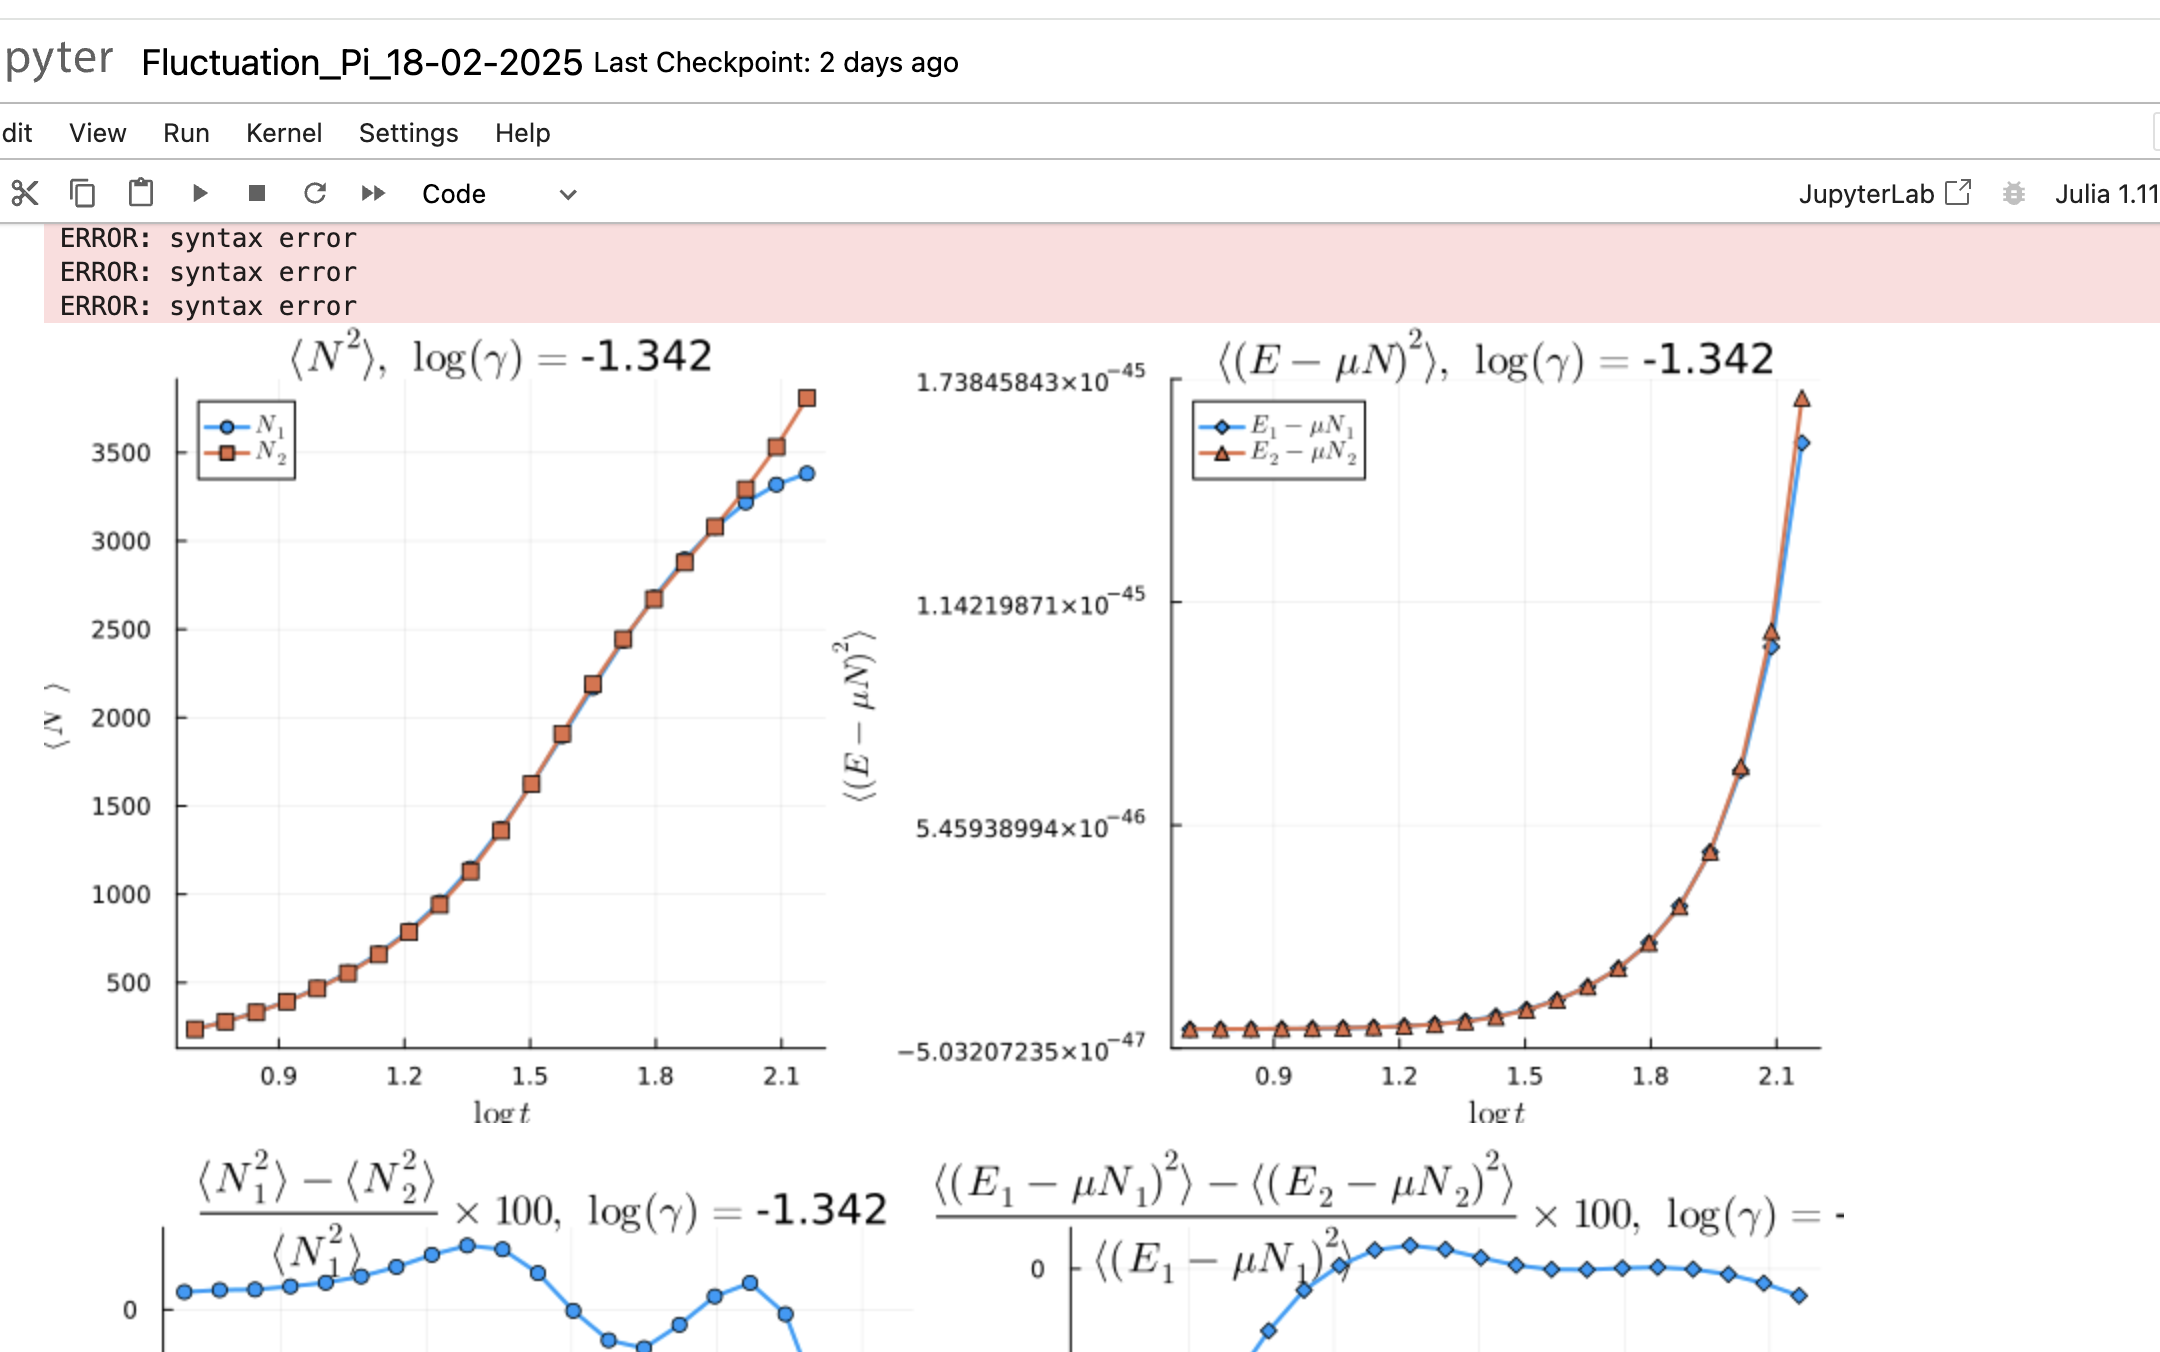
\includegraphics[width=1\textwidth]{Figures/test}

%\begin{aff}
%Donc une a l'ordre un en $\delta \theta (\operator{A}^{(0)})^{-1} %\operator{V}$ 

%\begin{eqnarray*}
%	\langle \delta \Pi ( \theta) \delta \Pi ( \theta') \rangle & = &  ( (\Pi^c_s - \Pi^c)\Pi^c/\Pi^c_s ) ( \theta ) \delta_{\theta, \theta'}/\delta \theta + \mathscr{F}(\theta , \theta' ) ,	
%\end{eqnarray*}

%avec 

%\begin{eqnarray*}
%	\mathscr{F}(\theta , \theta' ) & = & \left [ (\Pi^c_s - \Pi^c )( \theta)  +  (\Pi^c_s - \Pi^c ) ( \theta' )\right ] \frac{\Pi^c}{\Pi^c_s}(\theta)\frac{\Pi^c}{\Pi^c_s}(\theta') \frac{ \Delta( \theta'- \theta )}{ 2 \pi }\\
%	&&  - \left [ (\Pi^c_s - \Pi^c )( \theta)   (\Pi^c_s - \Pi^c ) ( \theta' )\right ] \frac{\Pi^c}{\Pi^c_s}(\theta)\frac{\Pi^c}{\Pi^c_s}(\theta')\int d\theta'' \left (   \frac{ \Pi^c/\Pi^c_s}{\Pi^c_s - \Pi^c} \right )(\theta'') \frac{\Delta(\theta''- \theta)}{2 \pi}\frac{\Delta(\theta''- \theta')}{2 \pi}  	
%\end{eqnarray*}
%\end{aff}



 











%\subsection{Introduction au modèle de gaz de Bose unidimensionnel et Hamiltonien du modèle}
%%Dans ce chapitre, nous nous intéressons aux fluctuations de la distribution de rapidité \( \delta \rho \) autour d'une distribution de référence \( \rho^c \), qui maximise la contribution à la fonction de partition des états, exprimée comme une fonctionnelle de la distribution \( \rho \) : 

La fonction de partition des états, s'exprime comme une fonctionnelle de la distribution \( \rho \) : 

\begin{eqnarray*}
	\Xi & = & \sum_\rho \exp \left( -\mathcal{A}(\rho) \right).
\end{eqnarray*}  

Dans la section {\em \bf Entropie de Yang-Yang} (\ref{??}), l'action \( \mathcal{A}(\rho) \) s'écrit sous la forme :  

\begin{eqnarray*}
	\mathcal{A}(\rho) & \doteq & - L\mathcal{S}_{YY}(\rho) + L\int f(\theta) \rho (\theta) \, d\theta,		
\end{eqnarray*}  

où \( \mathcal{S}_{YY} \) est la fonctionnelle d'entropie de Yang-Yang, définie dans (\ref{??}), et \( f \) est la fonction paramétrant les charges, introduite dans (\ref{??}).  

Dans cette même section {\em \bf Entropie de Yang-Yang} (\ref{??}), nous avons établi un lien entre \( f \) et distribution de référence \( \rho^c \), qui maximise la contribution à la fonction de partition des états .\\

On veux tester si nos experience est décrit pas un GGE. Pour cela nous nous intéressons aux fluctuations de la distribution de rapidité \( \delta \rho \) autour \( \rho^c \).

%Nous poursuivons à présent avec cette définition de l'action de classe $\mathcal{C}^2$ et admetant une distribution critique $\rho^c$ tel que sa différentielle en ce point critique soit nulle $d\mathcal{A}_{\rho^c} = 0 $ (\ref{??}) de sorte que d'aprés la formule de Taylor-Youg %afin de déterminer les fluctuations autour de \( \Pi^c \). Pour cela, nous réécrivons l'action sous la forme :  

Nous poursuivons à présent avec cette définition de l'action de classe $\mathcal{C}^2$ et admetant une distribution critique $\rho^c$ tel que sa différentielle en ce point critique soit nulle $d\mathcal{A}_{\rho^c} = 0 $ (\ref{??}) de sorte que d'aprés la formule de Taylor-Youg %afin de déterminer les fluctuations autour de \( \Pi^c \). Pour cela, nous réécrivons l'action sous la forme :  

\begin{eqnarray*}  
	\mathcal{A}(\rho^c + \delta \rho) & \underset{ \delta \rho \to 0 }{=} & \mathcal{A}(\rho^c)  + \frac{1}{2} \left. \frac{\delta^2 \mathcal{A}}{\delta \rho^2} \right|_{\rho^c} (\delta \rho) + \mathcal{O}((\delta \rho)^3),  
\end{eqnarray*}  

une expression quadratique pour l'action à l'ordre dominant en \( \delta \Pi \) avec $\left. \frac{\delta^2 \mathcal{A}}{\delta \rho^2} \right|_{\rho^c}$ la forme quadratique définie positive (Fig (\ref{fig.fluctu.A})).

\begin{figure}[H]
	\centering 
	\begin{tikzpicture}
		\begin{scope}[shift={(0,0)}]
			\begin{scope}[transform canvas={scale=0.6}]
				% Définition des couleurs avec les codes HTML
\definecolor{colorOne}{HTML}{443E46}
\definecolor{colorTwo}{HTML}{F6DEB8}
\definecolor{colorThree}{HTML}{908CA4}
\definecolor{colorFour}{HTML}{57659E}
\definecolor{colorFive}{HTML}{C57284}
\definecolor{colorSix}{HTML}{FF5B69}

% Raccourcis pour les couleurs
\def\colorOne{colorOne}
\def\colorTwo{colorTwo}
\def\colorThree{colorThree}
\def\colorFour{colorFour}
\def\colorFive{colorFive}
\def\colorSix{colorSix}

\def\colorslide{blue!50!black}



\begin{scope}
	% Tracer une courbe lisse entre des points
	\draw[shift={(0,0)} ,\colorOne]
		(-1 , 0 ) edge [thick,line width=0.8ex , ->,>=triangle 45  , \colorOne] node [pos = 1 , below ]{\huge$\rho$}( 5  , 0 )
	;
	\draw[shift={(0,0)}, color=\colorOne]
		(0, -1.0 ) edge [thick,line width=0.8ex , ->,>=triangle 45  ]node [pos=0.9,left=0.2cm ]{\huge$\mathcal{A}(\rho)$}( 0  , 5 )
	;
	\draw[]
		(2.5, 0.12 ) edge [thick,line width=0.8ex ,\colorThree ]node [pos=1,below  ]{\huge$\rho^c$} (2.5, -0.12 )	
	;
	
	\draw[]
		(2.5, -0.12 ) edge [thick,line width=0.4ex , dashed, \colorThree ] (2.5, 5.5 )
		(1.5, 1 ) edge [thick,line width=0.4ex , <->,>=triangle 45  , \colorThree ] (3.5, 1 )
		(-0.3,1) edge [thick,line width=0.4ex  , \colorThree ] node [pos=0,left ]{\huge$\mathcal{A}(\rho^c)$} (0.3, 1 )	
	;
    \draw[thick, line width=0.8ex , \colorFour] plot[smooth, tension=0.7] coordinates {
        (1, 5) (1.6 , 3 ) (2.5, 1) (3.5 , 3 )  (4, 5)
    };		
	
\end{scope}

	
			
			\end{scope}
			
			\draw[color = red , scale = 0.5 , draw = none  ] (-2 , -1) rectangle (5, 6) ; 	
		\end{scope}
		
		\begin{scope}[shift={(19,-1)}]
			\begin{scope}[transform canvas={scale=0.6}]
				% Définition des couleurs avec les codes HTML
\definecolor{colorOne}{HTML}{443E46}
\definecolor{colorTwo}{HTML}{F6DEB8}
\definecolor{colorThree}{HTML}{908CA4}
\definecolor{colorFour}{HTML}{57659E}
\definecolor{colorFive}{HTML}{C57284}
\definecolor{colorSix}{HTML}{FF5B69}

% Raccourcis pour les couleurs
\def\colorOne{colorOne}
\def\colorTwo{colorTwo}
\def\colorThree{colorThree}
\def\colorFour{colorFour}
\def\colorFive{colorFive}
\def\colorSix{colorSix}

\def\colorslide{blue!50!black}

\def\Occupation{
	\def\traitx{0.3}
	\def\traity{0.5}
	\draw[shift={(0,0)}]
		(-13.5 , 0 ) edge [thick,line width=0.8ex ]( -3.2  , 0 )
		( -3.2 - \traitx  , 0 - \traity ) edge [thick,line width=0.8ex ]( -3.2 + \traitx  , 0 + \traity  )
		( -2.8 - \traitx  , 0 - \traity ) edge [thick,line width=0.8ex ]( -2.8 + \traitx  , 0 + \traity  )
		(-2.8 , 0 ) edge [thick,line width=0.8ex ](2.8  , 0 )
		( 2.8 - \traitx  , 0 - \traity ) edge [thick,line width=0.8ex ]( 2.8 + \traitx  , 0 + \traity  )
		( 3.2 - \traitx  , 0 - \traity ) edge [thick,line width=0.8ex ]( 3.2 + \traitx  , 0 + \traity  )
		(3.2, 0 ) edge [thick,line width=0.8ex,->,>=triangle 45 , color = black ]node [pos=1.01,below  ]{\huge$\theta$}	( 13  , 0 )
	;
	\draw[shift={(0,0)}, color=\colorOne]
		(-10.5 , -1.5 ) edge [thick,line width=0.8ex , ->,>=triangle 45  ]( -10.5  , 4.5 )
	;
		
	\foreach \r in {1 , ... , 3 } {
%		\draw[
%		decoration={
%		markings,
%    	mark connection node=my node,
%    	mark=at position 0 with{\node [blue,transform shape] (my node) {\large \r};}},
%		color=gray, thick, 
%		line width=0.5ex] decorate { 
%            (-11.0, \r) -- (-10.1, \r )}
%        ;
        \draw[
			color=\colorOne,
			] 
            (-11.0, \r) edge[color=\colorThree , thick,line width=0.5ex] node [pos=-0.5 ]{\large\color{\colorFour} $\frac{\r}{\delta \theta}$ } (-10.3, \r )
        	;
	
	}
	

	
	% Graduation abcsisse 
	% Définitions des listes
% Definitions of the lists
\def\listetuple{-9/\theta_{1}, -8/\theta_{2} , -5/\theta_{3} , -2/\theta_{a-1} , 0/\theta_{a} , 1/\theta_{a+1} , 2/\theta_{a+2} ,  5/\theta_{N-4} , 7/\theta_{N-3},8/\theta_{N-1},9/\theta_{N} }
\def\listetrais{-12 , -11, -10, -9 , -8 , -7 ,  -6 , -5, -4.5,-4, -2 , -1, 0 , 0.5, 1, 2, 4 , 5 ,  6 , 7 , 8 ,8.5, 9 ,  10 , 11, 12 }

% Loop over listetrais
\foreach \r in \listetrais {
    % Initialize found variable to zero
    % Initialize found variable to zero
    %\pgfmathsetmacro\found{0}
    \global\def\found{0}
    \xdef\nomtheta{}
    
    % Check if \r is in listetuple
    \foreach \x/\y in \listetuple { 
        \ifdim \r pt=\x pt % If \r matches any \x in listetuple
            \global\def\found{1} ;
            \xdef\nomtheta{\y} % Set \nomtheta to the corresponding \y
            %\pgfmathsetmacro\found{1} % Set found to 1            
            %\global\pgfmathsetmacro\found{1}
        \fi
    }
    
    %\node [circle, draw, red] (A) at (\r, 2) {\found , $\nomtheta$};
    
    % Draw the line and display \nomtheta if found
    \ifnum\found=1
        \draw[color=\colorOne, thick, line width=0.5ex] 
            (\r, -0.3) -- (\r, 0.3) node[red , pos=-0.5] {\large $\nomtheta$};
         \filldraw[line width=0.5ex, color=\colorSix, outer color=\colorSix, inner color=\colorSix] 
            (\r, 0) circle (4pt);
    \else 
        % Draw without \nomtheta and add a blue circle if not found
        \draw[color=\colorOne, thick, line width=0.5ex] 
            (\r, -0.3) -- (\r, 0.3);
        \filldraw[line width=0.5ex, color=\colorSix, outer color=\colorTwo, inner color=\colorTwo] 
            (\r, 0) circle (4pt); 
    \fi
}

\def\listetrais{-9.5/\theta_{i-1}/2/3, -6.5/\theta_{i}/1/4  ,   -1.5/\theta_{j}/2/4 , 1.5/\theta_{j+1}/-1/3 , 3.5/\theta_{\ell-1}/1/3 , 6.5/\theta_{\ell}/3/4 , 9.5/\theta(\theta_{\ell+1})/-1/3 };



\foreach \r/\nomx/\y/\ys in \listetrais {
	\draw[
		decoration={
		markings,
    	mark connection node=my node,
    	mark=at position .5 with{\node [blue,transform shape] (my node) {\large \color{\colorFour} $\nomx$};}},
		color=\colorThree , thick, 
		line width=0.5ex] decorate { 
            (\r, 0.12) -- (\r, -1.2)}
        ;
     
     \ifdim \y pt > -1 pt 
     	\draw[
			decoration={
			markings,
    		mark connection node=my node,
    		mark=at position .5 with{\node [blue,transform shape] (my node) {\large \color{\colorFour} $\Pi(\nomx) $};}},
			color=\colorThree, thick, 
			line width=0.5ex] decorate { 
            (\r, \y) -- (\r +3, \y)}
        ;
        \draw[
			decoration={
			markings,
    		mark connection node=my node,
    		mark=at position .5 with{\node [blue,transform shape] (my node) {\large \color{\colorFive} $\Pi_s(\nomx) $};}},
			color=\colorFive, thick, 
			line width=0.5ex] decorate { 
            (\r, \ys) -- (\r +3, \ys)}
        ;
     \fi 
     \ifdim \r pt= -1.5 pt
     	\draw[
     		decoration={
			markings,
    		mark connection node=my node,
    		mark=at position .5 with{\node [blue,transform shape] (my node) {\large \color{\colorFour}  $\delta \theta $};},
    		%mark=at position 0.1  with {\arrow[blue, line width=0.5ex]{<}},
    		%mark=at position 1  with {\arrow[blue, line width=0.5ex]{>}}
    		},
        	color=\colorThree,
        	thick,
        	line width=0.5ex,
        	%arrows={Computer Modern Rightarrow[line cap=round]-Computer Modern Rightarrow[line cap=round]}
   			](\r, -1.2) edge[arrows={Computer Modern Rightarrow[line cap=round]-}] (\r + 0.4, -1.2)decorate {
    		(\r, -1.2) -- (\r + 3, -1.2)}(\r + 2, -1.2) edge[arrows={-Computer Modern Rightarrow[line cap=round]}] (\r + 3, -1.2)
    		;
    \fi
			
	
}


			
}


\begin{scope}
	%\draw[help lines , width=1.5ex] (-8,-3) grid (8,3);\draw[help lines ,width=0.5ex , opacity = 0.5] (-3,-3) grid[step=0.1] (3,3));
	
	%\draw[help lines] 
	%	(-3,-3) edge[width=1.5ex] grid (3,3)	
	%	(-3,-3) edge[width=0.5ex , opacity = 0.5] grid (3,3)	
	%;
	\begin{scope}[shift={(0,1)},rotate=0,opacity=1,color=black]
		\Occupation	
		
		%\node[anchor=east, font=\bfseries] at (-11, 0) {\color{red}\large (T = 0 )} ;	
	\end{scope}
	
	
	
	
	\begin{scope}[shift={(-10.5,7)},rotate=0,opacity=1,color=black]
	
	\begin{scope}[shift={(-0,0)},rotate=0,opacity=1,color=black]
	
		\draw[shift={(0,0)} ,line width=1ex,rounded corners = 1ex,color=\colorOne , opacity =1 ,fill=\colorOne!00 , pattern={north east lines} , pattern color=\colorOne!00 ]
			(0 , -1 ) rectangle (5,1)
		;
		

		\begin{scope}[shift={(0.5,0.5)}]
			\draw[color=\colorOne, thick, line width=0.5ex] 
            (0, -0.3) -- (0, 0.3) ;
            \filldraw[line width=0.5ex, color=\colorSix, outer color=\colorSix, inner color=\colorSix] 
            (0, 0) circle (4pt);
            
            \node[anchor=west, font=\bfseries] at (0.2, 0) {\color{\colorSix}\large : quasi-particule};
		\end{scope}
		
		\begin{scope}[shift={(0.5,-0.5)}]
			\draw[color=\colorOne, thick, line width=0.5ex] 
            (0, -0.3) -- (0, 0.3) ;
            \filldraw[line width=0.5ex, color=\colorSix, outer color=\colorTwo, inner color=\colorTwo] 
            (0, 0) circle (4pt);
            
            \node[anchor=west, font=\bfseries] at (0.2, 0) {\color{\colorSix}\large : hole};
		\end{scope}

	\end{scope}
	
	\begin{scope}[shift={(6,0)},rotate=0,opacity=1,color=black]	
		
		\draw[shift={(0,0)} ,line width=1ex,rounded corners = 1ex,color=\colorOne , opacity =1 ,fill=\colorOne!00 , pattern={north east lines} , pattern color=\colorOne!00 ]
			(0 , -1 ) rectangle (7.5,1)
		;
		
		\node[anchor=west] at (0.5, 0.5) {\color{\colorFour}\large $\Pi$ };\node[anchor=west, font=\bfseries] at (1, 0.5) {\color{\colorFour}\large : quasi-particule distribution};
		
		\node[anchor=west] at (0.5, -0.5) {\color{\colorFour}\large $\Pi_h$ };\node[anchor=west, font=\bfseries] at (1, -0.5) {\color{\colorFour}\large  : hole distribution};
		
	\end{scope}
	
	\begin{scope}[shift={(14.5,0)},rotate=0,opacity=1,color=black]	
		
		\draw[shift={(0,0)} ,line width=1ex,rounded corners = 1ex,color=\colorOne , opacity =1 ,fill=\colorOne!00 , pattern={north east lines} , pattern color=\colorOne!00 ]
			(0 , -0.5 ) rectangle (7.0,0.5)
		;
		
		\node[anchor=west] at (0.2, 0) {\color{\colorFour}\large ${\color{\colorFive}\Pi_s} = \Pi + \Pi_h $ } node[anchor=west , font=\bfseries] at (3.1 , 0 )  {\color{\colorFour}\large {\color{\colorFive} : density of states}};
		
	\end{scope}
	
	
	\end{scope}


		
	
\end{scope}

	
			
			\end{scope}
			\begin{scope}[scale=1]
				\draw[color = red , scale = 1 , draw = none  ] (-1 , -1) rectangle (5, 5) ; 
			\end{scope}	
		\end{scope}

		
				
			
	\end{tikzpicture}	
	\captionsetup{skip=10pt} % Ajoute de l’espace après la légende
	\label{fig.fluctu.A}
\end{figure}


On discrétise l'axe des rapidités en  petite cellule de rapidité $[\theta, \theta+\delta\theta]$, qui contient $L\rho(\theta) \delta \theta$ rapidités. 
	



Avec ces petites tranches, la forme quadratique s’écrit :

\begin{eqnarray*}
    \left. \frac{\delta^2 \mathcal{A}}{{\delta \rho}^2} \right|_{\rho^c}(\delta \rho ) &=&  \sum_{a,b \mid \text{tranche}}  
    \delta \rho(\theta_a)  \frac{\partial^2 \mathcal{A}}{\partial \delta \rho(\theta_a) \partial \delta \rho(\theta_b) } (\rho^c)  \delta \rho(\theta_b).
\end{eqnarray*}
Les fluctuations s’écrivent donc :

\begin{eqnarray*}
    \langle \delta \rho ( \theta) \delta \rho ( \theta') \rangle &=&  
    \frac{ \int d\delta \rho \, \delta \rho(\theta) \delta \rho ( \theta') 
    \exp \left( - \frac{1}{2} \sum_{a,b \mid \text{tranche}}  
    \delta \rho(\theta_a) \frac{\partial^2 \mathcal{A}}{\partial \delta \rho(\theta_a) \partial \delta \rho(\theta_b) } (\rho^c)  \delta \rho(\theta_b) \right) }
    { \int d\delta \Pi  
    \exp \left( - \frac{1}{2} \sum_{a,b \mid \text{tranche}}  
    \delta \rho(\theta_a) \frac{\partial^2 \mathcal{A}}{\partial \delta \rho(\theta_a) \partial \delta \rho(\theta_b) } (\rho^c)  \delta \rho(\theta_b) \right) } \\
    &=& \left( \mathbf{A}^{-1} \right)_{\theta , \theta'}
\end{eqnarray*}


\begin{aff}

\begin{eqnarray*}
	\langle \delta \rho ( \theta) \delta \rho ( \theta') \rangle &=& 	\left( \mathbf{A}^{-1} \right)_{\theta , \theta'}
\end{eqnarray*}

	
avec la  {\em matrice hessienne} $\mathbf{A}_{\theta , \theta'} \equiv \frac{\partial^2 \mathcal{A}}{\partial \delta \rho(\theta) \partial \delta \rho(\theta') }(\rho^c)$, au point critique/ qui maximise la probabilité  $\rho^c=\rho^c_s \nu^c $, s'écrit

\begin{eqnarray*}
	\operator{A} & = & \operator{A}^{(0)} + \delta \theta \operator{V}
\end{eqnarray*}

avec 

\begin{eqnarray*}
	A^{(0)}_{\theta , \theta'}  & = &  L\delta \theta \left ( \frac{ 1}{\rho^c_s ( 1  - \nu^c ) \nu^c } \right )(\theta)    \delta({\theta - \theta '})	,\\
	V_{\theta , \theta'}  &= & L \delta \theta \left \{ - \left [ \left ( \frac{1}{\rho^c_s( 1 - \nu^c) } \right ) ( \theta)  +  \left ( \frac{1}{\rho^c_s( 1 - \nu^c) } \right ) ( \theta' )\right ] \frac{ \Delta( \theta'- \theta )}{ 2 \pi } + \int d\theta''  \left ( \frac{\nu^c}{\rho^c_s( 1 - \nu^c) } \right )(\theta'') \frac{\Delta(\theta''- \theta)}{2 \pi}\frac{\Delta(\theta''- \theta')}{2 \pi}   \right \} 	
\end{eqnarray*}

\end{aff}

\subsection{Testes}

\begin{eqnarray*}
	\Delta_{\operator{\mathcal{N}}}^2  & = &  \frac{1}{\beta} \left . \frac{\partial \langle \operator{\mathcal{N}} \rangle}{\partial \mu} \right )_T \\
	\Delta_{\operator{\mathcal{E}}-\mu \operator{\mathcal{N}}}^2  & = &  - \left . \frac{\partial \langle \operator{\mathcal{E}}-\mu \operator{\mathcal{N}} \rangle}{\partial \beta} \right )_\mu 
\end{eqnarray*}

et 

\begin{eqnarray*}
	\Delta_{\operator{\mathcal{N}}}^2  &= & L^2 \int d\theta_a \int d \theta_b \, \langle \delta \rho(\theta_a) \delta \rho(\theta_b) \rangle \\
	\Delta_{\operator{\mathcal{E}}-\mu \operator{\mathcal{N}}}^2  & = & L^2 \int d\theta_a \int d \theta_b \, \left ( - \mu + \frac{1}2 m \theta_a^2  \right  )\left ( - \mu + \frac{1}2 m \theta_b^2  \right  )  \langle \delta \rho(\theta_a) \delta \rho(\theta_b) \rangle
\end{eqnarray*}

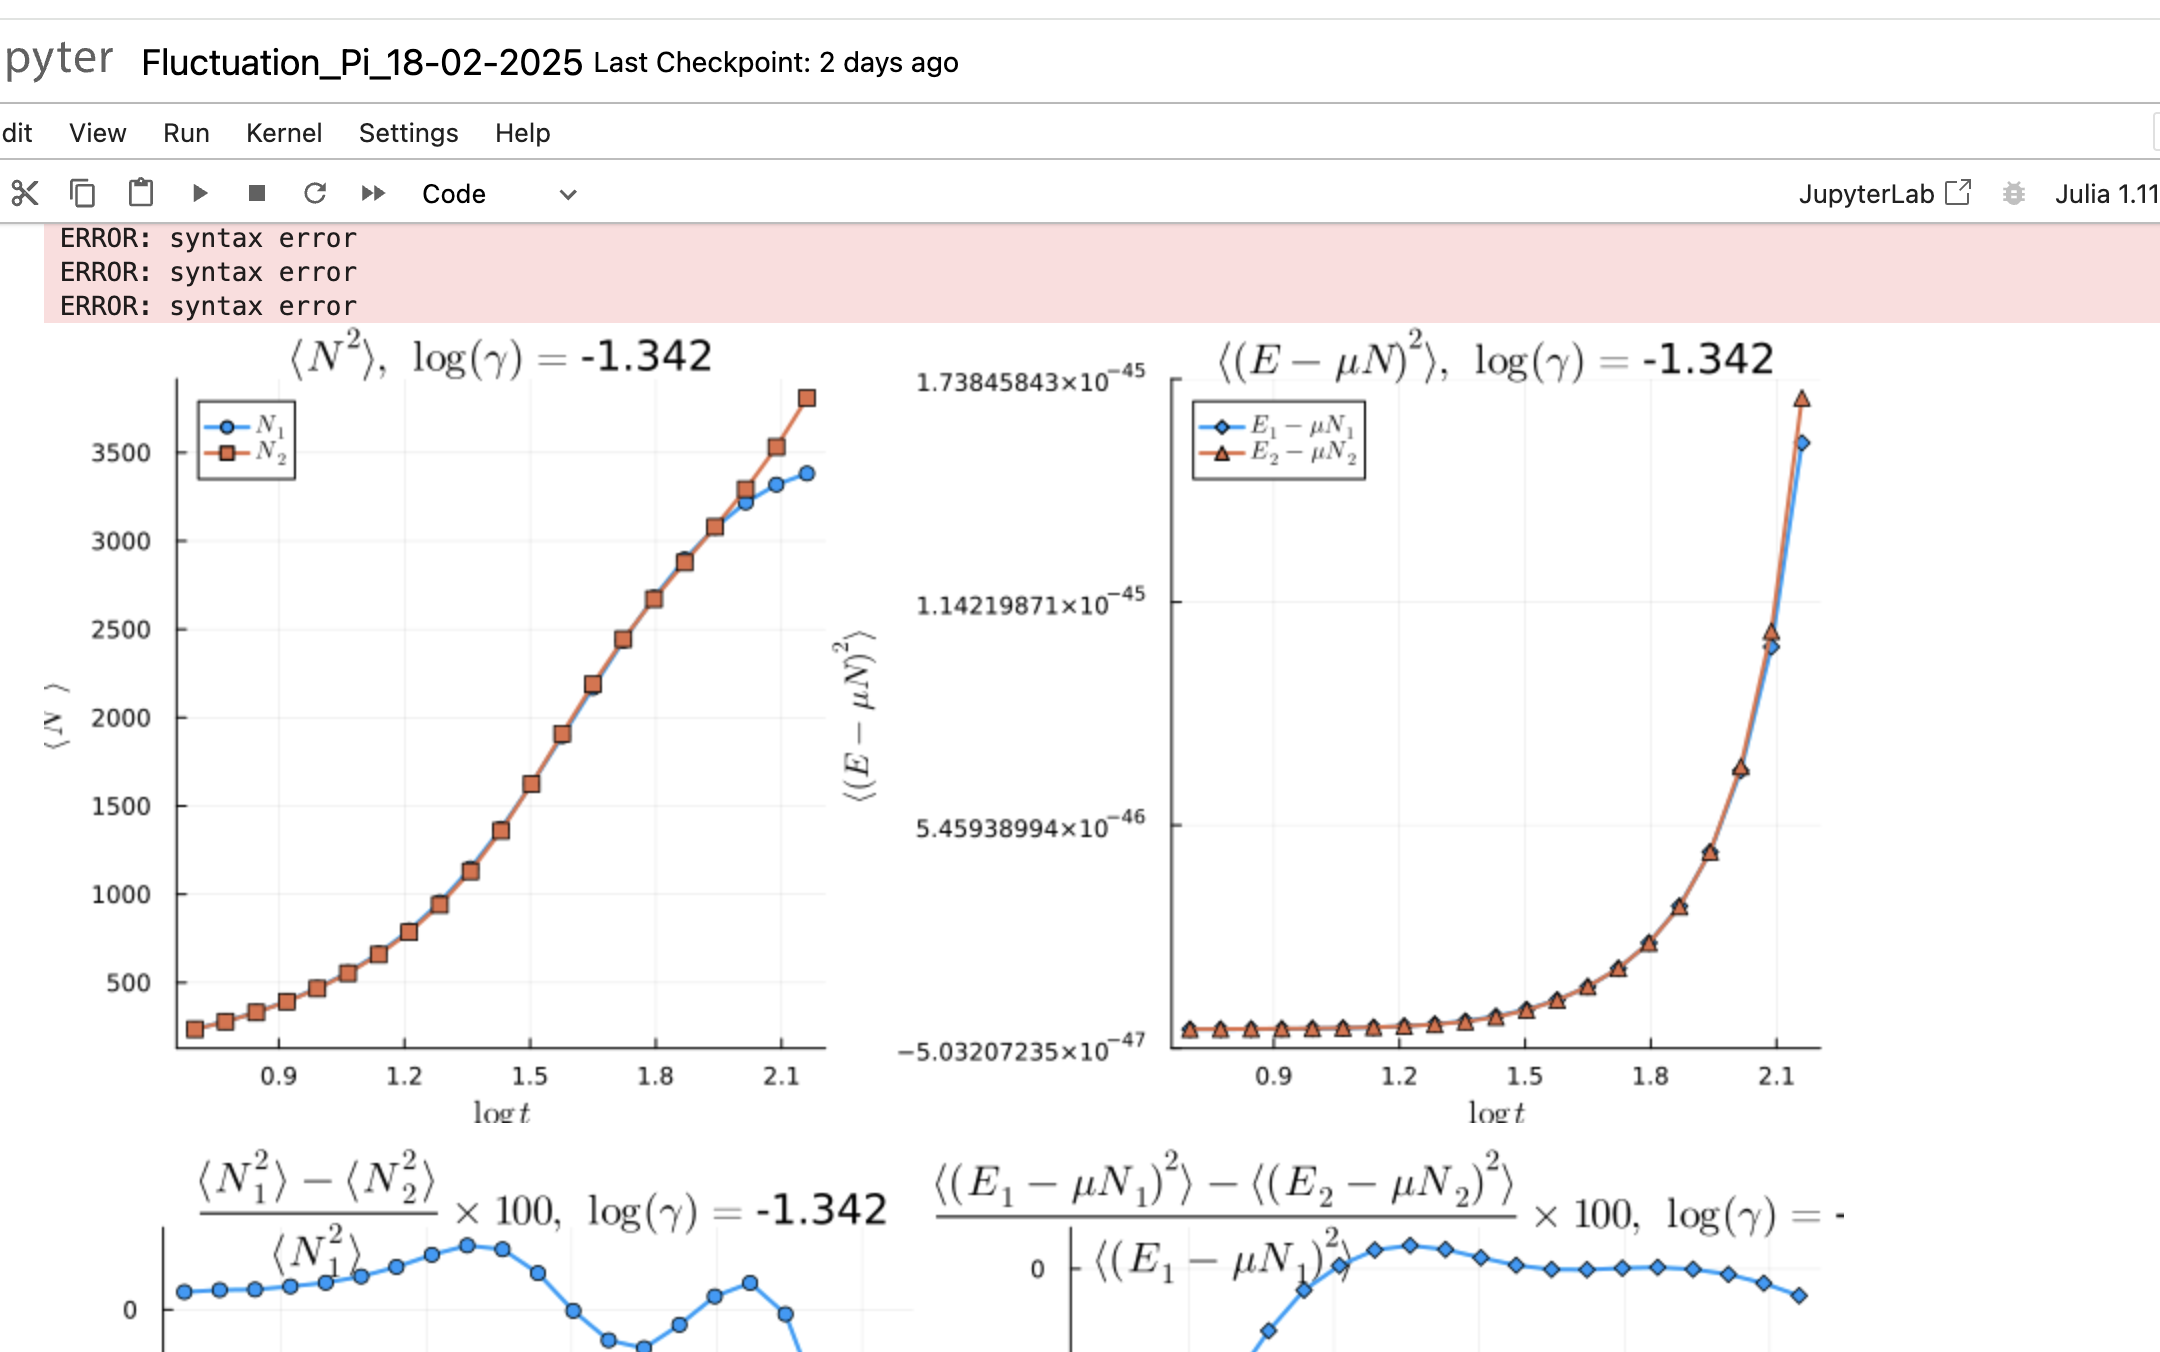
\includegraphics[width=1\textwidth]{Figures/test}

%\begin{aff}
%Donc une a l'ordre un en $\delta \theta (\operator{A}^{(0)})^{-1} %\operator{V}$ 

%\begin{eqnarray*}
%	\langle \delta \Pi ( \theta) \delta \Pi ( \theta') \rangle & = &  ( (\Pi^c_s - \Pi^c)\Pi^c/\Pi^c_s ) ( \theta ) \delta_{\theta, \theta'}/\delta \theta + \mathscr{F}(\theta , \theta' ) ,	
%\end{eqnarray*}

%avec 

%\begin{eqnarray*}
%	\mathscr{F}(\theta , \theta' ) & = & \left [ (\Pi^c_s - \Pi^c )( \theta)  +  (\Pi^c_s - \Pi^c ) ( \theta' )\right ] \frac{\Pi^c}{\Pi^c_s}(\theta)\frac{\Pi^c}{\Pi^c_s}(\theta') \frac{ \Delta( \theta'- \theta )}{ 2 \pi }\\
%	&&  - \left [ (\Pi^c_s - \Pi^c )( \theta)   (\Pi^c_s - \Pi^c ) ( \theta' )\right ] \frac{\Pi^c}{\Pi^c_s}(\theta)\frac{\Pi^c}{\Pi^c_s}(\theta')\int d\theta'' \left (   \frac{ \Pi^c/\Pi^c_s}{\Pi^c_s - \Pi^c} \right )(\theta'') \frac{\Delta(\theta''- \theta)}{2 \pi}\frac{\Delta(\theta''- \theta')}{2 \pi}  	
%\end{eqnarray*}
%\end{aff}



 








%\subsection{Hamiltonien du modèle}
%%Dans ce chapitre, nous nous intéressons aux fluctuations de la distribution de rapidité \( \delta \rho \) autour d'une distribution de référence \( \rho^c \), qui maximise la contribution à la fonction de partition des états, exprimée comme une fonctionnelle de la distribution \( \rho \) : 

La fonction de partition des états, s'exprime comme une fonctionnelle de la distribution \( \rho \) : 

\begin{eqnarray*}
	\Xi & = & \sum_\rho \exp \left( -\mathcal{A}(\rho) \right).
\end{eqnarray*}  

Dans la section {\em \bf Entropie de Yang-Yang} (\ref{??}), l'action \( \mathcal{A}(\rho) \) s'écrit sous la forme :  

\begin{eqnarray*}
	\mathcal{A}(\rho) & \doteq & - L\mathcal{S}_{YY}(\rho) + L\int f(\theta) \rho (\theta) \, d\theta,		
\end{eqnarray*}  

où \( \mathcal{S}_{YY} \) est la fonctionnelle d'entropie de Yang-Yang, définie dans (\ref{??}), et \( f \) est la fonction paramétrant les charges, introduite dans (\ref{??}).  

Dans cette même section {\em \bf Entropie de Yang-Yang} (\ref{??}), nous avons établi un lien entre \( f \) et distribution de référence \( \rho^c \), qui maximise la contribution à la fonction de partition des états .\\

On veux tester si nos experience est décrit pas un GGE. Pour cela nous nous intéressons aux fluctuations de la distribution de rapidité \( \delta \rho \) autour \( \rho^c \).

%Nous poursuivons à présent avec cette définition de l'action de classe $\mathcal{C}^2$ et admetant une distribution critique $\rho^c$ tel que sa différentielle en ce point critique soit nulle $d\mathcal{A}_{\rho^c} = 0 $ (\ref{??}) de sorte que d'aprés la formule de Taylor-Youg %afin de déterminer les fluctuations autour de \( \Pi^c \). Pour cela, nous réécrivons l'action sous la forme :  

Nous poursuivons à présent avec cette définition de l'action de classe $\mathcal{C}^2$ et admetant une distribution critique $\rho^c$ tel que sa différentielle en ce point critique soit nulle $d\mathcal{A}_{\rho^c} = 0 $ (\ref{??}) de sorte que d'aprés la formule de Taylor-Youg %afin de déterminer les fluctuations autour de \( \Pi^c \). Pour cela, nous réécrivons l'action sous la forme :  

\begin{eqnarray*}  
	\mathcal{A}(\rho^c + \delta \rho) & \underset{ \delta \rho \to 0 }{=} & \mathcal{A}(\rho^c)  + \frac{1}{2} \left. \frac{\delta^2 \mathcal{A}}{\delta \rho^2} \right|_{\rho^c} (\delta \rho) + \mathcal{O}((\delta \rho)^3),  
\end{eqnarray*}  

une expression quadratique pour l'action à l'ordre dominant en \( \delta \Pi \) avec $\left. \frac{\delta^2 \mathcal{A}}{\delta \rho^2} \right|_{\rho^c}$ la forme quadratique définie positive (Fig (\ref{fig.fluctu.A})).

\begin{figure}[H]
	\centering 
	\begin{tikzpicture}
		\begin{scope}[shift={(0,0)}]
			\begin{scope}[transform canvas={scale=0.6}]
				% Définition des couleurs avec les codes HTML
\definecolor{colorOne}{HTML}{443E46}
\definecolor{colorTwo}{HTML}{F6DEB8}
\definecolor{colorThree}{HTML}{908CA4}
\definecolor{colorFour}{HTML}{57659E}
\definecolor{colorFive}{HTML}{C57284}
\definecolor{colorSix}{HTML}{FF5B69}

% Raccourcis pour les couleurs
\def\colorOne{colorOne}
\def\colorTwo{colorTwo}
\def\colorThree{colorThree}
\def\colorFour{colorFour}
\def\colorFive{colorFive}
\def\colorSix{colorSix}

\def\colorslide{blue!50!black}



\begin{scope}
	% Tracer une courbe lisse entre des points
	\draw[shift={(0,0)} ,\colorOne]
		(-1 , 0 ) edge [thick,line width=0.8ex , ->,>=triangle 45  , \colorOne] node [pos = 1 , below ]{\huge$\rho$}( 5  , 0 )
	;
	\draw[shift={(0,0)}, color=\colorOne]
		(0, -1.0 ) edge [thick,line width=0.8ex , ->,>=triangle 45  ]node [pos=0.9,left=0.2cm ]{\huge$\mathcal{A}(\rho)$}( 0  , 5 )
	;
	\draw[]
		(2.5, 0.12 ) edge [thick,line width=0.8ex ,\colorThree ]node [pos=1,below  ]{\huge$\rho^c$} (2.5, -0.12 )	
	;
	
	\draw[]
		(2.5, -0.12 ) edge [thick,line width=0.4ex , dashed, \colorThree ] (2.5, 5.5 )
		(1.5, 1 ) edge [thick,line width=0.4ex , <->,>=triangle 45  , \colorThree ] (3.5, 1 )
		(-0.3,1) edge [thick,line width=0.4ex  , \colorThree ] node [pos=0,left ]{\huge$\mathcal{A}(\rho^c)$} (0.3, 1 )	
	;
    \draw[thick, line width=0.8ex , \colorFour] plot[smooth, tension=0.7] coordinates {
        (1, 5) (1.6 , 3 ) (2.5, 1) (3.5 , 3 )  (4, 5)
    };		
	
\end{scope}

	
			
			\end{scope}
			
			\draw[color = red , scale = 0.5 , draw = none  ] (-2 , -1) rectangle (5, 6) ; 	
		\end{scope}
		
		\begin{scope}[shift={(19,-1)}]
			\begin{scope}[transform canvas={scale=0.6}]
				% Définition des couleurs avec les codes HTML
\definecolor{colorOne}{HTML}{443E46}
\definecolor{colorTwo}{HTML}{F6DEB8}
\definecolor{colorThree}{HTML}{908CA4}
\definecolor{colorFour}{HTML}{57659E}
\definecolor{colorFive}{HTML}{C57284}
\definecolor{colorSix}{HTML}{FF5B69}

% Raccourcis pour les couleurs
\def\colorOne{colorOne}
\def\colorTwo{colorTwo}
\def\colorThree{colorThree}
\def\colorFour{colorFour}
\def\colorFive{colorFive}
\def\colorSix{colorSix}

\def\colorslide{blue!50!black}

\def\Occupation{
	\def\traitx{0.3}
	\def\traity{0.5}
	\draw[shift={(0,0)}]
		(-13.5 , 0 ) edge [thick,line width=0.8ex ]( -3.2  , 0 )
		( -3.2 - \traitx  , 0 - \traity ) edge [thick,line width=0.8ex ]( -3.2 + \traitx  , 0 + \traity  )
		( -2.8 - \traitx  , 0 - \traity ) edge [thick,line width=0.8ex ]( -2.8 + \traitx  , 0 + \traity  )
		(-2.8 , 0 ) edge [thick,line width=0.8ex ](2.8  , 0 )
		( 2.8 - \traitx  , 0 - \traity ) edge [thick,line width=0.8ex ]( 2.8 + \traitx  , 0 + \traity  )
		( 3.2 - \traitx  , 0 - \traity ) edge [thick,line width=0.8ex ]( 3.2 + \traitx  , 0 + \traity  )
		(3.2, 0 ) edge [thick,line width=0.8ex,->,>=triangle 45 , color = black ]node [pos=1.01,below  ]{\huge$\theta$}	( 13  , 0 )
	;
	\draw[shift={(0,0)}, color=\colorOne]
		(-10.5 , -1.5 ) edge [thick,line width=0.8ex , ->,>=triangle 45  ]( -10.5  , 4.5 )
	;
		
	\foreach \r in {1 , ... , 3 } {
%		\draw[
%		decoration={
%		markings,
%    	mark connection node=my node,
%    	mark=at position 0 with{\node [blue,transform shape] (my node) {\large \r};}},
%		color=gray, thick, 
%		line width=0.5ex] decorate { 
%            (-11.0, \r) -- (-10.1, \r )}
%        ;
        \draw[
			color=\colorOne,
			] 
            (-11.0, \r) edge[color=\colorThree , thick,line width=0.5ex] node [pos=-0.5 ]{\large\color{\colorFour} $\frac{\r}{\delta \theta}$ } (-10.3, \r )
        	;
	
	}
	

	
	% Graduation abcsisse 
	% Définitions des listes
% Definitions of the lists
\def\listetuple{-9/\theta_{1}, -8/\theta_{2} , -5/\theta_{3} , -2/\theta_{a-1} , 0/\theta_{a} , 1/\theta_{a+1} , 2/\theta_{a+2} ,  5/\theta_{N-4} , 7/\theta_{N-3},8/\theta_{N-1},9/\theta_{N} }
\def\listetrais{-12 , -11, -10, -9 , -8 , -7 ,  -6 , -5, -4.5,-4, -2 , -1, 0 , 0.5, 1, 2, 4 , 5 ,  6 , 7 , 8 ,8.5, 9 ,  10 , 11, 12 }

% Loop over listetrais
\foreach \r in \listetrais {
    % Initialize found variable to zero
    % Initialize found variable to zero
    %\pgfmathsetmacro\found{0}
    \global\def\found{0}
    \xdef\nomtheta{}
    
    % Check if \r is in listetuple
    \foreach \x/\y in \listetuple { 
        \ifdim \r pt=\x pt % If \r matches any \x in listetuple
            \global\def\found{1} ;
            \xdef\nomtheta{\y} % Set \nomtheta to the corresponding \y
            %\pgfmathsetmacro\found{1} % Set found to 1            
            %\global\pgfmathsetmacro\found{1}
        \fi
    }
    
    %\node [circle, draw, red] (A) at (\r, 2) {\found , $\nomtheta$};
    
    % Draw the line and display \nomtheta if found
    \ifnum\found=1
        \draw[color=\colorOne, thick, line width=0.5ex] 
            (\r, -0.3) -- (\r, 0.3) node[red , pos=-0.5] {\large $\nomtheta$};
         \filldraw[line width=0.5ex, color=\colorSix, outer color=\colorSix, inner color=\colorSix] 
            (\r, 0) circle (4pt);
    \else 
        % Draw without \nomtheta and add a blue circle if not found
        \draw[color=\colorOne, thick, line width=0.5ex] 
            (\r, -0.3) -- (\r, 0.3);
        \filldraw[line width=0.5ex, color=\colorSix, outer color=\colorTwo, inner color=\colorTwo] 
            (\r, 0) circle (4pt); 
    \fi
}

\def\listetrais{-9.5/\theta_{i-1}/2/3, -6.5/\theta_{i}/1/4  ,   -1.5/\theta_{j}/2/4 , 1.5/\theta_{j+1}/-1/3 , 3.5/\theta_{\ell-1}/1/3 , 6.5/\theta_{\ell}/3/4 , 9.5/\theta(\theta_{\ell+1})/-1/3 };



\foreach \r/\nomx/\y/\ys in \listetrais {
	\draw[
		decoration={
		markings,
    	mark connection node=my node,
    	mark=at position .5 with{\node [blue,transform shape] (my node) {\large \color{\colorFour} $\nomx$};}},
		color=\colorThree , thick, 
		line width=0.5ex] decorate { 
            (\r, 0.12) -- (\r, -1.2)}
        ;
     
     \ifdim \y pt > -1 pt 
     	\draw[
			decoration={
			markings,
    		mark connection node=my node,
    		mark=at position .5 with{\node [blue,transform shape] (my node) {\large \color{\colorFour} $\Pi(\nomx) $};}},
			color=\colorThree, thick, 
			line width=0.5ex] decorate { 
            (\r, \y) -- (\r +3, \y)}
        ;
        \draw[
			decoration={
			markings,
    		mark connection node=my node,
    		mark=at position .5 with{\node [blue,transform shape] (my node) {\large \color{\colorFive} $\Pi_s(\nomx) $};}},
			color=\colorFive, thick, 
			line width=0.5ex] decorate { 
            (\r, \ys) -- (\r +3, \ys)}
        ;
     \fi 
     \ifdim \r pt= -1.5 pt
     	\draw[
     		decoration={
			markings,
    		mark connection node=my node,
    		mark=at position .5 with{\node [blue,transform shape] (my node) {\large \color{\colorFour}  $\delta \theta $};},
    		%mark=at position 0.1  with {\arrow[blue, line width=0.5ex]{<}},
    		%mark=at position 1  with {\arrow[blue, line width=0.5ex]{>}}
    		},
        	color=\colorThree,
        	thick,
        	line width=0.5ex,
        	%arrows={Computer Modern Rightarrow[line cap=round]-Computer Modern Rightarrow[line cap=round]}
   			](\r, -1.2) edge[arrows={Computer Modern Rightarrow[line cap=round]-}] (\r + 0.4, -1.2)decorate {
    		(\r, -1.2) -- (\r + 3, -1.2)}(\r + 2, -1.2) edge[arrows={-Computer Modern Rightarrow[line cap=round]}] (\r + 3, -1.2)
    		;
    \fi
			
	
}


			
}


\begin{scope}
	%\draw[help lines , width=1.5ex] (-8,-3) grid (8,3);\draw[help lines ,width=0.5ex , opacity = 0.5] (-3,-3) grid[step=0.1] (3,3));
	
	%\draw[help lines] 
	%	(-3,-3) edge[width=1.5ex] grid (3,3)	
	%	(-3,-3) edge[width=0.5ex , opacity = 0.5] grid (3,3)	
	%;
	\begin{scope}[shift={(0,1)},rotate=0,opacity=1,color=black]
		\Occupation	
		
		%\node[anchor=east, font=\bfseries] at (-11, 0) {\color{red}\large (T = 0 )} ;	
	\end{scope}
	
	
	
	
	\begin{scope}[shift={(-10.5,7)},rotate=0,opacity=1,color=black]
	
	\begin{scope}[shift={(-0,0)},rotate=0,opacity=1,color=black]
	
		\draw[shift={(0,0)} ,line width=1ex,rounded corners = 1ex,color=\colorOne , opacity =1 ,fill=\colorOne!00 , pattern={north east lines} , pattern color=\colorOne!00 ]
			(0 , -1 ) rectangle (5,1)
		;
		

		\begin{scope}[shift={(0.5,0.5)}]
			\draw[color=\colorOne, thick, line width=0.5ex] 
            (0, -0.3) -- (0, 0.3) ;
            \filldraw[line width=0.5ex, color=\colorSix, outer color=\colorSix, inner color=\colorSix] 
            (0, 0) circle (4pt);
            
            \node[anchor=west, font=\bfseries] at (0.2, 0) {\color{\colorSix}\large : quasi-particule};
		\end{scope}
		
		\begin{scope}[shift={(0.5,-0.5)}]
			\draw[color=\colorOne, thick, line width=0.5ex] 
            (0, -0.3) -- (0, 0.3) ;
            \filldraw[line width=0.5ex, color=\colorSix, outer color=\colorTwo, inner color=\colorTwo] 
            (0, 0) circle (4pt);
            
            \node[anchor=west, font=\bfseries] at (0.2, 0) {\color{\colorSix}\large : hole};
		\end{scope}

	\end{scope}
	
	\begin{scope}[shift={(6,0)},rotate=0,opacity=1,color=black]	
		
		\draw[shift={(0,0)} ,line width=1ex,rounded corners = 1ex,color=\colorOne , opacity =1 ,fill=\colorOne!00 , pattern={north east lines} , pattern color=\colorOne!00 ]
			(0 , -1 ) rectangle (7.5,1)
		;
		
		\node[anchor=west] at (0.5, 0.5) {\color{\colorFour}\large $\Pi$ };\node[anchor=west, font=\bfseries] at (1, 0.5) {\color{\colorFour}\large : quasi-particule distribution};
		
		\node[anchor=west] at (0.5, -0.5) {\color{\colorFour}\large $\Pi_h$ };\node[anchor=west, font=\bfseries] at (1, -0.5) {\color{\colorFour}\large  : hole distribution};
		
	\end{scope}
	
	\begin{scope}[shift={(14.5,0)},rotate=0,opacity=1,color=black]	
		
		\draw[shift={(0,0)} ,line width=1ex,rounded corners = 1ex,color=\colorOne , opacity =1 ,fill=\colorOne!00 , pattern={north east lines} , pattern color=\colorOne!00 ]
			(0 , -0.5 ) rectangle (7.0,0.5)
		;
		
		\node[anchor=west] at (0.2, 0) {\color{\colorFour}\large ${\color{\colorFive}\Pi_s} = \Pi + \Pi_h $ } node[anchor=west , font=\bfseries] at (3.1 , 0 )  {\color{\colorFour}\large {\color{\colorFive} : density of states}};
		
	\end{scope}
	
	
	\end{scope}


		
	
\end{scope}

	
			
			\end{scope}
			\begin{scope}[scale=1]
				\draw[color = red , scale = 1 , draw = none  ] (-1 , -1) rectangle (5, 5) ; 
			\end{scope}	
		\end{scope}

		
				
			
	\end{tikzpicture}	
	\captionsetup{skip=10pt} % Ajoute de l’espace après la légende
	\label{fig.fluctu.A}
\end{figure}


On discrétise l'axe des rapidités en  petite cellule de rapidité $[\theta, \theta+\delta\theta]$, qui contient $L\rho(\theta) \delta \theta$ rapidités. 
	



Avec ces petites tranches, la forme quadratique s’écrit :

\begin{eqnarray*}
    \left. \frac{\delta^2 \mathcal{A}}{{\delta \rho}^2} \right|_{\rho^c}(\delta \rho ) &=&  \sum_{a,b \mid \text{tranche}}  
    \delta \rho(\theta_a)  \frac{\partial^2 \mathcal{A}}{\partial \delta \rho(\theta_a) \partial \delta \rho(\theta_b) } (\rho^c)  \delta \rho(\theta_b).
\end{eqnarray*}
Les fluctuations s’écrivent donc :

\begin{eqnarray*}
    \langle \delta \rho ( \theta) \delta \rho ( \theta') \rangle &=&  
    \frac{ \int d\delta \rho \, \delta \rho(\theta) \delta \rho ( \theta') 
    \exp \left( - \frac{1}{2} \sum_{a,b \mid \text{tranche}}  
    \delta \rho(\theta_a) \frac{\partial^2 \mathcal{A}}{\partial \delta \rho(\theta_a) \partial \delta \rho(\theta_b) } (\rho^c)  \delta \rho(\theta_b) \right) }
    { \int d\delta \Pi  
    \exp \left( - \frac{1}{2} \sum_{a,b \mid \text{tranche}}  
    \delta \rho(\theta_a) \frac{\partial^2 \mathcal{A}}{\partial \delta \rho(\theta_a) \partial \delta \rho(\theta_b) } (\rho^c)  \delta \rho(\theta_b) \right) } \\
    &=& \left( \mathbf{A}^{-1} \right)_{\theta , \theta'}
\end{eqnarray*}


\begin{aff}

\begin{eqnarray*}
	\langle \delta \rho ( \theta) \delta \rho ( \theta') \rangle &=& 	\left( \mathbf{A}^{-1} \right)_{\theta , \theta'}
\end{eqnarray*}

	
avec la  {\em matrice hessienne} $\mathbf{A}_{\theta , \theta'} \equiv \frac{\partial^2 \mathcal{A}}{\partial \delta \rho(\theta) \partial \delta \rho(\theta') }(\rho^c)$, au point critique/ qui maximise la probabilité  $\rho^c=\rho^c_s \nu^c $, s'écrit

\begin{eqnarray*}
	\operator{A} & = & \operator{A}^{(0)} + \delta \theta \operator{V}
\end{eqnarray*}

avec 

\begin{eqnarray*}
	A^{(0)}_{\theta , \theta'}  & = &  L\delta \theta \left ( \frac{ 1}{\rho^c_s ( 1  - \nu^c ) \nu^c } \right )(\theta)    \delta({\theta - \theta '})	,\\
	V_{\theta , \theta'}  &= & L \delta \theta \left \{ - \left [ \left ( \frac{1}{\rho^c_s( 1 - \nu^c) } \right ) ( \theta)  +  \left ( \frac{1}{\rho^c_s( 1 - \nu^c) } \right ) ( \theta' )\right ] \frac{ \Delta( \theta'- \theta )}{ 2 \pi } + \int d\theta''  \left ( \frac{\nu^c}{\rho^c_s( 1 - \nu^c) } \right )(\theta'') \frac{\Delta(\theta''- \theta)}{2 \pi}\frac{\Delta(\theta''- \theta')}{2 \pi}   \right \} 	
\end{eqnarray*}

\end{aff}

\subsection{Testes}

\begin{eqnarray*}
	\Delta_{\operator{\mathcal{N}}}^2  & = &  \frac{1}{\beta} \left . \frac{\partial \langle \operator{\mathcal{N}} \rangle}{\partial \mu} \right )_T \\
	\Delta_{\operator{\mathcal{E}}-\mu \operator{\mathcal{N}}}^2  & = &  - \left . \frac{\partial \langle \operator{\mathcal{E}}-\mu \operator{\mathcal{N}} \rangle}{\partial \beta} \right )_\mu 
\end{eqnarray*}

et 

\begin{eqnarray*}
	\Delta_{\operator{\mathcal{N}}}^2  &= & L^2 \int d\theta_a \int d \theta_b \, \langle \delta \rho(\theta_a) \delta \rho(\theta_b) \rangle \\
	\Delta_{\operator{\mathcal{E}}-\mu \operator{\mathcal{N}}}^2  & = & L^2 \int d\theta_a \int d \theta_b \, \left ( - \mu + \frac{1}2 m \theta_a^2  \right  )\left ( - \mu + \frac{1}2 m \theta_b^2  \right  )  \langle \delta \rho(\theta_a) \delta \rho(\theta_b) \rangle
\end{eqnarray*}

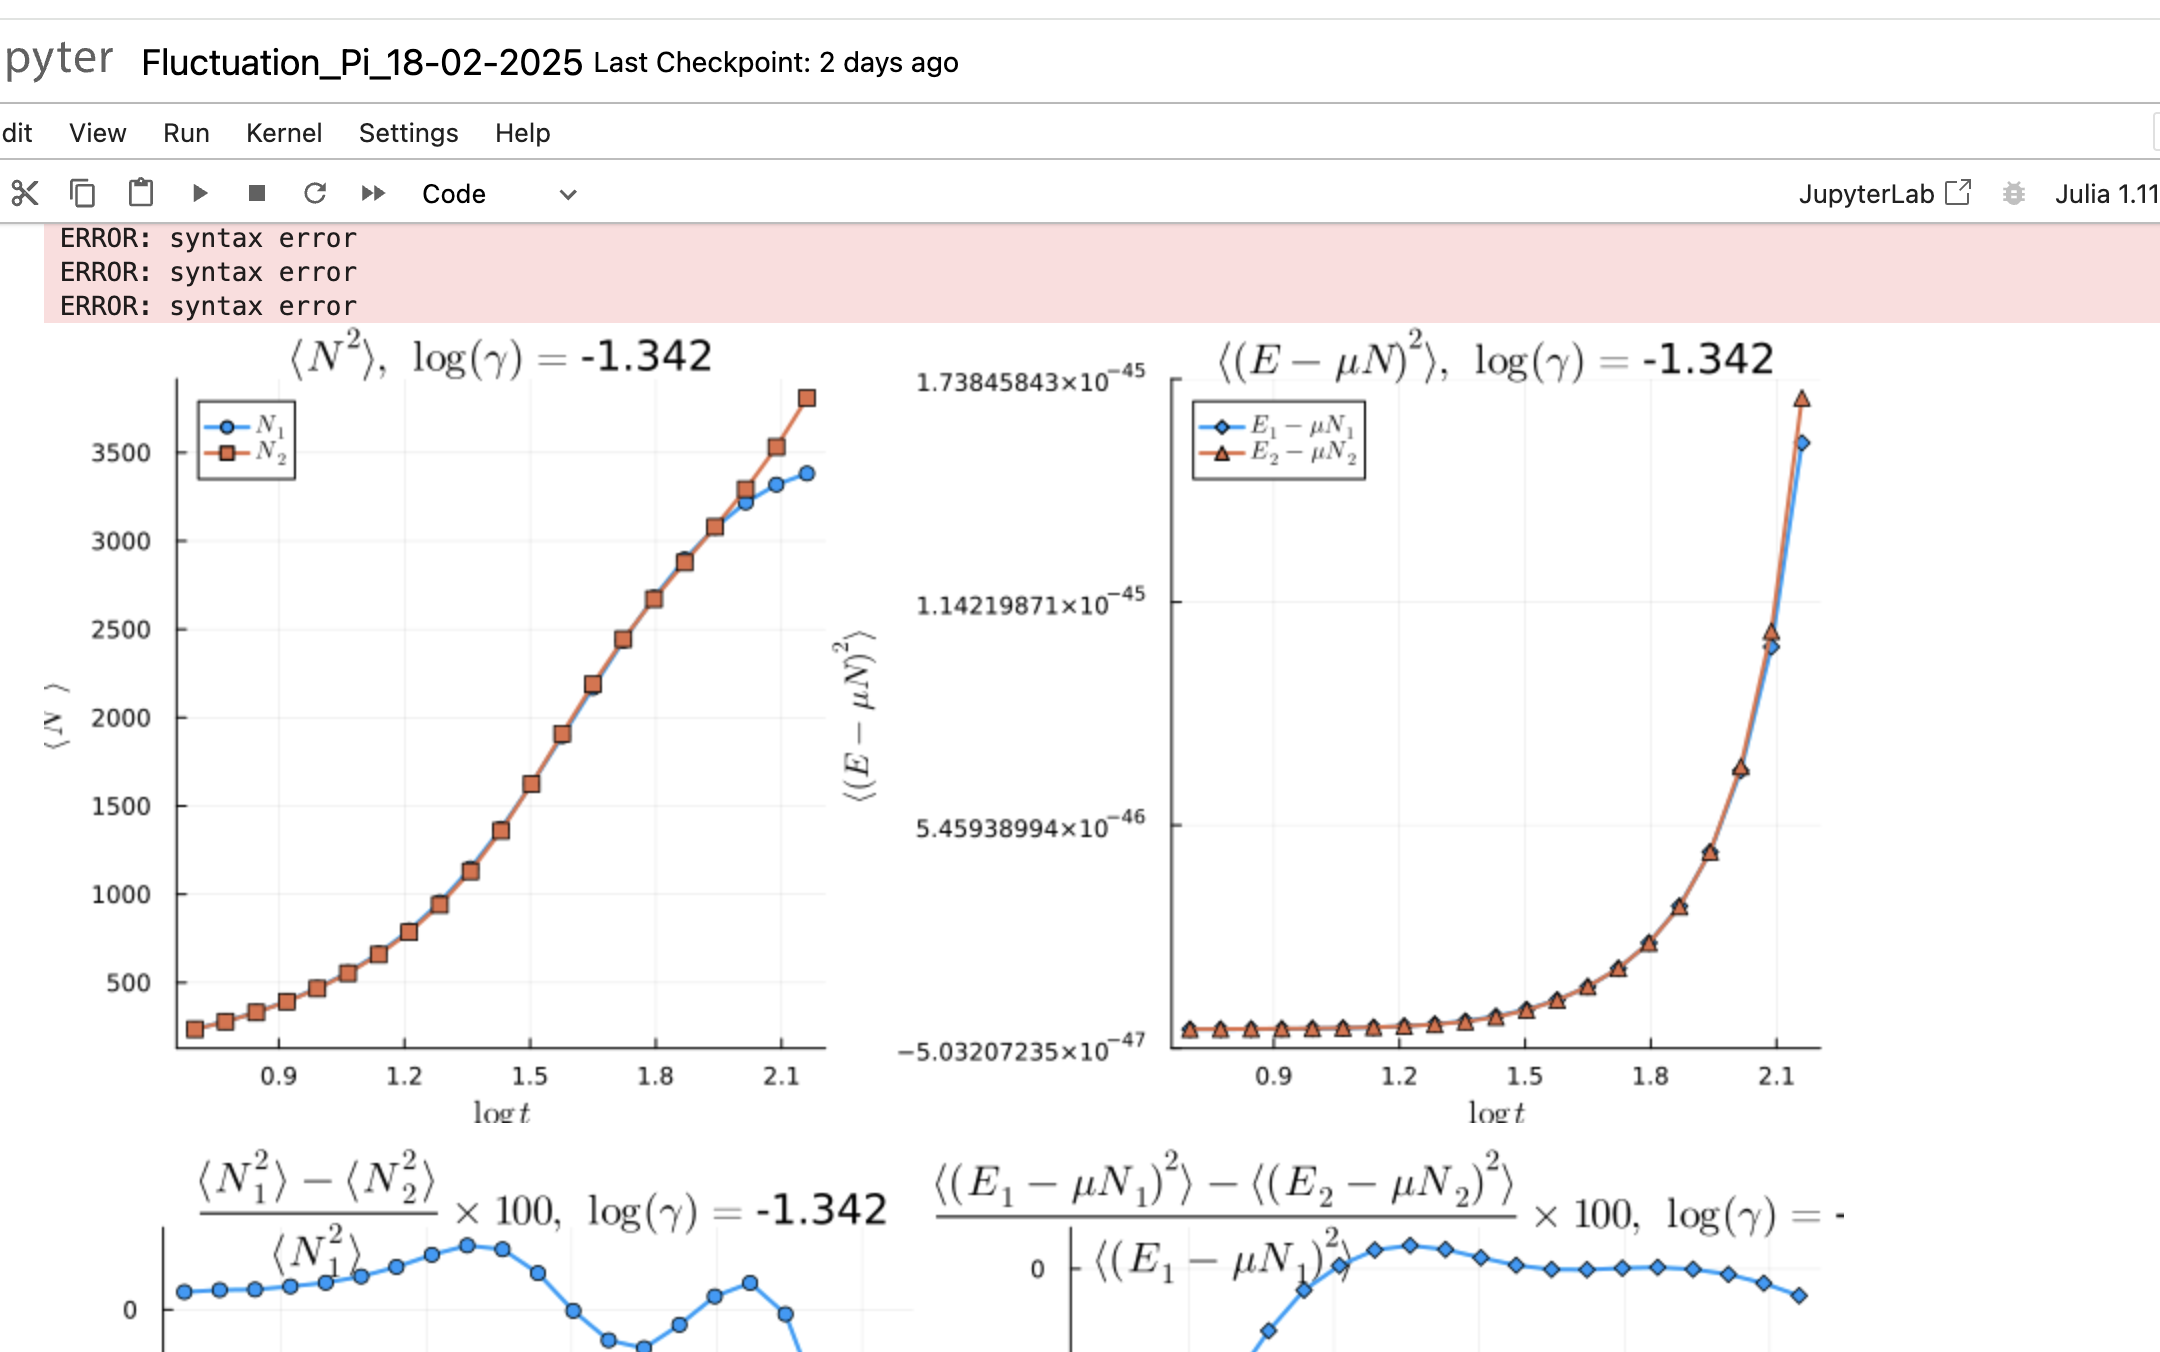
\includegraphics[width=1\textwidth]{Figures/test}

%\begin{aff}
%Donc une a l'ordre un en $\delta \theta (\operator{A}^{(0)})^{-1} %\operator{V}$ 

%\begin{eqnarray*}
%	\langle \delta \Pi ( \theta) \delta \Pi ( \theta') \rangle & = &  ( (\Pi^c_s - \Pi^c)\Pi^c/\Pi^c_s ) ( \theta ) \delta_{\theta, \theta'}/\delta \theta + \mathscr{F}(\theta , \theta' ) ,	
%\end{eqnarray*}

%avec 

%\begin{eqnarray*}
%	\mathscr{F}(\theta , \theta' ) & = & \left [ (\Pi^c_s - \Pi^c )( \theta)  +  (\Pi^c_s - \Pi^c ) ( \theta' )\right ] \frac{\Pi^c}{\Pi^c_s}(\theta)\frac{\Pi^c}{\Pi^c_s}(\theta') \frac{ \Delta( \theta'- \theta )}{ 2 \pi }\\
%	&&  - \left [ (\Pi^c_s - \Pi^c )( \theta)   (\Pi^c_s - \Pi^c ) ( \theta' )\right ] \frac{\Pi^c}{\Pi^c_s}(\theta)\frac{\Pi^c}{\Pi^c_s}(\theta')\int d\theta'' \left (   \frac{ \Pi^c/\Pi^c_s}{\Pi^c_s - \Pi^c} \right )(\theta'') \frac{\Delta(\theta''- \theta)}{2 \pi}\frac{\Delta(\theta''- \theta')}{2 \pi}  	
%\end{eqnarray*}
%\end{aff}



 










%\subsection{États du vide et pseudovacuum}
%%Dans ce chapitre, nous nous intéressons aux fluctuations de la distribution de rapidité \( \delta \rho \) autour d'une distribution de référence \( \rho^c \), qui maximise la contribution à la fonction de partition des états, exprimée comme une fonctionnelle de la distribution \( \rho \) : 

La fonction de partition des états, s'exprime comme une fonctionnelle de la distribution \( \rho \) : 

\begin{eqnarray*}
	\Xi & = & \sum_\rho \exp \left( -\mathcal{A}(\rho) \right).
\end{eqnarray*}  

Dans la section {\em \bf Entropie de Yang-Yang} (\ref{??}), l'action \( \mathcal{A}(\rho) \) s'écrit sous la forme :  

\begin{eqnarray*}
	\mathcal{A}(\rho) & \doteq & - L\mathcal{S}_{YY}(\rho) + L\int f(\theta) \rho (\theta) \, d\theta,		
\end{eqnarray*}  

où \( \mathcal{S}_{YY} \) est la fonctionnelle d'entropie de Yang-Yang, définie dans (\ref{??}), et \( f \) est la fonction paramétrant les charges, introduite dans (\ref{??}).  

Dans cette même section {\em \bf Entropie de Yang-Yang} (\ref{??}), nous avons établi un lien entre \( f \) et distribution de référence \( \rho^c \), qui maximise la contribution à la fonction de partition des états .\\

On veux tester si nos experience est décrit pas un GGE. Pour cela nous nous intéressons aux fluctuations de la distribution de rapidité \( \delta \rho \) autour \( \rho^c \).

%Nous poursuivons à présent avec cette définition de l'action de classe $\mathcal{C}^2$ et admetant une distribution critique $\rho^c$ tel que sa différentielle en ce point critique soit nulle $d\mathcal{A}_{\rho^c} = 0 $ (\ref{??}) de sorte que d'aprés la formule de Taylor-Youg %afin de déterminer les fluctuations autour de \( \Pi^c \). Pour cela, nous réécrivons l'action sous la forme :  

Nous poursuivons à présent avec cette définition de l'action de classe $\mathcal{C}^2$ et admetant une distribution critique $\rho^c$ tel que sa différentielle en ce point critique soit nulle $d\mathcal{A}_{\rho^c} = 0 $ (\ref{??}) de sorte que d'aprés la formule de Taylor-Youg %afin de déterminer les fluctuations autour de \( \Pi^c \). Pour cela, nous réécrivons l'action sous la forme :  

\begin{eqnarray*}  
	\mathcal{A}(\rho^c + \delta \rho) & \underset{ \delta \rho \to 0 }{=} & \mathcal{A}(\rho^c)  + \frac{1}{2} \left. \frac{\delta^2 \mathcal{A}}{\delta \rho^2} \right|_{\rho^c} (\delta \rho) + \mathcal{O}((\delta \rho)^3),  
\end{eqnarray*}  

une expression quadratique pour l'action à l'ordre dominant en \( \delta \Pi \) avec $\left. \frac{\delta^2 \mathcal{A}}{\delta \rho^2} \right|_{\rho^c}$ la forme quadratique définie positive (Fig (\ref{fig.fluctu.A})).

\begin{figure}[H]
	\centering 
	\begin{tikzpicture}
		\begin{scope}[shift={(0,0)}]
			\begin{scope}[transform canvas={scale=0.6}]
				% Définition des couleurs avec les codes HTML
\definecolor{colorOne}{HTML}{443E46}
\definecolor{colorTwo}{HTML}{F6DEB8}
\definecolor{colorThree}{HTML}{908CA4}
\definecolor{colorFour}{HTML}{57659E}
\definecolor{colorFive}{HTML}{C57284}
\definecolor{colorSix}{HTML}{FF5B69}

% Raccourcis pour les couleurs
\def\colorOne{colorOne}
\def\colorTwo{colorTwo}
\def\colorThree{colorThree}
\def\colorFour{colorFour}
\def\colorFive{colorFive}
\def\colorSix{colorSix}

\def\colorslide{blue!50!black}



\begin{scope}
	% Tracer une courbe lisse entre des points
	\draw[shift={(0,0)} ,\colorOne]
		(-1 , 0 ) edge [thick,line width=0.8ex , ->,>=triangle 45  , \colorOne] node [pos = 1 , below ]{\huge$\rho$}( 5  , 0 )
	;
	\draw[shift={(0,0)}, color=\colorOne]
		(0, -1.0 ) edge [thick,line width=0.8ex , ->,>=triangle 45  ]node [pos=0.9,left=0.2cm ]{\huge$\mathcal{A}(\rho)$}( 0  , 5 )
	;
	\draw[]
		(2.5, 0.12 ) edge [thick,line width=0.8ex ,\colorThree ]node [pos=1,below  ]{\huge$\rho^c$} (2.5, -0.12 )	
	;
	
	\draw[]
		(2.5, -0.12 ) edge [thick,line width=0.4ex , dashed, \colorThree ] (2.5, 5.5 )
		(1.5, 1 ) edge [thick,line width=0.4ex , <->,>=triangle 45  , \colorThree ] (3.5, 1 )
		(-0.3,1) edge [thick,line width=0.4ex  , \colorThree ] node [pos=0,left ]{\huge$\mathcal{A}(\rho^c)$} (0.3, 1 )	
	;
    \draw[thick, line width=0.8ex , \colorFour] plot[smooth, tension=0.7] coordinates {
        (1, 5) (1.6 , 3 ) (2.5, 1) (3.5 , 3 )  (4, 5)
    };		
	
\end{scope}

	
			
			\end{scope}
			
			\draw[color = red , scale = 0.5 , draw = none  ] (-2 , -1) rectangle (5, 6) ; 	
		\end{scope}
		
		\begin{scope}[shift={(19,-1)}]
			\begin{scope}[transform canvas={scale=0.6}]
				% Définition des couleurs avec les codes HTML
\definecolor{colorOne}{HTML}{443E46}
\definecolor{colorTwo}{HTML}{F6DEB8}
\definecolor{colorThree}{HTML}{908CA4}
\definecolor{colorFour}{HTML}{57659E}
\definecolor{colorFive}{HTML}{C57284}
\definecolor{colorSix}{HTML}{FF5B69}

% Raccourcis pour les couleurs
\def\colorOne{colorOne}
\def\colorTwo{colorTwo}
\def\colorThree{colorThree}
\def\colorFour{colorFour}
\def\colorFive{colorFive}
\def\colorSix{colorSix}

\def\colorslide{blue!50!black}

\def\Occupation{
	\def\traitx{0.3}
	\def\traity{0.5}
	\draw[shift={(0,0)}]
		(-13.5 , 0 ) edge [thick,line width=0.8ex ]( -3.2  , 0 )
		( -3.2 - \traitx  , 0 - \traity ) edge [thick,line width=0.8ex ]( -3.2 + \traitx  , 0 + \traity  )
		( -2.8 - \traitx  , 0 - \traity ) edge [thick,line width=0.8ex ]( -2.8 + \traitx  , 0 + \traity  )
		(-2.8 , 0 ) edge [thick,line width=0.8ex ](2.8  , 0 )
		( 2.8 - \traitx  , 0 - \traity ) edge [thick,line width=0.8ex ]( 2.8 + \traitx  , 0 + \traity  )
		( 3.2 - \traitx  , 0 - \traity ) edge [thick,line width=0.8ex ]( 3.2 + \traitx  , 0 + \traity  )
		(3.2, 0 ) edge [thick,line width=0.8ex,->,>=triangle 45 , color = black ]node [pos=1.01,below  ]{\huge$\theta$}	( 13  , 0 )
	;
	\draw[shift={(0,0)}, color=\colorOne]
		(-10.5 , -1.5 ) edge [thick,line width=0.8ex , ->,>=triangle 45  ]( -10.5  , 4.5 )
	;
		
	\foreach \r in {1 , ... , 3 } {
%		\draw[
%		decoration={
%		markings,
%    	mark connection node=my node,
%    	mark=at position 0 with{\node [blue,transform shape] (my node) {\large \r};}},
%		color=gray, thick, 
%		line width=0.5ex] decorate { 
%            (-11.0, \r) -- (-10.1, \r )}
%        ;
        \draw[
			color=\colorOne,
			] 
            (-11.0, \r) edge[color=\colorThree , thick,line width=0.5ex] node [pos=-0.5 ]{\large\color{\colorFour} $\frac{\r}{\delta \theta}$ } (-10.3, \r )
        	;
	
	}
	

	
	% Graduation abcsisse 
	% Définitions des listes
% Definitions of the lists
\def\listetuple{-9/\theta_{1}, -8/\theta_{2} , -5/\theta_{3} , -2/\theta_{a-1} , 0/\theta_{a} , 1/\theta_{a+1} , 2/\theta_{a+2} ,  5/\theta_{N-4} , 7/\theta_{N-3},8/\theta_{N-1},9/\theta_{N} }
\def\listetrais{-12 , -11, -10, -9 , -8 , -7 ,  -6 , -5, -4.5,-4, -2 , -1, 0 , 0.5, 1, 2, 4 , 5 ,  6 , 7 , 8 ,8.5, 9 ,  10 , 11, 12 }

% Loop over listetrais
\foreach \r in \listetrais {
    % Initialize found variable to zero
    % Initialize found variable to zero
    %\pgfmathsetmacro\found{0}
    \global\def\found{0}
    \xdef\nomtheta{}
    
    % Check if \r is in listetuple
    \foreach \x/\y in \listetuple { 
        \ifdim \r pt=\x pt % If \r matches any \x in listetuple
            \global\def\found{1} ;
            \xdef\nomtheta{\y} % Set \nomtheta to the corresponding \y
            %\pgfmathsetmacro\found{1} % Set found to 1            
            %\global\pgfmathsetmacro\found{1}
        \fi
    }
    
    %\node [circle, draw, red] (A) at (\r, 2) {\found , $\nomtheta$};
    
    % Draw the line and display \nomtheta if found
    \ifnum\found=1
        \draw[color=\colorOne, thick, line width=0.5ex] 
            (\r, -0.3) -- (\r, 0.3) node[red , pos=-0.5] {\large $\nomtheta$};
         \filldraw[line width=0.5ex, color=\colorSix, outer color=\colorSix, inner color=\colorSix] 
            (\r, 0) circle (4pt);
    \else 
        % Draw without \nomtheta and add a blue circle if not found
        \draw[color=\colorOne, thick, line width=0.5ex] 
            (\r, -0.3) -- (\r, 0.3);
        \filldraw[line width=0.5ex, color=\colorSix, outer color=\colorTwo, inner color=\colorTwo] 
            (\r, 0) circle (4pt); 
    \fi
}

\def\listetrais{-9.5/\theta_{i-1}/2/3, -6.5/\theta_{i}/1/4  ,   -1.5/\theta_{j}/2/4 , 1.5/\theta_{j+1}/-1/3 , 3.5/\theta_{\ell-1}/1/3 , 6.5/\theta_{\ell}/3/4 , 9.5/\theta(\theta_{\ell+1})/-1/3 };



\foreach \r/\nomx/\y/\ys in \listetrais {
	\draw[
		decoration={
		markings,
    	mark connection node=my node,
    	mark=at position .5 with{\node [blue,transform shape] (my node) {\large \color{\colorFour} $\nomx$};}},
		color=\colorThree , thick, 
		line width=0.5ex] decorate { 
            (\r, 0.12) -- (\r, -1.2)}
        ;
     
     \ifdim \y pt > -1 pt 
     	\draw[
			decoration={
			markings,
    		mark connection node=my node,
    		mark=at position .5 with{\node [blue,transform shape] (my node) {\large \color{\colorFour} $\Pi(\nomx) $};}},
			color=\colorThree, thick, 
			line width=0.5ex] decorate { 
            (\r, \y) -- (\r +3, \y)}
        ;
        \draw[
			decoration={
			markings,
    		mark connection node=my node,
    		mark=at position .5 with{\node [blue,transform shape] (my node) {\large \color{\colorFive} $\Pi_s(\nomx) $};}},
			color=\colorFive, thick, 
			line width=0.5ex] decorate { 
            (\r, \ys) -- (\r +3, \ys)}
        ;
     \fi 
     \ifdim \r pt= -1.5 pt
     	\draw[
     		decoration={
			markings,
    		mark connection node=my node,
    		mark=at position .5 with{\node [blue,transform shape] (my node) {\large \color{\colorFour}  $\delta \theta $};},
    		%mark=at position 0.1  with {\arrow[blue, line width=0.5ex]{<}},
    		%mark=at position 1  with {\arrow[blue, line width=0.5ex]{>}}
    		},
        	color=\colorThree,
        	thick,
        	line width=0.5ex,
        	%arrows={Computer Modern Rightarrow[line cap=round]-Computer Modern Rightarrow[line cap=round]}
   			](\r, -1.2) edge[arrows={Computer Modern Rightarrow[line cap=round]-}] (\r + 0.4, -1.2)decorate {
    		(\r, -1.2) -- (\r + 3, -1.2)}(\r + 2, -1.2) edge[arrows={-Computer Modern Rightarrow[line cap=round]}] (\r + 3, -1.2)
    		;
    \fi
			
	
}


			
}


\begin{scope}
	%\draw[help lines , width=1.5ex] (-8,-3) grid (8,3);\draw[help lines ,width=0.5ex , opacity = 0.5] (-3,-3) grid[step=0.1] (3,3));
	
	%\draw[help lines] 
	%	(-3,-3) edge[width=1.5ex] grid (3,3)	
	%	(-3,-3) edge[width=0.5ex , opacity = 0.5] grid (3,3)	
	%;
	\begin{scope}[shift={(0,1)},rotate=0,opacity=1,color=black]
		\Occupation	
		
		%\node[anchor=east, font=\bfseries] at (-11, 0) {\color{red}\large (T = 0 )} ;	
	\end{scope}
	
	
	
	
	\begin{scope}[shift={(-10.5,7)},rotate=0,opacity=1,color=black]
	
	\begin{scope}[shift={(-0,0)},rotate=0,opacity=1,color=black]
	
		\draw[shift={(0,0)} ,line width=1ex,rounded corners = 1ex,color=\colorOne , opacity =1 ,fill=\colorOne!00 , pattern={north east lines} , pattern color=\colorOne!00 ]
			(0 , -1 ) rectangle (5,1)
		;
		

		\begin{scope}[shift={(0.5,0.5)}]
			\draw[color=\colorOne, thick, line width=0.5ex] 
            (0, -0.3) -- (0, 0.3) ;
            \filldraw[line width=0.5ex, color=\colorSix, outer color=\colorSix, inner color=\colorSix] 
            (0, 0) circle (4pt);
            
            \node[anchor=west, font=\bfseries] at (0.2, 0) {\color{\colorSix}\large : quasi-particule};
		\end{scope}
		
		\begin{scope}[shift={(0.5,-0.5)}]
			\draw[color=\colorOne, thick, line width=0.5ex] 
            (0, -0.3) -- (0, 0.3) ;
            \filldraw[line width=0.5ex, color=\colorSix, outer color=\colorTwo, inner color=\colorTwo] 
            (0, 0) circle (4pt);
            
            \node[anchor=west, font=\bfseries] at (0.2, 0) {\color{\colorSix}\large : hole};
		\end{scope}

	\end{scope}
	
	\begin{scope}[shift={(6,0)},rotate=0,opacity=1,color=black]	
		
		\draw[shift={(0,0)} ,line width=1ex,rounded corners = 1ex,color=\colorOne , opacity =1 ,fill=\colorOne!00 , pattern={north east lines} , pattern color=\colorOne!00 ]
			(0 , -1 ) rectangle (7.5,1)
		;
		
		\node[anchor=west] at (0.5, 0.5) {\color{\colorFour}\large $\Pi$ };\node[anchor=west, font=\bfseries] at (1, 0.5) {\color{\colorFour}\large : quasi-particule distribution};
		
		\node[anchor=west] at (0.5, -0.5) {\color{\colorFour}\large $\Pi_h$ };\node[anchor=west, font=\bfseries] at (1, -0.5) {\color{\colorFour}\large  : hole distribution};
		
	\end{scope}
	
	\begin{scope}[shift={(14.5,0)},rotate=0,opacity=1,color=black]	
		
		\draw[shift={(0,0)} ,line width=1ex,rounded corners = 1ex,color=\colorOne , opacity =1 ,fill=\colorOne!00 , pattern={north east lines} , pattern color=\colorOne!00 ]
			(0 , -0.5 ) rectangle (7.0,0.5)
		;
		
		\node[anchor=west] at (0.2, 0) {\color{\colorFour}\large ${\color{\colorFive}\Pi_s} = \Pi + \Pi_h $ } node[anchor=west , font=\bfseries] at (3.1 , 0 )  {\color{\colorFour}\large {\color{\colorFive} : density of states}};
		
	\end{scope}
	
	
	\end{scope}


		
	
\end{scope}

	
			
			\end{scope}
			\begin{scope}[scale=1]
				\draw[color = red , scale = 1 , draw = none  ] (-1 , -1) rectangle (5, 5) ; 
			\end{scope}	
		\end{scope}

		
				
			
	\end{tikzpicture}	
	\captionsetup{skip=10pt} % Ajoute de l’espace après la légende
	\label{fig.fluctu.A}
\end{figure}


On discrétise l'axe des rapidités en  petite cellule de rapidité $[\theta, \theta+\delta\theta]$, qui contient $L\rho(\theta) \delta \theta$ rapidités. 
	



Avec ces petites tranches, la forme quadratique s’écrit :

\begin{eqnarray*}
    \left. \frac{\delta^2 \mathcal{A}}{{\delta \rho}^2} \right|_{\rho^c}(\delta \rho ) &=&  \sum_{a,b \mid \text{tranche}}  
    \delta \rho(\theta_a)  \frac{\partial^2 \mathcal{A}}{\partial \delta \rho(\theta_a) \partial \delta \rho(\theta_b) } (\rho^c)  \delta \rho(\theta_b).
\end{eqnarray*}
Les fluctuations s’écrivent donc :

\begin{eqnarray*}
    \langle \delta \rho ( \theta) \delta \rho ( \theta') \rangle &=&  
    \frac{ \int d\delta \rho \, \delta \rho(\theta) \delta \rho ( \theta') 
    \exp \left( - \frac{1}{2} \sum_{a,b \mid \text{tranche}}  
    \delta \rho(\theta_a) \frac{\partial^2 \mathcal{A}}{\partial \delta \rho(\theta_a) \partial \delta \rho(\theta_b) } (\rho^c)  \delta \rho(\theta_b) \right) }
    { \int d\delta \Pi  
    \exp \left( - \frac{1}{2} \sum_{a,b \mid \text{tranche}}  
    \delta \rho(\theta_a) \frac{\partial^2 \mathcal{A}}{\partial \delta \rho(\theta_a) \partial \delta \rho(\theta_b) } (\rho^c)  \delta \rho(\theta_b) \right) } \\
    &=& \left( \mathbf{A}^{-1} \right)_{\theta , \theta'}
\end{eqnarray*}


\begin{aff}

\begin{eqnarray*}
	\langle \delta \rho ( \theta) \delta \rho ( \theta') \rangle &=& 	\left( \mathbf{A}^{-1} \right)_{\theta , \theta'}
\end{eqnarray*}

	
avec la  {\em matrice hessienne} $\mathbf{A}_{\theta , \theta'} \equiv \frac{\partial^2 \mathcal{A}}{\partial \delta \rho(\theta) \partial \delta \rho(\theta') }(\rho^c)$, au point critique/ qui maximise la probabilité  $\rho^c=\rho^c_s \nu^c $, s'écrit

\begin{eqnarray*}
	\operator{A} & = & \operator{A}^{(0)} + \delta \theta \operator{V}
\end{eqnarray*}

avec 

\begin{eqnarray*}
	A^{(0)}_{\theta , \theta'}  & = &  L\delta \theta \left ( \frac{ 1}{\rho^c_s ( 1  - \nu^c ) \nu^c } \right )(\theta)    \delta({\theta - \theta '})	,\\
	V_{\theta , \theta'}  &= & L \delta \theta \left \{ - \left [ \left ( \frac{1}{\rho^c_s( 1 - \nu^c) } \right ) ( \theta)  +  \left ( \frac{1}{\rho^c_s( 1 - \nu^c) } \right ) ( \theta' )\right ] \frac{ \Delta( \theta'- \theta )}{ 2 \pi } + \int d\theta''  \left ( \frac{\nu^c}{\rho^c_s( 1 - \nu^c) } \right )(\theta'') \frac{\Delta(\theta''- \theta)}{2 \pi}\frac{\Delta(\theta''- \theta')}{2 \pi}   \right \} 	
\end{eqnarray*}

\end{aff}

\subsection{Testes}

\begin{eqnarray*}
	\Delta_{\operator{\mathcal{N}}}^2  & = &  \frac{1}{\beta} \left . \frac{\partial \langle \operator{\mathcal{N}} \rangle}{\partial \mu} \right )_T \\
	\Delta_{\operator{\mathcal{E}}-\mu \operator{\mathcal{N}}}^2  & = &  - \left . \frac{\partial \langle \operator{\mathcal{E}}-\mu \operator{\mathcal{N}} \rangle}{\partial \beta} \right )_\mu 
\end{eqnarray*}

et 

\begin{eqnarray*}
	\Delta_{\operator{\mathcal{N}}}^2  &= & L^2 \int d\theta_a \int d \theta_b \, \langle \delta \rho(\theta_a) \delta \rho(\theta_b) \rangle \\
	\Delta_{\operator{\mathcal{E}}-\mu \operator{\mathcal{N}}}^2  & = & L^2 \int d\theta_a \int d \theta_b \, \left ( - \mu + \frac{1}2 m \theta_a^2  \right  )\left ( - \mu + \frac{1}2 m \theta_b^2  \right  )  \langle \delta \rho(\theta_a) \delta \rho(\theta_b) \rangle
\end{eqnarray*}

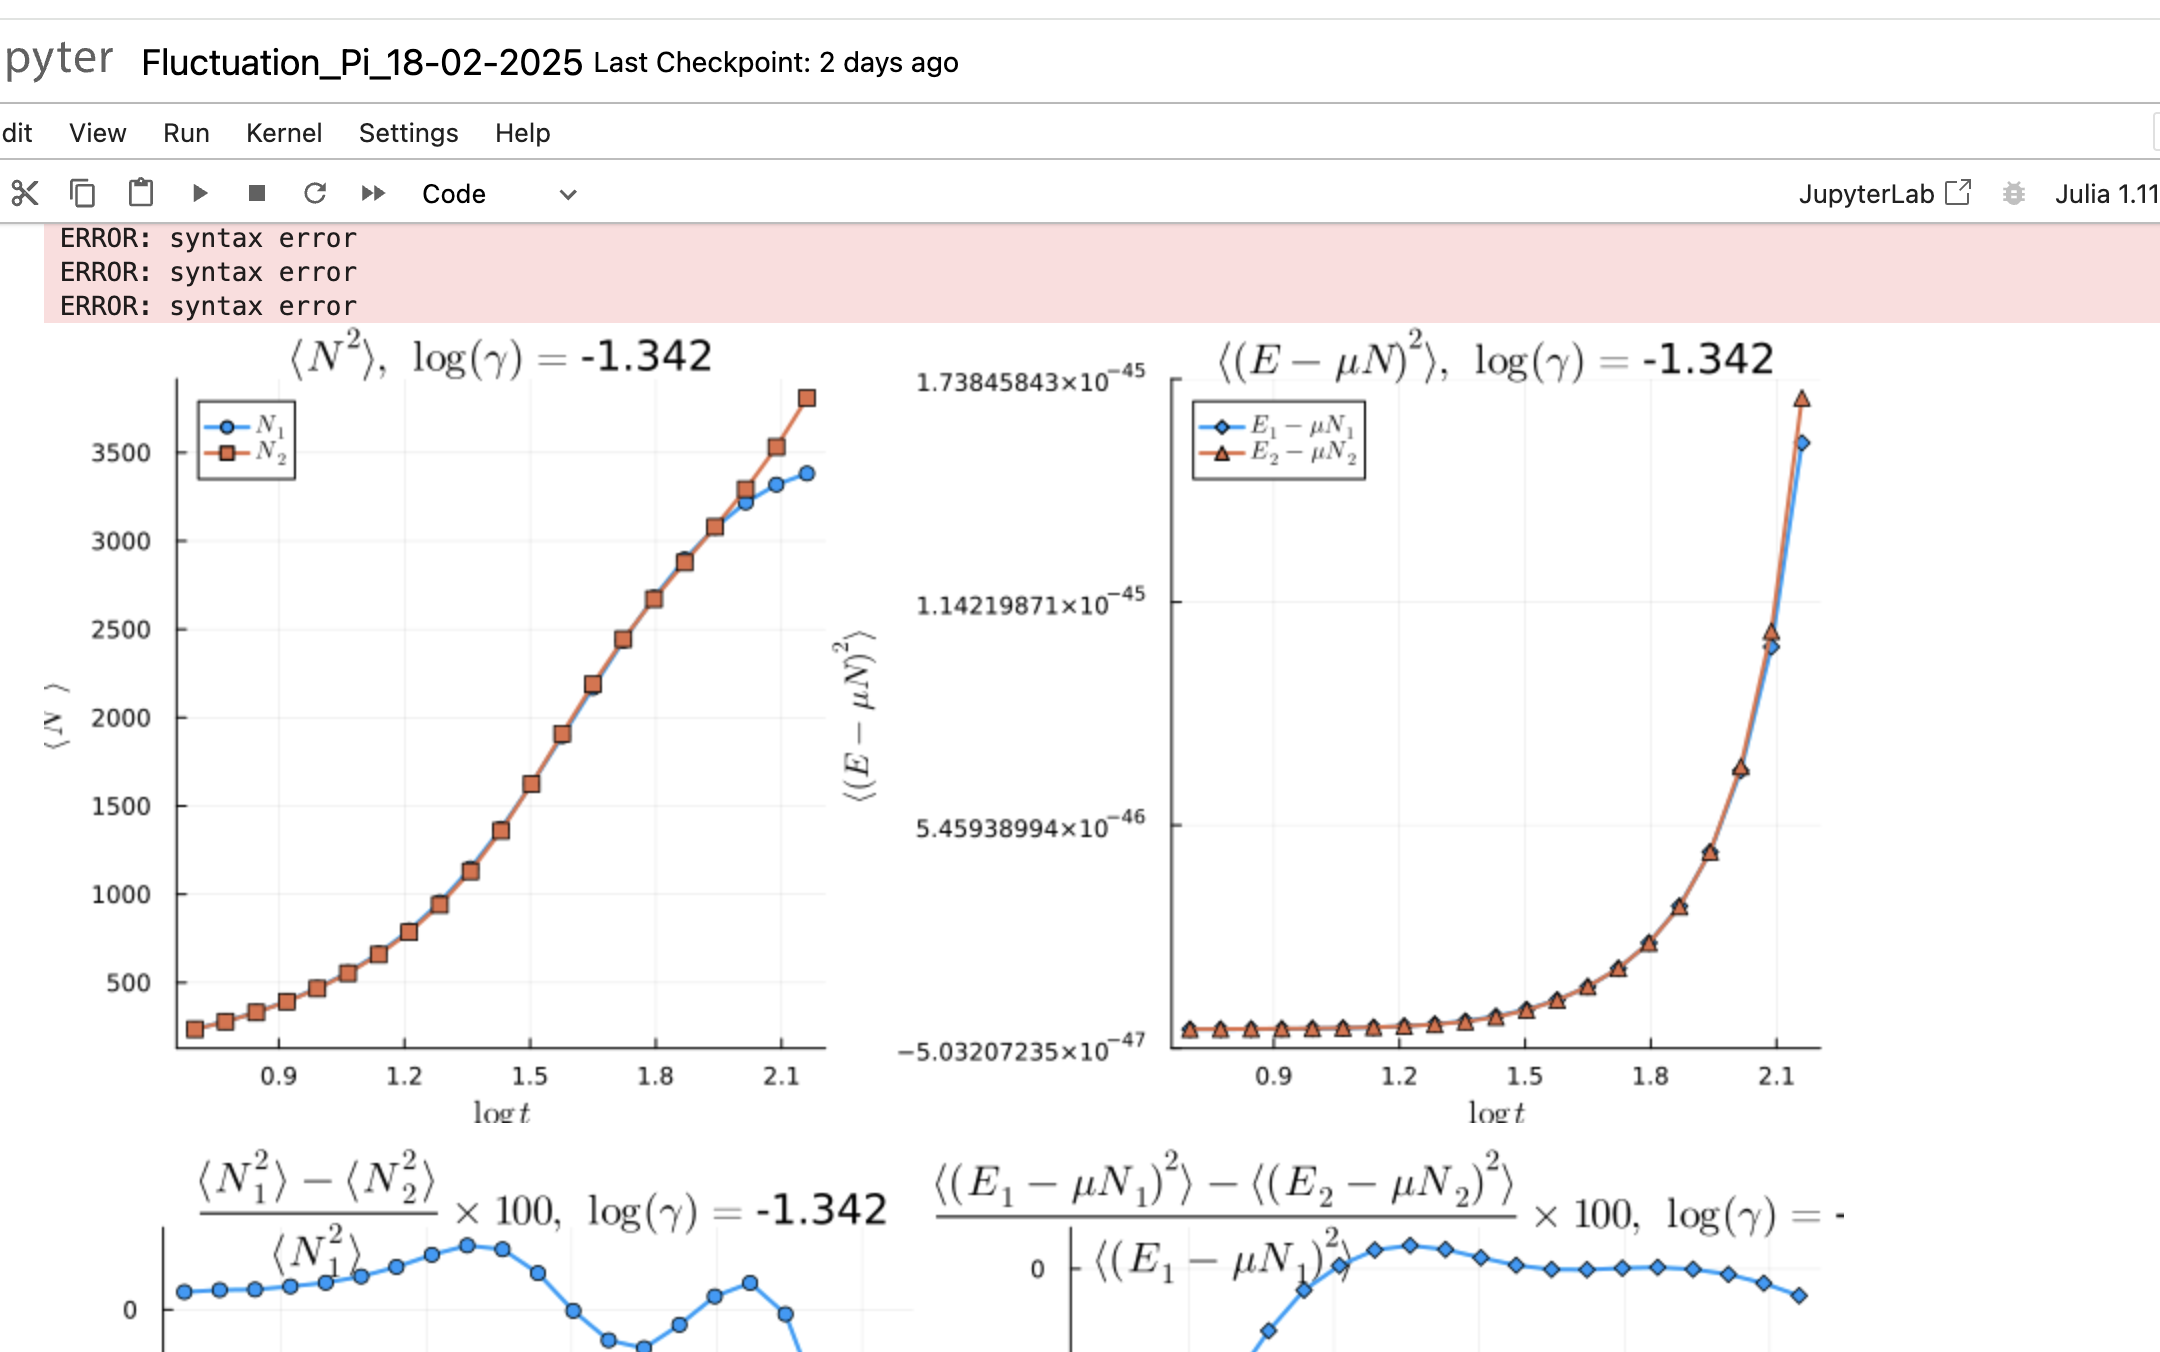
\includegraphics[width=1\textwidth]{Figures/test}

%\begin{aff}
%Donc une a l'ordre un en $\delta \theta (\operator{A}^{(0)})^{-1} %\operator{V}$ 

%\begin{eqnarray*}
%	\langle \delta \Pi ( \theta) \delta \Pi ( \theta') \rangle & = &  ( (\Pi^c_s - \Pi^c)\Pi^c/\Pi^c_s ) ( \theta ) \delta_{\theta, \theta'}/\delta \theta + \mathscr{F}(\theta , \theta' ) ,	
%\end{eqnarray*}

%avec 

%\begin{eqnarray*}
%	\mathscr{F}(\theta , \theta' ) & = & \left [ (\Pi^c_s - \Pi^c )( \theta)  +  (\Pi^c_s - \Pi^c ) ( \theta' )\right ] \frac{\Pi^c}{\Pi^c_s}(\theta)\frac{\Pi^c}{\Pi^c_s}(\theta') \frac{ \Delta( \theta'- \theta )}{ 2 \pi }\\
%	&&  - \left [ (\Pi^c_s - \Pi^c )( \theta)   (\Pi^c_s - \Pi^c ) ( \theta' )\right ] \frac{\Pi^c}{\Pi^c_s}(\theta)\frac{\Pi^c}{\Pi^c_s}(\theta')\int d\theta'' \left (   \frac{ \Pi^c/\Pi^c_s}{\Pi^c_s - \Pi^c} \right )(\theta'') \frac{\Delta(\theta''- \theta)}{2 \pi}\frac{\Delta(\theta''- \theta')}{2 \pi}  	
%\end{eqnarray*}
%\end{aff}



 










%\subsection{Opérateurs conservés (intégrales du mouvement)}
%%Dans ce chapitre, nous nous intéressons aux fluctuations de la distribution de rapidité \( \delta \rho \) autour d'une distribution de référence \( \rho^c \), qui maximise la contribution à la fonction de partition des états, exprimée comme une fonctionnelle de la distribution \( \rho \) : 

La fonction de partition des états, s'exprime comme une fonctionnelle de la distribution \( \rho \) : 

\begin{eqnarray*}
	\Xi & = & \sum_\rho \exp \left( -\mathcal{A}(\rho) \right).
\end{eqnarray*}  

Dans la section {\em \bf Entropie de Yang-Yang} (\ref{??}), l'action \( \mathcal{A}(\rho) \) s'écrit sous la forme :  

\begin{eqnarray*}
	\mathcal{A}(\rho) & \doteq & - L\mathcal{S}_{YY}(\rho) + L\int f(\theta) \rho (\theta) \, d\theta,		
\end{eqnarray*}  

où \( \mathcal{S}_{YY} \) est la fonctionnelle d'entropie de Yang-Yang, définie dans (\ref{??}), et \( f \) est la fonction paramétrant les charges, introduite dans (\ref{??}).  

Dans cette même section {\em \bf Entropie de Yang-Yang} (\ref{??}), nous avons établi un lien entre \( f \) et distribution de référence \( \rho^c \), qui maximise la contribution à la fonction de partition des états .\\

On veux tester si nos experience est décrit pas un GGE. Pour cela nous nous intéressons aux fluctuations de la distribution de rapidité \( \delta \rho \) autour \( \rho^c \).

%Nous poursuivons à présent avec cette définition de l'action de classe $\mathcal{C}^2$ et admetant une distribution critique $\rho^c$ tel que sa différentielle en ce point critique soit nulle $d\mathcal{A}_{\rho^c} = 0 $ (\ref{??}) de sorte que d'aprés la formule de Taylor-Youg %afin de déterminer les fluctuations autour de \( \Pi^c \). Pour cela, nous réécrivons l'action sous la forme :  

Nous poursuivons à présent avec cette définition de l'action de classe $\mathcal{C}^2$ et admetant une distribution critique $\rho^c$ tel que sa différentielle en ce point critique soit nulle $d\mathcal{A}_{\rho^c} = 0 $ (\ref{??}) de sorte que d'aprés la formule de Taylor-Youg %afin de déterminer les fluctuations autour de \( \Pi^c \). Pour cela, nous réécrivons l'action sous la forme :  

\begin{eqnarray*}  
	\mathcal{A}(\rho^c + \delta \rho) & \underset{ \delta \rho \to 0 }{=} & \mathcal{A}(\rho^c)  + \frac{1}{2} \left. \frac{\delta^2 \mathcal{A}}{\delta \rho^2} \right|_{\rho^c} (\delta \rho) + \mathcal{O}((\delta \rho)^3),  
\end{eqnarray*}  

une expression quadratique pour l'action à l'ordre dominant en \( \delta \Pi \) avec $\left. \frac{\delta^2 \mathcal{A}}{\delta \rho^2} \right|_{\rho^c}$ la forme quadratique définie positive (Fig (\ref{fig.fluctu.A})).

\begin{figure}[H]
	\centering 
	\begin{tikzpicture}
		\begin{scope}[shift={(0,0)}]
			\begin{scope}[transform canvas={scale=0.6}]
				% Définition des couleurs avec les codes HTML
\definecolor{colorOne}{HTML}{443E46}
\definecolor{colorTwo}{HTML}{F6DEB8}
\definecolor{colorThree}{HTML}{908CA4}
\definecolor{colorFour}{HTML}{57659E}
\definecolor{colorFive}{HTML}{C57284}
\definecolor{colorSix}{HTML}{FF5B69}

% Raccourcis pour les couleurs
\def\colorOne{colorOne}
\def\colorTwo{colorTwo}
\def\colorThree{colorThree}
\def\colorFour{colorFour}
\def\colorFive{colorFive}
\def\colorSix{colorSix}

\def\colorslide{blue!50!black}



\begin{scope}
	% Tracer une courbe lisse entre des points
	\draw[shift={(0,0)} ,\colorOne]
		(-1 , 0 ) edge [thick,line width=0.8ex , ->,>=triangle 45  , \colorOne] node [pos = 1 , below ]{\huge$\rho$}( 5  , 0 )
	;
	\draw[shift={(0,0)}, color=\colorOne]
		(0, -1.0 ) edge [thick,line width=0.8ex , ->,>=triangle 45  ]node [pos=0.9,left=0.2cm ]{\huge$\mathcal{A}(\rho)$}( 0  , 5 )
	;
	\draw[]
		(2.5, 0.12 ) edge [thick,line width=0.8ex ,\colorThree ]node [pos=1,below  ]{\huge$\rho^c$} (2.5, -0.12 )	
	;
	
	\draw[]
		(2.5, -0.12 ) edge [thick,line width=0.4ex , dashed, \colorThree ] (2.5, 5.5 )
		(1.5, 1 ) edge [thick,line width=0.4ex , <->,>=triangle 45  , \colorThree ] (3.5, 1 )
		(-0.3,1) edge [thick,line width=0.4ex  , \colorThree ] node [pos=0,left ]{\huge$\mathcal{A}(\rho^c)$} (0.3, 1 )	
	;
    \draw[thick, line width=0.8ex , \colorFour] plot[smooth, tension=0.7] coordinates {
        (1, 5) (1.6 , 3 ) (2.5, 1) (3.5 , 3 )  (4, 5)
    };		
	
\end{scope}

	
			
			\end{scope}
			
			\draw[color = red , scale = 0.5 , draw = none  ] (-2 , -1) rectangle (5, 6) ; 	
		\end{scope}
		
		\begin{scope}[shift={(19,-1)}]
			\begin{scope}[transform canvas={scale=0.6}]
				% Définition des couleurs avec les codes HTML
\definecolor{colorOne}{HTML}{443E46}
\definecolor{colorTwo}{HTML}{F6DEB8}
\definecolor{colorThree}{HTML}{908CA4}
\definecolor{colorFour}{HTML}{57659E}
\definecolor{colorFive}{HTML}{C57284}
\definecolor{colorSix}{HTML}{FF5B69}

% Raccourcis pour les couleurs
\def\colorOne{colorOne}
\def\colorTwo{colorTwo}
\def\colorThree{colorThree}
\def\colorFour{colorFour}
\def\colorFive{colorFive}
\def\colorSix{colorSix}

\def\colorslide{blue!50!black}

\def\Occupation{
	\def\traitx{0.3}
	\def\traity{0.5}
	\draw[shift={(0,0)}]
		(-13.5 , 0 ) edge [thick,line width=0.8ex ]( -3.2  , 0 )
		( -3.2 - \traitx  , 0 - \traity ) edge [thick,line width=0.8ex ]( -3.2 + \traitx  , 0 + \traity  )
		( -2.8 - \traitx  , 0 - \traity ) edge [thick,line width=0.8ex ]( -2.8 + \traitx  , 0 + \traity  )
		(-2.8 , 0 ) edge [thick,line width=0.8ex ](2.8  , 0 )
		( 2.8 - \traitx  , 0 - \traity ) edge [thick,line width=0.8ex ]( 2.8 + \traitx  , 0 + \traity  )
		( 3.2 - \traitx  , 0 - \traity ) edge [thick,line width=0.8ex ]( 3.2 + \traitx  , 0 + \traity  )
		(3.2, 0 ) edge [thick,line width=0.8ex,->,>=triangle 45 , color = black ]node [pos=1.01,below  ]{\huge$\theta$}	( 13  , 0 )
	;
	\draw[shift={(0,0)}, color=\colorOne]
		(-10.5 , -1.5 ) edge [thick,line width=0.8ex , ->,>=triangle 45  ]( -10.5  , 4.5 )
	;
		
	\foreach \r in {1 , ... , 3 } {
%		\draw[
%		decoration={
%		markings,
%    	mark connection node=my node,
%    	mark=at position 0 with{\node [blue,transform shape] (my node) {\large \r};}},
%		color=gray, thick, 
%		line width=0.5ex] decorate { 
%            (-11.0, \r) -- (-10.1, \r )}
%        ;
        \draw[
			color=\colorOne,
			] 
            (-11.0, \r) edge[color=\colorThree , thick,line width=0.5ex] node [pos=-0.5 ]{\large\color{\colorFour} $\frac{\r}{\delta \theta}$ } (-10.3, \r )
        	;
	
	}
	

	
	% Graduation abcsisse 
	% Définitions des listes
% Definitions of the lists
\def\listetuple{-9/\theta_{1}, -8/\theta_{2} , -5/\theta_{3} , -2/\theta_{a-1} , 0/\theta_{a} , 1/\theta_{a+1} , 2/\theta_{a+2} ,  5/\theta_{N-4} , 7/\theta_{N-3},8/\theta_{N-1},9/\theta_{N} }
\def\listetrais{-12 , -11, -10, -9 , -8 , -7 ,  -6 , -5, -4.5,-4, -2 , -1, 0 , 0.5, 1, 2, 4 , 5 ,  6 , 7 , 8 ,8.5, 9 ,  10 , 11, 12 }

% Loop over listetrais
\foreach \r in \listetrais {
    % Initialize found variable to zero
    % Initialize found variable to zero
    %\pgfmathsetmacro\found{0}
    \global\def\found{0}
    \xdef\nomtheta{}
    
    % Check if \r is in listetuple
    \foreach \x/\y in \listetuple { 
        \ifdim \r pt=\x pt % If \r matches any \x in listetuple
            \global\def\found{1} ;
            \xdef\nomtheta{\y} % Set \nomtheta to the corresponding \y
            %\pgfmathsetmacro\found{1} % Set found to 1            
            %\global\pgfmathsetmacro\found{1}
        \fi
    }
    
    %\node [circle, draw, red] (A) at (\r, 2) {\found , $\nomtheta$};
    
    % Draw the line and display \nomtheta if found
    \ifnum\found=1
        \draw[color=\colorOne, thick, line width=0.5ex] 
            (\r, -0.3) -- (\r, 0.3) node[red , pos=-0.5] {\large $\nomtheta$};
         \filldraw[line width=0.5ex, color=\colorSix, outer color=\colorSix, inner color=\colorSix] 
            (\r, 0) circle (4pt);
    \else 
        % Draw without \nomtheta and add a blue circle if not found
        \draw[color=\colorOne, thick, line width=0.5ex] 
            (\r, -0.3) -- (\r, 0.3);
        \filldraw[line width=0.5ex, color=\colorSix, outer color=\colorTwo, inner color=\colorTwo] 
            (\r, 0) circle (4pt); 
    \fi
}

\def\listetrais{-9.5/\theta_{i-1}/2/3, -6.5/\theta_{i}/1/4  ,   -1.5/\theta_{j}/2/4 , 1.5/\theta_{j+1}/-1/3 , 3.5/\theta_{\ell-1}/1/3 , 6.5/\theta_{\ell}/3/4 , 9.5/\theta(\theta_{\ell+1})/-1/3 };



\foreach \r/\nomx/\y/\ys in \listetrais {
	\draw[
		decoration={
		markings,
    	mark connection node=my node,
    	mark=at position .5 with{\node [blue,transform shape] (my node) {\large \color{\colorFour} $\nomx$};}},
		color=\colorThree , thick, 
		line width=0.5ex] decorate { 
            (\r, 0.12) -- (\r, -1.2)}
        ;
     
     \ifdim \y pt > -1 pt 
     	\draw[
			decoration={
			markings,
    		mark connection node=my node,
    		mark=at position .5 with{\node [blue,transform shape] (my node) {\large \color{\colorFour} $\Pi(\nomx) $};}},
			color=\colorThree, thick, 
			line width=0.5ex] decorate { 
            (\r, \y) -- (\r +3, \y)}
        ;
        \draw[
			decoration={
			markings,
    		mark connection node=my node,
    		mark=at position .5 with{\node [blue,transform shape] (my node) {\large \color{\colorFive} $\Pi_s(\nomx) $};}},
			color=\colorFive, thick, 
			line width=0.5ex] decorate { 
            (\r, \ys) -- (\r +3, \ys)}
        ;
     \fi 
     \ifdim \r pt= -1.5 pt
     	\draw[
     		decoration={
			markings,
    		mark connection node=my node,
    		mark=at position .5 with{\node [blue,transform shape] (my node) {\large \color{\colorFour}  $\delta \theta $};},
    		%mark=at position 0.1  with {\arrow[blue, line width=0.5ex]{<}},
    		%mark=at position 1  with {\arrow[blue, line width=0.5ex]{>}}
    		},
        	color=\colorThree,
        	thick,
        	line width=0.5ex,
        	%arrows={Computer Modern Rightarrow[line cap=round]-Computer Modern Rightarrow[line cap=round]}
   			](\r, -1.2) edge[arrows={Computer Modern Rightarrow[line cap=round]-}] (\r + 0.4, -1.2)decorate {
    		(\r, -1.2) -- (\r + 3, -1.2)}(\r + 2, -1.2) edge[arrows={-Computer Modern Rightarrow[line cap=round]}] (\r + 3, -1.2)
    		;
    \fi
			
	
}


			
}


\begin{scope}
	%\draw[help lines , width=1.5ex] (-8,-3) grid (8,3);\draw[help lines ,width=0.5ex , opacity = 0.5] (-3,-3) grid[step=0.1] (3,3));
	
	%\draw[help lines] 
	%	(-3,-3) edge[width=1.5ex] grid (3,3)	
	%	(-3,-3) edge[width=0.5ex , opacity = 0.5] grid (3,3)	
	%;
	\begin{scope}[shift={(0,1)},rotate=0,opacity=1,color=black]
		\Occupation	
		
		%\node[anchor=east, font=\bfseries] at (-11, 0) {\color{red}\large (T = 0 )} ;	
	\end{scope}
	
	
	
	
	\begin{scope}[shift={(-10.5,7)},rotate=0,opacity=1,color=black]
	
	\begin{scope}[shift={(-0,0)},rotate=0,opacity=1,color=black]
	
		\draw[shift={(0,0)} ,line width=1ex,rounded corners = 1ex,color=\colorOne , opacity =1 ,fill=\colorOne!00 , pattern={north east lines} , pattern color=\colorOne!00 ]
			(0 , -1 ) rectangle (5,1)
		;
		

		\begin{scope}[shift={(0.5,0.5)}]
			\draw[color=\colorOne, thick, line width=0.5ex] 
            (0, -0.3) -- (0, 0.3) ;
            \filldraw[line width=0.5ex, color=\colorSix, outer color=\colorSix, inner color=\colorSix] 
            (0, 0) circle (4pt);
            
            \node[anchor=west, font=\bfseries] at (0.2, 0) {\color{\colorSix}\large : quasi-particule};
		\end{scope}
		
		\begin{scope}[shift={(0.5,-0.5)}]
			\draw[color=\colorOne, thick, line width=0.5ex] 
            (0, -0.3) -- (0, 0.3) ;
            \filldraw[line width=0.5ex, color=\colorSix, outer color=\colorTwo, inner color=\colorTwo] 
            (0, 0) circle (4pt);
            
            \node[anchor=west, font=\bfseries] at (0.2, 0) {\color{\colorSix}\large : hole};
		\end{scope}

	\end{scope}
	
	\begin{scope}[shift={(6,0)},rotate=0,opacity=1,color=black]	
		
		\draw[shift={(0,0)} ,line width=1ex,rounded corners = 1ex,color=\colorOne , opacity =1 ,fill=\colorOne!00 , pattern={north east lines} , pattern color=\colorOne!00 ]
			(0 , -1 ) rectangle (7.5,1)
		;
		
		\node[anchor=west] at (0.5, 0.5) {\color{\colorFour}\large $\Pi$ };\node[anchor=west, font=\bfseries] at (1, 0.5) {\color{\colorFour}\large : quasi-particule distribution};
		
		\node[anchor=west] at (0.5, -0.5) {\color{\colorFour}\large $\Pi_h$ };\node[anchor=west, font=\bfseries] at (1, -0.5) {\color{\colorFour}\large  : hole distribution};
		
	\end{scope}
	
	\begin{scope}[shift={(14.5,0)},rotate=0,opacity=1,color=black]	
		
		\draw[shift={(0,0)} ,line width=1ex,rounded corners = 1ex,color=\colorOne , opacity =1 ,fill=\colorOne!00 , pattern={north east lines} , pattern color=\colorOne!00 ]
			(0 , -0.5 ) rectangle (7.0,0.5)
		;
		
		\node[anchor=west] at (0.2, 0) {\color{\colorFour}\large ${\color{\colorFive}\Pi_s} = \Pi + \Pi_h $ } node[anchor=west , font=\bfseries] at (3.1 , 0 )  {\color{\colorFour}\large {\color{\colorFive} : density of states}};
		
	\end{scope}
	
	
	\end{scope}


		
	
\end{scope}

	
			
			\end{scope}
			\begin{scope}[scale=1]
				\draw[color = red , scale = 1 , draw = none  ] (-1 , -1) rectangle (5, 5) ; 
			\end{scope}	
		\end{scope}

		
				
			
	\end{tikzpicture}	
	\captionsetup{skip=10pt} % Ajoute de l’espace après la légende
	\label{fig.fluctu.A}
\end{figure}


On discrétise l'axe des rapidités en  petite cellule de rapidité $[\theta, \theta+\delta\theta]$, qui contient $L\rho(\theta) \delta \theta$ rapidités. 
	



Avec ces petites tranches, la forme quadratique s’écrit :

\begin{eqnarray*}
    \left. \frac{\delta^2 \mathcal{A}}{{\delta \rho}^2} \right|_{\rho^c}(\delta \rho ) &=&  \sum_{a,b \mid \text{tranche}}  
    \delta \rho(\theta_a)  \frac{\partial^2 \mathcal{A}}{\partial \delta \rho(\theta_a) \partial \delta \rho(\theta_b) } (\rho^c)  \delta \rho(\theta_b).
\end{eqnarray*}
Les fluctuations s’écrivent donc :

\begin{eqnarray*}
    \langle \delta \rho ( \theta) \delta \rho ( \theta') \rangle &=&  
    \frac{ \int d\delta \rho \, \delta \rho(\theta) \delta \rho ( \theta') 
    \exp \left( - \frac{1}{2} \sum_{a,b \mid \text{tranche}}  
    \delta \rho(\theta_a) \frac{\partial^2 \mathcal{A}}{\partial \delta \rho(\theta_a) \partial \delta \rho(\theta_b) } (\rho^c)  \delta \rho(\theta_b) \right) }
    { \int d\delta \Pi  
    \exp \left( - \frac{1}{2} \sum_{a,b \mid \text{tranche}}  
    \delta \rho(\theta_a) \frac{\partial^2 \mathcal{A}}{\partial \delta \rho(\theta_a) \partial \delta \rho(\theta_b) } (\rho^c)  \delta \rho(\theta_b) \right) } \\
    &=& \left( \mathbf{A}^{-1} \right)_{\theta , \theta'}
\end{eqnarray*}


\begin{aff}

\begin{eqnarray*}
	\langle \delta \rho ( \theta) \delta \rho ( \theta') \rangle &=& 	\left( \mathbf{A}^{-1} \right)_{\theta , \theta'}
\end{eqnarray*}

	
avec la  {\em matrice hessienne} $\mathbf{A}_{\theta , \theta'} \equiv \frac{\partial^2 \mathcal{A}}{\partial \delta \rho(\theta) \partial \delta \rho(\theta') }(\rho^c)$, au point critique/ qui maximise la probabilité  $\rho^c=\rho^c_s \nu^c $, s'écrit

\begin{eqnarray*}
	\operator{A} & = & \operator{A}^{(0)} + \delta \theta \operator{V}
\end{eqnarray*}

avec 

\begin{eqnarray*}
	A^{(0)}_{\theta , \theta'}  & = &  L\delta \theta \left ( \frac{ 1}{\rho^c_s ( 1  - \nu^c ) \nu^c } \right )(\theta)    \delta({\theta - \theta '})	,\\
	V_{\theta , \theta'}  &= & L \delta \theta \left \{ - \left [ \left ( \frac{1}{\rho^c_s( 1 - \nu^c) } \right ) ( \theta)  +  \left ( \frac{1}{\rho^c_s( 1 - \nu^c) } \right ) ( \theta' )\right ] \frac{ \Delta( \theta'- \theta )}{ 2 \pi } + \int d\theta''  \left ( \frac{\nu^c}{\rho^c_s( 1 - \nu^c) } \right )(\theta'') \frac{\Delta(\theta''- \theta)}{2 \pi}\frac{\Delta(\theta''- \theta')}{2 \pi}   \right \} 	
\end{eqnarray*}

\end{aff}

\subsection{Testes}

\begin{eqnarray*}
	\Delta_{\operator{\mathcal{N}}}^2  & = &  \frac{1}{\beta} \left . \frac{\partial \langle \operator{\mathcal{N}} \rangle}{\partial \mu} \right )_T \\
	\Delta_{\operator{\mathcal{E}}-\mu \operator{\mathcal{N}}}^2  & = &  - \left . \frac{\partial \langle \operator{\mathcal{E}}-\mu \operator{\mathcal{N}} \rangle}{\partial \beta} \right )_\mu 
\end{eqnarray*}

et 

\begin{eqnarray*}
	\Delta_{\operator{\mathcal{N}}}^2  &= & L^2 \int d\theta_a \int d \theta_b \, \langle \delta \rho(\theta_a) \delta \rho(\theta_b) \rangle \\
	\Delta_{\operator{\mathcal{E}}-\mu \operator{\mathcal{N}}}^2  & = & L^2 \int d\theta_a \int d \theta_b \, \left ( - \mu + \frac{1}2 m \theta_a^2  \right  )\left ( - \mu + \frac{1}2 m \theta_b^2  \right  )  \langle \delta \rho(\theta_a) \delta \rho(\theta_b) \rangle
\end{eqnarray*}

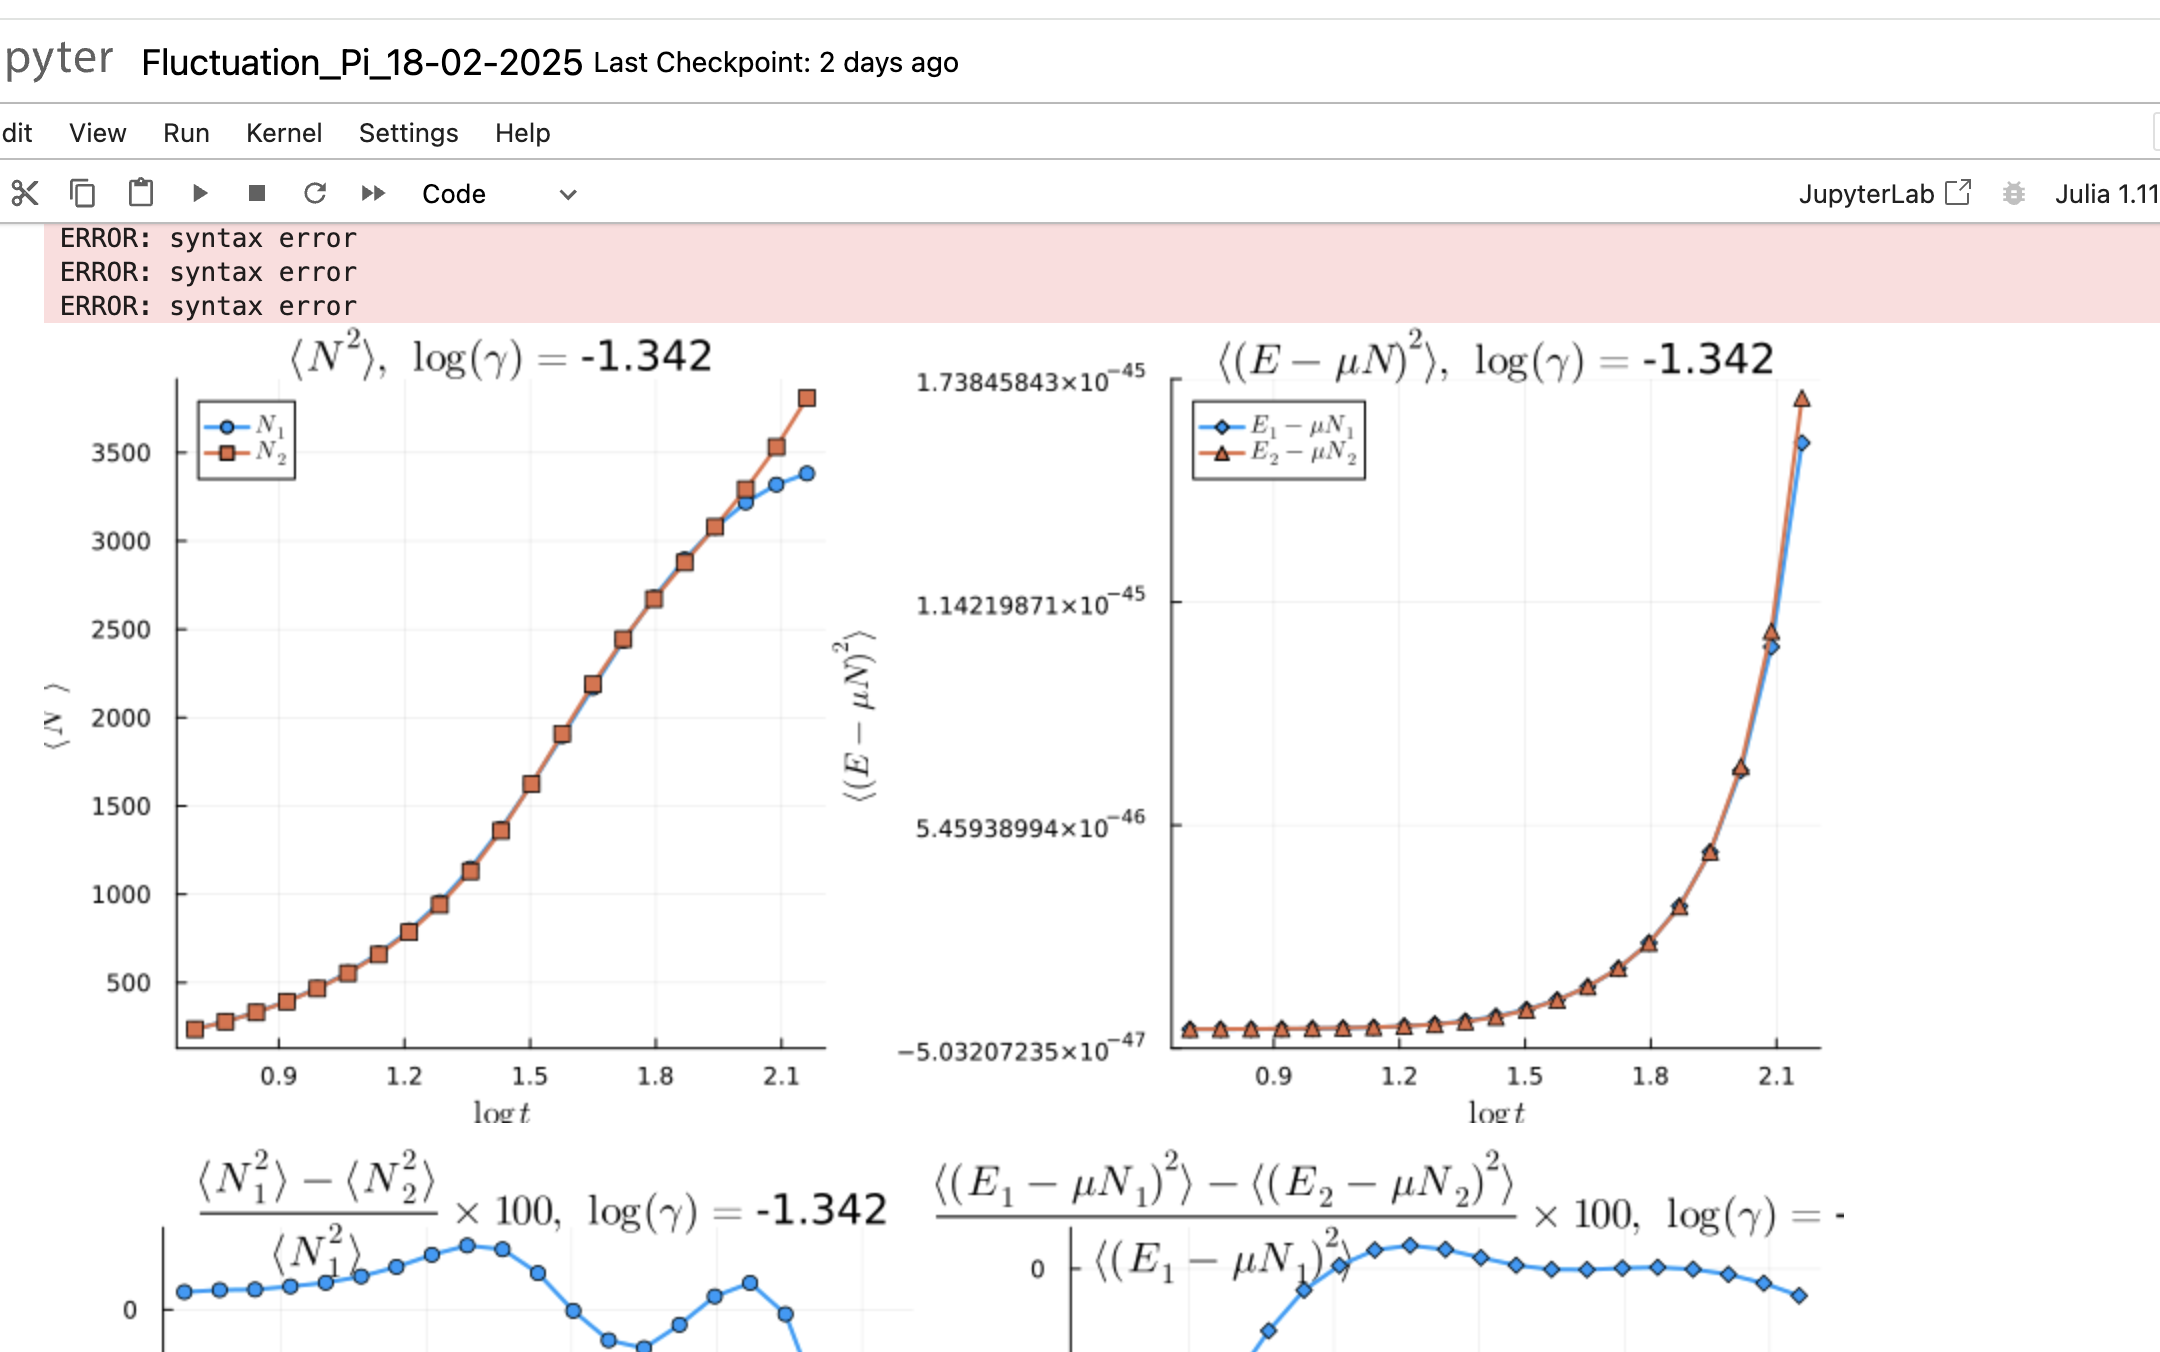
\includegraphics[width=1\textwidth]{Figures/test}

%\begin{aff}
%Donc une a l'ordre un en $\delta \theta (\operator{A}^{(0)})^{-1} %\operator{V}$ 

%\begin{eqnarray*}
%	\langle \delta \Pi ( \theta) \delta \Pi ( \theta') \rangle & = &  ( (\Pi^c_s - \Pi^c)\Pi^c/\Pi^c_s ) ( \theta ) \delta_{\theta, \theta'}/\delta \theta + \mathscr{F}(\theta , \theta' ) ,	
%\end{eqnarray*}

%avec 

%\begin{eqnarray*}
%	\mathscr{F}(\theta , \theta' ) & = & \left [ (\Pi^c_s - \Pi^c )( \theta)  +  (\Pi^c_s - \Pi^c ) ( \theta' )\right ] \frac{\Pi^c}{\Pi^c_s}(\theta)\frac{\Pi^c}{\Pi^c_s}(\theta') \frac{ \Delta( \theta'- \theta )}{ 2 \pi }\\
%	&&  - \left [ (\Pi^c_s - \Pi^c )( \theta)   (\Pi^c_s - \Pi^c ) ( \theta' )\right ] \frac{\Pi^c}{\Pi^c_s}(\theta)\frac{\Pi^c}{\Pi^c_s}(\theta')\int d\theta'' \left (   \frac{ \Pi^c/\Pi^c_s}{\Pi^c_s - \Pi^c} \right )(\theta'') \frac{\Delta(\theta''- \theta)}{2 \pi}\frac{\Delta(\theta''- \theta')}{2 \pi}  	
%\end{eqnarray*}
%\end{aff}



 









\subsection{Opérateurs conservés (intégrales du mouvement)}
%%Dans ce chapitre, nous nous intéressons aux fluctuations de la distribution de rapidité \( \delta \rho \) autour d'une distribution de référence \( \rho^c \), qui maximise la contribution à la fonction de partition des états, exprimée comme une fonctionnelle de la distribution \( \rho \) : 

La fonction de partition des états, s'exprime comme une fonctionnelle de la distribution \( \rho \) : 

\begin{eqnarray*}
	\Xi & = & \sum_\rho \exp \left( -\mathcal{A}(\rho) \right).
\end{eqnarray*}  

Dans la section {\em \bf Entropie de Yang-Yang} (\ref{??}), l'action \( \mathcal{A}(\rho) \) s'écrit sous la forme :  

\begin{eqnarray*}
	\mathcal{A}(\rho) & \doteq & - L\mathcal{S}_{YY}(\rho) + L\int f(\theta) \rho (\theta) \, d\theta,		
\end{eqnarray*}  

où \( \mathcal{S}_{YY} \) est la fonctionnelle d'entropie de Yang-Yang, définie dans (\ref{??}), et \( f \) est la fonction paramétrant les charges, introduite dans (\ref{??}).  

Dans cette même section {\em \bf Entropie de Yang-Yang} (\ref{??}), nous avons établi un lien entre \( f \) et distribution de référence \( \rho^c \), qui maximise la contribution à la fonction de partition des états .\\

On veux tester si nos experience est décrit pas un GGE. Pour cela nous nous intéressons aux fluctuations de la distribution de rapidité \( \delta \rho \) autour \( \rho^c \).

%Nous poursuivons à présent avec cette définition de l'action de classe $\mathcal{C}^2$ et admetant une distribution critique $\rho^c$ tel que sa différentielle en ce point critique soit nulle $d\mathcal{A}_{\rho^c} = 0 $ (\ref{??}) de sorte que d'aprés la formule de Taylor-Youg %afin de déterminer les fluctuations autour de \( \Pi^c \). Pour cela, nous réécrivons l'action sous la forme :  

Nous poursuivons à présent avec cette définition de l'action de classe $\mathcal{C}^2$ et admetant une distribution critique $\rho^c$ tel que sa différentielle en ce point critique soit nulle $d\mathcal{A}_{\rho^c} = 0 $ (\ref{??}) de sorte que d'aprés la formule de Taylor-Youg %afin de déterminer les fluctuations autour de \( \Pi^c \). Pour cela, nous réécrivons l'action sous la forme :  

\begin{eqnarray*}  
	\mathcal{A}(\rho^c + \delta \rho) & \underset{ \delta \rho \to 0 }{=} & \mathcal{A}(\rho^c)  + \frac{1}{2} \left. \frac{\delta^2 \mathcal{A}}{\delta \rho^2} \right|_{\rho^c} (\delta \rho) + \mathcal{O}((\delta \rho)^3),  
\end{eqnarray*}  

une expression quadratique pour l'action à l'ordre dominant en \( \delta \Pi \) avec $\left. \frac{\delta^2 \mathcal{A}}{\delta \rho^2} \right|_{\rho^c}$ la forme quadratique définie positive (Fig (\ref{fig.fluctu.A})).

\begin{figure}[H]
	\centering 
	\begin{tikzpicture}
		\begin{scope}[shift={(0,0)}]
			\begin{scope}[transform canvas={scale=0.6}]
				% Définition des couleurs avec les codes HTML
\definecolor{colorOne}{HTML}{443E46}
\definecolor{colorTwo}{HTML}{F6DEB8}
\definecolor{colorThree}{HTML}{908CA4}
\definecolor{colorFour}{HTML}{57659E}
\definecolor{colorFive}{HTML}{C57284}
\definecolor{colorSix}{HTML}{FF5B69}

% Raccourcis pour les couleurs
\def\colorOne{colorOne}
\def\colorTwo{colorTwo}
\def\colorThree{colorThree}
\def\colorFour{colorFour}
\def\colorFive{colorFive}
\def\colorSix{colorSix}

\def\colorslide{blue!50!black}



\begin{scope}
	% Tracer une courbe lisse entre des points
	\draw[shift={(0,0)} ,\colorOne]
		(-1 , 0 ) edge [thick,line width=0.8ex , ->,>=triangle 45  , \colorOne] node [pos = 1 , below ]{\huge$\rho$}( 5  , 0 )
	;
	\draw[shift={(0,0)}, color=\colorOne]
		(0, -1.0 ) edge [thick,line width=0.8ex , ->,>=triangle 45  ]node [pos=0.9,left=0.2cm ]{\huge$\mathcal{A}(\rho)$}( 0  , 5 )
	;
	\draw[]
		(2.5, 0.12 ) edge [thick,line width=0.8ex ,\colorThree ]node [pos=1,below  ]{\huge$\rho^c$} (2.5, -0.12 )	
	;
	
	\draw[]
		(2.5, -0.12 ) edge [thick,line width=0.4ex , dashed, \colorThree ] (2.5, 5.5 )
		(1.5, 1 ) edge [thick,line width=0.4ex , <->,>=triangle 45  , \colorThree ] (3.5, 1 )
		(-0.3,1) edge [thick,line width=0.4ex  , \colorThree ] node [pos=0,left ]{\huge$\mathcal{A}(\rho^c)$} (0.3, 1 )	
	;
    \draw[thick, line width=0.8ex , \colorFour] plot[smooth, tension=0.7] coordinates {
        (1, 5) (1.6 , 3 ) (2.5, 1) (3.5 , 3 )  (4, 5)
    };		
	
\end{scope}

	
			
			\end{scope}
			
			\draw[color = red , scale = 0.5 , draw = none  ] (-2 , -1) rectangle (5, 6) ; 	
		\end{scope}
		
		\begin{scope}[shift={(19,-1)}]
			\begin{scope}[transform canvas={scale=0.6}]
				% Définition des couleurs avec les codes HTML
\definecolor{colorOne}{HTML}{443E46}
\definecolor{colorTwo}{HTML}{F6DEB8}
\definecolor{colorThree}{HTML}{908CA4}
\definecolor{colorFour}{HTML}{57659E}
\definecolor{colorFive}{HTML}{C57284}
\definecolor{colorSix}{HTML}{FF5B69}

% Raccourcis pour les couleurs
\def\colorOne{colorOne}
\def\colorTwo{colorTwo}
\def\colorThree{colorThree}
\def\colorFour{colorFour}
\def\colorFive{colorFive}
\def\colorSix{colorSix}

\def\colorslide{blue!50!black}

\def\Occupation{
	\def\traitx{0.3}
	\def\traity{0.5}
	\draw[shift={(0,0)}]
		(-13.5 , 0 ) edge [thick,line width=0.8ex ]( -3.2  , 0 )
		( -3.2 - \traitx  , 0 - \traity ) edge [thick,line width=0.8ex ]( -3.2 + \traitx  , 0 + \traity  )
		( -2.8 - \traitx  , 0 - \traity ) edge [thick,line width=0.8ex ]( -2.8 + \traitx  , 0 + \traity  )
		(-2.8 , 0 ) edge [thick,line width=0.8ex ](2.8  , 0 )
		( 2.8 - \traitx  , 0 - \traity ) edge [thick,line width=0.8ex ]( 2.8 + \traitx  , 0 + \traity  )
		( 3.2 - \traitx  , 0 - \traity ) edge [thick,line width=0.8ex ]( 3.2 + \traitx  , 0 + \traity  )
		(3.2, 0 ) edge [thick,line width=0.8ex,->,>=triangle 45 , color = black ]node [pos=1.01,below  ]{\huge$\theta$}	( 13  , 0 )
	;
	\draw[shift={(0,0)}, color=\colorOne]
		(-10.5 , -1.5 ) edge [thick,line width=0.8ex , ->,>=triangle 45  ]( -10.5  , 4.5 )
	;
		
	\foreach \r in {1 , ... , 3 } {
%		\draw[
%		decoration={
%		markings,
%    	mark connection node=my node,
%    	mark=at position 0 with{\node [blue,transform shape] (my node) {\large \r};}},
%		color=gray, thick, 
%		line width=0.5ex] decorate { 
%            (-11.0, \r) -- (-10.1, \r )}
%        ;
        \draw[
			color=\colorOne,
			] 
            (-11.0, \r) edge[color=\colorThree , thick,line width=0.5ex] node [pos=-0.5 ]{\large\color{\colorFour} $\frac{\r}{\delta \theta}$ } (-10.3, \r )
        	;
	
	}
	

	
	% Graduation abcsisse 
	% Définitions des listes
% Definitions of the lists
\def\listetuple{-9/\theta_{1}, -8/\theta_{2} , -5/\theta_{3} , -2/\theta_{a-1} , 0/\theta_{a} , 1/\theta_{a+1} , 2/\theta_{a+2} ,  5/\theta_{N-4} , 7/\theta_{N-3},8/\theta_{N-1},9/\theta_{N} }
\def\listetrais{-12 , -11, -10, -9 , -8 , -7 ,  -6 , -5, -4.5,-4, -2 , -1, 0 , 0.5, 1, 2, 4 , 5 ,  6 , 7 , 8 ,8.5, 9 ,  10 , 11, 12 }

% Loop over listetrais
\foreach \r in \listetrais {
    % Initialize found variable to zero
    % Initialize found variable to zero
    %\pgfmathsetmacro\found{0}
    \global\def\found{0}
    \xdef\nomtheta{}
    
    % Check if \r is in listetuple
    \foreach \x/\y in \listetuple { 
        \ifdim \r pt=\x pt % If \r matches any \x in listetuple
            \global\def\found{1} ;
            \xdef\nomtheta{\y} % Set \nomtheta to the corresponding \y
            %\pgfmathsetmacro\found{1} % Set found to 1            
            %\global\pgfmathsetmacro\found{1}
        \fi
    }
    
    %\node [circle, draw, red] (A) at (\r, 2) {\found , $\nomtheta$};
    
    % Draw the line and display \nomtheta if found
    \ifnum\found=1
        \draw[color=\colorOne, thick, line width=0.5ex] 
            (\r, -0.3) -- (\r, 0.3) node[red , pos=-0.5] {\large $\nomtheta$};
         \filldraw[line width=0.5ex, color=\colorSix, outer color=\colorSix, inner color=\colorSix] 
            (\r, 0) circle (4pt);
    \else 
        % Draw without \nomtheta and add a blue circle if not found
        \draw[color=\colorOne, thick, line width=0.5ex] 
            (\r, -0.3) -- (\r, 0.3);
        \filldraw[line width=0.5ex, color=\colorSix, outer color=\colorTwo, inner color=\colorTwo] 
            (\r, 0) circle (4pt); 
    \fi
}

\def\listetrais{-9.5/\theta_{i-1}/2/3, -6.5/\theta_{i}/1/4  ,   -1.5/\theta_{j}/2/4 , 1.5/\theta_{j+1}/-1/3 , 3.5/\theta_{\ell-1}/1/3 , 6.5/\theta_{\ell}/3/4 , 9.5/\theta(\theta_{\ell+1})/-1/3 };



\foreach \r/\nomx/\y/\ys in \listetrais {
	\draw[
		decoration={
		markings,
    	mark connection node=my node,
    	mark=at position .5 with{\node [blue,transform shape] (my node) {\large \color{\colorFour} $\nomx$};}},
		color=\colorThree , thick, 
		line width=0.5ex] decorate { 
            (\r, 0.12) -- (\r, -1.2)}
        ;
     
     \ifdim \y pt > -1 pt 
     	\draw[
			decoration={
			markings,
    		mark connection node=my node,
    		mark=at position .5 with{\node [blue,transform shape] (my node) {\large \color{\colorFour} $\Pi(\nomx) $};}},
			color=\colorThree, thick, 
			line width=0.5ex] decorate { 
            (\r, \y) -- (\r +3, \y)}
        ;
        \draw[
			decoration={
			markings,
    		mark connection node=my node,
    		mark=at position .5 with{\node [blue,transform shape] (my node) {\large \color{\colorFive} $\Pi_s(\nomx) $};}},
			color=\colorFive, thick, 
			line width=0.5ex] decorate { 
            (\r, \ys) -- (\r +3, \ys)}
        ;
     \fi 
     \ifdim \r pt= -1.5 pt
     	\draw[
     		decoration={
			markings,
    		mark connection node=my node,
    		mark=at position .5 with{\node [blue,transform shape] (my node) {\large \color{\colorFour}  $\delta \theta $};},
    		%mark=at position 0.1  with {\arrow[blue, line width=0.5ex]{<}},
    		%mark=at position 1  with {\arrow[blue, line width=0.5ex]{>}}
    		},
        	color=\colorThree,
        	thick,
        	line width=0.5ex,
        	%arrows={Computer Modern Rightarrow[line cap=round]-Computer Modern Rightarrow[line cap=round]}
   			](\r, -1.2) edge[arrows={Computer Modern Rightarrow[line cap=round]-}] (\r + 0.4, -1.2)decorate {
    		(\r, -1.2) -- (\r + 3, -1.2)}(\r + 2, -1.2) edge[arrows={-Computer Modern Rightarrow[line cap=round]}] (\r + 3, -1.2)
    		;
    \fi
			
	
}


			
}


\begin{scope}
	%\draw[help lines , width=1.5ex] (-8,-3) grid (8,3);\draw[help lines ,width=0.5ex , opacity = 0.5] (-3,-3) grid[step=0.1] (3,3));
	
	%\draw[help lines] 
	%	(-3,-3) edge[width=1.5ex] grid (3,3)	
	%	(-3,-3) edge[width=0.5ex , opacity = 0.5] grid (3,3)	
	%;
	\begin{scope}[shift={(0,1)},rotate=0,opacity=1,color=black]
		\Occupation	
		
		%\node[anchor=east, font=\bfseries] at (-11, 0) {\color{red}\large (T = 0 )} ;	
	\end{scope}
	
	
	
	
	\begin{scope}[shift={(-10.5,7)},rotate=0,opacity=1,color=black]
	
	\begin{scope}[shift={(-0,0)},rotate=0,opacity=1,color=black]
	
		\draw[shift={(0,0)} ,line width=1ex,rounded corners = 1ex,color=\colorOne , opacity =1 ,fill=\colorOne!00 , pattern={north east lines} , pattern color=\colorOne!00 ]
			(0 , -1 ) rectangle (5,1)
		;
		

		\begin{scope}[shift={(0.5,0.5)}]
			\draw[color=\colorOne, thick, line width=0.5ex] 
            (0, -0.3) -- (0, 0.3) ;
            \filldraw[line width=0.5ex, color=\colorSix, outer color=\colorSix, inner color=\colorSix] 
            (0, 0) circle (4pt);
            
            \node[anchor=west, font=\bfseries] at (0.2, 0) {\color{\colorSix}\large : quasi-particule};
		\end{scope}
		
		\begin{scope}[shift={(0.5,-0.5)}]
			\draw[color=\colorOne, thick, line width=0.5ex] 
            (0, -0.3) -- (0, 0.3) ;
            \filldraw[line width=0.5ex, color=\colorSix, outer color=\colorTwo, inner color=\colorTwo] 
            (0, 0) circle (4pt);
            
            \node[anchor=west, font=\bfseries] at (0.2, 0) {\color{\colorSix}\large : hole};
		\end{scope}

	\end{scope}
	
	\begin{scope}[shift={(6,0)},rotate=0,opacity=1,color=black]	
		
		\draw[shift={(0,0)} ,line width=1ex,rounded corners = 1ex,color=\colorOne , opacity =1 ,fill=\colorOne!00 , pattern={north east lines} , pattern color=\colorOne!00 ]
			(0 , -1 ) rectangle (7.5,1)
		;
		
		\node[anchor=west] at (0.5, 0.5) {\color{\colorFour}\large $\Pi$ };\node[anchor=west, font=\bfseries] at (1, 0.5) {\color{\colorFour}\large : quasi-particule distribution};
		
		\node[anchor=west] at (0.5, -0.5) {\color{\colorFour}\large $\Pi_h$ };\node[anchor=west, font=\bfseries] at (1, -0.5) {\color{\colorFour}\large  : hole distribution};
		
	\end{scope}
	
	\begin{scope}[shift={(14.5,0)},rotate=0,opacity=1,color=black]	
		
		\draw[shift={(0,0)} ,line width=1ex,rounded corners = 1ex,color=\colorOne , opacity =1 ,fill=\colorOne!00 , pattern={north east lines} , pattern color=\colorOne!00 ]
			(0 , -0.5 ) rectangle (7.0,0.5)
		;
		
		\node[anchor=west] at (0.2, 0) {\color{\colorFour}\large ${\color{\colorFive}\Pi_s} = \Pi + \Pi_h $ } node[anchor=west , font=\bfseries] at (3.1 , 0 )  {\color{\colorFour}\large {\color{\colorFive} : density of states}};
		
	\end{scope}
	
	
	\end{scope}


		
	
\end{scope}

	
			
			\end{scope}
			\begin{scope}[scale=1]
				\draw[color = red , scale = 1 , draw = none  ] (-1 , -1) rectangle (5, 5) ; 
			\end{scope}	
		\end{scope}

		
				
			
	\end{tikzpicture}	
	\captionsetup{skip=10pt} % Ajoute de l’espace après la légende
	\label{fig.fluctu.A}
\end{figure}


On discrétise l'axe des rapidités en  petite cellule de rapidité $[\theta, \theta+\delta\theta]$, qui contient $L\rho(\theta) \delta \theta$ rapidités. 
	



Avec ces petites tranches, la forme quadratique s’écrit :

\begin{eqnarray*}
    \left. \frac{\delta^2 \mathcal{A}}{{\delta \rho}^2} \right|_{\rho^c}(\delta \rho ) &=&  \sum_{a,b \mid \text{tranche}}  
    \delta \rho(\theta_a)  \frac{\partial^2 \mathcal{A}}{\partial \delta \rho(\theta_a) \partial \delta \rho(\theta_b) } (\rho^c)  \delta \rho(\theta_b).
\end{eqnarray*}
Les fluctuations s’écrivent donc :

\begin{eqnarray*}
    \langle \delta \rho ( \theta) \delta \rho ( \theta') \rangle &=&  
    \frac{ \int d\delta \rho \, \delta \rho(\theta) \delta \rho ( \theta') 
    \exp \left( - \frac{1}{2} \sum_{a,b \mid \text{tranche}}  
    \delta \rho(\theta_a) \frac{\partial^2 \mathcal{A}}{\partial \delta \rho(\theta_a) \partial \delta \rho(\theta_b) } (\rho^c)  \delta \rho(\theta_b) \right) }
    { \int d\delta \Pi  
    \exp \left( - \frac{1}{2} \sum_{a,b \mid \text{tranche}}  
    \delta \rho(\theta_a) \frac{\partial^2 \mathcal{A}}{\partial \delta \rho(\theta_a) \partial \delta \rho(\theta_b) } (\rho^c)  \delta \rho(\theta_b) \right) } \\
    &=& \left( \mathbf{A}^{-1} \right)_{\theta , \theta'}
\end{eqnarray*}


\begin{aff}

\begin{eqnarray*}
	\langle \delta \rho ( \theta) \delta \rho ( \theta') \rangle &=& 	\left( \mathbf{A}^{-1} \right)_{\theta , \theta'}
\end{eqnarray*}

	
avec la  {\em matrice hessienne} $\mathbf{A}_{\theta , \theta'} \equiv \frac{\partial^2 \mathcal{A}}{\partial \delta \rho(\theta) \partial \delta \rho(\theta') }(\rho^c)$, au point critique/ qui maximise la probabilité  $\rho^c=\rho^c_s \nu^c $, s'écrit

\begin{eqnarray*}
	\operator{A} & = & \operator{A}^{(0)} + \delta \theta \operator{V}
\end{eqnarray*}

avec 

\begin{eqnarray*}
	A^{(0)}_{\theta , \theta'}  & = &  L\delta \theta \left ( \frac{ 1}{\rho^c_s ( 1  - \nu^c ) \nu^c } \right )(\theta)    \delta({\theta - \theta '})	,\\
	V_{\theta , \theta'}  &= & L \delta \theta \left \{ - \left [ \left ( \frac{1}{\rho^c_s( 1 - \nu^c) } \right ) ( \theta)  +  \left ( \frac{1}{\rho^c_s( 1 - \nu^c) } \right ) ( \theta' )\right ] \frac{ \Delta( \theta'- \theta )}{ 2 \pi } + \int d\theta''  \left ( \frac{\nu^c}{\rho^c_s( 1 - \nu^c) } \right )(\theta'') \frac{\Delta(\theta''- \theta)}{2 \pi}\frac{\Delta(\theta''- \theta')}{2 \pi}   \right \} 	
\end{eqnarray*}

\end{aff}

\subsection{Testes}

\begin{eqnarray*}
	\Delta_{\operator{\mathcal{N}}}^2  & = &  \frac{1}{\beta} \left . \frac{\partial \langle \operator{\mathcal{N}} \rangle}{\partial \mu} \right )_T \\
	\Delta_{\operator{\mathcal{E}}-\mu \operator{\mathcal{N}}}^2  & = &  - \left . \frac{\partial \langle \operator{\mathcal{E}}-\mu \operator{\mathcal{N}} \rangle}{\partial \beta} \right )_\mu 
\end{eqnarray*}

et 

\begin{eqnarray*}
	\Delta_{\operator{\mathcal{N}}}^2  &= & L^2 \int d\theta_a \int d \theta_b \, \langle \delta \rho(\theta_a) \delta \rho(\theta_b) \rangle \\
	\Delta_{\operator{\mathcal{E}}-\mu \operator{\mathcal{N}}}^2  & = & L^2 \int d\theta_a \int d \theta_b \, \left ( - \mu + \frac{1}2 m \theta_a^2  \right  )\left ( - \mu + \frac{1}2 m \theta_b^2  \right  )  \langle \delta \rho(\theta_a) \delta \rho(\theta_b) \rangle
\end{eqnarray*}

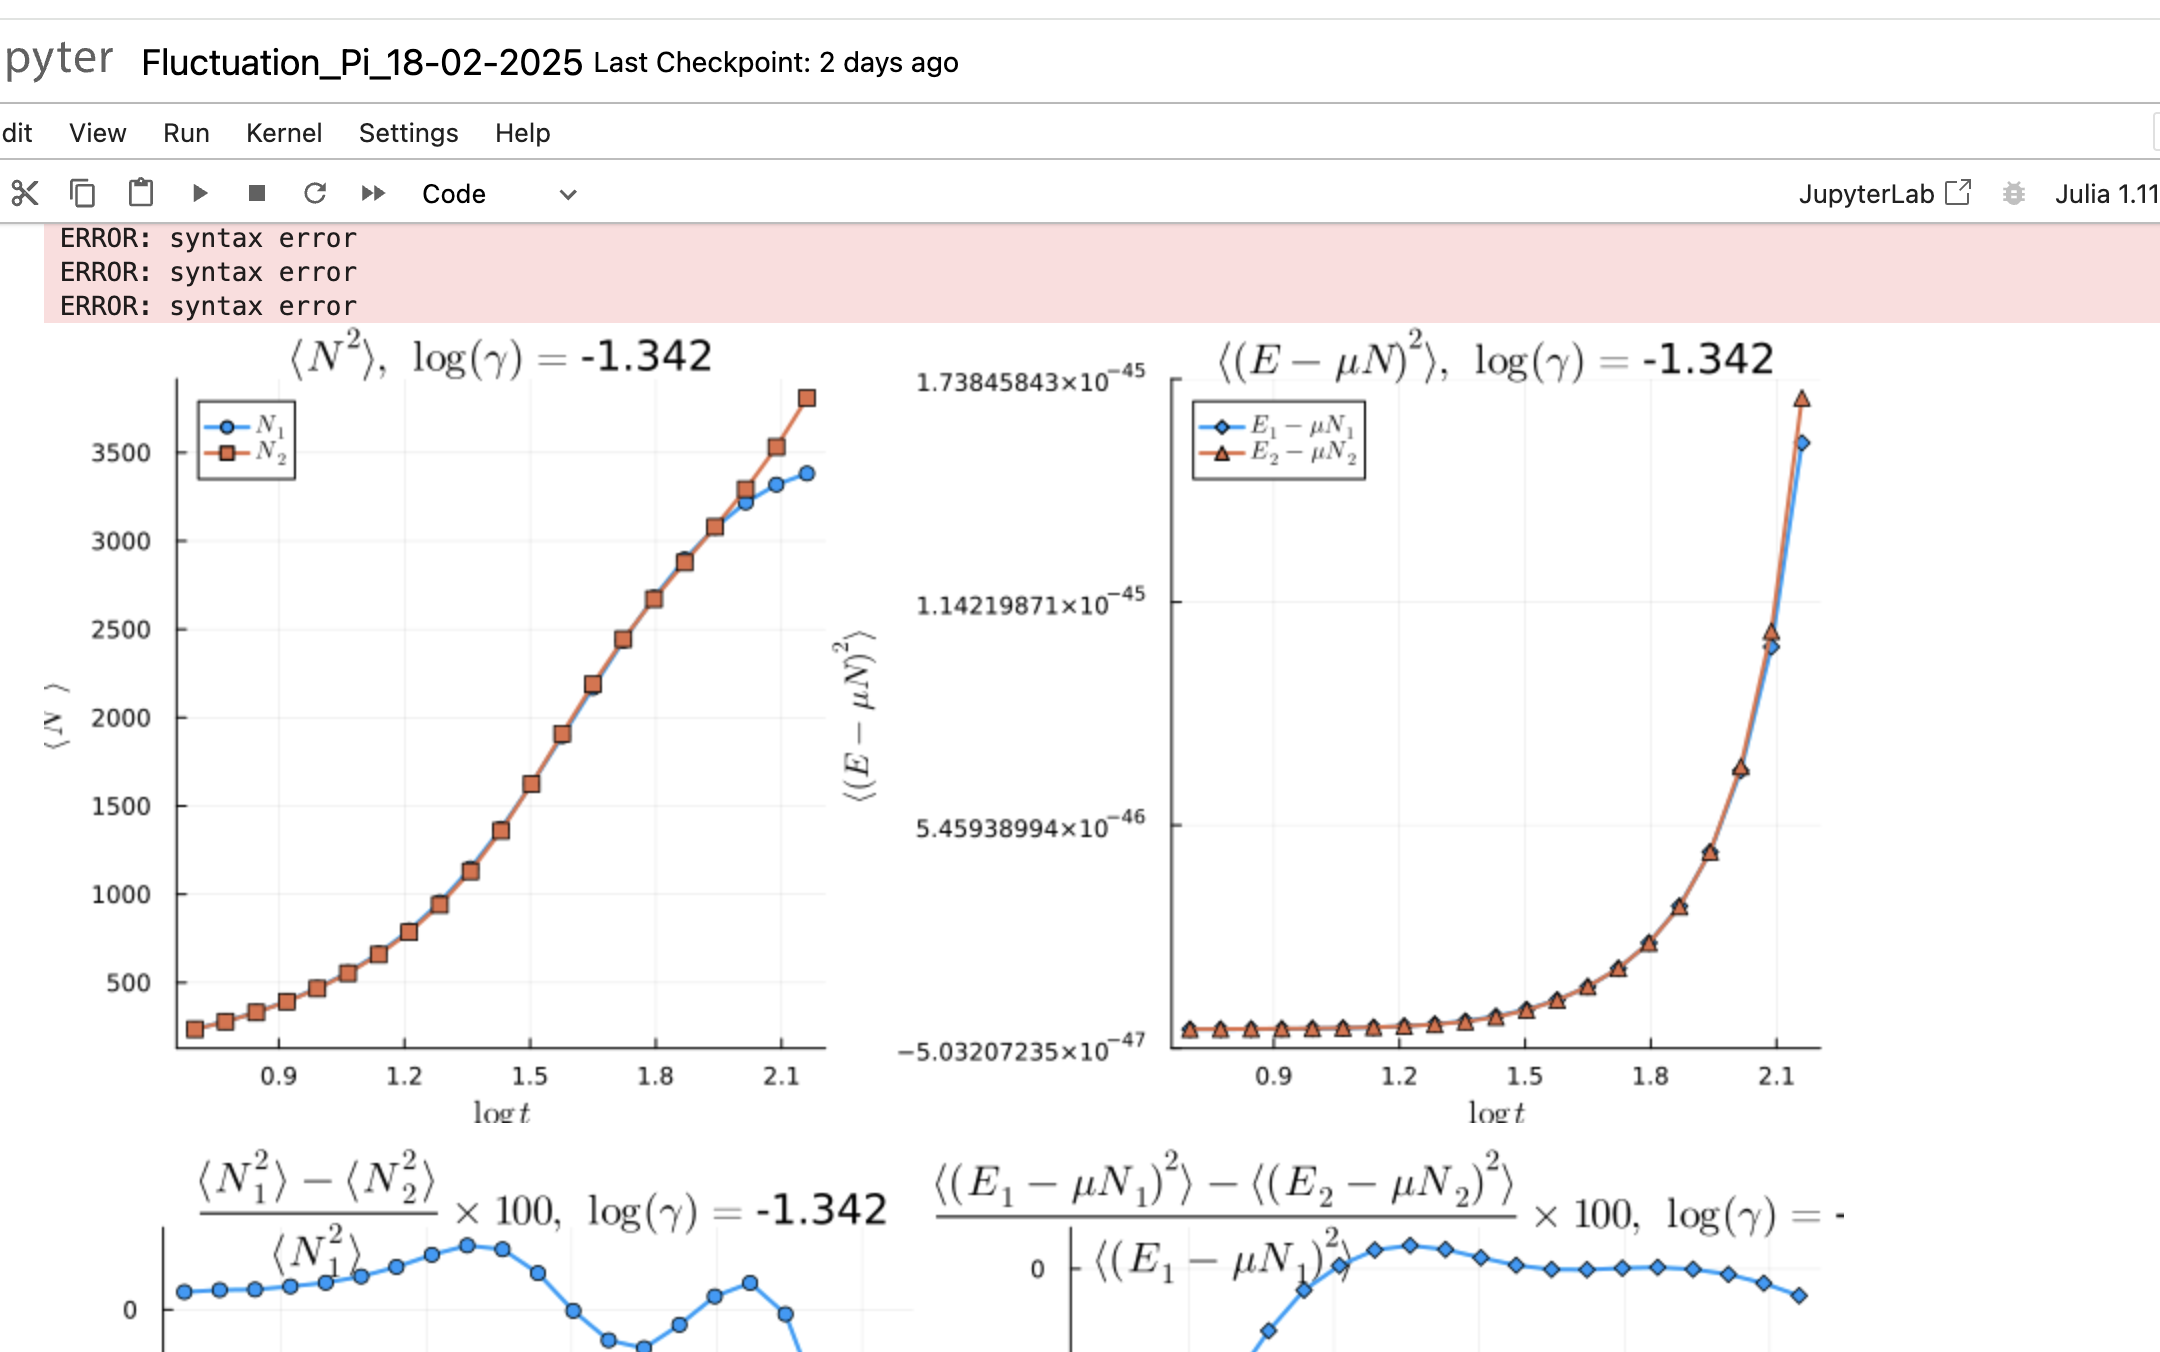
\includegraphics[width=1\textwidth]{Figures/test}

%\begin{aff}
%Donc une a l'ordre un en $\delta \theta (\operator{A}^{(0)})^{-1} %\operator{V}$ 

%\begin{eqnarray*}
%	\langle \delta \Pi ( \theta) \delta \Pi ( \theta') \rangle & = &  ( (\Pi^c_s - \Pi^c)\Pi^c/\Pi^c_s ) ( \theta ) \delta_{\theta, \theta'}/\delta \theta + \mathscr{F}(\theta , \theta' ) ,	
%\end{eqnarray*}

%avec 

%\begin{eqnarray*}
%	\mathscr{F}(\theta , \theta' ) & = & \left [ (\Pi^c_s - \Pi^c )( \theta)  +  (\Pi^c_s - \Pi^c ) ( \theta' )\right ] \frac{\Pi^c}{\Pi^c_s}(\theta)\frac{\Pi^c}{\Pi^c_s}(\theta') \frac{ \Delta( \theta'- \theta )}{ 2 \pi }\\
%	&&  - \left [ (\Pi^c_s - \Pi^c )( \theta)   (\Pi^c_s - \Pi^c ) ( \theta' )\right ] \frac{\Pi^c}{\Pi^c_s}(\theta)\frac{\Pi^c}{\Pi^c_s}(\theta')\int d\theta'' \left (   \frac{ \Pi^c/\Pi^c_s}{\Pi^c_s - \Pi^c} \right )(\theta'') \frac{\Delta(\theta''- \theta)}{2 \pi}\frac{\Delta(\theta''- \theta')}{2 \pi}  	
%\end{eqnarray*}
%\end{aff}



 








%\subsection{Introduction au modèle de gaz de Bose unidimensionnel}
%Dans ce chapitre, nous nous intéressons aux fluctuations de la distribution de rapidité \( \delta \rho \) autour d'une distribution de référence \( \rho^c \), qui maximise la contribution à la fonction de partition des états, exprimée comme une fonctionnelle de la distribution \( \rho \) : 

La fonction de partition des états, s'exprime comme une fonctionnelle de la distribution \( \rho \) : 

\begin{eqnarray*}
	\Xi & = & \sum_\rho \exp \left( -\mathcal{A}(\rho) \right).
\end{eqnarray*}  

Dans la section {\em \bf Entropie de Yang-Yang} (\ref{??}), l'action \( \mathcal{A}(\rho) \) s'écrit sous la forme :  

\begin{eqnarray*}
	\mathcal{A}(\rho) & \doteq & - L\mathcal{S}_{YY}(\rho) + L\int f(\theta) \rho (\theta) \, d\theta,		
\end{eqnarray*}  

où \( \mathcal{S}_{YY} \) est la fonctionnelle d'entropie de Yang-Yang, définie dans (\ref{??}), et \( f \) est la fonction paramétrant les charges, introduite dans (\ref{??}).  

Dans cette même section {\em \bf Entropie de Yang-Yang} (\ref{??}), nous avons établi un lien entre \( f \) et distribution de référence \( \rho^c \), qui maximise la contribution à la fonction de partition des états .\\

On veux tester si nos experience est décrit pas un GGE. Pour cela nous nous intéressons aux fluctuations de la distribution de rapidité \( \delta \rho \) autour \( \rho^c \).

%Nous poursuivons à présent avec cette définition de l'action de classe $\mathcal{C}^2$ et admetant une distribution critique $\rho^c$ tel que sa différentielle en ce point critique soit nulle $d\mathcal{A}_{\rho^c} = 0 $ (\ref{??}) de sorte que d'aprés la formule de Taylor-Youg %afin de déterminer les fluctuations autour de \( \Pi^c \). Pour cela, nous réécrivons l'action sous la forme :  

Nous poursuivons à présent avec cette définition de l'action de classe $\mathcal{C}^2$ et admetant une distribution critique $\rho^c$ tel que sa différentielle en ce point critique soit nulle $d\mathcal{A}_{\rho^c} = 0 $ (\ref{??}) de sorte que d'aprés la formule de Taylor-Youg %afin de déterminer les fluctuations autour de \( \Pi^c \). Pour cela, nous réécrivons l'action sous la forme :  

\begin{eqnarray*}  
	\mathcal{A}(\rho^c + \delta \rho) & \underset{ \delta \rho \to 0 }{=} & \mathcal{A}(\rho^c)  + \frac{1}{2} \left. \frac{\delta^2 \mathcal{A}}{\delta \rho^2} \right|_{\rho^c} (\delta \rho) + \mathcal{O}((\delta \rho)^3),  
\end{eqnarray*}  

une expression quadratique pour l'action à l'ordre dominant en \( \delta \Pi \) avec $\left. \frac{\delta^2 \mathcal{A}}{\delta \rho^2} \right|_{\rho^c}$ la forme quadratique définie positive (Fig (\ref{fig.fluctu.A})).

\begin{figure}[H]
	\centering 
	\begin{tikzpicture}
		\begin{scope}[shift={(0,0)}]
			\begin{scope}[transform canvas={scale=0.6}]
				% Définition des couleurs avec les codes HTML
\definecolor{colorOne}{HTML}{443E46}
\definecolor{colorTwo}{HTML}{F6DEB8}
\definecolor{colorThree}{HTML}{908CA4}
\definecolor{colorFour}{HTML}{57659E}
\definecolor{colorFive}{HTML}{C57284}
\definecolor{colorSix}{HTML}{FF5B69}

% Raccourcis pour les couleurs
\def\colorOne{colorOne}
\def\colorTwo{colorTwo}
\def\colorThree{colorThree}
\def\colorFour{colorFour}
\def\colorFive{colorFive}
\def\colorSix{colorSix}

\def\colorslide{blue!50!black}



\begin{scope}
	% Tracer une courbe lisse entre des points
	\draw[shift={(0,0)} ,\colorOne]
		(-1 , 0 ) edge [thick,line width=0.8ex , ->,>=triangle 45  , \colorOne] node [pos = 1 , below ]{\huge$\rho$}( 5  , 0 )
	;
	\draw[shift={(0,0)}, color=\colorOne]
		(0, -1.0 ) edge [thick,line width=0.8ex , ->,>=triangle 45  ]node [pos=0.9,left=0.2cm ]{\huge$\mathcal{A}(\rho)$}( 0  , 5 )
	;
	\draw[]
		(2.5, 0.12 ) edge [thick,line width=0.8ex ,\colorThree ]node [pos=1,below  ]{\huge$\rho^c$} (2.5, -0.12 )	
	;
	
	\draw[]
		(2.5, -0.12 ) edge [thick,line width=0.4ex , dashed, \colorThree ] (2.5, 5.5 )
		(1.5, 1 ) edge [thick,line width=0.4ex , <->,>=triangle 45  , \colorThree ] (3.5, 1 )
		(-0.3,1) edge [thick,line width=0.4ex  , \colorThree ] node [pos=0,left ]{\huge$\mathcal{A}(\rho^c)$} (0.3, 1 )	
	;
    \draw[thick, line width=0.8ex , \colorFour] plot[smooth, tension=0.7] coordinates {
        (1, 5) (1.6 , 3 ) (2.5, 1) (3.5 , 3 )  (4, 5)
    };		
	
\end{scope}

	
			
			\end{scope}
			
			\draw[color = red , scale = 0.5 , draw = none  ] (-2 , -1) rectangle (5, 6) ; 	
		\end{scope}
		
		\begin{scope}[shift={(19,-1)}]
			\begin{scope}[transform canvas={scale=0.6}]
				% Définition des couleurs avec les codes HTML
\definecolor{colorOne}{HTML}{443E46}
\definecolor{colorTwo}{HTML}{F6DEB8}
\definecolor{colorThree}{HTML}{908CA4}
\definecolor{colorFour}{HTML}{57659E}
\definecolor{colorFive}{HTML}{C57284}
\definecolor{colorSix}{HTML}{FF5B69}

% Raccourcis pour les couleurs
\def\colorOne{colorOne}
\def\colorTwo{colorTwo}
\def\colorThree{colorThree}
\def\colorFour{colorFour}
\def\colorFive{colorFive}
\def\colorSix{colorSix}

\def\colorslide{blue!50!black}

\def\Occupation{
	\def\traitx{0.3}
	\def\traity{0.5}
	\draw[shift={(0,0)}]
		(-13.5 , 0 ) edge [thick,line width=0.8ex ]( -3.2  , 0 )
		( -3.2 - \traitx  , 0 - \traity ) edge [thick,line width=0.8ex ]( -3.2 + \traitx  , 0 + \traity  )
		( -2.8 - \traitx  , 0 - \traity ) edge [thick,line width=0.8ex ]( -2.8 + \traitx  , 0 + \traity  )
		(-2.8 , 0 ) edge [thick,line width=0.8ex ](2.8  , 0 )
		( 2.8 - \traitx  , 0 - \traity ) edge [thick,line width=0.8ex ]( 2.8 + \traitx  , 0 + \traity  )
		( 3.2 - \traitx  , 0 - \traity ) edge [thick,line width=0.8ex ]( 3.2 + \traitx  , 0 + \traity  )
		(3.2, 0 ) edge [thick,line width=0.8ex,->,>=triangle 45 , color = black ]node [pos=1.01,below  ]{\huge$\theta$}	( 13  , 0 )
	;
	\draw[shift={(0,0)}, color=\colorOne]
		(-10.5 , -1.5 ) edge [thick,line width=0.8ex , ->,>=triangle 45  ]( -10.5  , 4.5 )
	;
		
	\foreach \r in {1 , ... , 3 } {
%		\draw[
%		decoration={
%		markings,
%    	mark connection node=my node,
%    	mark=at position 0 with{\node [blue,transform shape] (my node) {\large \r};}},
%		color=gray, thick, 
%		line width=0.5ex] decorate { 
%            (-11.0, \r) -- (-10.1, \r )}
%        ;
        \draw[
			color=\colorOne,
			] 
            (-11.0, \r) edge[color=\colorThree , thick,line width=0.5ex] node [pos=-0.5 ]{\large\color{\colorFour} $\frac{\r}{\delta \theta}$ } (-10.3, \r )
        	;
	
	}
	

	
	% Graduation abcsisse 
	% Définitions des listes
% Definitions of the lists
\def\listetuple{-9/\theta_{1}, -8/\theta_{2} , -5/\theta_{3} , -2/\theta_{a-1} , 0/\theta_{a} , 1/\theta_{a+1} , 2/\theta_{a+2} ,  5/\theta_{N-4} , 7/\theta_{N-3},8/\theta_{N-1},9/\theta_{N} }
\def\listetrais{-12 , -11, -10, -9 , -8 , -7 ,  -6 , -5, -4.5,-4, -2 , -1, 0 , 0.5, 1, 2, 4 , 5 ,  6 , 7 , 8 ,8.5, 9 ,  10 , 11, 12 }

% Loop over listetrais
\foreach \r in \listetrais {
    % Initialize found variable to zero
    % Initialize found variable to zero
    %\pgfmathsetmacro\found{0}
    \global\def\found{0}
    \xdef\nomtheta{}
    
    % Check if \r is in listetuple
    \foreach \x/\y in \listetuple { 
        \ifdim \r pt=\x pt % If \r matches any \x in listetuple
            \global\def\found{1} ;
            \xdef\nomtheta{\y} % Set \nomtheta to the corresponding \y
            %\pgfmathsetmacro\found{1} % Set found to 1            
            %\global\pgfmathsetmacro\found{1}
        \fi
    }
    
    %\node [circle, draw, red] (A) at (\r, 2) {\found , $\nomtheta$};
    
    % Draw the line and display \nomtheta if found
    \ifnum\found=1
        \draw[color=\colorOne, thick, line width=0.5ex] 
            (\r, -0.3) -- (\r, 0.3) node[red , pos=-0.5] {\large $\nomtheta$};
         \filldraw[line width=0.5ex, color=\colorSix, outer color=\colorSix, inner color=\colorSix] 
            (\r, 0) circle (4pt);
    \else 
        % Draw without \nomtheta and add a blue circle if not found
        \draw[color=\colorOne, thick, line width=0.5ex] 
            (\r, -0.3) -- (\r, 0.3);
        \filldraw[line width=0.5ex, color=\colorSix, outer color=\colorTwo, inner color=\colorTwo] 
            (\r, 0) circle (4pt); 
    \fi
}

\def\listetrais{-9.5/\theta_{i-1}/2/3, -6.5/\theta_{i}/1/4  ,   -1.5/\theta_{j}/2/4 , 1.5/\theta_{j+1}/-1/3 , 3.5/\theta_{\ell-1}/1/3 , 6.5/\theta_{\ell}/3/4 , 9.5/\theta(\theta_{\ell+1})/-1/3 };



\foreach \r/\nomx/\y/\ys in \listetrais {
	\draw[
		decoration={
		markings,
    	mark connection node=my node,
    	mark=at position .5 with{\node [blue,transform shape] (my node) {\large \color{\colorFour} $\nomx$};}},
		color=\colorThree , thick, 
		line width=0.5ex] decorate { 
            (\r, 0.12) -- (\r, -1.2)}
        ;
     
     \ifdim \y pt > -1 pt 
     	\draw[
			decoration={
			markings,
    		mark connection node=my node,
    		mark=at position .5 with{\node [blue,transform shape] (my node) {\large \color{\colorFour} $\Pi(\nomx) $};}},
			color=\colorThree, thick, 
			line width=0.5ex] decorate { 
            (\r, \y) -- (\r +3, \y)}
        ;
        \draw[
			decoration={
			markings,
    		mark connection node=my node,
    		mark=at position .5 with{\node [blue,transform shape] (my node) {\large \color{\colorFive} $\Pi_s(\nomx) $};}},
			color=\colorFive, thick, 
			line width=0.5ex] decorate { 
            (\r, \ys) -- (\r +3, \ys)}
        ;
     \fi 
     \ifdim \r pt= -1.5 pt
     	\draw[
     		decoration={
			markings,
    		mark connection node=my node,
    		mark=at position .5 with{\node [blue,transform shape] (my node) {\large \color{\colorFour}  $\delta \theta $};},
    		%mark=at position 0.1  with {\arrow[blue, line width=0.5ex]{<}},
    		%mark=at position 1  with {\arrow[blue, line width=0.5ex]{>}}
    		},
        	color=\colorThree,
        	thick,
        	line width=0.5ex,
        	%arrows={Computer Modern Rightarrow[line cap=round]-Computer Modern Rightarrow[line cap=round]}
   			](\r, -1.2) edge[arrows={Computer Modern Rightarrow[line cap=round]-}] (\r + 0.4, -1.2)decorate {
    		(\r, -1.2) -- (\r + 3, -1.2)}(\r + 2, -1.2) edge[arrows={-Computer Modern Rightarrow[line cap=round]}] (\r + 3, -1.2)
    		;
    \fi
			
	
}


			
}


\begin{scope}
	%\draw[help lines , width=1.5ex] (-8,-3) grid (8,3);\draw[help lines ,width=0.5ex , opacity = 0.5] (-3,-3) grid[step=0.1] (3,3));
	
	%\draw[help lines] 
	%	(-3,-3) edge[width=1.5ex] grid (3,3)	
	%	(-3,-3) edge[width=0.5ex , opacity = 0.5] grid (3,3)	
	%;
	\begin{scope}[shift={(0,1)},rotate=0,opacity=1,color=black]
		\Occupation	
		
		%\node[anchor=east, font=\bfseries] at (-11, 0) {\color{red}\large (T = 0 )} ;	
	\end{scope}
	
	
	
	
	\begin{scope}[shift={(-10.5,7)},rotate=0,opacity=1,color=black]
	
	\begin{scope}[shift={(-0,0)},rotate=0,opacity=1,color=black]
	
		\draw[shift={(0,0)} ,line width=1ex,rounded corners = 1ex,color=\colorOne , opacity =1 ,fill=\colorOne!00 , pattern={north east lines} , pattern color=\colorOne!00 ]
			(0 , -1 ) rectangle (5,1)
		;
		

		\begin{scope}[shift={(0.5,0.5)}]
			\draw[color=\colorOne, thick, line width=0.5ex] 
            (0, -0.3) -- (0, 0.3) ;
            \filldraw[line width=0.5ex, color=\colorSix, outer color=\colorSix, inner color=\colorSix] 
            (0, 0) circle (4pt);
            
            \node[anchor=west, font=\bfseries] at (0.2, 0) {\color{\colorSix}\large : quasi-particule};
		\end{scope}
		
		\begin{scope}[shift={(0.5,-0.5)}]
			\draw[color=\colorOne, thick, line width=0.5ex] 
            (0, -0.3) -- (0, 0.3) ;
            \filldraw[line width=0.5ex, color=\colorSix, outer color=\colorTwo, inner color=\colorTwo] 
            (0, 0) circle (4pt);
            
            \node[anchor=west, font=\bfseries] at (0.2, 0) {\color{\colorSix}\large : hole};
		\end{scope}

	\end{scope}
	
	\begin{scope}[shift={(6,0)},rotate=0,opacity=1,color=black]	
		
		\draw[shift={(0,0)} ,line width=1ex,rounded corners = 1ex,color=\colorOne , opacity =1 ,fill=\colorOne!00 , pattern={north east lines} , pattern color=\colorOne!00 ]
			(0 , -1 ) rectangle (7.5,1)
		;
		
		\node[anchor=west] at (0.5, 0.5) {\color{\colorFour}\large $\Pi$ };\node[anchor=west, font=\bfseries] at (1, 0.5) {\color{\colorFour}\large : quasi-particule distribution};
		
		\node[anchor=west] at (0.5, -0.5) {\color{\colorFour}\large $\Pi_h$ };\node[anchor=west, font=\bfseries] at (1, -0.5) {\color{\colorFour}\large  : hole distribution};
		
	\end{scope}
	
	\begin{scope}[shift={(14.5,0)},rotate=0,opacity=1,color=black]	
		
		\draw[shift={(0,0)} ,line width=1ex,rounded corners = 1ex,color=\colorOne , opacity =1 ,fill=\colorOne!00 , pattern={north east lines} , pattern color=\colorOne!00 ]
			(0 , -0.5 ) rectangle (7.0,0.5)
		;
		
		\node[anchor=west] at (0.2, 0) {\color{\colorFour}\large ${\color{\colorFive}\Pi_s} = \Pi + \Pi_h $ } node[anchor=west , font=\bfseries] at (3.1 , 0 )  {\color{\colorFour}\large {\color{\colorFive} : density of states}};
		
	\end{scope}
	
	
	\end{scope}


		
	
\end{scope}

	
			
			\end{scope}
			\begin{scope}[scale=1]
				\draw[color = red , scale = 1 , draw = none  ] (-1 , -1) rectangle (5, 5) ; 
			\end{scope}	
		\end{scope}

		
				
			
	\end{tikzpicture}	
	\captionsetup{skip=10pt} % Ajoute de l’espace après la légende
	\label{fig.fluctu.A}
\end{figure}


On discrétise l'axe des rapidités en  petite cellule de rapidité $[\theta, \theta+\delta\theta]$, qui contient $L\rho(\theta) \delta \theta$ rapidités. 
	



Avec ces petites tranches, la forme quadratique s’écrit :

\begin{eqnarray*}
    \left. \frac{\delta^2 \mathcal{A}}{{\delta \rho}^2} \right|_{\rho^c}(\delta \rho ) &=&  \sum_{a,b \mid \text{tranche}}  
    \delta \rho(\theta_a)  \frac{\partial^2 \mathcal{A}}{\partial \delta \rho(\theta_a) \partial \delta \rho(\theta_b) } (\rho^c)  \delta \rho(\theta_b).
\end{eqnarray*}
Les fluctuations s’écrivent donc :

\begin{eqnarray*}
    \langle \delta \rho ( \theta) \delta \rho ( \theta') \rangle &=&  
    \frac{ \int d\delta \rho \, \delta \rho(\theta) \delta \rho ( \theta') 
    \exp \left( - \frac{1}{2} \sum_{a,b \mid \text{tranche}}  
    \delta \rho(\theta_a) \frac{\partial^2 \mathcal{A}}{\partial \delta \rho(\theta_a) \partial \delta \rho(\theta_b) } (\rho^c)  \delta \rho(\theta_b) \right) }
    { \int d\delta \Pi  
    \exp \left( - \frac{1}{2} \sum_{a,b \mid \text{tranche}}  
    \delta \rho(\theta_a) \frac{\partial^2 \mathcal{A}}{\partial \delta \rho(\theta_a) \partial \delta \rho(\theta_b) } (\rho^c)  \delta \rho(\theta_b) \right) } \\
    &=& \left( \mathbf{A}^{-1} \right)_{\theta , \theta'}
\end{eqnarray*}


\begin{aff}

\begin{eqnarray*}
	\langle \delta \rho ( \theta) \delta \rho ( \theta') \rangle &=& 	\left( \mathbf{A}^{-1} \right)_{\theta , \theta'}
\end{eqnarray*}

	
avec la  {\em matrice hessienne} $\mathbf{A}_{\theta , \theta'} \equiv \frac{\partial^2 \mathcal{A}}{\partial \delta \rho(\theta) \partial \delta \rho(\theta') }(\rho^c)$, au point critique/ qui maximise la probabilité  $\rho^c=\rho^c_s \nu^c $, s'écrit

\begin{eqnarray*}
	\operator{A} & = & \operator{A}^{(0)} + \delta \theta \operator{V}
\end{eqnarray*}

avec 

\begin{eqnarray*}
	A^{(0)}_{\theta , \theta'}  & = &  L\delta \theta \left ( \frac{ 1}{\rho^c_s ( 1  - \nu^c ) \nu^c } \right )(\theta)    \delta({\theta - \theta '})	,\\
	V_{\theta , \theta'}  &= & L \delta \theta \left \{ - \left [ \left ( \frac{1}{\rho^c_s( 1 - \nu^c) } \right ) ( \theta)  +  \left ( \frac{1}{\rho^c_s( 1 - \nu^c) } \right ) ( \theta' )\right ] \frac{ \Delta( \theta'- \theta )}{ 2 \pi } + \int d\theta''  \left ( \frac{\nu^c}{\rho^c_s( 1 - \nu^c) } \right )(\theta'') \frac{\Delta(\theta''- \theta)}{2 \pi}\frac{\Delta(\theta''- \theta')}{2 \pi}   \right \} 	
\end{eqnarray*}

\end{aff}

\subsection{Testes}

\begin{eqnarray*}
	\Delta_{\operator{\mathcal{N}}}^2  & = &  \frac{1}{\beta} \left . \frac{\partial \langle \operator{\mathcal{N}} \rangle}{\partial \mu} \right )_T \\
	\Delta_{\operator{\mathcal{E}}-\mu \operator{\mathcal{N}}}^2  & = &  - \left . \frac{\partial \langle \operator{\mathcal{E}}-\mu \operator{\mathcal{N}} \rangle}{\partial \beta} \right )_\mu 
\end{eqnarray*}

et 

\begin{eqnarray*}
	\Delta_{\operator{\mathcal{N}}}^2  &= & L^2 \int d\theta_a \int d \theta_b \, \langle \delta \rho(\theta_a) \delta \rho(\theta_b) \rangle \\
	\Delta_{\operator{\mathcal{E}}-\mu \operator{\mathcal{N}}}^2  & = & L^2 \int d\theta_a \int d \theta_b \, \left ( - \mu + \frac{1}2 m \theta_a^2  \right  )\left ( - \mu + \frac{1}2 m \theta_b^2  \right  )  \langle \delta \rho(\theta_a) \delta \rho(\theta_b) \rangle
\end{eqnarray*}

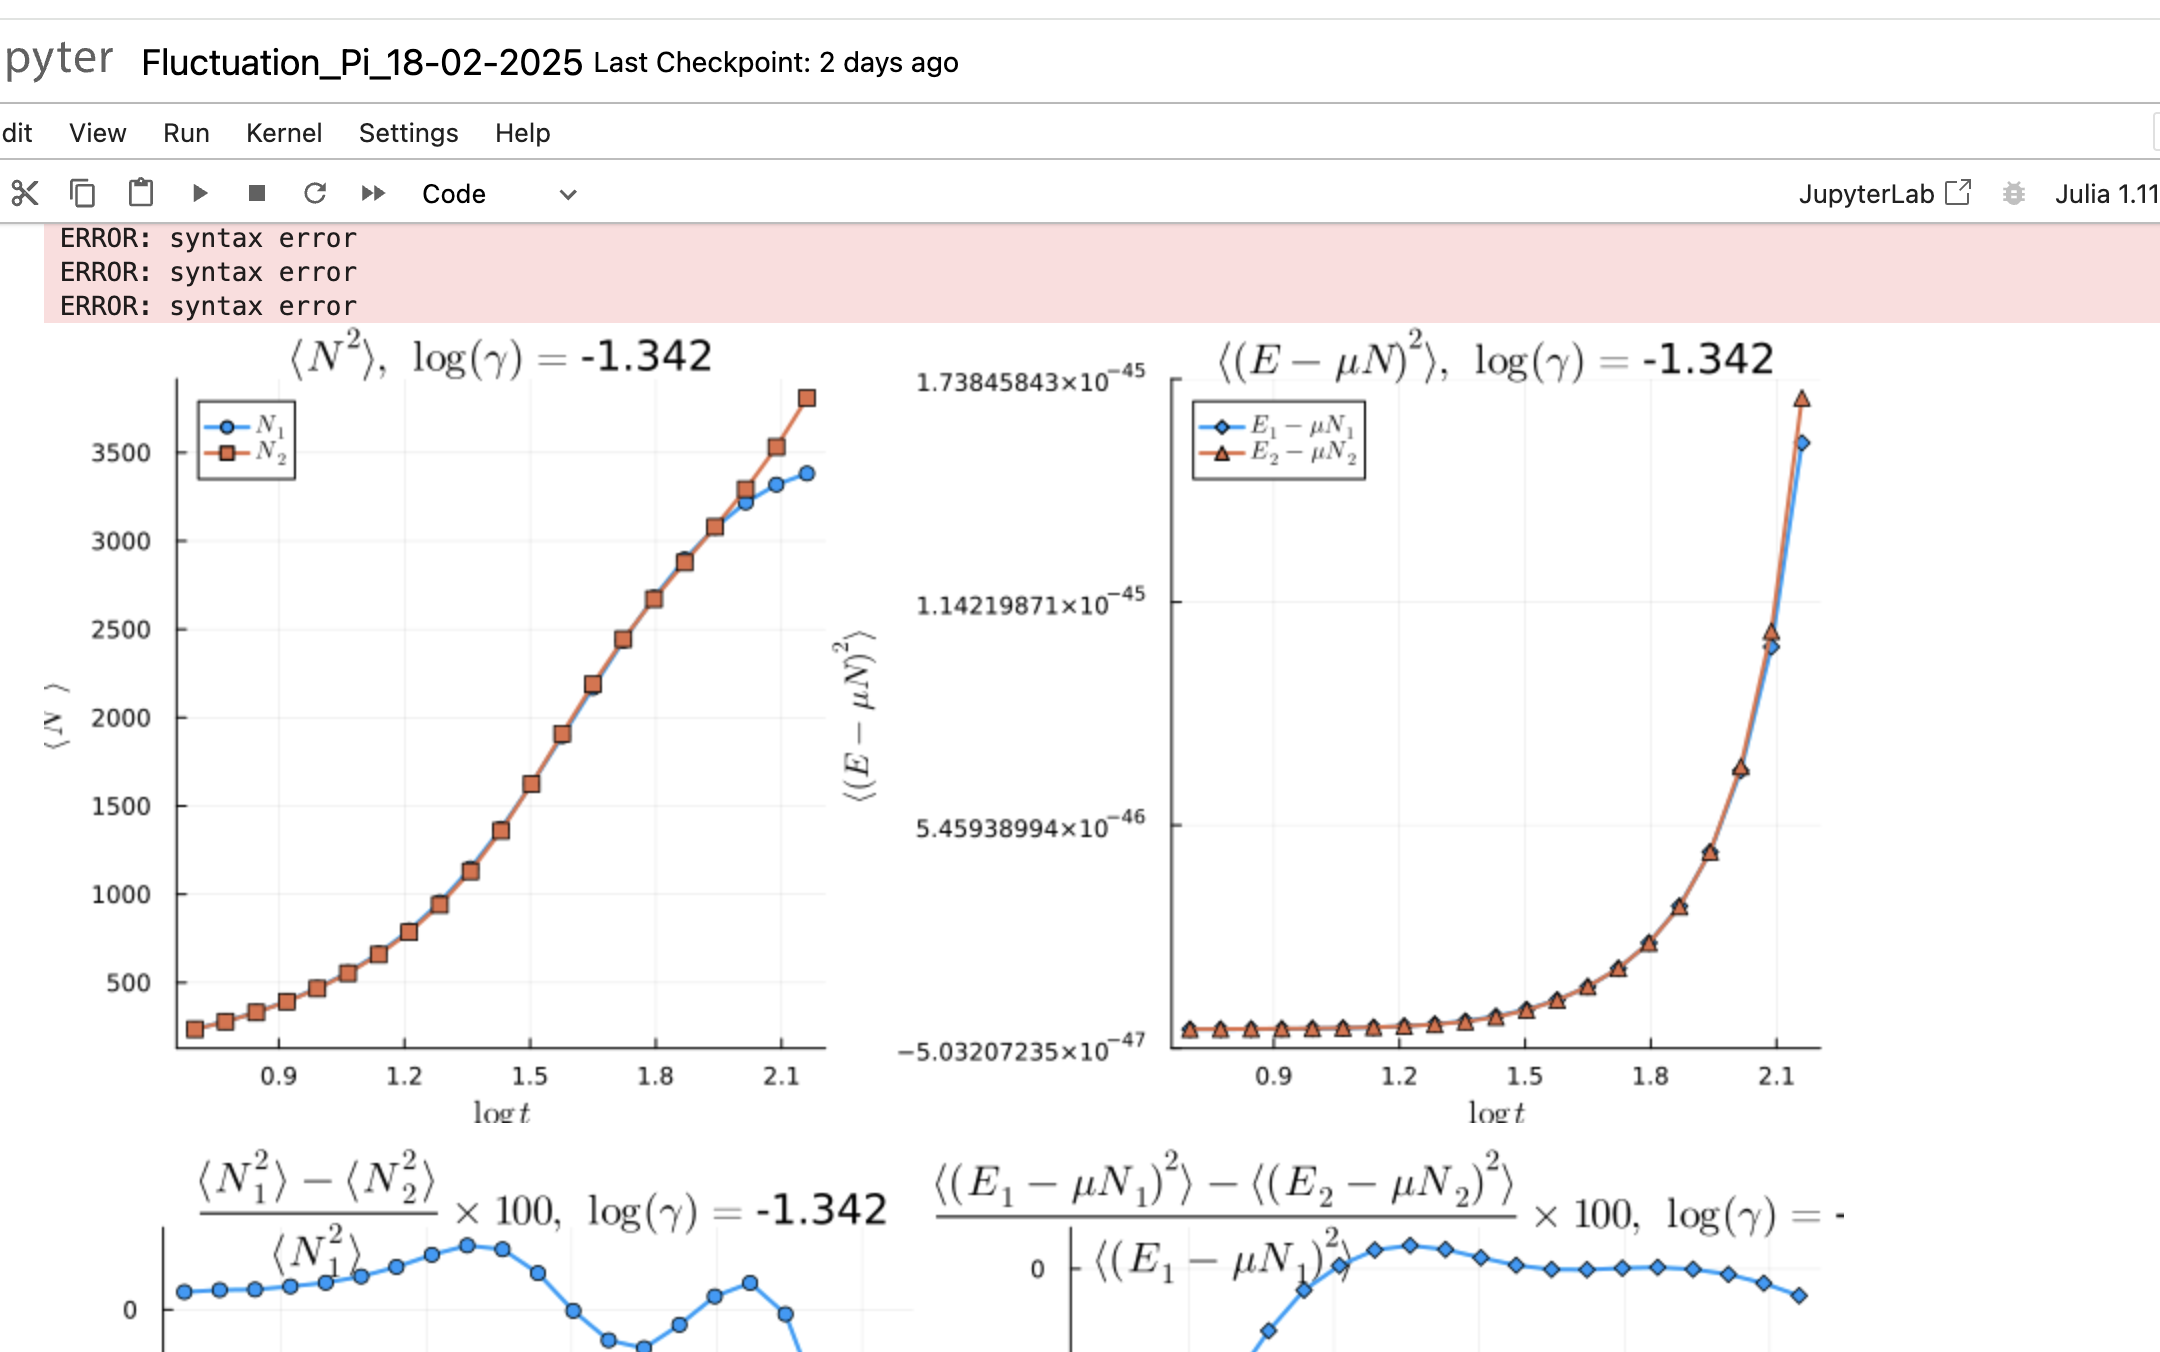
\includegraphics[width=1\textwidth]{Figures/test}

%\begin{aff}
%Donc une a l'ordre un en $\delta \theta (\operator{A}^{(0)})^{-1} %\operator{V}$ 

%\begin{eqnarray*}
%	\langle \delta \Pi ( \theta) \delta \Pi ( \theta') \rangle & = &  ( (\Pi^c_s - \Pi^c)\Pi^c/\Pi^c_s ) ( \theta ) \delta_{\theta, \theta'}/\delta \theta + \mathscr{F}(\theta , \theta' ) ,	
%\end{eqnarray*}

%avec 

%\begin{eqnarray*}
%	\mathscr{F}(\theta , \theta' ) & = & \left [ (\Pi^c_s - \Pi^c )( \theta)  +  (\Pi^c_s - \Pi^c ) ( \theta' )\right ] \frac{\Pi^c}{\Pi^c_s}(\theta)\frac{\Pi^c}{\Pi^c_s}(\theta') \frac{ \Delta( \theta'- \theta )}{ 2 \pi }\\
%	&&  - \left [ (\Pi^c_s - \Pi^c )( \theta)   (\Pi^c_s - \Pi^c ) ( \theta' )\right ] \frac{\Pi^c}{\Pi^c_s}(\theta)\frac{\Pi^c}{\Pi^c_s}(\theta')\int d\theta'' \left (   \frac{ \Pi^c/\Pi^c_s}{\Pi^c_s - \Pi^c} \right )(\theta'') \frac{\Delta(\theta''- \theta)}{2 \pi}\frac{\Delta(\theta''- \theta')}{2 \pi}  	
%\end{eqnarray*}
%\end{aff}



 









\subsection{Hamiltonien du modèle}
%Dans ce chapitre, nous nous intéressons aux fluctuations de la distribution de rapidité \( \delta \rho \) autour d'une distribution de référence \( \rho^c \), qui maximise la contribution à la fonction de partition des états, exprimée comme une fonctionnelle de la distribution \( \rho \) : 

La fonction de partition des états, s'exprime comme une fonctionnelle de la distribution \( \rho \) : 

\begin{eqnarray*}
	\Xi & = & \sum_\rho \exp \left( -\mathcal{A}(\rho) \right).
\end{eqnarray*}  

Dans la section {\em \bf Entropie de Yang-Yang} (\ref{??}), l'action \( \mathcal{A}(\rho) \) s'écrit sous la forme :  

\begin{eqnarray*}
	\mathcal{A}(\rho) & \doteq & - L\mathcal{S}_{YY}(\rho) + L\int f(\theta) \rho (\theta) \, d\theta,		
\end{eqnarray*}  

où \( \mathcal{S}_{YY} \) est la fonctionnelle d'entropie de Yang-Yang, définie dans (\ref{??}), et \( f \) est la fonction paramétrant les charges, introduite dans (\ref{??}).  

Dans cette même section {\em \bf Entropie de Yang-Yang} (\ref{??}), nous avons établi un lien entre \( f \) et distribution de référence \( \rho^c \), qui maximise la contribution à la fonction de partition des états .\\

On veux tester si nos experience est décrit pas un GGE. Pour cela nous nous intéressons aux fluctuations de la distribution de rapidité \( \delta \rho \) autour \( \rho^c \).

%Nous poursuivons à présent avec cette définition de l'action de classe $\mathcal{C}^2$ et admetant une distribution critique $\rho^c$ tel que sa différentielle en ce point critique soit nulle $d\mathcal{A}_{\rho^c} = 0 $ (\ref{??}) de sorte que d'aprés la formule de Taylor-Youg %afin de déterminer les fluctuations autour de \( \Pi^c \). Pour cela, nous réécrivons l'action sous la forme :  

Nous poursuivons à présent avec cette définition de l'action de classe $\mathcal{C}^2$ et admetant une distribution critique $\rho^c$ tel que sa différentielle en ce point critique soit nulle $d\mathcal{A}_{\rho^c} = 0 $ (\ref{??}) de sorte que d'aprés la formule de Taylor-Youg %afin de déterminer les fluctuations autour de \( \Pi^c \). Pour cela, nous réécrivons l'action sous la forme :  

\begin{eqnarray*}  
	\mathcal{A}(\rho^c + \delta \rho) & \underset{ \delta \rho \to 0 }{=} & \mathcal{A}(\rho^c)  + \frac{1}{2} \left. \frac{\delta^2 \mathcal{A}}{\delta \rho^2} \right|_{\rho^c} (\delta \rho) + \mathcal{O}((\delta \rho)^3),  
\end{eqnarray*}  

une expression quadratique pour l'action à l'ordre dominant en \( \delta \Pi \) avec $\left. \frac{\delta^2 \mathcal{A}}{\delta \rho^2} \right|_{\rho^c}$ la forme quadratique définie positive (Fig (\ref{fig.fluctu.A})).

\begin{figure}[H]
	\centering 
	\begin{tikzpicture}
		\begin{scope}[shift={(0,0)}]
			\begin{scope}[transform canvas={scale=0.6}]
				% Définition des couleurs avec les codes HTML
\definecolor{colorOne}{HTML}{443E46}
\definecolor{colorTwo}{HTML}{F6DEB8}
\definecolor{colorThree}{HTML}{908CA4}
\definecolor{colorFour}{HTML}{57659E}
\definecolor{colorFive}{HTML}{C57284}
\definecolor{colorSix}{HTML}{FF5B69}

% Raccourcis pour les couleurs
\def\colorOne{colorOne}
\def\colorTwo{colorTwo}
\def\colorThree{colorThree}
\def\colorFour{colorFour}
\def\colorFive{colorFive}
\def\colorSix{colorSix}

\def\colorslide{blue!50!black}



\begin{scope}
	% Tracer une courbe lisse entre des points
	\draw[shift={(0,0)} ,\colorOne]
		(-1 , 0 ) edge [thick,line width=0.8ex , ->,>=triangle 45  , \colorOne] node [pos = 1 , below ]{\huge$\rho$}( 5  , 0 )
	;
	\draw[shift={(0,0)}, color=\colorOne]
		(0, -1.0 ) edge [thick,line width=0.8ex , ->,>=triangle 45  ]node [pos=0.9,left=0.2cm ]{\huge$\mathcal{A}(\rho)$}( 0  , 5 )
	;
	\draw[]
		(2.5, 0.12 ) edge [thick,line width=0.8ex ,\colorThree ]node [pos=1,below  ]{\huge$\rho^c$} (2.5, -0.12 )	
	;
	
	\draw[]
		(2.5, -0.12 ) edge [thick,line width=0.4ex , dashed, \colorThree ] (2.5, 5.5 )
		(1.5, 1 ) edge [thick,line width=0.4ex , <->,>=triangle 45  , \colorThree ] (3.5, 1 )
		(-0.3,1) edge [thick,line width=0.4ex  , \colorThree ] node [pos=0,left ]{\huge$\mathcal{A}(\rho^c)$} (0.3, 1 )	
	;
    \draw[thick, line width=0.8ex , \colorFour] plot[smooth, tension=0.7] coordinates {
        (1, 5) (1.6 , 3 ) (2.5, 1) (3.5 , 3 )  (4, 5)
    };		
	
\end{scope}

	
			
			\end{scope}
			
			\draw[color = red , scale = 0.5 , draw = none  ] (-2 , -1) rectangle (5, 6) ; 	
		\end{scope}
		
		\begin{scope}[shift={(19,-1)}]
			\begin{scope}[transform canvas={scale=0.6}]
				% Définition des couleurs avec les codes HTML
\definecolor{colorOne}{HTML}{443E46}
\definecolor{colorTwo}{HTML}{F6DEB8}
\definecolor{colorThree}{HTML}{908CA4}
\definecolor{colorFour}{HTML}{57659E}
\definecolor{colorFive}{HTML}{C57284}
\definecolor{colorSix}{HTML}{FF5B69}

% Raccourcis pour les couleurs
\def\colorOne{colorOne}
\def\colorTwo{colorTwo}
\def\colorThree{colorThree}
\def\colorFour{colorFour}
\def\colorFive{colorFive}
\def\colorSix{colorSix}

\def\colorslide{blue!50!black}

\def\Occupation{
	\def\traitx{0.3}
	\def\traity{0.5}
	\draw[shift={(0,0)}]
		(-13.5 , 0 ) edge [thick,line width=0.8ex ]( -3.2  , 0 )
		( -3.2 - \traitx  , 0 - \traity ) edge [thick,line width=0.8ex ]( -3.2 + \traitx  , 0 + \traity  )
		( -2.8 - \traitx  , 0 - \traity ) edge [thick,line width=0.8ex ]( -2.8 + \traitx  , 0 + \traity  )
		(-2.8 , 0 ) edge [thick,line width=0.8ex ](2.8  , 0 )
		( 2.8 - \traitx  , 0 - \traity ) edge [thick,line width=0.8ex ]( 2.8 + \traitx  , 0 + \traity  )
		( 3.2 - \traitx  , 0 - \traity ) edge [thick,line width=0.8ex ]( 3.2 + \traitx  , 0 + \traity  )
		(3.2, 0 ) edge [thick,line width=0.8ex,->,>=triangle 45 , color = black ]node [pos=1.01,below  ]{\huge$\theta$}	( 13  , 0 )
	;
	\draw[shift={(0,0)}, color=\colorOne]
		(-10.5 , -1.5 ) edge [thick,line width=0.8ex , ->,>=triangle 45  ]( -10.5  , 4.5 )
	;
		
	\foreach \r in {1 , ... , 3 } {
%		\draw[
%		decoration={
%		markings,
%    	mark connection node=my node,
%    	mark=at position 0 with{\node [blue,transform shape] (my node) {\large \r};}},
%		color=gray, thick, 
%		line width=0.5ex] decorate { 
%            (-11.0, \r) -- (-10.1, \r )}
%        ;
        \draw[
			color=\colorOne,
			] 
            (-11.0, \r) edge[color=\colorThree , thick,line width=0.5ex] node [pos=-0.5 ]{\large\color{\colorFour} $\frac{\r}{\delta \theta}$ } (-10.3, \r )
        	;
	
	}
	

	
	% Graduation abcsisse 
	% Définitions des listes
% Definitions of the lists
\def\listetuple{-9/\theta_{1}, -8/\theta_{2} , -5/\theta_{3} , -2/\theta_{a-1} , 0/\theta_{a} , 1/\theta_{a+1} , 2/\theta_{a+2} ,  5/\theta_{N-4} , 7/\theta_{N-3},8/\theta_{N-1},9/\theta_{N} }
\def\listetrais{-12 , -11, -10, -9 , -8 , -7 ,  -6 , -5, -4.5,-4, -2 , -1, 0 , 0.5, 1, 2, 4 , 5 ,  6 , 7 , 8 ,8.5, 9 ,  10 , 11, 12 }

% Loop over listetrais
\foreach \r in \listetrais {
    % Initialize found variable to zero
    % Initialize found variable to zero
    %\pgfmathsetmacro\found{0}
    \global\def\found{0}
    \xdef\nomtheta{}
    
    % Check if \r is in listetuple
    \foreach \x/\y in \listetuple { 
        \ifdim \r pt=\x pt % If \r matches any \x in listetuple
            \global\def\found{1} ;
            \xdef\nomtheta{\y} % Set \nomtheta to the corresponding \y
            %\pgfmathsetmacro\found{1} % Set found to 1            
            %\global\pgfmathsetmacro\found{1}
        \fi
    }
    
    %\node [circle, draw, red] (A) at (\r, 2) {\found , $\nomtheta$};
    
    % Draw the line and display \nomtheta if found
    \ifnum\found=1
        \draw[color=\colorOne, thick, line width=0.5ex] 
            (\r, -0.3) -- (\r, 0.3) node[red , pos=-0.5] {\large $\nomtheta$};
         \filldraw[line width=0.5ex, color=\colorSix, outer color=\colorSix, inner color=\colorSix] 
            (\r, 0) circle (4pt);
    \else 
        % Draw without \nomtheta and add a blue circle if not found
        \draw[color=\colorOne, thick, line width=0.5ex] 
            (\r, -0.3) -- (\r, 0.3);
        \filldraw[line width=0.5ex, color=\colorSix, outer color=\colorTwo, inner color=\colorTwo] 
            (\r, 0) circle (4pt); 
    \fi
}

\def\listetrais{-9.5/\theta_{i-1}/2/3, -6.5/\theta_{i}/1/4  ,   -1.5/\theta_{j}/2/4 , 1.5/\theta_{j+1}/-1/3 , 3.5/\theta_{\ell-1}/1/3 , 6.5/\theta_{\ell}/3/4 , 9.5/\theta(\theta_{\ell+1})/-1/3 };



\foreach \r/\nomx/\y/\ys in \listetrais {
	\draw[
		decoration={
		markings,
    	mark connection node=my node,
    	mark=at position .5 with{\node [blue,transform shape] (my node) {\large \color{\colorFour} $\nomx$};}},
		color=\colorThree , thick, 
		line width=0.5ex] decorate { 
            (\r, 0.12) -- (\r, -1.2)}
        ;
     
     \ifdim \y pt > -1 pt 
     	\draw[
			decoration={
			markings,
    		mark connection node=my node,
    		mark=at position .5 with{\node [blue,transform shape] (my node) {\large \color{\colorFour} $\Pi(\nomx) $};}},
			color=\colorThree, thick, 
			line width=0.5ex] decorate { 
            (\r, \y) -- (\r +3, \y)}
        ;
        \draw[
			decoration={
			markings,
    		mark connection node=my node,
    		mark=at position .5 with{\node [blue,transform shape] (my node) {\large \color{\colorFive} $\Pi_s(\nomx) $};}},
			color=\colorFive, thick, 
			line width=0.5ex] decorate { 
            (\r, \ys) -- (\r +3, \ys)}
        ;
     \fi 
     \ifdim \r pt= -1.5 pt
     	\draw[
     		decoration={
			markings,
    		mark connection node=my node,
    		mark=at position .5 with{\node [blue,transform shape] (my node) {\large \color{\colorFour}  $\delta \theta $};},
    		%mark=at position 0.1  with {\arrow[blue, line width=0.5ex]{<}},
    		%mark=at position 1  with {\arrow[blue, line width=0.5ex]{>}}
    		},
        	color=\colorThree,
        	thick,
        	line width=0.5ex,
        	%arrows={Computer Modern Rightarrow[line cap=round]-Computer Modern Rightarrow[line cap=round]}
   			](\r, -1.2) edge[arrows={Computer Modern Rightarrow[line cap=round]-}] (\r + 0.4, -1.2)decorate {
    		(\r, -1.2) -- (\r + 3, -1.2)}(\r + 2, -1.2) edge[arrows={-Computer Modern Rightarrow[line cap=round]}] (\r + 3, -1.2)
    		;
    \fi
			
	
}


			
}


\begin{scope}
	%\draw[help lines , width=1.5ex] (-8,-3) grid (8,3);\draw[help lines ,width=0.5ex , opacity = 0.5] (-3,-3) grid[step=0.1] (3,3));
	
	%\draw[help lines] 
	%	(-3,-3) edge[width=1.5ex] grid (3,3)	
	%	(-3,-3) edge[width=0.5ex , opacity = 0.5] grid (3,3)	
	%;
	\begin{scope}[shift={(0,1)},rotate=0,opacity=1,color=black]
		\Occupation	
		
		%\node[anchor=east, font=\bfseries] at (-11, 0) {\color{red}\large (T = 0 )} ;	
	\end{scope}
	
	
	
	
	\begin{scope}[shift={(-10.5,7)},rotate=0,opacity=1,color=black]
	
	\begin{scope}[shift={(-0,0)},rotate=0,opacity=1,color=black]
	
		\draw[shift={(0,0)} ,line width=1ex,rounded corners = 1ex,color=\colorOne , opacity =1 ,fill=\colorOne!00 , pattern={north east lines} , pattern color=\colorOne!00 ]
			(0 , -1 ) rectangle (5,1)
		;
		

		\begin{scope}[shift={(0.5,0.5)}]
			\draw[color=\colorOne, thick, line width=0.5ex] 
            (0, -0.3) -- (0, 0.3) ;
            \filldraw[line width=0.5ex, color=\colorSix, outer color=\colorSix, inner color=\colorSix] 
            (0, 0) circle (4pt);
            
            \node[anchor=west, font=\bfseries] at (0.2, 0) {\color{\colorSix}\large : quasi-particule};
		\end{scope}
		
		\begin{scope}[shift={(0.5,-0.5)}]
			\draw[color=\colorOne, thick, line width=0.5ex] 
            (0, -0.3) -- (0, 0.3) ;
            \filldraw[line width=0.5ex, color=\colorSix, outer color=\colorTwo, inner color=\colorTwo] 
            (0, 0) circle (4pt);
            
            \node[anchor=west, font=\bfseries] at (0.2, 0) {\color{\colorSix}\large : hole};
		\end{scope}

	\end{scope}
	
	\begin{scope}[shift={(6,0)},rotate=0,opacity=1,color=black]	
		
		\draw[shift={(0,0)} ,line width=1ex,rounded corners = 1ex,color=\colorOne , opacity =1 ,fill=\colorOne!00 , pattern={north east lines} , pattern color=\colorOne!00 ]
			(0 , -1 ) rectangle (7.5,1)
		;
		
		\node[anchor=west] at (0.5, 0.5) {\color{\colorFour}\large $\Pi$ };\node[anchor=west, font=\bfseries] at (1, 0.5) {\color{\colorFour}\large : quasi-particule distribution};
		
		\node[anchor=west] at (0.5, -0.5) {\color{\colorFour}\large $\Pi_h$ };\node[anchor=west, font=\bfseries] at (1, -0.5) {\color{\colorFour}\large  : hole distribution};
		
	\end{scope}
	
	\begin{scope}[shift={(14.5,0)},rotate=0,opacity=1,color=black]	
		
		\draw[shift={(0,0)} ,line width=1ex,rounded corners = 1ex,color=\colorOne , opacity =1 ,fill=\colorOne!00 , pattern={north east lines} , pattern color=\colorOne!00 ]
			(0 , -0.5 ) rectangle (7.0,0.5)
		;
		
		\node[anchor=west] at (0.2, 0) {\color{\colorFour}\large ${\color{\colorFive}\Pi_s} = \Pi + \Pi_h $ } node[anchor=west , font=\bfseries] at (3.1 , 0 )  {\color{\colorFour}\large {\color{\colorFive} : density of states}};
		
	\end{scope}
	
	
	\end{scope}


		
	
\end{scope}

	
			
			\end{scope}
			\begin{scope}[scale=1]
				\draw[color = red , scale = 1 , draw = none  ] (-1 , -1) rectangle (5, 5) ; 
			\end{scope}	
		\end{scope}

		
				
			
	\end{tikzpicture}	
	\captionsetup{skip=10pt} % Ajoute de l’espace après la légende
	\label{fig.fluctu.A}
\end{figure}


On discrétise l'axe des rapidités en  petite cellule de rapidité $[\theta, \theta+\delta\theta]$, qui contient $L\rho(\theta) \delta \theta$ rapidités. 
	



Avec ces petites tranches, la forme quadratique s’écrit :

\begin{eqnarray*}
    \left. \frac{\delta^2 \mathcal{A}}{{\delta \rho}^2} \right|_{\rho^c}(\delta \rho ) &=&  \sum_{a,b \mid \text{tranche}}  
    \delta \rho(\theta_a)  \frac{\partial^2 \mathcal{A}}{\partial \delta \rho(\theta_a) \partial \delta \rho(\theta_b) } (\rho^c)  \delta \rho(\theta_b).
\end{eqnarray*}
Les fluctuations s’écrivent donc :

\begin{eqnarray*}
    \langle \delta \rho ( \theta) \delta \rho ( \theta') \rangle &=&  
    \frac{ \int d\delta \rho \, \delta \rho(\theta) \delta \rho ( \theta') 
    \exp \left( - \frac{1}{2} \sum_{a,b \mid \text{tranche}}  
    \delta \rho(\theta_a) \frac{\partial^2 \mathcal{A}}{\partial \delta \rho(\theta_a) \partial \delta \rho(\theta_b) } (\rho^c)  \delta \rho(\theta_b) \right) }
    { \int d\delta \Pi  
    \exp \left( - \frac{1}{2} \sum_{a,b \mid \text{tranche}}  
    \delta \rho(\theta_a) \frac{\partial^2 \mathcal{A}}{\partial \delta \rho(\theta_a) \partial \delta \rho(\theta_b) } (\rho^c)  \delta \rho(\theta_b) \right) } \\
    &=& \left( \mathbf{A}^{-1} \right)_{\theta , \theta'}
\end{eqnarray*}


\begin{aff}

\begin{eqnarray*}
	\langle \delta \rho ( \theta) \delta \rho ( \theta') \rangle &=& 	\left( \mathbf{A}^{-1} \right)_{\theta , \theta'}
\end{eqnarray*}

	
avec la  {\em matrice hessienne} $\mathbf{A}_{\theta , \theta'} \equiv \frac{\partial^2 \mathcal{A}}{\partial \delta \rho(\theta) \partial \delta \rho(\theta') }(\rho^c)$, au point critique/ qui maximise la probabilité  $\rho^c=\rho^c_s \nu^c $, s'écrit

\begin{eqnarray*}
	\operator{A} & = & \operator{A}^{(0)} + \delta \theta \operator{V}
\end{eqnarray*}

avec 

\begin{eqnarray*}
	A^{(0)}_{\theta , \theta'}  & = &  L\delta \theta \left ( \frac{ 1}{\rho^c_s ( 1  - \nu^c ) \nu^c } \right )(\theta)    \delta({\theta - \theta '})	,\\
	V_{\theta , \theta'}  &= & L \delta \theta \left \{ - \left [ \left ( \frac{1}{\rho^c_s( 1 - \nu^c) } \right ) ( \theta)  +  \left ( \frac{1}{\rho^c_s( 1 - \nu^c) } \right ) ( \theta' )\right ] \frac{ \Delta( \theta'- \theta )}{ 2 \pi } + \int d\theta''  \left ( \frac{\nu^c}{\rho^c_s( 1 - \nu^c) } \right )(\theta'') \frac{\Delta(\theta''- \theta)}{2 \pi}\frac{\Delta(\theta''- \theta')}{2 \pi}   \right \} 	
\end{eqnarray*}

\end{aff}

\subsection{Testes}

\begin{eqnarray*}
	\Delta_{\operator{\mathcal{N}}}^2  & = &  \frac{1}{\beta} \left . \frac{\partial \langle \operator{\mathcal{N}} \rangle}{\partial \mu} \right )_T \\
	\Delta_{\operator{\mathcal{E}}-\mu \operator{\mathcal{N}}}^2  & = &  - \left . \frac{\partial \langle \operator{\mathcal{E}}-\mu \operator{\mathcal{N}} \rangle}{\partial \beta} \right )_\mu 
\end{eqnarray*}

et 

\begin{eqnarray*}
	\Delta_{\operator{\mathcal{N}}}^2  &= & L^2 \int d\theta_a \int d \theta_b \, \langle \delta \rho(\theta_a) \delta \rho(\theta_b) \rangle \\
	\Delta_{\operator{\mathcal{E}}-\mu \operator{\mathcal{N}}}^2  & = & L^2 \int d\theta_a \int d \theta_b \, \left ( - \mu + \frac{1}2 m \theta_a^2  \right  )\left ( - \mu + \frac{1}2 m \theta_b^2  \right  )  \langle \delta \rho(\theta_a) \delta \rho(\theta_b) \rangle
\end{eqnarray*}

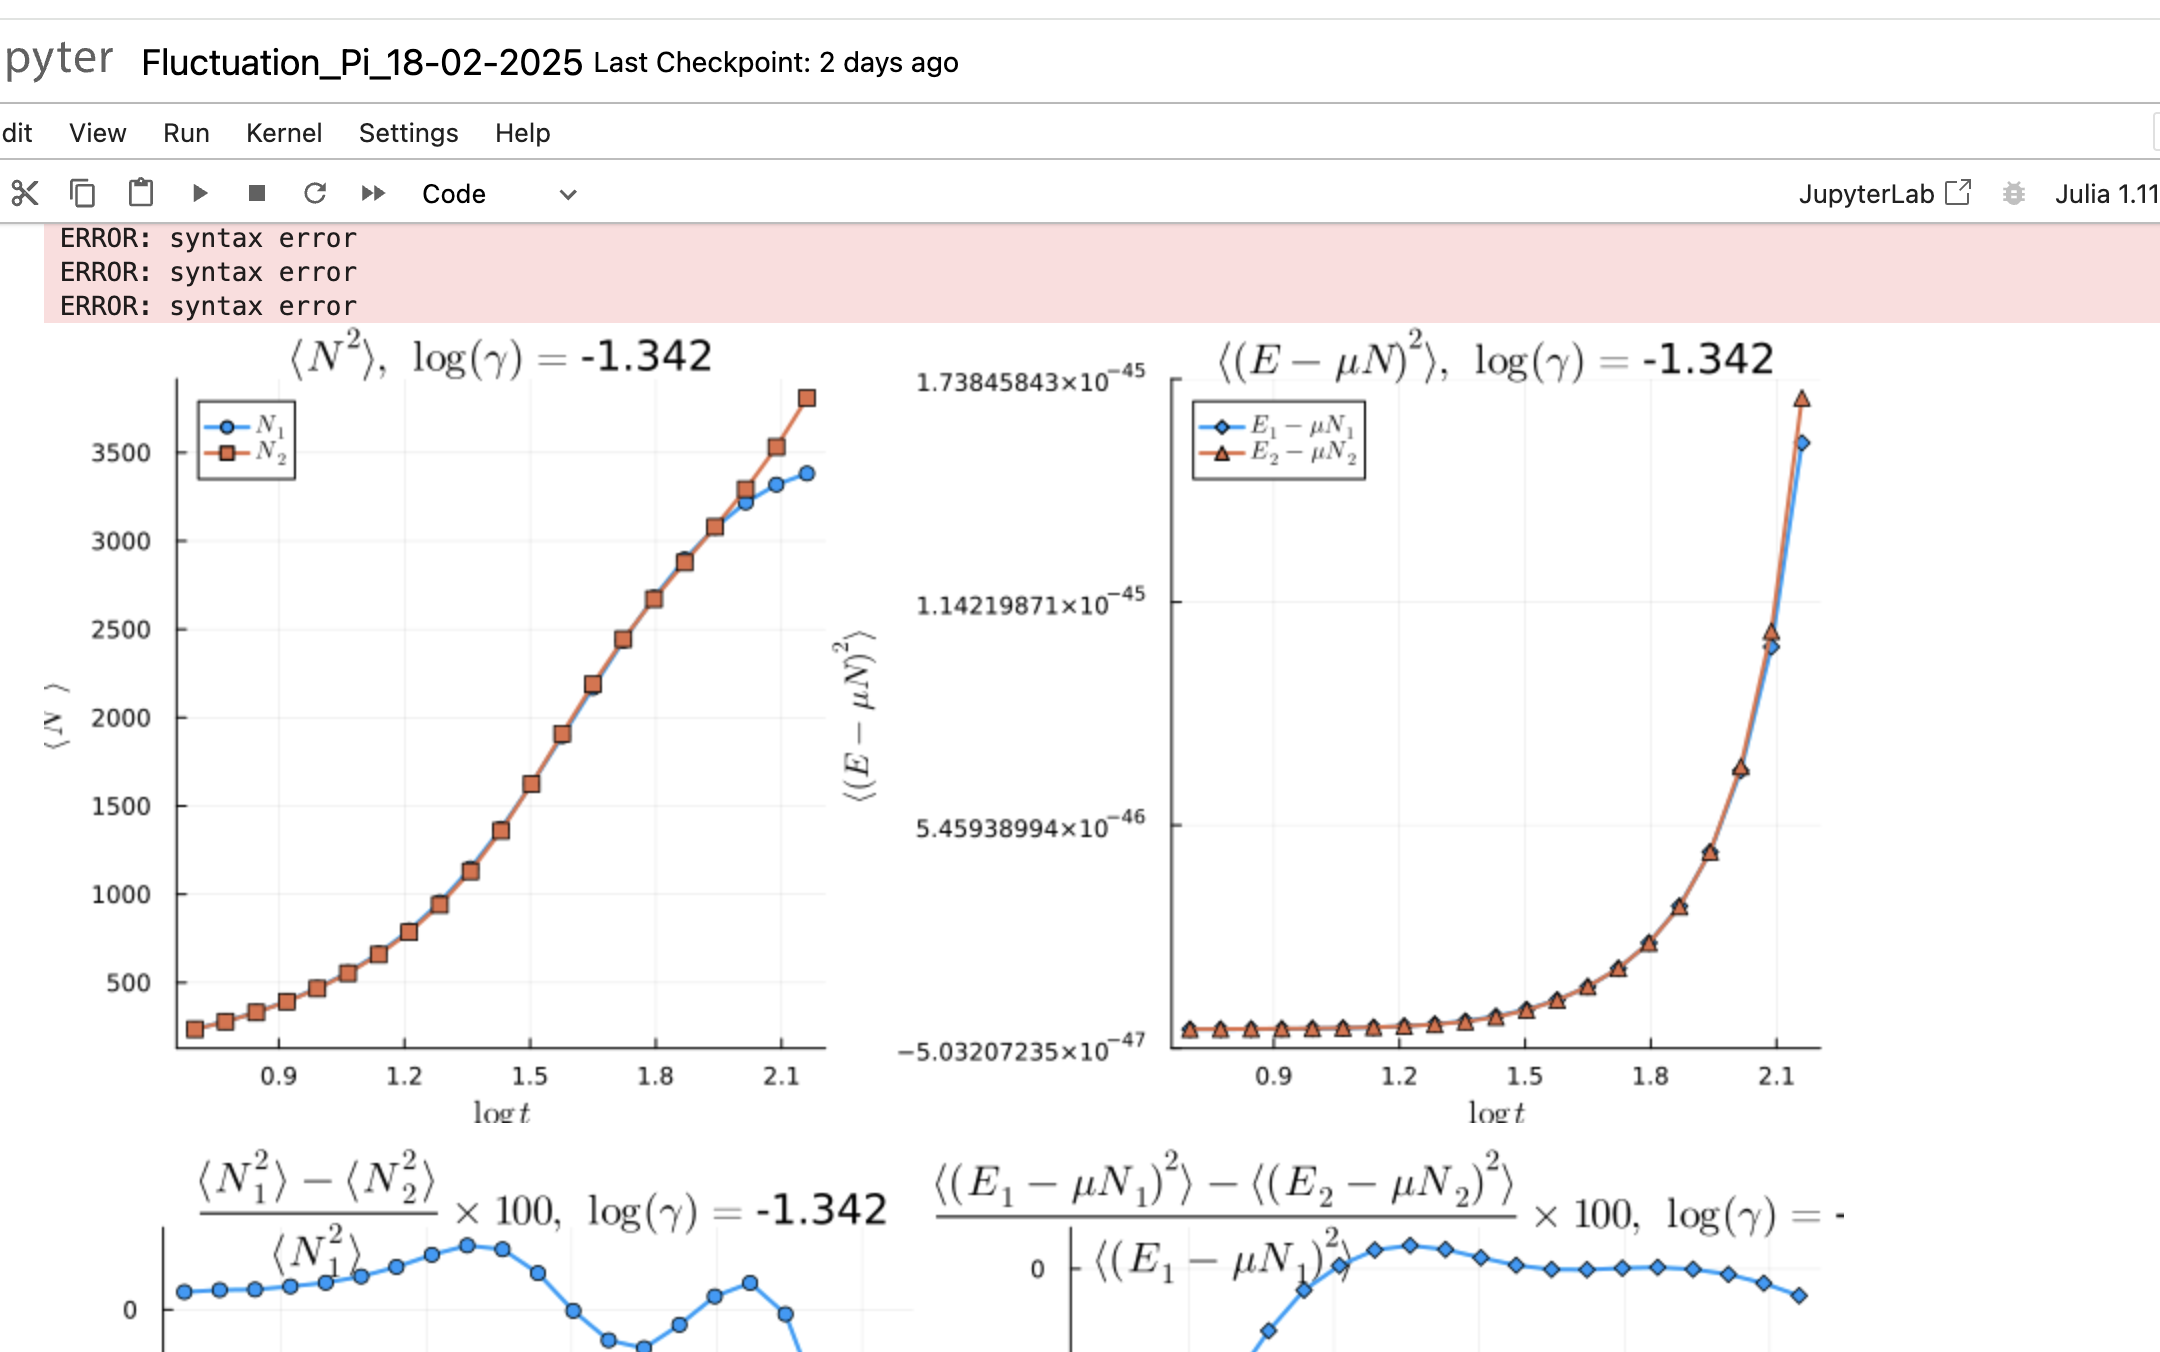
\includegraphics[width=1\textwidth]{Figures/test}

%\begin{aff}
%Donc une a l'ordre un en $\delta \theta (\operator{A}^{(0)})^{-1} %\operator{V}$ 

%\begin{eqnarray*}
%	\langle \delta \Pi ( \theta) \delta \Pi ( \theta') \rangle & = &  ( (\Pi^c_s - \Pi^c)\Pi^c/\Pi^c_s ) ( \theta ) \delta_{\theta, \theta'}/\delta \theta + \mathscr{F}(\theta , \theta' ) ,	
%\end{eqnarray*}

%avec 

%\begin{eqnarray*}
%	\mathscr{F}(\theta , \theta' ) & = & \left [ (\Pi^c_s - \Pi^c )( \theta)  +  (\Pi^c_s - \Pi^c ) ( \theta' )\right ] \frac{\Pi^c}{\Pi^c_s}(\theta)\frac{\Pi^c}{\Pi^c_s}(\theta') \frac{ \Delta( \theta'- \theta )}{ 2 \pi }\\
%	&&  - \left [ (\Pi^c_s - \Pi^c )( \theta)   (\Pi^c_s - \Pi^c ) ( \theta' )\right ] \frac{\Pi^c}{\Pi^c_s}(\theta)\frac{\Pi^c}{\Pi^c_s}(\theta')\int d\theta'' \left (   \frac{ \Pi^c/\Pi^c_s}{\Pi^c_s - \Pi^c} \right )(\theta'') \frac{\Delta(\theta''- \theta)}{2 \pi}\frac{\Delta(\theta''- \theta')}{2 \pi}  	
%\end{eqnarray*}
%\end{aff}



 









\subsection{États du vide et pseudovacuum}
%Dans ce chapitre, nous nous intéressons aux fluctuations de la distribution de rapidité \( \delta \rho \) autour d'une distribution de référence \( \rho^c \), qui maximise la contribution à la fonction de partition des états, exprimée comme une fonctionnelle de la distribution \( \rho \) : 

La fonction de partition des états, s'exprime comme une fonctionnelle de la distribution \( \rho \) : 

\begin{eqnarray*}
	\Xi & = & \sum_\rho \exp \left( -\mathcal{A}(\rho) \right).
\end{eqnarray*}  

Dans la section {\em \bf Entropie de Yang-Yang} (\ref{??}), l'action \( \mathcal{A}(\rho) \) s'écrit sous la forme :  

\begin{eqnarray*}
	\mathcal{A}(\rho) & \doteq & - L\mathcal{S}_{YY}(\rho) + L\int f(\theta) \rho (\theta) \, d\theta,		
\end{eqnarray*}  

où \( \mathcal{S}_{YY} \) est la fonctionnelle d'entropie de Yang-Yang, définie dans (\ref{??}), et \( f \) est la fonction paramétrant les charges, introduite dans (\ref{??}).  

Dans cette même section {\em \bf Entropie de Yang-Yang} (\ref{??}), nous avons établi un lien entre \( f \) et distribution de référence \( \rho^c \), qui maximise la contribution à la fonction de partition des états .\\

On veux tester si nos experience est décrit pas un GGE. Pour cela nous nous intéressons aux fluctuations de la distribution de rapidité \( \delta \rho \) autour \( \rho^c \).

%Nous poursuivons à présent avec cette définition de l'action de classe $\mathcal{C}^2$ et admetant une distribution critique $\rho^c$ tel que sa différentielle en ce point critique soit nulle $d\mathcal{A}_{\rho^c} = 0 $ (\ref{??}) de sorte que d'aprés la formule de Taylor-Youg %afin de déterminer les fluctuations autour de \( \Pi^c \). Pour cela, nous réécrivons l'action sous la forme :  

Nous poursuivons à présent avec cette définition de l'action de classe $\mathcal{C}^2$ et admetant une distribution critique $\rho^c$ tel que sa différentielle en ce point critique soit nulle $d\mathcal{A}_{\rho^c} = 0 $ (\ref{??}) de sorte que d'aprés la formule de Taylor-Youg %afin de déterminer les fluctuations autour de \( \Pi^c \). Pour cela, nous réécrivons l'action sous la forme :  

\begin{eqnarray*}  
	\mathcal{A}(\rho^c + \delta \rho) & \underset{ \delta \rho \to 0 }{=} & \mathcal{A}(\rho^c)  + \frac{1}{2} \left. \frac{\delta^2 \mathcal{A}}{\delta \rho^2} \right|_{\rho^c} (\delta \rho) + \mathcal{O}((\delta \rho)^3),  
\end{eqnarray*}  

une expression quadratique pour l'action à l'ordre dominant en \( \delta \Pi \) avec $\left. \frac{\delta^2 \mathcal{A}}{\delta \rho^2} \right|_{\rho^c}$ la forme quadratique définie positive (Fig (\ref{fig.fluctu.A})).

\begin{figure}[H]
	\centering 
	\begin{tikzpicture}
		\begin{scope}[shift={(0,0)}]
			\begin{scope}[transform canvas={scale=0.6}]
				% Définition des couleurs avec les codes HTML
\definecolor{colorOne}{HTML}{443E46}
\definecolor{colorTwo}{HTML}{F6DEB8}
\definecolor{colorThree}{HTML}{908CA4}
\definecolor{colorFour}{HTML}{57659E}
\definecolor{colorFive}{HTML}{C57284}
\definecolor{colorSix}{HTML}{FF5B69}

% Raccourcis pour les couleurs
\def\colorOne{colorOne}
\def\colorTwo{colorTwo}
\def\colorThree{colorThree}
\def\colorFour{colorFour}
\def\colorFive{colorFive}
\def\colorSix{colorSix}

\def\colorslide{blue!50!black}



\begin{scope}
	% Tracer une courbe lisse entre des points
	\draw[shift={(0,0)} ,\colorOne]
		(-1 , 0 ) edge [thick,line width=0.8ex , ->,>=triangle 45  , \colorOne] node [pos = 1 , below ]{\huge$\rho$}( 5  , 0 )
	;
	\draw[shift={(0,0)}, color=\colorOne]
		(0, -1.0 ) edge [thick,line width=0.8ex , ->,>=triangle 45  ]node [pos=0.9,left=0.2cm ]{\huge$\mathcal{A}(\rho)$}( 0  , 5 )
	;
	\draw[]
		(2.5, 0.12 ) edge [thick,line width=0.8ex ,\colorThree ]node [pos=1,below  ]{\huge$\rho^c$} (2.5, -0.12 )	
	;
	
	\draw[]
		(2.5, -0.12 ) edge [thick,line width=0.4ex , dashed, \colorThree ] (2.5, 5.5 )
		(1.5, 1 ) edge [thick,line width=0.4ex , <->,>=triangle 45  , \colorThree ] (3.5, 1 )
		(-0.3,1) edge [thick,line width=0.4ex  , \colorThree ] node [pos=0,left ]{\huge$\mathcal{A}(\rho^c)$} (0.3, 1 )	
	;
    \draw[thick, line width=0.8ex , \colorFour] plot[smooth, tension=0.7] coordinates {
        (1, 5) (1.6 , 3 ) (2.5, 1) (3.5 , 3 )  (4, 5)
    };		
	
\end{scope}

	
			
			\end{scope}
			
			\draw[color = red , scale = 0.5 , draw = none  ] (-2 , -1) rectangle (5, 6) ; 	
		\end{scope}
		
		\begin{scope}[shift={(19,-1)}]
			\begin{scope}[transform canvas={scale=0.6}]
				% Définition des couleurs avec les codes HTML
\definecolor{colorOne}{HTML}{443E46}
\definecolor{colorTwo}{HTML}{F6DEB8}
\definecolor{colorThree}{HTML}{908CA4}
\definecolor{colorFour}{HTML}{57659E}
\definecolor{colorFive}{HTML}{C57284}
\definecolor{colorSix}{HTML}{FF5B69}

% Raccourcis pour les couleurs
\def\colorOne{colorOne}
\def\colorTwo{colorTwo}
\def\colorThree{colorThree}
\def\colorFour{colorFour}
\def\colorFive{colorFive}
\def\colorSix{colorSix}

\def\colorslide{blue!50!black}

\def\Occupation{
	\def\traitx{0.3}
	\def\traity{0.5}
	\draw[shift={(0,0)}]
		(-13.5 , 0 ) edge [thick,line width=0.8ex ]( -3.2  , 0 )
		( -3.2 - \traitx  , 0 - \traity ) edge [thick,line width=0.8ex ]( -3.2 + \traitx  , 0 + \traity  )
		( -2.8 - \traitx  , 0 - \traity ) edge [thick,line width=0.8ex ]( -2.8 + \traitx  , 0 + \traity  )
		(-2.8 , 0 ) edge [thick,line width=0.8ex ](2.8  , 0 )
		( 2.8 - \traitx  , 0 - \traity ) edge [thick,line width=0.8ex ]( 2.8 + \traitx  , 0 + \traity  )
		( 3.2 - \traitx  , 0 - \traity ) edge [thick,line width=0.8ex ]( 3.2 + \traitx  , 0 + \traity  )
		(3.2, 0 ) edge [thick,line width=0.8ex,->,>=triangle 45 , color = black ]node [pos=1.01,below  ]{\huge$\theta$}	( 13  , 0 )
	;
	\draw[shift={(0,0)}, color=\colorOne]
		(-10.5 , -1.5 ) edge [thick,line width=0.8ex , ->,>=triangle 45  ]( -10.5  , 4.5 )
	;
		
	\foreach \r in {1 , ... , 3 } {
%		\draw[
%		decoration={
%		markings,
%    	mark connection node=my node,
%    	mark=at position 0 with{\node [blue,transform shape] (my node) {\large \r};}},
%		color=gray, thick, 
%		line width=0.5ex] decorate { 
%            (-11.0, \r) -- (-10.1, \r )}
%        ;
        \draw[
			color=\colorOne,
			] 
            (-11.0, \r) edge[color=\colorThree , thick,line width=0.5ex] node [pos=-0.5 ]{\large\color{\colorFour} $\frac{\r}{\delta \theta}$ } (-10.3, \r )
        	;
	
	}
	

	
	% Graduation abcsisse 
	% Définitions des listes
% Definitions of the lists
\def\listetuple{-9/\theta_{1}, -8/\theta_{2} , -5/\theta_{3} , -2/\theta_{a-1} , 0/\theta_{a} , 1/\theta_{a+1} , 2/\theta_{a+2} ,  5/\theta_{N-4} , 7/\theta_{N-3},8/\theta_{N-1},9/\theta_{N} }
\def\listetrais{-12 , -11, -10, -9 , -8 , -7 ,  -6 , -5, -4.5,-4, -2 , -1, 0 , 0.5, 1, 2, 4 , 5 ,  6 , 7 , 8 ,8.5, 9 ,  10 , 11, 12 }

% Loop over listetrais
\foreach \r in \listetrais {
    % Initialize found variable to zero
    % Initialize found variable to zero
    %\pgfmathsetmacro\found{0}
    \global\def\found{0}
    \xdef\nomtheta{}
    
    % Check if \r is in listetuple
    \foreach \x/\y in \listetuple { 
        \ifdim \r pt=\x pt % If \r matches any \x in listetuple
            \global\def\found{1} ;
            \xdef\nomtheta{\y} % Set \nomtheta to the corresponding \y
            %\pgfmathsetmacro\found{1} % Set found to 1            
            %\global\pgfmathsetmacro\found{1}
        \fi
    }
    
    %\node [circle, draw, red] (A) at (\r, 2) {\found , $\nomtheta$};
    
    % Draw the line and display \nomtheta if found
    \ifnum\found=1
        \draw[color=\colorOne, thick, line width=0.5ex] 
            (\r, -0.3) -- (\r, 0.3) node[red , pos=-0.5] {\large $\nomtheta$};
         \filldraw[line width=0.5ex, color=\colorSix, outer color=\colorSix, inner color=\colorSix] 
            (\r, 0) circle (4pt);
    \else 
        % Draw without \nomtheta and add a blue circle if not found
        \draw[color=\colorOne, thick, line width=0.5ex] 
            (\r, -0.3) -- (\r, 0.3);
        \filldraw[line width=0.5ex, color=\colorSix, outer color=\colorTwo, inner color=\colorTwo] 
            (\r, 0) circle (4pt); 
    \fi
}

\def\listetrais{-9.5/\theta_{i-1}/2/3, -6.5/\theta_{i}/1/4  ,   -1.5/\theta_{j}/2/4 , 1.5/\theta_{j+1}/-1/3 , 3.5/\theta_{\ell-1}/1/3 , 6.5/\theta_{\ell}/3/4 , 9.5/\theta(\theta_{\ell+1})/-1/3 };



\foreach \r/\nomx/\y/\ys in \listetrais {
	\draw[
		decoration={
		markings,
    	mark connection node=my node,
    	mark=at position .5 with{\node [blue,transform shape] (my node) {\large \color{\colorFour} $\nomx$};}},
		color=\colorThree , thick, 
		line width=0.5ex] decorate { 
            (\r, 0.12) -- (\r, -1.2)}
        ;
     
     \ifdim \y pt > -1 pt 
     	\draw[
			decoration={
			markings,
    		mark connection node=my node,
    		mark=at position .5 with{\node [blue,transform shape] (my node) {\large \color{\colorFour} $\Pi(\nomx) $};}},
			color=\colorThree, thick, 
			line width=0.5ex] decorate { 
            (\r, \y) -- (\r +3, \y)}
        ;
        \draw[
			decoration={
			markings,
    		mark connection node=my node,
    		mark=at position .5 with{\node [blue,transform shape] (my node) {\large \color{\colorFive} $\Pi_s(\nomx) $};}},
			color=\colorFive, thick, 
			line width=0.5ex] decorate { 
            (\r, \ys) -- (\r +3, \ys)}
        ;
     \fi 
     \ifdim \r pt= -1.5 pt
     	\draw[
     		decoration={
			markings,
    		mark connection node=my node,
    		mark=at position .5 with{\node [blue,transform shape] (my node) {\large \color{\colorFour}  $\delta \theta $};},
    		%mark=at position 0.1  with {\arrow[blue, line width=0.5ex]{<}},
    		%mark=at position 1  with {\arrow[blue, line width=0.5ex]{>}}
    		},
        	color=\colorThree,
        	thick,
        	line width=0.5ex,
        	%arrows={Computer Modern Rightarrow[line cap=round]-Computer Modern Rightarrow[line cap=round]}
   			](\r, -1.2) edge[arrows={Computer Modern Rightarrow[line cap=round]-}] (\r + 0.4, -1.2)decorate {
    		(\r, -1.2) -- (\r + 3, -1.2)}(\r + 2, -1.2) edge[arrows={-Computer Modern Rightarrow[line cap=round]}] (\r + 3, -1.2)
    		;
    \fi
			
	
}


			
}


\begin{scope}
	%\draw[help lines , width=1.5ex] (-8,-3) grid (8,3);\draw[help lines ,width=0.5ex , opacity = 0.5] (-3,-3) grid[step=0.1] (3,3));
	
	%\draw[help lines] 
	%	(-3,-3) edge[width=1.5ex] grid (3,3)	
	%	(-3,-3) edge[width=0.5ex , opacity = 0.5] grid (3,3)	
	%;
	\begin{scope}[shift={(0,1)},rotate=0,opacity=1,color=black]
		\Occupation	
		
		%\node[anchor=east, font=\bfseries] at (-11, 0) {\color{red}\large (T = 0 )} ;	
	\end{scope}
	
	
	
	
	\begin{scope}[shift={(-10.5,7)},rotate=0,opacity=1,color=black]
	
	\begin{scope}[shift={(-0,0)},rotate=0,opacity=1,color=black]
	
		\draw[shift={(0,0)} ,line width=1ex,rounded corners = 1ex,color=\colorOne , opacity =1 ,fill=\colorOne!00 , pattern={north east lines} , pattern color=\colorOne!00 ]
			(0 , -1 ) rectangle (5,1)
		;
		

		\begin{scope}[shift={(0.5,0.5)}]
			\draw[color=\colorOne, thick, line width=0.5ex] 
            (0, -0.3) -- (0, 0.3) ;
            \filldraw[line width=0.5ex, color=\colorSix, outer color=\colorSix, inner color=\colorSix] 
            (0, 0) circle (4pt);
            
            \node[anchor=west, font=\bfseries] at (0.2, 0) {\color{\colorSix}\large : quasi-particule};
		\end{scope}
		
		\begin{scope}[shift={(0.5,-0.5)}]
			\draw[color=\colorOne, thick, line width=0.5ex] 
            (0, -0.3) -- (0, 0.3) ;
            \filldraw[line width=0.5ex, color=\colorSix, outer color=\colorTwo, inner color=\colorTwo] 
            (0, 0) circle (4pt);
            
            \node[anchor=west, font=\bfseries] at (0.2, 0) {\color{\colorSix}\large : hole};
		\end{scope}

	\end{scope}
	
	\begin{scope}[shift={(6,0)},rotate=0,opacity=1,color=black]	
		
		\draw[shift={(0,0)} ,line width=1ex,rounded corners = 1ex,color=\colorOne , opacity =1 ,fill=\colorOne!00 , pattern={north east lines} , pattern color=\colorOne!00 ]
			(0 , -1 ) rectangle (7.5,1)
		;
		
		\node[anchor=west] at (0.5, 0.5) {\color{\colorFour}\large $\Pi$ };\node[anchor=west, font=\bfseries] at (1, 0.5) {\color{\colorFour}\large : quasi-particule distribution};
		
		\node[anchor=west] at (0.5, -0.5) {\color{\colorFour}\large $\Pi_h$ };\node[anchor=west, font=\bfseries] at (1, -0.5) {\color{\colorFour}\large  : hole distribution};
		
	\end{scope}
	
	\begin{scope}[shift={(14.5,0)},rotate=0,opacity=1,color=black]	
		
		\draw[shift={(0,0)} ,line width=1ex,rounded corners = 1ex,color=\colorOne , opacity =1 ,fill=\colorOne!00 , pattern={north east lines} , pattern color=\colorOne!00 ]
			(0 , -0.5 ) rectangle (7.0,0.5)
		;
		
		\node[anchor=west] at (0.2, 0) {\color{\colorFour}\large ${\color{\colorFive}\Pi_s} = \Pi + \Pi_h $ } node[anchor=west , font=\bfseries] at (3.1 , 0 )  {\color{\colorFour}\large {\color{\colorFive} : density of states}};
		
	\end{scope}
	
	
	\end{scope}


		
	
\end{scope}

	
			
			\end{scope}
			\begin{scope}[scale=1]
				\draw[color = red , scale = 1 , draw = none  ] (-1 , -1) rectangle (5, 5) ; 
			\end{scope}	
		\end{scope}

		
				
			
	\end{tikzpicture}	
	\captionsetup{skip=10pt} % Ajoute de l’espace après la légende
	\label{fig.fluctu.A}
\end{figure}


On discrétise l'axe des rapidités en  petite cellule de rapidité $[\theta, \theta+\delta\theta]$, qui contient $L\rho(\theta) \delta \theta$ rapidités. 
	



Avec ces petites tranches, la forme quadratique s’écrit :

\begin{eqnarray*}
    \left. \frac{\delta^2 \mathcal{A}}{{\delta \rho}^2} \right|_{\rho^c}(\delta \rho ) &=&  \sum_{a,b \mid \text{tranche}}  
    \delta \rho(\theta_a)  \frac{\partial^2 \mathcal{A}}{\partial \delta \rho(\theta_a) \partial \delta \rho(\theta_b) } (\rho^c)  \delta \rho(\theta_b).
\end{eqnarray*}
Les fluctuations s’écrivent donc :

\begin{eqnarray*}
    \langle \delta \rho ( \theta) \delta \rho ( \theta') \rangle &=&  
    \frac{ \int d\delta \rho \, \delta \rho(\theta) \delta \rho ( \theta') 
    \exp \left( - \frac{1}{2} \sum_{a,b \mid \text{tranche}}  
    \delta \rho(\theta_a) \frac{\partial^2 \mathcal{A}}{\partial \delta \rho(\theta_a) \partial \delta \rho(\theta_b) } (\rho^c)  \delta \rho(\theta_b) \right) }
    { \int d\delta \Pi  
    \exp \left( - \frac{1}{2} \sum_{a,b \mid \text{tranche}}  
    \delta \rho(\theta_a) \frac{\partial^2 \mathcal{A}}{\partial \delta \rho(\theta_a) \partial \delta \rho(\theta_b) } (\rho^c)  \delta \rho(\theta_b) \right) } \\
    &=& \left( \mathbf{A}^{-1} \right)_{\theta , \theta'}
\end{eqnarray*}


\begin{aff}

\begin{eqnarray*}
	\langle \delta \rho ( \theta) \delta \rho ( \theta') \rangle &=& 	\left( \mathbf{A}^{-1} \right)_{\theta , \theta'}
\end{eqnarray*}

	
avec la  {\em matrice hessienne} $\mathbf{A}_{\theta , \theta'} \equiv \frac{\partial^2 \mathcal{A}}{\partial \delta \rho(\theta) \partial \delta \rho(\theta') }(\rho^c)$, au point critique/ qui maximise la probabilité  $\rho^c=\rho^c_s \nu^c $, s'écrit

\begin{eqnarray*}
	\operator{A} & = & \operator{A}^{(0)} + \delta \theta \operator{V}
\end{eqnarray*}

avec 

\begin{eqnarray*}
	A^{(0)}_{\theta , \theta'}  & = &  L\delta \theta \left ( \frac{ 1}{\rho^c_s ( 1  - \nu^c ) \nu^c } \right )(\theta)    \delta({\theta - \theta '})	,\\
	V_{\theta , \theta'}  &= & L \delta \theta \left \{ - \left [ \left ( \frac{1}{\rho^c_s( 1 - \nu^c) } \right ) ( \theta)  +  \left ( \frac{1}{\rho^c_s( 1 - \nu^c) } \right ) ( \theta' )\right ] \frac{ \Delta( \theta'- \theta )}{ 2 \pi } + \int d\theta''  \left ( \frac{\nu^c}{\rho^c_s( 1 - \nu^c) } \right )(\theta'') \frac{\Delta(\theta''- \theta)}{2 \pi}\frac{\Delta(\theta''- \theta')}{2 \pi}   \right \} 	
\end{eqnarray*}

\end{aff}

\subsection{Testes}

\begin{eqnarray*}
	\Delta_{\operator{\mathcal{N}}}^2  & = &  \frac{1}{\beta} \left . \frac{\partial \langle \operator{\mathcal{N}} \rangle}{\partial \mu} \right )_T \\
	\Delta_{\operator{\mathcal{E}}-\mu \operator{\mathcal{N}}}^2  & = &  - \left . \frac{\partial \langle \operator{\mathcal{E}}-\mu \operator{\mathcal{N}} \rangle}{\partial \beta} \right )_\mu 
\end{eqnarray*}

et 

\begin{eqnarray*}
	\Delta_{\operator{\mathcal{N}}}^2  &= & L^2 \int d\theta_a \int d \theta_b \, \langle \delta \rho(\theta_a) \delta \rho(\theta_b) \rangle \\
	\Delta_{\operator{\mathcal{E}}-\mu \operator{\mathcal{N}}}^2  & = & L^2 \int d\theta_a \int d \theta_b \, \left ( - \mu + \frac{1}2 m \theta_a^2  \right  )\left ( - \mu + \frac{1}2 m \theta_b^2  \right  )  \langle \delta \rho(\theta_a) \delta \rho(\theta_b) \rangle
\end{eqnarray*}

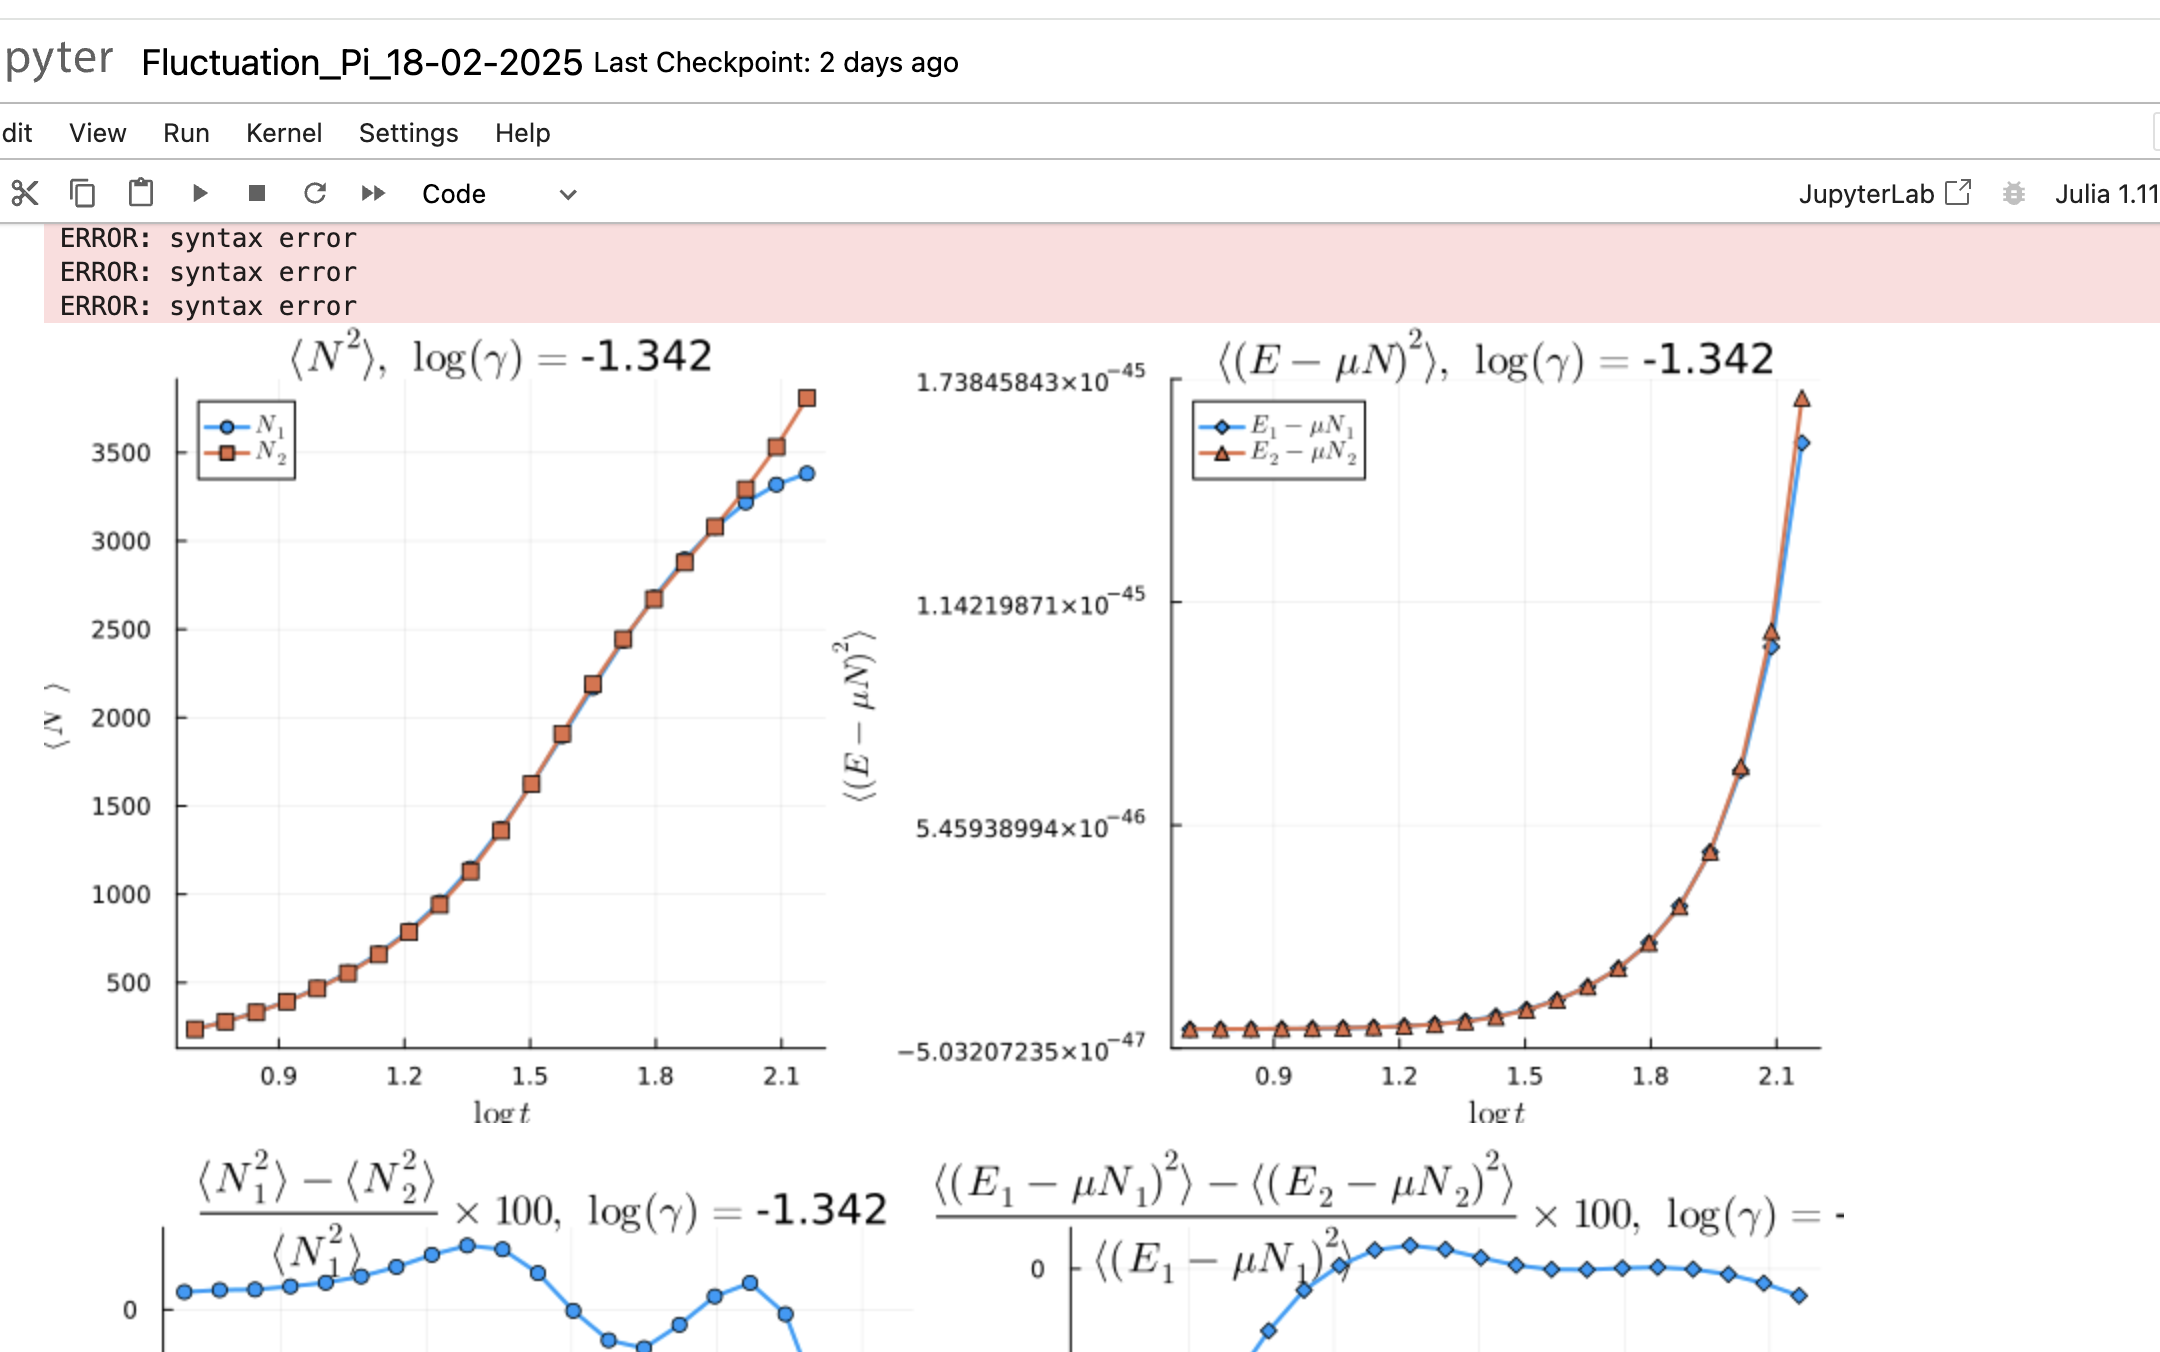
\includegraphics[width=1\textwidth]{Figures/test}

%\begin{aff}
%Donc une a l'ordre un en $\delta \theta (\operator{A}^{(0)})^{-1} %\operator{V}$ 

%\begin{eqnarray*}
%	\langle \delta \Pi ( \theta) \delta \Pi ( \theta') \rangle & = &  ( (\Pi^c_s - \Pi^c)\Pi^c/\Pi^c_s ) ( \theta ) \delta_{\theta, \theta'}/\delta \theta + \mathscr{F}(\theta , \theta' ) ,	
%\end{eqnarray*}

%avec 

%\begin{eqnarray*}
%	\mathscr{F}(\theta , \theta' ) & = & \left [ (\Pi^c_s - \Pi^c )( \theta)  +  (\Pi^c_s - \Pi^c ) ( \theta' )\right ] \frac{\Pi^c}{\Pi^c_s}(\theta)\frac{\Pi^c}{\Pi^c_s}(\theta') \frac{ \Delta( \theta'- \theta )}{ 2 \pi }\\
%	&&  - \left [ (\Pi^c_s - \Pi^c )( \theta)   (\Pi^c_s - \Pi^c ) ( \theta' )\right ] \frac{\Pi^c}{\Pi^c_s}(\theta)\frac{\Pi^c}{\Pi^c_s}(\theta')\int d\theta'' \left (   \frac{ \Pi^c/\Pi^c_s}{\Pi^c_s - \Pi^c} \right )(\theta'') \frac{\Delta(\theta''- \theta)}{2 \pi}\frac{\Delta(\theta''- \theta')}{2 \pi}  	
%\end{eqnarray*}
%\end{aff}



 










\subsection{Opérateurs conservés (intégrales du mouvement)}
%Dans ce chapitre, nous nous intéressons aux fluctuations de la distribution de rapidité \( \delta \rho \) autour d'une distribution de référence \( \rho^c \), qui maximise la contribution à la fonction de partition des états, exprimée comme une fonctionnelle de la distribution \( \rho \) : 

La fonction de partition des états, s'exprime comme une fonctionnelle de la distribution \( \rho \) : 

\begin{eqnarray*}
	\Xi & = & \sum_\rho \exp \left( -\mathcal{A}(\rho) \right).
\end{eqnarray*}  

Dans la section {\em \bf Entropie de Yang-Yang} (\ref{??}), l'action \( \mathcal{A}(\rho) \) s'écrit sous la forme :  

\begin{eqnarray*}
	\mathcal{A}(\rho) & \doteq & - L\mathcal{S}_{YY}(\rho) + L\int f(\theta) \rho (\theta) \, d\theta,		
\end{eqnarray*}  

où \( \mathcal{S}_{YY} \) est la fonctionnelle d'entropie de Yang-Yang, définie dans (\ref{??}), et \( f \) est la fonction paramétrant les charges, introduite dans (\ref{??}).  

Dans cette même section {\em \bf Entropie de Yang-Yang} (\ref{??}), nous avons établi un lien entre \( f \) et distribution de référence \( \rho^c \), qui maximise la contribution à la fonction de partition des états .\\

On veux tester si nos experience est décrit pas un GGE. Pour cela nous nous intéressons aux fluctuations de la distribution de rapidité \( \delta \rho \) autour \( \rho^c \).

%Nous poursuivons à présent avec cette définition de l'action de classe $\mathcal{C}^2$ et admetant une distribution critique $\rho^c$ tel que sa différentielle en ce point critique soit nulle $d\mathcal{A}_{\rho^c} = 0 $ (\ref{??}) de sorte que d'aprés la formule de Taylor-Youg %afin de déterminer les fluctuations autour de \( \Pi^c \). Pour cela, nous réécrivons l'action sous la forme :  

Nous poursuivons à présent avec cette définition de l'action de classe $\mathcal{C}^2$ et admetant une distribution critique $\rho^c$ tel que sa différentielle en ce point critique soit nulle $d\mathcal{A}_{\rho^c} = 0 $ (\ref{??}) de sorte que d'aprés la formule de Taylor-Youg %afin de déterminer les fluctuations autour de \( \Pi^c \). Pour cela, nous réécrivons l'action sous la forme :  

\begin{eqnarray*}  
	\mathcal{A}(\rho^c + \delta \rho) & \underset{ \delta \rho \to 0 }{=} & \mathcal{A}(\rho^c)  + \frac{1}{2} \left. \frac{\delta^2 \mathcal{A}}{\delta \rho^2} \right|_{\rho^c} (\delta \rho) + \mathcal{O}((\delta \rho)^3),  
\end{eqnarray*}  

une expression quadratique pour l'action à l'ordre dominant en \( \delta \Pi \) avec $\left. \frac{\delta^2 \mathcal{A}}{\delta \rho^2} \right|_{\rho^c}$ la forme quadratique définie positive (Fig (\ref{fig.fluctu.A})).

\begin{figure}[H]
	\centering 
	\begin{tikzpicture}
		\begin{scope}[shift={(0,0)}]
			\begin{scope}[transform canvas={scale=0.6}]
				% Définition des couleurs avec les codes HTML
\definecolor{colorOne}{HTML}{443E46}
\definecolor{colorTwo}{HTML}{F6DEB8}
\definecolor{colorThree}{HTML}{908CA4}
\definecolor{colorFour}{HTML}{57659E}
\definecolor{colorFive}{HTML}{C57284}
\definecolor{colorSix}{HTML}{FF5B69}

% Raccourcis pour les couleurs
\def\colorOne{colorOne}
\def\colorTwo{colorTwo}
\def\colorThree{colorThree}
\def\colorFour{colorFour}
\def\colorFive{colorFive}
\def\colorSix{colorSix}

\def\colorslide{blue!50!black}



\begin{scope}
	% Tracer une courbe lisse entre des points
	\draw[shift={(0,0)} ,\colorOne]
		(-1 , 0 ) edge [thick,line width=0.8ex , ->,>=triangle 45  , \colorOne] node [pos = 1 , below ]{\huge$\rho$}( 5  , 0 )
	;
	\draw[shift={(0,0)}, color=\colorOne]
		(0, -1.0 ) edge [thick,line width=0.8ex , ->,>=triangle 45  ]node [pos=0.9,left=0.2cm ]{\huge$\mathcal{A}(\rho)$}( 0  , 5 )
	;
	\draw[]
		(2.5, 0.12 ) edge [thick,line width=0.8ex ,\colorThree ]node [pos=1,below  ]{\huge$\rho^c$} (2.5, -0.12 )	
	;
	
	\draw[]
		(2.5, -0.12 ) edge [thick,line width=0.4ex , dashed, \colorThree ] (2.5, 5.5 )
		(1.5, 1 ) edge [thick,line width=0.4ex , <->,>=triangle 45  , \colorThree ] (3.5, 1 )
		(-0.3,1) edge [thick,line width=0.4ex  , \colorThree ] node [pos=0,left ]{\huge$\mathcal{A}(\rho^c)$} (0.3, 1 )	
	;
    \draw[thick, line width=0.8ex , \colorFour] plot[smooth, tension=0.7] coordinates {
        (1, 5) (1.6 , 3 ) (2.5, 1) (3.5 , 3 )  (4, 5)
    };		
	
\end{scope}

	
			
			\end{scope}
			
			\draw[color = red , scale = 0.5 , draw = none  ] (-2 , -1) rectangle (5, 6) ; 	
		\end{scope}
		
		\begin{scope}[shift={(19,-1)}]
			\begin{scope}[transform canvas={scale=0.6}]
				% Définition des couleurs avec les codes HTML
\definecolor{colorOne}{HTML}{443E46}
\definecolor{colorTwo}{HTML}{F6DEB8}
\definecolor{colorThree}{HTML}{908CA4}
\definecolor{colorFour}{HTML}{57659E}
\definecolor{colorFive}{HTML}{C57284}
\definecolor{colorSix}{HTML}{FF5B69}

% Raccourcis pour les couleurs
\def\colorOne{colorOne}
\def\colorTwo{colorTwo}
\def\colorThree{colorThree}
\def\colorFour{colorFour}
\def\colorFive{colorFive}
\def\colorSix{colorSix}

\def\colorslide{blue!50!black}

\def\Occupation{
	\def\traitx{0.3}
	\def\traity{0.5}
	\draw[shift={(0,0)}]
		(-13.5 , 0 ) edge [thick,line width=0.8ex ]( -3.2  , 0 )
		( -3.2 - \traitx  , 0 - \traity ) edge [thick,line width=0.8ex ]( -3.2 + \traitx  , 0 + \traity  )
		( -2.8 - \traitx  , 0 - \traity ) edge [thick,line width=0.8ex ]( -2.8 + \traitx  , 0 + \traity  )
		(-2.8 , 0 ) edge [thick,line width=0.8ex ](2.8  , 0 )
		( 2.8 - \traitx  , 0 - \traity ) edge [thick,line width=0.8ex ]( 2.8 + \traitx  , 0 + \traity  )
		( 3.2 - \traitx  , 0 - \traity ) edge [thick,line width=0.8ex ]( 3.2 + \traitx  , 0 + \traity  )
		(3.2, 0 ) edge [thick,line width=0.8ex,->,>=triangle 45 , color = black ]node [pos=1.01,below  ]{\huge$\theta$}	( 13  , 0 )
	;
	\draw[shift={(0,0)}, color=\colorOne]
		(-10.5 , -1.5 ) edge [thick,line width=0.8ex , ->,>=triangle 45  ]( -10.5  , 4.5 )
	;
		
	\foreach \r in {1 , ... , 3 } {
%		\draw[
%		decoration={
%		markings,
%    	mark connection node=my node,
%    	mark=at position 0 with{\node [blue,transform shape] (my node) {\large \r};}},
%		color=gray, thick, 
%		line width=0.5ex] decorate { 
%            (-11.0, \r) -- (-10.1, \r )}
%        ;
        \draw[
			color=\colorOne,
			] 
            (-11.0, \r) edge[color=\colorThree , thick,line width=0.5ex] node [pos=-0.5 ]{\large\color{\colorFour} $\frac{\r}{\delta \theta}$ } (-10.3, \r )
        	;
	
	}
	

	
	% Graduation abcsisse 
	% Définitions des listes
% Definitions of the lists
\def\listetuple{-9/\theta_{1}, -8/\theta_{2} , -5/\theta_{3} , -2/\theta_{a-1} , 0/\theta_{a} , 1/\theta_{a+1} , 2/\theta_{a+2} ,  5/\theta_{N-4} , 7/\theta_{N-3},8/\theta_{N-1},9/\theta_{N} }
\def\listetrais{-12 , -11, -10, -9 , -8 , -7 ,  -6 , -5, -4.5,-4, -2 , -1, 0 , 0.5, 1, 2, 4 , 5 ,  6 , 7 , 8 ,8.5, 9 ,  10 , 11, 12 }

% Loop over listetrais
\foreach \r in \listetrais {
    % Initialize found variable to zero
    % Initialize found variable to zero
    %\pgfmathsetmacro\found{0}
    \global\def\found{0}
    \xdef\nomtheta{}
    
    % Check if \r is in listetuple
    \foreach \x/\y in \listetuple { 
        \ifdim \r pt=\x pt % If \r matches any \x in listetuple
            \global\def\found{1} ;
            \xdef\nomtheta{\y} % Set \nomtheta to the corresponding \y
            %\pgfmathsetmacro\found{1} % Set found to 1            
            %\global\pgfmathsetmacro\found{1}
        \fi
    }
    
    %\node [circle, draw, red] (A) at (\r, 2) {\found , $\nomtheta$};
    
    % Draw the line and display \nomtheta if found
    \ifnum\found=1
        \draw[color=\colorOne, thick, line width=0.5ex] 
            (\r, -0.3) -- (\r, 0.3) node[red , pos=-0.5] {\large $\nomtheta$};
         \filldraw[line width=0.5ex, color=\colorSix, outer color=\colorSix, inner color=\colorSix] 
            (\r, 0) circle (4pt);
    \else 
        % Draw without \nomtheta and add a blue circle if not found
        \draw[color=\colorOne, thick, line width=0.5ex] 
            (\r, -0.3) -- (\r, 0.3);
        \filldraw[line width=0.5ex, color=\colorSix, outer color=\colorTwo, inner color=\colorTwo] 
            (\r, 0) circle (4pt); 
    \fi
}

\def\listetrais{-9.5/\theta_{i-1}/2/3, -6.5/\theta_{i}/1/4  ,   -1.5/\theta_{j}/2/4 , 1.5/\theta_{j+1}/-1/3 , 3.5/\theta_{\ell-1}/1/3 , 6.5/\theta_{\ell}/3/4 , 9.5/\theta(\theta_{\ell+1})/-1/3 };



\foreach \r/\nomx/\y/\ys in \listetrais {
	\draw[
		decoration={
		markings,
    	mark connection node=my node,
    	mark=at position .5 with{\node [blue,transform shape] (my node) {\large \color{\colorFour} $\nomx$};}},
		color=\colorThree , thick, 
		line width=0.5ex] decorate { 
            (\r, 0.12) -- (\r, -1.2)}
        ;
     
     \ifdim \y pt > -1 pt 
     	\draw[
			decoration={
			markings,
    		mark connection node=my node,
    		mark=at position .5 with{\node [blue,transform shape] (my node) {\large \color{\colorFour} $\Pi(\nomx) $};}},
			color=\colorThree, thick, 
			line width=0.5ex] decorate { 
            (\r, \y) -- (\r +3, \y)}
        ;
        \draw[
			decoration={
			markings,
    		mark connection node=my node,
    		mark=at position .5 with{\node [blue,transform shape] (my node) {\large \color{\colorFive} $\Pi_s(\nomx) $};}},
			color=\colorFive, thick, 
			line width=0.5ex] decorate { 
            (\r, \ys) -- (\r +3, \ys)}
        ;
     \fi 
     \ifdim \r pt= -1.5 pt
     	\draw[
     		decoration={
			markings,
    		mark connection node=my node,
    		mark=at position .5 with{\node [blue,transform shape] (my node) {\large \color{\colorFour}  $\delta \theta $};},
    		%mark=at position 0.1  with {\arrow[blue, line width=0.5ex]{<}},
    		%mark=at position 1  with {\arrow[blue, line width=0.5ex]{>}}
    		},
        	color=\colorThree,
        	thick,
        	line width=0.5ex,
        	%arrows={Computer Modern Rightarrow[line cap=round]-Computer Modern Rightarrow[line cap=round]}
   			](\r, -1.2) edge[arrows={Computer Modern Rightarrow[line cap=round]-}] (\r + 0.4, -1.2)decorate {
    		(\r, -1.2) -- (\r + 3, -1.2)}(\r + 2, -1.2) edge[arrows={-Computer Modern Rightarrow[line cap=round]}] (\r + 3, -1.2)
    		;
    \fi
			
	
}


			
}


\begin{scope}
	%\draw[help lines , width=1.5ex] (-8,-3) grid (8,3);\draw[help lines ,width=0.5ex , opacity = 0.5] (-3,-3) grid[step=0.1] (3,3));
	
	%\draw[help lines] 
	%	(-3,-3) edge[width=1.5ex] grid (3,3)	
	%	(-3,-3) edge[width=0.5ex , opacity = 0.5] grid (3,3)	
	%;
	\begin{scope}[shift={(0,1)},rotate=0,opacity=1,color=black]
		\Occupation	
		
		%\node[anchor=east, font=\bfseries] at (-11, 0) {\color{red}\large (T = 0 )} ;	
	\end{scope}
	
	
	
	
	\begin{scope}[shift={(-10.5,7)},rotate=0,opacity=1,color=black]
	
	\begin{scope}[shift={(-0,0)},rotate=0,opacity=1,color=black]
	
		\draw[shift={(0,0)} ,line width=1ex,rounded corners = 1ex,color=\colorOne , opacity =1 ,fill=\colorOne!00 , pattern={north east lines} , pattern color=\colorOne!00 ]
			(0 , -1 ) rectangle (5,1)
		;
		

		\begin{scope}[shift={(0.5,0.5)}]
			\draw[color=\colorOne, thick, line width=0.5ex] 
            (0, -0.3) -- (0, 0.3) ;
            \filldraw[line width=0.5ex, color=\colorSix, outer color=\colorSix, inner color=\colorSix] 
            (0, 0) circle (4pt);
            
            \node[anchor=west, font=\bfseries] at (0.2, 0) {\color{\colorSix}\large : quasi-particule};
		\end{scope}
		
		\begin{scope}[shift={(0.5,-0.5)}]
			\draw[color=\colorOne, thick, line width=0.5ex] 
            (0, -0.3) -- (0, 0.3) ;
            \filldraw[line width=0.5ex, color=\colorSix, outer color=\colorTwo, inner color=\colorTwo] 
            (0, 0) circle (4pt);
            
            \node[anchor=west, font=\bfseries] at (0.2, 0) {\color{\colorSix}\large : hole};
		\end{scope}

	\end{scope}
	
	\begin{scope}[shift={(6,0)},rotate=0,opacity=1,color=black]	
		
		\draw[shift={(0,0)} ,line width=1ex,rounded corners = 1ex,color=\colorOne , opacity =1 ,fill=\colorOne!00 , pattern={north east lines} , pattern color=\colorOne!00 ]
			(0 , -1 ) rectangle (7.5,1)
		;
		
		\node[anchor=west] at (0.5, 0.5) {\color{\colorFour}\large $\Pi$ };\node[anchor=west, font=\bfseries] at (1, 0.5) {\color{\colorFour}\large : quasi-particule distribution};
		
		\node[anchor=west] at (0.5, -0.5) {\color{\colorFour}\large $\Pi_h$ };\node[anchor=west, font=\bfseries] at (1, -0.5) {\color{\colorFour}\large  : hole distribution};
		
	\end{scope}
	
	\begin{scope}[shift={(14.5,0)},rotate=0,opacity=1,color=black]	
		
		\draw[shift={(0,0)} ,line width=1ex,rounded corners = 1ex,color=\colorOne , opacity =1 ,fill=\colorOne!00 , pattern={north east lines} , pattern color=\colorOne!00 ]
			(0 , -0.5 ) rectangle (7.0,0.5)
		;
		
		\node[anchor=west] at (0.2, 0) {\color{\colorFour}\large ${\color{\colorFive}\Pi_s} = \Pi + \Pi_h $ } node[anchor=west , font=\bfseries] at (3.1 , 0 )  {\color{\colorFour}\large {\color{\colorFive} : density of states}};
		
	\end{scope}
	
	
	\end{scope}


		
	
\end{scope}

	
			
			\end{scope}
			\begin{scope}[scale=1]
				\draw[color = red , scale = 1 , draw = none  ] (-1 , -1) rectangle (5, 5) ; 
			\end{scope}	
		\end{scope}

		
				
			
	\end{tikzpicture}	
	\captionsetup{skip=10pt} % Ajoute de l’espace après la légende
	\label{fig.fluctu.A}
\end{figure}


On discrétise l'axe des rapidités en  petite cellule de rapidité $[\theta, \theta+\delta\theta]$, qui contient $L\rho(\theta) \delta \theta$ rapidités. 
	



Avec ces petites tranches, la forme quadratique s’écrit :

\begin{eqnarray*}
    \left. \frac{\delta^2 \mathcal{A}}{{\delta \rho}^2} \right|_{\rho^c}(\delta \rho ) &=&  \sum_{a,b \mid \text{tranche}}  
    \delta \rho(\theta_a)  \frac{\partial^2 \mathcal{A}}{\partial \delta \rho(\theta_a) \partial \delta \rho(\theta_b) } (\rho^c)  \delta \rho(\theta_b).
\end{eqnarray*}
Les fluctuations s’écrivent donc :

\begin{eqnarray*}
    \langle \delta \rho ( \theta) \delta \rho ( \theta') \rangle &=&  
    \frac{ \int d\delta \rho \, \delta \rho(\theta) \delta \rho ( \theta') 
    \exp \left( - \frac{1}{2} \sum_{a,b \mid \text{tranche}}  
    \delta \rho(\theta_a) \frac{\partial^2 \mathcal{A}}{\partial \delta \rho(\theta_a) \partial \delta \rho(\theta_b) } (\rho^c)  \delta \rho(\theta_b) \right) }
    { \int d\delta \Pi  
    \exp \left( - \frac{1}{2} \sum_{a,b \mid \text{tranche}}  
    \delta \rho(\theta_a) \frac{\partial^2 \mathcal{A}}{\partial \delta \rho(\theta_a) \partial \delta \rho(\theta_b) } (\rho^c)  \delta \rho(\theta_b) \right) } \\
    &=& \left( \mathbf{A}^{-1} \right)_{\theta , \theta'}
\end{eqnarray*}


\begin{aff}

\begin{eqnarray*}
	\langle \delta \rho ( \theta) \delta \rho ( \theta') \rangle &=& 	\left( \mathbf{A}^{-1} \right)_{\theta , \theta'}
\end{eqnarray*}

	
avec la  {\em matrice hessienne} $\mathbf{A}_{\theta , \theta'} \equiv \frac{\partial^2 \mathcal{A}}{\partial \delta \rho(\theta) \partial \delta \rho(\theta') }(\rho^c)$, au point critique/ qui maximise la probabilité  $\rho^c=\rho^c_s \nu^c $, s'écrit

\begin{eqnarray*}
	\operator{A} & = & \operator{A}^{(0)} + \delta \theta \operator{V}
\end{eqnarray*}

avec 

\begin{eqnarray*}
	A^{(0)}_{\theta , \theta'}  & = &  L\delta \theta \left ( \frac{ 1}{\rho^c_s ( 1  - \nu^c ) \nu^c } \right )(\theta)    \delta({\theta - \theta '})	,\\
	V_{\theta , \theta'}  &= & L \delta \theta \left \{ - \left [ \left ( \frac{1}{\rho^c_s( 1 - \nu^c) } \right ) ( \theta)  +  \left ( \frac{1}{\rho^c_s( 1 - \nu^c) } \right ) ( \theta' )\right ] \frac{ \Delta( \theta'- \theta )}{ 2 \pi } + \int d\theta''  \left ( \frac{\nu^c}{\rho^c_s( 1 - \nu^c) } \right )(\theta'') \frac{\Delta(\theta''- \theta)}{2 \pi}\frac{\Delta(\theta''- \theta')}{2 \pi}   \right \} 	
\end{eqnarray*}

\end{aff}

\subsection{Testes}

\begin{eqnarray*}
	\Delta_{\operator{\mathcal{N}}}^2  & = &  \frac{1}{\beta} \left . \frac{\partial \langle \operator{\mathcal{N}} \rangle}{\partial \mu} \right )_T \\
	\Delta_{\operator{\mathcal{E}}-\mu \operator{\mathcal{N}}}^2  & = &  - \left . \frac{\partial \langle \operator{\mathcal{E}}-\mu \operator{\mathcal{N}} \rangle}{\partial \beta} \right )_\mu 
\end{eqnarray*}

et 

\begin{eqnarray*}
	\Delta_{\operator{\mathcal{N}}}^2  &= & L^2 \int d\theta_a \int d \theta_b \, \langle \delta \rho(\theta_a) \delta \rho(\theta_b) \rangle \\
	\Delta_{\operator{\mathcal{E}}-\mu \operator{\mathcal{N}}}^2  & = & L^2 \int d\theta_a \int d \theta_b \, \left ( - \mu + \frac{1}2 m \theta_a^2  \right  )\left ( - \mu + \frac{1}2 m \theta_b^2  \right  )  \langle \delta \rho(\theta_a) \delta \rho(\theta_b) \rangle
\end{eqnarray*}

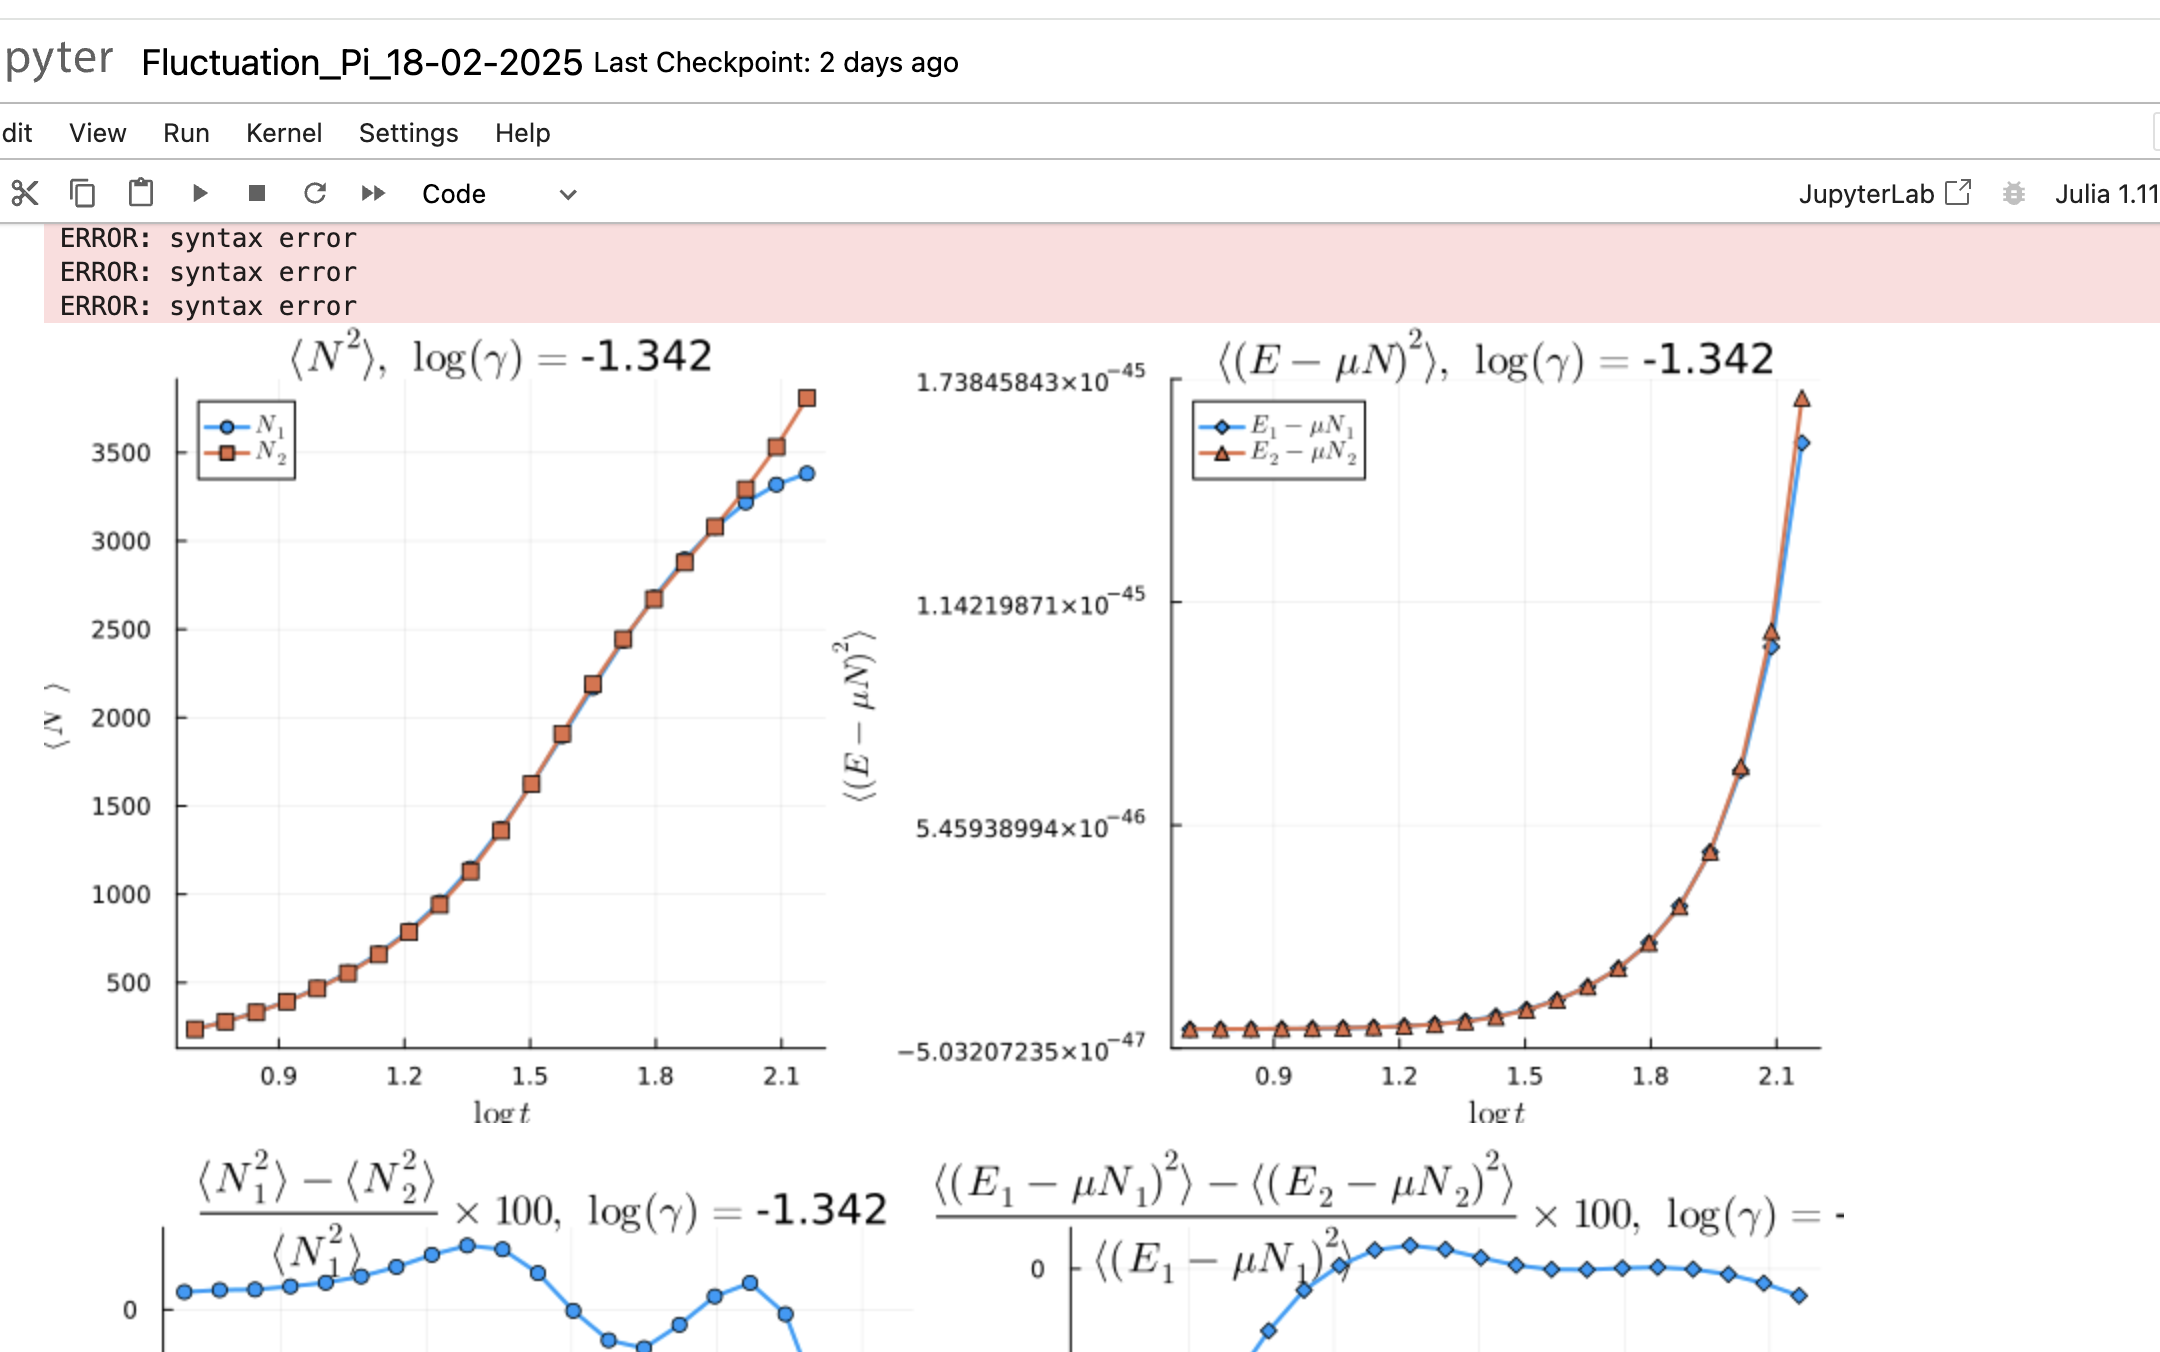
\includegraphics[width=1\textwidth]{Figures/test}

%\begin{aff}
%Donc une a l'ordre un en $\delta \theta (\operator{A}^{(0)})^{-1} %\operator{V}$ 

%\begin{eqnarray*}
%	\langle \delta \Pi ( \theta) \delta \Pi ( \theta') \rangle & = &  ( (\Pi^c_s - \Pi^c)\Pi^c/\Pi^c_s ) ( \theta ) \delta_{\theta, \theta'}/\delta \theta + \mathscr{F}(\theta , \theta' ) ,	
%\end{eqnarray*}

%avec 

%\begin{eqnarray*}
%	\mathscr{F}(\theta , \theta' ) & = & \left [ (\Pi^c_s - \Pi^c )( \theta)  +  (\Pi^c_s - \Pi^c ) ( \theta' )\right ] \frac{\Pi^c}{\Pi^c_s}(\theta)\frac{\Pi^c}{\Pi^c_s}(\theta') \frac{ \Delta( \theta'- \theta )}{ 2 \pi }\\
%	&&  - \left [ (\Pi^c_s - \Pi^c )( \theta)   (\Pi^c_s - \Pi^c ) ( \theta' )\right ] \frac{\Pi^c}{\Pi^c_s}(\theta)\frac{\Pi^c}{\Pi^c_s}(\theta')\int d\theta'' \left (   \frac{ \Pi^c/\Pi^c_s}{\Pi^c_s - \Pi^c} \right )(\theta'') \frac{\Delta(\theta''- \theta)}{2 \pi}\frac{\Delta(\theta''- \theta')}{2 \pi}  	
%\end{eqnarray*}
%\end{aff}



 








 
\subsection{Fonction d’onde $\chi_N$ et Hamiltonien et moment à N corps}
%Dans ce chapitre, nous nous intéressons aux fluctuations de la distribution de rapidité \( \delta \rho \) autour d'une distribution de référence \( \rho^c \), qui maximise la contribution à la fonction de partition des états, exprimée comme une fonctionnelle de la distribution \( \rho \) : 

La fonction de partition des états, s'exprime comme une fonctionnelle de la distribution \( \rho \) : 

\begin{eqnarray*}
	\Xi & = & \sum_\rho \exp \left( -\mathcal{A}(\rho) \right).
\end{eqnarray*}  

Dans la section {\em \bf Entropie de Yang-Yang} (\ref{??}), l'action \( \mathcal{A}(\rho) \) s'écrit sous la forme :  

\begin{eqnarray*}
	\mathcal{A}(\rho) & \doteq & - L\mathcal{S}_{YY}(\rho) + L\int f(\theta) \rho (\theta) \, d\theta,		
\end{eqnarray*}  

où \( \mathcal{S}_{YY} \) est la fonctionnelle d'entropie de Yang-Yang, définie dans (\ref{??}), et \( f \) est la fonction paramétrant les charges, introduite dans (\ref{??}).  

Dans cette même section {\em \bf Entropie de Yang-Yang} (\ref{??}), nous avons établi un lien entre \( f \) et distribution de référence \( \rho^c \), qui maximise la contribution à la fonction de partition des états .\\

On veux tester si nos experience est décrit pas un GGE. Pour cela nous nous intéressons aux fluctuations de la distribution de rapidité \( \delta \rho \) autour \( \rho^c \).

%Nous poursuivons à présent avec cette définition de l'action de classe $\mathcal{C}^2$ et admetant une distribution critique $\rho^c$ tel que sa différentielle en ce point critique soit nulle $d\mathcal{A}_{\rho^c} = 0 $ (\ref{??}) de sorte que d'aprés la formule de Taylor-Youg %afin de déterminer les fluctuations autour de \( \Pi^c \). Pour cela, nous réécrivons l'action sous la forme :  

Nous poursuivons à présent avec cette définition de l'action de classe $\mathcal{C}^2$ et admetant une distribution critique $\rho^c$ tel que sa différentielle en ce point critique soit nulle $d\mathcal{A}_{\rho^c} = 0 $ (\ref{??}) de sorte que d'aprés la formule de Taylor-Youg %afin de déterminer les fluctuations autour de \( \Pi^c \). Pour cela, nous réécrivons l'action sous la forme :  

\begin{eqnarray*}  
	\mathcal{A}(\rho^c + \delta \rho) & \underset{ \delta \rho \to 0 }{=} & \mathcal{A}(\rho^c)  + \frac{1}{2} \left. \frac{\delta^2 \mathcal{A}}{\delta \rho^2} \right|_{\rho^c} (\delta \rho) + \mathcal{O}((\delta \rho)^3),  
\end{eqnarray*}  

une expression quadratique pour l'action à l'ordre dominant en \( \delta \Pi \) avec $\left. \frac{\delta^2 \mathcal{A}}{\delta \rho^2} \right|_{\rho^c}$ la forme quadratique définie positive (Fig (\ref{fig.fluctu.A})).

\begin{figure}[H]
	\centering 
	\begin{tikzpicture}
		\begin{scope}[shift={(0,0)}]
			\begin{scope}[transform canvas={scale=0.6}]
				% Définition des couleurs avec les codes HTML
\definecolor{colorOne}{HTML}{443E46}
\definecolor{colorTwo}{HTML}{F6DEB8}
\definecolor{colorThree}{HTML}{908CA4}
\definecolor{colorFour}{HTML}{57659E}
\definecolor{colorFive}{HTML}{C57284}
\definecolor{colorSix}{HTML}{FF5B69}

% Raccourcis pour les couleurs
\def\colorOne{colorOne}
\def\colorTwo{colorTwo}
\def\colorThree{colorThree}
\def\colorFour{colorFour}
\def\colorFive{colorFive}
\def\colorSix{colorSix}

\def\colorslide{blue!50!black}



\begin{scope}
	% Tracer une courbe lisse entre des points
	\draw[shift={(0,0)} ,\colorOne]
		(-1 , 0 ) edge [thick,line width=0.8ex , ->,>=triangle 45  , \colorOne] node [pos = 1 , below ]{\huge$\rho$}( 5  , 0 )
	;
	\draw[shift={(0,0)}, color=\colorOne]
		(0, -1.0 ) edge [thick,line width=0.8ex , ->,>=triangle 45  ]node [pos=0.9,left=0.2cm ]{\huge$\mathcal{A}(\rho)$}( 0  , 5 )
	;
	\draw[]
		(2.5, 0.12 ) edge [thick,line width=0.8ex ,\colorThree ]node [pos=1,below  ]{\huge$\rho^c$} (2.5, -0.12 )	
	;
	
	\draw[]
		(2.5, -0.12 ) edge [thick,line width=0.4ex , dashed, \colorThree ] (2.5, 5.5 )
		(1.5, 1 ) edge [thick,line width=0.4ex , <->,>=triangle 45  , \colorThree ] (3.5, 1 )
		(-0.3,1) edge [thick,line width=0.4ex  , \colorThree ] node [pos=0,left ]{\huge$\mathcal{A}(\rho^c)$} (0.3, 1 )	
	;
    \draw[thick, line width=0.8ex , \colorFour] plot[smooth, tension=0.7] coordinates {
        (1, 5) (1.6 , 3 ) (2.5, 1) (3.5 , 3 )  (4, 5)
    };		
	
\end{scope}

	
			
			\end{scope}
			
			\draw[color = red , scale = 0.5 , draw = none  ] (-2 , -1) rectangle (5, 6) ; 	
		\end{scope}
		
		\begin{scope}[shift={(19,-1)}]
			\begin{scope}[transform canvas={scale=0.6}]
				% Définition des couleurs avec les codes HTML
\definecolor{colorOne}{HTML}{443E46}
\definecolor{colorTwo}{HTML}{F6DEB8}
\definecolor{colorThree}{HTML}{908CA4}
\definecolor{colorFour}{HTML}{57659E}
\definecolor{colorFive}{HTML}{C57284}
\definecolor{colorSix}{HTML}{FF5B69}

% Raccourcis pour les couleurs
\def\colorOne{colorOne}
\def\colorTwo{colorTwo}
\def\colorThree{colorThree}
\def\colorFour{colorFour}
\def\colorFive{colorFive}
\def\colorSix{colorSix}

\def\colorslide{blue!50!black}

\def\Occupation{
	\def\traitx{0.3}
	\def\traity{0.5}
	\draw[shift={(0,0)}]
		(-13.5 , 0 ) edge [thick,line width=0.8ex ]( -3.2  , 0 )
		( -3.2 - \traitx  , 0 - \traity ) edge [thick,line width=0.8ex ]( -3.2 + \traitx  , 0 + \traity  )
		( -2.8 - \traitx  , 0 - \traity ) edge [thick,line width=0.8ex ]( -2.8 + \traitx  , 0 + \traity  )
		(-2.8 , 0 ) edge [thick,line width=0.8ex ](2.8  , 0 )
		( 2.8 - \traitx  , 0 - \traity ) edge [thick,line width=0.8ex ]( 2.8 + \traitx  , 0 + \traity  )
		( 3.2 - \traitx  , 0 - \traity ) edge [thick,line width=0.8ex ]( 3.2 + \traitx  , 0 + \traity  )
		(3.2, 0 ) edge [thick,line width=0.8ex,->,>=triangle 45 , color = black ]node [pos=1.01,below  ]{\huge$\theta$}	( 13  , 0 )
	;
	\draw[shift={(0,0)}, color=\colorOne]
		(-10.5 , -1.5 ) edge [thick,line width=0.8ex , ->,>=triangle 45  ]( -10.5  , 4.5 )
	;
		
	\foreach \r in {1 , ... , 3 } {
%		\draw[
%		decoration={
%		markings,
%    	mark connection node=my node,
%    	mark=at position 0 with{\node [blue,transform shape] (my node) {\large \r};}},
%		color=gray, thick, 
%		line width=0.5ex] decorate { 
%            (-11.0, \r) -- (-10.1, \r )}
%        ;
        \draw[
			color=\colorOne,
			] 
            (-11.0, \r) edge[color=\colorThree , thick,line width=0.5ex] node [pos=-0.5 ]{\large\color{\colorFour} $\frac{\r}{\delta \theta}$ } (-10.3, \r )
        	;
	
	}
	

	
	% Graduation abcsisse 
	% Définitions des listes
% Definitions of the lists
\def\listetuple{-9/\theta_{1}, -8/\theta_{2} , -5/\theta_{3} , -2/\theta_{a-1} , 0/\theta_{a} , 1/\theta_{a+1} , 2/\theta_{a+2} ,  5/\theta_{N-4} , 7/\theta_{N-3},8/\theta_{N-1},9/\theta_{N} }
\def\listetrais{-12 , -11, -10, -9 , -8 , -7 ,  -6 , -5, -4.5,-4, -2 , -1, 0 , 0.5, 1, 2, 4 , 5 ,  6 , 7 , 8 ,8.5, 9 ,  10 , 11, 12 }

% Loop over listetrais
\foreach \r in \listetrais {
    % Initialize found variable to zero
    % Initialize found variable to zero
    %\pgfmathsetmacro\found{0}
    \global\def\found{0}
    \xdef\nomtheta{}
    
    % Check if \r is in listetuple
    \foreach \x/\y in \listetuple { 
        \ifdim \r pt=\x pt % If \r matches any \x in listetuple
            \global\def\found{1} ;
            \xdef\nomtheta{\y} % Set \nomtheta to the corresponding \y
            %\pgfmathsetmacro\found{1} % Set found to 1            
            %\global\pgfmathsetmacro\found{1}
        \fi
    }
    
    %\node [circle, draw, red] (A) at (\r, 2) {\found , $\nomtheta$};
    
    % Draw the line and display \nomtheta if found
    \ifnum\found=1
        \draw[color=\colorOne, thick, line width=0.5ex] 
            (\r, -0.3) -- (\r, 0.3) node[red , pos=-0.5] {\large $\nomtheta$};
         \filldraw[line width=0.5ex, color=\colorSix, outer color=\colorSix, inner color=\colorSix] 
            (\r, 0) circle (4pt);
    \else 
        % Draw without \nomtheta and add a blue circle if not found
        \draw[color=\colorOne, thick, line width=0.5ex] 
            (\r, -0.3) -- (\r, 0.3);
        \filldraw[line width=0.5ex, color=\colorSix, outer color=\colorTwo, inner color=\colorTwo] 
            (\r, 0) circle (4pt); 
    \fi
}

\def\listetrais{-9.5/\theta_{i-1}/2/3, -6.5/\theta_{i}/1/4  ,   -1.5/\theta_{j}/2/4 , 1.5/\theta_{j+1}/-1/3 , 3.5/\theta_{\ell-1}/1/3 , 6.5/\theta_{\ell}/3/4 , 9.5/\theta(\theta_{\ell+1})/-1/3 };



\foreach \r/\nomx/\y/\ys in \listetrais {
	\draw[
		decoration={
		markings,
    	mark connection node=my node,
    	mark=at position .5 with{\node [blue,transform shape] (my node) {\large \color{\colorFour} $\nomx$};}},
		color=\colorThree , thick, 
		line width=0.5ex] decorate { 
            (\r, 0.12) -- (\r, -1.2)}
        ;
     
     \ifdim \y pt > -1 pt 
     	\draw[
			decoration={
			markings,
    		mark connection node=my node,
    		mark=at position .5 with{\node [blue,transform shape] (my node) {\large \color{\colorFour} $\Pi(\nomx) $};}},
			color=\colorThree, thick, 
			line width=0.5ex] decorate { 
            (\r, \y) -- (\r +3, \y)}
        ;
        \draw[
			decoration={
			markings,
    		mark connection node=my node,
    		mark=at position .5 with{\node [blue,transform shape] (my node) {\large \color{\colorFive} $\Pi_s(\nomx) $};}},
			color=\colorFive, thick, 
			line width=0.5ex] decorate { 
            (\r, \ys) -- (\r +3, \ys)}
        ;
     \fi 
     \ifdim \r pt= -1.5 pt
     	\draw[
     		decoration={
			markings,
    		mark connection node=my node,
    		mark=at position .5 with{\node [blue,transform shape] (my node) {\large \color{\colorFour}  $\delta \theta $};},
    		%mark=at position 0.1  with {\arrow[blue, line width=0.5ex]{<}},
    		%mark=at position 1  with {\arrow[blue, line width=0.5ex]{>}}
    		},
        	color=\colorThree,
        	thick,
        	line width=0.5ex,
        	%arrows={Computer Modern Rightarrow[line cap=round]-Computer Modern Rightarrow[line cap=round]}
   			](\r, -1.2) edge[arrows={Computer Modern Rightarrow[line cap=round]-}] (\r + 0.4, -1.2)decorate {
    		(\r, -1.2) -- (\r + 3, -1.2)}(\r + 2, -1.2) edge[arrows={-Computer Modern Rightarrow[line cap=round]}] (\r + 3, -1.2)
    		;
    \fi
			
	
}


			
}


\begin{scope}
	%\draw[help lines , width=1.5ex] (-8,-3) grid (8,3);\draw[help lines ,width=0.5ex , opacity = 0.5] (-3,-3) grid[step=0.1] (3,3));
	
	%\draw[help lines] 
	%	(-3,-3) edge[width=1.5ex] grid (3,3)	
	%	(-3,-3) edge[width=0.5ex , opacity = 0.5] grid (3,3)	
	%;
	\begin{scope}[shift={(0,1)},rotate=0,opacity=1,color=black]
		\Occupation	
		
		%\node[anchor=east, font=\bfseries] at (-11, 0) {\color{red}\large (T = 0 )} ;	
	\end{scope}
	
	
	
	
	\begin{scope}[shift={(-10.5,7)},rotate=0,opacity=1,color=black]
	
	\begin{scope}[shift={(-0,0)},rotate=0,opacity=1,color=black]
	
		\draw[shift={(0,0)} ,line width=1ex,rounded corners = 1ex,color=\colorOne , opacity =1 ,fill=\colorOne!00 , pattern={north east lines} , pattern color=\colorOne!00 ]
			(0 , -1 ) rectangle (5,1)
		;
		

		\begin{scope}[shift={(0.5,0.5)}]
			\draw[color=\colorOne, thick, line width=0.5ex] 
            (0, -0.3) -- (0, 0.3) ;
            \filldraw[line width=0.5ex, color=\colorSix, outer color=\colorSix, inner color=\colorSix] 
            (0, 0) circle (4pt);
            
            \node[anchor=west, font=\bfseries] at (0.2, 0) {\color{\colorSix}\large : quasi-particule};
		\end{scope}
		
		\begin{scope}[shift={(0.5,-0.5)}]
			\draw[color=\colorOne, thick, line width=0.5ex] 
            (0, -0.3) -- (0, 0.3) ;
            \filldraw[line width=0.5ex, color=\colorSix, outer color=\colorTwo, inner color=\colorTwo] 
            (0, 0) circle (4pt);
            
            \node[anchor=west, font=\bfseries] at (0.2, 0) {\color{\colorSix}\large : hole};
		\end{scope}

	\end{scope}
	
	\begin{scope}[shift={(6,0)},rotate=0,opacity=1,color=black]	
		
		\draw[shift={(0,0)} ,line width=1ex,rounded corners = 1ex,color=\colorOne , opacity =1 ,fill=\colorOne!00 , pattern={north east lines} , pattern color=\colorOne!00 ]
			(0 , -1 ) rectangle (7.5,1)
		;
		
		\node[anchor=west] at (0.5, 0.5) {\color{\colorFour}\large $\Pi$ };\node[anchor=west, font=\bfseries] at (1, 0.5) {\color{\colorFour}\large : quasi-particule distribution};
		
		\node[anchor=west] at (0.5, -0.5) {\color{\colorFour}\large $\Pi_h$ };\node[anchor=west, font=\bfseries] at (1, -0.5) {\color{\colorFour}\large  : hole distribution};
		
	\end{scope}
	
	\begin{scope}[shift={(14.5,0)},rotate=0,opacity=1,color=black]	
		
		\draw[shift={(0,0)} ,line width=1ex,rounded corners = 1ex,color=\colorOne , opacity =1 ,fill=\colorOne!00 , pattern={north east lines} , pattern color=\colorOne!00 ]
			(0 , -0.5 ) rectangle (7.0,0.5)
		;
		
		\node[anchor=west] at (0.2, 0) {\color{\colorFour}\large ${\color{\colorFive}\Pi_s} = \Pi + \Pi_h $ } node[anchor=west , font=\bfseries] at (3.1 , 0 )  {\color{\colorFour}\large {\color{\colorFive} : density of states}};
		
	\end{scope}
	
	
	\end{scope}


		
	
\end{scope}

	
			
			\end{scope}
			\begin{scope}[scale=1]
				\draw[color = red , scale = 1 , draw = none  ] (-1 , -1) rectangle (5, 5) ; 
			\end{scope}	
		\end{scope}

		
				
			
	\end{tikzpicture}	
	\captionsetup{skip=10pt} % Ajoute de l’espace après la légende
	\label{fig.fluctu.A}
\end{figure}


On discrétise l'axe des rapidités en  petite cellule de rapidité $[\theta, \theta+\delta\theta]$, qui contient $L\rho(\theta) \delta \theta$ rapidités. 
	



Avec ces petites tranches, la forme quadratique s’écrit :

\begin{eqnarray*}
    \left. \frac{\delta^2 \mathcal{A}}{{\delta \rho}^2} \right|_{\rho^c}(\delta \rho ) &=&  \sum_{a,b \mid \text{tranche}}  
    \delta \rho(\theta_a)  \frac{\partial^2 \mathcal{A}}{\partial \delta \rho(\theta_a) \partial \delta \rho(\theta_b) } (\rho^c)  \delta \rho(\theta_b).
\end{eqnarray*}
Les fluctuations s’écrivent donc :

\begin{eqnarray*}
    \langle \delta \rho ( \theta) \delta \rho ( \theta') \rangle &=&  
    \frac{ \int d\delta \rho \, \delta \rho(\theta) \delta \rho ( \theta') 
    \exp \left( - \frac{1}{2} \sum_{a,b \mid \text{tranche}}  
    \delta \rho(\theta_a) \frac{\partial^2 \mathcal{A}}{\partial \delta \rho(\theta_a) \partial \delta \rho(\theta_b) } (\rho^c)  \delta \rho(\theta_b) \right) }
    { \int d\delta \Pi  
    \exp \left( - \frac{1}{2} \sum_{a,b \mid \text{tranche}}  
    \delta \rho(\theta_a) \frac{\partial^2 \mathcal{A}}{\partial \delta \rho(\theta_a) \partial \delta \rho(\theta_b) } (\rho^c)  \delta \rho(\theta_b) \right) } \\
    &=& \left( \mathbf{A}^{-1} \right)_{\theta , \theta'}
\end{eqnarray*}


\begin{aff}

\begin{eqnarray*}
	\langle \delta \rho ( \theta) \delta \rho ( \theta') \rangle &=& 	\left( \mathbf{A}^{-1} \right)_{\theta , \theta'}
\end{eqnarray*}

	
avec la  {\em matrice hessienne} $\mathbf{A}_{\theta , \theta'} \equiv \frac{\partial^2 \mathcal{A}}{\partial \delta \rho(\theta) \partial \delta \rho(\theta') }(\rho^c)$, au point critique/ qui maximise la probabilité  $\rho^c=\rho^c_s \nu^c $, s'écrit

\begin{eqnarray*}
	\operator{A} & = & \operator{A}^{(0)} + \delta \theta \operator{V}
\end{eqnarray*}

avec 

\begin{eqnarray*}
	A^{(0)}_{\theta , \theta'}  & = &  L\delta \theta \left ( \frac{ 1}{\rho^c_s ( 1  - \nu^c ) \nu^c } \right )(\theta)    \delta({\theta - \theta '})	,\\
	V_{\theta , \theta'}  &= & L \delta \theta \left \{ - \left [ \left ( \frac{1}{\rho^c_s( 1 - \nu^c) } \right ) ( \theta)  +  \left ( \frac{1}{\rho^c_s( 1 - \nu^c) } \right ) ( \theta' )\right ] \frac{ \Delta( \theta'- \theta )}{ 2 \pi } + \int d\theta''  \left ( \frac{\nu^c}{\rho^c_s( 1 - \nu^c) } \right )(\theta'') \frac{\Delta(\theta''- \theta)}{2 \pi}\frac{\Delta(\theta''- \theta')}{2 \pi}   \right \} 	
\end{eqnarray*}

\end{aff}

\subsection{Testes}

\begin{eqnarray*}
	\Delta_{\operator{\mathcal{N}}}^2  & = &  \frac{1}{\beta} \left . \frac{\partial \langle \operator{\mathcal{N}} \rangle}{\partial \mu} \right )_T \\
	\Delta_{\operator{\mathcal{E}}-\mu \operator{\mathcal{N}}}^2  & = &  - \left . \frac{\partial \langle \operator{\mathcal{E}}-\mu \operator{\mathcal{N}} \rangle}{\partial \beta} \right )_\mu 
\end{eqnarray*}

et 

\begin{eqnarray*}
	\Delta_{\operator{\mathcal{N}}}^2  &= & L^2 \int d\theta_a \int d \theta_b \, \langle \delta \rho(\theta_a) \delta \rho(\theta_b) \rangle \\
	\Delta_{\operator{\mathcal{E}}-\mu \operator{\mathcal{N}}}^2  & = & L^2 \int d\theta_a \int d \theta_b \, \left ( - \mu + \frac{1}2 m \theta_a^2  \right  )\left ( - \mu + \frac{1}2 m \theta_b^2  \right  )  \langle \delta \rho(\theta_a) \delta \rho(\theta_b) \rangle
\end{eqnarray*}

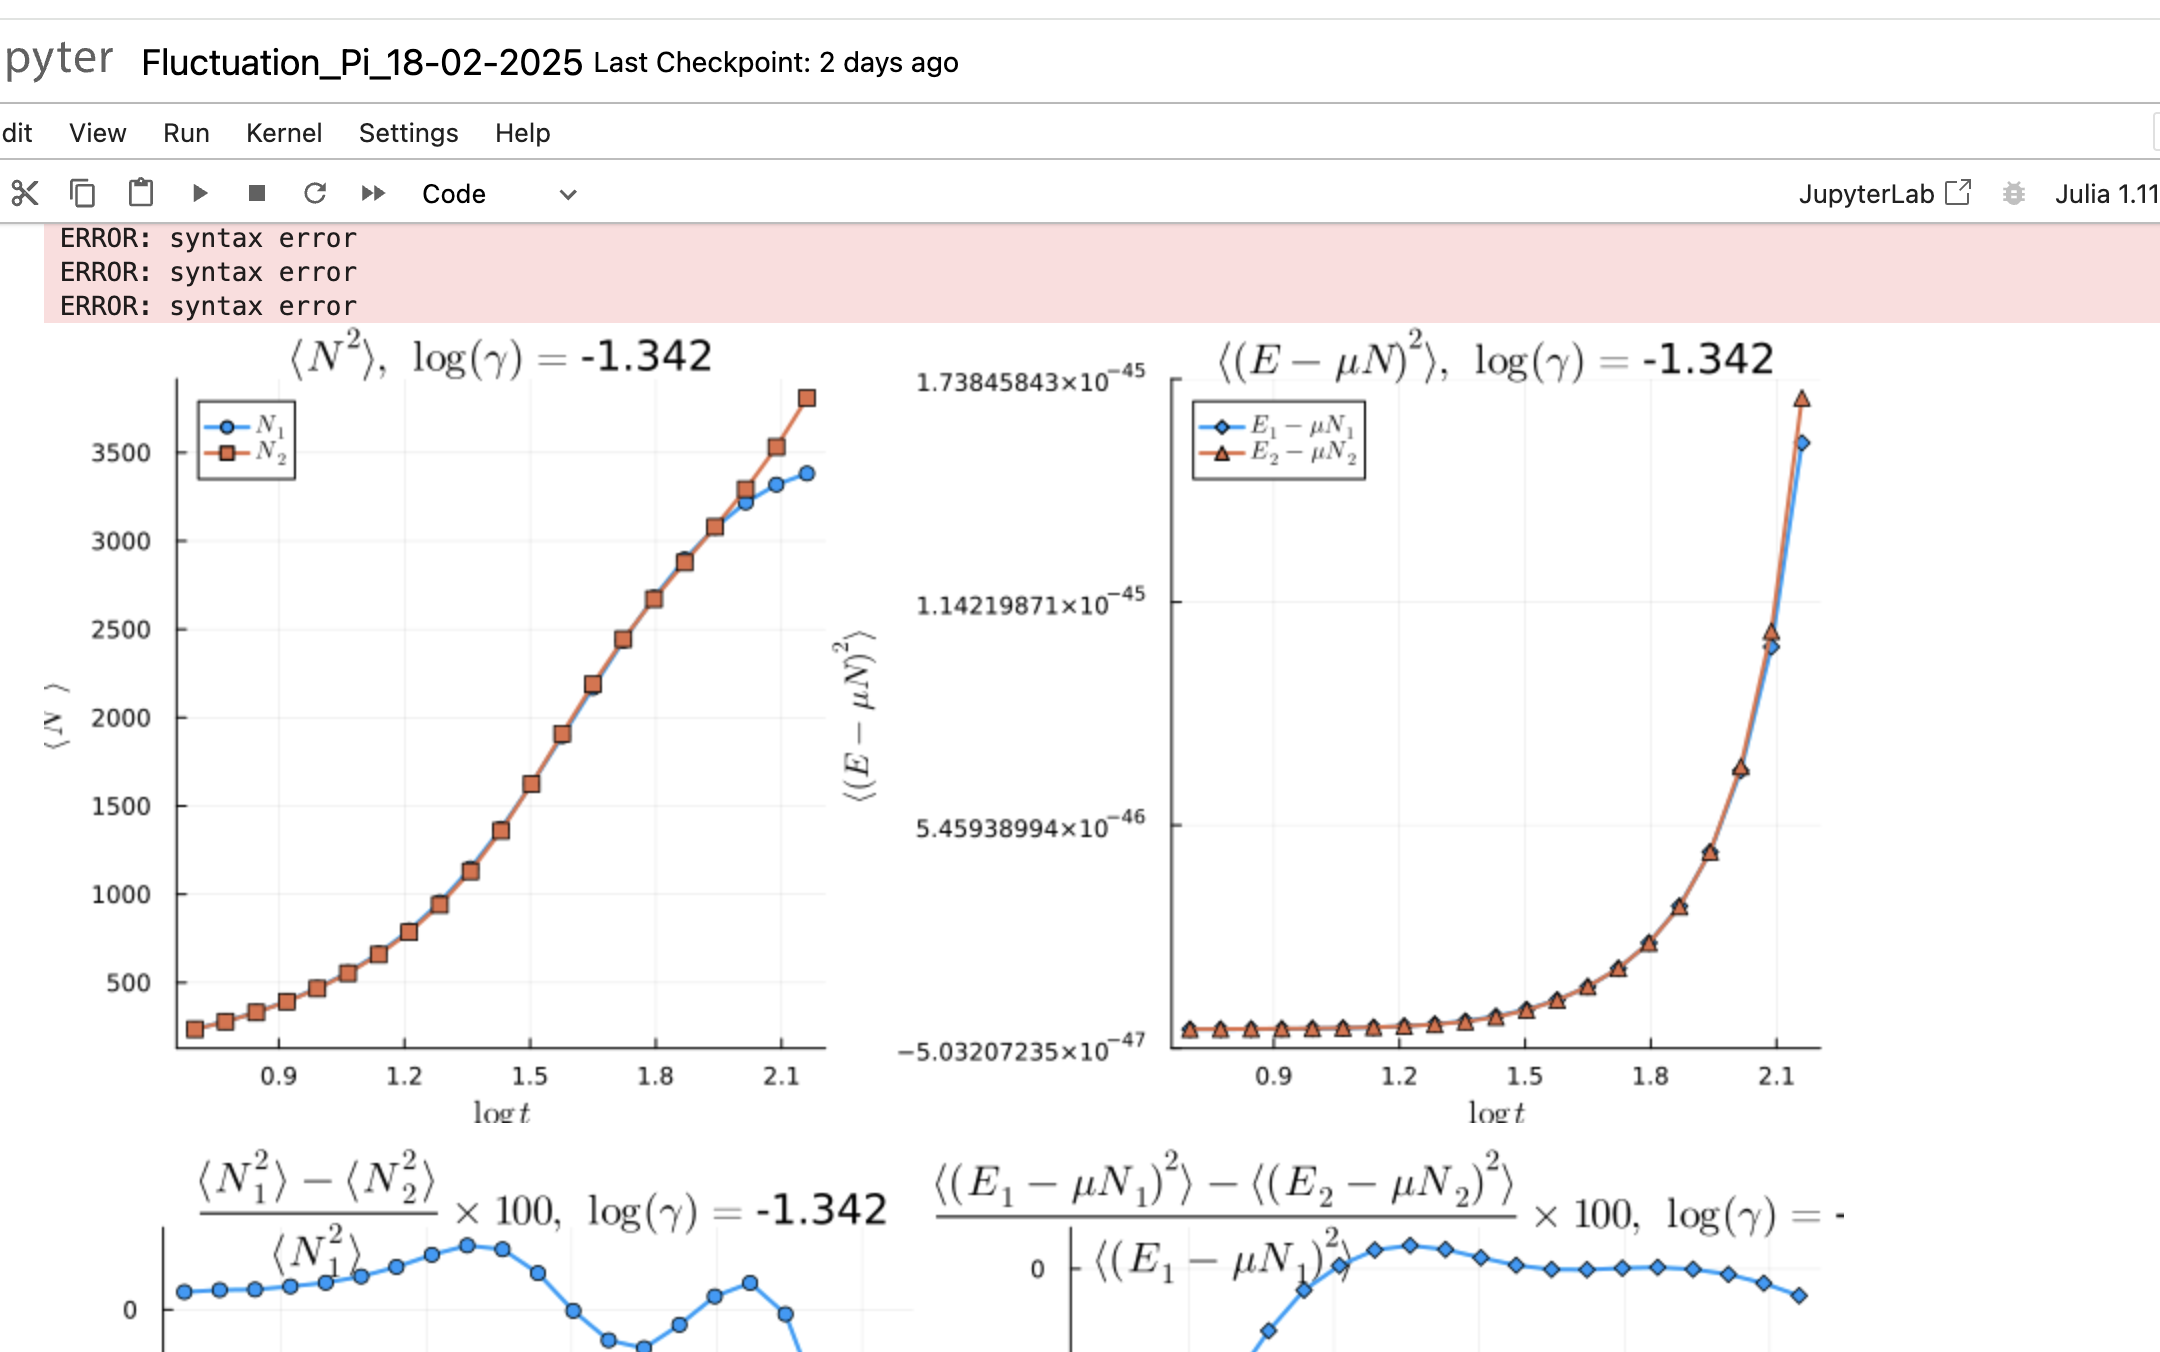
\includegraphics[width=1\textwidth]{Figures/test}

%\begin{aff}
%Donc une a l'ordre un en $\delta \theta (\operator{A}^{(0)})^{-1} %\operator{V}$ 

%\begin{eqnarray*}
%	\langle \delta \Pi ( \theta) \delta \Pi ( \theta') \rangle & = &  ( (\Pi^c_s - \Pi^c)\Pi^c/\Pi^c_s ) ( \theta ) \delta_{\theta, \theta'}/\delta \theta + \mathscr{F}(\theta , \theta' ) ,	
%\end{eqnarray*}

%avec 

%\begin{eqnarray*}
%	\mathscr{F}(\theta , \theta' ) & = & \left [ (\Pi^c_s - \Pi^c )( \theta)  +  (\Pi^c_s - \Pi^c ) ( \theta' )\right ] \frac{\Pi^c}{\Pi^c_s}(\theta)\frac{\Pi^c}{\Pi^c_s}(\theta') \frac{ \Delta( \theta'- \theta )}{ 2 \pi }\\
%	&&  - \left [ (\Pi^c_s - \Pi^c )( \theta)   (\Pi^c_s - \Pi^c ) ( \theta' )\right ] \frac{\Pi^c}{\Pi^c_s}(\theta)\frac{\Pi^c}{\Pi^c_s}(\theta')\int d\theta'' \left (   \frac{ \Pi^c/\Pi^c_s}{\Pi^c_s - \Pi^c} \right )(\theta'') \frac{\Delta(\theta''- \theta)}{2 \pi}\frac{\Delta(\theta''- \theta')}{2 \pi}  	
%\end{eqnarray*}
%\end{aff}



 









\subsection{Exemple : action de $\operator{P}$ sur l’état $\vert \psi_N\rangle$}
%Dans ce chapitre, nous nous intéressons aux fluctuations de la distribution de rapidité \( \delta \rho \) autour d'une distribution de référence \( \rho^c \), qui maximise la contribution à la fonction de partition des états, exprimée comme une fonctionnelle de la distribution \( \rho \) : 

La fonction de partition des états, s'exprime comme une fonctionnelle de la distribution \( \rho \) : 

\begin{eqnarray*}
	\Xi & = & \sum_\rho \exp \left( -\mathcal{A}(\rho) \right).
\end{eqnarray*}  

Dans la section {\em \bf Entropie de Yang-Yang} (\ref{??}), l'action \( \mathcal{A}(\rho) \) s'écrit sous la forme :  

\begin{eqnarray*}
	\mathcal{A}(\rho) & \doteq & - L\mathcal{S}_{YY}(\rho) + L\int f(\theta) \rho (\theta) \, d\theta,		
\end{eqnarray*}  

où \( \mathcal{S}_{YY} \) est la fonctionnelle d'entropie de Yang-Yang, définie dans (\ref{??}), et \( f \) est la fonction paramétrant les charges, introduite dans (\ref{??}).  

Dans cette même section {\em \bf Entropie de Yang-Yang} (\ref{??}), nous avons établi un lien entre \( f \) et distribution de référence \( \rho^c \), qui maximise la contribution à la fonction de partition des états .\\

On veux tester si nos experience est décrit pas un GGE. Pour cela nous nous intéressons aux fluctuations de la distribution de rapidité \( \delta \rho \) autour \( \rho^c \).

%Nous poursuivons à présent avec cette définition de l'action de classe $\mathcal{C}^2$ et admetant une distribution critique $\rho^c$ tel que sa différentielle en ce point critique soit nulle $d\mathcal{A}_{\rho^c} = 0 $ (\ref{??}) de sorte que d'aprés la formule de Taylor-Youg %afin de déterminer les fluctuations autour de \( \Pi^c \). Pour cela, nous réécrivons l'action sous la forme :  

Nous poursuivons à présent avec cette définition de l'action de classe $\mathcal{C}^2$ et admetant une distribution critique $\rho^c$ tel que sa différentielle en ce point critique soit nulle $d\mathcal{A}_{\rho^c} = 0 $ (\ref{??}) de sorte que d'aprés la formule de Taylor-Youg %afin de déterminer les fluctuations autour de \( \Pi^c \). Pour cela, nous réécrivons l'action sous la forme :  

\begin{eqnarray*}  
	\mathcal{A}(\rho^c + \delta \rho) & \underset{ \delta \rho \to 0 }{=} & \mathcal{A}(\rho^c)  + \frac{1}{2} \left. \frac{\delta^2 \mathcal{A}}{\delta \rho^2} \right|_{\rho^c} (\delta \rho) + \mathcal{O}((\delta \rho)^3),  
\end{eqnarray*}  

une expression quadratique pour l'action à l'ordre dominant en \( \delta \Pi \) avec $\left. \frac{\delta^2 \mathcal{A}}{\delta \rho^2} \right|_{\rho^c}$ la forme quadratique définie positive (Fig (\ref{fig.fluctu.A})).

\begin{figure}[H]
	\centering 
	\begin{tikzpicture}
		\begin{scope}[shift={(0,0)}]
			\begin{scope}[transform canvas={scale=0.6}]
				% Définition des couleurs avec les codes HTML
\definecolor{colorOne}{HTML}{443E46}
\definecolor{colorTwo}{HTML}{F6DEB8}
\definecolor{colorThree}{HTML}{908CA4}
\definecolor{colorFour}{HTML}{57659E}
\definecolor{colorFive}{HTML}{C57284}
\definecolor{colorSix}{HTML}{FF5B69}

% Raccourcis pour les couleurs
\def\colorOne{colorOne}
\def\colorTwo{colorTwo}
\def\colorThree{colorThree}
\def\colorFour{colorFour}
\def\colorFive{colorFive}
\def\colorSix{colorSix}

\def\colorslide{blue!50!black}



\begin{scope}
	% Tracer une courbe lisse entre des points
	\draw[shift={(0,0)} ,\colorOne]
		(-1 , 0 ) edge [thick,line width=0.8ex , ->,>=triangle 45  , \colorOne] node [pos = 1 , below ]{\huge$\rho$}( 5  , 0 )
	;
	\draw[shift={(0,0)}, color=\colorOne]
		(0, -1.0 ) edge [thick,line width=0.8ex , ->,>=triangle 45  ]node [pos=0.9,left=0.2cm ]{\huge$\mathcal{A}(\rho)$}( 0  , 5 )
	;
	\draw[]
		(2.5, 0.12 ) edge [thick,line width=0.8ex ,\colorThree ]node [pos=1,below  ]{\huge$\rho^c$} (2.5, -0.12 )	
	;
	
	\draw[]
		(2.5, -0.12 ) edge [thick,line width=0.4ex , dashed, \colorThree ] (2.5, 5.5 )
		(1.5, 1 ) edge [thick,line width=0.4ex , <->,>=triangle 45  , \colorThree ] (3.5, 1 )
		(-0.3,1) edge [thick,line width=0.4ex  , \colorThree ] node [pos=0,left ]{\huge$\mathcal{A}(\rho^c)$} (0.3, 1 )	
	;
    \draw[thick, line width=0.8ex , \colorFour] plot[smooth, tension=0.7] coordinates {
        (1, 5) (1.6 , 3 ) (2.5, 1) (3.5 , 3 )  (4, 5)
    };		
	
\end{scope}

	
			
			\end{scope}
			
			\draw[color = red , scale = 0.5 , draw = none  ] (-2 , -1) rectangle (5, 6) ; 	
		\end{scope}
		
		\begin{scope}[shift={(19,-1)}]
			\begin{scope}[transform canvas={scale=0.6}]
				% Définition des couleurs avec les codes HTML
\definecolor{colorOne}{HTML}{443E46}
\definecolor{colorTwo}{HTML}{F6DEB8}
\definecolor{colorThree}{HTML}{908CA4}
\definecolor{colorFour}{HTML}{57659E}
\definecolor{colorFive}{HTML}{C57284}
\definecolor{colorSix}{HTML}{FF5B69}

% Raccourcis pour les couleurs
\def\colorOne{colorOne}
\def\colorTwo{colorTwo}
\def\colorThree{colorThree}
\def\colorFour{colorFour}
\def\colorFive{colorFive}
\def\colorSix{colorSix}

\def\colorslide{blue!50!black}

\def\Occupation{
	\def\traitx{0.3}
	\def\traity{0.5}
	\draw[shift={(0,0)}]
		(-13.5 , 0 ) edge [thick,line width=0.8ex ]( -3.2  , 0 )
		( -3.2 - \traitx  , 0 - \traity ) edge [thick,line width=0.8ex ]( -3.2 + \traitx  , 0 + \traity  )
		( -2.8 - \traitx  , 0 - \traity ) edge [thick,line width=0.8ex ]( -2.8 + \traitx  , 0 + \traity  )
		(-2.8 , 0 ) edge [thick,line width=0.8ex ](2.8  , 0 )
		( 2.8 - \traitx  , 0 - \traity ) edge [thick,line width=0.8ex ]( 2.8 + \traitx  , 0 + \traity  )
		( 3.2 - \traitx  , 0 - \traity ) edge [thick,line width=0.8ex ]( 3.2 + \traitx  , 0 + \traity  )
		(3.2, 0 ) edge [thick,line width=0.8ex,->,>=triangle 45 , color = black ]node [pos=1.01,below  ]{\huge$\theta$}	( 13  , 0 )
	;
	\draw[shift={(0,0)}, color=\colorOne]
		(-10.5 , -1.5 ) edge [thick,line width=0.8ex , ->,>=triangle 45  ]( -10.5  , 4.5 )
	;
		
	\foreach \r in {1 , ... , 3 } {
%		\draw[
%		decoration={
%		markings,
%    	mark connection node=my node,
%    	mark=at position 0 with{\node [blue,transform shape] (my node) {\large \r};}},
%		color=gray, thick, 
%		line width=0.5ex] decorate { 
%            (-11.0, \r) -- (-10.1, \r )}
%        ;
        \draw[
			color=\colorOne,
			] 
            (-11.0, \r) edge[color=\colorThree , thick,line width=0.5ex] node [pos=-0.5 ]{\large\color{\colorFour} $\frac{\r}{\delta \theta}$ } (-10.3, \r )
        	;
	
	}
	

	
	% Graduation abcsisse 
	% Définitions des listes
% Definitions of the lists
\def\listetuple{-9/\theta_{1}, -8/\theta_{2} , -5/\theta_{3} , -2/\theta_{a-1} , 0/\theta_{a} , 1/\theta_{a+1} , 2/\theta_{a+2} ,  5/\theta_{N-4} , 7/\theta_{N-3},8/\theta_{N-1},9/\theta_{N} }
\def\listetrais{-12 , -11, -10, -9 , -8 , -7 ,  -6 , -5, -4.5,-4, -2 , -1, 0 , 0.5, 1, 2, 4 , 5 ,  6 , 7 , 8 ,8.5, 9 ,  10 , 11, 12 }

% Loop over listetrais
\foreach \r in \listetrais {
    % Initialize found variable to zero
    % Initialize found variable to zero
    %\pgfmathsetmacro\found{0}
    \global\def\found{0}
    \xdef\nomtheta{}
    
    % Check if \r is in listetuple
    \foreach \x/\y in \listetuple { 
        \ifdim \r pt=\x pt % If \r matches any \x in listetuple
            \global\def\found{1} ;
            \xdef\nomtheta{\y} % Set \nomtheta to the corresponding \y
            %\pgfmathsetmacro\found{1} % Set found to 1            
            %\global\pgfmathsetmacro\found{1}
        \fi
    }
    
    %\node [circle, draw, red] (A) at (\r, 2) {\found , $\nomtheta$};
    
    % Draw the line and display \nomtheta if found
    \ifnum\found=1
        \draw[color=\colorOne, thick, line width=0.5ex] 
            (\r, -0.3) -- (\r, 0.3) node[red , pos=-0.5] {\large $\nomtheta$};
         \filldraw[line width=0.5ex, color=\colorSix, outer color=\colorSix, inner color=\colorSix] 
            (\r, 0) circle (4pt);
    \else 
        % Draw without \nomtheta and add a blue circle if not found
        \draw[color=\colorOne, thick, line width=0.5ex] 
            (\r, -0.3) -- (\r, 0.3);
        \filldraw[line width=0.5ex, color=\colorSix, outer color=\colorTwo, inner color=\colorTwo] 
            (\r, 0) circle (4pt); 
    \fi
}

\def\listetrais{-9.5/\theta_{i-1}/2/3, -6.5/\theta_{i}/1/4  ,   -1.5/\theta_{j}/2/4 , 1.5/\theta_{j+1}/-1/3 , 3.5/\theta_{\ell-1}/1/3 , 6.5/\theta_{\ell}/3/4 , 9.5/\theta(\theta_{\ell+1})/-1/3 };



\foreach \r/\nomx/\y/\ys in \listetrais {
	\draw[
		decoration={
		markings,
    	mark connection node=my node,
    	mark=at position .5 with{\node [blue,transform shape] (my node) {\large \color{\colorFour} $\nomx$};}},
		color=\colorThree , thick, 
		line width=0.5ex] decorate { 
            (\r, 0.12) -- (\r, -1.2)}
        ;
     
     \ifdim \y pt > -1 pt 
     	\draw[
			decoration={
			markings,
    		mark connection node=my node,
    		mark=at position .5 with{\node [blue,transform shape] (my node) {\large \color{\colorFour} $\Pi(\nomx) $};}},
			color=\colorThree, thick, 
			line width=0.5ex] decorate { 
            (\r, \y) -- (\r +3, \y)}
        ;
        \draw[
			decoration={
			markings,
    		mark connection node=my node,
    		mark=at position .5 with{\node [blue,transform shape] (my node) {\large \color{\colorFive} $\Pi_s(\nomx) $};}},
			color=\colorFive, thick, 
			line width=0.5ex] decorate { 
            (\r, \ys) -- (\r +3, \ys)}
        ;
     \fi 
     \ifdim \r pt= -1.5 pt
     	\draw[
     		decoration={
			markings,
    		mark connection node=my node,
    		mark=at position .5 with{\node [blue,transform shape] (my node) {\large \color{\colorFour}  $\delta \theta $};},
    		%mark=at position 0.1  with {\arrow[blue, line width=0.5ex]{<}},
    		%mark=at position 1  with {\arrow[blue, line width=0.5ex]{>}}
    		},
        	color=\colorThree,
        	thick,
        	line width=0.5ex,
        	%arrows={Computer Modern Rightarrow[line cap=round]-Computer Modern Rightarrow[line cap=round]}
   			](\r, -1.2) edge[arrows={Computer Modern Rightarrow[line cap=round]-}] (\r + 0.4, -1.2)decorate {
    		(\r, -1.2) -- (\r + 3, -1.2)}(\r + 2, -1.2) edge[arrows={-Computer Modern Rightarrow[line cap=round]}] (\r + 3, -1.2)
    		;
    \fi
			
	
}


			
}


\begin{scope}
	%\draw[help lines , width=1.5ex] (-8,-3) grid (8,3);\draw[help lines ,width=0.5ex , opacity = 0.5] (-3,-3) grid[step=0.1] (3,3));
	
	%\draw[help lines] 
	%	(-3,-3) edge[width=1.5ex] grid (3,3)	
	%	(-3,-3) edge[width=0.5ex , opacity = 0.5] grid (3,3)	
	%;
	\begin{scope}[shift={(0,1)},rotate=0,opacity=1,color=black]
		\Occupation	
		
		%\node[anchor=east, font=\bfseries] at (-11, 0) {\color{red}\large (T = 0 )} ;	
	\end{scope}
	
	
	
	
	\begin{scope}[shift={(-10.5,7)},rotate=0,opacity=1,color=black]
	
	\begin{scope}[shift={(-0,0)},rotate=0,opacity=1,color=black]
	
		\draw[shift={(0,0)} ,line width=1ex,rounded corners = 1ex,color=\colorOne , opacity =1 ,fill=\colorOne!00 , pattern={north east lines} , pattern color=\colorOne!00 ]
			(0 , -1 ) rectangle (5,1)
		;
		

		\begin{scope}[shift={(0.5,0.5)}]
			\draw[color=\colorOne, thick, line width=0.5ex] 
            (0, -0.3) -- (0, 0.3) ;
            \filldraw[line width=0.5ex, color=\colorSix, outer color=\colorSix, inner color=\colorSix] 
            (0, 0) circle (4pt);
            
            \node[anchor=west, font=\bfseries] at (0.2, 0) {\color{\colorSix}\large : quasi-particule};
		\end{scope}
		
		\begin{scope}[shift={(0.5,-0.5)}]
			\draw[color=\colorOne, thick, line width=0.5ex] 
            (0, -0.3) -- (0, 0.3) ;
            \filldraw[line width=0.5ex, color=\colorSix, outer color=\colorTwo, inner color=\colorTwo] 
            (0, 0) circle (4pt);
            
            \node[anchor=west, font=\bfseries] at (0.2, 0) {\color{\colorSix}\large : hole};
		\end{scope}

	\end{scope}
	
	\begin{scope}[shift={(6,0)},rotate=0,opacity=1,color=black]	
		
		\draw[shift={(0,0)} ,line width=1ex,rounded corners = 1ex,color=\colorOne , opacity =1 ,fill=\colorOne!00 , pattern={north east lines} , pattern color=\colorOne!00 ]
			(0 , -1 ) rectangle (7.5,1)
		;
		
		\node[anchor=west] at (0.5, 0.5) {\color{\colorFour}\large $\Pi$ };\node[anchor=west, font=\bfseries] at (1, 0.5) {\color{\colorFour}\large : quasi-particule distribution};
		
		\node[anchor=west] at (0.5, -0.5) {\color{\colorFour}\large $\Pi_h$ };\node[anchor=west, font=\bfseries] at (1, -0.5) {\color{\colorFour}\large  : hole distribution};
		
	\end{scope}
	
	\begin{scope}[shift={(14.5,0)},rotate=0,opacity=1,color=black]	
		
		\draw[shift={(0,0)} ,line width=1ex,rounded corners = 1ex,color=\colorOne , opacity =1 ,fill=\colorOne!00 , pattern={north east lines} , pattern color=\colorOne!00 ]
			(0 , -0.5 ) rectangle (7.0,0.5)
		;
		
		\node[anchor=west] at (0.2, 0) {\color{\colorFour}\large ${\color{\colorFive}\Pi_s} = \Pi + \Pi_h $ } node[anchor=west , font=\bfseries] at (3.1 , 0 )  {\color{\colorFour}\large {\color{\colorFive} : density of states}};
		
	\end{scope}
	
	
	\end{scope}


		
	
\end{scope}

	
			
			\end{scope}
			\begin{scope}[scale=1]
				\draw[color = red , scale = 1 , draw = none  ] (-1 , -1) rectangle (5, 5) ; 
			\end{scope}	
		\end{scope}

		
				
			
	\end{tikzpicture}	
	\captionsetup{skip=10pt} % Ajoute de l’espace après la légende
	\label{fig.fluctu.A}
\end{figure}


On discrétise l'axe des rapidités en  petite cellule de rapidité $[\theta, \theta+\delta\theta]$, qui contient $L\rho(\theta) \delta \theta$ rapidités. 
	



Avec ces petites tranches, la forme quadratique s’écrit :

\begin{eqnarray*}
    \left. \frac{\delta^2 \mathcal{A}}{{\delta \rho}^2} \right|_{\rho^c}(\delta \rho ) &=&  \sum_{a,b \mid \text{tranche}}  
    \delta \rho(\theta_a)  \frac{\partial^2 \mathcal{A}}{\partial \delta \rho(\theta_a) \partial \delta \rho(\theta_b) } (\rho^c)  \delta \rho(\theta_b).
\end{eqnarray*}
Les fluctuations s’écrivent donc :

\begin{eqnarray*}
    \langle \delta \rho ( \theta) \delta \rho ( \theta') \rangle &=&  
    \frac{ \int d\delta \rho \, \delta \rho(\theta) \delta \rho ( \theta') 
    \exp \left( - \frac{1}{2} \sum_{a,b \mid \text{tranche}}  
    \delta \rho(\theta_a) \frac{\partial^2 \mathcal{A}}{\partial \delta \rho(\theta_a) \partial \delta \rho(\theta_b) } (\rho^c)  \delta \rho(\theta_b) \right) }
    { \int d\delta \Pi  
    \exp \left( - \frac{1}{2} \sum_{a,b \mid \text{tranche}}  
    \delta \rho(\theta_a) \frac{\partial^2 \mathcal{A}}{\partial \delta \rho(\theta_a) \partial \delta \rho(\theta_b) } (\rho^c)  \delta \rho(\theta_b) \right) } \\
    &=& \left( \mathbf{A}^{-1} \right)_{\theta , \theta'}
\end{eqnarray*}


\begin{aff}

\begin{eqnarray*}
	\langle \delta \rho ( \theta) \delta \rho ( \theta') \rangle &=& 	\left( \mathbf{A}^{-1} \right)_{\theta , \theta'}
\end{eqnarray*}

	
avec la  {\em matrice hessienne} $\mathbf{A}_{\theta , \theta'} \equiv \frac{\partial^2 \mathcal{A}}{\partial \delta \rho(\theta) \partial \delta \rho(\theta') }(\rho^c)$, au point critique/ qui maximise la probabilité  $\rho^c=\rho^c_s \nu^c $, s'écrit

\begin{eqnarray*}
	\operator{A} & = & \operator{A}^{(0)} + \delta \theta \operator{V}
\end{eqnarray*}

avec 

\begin{eqnarray*}
	A^{(0)}_{\theta , \theta'}  & = &  L\delta \theta \left ( \frac{ 1}{\rho^c_s ( 1  - \nu^c ) \nu^c } \right )(\theta)    \delta({\theta - \theta '})	,\\
	V_{\theta , \theta'}  &= & L \delta \theta \left \{ - \left [ \left ( \frac{1}{\rho^c_s( 1 - \nu^c) } \right ) ( \theta)  +  \left ( \frac{1}{\rho^c_s( 1 - \nu^c) } \right ) ( \theta' )\right ] \frac{ \Delta( \theta'- \theta )}{ 2 \pi } + \int d\theta''  \left ( \frac{\nu^c}{\rho^c_s( 1 - \nu^c) } \right )(\theta'') \frac{\Delta(\theta''- \theta)}{2 \pi}\frac{\Delta(\theta''- \theta')}{2 \pi}   \right \} 	
\end{eqnarray*}

\end{aff}

\subsection{Testes}

\begin{eqnarray*}
	\Delta_{\operator{\mathcal{N}}}^2  & = &  \frac{1}{\beta} \left . \frac{\partial \langle \operator{\mathcal{N}} \rangle}{\partial \mu} \right )_T \\
	\Delta_{\operator{\mathcal{E}}-\mu \operator{\mathcal{N}}}^2  & = &  - \left . \frac{\partial \langle \operator{\mathcal{E}}-\mu \operator{\mathcal{N}} \rangle}{\partial \beta} \right )_\mu 
\end{eqnarray*}

et 

\begin{eqnarray*}
	\Delta_{\operator{\mathcal{N}}}^2  &= & L^2 \int d\theta_a \int d \theta_b \, \langle \delta \rho(\theta_a) \delta \rho(\theta_b) \rangle \\
	\Delta_{\operator{\mathcal{E}}-\mu \operator{\mathcal{N}}}^2  & = & L^2 \int d\theta_a \int d \theta_b \, \left ( - \mu + \frac{1}2 m \theta_a^2  \right  )\left ( - \mu + \frac{1}2 m \theta_b^2  \right  )  \langle \delta \rho(\theta_a) \delta \rho(\theta_b) \rangle
\end{eqnarray*}

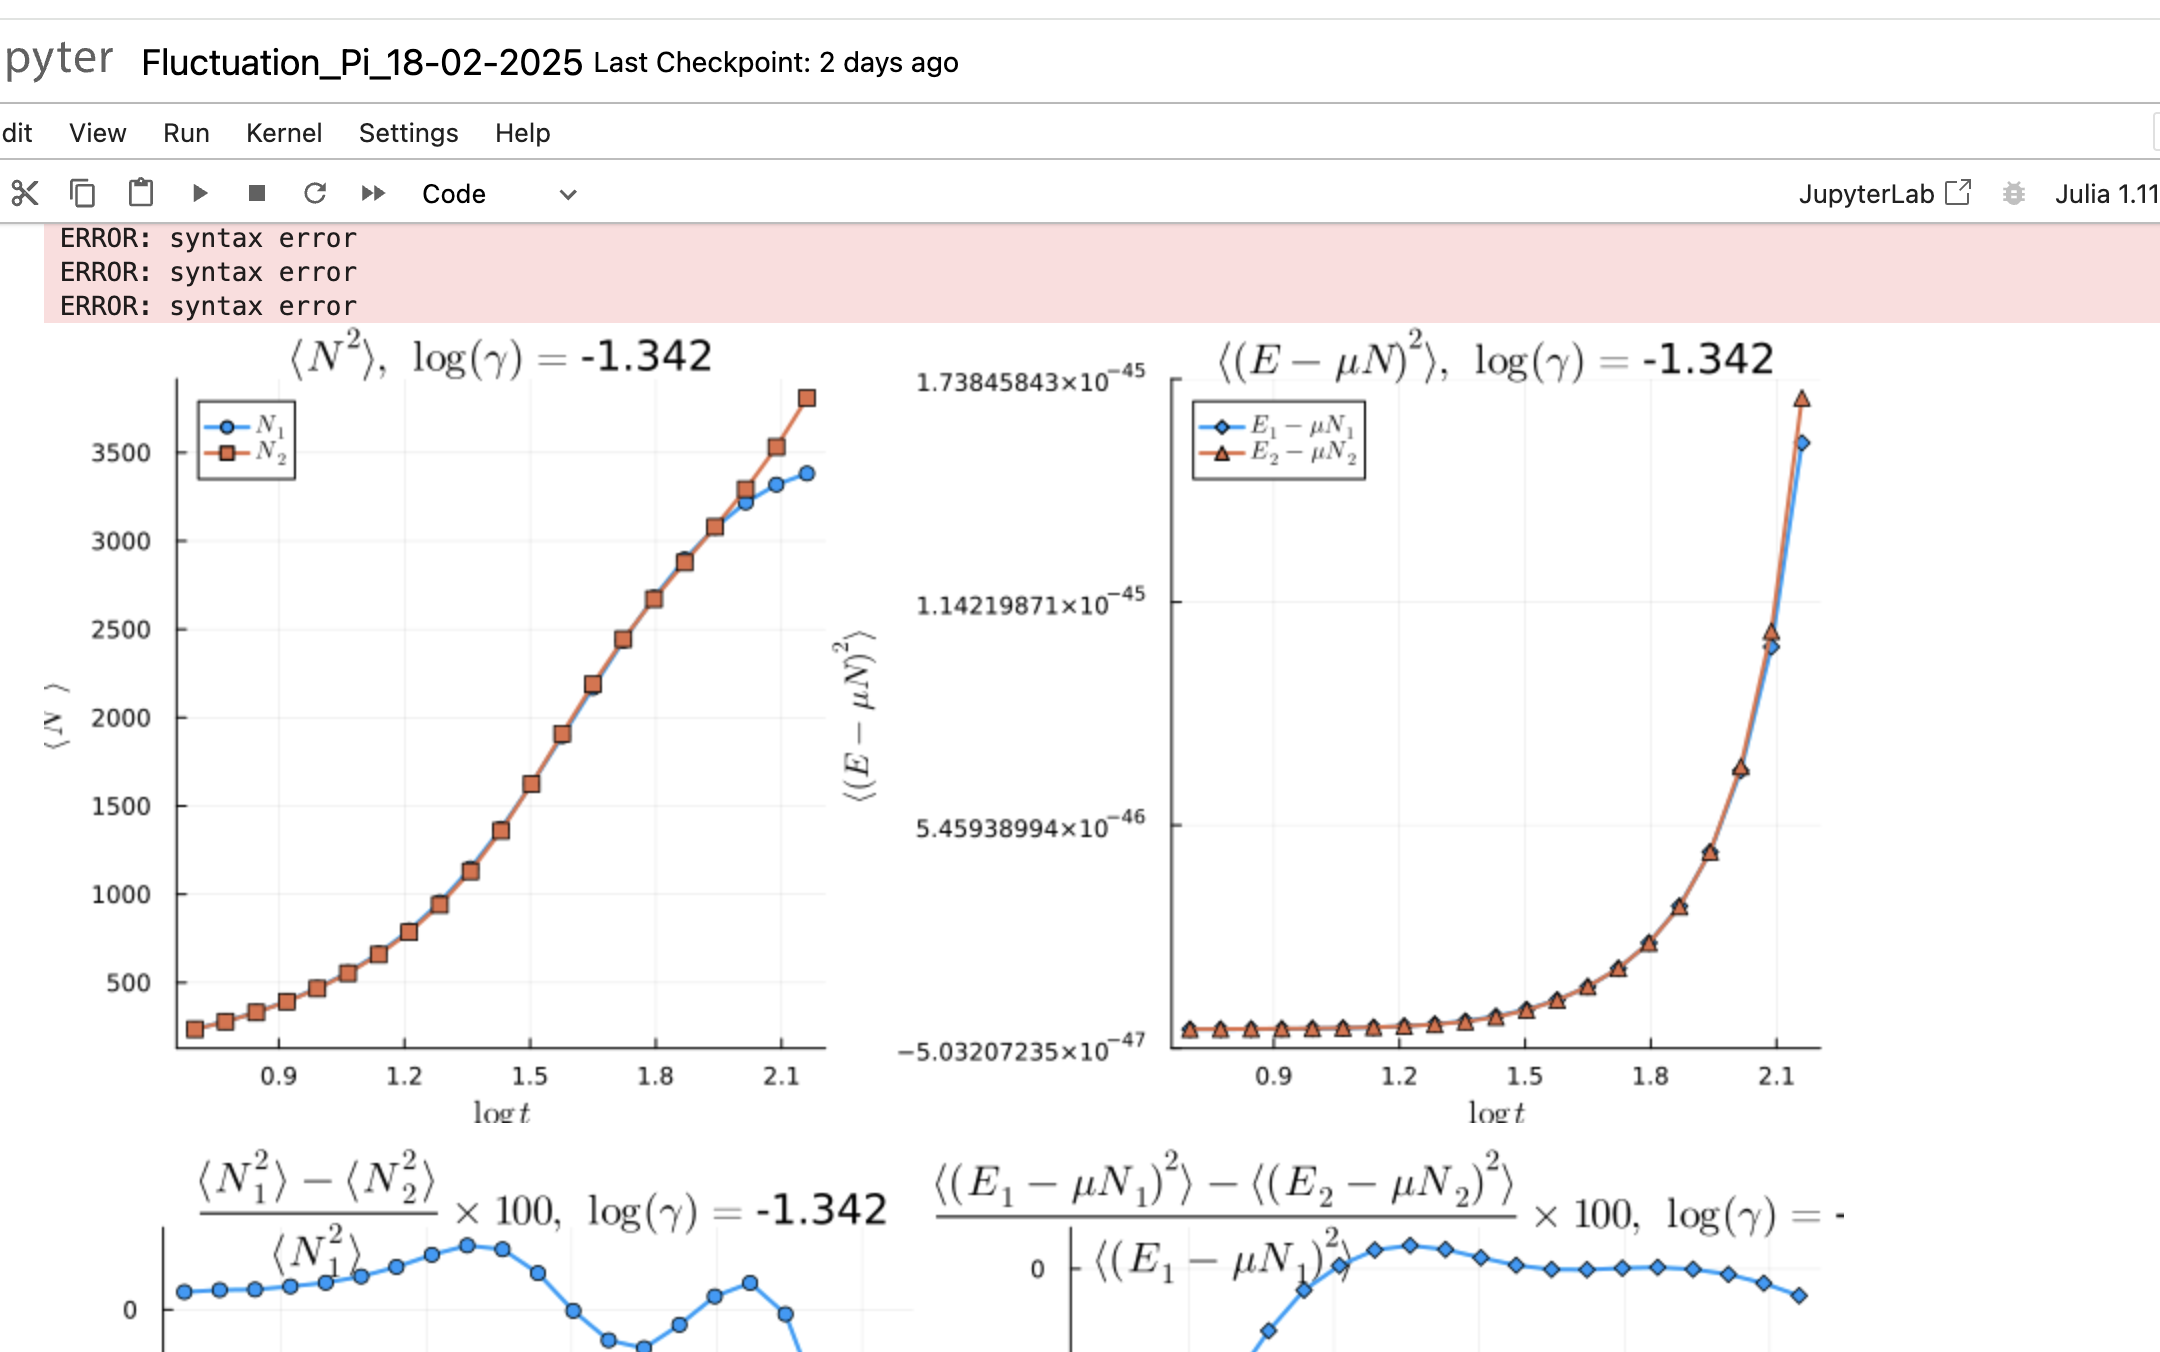
\includegraphics[width=1\textwidth]{Figures/test}

%\begin{aff}
%Donc une a l'ordre un en $\delta \theta (\operator{A}^{(0)})^{-1} %\operator{V}$ 

%\begin{eqnarray*}
%	\langle \delta \Pi ( \theta) \delta \Pi ( \theta') \rangle & = &  ( (\Pi^c_s - \Pi^c)\Pi^c/\Pi^c_s ) ( \theta ) \delta_{\theta, \theta'}/\delta \theta + \mathscr{F}(\theta , \theta' ) ,	
%\end{eqnarray*}

%avec 

%\begin{eqnarray*}
%	\mathscr{F}(\theta , \theta' ) & = & \left [ (\Pi^c_s - \Pi^c )( \theta)  +  (\Pi^c_s - \Pi^c ) ( \theta' )\right ] \frac{\Pi^c}{\Pi^c_s}(\theta)\frac{\Pi^c}{\Pi^c_s}(\theta') \frac{ \Delta( \theta'- \theta )}{ 2 \pi }\\
%	&&  - \left [ (\Pi^c_s - \Pi^c )( \theta)   (\Pi^c_s - \Pi^c ) ( \theta' )\right ] \frac{\Pi^c}{\Pi^c_s}(\theta)\frac{\Pi^c}{\Pi^c_s}(\theta')\int d\theta'' \left (   \frac{ \Pi^c/\Pi^c_s}{\Pi^c_s - \Pi^c} \right )(\theta'') \frac{\Delta(\theta''- \theta)}{2 \pi}\frac{\Delta(\theta''- \theta')}{2 \pi}  	
%\end{eqnarray*}
%\end{aff}



 









\subsection{Aaction de $\operator{H}$ sur l’état $\vert \psi_N\rangle$}
%Dans ce chapitre, nous nous intéressons aux fluctuations de la distribution de rapidité \( \delta \rho \) autour d'une distribution de référence \( \rho^c \), qui maximise la contribution à la fonction de partition des états, exprimée comme une fonctionnelle de la distribution \( \rho \) : 

La fonction de partition des états, s'exprime comme une fonctionnelle de la distribution \( \rho \) : 

\begin{eqnarray*}
	\Xi & = & \sum_\rho \exp \left( -\mathcal{A}(\rho) \right).
\end{eqnarray*}  

Dans la section {\em \bf Entropie de Yang-Yang} (\ref{??}), l'action \( \mathcal{A}(\rho) \) s'écrit sous la forme :  

\begin{eqnarray*}
	\mathcal{A}(\rho) & \doteq & - L\mathcal{S}_{YY}(\rho) + L\int f(\theta) \rho (\theta) \, d\theta,		
\end{eqnarray*}  

où \( \mathcal{S}_{YY} \) est la fonctionnelle d'entropie de Yang-Yang, définie dans (\ref{??}), et \( f \) est la fonction paramétrant les charges, introduite dans (\ref{??}).  

Dans cette même section {\em \bf Entropie de Yang-Yang} (\ref{??}), nous avons établi un lien entre \( f \) et distribution de référence \( \rho^c \), qui maximise la contribution à la fonction de partition des états .\\

On veux tester si nos experience est décrit pas un GGE. Pour cela nous nous intéressons aux fluctuations de la distribution de rapidité \( \delta \rho \) autour \( \rho^c \).

%Nous poursuivons à présent avec cette définition de l'action de classe $\mathcal{C}^2$ et admetant une distribution critique $\rho^c$ tel que sa différentielle en ce point critique soit nulle $d\mathcal{A}_{\rho^c} = 0 $ (\ref{??}) de sorte que d'aprés la formule de Taylor-Youg %afin de déterminer les fluctuations autour de \( \Pi^c \). Pour cela, nous réécrivons l'action sous la forme :  

Nous poursuivons à présent avec cette définition de l'action de classe $\mathcal{C}^2$ et admetant une distribution critique $\rho^c$ tel que sa différentielle en ce point critique soit nulle $d\mathcal{A}_{\rho^c} = 0 $ (\ref{??}) de sorte que d'aprés la formule de Taylor-Youg %afin de déterminer les fluctuations autour de \( \Pi^c \). Pour cela, nous réécrivons l'action sous la forme :  

\begin{eqnarray*}  
	\mathcal{A}(\rho^c + \delta \rho) & \underset{ \delta \rho \to 0 }{=} & \mathcal{A}(\rho^c)  + \frac{1}{2} \left. \frac{\delta^2 \mathcal{A}}{\delta \rho^2} \right|_{\rho^c} (\delta \rho) + \mathcal{O}((\delta \rho)^3),  
\end{eqnarray*}  

une expression quadratique pour l'action à l'ordre dominant en \( \delta \Pi \) avec $\left. \frac{\delta^2 \mathcal{A}}{\delta \rho^2} \right|_{\rho^c}$ la forme quadratique définie positive (Fig (\ref{fig.fluctu.A})).

\begin{figure}[H]
	\centering 
	\begin{tikzpicture}
		\begin{scope}[shift={(0,0)}]
			\begin{scope}[transform canvas={scale=0.6}]
				% Définition des couleurs avec les codes HTML
\definecolor{colorOne}{HTML}{443E46}
\definecolor{colorTwo}{HTML}{F6DEB8}
\definecolor{colorThree}{HTML}{908CA4}
\definecolor{colorFour}{HTML}{57659E}
\definecolor{colorFive}{HTML}{C57284}
\definecolor{colorSix}{HTML}{FF5B69}

% Raccourcis pour les couleurs
\def\colorOne{colorOne}
\def\colorTwo{colorTwo}
\def\colorThree{colorThree}
\def\colorFour{colorFour}
\def\colorFive{colorFive}
\def\colorSix{colorSix}

\def\colorslide{blue!50!black}



\begin{scope}
	% Tracer une courbe lisse entre des points
	\draw[shift={(0,0)} ,\colorOne]
		(-1 , 0 ) edge [thick,line width=0.8ex , ->,>=triangle 45  , \colorOne] node [pos = 1 , below ]{\huge$\rho$}( 5  , 0 )
	;
	\draw[shift={(0,0)}, color=\colorOne]
		(0, -1.0 ) edge [thick,line width=0.8ex , ->,>=triangle 45  ]node [pos=0.9,left=0.2cm ]{\huge$\mathcal{A}(\rho)$}( 0  , 5 )
	;
	\draw[]
		(2.5, 0.12 ) edge [thick,line width=0.8ex ,\colorThree ]node [pos=1,below  ]{\huge$\rho^c$} (2.5, -0.12 )	
	;
	
	\draw[]
		(2.5, -0.12 ) edge [thick,line width=0.4ex , dashed, \colorThree ] (2.5, 5.5 )
		(1.5, 1 ) edge [thick,line width=0.4ex , <->,>=triangle 45  , \colorThree ] (3.5, 1 )
		(-0.3,1) edge [thick,line width=0.4ex  , \colorThree ] node [pos=0,left ]{\huge$\mathcal{A}(\rho^c)$} (0.3, 1 )	
	;
    \draw[thick, line width=0.8ex , \colorFour] plot[smooth, tension=0.7] coordinates {
        (1, 5) (1.6 , 3 ) (2.5, 1) (3.5 , 3 )  (4, 5)
    };		
	
\end{scope}

	
			
			\end{scope}
			
			\draw[color = red , scale = 0.5 , draw = none  ] (-2 , -1) rectangle (5, 6) ; 	
		\end{scope}
		
		\begin{scope}[shift={(19,-1)}]
			\begin{scope}[transform canvas={scale=0.6}]
				% Définition des couleurs avec les codes HTML
\definecolor{colorOne}{HTML}{443E46}
\definecolor{colorTwo}{HTML}{F6DEB8}
\definecolor{colorThree}{HTML}{908CA4}
\definecolor{colorFour}{HTML}{57659E}
\definecolor{colorFive}{HTML}{C57284}
\definecolor{colorSix}{HTML}{FF5B69}

% Raccourcis pour les couleurs
\def\colorOne{colorOne}
\def\colorTwo{colorTwo}
\def\colorThree{colorThree}
\def\colorFour{colorFour}
\def\colorFive{colorFive}
\def\colorSix{colorSix}

\def\colorslide{blue!50!black}

\def\Occupation{
	\def\traitx{0.3}
	\def\traity{0.5}
	\draw[shift={(0,0)}]
		(-13.5 , 0 ) edge [thick,line width=0.8ex ]( -3.2  , 0 )
		( -3.2 - \traitx  , 0 - \traity ) edge [thick,line width=0.8ex ]( -3.2 + \traitx  , 0 + \traity  )
		( -2.8 - \traitx  , 0 - \traity ) edge [thick,line width=0.8ex ]( -2.8 + \traitx  , 0 + \traity  )
		(-2.8 , 0 ) edge [thick,line width=0.8ex ](2.8  , 0 )
		( 2.8 - \traitx  , 0 - \traity ) edge [thick,line width=0.8ex ]( 2.8 + \traitx  , 0 + \traity  )
		( 3.2 - \traitx  , 0 - \traity ) edge [thick,line width=0.8ex ]( 3.2 + \traitx  , 0 + \traity  )
		(3.2, 0 ) edge [thick,line width=0.8ex,->,>=triangle 45 , color = black ]node [pos=1.01,below  ]{\huge$\theta$}	( 13  , 0 )
	;
	\draw[shift={(0,0)}, color=\colorOne]
		(-10.5 , -1.5 ) edge [thick,line width=0.8ex , ->,>=triangle 45  ]( -10.5  , 4.5 )
	;
		
	\foreach \r in {1 , ... , 3 } {
%		\draw[
%		decoration={
%		markings,
%    	mark connection node=my node,
%    	mark=at position 0 with{\node [blue,transform shape] (my node) {\large \r};}},
%		color=gray, thick, 
%		line width=0.5ex] decorate { 
%            (-11.0, \r) -- (-10.1, \r )}
%        ;
        \draw[
			color=\colorOne,
			] 
            (-11.0, \r) edge[color=\colorThree , thick,line width=0.5ex] node [pos=-0.5 ]{\large\color{\colorFour} $\frac{\r}{\delta \theta}$ } (-10.3, \r )
        	;
	
	}
	

	
	% Graduation abcsisse 
	% Définitions des listes
% Definitions of the lists
\def\listetuple{-9/\theta_{1}, -8/\theta_{2} , -5/\theta_{3} , -2/\theta_{a-1} , 0/\theta_{a} , 1/\theta_{a+1} , 2/\theta_{a+2} ,  5/\theta_{N-4} , 7/\theta_{N-3},8/\theta_{N-1},9/\theta_{N} }
\def\listetrais{-12 , -11, -10, -9 , -8 , -7 ,  -6 , -5, -4.5,-4, -2 , -1, 0 , 0.5, 1, 2, 4 , 5 ,  6 , 7 , 8 ,8.5, 9 ,  10 , 11, 12 }

% Loop over listetrais
\foreach \r in \listetrais {
    % Initialize found variable to zero
    % Initialize found variable to zero
    %\pgfmathsetmacro\found{0}
    \global\def\found{0}
    \xdef\nomtheta{}
    
    % Check if \r is in listetuple
    \foreach \x/\y in \listetuple { 
        \ifdim \r pt=\x pt % If \r matches any \x in listetuple
            \global\def\found{1} ;
            \xdef\nomtheta{\y} % Set \nomtheta to the corresponding \y
            %\pgfmathsetmacro\found{1} % Set found to 1            
            %\global\pgfmathsetmacro\found{1}
        \fi
    }
    
    %\node [circle, draw, red] (A) at (\r, 2) {\found , $\nomtheta$};
    
    % Draw the line and display \nomtheta if found
    \ifnum\found=1
        \draw[color=\colorOne, thick, line width=0.5ex] 
            (\r, -0.3) -- (\r, 0.3) node[red , pos=-0.5] {\large $\nomtheta$};
         \filldraw[line width=0.5ex, color=\colorSix, outer color=\colorSix, inner color=\colorSix] 
            (\r, 0) circle (4pt);
    \else 
        % Draw without \nomtheta and add a blue circle if not found
        \draw[color=\colorOne, thick, line width=0.5ex] 
            (\r, -0.3) -- (\r, 0.3);
        \filldraw[line width=0.5ex, color=\colorSix, outer color=\colorTwo, inner color=\colorTwo] 
            (\r, 0) circle (4pt); 
    \fi
}

\def\listetrais{-9.5/\theta_{i-1}/2/3, -6.5/\theta_{i}/1/4  ,   -1.5/\theta_{j}/2/4 , 1.5/\theta_{j+1}/-1/3 , 3.5/\theta_{\ell-1}/1/3 , 6.5/\theta_{\ell}/3/4 , 9.5/\theta(\theta_{\ell+1})/-1/3 };



\foreach \r/\nomx/\y/\ys in \listetrais {
	\draw[
		decoration={
		markings,
    	mark connection node=my node,
    	mark=at position .5 with{\node [blue,transform shape] (my node) {\large \color{\colorFour} $\nomx$};}},
		color=\colorThree , thick, 
		line width=0.5ex] decorate { 
            (\r, 0.12) -- (\r, -1.2)}
        ;
     
     \ifdim \y pt > -1 pt 
     	\draw[
			decoration={
			markings,
    		mark connection node=my node,
    		mark=at position .5 with{\node [blue,transform shape] (my node) {\large \color{\colorFour} $\Pi(\nomx) $};}},
			color=\colorThree, thick, 
			line width=0.5ex] decorate { 
            (\r, \y) -- (\r +3, \y)}
        ;
        \draw[
			decoration={
			markings,
    		mark connection node=my node,
    		mark=at position .5 with{\node [blue,transform shape] (my node) {\large \color{\colorFive} $\Pi_s(\nomx) $};}},
			color=\colorFive, thick, 
			line width=0.5ex] decorate { 
            (\r, \ys) -- (\r +3, \ys)}
        ;
     \fi 
     \ifdim \r pt= -1.5 pt
     	\draw[
     		decoration={
			markings,
    		mark connection node=my node,
    		mark=at position .5 with{\node [blue,transform shape] (my node) {\large \color{\colorFour}  $\delta \theta $};},
    		%mark=at position 0.1  with {\arrow[blue, line width=0.5ex]{<}},
    		%mark=at position 1  with {\arrow[blue, line width=0.5ex]{>}}
    		},
        	color=\colorThree,
        	thick,
        	line width=0.5ex,
        	%arrows={Computer Modern Rightarrow[line cap=round]-Computer Modern Rightarrow[line cap=round]}
   			](\r, -1.2) edge[arrows={Computer Modern Rightarrow[line cap=round]-}] (\r + 0.4, -1.2)decorate {
    		(\r, -1.2) -- (\r + 3, -1.2)}(\r + 2, -1.2) edge[arrows={-Computer Modern Rightarrow[line cap=round]}] (\r + 3, -1.2)
    		;
    \fi
			
	
}


			
}


\begin{scope}
	%\draw[help lines , width=1.5ex] (-8,-3) grid (8,3);\draw[help lines ,width=0.5ex , opacity = 0.5] (-3,-3) grid[step=0.1] (3,3));
	
	%\draw[help lines] 
	%	(-3,-3) edge[width=1.5ex] grid (3,3)	
	%	(-3,-3) edge[width=0.5ex , opacity = 0.5] grid (3,3)	
	%;
	\begin{scope}[shift={(0,1)},rotate=0,opacity=1,color=black]
		\Occupation	
		
		%\node[anchor=east, font=\bfseries] at (-11, 0) {\color{red}\large (T = 0 )} ;	
	\end{scope}
	
	
	
	
	\begin{scope}[shift={(-10.5,7)},rotate=0,opacity=1,color=black]
	
	\begin{scope}[shift={(-0,0)},rotate=0,opacity=1,color=black]
	
		\draw[shift={(0,0)} ,line width=1ex,rounded corners = 1ex,color=\colorOne , opacity =1 ,fill=\colorOne!00 , pattern={north east lines} , pattern color=\colorOne!00 ]
			(0 , -1 ) rectangle (5,1)
		;
		

		\begin{scope}[shift={(0.5,0.5)}]
			\draw[color=\colorOne, thick, line width=0.5ex] 
            (0, -0.3) -- (0, 0.3) ;
            \filldraw[line width=0.5ex, color=\colorSix, outer color=\colorSix, inner color=\colorSix] 
            (0, 0) circle (4pt);
            
            \node[anchor=west, font=\bfseries] at (0.2, 0) {\color{\colorSix}\large : quasi-particule};
		\end{scope}
		
		\begin{scope}[shift={(0.5,-0.5)}]
			\draw[color=\colorOne, thick, line width=0.5ex] 
            (0, -0.3) -- (0, 0.3) ;
            \filldraw[line width=0.5ex, color=\colorSix, outer color=\colorTwo, inner color=\colorTwo] 
            (0, 0) circle (4pt);
            
            \node[anchor=west, font=\bfseries] at (0.2, 0) {\color{\colorSix}\large : hole};
		\end{scope}

	\end{scope}
	
	\begin{scope}[shift={(6,0)},rotate=0,opacity=1,color=black]	
		
		\draw[shift={(0,0)} ,line width=1ex,rounded corners = 1ex,color=\colorOne , opacity =1 ,fill=\colorOne!00 , pattern={north east lines} , pattern color=\colorOne!00 ]
			(0 , -1 ) rectangle (7.5,1)
		;
		
		\node[anchor=west] at (0.5, 0.5) {\color{\colorFour}\large $\Pi$ };\node[anchor=west, font=\bfseries] at (1, 0.5) {\color{\colorFour}\large : quasi-particule distribution};
		
		\node[anchor=west] at (0.5, -0.5) {\color{\colorFour}\large $\Pi_h$ };\node[anchor=west, font=\bfseries] at (1, -0.5) {\color{\colorFour}\large  : hole distribution};
		
	\end{scope}
	
	\begin{scope}[shift={(14.5,0)},rotate=0,opacity=1,color=black]	
		
		\draw[shift={(0,0)} ,line width=1ex,rounded corners = 1ex,color=\colorOne , opacity =1 ,fill=\colorOne!00 , pattern={north east lines} , pattern color=\colorOne!00 ]
			(0 , -0.5 ) rectangle (7.0,0.5)
		;
		
		\node[anchor=west] at (0.2, 0) {\color{\colorFour}\large ${\color{\colorFive}\Pi_s} = \Pi + \Pi_h $ } node[anchor=west , font=\bfseries] at (3.1 , 0 )  {\color{\colorFour}\large {\color{\colorFive} : density of states}};
		
	\end{scope}
	
	
	\end{scope}


		
	
\end{scope}

	
			
			\end{scope}
			\begin{scope}[scale=1]
				\draw[color = red , scale = 1 , draw = none  ] (-1 , -1) rectangle (5, 5) ; 
			\end{scope}	
		\end{scope}

		
				
			
	\end{tikzpicture}	
	\captionsetup{skip=10pt} % Ajoute de l’espace après la légende
	\label{fig.fluctu.A}
\end{figure}


On discrétise l'axe des rapidités en  petite cellule de rapidité $[\theta, \theta+\delta\theta]$, qui contient $L\rho(\theta) \delta \theta$ rapidités. 
	



Avec ces petites tranches, la forme quadratique s’écrit :

\begin{eqnarray*}
    \left. \frac{\delta^2 \mathcal{A}}{{\delta \rho}^2} \right|_{\rho^c}(\delta \rho ) &=&  \sum_{a,b \mid \text{tranche}}  
    \delta \rho(\theta_a)  \frac{\partial^2 \mathcal{A}}{\partial \delta \rho(\theta_a) \partial \delta \rho(\theta_b) } (\rho^c)  \delta \rho(\theta_b).
\end{eqnarray*}
Les fluctuations s’écrivent donc :

\begin{eqnarray*}
    \langle \delta \rho ( \theta) \delta \rho ( \theta') \rangle &=&  
    \frac{ \int d\delta \rho \, \delta \rho(\theta) \delta \rho ( \theta') 
    \exp \left( - \frac{1}{2} \sum_{a,b \mid \text{tranche}}  
    \delta \rho(\theta_a) \frac{\partial^2 \mathcal{A}}{\partial \delta \rho(\theta_a) \partial \delta \rho(\theta_b) } (\rho^c)  \delta \rho(\theta_b) \right) }
    { \int d\delta \Pi  
    \exp \left( - \frac{1}{2} \sum_{a,b \mid \text{tranche}}  
    \delta \rho(\theta_a) \frac{\partial^2 \mathcal{A}}{\partial \delta \rho(\theta_a) \partial \delta \rho(\theta_b) } (\rho^c)  \delta \rho(\theta_b) \right) } \\
    &=& \left( \mathbf{A}^{-1} \right)_{\theta , \theta'}
\end{eqnarray*}


\begin{aff}

\begin{eqnarray*}
	\langle \delta \rho ( \theta) \delta \rho ( \theta') \rangle &=& 	\left( \mathbf{A}^{-1} \right)_{\theta , \theta'}
\end{eqnarray*}

	
avec la  {\em matrice hessienne} $\mathbf{A}_{\theta , \theta'} \equiv \frac{\partial^2 \mathcal{A}}{\partial \delta \rho(\theta) \partial \delta \rho(\theta') }(\rho^c)$, au point critique/ qui maximise la probabilité  $\rho^c=\rho^c_s \nu^c $, s'écrit

\begin{eqnarray*}
	\operator{A} & = & \operator{A}^{(0)} + \delta \theta \operator{V}
\end{eqnarray*}

avec 

\begin{eqnarray*}
	A^{(0)}_{\theta , \theta'}  & = &  L\delta \theta \left ( \frac{ 1}{\rho^c_s ( 1  - \nu^c ) \nu^c } \right )(\theta)    \delta({\theta - \theta '})	,\\
	V_{\theta , \theta'}  &= & L \delta \theta \left \{ - \left [ \left ( \frac{1}{\rho^c_s( 1 - \nu^c) } \right ) ( \theta)  +  \left ( \frac{1}{\rho^c_s( 1 - \nu^c) } \right ) ( \theta' )\right ] \frac{ \Delta( \theta'- \theta )}{ 2 \pi } + \int d\theta''  \left ( \frac{\nu^c}{\rho^c_s( 1 - \nu^c) } \right )(\theta'') \frac{\Delta(\theta''- \theta)}{2 \pi}\frac{\Delta(\theta''- \theta')}{2 \pi}   \right \} 	
\end{eqnarray*}

\end{aff}

\subsection{Testes}

\begin{eqnarray*}
	\Delta_{\operator{\mathcal{N}}}^2  & = &  \frac{1}{\beta} \left . \frac{\partial \langle \operator{\mathcal{N}} \rangle}{\partial \mu} \right )_T \\
	\Delta_{\operator{\mathcal{E}}-\mu \operator{\mathcal{N}}}^2  & = &  - \left . \frac{\partial \langle \operator{\mathcal{E}}-\mu \operator{\mathcal{N}} \rangle}{\partial \beta} \right )_\mu 
\end{eqnarray*}

et 

\begin{eqnarray*}
	\Delta_{\operator{\mathcal{N}}}^2  &= & L^2 \int d\theta_a \int d \theta_b \, \langle \delta \rho(\theta_a) \delta \rho(\theta_b) \rangle \\
	\Delta_{\operator{\mathcal{E}}-\mu \operator{\mathcal{N}}}^2  & = & L^2 \int d\theta_a \int d \theta_b \, \left ( - \mu + \frac{1}2 m \theta_a^2  \right  )\left ( - \mu + \frac{1}2 m \theta_b^2  \right  )  \langle \delta \rho(\theta_a) \delta \rho(\theta_b) \rangle
\end{eqnarray*}

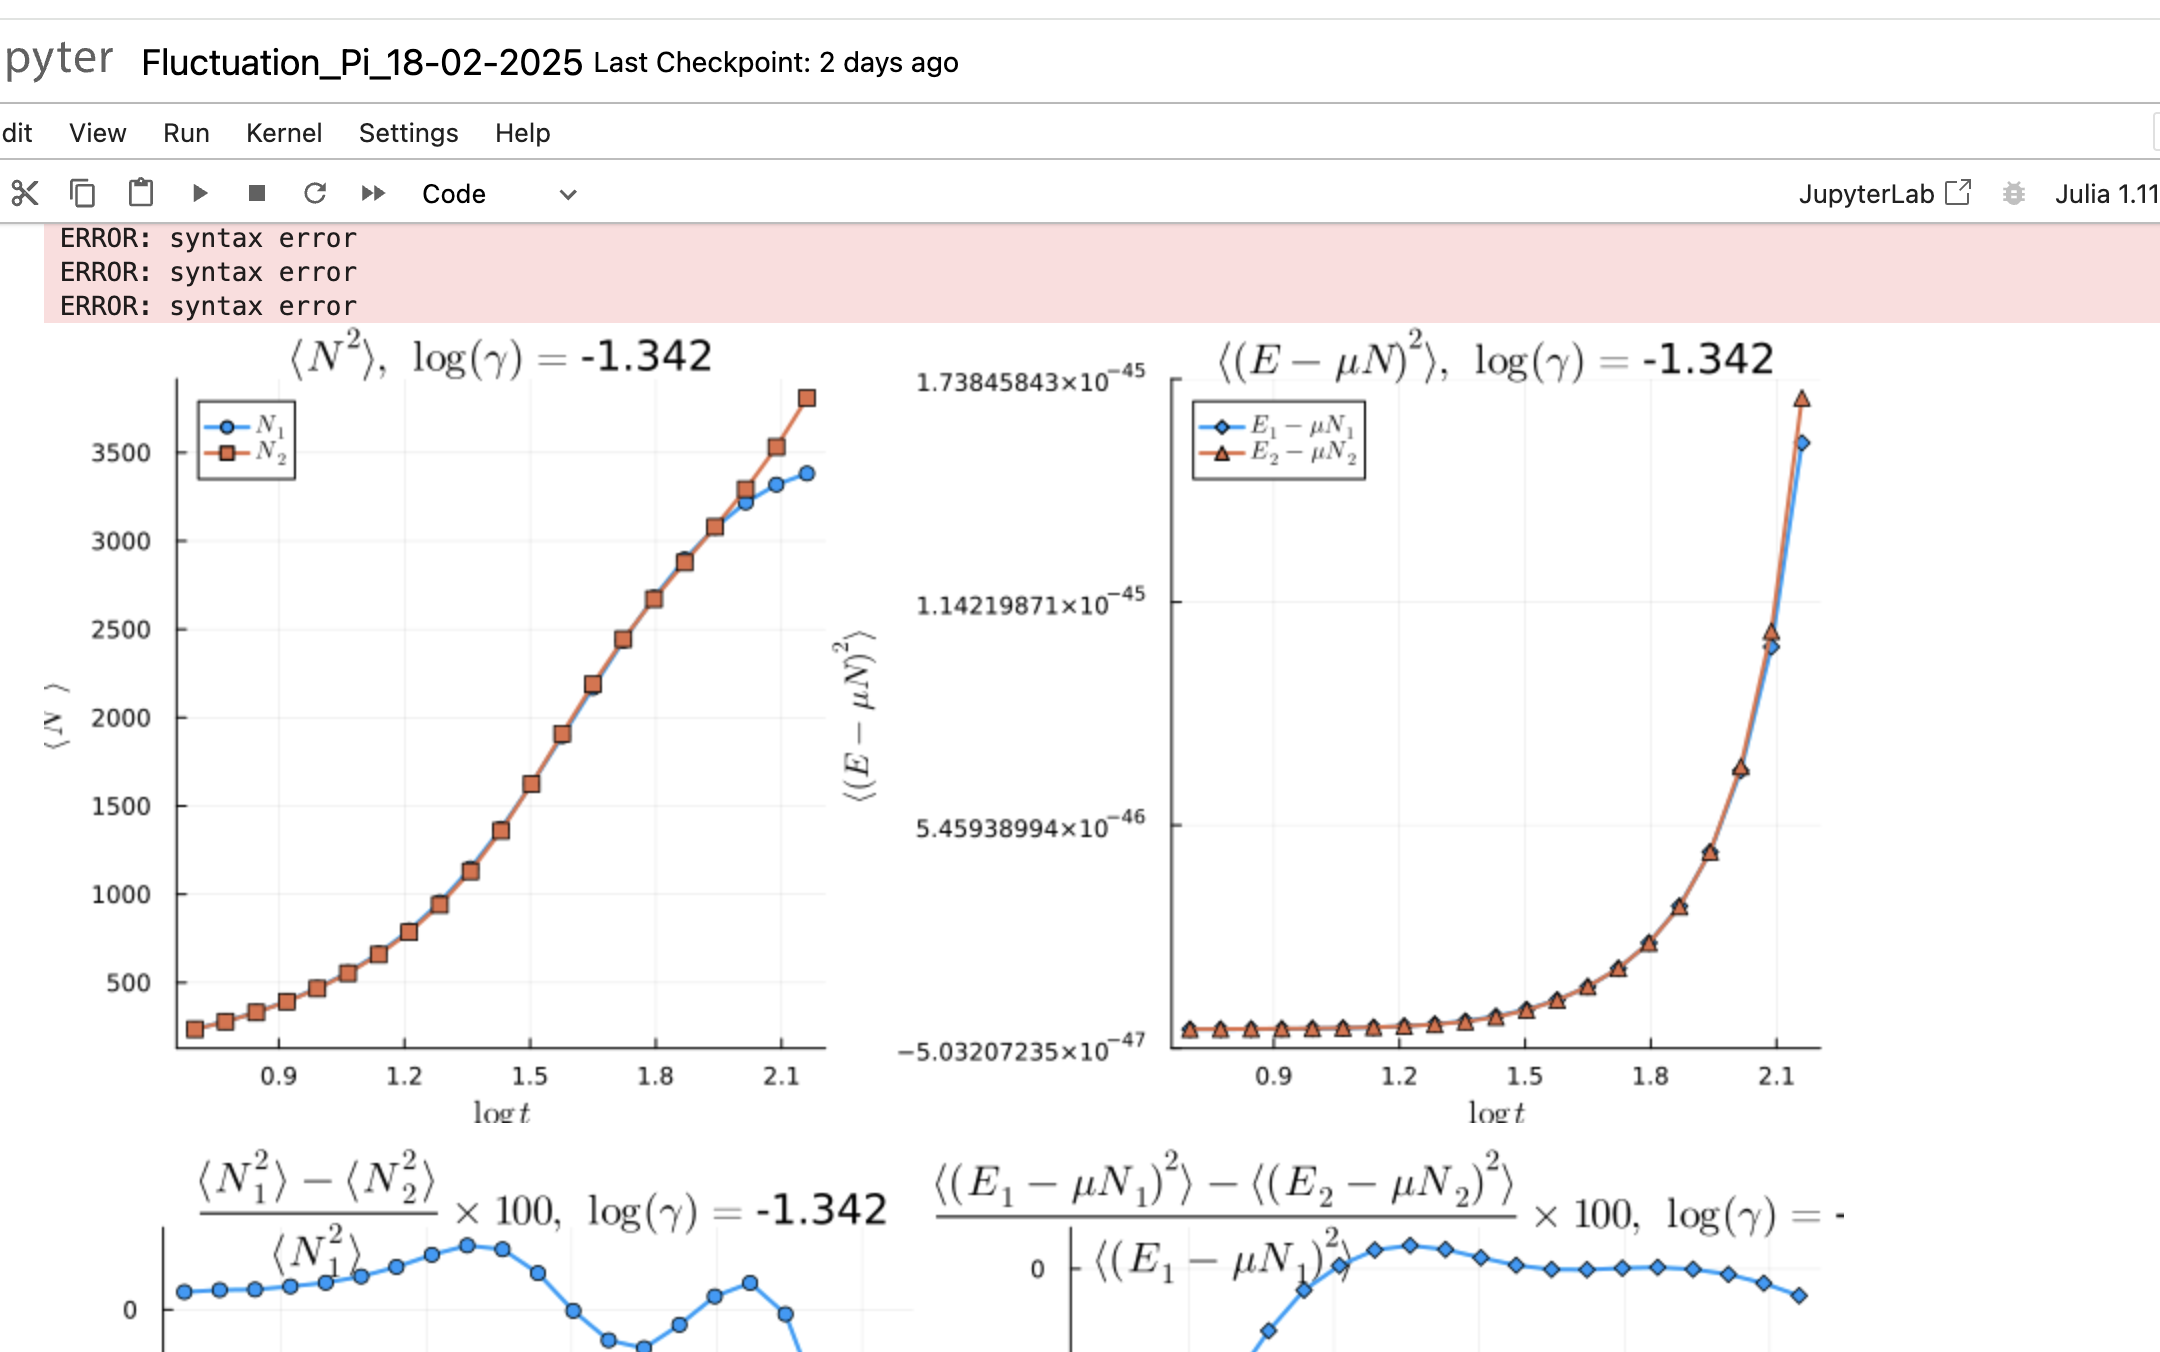
\includegraphics[width=1\textwidth]{Figures/test}

%\begin{aff}
%Donc une a l'ordre un en $\delta \theta (\operator{A}^{(0)})^{-1} %\operator{V}$ 

%\begin{eqnarray*}
%	\langle \delta \Pi ( \theta) \delta \Pi ( \theta') \rangle & = &  ( (\Pi^c_s - \Pi^c)\Pi^c/\Pi^c_s ) ( \theta ) \delta_{\theta, \theta'}/\delta \theta + \mathscr{F}(\theta , \theta' ) ,	
%\end{eqnarray*}

%avec 

%\begin{eqnarray*}
%	\mathscr{F}(\theta , \theta' ) & = & \left [ (\Pi^c_s - \Pi^c )( \theta)  +  (\Pi^c_s - \Pi^c ) ( \theta' )\right ] \frac{\Pi^c}{\Pi^c_s}(\theta)\frac{\Pi^c}{\Pi^c_s}(\theta') \frac{ \Delta( \theta'- \theta )}{ 2 \pi }\\
%	&&  - \left [ (\Pi^c_s - \Pi^c )( \theta)   (\Pi^c_s - \Pi^c ) ( \theta' )\right ] \frac{\Pi^c}{\Pi^c_s}(\theta)\frac{\Pi^c}{\Pi^c_s}(\theta')\int d\theta'' \left (   \frac{ \Pi^c/\Pi^c_s}{\Pi^c_s - \Pi^c} \right )(\theta'') \frac{\Delta(\theta''- \theta)}{2 \pi}\frac{\Delta(\theta''- \theta')}{2 \pi}  	
%\end{eqnarray*}
%\end{aff}



 









\subsection{Vérification explicite de la condition aux limites}
%Dans ce chapitre, nous nous intéressons aux fluctuations de la distribution de rapidité \( \delta \rho \) autour d'une distribution de référence \( \rho^c \), qui maximise la contribution à la fonction de partition des états, exprimée comme une fonctionnelle de la distribution \( \rho \) : 

La fonction de partition des états, s'exprime comme une fonctionnelle de la distribution \( \rho \) : 

\begin{eqnarray*}
	\Xi & = & \sum_\rho \exp \left( -\mathcal{A}(\rho) \right).
\end{eqnarray*}  

Dans la section {\em \bf Entropie de Yang-Yang} (\ref{??}), l'action \( \mathcal{A}(\rho) \) s'écrit sous la forme :  

\begin{eqnarray*}
	\mathcal{A}(\rho) & \doteq & - L\mathcal{S}_{YY}(\rho) + L\int f(\theta) \rho (\theta) \, d\theta,		
\end{eqnarray*}  

où \( \mathcal{S}_{YY} \) est la fonctionnelle d'entropie de Yang-Yang, définie dans (\ref{??}), et \( f \) est la fonction paramétrant les charges, introduite dans (\ref{??}).  

Dans cette même section {\em \bf Entropie de Yang-Yang} (\ref{??}), nous avons établi un lien entre \( f \) et distribution de référence \( \rho^c \), qui maximise la contribution à la fonction de partition des états .\\

On veux tester si nos experience est décrit pas un GGE. Pour cela nous nous intéressons aux fluctuations de la distribution de rapidité \( \delta \rho \) autour \( \rho^c \).

%Nous poursuivons à présent avec cette définition de l'action de classe $\mathcal{C}^2$ et admetant une distribution critique $\rho^c$ tel que sa différentielle en ce point critique soit nulle $d\mathcal{A}_{\rho^c} = 0 $ (\ref{??}) de sorte que d'aprés la formule de Taylor-Youg %afin de déterminer les fluctuations autour de \( \Pi^c \). Pour cela, nous réécrivons l'action sous la forme :  

Nous poursuivons à présent avec cette définition de l'action de classe $\mathcal{C}^2$ et admetant une distribution critique $\rho^c$ tel que sa différentielle en ce point critique soit nulle $d\mathcal{A}_{\rho^c} = 0 $ (\ref{??}) de sorte que d'aprés la formule de Taylor-Youg %afin de déterminer les fluctuations autour de \( \Pi^c \). Pour cela, nous réécrivons l'action sous la forme :  

\begin{eqnarray*}  
	\mathcal{A}(\rho^c + \delta \rho) & \underset{ \delta \rho \to 0 }{=} & \mathcal{A}(\rho^c)  + \frac{1}{2} \left. \frac{\delta^2 \mathcal{A}}{\delta \rho^2} \right|_{\rho^c} (\delta \rho) + \mathcal{O}((\delta \rho)^3),  
\end{eqnarray*}  

une expression quadratique pour l'action à l'ordre dominant en \( \delta \Pi \) avec $\left. \frac{\delta^2 \mathcal{A}}{\delta \rho^2} \right|_{\rho^c}$ la forme quadratique définie positive (Fig (\ref{fig.fluctu.A})).

\begin{figure}[H]
	\centering 
	\begin{tikzpicture}
		\begin{scope}[shift={(0,0)}]
			\begin{scope}[transform canvas={scale=0.6}]
				% Définition des couleurs avec les codes HTML
\definecolor{colorOne}{HTML}{443E46}
\definecolor{colorTwo}{HTML}{F6DEB8}
\definecolor{colorThree}{HTML}{908CA4}
\definecolor{colorFour}{HTML}{57659E}
\definecolor{colorFive}{HTML}{C57284}
\definecolor{colorSix}{HTML}{FF5B69}

% Raccourcis pour les couleurs
\def\colorOne{colorOne}
\def\colorTwo{colorTwo}
\def\colorThree{colorThree}
\def\colorFour{colorFour}
\def\colorFive{colorFive}
\def\colorSix{colorSix}

\def\colorslide{blue!50!black}



\begin{scope}
	% Tracer une courbe lisse entre des points
	\draw[shift={(0,0)} ,\colorOne]
		(-1 , 0 ) edge [thick,line width=0.8ex , ->,>=triangle 45  , \colorOne] node [pos = 1 , below ]{\huge$\rho$}( 5  , 0 )
	;
	\draw[shift={(0,0)}, color=\colorOne]
		(0, -1.0 ) edge [thick,line width=0.8ex , ->,>=triangle 45  ]node [pos=0.9,left=0.2cm ]{\huge$\mathcal{A}(\rho)$}( 0  , 5 )
	;
	\draw[]
		(2.5, 0.12 ) edge [thick,line width=0.8ex ,\colorThree ]node [pos=1,below  ]{\huge$\rho^c$} (2.5, -0.12 )	
	;
	
	\draw[]
		(2.5, -0.12 ) edge [thick,line width=0.4ex , dashed, \colorThree ] (2.5, 5.5 )
		(1.5, 1 ) edge [thick,line width=0.4ex , <->,>=triangle 45  , \colorThree ] (3.5, 1 )
		(-0.3,1) edge [thick,line width=0.4ex  , \colorThree ] node [pos=0,left ]{\huge$\mathcal{A}(\rho^c)$} (0.3, 1 )	
	;
    \draw[thick, line width=0.8ex , \colorFour] plot[smooth, tension=0.7] coordinates {
        (1, 5) (1.6 , 3 ) (2.5, 1) (3.5 , 3 )  (4, 5)
    };		
	
\end{scope}

	
			
			\end{scope}
			
			\draw[color = red , scale = 0.5 , draw = none  ] (-2 , -1) rectangle (5, 6) ; 	
		\end{scope}
		
		\begin{scope}[shift={(19,-1)}]
			\begin{scope}[transform canvas={scale=0.6}]
				% Définition des couleurs avec les codes HTML
\definecolor{colorOne}{HTML}{443E46}
\definecolor{colorTwo}{HTML}{F6DEB8}
\definecolor{colorThree}{HTML}{908CA4}
\definecolor{colorFour}{HTML}{57659E}
\definecolor{colorFive}{HTML}{C57284}
\definecolor{colorSix}{HTML}{FF5B69}

% Raccourcis pour les couleurs
\def\colorOne{colorOne}
\def\colorTwo{colorTwo}
\def\colorThree{colorThree}
\def\colorFour{colorFour}
\def\colorFive{colorFive}
\def\colorSix{colorSix}

\def\colorslide{blue!50!black}

\def\Occupation{
	\def\traitx{0.3}
	\def\traity{0.5}
	\draw[shift={(0,0)}]
		(-13.5 , 0 ) edge [thick,line width=0.8ex ]( -3.2  , 0 )
		( -3.2 - \traitx  , 0 - \traity ) edge [thick,line width=0.8ex ]( -3.2 + \traitx  , 0 + \traity  )
		( -2.8 - \traitx  , 0 - \traity ) edge [thick,line width=0.8ex ]( -2.8 + \traitx  , 0 + \traity  )
		(-2.8 , 0 ) edge [thick,line width=0.8ex ](2.8  , 0 )
		( 2.8 - \traitx  , 0 - \traity ) edge [thick,line width=0.8ex ]( 2.8 + \traitx  , 0 + \traity  )
		( 3.2 - \traitx  , 0 - \traity ) edge [thick,line width=0.8ex ]( 3.2 + \traitx  , 0 + \traity  )
		(3.2, 0 ) edge [thick,line width=0.8ex,->,>=triangle 45 , color = black ]node [pos=1.01,below  ]{\huge$\theta$}	( 13  , 0 )
	;
	\draw[shift={(0,0)}, color=\colorOne]
		(-10.5 , -1.5 ) edge [thick,line width=0.8ex , ->,>=triangle 45  ]( -10.5  , 4.5 )
	;
		
	\foreach \r in {1 , ... , 3 } {
%		\draw[
%		decoration={
%		markings,
%    	mark connection node=my node,
%    	mark=at position 0 with{\node [blue,transform shape] (my node) {\large \r};}},
%		color=gray, thick, 
%		line width=0.5ex] decorate { 
%            (-11.0, \r) -- (-10.1, \r )}
%        ;
        \draw[
			color=\colorOne,
			] 
            (-11.0, \r) edge[color=\colorThree , thick,line width=0.5ex] node [pos=-0.5 ]{\large\color{\colorFour} $\frac{\r}{\delta \theta}$ } (-10.3, \r )
        	;
	
	}
	

	
	% Graduation abcsisse 
	% Définitions des listes
% Definitions of the lists
\def\listetuple{-9/\theta_{1}, -8/\theta_{2} , -5/\theta_{3} , -2/\theta_{a-1} , 0/\theta_{a} , 1/\theta_{a+1} , 2/\theta_{a+2} ,  5/\theta_{N-4} , 7/\theta_{N-3},8/\theta_{N-1},9/\theta_{N} }
\def\listetrais{-12 , -11, -10, -9 , -8 , -7 ,  -6 , -5, -4.5,-4, -2 , -1, 0 , 0.5, 1, 2, 4 , 5 ,  6 , 7 , 8 ,8.5, 9 ,  10 , 11, 12 }

% Loop over listetrais
\foreach \r in \listetrais {
    % Initialize found variable to zero
    % Initialize found variable to zero
    %\pgfmathsetmacro\found{0}
    \global\def\found{0}
    \xdef\nomtheta{}
    
    % Check if \r is in listetuple
    \foreach \x/\y in \listetuple { 
        \ifdim \r pt=\x pt % If \r matches any \x in listetuple
            \global\def\found{1} ;
            \xdef\nomtheta{\y} % Set \nomtheta to the corresponding \y
            %\pgfmathsetmacro\found{1} % Set found to 1            
            %\global\pgfmathsetmacro\found{1}
        \fi
    }
    
    %\node [circle, draw, red] (A) at (\r, 2) {\found , $\nomtheta$};
    
    % Draw the line and display \nomtheta if found
    \ifnum\found=1
        \draw[color=\colorOne, thick, line width=0.5ex] 
            (\r, -0.3) -- (\r, 0.3) node[red , pos=-0.5] {\large $\nomtheta$};
         \filldraw[line width=0.5ex, color=\colorSix, outer color=\colorSix, inner color=\colorSix] 
            (\r, 0) circle (4pt);
    \else 
        % Draw without \nomtheta and add a blue circle if not found
        \draw[color=\colorOne, thick, line width=0.5ex] 
            (\r, -0.3) -- (\r, 0.3);
        \filldraw[line width=0.5ex, color=\colorSix, outer color=\colorTwo, inner color=\colorTwo] 
            (\r, 0) circle (4pt); 
    \fi
}

\def\listetrais{-9.5/\theta_{i-1}/2/3, -6.5/\theta_{i}/1/4  ,   -1.5/\theta_{j}/2/4 , 1.5/\theta_{j+1}/-1/3 , 3.5/\theta_{\ell-1}/1/3 , 6.5/\theta_{\ell}/3/4 , 9.5/\theta(\theta_{\ell+1})/-1/3 };



\foreach \r/\nomx/\y/\ys in \listetrais {
	\draw[
		decoration={
		markings,
    	mark connection node=my node,
    	mark=at position .5 with{\node [blue,transform shape] (my node) {\large \color{\colorFour} $\nomx$};}},
		color=\colorThree , thick, 
		line width=0.5ex] decorate { 
            (\r, 0.12) -- (\r, -1.2)}
        ;
     
     \ifdim \y pt > -1 pt 
     	\draw[
			decoration={
			markings,
    		mark connection node=my node,
    		mark=at position .5 with{\node [blue,transform shape] (my node) {\large \color{\colorFour} $\Pi(\nomx) $};}},
			color=\colorThree, thick, 
			line width=0.5ex] decorate { 
            (\r, \y) -- (\r +3, \y)}
        ;
        \draw[
			decoration={
			markings,
    		mark connection node=my node,
    		mark=at position .5 with{\node [blue,transform shape] (my node) {\large \color{\colorFive} $\Pi_s(\nomx) $};}},
			color=\colorFive, thick, 
			line width=0.5ex] decorate { 
            (\r, \ys) -- (\r +3, \ys)}
        ;
     \fi 
     \ifdim \r pt= -1.5 pt
     	\draw[
     		decoration={
			markings,
    		mark connection node=my node,
    		mark=at position .5 with{\node [blue,transform shape] (my node) {\large \color{\colorFour}  $\delta \theta $};},
    		%mark=at position 0.1  with {\arrow[blue, line width=0.5ex]{<}},
    		%mark=at position 1  with {\arrow[blue, line width=0.5ex]{>}}
    		},
        	color=\colorThree,
        	thick,
        	line width=0.5ex,
        	%arrows={Computer Modern Rightarrow[line cap=round]-Computer Modern Rightarrow[line cap=round]}
   			](\r, -1.2) edge[arrows={Computer Modern Rightarrow[line cap=round]-}] (\r + 0.4, -1.2)decorate {
    		(\r, -1.2) -- (\r + 3, -1.2)}(\r + 2, -1.2) edge[arrows={-Computer Modern Rightarrow[line cap=round]}] (\r + 3, -1.2)
    		;
    \fi
			
	
}


			
}


\begin{scope}
	%\draw[help lines , width=1.5ex] (-8,-3) grid (8,3);\draw[help lines ,width=0.5ex , opacity = 0.5] (-3,-3) grid[step=0.1] (3,3));
	
	%\draw[help lines] 
	%	(-3,-3) edge[width=1.5ex] grid (3,3)	
	%	(-3,-3) edge[width=0.5ex , opacity = 0.5] grid (3,3)	
	%;
	\begin{scope}[shift={(0,1)},rotate=0,opacity=1,color=black]
		\Occupation	
		
		%\node[anchor=east, font=\bfseries] at (-11, 0) {\color{red}\large (T = 0 )} ;	
	\end{scope}
	
	
	
	
	\begin{scope}[shift={(-10.5,7)},rotate=0,opacity=1,color=black]
	
	\begin{scope}[shift={(-0,0)},rotate=0,opacity=1,color=black]
	
		\draw[shift={(0,0)} ,line width=1ex,rounded corners = 1ex,color=\colorOne , opacity =1 ,fill=\colorOne!00 , pattern={north east lines} , pattern color=\colorOne!00 ]
			(0 , -1 ) rectangle (5,1)
		;
		

		\begin{scope}[shift={(0.5,0.5)}]
			\draw[color=\colorOne, thick, line width=0.5ex] 
            (0, -0.3) -- (0, 0.3) ;
            \filldraw[line width=0.5ex, color=\colorSix, outer color=\colorSix, inner color=\colorSix] 
            (0, 0) circle (4pt);
            
            \node[anchor=west, font=\bfseries] at (0.2, 0) {\color{\colorSix}\large : quasi-particule};
		\end{scope}
		
		\begin{scope}[shift={(0.5,-0.5)}]
			\draw[color=\colorOne, thick, line width=0.5ex] 
            (0, -0.3) -- (0, 0.3) ;
            \filldraw[line width=0.5ex, color=\colorSix, outer color=\colorTwo, inner color=\colorTwo] 
            (0, 0) circle (4pt);
            
            \node[anchor=west, font=\bfseries] at (0.2, 0) {\color{\colorSix}\large : hole};
		\end{scope}

	\end{scope}
	
	\begin{scope}[shift={(6,0)},rotate=0,opacity=1,color=black]	
		
		\draw[shift={(0,0)} ,line width=1ex,rounded corners = 1ex,color=\colorOne , opacity =1 ,fill=\colorOne!00 , pattern={north east lines} , pattern color=\colorOne!00 ]
			(0 , -1 ) rectangle (7.5,1)
		;
		
		\node[anchor=west] at (0.5, 0.5) {\color{\colorFour}\large $\Pi$ };\node[anchor=west, font=\bfseries] at (1, 0.5) {\color{\colorFour}\large : quasi-particule distribution};
		
		\node[anchor=west] at (0.5, -0.5) {\color{\colorFour}\large $\Pi_h$ };\node[anchor=west, font=\bfseries] at (1, -0.5) {\color{\colorFour}\large  : hole distribution};
		
	\end{scope}
	
	\begin{scope}[shift={(14.5,0)},rotate=0,opacity=1,color=black]	
		
		\draw[shift={(0,0)} ,line width=1ex,rounded corners = 1ex,color=\colorOne , opacity =1 ,fill=\colorOne!00 , pattern={north east lines} , pattern color=\colorOne!00 ]
			(0 , -0.5 ) rectangle (7.0,0.5)
		;
		
		\node[anchor=west] at (0.2, 0) {\color{\colorFour}\large ${\color{\colorFive}\Pi_s} = \Pi + \Pi_h $ } node[anchor=west , font=\bfseries] at (3.1 , 0 )  {\color{\colorFour}\large {\color{\colorFive} : density of states}};
		
	\end{scope}
	
	
	\end{scope}


		
	
\end{scope}

	
			
			\end{scope}
			\begin{scope}[scale=1]
				\draw[color = red , scale = 1 , draw = none  ] (-1 , -1) rectangle (5, 5) ; 
			\end{scope}	
		\end{scope}

		
				
			
	\end{tikzpicture}	
	\captionsetup{skip=10pt} % Ajoute de l’espace après la légende
	\label{fig.fluctu.A}
\end{figure}


On discrétise l'axe des rapidités en  petite cellule de rapidité $[\theta, \theta+\delta\theta]$, qui contient $L\rho(\theta) \delta \theta$ rapidités. 
	



Avec ces petites tranches, la forme quadratique s’écrit :

\begin{eqnarray*}
    \left. \frac{\delta^2 \mathcal{A}}{{\delta \rho}^2} \right|_{\rho^c}(\delta \rho ) &=&  \sum_{a,b \mid \text{tranche}}  
    \delta \rho(\theta_a)  \frac{\partial^2 \mathcal{A}}{\partial \delta \rho(\theta_a) \partial \delta \rho(\theta_b) } (\rho^c)  \delta \rho(\theta_b).
\end{eqnarray*}
Les fluctuations s’écrivent donc :

\begin{eqnarray*}
    \langle \delta \rho ( \theta) \delta \rho ( \theta') \rangle &=&  
    \frac{ \int d\delta \rho \, \delta \rho(\theta) \delta \rho ( \theta') 
    \exp \left( - \frac{1}{2} \sum_{a,b \mid \text{tranche}}  
    \delta \rho(\theta_a) \frac{\partial^2 \mathcal{A}}{\partial \delta \rho(\theta_a) \partial \delta \rho(\theta_b) } (\rho^c)  \delta \rho(\theta_b) \right) }
    { \int d\delta \Pi  
    \exp \left( - \frac{1}{2} \sum_{a,b \mid \text{tranche}}  
    \delta \rho(\theta_a) \frac{\partial^2 \mathcal{A}}{\partial \delta \rho(\theta_a) \partial \delta \rho(\theta_b) } (\rho^c)  \delta \rho(\theta_b) \right) } \\
    &=& \left( \mathbf{A}^{-1} \right)_{\theta , \theta'}
\end{eqnarray*}


\begin{aff}

\begin{eqnarray*}
	\langle \delta \rho ( \theta) \delta \rho ( \theta') \rangle &=& 	\left( \mathbf{A}^{-1} \right)_{\theta , \theta'}
\end{eqnarray*}

	
avec la  {\em matrice hessienne} $\mathbf{A}_{\theta , \theta'} \equiv \frac{\partial^2 \mathcal{A}}{\partial \delta \rho(\theta) \partial \delta \rho(\theta') }(\rho^c)$, au point critique/ qui maximise la probabilité  $\rho^c=\rho^c_s \nu^c $, s'écrit

\begin{eqnarray*}
	\operator{A} & = & \operator{A}^{(0)} + \delta \theta \operator{V}
\end{eqnarray*}

avec 

\begin{eqnarray*}
	A^{(0)}_{\theta , \theta'}  & = &  L\delta \theta \left ( \frac{ 1}{\rho^c_s ( 1  - \nu^c ) \nu^c } \right )(\theta)    \delta({\theta - \theta '})	,\\
	V_{\theta , \theta'}  &= & L \delta \theta \left \{ - \left [ \left ( \frac{1}{\rho^c_s( 1 - \nu^c) } \right ) ( \theta)  +  \left ( \frac{1}{\rho^c_s( 1 - \nu^c) } \right ) ( \theta' )\right ] \frac{ \Delta( \theta'- \theta )}{ 2 \pi } + \int d\theta''  \left ( \frac{\nu^c}{\rho^c_s( 1 - \nu^c) } \right )(\theta'') \frac{\Delta(\theta''- \theta)}{2 \pi}\frac{\Delta(\theta''- \theta')}{2 \pi}   \right \} 	
\end{eqnarray*}

\end{aff}

\subsection{Testes}

\begin{eqnarray*}
	\Delta_{\operator{\mathcal{N}}}^2  & = &  \frac{1}{\beta} \left . \frac{\partial \langle \operator{\mathcal{N}} \rangle}{\partial \mu} \right )_T \\
	\Delta_{\operator{\mathcal{E}}-\mu \operator{\mathcal{N}}}^2  & = &  - \left . \frac{\partial \langle \operator{\mathcal{E}}-\mu \operator{\mathcal{N}} \rangle}{\partial \beta} \right )_\mu 
\end{eqnarray*}

et 

\begin{eqnarray*}
	\Delta_{\operator{\mathcal{N}}}^2  &= & L^2 \int d\theta_a \int d \theta_b \, \langle \delta \rho(\theta_a) \delta \rho(\theta_b) \rangle \\
	\Delta_{\operator{\mathcal{E}}-\mu \operator{\mathcal{N}}}^2  & = & L^2 \int d\theta_a \int d \theta_b \, \left ( - \mu + \frac{1}2 m \theta_a^2  \right  )\left ( - \mu + \frac{1}2 m \theta_b^2  \right  )  \langle \delta \rho(\theta_a) \delta \rho(\theta_b) \rangle
\end{eqnarray*}

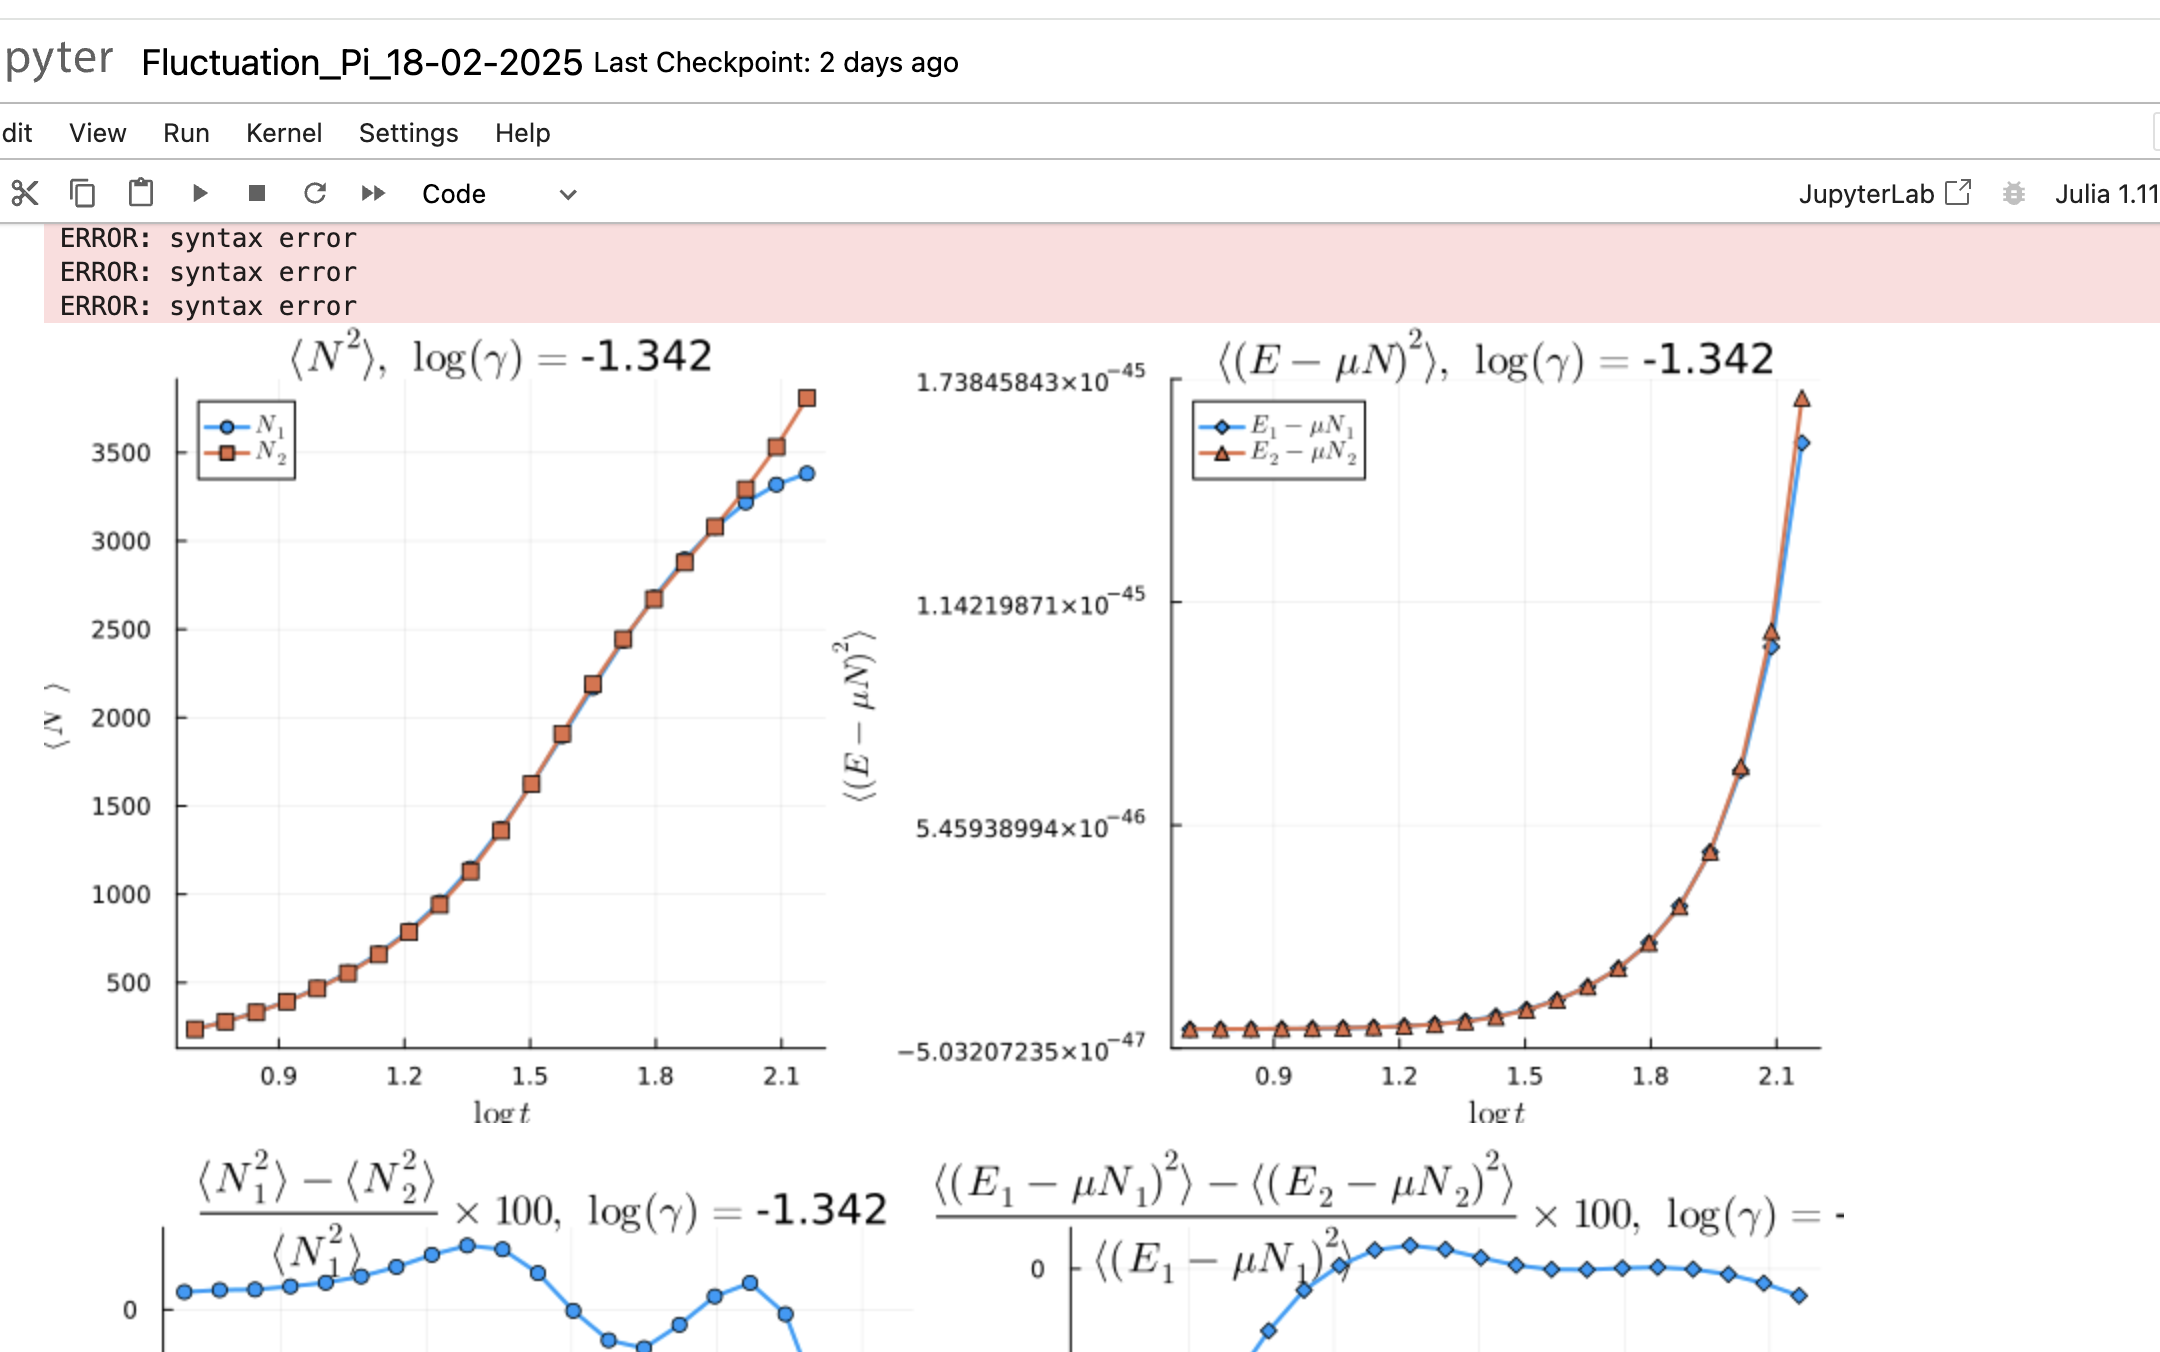
\includegraphics[width=1\textwidth]{Figures/test}

%\begin{aff}
%Donc une a l'ordre un en $\delta \theta (\operator{A}^{(0)})^{-1} %\operator{V}$ 

%\begin{eqnarray*}
%	\langle \delta \Pi ( \theta) \delta \Pi ( \theta') \rangle & = &  ( (\Pi^c_s - \Pi^c)\Pi^c/\Pi^c_s ) ( \theta ) \delta_{\theta, \theta'}/\delta \theta + \mathscr{F}(\theta , \theta' ) ,	
%\end{eqnarray*}

%avec 

%\begin{eqnarray*}
%	\mathscr{F}(\theta , \theta' ) & = & \left [ (\Pi^c_s - \Pi^c )( \theta)  +  (\Pi^c_s - \Pi^c ) ( \theta' )\right ] \frac{\Pi^c}{\Pi^c_s}(\theta)\frac{\Pi^c}{\Pi^c_s}(\theta') \frac{ \Delta( \theta'- \theta )}{ 2 \pi }\\
%	&&  - \left [ (\Pi^c_s - \Pi^c )( \theta)   (\Pi^c_s - \Pi^c ) ( \theta' )\right ] \frac{\Pi^c}{\Pi^c_s}(\theta)\frac{\Pi^c}{\Pi^c_s}(\theta')\int d\theta'' \left (   \frac{ \Pi^c/\Pi^c_s}{\Pi^c_s - \Pi^c} \right )(\theta'') \frac{\Delta(\theta''- \theta)}{2 \pi}\frac{\Delta(\theta''- \theta')}{2 \pi}  	
%\end{eqnarray*}
%\end{aff}



 











\subsection{Lien avec les équations de Bethe}
%Dans ce chapitre, nous nous intéressons aux fluctuations de la distribution de rapidité \( \delta \rho \) autour d'une distribution de référence \( \rho^c \), qui maximise la contribution à la fonction de partition des états, exprimée comme une fonctionnelle de la distribution \( \rho \) : 

La fonction de partition des états, s'exprime comme une fonctionnelle de la distribution \( \rho \) : 

\begin{eqnarray*}
	\Xi & = & \sum_\rho \exp \left( -\mathcal{A}(\rho) \right).
\end{eqnarray*}  

Dans la section {\em \bf Entropie de Yang-Yang} (\ref{??}), l'action \( \mathcal{A}(\rho) \) s'écrit sous la forme :  

\begin{eqnarray*}
	\mathcal{A}(\rho) & \doteq & - L\mathcal{S}_{YY}(\rho) + L\int f(\theta) \rho (\theta) \, d\theta,		
\end{eqnarray*}  

où \( \mathcal{S}_{YY} \) est la fonctionnelle d'entropie de Yang-Yang, définie dans (\ref{??}), et \( f \) est la fonction paramétrant les charges, introduite dans (\ref{??}).  

Dans cette même section {\em \bf Entropie de Yang-Yang} (\ref{??}), nous avons établi un lien entre \( f \) et distribution de référence \( \rho^c \), qui maximise la contribution à la fonction de partition des états .\\

On veux tester si nos experience est décrit pas un GGE. Pour cela nous nous intéressons aux fluctuations de la distribution de rapidité \( \delta \rho \) autour \( \rho^c \).

%Nous poursuivons à présent avec cette définition de l'action de classe $\mathcal{C}^2$ et admetant une distribution critique $\rho^c$ tel que sa différentielle en ce point critique soit nulle $d\mathcal{A}_{\rho^c} = 0 $ (\ref{??}) de sorte que d'aprés la formule de Taylor-Youg %afin de déterminer les fluctuations autour de \( \Pi^c \). Pour cela, nous réécrivons l'action sous la forme :  

Nous poursuivons à présent avec cette définition de l'action de classe $\mathcal{C}^2$ et admetant une distribution critique $\rho^c$ tel que sa différentielle en ce point critique soit nulle $d\mathcal{A}_{\rho^c} = 0 $ (\ref{??}) de sorte que d'aprés la formule de Taylor-Youg %afin de déterminer les fluctuations autour de \( \Pi^c \). Pour cela, nous réécrivons l'action sous la forme :  

\begin{eqnarray*}  
	\mathcal{A}(\rho^c + \delta \rho) & \underset{ \delta \rho \to 0 }{=} & \mathcal{A}(\rho^c)  + \frac{1}{2} \left. \frac{\delta^2 \mathcal{A}}{\delta \rho^2} \right|_{\rho^c} (\delta \rho) + \mathcal{O}((\delta \rho)^3),  
\end{eqnarray*}  

une expression quadratique pour l'action à l'ordre dominant en \( \delta \Pi \) avec $\left. \frac{\delta^2 \mathcal{A}}{\delta \rho^2} \right|_{\rho^c}$ la forme quadratique définie positive (Fig (\ref{fig.fluctu.A})).

\begin{figure}[H]
	\centering 
	\begin{tikzpicture}
		\begin{scope}[shift={(0,0)}]
			\begin{scope}[transform canvas={scale=0.6}]
				% Définition des couleurs avec les codes HTML
\definecolor{colorOne}{HTML}{443E46}
\definecolor{colorTwo}{HTML}{F6DEB8}
\definecolor{colorThree}{HTML}{908CA4}
\definecolor{colorFour}{HTML}{57659E}
\definecolor{colorFive}{HTML}{C57284}
\definecolor{colorSix}{HTML}{FF5B69}

% Raccourcis pour les couleurs
\def\colorOne{colorOne}
\def\colorTwo{colorTwo}
\def\colorThree{colorThree}
\def\colorFour{colorFour}
\def\colorFive{colorFive}
\def\colorSix{colorSix}

\def\colorslide{blue!50!black}



\begin{scope}
	% Tracer une courbe lisse entre des points
	\draw[shift={(0,0)} ,\colorOne]
		(-1 , 0 ) edge [thick,line width=0.8ex , ->,>=triangle 45  , \colorOne] node [pos = 1 , below ]{\huge$\rho$}( 5  , 0 )
	;
	\draw[shift={(0,0)}, color=\colorOne]
		(0, -1.0 ) edge [thick,line width=0.8ex , ->,>=triangle 45  ]node [pos=0.9,left=0.2cm ]{\huge$\mathcal{A}(\rho)$}( 0  , 5 )
	;
	\draw[]
		(2.5, 0.12 ) edge [thick,line width=0.8ex ,\colorThree ]node [pos=1,below  ]{\huge$\rho^c$} (2.5, -0.12 )	
	;
	
	\draw[]
		(2.5, -0.12 ) edge [thick,line width=0.4ex , dashed, \colorThree ] (2.5, 5.5 )
		(1.5, 1 ) edge [thick,line width=0.4ex , <->,>=triangle 45  , \colorThree ] (3.5, 1 )
		(-0.3,1) edge [thick,line width=0.4ex  , \colorThree ] node [pos=0,left ]{\huge$\mathcal{A}(\rho^c)$} (0.3, 1 )	
	;
    \draw[thick, line width=0.8ex , \colorFour] plot[smooth, tension=0.7] coordinates {
        (1, 5) (1.6 , 3 ) (2.5, 1) (3.5 , 3 )  (4, 5)
    };		
	
\end{scope}

	
			
			\end{scope}
			
			\draw[color = red , scale = 0.5 , draw = none  ] (-2 , -1) rectangle (5, 6) ; 	
		\end{scope}
		
		\begin{scope}[shift={(19,-1)}]
			\begin{scope}[transform canvas={scale=0.6}]
				% Définition des couleurs avec les codes HTML
\definecolor{colorOne}{HTML}{443E46}
\definecolor{colorTwo}{HTML}{F6DEB8}
\definecolor{colorThree}{HTML}{908CA4}
\definecolor{colorFour}{HTML}{57659E}
\definecolor{colorFive}{HTML}{C57284}
\definecolor{colorSix}{HTML}{FF5B69}

% Raccourcis pour les couleurs
\def\colorOne{colorOne}
\def\colorTwo{colorTwo}
\def\colorThree{colorThree}
\def\colorFour{colorFour}
\def\colorFive{colorFive}
\def\colorSix{colorSix}

\def\colorslide{blue!50!black}

\def\Occupation{
	\def\traitx{0.3}
	\def\traity{0.5}
	\draw[shift={(0,0)}]
		(-13.5 , 0 ) edge [thick,line width=0.8ex ]( -3.2  , 0 )
		( -3.2 - \traitx  , 0 - \traity ) edge [thick,line width=0.8ex ]( -3.2 + \traitx  , 0 + \traity  )
		( -2.8 - \traitx  , 0 - \traity ) edge [thick,line width=0.8ex ]( -2.8 + \traitx  , 0 + \traity  )
		(-2.8 , 0 ) edge [thick,line width=0.8ex ](2.8  , 0 )
		( 2.8 - \traitx  , 0 - \traity ) edge [thick,line width=0.8ex ]( 2.8 + \traitx  , 0 + \traity  )
		( 3.2 - \traitx  , 0 - \traity ) edge [thick,line width=0.8ex ]( 3.2 + \traitx  , 0 + \traity  )
		(3.2, 0 ) edge [thick,line width=0.8ex,->,>=triangle 45 , color = black ]node [pos=1.01,below  ]{\huge$\theta$}	( 13  , 0 )
	;
	\draw[shift={(0,0)}, color=\colorOne]
		(-10.5 , -1.5 ) edge [thick,line width=0.8ex , ->,>=triangle 45  ]( -10.5  , 4.5 )
	;
		
	\foreach \r in {1 , ... , 3 } {
%		\draw[
%		decoration={
%		markings,
%    	mark connection node=my node,
%    	mark=at position 0 with{\node [blue,transform shape] (my node) {\large \r};}},
%		color=gray, thick, 
%		line width=0.5ex] decorate { 
%            (-11.0, \r) -- (-10.1, \r )}
%        ;
        \draw[
			color=\colorOne,
			] 
            (-11.0, \r) edge[color=\colorThree , thick,line width=0.5ex] node [pos=-0.5 ]{\large\color{\colorFour} $\frac{\r}{\delta \theta}$ } (-10.3, \r )
        	;
	
	}
	

	
	% Graduation abcsisse 
	% Définitions des listes
% Definitions of the lists
\def\listetuple{-9/\theta_{1}, -8/\theta_{2} , -5/\theta_{3} , -2/\theta_{a-1} , 0/\theta_{a} , 1/\theta_{a+1} , 2/\theta_{a+2} ,  5/\theta_{N-4} , 7/\theta_{N-3},8/\theta_{N-1},9/\theta_{N} }
\def\listetrais{-12 , -11, -10, -9 , -8 , -7 ,  -6 , -5, -4.5,-4, -2 , -1, 0 , 0.5, 1, 2, 4 , 5 ,  6 , 7 , 8 ,8.5, 9 ,  10 , 11, 12 }

% Loop over listetrais
\foreach \r in \listetrais {
    % Initialize found variable to zero
    % Initialize found variable to zero
    %\pgfmathsetmacro\found{0}
    \global\def\found{0}
    \xdef\nomtheta{}
    
    % Check if \r is in listetuple
    \foreach \x/\y in \listetuple { 
        \ifdim \r pt=\x pt % If \r matches any \x in listetuple
            \global\def\found{1} ;
            \xdef\nomtheta{\y} % Set \nomtheta to the corresponding \y
            %\pgfmathsetmacro\found{1} % Set found to 1            
            %\global\pgfmathsetmacro\found{1}
        \fi
    }
    
    %\node [circle, draw, red] (A) at (\r, 2) {\found , $\nomtheta$};
    
    % Draw the line and display \nomtheta if found
    \ifnum\found=1
        \draw[color=\colorOne, thick, line width=0.5ex] 
            (\r, -0.3) -- (\r, 0.3) node[red , pos=-0.5] {\large $\nomtheta$};
         \filldraw[line width=0.5ex, color=\colorSix, outer color=\colorSix, inner color=\colorSix] 
            (\r, 0) circle (4pt);
    \else 
        % Draw without \nomtheta and add a blue circle if not found
        \draw[color=\colorOne, thick, line width=0.5ex] 
            (\r, -0.3) -- (\r, 0.3);
        \filldraw[line width=0.5ex, color=\colorSix, outer color=\colorTwo, inner color=\colorTwo] 
            (\r, 0) circle (4pt); 
    \fi
}

\def\listetrais{-9.5/\theta_{i-1}/2/3, -6.5/\theta_{i}/1/4  ,   -1.5/\theta_{j}/2/4 , 1.5/\theta_{j+1}/-1/3 , 3.5/\theta_{\ell-1}/1/3 , 6.5/\theta_{\ell}/3/4 , 9.5/\theta(\theta_{\ell+1})/-1/3 };



\foreach \r/\nomx/\y/\ys in \listetrais {
	\draw[
		decoration={
		markings,
    	mark connection node=my node,
    	mark=at position .5 with{\node [blue,transform shape] (my node) {\large \color{\colorFour} $\nomx$};}},
		color=\colorThree , thick, 
		line width=0.5ex] decorate { 
            (\r, 0.12) -- (\r, -1.2)}
        ;
     
     \ifdim \y pt > -1 pt 
     	\draw[
			decoration={
			markings,
    		mark connection node=my node,
    		mark=at position .5 with{\node [blue,transform shape] (my node) {\large \color{\colorFour} $\Pi(\nomx) $};}},
			color=\colorThree, thick, 
			line width=0.5ex] decorate { 
            (\r, \y) -- (\r +3, \y)}
        ;
        \draw[
			decoration={
			markings,
    		mark connection node=my node,
    		mark=at position .5 with{\node [blue,transform shape] (my node) {\large \color{\colorFive} $\Pi_s(\nomx) $};}},
			color=\colorFive, thick, 
			line width=0.5ex] decorate { 
            (\r, \ys) -- (\r +3, \ys)}
        ;
     \fi 
     \ifdim \r pt= -1.5 pt
     	\draw[
     		decoration={
			markings,
    		mark connection node=my node,
    		mark=at position .5 with{\node [blue,transform shape] (my node) {\large \color{\colorFour}  $\delta \theta $};},
    		%mark=at position 0.1  with {\arrow[blue, line width=0.5ex]{<}},
    		%mark=at position 1  with {\arrow[blue, line width=0.5ex]{>}}
    		},
        	color=\colorThree,
        	thick,
        	line width=0.5ex,
        	%arrows={Computer Modern Rightarrow[line cap=round]-Computer Modern Rightarrow[line cap=round]}
   			](\r, -1.2) edge[arrows={Computer Modern Rightarrow[line cap=round]-}] (\r + 0.4, -1.2)decorate {
    		(\r, -1.2) -- (\r + 3, -1.2)}(\r + 2, -1.2) edge[arrows={-Computer Modern Rightarrow[line cap=round]}] (\r + 3, -1.2)
    		;
    \fi
			
	
}


			
}


\begin{scope}
	%\draw[help lines , width=1.5ex] (-8,-3) grid (8,3);\draw[help lines ,width=0.5ex , opacity = 0.5] (-3,-3) grid[step=0.1] (3,3));
	
	%\draw[help lines] 
	%	(-3,-3) edge[width=1.5ex] grid (3,3)	
	%	(-3,-3) edge[width=0.5ex , opacity = 0.5] grid (3,3)	
	%;
	\begin{scope}[shift={(0,1)},rotate=0,opacity=1,color=black]
		\Occupation	
		
		%\node[anchor=east, font=\bfseries] at (-11, 0) {\color{red}\large (T = 0 )} ;	
	\end{scope}
	
	
	
	
	\begin{scope}[shift={(-10.5,7)},rotate=0,opacity=1,color=black]
	
	\begin{scope}[shift={(-0,0)},rotate=0,opacity=1,color=black]
	
		\draw[shift={(0,0)} ,line width=1ex,rounded corners = 1ex,color=\colorOne , opacity =1 ,fill=\colorOne!00 , pattern={north east lines} , pattern color=\colorOne!00 ]
			(0 , -1 ) rectangle (5,1)
		;
		

		\begin{scope}[shift={(0.5,0.5)}]
			\draw[color=\colorOne, thick, line width=0.5ex] 
            (0, -0.3) -- (0, 0.3) ;
            \filldraw[line width=0.5ex, color=\colorSix, outer color=\colorSix, inner color=\colorSix] 
            (0, 0) circle (4pt);
            
            \node[anchor=west, font=\bfseries] at (0.2, 0) {\color{\colorSix}\large : quasi-particule};
		\end{scope}
		
		\begin{scope}[shift={(0.5,-0.5)}]
			\draw[color=\colorOne, thick, line width=0.5ex] 
            (0, -0.3) -- (0, 0.3) ;
            \filldraw[line width=0.5ex, color=\colorSix, outer color=\colorTwo, inner color=\colorTwo] 
            (0, 0) circle (4pt);
            
            \node[anchor=west, font=\bfseries] at (0.2, 0) {\color{\colorSix}\large : hole};
		\end{scope}

	\end{scope}
	
	\begin{scope}[shift={(6,0)},rotate=0,opacity=1,color=black]	
		
		\draw[shift={(0,0)} ,line width=1ex,rounded corners = 1ex,color=\colorOne , opacity =1 ,fill=\colorOne!00 , pattern={north east lines} , pattern color=\colorOne!00 ]
			(0 , -1 ) rectangle (7.5,1)
		;
		
		\node[anchor=west] at (0.5, 0.5) {\color{\colorFour}\large $\Pi$ };\node[anchor=west, font=\bfseries] at (1, 0.5) {\color{\colorFour}\large : quasi-particule distribution};
		
		\node[anchor=west] at (0.5, -0.5) {\color{\colorFour}\large $\Pi_h$ };\node[anchor=west, font=\bfseries] at (1, -0.5) {\color{\colorFour}\large  : hole distribution};
		
	\end{scope}
	
	\begin{scope}[shift={(14.5,0)},rotate=0,opacity=1,color=black]	
		
		\draw[shift={(0,0)} ,line width=1ex,rounded corners = 1ex,color=\colorOne , opacity =1 ,fill=\colorOne!00 , pattern={north east lines} , pattern color=\colorOne!00 ]
			(0 , -0.5 ) rectangle (7.0,0.5)
		;
		
		\node[anchor=west] at (0.2, 0) {\color{\colorFour}\large ${\color{\colorFive}\Pi_s} = \Pi + \Pi_h $ } node[anchor=west , font=\bfseries] at (3.1 , 0 )  {\color{\colorFour}\large {\color{\colorFive} : density of states}};
		
	\end{scope}
	
	
	\end{scope}


		
	
\end{scope}

	
			
			\end{scope}
			\begin{scope}[scale=1]
				\draw[color = red , scale = 1 , draw = none  ] (-1 , -1) rectangle (5, 5) ; 
			\end{scope}	
		\end{scope}

		
				
			
	\end{tikzpicture}	
	\captionsetup{skip=10pt} % Ajoute de l’espace après la légende
	\label{fig.fluctu.A}
\end{figure}


On discrétise l'axe des rapidités en  petite cellule de rapidité $[\theta, \theta+\delta\theta]$, qui contient $L\rho(\theta) \delta \theta$ rapidités. 
	



Avec ces petites tranches, la forme quadratique s’écrit :

\begin{eqnarray*}
    \left. \frac{\delta^2 \mathcal{A}}{{\delta \rho}^2} \right|_{\rho^c}(\delta \rho ) &=&  \sum_{a,b \mid \text{tranche}}  
    \delta \rho(\theta_a)  \frac{\partial^2 \mathcal{A}}{\partial \delta \rho(\theta_a) \partial \delta \rho(\theta_b) } (\rho^c)  \delta \rho(\theta_b).
\end{eqnarray*}
Les fluctuations s’écrivent donc :

\begin{eqnarray*}
    \langle \delta \rho ( \theta) \delta \rho ( \theta') \rangle &=&  
    \frac{ \int d\delta \rho \, \delta \rho(\theta) \delta \rho ( \theta') 
    \exp \left( - \frac{1}{2} \sum_{a,b \mid \text{tranche}}  
    \delta \rho(\theta_a) \frac{\partial^2 \mathcal{A}}{\partial \delta \rho(\theta_a) \partial \delta \rho(\theta_b) } (\rho^c)  \delta \rho(\theta_b) \right) }
    { \int d\delta \Pi  
    \exp \left( - \frac{1}{2} \sum_{a,b \mid \text{tranche}}  
    \delta \rho(\theta_a) \frac{\partial^2 \mathcal{A}}{\partial \delta \rho(\theta_a) \partial \delta \rho(\theta_b) } (\rho^c)  \delta \rho(\theta_b) \right) } \\
    &=& \left( \mathbf{A}^{-1} \right)_{\theta , \theta'}
\end{eqnarray*}


\begin{aff}

\begin{eqnarray*}
	\langle \delta \rho ( \theta) \delta \rho ( \theta') \rangle &=& 	\left( \mathbf{A}^{-1} \right)_{\theta , \theta'}
\end{eqnarray*}

	
avec la  {\em matrice hessienne} $\mathbf{A}_{\theta , \theta'} \equiv \frac{\partial^2 \mathcal{A}}{\partial \delta \rho(\theta) \partial \delta \rho(\theta') }(\rho^c)$, au point critique/ qui maximise la probabilité  $\rho^c=\rho^c_s \nu^c $, s'écrit

\begin{eqnarray*}
	\operator{A} & = & \operator{A}^{(0)} + \delta \theta \operator{V}
\end{eqnarray*}

avec 

\begin{eqnarray*}
	A^{(0)}_{\theta , \theta'}  & = &  L\delta \theta \left ( \frac{ 1}{\rho^c_s ( 1  - \nu^c ) \nu^c } \right )(\theta)    \delta({\theta - \theta '})	,\\
	V_{\theta , \theta'}  &= & L \delta \theta \left \{ - \left [ \left ( \frac{1}{\rho^c_s( 1 - \nu^c) } \right ) ( \theta)  +  \left ( \frac{1}{\rho^c_s( 1 - \nu^c) } \right ) ( \theta' )\right ] \frac{ \Delta( \theta'- \theta )}{ 2 \pi } + \int d\theta''  \left ( \frac{\nu^c}{\rho^c_s( 1 - \nu^c) } \right )(\theta'') \frac{\Delta(\theta''- \theta)}{2 \pi}\frac{\Delta(\theta''- \theta')}{2 \pi}   \right \} 	
\end{eqnarray*}

\end{aff}

\subsection{Testes}

\begin{eqnarray*}
	\Delta_{\operator{\mathcal{N}}}^2  & = &  \frac{1}{\beta} \left . \frac{\partial \langle \operator{\mathcal{N}} \rangle}{\partial \mu} \right )_T \\
	\Delta_{\operator{\mathcal{E}}-\mu \operator{\mathcal{N}}}^2  & = &  - \left . \frac{\partial \langle \operator{\mathcal{E}}-\mu \operator{\mathcal{N}} \rangle}{\partial \beta} \right )_\mu 
\end{eqnarray*}

et 

\begin{eqnarray*}
	\Delta_{\operator{\mathcal{N}}}^2  &= & L^2 \int d\theta_a \int d \theta_b \, \langle \delta \rho(\theta_a) \delta \rho(\theta_b) \rangle \\
	\Delta_{\operator{\mathcal{E}}-\mu \operator{\mathcal{N}}}^2  & = & L^2 \int d\theta_a \int d \theta_b \, \left ( - \mu + \frac{1}2 m \theta_a^2  \right  )\left ( - \mu + \frac{1}2 m \theta_b^2  \right  )  \langle \delta \rho(\theta_a) \delta \rho(\theta_b) \rangle
\end{eqnarray*}

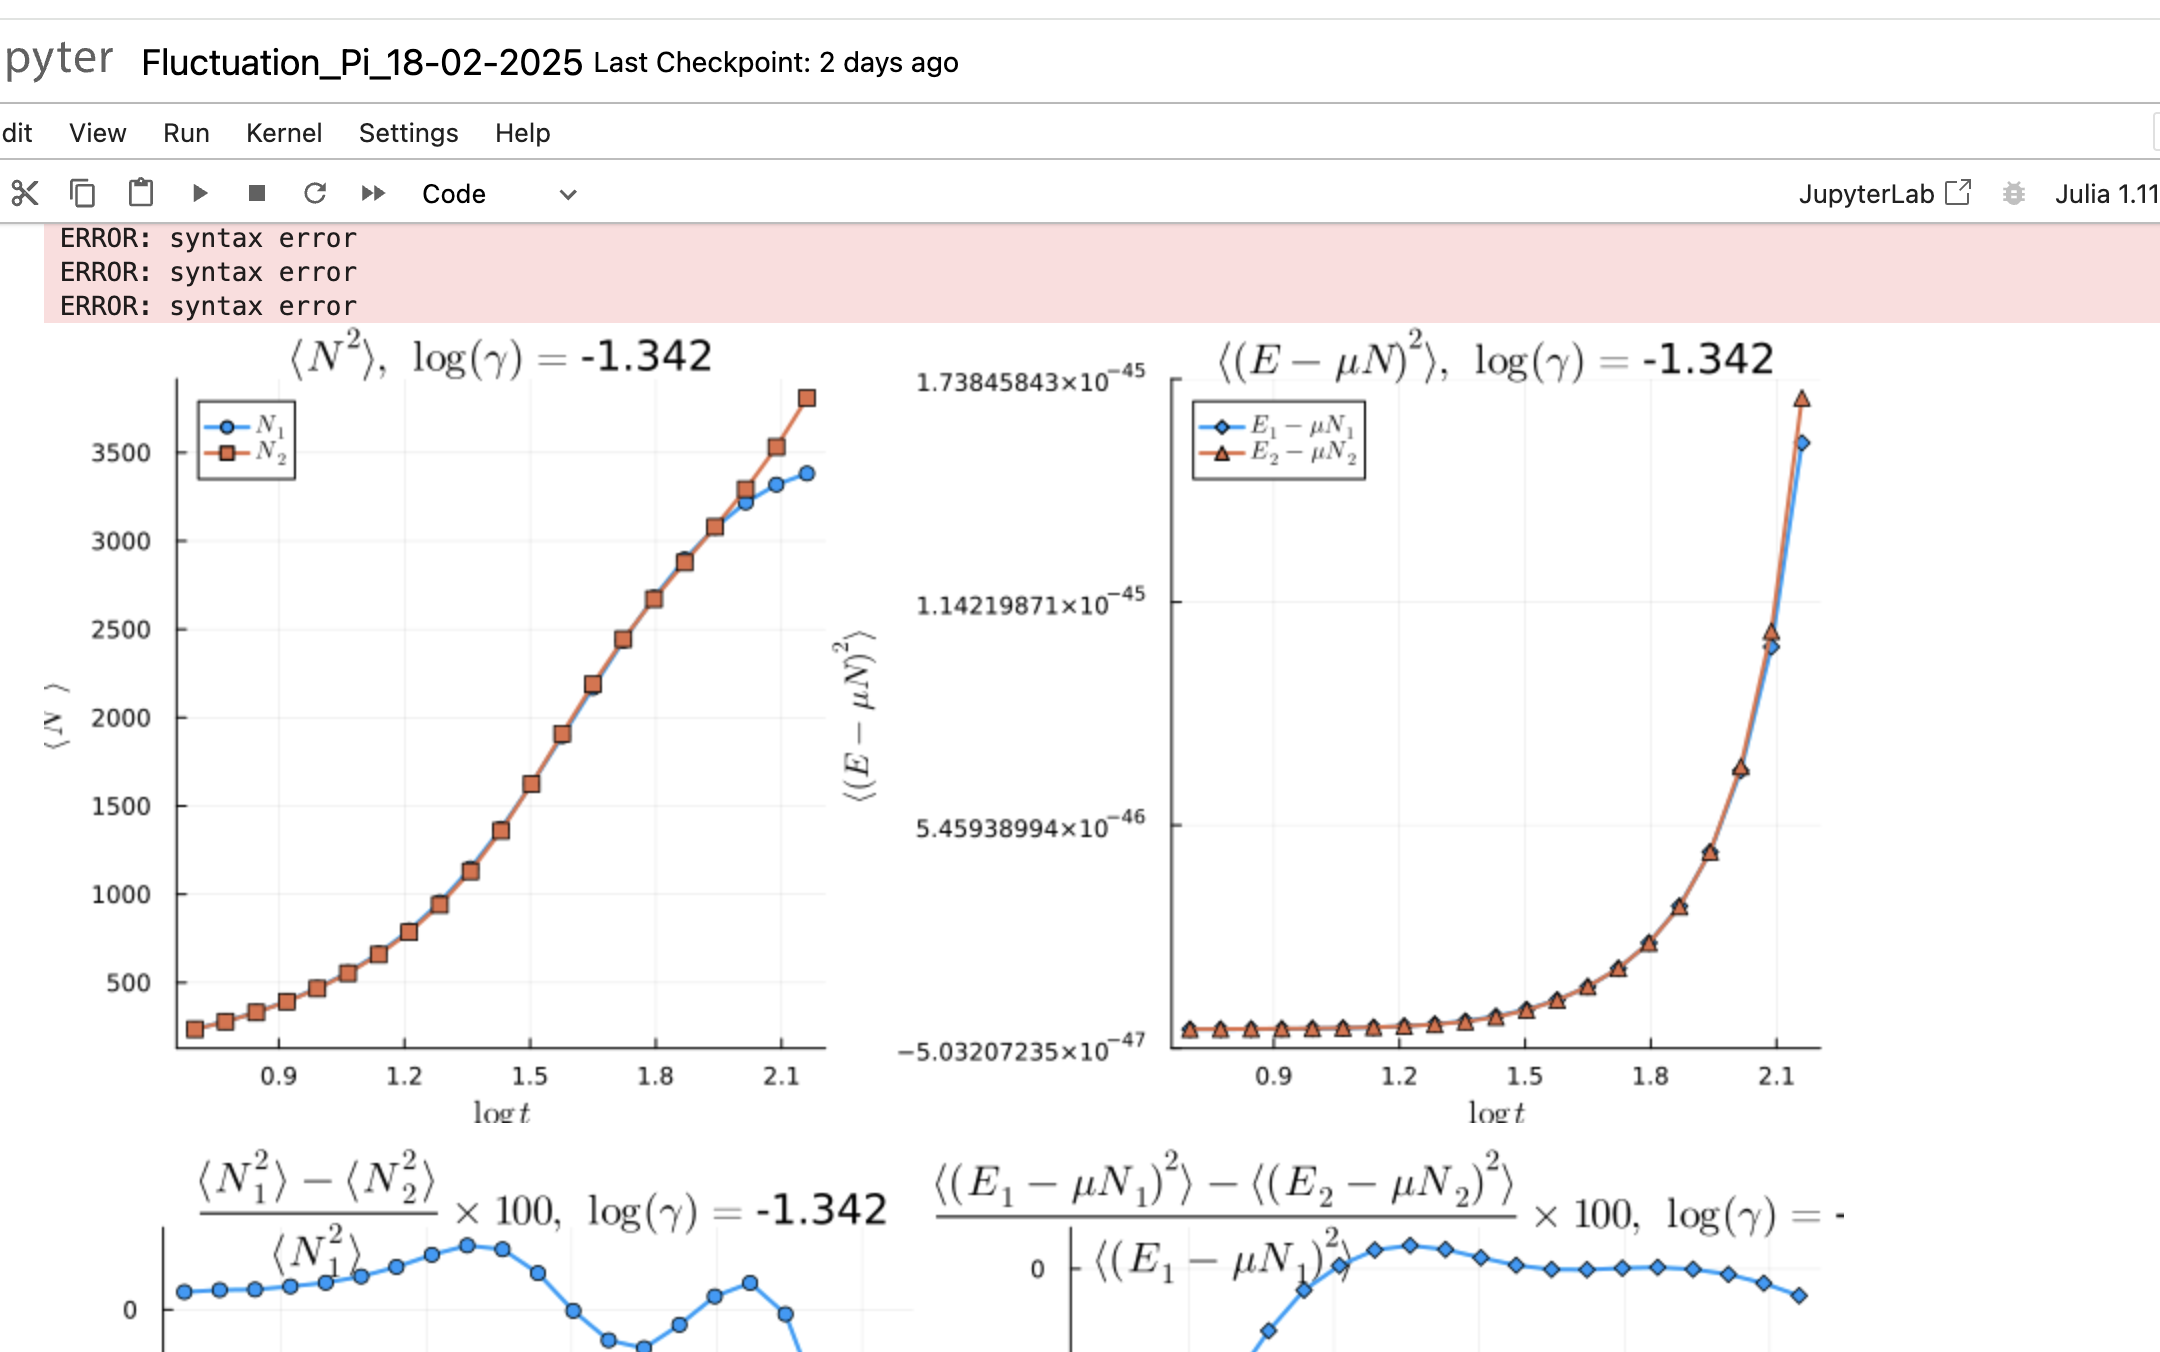
\includegraphics[width=1\textwidth]{Figures/test}

%\begin{aff}
%Donc une a l'ordre un en $\delta \theta (\operator{A}^{(0)})^{-1} %\operator{V}$ 

%\begin{eqnarray*}
%	\langle \delta \Pi ( \theta) \delta \Pi ( \theta') \rangle & = &  ( (\Pi^c_s - \Pi^c)\Pi^c/\Pi^c_s ) ( \theta ) \delta_{\theta, \theta'}/\delta \theta + \mathscr{F}(\theta , \theta' ) ,	
%\end{eqnarray*}

%avec 

%\begin{eqnarray*}
%	\mathscr{F}(\theta , \theta' ) & = & \left [ (\Pi^c_s - \Pi^c )( \theta)  +  (\Pi^c_s - \Pi^c ) ( \theta' )\right ] \frac{\Pi^c}{\Pi^c_s}(\theta)\frac{\Pi^c}{\Pi^c_s}(\theta') \frac{ \Delta( \theta'- \theta )}{ 2 \pi }\\
%	&&  - \left [ (\Pi^c_s - \Pi^c )( \theta)   (\Pi^c_s - \Pi^c ) ( \theta' )\right ] \frac{\Pi^c}{\Pi^c_s}(\theta)\frac{\Pi^c}{\Pi^c_s}(\theta')\int d\theta'' \left (   \frac{ \Pi^c/\Pi^c_s}{\Pi^c_s - \Pi^c} \right )(\theta'') \frac{\Delta(\theta''- \theta)}{2 \pi}\frac{\Delta(\theta''- \theta')}{2 \pi}  	
%\end{eqnarray*}
%\end{aff}



 












\subsection{Introduction au modèle de gaz de Bose unidimensionnel et Hamiltonien du modèle}
%\paragraph{Why Second Quantification ?}

\subparagraph{First Quantification (Single Particle)}
\begin{itemize}[label = $\bullet$]
	\item In first quantification, promote classical observable $x$, $p$ of a single particle to operators  $\operator{x}$ , $\operator{p}$  acting on wavefunctions $\psi(x)$.
\end{itemize}


\subparagraph{The Many-Body Problem}
\begin{itemize}[label = $\bullet$]
	\item When we try to describe $N$ identical particles, we write a wavefunction $\Psi(x_1 , x_2 , \cdots , x_N )$ of $N$ variables.
	\item Enforcing the fact that "particles are identical" means $Psi$ must be symmetric (for bosons) or antisymmetric (for fermions) under swapping any pair of $x_i \leftrightarrow x_j$.
	\item As $N$ grows, these symmetrized wavefunctions becomes hard to deal with.
\end{itemize}

\subparagraph{Second Quantification}
\begin{itemize}[label = $\bullet$]
	\item Instead of labeling each particle by coordinates $(x_1 , x_2 , \cdots )$, we switch to describing "how many particles live in each possible single-particle state."
	\item Think of having a list of available one-particle "modes" (e.g. energy levels. plane-wave states, etc.) We then say: "There are $n_1$ particles in mode $1$ , $n_2$ particles in mode $2$, and so on." 
	\item This viewpoint automatically takes care of (anti)symmetry for us. We only keep track of {bf occupation numbers} $n_i$, not which specific particle is where.	
\end{itemize}

\paragraph{Pourquoi la seconde quantification ?}
\subparagraph{Première quantification (particule unique)}
\begin{itemize}[label = $\bullet$]
\item Dans la première quantification, on promeut les observables classiques $x$ et $p$ d’une particule unique en opérateurs $\hat{x}$ et $\hat{p}$ agissant sur les fonctions d’onde $\psi(x)$.
\end{itemize}

\subparagraph{Le problème à plusieurs corps}
\begin{itemize}[label = $\bullet$]
\item Lorsqu’on cherche à décrire un système de $N$ particules identiques, on introduit une fonction d’onde $\Psi(x_1, x_2, \cdots, x_N)$ dépendant de $N$ variables.
\item Le fait que les particules soient indiscernables impose que $\Psi$ soit symétrique (pour des bosons) ou antisymétrique (pour des fermions) sous l’échange de deux coordonnées $x_i \leftrightarrow x_j$.
\item Lorsque $N$ devient grand, manipuler explicitement ces fonctions d’onde (anti)symétrisées devient rapidement incommode et complexe.
\end{itemize}

\subparagraph{Seconde quantification}
\begin{itemize}[label = $\bullet$]
\item Au lieu d’indexer chaque particule par ses coordonnées $(x_1, x_2, \cdots)$, on adopte un formalisme où l’on décrit combien de particules occupent chaque état à une particule.
\item On considère une base d’états à une particule (par exemple : niveaux d’énergie, états d’onde plane, etc.) et on énumère : "il y a $n_1$ particules dans le mode $1$, $n_2$ dans le mode $2$, etc."
\item Cette approche gère automatiquement les contraintes de symétrie : on ne suit plus chaque particule individuellement, mais uniquement les nombres d’occupation $n_i$.
\end{itemize}


%Dans ce chapitre, nous nous intéressons aux fluctuations de la distribution de rapidité \( \delta \rho \) autour d'une distribution de référence \( \rho^c \), qui maximise la contribution à la fonction de partition des états, exprimée comme une fonctionnelle de la distribution \( \rho \) : 

La fonction de partition des états, s'exprime comme une fonctionnelle de la distribution \( \rho \) : 

\begin{eqnarray*}
	\Xi & = & \sum_\rho \exp \left( -\mathcal{A}(\rho) \right).
\end{eqnarray*}  

Dans la section {\em \bf Entropie de Yang-Yang} (\ref{??}), l'action \( \mathcal{A}(\rho) \) s'écrit sous la forme :  

\begin{eqnarray*}
	\mathcal{A}(\rho) & \doteq & - L\mathcal{S}_{YY}(\rho) + L\int f(\theta) \rho (\theta) \, d\theta,		
\end{eqnarray*}  

où \( \mathcal{S}_{YY} \) est la fonctionnelle d'entropie de Yang-Yang, définie dans (\ref{??}), et \( f \) est la fonction paramétrant les charges, introduite dans (\ref{??}).  

Dans cette même section {\em \bf Entropie de Yang-Yang} (\ref{??}), nous avons établi un lien entre \( f \) et distribution de référence \( \rho^c \), qui maximise la contribution à la fonction de partition des états .\\

On veux tester si nos experience est décrit pas un GGE. Pour cela nous nous intéressons aux fluctuations de la distribution de rapidité \( \delta \rho \) autour \( \rho^c \).

%Nous poursuivons à présent avec cette définition de l'action de classe $\mathcal{C}^2$ et admetant une distribution critique $\rho^c$ tel que sa différentielle en ce point critique soit nulle $d\mathcal{A}_{\rho^c} = 0 $ (\ref{??}) de sorte que d'aprés la formule de Taylor-Youg %afin de déterminer les fluctuations autour de \( \Pi^c \). Pour cela, nous réécrivons l'action sous la forme :  

Nous poursuivons à présent avec cette définition de l'action de classe $\mathcal{C}^2$ et admetant une distribution critique $\rho^c$ tel que sa différentielle en ce point critique soit nulle $d\mathcal{A}_{\rho^c} = 0 $ (\ref{??}) de sorte que d'aprés la formule de Taylor-Youg %afin de déterminer les fluctuations autour de \( \Pi^c \). Pour cela, nous réécrivons l'action sous la forme :  

\begin{eqnarray*}  
	\mathcal{A}(\rho^c + \delta \rho) & \underset{ \delta \rho \to 0 }{=} & \mathcal{A}(\rho^c)  + \frac{1}{2} \left. \frac{\delta^2 \mathcal{A}}{\delta \rho^2} \right|_{\rho^c} (\delta \rho) + \mathcal{O}((\delta \rho)^3),  
\end{eqnarray*}  

une expression quadratique pour l'action à l'ordre dominant en \( \delta \Pi \) avec $\left. \frac{\delta^2 \mathcal{A}}{\delta \rho^2} \right|_{\rho^c}$ la forme quadratique définie positive (Fig (\ref{fig.fluctu.A})).

\begin{figure}[H]
	\centering 
	\begin{tikzpicture}
		\begin{scope}[shift={(0,0)}]
			\begin{scope}[transform canvas={scale=0.6}]
				% Définition des couleurs avec les codes HTML
\definecolor{colorOne}{HTML}{443E46}
\definecolor{colorTwo}{HTML}{F6DEB8}
\definecolor{colorThree}{HTML}{908CA4}
\definecolor{colorFour}{HTML}{57659E}
\definecolor{colorFive}{HTML}{C57284}
\definecolor{colorSix}{HTML}{FF5B69}

% Raccourcis pour les couleurs
\def\colorOne{colorOne}
\def\colorTwo{colorTwo}
\def\colorThree{colorThree}
\def\colorFour{colorFour}
\def\colorFive{colorFive}
\def\colorSix{colorSix}

\def\colorslide{blue!50!black}



\begin{scope}
	% Tracer une courbe lisse entre des points
	\draw[shift={(0,0)} ,\colorOne]
		(-1 , 0 ) edge [thick,line width=0.8ex , ->,>=triangle 45  , \colorOne] node [pos = 1 , below ]{\huge$\rho$}( 5  , 0 )
	;
	\draw[shift={(0,0)}, color=\colorOne]
		(0, -1.0 ) edge [thick,line width=0.8ex , ->,>=triangle 45  ]node [pos=0.9,left=0.2cm ]{\huge$\mathcal{A}(\rho)$}( 0  , 5 )
	;
	\draw[]
		(2.5, 0.12 ) edge [thick,line width=0.8ex ,\colorThree ]node [pos=1,below  ]{\huge$\rho^c$} (2.5, -0.12 )	
	;
	
	\draw[]
		(2.5, -0.12 ) edge [thick,line width=0.4ex , dashed, \colorThree ] (2.5, 5.5 )
		(1.5, 1 ) edge [thick,line width=0.4ex , <->,>=triangle 45  , \colorThree ] (3.5, 1 )
		(-0.3,1) edge [thick,line width=0.4ex  , \colorThree ] node [pos=0,left ]{\huge$\mathcal{A}(\rho^c)$} (0.3, 1 )	
	;
    \draw[thick, line width=0.8ex , \colorFour] plot[smooth, tension=0.7] coordinates {
        (1, 5) (1.6 , 3 ) (2.5, 1) (3.5 , 3 )  (4, 5)
    };		
	
\end{scope}

	
			
			\end{scope}
			
			\draw[color = red , scale = 0.5 , draw = none  ] (-2 , -1) rectangle (5, 6) ; 	
		\end{scope}
		
		\begin{scope}[shift={(19,-1)}]
			\begin{scope}[transform canvas={scale=0.6}]
				% Définition des couleurs avec les codes HTML
\definecolor{colorOne}{HTML}{443E46}
\definecolor{colorTwo}{HTML}{F6DEB8}
\definecolor{colorThree}{HTML}{908CA4}
\definecolor{colorFour}{HTML}{57659E}
\definecolor{colorFive}{HTML}{C57284}
\definecolor{colorSix}{HTML}{FF5B69}

% Raccourcis pour les couleurs
\def\colorOne{colorOne}
\def\colorTwo{colorTwo}
\def\colorThree{colorThree}
\def\colorFour{colorFour}
\def\colorFive{colorFive}
\def\colorSix{colorSix}

\def\colorslide{blue!50!black}

\def\Occupation{
	\def\traitx{0.3}
	\def\traity{0.5}
	\draw[shift={(0,0)}]
		(-13.5 , 0 ) edge [thick,line width=0.8ex ]( -3.2  , 0 )
		( -3.2 - \traitx  , 0 - \traity ) edge [thick,line width=0.8ex ]( -3.2 + \traitx  , 0 + \traity  )
		( -2.8 - \traitx  , 0 - \traity ) edge [thick,line width=0.8ex ]( -2.8 + \traitx  , 0 + \traity  )
		(-2.8 , 0 ) edge [thick,line width=0.8ex ](2.8  , 0 )
		( 2.8 - \traitx  , 0 - \traity ) edge [thick,line width=0.8ex ]( 2.8 + \traitx  , 0 + \traity  )
		( 3.2 - \traitx  , 0 - \traity ) edge [thick,line width=0.8ex ]( 3.2 + \traitx  , 0 + \traity  )
		(3.2, 0 ) edge [thick,line width=0.8ex,->,>=triangle 45 , color = black ]node [pos=1.01,below  ]{\huge$\theta$}	( 13  , 0 )
	;
	\draw[shift={(0,0)}, color=\colorOne]
		(-10.5 , -1.5 ) edge [thick,line width=0.8ex , ->,>=triangle 45  ]( -10.5  , 4.5 )
	;
		
	\foreach \r in {1 , ... , 3 } {
%		\draw[
%		decoration={
%		markings,
%    	mark connection node=my node,
%    	mark=at position 0 with{\node [blue,transform shape] (my node) {\large \r};}},
%		color=gray, thick, 
%		line width=0.5ex] decorate { 
%            (-11.0, \r) -- (-10.1, \r )}
%        ;
        \draw[
			color=\colorOne,
			] 
            (-11.0, \r) edge[color=\colorThree , thick,line width=0.5ex] node [pos=-0.5 ]{\large\color{\colorFour} $\frac{\r}{\delta \theta}$ } (-10.3, \r )
        	;
	
	}
	

	
	% Graduation abcsisse 
	% Définitions des listes
% Definitions of the lists
\def\listetuple{-9/\theta_{1}, -8/\theta_{2} , -5/\theta_{3} , -2/\theta_{a-1} , 0/\theta_{a} , 1/\theta_{a+1} , 2/\theta_{a+2} ,  5/\theta_{N-4} , 7/\theta_{N-3},8/\theta_{N-1},9/\theta_{N} }
\def\listetrais{-12 , -11, -10, -9 , -8 , -7 ,  -6 , -5, -4.5,-4, -2 , -1, 0 , 0.5, 1, 2, 4 , 5 ,  6 , 7 , 8 ,8.5, 9 ,  10 , 11, 12 }

% Loop over listetrais
\foreach \r in \listetrais {
    % Initialize found variable to zero
    % Initialize found variable to zero
    %\pgfmathsetmacro\found{0}
    \global\def\found{0}
    \xdef\nomtheta{}
    
    % Check if \r is in listetuple
    \foreach \x/\y in \listetuple { 
        \ifdim \r pt=\x pt % If \r matches any \x in listetuple
            \global\def\found{1} ;
            \xdef\nomtheta{\y} % Set \nomtheta to the corresponding \y
            %\pgfmathsetmacro\found{1} % Set found to 1            
            %\global\pgfmathsetmacro\found{1}
        \fi
    }
    
    %\node [circle, draw, red] (A) at (\r, 2) {\found , $\nomtheta$};
    
    % Draw the line and display \nomtheta if found
    \ifnum\found=1
        \draw[color=\colorOne, thick, line width=0.5ex] 
            (\r, -0.3) -- (\r, 0.3) node[red , pos=-0.5] {\large $\nomtheta$};
         \filldraw[line width=0.5ex, color=\colorSix, outer color=\colorSix, inner color=\colorSix] 
            (\r, 0) circle (4pt);
    \else 
        % Draw without \nomtheta and add a blue circle if not found
        \draw[color=\colorOne, thick, line width=0.5ex] 
            (\r, -0.3) -- (\r, 0.3);
        \filldraw[line width=0.5ex, color=\colorSix, outer color=\colorTwo, inner color=\colorTwo] 
            (\r, 0) circle (4pt); 
    \fi
}

\def\listetrais{-9.5/\theta_{i-1}/2/3, -6.5/\theta_{i}/1/4  ,   -1.5/\theta_{j}/2/4 , 1.5/\theta_{j+1}/-1/3 , 3.5/\theta_{\ell-1}/1/3 , 6.5/\theta_{\ell}/3/4 , 9.5/\theta(\theta_{\ell+1})/-1/3 };



\foreach \r/\nomx/\y/\ys in \listetrais {
	\draw[
		decoration={
		markings,
    	mark connection node=my node,
    	mark=at position .5 with{\node [blue,transform shape] (my node) {\large \color{\colorFour} $\nomx$};}},
		color=\colorThree , thick, 
		line width=0.5ex] decorate { 
            (\r, 0.12) -- (\r, -1.2)}
        ;
     
     \ifdim \y pt > -1 pt 
     	\draw[
			decoration={
			markings,
    		mark connection node=my node,
    		mark=at position .5 with{\node [blue,transform shape] (my node) {\large \color{\colorFour} $\Pi(\nomx) $};}},
			color=\colorThree, thick, 
			line width=0.5ex] decorate { 
            (\r, \y) -- (\r +3, \y)}
        ;
        \draw[
			decoration={
			markings,
    		mark connection node=my node,
    		mark=at position .5 with{\node [blue,transform shape] (my node) {\large \color{\colorFive} $\Pi_s(\nomx) $};}},
			color=\colorFive, thick, 
			line width=0.5ex] decorate { 
            (\r, \ys) -- (\r +3, \ys)}
        ;
     \fi 
     \ifdim \r pt= -1.5 pt
     	\draw[
     		decoration={
			markings,
    		mark connection node=my node,
    		mark=at position .5 with{\node [blue,transform shape] (my node) {\large \color{\colorFour}  $\delta \theta $};},
    		%mark=at position 0.1  with {\arrow[blue, line width=0.5ex]{<}},
    		%mark=at position 1  with {\arrow[blue, line width=0.5ex]{>}}
    		},
        	color=\colorThree,
        	thick,
        	line width=0.5ex,
        	%arrows={Computer Modern Rightarrow[line cap=round]-Computer Modern Rightarrow[line cap=round]}
   			](\r, -1.2) edge[arrows={Computer Modern Rightarrow[line cap=round]-}] (\r + 0.4, -1.2)decorate {
    		(\r, -1.2) -- (\r + 3, -1.2)}(\r + 2, -1.2) edge[arrows={-Computer Modern Rightarrow[line cap=round]}] (\r + 3, -1.2)
    		;
    \fi
			
	
}


			
}


\begin{scope}
	%\draw[help lines , width=1.5ex] (-8,-3) grid (8,3);\draw[help lines ,width=0.5ex , opacity = 0.5] (-3,-3) grid[step=0.1] (3,3));
	
	%\draw[help lines] 
	%	(-3,-3) edge[width=1.5ex] grid (3,3)	
	%	(-3,-3) edge[width=0.5ex , opacity = 0.5] grid (3,3)	
	%;
	\begin{scope}[shift={(0,1)},rotate=0,opacity=1,color=black]
		\Occupation	
		
		%\node[anchor=east, font=\bfseries] at (-11, 0) {\color{red}\large (T = 0 )} ;	
	\end{scope}
	
	
	
	
	\begin{scope}[shift={(-10.5,7)},rotate=0,opacity=1,color=black]
	
	\begin{scope}[shift={(-0,0)},rotate=0,opacity=1,color=black]
	
		\draw[shift={(0,0)} ,line width=1ex,rounded corners = 1ex,color=\colorOne , opacity =1 ,fill=\colorOne!00 , pattern={north east lines} , pattern color=\colorOne!00 ]
			(0 , -1 ) rectangle (5,1)
		;
		

		\begin{scope}[shift={(0.5,0.5)}]
			\draw[color=\colorOne, thick, line width=0.5ex] 
            (0, -0.3) -- (0, 0.3) ;
            \filldraw[line width=0.5ex, color=\colorSix, outer color=\colorSix, inner color=\colorSix] 
            (0, 0) circle (4pt);
            
            \node[anchor=west, font=\bfseries] at (0.2, 0) {\color{\colorSix}\large : quasi-particule};
		\end{scope}
		
		\begin{scope}[shift={(0.5,-0.5)}]
			\draw[color=\colorOne, thick, line width=0.5ex] 
            (0, -0.3) -- (0, 0.3) ;
            \filldraw[line width=0.5ex, color=\colorSix, outer color=\colorTwo, inner color=\colorTwo] 
            (0, 0) circle (4pt);
            
            \node[anchor=west, font=\bfseries] at (0.2, 0) {\color{\colorSix}\large : hole};
		\end{scope}

	\end{scope}
	
	\begin{scope}[shift={(6,0)},rotate=0,opacity=1,color=black]	
		
		\draw[shift={(0,0)} ,line width=1ex,rounded corners = 1ex,color=\colorOne , opacity =1 ,fill=\colorOne!00 , pattern={north east lines} , pattern color=\colorOne!00 ]
			(0 , -1 ) rectangle (7.5,1)
		;
		
		\node[anchor=west] at (0.5, 0.5) {\color{\colorFour}\large $\Pi$ };\node[anchor=west, font=\bfseries] at (1, 0.5) {\color{\colorFour}\large : quasi-particule distribution};
		
		\node[anchor=west] at (0.5, -0.5) {\color{\colorFour}\large $\Pi_h$ };\node[anchor=west, font=\bfseries] at (1, -0.5) {\color{\colorFour}\large  : hole distribution};
		
	\end{scope}
	
	\begin{scope}[shift={(14.5,0)},rotate=0,opacity=1,color=black]	
		
		\draw[shift={(0,0)} ,line width=1ex,rounded corners = 1ex,color=\colorOne , opacity =1 ,fill=\colorOne!00 , pattern={north east lines} , pattern color=\colorOne!00 ]
			(0 , -0.5 ) rectangle (7.0,0.5)
		;
		
		\node[anchor=west] at (0.2, 0) {\color{\colorFour}\large ${\color{\colorFive}\Pi_s} = \Pi + \Pi_h $ } node[anchor=west , font=\bfseries] at (3.1 , 0 )  {\color{\colorFour}\large {\color{\colorFive} : density of states}};
		
	\end{scope}
	
	
	\end{scope}


		
	
\end{scope}

	
			
			\end{scope}
			\begin{scope}[scale=1]
				\draw[color = red , scale = 1 , draw = none  ] (-1 , -1) rectangle (5, 5) ; 
			\end{scope}	
		\end{scope}

		
				
			
	\end{tikzpicture}	
	\captionsetup{skip=10pt} % Ajoute de l’espace après la légende
	\label{fig.fluctu.A}
\end{figure}


On discrétise l'axe des rapidités en  petite cellule de rapidité $[\theta, \theta+\delta\theta]$, qui contient $L\rho(\theta) \delta \theta$ rapidités. 
	



Avec ces petites tranches, la forme quadratique s’écrit :

\begin{eqnarray*}
    \left. \frac{\delta^2 \mathcal{A}}{{\delta \rho}^2} \right|_{\rho^c}(\delta \rho ) &=&  \sum_{a,b \mid \text{tranche}}  
    \delta \rho(\theta_a)  \frac{\partial^2 \mathcal{A}}{\partial \delta \rho(\theta_a) \partial \delta \rho(\theta_b) } (\rho^c)  \delta \rho(\theta_b).
\end{eqnarray*}
Les fluctuations s’écrivent donc :

\begin{eqnarray*}
    \langle \delta \rho ( \theta) \delta \rho ( \theta') \rangle &=&  
    \frac{ \int d\delta \rho \, \delta \rho(\theta) \delta \rho ( \theta') 
    \exp \left( - \frac{1}{2} \sum_{a,b \mid \text{tranche}}  
    \delta \rho(\theta_a) \frac{\partial^2 \mathcal{A}}{\partial \delta \rho(\theta_a) \partial \delta \rho(\theta_b) } (\rho^c)  \delta \rho(\theta_b) \right) }
    { \int d\delta \Pi  
    \exp \left( - \frac{1}{2} \sum_{a,b \mid \text{tranche}}  
    \delta \rho(\theta_a) \frac{\partial^2 \mathcal{A}}{\partial \delta \rho(\theta_a) \partial \delta \rho(\theta_b) } (\rho^c)  \delta \rho(\theta_b) \right) } \\
    &=& \left( \mathbf{A}^{-1} \right)_{\theta , \theta'}
\end{eqnarray*}


\begin{aff}

\begin{eqnarray*}
	\langle \delta \rho ( \theta) \delta \rho ( \theta') \rangle &=& 	\left( \mathbf{A}^{-1} \right)_{\theta , \theta'}
\end{eqnarray*}

	
avec la  {\em matrice hessienne} $\mathbf{A}_{\theta , \theta'} \equiv \frac{\partial^2 \mathcal{A}}{\partial \delta \rho(\theta) \partial \delta \rho(\theta') }(\rho^c)$, au point critique/ qui maximise la probabilité  $\rho^c=\rho^c_s \nu^c $, s'écrit

\begin{eqnarray*}
	\operator{A} & = & \operator{A}^{(0)} + \delta \theta \operator{V}
\end{eqnarray*}

avec 

\begin{eqnarray*}
	A^{(0)}_{\theta , \theta'}  & = &  L\delta \theta \left ( \frac{ 1}{\rho^c_s ( 1  - \nu^c ) \nu^c } \right )(\theta)    \delta({\theta - \theta '})	,\\
	V_{\theta , \theta'}  &= & L \delta \theta \left \{ - \left [ \left ( \frac{1}{\rho^c_s( 1 - \nu^c) } \right ) ( \theta)  +  \left ( \frac{1}{\rho^c_s( 1 - \nu^c) } \right ) ( \theta' )\right ] \frac{ \Delta( \theta'- \theta )}{ 2 \pi } + \int d\theta''  \left ( \frac{\nu^c}{\rho^c_s( 1 - \nu^c) } \right )(\theta'') \frac{\Delta(\theta''- \theta)}{2 \pi}\frac{\Delta(\theta''- \theta')}{2 \pi}   \right \} 	
\end{eqnarray*}

\end{aff}

\subsection{Testes}

\begin{eqnarray*}
	\Delta_{\operator{\mathcal{N}}}^2  & = &  \frac{1}{\beta} \left . \frac{\partial \langle \operator{\mathcal{N}} \rangle}{\partial \mu} \right )_T \\
	\Delta_{\operator{\mathcal{E}}-\mu \operator{\mathcal{N}}}^2  & = &  - \left . \frac{\partial \langle \operator{\mathcal{E}}-\mu \operator{\mathcal{N}} \rangle}{\partial \beta} \right )_\mu 
\end{eqnarray*}

et 

\begin{eqnarray*}
	\Delta_{\operator{\mathcal{N}}}^2  &= & L^2 \int d\theta_a \int d \theta_b \, \langle \delta \rho(\theta_a) \delta \rho(\theta_b) \rangle \\
	\Delta_{\operator{\mathcal{E}}-\mu \operator{\mathcal{N}}}^2  & = & L^2 \int d\theta_a \int d \theta_b \, \left ( - \mu + \frac{1}2 m \theta_a^2  \right  )\left ( - \mu + \frac{1}2 m \theta_b^2  \right  )  \langle \delta \rho(\theta_a) \delta \rho(\theta_b) \rangle
\end{eqnarray*}

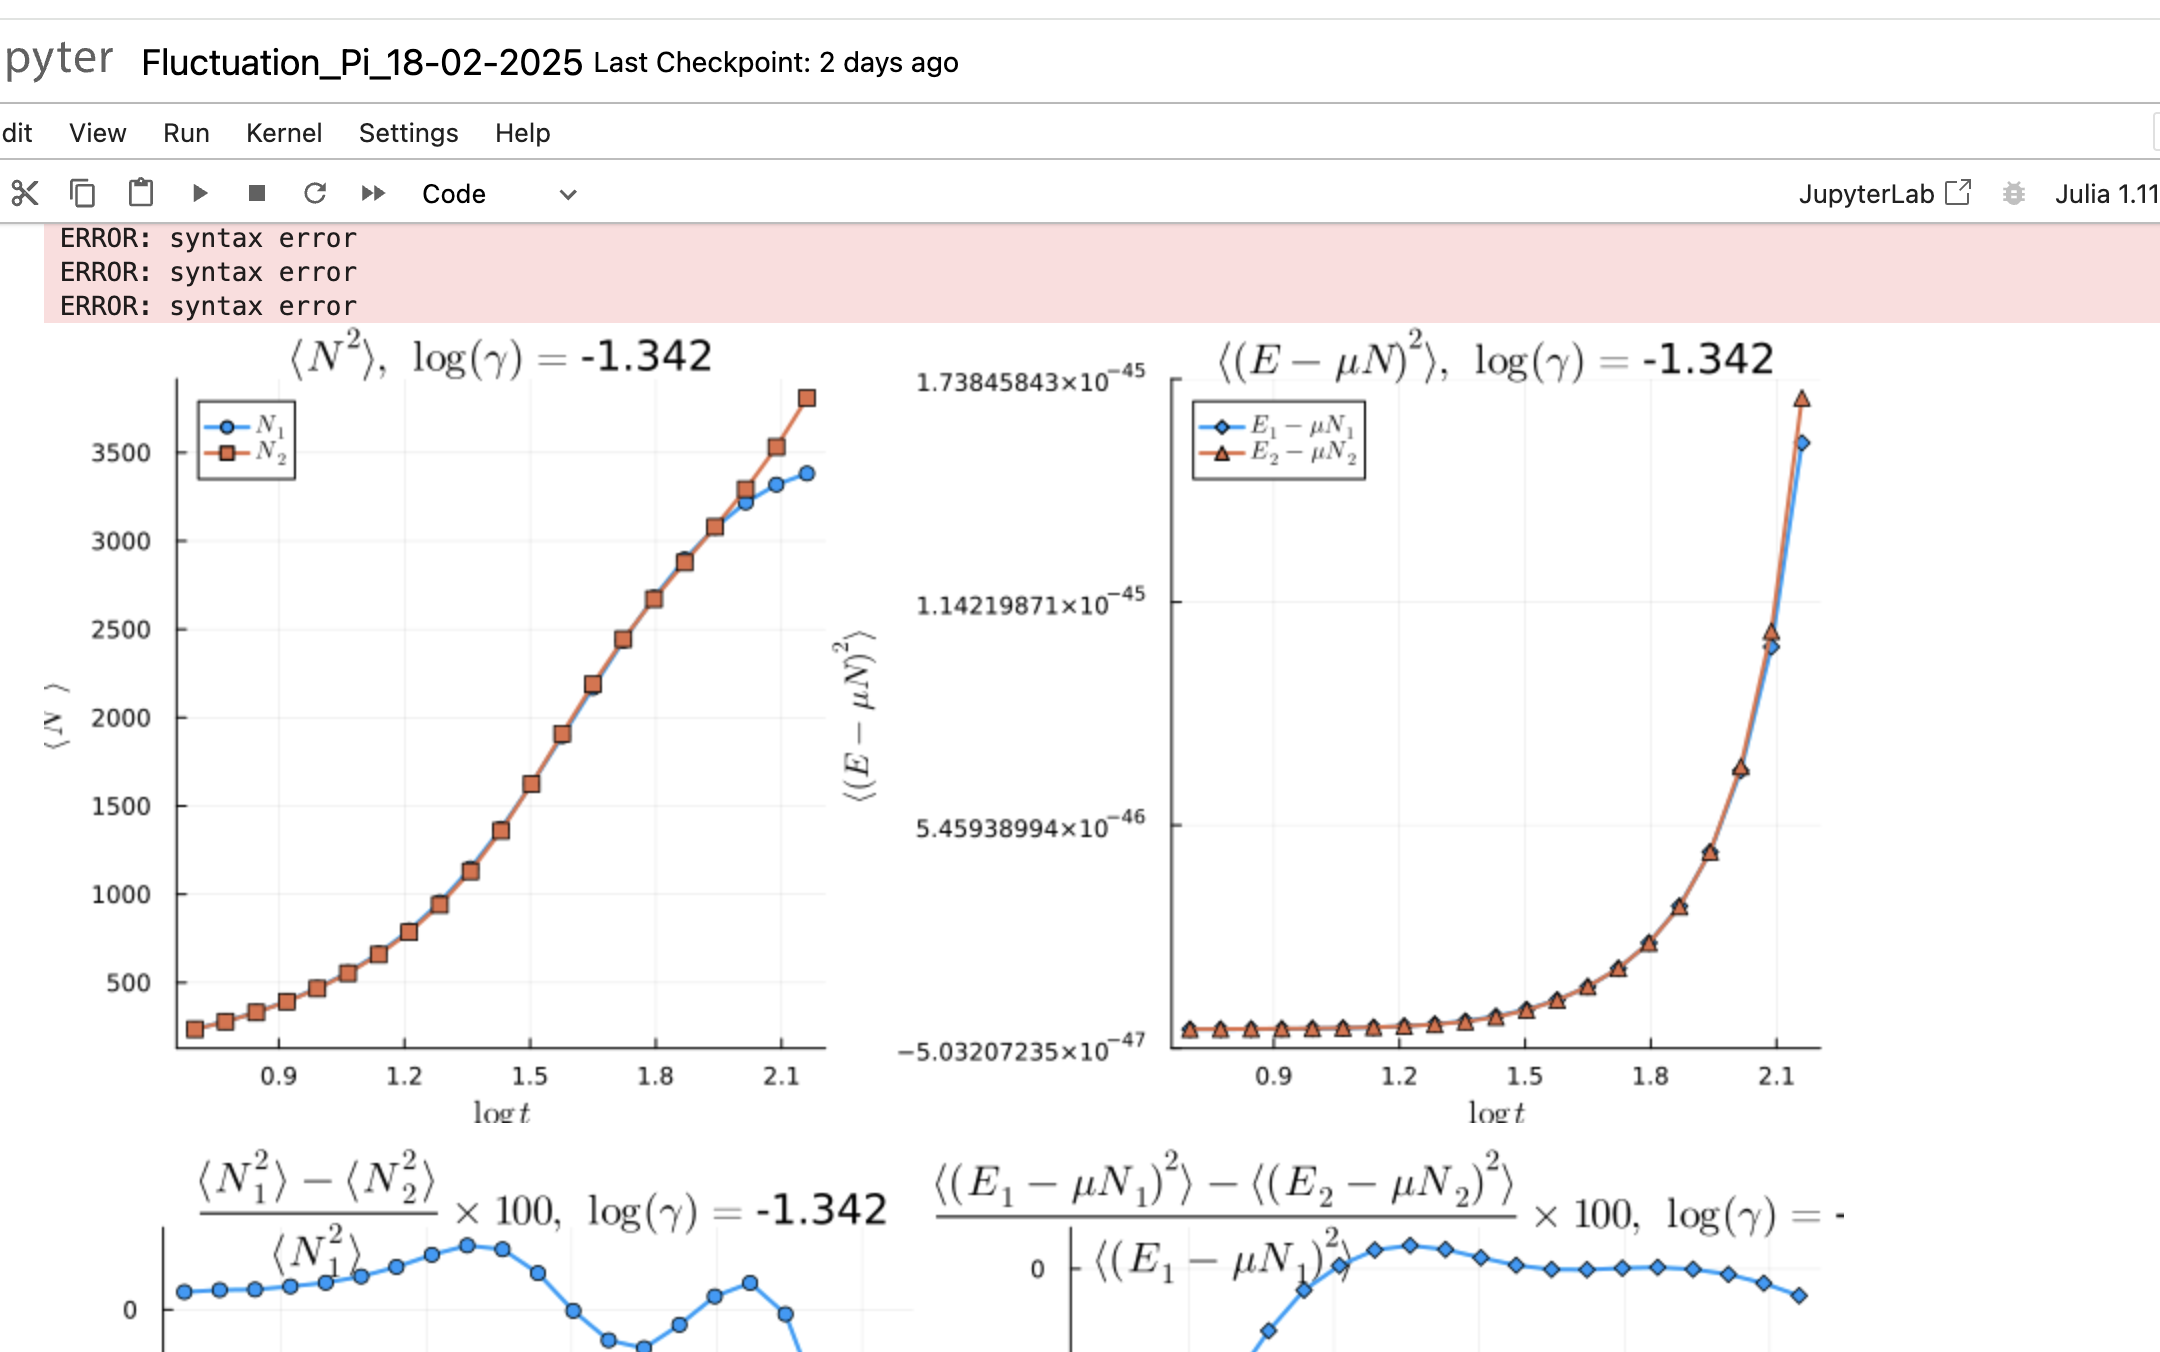
\includegraphics[width=1\textwidth]{Figures/test}

%\begin{aff}
%Donc une a l'ordre un en $\delta \theta (\operator{A}^{(0)})^{-1} %\operator{V}$ 

%\begin{eqnarray*}
%	\langle \delta \Pi ( \theta) \delta \Pi ( \theta') \rangle & = &  ( (\Pi^c_s - \Pi^c)\Pi^c/\Pi^c_s ) ( \theta ) \delta_{\theta, \theta'}/\delta \theta + \mathscr{F}(\theta , \theta' ) ,	
%\end{eqnarray*}

%avec 

%\begin{eqnarray*}
%	\mathscr{F}(\theta , \theta' ) & = & \left [ (\Pi^c_s - \Pi^c )( \theta)  +  (\Pi^c_s - \Pi^c ) ( \theta' )\right ] \frac{\Pi^c}{\Pi^c_s}(\theta)\frac{\Pi^c}{\Pi^c_s}(\theta') \frac{ \Delta( \theta'- \theta )}{ 2 \pi }\\
%	&&  - \left [ (\Pi^c_s - \Pi^c )( \theta)   (\Pi^c_s - \Pi^c ) ( \theta' )\right ] \frac{\Pi^c}{\Pi^c_s}(\theta)\frac{\Pi^c}{\Pi^c_s}(\theta')\int d\theta'' \left (   \frac{ \Pi^c/\Pi^c_s}{\Pi^c_s - \Pi^c} \right )(\theta'') \frac{\Delta(\theta''- \theta)}{2 \pi}\frac{\Delta(\theta''- \theta')}{2 \pi}  	
%\end{eqnarray*}
%\end{aff}



 











%\subsection{Introduction au modèle de gaz de Bose unidimensionnel et Hamiltonien du modèle}
%%Dans ce chapitre, nous nous intéressons aux fluctuations de la distribution de rapidité \( \delta \rho \) autour d'une distribution de référence \( \rho^c \), qui maximise la contribution à la fonction de partition des états, exprimée comme une fonctionnelle de la distribution \( \rho \) : 

La fonction de partition des états, s'exprime comme une fonctionnelle de la distribution \( \rho \) : 

\begin{eqnarray*}
	\Xi & = & \sum_\rho \exp \left( -\mathcal{A}(\rho) \right).
\end{eqnarray*}  

Dans la section {\em \bf Entropie de Yang-Yang} (\ref{??}), l'action \( \mathcal{A}(\rho) \) s'écrit sous la forme :  

\begin{eqnarray*}
	\mathcal{A}(\rho) & \doteq & - L\mathcal{S}_{YY}(\rho) + L\int f(\theta) \rho (\theta) \, d\theta,		
\end{eqnarray*}  

où \( \mathcal{S}_{YY} \) est la fonctionnelle d'entropie de Yang-Yang, définie dans (\ref{??}), et \( f \) est la fonction paramétrant les charges, introduite dans (\ref{??}).  

Dans cette même section {\em \bf Entropie de Yang-Yang} (\ref{??}), nous avons établi un lien entre \( f \) et distribution de référence \( \rho^c \), qui maximise la contribution à la fonction de partition des états .\\

On veux tester si nos experience est décrit pas un GGE. Pour cela nous nous intéressons aux fluctuations de la distribution de rapidité \( \delta \rho \) autour \( \rho^c \).

%Nous poursuivons à présent avec cette définition de l'action de classe $\mathcal{C}^2$ et admetant une distribution critique $\rho^c$ tel que sa différentielle en ce point critique soit nulle $d\mathcal{A}_{\rho^c} = 0 $ (\ref{??}) de sorte que d'aprés la formule de Taylor-Youg %afin de déterminer les fluctuations autour de \( \Pi^c \). Pour cela, nous réécrivons l'action sous la forme :  

Nous poursuivons à présent avec cette définition de l'action de classe $\mathcal{C}^2$ et admetant une distribution critique $\rho^c$ tel que sa différentielle en ce point critique soit nulle $d\mathcal{A}_{\rho^c} = 0 $ (\ref{??}) de sorte que d'aprés la formule de Taylor-Youg %afin de déterminer les fluctuations autour de \( \Pi^c \). Pour cela, nous réécrivons l'action sous la forme :  

\begin{eqnarray*}  
	\mathcal{A}(\rho^c + \delta \rho) & \underset{ \delta \rho \to 0 }{=} & \mathcal{A}(\rho^c)  + \frac{1}{2} \left. \frac{\delta^2 \mathcal{A}}{\delta \rho^2} \right|_{\rho^c} (\delta \rho) + \mathcal{O}((\delta \rho)^3),  
\end{eqnarray*}  

une expression quadratique pour l'action à l'ordre dominant en \( \delta \Pi \) avec $\left. \frac{\delta^2 \mathcal{A}}{\delta \rho^2} \right|_{\rho^c}$ la forme quadratique définie positive (Fig (\ref{fig.fluctu.A})).

\begin{figure}[H]
	\centering 
	\begin{tikzpicture}
		\begin{scope}[shift={(0,0)}]
			\begin{scope}[transform canvas={scale=0.6}]
				% Définition des couleurs avec les codes HTML
\definecolor{colorOne}{HTML}{443E46}
\definecolor{colorTwo}{HTML}{F6DEB8}
\definecolor{colorThree}{HTML}{908CA4}
\definecolor{colorFour}{HTML}{57659E}
\definecolor{colorFive}{HTML}{C57284}
\definecolor{colorSix}{HTML}{FF5B69}

% Raccourcis pour les couleurs
\def\colorOne{colorOne}
\def\colorTwo{colorTwo}
\def\colorThree{colorThree}
\def\colorFour{colorFour}
\def\colorFive{colorFive}
\def\colorSix{colorSix}

\def\colorslide{blue!50!black}



\begin{scope}
	% Tracer une courbe lisse entre des points
	\draw[shift={(0,0)} ,\colorOne]
		(-1 , 0 ) edge [thick,line width=0.8ex , ->,>=triangle 45  , \colorOne] node [pos = 1 , below ]{\huge$\rho$}( 5  , 0 )
	;
	\draw[shift={(0,0)}, color=\colorOne]
		(0, -1.0 ) edge [thick,line width=0.8ex , ->,>=triangle 45  ]node [pos=0.9,left=0.2cm ]{\huge$\mathcal{A}(\rho)$}( 0  , 5 )
	;
	\draw[]
		(2.5, 0.12 ) edge [thick,line width=0.8ex ,\colorThree ]node [pos=1,below  ]{\huge$\rho^c$} (2.5, -0.12 )	
	;
	
	\draw[]
		(2.5, -0.12 ) edge [thick,line width=0.4ex , dashed, \colorThree ] (2.5, 5.5 )
		(1.5, 1 ) edge [thick,line width=0.4ex , <->,>=triangle 45  , \colorThree ] (3.5, 1 )
		(-0.3,1) edge [thick,line width=0.4ex  , \colorThree ] node [pos=0,left ]{\huge$\mathcal{A}(\rho^c)$} (0.3, 1 )	
	;
    \draw[thick, line width=0.8ex , \colorFour] plot[smooth, tension=0.7] coordinates {
        (1, 5) (1.6 , 3 ) (2.5, 1) (3.5 , 3 )  (4, 5)
    };		
	
\end{scope}

	
			
			\end{scope}
			
			\draw[color = red , scale = 0.5 , draw = none  ] (-2 , -1) rectangle (5, 6) ; 	
		\end{scope}
		
		\begin{scope}[shift={(19,-1)}]
			\begin{scope}[transform canvas={scale=0.6}]
				% Définition des couleurs avec les codes HTML
\definecolor{colorOne}{HTML}{443E46}
\definecolor{colorTwo}{HTML}{F6DEB8}
\definecolor{colorThree}{HTML}{908CA4}
\definecolor{colorFour}{HTML}{57659E}
\definecolor{colorFive}{HTML}{C57284}
\definecolor{colorSix}{HTML}{FF5B69}

% Raccourcis pour les couleurs
\def\colorOne{colorOne}
\def\colorTwo{colorTwo}
\def\colorThree{colorThree}
\def\colorFour{colorFour}
\def\colorFive{colorFive}
\def\colorSix{colorSix}

\def\colorslide{blue!50!black}

\def\Occupation{
	\def\traitx{0.3}
	\def\traity{0.5}
	\draw[shift={(0,0)}]
		(-13.5 , 0 ) edge [thick,line width=0.8ex ]( -3.2  , 0 )
		( -3.2 - \traitx  , 0 - \traity ) edge [thick,line width=0.8ex ]( -3.2 + \traitx  , 0 + \traity  )
		( -2.8 - \traitx  , 0 - \traity ) edge [thick,line width=0.8ex ]( -2.8 + \traitx  , 0 + \traity  )
		(-2.8 , 0 ) edge [thick,line width=0.8ex ](2.8  , 0 )
		( 2.8 - \traitx  , 0 - \traity ) edge [thick,line width=0.8ex ]( 2.8 + \traitx  , 0 + \traity  )
		( 3.2 - \traitx  , 0 - \traity ) edge [thick,line width=0.8ex ]( 3.2 + \traitx  , 0 + \traity  )
		(3.2, 0 ) edge [thick,line width=0.8ex,->,>=triangle 45 , color = black ]node [pos=1.01,below  ]{\huge$\theta$}	( 13  , 0 )
	;
	\draw[shift={(0,0)}, color=\colorOne]
		(-10.5 , -1.5 ) edge [thick,line width=0.8ex , ->,>=triangle 45  ]( -10.5  , 4.5 )
	;
		
	\foreach \r in {1 , ... , 3 } {
%		\draw[
%		decoration={
%		markings,
%    	mark connection node=my node,
%    	mark=at position 0 with{\node [blue,transform shape] (my node) {\large \r};}},
%		color=gray, thick, 
%		line width=0.5ex] decorate { 
%            (-11.0, \r) -- (-10.1, \r )}
%        ;
        \draw[
			color=\colorOne,
			] 
            (-11.0, \r) edge[color=\colorThree , thick,line width=0.5ex] node [pos=-0.5 ]{\large\color{\colorFour} $\frac{\r}{\delta \theta}$ } (-10.3, \r )
        	;
	
	}
	

	
	% Graduation abcsisse 
	% Définitions des listes
% Definitions of the lists
\def\listetuple{-9/\theta_{1}, -8/\theta_{2} , -5/\theta_{3} , -2/\theta_{a-1} , 0/\theta_{a} , 1/\theta_{a+1} , 2/\theta_{a+2} ,  5/\theta_{N-4} , 7/\theta_{N-3},8/\theta_{N-1},9/\theta_{N} }
\def\listetrais{-12 , -11, -10, -9 , -8 , -7 ,  -6 , -5, -4.5,-4, -2 , -1, 0 , 0.5, 1, 2, 4 , 5 ,  6 , 7 , 8 ,8.5, 9 ,  10 , 11, 12 }

% Loop over listetrais
\foreach \r in \listetrais {
    % Initialize found variable to zero
    % Initialize found variable to zero
    %\pgfmathsetmacro\found{0}
    \global\def\found{0}
    \xdef\nomtheta{}
    
    % Check if \r is in listetuple
    \foreach \x/\y in \listetuple { 
        \ifdim \r pt=\x pt % If \r matches any \x in listetuple
            \global\def\found{1} ;
            \xdef\nomtheta{\y} % Set \nomtheta to the corresponding \y
            %\pgfmathsetmacro\found{1} % Set found to 1            
            %\global\pgfmathsetmacro\found{1}
        \fi
    }
    
    %\node [circle, draw, red] (A) at (\r, 2) {\found , $\nomtheta$};
    
    % Draw the line and display \nomtheta if found
    \ifnum\found=1
        \draw[color=\colorOne, thick, line width=0.5ex] 
            (\r, -0.3) -- (\r, 0.3) node[red , pos=-0.5] {\large $\nomtheta$};
         \filldraw[line width=0.5ex, color=\colorSix, outer color=\colorSix, inner color=\colorSix] 
            (\r, 0) circle (4pt);
    \else 
        % Draw without \nomtheta and add a blue circle if not found
        \draw[color=\colorOne, thick, line width=0.5ex] 
            (\r, -0.3) -- (\r, 0.3);
        \filldraw[line width=0.5ex, color=\colorSix, outer color=\colorTwo, inner color=\colorTwo] 
            (\r, 0) circle (4pt); 
    \fi
}

\def\listetrais{-9.5/\theta_{i-1}/2/3, -6.5/\theta_{i}/1/4  ,   -1.5/\theta_{j}/2/4 , 1.5/\theta_{j+1}/-1/3 , 3.5/\theta_{\ell-1}/1/3 , 6.5/\theta_{\ell}/3/4 , 9.5/\theta(\theta_{\ell+1})/-1/3 };



\foreach \r/\nomx/\y/\ys in \listetrais {
	\draw[
		decoration={
		markings,
    	mark connection node=my node,
    	mark=at position .5 with{\node [blue,transform shape] (my node) {\large \color{\colorFour} $\nomx$};}},
		color=\colorThree , thick, 
		line width=0.5ex] decorate { 
            (\r, 0.12) -- (\r, -1.2)}
        ;
     
     \ifdim \y pt > -1 pt 
     	\draw[
			decoration={
			markings,
    		mark connection node=my node,
    		mark=at position .5 with{\node [blue,transform shape] (my node) {\large \color{\colorFour} $\Pi(\nomx) $};}},
			color=\colorThree, thick, 
			line width=0.5ex] decorate { 
            (\r, \y) -- (\r +3, \y)}
        ;
        \draw[
			decoration={
			markings,
    		mark connection node=my node,
    		mark=at position .5 with{\node [blue,transform shape] (my node) {\large \color{\colorFive} $\Pi_s(\nomx) $};}},
			color=\colorFive, thick, 
			line width=0.5ex] decorate { 
            (\r, \ys) -- (\r +3, \ys)}
        ;
     \fi 
     \ifdim \r pt= -1.5 pt
     	\draw[
     		decoration={
			markings,
    		mark connection node=my node,
    		mark=at position .5 with{\node [blue,transform shape] (my node) {\large \color{\colorFour}  $\delta \theta $};},
    		%mark=at position 0.1  with {\arrow[blue, line width=0.5ex]{<}},
    		%mark=at position 1  with {\arrow[blue, line width=0.5ex]{>}}
    		},
        	color=\colorThree,
        	thick,
        	line width=0.5ex,
        	%arrows={Computer Modern Rightarrow[line cap=round]-Computer Modern Rightarrow[line cap=round]}
   			](\r, -1.2) edge[arrows={Computer Modern Rightarrow[line cap=round]-}] (\r + 0.4, -1.2)decorate {
    		(\r, -1.2) -- (\r + 3, -1.2)}(\r + 2, -1.2) edge[arrows={-Computer Modern Rightarrow[line cap=round]}] (\r + 3, -1.2)
    		;
    \fi
			
	
}


			
}


\begin{scope}
	%\draw[help lines , width=1.5ex] (-8,-3) grid (8,3);\draw[help lines ,width=0.5ex , opacity = 0.5] (-3,-3) grid[step=0.1] (3,3));
	
	%\draw[help lines] 
	%	(-3,-3) edge[width=1.5ex] grid (3,3)	
	%	(-3,-3) edge[width=0.5ex , opacity = 0.5] grid (3,3)	
	%;
	\begin{scope}[shift={(0,1)},rotate=0,opacity=1,color=black]
		\Occupation	
		
		%\node[anchor=east, font=\bfseries] at (-11, 0) {\color{red}\large (T = 0 )} ;	
	\end{scope}
	
	
	
	
	\begin{scope}[shift={(-10.5,7)},rotate=0,opacity=1,color=black]
	
	\begin{scope}[shift={(-0,0)},rotate=0,opacity=1,color=black]
	
		\draw[shift={(0,0)} ,line width=1ex,rounded corners = 1ex,color=\colorOne , opacity =1 ,fill=\colorOne!00 , pattern={north east lines} , pattern color=\colorOne!00 ]
			(0 , -1 ) rectangle (5,1)
		;
		

		\begin{scope}[shift={(0.5,0.5)}]
			\draw[color=\colorOne, thick, line width=0.5ex] 
            (0, -0.3) -- (0, 0.3) ;
            \filldraw[line width=0.5ex, color=\colorSix, outer color=\colorSix, inner color=\colorSix] 
            (0, 0) circle (4pt);
            
            \node[anchor=west, font=\bfseries] at (0.2, 0) {\color{\colorSix}\large : quasi-particule};
		\end{scope}
		
		\begin{scope}[shift={(0.5,-0.5)}]
			\draw[color=\colorOne, thick, line width=0.5ex] 
            (0, -0.3) -- (0, 0.3) ;
            \filldraw[line width=0.5ex, color=\colorSix, outer color=\colorTwo, inner color=\colorTwo] 
            (0, 0) circle (4pt);
            
            \node[anchor=west, font=\bfseries] at (0.2, 0) {\color{\colorSix}\large : hole};
		\end{scope}

	\end{scope}
	
	\begin{scope}[shift={(6,0)},rotate=0,opacity=1,color=black]	
		
		\draw[shift={(0,0)} ,line width=1ex,rounded corners = 1ex,color=\colorOne , opacity =1 ,fill=\colorOne!00 , pattern={north east lines} , pattern color=\colorOne!00 ]
			(0 , -1 ) rectangle (7.5,1)
		;
		
		\node[anchor=west] at (0.5, 0.5) {\color{\colorFour}\large $\Pi$ };\node[anchor=west, font=\bfseries] at (1, 0.5) {\color{\colorFour}\large : quasi-particule distribution};
		
		\node[anchor=west] at (0.5, -0.5) {\color{\colorFour}\large $\Pi_h$ };\node[anchor=west, font=\bfseries] at (1, -0.5) {\color{\colorFour}\large  : hole distribution};
		
	\end{scope}
	
	\begin{scope}[shift={(14.5,0)},rotate=0,opacity=1,color=black]	
		
		\draw[shift={(0,0)} ,line width=1ex,rounded corners = 1ex,color=\colorOne , opacity =1 ,fill=\colorOne!00 , pattern={north east lines} , pattern color=\colorOne!00 ]
			(0 , -0.5 ) rectangle (7.0,0.5)
		;
		
		\node[anchor=west] at (0.2, 0) {\color{\colorFour}\large ${\color{\colorFive}\Pi_s} = \Pi + \Pi_h $ } node[anchor=west , font=\bfseries] at (3.1 , 0 )  {\color{\colorFour}\large {\color{\colorFive} : density of states}};
		
	\end{scope}
	
	
	\end{scope}


		
	
\end{scope}

	
			
			\end{scope}
			\begin{scope}[scale=1]
				\draw[color = red , scale = 1 , draw = none  ] (-1 , -1) rectangle (5, 5) ; 
			\end{scope}	
		\end{scope}

		
				
			
	\end{tikzpicture}	
	\captionsetup{skip=10pt} % Ajoute de l’espace après la légende
	\label{fig.fluctu.A}
\end{figure}


On discrétise l'axe des rapidités en  petite cellule de rapidité $[\theta, \theta+\delta\theta]$, qui contient $L\rho(\theta) \delta \theta$ rapidités. 
	



Avec ces petites tranches, la forme quadratique s’écrit :

\begin{eqnarray*}
    \left. \frac{\delta^2 \mathcal{A}}{{\delta \rho}^2} \right|_{\rho^c}(\delta \rho ) &=&  \sum_{a,b \mid \text{tranche}}  
    \delta \rho(\theta_a)  \frac{\partial^2 \mathcal{A}}{\partial \delta \rho(\theta_a) \partial \delta \rho(\theta_b) } (\rho^c)  \delta \rho(\theta_b).
\end{eqnarray*}
Les fluctuations s’écrivent donc :

\begin{eqnarray*}
    \langle \delta \rho ( \theta) \delta \rho ( \theta') \rangle &=&  
    \frac{ \int d\delta \rho \, \delta \rho(\theta) \delta \rho ( \theta') 
    \exp \left( - \frac{1}{2} \sum_{a,b \mid \text{tranche}}  
    \delta \rho(\theta_a) \frac{\partial^2 \mathcal{A}}{\partial \delta \rho(\theta_a) \partial \delta \rho(\theta_b) } (\rho^c)  \delta \rho(\theta_b) \right) }
    { \int d\delta \Pi  
    \exp \left( - \frac{1}{2} \sum_{a,b \mid \text{tranche}}  
    \delta \rho(\theta_a) \frac{\partial^2 \mathcal{A}}{\partial \delta \rho(\theta_a) \partial \delta \rho(\theta_b) } (\rho^c)  \delta \rho(\theta_b) \right) } \\
    &=& \left( \mathbf{A}^{-1} \right)_{\theta , \theta'}
\end{eqnarray*}


\begin{aff}

\begin{eqnarray*}
	\langle \delta \rho ( \theta) \delta \rho ( \theta') \rangle &=& 	\left( \mathbf{A}^{-1} \right)_{\theta , \theta'}
\end{eqnarray*}

	
avec la  {\em matrice hessienne} $\mathbf{A}_{\theta , \theta'} \equiv \frac{\partial^2 \mathcal{A}}{\partial \delta \rho(\theta) \partial \delta \rho(\theta') }(\rho^c)$, au point critique/ qui maximise la probabilité  $\rho^c=\rho^c_s \nu^c $, s'écrit

\begin{eqnarray*}
	\operator{A} & = & \operator{A}^{(0)} + \delta \theta \operator{V}
\end{eqnarray*}

avec 

\begin{eqnarray*}
	A^{(0)}_{\theta , \theta'}  & = &  L\delta \theta \left ( \frac{ 1}{\rho^c_s ( 1  - \nu^c ) \nu^c } \right )(\theta)    \delta({\theta - \theta '})	,\\
	V_{\theta , \theta'}  &= & L \delta \theta \left \{ - \left [ \left ( \frac{1}{\rho^c_s( 1 - \nu^c) } \right ) ( \theta)  +  \left ( \frac{1}{\rho^c_s( 1 - \nu^c) } \right ) ( \theta' )\right ] \frac{ \Delta( \theta'- \theta )}{ 2 \pi } + \int d\theta''  \left ( \frac{\nu^c}{\rho^c_s( 1 - \nu^c) } \right )(\theta'') \frac{\Delta(\theta''- \theta)}{2 \pi}\frac{\Delta(\theta''- \theta')}{2 \pi}   \right \} 	
\end{eqnarray*}

\end{aff}

\subsection{Testes}

\begin{eqnarray*}
	\Delta_{\operator{\mathcal{N}}}^2  & = &  \frac{1}{\beta} \left . \frac{\partial \langle \operator{\mathcal{N}} \rangle}{\partial \mu} \right )_T \\
	\Delta_{\operator{\mathcal{E}}-\mu \operator{\mathcal{N}}}^2  & = &  - \left . \frac{\partial \langle \operator{\mathcal{E}}-\mu \operator{\mathcal{N}} \rangle}{\partial \beta} \right )_\mu 
\end{eqnarray*}

et 

\begin{eqnarray*}
	\Delta_{\operator{\mathcal{N}}}^2  &= & L^2 \int d\theta_a \int d \theta_b \, \langle \delta \rho(\theta_a) \delta \rho(\theta_b) \rangle \\
	\Delta_{\operator{\mathcal{E}}-\mu \operator{\mathcal{N}}}^2  & = & L^2 \int d\theta_a \int d \theta_b \, \left ( - \mu + \frac{1}2 m \theta_a^2  \right  )\left ( - \mu + \frac{1}2 m \theta_b^2  \right  )  \langle \delta \rho(\theta_a) \delta \rho(\theta_b) \rangle
\end{eqnarray*}

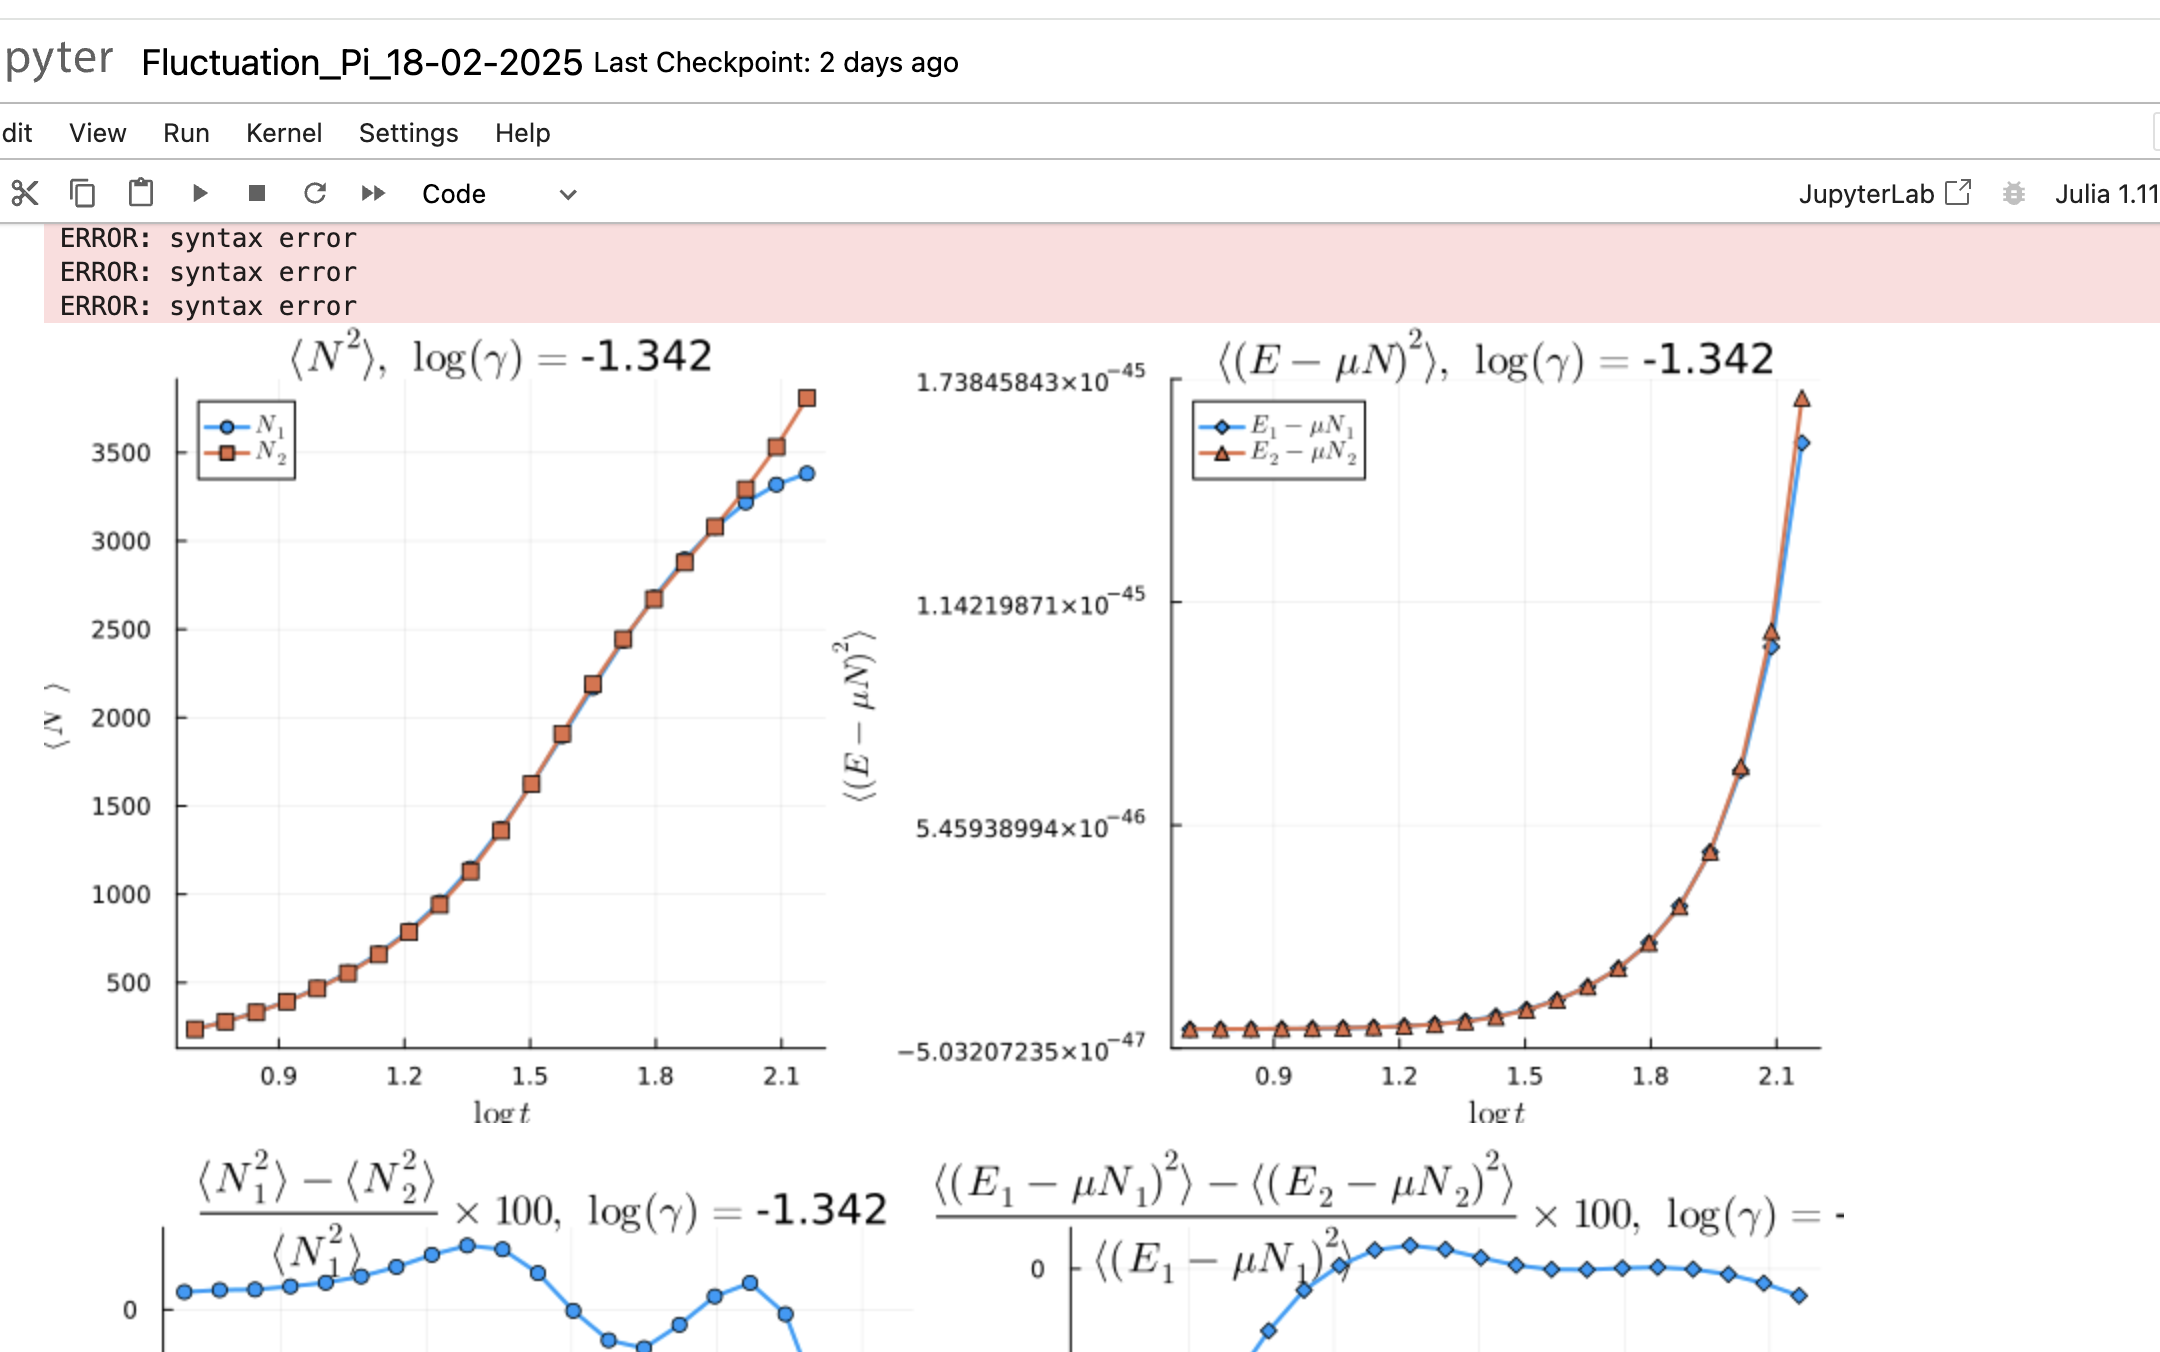
\includegraphics[width=1\textwidth]{Figures/test}

%\begin{aff}
%Donc une a l'ordre un en $\delta \theta (\operator{A}^{(0)})^{-1} %\operator{V}$ 

%\begin{eqnarray*}
%	\langle \delta \Pi ( \theta) \delta \Pi ( \theta') \rangle & = &  ( (\Pi^c_s - \Pi^c)\Pi^c/\Pi^c_s ) ( \theta ) \delta_{\theta, \theta'}/\delta \theta + \mathscr{F}(\theta , \theta' ) ,	
%\end{eqnarray*}

%avec 

%\begin{eqnarray*}
%	\mathscr{F}(\theta , \theta' ) & = & \left [ (\Pi^c_s - \Pi^c )( \theta)  +  (\Pi^c_s - \Pi^c ) ( \theta' )\right ] \frac{\Pi^c}{\Pi^c_s}(\theta)\frac{\Pi^c}{\Pi^c_s}(\theta') \frac{ \Delta( \theta'- \theta )}{ 2 \pi }\\
%	&&  - \left [ (\Pi^c_s - \Pi^c )( \theta)   (\Pi^c_s - \Pi^c ) ( \theta' )\right ] \frac{\Pi^c}{\Pi^c_s}(\theta)\frac{\Pi^c}{\Pi^c_s}(\theta')\int d\theta'' \left (   \frac{ \Pi^c/\Pi^c_s}{\Pi^c_s - \Pi^c} \right )(\theta'') \frac{\Delta(\theta''- \theta)}{2 \pi}\frac{\Delta(\theta''- \theta')}{2 \pi}  	
%\end{eqnarray*}
%\end{aff}



 








%\subsection{Hamiltonien du modèle}
%%Dans ce chapitre, nous nous intéressons aux fluctuations de la distribution de rapidité \( \delta \rho \) autour d'une distribution de référence \( \rho^c \), qui maximise la contribution à la fonction de partition des états, exprimée comme une fonctionnelle de la distribution \( \rho \) : 

La fonction de partition des états, s'exprime comme une fonctionnelle de la distribution \( \rho \) : 

\begin{eqnarray*}
	\Xi & = & \sum_\rho \exp \left( -\mathcal{A}(\rho) \right).
\end{eqnarray*}  

Dans la section {\em \bf Entropie de Yang-Yang} (\ref{??}), l'action \( \mathcal{A}(\rho) \) s'écrit sous la forme :  

\begin{eqnarray*}
	\mathcal{A}(\rho) & \doteq & - L\mathcal{S}_{YY}(\rho) + L\int f(\theta) \rho (\theta) \, d\theta,		
\end{eqnarray*}  

où \( \mathcal{S}_{YY} \) est la fonctionnelle d'entropie de Yang-Yang, définie dans (\ref{??}), et \( f \) est la fonction paramétrant les charges, introduite dans (\ref{??}).  

Dans cette même section {\em \bf Entropie de Yang-Yang} (\ref{??}), nous avons établi un lien entre \( f \) et distribution de référence \( \rho^c \), qui maximise la contribution à la fonction de partition des états .\\

On veux tester si nos experience est décrit pas un GGE. Pour cela nous nous intéressons aux fluctuations de la distribution de rapidité \( \delta \rho \) autour \( \rho^c \).

%Nous poursuivons à présent avec cette définition de l'action de classe $\mathcal{C}^2$ et admetant une distribution critique $\rho^c$ tel que sa différentielle en ce point critique soit nulle $d\mathcal{A}_{\rho^c} = 0 $ (\ref{??}) de sorte que d'aprés la formule de Taylor-Youg %afin de déterminer les fluctuations autour de \( \Pi^c \). Pour cela, nous réécrivons l'action sous la forme :  

Nous poursuivons à présent avec cette définition de l'action de classe $\mathcal{C}^2$ et admetant une distribution critique $\rho^c$ tel que sa différentielle en ce point critique soit nulle $d\mathcal{A}_{\rho^c} = 0 $ (\ref{??}) de sorte que d'aprés la formule de Taylor-Youg %afin de déterminer les fluctuations autour de \( \Pi^c \). Pour cela, nous réécrivons l'action sous la forme :  

\begin{eqnarray*}  
	\mathcal{A}(\rho^c + \delta \rho) & \underset{ \delta \rho \to 0 }{=} & \mathcal{A}(\rho^c)  + \frac{1}{2} \left. \frac{\delta^2 \mathcal{A}}{\delta \rho^2} \right|_{\rho^c} (\delta \rho) + \mathcal{O}((\delta \rho)^3),  
\end{eqnarray*}  

une expression quadratique pour l'action à l'ordre dominant en \( \delta \Pi \) avec $\left. \frac{\delta^2 \mathcal{A}}{\delta \rho^2} \right|_{\rho^c}$ la forme quadratique définie positive (Fig (\ref{fig.fluctu.A})).

\begin{figure}[H]
	\centering 
	\begin{tikzpicture}
		\begin{scope}[shift={(0,0)}]
			\begin{scope}[transform canvas={scale=0.6}]
				% Définition des couleurs avec les codes HTML
\definecolor{colorOne}{HTML}{443E46}
\definecolor{colorTwo}{HTML}{F6DEB8}
\definecolor{colorThree}{HTML}{908CA4}
\definecolor{colorFour}{HTML}{57659E}
\definecolor{colorFive}{HTML}{C57284}
\definecolor{colorSix}{HTML}{FF5B69}

% Raccourcis pour les couleurs
\def\colorOne{colorOne}
\def\colorTwo{colorTwo}
\def\colorThree{colorThree}
\def\colorFour{colorFour}
\def\colorFive{colorFive}
\def\colorSix{colorSix}

\def\colorslide{blue!50!black}



\begin{scope}
	% Tracer une courbe lisse entre des points
	\draw[shift={(0,0)} ,\colorOne]
		(-1 , 0 ) edge [thick,line width=0.8ex , ->,>=triangle 45  , \colorOne] node [pos = 1 , below ]{\huge$\rho$}( 5  , 0 )
	;
	\draw[shift={(0,0)}, color=\colorOne]
		(0, -1.0 ) edge [thick,line width=0.8ex , ->,>=triangle 45  ]node [pos=0.9,left=0.2cm ]{\huge$\mathcal{A}(\rho)$}( 0  , 5 )
	;
	\draw[]
		(2.5, 0.12 ) edge [thick,line width=0.8ex ,\colorThree ]node [pos=1,below  ]{\huge$\rho^c$} (2.5, -0.12 )	
	;
	
	\draw[]
		(2.5, -0.12 ) edge [thick,line width=0.4ex , dashed, \colorThree ] (2.5, 5.5 )
		(1.5, 1 ) edge [thick,line width=0.4ex , <->,>=triangle 45  , \colorThree ] (3.5, 1 )
		(-0.3,1) edge [thick,line width=0.4ex  , \colorThree ] node [pos=0,left ]{\huge$\mathcal{A}(\rho^c)$} (0.3, 1 )	
	;
    \draw[thick, line width=0.8ex , \colorFour] plot[smooth, tension=0.7] coordinates {
        (1, 5) (1.6 , 3 ) (2.5, 1) (3.5 , 3 )  (4, 5)
    };		
	
\end{scope}

	
			
			\end{scope}
			
			\draw[color = red , scale = 0.5 , draw = none  ] (-2 , -1) rectangle (5, 6) ; 	
		\end{scope}
		
		\begin{scope}[shift={(19,-1)}]
			\begin{scope}[transform canvas={scale=0.6}]
				% Définition des couleurs avec les codes HTML
\definecolor{colorOne}{HTML}{443E46}
\definecolor{colorTwo}{HTML}{F6DEB8}
\definecolor{colorThree}{HTML}{908CA4}
\definecolor{colorFour}{HTML}{57659E}
\definecolor{colorFive}{HTML}{C57284}
\definecolor{colorSix}{HTML}{FF5B69}

% Raccourcis pour les couleurs
\def\colorOne{colorOne}
\def\colorTwo{colorTwo}
\def\colorThree{colorThree}
\def\colorFour{colorFour}
\def\colorFive{colorFive}
\def\colorSix{colorSix}

\def\colorslide{blue!50!black}

\def\Occupation{
	\def\traitx{0.3}
	\def\traity{0.5}
	\draw[shift={(0,0)}]
		(-13.5 , 0 ) edge [thick,line width=0.8ex ]( -3.2  , 0 )
		( -3.2 - \traitx  , 0 - \traity ) edge [thick,line width=0.8ex ]( -3.2 + \traitx  , 0 + \traity  )
		( -2.8 - \traitx  , 0 - \traity ) edge [thick,line width=0.8ex ]( -2.8 + \traitx  , 0 + \traity  )
		(-2.8 , 0 ) edge [thick,line width=0.8ex ](2.8  , 0 )
		( 2.8 - \traitx  , 0 - \traity ) edge [thick,line width=0.8ex ]( 2.8 + \traitx  , 0 + \traity  )
		( 3.2 - \traitx  , 0 - \traity ) edge [thick,line width=0.8ex ]( 3.2 + \traitx  , 0 + \traity  )
		(3.2, 0 ) edge [thick,line width=0.8ex,->,>=triangle 45 , color = black ]node [pos=1.01,below  ]{\huge$\theta$}	( 13  , 0 )
	;
	\draw[shift={(0,0)}, color=\colorOne]
		(-10.5 , -1.5 ) edge [thick,line width=0.8ex , ->,>=triangle 45  ]( -10.5  , 4.5 )
	;
		
	\foreach \r in {1 , ... , 3 } {
%		\draw[
%		decoration={
%		markings,
%    	mark connection node=my node,
%    	mark=at position 0 with{\node [blue,transform shape] (my node) {\large \r};}},
%		color=gray, thick, 
%		line width=0.5ex] decorate { 
%            (-11.0, \r) -- (-10.1, \r )}
%        ;
        \draw[
			color=\colorOne,
			] 
            (-11.0, \r) edge[color=\colorThree , thick,line width=0.5ex] node [pos=-0.5 ]{\large\color{\colorFour} $\frac{\r}{\delta \theta}$ } (-10.3, \r )
        	;
	
	}
	

	
	% Graduation abcsisse 
	% Définitions des listes
% Definitions of the lists
\def\listetuple{-9/\theta_{1}, -8/\theta_{2} , -5/\theta_{3} , -2/\theta_{a-1} , 0/\theta_{a} , 1/\theta_{a+1} , 2/\theta_{a+2} ,  5/\theta_{N-4} , 7/\theta_{N-3},8/\theta_{N-1},9/\theta_{N} }
\def\listetrais{-12 , -11, -10, -9 , -8 , -7 ,  -6 , -5, -4.5,-4, -2 , -1, 0 , 0.5, 1, 2, 4 , 5 ,  6 , 7 , 8 ,8.5, 9 ,  10 , 11, 12 }

% Loop over listetrais
\foreach \r in \listetrais {
    % Initialize found variable to zero
    % Initialize found variable to zero
    %\pgfmathsetmacro\found{0}
    \global\def\found{0}
    \xdef\nomtheta{}
    
    % Check if \r is in listetuple
    \foreach \x/\y in \listetuple { 
        \ifdim \r pt=\x pt % If \r matches any \x in listetuple
            \global\def\found{1} ;
            \xdef\nomtheta{\y} % Set \nomtheta to the corresponding \y
            %\pgfmathsetmacro\found{1} % Set found to 1            
            %\global\pgfmathsetmacro\found{1}
        \fi
    }
    
    %\node [circle, draw, red] (A) at (\r, 2) {\found , $\nomtheta$};
    
    % Draw the line and display \nomtheta if found
    \ifnum\found=1
        \draw[color=\colorOne, thick, line width=0.5ex] 
            (\r, -0.3) -- (\r, 0.3) node[red , pos=-0.5] {\large $\nomtheta$};
         \filldraw[line width=0.5ex, color=\colorSix, outer color=\colorSix, inner color=\colorSix] 
            (\r, 0) circle (4pt);
    \else 
        % Draw without \nomtheta and add a blue circle if not found
        \draw[color=\colorOne, thick, line width=0.5ex] 
            (\r, -0.3) -- (\r, 0.3);
        \filldraw[line width=0.5ex, color=\colorSix, outer color=\colorTwo, inner color=\colorTwo] 
            (\r, 0) circle (4pt); 
    \fi
}

\def\listetrais{-9.5/\theta_{i-1}/2/3, -6.5/\theta_{i}/1/4  ,   -1.5/\theta_{j}/2/4 , 1.5/\theta_{j+1}/-1/3 , 3.5/\theta_{\ell-1}/1/3 , 6.5/\theta_{\ell}/3/4 , 9.5/\theta(\theta_{\ell+1})/-1/3 };



\foreach \r/\nomx/\y/\ys in \listetrais {
	\draw[
		decoration={
		markings,
    	mark connection node=my node,
    	mark=at position .5 with{\node [blue,transform shape] (my node) {\large \color{\colorFour} $\nomx$};}},
		color=\colorThree , thick, 
		line width=0.5ex] decorate { 
            (\r, 0.12) -- (\r, -1.2)}
        ;
     
     \ifdim \y pt > -1 pt 
     	\draw[
			decoration={
			markings,
    		mark connection node=my node,
    		mark=at position .5 with{\node [blue,transform shape] (my node) {\large \color{\colorFour} $\Pi(\nomx) $};}},
			color=\colorThree, thick, 
			line width=0.5ex] decorate { 
            (\r, \y) -- (\r +3, \y)}
        ;
        \draw[
			decoration={
			markings,
    		mark connection node=my node,
    		mark=at position .5 with{\node [blue,transform shape] (my node) {\large \color{\colorFive} $\Pi_s(\nomx) $};}},
			color=\colorFive, thick, 
			line width=0.5ex] decorate { 
            (\r, \ys) -- (\r +3, \ys)}
        ;
     \fi 
     \ifdim \r pt= -1.5 pt
     	\draw[
     		decoration={
			markings,
    		mark connection node=my node,
    		mark=at position .5 with{\node [blue,transform shape] (my node) {\large \color{\colorFour}  $\delta \theta $};},
    		%mark=at position 0.1  with {\arrow[blue, line width=0.5ex]{<}},
    		%mark=at position 1  with {\arrow[blue, line width=0.5ex]{>}}
    		},
        	color=\colorThree,
        	thick,
        	line width=0.5ex,
        	%arrows={Computer Modern Rightarrow[line cap=round]-Computer Modern Rightarrow[line cap=round]}
   			](\r, -1.2) edge[arrows={Computer Modern Rightarrow[line cap=round]-}] (\r + 0.4, -1.2)decorate {
    		(\r, -1.2) -- (\r + 3, -1.2)}(\r + 2, -1.2) edge[arrows={-Computer Modern Rightarrow[line cap=round]}] (\r + 3, -1.2)
    		;
    \fi
			
	
}


			
}


\begin{scope}
	%\draw[help lines , width=1.5ex] (-8,-3) grid (8,3);\draw[help lines ,width=0.5ex , opacity = 0.5] (-3,-3) grid[step=0.1] (3,3));
	
	%\draw[help lines] 
	%	(-3,-3) edge[width=1.5ex] grid (3,3)	
	%	(-3,-3) edge[width=0.5ex , opacity = 0.5] grid (3,3)	
	%;
	\begin{scope}[shift={(0,1)},rotate=0,opacity=1,color=black]
		\Occupation	
		
		%\node[anchor=east, font=\bfseries] at (-11, 0) {\color{red}\large (T = 0 )} ;	
	\end{scope}
	
	
	
	
	\begin{scope}[shift={(-10.5,7)},rotate=0,opacity=1,color=black]
	
	\begin{scope}[shift={(-0,0)},rotate=0,opacity=1,color=black]
	
		\draw[shift={(0,0)} ,line width=1ex,rounded corners = 1ex,color=\colorOne , opacity =1 ,fill=\colorOne!00 , pattern={north east lines} , pattern color=\colorOne!00 ]
			(0 , -1 ) rectangle (5,1)
		;
		

		\begin{scope}[shift={(0.5,0.5)}]
			\draw[color=\colorOne, thick, line width=0.5ex] 
            (0, -0.3) -- (0, 0.3) ;
            \filldraw[line width=0.5ex, color=\colorSix, outer color=\colorSix, inner color=\colorSix] 
            (0, 0) circle (4pt);
            
            \node[anchor=west, font=\bfseries] at (0.2, 0) {\color{\colorSix}\large : quasi-particule};
		\end{scope}
		
		\begin{scope}[shift={(0.5,-0.5)}]
			\draw[color=\colorOne, thick, line width=0.5ex] 
            (0, -0.3) -- (0, 0.3) ;
            \filldraw[line width=0.5ex, color=\colorSix, outer color=\colorTwo, inner color=\colorTwo] 
            (0, 0) circle (4pt);
            
            \node[anchor=west, font=\bfseries] at (0.2, 0) {\color{\colorSix}\large : hole};
		\end{scope}

	\end{scope}
	
	\begin{scope}[shift={(6,0)},rotate=0,opacity=1,color=black]	
		
		\draw[shift={(0,0)} ,line width=1ex,rounded corners = 1ex,color=\colorOne , opacity =1 ,fill=\colorOne!00 , pattern={north east lines} , pattern color=\colorOne!00 ]
			(0 , -1 ) rectangle (7.5,1)
		;
		
		\node[anchor=west] at (0.5, 0.5) {\color{\colorFour}\large $\Pi$ };\node[anchor=west, font=\bfseries] at (1, 0.5) {\color{\colorFour}\large : quasi-particule distribution};
		
		\node[anchor=west] at (0.5, -0.5) {\color{\colorFour}\large $\Pi_h$ };\node[anchor=west, font=\bfseries] at (1, -0.5) {\color{\colorFour}\large  : hole distribution};
		
	\end{scope}
	
	\begin{scope}[shift={(14.5,0)},rotate=0,opacity=1,color=black]	
		
		\draw[shift={(0,0)} ,line width=1ex,rounded corners = 1ex,color=\colorOne , opacity =1 ,fill=\colorOne!00 , pattern={north east lines} , pattern color=\colorOne!00 ]
			(0 , -0.5 ) rectangle (7.0,0.5)
		;
		
		\node[anchor=west] at (0.2, 0) {\color{\colorFour}\large ${\color{\colorFive}\Pi_s} = \Pi + \Pi_h $ } node[anchor=west , font=\bfseries] at (3.1 , 0 )  {\color{\colorFour}\large {\color{\colorFive} : density of states}};
		
	\end{scope}
	
	
	\end{scope}


		
	
\end{scope}

	
			
			\end{scope}
			\begin{scope}[scale=1]
				\draw[color = red , scale = 1 , draw = none  ] (-1 , -1) rectangle (5, 5) ; 
			\end{scope}	
		\end{scope}

		
				
			
	\end{tikzpicture}	
	\captionsetup{skip=10pt} % Ajoute de l’espace après la légende
	\label{fig.fluctu.A}
\end{figure}


On discrétise l'axe des rapidités en  petite cellule de rapidité $[\theta, \theta+\delta\theta]$, qui contient $L\rho(\theta) \delta \theta$ rapidités. 
	



Avec ces petites tranches, la forme quadratique s’écrit :

\begin{eqnarray*}
    \left. \frac{\delta^2 \mathcal{A}}{{\delta \rho}^2} \right|_{\rho^c}(\delta \rho ) &=&  \sum_{a,b \mid \text{tranche}}  
    \delta \rho(\theta_a)  \frac{\partial^2 \mathcal{A}}{\partial \delta \rho(\theta_a) \partial \delta \rho(\theta_b) } (\rho^c)  \delta \rho(\theta_b).
\end{eqnarray*}
Les fluctuations s’écrivent donc :

\begin{eqnarray*}
    \langle \delta \rho ( \theta) \delta \rho ( \theta') \rangle &=&  
    \frac{ \int d\delta \rho \, \delta \rho(\theta) \delta \rho ( \theta') 
    \exp \left( - \frac{1}{2} \sum_{a,b \mid \text{tranche}}  
    \delta \rho(\theta_a) \frac{\partial^2 \mathcal{A}}{\partial \delta \rho(\theta_a) \partial \delta \rho(\theta_b) } (\rho^c)  \delta \rho(\theta_b) \right) }
    { \int d\delta \Pi  
    \exp \left( - \frac{1}{2} \sum_{a,b \mid \text{tranche}}  
    \delta \rho(\theta_a) \frac{\partial^2 \mathcal{A}}{\partial \delta \rho(\theta_a) \partial \delta \rho(\theta_b) } (\rho^c)  \delta \rho(\theta_b) \right) } \\
    &=& \left( \mathbf{A}^{-1} \right)_{\theta , \theta'}
\end{eqnarray*}


\begin{aff}

\begin{eqnarray*}
	\langle \delta \rho ( \theta) \delta \rho ( \theta') \rangle &=& 	\left( \mathbf{A}^{-1} \right)_{\theta , \theta'}
\end{eqnarray*}

	
avec la  {\em matrice hessienne} $\mathbf{A}_{\theta , \theta'} \equiv \frac{\partial^2 \mathcal{A}}{\partial \delta \rho(\theta) \partial \delta \rho(\theta') }(\rho^c)$, au point critique/ qui maximise la probabilité  $\rho^c=\rho^c_s \nu^c $, s'écrit

\begin{eqnarray*}
	\operator{A} & = & \operator{A}^{(0)} + \delta \theta \operator{V}
\end{eqnarray*}

avec 

\begin{eqnarray*}
	A^{(0)}_{\theta , \theta'}  & = &  L\delta \theta \left ( \frac{ 1}{\rho^c_s ( 1  - \nu^c ) \nu^c } \right )(\theta)    \delta({\theta - \theta '})	,\\
	V_{\theta , \theta'}  &= & L \delta \theta \left \{ - \left [ \left ( \frac{1}{\rho^c_s( 1 - \nu^c) } \right ) ( \theta)  +  \left ( \frac{1}{\rho^c_s( 1 - \nu^c) } \right ) ( \theta' )\right ] \frac{ \Delta( \theta'- \theta )}{ 2 \pi } + \int d\theta''  \left ( \frac{\nu^c}{\rho^c_s( 1 - \nu^c) } \right )(\theta'') \frac{\Delta(\theta''- \theta)}{2 \pi}\frac{\Delta(\theta''- \theta')}{2 \pi}   \right \} 	
\end{eqnarray*}

\end{aff}

\subsection{Testes}

\begin{eqnarray*}
	\Delta_{\operator{\mathcal{N}}}^2  & = &  \frac{1}{\beta} \left . \frac{\partial \langle \operator{\mathcal{N}} \rangle}{\partial \mu} \right )_T \\
	\Delta_{\operator{\mathcal{E}}-\mu \operator{\mathcal{N}}}^2  & = &  - \left . \frac{\partial \langle \operator{\mathcal{E}}-\mu \operator{\mathcal{N}} \rangle}{\partial \beta} \right )_\mu 
\end{eqnarray*}

et 

\begin{eqnarray*}
	\Delta_{\operator{\mathcal{N}}}^2  &= & L^2 \int d\theta_a \int d \theta_b \, \langle \delta \rho(\theta_a) \delta \rho(\theta_b) \rangle \\
	\Delta_{\operator{\mathcal{E}}-\mu \operator{\mathcal{N}}}^2  & = & L^2 \int d\theta_a \int d \theta_b \, \left ( - \mu + \frac{1}2 m \theta_a^2  \right  )\left ( - \mu + \frac{1}2 m \theta_b^2  \right  )  \langle \delta \rho(\theta_a) \delta \rho(\theta_b) \rangle
\end{eqnarray*}

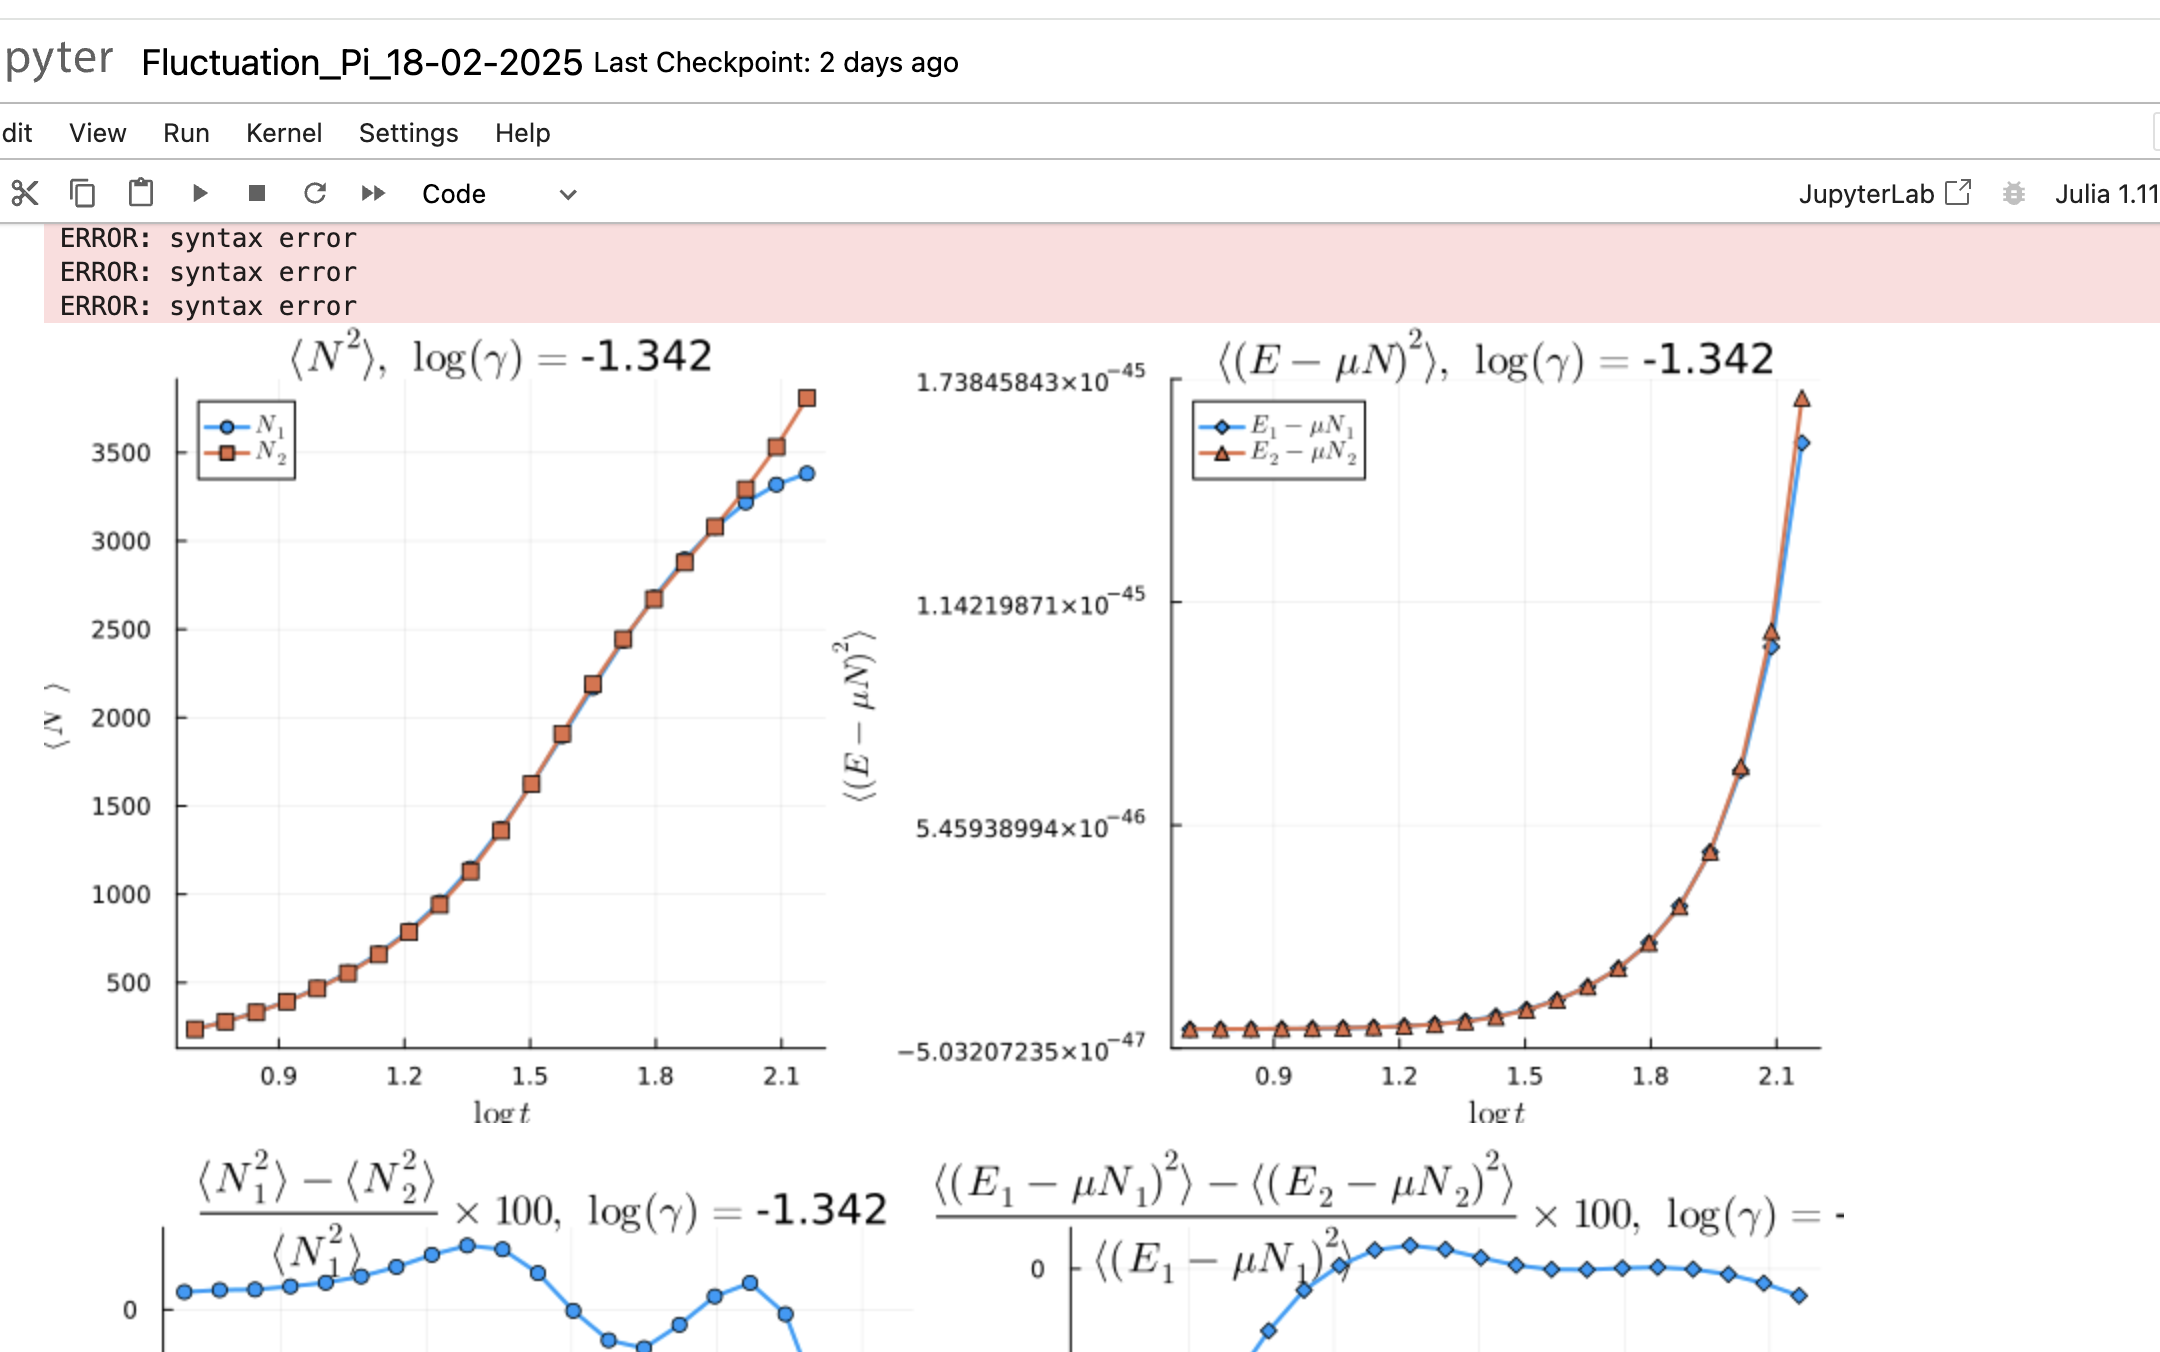
\includegraphics[width=1\textwidth]{Figures/test}

%\begin{aff}
%Donc une a l'ordre un en $\delta \theta (\operator{A}^{(0)})^{-1} %\operator{V}$ 

%\begin{eqnarray*}
%	\langle \delta \Pi ( \theta) \delta \Pi ( \theta') \rangle & = &  ( (\Pi^c_s - \Pi^c)\Pi^c/\Pi^c_s ) ( \theta ) \delta_{\theta, \theta'}/\delta \theta + \mathscr{F}(\theta , \theta' ) ,	
%\end{eqnarray*}

%avec 

%\begin{eqnarray*}
%	\mathscr{F}(\theta , \theta' ) & = & \left [ (\Pi^c_s - \Pi^c )( \theta)  +  (\Pi^c_s - \Pi^c ) ( \theta' )\right ] \frac{\Pi^c}{\Pi^c_s}(\theta)\frac{\Pi^c}{\Pi^c_s}(\theta') \frac{ \Delta( \theta'- \theta )}{ 2 \pi }\\
%	&&  - \left [ (\Pi^c_s - \Pi^c )( \theta)   (\Pi^c_s - \Pi^c ) ( \theta' )\right ] \frac{\Pi^c}{\Pi^c_s}(\theta)\frac{\Pi^c}{\Pi^c_s}(\theta')\int d\theta'' \left (   \frac{ \Pi^c/\Pi^c_s}{\Pi^c_s - \Pi^c} \right )(\theta'') \frac{\Delta(\theta''- \theta)}{2 \pi}\frac{\Delta(\theta''- \theta')}{2 \pi}  	
%\end{eqnarray*}
%\end{aff}



 










%\subsection{États du vide et pseudovacuum}
%%Dans ce chapitre, nous nous intéressons aux fluctuations de la distribution de rapidité \( \delta \rho \) autour d'une distribution de référence \( \rho^c \), qui maximise la contribution à la fonction de partition des états, exprimée comme une fonctionnelle de la distribution \( \rho \) : 

La fonction de partition des états, s'exprime comme une fonctionnelle de la distribution \( \rho \) : 

\begin{eqnarray*}
	\Xi & = & \sum_\rho \exp \left( -\mathcal{A}(\rho) \right).
\end{eqnarray*}  

Dans la section {\em \bf Entropie de Yang-Yang} (\ref{??}), l'action \( \mathcal{A}(\rho) \) s'écrit sous la forme :  

\begin{eqnarray*}
	\mathcal{A}(\rho) & \doteq & - L\mathcal{S}_{YY}(\rho) + L\int f(\theta) \rho (\theta) \, d\theta,		
\end{eqnarray*}  

où \( \mathcal{S}_{YY} \) est la fonctionnelle d'entropie de Yang-Yang, définie dans (\ref{??}), et \( f \) est la fonction paramétrant les charges, introduite dans (\ref{??}).  

Dans cette même section {\em \bf Entropie de Yang-Yang} (\ref{??}), nous avons établi un lien entre \( f \) et distribution de référence \( \rho^c \), qui maximise la contribution à la fonction de partition des états .\\

On veux tester si nos experience est décrit pas un GGE. Pour cela nous nous intéressons aux fluctuations de la distribution de rapidité \( \delta \rho \) autour \( \rho^c \).

%Nous poursuivons à présent avec cette définition de l'action de classe $\mathcal{C}^2$ et admetant une distribution critique $\rho^c$ tel que sa différentielle en ce point critique soit nulle $d\mathcal{A}_{\rho^c} = 0 $ (\ref{??}) de sorte que d'aprés la formule de Taylor-Youg %afin de déterminer les fluctuations autour de \( \Pi^c \). Pour cela, nous réécrivons l'action sous la forme :  

Nous poursuivons à présent avec cette définition de l'action de classe $\mathcal{C}^2$ et admetant une distribution critique $\rho^c$ tel que sa différentielle en ce point critique soit nulle $d\mathcal{A}_{\rho^c} = 0 $ (\ref{??}) de sorte que d'aprés la formule de Taylor-Youg %afin de déterminer les fluctuations autour de \( \Pi^c \). Pour cela, nous réécrivons l'action sous la forme :  

\begin{eqnarray*}  
	\mathcal{A}(\rho^c + \delta \rho) & \underset{ \delta \rho \to 0 }{=} & \mathcal{A}(\rho^c)  + \frac{1}{2} \left. \frac{\delta^2 \mathcal{A}}{\delta \rho^2} \right|_{\rho^c} (\delta \rho) + \mathcal{O}((\delta \rho)^3),  
\end{eqnarray*}  

une expression quadratique pour l'action à l'ordre dominant en \( \delta \Pi \) avec $\left. \frac{\delta^2 \mathcal{A}}{\delta \rho^2} \right|_{\rho^c}$ la forme quadratique définie positive (Fig (\ref{fig.fluctu.A})).

\begin{figure}[H]
	\centering 
	\begin{tikzpicture}
		\begin{scope}[shift={(0,0)}]
			\begin{scope}[transform canvas={scale=0.6}]
				% Définition des couleurs avec les codes HTML
\definecolor{colorOne}{HTML}{443E46}
\definecolor{colorTwo}{HTML}{F6DEB8}
\definecolor{colorThree}{HTML}{908CA4}
\definecolor{colorFour}{HTML}{57659E}
\definecolor{colorFive}{HTML}{C57284}
\definecolor{colorSix}{HTML}{FF5B69}

% Raccourcis pour les couleurs
\def\colorOne{colorOne}
\def\colorTwo{colorTwo}
\def\colorThree{colorThree}
\def\colorFour{colorFour}
\def\colorFive{colorFive}
\def\colorSix{colorSix}

\def\colorslide{blue!50!black}



\begin{scope}
	% Tracer une courbe lisse entre des points
	\draw[shift={(0,0)} ,\colorOne]
		(-1 , 0 ) edge [thick,line width=0.8ex , ->,>=triangle 45  , \colorOne] node [pos = 1 , below ]{\huge$\rho$}( 5  , 0 )
	;
	\draw[shift={(0,0)}, color=\colorOne]
		(0, -1.0 ) edge [thick,line width=0.8ex , ->,>=triangle 45  ]node [pos=0.9,left=0.2cm ]{\huge$\mathcal{A}(\rho)$}( 0  , 5 )
	;
	\draw[]
		(2.5, 0.12 ) edge [thick,line width=0.8ex ,\colorThree ]node [pos=1,below  ]{\huge$\rho^c$} (2.5, -0.12 )	
	;
	
	\draw[]
		(2.5, -0.12 ) edge [thick,line width=0.4ex , dashed, \colorThree ] (2.5, 5.5 )
		(1.5, 1 ) edge [thick,line width=0.4ex , <->,>=triangle 45  , \colorThree ] (3.5, 1 )
		(-0.3,1) edge [thick,line width=0.4ex  , \colorThree ] node [pos=0,left ]{\huge$\mathcal{A}(\rho^c)$} (0.3, 1 )	
	;
    \draw[thick, line width=0.8ex , \colorFour] plot[smooth, tension=0.7] coordinates {
        (1, 5) (1.6 , 3 ) (2.5, 1) (3.5 , 3 )  (4, 5)
    };		
	
\end{scope}

	
			
			\end{scope}
			
			\draw[color = red , scale = 0.5 , draw = none  ] (-2 , -1) rectangle (5, 6) ; 	
		\end{scope}
		
		\begin{scope}[shift={(19,-1)}]
			\begin{scope}[transform canvas={scale=0.6}]
				% Définition des couleurs avec les codes HTML
\definecolor{colorOne}{HTML}{443E46}
\definecolor{colorTwo}{HTML}{F6DEB8}
\definecolor{colorThree}{HTML}{908CA4}
\definecolor{colorFour}{HTML}{57659E}
\definecolor{colorFive}{HTML}{C57284}
\definecolor{colorSix}{HTML}{FF5B69}

% Raccourcis pour les couleurs
\def\colorOne{colorOne}
\def\colorTwo{colorTwo}
\def\colorThree{colorThree}
\def\colorFour{colorFour}
\def\colorFive{colorFive}
\def\colorSix{colorSix}

\def\colorslide{blue!50!black}

\def\Occupation{
	\def\traitx{0.3}
	\def\traity{0.5}
	\draw[shift={(0,0)}]
		(-13.5 , 0 ) edge [thick,line width=0.8ex ]( -3.2  , 0 )
		( -3.2 - \traitx  , 0 - \traity ) edge [thick,line width=0.8ex ]( -3.2 + \traitx  , 0 + \traity  )
		( -2.8 - \traitx  , 0 - \traity ) edge [thick,line width=0.8ex ]( -2.8 + \traitx  , 0 + \traity  )
		(-2.8 , 0 ) edge [thick,line width=0.8ex ](2.8  , 0 )
		( 2.8 - \traitx  , 0 - \traity ) edge [thick,line width=0.8ex ]( 2.8 + \traitx  , 0 + \traity  )
		( 3.2 - \traitx  , 0 - \traity ) edge [thick,line width=0.8ex ]( 3.2 + \traitx  , 0 + \traity  )
		(3.2, 0 ) edge [thick,line width=0.8ex,->,>=triangle 45 , color = black ]node [pos=1.01,below  ]{\huge$\theta$}	( 13  , 0 )
	;
	\draw[shift={(0,0)}, color=\colorOne]
		(-10.5 , -1.5 ) edge [thick,line width=0.8ex , ->,>=triangle 45  ]( -10.5  , 4.5 )
	;
		
	\foreach \r in {1 , ... , 3 } {
%		\draw[
%		decoration={
%		markings,
%    	mark connection node=my node,
%    	mark=at position 0 with{\node [blue,transform shape] (my node) {\large \r};}},
%		color=gray, thick, 
%		line width=0.5ex] decorate { 
%            (-11.0, \r) -- (-10.1, \r )}
%        ;
        \draw[
			color=\colorOne,
			] 
            (-11.0, \r) edge[color=\colorThree , thick,line width=0.5ex] node [pos=-0.5 ]{\large\color{\colorFour} $\frac{\r}{\delta \theta}$ } (-10.3, \r )
        	;
	
	}
	

	
	% Graduation abcsisse 
	% Définitions des listes
% Definitions of the lists
\def\listetuple{-9/\theta_{1}, -8/\theta_{2} , -5/\theta_{3} , -2/\theta_{a-1} , 0/\theta_{a} , 1/\theta_{a+1} , 2/\theta_{a+2} ,  5/\theta_{N-4} , 7/\theta_{N-3},8/\theta_{N-1},9/\theta_{N} }
\def\listetrais{-12 , -11, -10, -9 , -8 , -7 ,  -6 , -5, -4.5,-4, -2 , -1, 0 , 0.5, 1, 2, 4 , 5 ,  6 , 7 , 8 ,8.5, 9 ,  10 , 11, 12 }

% Loop over listetrais
\foreach \r in \listetrais {
    % Initialize found variable to zero
    % Initialize found variable to zero
    %\pgfmathsetmacro\found{0}
    \global\def\found{0}
    \xdef\nomtheta{}
    
    % Check if \r is in listetuple
    \foreach \x/\y in \listetuple { 
        \ifdim \r pt=\x pt % If \r matches any \x in listetuple
            \global\def\found{1} ;
            \xdef\nomtheta{\y} % Set \nomtheta to the corresponding \y
            %\pgfmathsetmacro\found{1} % Set found to 1            
            %\global\pgfmathsetmacro\found{1}
        \fi
    }
    
    %\node [circle, draw, red] (A) at (\r, 2) {\found , $\nomtheta$};
    
    % Draw the line and display \nomtheta if found
    \ifnum\found=1
        \draw[color=\colorOne, thick, line width=0.5ex] 
            (\r, -0.3) -- (\r, 0.3) node[red , pos=-0.5] {\large $\nomtheta$};
         \filldraw[line width=0.5ex, color=\colorSix, outer color=\colorSix, inner color=\colorSix] 
            (\r, 0) circle (4pt);
    \else 
        % Draw without \nomtheta and add a blue circle if not found
        \draw[color=\colorOne, thick, line width=0.5ex] 
            (\r, -0.3) -- (\r, 0.3);
        \filldraw[line width=0.5ex, color=\colorSix, outer color=\colorTwo, inner color=\colorTwo] 
            (\r, 0) circle (4pt); 
    \fi
}

\def\listetrais{-9.5/\theta_{i-1}/2/3, -6.5/\theta_{i}/1/4  ,   -1.5/\theta_{j}/2/4 , 1.5/\theta_{j+1}/-1/3 , 3.5/\theta_{\ell-1}/1/3 , 6.5/\theta_{\ell}/3/4 , 9.5/\theta(\theta_{\ell+1})/-1/3 };



\foreach \r/\nomx/\y/\ys in \listetrais {
	\draw[
		decoration={
		markings,
    	mark connection node=my node,
    	mark=at position .5 with{\node [blue,transform shape] (my node) {\large \color{\colorFour} $\nomx$};}},
		color=\colorThree , thick, 
		line width=0.5ex] decorate { 
            (\r, 0.12) -- (\r, -1.2)}
        ;
     
     \ifdim \y pt > -1 pt 
     	\draw[
			decoration={
			markings,
    		mark connection node=my node,
    		mark=at position .5 with{\node [blue,transform shape] (my node) {\large \color{\colorFour} $\Pi(\nomx) $};}},
			color=\colorThree, thick, 
			line width=0.5ex] decorate { 
            (\r, \y) -- (\r +3, \y)}
        ;
        \draw[
			decoration={
			markings,
    		mark connection node=my node,
    		mark=at position .5 with{\node [blue,transform shape] (my node) {\large \color{\colorFive} $\Pi_s(\nomx) $};}},
			color=\colorFive, thick, 
			line width=0.5ex] decorate { 
            (\r, \ys) -- (\r +3, \ys)}
        ;
     \fi 
     \ifdim \r pt= -1.5 pt
     	\draw[
     		decoration={
			markings,
    		mark connection node=my node,
    		mark=at position .5 with{\node [blue,transform shape] (my node) {\large \color{\colorFour}  $\delta \theta $};},
    		%mark=at position 0.1  with {\arrow[blue, line width=0.5ex]{<}},
    		%mark=at position 1  with {\arrow[blue, line width=0.5ex]{>}}
    		},
        	color=\colorThree,
        	thick,
        	line width=0.5ex,
        	%arrows={Computer Modern Rightarrow[line cap=round]-Computer Modern Rightarrow[line cap=round]}
   			](\r, -1.2) edge[arrows={Computer Modern Rightarrow[line cap=round]-}] (\r + 0.4, -1.2)decorate {
    		(\r, -1.2) -- (\r + 3, -1.2)}(\r + 2, -1.2) edge[arrows={-Computer Modern Rightarrow[line cap=round]}] (\r + 3, -1.2)
    		;
    \fi
			
	
}


			
}


\begin{scope}
	%\draw[help lines , width=1.5ex] (-8,-3) grid (8,3);\draw[help lines ,width=0.5ex , opacity = 0.5] (-3,-3) grid[step=0.1] (3,3));
	
	%\draw[help lines] 
	%	(-3,-3) edge[width=1.5ex] grid (3,3)	
	%	(-3,-3) edge[width=0.5ex , opacity = 0.5] grid (3,3)	
	%;
	\begin{scope}[shift={(0,1)},rotate=0,opacity=1,color=black]
		\Occupation	
		
		%\node[anchor=east, font=\bfseries] at (-11, 0) {\color{red}\large (T = 0 )} ;	
	\end{scope}
	
	
	
	
	\begin{scope}[shift={(-10.5,7)},rotate=0,opacity=1,color=black]
	
	\begin{scope}[shift={(-0,0)},rotate=0,opacity=1,color=black]
	
		\draw[shift={(0,0)} ,line width=1ex,rounded corners = 1ex,color=\colorOne , opacity =1 ,fill=\colorOne!00 , pattern={north east lines} , pattern color=\colorOne!00 ]
			(0 , -1 ) rectangle (5,1)
		;
		

		\begin{scope}[shift={(0.5,0.5)}]
			\draw[color=\colorOne, thick, line width=0.5ex] 
            (0, -0.3) -- (0, 0.3) ;
            \filldraw[line width=0.5ex, color=\colorSix, outer color=\colorSix, inner color=\colorSix] 
            (0, 0) circle (4pt);
            
            \node[anchor=west, font=\bfseries] at (0.2, 0) {\color{\colorSix}\large : quasi-particule};
		\end{scope}
		
		\begin{scope}[shift={(0.5,-0.5)}]
			\draw[color=\colorOne, thick, line width=0.5ex] 
            (0, -0.3) -- (0, 0.3) ;
            \filldraw[line width=0.5ex, color=\colorSix, outer color=\colorTwo, inner color=\colorTwo] 
            (0, 0) circle (4pt);
            
            \node[anchor=west, font=\bfseries] at (0.2, 0) {\color{\colorSix}\large : hole};
		\end{scope}

	\end{scope}
	
	\begin{scope}[shift={(6,0)},rotate=0,opacity=1,color=black]	
		
		\draw[shift={(0,0)} ,line width=1ex,rounded corners = 1ex,color=\colorOne , opacity =1 ,fill=\colorOne!00 , pattern={north east lines} , pattern color=\colorOne!00 ]
			(0 , -1 ) rectangle (7.5,1)
		;
		
		\node[anchor=west] at (0.5, 0.5) {\color{\colorFour}\large $\Pi$ };\node[anchor=west, font=\bfseries] at (1, 0.5) {\color{\colorFour}\large : quasi-particule distribution};
		
		\node[anchor=west] at (0.5, -0.5) {\color{\colorFour}\large $\Pi_h$ };\node[anchor=west, font=\bfseries] at (1, -0.5) {\color{\colorFour}\large  : hole distribution};
		
	\end{scope}
	
	\begin{scope}[shift={(14.5,0)},rotate=0,opacity=1,color=black]	
		
		\draw[shift={(0,0)} ,line width=1ex,rounded corners = 1ex,color=\colorOne , opacity =1 ,fill=\colorOne!00 , pattern={north east lines} , pattern color=\colorOne!00 ]
			(0 , -0.5 ) rectangle (7.0,0.5)
		;
		
		\node[anchor=west] at (0.2, 0) {\color{\colorFour}\large ${\color{\colorFive}\Pi_s} = \Pi + \Pi_h $ } node[anchor=west , font=\bfseries] at (3.1 , 0 )  {\color{\colorFour}\large {\color{\colorFive} : density of states}};
		
	\end{scope}
	
	
	\end{scope}


		
	
\end{scope}

	
			
			\end{scope}
			\begin{scope}[scale=1]
				\draw[color = red , scale = 1 , draw = none  ] (-1 , -1) rectangle (5, 5) ; 
			\end{scope}	
		\end{scope}

		
				
			
	\end{tikzpicture}	
	\captionsetup{skip=10pt} % Ajoute de l’espace après la légende
	\label{fig.fluctu.A}
\end{figure}


On discrétise l'axe des rapidités en  petite cellule de rapidité $[\theta, \theta+\delta\theta]$, qui contient $L\rho(\theta) \delta \theta$ rapidités. 
	



Avec ces petites tranches, la forme quadratique s’écrit :

\begin{eqnarray*}
    \left. \frac{\delta^2 \mathcal{A}}{{\delta \rho}^2} \right|_{\rho^c}(\delta \rho ) &=&  \sum_{a,b \mid \text{tranche}}  
    \delta \rho(\theta_a)  \frac{\partial^2 \mathcal{A}}{\partial \delta \rho(\theta_a) \partial \delta \rho(\theta_b) } (\rho^c)  \delta \rho(\theta_b).
\end{eqnarray*}
Les fluctuations s’écrivent donc :

\begin{eqnarray*}
    \langle \delta \rho ( \theta) \delta \rho ( \theta') \rangle &=&  
    \frac{ \int d\delta \rho \, \delta \rho(\theta) \delta \rho ( \theta') 
    \exp \left( - \frac{1}{2} \sum_{a,b \mid \text{tranche}}  
    \delta \rho(\theta_a) \frac{\partial^2 \mathcal{A}}{\partial \delta \rho(\theta_a) \partial \delta \rho(\theta_b) } (\rho^c)  \delta \rho(\theta_b) \right) }
    { \int d\delta \Pi  
    \exp \left( - \frac{1}{2} \sum_{a,b \mid \text{tranche}}  
    \delta \rho(\theta_a) \frac{\partial^2 \mathcal{A}}{\partial \delta \rho(\theta_a) \partial \delta \rho(\theta_b) } (\rho^c)  \delta \rho(\theta_b) \right) } \\
    &=& \left( \mathbf{A}^{-1} \right)_{\theta , \theta'}
\end{eqnarray*}


\begin{aff}

\begin{eqnarray*}
	\langle \delta \rho ( \theta) \delta \rho ( \theta') \rangle &=& 	\left( \mathbf{A}^{-1} \right)_{\theta , \theta'}
\end{eqnarray*}

	
avec la  {\em matrice hessienne} $\mathbf{A}_{\theta , \theta'} \equiv \frac{\partial^2 \mathcal{A}}{\partial \delta \rho(\theta) \partial \delta \rho(\theta') }(\rho^c)$, au point critique/ qui maximise la probabilité  $\rho^c=\rho^c_s \nu^c $, s'écrit

\begin{eqnarray*}
	\operator{A} & = & \operator{A}^{(0)} + \delta \theta \operator{V}
\end{eqnarray*}

avec 

\begin{eqnarray*}
	A^{(0)}_{\theta , \theta'}  & = &  L\delta \theta \left ( \frac{ 1}{\rho^c_s ( 1  - \nu^c ) \nu^c } \right )(\theta)    \delta({\theta - \theta '})	,\\
	V_{\theta , \theta'}  &= & L \delta \theta \left \{ - \left [ \left ( \frac{1}{\rho^c_s( 1 - \nu^c) } \right ) ( \theta)  +  \left ( \frac{1}{\rho^c_s( 1 - \nu^c) } \right ) ( \theta' )\right ] \frac{ \Delta( \theta'- \theta )}{ 2 \pi } + \int d\theta''  \left ( \frac{\nu^c}{\rho^c_s( 1 - \nu^c) } \right )(\theta'') \frac{\Delta(\theta''- \theta)}{2 \pi}\frac{\Delta(\theta''- \theta')}{2 \pi}   \right \} 	
\end{eqnarray*}

\end{aff}

\subsection{Testes}

\begin{eqnarray*}
	\Delta_{\operator{\mathcal{N}}}^2  & = &  \frac{1}{\beta} \left . \frac{\partial \langle \operator{\mathcal{N}} \rangle}{\partial \mu} \right )_T \\
	\Delta_{\operator{\mathcal{E}}-\mu \operator{\mathcal{N}}}^2  & = &  - \left . \frac{\partial \langle \operator{\mathcal{E}}-\mu \operator{\mathcal{N}} \rangle}{\partial \beta} \right )_\mu 
\end{eqnarray*}

et 

\begin{eqnarray*}
	\Delta_{\operator{\mathcal{N}}}^2  &= & L^2 \int d\theta_a \int d \theta_b \, \langle \delta \rho(\theta_a) \delta \rho(\theta_b) \rangle \\
	\Delta_{\operator{\mathcal{E}}-\mu \operator{\mathcal{N}}}^2  & = & L^2 \int d\theta_a \int d \theta_b \, \left ( - \mu + \frac{1}2 m \theta_a^2  \right  )\left ( - \mu + \frac{1}2 m \theta_b^2  \right  )  \langle \delta \rho(\theta_a) \delta \rho(\theta_b) \rangle
\end{eqnarray*}

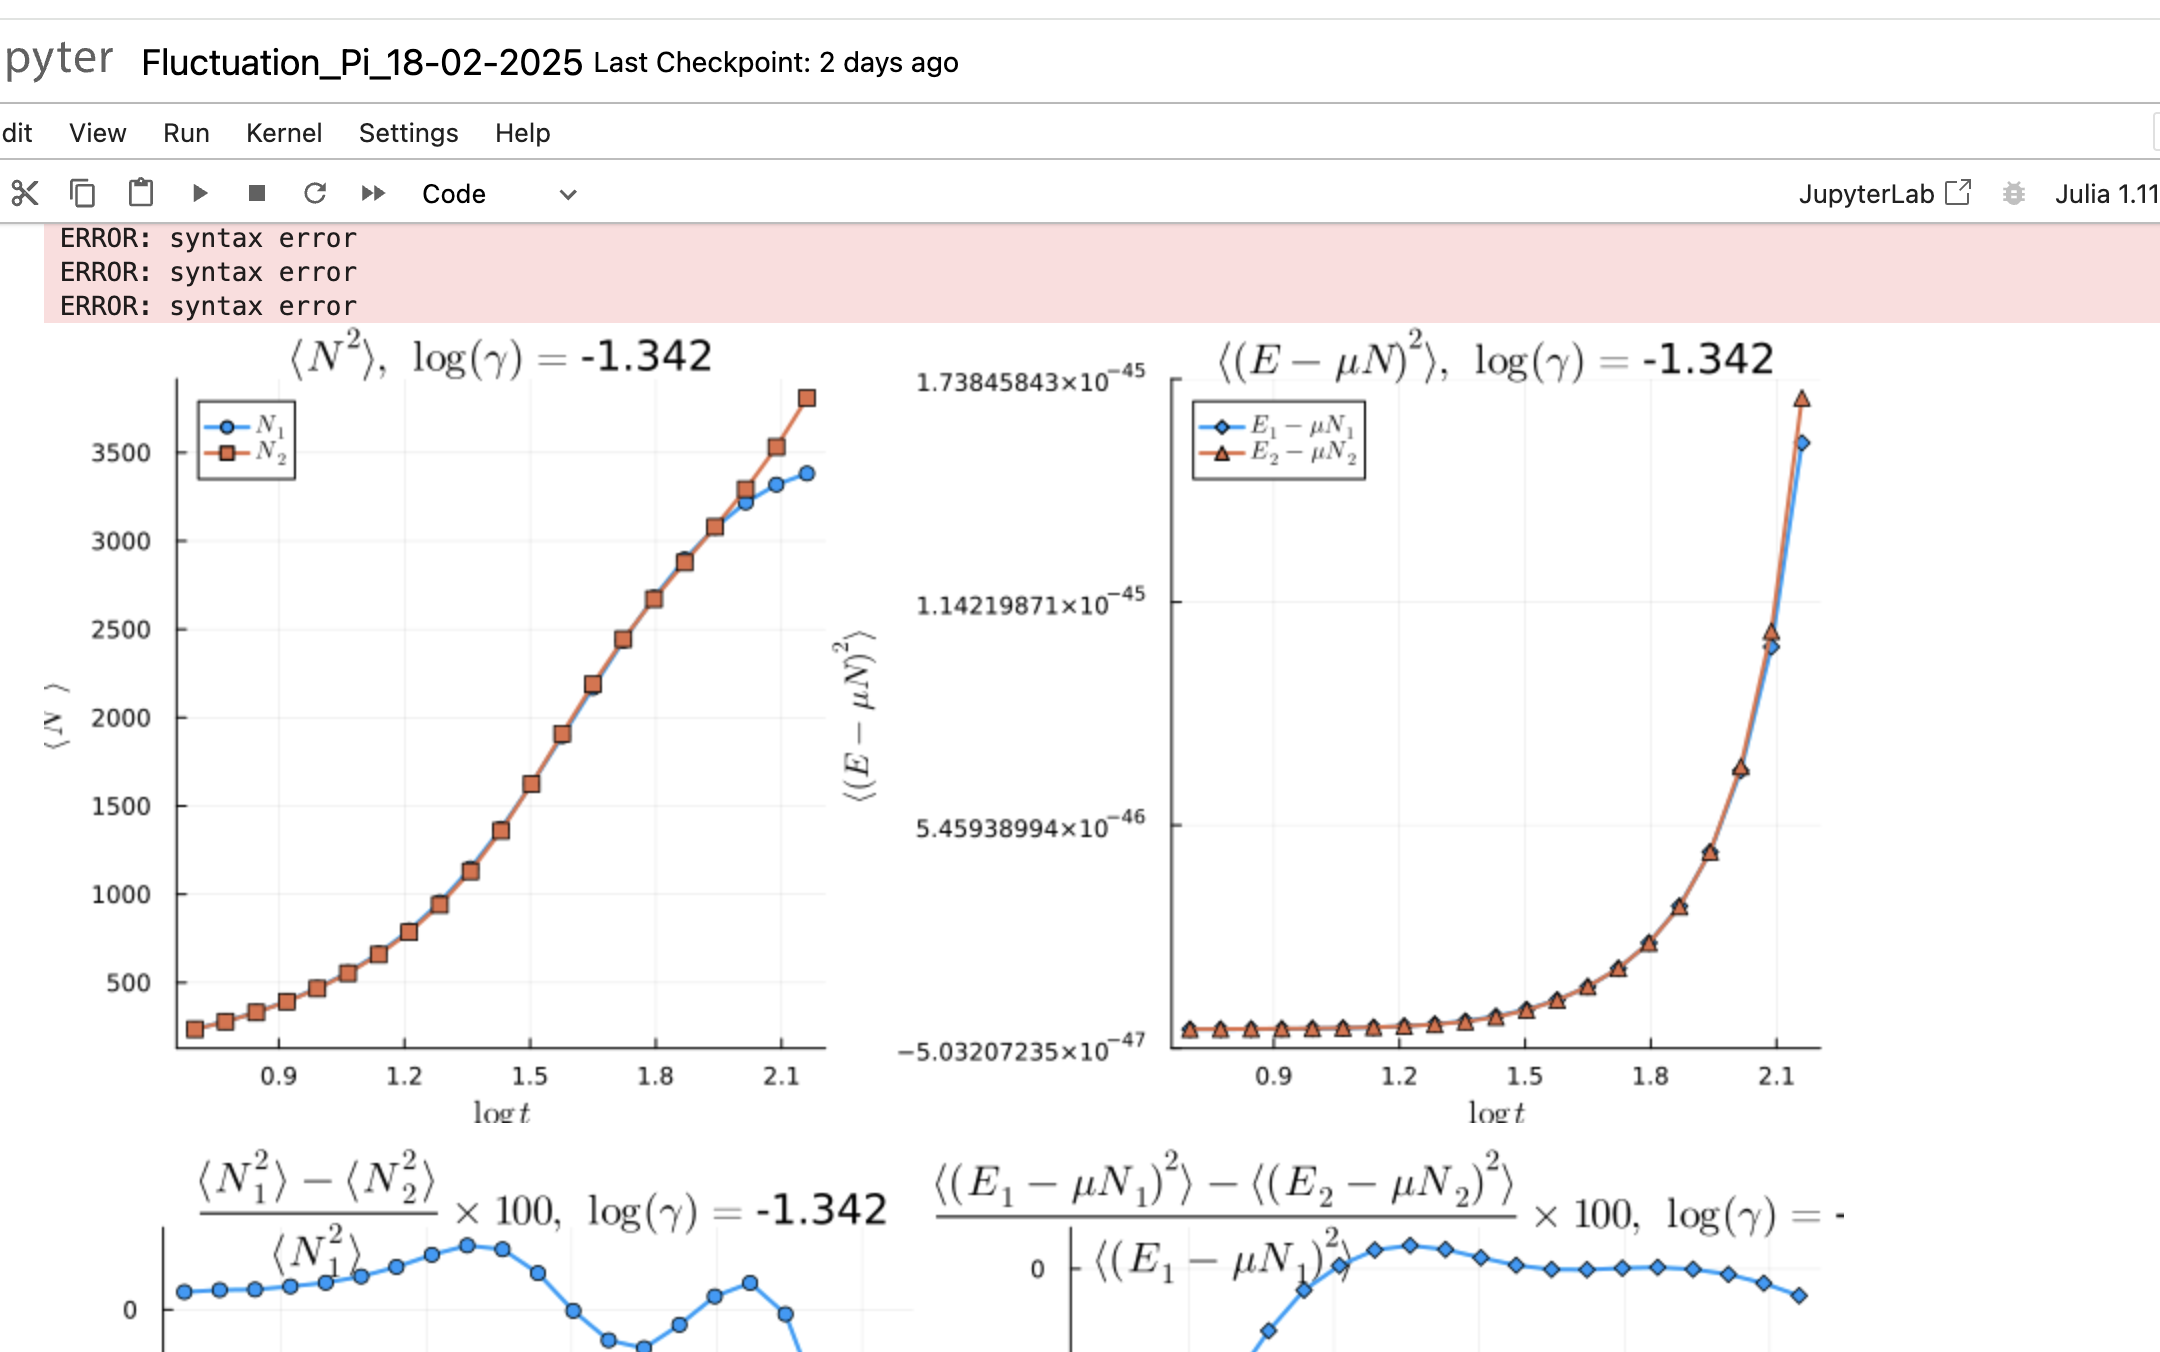
\includegraphics[width=1\textwidth]{Figures/test}

%\begin{aff}
%Donc une a l'ordre un en $\delta \theta (\operator{A}^{(0)})^{-1} %\operator{V}$ 

%\begin{eqnarray*}
%	\langle \delta \Pi ( \theta) \delta \Pi ( \theta') \rangle & = &  ( (\Pi^c_s - \Pi^c)\Pi^c/\Pi^c_s ) ( \theta ) \delta_{\theta, \theta'}/\delta \theta + \mathscr{F}(\theta , \theta' ) ,	
%\end{eqnarray*}

%avec 

%\begin{eqnarray*}
%	\mathscr{F}(\theta , \theta' ) & = & \left [ (\Pi^c_s - \Pi^c )( \theta)  +  (\Pi^c_s - \Pi^c ) ( \theta' )\right ] \frac{\Pi^c}{\Pi^c_s}(\theta)\frac{\Pi^c}{\Pi^c_s}(\theta') \frac{ \Delta( \theta'- \theta )}{ 2 \pi }\\
%	&&  - \left [ (\Pi^c_s - \Pi^c )( \theta)   (\Pi^c_s - \Pi^c ) ( \theta' )\right ] \frac{\Pi^c}{\Pi^c_s}(\theta)\frac{\Pi^c}{\Pi^c_s}(\theta')\int d\theta'' \left (   \frac{ \Pi^c/\Pi^c_s}{\Pi^c_s - \Pi^c} \right )(\theta'') \frac{\Delta(\theta''- \theta)}{2 \pi}\frac{\Delta(\theta''- \theta')}{2 \pi}  	
%\end{eqnarray*}
%\end{aff}



 










%\subsection{Opérateurs conservés (intégrales du mouvement)}
%%Dans ce chapitre, nous nous intéressons aux fluctuations de la distribution de rapidité \( \delta \rho \) autour d'une distribution de référence \( \rho^c \), qui maximise la contribution à la fonction de partition des états, exprimée comme une fonctionnelle de la distribution \( \rho \) : 

La fonction de partition des états, s'exprime comme une fonctionnelle de la distribution \( \rho \) : 

\begin{eqnarray*}
	\Xi & = & \sum_\rho \exp \left( -\mathcal{A}(\rho) \right).
\end{eqnarray*}  

Dans la section {\em \bf Entropie de Yang-Yang} (\ref{??}), l'action \( \mathcal{A}(\rho) \) s'écrit sous la forme :  

\begin{eqnarray*}
	\mathcal{A}(\rho) & \doteq & - L\mathcal{S}_{YY}(\rho) + L\int f(\theta) \rho (\theta) \, d\theta,		
\end{eqnarray*}  

où \( \mathcal{S}_{YY} \) est la fonctionnelle d'entropie de Yang-Yang, définie dans (\ref{??}), et \( f \) est la fonction paramétrant les charges, introduite dans (\ref{??}).  

Dans cette même section {\em \bf Entropie de Yang-Yang} (\ref{??}), nous avons établi un lien entre \( f \) et distribution de référence \( \rho^c \), qui maximise la contribution à la fonction de partition des états .\\

On veux tester si nos experience est décrit pas un GGE. Pour cela nous nous intéressons aux fluctuations de la distribution de rapidité \( \delta \rho \) autour \( \rho^c \).

%Nous poursuivons à présent avec cette définition de l'action de classe $\mathcal{C}^2$ et admetant une distribution critique $\rho^c$ tel que sa différentielle en ce point critique soit nulle $d\mathcal{A}_{\rho^c} = 0 $ (\ref{??}) de sorte que d'aprés la formule de Taylor-Youg %afin de déterminer les fluctuations autour de \( \Pi^c \). Pour cela, nous réécrivons l'action sous la forme :  

Nous poursuivons à présent avec cette définition de l'action de classe $\mathcal{C}^2$ et admetant une distribution critique $\rho^c$ tel que sa différentielle en ce point critique soit nulle $d\mathcal{A}_{\rho^c} = 0 $ (\ref{??}) de sorte que d'aprés la formule de Taylor-Youg %afin de déterminer les fluctuations autour de \( \Pi^c \). Pour cela, nous réécrivons l'action sous la forme :  

\begin{eqnarray*}  
	\mathcal{A}(\rho^c + \delta \rho) & \underset{ \delta \rho \to 0 }{=} & \mathcal{A}(\rho^c)  + \frac{1}{2} \left. \frac{\delta^2 \mathcal{A}}{\delta \rho^2} \right|_{\rho^c} (\delta \rho) + \mathcal{O}((\delta \rho)^3),  
\end{eqnarray*}  

une expression quadratique pour l'action à l'ordre dominant en \( \delta \Pi \) avec $\left. \frac{\delta^2 \mathcal{A}}{\delta \rho^2} \right|_{\rho^c}$ la forme quadratique définie positive (Fig (\ref{fig.fluctu.A})).

\begin{figure}[H]
	\centering 
	\begin{tikzpicture}
		\begin{scope}[shift={(0,0)}]
			\begin{scope}[transform canvas={scale=0.6}]
				% Définition des couleurs avec les codes HTML
\definecolor{colorOne}{HTML}{443E46}
\definecolor{colorTwo}{HTML}{F6DEB8}
\definecolor{colorThree}{HTML}{908CA4}
\definecolor{colorFour}{HTML}{57659E}
\definecolor{colorFive}{HTML}{C57284}
\definecolor{colorSix}{HTML}{FF5B69}

% Raccourcis pour les couleurs
\def\colorOne{colorOne}
\def\colorTwo{colorTwo}
\def\colorThree{colorThree}
\def\colorFour{colorFour}
\def\colorFive{colorFive}
\def\colorSix{colorSix}

\def\colorslide{blue!50!black}



\begin{scope}
	% Tracer une courbe lisse entre des points
	\draw[shift={(0,0)} ,\colorOne]
		(-1 , 0 ) edge [thick,line width=0.8ex , ->,>=triangle 45  , \colorOne] node [pos = 1 , below ]{\huge$\rho$}( 5  , 0 )
	;
	\draw[shift={(0,0)}, color=\colorOne]
		(0, -1.0 ) edge [thick,line width=0.8ex , ->,>=triangle 45  ]node [pos=0.9,left=0.2cm ]{\huge$\mathcal{A}(\rho)$}( 0  , 5 )
	;
	\draw[]
		(2.5, 0.12 ) edge [thick,line width=0.8ex ,\colorThree ]node [pos=1,below  ]{\huge$\rho^c$} (2.5, -0.12 )	
	;
	
	\draw[]
		(2.5, -0.12 ) edge [thick,line width=0.4ex , dashed, \colorThree ] (2.5, 5.5 )
		(1.5, 1 ) edge [thick,line width=0.4ex , <->,>=triangle 45  , \colorThree ] (3.5, 1 )
		(-0.3,1) edge [thick,line width=0.4ex  , \colorThree ] node [pos=0,left ]{\huge$\mathcal{A}(\rho^c)$} (0.3, 1 )	
	;
    \draw[thick, line width=0.8ex , \colorFour] plot[smooth, tension=0.7] coordinates {
        (1, 5) (1.6 , 3 ) (2.5, 1) (3.5 , 3 )  (4, 5)
    };		
	
\end{scope}

	
			
			\end{scope}
			
			\draw[color = red , scale = 0.5 , draw = none  ] (-2 , -1) rectangle (5, 6) ; 	
		\end{scope}
		
		\begin{scope}[shift={(19,-1)}]
			\begin{scope}[transform canvas={scale=0.6}]
				% Définition des couleurs avec les codes HTML
\definecolor{colorOne}{HTML}{443E46}
\definecolor{colorTwo}{HTML}{F6DEB8}
\definecolor{colorThree}{HTML}{908CA4}
\definecolor{colorFour}{HTML}{57659E}
\definecolor{colorFive}{HTML}{C57284}
\definecolor{colorSix}{HTML}{FF5B69}

% Raccourcis pour les couleurs
\def\colorOne{colorOne}
\def\colorTwo{colorTwo}
\def\colorThree{colorThree}
\def\colorFour{colorFour}
\def\colorFive{colorFive}
\def\colorSix{colorSix}

\def\colorslide{blue!50!black}

\def\Occupation{
	\def\traitx{0.3}
	\def\traity{0.5}
	\draw[shift={(0,0)}]
		(-13.5 , 0 ) edge [thick,line width=0.8ex ]( -3.2  , 0 )
		( -3.2 - \traitx  , 0 - \traity ) edge [thick,line width=0.8ex ]( -3.2 + \traitx  , 0 + \traity  )
		( -2.8 - \traitx  , 0 - \traity ) edge [thick,line width=0.8ex ]( -2.8 + \traitx  , 0 + \traity  )
		(-2.8 , 0 ) edge [thick,line width=0.8ex ](2.8  , 0 )
		( 2.8 - \traitx  , 0 - \traity ) edge [thick,line width=0.8ex ]( 2.8 + \traitx  , 0 + \traity  )
		( 3.2 - \traitx  , 0 - \traity ) edge [thick,line width=0.8ex ]( 3.2 + \traitx  , 0 + \traity  )
		(3.2, 0 ) edge [thick,line width=0.8ex,->,>=triangle 45 , color = black ]node [pos=1.01,below  ]{\huge$\theta$}	( 13  , 0 )
	;
	\draw[shift={(0,0)}, color=\colorOne]
		(-10.5 , -1.5 ) edge [thick,line width=0.8ex , ->,>=triangle 45  ]( -10.5  , 4.5 )
	;
		
	\foreach \r in {1 , ... , 3 } {
%		\draw[
%		decoration={
%		markings,
%    	mark connection node=my node,
%    	mark=at position 0 with{\node [blue,transform shape] (my node) {\large \r};}},
%		color=gray, thick, 
%		line width=0.5ex] decorate { 
%            (-11.0, \r) -- (-10.1, \r )}
%        ;
        \draw[
			color=\colorOne,
			] 
            (-11.0, \r) edge[color=\colorThree , thick,line width=0.5ex] node [pos=-0.5 ]{\large\color{\colorFour} $\frac{\r}{\delta \theta}$ } (-10.3, \r )
        	;
	
	}
	

	
	% Graduation abcsisse 
	% Définitions des listes
% Definitions of the lists
\def\listetuple{-9/\theta_{1}, -8/\theta_{2} , -5/\theta_{3} , -2/\theta_{a-1} , 0/\theta_{a} , 1/\theta_{a+1} , 2/\theta_{a+2} ,  5/\theta_{N-4} , 7/\theta_{N-3},8/\theta_{N-1},9/\theta_{N} }
\def\listetrais{-12 , -11, -10, -9 , -8 , -7 ,  -6 , -5, -4.5,-4, -2 , -1, 0 , 0.5, 1, 2, 4 , 5 ,  6 , 7 , 8 ,8.5, 9 ,  10 , 11, 12 }

% Loop over listetrais
\foreach \r in \listetrais {
    % Initialize found variable to zero
    % Initialize found variable to zero
    %\pgfmathsetmacro\found{0}
    \global\def\found{0}
    \xdef\nomtheta{}
    
    % Check if \r is in listetuple
    \foreach \x/\y in \listetuple { 
        \ifdim \r pt=\x pt % If \r matches any \x in listetuple
            \global\def\found{1} ;
            \xdef\nomtheta{\y} % Set \nomtheta to the corresponding \y
            %\pgfmathsetmacro\found{1} % Set found to 1            
            %\global\pgfmathsetmacro\found{1}
        \fi
    }
    
    %\node [circle, draw, red] (A) at (\r, 2) {\found , $\nomtheta$};
    
    % Draw the line and display \nomtheta if found
    \ifnum\found=1
        \draw[color=\colorOne, thick, line width=0.5ex] 
            (\r, -0.3) -- (\r, 0.3) node[red , pos=-0.5] {\large $\nomtheta$};
         \filldraw[line width=0.5ex, color=\colorSix, outer color=\colorSix, inner color=\colorSix] 
            (\r, 0) circle (4pt);
    \else 
        % Draw without \nomtheta and add a blue circle if not found
        \draw[color=\colorOne, thick, line width=0.5ex] 
            (\r, -0.3) -- (\r, 0.3);
        \filldraw[line width=0.5ex, color=\colorSix, outer color=\colorTwo, inner color=\colorTwo] 
            (\r, 0) circle (4pt); 
    \fi
}

\def\listetrais{-9.5/\theta_{i-1}/2/3, -6.5/\theta_{i}/1/4  ,   -1.5/\theta_{j}/2/4 , 1.5/\theta_{j+1}/-1/3 , 3.5/\theta_{\ell-1}/1/3 , 6.5/\theta_{\ell}/3/4 , 9.5/\theta(\theta_{\ell+1})/-1/3 };



\foreach \r/\nomx/\y/\ys in \listetrais {
	\draw[
		decoration={
		markings,
    	mark connection node=my node,
    	mark=at position .5 with{\node [blue,transform shape] (my node) {\large \color{\colorFour} $\nomx$};}},
		color=\colorThree , thick, 
		line width=0.5ex] decorate { 
            (\r, 0.12) -- (\r, -1.2)}
        ;
     
     \ifdim \y pt > -1 pt 
     	\draw[
			decoration={
			markings,
    		mark connection node=my node,
    		mark=at position .5 with{\node [blue,transform shape] (my node) {\large \color{\colorFour} $\Pi(\nomx) $};}},
			color=\colorThree, thick, 
			line width=0.5ex] decorate { 
            (\r, \y) -- (\r +3, \y)}
        ;
        \draw[
			decoration={
			markings,
    		mark connection node=my node,
    		mark=at position .5 with{\node [blue,transform shape] (my node) {\large \color{\colorFive} $\Pi_s(\nomx) $};}},
			color=\colorFive, thick, 
			line width=0.5ex] decorate { 
            (\r, \ys) -- (\r +3, \ys)}
        ;
     \fi 
     \ifdim \r pt= -1.5 pt
     	\draw[
     		decoration={
			markings,
    		mark connection node=my node,
    		mark=at position .5 with{\node [blue,transform shape] (my node) {\large \color{\colorFour}  $\delta \theta $};},
    		%mark=at position 0.1  with {\arrow[blue, line width=0.5ex]{<}},
    		%mark=at position 1  with {\arrow[blue, line width=0.5ex]{>}}
    		},
        	color=\colorThree,
        	thick,
        	line width=0.5ex,
        	%arrows={Computer Modern Rightarrow[line cap=round]-Computer Modern Rightarrow[line cap=round]}
   			](\r, -1.2) edge[arrows={Computer Modern Rightarrow[line cap=round]-}] (\r + 0.4, -1.2)decorate {
    		(\r, -1.2) -- (\r + 3, -1.2)}(\r + 2, -1.2) edge[arrows={-Computer Modern Rightarrow[line cap=round]}] (\r + 3, -1.2)
    		;
    \fi
			
	
}


			
}


\begin{scope}
	%\draw[help lines , width=1.5ex] (-8,-3) grid (8,3);\draw[help lines ,width=0.5ex , opacity = 0.5] (-3,-3) grid[step=0.1] (3,3));
	
	%\draw[help lines] 
	%	(-3,-3) edge[width=1.5ex] grid (3,3)	
	%	(-3,-3) edge[width=0.5ex , opacity = 0.5] grid (3,3)	
	%;
	\begin{scope}[shift={(0,1)},rotate=0,opacity=1,color=black]
		\Occupation	
		
		%\node[anchor=east, font=\bfseries] at (-11, 0) {\color{red}\large (T = 0 )} ;	
	\end{scope}
	
	
	
	
	\begin{scope}[shift={(-10.5,7)},rotate=0,opacity=1,color=black]
	
	\begin{scope}[shift={(-0,0)},rotate=0,opacity=1,color=black]
	
		\draw[shift={(0,0)} ,line width=1ex,rounded corners = 1ex,color=\colorOne , opacity =1 ,fill=\colorOne!00 , pattern={north east lines} , pattern color=\colorOne!00 ]
			(0 , -1 ) rectangle (5,1)
		;
		

		\begin{scope}[shift={(0.5,0.5)}]
			\draw[color=\colorOne, thick, line width=0.5ex] 
            (0, -0.3) -- (0, 0.3) ;
            \filldraw[line width=0.5ex, color=\colorSix, outer color=\colorSix, inner color=\colorSix] 
            (0, 0) circle (4pt);
            
            \node[anchor=west, font=\bfseries] at (0.2, 0) {\color{\colorSix}\large : quasi-particule};
		\end{scope}
		
		\begin{scope}[shift={(0.5,-0.5)}]
			\draw[color=\colorOne, thick, line width=0.5ex] 
            (0, -0.3) -- (0, 0.3) ;
            \filldraw[line width=0.5ex, color=\colorSix, outer color=\colorTwo, inner color=\colorTwo] 
            (0, 0) circle (4pt);
            
            \node[anchor=west, font=\bfseries] at (0.2, 0) {\color{\colorSix}\large : hole};
		\end{scope}

	\end{scope}
	
	\begin{scope}[shift={(6,0)},rotate=0,opacity=1,color=black]	
		
		\draw[shift={(0,0)} ,line width=1ex,rounded corners = 1ex,color=\colorOne , opacity =1 ,fill=\colorOne!00 , pattern={north east lines} , pattern color=\colorOne!00 ]
			(0 , -1 ) rectangle (7.5,1)
		;
		
		\node[anchor=west] at (0.5, 0.5) {\color{\colorFour}\large $\Pi$ };\node[anchor=west, font=\bfseries] at (1, 0.5) {\color{\colorFour}\large : quasi-particule distribution};
		
		\node[anchor=west] at (0.5, -0.5) {\color{\colorFour}\large $\Pi_h$ };\node[anchor=west, font=\bfseries] at (1, -0.5) {\color{\colorFour}\large  : hole distribution};
		
	\end{scope}
	
	\begin{scope}[shift={(14.5,0)},rotate=0,opacity=1,color=black]	
		
		\draw[shift={(0,0)} ,line width=1ex,rounded corners = 1ex,color=\colorOne , opacity =1 ,fill=\colorOne!00 , pattern={north east lines} , pattern color=\colorOne!00 ]
			(0 , -0.5 ) rectangle (7.0,0.5)
		;
		
		\node[anchor=west] at (0.2, 0) {\color{\colorFour}\large ${\color{\colorFive}\Pi_s} = \Pi + \Pi_h $ } node[anchor=west , font=\bfseries] at (3.1 , 0 )  {\color{\colorFour}\large {\color{\colorFive} : density of states}};
		
	\end{scope}
	
	
	\end{scope}


		
	
\end{scope}

	
			
			\end{scope}
			\begin{scope}[scale=1]
				\draw[color = red , scale = 1 , draw = none  ] (-1 , -1) rectangle (5, 5) ; 
			\end{scope}	
		\end{scope}

		
				
			
	\end{tikzpicture}	
	\captionsetup{skip=10pt} % Ajoute de l’espace après la légende
	\label{fig.fluctu.A}
\end{figure}


On discrétise l'axe des rapidités en  petite cellule de rapidité $[\theta, \theta+\delta\theta]$, qui contient $L\rho(\theta) \delta \theta$ rapidités. 
	



Avec ces petites tranches, la forme quadratique s’écrit :

\begin{eqnarray*}
    \left. \frac{\delta^2 \mathcal{A}}{{\delta \rho}^2} \right|_{\rho^c}(\delta \rho ) &=&  \sum_{a,b \mid \text{tranche}}  
    \delta \rho(\theta_a)  \frac{\partial^2 \mathcal{A}}{\partial \delta \rho(\theta_a) \partial \delta \rho(\theta_b) } (\rho^c)  \delta \rho(\theta_b).
\end{eqnarray*}
Les fluctuations s’écrivent donc :

\begin{eqnarray*}
    \langle \delta \rho ( \theta) \delta \rho ( \theta') \rangle &=&  
    \frac{ \int d\delta \rho \, \delta \rho(\theta) \delta \rho ( \theta') 
    \exp \left( - \frac{1}{2} \sum_{a,b \mid \text{tranche}}  
    \delta \rho(\theta_a) \frac{\partial^2 \mathcal{A}}{\partial \delta \rho(\theta_a) \partial \delta \rho(\theta_b) } (\rho^c)  \delta \rho(\theta_b) \right) }
    { \int d\delta \Pi  
    \exp \left( - \frac{1}{2} \sum_{a,b \mid \text{tranche}}  
    \delta \rho(\theta_a) \frac{\partial^2 \mathcal{A}}{\partial \delta \rho(\theta_a) \partial \delta \rho(\theta_b) } (\rho^c)  \delta \rho(\theta_b) \right) } \\
    &=& \left( \mathbf{A}^{-1} \right)_{\theta , \theta'}
\end{eqnarray*}


\begin{aff}

\begin{eqnarray*}
	\langle \delta \rho ( \theta) \delta \rho ( \theta') \rangle &=& 	\left( \mathbf{A}^{-1} \right)_{\theta , \theta'}
\end{eqnarray*}

	
avec la  {\em matrice hessienne} $\mathbf{A}_{\theta , \theta'} \equiv \frac{\partial^2 \mathcal{A}}{\partial \delta \rho(\theta) \partial \delta \rho(\theta') }(\rho^c)$, au point critique/ qui maximise la probabilité  $\rho^c=\rho^c_s \nu^c $, s'écrit

\begin{eqnarray*}
	\operator{A} & = & \operator{A}^{(0)} + \delta \theta \operator{V}
\end{eqnarray*}

avec 

\begin{eqnarray*}
	A^{(0)}_{\theta , \theta'}  & = &  L\delta \theta \left ( \frac{ 1}{\rho^c_s ( 1  - \nu^c ) \nu^c } \right )(\theta)    \delta({\theta - \theta '})	,\\
	V_{\theta , \theta'}  &= & L \delta \theta \left \{ - \left [ \left ( \frac{1}{\rho^c_s( 1 - \nu^c) } \right ) ( \theta)  +  \left ( \frac{1}{\rho^c_s( 1 - \nu^c) } \right ) ( \theta' )\right ] \frac{ \Delta( \theta'- \theta )}{ 2 \pi } + \int d\theta''  \left ( \frac{\nu^c}{\rho^c_s( 1 - \nu^c) } \right )(\theta'') \frac{\Delta(\theta''- \theta)}{2 \pi}\frac{\Delta(\theta''- \theta')}{2 \pi}   \right \} 	
\end{eqnarray*}

\end{aff}

\subsection{Testes}

\begin{eqnarray*}
	\Delta_{\operator{\mathcal{N}}}^2  & = &  \frac{1}{\beta} \left . \frac{\partial \langle \operator{\mathcal{N}} \rangle}{\partial \mu} \right )_T \\
	\Delta_{\operator{\mathcal{E}}-\mu \operator{\mathcal{N}}}^2  & = &  - \left . \frac{\partial \langle \operator{\mathcal{E}}-\mu \operator{\mathcal{N}} \rangle}{\partial \beta} \right )_\mu 
\end{eqnarray*}

et 

\begin{eqnarray*}
	\Delta_{\operator{\mathcal{N}}}^2  &= & L^2 \int d\theta_a \int d \theta_b \, \langle \delta \rho(\theta_a) \delta \rho(\theta_b) \rangle \\
	\Delta_{\operator{\mathcal{E}}-\mu \operator{\mathcal{N}}}^2  & = & L^2 \int d\theta_a \int d \theta_b \, \left ( - \mu + \frac{1}2 m \theta_a^2  \right  )\left ( - \mu + \frac{1}2 m \theta_b^2  \right  )  \langle \delta \rho(\theta_a) \delta \rho(\theta_b) \rangle
\end{eqnarray*}

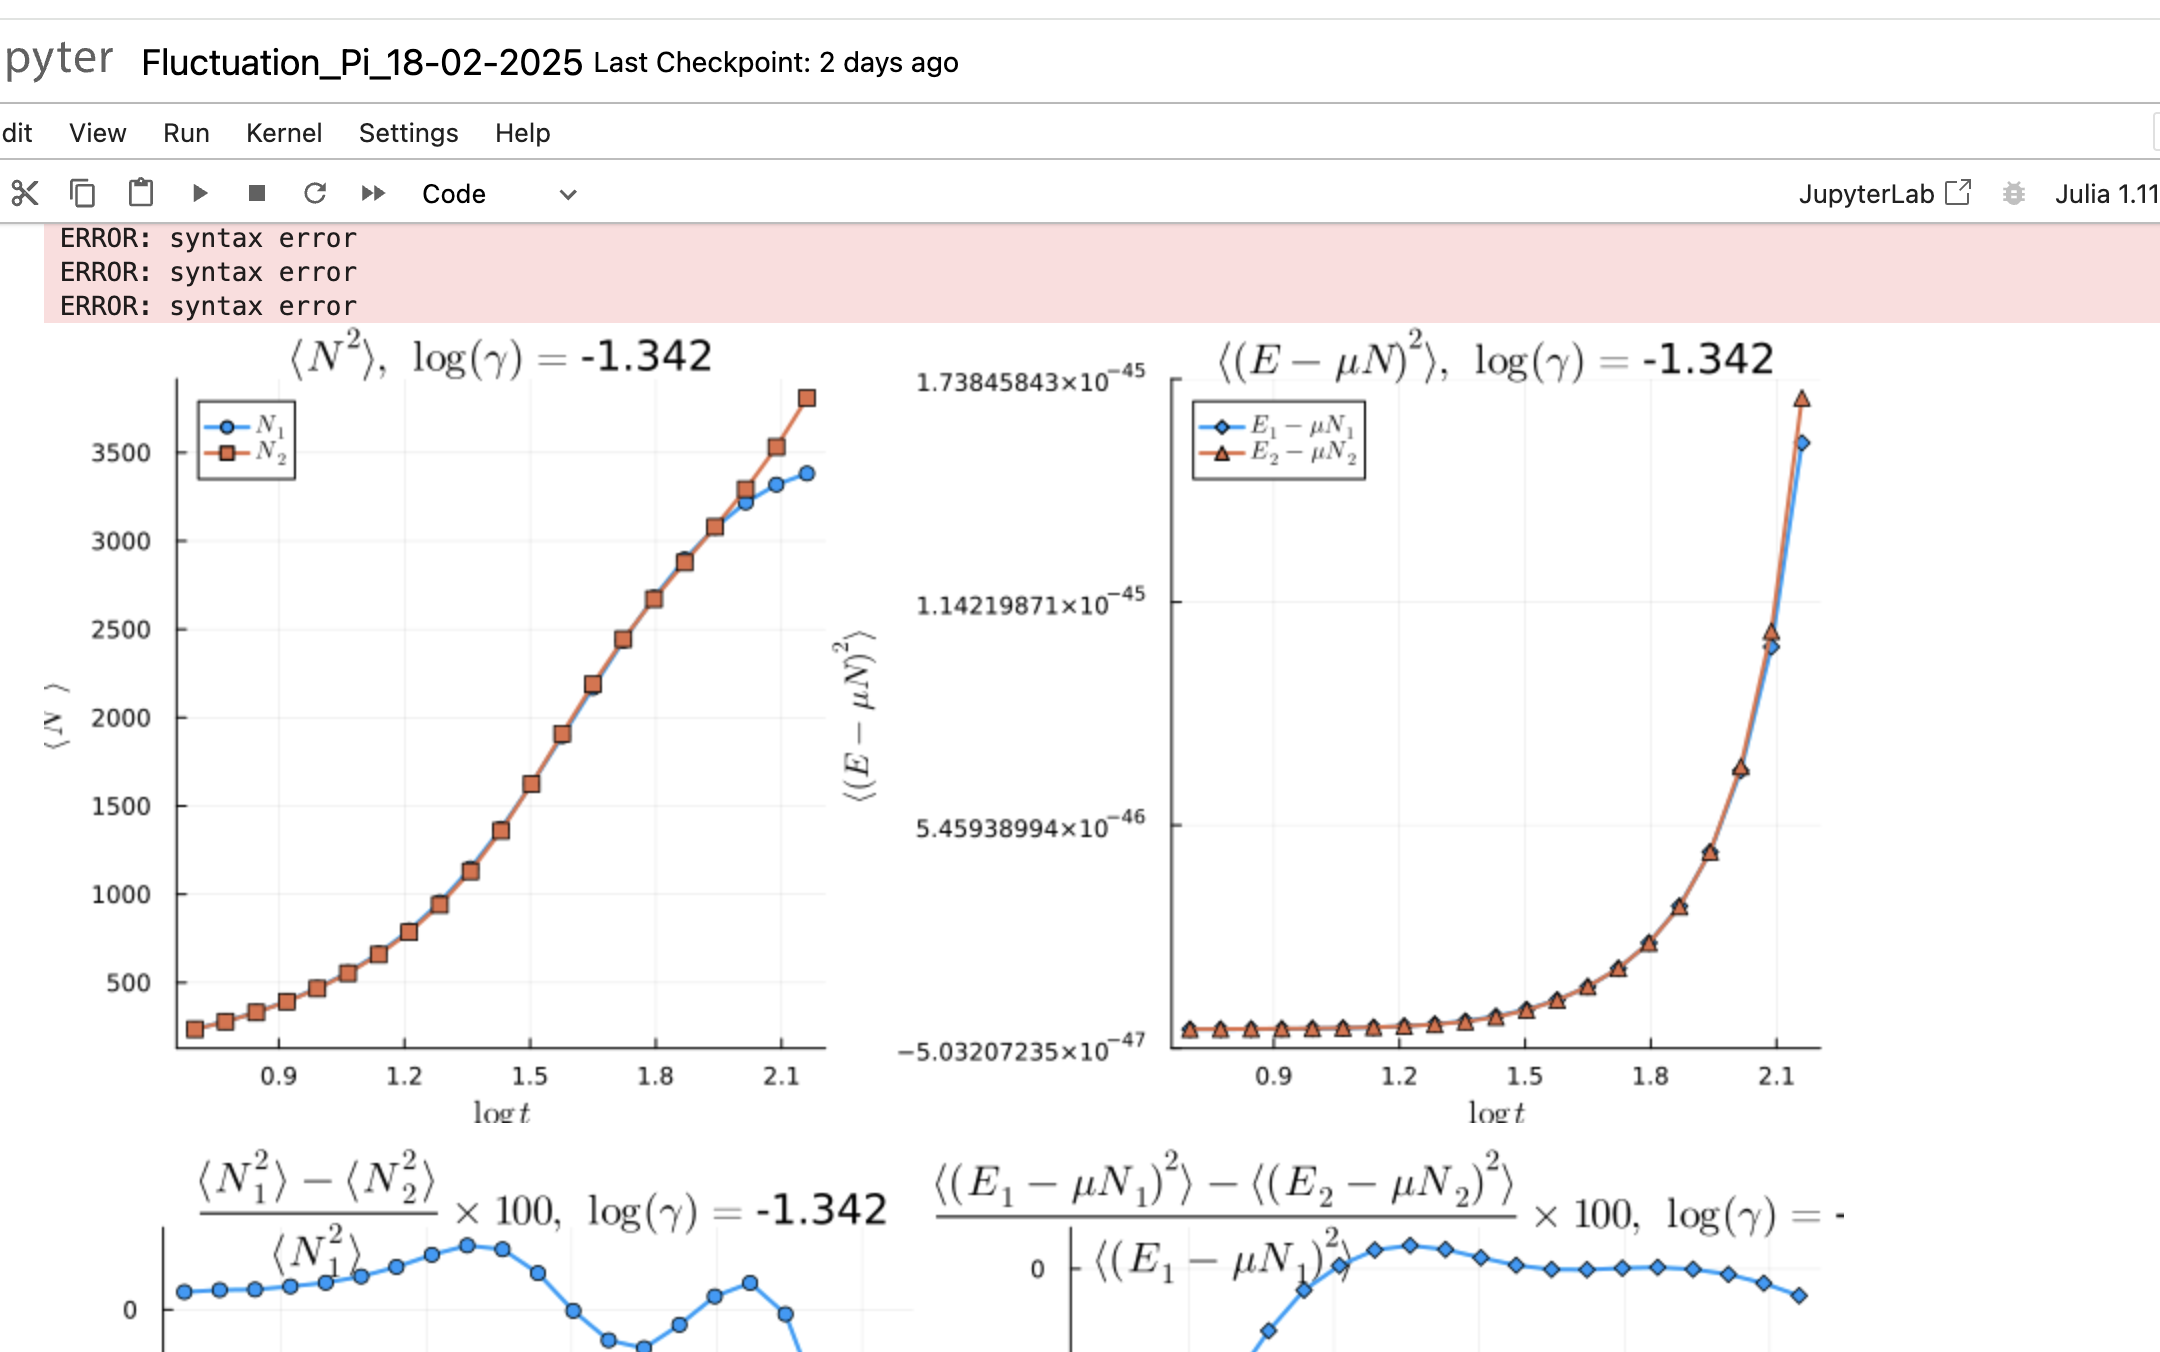
\includegraphics[width=1\textwidth]{Figures/test}

%\begin{aff}
%Donc une a l'ordre un en $\delta \theta (\operator{A}^{(0)})^{-1} %\operator{V}$ 

%\begin{eqnarray*}
%	\langle \delta \Pi ( \theta) \delta \Pi ( \theta') \rangle & = &  ( (\Pi^c_s - \Pi^c)\Pi^c/\Pi^c_s ) ( \theta ) \delta_{\theta, \theta'}/\delta \theta + \mathscr{F}(\theta , \theta' ) ,	
%\end{eqnarray*}

%avec 

%\begin{eqnarray*}
%	\mathscr{F}(\theta , \theta' ) & = & \left [ (\Pi^c_s - \Pi^c )( \theta)  +  (\Pi^c_s - \Pi^c ) ( \theta' )\right ] \frac{\Pi^c}{\Pi^c_s}(\theta)\frac{\Pi^c}{\Pi^c_s}(\theta') \frac{ \Delta( \theta'- \theta )}{ 2 \pi }\\
%	&&  - \left [ (\Pi^c_s - \Pi^c )( \theta)   (\Pi^c_s - \Pi^c ) ( \theta' )\right ] \frac{\Pi^c}{\Pi^c_s}(\theta)\frac{\Pi^c}{\Pi^c_s}(\theta')\int d\theta'' \left (   \frac{ \Pi^c/\Pi^c_s}{\Pi^c_s - \Pi^c} \right )(\theta'') \frac{\Delta(\theta''- \theta)}{2 \pi}\frac{\Delta(\theta''- \theta')}{2 \pi}  	
%\end{eqnarray*}
%\end{aff}



 








 
\subsection{Fonction d’onde et Hamiltonien et moment à N corps}
%%Dans ce chapitre, nous nous intéressons aux fluctuations de la distribution de rapidité \( \delta \rho \) autour d'une distribution de référence \( \rho^c \), qui maximise la contribution à la fonction de partition des états, exprimée comme une fonctionnelle de la distribution \( \rho \) : 

La fonction de partition des états, s'exprime comme une fonctionnelle de la distribution \( \rho \) : 

\begin{eqnarray*}
	\Xi & = & \sum_\rho \exp \left( -\mathcal{A}(\rho) \right).
\end{eqnarray*}  

Dans la section {\em \bf Entropie de Yang-Yang} (\ref{??}), l'action \( \mathcal{A}(\rho) \) s'écrit sous la forme :  

\begin{eqnarray*}
	\mathcal{A}(\rho) & \doteq & - L\mathcal{S}_{YY}(\rho) + L\int f(\theta) \rho (\theta) \, d\theta,		
\end{eqnarray*}  

où \( \mathcal{S}_{YY} \) est la fonctionnelle d'entropie de Yang-Yang, définie dans (\ref{??}), et \( f \) est la fonction paramétrant les charges, introduite dans (\ref{??}).  

Dans cette même section {\em \bf Entropie de Yang-Yang} (\ref{??}), nous avons établi un lien entre \( f \) et distribution de référence \( \rho^c \), qui maximise la contribution à la fonction de partition des états .\\

On veux tester si nos experience est décrit pas un GGE. Pour cela nous nous intéressons aux fluctuations de la distribution de rapidité \( \delta \rho \) autour \( \rho^c \).

%Nous poursuivons à présent avec cette définition de l'action de classe $\mathcal{C}^2$ et admetant une distribution critique $\rho^c$ tel que sa différentielle en ce point critique soit nulle $d\mathcal{A}_{\rho^c} = 0 $ (\ref{??}) de sorte que d'aprés la formule de Taylor-Youg %afin de déterminer les fluctuations autour de \( \Pi^c \). Pour cela, nous réécrivons l'action sous la forme :  

Nous poursuivons à présent avec cette définition de l'action de classe $\mathcal{C}^2$ et admetant une distribution critique $\rho^c$ tel que sa différentielle en ce point critique soit nulle $d\mathcal{A}_{\rho^c} = 0 $ (\ref{??}) de sorte que d'aprés la formule de Taylor-Youg %afin de déterminer les fluctuations autour de \( \Pi^c \). Pour cela, nous réécrivons l'action sous la forme :  

\begin{eqnarray*}  
	\mathcal{A}(\rho^c + \delta \rho) & \underset{ \delta \rho \to 0 }{=} & \mathcal{A}(\rho^c)  + \frac{1}{2} \left. \frac{\delta^2 \mathcal{A}}{\delta \rho^2} \right|_{\rho^c} (\delta \rho) + \mathcal{O}((\delta \rho)^3),  
\end{eqnarray*}  

une expression quadratique pour l'action à l'ordre dominant en \( \delta \Pi \) avec $\left. \frac{\delta^2 \mathcal{A}}{\delta \rho^2} \right|_{\rho^c}$ la forme quadratique définie positive (Fig (\ref{fig.fluctu.A})).

\begin{figure}[H]
	\centering 
	\begin{tikzpicture}
		\begin{scope}[shift={(0,0)}]
			\begin{scope}[transform canvas={scale=0.6}]
				% Définition des couleurs avec les codes HTML
\definecolor{colorOne}{HTML}{443E46}
\definecolor{colorTwo}{HTML}{F6DEB8}
\definecolor{colorThree}{HTML}{908CA4}
\definecolor{colorFour}{HTML}{57659E}
\definecolor{colorFive}{HTML}{C57284}
\definecolor{colorSix}{HTML}{FF5B69}

% Raccourcis pour les couleurs
\def\colorOne{colorOne}
\def\colorTwo{colorTwo}
\def\colorThree{colorThree}
\def\colorFour{colorFour}
\def\colorFive{colorFive}
\def\colorSix{colorSix}

\def\colorslide{blue!50!black}



\begin{scope}
	% Tracer une courbe lisse entre des points
	\draw[shift={(0,0)} ,\colorOne]
		(-1 , 0 ) edge [thick,line width=0.8ex , ->,>=triangle 45  , \colorOne] node [pos = 1 , below ]{\huge$\rho$}( 5  , 0 )
	;
	\draw[shift={(0,0)}, color=\colorOne]
		(0, -1.0 ) edge [thick,line width=0.8ex , ->,>=triangle 45  ]node [pos=0.9,left=0.2cm ]{\huge$\mathcal{A}(\rho)$}( 0  , 5 )
	;
	\draw[]
		(2.5, 0.12 ) edge [thick,line width=0.8ex ,\colorThree ]node [pos=1,below  ]{\huge$\rho^c$} (2.5, -0.12 )	
	;
	
	\draw[]
		(2.5, -0.12 ) edge [thick,line width=0.4ex , dashed, \colorThree ] (2.5, 5.5 )
		(1.5, 1 ) edge [thick,line width=0.4ex , <->,>=triangle 45  , \colorThree ] (3.5, 1 )
		(-0.3,1) edge [thick,line width=0.4ex  , \colorThree ] node [pos=0,left ]{\huge$\mathcal{A}(\rho^c)$} (0.3, 1 )	
	;
    \draw[thick, line width=0.8ex , \colorFour] plot[smooth, tension=0.7] coordinates {
        (1, 5) (1.6 , 3 ) (2.5, 1) (3.5 , 3 )  (4, 5)
    };		
	
\end{scope}

	
			
			\end{scope}
			
			\draw[color = red , scale = 0.5 , draw = none  ] (-2 , -1) rectangle (5, 6) ; 	
		\end{scope}
		
		\begin{scope}[shift={(19,-1)}]
			\begin{scope}[transform canvas={scale=0.6}]
				% Définition des couleurs avec les codes HTML
\definecolor{colorOne}{HTML}{443E46}
\definecolor{colorTwo}{HTML}{F6DEB8}
\definecolor{colorThree}{HTML}{908CA4}
\definecolor{colorFour}{HTML}{57659E}
\definecolor{colorFive}{HTML}{C57284}
\definecolor{colorSix}{HTML}{FF5B69}

% Raccourcis pour les couleurs
\def\colorOne{colorOne}
\def\colorTwo{colorTwo}
\def\colorThree{colorThree}
\def\colorFour{colorFour}
\def\colorFive{colorFive}
\def\colorSix{colorSix}

\def\colorslide{blue!50!black}

\def\Occupation{
	\def\traitx{0.3}
	\def\traity{0.5}
	\draw[shift={(0,0)}]
		(-13.5 , 0 ) edge [thick,line width=0.8ex ]( -3.2  , 0 )
		( -3.2 - \traitx  , 0 - \traity ) edge [thick,line width=0.8ex ]( -3.2 + \traitx  , 0 + \traity  )
		( -2.8 - \traitx  , 0 - \traity ) edge [thick,line width=0.8ex ]( -2.8 + \traitx  , 0 + \traity  )
		(-2.8 , 0 ) edge [thick,line width=0.8ex ](2.8  , 0 )
		( 2.8 - \traitx  , 0 - \traity ) edge [thick,line width=0.8ex ]( 2.8 + \traitx  , 0 + \traity  )
		( 3.2 - \traitx  , 0 - \traity ) edge [thick,line width=0.8ex ]( 3.2 + \traitx  , 0 + \traity  )
		(3.2, 0 ) edge [thick,line width=0.8ex,->,>=triangle 45 , color = black ]node [pos=1.01,below  ]{\huge$\theta$}	( 13  , 0 )
	;
	\draw[shift={(0,0)}, color=\colorOne]
		(-10.5 , -1.5 ) edge [thick,line width=0.8ex , ->,>=triangle 45  ]( -10.5  , 4.5 )
	;
		
	\foreach \r in {1 , ... , 3 } {
%		\draw[
%		decoration={
%		markings,
%    	mark connection node=my node,
%    	mark=at position 0 with{\node [blue,transform shape] (my node) {\large \r};}},
%		color=gray, thick, 
%		line width=0.5ex] decorate { 
%            (-11.0, \r) -- (-10.1, \r )}
%        ;
        \draw[
			color=\colorOne,
			] 
            (-11.0, \r) edge[color=\colorThree , thick,line width=0.5ex] node [pos=-0.5 ]{\large\color{\colorFour} $\frac{\r}{\delta \theta}$ } (-10.3, \r )
        	;
	
	}
	

	
	% Graduation abcsisse 
	% Définitions des listes
% Definitions of the lists
\def\listetuple{-9/\theta_{1}, -8/\theta_{2} , -5/\theta_{3} , -2/\theta_{a-1} , 0/\theta_{a} , 1/\theta_{a+1} , 2/\theta_{a+2} ,  5/\theta_{N-4} , 7/\theta_{N-3},8/\theta_{N-1},9/\theta_{N} }
\def\listetrais{-12 , -11, -10, -9 , -8 , -7 ,  -6 , -5, -4.5,-4, -2 , -1, 0 , 0.5, 1, 2, 4 , 5 ,  6 , 7 , 8 ,8.5, 9 ,  10 , 11, 12 }

% Loop over listetrais
\foreach \r in \listetrais {
    % Initialize found variable to zero
    % Initialize found variable to zero
    %\pgfmathsetmacro\found{0}
    \global\def\found{0}
    \xdef\nomtheta{}
    
    % Check if \r is in listetuple
    \foreach \x/\y in \listetuple { 
        \ifdim \r pt=\x pt % If \r matches any \x in listetuple
            \global\def\found{1} ;
            \xdef\nomtheta{\y} % Set \nomtheta to the corresponding \y
            %\pgfmathsetmacro\found{1} % Set found to 1            
            %\global\pgfmathsetmacro\found{1}
        \fi
    }
    
    %\node [circle, draw, red] (A) at (\r, 2) {\found , $\nomtheta$};
    
    % Draw the line and display \nomtheta if found
    \ifnum\found=1
        \draw[color=\colorOne, thick, line width=0.5ex] 
            (\r, -0.3) -- (\r, 0.3) node[red , pos=-0.5] {\large $\nomtheta$};
         \filldraw[line width=0.5ex, color=\colorSix, outer color=\colorSix, inner color=\colorSix] 
            (\r, 0) circle (4pt);
    \else 
        % Draw without \nomtheta and add a blue circle if not found
        \draw[color=\colorOne, thick, line width=0.5ex] 
            (\r, -0.3) -- (\r, 0.3);
        \filldraw[line width=0.5ex, color=\colorSix, outer color=\colorTwo, inner color=\colorTwo] 
            (\r, 0) circle (4pt); 
    \fi
}

\def\listetrais{-9.5/\theta_{i-1}/2/3, -6.5/\theta_{i}/1/4  ,   -1.5/\theta_{j}/2/4 , 1.5/\theta_{j+1}/-1/3 , 3.5/\theta_{\ell-1}/1/3 , 6.5/\theta_{\ell}/3/4 , 9.5/\theta(\theta_{\ell+1})/-1/3 };



\foreach \r/\nomx/\y/\ys in \listetrais {
	\draw[
		decoration={
		markings,
    	mark connection node=my node,
    	mark=at position .5 with{\node [blue,transform shape] (my node) {\large \color{\colorFour} $\nomx$};}},
		color=\colorThree , thick, 
		line width=0.5ex] decorate { 
            (\r, 0.12) -- (\r, -1.2)}
        ;
     
     \ifdim \y pt > -1 pt 
     	\draw[
			decoration={
			markings,
    		mark connection node=my node,
    		mark=at position .5 with{\node [blue,transform shape] (my node) {\large \color{\colorFour} $\Pi(\nomx) $};}},
			color=\colorThree, thick, 
			line width=0.5ex] decorate { 
            (\r, \y) -- (\r +3, \y)}
        ;
        \draw[
			decoration={
			markings,
    		mark connection node=my node,
    		mark=at position .5 with{\node [blue,transform shape] (my node) {\large \color{\colorFive} $\Pi_s(\nomx) $};}},
			color=\colorFive, thick, 
			line width=0.5ex] decorate { 
            (\r, \ys) -- (\r +3, \ys)}
        ;
     \fi 
     \ifdim \r pt= -1.5 pt
     	\draw[
     		decoration={
			markings,
    		mark connection node=my node,
    		mark=at position .5 with{\node [blue,transform shape] (my node) {\large \color{\colorFour}  $\delta \theta $};},
    		%mark=at position 0.1  with {\arrow[blue, line width=0.5ex]{<}},
    		%mark=at position 1  with {\arrow[blue, line width=0.5ex]{>}}
    		},
        	color=\colorThree,
        	thick,
        	line width=0.5ex,
        	%arrows={Computer Modern Rightarrow[line cap=round]-Computer Modern Rightarrow[line cap=round]}
   			](\r, -1.2) edge[arrows={Computer Modern Rightarrow[line cap=round]-}] (\r + 0.4, -1.2)decorate {
    		(\r, -1.2) -- (\r + 3, -1.2)}(\r + 2, -1.2) edge[arrows={-Computer Modern Rightarrow[line cap=round]}] (\r + 3, -1.2)
    		;
    \fi
			
	
}


			
}


\begin{scope}
	%\draw[help lines , width=1.5ex] (-8,-3) grid (8,3);\draw[help lines ,width=0.5ex , opacity = 0.5] (-3,-3) grid[step=0.1] (3,3));
	
	%\draw[help lines] 
	%	(-3,-3) edge[width=1.5ex] grid (3,3)	
	%	(-3,-3) edge[width=0.5ex , opacity = 0.5] grid (3,3)	
	%;
	\begin{scope}[shift={(0,1)},rotate=0,opacity=1,color=black]
		\Occupation	
		
		%\node[anchor=east, font=\bfseries] at (-11, 0) {\color{red}\large (T = 0 )} ;	
	\end{scope}
	
	
	
	
	\begin{scope}[shift={(-10.5,7)},rotate=0,opacity=1,color=black]
	
	\begin{scope}[shift={(-0,0)},rotate=0,opacity=1,color=black]
	
		\draw[shift={(0,0)} ,line width=1ex,rounded corners = 1ex,color=\colorOne , opacity =1 ,fill=\colorOne!00 , pattern={north east lines} , pattern color=\colorOne!00 ]
			(0 , -1 ) rectangle (5,1)
		;
		

		\begin{scope}[shift={(0.5,0.5)}]
			\draw[color=\colorOne, thick, line width=0.5ex] 
            (0, -0.3) -- (0, 0.3) ;
            \filldraw[line width=0.5ex, color=\colorSix, outer color=\colorSix, inner color=\colorSix] 
            (0, 0) circle (4pt);
            
            \node[anchor=west, font=\bfseries] at (0.2, 0) {\color{\colorSix}\large : quasi-particule};
		\end{scope}
		
		\begin{scope}[shift={(0.5,-0.5)}]
			\draw[color=\colorOne, thick, line width=0.5ex] 
            (0, -0.3) -- (0, 0.3) ;
            \filldraw[line width=0.5ex, color=\colorSix, outer color=\colorTwo, inner color=\colorTwo] 
            (0, 0) circle (4pt);
            
            \node[anchor=west, font=\bfseries] at (0.2, 0) {\color{\colorSix}\large : hole};
		\end{scope}

	\end{scope}
	
	\begin{scope}[shift={(6,0)},rotate=0,opacity=1,color=black]	
		
		\draw[shift={(0,0)} ,line width=1ex,rounded corners = 1ex,color=\colorOne , opacity =1 ,fill=\colorOne!00 , pattern={north east lines} , pattern color=\colorOne!00 ]
			(0 , -1 ) rectangle (7.5,1)
		;
		
		\node[anchor=west] at (0.5, 0.5) {\color{\colorFour}\large $\Pi$ };\node[anchor=west, font=\bfseries] at (1, 0.5) {\color{\colorFour}\large : quasi-particule distribution};
		
		\node[anchor=west] at (0.5, -0.5) {\color{\colorFour}\large $\Pi_h$ };\node[anchor=west, font=\bfseries] at (1, -0.5) {\color{\colorFour}\large  : hole distribution};
		
	\end{scope}
	
	\begin{scope}[shift={(14.5,0)},rotate=0,opacity=1,color=black]	
		
		\draw[shift={(0,0)} ,line width=1ex,rounded corners = 1ex,color=\colorOne , opacity =1 ,fill=\colorOne!00 , pattern={north east lines} , pattern color=\colorOne!00 ]
			(0 , -0.5 ) rectangle (7.0,0.5)
		;
		
		\node[anchor=west] at (0.2, 0) {\color{\colorFour}\large ${\color{\colorFive}\Pi_s} = \Pi + \Pi_h $ } node[anchor=west , font=\bfseries] at (3.1 , 0 )  {\color{\colorFour}\large {\color{\colorFive} : density of states}};
		
	\end{scope}
	
	
	\end{scope}


		
	
\end{scope}

	
			
			\end{scope}
			\begin{scope}[scale=1]
				\draw[color = red , scale = 1 , draw = none  ] (-1 , -1) rectangle (5, 5) ; 
			\end{scope}	
		\end{scope}

		
				
			
	\end{tikzpicture}	
	\captionsetup{skip=10pt} % Ajoute de l’espace après la légende
	\label{fig.fluctu.A}
\end{figure}


On discrétise l'axe des rapidités en  petite cellule de rapidité $[\theta, \theta+\delta\theta]$, qui contient $L\rho(\theta) \delta \theta$ rapidités. 
	



Avec ces petites tranches, la forme quadratique s’écrit :

\begin{eqnarray*}
    \left. \frac{\delta^2 \mathcal{A}}{{\delta \rho}^2} \right|_{\rho^c}(\delta \rho ) &=&  \sum_{a,b \mid \text{tranche}}  
    \delta \rho(\theta_a)  \frac{\partial^2 \mathcal{A}}{\partial \delta \rho(\theta_a) \partial \delta \rho(\theta_b) } (\rho^c)  \delta \rho(\theta_b).
\end{eqnarray*}
Les fluctuations s’écrivent donc :

\begin{eqnarray*}
    \langle \delta \rho ( \theta) \delta \rho ( \theta') \rangle &=&  
    \frac{ \int d\delta \rho \, \delta \rho(\theta) \delta \rho ( \theta') 
    \exp \left( - \frac{1}{2} \sum_{a,b \mid \text{tranche}}  
    \delta \rho(\theta_a) \frac{\partial^2 \mathcal{A}}{\partial \delta \rho(\theta_a) \partial \delta \rho(\theta_b) } (\rho^c)  \delta \rho(\theta_b) \right) }
    { \int d\delta \Pi  
    \exp \left( - \frac{1}{2} \sum_{a,b \mid \text{tranche}}  
    \delta \rho(\theta_a) \frac{\partial^2 \mathcal{A}}{\partial \delta \rho(\theta_a) \partial \delta \rho(\theta_b) } (\rho^c)  \delta \rho(\theta_b) \right) } \\
    &=& \left( \mathbf{A}^{-1} \right)_{\theta , \theta'}
\end{eqnarray*}


\begin{aff}

\begin{eqnarray*}
	\langle \delta \rho ( \theta) \delta \rho ( \theta') \rangle &=& 	\left( \mathbf{A}^{-1} \right)_{\theta , \theta'}
\end{eqnarray*}

	
avec la  {\em matrice hessienne} $\mathbf{A}_{\theta , \theta'} \equiv \frac{\partial^2 \mathcal{A}}{\partial \delta \rho(\theta) \partial \delta \rho(\theta') }(\rho^c)$, au point critique/ qui maximise la probabilité  $\rho^c=\rho^c_s \nu^c $, s'écrit

\begin{eqnarray*}
	\operator{A} & = & \operator{A}^{(0)} + \delta \theta \operator{V}
\end{eqnarray*}

avec 

\begin{eqnarray*}
	A^{(0)}_{\theta , \theta'}  & = &  L\delta \theta \left ( \frac{ 1}{\rho^c_s ( 1  - \nu^c ) \nu^c } \right )(\theta)    \delta({\theta - \theta '})	,\\
	V_{\theta , \theta'}  &= & L \delta \theta \left \{ - \left [ \left ( \frac{1}{\rho^c_s( 1 - \nu^c) } \right ) ( \theta)  +  \left ( \frac{1}{\rho^c_s( 1 - \nu^c) } \right ) ( \theta' )\right ] \frac{ \Delta( \theta'- \theta )}{ 2 \pi } + \int d\theta''  \left ( \frac{\nu^c}{\rho^c_s( 1 - \nu^c) } \right )(\theta'') \frac{\Delta(\theta''- \theta)}{2 \pi}\frac{\Delta(\theta''- \theta')}{2 \pi}   \right \} 	
\end{eqnarray*}

\end{aff}

\subsection{Testes}

\begin{eqnarray*}
	\Delta_{\operator{\mathcal{N}}}^2  & = &  \frac{1}{\beta} \left . \frac{\partial \langle \operator{\mathcal{N}} \rangle}{\partial \mu} \right )_T \\
	\Delta_{\operator{\mathcal{E}}-\mu \operator{\mathcal{N}}}^2  & = &  - \left . \frac{\partial \langle \operator{\mathcal{E}}-\mu \operator{\mathcal{N}} \rangle}{\partial \beta} \right )_\mu 
\end{eqnarray*}

et 

\begin{eqnarray*}
	\Delta_{\operator{\mathcal{N}}}^2  &= & L^2 \int d\theta_a \int d \theta_b \, \langle \delta \rho(\theta_a) \delta \rho(\theta_b) \rangle \\
	\Delta_{\operator{\mathcal{E}}-\mu \operator{\mathcal{N}}}^2  & = & L^2 \int d\theta_a \int d \theta_b \, \left ( - \mu + \frac{1}2 m \theta_a^2  \right  )\left ( - \mu + \frac{1}2 m \theta_b^2  \right  )  \langle \delta \rho(\theta_a) \delta \rho(\theta_b) \rangle
\end{eqnarray*}

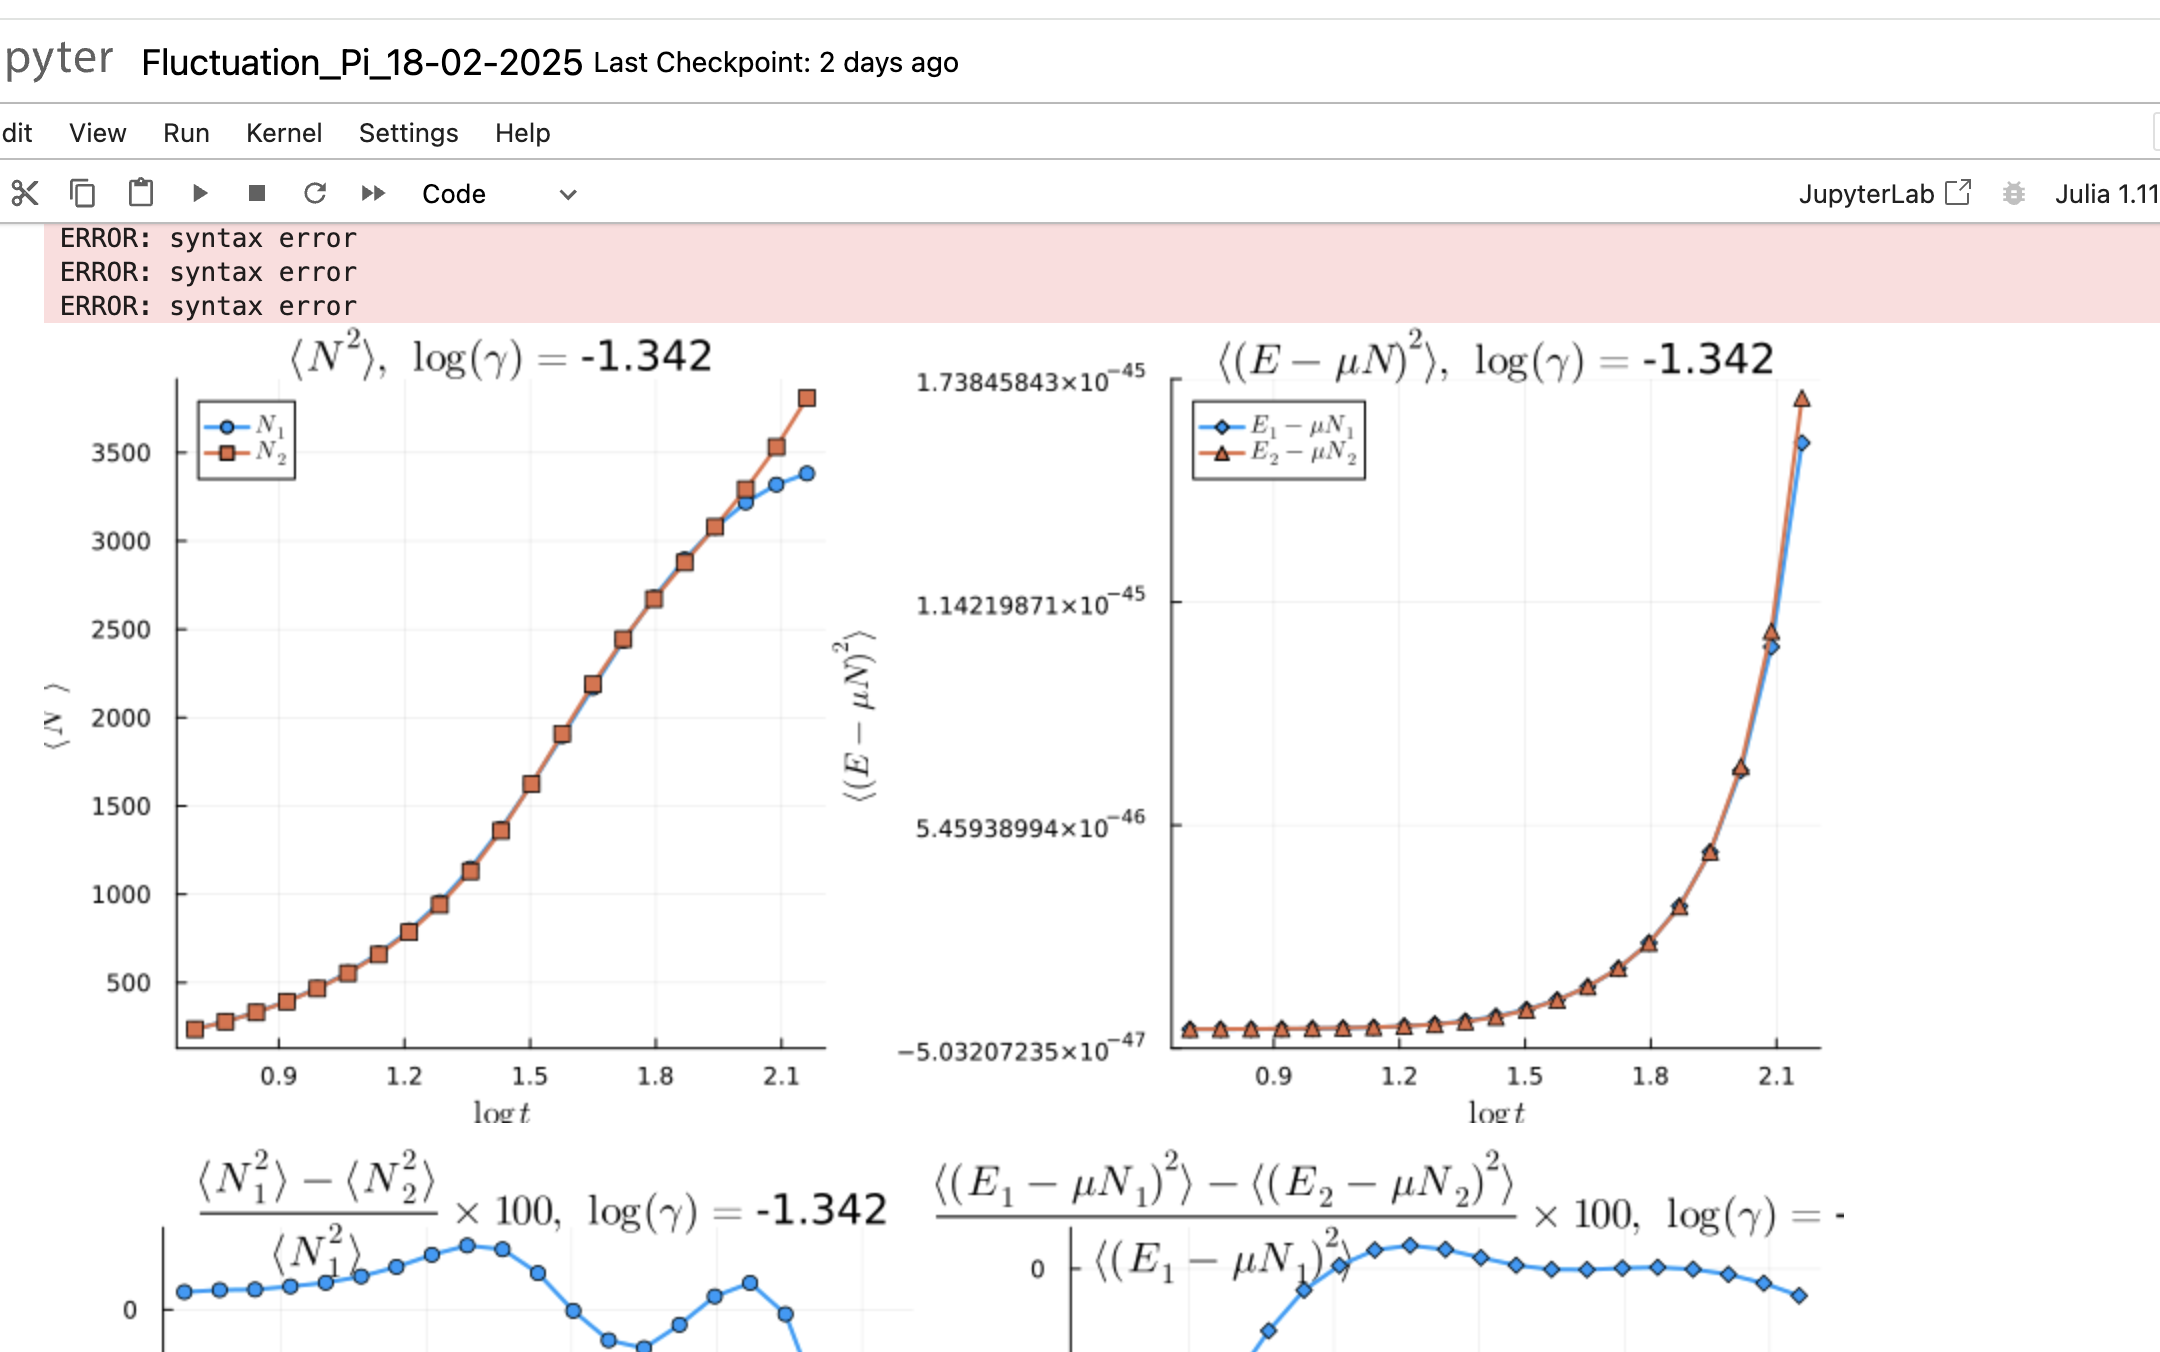
\includegraphics[width=1\textwidth]{Figures/test}

%\begin{aff}
%Donc une a l'ordre un en $\delta \theta (\operator{A}^{(0)})^{-1} %\operator{V}$ 

%\begin{eqnarray*}
%	\langle \delta \Pi ( \theta) \delta \Pi ( \theta') \rangle & = &  ( (\Pi^c_s - \Pi^c)\Pi^c/\Pi^c_s ) ( \theta ) \delta_{\theta, \theta'}/\delta \theta + \mathscr{F}(\theta , \theta' ) ,	
%\end{eqnarray*}

%avec 

%\begin{eqnarray*}
%	\mathscr{F}(\theta , \theta' ) & = & \left [ (\Pi^c_s - \Pi^c )( \theta)  +  (\Pi^c_s - \Pi^c ) ( \theta' )\right ] \frac{\Pi^c}{\Pi^c_s}(\theta)\frac{\Pi^c}{\Pi^c_s}(\theta') \frac{ \Delta( \theta'- \theta )}{ 2 \pi }\\
%	&&  - \left [ (\Pi^c_s - \Pi^c )( \theta)   (\Pi^c_s - \Pi^c ) ( \theta' )\right ] \frac{\Pi^c}{\Pi^c_s}(\theta)\frac{\Pi^c}{\Pi^c_s}(\theta')\int d\theta'' \left (   \frac{ \Pi^c/\Pi^c_s}{\Pi^c_s - \Pi^c} \right )(\theta'') \frac{\Delta(\theta''- \theta)}{2 \pi}\frac{\Delta(\theta''- \theta')}{2 \pi}  	
%\end{eqnarray*}
%\end{aff}



 








\subsection{Introduction au modèle de gaz de Bose unidimensionnel}
%Dans ce chapitre, nous nous intéressons aux fluctuations de la distribution de rapidité \( \delta \rho \) autour d'une distribution de référence \( \rho^c \), qui maximise la contribution à la fonction de partition des états, exprimée comme une fonctionnelle de la distribution \( \rho \) : 

La fonction de partition des états, s'exprime comme une fonctionnelle de la distribution \( \rho \) : 

\begin{eqnarray*}
	\Xi & = & \sum_\rho \exp \left( -\mathcal{A}(\rho) \right).
\end{eqnarray*}  

Dans la section {\em \bf Entropie de Yang-Yang} (\ref{??}), l'action \( \mathcal{A}(\rho) \) s'écrit sous la forme :  

\begin{eqnarray*}
	\mathcal{A}(\rho) & \doteq & - L\mathcal{S}_{YY}(\rho) + L\int f(\theta) \rho (\theta) \, d\theta,		
\end{eqnarray*}  

où \( \mathcal{S}_{YY} \) est la fonctionnelle d'entropie de Yang-Yang, définie dans (\ref{??}), et \( f \) est la fonction paramétrant les charges, introduite dans (\ref{??}).  

Dans cette même section {\em \bf Entropie de Yang-Yang} (\ref{??}), nous avons établi un lien entre \( f \) et distribution de référence \( \rho^c \), qui maximise la contribution à la fonction de partition des états .\\

On veux tester si nos experience est décrit pas un GGE. Pour cela nous nous intéressons aux fluctuations de la distribution de rapidité \( \delta \rho \) autour \( \rho^c \).

%Nous poursuivons à présent avec cette définition de l'action de classe $\mathcal{C}^2$ et admetant une distribution critique $\rho^c$ tel que sa différentielle en ce point critique soit nulle $d\mathcal{A}_{\rho^c} = 0 $ (\ref{??}) de sorte que d'aprés la formule de Taylor-Youg %afin de déterminer les fluctuations autour de \( \Pi^c \). Pour cela, nous réécrivons l'action sous la forme :  

Nous poursuivons à présent avec cette définition de l'action de classe $\mathcal{C}^2$ et admetant une distribution critique $\rho^c$ tel que sa différentielle en ce point critique soit nulle $d\mathcal{A}_{\rho^c} = 0 $ (\ref{??}) de sorte que d'aprés la formule de Taylor-Youg %afin de déterminer les fluctuations autour de \( \Pi^c \). Pour cela, nous réécrivons l'action sous la forme :  

\begin{eqnarray*}  
	\mathcal{A}(\rho^c + \delta \rho) & \underset{ \delta \rho \to 0 }{=} & \mathcal{A}(\rho^c)  + \frac{1}{2} \left. \frac{\delta^2 \mathcal{A}}{\delta \rho^2} \right|_{\rho^c} (\delta \rho) + \mathcal{O}((\delta \rho)^3),  
\end{eqnarray*}  

une expression quadratique pour l'action à l'ordre dominant en \( \delta \Pi \) avec $\left. \frac{\delta^2 \mathcal{A}}{\delta \rho^2} \right|_{\rho^c}$ la forme quadratique définie positive (Fig (\ref{fig.fluctu.A})).

\begin{figure}[H]
	\centering 
	\begin{tikzpicture}
		\begin{scope}[shift={(0,0)}]
			\begin{scope}[transform canvas={scale=0.6}]
				\input{Figures/Fonc_A_code}	
			
			\end{scope}
			
			\draw[color = red , scale = 0.5 , draw = none  ] (-2 , -1) rectangle (5, 6) ; 	
		\end{scope}
		
		\begin{scope}[shift={(19,-1)}]
			\begin{scope}[transform canvas={scale=0.6}]
				\input{Figures/Occupation_theta_code}	
			
			\end{scope}
			\begin{scope}[scale=1]
				\draw[color = red , scale = 1 , draw = none  ] (-1 , -1) rectangle (5, 5) ; 
			\end{scope}	
		\end{scope}

		
				
			
	\end{tikzpicture}	
	\captionsetup{skip=10pt} % Ajoute de l’espace après la légende
	\label{fig.fluctu.A}
\end{figure}


On discrétise l'axe des rapidités en  petite cellule de rapidité $[\theta, \theta+\delta\theta]$, qui contient $L\rho(\theta) \delta \theta$ rapidités. 
	



Avec ces petites tranches, la forme quadratique s’écrit :

\begin{eqnarray*}
    \left. \frac{\delta^2 \mathcal{A}}{{\delta \rho}^2} \right|_{\rho^c}(\delta \rho ) &=&  \sum_{a,b \mid \text{tranche}}  
    \delta \rho(\theta_a)  \frac{\partial^2 \mathcal{A}}{\partial \delta \rho(\theta_a) \partial \delta \rho(\theta_b) } (\rho^c)  \delta \rho(\theta_b).
\end{eqnarray*}
Les fluctuations s’écrivent donc :

\begin{eqnarray*}
    \langle \delta \rho ( \theta) \delta \rho ( \theta') \rangle &=&  
    \frac{ \int d\delta \rho \, \delta \rho(\theta) \delta \rho ( \theta') 
    \exp \left( - \frac{1}{2} \sum_{a,b \mid \text{tranche}}  
    \delta \rho(\theta_a) \frac{\partial^2 \mathcal{A}}{\partial \delta \rho(\theta_a) \partial \delta \rho(\theta_b) } (\rho^c)  \delta \rho(\theta_b) \right) }
    { \int d\delta \Pi  
    \exp \left( - \frac{1}{2} \sum_{a,b \mid \text{tranche}}  
    \delta \rho(\theta_a) \frac{\partial^2 \mathcal{A}}{\partial \delta \rho(\theta_a) \partial \delta \rho(\theta_b) } (\rho^c)  \delta \rho(\theta_b) \right) } \\
    &=& \left( \mathbf{A}^{-1} \right)_{\theta , \theta'}
\end{eqnarray*}


\begin{aff}

\begin{eqnarray*}
	\langle \delta \rho ( \theta) \delta \rho ( \theta') \rangle &=& 	\left( \mathbf{A}^{-1} \right)_{\theta , \theta'}
\end{eqnarray*}

	
avec la  {\em matrice hessienne} $\mathbf{A}_{\theta , \theta'} \equiv \frac{\partial^2 \mathcal{A}}{\partial \delta \rho(\theta) \partial \delta \rho(\theta') }(\rho^c)$, au point critique/ qui maximise la probabilité  $\rho^c=\rho^c_s \nu^c $, s'écrit

\begin{eqnarray*}
	\operator{A} & = & \operator{A}^{(0)} + \delta \theta \operator{V}
\end{eqnarray*}

avec 

\begin{eqnarray*}
	A^{(0)}_{\theta , \theta'}  & = &  L\delta \theta \left ( \frac{ 1}{\rho^c_s ( 1  - \nu^c ) \nu^c } \right )(\theta)    \delta({\theta - \theta '})	,\\
	V_{\theta , \theta'}  &= & L \delta \theta \left \{ - \left [ \left ( \frac{1}{\rho^c_s( 1 - \nu^c) } \right ) ( \theta)  +  \left ( \frac{1}{\rho^c_s( 1 - \nu^c) } \right ) ( \theta' )\right ] \frac{ \Delta( \theta'- \theta )}{ 2 \pi } + \int d\theta''  \left ( \frac{\nu^c}{\rho^c_s( 1 - \nu^c) } \right )(\theta'') \frac{\Delta(\theta''- \theta)}{2 \pi}\frac{\Delta(\theta''- \theta')}{2 \pi}   \right \} 	
\end{eqnarray*}

\end{aff}

\subsection{Testes}

\begin{eqnarray*}
	\Delta_{\operator{\mathcal{N}}}^2  & = &  \frac{1}{\beta} \left . \frac{\partial \langle \operator{\mathcal{N}} \rangle}{\partial \mu} \right )_T \\
	\Delta_{\operator{\mathcal{E}}-\mu \operator{\mathcal{N}}}^2  & = &  - \left . \frac{\partial \langle \operator{\mathcal{E}}-\mu \operator{\mathcal{N}} \rangle}{\partial \beta} \right )_\mu 
\end{eqnarray*}

et 

\begin{eqnarray*}
	\Delta_{\operator{\mathcal{N}}}^2  &= & L^2 \int d\theta_a \int d \theta_b \, \langle \delta \rho(\theta_a) \delta \rho(\theta_b) \rangle \\
	\Delta_{\operator{\mathcal{E}}-\mu \operator{\mathcal{N}}}^2  & = & L^2 \int d\theta_a \int d \theta_b \, \left ( - \mu + \frac{1}2 m \theta_a^2  \right  )\left ( - \mu + \frac{1}2 m \theta_b^2  \right  )  \langle \delta \rho(\theta_a) \delta \rho(\theta_b) \rangle
\end{eqnarray*}

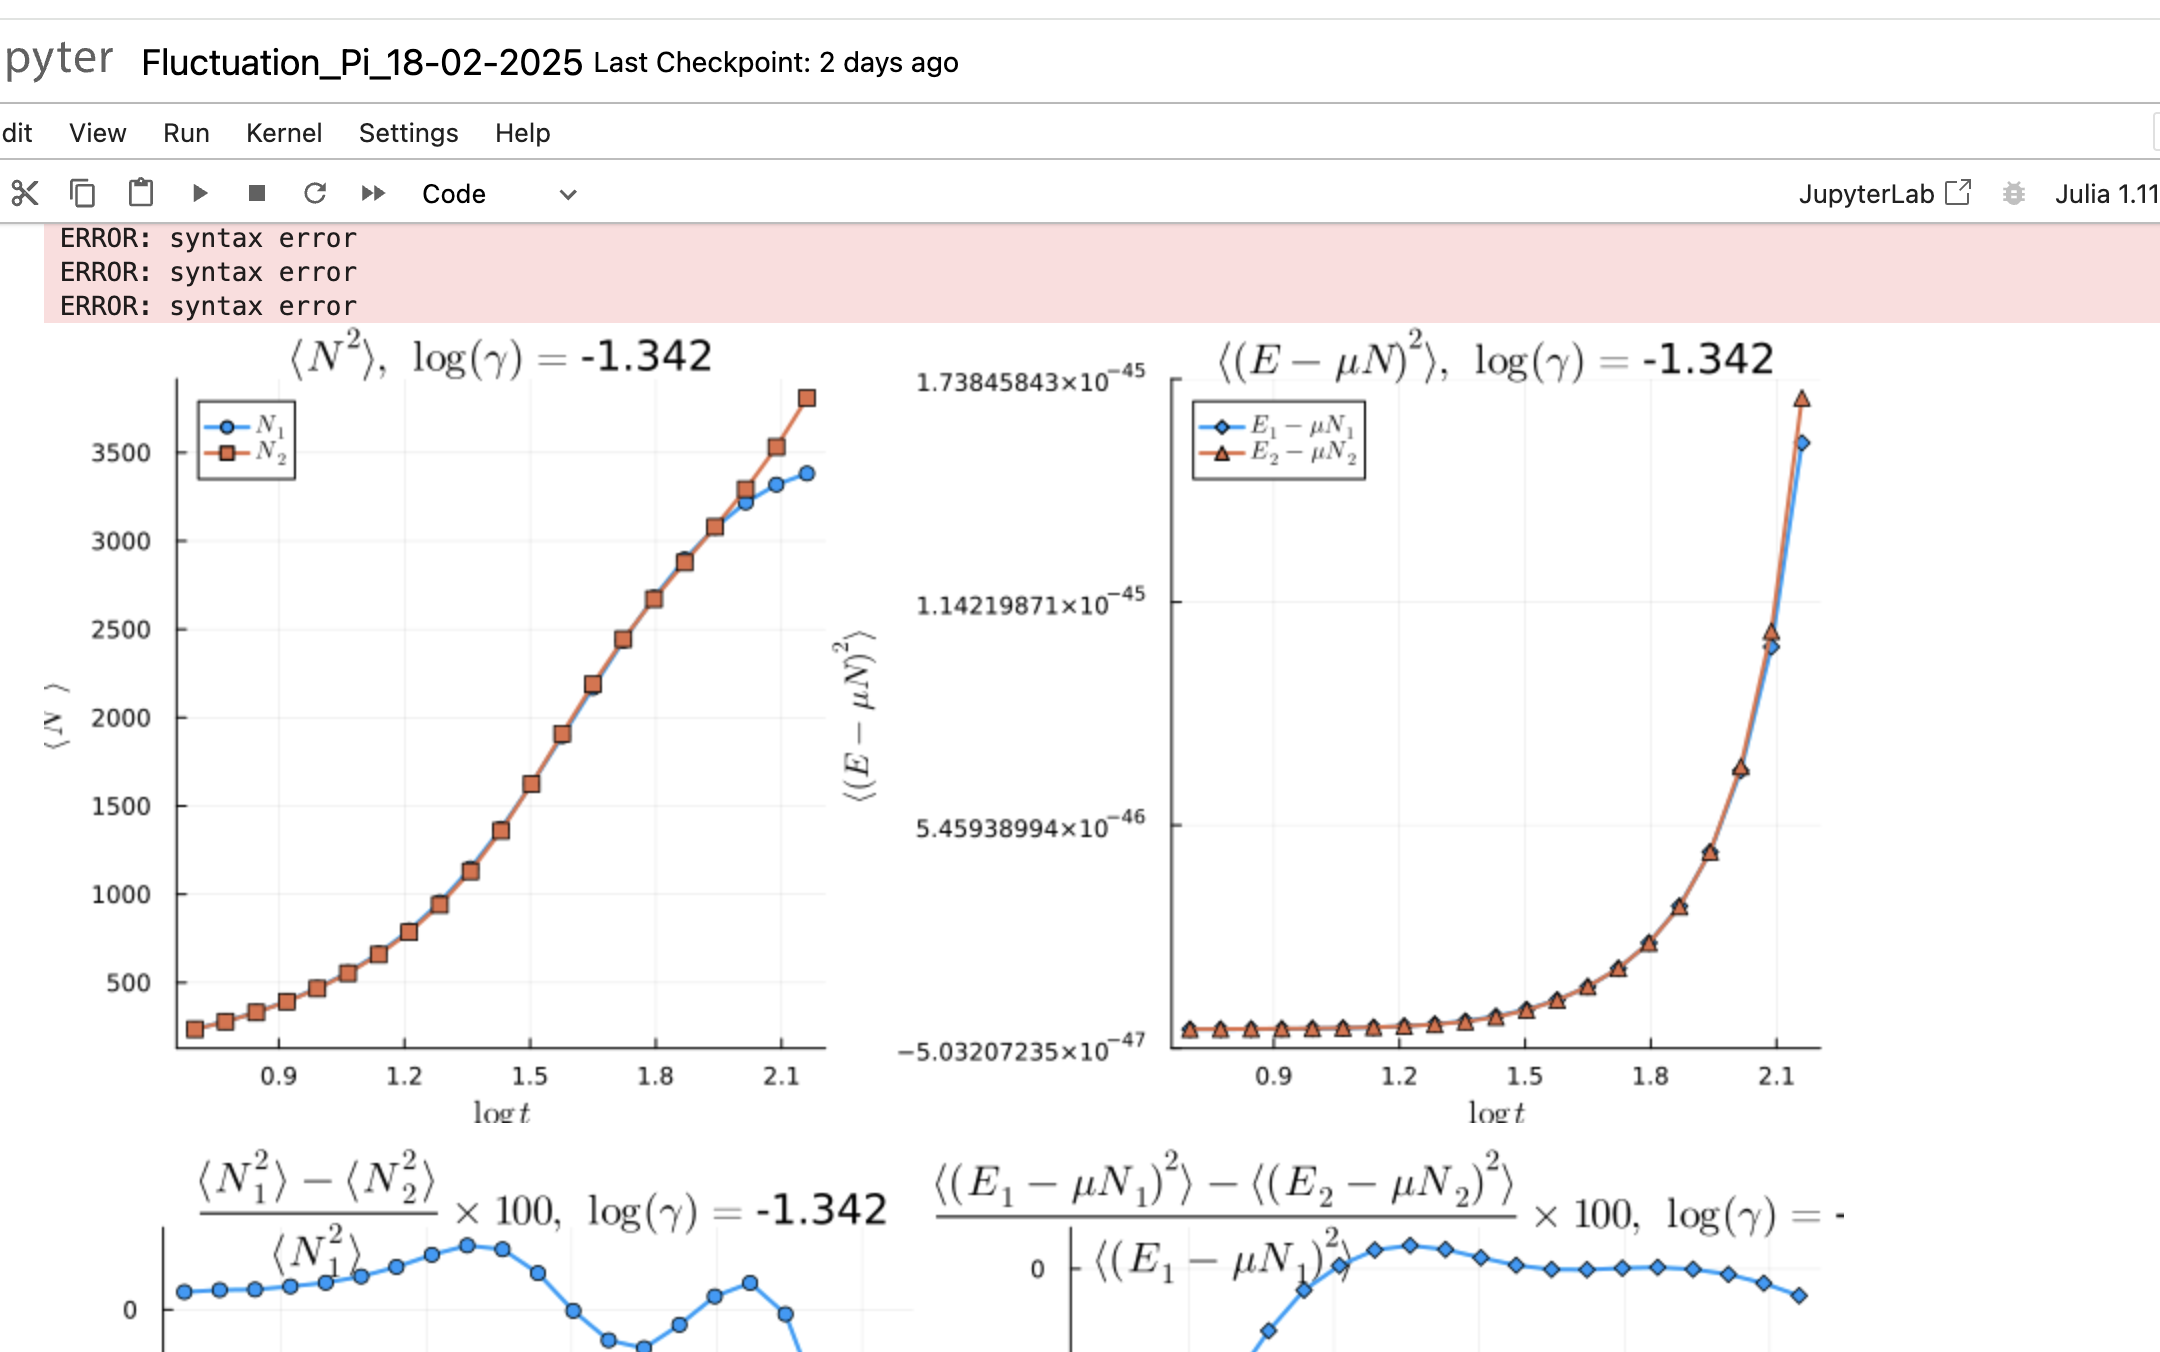
\includegraphics[width=1\textwidth]{Figures/test}

%\begin{aff}
%Donc une a l'ordre un en $\delta \theta (\operator{A}^{(0)})^{-1} %\operator{V}$ 

%\begin{eqnarray*}
%	\langle \delta \Pi ( \theta) \delta \Pi ( \theta') \rangle & = &  ( (\Pi^c_s - \Pi^c)\Pi^c/\Pi^c_s ) ( \theta ) \delta_{\theta, \theta'}/\delta \theta + \mathscr{F}(\theta , \theta' ) ,	
%\end{eqnarray*}

%avec 

%\begin{eqnarray*}
%	\mathscr{F}(\theta , \theta' ) & = & \left [ (\Pi^c_s - \Pi^c )( \theta)  +  (\Pi^c_s - \Pi^c ) ( \theta' )\right ] \frac{\Pi^c}{\Pi^c_s}(\theta)\frac{\Pi^c}{\Pi^c_s}(\theta') \frac{ \Delta( \theta'- \theta )}{ 2 \pi }\\
%	&&  - \left [ (\Pi^c_s - \Pi^c )( \theta)   (\Pi^c_s - \Pi^c ) ( \theta' )\right ] \frac{\Pi^c}{\Pi^c_s}(\theta)\frac{\Pi^c}{\Pi^c_s}(\theta')\int d\theta'' \left (   \frac{ \Pi^c/\Pi^c_s}{\Pi^c_s - \Pi^c} \right )(\theta'') \frac{\Delta(\theta''- \theta)}{2 \pi}\frac{\Delta(\theta''- \theta')}{2 \pi}  	
%\end{eqnarray*}
%\end{aff}



 









\subsection{Hamiltonien du modèle}
%Dans ce chapitre, nous nous intéressons aux fluctuations de la distribution de rapidité \( \delta \rho \) autour d'une distribution de référence \( \rho^c \), qui maximise la contribution à la fonction de partition des états, exprimée comme une fonctionnelle de la distribution \( \rho \) : 

La fonction de partition des états, s'exprime comme une fonctionnelle de la distribution \( \rho \) : 

\begin{eqnarray*}
	\Xi & = & \sum_\rho \exp \left( -\mathcal{A}(\rho) \right).
\end{eqnarray*}  

Dans la section {\em \bf Entropie de Yang-Yang} (\ref{??}), l'action \( \mathcal{A}(\rho) \) s'écrit sous la forme :  

\begin{eqnarray*}
	\mathcal{A}(\rho) & \doteq & - L\mathcal{S}_{YY}(\rho) + L\int f(\theta) \rho (\theta) \, d\theta,		
\end{eqnarray*}  

où \( \mathcal{S}_{YY} \) est la fonctionnelle d'entropie de Yang-Yang, définie dans (\ref{??}), et \( f \) est la fonction paramétrant les charges, introduite dans (\ref{??}).  

Dans cette même section {\em \bf Entropie de Yang-Yang} (\ref{??}), nous avons établi un lien entre \( f \) et distribution de référence \( \rho^c \), qui maximise la contribution à la fonction de partition des états .\\

On veux tester si nos experience est décrit pas un GGE. Pour cela nous nous intéressons aux fluctuations de la distribution de rapidité \( \delta \rho \) autour \( \rho^c \).

%Nous poursuivons à présent avec cette définition de l'action de classe $\mathcal{C}^2$ et admetant une distribution critique $\rho^c$ tel que sa différentielle en ce point critique soit nulle $d\mathcal{A}_{\rho^c} = 0 $ (\ref{??}) de sorte que d'aprés la formule de Taylor-Youg %afin de déterminer les fluctuations autour de \( \Pi^c \). Pour cela, nous réécrivons l'action sous la forme :  

Nous poursuivons à présent avec cette définition de l'action de classe $\mathcal{C}^2$ et admetant une distribution critique $\rho^c$ tel que sa différentielle en ce point critique soit nulle $d\mathcal{A}_{\rho^c} = 0 $ (\ref{??}) de sorte que d'aprés la formule de Taylor-Youg %afin de déterminer les fluctuations autour de \( \Pi^c \). Pour cela, nous réécrivons l'action sous la forme :  

\begin{eqnarray*}  
	\mathcal{A}(\rho^c + \delta \rho) & \underset{ \delta \rho \to 0 }{=} & \mathcal{A}(\rho^c)  + \frac{1}{2} \left. \frac{\delta^2 \mathcal{A}}{\delta \rho^2} \right|_{\rho^c} (\delta \rho) + \mathcal{O}((\delta \rho)^3),  
\end{eqnarray*}  

une expression quadratique pour l'action à l'ordre dominant en \( \delta \Pi \) avec $\left. \frac{\delta^2 \mathcal{A}}{\delta \rho^2} \right|_{\rho^c}$ la forme quadratique définie positive (Fig (\ref{fig.fluctu.A})).

\begin{figure}[H]
	\centering 
	\begin{tikzpicture}
		\begin{scope}[shift={(0,0)}]
			\begin{scope}[transform canvas={scale=0.6}]
				\input{Figures/Fonc_A_code}	
			
			\end{scope}
			
			\draw[color = red , scale = 0.5 , draw = none  ] (-2 , -1) rectangle (5, 6) ; 	
		\end{scope}
		
		\begin{scope}[shift={(19,-1)}]
			\begin{scope}[transform canvas={scale=0.6}]
				\input{Figures/Occupation_theta_code}	
			
			\end{scope}
			\begin{scope}[scale=1]
				\draw[color = red , scale = 1 , draw = none  ] (-1 , -1) rectangle (5, 5) ; 
			\end{scope}	
		\end{scope}

		
				
			
	\end{tikzpicture}	
	\captionsetup{skip=10pt} % Ajoute de l’espace après la légende
	\label{fig.fluctu.A}
\end{figure}


On discrétise l'axe des rapidités en  petite cellule de rapidité $[\theta, \theta+\delta\theta]$, qui contient $L\rho(\theta) \delta \theta$ rapidités. 
	



Avec ces petites tranches, la forme quadratique s’écrit :

\begin{eqnarray*}
    \left. \frac{\delta^2 \mathcal{A}}{{\delta \rho}^2} \right|_{\rho^c}(\delta \rho ) &=&  \sum_{a,b \mid \text{tranche}}  
    \delta \rho(\theta_a)  \frac{\partial^2 \mathcal{A}}{\partial \delta \rho(\theta_a) \partial \delta \rho(\theta_b) } (\rho^c)  \delta \rho(\theta_b).
\end{eqnarray*}
Les fluctuations s’écrivent donc :

\begin{eqnarray*}
    \langle \delta \rho ( \theta) \delta \rho ( \theta') \rangle &=&  
    \frac{ \int d\delta \rho \, \delta \rho(\theta) \delta \rho ( \theta') 
    \exp \left( - \frac{1}{2} \sum_{a,b \mid \text{tranche}}  
    \delta \rho(\theta_a) \frac{\partial^2 \mathcal{A}}{\partial \delta \rho(\theta_a) \partial \delta \rho(\theta_b) } (\rho^c)  \delta \rho(\theta_b) \right) }
    { \int d\delta \Pi  
    \exp \left( - \frac{1}{2} \sum_{a,b \mid \text{tranche}}  
    \delta \rho(\theta_a) \frac{\partial^2 \mathcal{A}}{\partial \delta \rho(\theta_a) \partial \delta \rho(\theta_b) } (\rho^c)  \delta \rho(\theta_b) \right) } \\
    &=& \left( \mathbf{A}^{-1} \right)_{\theta , \theta'}
\end{eqnarray*}


\begin{aff}

\begin{eqnarray*}
	\langle \delta \rho ( \theta) \delta \rho ( \theta') \rangle &=& 	\left( \mathbf{A}^{-1} \right)_{\theta , \theta'}
\end{eqnarray*}

	
avec la  {\em matrice hessienne} $\mathbf{A}_{\theta , \theta'} \equiv \frac{\partial^2 \mathcal{A}}{\partial \delta \rho(\theta) \partial \delta \rho(\theta') }(\rho^c)$, au point critique/ qui maximise la probabilité  $\rho^c=\rho^c_s \nu^c $, s'écrit

\begin{eqnarray*}
	\operator{A} & = & \operator{A}^{(0)} + \delta \theta \operator{V}
\end{eqnarray*}

avec 

\begin{eqnarray*}
	A^{(0)}_{\theta , \theta'}  & = &  L\delta \theta \left ( \frac{ 1}{\rho^c_s ( 1  - \nu^c ) \nu^c } \right )(\theta)    \delta({\theta - \theta '})	,\\
	V_{\theta , \theta'}  &= & L \delta \theta \left \{ - \left [ \left ( \frac{1}{\rho^c_s( 1 - \nu^c) } \right ) ( \theta)  +  \left ( \frac{1}{\rho^c_s( 1 - \nu^c) } \right ) ( \theta' )\right ] \frac{ \Delta( \theta'- \theta )}{ 2 \pi } + \int d\theta''  \left ( \frac{\nu^c}{\rho^c_s( 1 - \nu^c) } \right )(\theta'') \frac{\Delta(\theta''- \theta)}{2 \pi}\frac{\Delta(\theta''- \theta')}{2 \pi}   \right \} 	
\end{eqnarray*}

\end{aff}

\subsection{Testes}

\begin{eqnarray*}
	\Delta_{\operator{\mathcal{N}}}^2  & = &  \frac{1}{\beta} \left . \frac{\partial \langle \operator{\mathcal{N}} \rangle}{\partial \mu} \right )_T \\
	\Delta_{\operator{\mathcal{E}}-\mu \operator{\mathcal{N}}}^2  & = &  - \left . \frac{\partial \langle \operator{\mathcal{E}}-\mu \operator{\mathcal{N}} \rangle}{\partial \beta} \right )_\mu 
\end{eqnarray*}

et 

\begin{eqnarray*}
	\Delta_{\operator{\mathcal{N}}}^2  &= & L^2 \int d\theta_a \int d \theta_b \, \langle \delta \rho(\theta_a) \delta \rho(\theta_b) \rangle \\
	\Delta_{\operator{\mathcal{E}}-\mu \operator{\mathcal{N}}}^2  & = & L^2 \int d\theta_a \int d \theta_b \, \left ( - \mu + \frac{1}2 m \theta_a^2  \right  )\left ( - \mu + \frac{1}2 m \theta_b^2  \right  )  \langle \delta \rho(\theta_a) \delta \rho(\theta_b) \rangle
\end{eqnarray*}

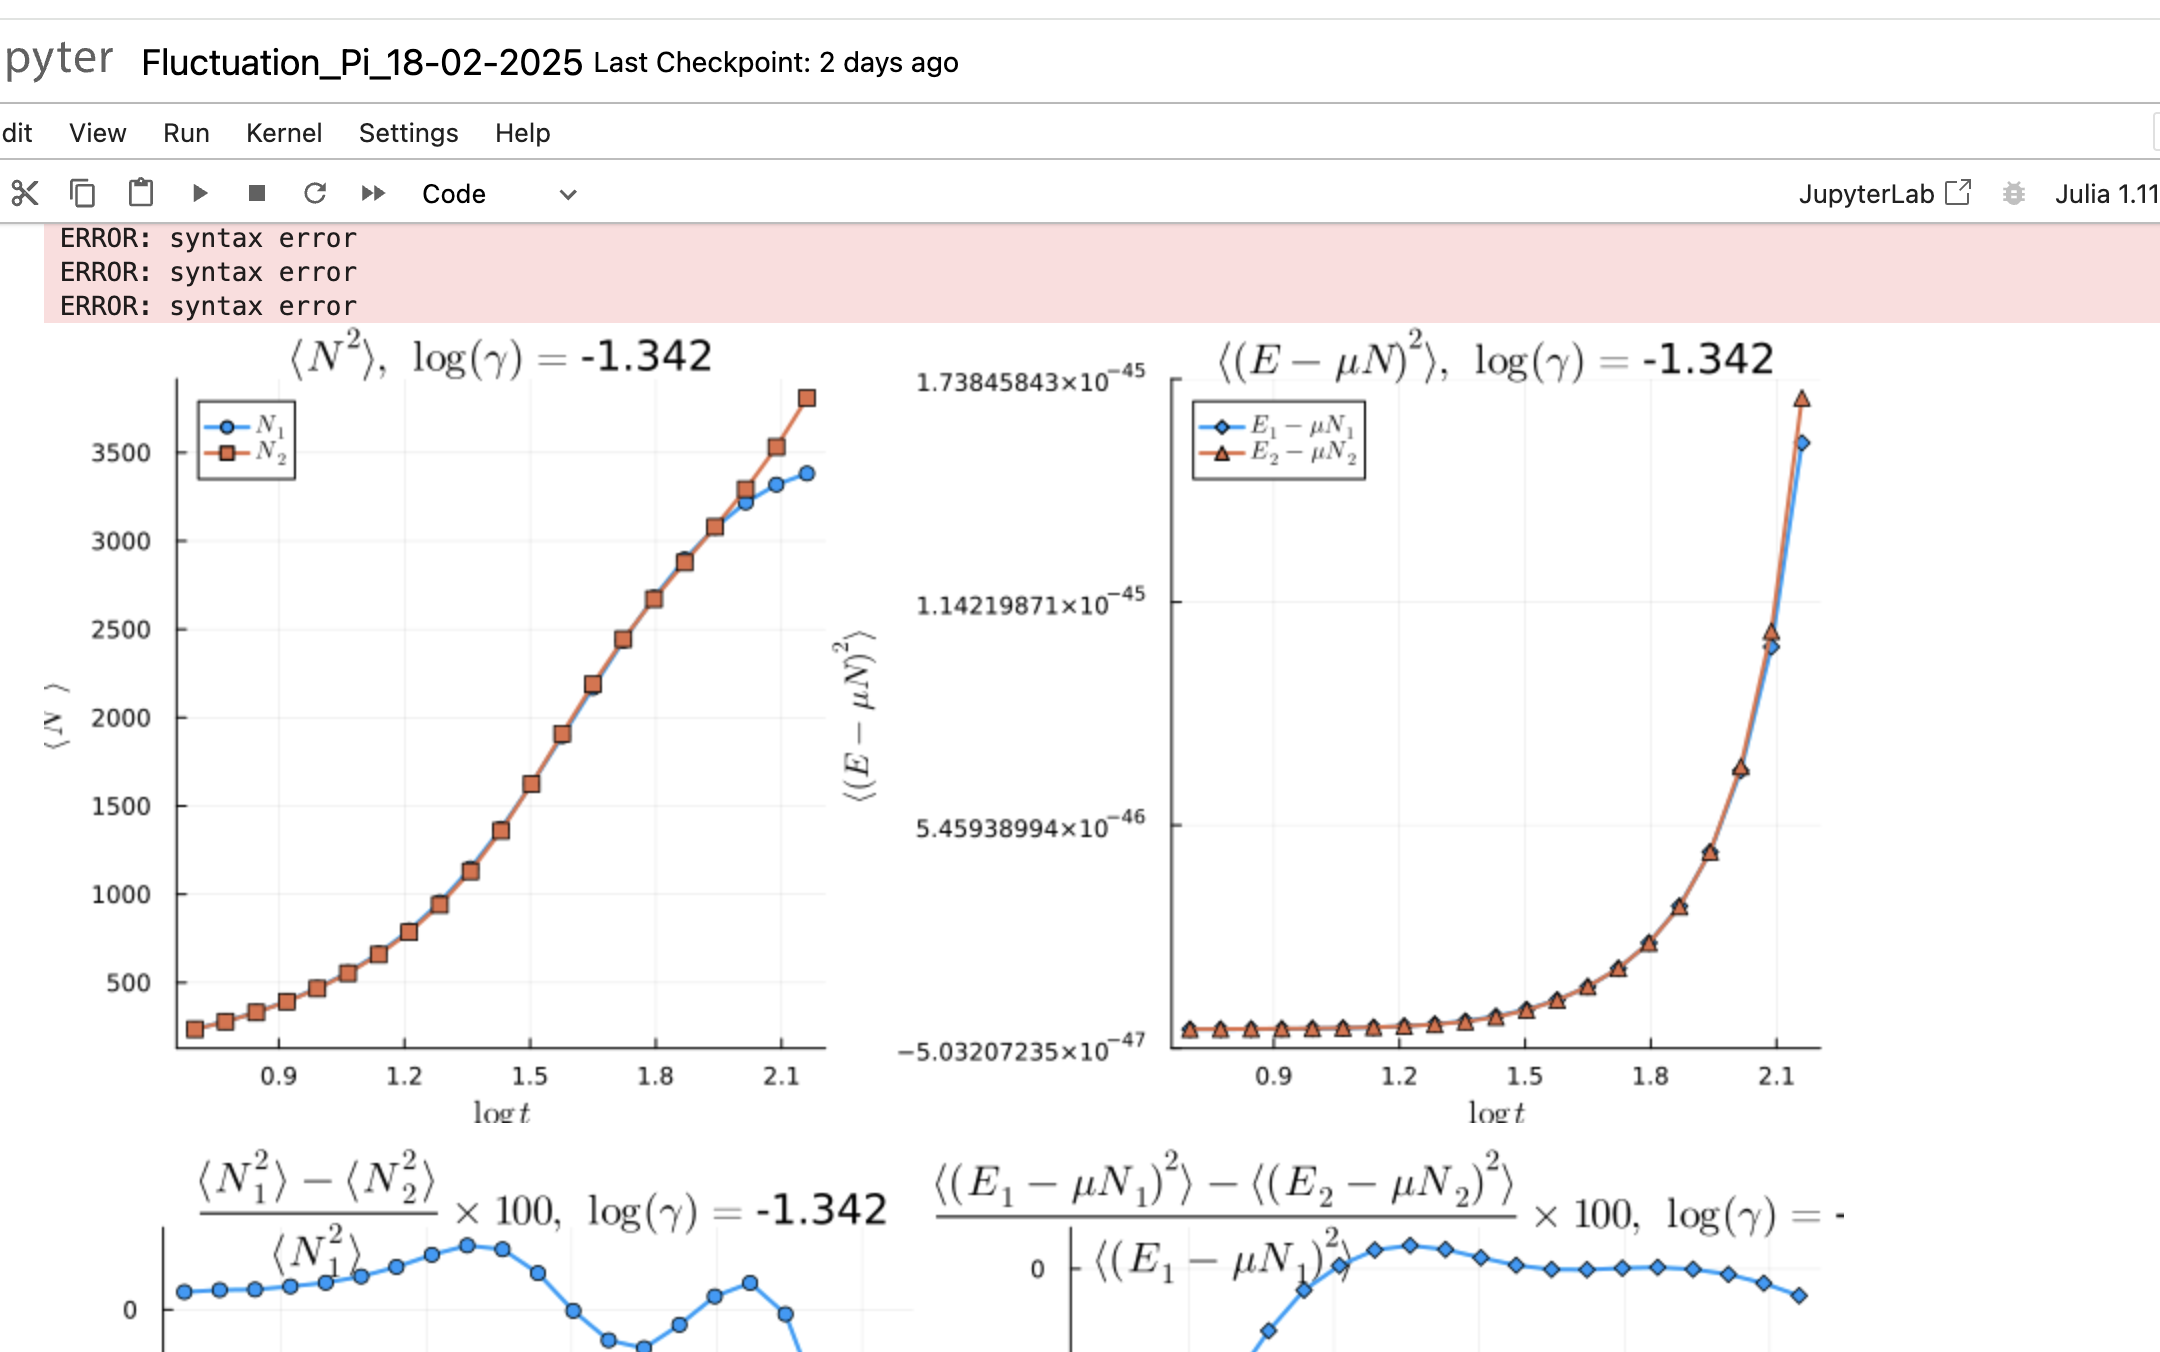
\includegraphics[width=1\textwidth]{Figures/test}

%\begin{aff}
%Donc une a l'ordre un en $\delta \theta (\operator{A}^{(0)})^{-1} %\operator{V}$ 

%\begin{eqnarray*}
%	\langle \delta \Pi ( \theta) \delta \Pi ( \theta') \rangle & = &  ( (\Pi^c_s - \Pi^c)\Pi^c/\Pi^c_s ) ( \theta ) \delta_{\theta, \theta'}/\delta \theta + \mathscr{F}(\theta , \theta' ) ,	
%\end{eqnarray*}

%avec 

%\begin{eqnarray*}
%	\mathscr{F}(\theta , \theta' ) & = & \left [ (\Pi^c_s - \Pi^c )( \theta)  +  (\Pi^c_s - \Pi^c ) ( \theta' )\right ] \frac{\Pi^c}{\Pi^c_s}(\theta)\frac{\Pi^c}{\Pi^c_s}(\theta') \frac{ \Delta( \theta'- \theta )}{ 2 \pi }\\
%	&&  - \left [ (\Pi^c_s - \Pi^c )( \theta)   (\Pi^c_s - \Pi^c ) ( \theta' )\right ] \frac{\Pi^c}{\Pi^c_s}(\theta)\frac{\Pi^c}{\Pi^c_s}(\theta')\int d\theta'' \left (   \frac{ \Pi^c/\Pi^c_s}{\Pi^c_s - \Pi^c} \right )(\theta'') \frac{\Delta(\theta''- \theta)}{2 \pi}\frac{\Delta(\theta''- \theta')}{2 \pi}  	
%\end{eqnarray*}
%\end{aff}



 









\subsection{États du vide et pseudovacuum}
%Dans ce chapitre, nous nous intéressons aux fluctuations de la distribution de rapidité \( \delta \rho \) autour d'une distribution de référence \( \rho^c \), qui maximise la contribution à la fonction de partition des états, exprimée comme une fonctionnelle de la distribution \( \rho \) : 

La fonction de partition des états, s'exprime comme une fonctionnelle de la distribution \( \rho \) : 

\begin{eqnarray*}
	\Xi & = & \sum_\rho \exp \left( -\mathcal{A}(\rho) \right).
\end{eqnarray*}  

Dans la section {\em \bf Entropie de Yang-Yang} (\ref{??}), l'action \( \mathcal{A}(\rho) \) s'écrit sous la forme :  

\begin{eqnarray*}
	\mathcal{A}(\rho) & \doteq & - L\mathcal{S}_{YY}(\rho) + L\int f(\theta) \rho (\theta) \, d\theta,		
\end{eqnarray*}  

où \( \mathcal{S}_{YY} \) est la fonctionnelle d'entropie de Yang-Yang, définie dans (\ref{??}), et \( f \) est la fonction paramétrant les charges, introduite dans (\ref{??}).  

Dans cette même section {\em \bf Entropie de Yang-Yang} (\ref{??}), nous avons établi un lien entre \( f \) et distribution de référence \( \rho^c \), qui maximise la contribution à la fonction de partition des états .\\

On veux tester si nos experience est décrit pas un GGE. Pour cela nous nous intéressons aux fluctuations de la distribution de rapidité \( \delta \rho \) autour \( \rho^c \).

%Nous poursuivons à présent avec cette définition de l'action de classe $\mathcal{C}^2$ et admetant une distribution critique $\rho^c$ tel que sa différentielle en ce point critique soit nulle $d\mathcal{A}_{\rho^c} = 0 $ (\ref{??}) de sorte que d'aprés la formule de Taylor-Youg %afin de déterminer les fluctuations autour de \( \Pi^c \). Pour cela, nous réécrivons l'action sous la forme :  

Nous poursuivons à présent avec cette définition de l'action de classe $\mathcal{C}^2$ et admetant une distribution critique $\rho^c$ tel que sa différentielle en ce point critique soit nulle $d\mathcal{A}_{\rho^c} = 0 $ (\ref{??}) de sorte que d'aprés la formule de Taylor-Youg %afin de déterminer les fluctuations autour de \( \Pi^c \). Pour cela, nous réécrivons l'action sous la forme :  

\begin{eqnarray*}  
	\mathcal{A}(\rho^c + \delta \rho) & \underset{ \delta \rho \to 0 }{=} & \mathcal{A}(\rho^c)  + \frac{1}{2} \left. \frac{\delta^2 \mathcal{A}}{\delta \rho^2} \right|_{\rho^c} (\delta \rho) + \mathcal{O}((\delta \rho)^3),  
\end{eqnarray*}  

une expression quadratique pour l'action à l'ordre dominant en \( \delta \Pi \) avec $\left. \frac{\delta^2 \mathcal{A}}{\delta \rho^2} \right|_{\rho^c}$ la forme quadratique définie positive (Fig (\ref{fig.fluctu.A})).

\begin{figure}[H]
	\centering 
	\begin{tikzpicture}
		\begin{scope}[shift={(0,0)}]
			\begin{scope}[transform canvas={scale=0.6}]
				\input{Figures/Fonc_A_code}	
			
			\end{scope}
			
			\draw[color = red , scale = 0.5 , draw = none  ] (-2 , -1) rectangle (5, 6) ; 	
		\end{scope}
		
		\begin{scope}[shift={(19,-1)}]
			\begin{scope}[transform canvas={scale=0.6}]
				\input{Figures/Occupation_theta_code}	
			
			\end{scope}
			\begin{scope}[scale=1]
				\draw[color = red , scale = 1 , draw = none  ] (-1 , -1) rectangle (5, 5) ; 
			\end{scope}	
		\end{scope}

		
				
			
	\end{tikzpicture}	
	\captionsetup{skip=10pt} % Ajoute de l’espace après la légende
	\label{fig.fluctu.A}
\end{figure}


On discrétise l'axe des rapidités en  petite cellule de rapidité $[\theta, \theta+\delta\theta]$, qui contient $L\rho(\theta) \delta \theta$ rapidités. 
	



Avec ces petites tranches, la forme quadratique s’écrit :

\begin{eqnarray*}
    \left. \frac{\delta^2 \mathcal{A}}{{\delta \rho}^2} \right|_{\rho^c}(\delta \rho ) &=&  \sum_{a,b \mid \text{tranche}}  
    \delta \rho(\theta_a)  \frac{\partial^2 \mathcal{A}}{\partial \delta \rho(\theta_a) \partial \delta \rho(\theta_b) } (\rho^c)  \delta \rho(\theta_b).
\end{eqnarray*}
Les fluctuations s’écrivent donc :

\begin{eqnarray*}
    \langle \delta \rho ( \theta) \delta \rho ( \theta') \rangle &=&  
    \frac{ \int d\delta \rho \, \delta \rho(\theta) \delta \rho ( \theta') 
    \exp \left( - \frac{1}{2} \sum_{a,b \mid \text{tranche}}  
    \delta \rho(\theta_a) \frac{\partial^2 \mathcal{A}}{\partial \delta \rho(\theta_a) \partial \delta \rho(\theta_b) } (\rho^c)  \delta \rho(\theta_b) \right) }
    { \int d\delta \Pi  
    \exp \left( - \frac{1}{2} \sum_{a,b \mid \text{tranche}}  
    \delta \rho(\theta_a) \frac{\partial^2 \mathcal{A}}{\partial \delta \rho(\theta_a) \partial \delta \rho(\theta_b) } (\rho^c)  \delta \rho(\theta_b) \right) } \\
    &=& \left( \mathbf{A}^{-1} \right)_{\theta , \theta'}
\end{eqnarray*}


\begin{aff}

\begin{eqnarray*}
	\langle \delta \rho ( \theta) \delta \rho ( \theta') \rangle &=& 	\left( \mathbf{A}^{-1} \right)_{\theta , \theta'}
\end{eqnarray*}

	
avec la  {\em matrice hessienne} $\mathbf{A}_{\theta , \theta'} \equiv \frac{\partial^2 \mathcal{A}}{\partial \delta \rho(\theta) \partial \delta \rho(\theta') }(\rho^c)$, au point critique/ qui maximise la probabilité  $\rho^c=\rho^c_s \nu^c $, s'écrit

\begin{eqnarray*}
	\operator{A} & = & \operator{A}^{(0)} + \delta \theta \operator{V}
\end{eqnarray*}

avec 

\begin{eqnarray*}
	A^{(0)}_{\theta , \theta'}  & = &  L\delta \theta \left ( \frac{ 1}{\rho^c_s ( 1  - \nu^c ) \nu^c } \right )(\theta)    \delta({\theta - \theta '})	,\\
	V_{\theta , \theta'}  &= & L \delta \theta \left \{ - \left [ \left ( \frac{1}{\rho^c_s( 1 - \nu^c) } \right ) ( \theta)  +  \left ( \frac{1}{\rho^c_s( 1 - \nu^c) } \right ) ( \theta' )\right ] \frac{ \Delta( \theta'- \theta )}{ 2 \pi } + \int d\theta''  \left ( \frac{\nu^c}{\rho^c_s( 1 - \nu^c) } \right )(\theta'') \frac{\Delta(\theta''- \theta)}{2 \pi}\frac{\Delta(\theta''- \theta')}{2 \pi}   \right \} 	
\end{eqnarray*}

\end{aff}

\subsection{Testes}

\begin{eqnarray*}
	\Delta_{\operator{\mathcal{N}}}^2  & = &  \frac{1}{\beta} \left . \frac{\partial \langle \operator{\mathcal{N}} \rangle}{\partial \mu} \right )_T \\
	\Delta_{\operator{\mathcal{E}}-\mu \operator{\mathcal{N}}}^2  & = &  - \left . \frac{\partial \langle \operator{\mathcal{E}}-\mu \operator{\mathcal{N}} \rangle}{\partial \beta} \right )_\mu 
\end{eqnarray*}

et 

\begin{eqnarray*}
	\Delta_{\operator{\mathcal{N}}}^2  &= & L^2 \int d\theta_a \int d \theta_b \, \langle \delta \rho(\theta_a) \delta \rho(\theta_b) \rangle \\
	\Delta_{\operator{\mathcal{E}}-\mu \operator{\mathcal{N}}}^2  & = & L^2 \int d\theta_a \int d \theta_b \, \left ( - \mu + \frac{1}2 m \theta_a^2  \right  )\left ( - \mu + \frac{1}2 m \theta_b^2  \right  )  \langle \delta \rho(\theta_a) \delta \rho(\theta_b) \rangle
\end{eqnarray*}

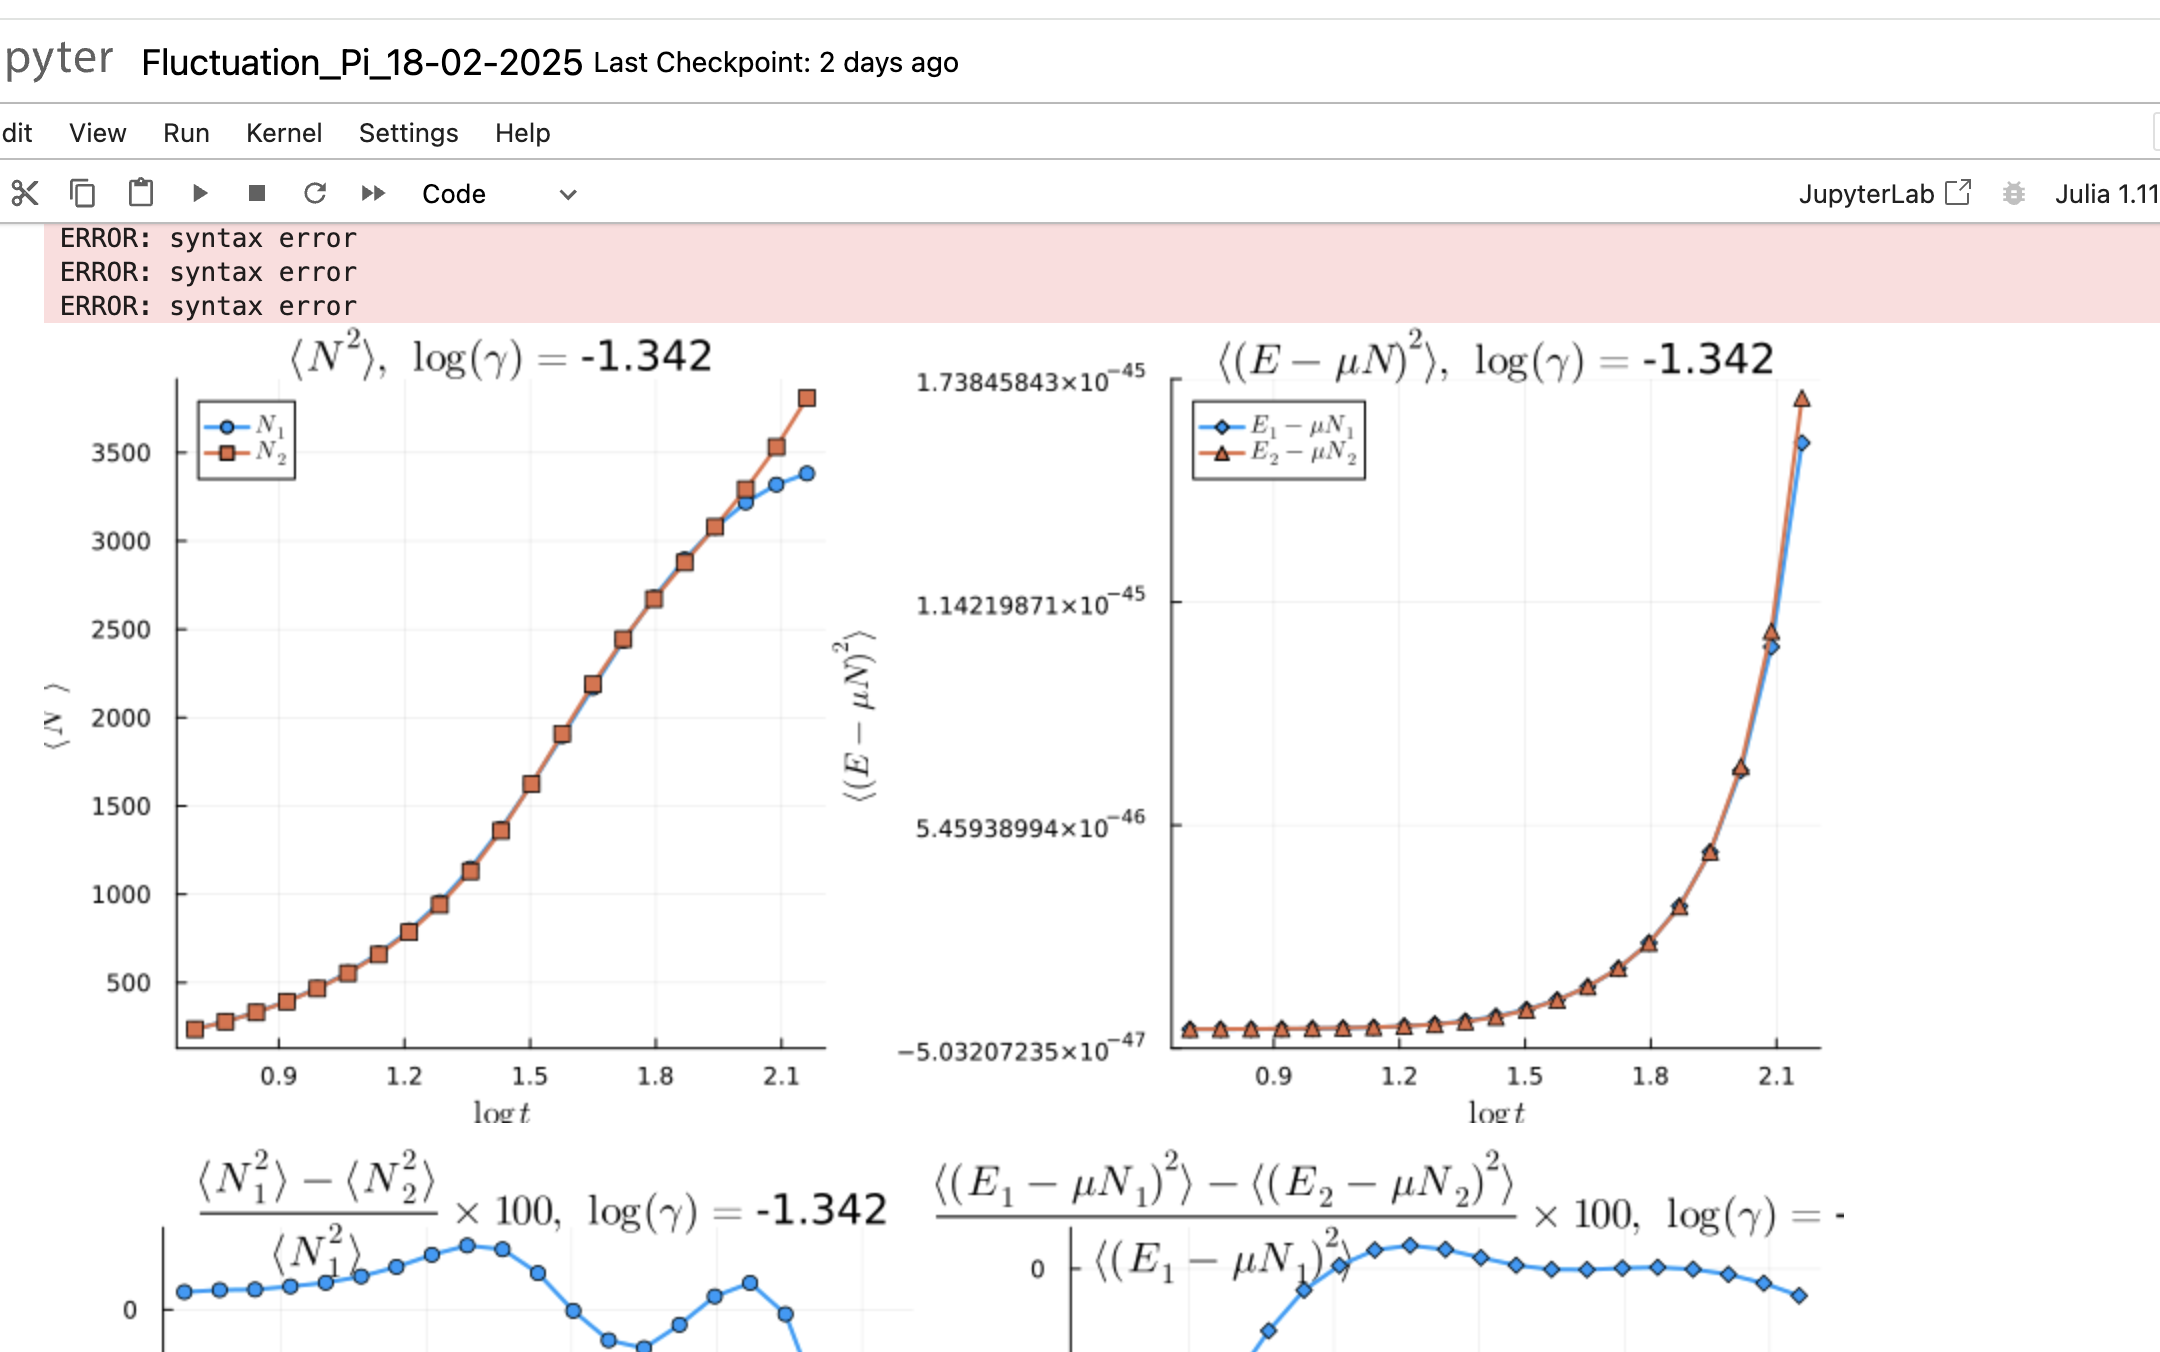
\includegraphics[width=1\textwidth]{Figures/test}

%\begin{aff}
%Donc une a l'ordre un en $\delta \theta (\operator{A}^{(0)})^{-1} %\operator{V}$ 

%\begin{eqnarray*}
%	\langle \delta \Pi ( \theta) \delta \Pi ( \theta') \rangle & = &  ( (\Pi^c_s - \Pi^c)\Pi^c/\Pi^c_s ) ( \theta ) \delta_{\theta, \theta'}/\delta \theta + \mathscr{F}(\theta , \theta' ) ,	
%\end{eqnarray*}

%avec 

%\begin{eqnarray*}
%	\mathscr{F}(\theta , \theta' ) & = & \left [ (\Pi^c_s - \Pi^c )( \theta)  +  (\Pi^c_s - \Pi^c ) ( \theta' )\right ] \frac{\Pi^c}{\Pi^c_s}(\theta)\frac{\Pi^c}{\Pi^c_s}(\theta') \frac{ \Delta( \theta'- \theta )}{ 2 \pi }\\
%	&&  - \left [ (\Pi^c_s - \Pi^c )( \theta)   (\Pi^c_s - \Pi^c ) ( \theta' )\right ] \frac{\Pi^c}{\Pi^c_s}(\theta)\frac{\Pi^c}{\Pi^c_s}(\theta')\int d\theta'' \left (   \frac{ \Pi^c/\Pi^c_s}{\Pi^c_s - \Pi^c} \right )(\theta'') \frac{\Delta(\theta''- \theta)}{2 \pi}\frac{\Delta(\theta''- \theta')}{2 \pi}  	
%\end{eqnarray*}
%\end{aff}



 










\subsection{Opérateurs conservés (intégrales du mouvement)}
%Dans ce chapitre, nous nous intéressons aux fluctuations de la distribution de rapidité \( \delta \rho \) autour d'une distribution de référence \( \rho^c \), qui maximise la contribution à la fonction de partition des états, exprimée comme une fonctionnelle de la distribution \( \rho \) : 

La fonction de partition des états, s'exprime comme une fonctionnelle de la distribution \( \rho \) : 

\begin{eqnarray*}
	\Xi & = & \sum_\rho \exp \left( -\mathcal{A}(\rho) \right).
\end{eqnarray*}  

Dans la section {\em \bf Entropie de Yang-Yang} (\ref{??}), l'action \( \mathcal{A}(\rho) \) s'écrit sous la forme :  

\begin{eqnarray*}
	\mathcal{A}(\rho) & \doteq & - L\mathcal{S}_{YY}(\rho) + L\int f(\theta) \rho (\theta) \, d\theta,		
\end{eqnarray*}  

où \( \mathcal{S}_{YY} \) est la fonctionnelle d'entropie de Yang-Yang, définie dans (\ref{??}), et \( f \) est la fonction paramétrant les charges, introduite dans (\ref{??}).  

Dans cette même section {\em \bf Entropie de Yang-Yang} (\ref{??}), nous avons établi un lien entre \( f \) et distribution de référence \( \rho^c \), qui maximise la contribution à la fonction de partition des états .\\

On veux tester si nos experience est décrit pas un GGE. Pour cela nous nous intéressons aux fluctuations de la distribution de rapidité \( \delta \rho \) autour \( \rho^c \).

%Nous poursuivons à présent avec cette définition de l'action de classe $\mathcal{C}^2$ et admetant une distribution critique $\rho^c$ tel que sa différentielle en ce point critique soit nulle $d\mathcal{A}_{\rho^c} = 0 $ (\ref{??}) de sorte que d'aprés la formule de Taylor-Youg %afin de déterminer les fluctuations autour de \( \Pi^c \). Pour cela, nous réécrivons l'action sous la forme :  

Nous poursuivons à présent avec cette définition de l'action de classe $\mathcal{C}^2$ et admetant une distribution critique $\rho^c$ tel que sa différentielle en ce point critique soit nulle $d\mathcal{A}_{\rho^c} = 0 $ (\ref{??}) de sorte que d'aprés la formule de Taylor-Youg %afin de déterminer les fluctuations autour de \( \Pi^c \). Pour cela, nous réécrivons l'action sous la forme :  

\begin{eqnarray*}  
	\mathcal{A}(\rho^c + \delta \rho) & \underset{ \delta \rho \to 0 }{=} & \mathcal{A}(\rho^c)  + \frac{1}{2} \left. \frac{\delta^2 \mathcal{A}}{\delta \rho^2} \right|_{\rho^c} (\delta \rho) + \mathcal{O}((\delta \rho)^3),  
\end{eqnarray*}  

une expression quadratique pour l'action à l'ordre dominant en \( \delta \Pi \) avec $\left. \frac{\delta^2 \mathcal{A}}{\delta \rho^2} \right|_{\rho^c}$ la forme quadratique définie positive (Fig (\ref{fig.fluctu.A})).

\begin{figure}[H]
	\centering 
	\begin{tikzpicture}
		\begin{scope}[shift={(0,0)}]
			\begin{scope}[transform canvas={scale=0.6}]
				\input{Figures/Fonc_A_code}	
			
			\end{scope}
			
			\draw[color = red , scale = 0.5 , draw = none  ] (-2 , -1) rectangle (5, 6) ; 	
		\end{scope}
		
		\begin{scope}[shift={(19,-1)}]
			\begin{scope}[transform canvas={scale=0.6}]
				\input{Figures/Occupation_theta_code}	
			
			\end{scope}
			\begin{scope}[scale=1]
				\draw[color = red , scale = 1 , draw = none  ] (-1 , -1) rectangle (5, 5) ; 
			\end{scope}	
		\end{scope}

		
				
			
	\end{tikzpicture}	
	\captionsetup{skip=10pt} % Ajoute de l’espace après la légende
	\label{fig.fluctu.A}
\end{figure}


On discrétise l'axe des rapidités en  petite cellule de rapidité $[\theta, \theta+\delta\theta]$, qui contient $L\rho(\theta) \delta \theta$ rapidités. 
	



Avec ces petites tranches, la forme quadratique s’écrit :

\begin{eqnarray*}
    \left. \frac{\delta^2 \mathcal{A}}{{\delta \rho}^2} \right|_{\rho^c}(\delta \rho ) &=&  \sum_{a,b \mid \text{tranche}}  
    \delta \rho(\theta_a)  \frac{\partial^2 \mathcal{A}}{\partial \delta \rho(\theta_a) \partial \delta \rho(\theta_b) } (\rho^c)  \delta \rho(\theta_b).
\end{eqnarray*}
Les fluctuations s’écrivent donc :

\begin{eqnarray*}
    \langle \delta \rho ( \theta) \delta \rho ( \theta') \rangle &=&  
    \frac{ \int d\delta \rho \, \delta \rho(\theta) \delta \rho ( \theta') 
    \exp \left( - \frac{1}{2} \sum_{a,b \mid \text{tranche}}  
    \delta \rho(\theta_a) \frac{\partial^2 \mathcal{A}}{\partial \delta \rho(\theta_a) \partial \delta \rho(\theta_b) } (\rho^c)  \delta \rho(\theta_b) \right) }
    { \int d\delta \Pi  
    \exp \left( - \frac{1}{2} \sum_{a,b \mid \text{tranche}}  
    \delta \rho(\theta_a) \frac{\partial^2 \mathcal{A}}{\partial \delta \rho(\theta_a) \partial \delta \rho(\theta_b) } (\rho^c)  \delta \rho(\theta_b) \right) } \\
    &=& \left( \mathbf{A}^{-1} \right)_{\theta , \theta'}
\end{eqnarray*}


\begin{aff}

\begin{eqnarray*}
	\langle \delta \rho ( \theta) \delta \rho ( \theta') \rangle &=& 	\left( \mathbf{A}^{-1} \right)_{\theta , \theta'}
\end{eqnarray*}

	
avec la  {\em matrice hessienne} $\mathbf{A}_{\theta , \theta'} \equiv \frac{\partial^2 \mathcal{A}}{\partial \delta \rho(\theta) \partial \delta \rho(\theta') }(\rho^c)$, au point critique/ qui maximise la probabilité  $\rho^c=\rho^c_s \nu^c $, s'écrit

\begin{eqnarray*}
	\operator{A} & = & \operator{A}^{(0)} + \delta \theta \operator{V}
\end{eqnarray*}

avec 

\begin{eqnarray*}
	A^{(0)}_{\theta , \theta'}  & = &  L\delta \theta \left ( \frac{ 1}{\rho^c_s ( 1  - \nu^c ) \nu^c } \right )(\theta)    \delta({\theta - \theta '})	,\\
	V_{\theta , \theta'}  &= & L \delta \theta \left \{ - \left [ \left ( \frac{1}{\rho^c_s( 1 - \nu^c) } \right ) ( \theta)  +  \left ( \frac{1}{\rho^c_s( 1 - \nu^c) } \right ) ( \theta' )\right ] \frac{ \Delta( \theta'- \theta )}{ 2 \pi } + \int d\theta''  \left ( \frac{\nu^c}{\rho^c_s( 1 - \nu^c) } \right )(\theta'') \frac{\Delta(\theta''- \theta)}{2 \pi}\frac{\Delta(\theta''- \theta')}{2 \pi}   \right \} 	
\end{eqnarray*}

\end{aff}

\subsection{Testes}

\begin{eqnarray*}
	\Delta_{\operator{\mathcal{N}}}^2  & = &  \frac{1}{\beta} \left . \frac{\partial \langle \operator{\mathcal{N}} \rangle}{\partial \mu} \right )_T \\
	\Delta_{\operator{\mathcal{E}}-\mu \operator{\mathcal{N}}}^2  & = &  - \left . \frac{\partial \langle \operator{\mathcal{E}}-\mu \operator{\mathcal{N}} \rangle}{\partial \beta} \right )_\mu 
\end{eqnarray*}

et 

\begin{eqnarray*}
	\Delta_{\operator{\mathcal{N}}}^2  &= & L^2 \int d\theta_a \int d \theta_b \, \langle \delta \rho(\theta_a) \delta \rho(\theta_b) \rangle \\
	\Delta_{\operator{\mathcal{E}}-\mu \operator{\mathcal{N}}}^2  & = & L^2 \int d\theta_a \int d \theta_b \, \left ( - \mu + \frac{1}2 m \theta_a^2  \right  )\left ( - \mu + \frac{1}2 m \theta_b^2  \right  )  \langle \delta \rho(\theta_a) \delta \rho(\theta_b) \rangle
\end{eqnarray*}

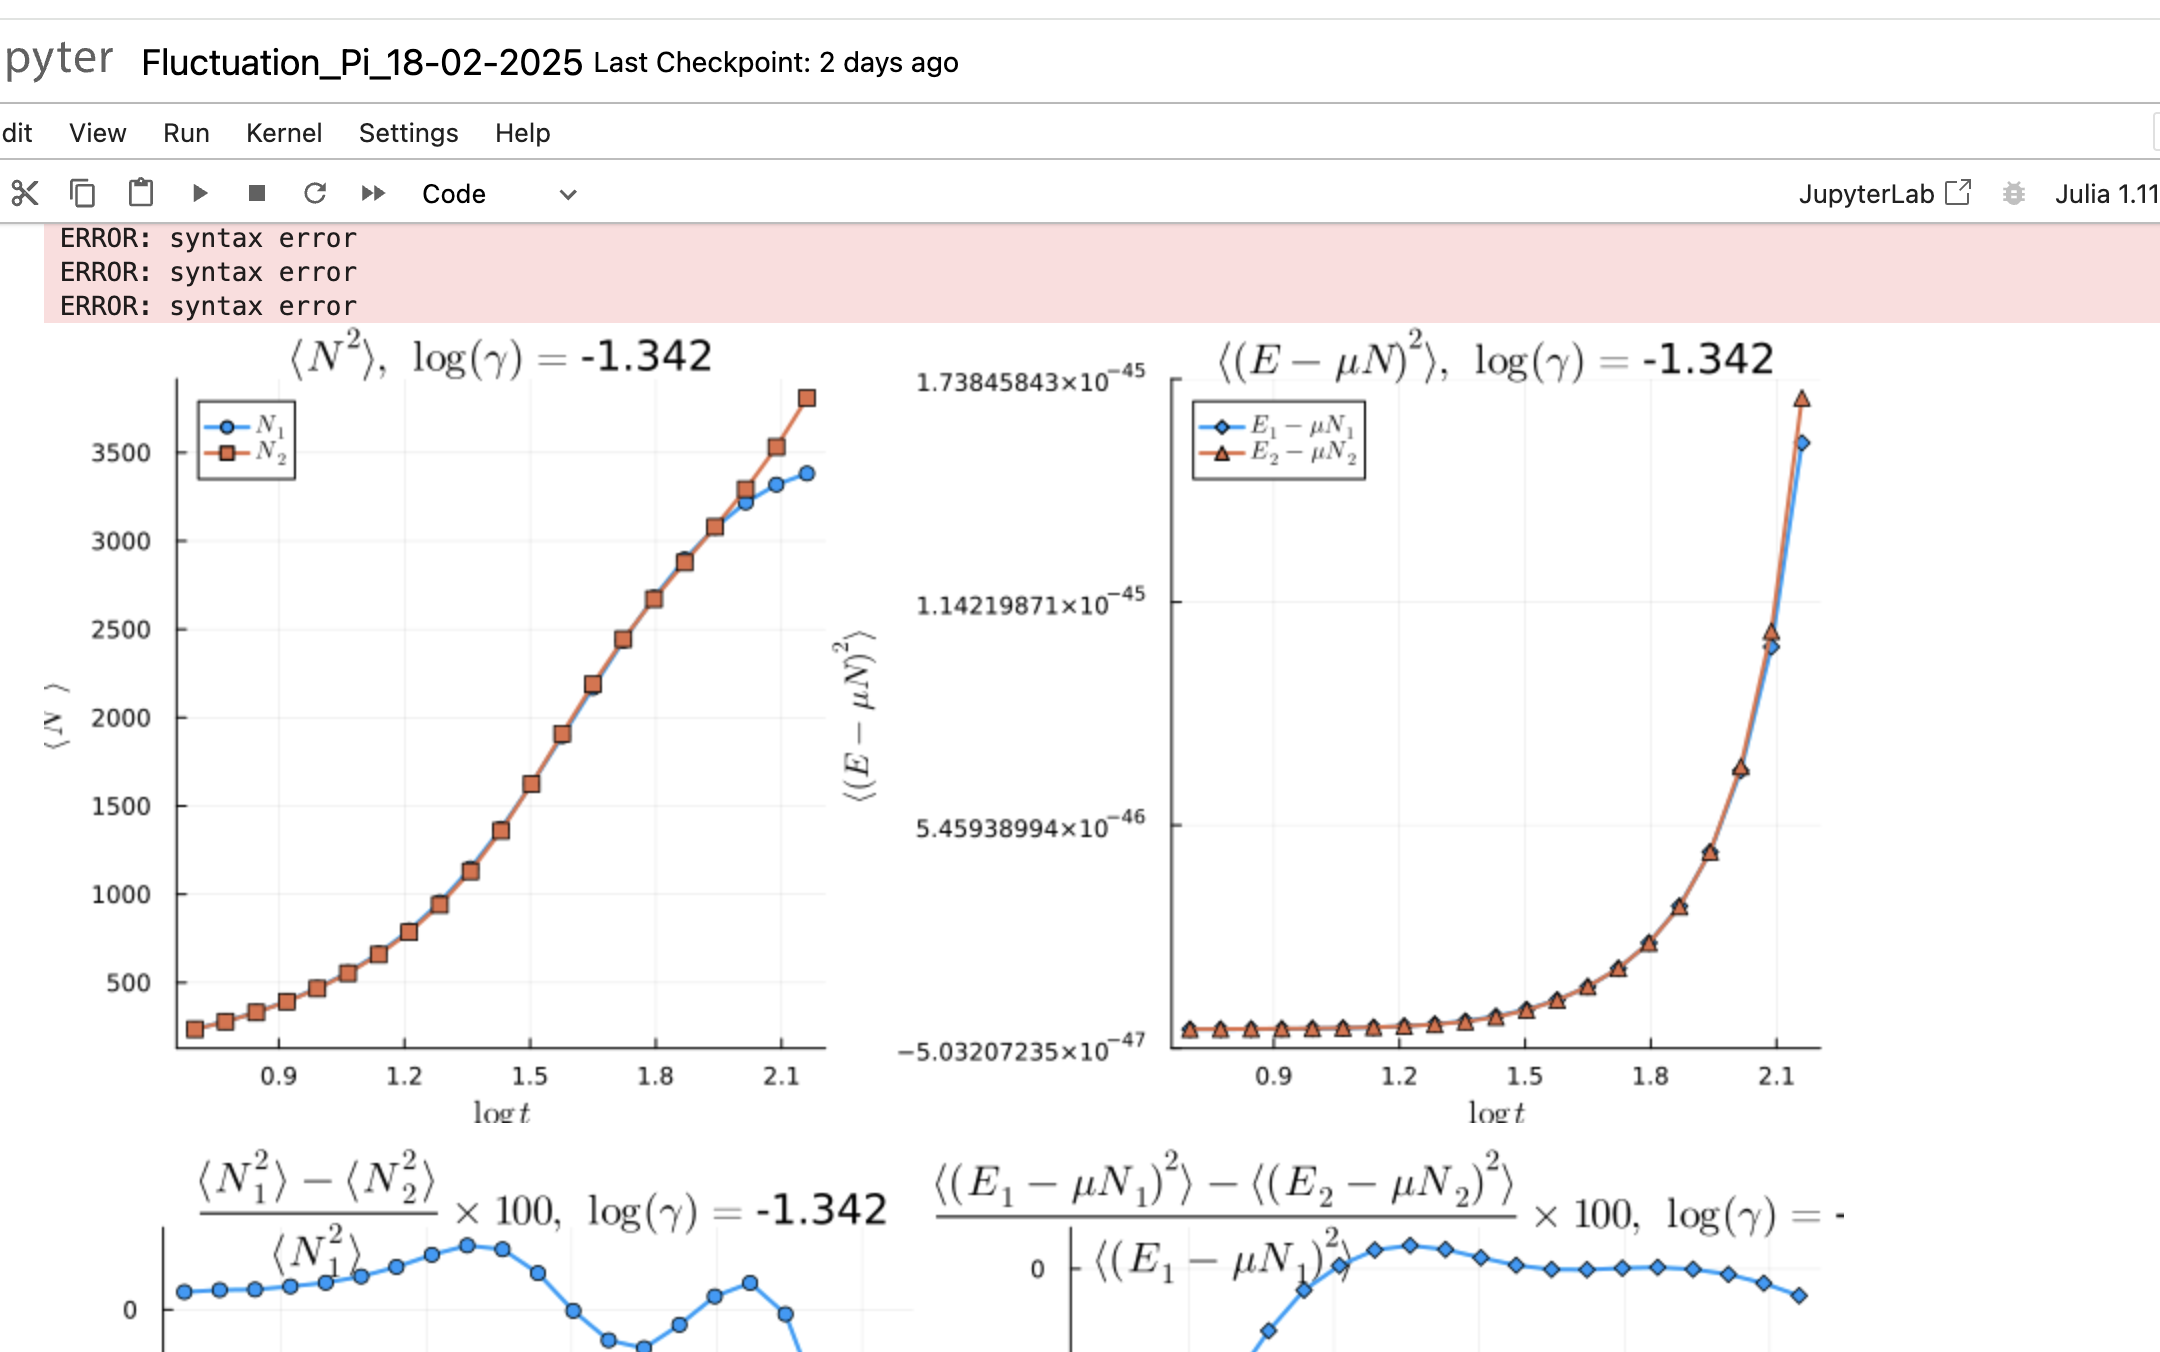
\includegraphics[width=1\textwidth]{Figures/test}

%\begin{aff}
%Donc une a l'ordre un en $\delta \theta (\operator{A}^{(0)})^{-1} %\operator{V}$ 

%\begin{eqnarray*}
%	\langle \delta \Pi ( \theta) \delta \Pi ( \theta') \rangle & = &  ( (\Pi^c_s - \Pi^c)\Pi^c/\Pi^c_s ) ( \theta ) \delta_{\theta, \theta'}/\delta \theta + \mathscr{F}(\theta , \theta' ) ,	
%\end{eqnarray*}

%avec 

%\begin{eqnarray*}
%	\mathscr{F}(\theta , \theta' ) & = & \left [ (\Pi^c_s - \Pi^c )( \theta)  +  (\Pi^c_s - \Pi^c ) ( \theta' )\right ] \frac{\Pi^c}{\Pi^c_s}(\theta)\frac{\Pi^c}{\Pi^c_s}(\theta') \frac{ \Delta( \theta'- \theta )}{ 2 \pi }\\
%	&&  - \left [ (\Pi^c_s - \Pi^c )( \theta)   (\Pi^c_s - \Pi^c ) ( \theta' )\right ] \frac{\Pi^c}{\Pi^c_s}(\theta)\frac{\Pi^c}{\Pi^c_s}(\theta')\int d\theta'' \left (   \frac{ \Pi^c/\Pi^c_s}{\Pi^c_s - \Pi^c} \right )(\theta'') \frac{\Delta(\theta''- \theta)}{2 \pi}\frac{\Delta(\theta''- \theta')}{2 \pi}  	
%\end{eqnarray*}
%\end{aff}



 








 
\subsection{Fonction d’onde $\chi_N$ et Hamiltonien et moment à N corps}
%Dans ce chapitre, nous nous intéressons aux fluctuations de la distribution de rapidité \( \delta \rho \) autour d'une distribution de référence \( \rho^c \), qui maximise la contribution à la fonction de partition des états, exprimée comme une fonctionnelle de la distribution \( \rho \) : 

La fonction de partition des états, s'exprime comme une fonctionnelle de la distribution \( \rho \) : 

\begin{eqnarray*}
	\Xi & = & \sum_\rho \exp \left( -\mathcal{A}(\rho) \right).
\end{eqnarray*}  

Dans la section {\em \bf Entropie de Yang-Yang} (\ref{??}), l'action \( \mathcal{A}(\rho) \) s'écrit sous la forme :  

\begin{eqnarray*}
	\mathcal{A}(\rho) & \doteq & - L\mathcal{S}_{YY}(\rho) + L\int f(\theta) \rho (\theta) \, d\theta,		
\end{eqnarray*}  

où \( \mathcal{S}_{YY} \) est la fonctionnelle d'entropie de Yang-Yang, définie dans (\ref{??}), et \( f \) est la fonction paramétrant les charges, introduite dans (\ref{??}).  

Dans cette même section {\em \bf Entropie de Yang-Yang} (\ref{??}), nous avons établi un lien entre \( f \) et distribution de référence \( \rho^c \), qui maximise la contribution à la fonction de partition des états .\\

On veux tester si nos experience est décrit pas un GGE. Pour cela nous nous intéressons aux fluctuations de la distribution de rapidité \( \delta \rho \) autour \( \rho^c \).

%Nous poursuivons à présent avec cette définition de l'action de classe $\mathcal{C}^2$ et admetant une distribution critique $\rho^c$ tel que sa différentielle en ce point critique soit nulle $d\mathcal{A}_{\rho^c} = 0 $ (\ref{??}) de sorte que d'aprés la formule de Taylor-Youg %afin de déterminer les fluctuations autour de \( \Pi^c \). Pour cela, nous réécrivons l'action sous la forme :  

Nous poursuivons à présent avec cette définition de l'action de classe $\mathcal{C}^2$ et admetant une distribution critique $\rho^c$ tel que sa différentielle en ce point critique soit nulle $d\mathcal{A}_{\rho^c} = 0 $ (\ref{??}) de sorte que d'aprés la formule de Taylor-Youg %afin de déterminer les fluctuations autour de \( \Pi^c \). Pour cela, nous réécrivons l'action sous la forme :  

\begin{eqnarray*}  
	\mathcal{A}(\rho^c + \delta \rho) & \underset{ \delta \rho \to 0 }{=} & \mathcal{A}(\rho^c)  + \frac{1}{2} \left. \frac{\delta^2 \mathcal{A}}{\delta \rho^2} \right|_{\rho^c} (\delta \rho) + \mathcal{O}((\delta \rho)^3),  
\end{eqnarray*}  

une expression quadratique pour l'action à l'ordre dominant en \( \delta \Pi \) avec $\left. \frac{\delta^2 \mathcal{A}}{\delta \rho^2} \right|_{\rho^c}$ la forme quadratique définie positive (Fig (\ref{fig.fluctu.A})).

\begin{figure}[H]
	\centering 
	\begin{tikzpicture}
		\begin{scope}[shift={(0,0)}]
			\begin{scope}[transform canvas={scale=0.6}]
				\input{Figures/Fonc_A_code}	
			
			\end{scope}
			
			\draw[color = red , scale = 0.5 , draw = none  ] (-2 , -1) rectangle (5, 6) ; 	
		\end{scope}
		
		\begin{scope}[shift={(19,-1)}]
			\begin{scope}[transform canvas={scale=0.6}]
				\input{Figures/Occupation_theta_code}	
			
			\end{scope}
			\begin{scope}[scale=1]
				\draw[color = red , scale = 1 , draw = none  ] (-1 , -1) rectangle (5, 5) ; 
			\end{scope}	
		\end{scope}

		
				
			
	\end{tikzpicture}	
	\captionsetup{skip=10pt} % Ajoute de l’espace après la légende
	\label{fig.fluctu.A}
\end{figure}


On discrétise l'axe des rapidités en  petite cellule de rapidité $[\theta, \theta+\delta\theta]$, qui contient $L\rho(\theta) \delta \theta$ rapidités. 
	



Avec ces petites tranches, la forme quadratique s’écrit :

\begin{eqnarray*}
    \left. \frac{\delta^2 \mathcal{A}}{{\delta \rho}^2} \right|_{\rho^c}(\delta \rho ) &=&  \sum_{a,b \mid \text{tranche}}  
    \delta \rho(\theta_a)  \frac{\partial^2 \mathcal{A}}{\partial \delta \rho(\theta_a) \partial \delta \rho(\theta_b) } (\rho^c)  \delta \rho(\theta_b).
\end{eqnarray*}
Les fluctuations s’écrivent donc :

\begin{eqnarray*}
    \langle \delta \rho ( \theta) \delta \rho ( \theta') \rangle &=&  
    \frac{ \int d\delta \rho \, \delta \rho(\theta) \delta \rho ( \theta') 
    \exp \left( - \frac{1}{2} \sum_{a,b \mid \text{tranche}}  
    \delta \rho(\theta_a) \frac{\partial^2 \mathcal{A}}{\partial \delta \rho(\theta_a) \partial \delta \rho(\theta_b) } (\rho^c)  \delta \rho(\theta_b) \right) }
    { \int d\delta \Pi  
    \exp \left( - \frac{1}{2} \sum_{a,b \mid \text{tranche}}  
    \delta \rho(\theta_a) \frac{\partial^2 \mathcal{A}}{\partial \delta \rho(\theta_a) \partial \delta \rho(\theta_b) } (\rho^c)  \delta \rho(\theta_b) \right) } \\
    &=& \left( \mathbf{A}^{-1} \right)_{\theta , \theta'}
\end{eqnarray*}


\begin{aff}

\begin{eqnarray*}
	\langle \delta \rho ( \theta) \delta \rho ( \theta') \rangle &=& 	\left( \mathbf{A}^{-1} \right)_{\theta , \theta'}
\end{eqnarray*}

	
avec la  {\em matrice hessienne} $\mathbf{A}_{\theta , \theta'} \equiv \frac{\partial^2 \mathcal{A}}{\partial \delta \rho(\theta) \partial \delta \rho(\theta') }(\rho^c)$, au point critique/ qui maximise la probabilité  $\rho^c=\rho^c_s \nu^c $, s'écrit

\begin{eqnarray*}
	\operator{A} & = & \operator{A}^{(0)} + \delta \theta \operator{V}
\end{eqnarray*}

avec 

\begin{eqnarray*}
	A^{(0)}_{\theta , \theta'}  & = &  L\delta \theta \left ( \frac{ 1}{\rho^c_s ( 1  - \nu^c ) \nu^c } \right )(\theta)    \delta({\theta - \theta '})	,\\
	V_{\theta , \theta'}  &= & L \delta \theta \left \{ - \left [ \left ( \frac{1}{\rho^c_s( 1 - \nu^c) } \right ) ( \theta)  +  \left ( \frac{1}{\rho^c_s( 1 - \nu^c) } \right ) ( \theta' )\right ] \frac{ \Delta( \theta'- \theta )}{ 2 \pi } + \int d\theta''  \left ( \frac{\nu^c}{\rho^c_s( 1 - \nu^c) } \right )(\theta'') \frac{\Delta(\theta''- \theta)}{2 \pi}\frac{\Delta(\theta''- \theta')}{2 \pi}   \right \} 	
\end{eqnarray*}

\end{aff}

\subsection{Testes}

\begin{eqnarray*}
	\Delta_{\operator{\mathcal{N}}}^2  & = &  \frac{1}{\beta} \left . \frac{\partial \langle \operator{\mathcal{N}} \rangle}{\partial \mu} \right )_T \\
	\Delta_{\operator{\mathcal{E}}-\mu \operator{\mathcal{N}}}^2  & = &  - \left . \frac{\partial \langle \operator{\mathcal{E}}-\mu \operator{\mathcal{N}} \rangle}{\partial \beta} \right )_\mu 
\end{eqnarray*}

et 

\begin{eqnarray*}
	\Delta_{\operator{\mathcal{N}}}^2  &= & L^2 \int d\theta_a \int d \theta_b \, \langle \delta \rho(\theta_a) \delta \rho(\theta_b) \rangle \\
	\Delta_{\operator{\mathcal{E}}-\mu \operator{\mathcal{N}}}^2  & = & L^2 \int d\theta_a \int d \theta_b \, \left ( - \mu + \frac{1}2 m \theta_a^2  \right  )\left ( - \mu + \frac{1}2 m \theta_b^2  \right  )  \langle \delta \rho(\theta_a) \delta \rho(\theta_b) \rangle
\end{eqnarray*}

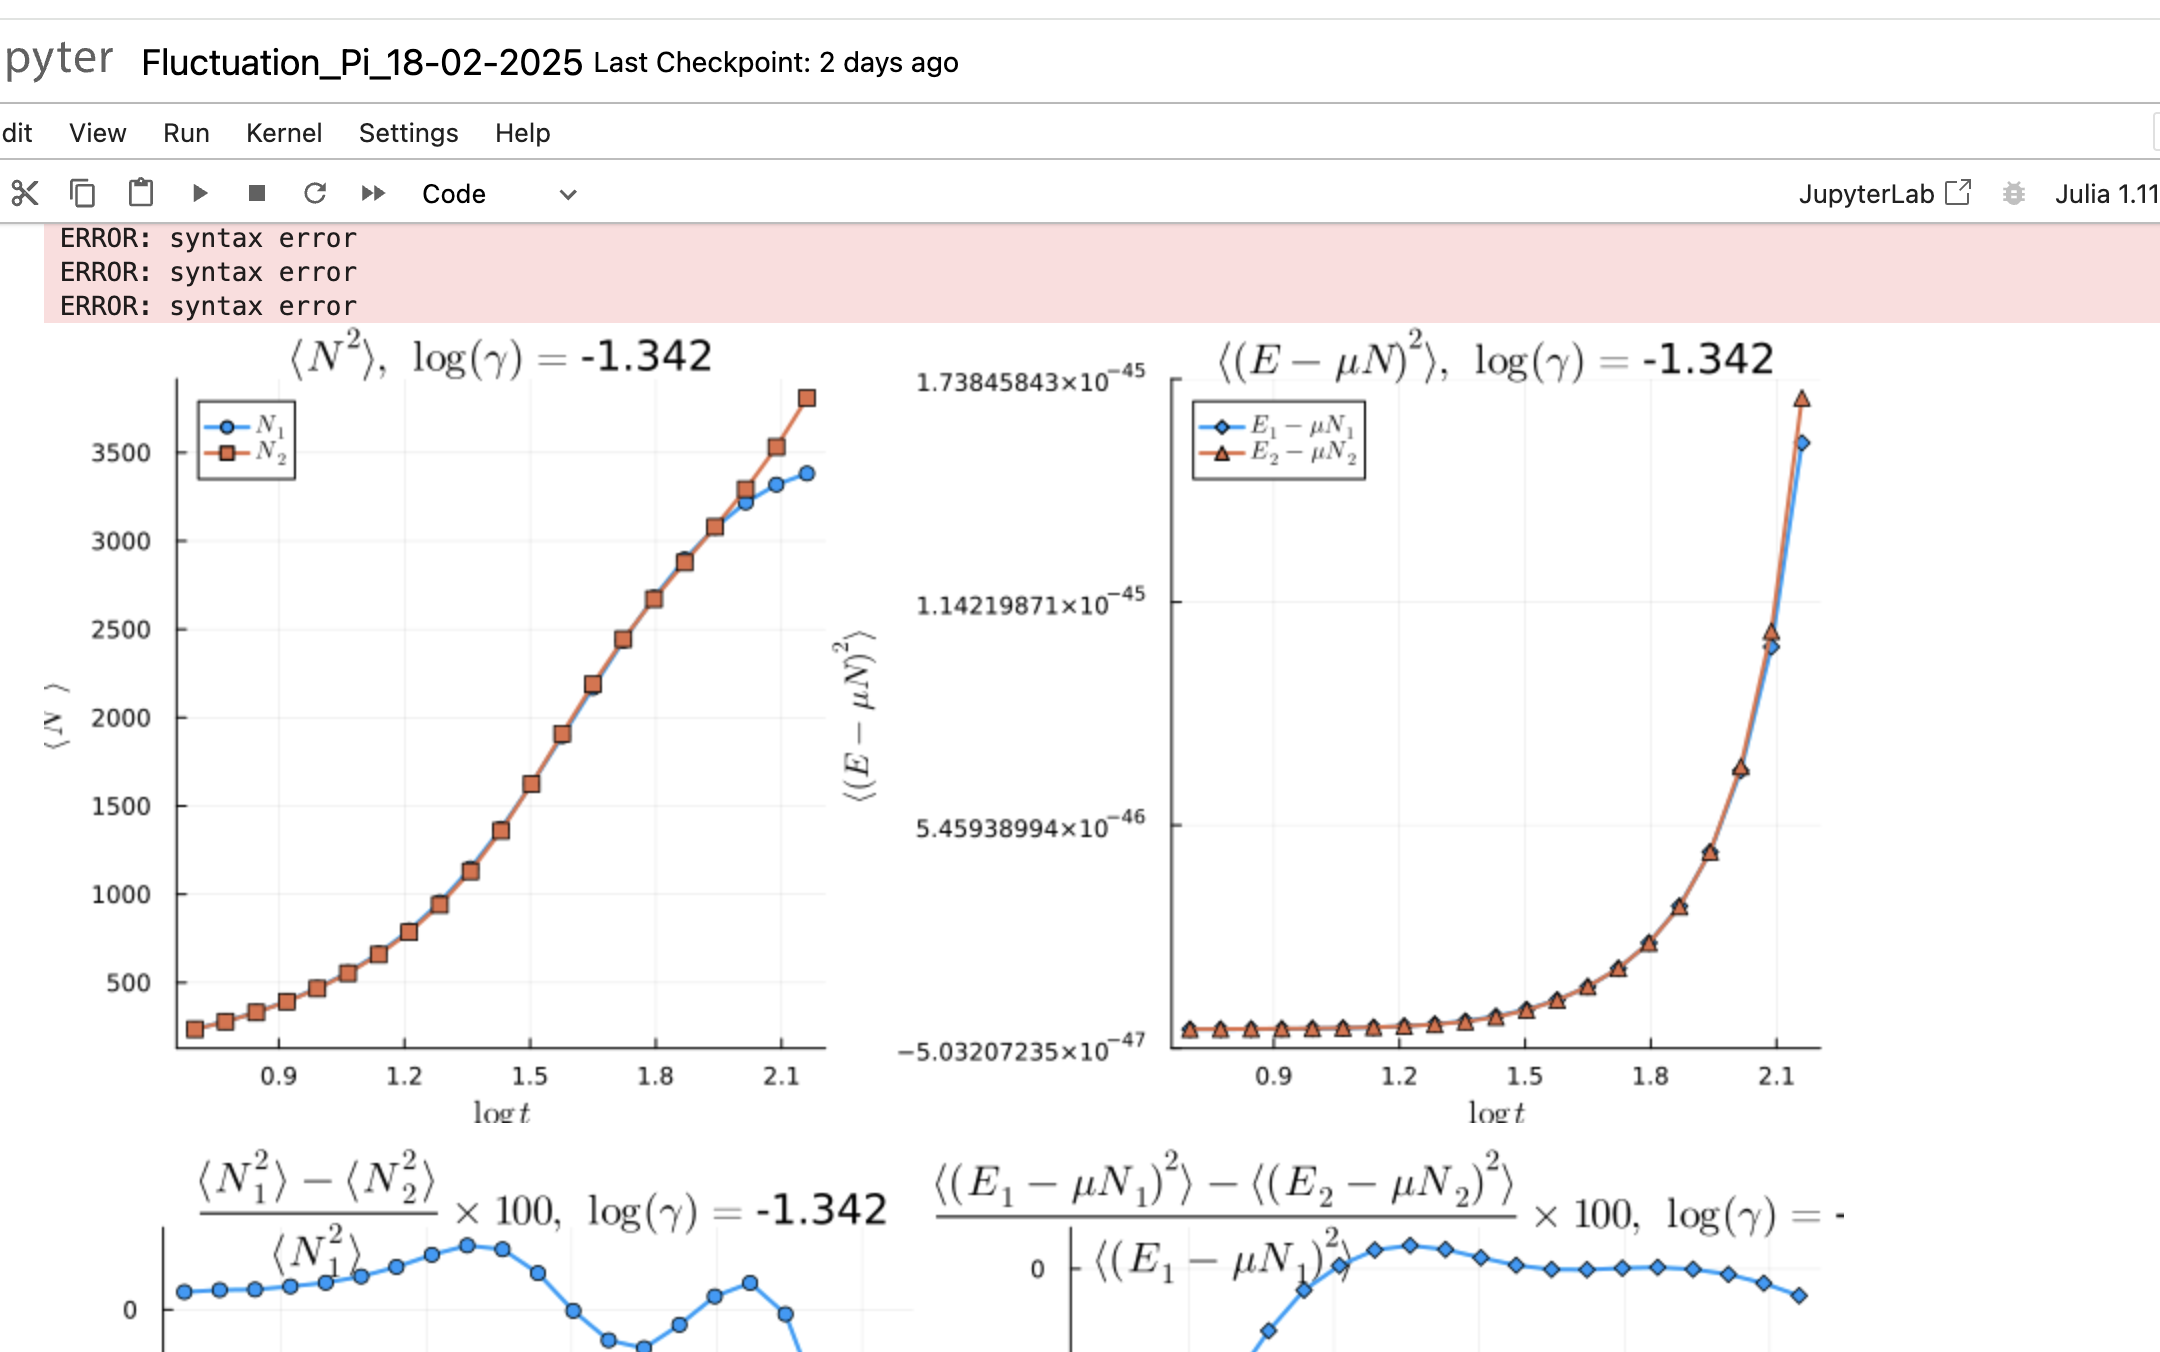
\includegraphics[width=1\textwidth]{Figures/test}

%\begin{aff}
%Donc une a l'ordre un en $\delta \theta (\operator{A}^{(0)})^{-1} %\operator{V}$ 

%\begin{eqnarray*}
%	\langle \delta \Pi ( \theta) \delta \Pi ( \theta') \rangle & = &  ( (\Pi^c_s - \Pi^c)\Pi^c/\Pi^c_s ) ( \theta ) \delta_{\theta, \theta'}/\delta \theta + \mathscr{F}(\theta , \theta' ) ,	
%\end{eqnarray*}

%avec 

%\begin{eqnarray*}
%	\mathscr{F}(\theta , \theta' ) & = & \left [ (\Pi^c_s - \Pi^c )( \theta)  +  (\Pi^c_s - \Pi^c ) ( \theta' )\right ] \frac{\Pi^c}{\Pi^c_s}(\theta)\frac{\Pi^c}{\Pi^c_s}(\theta') \frac{ \Delta( \theta'- \theta )}{ 2 \pi }\\
%	&&  - \left [ (\Pi^c_s - \Pi^c )( \theta)   (\Pi^c_s - \Pi^c ) ( \theta' )\right ] \frac{\Pi^c}{\Pi^c_s}(\theta)\frac{\Pi^c}{\Pi^c_s}(\theta')\int d\theta'' \left (   \frac{ \Pi^c/\Pi^c_s}{\Pi^c_s - \Pi^c} \right )(\theta'') \frac{\Delta(\theta''- \theta)}{2 \pi}\frac{\Delta(\theta''- \theta')}{2 \pi}  	
%\end{eqnarray*}
%\end{aff}



 









\subsection{Exemple : action de $\operator{P}$ sur l’état $\vert \psi_N\rangle$}
%Dans ce chapitre, nous nous intéressons aux fluctuations de la distribution de rapidité \( \delta \rho \) autour d'une distribution de référence \( \rho^c \), qui maximise la contribution à la fonction de partition des états, exprimée comme une fonctionnelle de la distribution \( \rho \) : 

La fonction de partition des états, s'exprime comme une fonctionnelle de la distribution \( \rho \) : 

\begin{eqnarray*}
	\Xi & = & \sum_\rho \exp \left( -\mathcal{A}(\rho) \right).
\end{eqnarray*}  

Dans la section {\em \bf Entropie de Yang-Yang} (\ref{??}), l'action \( \mathcal{A}(\rho) \) s'écrit sous la forme :  

\begin{eqnarray*}
	\mathcal{A}(\rho) & \doteq & - L\mathcal{S}_{YY}(\rho) + L\int f(\theta) \rho (\theta) \, d\theta,		
\end{eqnarray*}  

où \( \mathcal{S}_{YY} \) est la fonctionnelle d'entropie de Yang-Yang, définie dans (\ref{??}), et \( f \) est la fonction paramétrant les charges, introduite dans (\ref{??}).  

Dans cette même section {\em \bf Entropie de Yang-Yang} (\ref{??}), nous avons établi un lien entre \( f \) et distribution de référence \( \rho^c \), qui maximise la contribution à la fonction de partition des états .\\

On veux tester si nos experience est décrit pas un GGE. Pour cela nous nous intéressons aux fluctuations de la distribution de rapidité \( \delta \rho \) autour \( \rho^c \).

%Nous poursuivons à présent avec cette définition de l'action de classe $\mathcal{C}^2$ et admetant une distribution critique $\rho^c$ tel que sa différentielle en ce point critique soit nulle $d\mathcal{A}_{\rho^c} = 0 $ (\ref{??}) de sorte que d'aprés la formule de Taylor-Youg %afin de déterminer les fluctuations autour de \( \Pi^c \). Pour cela, nous réécrivons l'action sous la forme :  

Nous poursuivons à présent avec cette définition de l'action de classe $\mathcal{C}^2$ et admetant une distribution critique $\rho^c$ tel que sa différentielle en ce point critique soit nulle $d\mathcal{A}_{\rho^c} = 0 $ (\ref{??}) de sorte que d'aprés la formule de Taylor-Youg %afin de déterminer les fluctuations autour de \( \Pi^c \). Pour cela, nous réécrivons l'action sous la forme :  

\begin{eqnarray*}  
	\mathcal{A}(\rho^c + \delta \rho) & \underset{ \delta \rho \to 0 }{=} & \mathcal{A}(\rho^c)  + \frac{1}{2} \left. \frac{\delta^2 \mathcal{A}}{\delta \rho^2} \right|_{\rho^c} (\delta \rho) + \mathcal{O}((\delta \rho)^3),  
\end{eqnarray*}  

une expression quadratique pour l'action à l'ordre dominant en \( \delta \Pi \) avec $\left. \frac{\delta^2 \mathcal{A}}{\delta \rho^2} \right|_{\rho^c}$ la forme quadratique définie positive (Fig (\ref{fig.fluctu.A})).

\begin{figure}[H]
	\centering 
	\begin{tikzpicture}
		\begin{scope}[shift={(0,0)}]
			\begin{scope}[transform canvas={scale=0.6}]
				\input{Figures/Fonc_A_code}	
			
			\end{scope}
			
			\draw[color = red , scale = 0.5 , draw = none  ] (-2 , -1) rectangle (5, 6) ; 	
		\end{scope}
		
		\begin{scope}[shift={(19,-1)}]
			\begin{scope}[transform canvas={scale=0.6}]
				\input{Figures/Occupation_theta_code}	
			
			\end{scope}
			\begin{scope}[scale=1]
				\draw[color = red , scale = 1 , draw = none  ] (-1 , -1) rectangle (5, 5) ; 
			\end{scope}	
		\end{scope}

		
				
			
	\end{tikzpicture}	
	\captionsetup{skip=10pt} % Ajoute de l’espace après la légende
	\label{fig.fluctu.A}
\end{figure}


On discrétise l'axe des rapidités en  petite cellule de rapidité $[\theta, \theta+\delta\theta]$, qui contient $L\rho(\theta) \delta \theta$ rapidités. 
	



Avec ces petites tranches, la forme quadratique s’écrit :

\begin{eqnarray*}
    \left. \frac{\delta^2 \mathcal{A}}{{\delta \rho}^2} \right|_{\rho^c}(\delta \rho ) &=&  \sum_{a,b \mid \text{tranche}}  
    \delta \rho(\theta_a)  \frac{\partial^2 \mathcal{A}}{\partial \delta \rho(\theta_a) \partial \delta \rho(\theta_b) } (\rho^c)  \delta \rho(\theta_b).
\end{eqnarray*}
Les fluctuations s’écrivent donc :

\begin{eqnarray*}
    \langle \delta \rho ( \theta) \delta \rho ( \theta') \rangle &=&  
    \frac{ \int d\delta \rho \, \delta \rho(\theta) \delta \rho ( \theta') 
    \exp \left( - \frac{1}{2} \sum_{a,b \mid \text{tranche}}  
    \delta \rho(\theta_a) \frac{\partial^2 \mathcal{A}}{\partial \delta \rho(\theta_a) \partial \delta \rho(\theta_b) } (\rho^c)  \delta \rho(\theta_b) \right) }
    { \int d\delta \Pi  
    \exp \left( - \frac{1}{2} \sum_{a,b \mid \text{tranche}}  
    \delta \rho(\theta_a) \frac{\partial^2 \mathcal{A}}{\partial \delta \rho(\theta_a) \partial \delta \rho(\theta_b) } (\rho^c)  \delta \rho(\theta_b) \right) } \\
    &=& \left( \mathbf{A}^{-1} \right)_{\theta , \theta'}
\end{eqnarray*}


\begin{aff}

\begin{eqnarray*}
	\langle \delta \rho ( \theta) \delta \rho ( \theta') \rangle &=& 	\left( \mathbf{A}^{-1} \right)_{\theta , \theta'}
\end{eqnarray*}

	
avec la  {\em matrice hessienne} $\mathbf{A}_{\theta , \theta'} \equiv \frac{\partial^2 \mathcal{A}}{\partial \delta \rho(\theta) \partial \delta \rho(\theta') }(\rho^c)$, au point critique/ qui maximise la probabilité  $\rho^c=\rho^c_s \nu^c $, s'écrit

\begin{eqnarray*}
	\operator{A} & = & \operator{A}^{(0)} + \delta \theta \operator{V}
\end{eqnarray*}

avec 

\begin{eqnarray*}
	A^{(0)}_{\theta , \theta'}  & = &  L\delta \theta \left ( \frac{ 1}{\rho^c_s ( 1  - \nu^c ) \nu^c } \right )(\theta)    \delta({\theta - \theta '})	,\\
	V_{\theta , \theta'}  &= & L \delta \theta \left \{ - \left [ \left ( \frac{1}{\rho^c_s( 1 - \nu^c) } \right ) ( \theta)  +  \left ( \frac{1}{\rho^c_s( 1 - \nu^c) } \right ) ( \theta' )\right ] \frac{ \Delta( \theta'- \theta )}{ 2 \pi } + \int d\theta''  \left ( \frac{\nu^c}{\rho^c_s( 1 - \nu^c) } \right )(\theta'') \frac{\Delta(\theta''- \theta)}{2 \pi}\frac{\Delta(\theta''- \theta')}{2 \pi}   \right \} 	
\end{eqnarray*}

\end{aff}

\subsection{Testes}

\begin{eqnarray*}
	\Delta_{\operator{\mathcal{N}}}^2  & = &  \frac{1}{\beta} \left . \frac{\partial \langle \operator{\mathcal{N}} \rangle}{\partial \mu} \right )_T \\
	\Delta_{\operator{\mathcal{E}}-\mu \operator{\mathcal{N}}}^2  & = &  - \left . \frac{\partial \langle \operator{\mathcal{E}}-\mu \operator{\mathcal{N}} \rangle}{\partial \beta} \right )_\mu 
\end{eqnarray*}

et 

\begin{eqnarray*}
	\Delta_{\operator{\mathcal{N}}}^2  &= & L^2 \int d\theta_a \int d \theta_b \, \langle \delta \rho(\theta_a) \delta \rho(\theta_b) \rangle \\
	\Delta_{\operator{\mathcal{E}}-\mu \operator{\mathcal{N}}}^2  & = & L^2 \int d\theta_a \int d \theta_b \, \left ( - \mu + \frac{1}2 m \theta_a^2  \right  )\left ( - \mu + \frac{1}2 m \theta_b^2  \right  )  \langle \delta \rho(\theta_a) \delta \rho(\theta_b) \rangle
\end{eqnarray*}

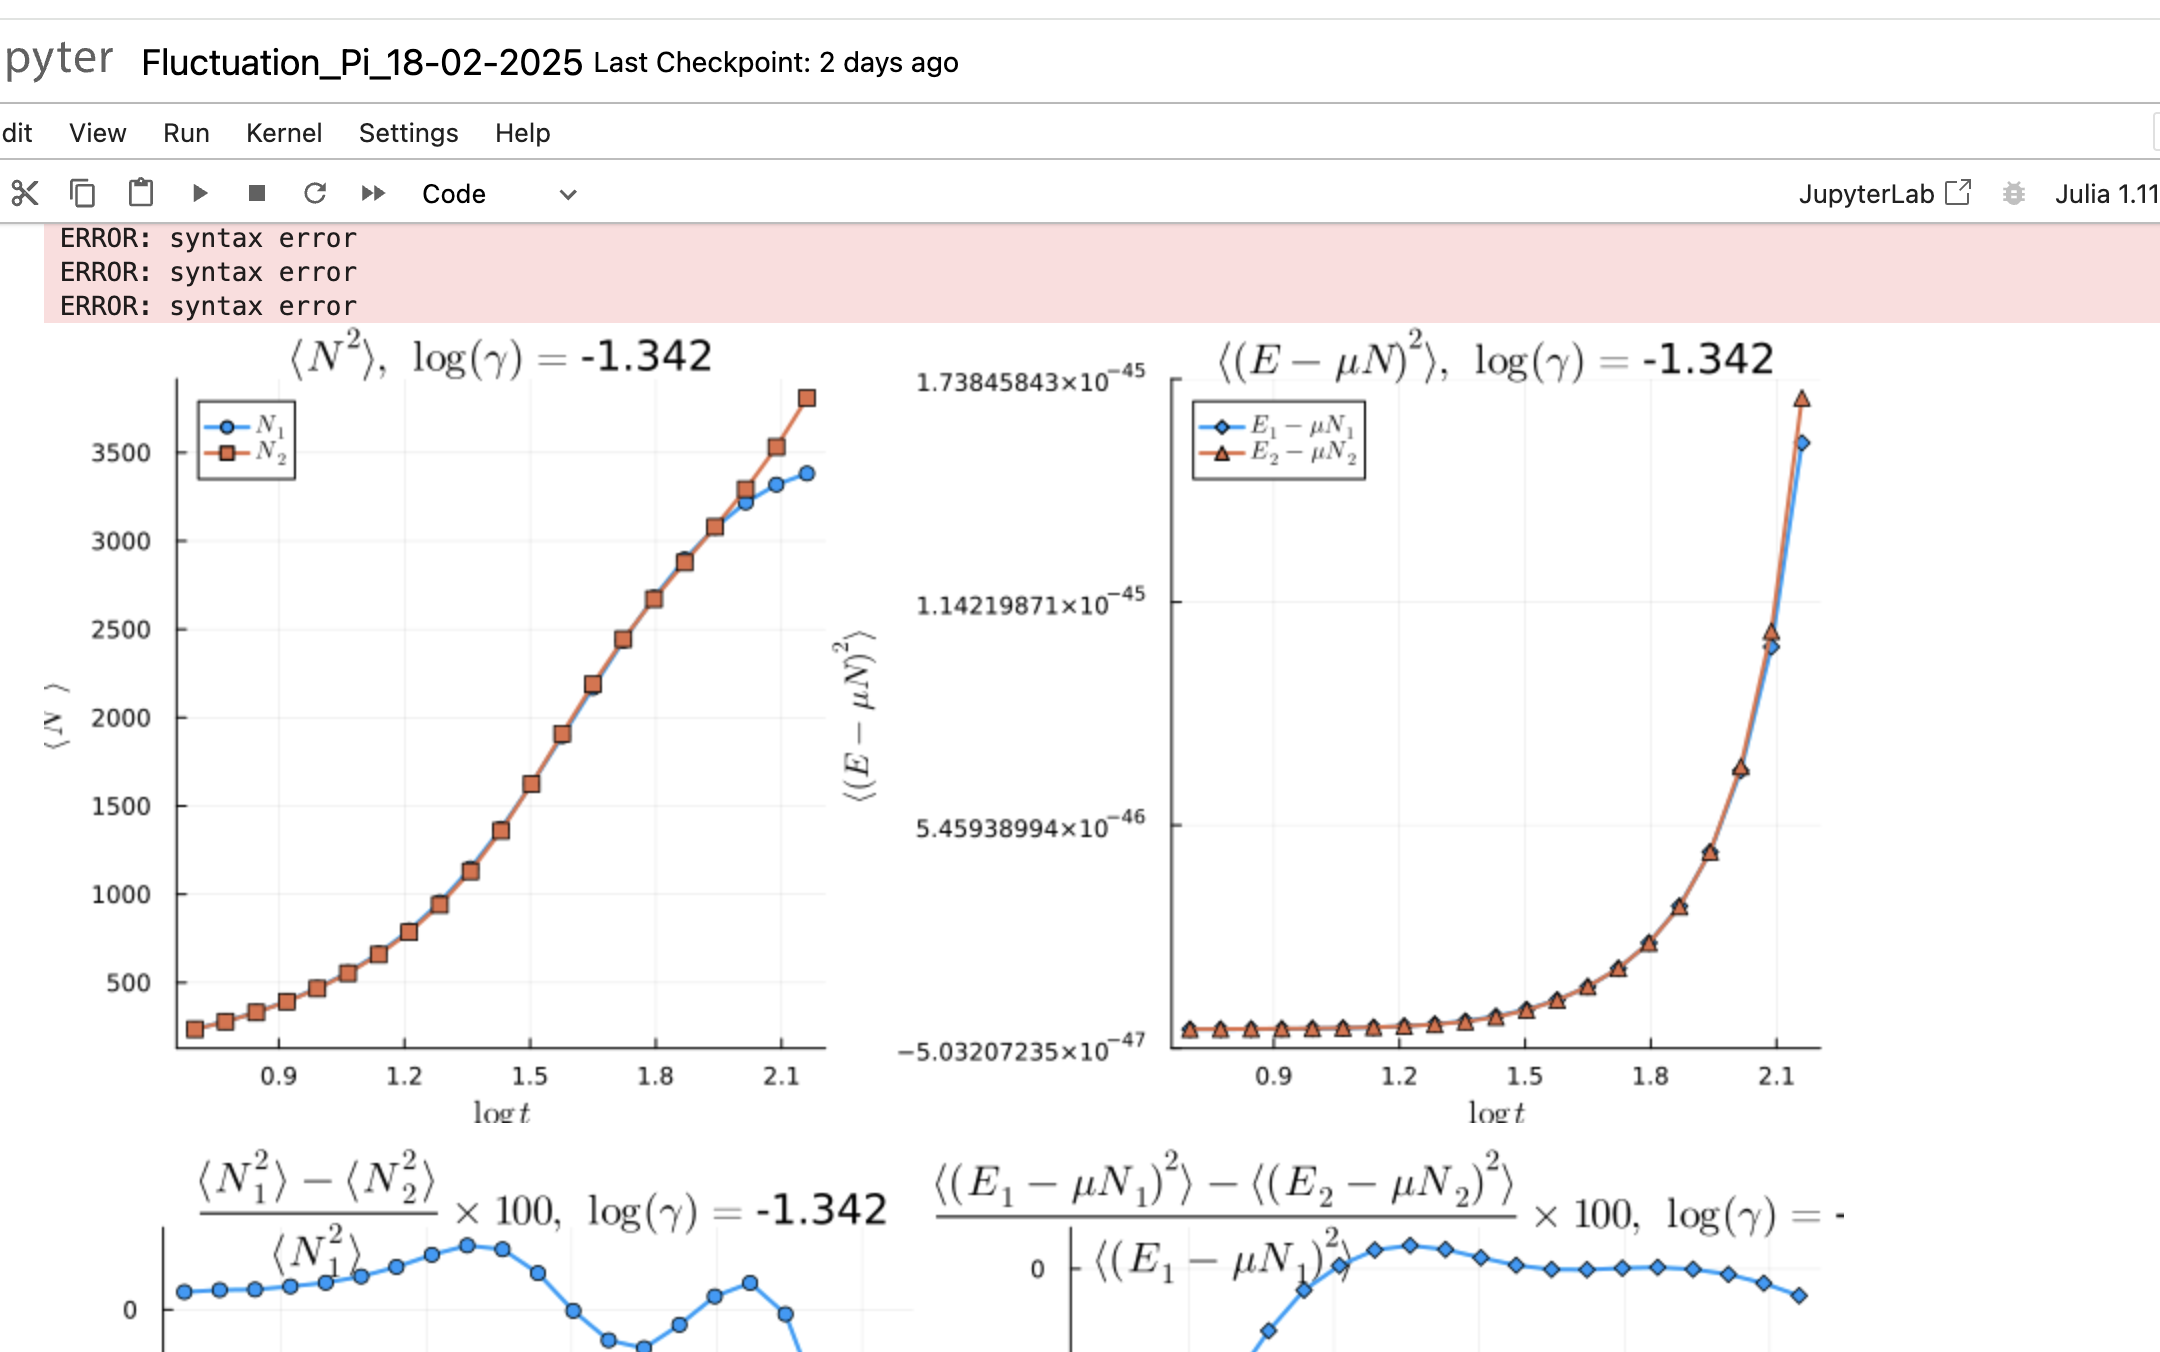
\includegraphics[width=1\textwidth]{Figures/test}

%\begin{aff}
%Donc une a l'ordre un en $\delta \theta (\operator{A}^{(0)})^{-1} %\operator{V}$ 

%\begin{eqnarray*}
%	\langle \delta \Pi ( \theta) \delta \Pi ( \theta') \rangle & = &  ( (\Pi^c_s - \Pi^c)\Pi^c/\Pi^c_s ) ( \theta ) \delta_{\theta, \theta'}/\delta \theta + \mathscr{F}(\theta , \theta' ) ,	
%\end{eqnarray*}

%avec 

%\begin{eqnarray*}
%	\mathscr{F}(\theta , \theta' ) & = & \left [ (\Pi^c_s - \Pi^c )( \theta)  +  (\Pi^c_s - \Pi^c ) ( \theta' )\right ] \frac{\Pi^c}{\Pi^c_s}(\theta)\frac{\Pi^c}{\Pi^c_s}(\theta') \frac{ \Delta( \theta'- \theta )}{ 2 \pi }\\
%	&&  - \left [ (\Pi^c_s - \Pi^c )( \theta)   (\Pi^c_s - \Pi^c ) ( \theta' )\right ] \frac{\Pi^c}{\Pi^c_s}(\theta)\frac{\Pi^c}{\Pi^c_s}(\theta')\int d\theta'' \left (   \frac{ \Pi^c/\Pi^c_s}{\Pi^c_s - \Pi^c} \right )(\theta'') \frac{\Delta(\theta''- \theta)}{2 \pi}\frac{\Delta(\theta''- \theta')}{2 \pi}  	
%\end{eqnarray*}
%\end{aff}



 









\subsection{Aaction de $\operator{H}$ sur l’état $\vert \psi_N\rangle$}
%Dans ce chapitre, nous nous intéressons aux fluctuations de la distribution de rapidité \( \delta \rho \) autour d'une distribution de référence \( \rho^c \), qui maximise la contribution à la fonction de partition des états, exprimée comme une fonctionnelle de la distribution \( \rho \) : 

La fonction de partition des états, s'exprime comme une fonctionnelle de la distribution \( \rho \) : 

\begin{eqnarray*}
	\Xi & = & \sum_\rho \exp \left( -\mathcal{A}(\rho) \right).
\end{eqnarray*}  

Dans la section {\em \bf Entropie de Yang-Yang} (\ref{??}), l'action \( \mathcal{A}(\rho) \) s'écrit sous la forme :  

\begin{eqnarray*}
	\mathcal{A}(\rho) & \doteq & - L\mathcal{S}_{YY}(\rho) + L\int f(\theta) \rho (\theta) \, d\theta,		
\end{eqnarray*}  

où \( \mathcal{S}_{YY} \) est la fonctionnelle d'entropie de Yang-Yang, définie dans (\ref{??}), et \( f \) est la fonction paramétrant les charges, introduite dans (\ref{??}).  

Dans cette même section {\em \bf Entropie de Yang-Yang} (\ref{??}), nous avons établi un lien entre \( f \) et distribution de référence \( \rho^c \), qui maximise la contribution à la fonction de partition des états .\\

On veux tester si nos experience est décrit pas un GGE. Pour cela nous nous intéressons aux fluctuations de la distribution de rapidité \( \delta \rho \) autour \( \rho^c \).

%Nous poursuivons à présent avec cette définition de l'action de classe $\mathcal{C}^2$ et admetant une distribution critique $\rho^c$ tel que sa différentielle en ce point critique soit nulle $d\mathcal{A}_{\rho^c} = 0 $ (\ref{??}) de sorte que d'aprés la formule de Taylor-Youg %afin de déterminer les fluctuations autour de \( \Pi^c \). Pour cela, nous réécrivons l'action sous la forme :  

Nous poursuivons à présent avec cette définition de l'action de classe $\mathcal{C}^2$ et admetant une distribution critique $\rho^c$ tel que sa différentielle en ce point critique soit nulle $d\mathcal{A}_{\rho^c} = 0 $ (\ref{??}) de sorte que d'aprés la formule de Taylor-Youg %afin de déterminer les fluctuations autour de \( \Pi^c \). Pour cela, nous réécrivons l'action sous la forme :  

\begin{eqnarray*}  
	\mathcal{A}(\rho^c + \delta \rho) & \underset{ \delta \rho \to 0 }{=} & \mathcal{A}(\rho^c)  + \frac{1}{2} \left. \frac{\delta^2 \mathcal{A}}{\delta \rho^2} \right|_{\rho^c} (\delta \rho) + \mathcal{O}((\delta \rho)^3),  
\end{eqnarray*}  

une expression quadratique pour l'action à l'ordre dominant en \( \delta \Pi \) avec $\left. \frac{\delta^2 \mathcal{A}}{\delta \rho^2} \right|_{\rho^c}$ la forme quadratique définie positive (Fig (\ref{fig.fluctu.A})).

\begin{figure}[H]
	\centering 
	\begin{tikzpicture}
		\begin{scope}[shift={(0,0)}]
			\begin{scope}[transform canvas={scale=0.6}]
				\input{Figures/Fonc_A_code}	
			
			\end{scope}
			
			\draw[color = red , scale = 0.5 , draw = none  ] (-2 , -1) rectangle (5, 6) ; 	
		\end{scope}
		
		\begin{scope}[shift={(19,-1)}]
			\begin{scope}[transform canvas={scale=0.6}]
				\input{Figures/Occupation_theta_code}	
			
			\end{scope}
			\begin{scope}[scale=1]
				\draw[color = red , scale = 1 , draw = none  ] (-1 , -1) rectangle (5, 5) ; 
			\end{scope}	
		\end{scope}

		
				
			
	\end{tikzpicture}	
	\captionsetup{skip=10pt} % Ajoute de l’espace après la légende
	\label{fig.fluctu.A}
\end{figure}


On discrétise l'axe des rapidités en  petite cellule de rapidité $[\theta, \theta+\delta\theta]$, qui contient $L\rho(\theta) \delta \theta$ rapidités. 
	



Avec ces petites tranches, la forme quadratique s’écrit :

\begin{eqnarray*}
    \left. \frac{\delta^2 \mathcal{A}}{{\delta \rho}^2} \right|_{\rho^c}(\delta \rho ) &=&  \sum_{a,b \mid \text{tranche}}  
    \delta \rho(\theta_a)  \frac{\partial^2 \mathcal{A}}{\partial \delta \rho(\theta_a) \partial \delta \rho(\theta_b) } (\rho^c)  \delta \rho(\theta_b).
\end{eqnarray*}
Les fluctuations s’écrivent donc :

\begin{eqnarray*}
    \langle \delta \rho ( \theta) \delta \rho ( \theta') \rangle &=&  
    \frac{ \int d\delta \rho \, \delta \rho(\theta) \delta \rho ( \theta') 
    \exp \left( - \frac{1}{2} \sum_{a,b \mid \text{tranche}}  
    \delta \rho(\theta_a) \frac{\partial^2 \mathcal{A}}{\partial \delta \rho(\theta_a) \partial \delta \rho(\theta_b) } (\rho^c)  \delta \rho(\theta_b) \right) }
    { \int d\delta \Pi  
    \exp \left( - \frac{1}{2} \sum_{a,b \mid \text{tranche}}  
    \delta \rho(\theta_a) \frac{\partial^2 \mathcal{A}}{\partial \delta \rho(\theta_a) \partial \delta \rho(\theta_b) } (\rho^c)  \delta \rho(\theta_b) \right) } \\
    &=& \left( \mathbf{A}^{-1} \right)_{\theta , \theta'}
\end{eqnarray*}


\begin{aff}

\begin{eqnarray*}
	\langle \delta \rho ( \theta) \delta \rho ( \theta') \rangle &=& 	\left( \mathbf{A}^{-1} \right)_{\theta , \theta'}
\end{eqnarray*}

	
avec la  {\em matrice hessienne} $\mathbf{A}_{\theta , \theta'} \equiv \frac{\partial^2 \mathcal{A}}{\partial \delta \rho(\theta) \partial \delta \rho(\theta') }(\rho^c)$, au point critique/ qui maximise la probabilité  $\rho^c=\rho^c_s \nu^c $, s'écrit

\begin{eqnarray*}
	\operator{A} & = & \operator{A}^{(0)} + \delta \theta \operator{V}
\end{eqnarray*}

avec 

\begin{eqnarray*}
	A^{(0)}_{\theta , \theta'}  & = &  L\delta \theta \left ( \frac{ 1}{\rho^c_s ( 1  - \nu^c ) \nu^c } \right )(\theta)    \delta({\theta - \theta '})	,\\
	V_{\theta , \theta'}  &= & L \delta \theta \left \{ - \left [ \left ( \frac{1}{\rho^c_s( 1 - \nu^c) } \right ) ( \theta)  +  \left ( \frac{1}{\rho^c_s( 1 - \nu^c) } \right ) ( \theta' )\right ] \frac{ \Delta( \theta'- \theta )}{ 2 \pi } + \int d\theta''  \left ( \frac{\nu^c}{\rho^c_s( 1 - \nu^c) } \right )(\theta'') \frac{\Delta(\theta''- \theta)}{2 \pi}\frac{\Delta(\theta''- \theta')}{2 \pi}   \right \} 	
\end{eqnarray*}

\end{aff}

\subsection{Testes}

\begin{eqnarray*}
	\Delta_{\operator{\mathcal{N}}}^2  & = &  \frac{1}{\beta} \left . \frac{\partial \langle \operator{\mathcal{N}} \rangle}{\partial \mu} \right )_T \\
	\Delta_{\operator{\mathcal{E}}-\mu \operator{\mathcal{N}}}^2  & = &  - \left . \frac{\partial \langle \operator{\mathcal{E}}-\mu \operator{\mathcal{N}} \rangle}{\partial \beta} \right )_\mu 
\end{eqnarray*}

et 

\begin{eqnarray*}
	\Delta_{\operator{\mathcal{N}}}^2  &= & L^2 \int d\theta_a \int d \theta_b \, \langle \delta \rho(\theta_a) \delta \rho(\theta_b) \rangle \\
	\Delta_{\operator{\mathcal{E}}-\mu \operator{\mathcal{N}}}^2  & = & L^2 \int d\theta_a \int d \theta_b \, \left ( - \mu + \frac{1}2 m \theta_a^2  \right  )\left ( - \mu + \frac{1}2 m \theta_b^2  \right  )  \langle \delta \rho(\theta_a) \delta \rho(\theta_b) \rangle
\end{eqnarray*}

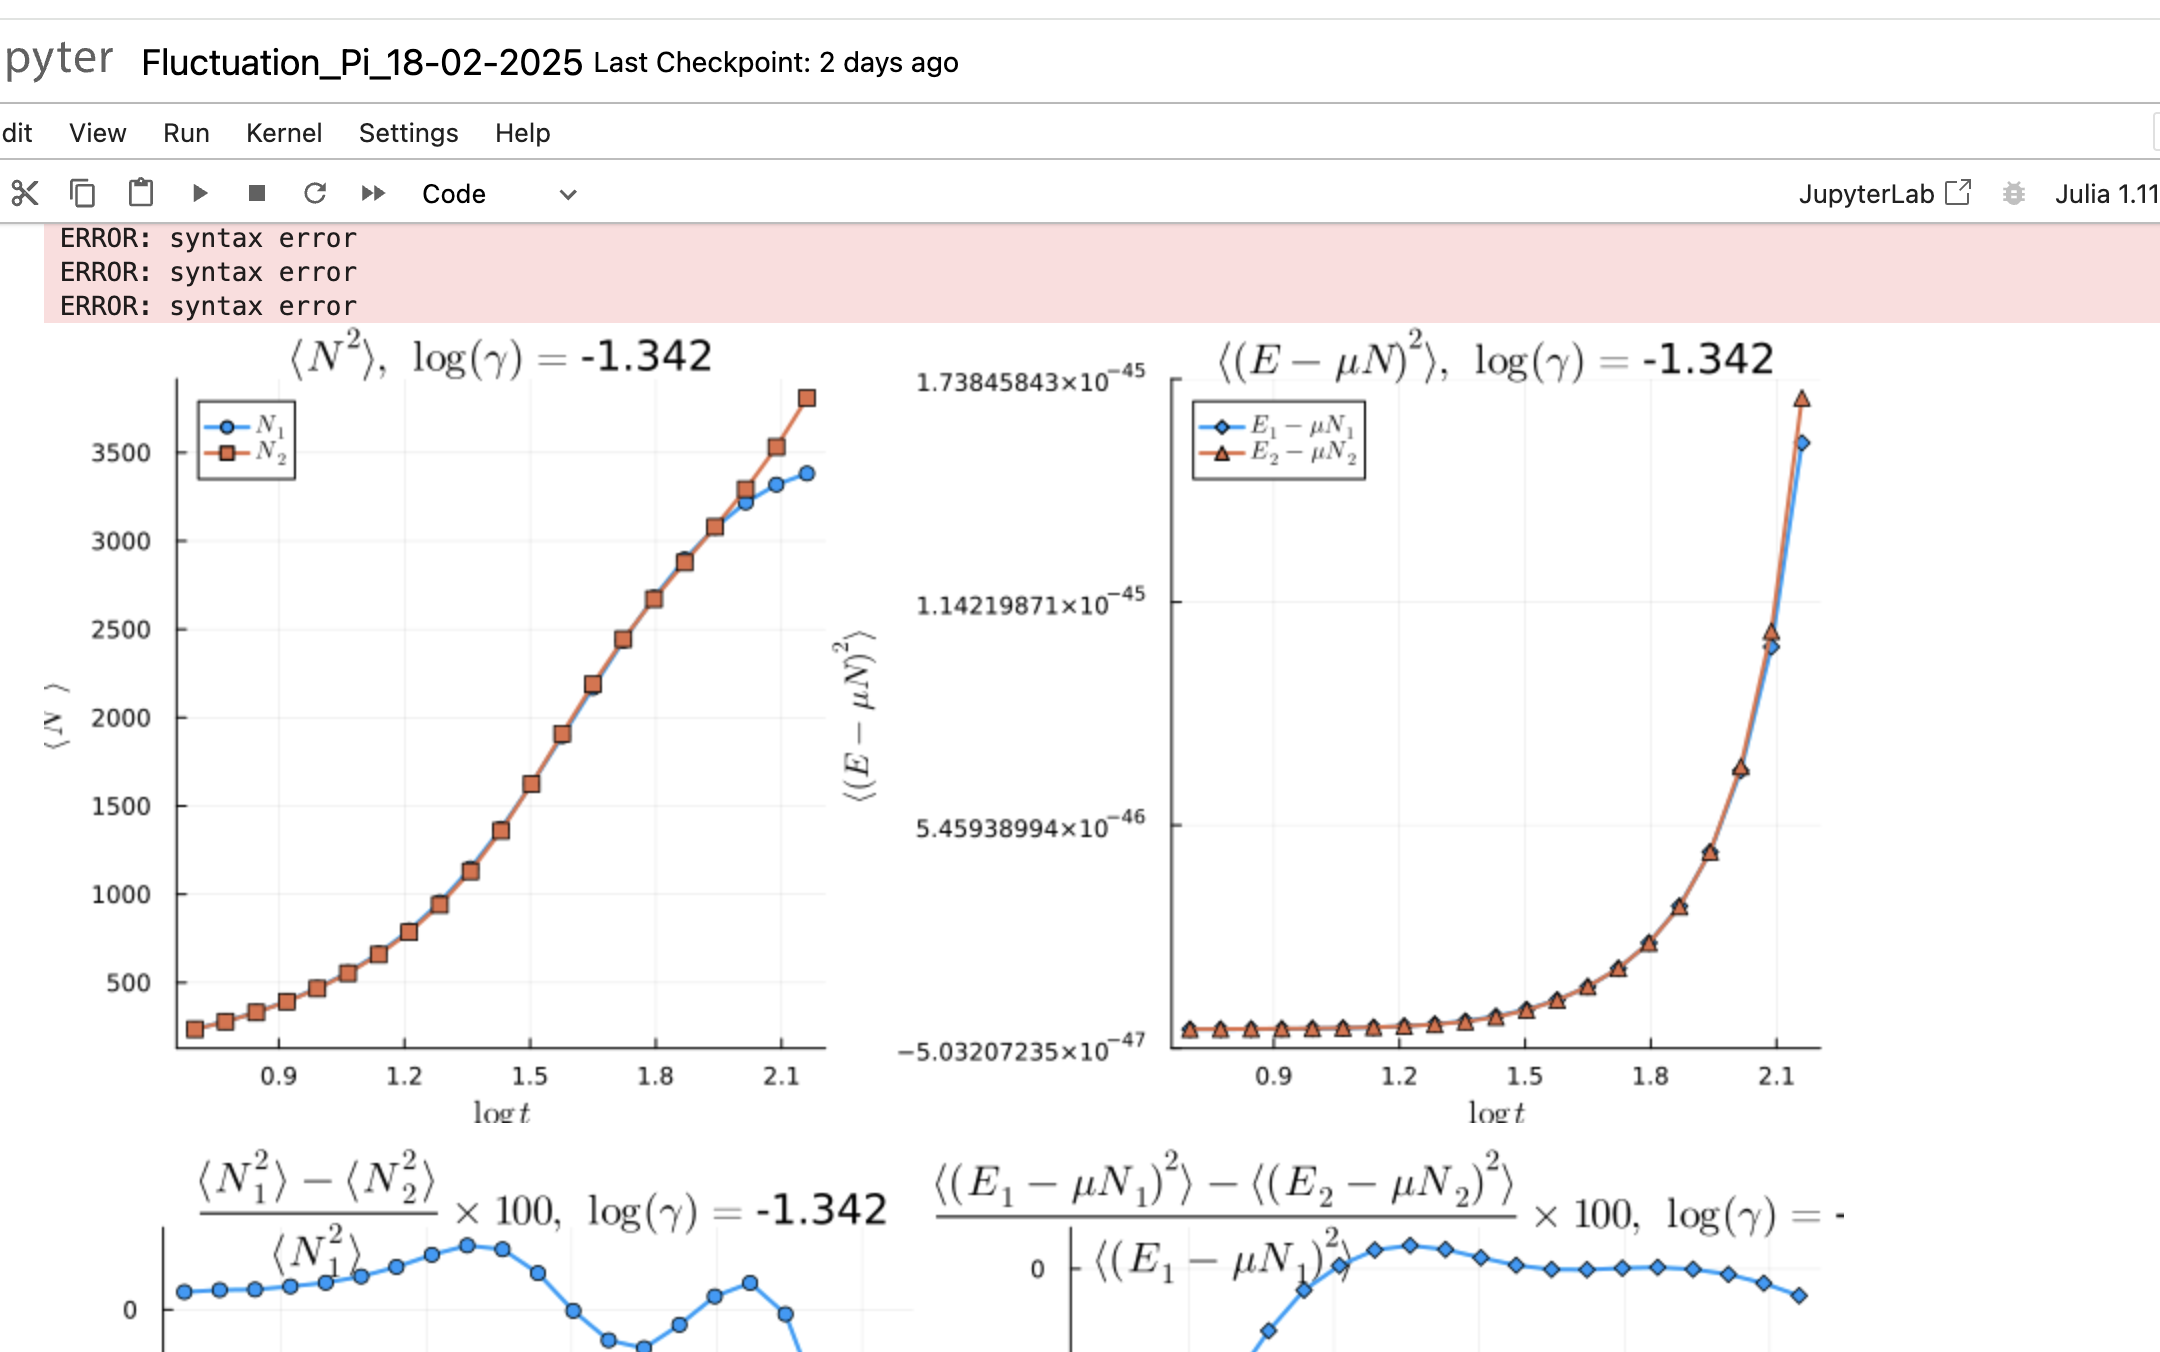
\includegraphics[width=1\textwidth]{Figures/test}

%\begin{aff}
%Donc une a l'ordre un en $\delta \theta (\operator{A}^{(0)})^{-1} %\operator{V}$ 

%\begin{eqnarray*}
%	\langle \delta \Pi ( \theta) \delta \Pi ( \theta') \rangle & = &  ( (\Pi^c_s - \Pi^c)\Pi^c/\Pi^c_s ) ( \theta ) \delta_{\theta, \theta'}/\delta \theta + \mathscr{F}(\theta , \theta' ) ,	
%\end{eqnarray*}

%avec 

%\begin{eqnarray*}
%	\mathscr{F}(\theta , \theta' ) & = & \left [ (\Pi^c_s - \Pi^c )( \theta)  +  (\Pi^c_s - \Pi^c ) ( \theta' )\right ] \frac{\Pi^c}{\Pi^c_s}(\theta)\frac{\Pi^c}{\Pi^c_s}(\theta') \frac{ \Delta( \theta'- \theta )}{ 2 \pi }\\
%	&&  - \left [ (\Pi^c_s - \Pi^c )( \theta)   (\Pi^c_s - \Pi^c ) ( \theta' )\right ] \frac{\Pi^c}{\Pi^c_s}(\theta)\frac{\Pi^c}{\Pi^c_s}(\theta')\int d\theta'' \left (   \frac{ \Pi^c/\Pi^c_s}{\Pi^c_s - \Pi^c} \right )(\theta'') \frac{\Delta(\theta''- \theta)}{2 \pi}\frac{\Delta(\theta''- \theta')}{2 \pi}  	
%\end{eqnarray*}
%\end{aff}



 









\subsection{Vérification explicite de la condition aux limites}
%Dans ce chapitre, nous nous intéressons aux fluctuations de la distribution de rapidité \( \delta \rho \) autour d'une distribution de référence \( \rho^c \), qui maximise la contribution à la fonction de partition des états, exprimée comme une fonctionnelle de la distribution \( \rho \) : 

La fonction de partition des états, s'exprime comme une fonctionnelle de la distribution \( \rho \) : 

\begin{eqnarray*}
	\Xi & = & \sum_\rho \exp \left( -\mathcal{A}(\rho) \right).
\end{eqnarray*}  

Dans la section {\em \bf Entropie de Yang-Yang} (\ref{??}), l'action \( \mathcal{A}(\rho) \) s'écrit sous la forme :  

\begin{eqnarray*}
	\mathcal{A}(\rho) & \doteq & - L\mathcal{S}_{YY}(\rho) + L\int f(\theta) \rho (\theta) \, d\theta,		
\end{eqnarray*}  

où \( \mathcal{S}_{YY} \) est la fonctionnelle d'entropie de Yang-Yang, définie dans (\ref{??}), et \( f \) est la fonction paramétrant les charges, introduite dans (\ref{??}).  

Dans cette même section {\em \bf Entropie de Yang-Yang} (\ref{??}), nous avons établi un lien entre \( f \) et distribution de référence \( \rho^c \), qui maximise la contribution à la fonction de partition des états .\\

On veux tester si nos experience est décrit pas un GGE. Pour cela nous nous intéressons aux fluctuations de la distribution de rapidité \( \delta \rho \) autour \( \rho^c \).

%Nous poursuivons à présent avec cette définition de l'action de classe $\mathcal{C}^2$ et admetant une distribution critique $\rho^c$ tel que sa différentielle en ce point critique soit nulle $d\mathcal{A}_{\rho^c} = 0 $ (\ref{??}) de sorte que d'aprés la formule de Taylor-Youg %afin de déterminer les fluctuations autour de \( \Pi^c \). Pour cela, nous réécrivons l'action sous la forme :  

Nous poursuivons à présent avec cette définition de l'action de classe $\mathcal{C}^2$ et admetant une distribution critique $\rho^c$ tel que sa différentielle en ce point critique soit nulle $d\mathcal{A}_{\rho^c} = 0 $ (\ref{??}) de sorte que d'aprés la formule de Taylor-Youg %afin de déterminer les fluctuations autour de \( \Pi^c \). Pour cela, nous réécrivons l'action sous la forme :  

\begin{eqnarray*}  
	\mathcal{A}(\rho^c + \delta \rho) & \underset{ \delta \rho \to 0 }{=} & \mathcal{A}(\rho^c)  + \frac{1}{2} \left. \frac{\delta^2 \mathcal{A}}{\delta \rho^2} \right|_{\rho^c} (\delta \rho) + \mathcal{O}((\delta \rho)^3),  
\end{eqnarray*}  

une expression quadratique pour l'action à l'ordre dominant en \( \delta \Pi \) avec $\left. \frac{\delta^2 \mathcal{A}}{\delta \rho^2} \right|_{\rho^c}$ la forme quadratique définie positive (Fig (\ref{fig.fluctu.A})).

\begin{figure}[H]
	\centering 
	\begin{tikzpicture}
		\begin{scope}[shift={(0,0)}]
			\begin{scope}[transform canvas={scale=0.6}]
				\input{Figures/Fonc_A_code}	
			
			\end{scope}
			
			\draw[color = red , scale = 0.5 , draw = none  ] (-2 , -1) rectangle (5, 6) ; 	
		\end{scope}
		
		\begin{scope}[shift={(19,-1)}]
			\begin{scope}[transform canvas={scale=0.6}]
				\input{Figures/Occupation_theta_code}	
			
			\end{scope}
			\begin{scope}[scale=1]
				\draw[color = red , scale = 1 , draw = none  ] (-1 , -1) rectangle (5, 5) ; 
			\end{scope}	
		\end{scope}

		
				
			
	\end{tikzpicture}	
	\captionsetup{skip=10pt} % Ajoute de l’espace après la légende
	\label{fig.fluctu.A}
\end{figure}


On discrétise l'axe des rapidités en  petite cellule de rapidité $[\theta, \theta+\delta\theta]$, qui contient $L\rho(\theta) \delta \theta$ rapidités. 
	



Avec ces petites tranches, la forme quadratique s’écrit :

\begin{eqnarray*}
    \left. \frac{\delta^2 \mathcal{A}}{{\delta \rho}^2} \right|_{\rho^c}(\delta \rho ) &=&  \sum_{a,b \mid \text{tranche}}  
    \delta \rho(\theta_a)  \frac{\partial^2 \mathcal{A}}{\partial \delta \rho(\theta_a) \partial \delta \rho(\theta_b) } (\rho^c)  \delta \rho(\theta_b).
\end{eqnarray*}
Les fluctuations s’écrivent donc :

\begin{eqnarray*}
    \langle \delta \rho ( \theta) \delta \rho ( \theta') \rangle &=&  
    \frac{ \int d\delta \rho \, \delta \rho(\theta) \delta \rho ( \theta') 
    \exp \left( - \frac{1}{2} \sum_{a,b \mid \text{tranche}}  
    \delta \rho(\theta_a) \frac{\partial^2 \mathcal{A}}{\partial \delta \rho(\theta_a) \partial \delta \rho(\theta_b) } (\rho^c)  \delta \rho(\theta_b) \right) }
    { \int d\delta \Pi  
    \exp \left( - \frac{1}{2} \sum_{a,b \mid \text{tranche}}  
    \delta \rho(\theta_a) \frac{\partial^2 \mathcal{A}}{\partial \delta \rho(\theta_a) \partial \delta \rho(\theta_b) } (\rho^c)  \delta \rho(\theta_b) \right) } \\
    &=& \left( \mathbf{A}^{-1} \right)_{\theta , \theta'}
\end{eqnarray*}


\begin{aff}

\begin{eqnarray*}
	\langle \delta \rho ( \theta) \delta \rho ( \theta') \rangle &=& 	\left( \mathbf{A}^{-1} \right)_{\theta , \theta'}
\end{eqnarray*}

	
avec la  {\em matrice hessienne} $\mathbf{A}_{\theta , \theta'} \equiv \frac{\partial^2 \mathcal{A}}{\partial \delta \rho(\theta) \partial \delta \rho(\theta') }(\rho^c)$, au point critique/ qui maximise la probabilité  $\rho^c=\rho^c_s \nu^c $, s'écrit

\begin{eqnarray*}
	\operator{A} & = & \operator{A}^{(0)} + \delta \theta \operator{V}
\end{eqnarray*}

avec 

\begin{eqnarray*}
	A^{(0)}_{\theta , \theta'}  & = &  L\delta \theta \left ( \frac{ 1}{\rho^c_s ( 1  - \nu^c ) \nu^c } \right )(\theta)    \delta({\theta - \theta '})	,\\
	V_{\theta , \theta'}  &= & L \delta \theta \left \{ - \left [ \left ( \frac{1}{\rho^c_s( 1 - \nu^c) } \right ) ( \theta)  +  \left ( \frac{1}{\rho^c_s( 1 - \nu^c) } \right ) ( \theta' )\right ] \frac{ \Delta( \theta'- \theta )}{ 2 \pi } + \int d\theta''  \left ( \frac{\nu^c}{\rho^c_s( 1 - \nu^c) } \right )(\theta'') \frac{\Delta(\theta''- \theta)}{2 \pi}\frac{\Delta(\theta''- \theta')}{2 \pi}   \right \} 	
\end{eqnarray*}

\end{aff}

\subsection{Testes}

\begin{eqnarray*}
	\Delta_{\operator{\mathcal{N}}}^2  & = &  \frac{1}{\beta} \left . \frac{\partial \langle \operator{\mathcal{N}} \rangle}{\partial \mu} \right )_T \\
	\Delta_{\operator{\mathcal{E}}-\mu \operator{\mathcal{N}}}^2  & = &  - \left . \frac{\partial \langle \operator{\mathcal{E}}-\mu \operator{\mathcal{N}} \rangle}{\partial \beta} \right )_\mu 
\end{eqnarray*}

et 

\begin{eqnarray*}
	\Delta_{\operator{\mathcal{N}}}^2  &= & L^2 \int d\theta_a \int d \theta_b \, \langle \delta \rho(\theta_a) \delta \rho(\theta_b) \rangle \\
	\Delta_{\operator{\mathcal{E}}-\mu \operator{\mathcal{N}}}^2  & = & L^2 \int d\theta_a \int d \theta_b \, \left ( - \mu + \frac{1}2 m \theta_a^2  \right  )\left ( - \mu + \frac{1}2 m \theta_b^2  \right  )  \langle \delta \rho(\theta_a) \delta \rho(\theta_b) \rangle
\end{eqnarray*}

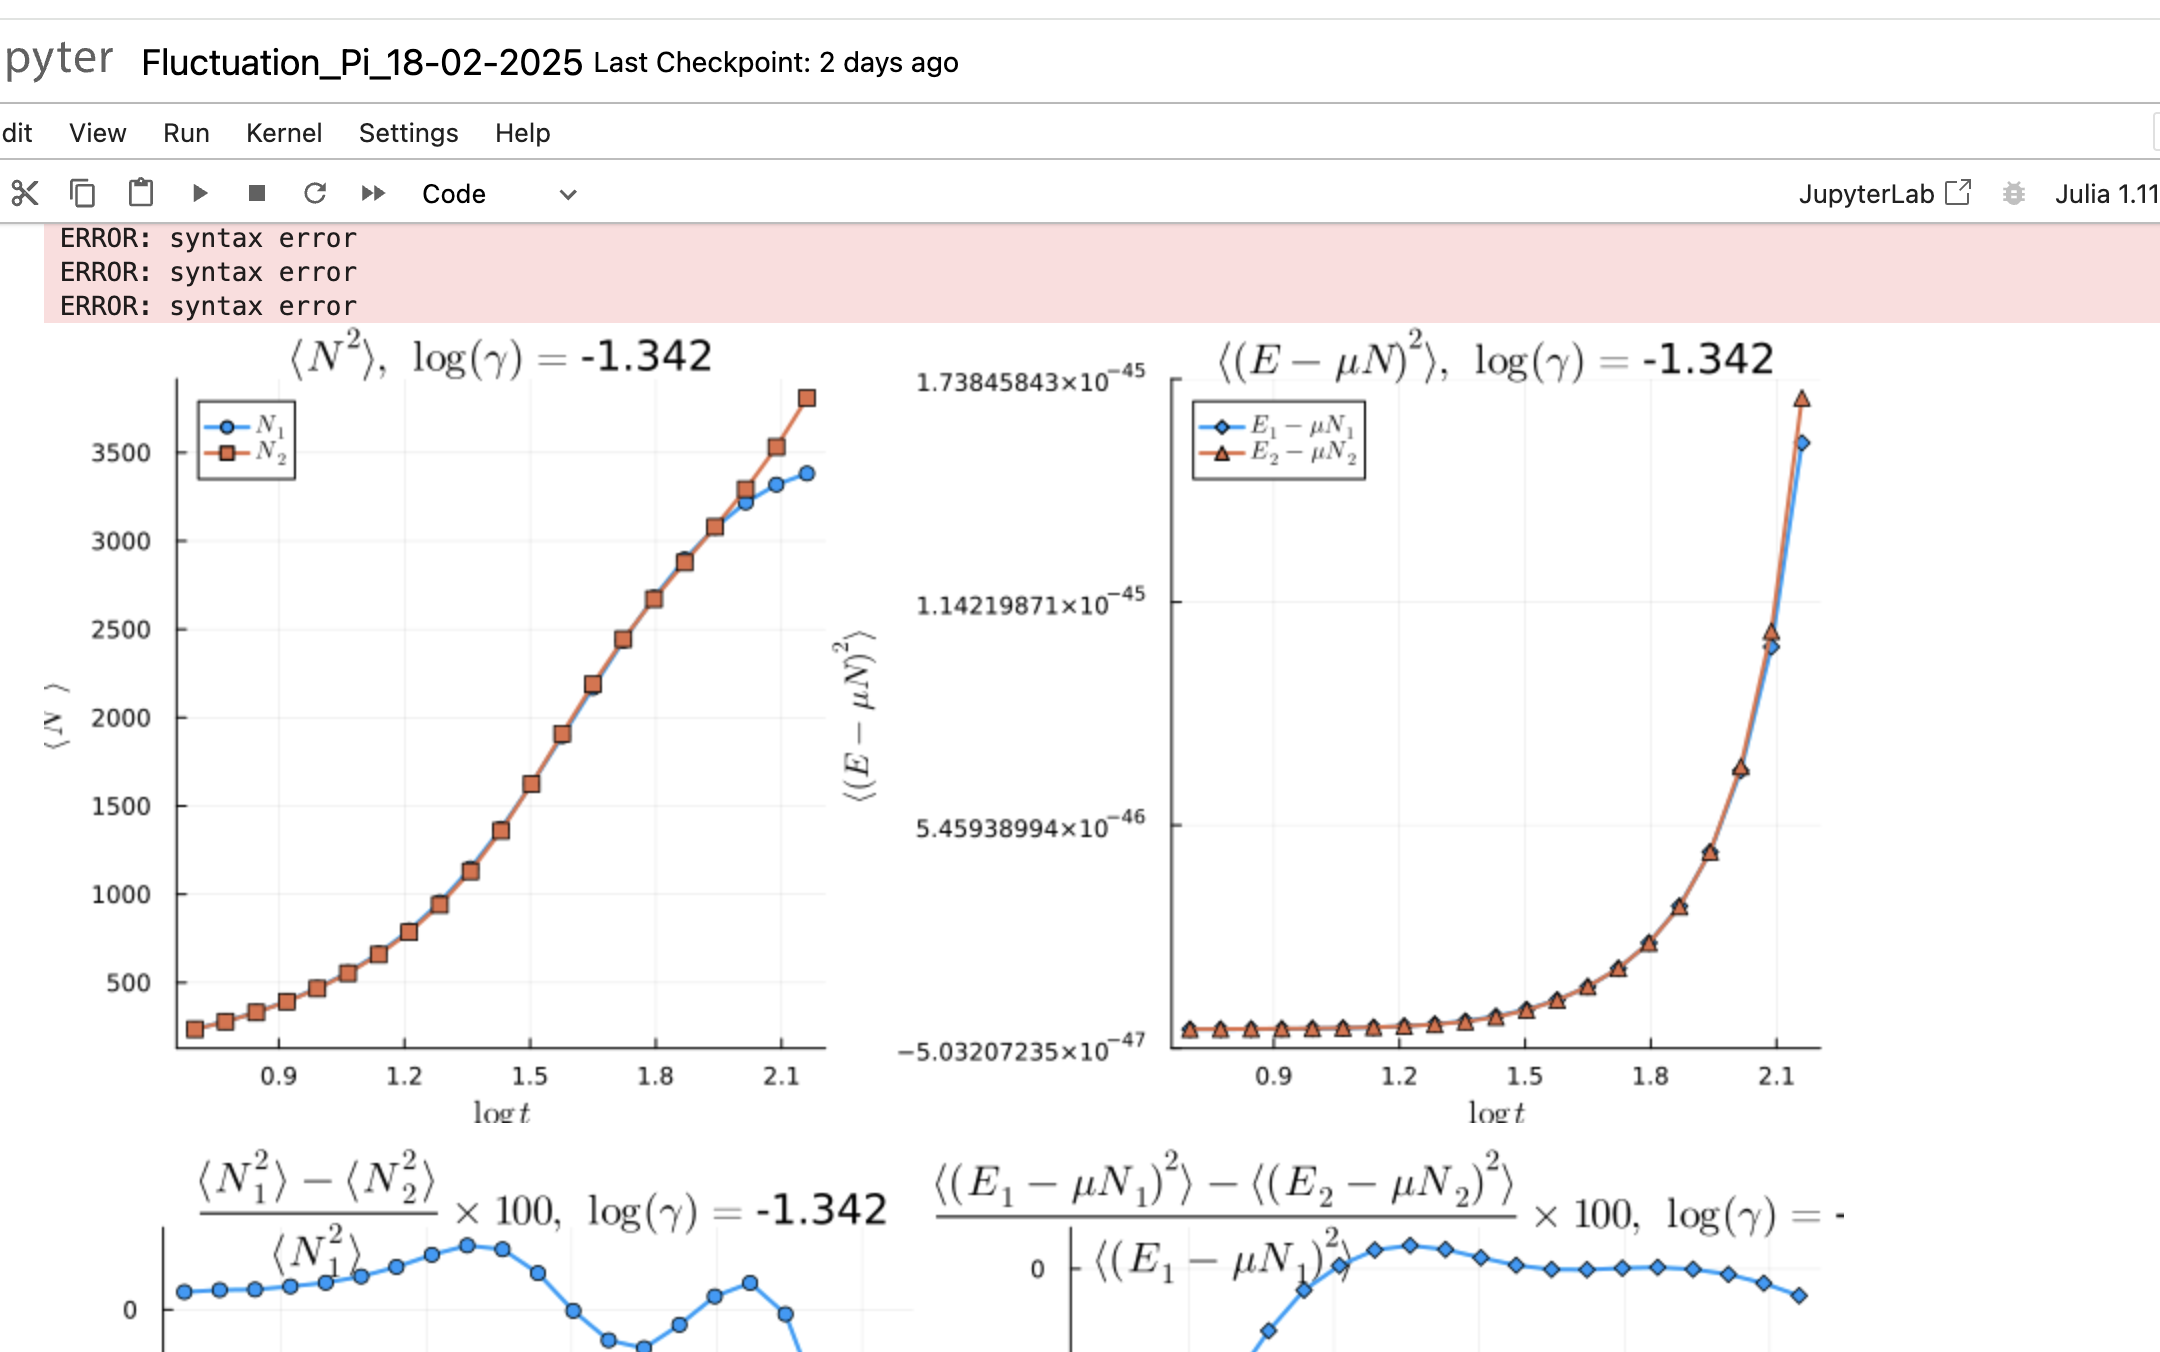
\includegraphics[width=1\textwidth]{Figures/test}

%\begin{aff}
%Donc une a l'ordre un en $\delta \theta (\operator{A}^{(0)})^{-1} %\operator{V}$ 

%\begin{eqnarray*}
%	\langle \delta \Pi ( \theta) \delta \Pi ( \theta') \rangle & = &  ( (\Pi^c_s - \Pi^c)\Pi^c/\Pi^c_s ) ( \theta ) \delta_{\theta, \theta'}/\delta \theta + \mathscr{F}(\theta , \theta' ) ,	
%\end{eqnarray*}

%avec 

%\begin{eqnarray*}
%	\mathscr{F}(\theta , \theta' ) & = & \left [ (\Pi^c_s - \Pi^c )( \theta)  +  (\Pi^c_s - \Pi^c ) ( \theta' )\right ] \frac{\Pi^c}{\Pi^c_s}(\theta)\frac{\Pi^c}{\Pi^c_s}(\theta') \frac{ \Delta( \theta'- \theta )}{ 2 \pi }\\
%	&&  - \left [ (\Pi^c_s - \Pi^c )( \theta)   (\Pi^c_s - \Pi^c ) ( \theta' )\right ] \frac{\Pi^c}{\Pi^c_s}(\theta)\frac{\Pi^c}{\Pi^c_s}(\theta')\int d\theta'' \left (   \frac{ \Pi^c/\Pi^c_s}{\Pi^c_s - \Pi^c} \right )(\theta'') \frac{\Delta(\theta''- \theta)}{2 \pi}\frac{\Delta(\theta''- \theta')}{2 \pi}  	
%\end{eqnarray*}
%\end{aff}



 











\subsection{Lien avec les équations de Bethe}
%Dans ce chapitre, nous nous intéressons aux fluctuations de la distribution de rapidité \( \delta \rho \) autour d'une distribution de référence \( \rho^c \), qui maximise la contribution à la fonction de partition des états, exprimée comme une fonctionnelle de la distribution \( \rho \) : 

La fonction de partition des états, s'exprime comme une fonctionnelle de la distribution \( \rho \) : 

\begin{eqnarray*}
	\Xi & = & \sum_\rho \exp \left( -\mathcal{A}(\rho) \right).
\end{eqnarray*}  

Dans la section {\em \bf Entropie de Yang-Yang} (\ref{??}), l'action \( \mathcal{A}(\rho) \) s'écrit sous la forme :  

\begin{eqnarray*}
	\mathcal{A}(\rho) & \doteq & - L\mathcal{S}_{YY}(\rho) + L\int f(\theta) \rho (\theta) \, d\theta,		
\end{eqnarray*}  

où \( \mathcal{S}_{YY} \) est la fonctionnelle d'entropie de Yang-Yang, définie dans (\ref{??}), et \( f \) est la fonction paramétrant les charges, introduite dans (\ref{??}).  

Dans cette même section {\em \bf Entropie de Yang-Yang} (\ref{??}), nous avons établi un lien entre \( f \) et distribution de référence \( \rho^c \), qui maximise la contribution à la fonction de partition des états .\\

On veux tester si nos experience est décrit pas un GGE. Pour cela nous nous intéressons aux fluctuations de la distribution de rapidité \( \delta \rho \) autour \( \rho^c \).

%Nous poursuivons à présent avec cette définition de l'action de classe $\mathcal{C}^2$ et admetant une distribution critique $\rho^c$ tel que sa différentielle en ce point critique soit nulle $d\mathcal{A}_{\rho^c} = 0 $ (\ref{??}) de sorte que d'aprés la formule de Taylor-Youg %afin de déterminer les fluctuations autour de \( \Pi^c \). Pour cela, nous réécrivons l'action sous la forme :  

Nous poursuivons à présent avec cette définition de l'action de classe $\mathcal{C}^2$ et admetant une distribution critique $\rho^c$ tel que sa différentielle en ce point critique soit nulle $d\mathcal{A}_{\rho^c} = 0 $ (\ref{??}) de sorte que d'aprés la formule de Taylor-Youg %afin de déterminer les fluctuations autour de \( \Pi^c \). Pour cela, nous réécrivons l'action sous la forme :  

\begin{eqnarray*}  
	\mathcal{A}(\rho^c + \delta \rho) & \underset{ \delta \rho \to 0 }{=} & \mathcal{A}(\rho^c)  + \frac{1}{2} \left. \frac{\delta^2 \mathcal{A}}{\delta \rho^2} \right|_{\rho^c} (\delta \rho) + \mathcal{O}((\delta \rho)^3),  
\end{eqnarray*}  

une expression quadratique pour l'action à l'ordre dominant en \( \delta \Pi \) avec $\left. \frac{\delta^2 \mathcal{A}}{\delta \rho^2} \right|_{\rho^c}$ la forme quadratique définie positive (Fig (\ref{fig.fluctu.A})).

\begin{figure}[H]
	\centering 
	\begin{tikzpicture}
		\begin{scope}[shift={(0,0)}]
			\begin{scope}[transform canvas={scale=0.6}]
				\input{Figures/Fonc_A_code}	
			
			\end{scope}
			
			\draw[color = red , scale = 0.5 , draw = none  ] (-2 , -1) rectangle (5, 6) ; 	
		\end{scope}
		
		\begin{scope}[shift={(19,-1)}]
			\begin{scope}[transform canvas={scale=0.6}]
				\input{Figures/Occupation_theta_code}	
			
			\end{scope}
			\begin{scope}[scale=1]
				\draw[color = red , scale = 1 , draw = none  ] (-1 , -1) rectangle (5, 5) ; 
			\end{scope}	
		\end{scope}

		
				
			
	\end{tikzpicture}	
	\captionsetup{skip=10pt} % Ajoute de l’espace après la légende
	\label{fig.fluctu.A}
\end{figure}


On discrétise l'axe des rapidités en  petite cellule de rapidité $[\theta, \theta+\delta\theta]$, qui contient $L\rho(\theta) \delta \theta$ rapidités. 
	



Avec ces petites tranches, la forme quadratique s’écrit :

\begin{eqnarray*}
    \left. \frac{\delta^2 \mathcal{A}}{{\delta \rho}^2} \right|_{\rho^c}(\delta \rho ) &=&  \sum_{a,b \mid \text{tranche}}  
    \delta \rho(\theta_a)  \frac{\partial^2 \mathcal{A}}{\partial \delta \rho(\theta_a) \partial \delta \rho(\theta_b) } (\rho^c)  \delta \rho(\theta_b).
\end{eqnarray*}
Les fluctuations s’écrivent donc :

\begin{eqnarray*}
    \langle \delta \rho ( \theta) \delta \rho ( \theta') \rangle &=&  
    \frac{ \int d\delta \rho \, \delta \rho(\theta) \delta \rho ( \theta') 
    \exp \left( - \frac{1}{2} \sum_{a,b \mid \text{tranche}}  
    \delta \rho(\theta_a) \frac{\partial^2 \mathcal{A}}{\partial \delta \rho(\theta_a) \partial \delta \rho(\theta_b) } (\rho^c)  \delta \rho(\theta_b) \right) }
    { \int d\delta \Pi  
    \exp \left( - \frac{1}{2} \sum_{a,b \mid \text{tranche}}  
    \delta \rho(\theta_a) \frac{\partial^2 \mathcal{A}}{\partial \delta \rho(\theta_a) \partial \delta \rho(\theta_b) } (\rho^c)  \delta \rho(\theta_b) \right) } \\
    &=& \left( \mathbf{A}^{-1} \right)_{\theta , \theta'}
\end{eqnarray*}


\begin{aff}

\begin{eqnarray*}
	\langle \delta \rho ( \theta) \delta \rho ( \theta') \rangle &=& 	\left( \mathbf{A}^{-1} \right)_{\theta , \theta'}
\end{eqnarray*}

	
avec la  {\em matrice hessienne} $\mathbf{A}_{\theta , \theta'} \equiv \frac{\partial^2 \mathcal{A}}{\partial \delta \rho(\theta) \partial \delta \rho(\theta') }(\rho^c)$, au point critique/ qui maximise la probabilité  $\rho^c=\rho^c_s \nu^c $, s'écrit

\begin{eqnarray*}
	\operator{A} & = & \operator{A}^{(0)} + \delta \theta \operator{V}
\end{eqnarray*}

avec 

\begin{eqnarray*}
	A^{(0)}_{\theta , \theta'}  & = &  L\delta \theta \left ( \frac{ 1}{\rho^c_s ( 1  - \nu^c ) \nu^c } \right )(\theta)    \delta({\theta - \theta '})	,\\
	V_{\theta , \theta'}  &= & L \delta \theta \left \{ - \left [ \left ( \frac{1}{\rho^c_s( 1 - \nu^c) } \right ) ( \theta)  +  \left ( \frac{1}{\rho^c_s( 1 - \nu^c) } \right ) ( \theta' )\right ] \frac{ \Delta( \theta'- \theta )}{ 2 \pi } + \int d\theta''  \left ( \frac{\nu^c}{\rho^c_s( 1 - \nu^c) } \right )(\theta'') \frac{\Delta(\theta''- \theta)}{2 \pi}\frac{\Delta(\theta''- \theta')}{2 \pi}   \right \} 	
\end{eqnarray*}

\end{aff}

\subsection{Testes}

\begin{eqnarray*}
	\Delta_{\operator{\mathcal{N}}}^2  & = &  \frac{1}{\beta} \left . \frac{\partial \langle \operator{\mathcal{N}} \rangle}{\partial \mu} \right )_T \\
	\Delta_{\operator{\mathcal{E}}-\mu \operator{\mathcal{N}}}^2  & = &  - \left . \frac{\partial \langle \operator{\mathcal{E}}-\mu \operator{\mathcal{N}} \rangle}{\partial \beta} \right )_\mu 
\end{eqnarray*}

et 

\begin{eqnarray*}
	\Delta_{\operator{\mathcal{N}}}^2  &= & L^2 \int d\theta_a \int d \theta_b \, \langle \delta \rho(\theta_a) \delta \rho(\theta_b) \rangle \\
	\Delta_{\operator{\mathcal{E}}-\mu \operator{\mathcal{N}}}^2  & = & L^2 \int d\theta_a \int d \theta_b \, \left ( - \mu + \frac{1}2 m \theta_a^2  \right  )\left ( - \mu + \frac{1}2 m \theta_b^2  \right  )  \langle \delta \rho(\theta_a) \delta \rho(\theta_b) \rangle
\end{eqnarray*}

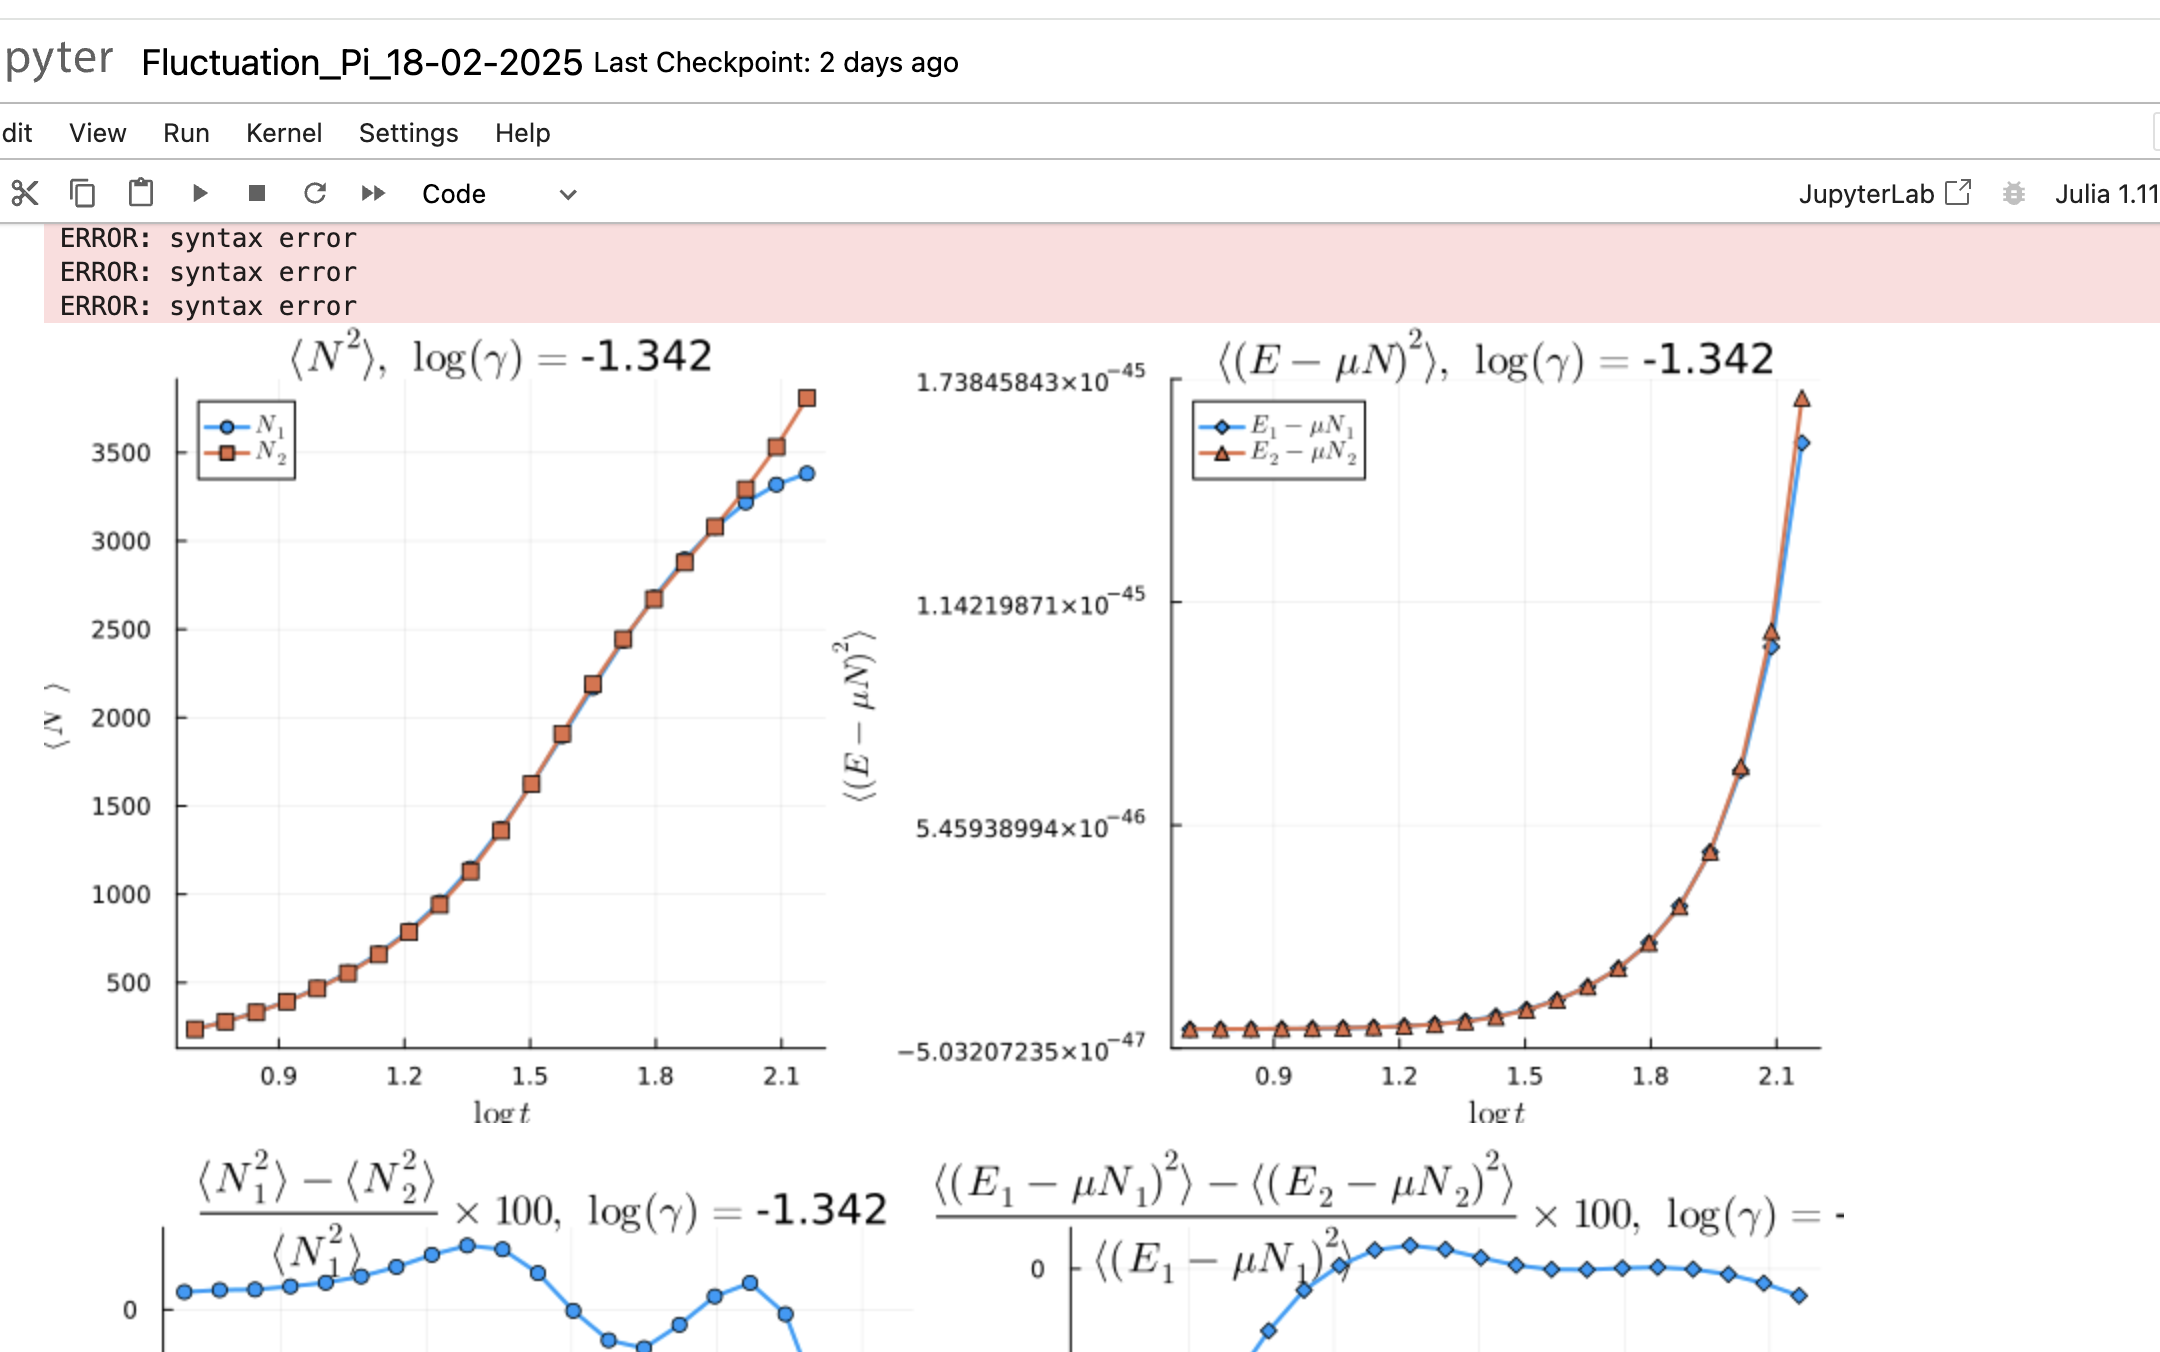
\includegraphics[width=1\textwidth]{Figures/test}

%\begin{aff}
%Donc une a l'ordre un en $\delta \theta (\operator{A}^{(0)})^{-1} %\operator{V}$ 

%\begin{eqnarray*}
%	\langle \delta \Pi ( \theta) \delta \Pi ( \theta') \rangle & = &  ( (\Pi^c_s - \Pi^c)\Pi^c/\Pi^c_s ) ( \theta ) \delta_{\theta, \theta'}/\delta \theta + \mathscr{F}(\theta , \theta' ) ,	
%\end{eqnarray*}

%avec 

%\begin{eqnarray*}
%	\mathscr{F}(\theta , \theta' ) & = & \left [ (\Pi^c_s - \Pi^c )( \theta)  +  (\Pi^c_s - \Pi^c ) ( \theta' )\right ] \frac{\Pi^c}{\Pi^c_s}(\theta)\frac{\Pi^c}{\Pi^c_s}(\theta') \frac{ \Delta( \theta'- \theta )}{ 2 \pi }\\
%	&&  - \left [ (\Pi^c_s - \Pi^c )( \theta)   (\Pi^c_s - \Pi^c ) ( \theta' )\right ] \frac{\Pi^c}{\Pi^c_s}(\theta)\frac{\Pi^c}{\Pi^c_s}(\theta')\int d\theta'' \left (   \frac{ \Pi^c/\Pi^c_s}{\Pi^c_s - \Pi^c} \right )(\theta'') \frac{\Delta(\theta''- \theta)}{2 \pi}\frac{\Delta(\theta''- \theta')}{2 \pi}  	
%\end{eqnarray*}
%\end{aff}



 













\subsection{Opérateurs conservés (intégrales du mouvement)}
%%Dans ce chapitre, nous nous intéressons aux fluctuations de la distribution de rapidité \( \delta \rho \) autour d'une distribution de référence \( \rho^c \), qui maximise la contribution à la fonction de partition des états, exprimée comme une fonctionnelle de la distribution \( \rho \) : 

La fonction de partition des états, s'exprime comme une fonctionnelle de la distribution \( \rho \) : 

\begin{eqnarray*}
	\Xi & = & \sum_\rho \exp \left( -\mathcal{A}(\rho) \right).
\end{eqnarray*}  

Dans la section {\em \bf Entropie de Yang-Yang} (\ref{??}), l'action \( \mathcal{A}(\rho) \) s'écrit sous la forme :  

\begin{eqnarray*}
	\mathcal{A}(\rho) & \doteq & - L\mathcal{S}_{YY}(\rho) + L\int f(\theta) \rho (\theta) \, d\theta,		
\end{eqnarray*}  

où \( \mathcal{S}_{YY} \) est la fonctionnelle d'entropie de Yang-Yang, définie dans (\ref{??}), et \( f \) est la fonction paramétrant les charges, introduite dans (\ref{??}).  

Dans cette même section {\em \bf Entropie de Yang-Yang} (\ref{??}), nous avons établi un lien entre \( f \) et distribution de référence \( \rho^c \), qui maximise la contribution à la fonction de partition des états .\\

On veux tester si nos experience est décrit pas un GGE. Pour cela nous nous intéressons aux fluctuations de la distribution de rapidité \( \delta \rho \) autour \( \rho^c \).

%Nous poursuivons à présent avec cette définition de l'action de classe $\mathcal{C}^2$ et admetant une distribution critique $\rho^c$ tel que sa différentielle en ce point critique soit nulle $d\mathcal{A}_{\rho^c} = 0 $ (\ref{??}) de sorte que d'aprés la formule de Taylor-Youg %afin de déterminer les fluctuations autour de \( \Pi^c \). Pour cela, nous réécrivons l'action sous la forme :  

Nous poursuivons à présent avec cette définition de l'action de classe $\mathcal{C}^2$ et admetant une distribution critique $\rho^c$ tel que sa différentielle en ce point critique soit nulle $d\mathcal{A}_{\rho^c} = 0 $ (\ref{??}) de sorte que d'aprés la formule de Taylor-Youg %afin de déterminer les fluctuations autour de \( \Pi^c \). Pour cela, nous réécrivons l'action sous la forme :  

\begin{eqnarray*}  
	\mathcal{A}(\rho^c + \delta \rho) & \underset{ \delta \rho \to 0 }{=} & \mathcal{A}(\rho^c)  + \frac{1}{2} \left. \frac{\delta^2 \mathcal{A}}{\delta \rho^2} \right|_{\rho^c} (\delta \rho) + \mathcal{O}((\delta \rho)^3),  
\end{eqnarray*}  

une expression quadratique pour l'action à l'ordre dominant en \( \delta \Pi \) avec $\left. \frac{\delta^2 \mathcal{A}}{\delta \rho^2} \right|_{\rho^c}$ la forme quadratique définie positive (Fig (\ref{fig.fluctu.A})).

\begin{figure}[H]
	\centering 
	\begin{tikzpicture}
		\begin{scope}[shift={(0,0)}]
			\begin{scope}[transform canvas={scale=0.6}]
				% Définition des couleurs avec les codes HTML
\definecolor{colorOne}{HTML}{443E46}
\definecolor{colorTwo}{HTML}{F6DEB8}
\definecolor{colorThree}{HTML}{908CA4}
\definecolor{colorFour}{HTML}{57659E}
\definecolor{colorFive}{HTML}{C57284}
\definecolor{colorSix}{HTML}{FF5B69}

% Raccourcis pour les couleurs
\def\colorOne{colorOne}
\def\colorTwo{colorTwo}
\def\colorThree{colorThree}
\def\colorFour{colorFour}
\def\colorFive{colorFive}
\def\colorSix{colorSix}

\def\colorslide{blue!50!black}



\begin{scope}
	% Tracer une courbe lisse entre des points
	\draw[shift={(0,0)} ,\colorOne]
		(-1 , 0 ) edge [thick,line width=0.8ex , ->,>=triangle 45  , \colorOne] node [pos = 1 , below ]{\huge$\rho$}( 5  , 0 )
	;
	\draw[shift={(0,0)}, color=\colorOne]
		(0, -1.0 ) edge [thick,line width=0.8ex , ->,>=triangle 45  ]node [pos=0.9,left=0.2cm ]{\huge$\mathcal{A}(\rho)$}( 0  , 5 )
	;
	\draw[]
		(2.5, 0.12 ) edge [thick,line width=0.8ex ,\colorThree ]node [pos=1,below  ]{\huge$\rho^c$} (2.5, -0.12 )	
	;
	
	\draw[]
		(2.5, -0.12 ) edge [thick,line width=0.4ex , dashed, \colorThree ] (2.5, 5.5 )
		(1.5, 1 ) edge [thick,line width=0.4ex , <->,>=triangle 45  , \colorThree ] (3.5, 1 )
		(-0.3,1) edge [thick,line width=0.4ex  , \colorThree ] node [pos=0,left ]{\huge$\mathcal{A}(\rho^c)$} (0.3, 1 )	
	;
    \draw[thick, line width=0.8ex , \colorFour] plot[smooth, tension=0.7] coordinates {
        (1, 5) (1.6 , 3 ) (2.5, 1) (3.5 , 3 )  (4, 5)
    };		
	
\end{scope}

	
			
			\end{scope}
			
			\draw[color = red , scale = 0.5 , draw = none  ] (-2 , -1) rectangle (5, 6) ; 	
		\end{scope}
		
		\begin{scope}[shift={(19,-1)}]
			\begin{scope}[transform canvas={scale=0.6}]
				% Définition des couleurs avec les codes HTML
\definecolor{colorOne}{HTML}{443E46}
\definecolor{colorTwo}{HTML}{F6DEB8}
\definecolor{colorThree}{HTML}{908CA4}
\definecolor{colorFour}{HTML}{57659E}
\definecolor{colorFive}{HTML}{C57284}
\definecolor{colorSix}{HTML}{FF5B69}

% Raccourcis pour les couleurs
\def\colorOne{colorOne}
\def\colorTwo{colorTwo}
\def\colorThree{colorThree}
\def\colorFour{colorFour}
\def\colorFive{colorFive}
\def\colorSix{colorSix}

\def\colorslide{blue!50!black}

\def\Occupation{
	\def\traitx{0.3}
	\def\traity{0.5}
	\draw[shift={(0,0)}]
		(-13.5 , 0 ) edge [thick,line width=0.8ex ]( -3.2  , 0 )
		( -3.2 - \traitx  , 0 - \traity ) edge [thick,line width=0.8ex ]( -3.2 + \traitx  , 0 + \traity  )
		( -2.8 - \traitx  , 0 - \traity ) edge [thick,line width=0.8ex ]( -2.8 + \traitx  , 0 + \traity  )
		(-2.8 , 0 ) edge [thick,line width=0.8ex ](2.8  , 0 )
		( 2.8 - \traitx  , 0 - \traity ) edge [thick,line width=0.8ex ]( 2.8 + \traitx  , 0 + \traity  )
		( 3.2 - \traitx  , 0 - \traity ) edge [thick,line width=0.8ex ]( 3.2 + \traitx  , 0 + \traity  )
		(3.2, 0 ) edge [thick,line width=0.8ex,->,>=triangle 45 , color = black ]node [pos=1.01,below  ]{\huge$\theta$}	( 13  , 0 )
	;
	\draw[shift={(0,0)}, color=\colorOne]
		(-10.5 , -1.5 ) edge [thick,line width=0.8ex , ->,>=triangle 45  ]( -10.5  , 4.5 )
	;
		
	\foreach \r in {1 , ... , 3 } {
%		\draw[
%		decoration={
%		markings,
%    	mark connection node=my node,
%    	mark=at position 0 with{\node [blue,transform shape] (my node) {\large \r};}},
%		color=gray, thick, 
%		line width=0.5ex] decorate { 
%            (-11.0, \r) -- (-10.1, \r )}
%        ;
        \draw[
			color=\colorOne,
			] 
            (-11.0, \r) edge[color=\colorThree , thick,line width=0.5ex] node [pos=-0.5 ]{\large\color{\colorFour} $\frac{\r}{\delta \theta}$ } (-10.3, \r )
        	;
	
	}
	

	
	% Graduation abcsisse 
	% Définitions des listes
% Definitions of the lists
\def\listetuple{-9/\theta_{1}, -8/\theta_{2} , -5/\theta_{3} , -2/\theta_{a-1} , 0/\theta_{a} , 1/\theta_{a+1} , 2/\theta_{a+2} ,  5/\theta_{N-4} , 7/\theta_{N-3},8/\theta_{N-1},9/\theta_{N} }
\def\listetrais{-12 , -11, -10, -9 , -8 , -7 ,  -6 , -5, -4.5,-4, -2 , -1, 0 , 0.5, 1, 2, 4 , 5 ,  6 , 7 , 8 ,8.5, 9 ,  10 , 11, 12 }

% Loop over listetrais
\foreach \r in \listetrais {
    % Initialize found variable to zero
    % Initialize found variable to zero
    %\pgfmathsetmacro\found{0}
    \global\def\found{0}
    \xdef\nomtheta{}
    
    % Check if \r is in listetuple
    \foreach \x/\y in \listetuple { 
        \ifdim \r pt=\x pt % If \r matches any \x in listetuple
            \global\def\found{1} ;
            \xdef\nomtheta{\y} % Set \nomtheta to the corresponding \y
            %\pgfmathsetmacro\found{1} % Set found to 1            
            %\global\pgfmathsetmacro\found{1}
        \fi
    }
    
    %\node [circle, draw, red] (A) at (\r, 2) {\found , $\nomtheta$};
    
    % Draw the line and display \nomtheta if found
    \ifnum\found=1
        \draw[color=\colorOne, thick, line width=0.5ex] 
            (\r, -0.3) -- (\r, 0.3) node[red , pos=-0.5] {\large $\nomtheta$};
         \filldraw[line width=0.5ex, color=\colorSix, outer color=\colorSix, inner color=\colorSix] 
            (\r, 0) circle (4pt);
    \else 
        % Draw without \nomtheta and add a blue circle if not found
        \draw[color=\colorOne, thick, line width=0.5ex] 
            (\r, -0.3) -- (\r, 0.3);
        \filldraw[line width=0.5ex, color=\colorSix, outer color=\colorTwo, inner color=\colorTwo] 
            (\r, 0) circle (4pt); 
    \fi
}

\def\listetrais{-9.5/\theta_{i-1}/2/3, -6.5/\theta_{i}/1/4  ,   -1.5/\theta_{j}/2/4 , 1.5/\theta_{j+1}/-1/3 , 3.5/\theta_{\ell-1}/1/3 , 6.5/\theta_{\ell}/3/4 , 9.5/\theta(\theta_{\ell+1})/-1/3 };



\foreach \r/\nomx/\y/\ys in \listetrais {
	\draw[
		decoration={
		markings,
    	mark connection node=my node,
    	mark=at position .5 with{\node [blue,transform shape] (my node) {\large \color{\colorFour} $\nomx$};}},
		color=\colorThree , thick, 
		line width=0.5ex] decorate { 
            (\r, 0.12) -- (\r, -1.2)}
        ;
     
     \ifdim \y pt > -1 pt 
     	\draw[
			decoration={
			markings,
    		mark connection node=my node,
    		mark=at position .5 with{\node [blue,transform shape] (my node) {\large \color{\colorFour} $\Pi(\nomx) $};}},
			color=\colorThree, thick, 
			line width=0.5ex] decorate { 
            (\r, \y) -- (\r +3, \y)}
        ;
        \draw[
			decoration={
			markings,
    		mark connection node=my node,
    		mark=at position .5 with{\node [blue,transform shape] (my node) {\large \color{\colorFive} $\Pi_s(\nomx) $};}},
			color=\colorFive, thick, 
			line width=0.5ex] decorate { 
            (\r, \ys) -- (\r +3, \ys)}
        ;
     \fi 
     \ifdim \r pt= -1.5 pt
     	\draw[
     		decoration={
			markings,
    		mark connection node=my node,
    		mark=at position .5 with{\node [blue,transform shape] (my node) {\large \color{\colorFour}  $\delta \theta $};},
    		%mark=at position 0.1  with {\arrow[blue, line width=0.5ex]{<}},
    		%mark=at position 1  with {\arrow[blue, line width=0.5ex]{>}}
    		},
        	color=\colorThree,
        	thick,
        	line width=0.5ex,
        	%arrows={Computer Modern Rightarrow[line cap=round]-Computer Modern Rightarrow[line cap=round]}
   			](\r, -1.2) edge[arrows={Computer Modern Rightarrow[line cap=round]-}] (\r + 0.4, -1.2)decorate {
    		(\r, -1.2) -- (\r + 3, -1.2)}(\r + 2, -1.2) edge[arrows={-Computer Modern Rightarrow[line cap=round]}] (\r + 3, -1.2)
    		;
    \fi
			
	
}


			
}


\begin{scope}
	%\draw[help lines , width=1.5ex] (-8,-3) grid (8,3);\draw[help lines ,width=0.5ex , opacity = 0.5] (-3,-3) grid[step=0.1] (3,3));
	
	%\draw[help lines] 
	%	(-3,-3) edge[width=1.5ex] grid (3,3)	
	%	(-3,-3) edge[width=0.5ex , opacity = 0.5] grid (3,3)	
	%;
	\begin{scope}[shift={(0,1)},rotate=0,opacity=1,color=black]
		\Occupation	
		
		%\node[anchor=east, font=\bfseries] at (-11, 0) {\color{red}\large (T = 0 )} ;	
	\end{scope}
	
	
	
	
	\begin{scope}[shift={(-10.5,7)},rotate=0,opacity=1,color=black]
	
	\begin{scope}[shift={(-0,0)},rotate=0,opacity=1,color=black]
	
		\draw[shift={(0,0)} ,line width=1ex,rounded corners = 1ex,color=\colorOne , opacity =1 ,fill=\colorOne!00 , pattern={north east lines} , pattern color=\colorOne!00 ]
			(0 , -1 ) rectangle (5,1)
		;
		

		\begin{scope}[shift={(0.5,0.5)}]
			\draw[color=\colorOne, thick, line width=0.5ex] 
            (0, -0.3) -- (0, 0.3) ;
            \filldraw[line width=0.5ex, color=\colorSix, outer color=\colorSix, inner color=\colorSix] 
            (0, 0) circle (4pt);
            
            \node[anchor=west, font=\bfseries] at (0.2, 0) {\color{\colorSix}\large : quasi-particule};
		\end{scope}
		
		\begin{scope}[shift={(0.5,-0.5)}]
			\draw[color=\colorOne, thick, line width=0.5ex] 
            (0, -0.3) -- (0, 0.3) ;
            \filldraw[line width=0.5ex, color=\colorSix, outer color=\colorTwo, inner color=\colorTwo] 
            (0, 0) circle (4pt);
            
            \node[anchor=west, font=\bfseries] at (0.2, 0) {\color{\colorSix}\large : hole};
		\end{scope}

	\end{scope}
	
	\begin{scope}[shift={(6,0)},rotate=0,opacity=1,color=black]	
		
		\draw[shift={(0,0)} ,line width=1ex,rounded corners = 1ex,color=\colorOne , opacity =1 ,fill=\colorOne!00 , pattern={north east lines} , pattern color=\colorOne!00 ]
			(0 , -1 ) rectangle (7.5,1)
		;
		
		\node[anchor=west] at (0.5, 0.5) {\color{\colorFour}\large $\Pi$ };\node[anchor=west, font=\bfseries] at (1, 0.5) {\color{\colorFour}\large : quasi-particule distribution};
		
		\node[anchor=west] at (0.5, -0.5) {\color{\colorFour}\large $\Pi_h$ };\node[anchor=west, font=\bfseries] at (1, -0.5) {\color{\colorFour}\large  : hole distribution};
		
	\end{scope}
	
	\begin{scope}[shift={(14.5,0)},rotate=0,opacity=1,color=black]	
		
		\draw[shift={(0,0)} ,line width=1ex,rounded corners = 1ex,color=\colorOne , opacity =1 ,fill=\colorOne!00 , pattern={north east lines} , pattern color=\colorOne!00 ]
			(0 , -0.5 ) rectangle (7.0,0.5)
		;
		
		\node[anchor=west] at (0.2, 0) {\color{\colorFour}\large ${\color{\colorFive}\Pi_s} = \Pi + \Pi_h $ } node[anchor=west , font=\bfseries] at (3.1 , 0 )  {\color{\colorFour}\large {\color{\colorFive} : density of states}};
		
	\end{scope}
	
	
	\end{scope}


		
	
\end{scope}

	
			
			\end{scope}
			\begin{scope}[scale=1]
				\draw[color = red , scale = 1 , draw = none  ] (-1 , -1) rectangle (5, 5) ; 
			\end{scope}	
		\end{scope}

		
				
			
	\end{tikzpicture}	
	\captionsetup{skip=10pt} % Ajoute de l’espace après la légende
	\label{fig.fluctu.A}
\end{figure}


On discrétise l'axe des rapidités en  petite cellule de rapidité $[\theta, \theta+\delta\theta]$, qui contient $L\rho(\theta) \delta \theta$ rapidités. 
	



Avec ces petites tranches, la forme quadratique s’écrit :

\begin{eqnarray*}
    \left. \frac{\delta^2 \mathcal{A}}{{\delta \rho}^2} \right|_{\rho^c}(\delta \rho ) &=&  \sum_{a,b \mid \text{tranche}}  
    \delta \rho(\theta_a)  \frac{\partial^2 \mathcal{A}}{\partial \delta \rho(\theta_a) \partial \delta \rho(\theta_b) } (\rho^c)  \delta \rho(\theta_b).
\end{eqnarray*}
Les fluctuations s’écrivent donc :

\begin{eqnarray*}
    \langle \delta \rho ( \theta) \delta \rho ( \theta') \rangle &=&  
    \frac{ \int d\delta \rho \, \delta \rho(\theta) \delta \rho ( \theta') 
    \exp \left( - \frac{1}{2} \sum_{a,b \mid \text{tranche}}  
    \delta \rho(\theta_a) \frac{\partial^2 \mathcal{A}}{\partial \delta \rho(\theta_a) \partial \delta \rho(\theta_b) } (\rho^c)  \delta \rho(\theta_b) \right) }
    { \int d\delta \Pi  
    \exp \left( - \frac{1}{2} \sum_{a,b \mid \text{tranche}}  
    \delta \rho(\theta_a) \frac{\partial^2 \mathcal{A}}{\partial \delta \rho(\theta_a) \partial \delta \rho(\theta_b) } (\rho^c)  \delta \rho(\theta_b) \right) } \\
    &=& \left( \mathbf{A}^{-1} \right)_{\theta , \theta'}
\end{eqnarray*}


\begin{aff}

\begin{eqnarray*}
	\langle \delta \rho ( \theta) \delta \rho ( \theta') \rangle &=& 	\left( \mathbf{A}^{-1} \right)_{\theta , \theta'}
\end{eqnarray*}

	
avec la  {\em matrice hessienne} $\mathbf{A}_{\theta , \theta'} \equiv \frac{\partial^2 \mathcal{A}}{\partial \delta \rho(\theta) \partial \delta \rho(\theta') }(\rho^c)$, au point critique/ qui maximise la probabilité  $\rho^c=\rho^c_s \nu^c $, s'écrit

\begin{eqnarray*}
	\operator{A} & = & \operator{A}^{(0)} + \delta \theta \operator{V}
\end{eqnarray*}

avec 

\begin{eqnarray*}
	A^{(0)}_{\theta , \theta'}  & = &  L\delta \theta \left ( \frac{ 1}{\rho^c_s ( 1  - \nu^c ) \nu^c } \right )(\theta)    \delta({\theta - \theta '})	,\\
	V_{\theta , \theta'}  &= & L \delta \theta \left \{ - \left [ \left ( \frac{1}{\rho^c_s( 1 - \nu^c) } \right ) ( \theta)  +  \left ( \frac{1}{\rho^c_s( 1 - \nu^c) } \right ) ( \theta' )\right ] \frac{ \Delta( \theta'- \theta )}{ 2 \pi } + \int d\theta''  \left ( \frac{\nu^c}{\rho^c_s( 1 - \nu^c) } \right )(\theta'') \frac{\Delta(\theta''- \theta)}{2 \pi}\frac{\Delta(\theta''- \theta')}{2 \pi}   \right \} 	
\end{eqnarray*}

\end{aff}

\subsection{Testes}

\begin{eqnarray*}
	\Delta_{\operator{\mathcal{N}}}^2  & = &  \frac{1}{\beta} \left . \frac{\partial \langle \operator{\mathcal{N}} \rangle}{\partial \mu} \right )_T \\
	\Delta_{\operator{\mathcal{E}}-\mu \operator{\mathcal{N}}}^2  & = &  - \left . \frac{\partial \langle \operator{\mathcal{E}}-\mu \operator{\mathcal{N}} \rangle}{\partial \beta} \right )_\mu 
\end{eqnarray*}

et 

\begin{eqnarray*}
	\Delta_{\operator{\mathcal{N}}}^2  &= & L^2 \int d\theta_a \int d \theta_b \, \langle \delta \rho(\theta_a) \delta \rho(\theta_b) \rangle \\
	\Delta_{\operator{\mathcal{E}}-\mu \operator{\mathcal{N}}}^2  & = & L^2 \int d\theta_a \int d \theta_b \, \left ( - \mu + \frac{1}2 m \theta_a^2  \right  )\left ( - \mu + \frac{1}2 m \theta_b^2  \right  )  \langle \delta \rho(\theta_a) \delta \rho(\theta_b) \rangle
\end{eqnarray*}

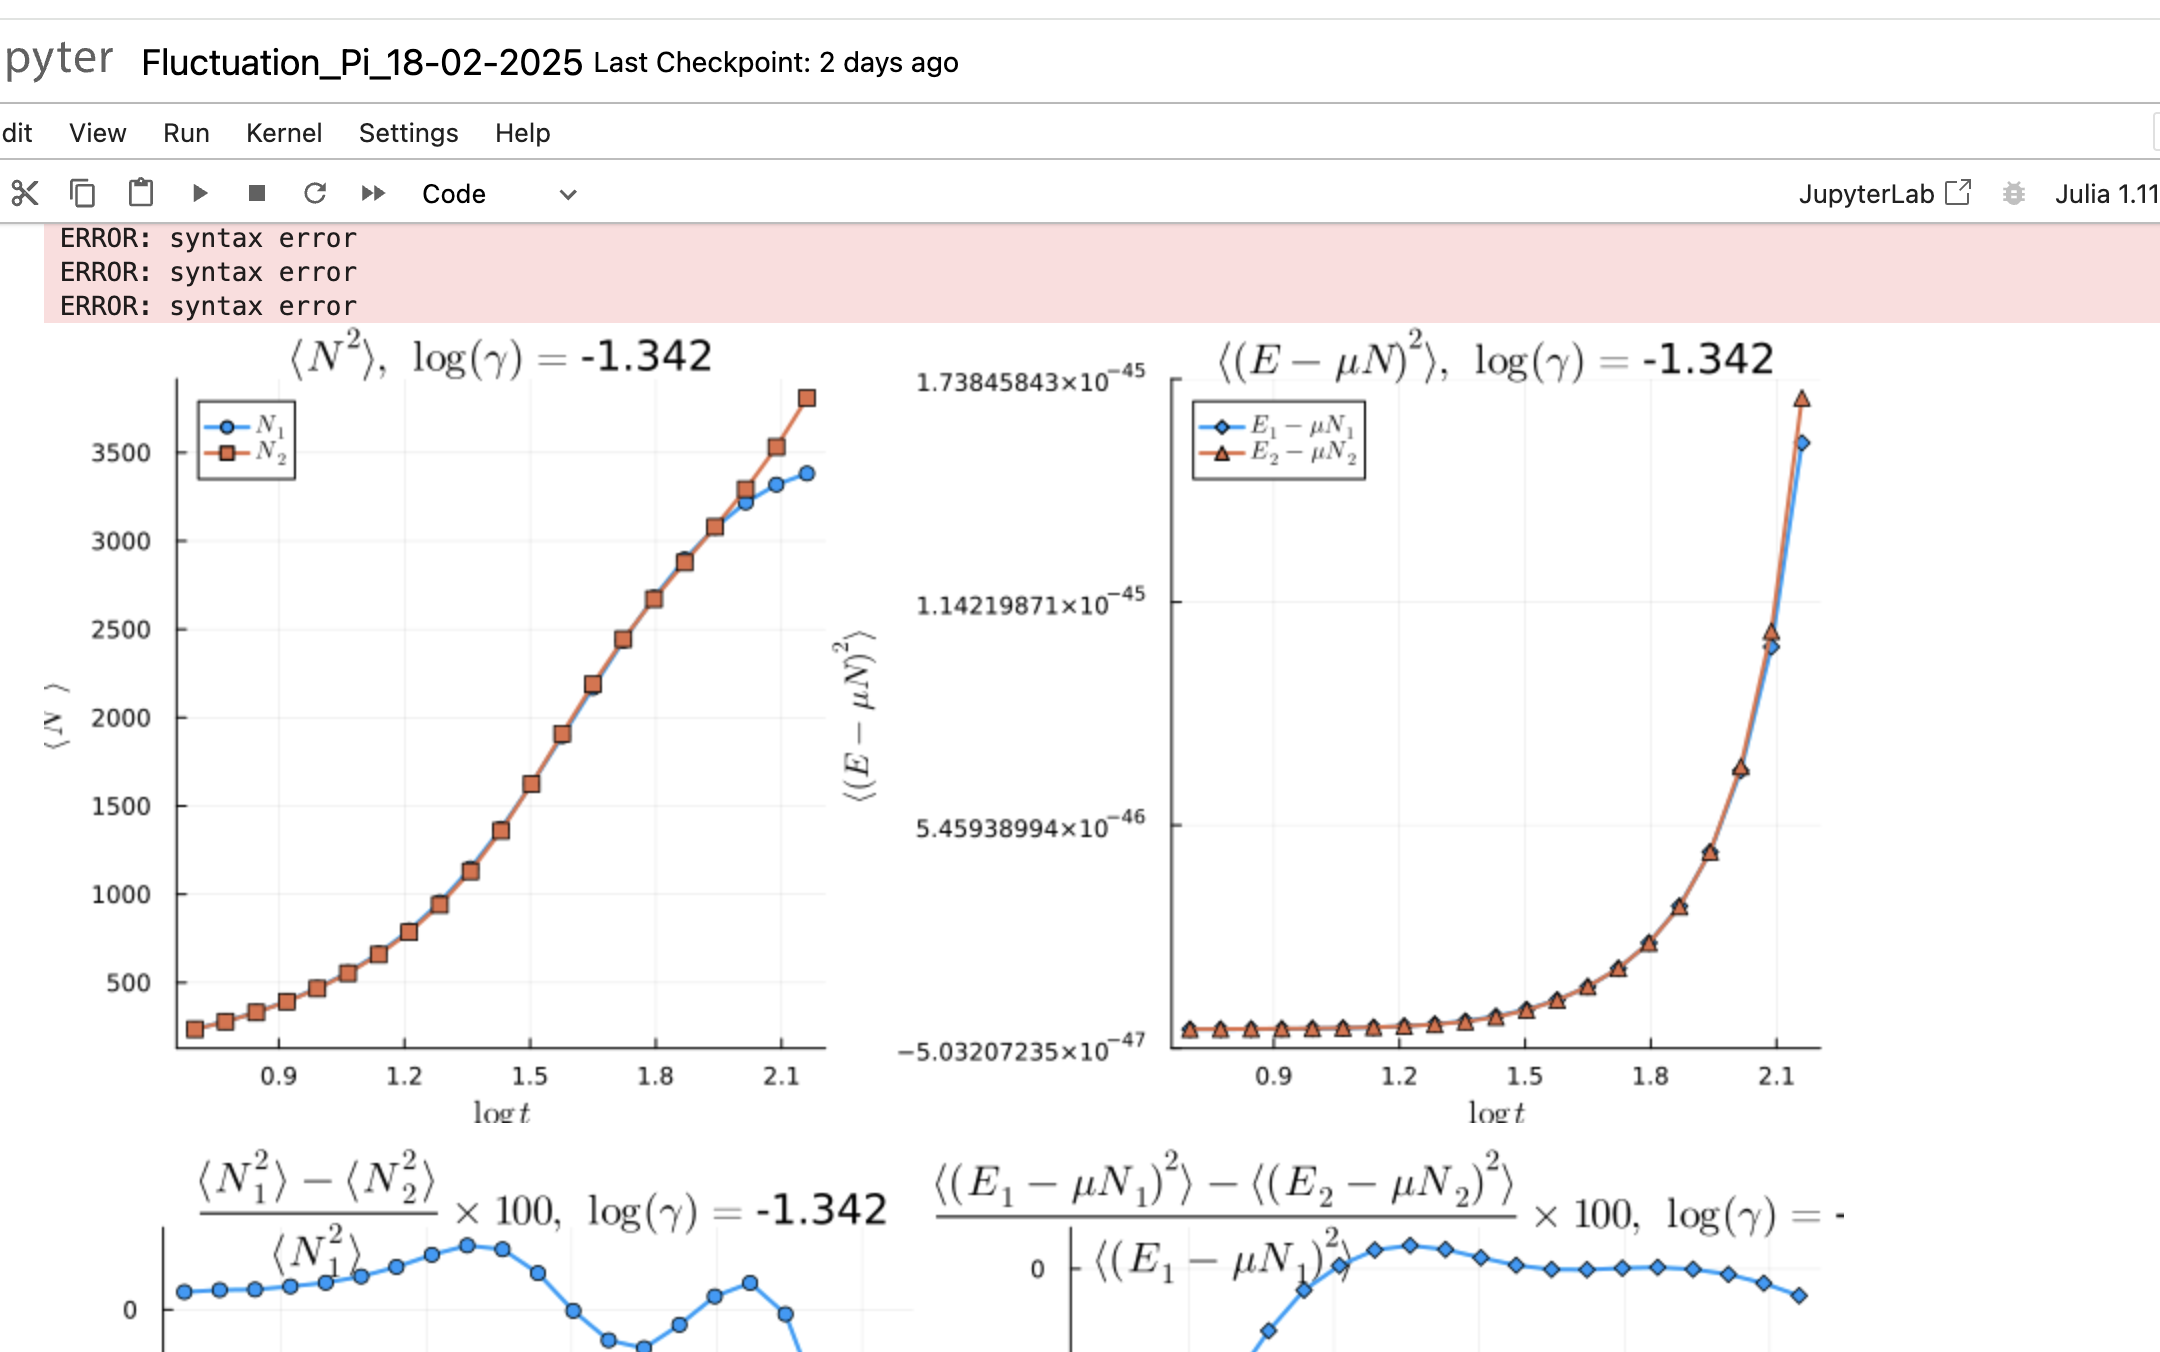
\includegraphics[width=1\textwidth]{Figures/test}

%\begin{aff}
%Donc une a l'ordre un en $\delta \theta (\operator{A}^{(0)})^{-1} %\operator{V}$ 

%\begin{eqnarray*}
%	\langle \delta \Pi ( \theta) \delta \Pi ( \theta') \rangle & = &  ( (\Pi^c_s - \Pi^c)\Pi^c/\Pi^c_s ) ( \theta ) \delta_{\theta, \theta'}/\delta \theta + \mathscr{F}(\theta , \theta' ) ,	
%\end{eqnarray*}

%avec 

%\begin{eqnarray*}
%	\mathscr{F}(\theta , \theta' ) & = & \left [ (\Pi^c_s - \Pi^c )( \theta)  +  (\Pi^c_s - \Pi^c ) ( \theta' )\right ] \frac{\Pi^c}{\Pi^c_s}(\theta)\frac{\Pi^c}{\Pi^c_s}(\theta') \frac{ \Delta( \theta'- \theta )}{ 2 \pi }\\
%	&&  - \left [ (\Pi^c_s - \Pi^c )( \theta)   (\Pi^c_s - \Pi^c ) ( \theta' )\right ] \frac{\Pi^c}{\Pi^c_s}(\theta)\frac{\Pi^c}{\Pi^c_s}(\theta')\int d\theta'' \left (   \frac{ \Pi^c/\Pi^c_s}{\Pi^c_s - \Pi^c} \right )(\theta'') \frac{\Delta(\theta''- \theta)}{2 \pi}\frac{\Delta(\theta''- \theta')}{2 \pi}  	
%\end{eqnarray*}
%\end{aff}



 








\subsection{Introduction au modèle de gaz de Bose unidimensionnel}
%Dans ce chapitre, nous nous intéressons aux fluctuations de la distribution de rapidité \( \delta \rho \) autour d'une distribution de référence \( \rho^c \), qui maximise la contribution à la fonction de partition des états, exprimée comme une fonctionnelle de la distribution \( \rho \) : 

La fonction de partition des états, s'exprime comme une fonctionnelle de la distribution \( \rho \) : 

\begin{eqnarray*}
	\Xi & = & \sum_\rho \exp \left( -\mathcal{A}(\rho) \right).
\end{eqnarray*}  

Dans la section {\em \bf Entropie de Yang-Yang} (\ref{??}), l'action \( \mathcal{A}(\rho) \) s'écrit sous la forme :  

\begin{eqnarray*}
	\mathcal{A}(\rho) & \doteq & - L\mathcal{S}_{YY}(\rho) + L\int f(\theta) \rho (\theta) \, d\theta,		
\end{eqnarray*}  

où \( \mathcal{S}_{YY} \) est la fonctionnelle d'entropie de Yang-Yang, définie dans (\ref{??}), et \( f \) est la fonction paramétrant les charges, introduite dans (\ref{??}).  

Dans cette même section {\em \bf Entropie de Yang-Yang} (\ref{??}), nous avons établi un lien entre \( f \) et distribution de référence \( \rho^c \), qui maximise la contribution à la fonction de partition des états .\\

On veux tester si nos experience est décrit pas un GGE. Pour cela nous nous intéressons aux fluctuations de la distribution de rapidité \( \delta \rho \) autour \( \rho^c \).

%Nous poursuivons à présent avec cette définition de l'action de classe $\mathcal{C}^2$ et admetant une distribution critique $\rho^c$ tel que sa différentielle en ce point critique soit nulle $d\mathcal{A}_{\rho^c} = 0 $ (\ref{??}) de sorte que d'aprés la formule de Taylor-Youg %afin de déterminer les fluctuations autour de \( \Pi^c \). Pour cela, nous réécrivons l'action sous la forme :  

Nous poursuivons à présent avec cette définition de l'action de classe $\mathcal{C}^2$ et admetant une distribution critique $\rho^c$ tel que sa différentielle en ce point critique soit nulle $d\mathcal{A}_{\rho^c} = 0 $ (\ref{??}) de sorte que d'aprés la formule de Taylor-Youg %afin de déterminer les fluctuations autour de \( \Pi^c \). Pour cela, nous réécrivons l'action sous la forme :  

\begin{eqnarray*}  
	\mathcal{A}(\rho^c + \delta \rho) & \underset{ \delta \rho \to 0 }{=} & \mathcal{A}(\rho^c)  + \frac{1}{2} \left. \frac{\delta^2 \mathcal{A}}{\delta \rho^2} \right|_{\rho^c} (\delta \rho) + \mathcal{O}((\delta \rho)^3),  
\end{eqnarray*}  

une expression quadratique pour l'action à l'ordre dominant en \( \delta \Pi \) avec $\left. \frac{\delta^2 \mathcal{A}}{\delta \rho^2} \right|_{\rho^c}$ la forme quadratique définie positive (Fig (\ref{fig.fluctu.A})).

\begin{figure}[H]
	\centering 
	\begin{tikzpicture}
		\begin{scope}[shift={(0,0)}]
			\begin{scope}[transform canvas={scale=0.6}]
				\input{Figures/Fonc_A_code}	
			
			\end{scope}
			
			\draw[color = red , scale = 0.5 , draw = none  ] (-2 , -1) rectangle (5, 6) ; 	
		\end{scope}
		
		\begin{scope}[shift={(19,-1)}]
			\begin{scope}[transform canvas={scale=0.6}]
				\input{Figures/Occupation_theta_code}	
			
			\end{scope}
			\begin{scope}[scale=1]
				\draw[color = red , scale = 1 , draw = none  ] (-1 , -1) rectangle (5, 5) ; 
			\end{scope}	
		\end{scope}

		
				
			
	\end{tikzpicture}	
	\captionsetup{skip=10pt} % Ajoute de l’espace après la légende
	\label{fig.fluctu.A}
\end{figure}


On discrétise l'axe des rapidités en  petite cellule de rapidité $[\theta, \theta+\delta\theta]$, qui contient $L\rho(\theta) \delta \theta$ rapidités. 
	



Avec ces petites tranches, la forme quadratique s’écrit :

\begin{eqnarray*}
    \left. \frac{\delta^2 \mathcal{A}}{{\delta \rho}^2} \right|_{\rho^c}(\delta \rho ) &=&  \sum_{a,b \mid \text{tranche}}  
    \delta \rho(\theta_a)  \frac{\partial^2 \mathcal{A}}{\partial \delta \rho(\theta_a) \partial \delta \rho(\theta_b) } (\rho^c)  \delta \rho(\theta_b).
\end{eqnarray*}
Les fluctuations s’écrivent donc :

\begin{eqnarray*}
    \langle \delta \rho ( \theta) \delta \rho ( \theta') \rangle &=&  
    \frac{ \int d\delta \rho \, \delta \rho(\theta) \delta \rho ( \theta') 
    \exp \left( - \frac{1}{2} \sum_{a,b \mid \text{tranche}}  
    \delta \rho(\theta_a) \frac{\partial^2 \mathcal{A}}{\partial \delta \rho(\theta_a) \partial \delta \rho(\theta_b) } (\rho^c)  \delta \rho(\theta_b) \right) }
    { \int d\delta \Pi  
    \exp \left( - \frac{1}{2} \sum_{a,b \mid \text{tranche}}  
    \delta \rho(\theta_a) \frac{\partial^2 \mathcal{A}}{\partial \delta \rho(\theta_a) \partial \delta \rho(\theta_b) } (\rho^c)  \delta \rho(\theta_b) \right) } \\
    &=& \left( \mathbf{A}^{-1} \right)_{\theta , \theta'}
\end{eqnarray*}


\begin{aff}

\begin{eqnarray*}
	\langle \delta \rho ( \theta) \delta \rho ( \theta') \rangle &=& 	\left( \mathbf{A}^{-1} \right)_{\theta , \theta'}
\end{eqnarray*}

	
avec la  {\em matrice hessienne} $\mathbf{A}_{\theta , \theta'} \equiv \frac{\partial^2 \mathcal{A}}{\partial \delta \rho(\theta) \partial \delta \rho(\theta') }(\rho^c)$, au point critique/ qui maximise la probabilité  $\rho^c=\rho^c_s \nu^c $, s'écrit

\begin{eqnarray*}
	\operator{A} & = & \operator{A}^{(0)} + \delta \theta \operator{V}
\end{eqnarray*}

avec 

\begin{eqnarray*}
	A^{(0)}_{\theta , \theta'}  & = &  L\delta \theta \left ( \frac{ 1}{\rho^c_s ( 1  - \nu^c ) \nu^c } \right )(\theta)    \delta({\theta - \theta '})	,\\
	V_{\theta , \theta'}  &= & L \delta \theta \left \{ - \left [ \left ( \frac{1}{\rho^c_s( 1 - \nu^c) } \right ) ( \theta)  +  \left ( \frac{1}{\rho^c_s( 1 - \nu^c) } \right ) ( \theta' )\right ] \frac{ \Delta( \theta'- \theta )}{ 2 \pi } + \int d\theta''  \left ( \frac{\nu^c}{\rho^c_s( 1 - \nu^c) } \right )(\theta'') \frac{\Delta(\theta''- \theta)}{2 \pi}\frac{\Delta(\theta''- \theta')}{2 \pi}   \right \} 	
\end{eqnarray*}

\end{aff}

\subsection{Testes}

\begin{eqnarray*}
	\Delta_{\operator{\mathcal{N}}}^2  & = &  \frac{1}{\beta} \left . \frac{\partial \langle \operator{\mathcal{N}} \rangle}{\partial \mu} \right )_T \\
	\Delta_{\operator{\mathcal{E}}-\mu \operator{\mathcal{N}}}^2  & = &  - \left . \frac{\partial \langle \operator{\mathcal{E}}-\mu \operator{\mathcal{N}} \rangle}{\partial \beta} \right )_\mu 
\end{eqnarray*}

et 

\begin{eqnarray*}
	\Delta_{\operator{\mathcal{N}}}^2  &= & L^2 \int d\theta_a \int d \theta_b \, \langle \delta \rho(\theta_a) \delta \rho(\theta_b) \rangle \\
	\Delta_{\operator{\mathcal{E}}-\mu \operator{\mathcal{N}}}^2  & = & L^2 \int d\theta_a \int d \theta_b \, \left ( - \mu + \frac{1}2 m \theta_a^2  \right  )\left ( - \mu + \frac{1}2 m \theta_b^2  \right  )  \langle \delta \rho(\theta_a) \delta \rho(\theta_b) \rangle
\end{eqnarray*}

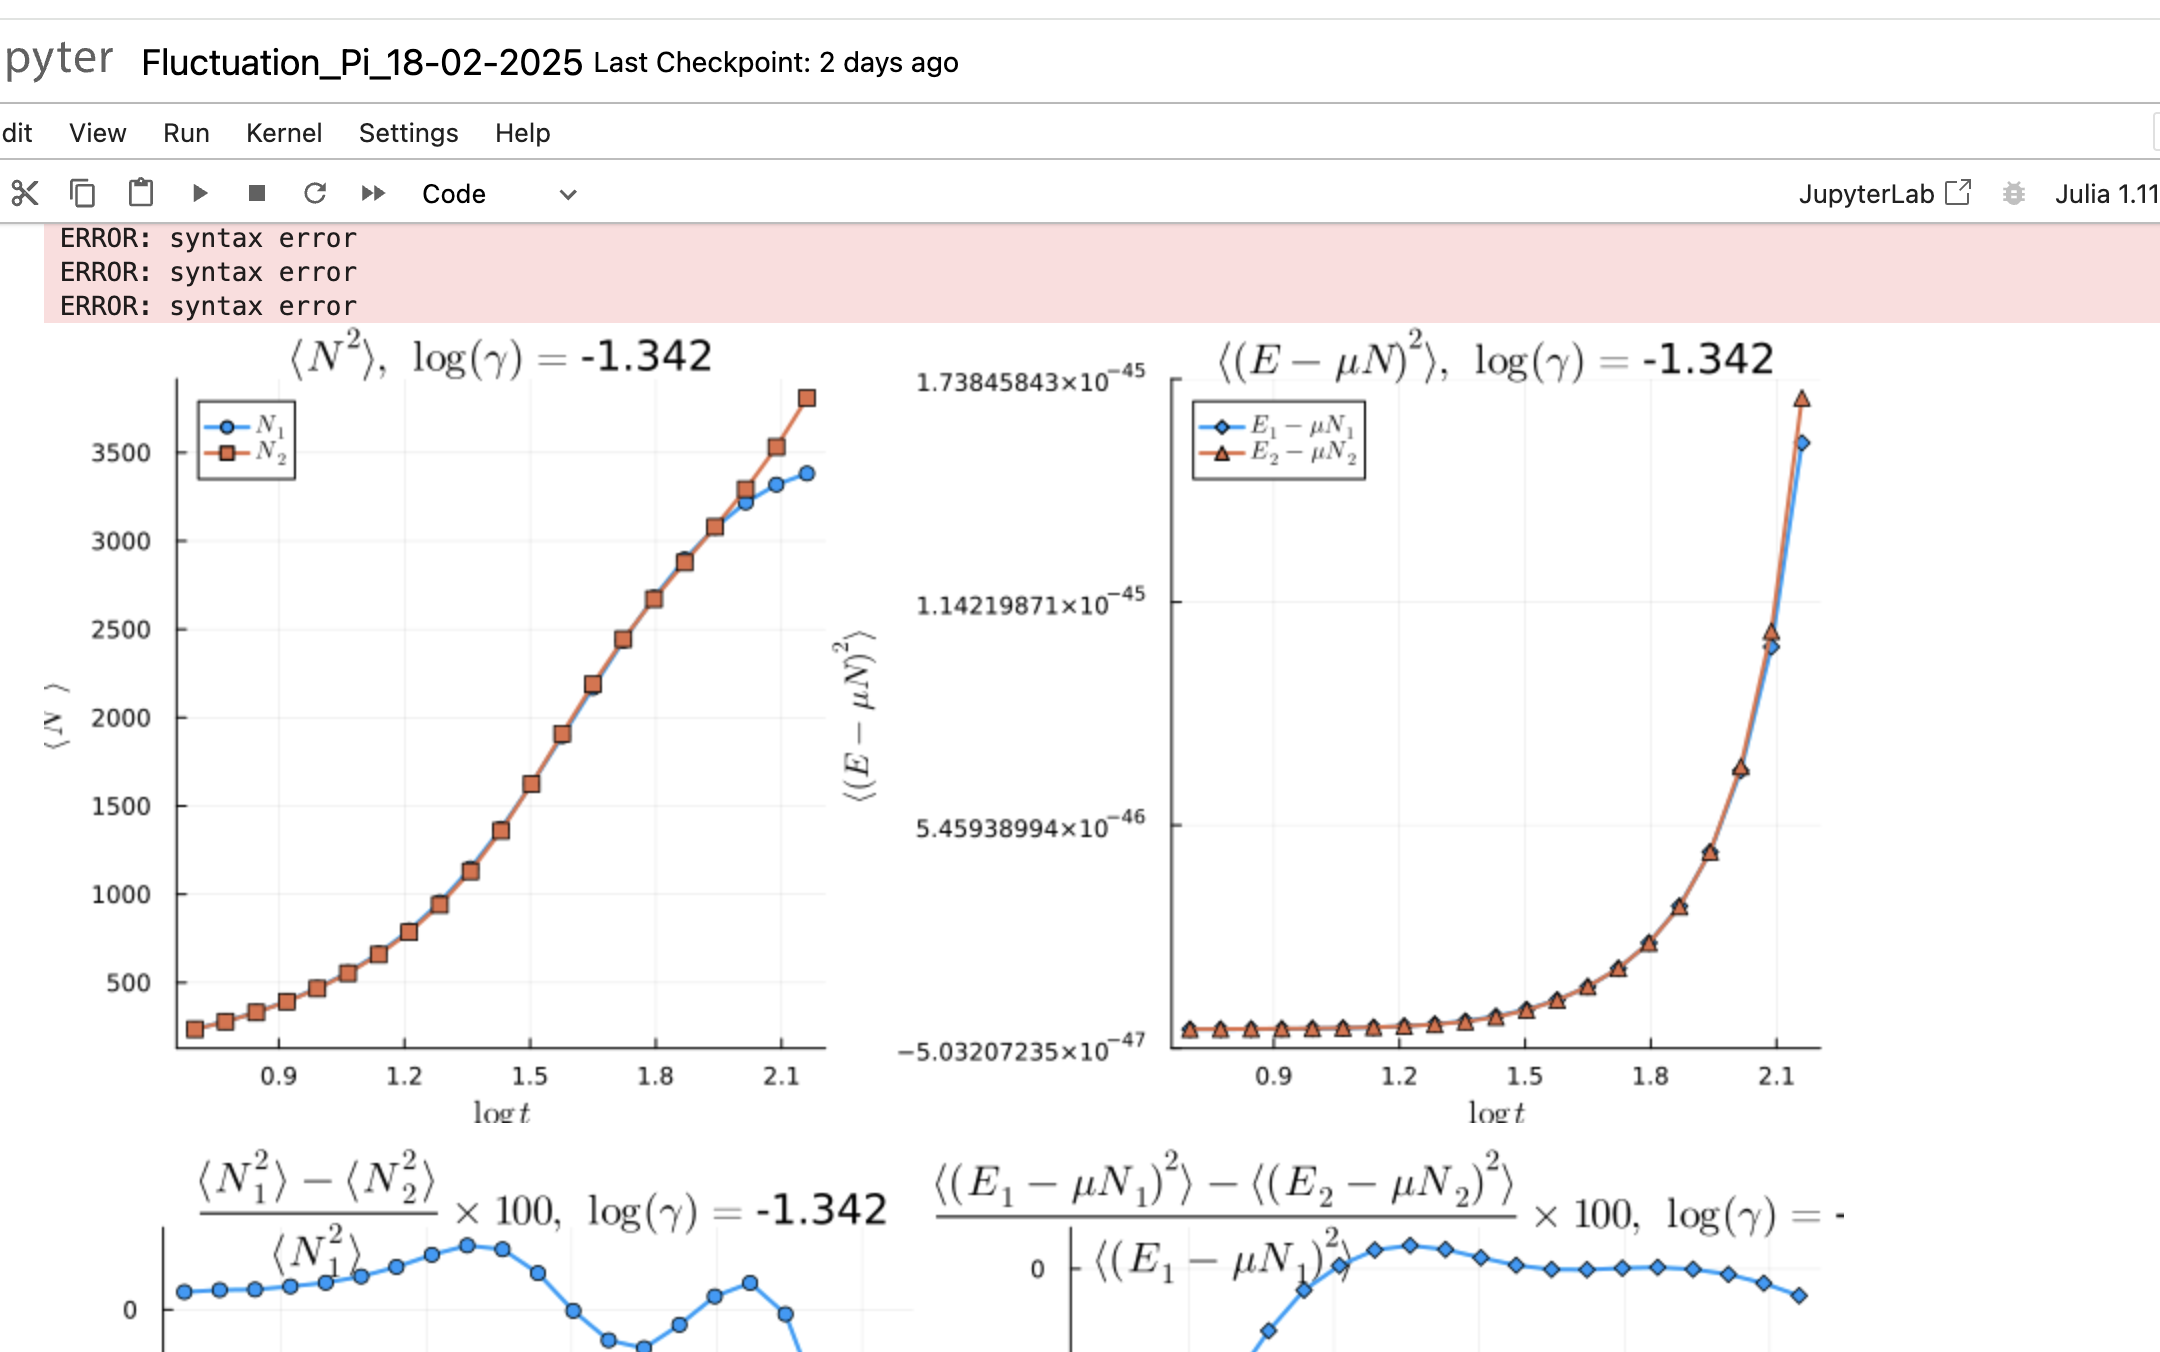
\includegraphics[width=1\textwidth]{Figures/test}

%\begin{aff}
%Donc une a l'ordre un en $\delta \theta (\operator{A}^{(0)})^{-1} %\operator{V}$ 

%\begin{eqnarray*}
%	\langle \delta \Pi ( \theta) \delta \Pi ( \theta') \rangle & = &  ( (\Pi^c_s - \Pi^c)\Pi^c/\Pi^c_s ) ( \theta ) \delta_{\theta, \theta'}/\delta \theta + \mathscr{F}(\theta , \theta' ) ,	
%\end{eqnarray*}

%avec 

%\begin{eqnarray*}
%	\mathscr{F}(\theta , \theta' ) & = & \left [ (\Pi^c_s - \Pi^c )( \theta)  +  (\Pi^c_s - \Pi^c ) ( \theta' )\right ] \frac{\Pi^c}{\Pi^c_s}(\theta)\frac{\Pi^c}{\Pi^c_s}(\theta') \frac{ \Delta( \theta'- \theta )}{ 2 \pi }\\
%	&&  - \left [ (\Pi^c_s - \Pi^c )( \theta)   (\Pi^c_s - \Pi^c ) ( \theta' )\right ] \frac{\Pi^c}{\Pi^c_s}(\theta)\frac{\Pi^c}{\Pi^c_s}(\theta')\int d\theta'' \left (   \frac{ \Pi^c/\Pi^c_s}{\Pi^c_s - \Pi^c} \right )(\theta'') \frac{\Delta(\theta''- \theta)}{2 \pi}\frac{\Delta(\theta''- \theta')}{2 \pi}  	
%\end{eqnarray*}
%\end{aff}



 









\subsection{Hamiltonien du modèle}
%Dans ce chapitre, nous nous intéressons aux fluctuations de la distribution de rapidité \( \delta \rho \) autour d'une distribution de référence \( \rho^c \), qui maximise la contribution à la fonction de partition des états, exprimée comme une fonctionnelle de la distribution \( \rho \) : 

La fonction de partition des états, s'exprime comme une fonctionnelle de la distribution \( \rho \) : 

\begin{eqnarray*}
	\Xi & = & \sum_\rho \exp \left( -\mathcal{A}(\rho) \right).
\end{eqnarray*}  

Dans la section {\em \bf Entropie de Yang-Yang} (\ref{??}), l'action \( \mathcal{A}(\rho) \) s'écrit sous la forme :  

\begin{eqnarray*}
	\mathcal{A}(\rho) & \doteq & - L\mathcal{S}_{YY}(\rho) + L\int f(\theta) \rho (\theta) \, d\theta,		
\end{eqnarray*}  

où \( \mathcal{S}_{YY} \) est la fonctionnelle d'entropie de Yang-Yang, définie dans (\ref{??}), et \( f \) est la fonction paramétrant les charges, introduite dans (\ref{??}).  

Dans cette même section {\em \bf Entropie de Yang-Yang} (\ref{??}), nous avons établi un lien entre \( f \) et distribution de référence \( \rho^c \), qui maximise la contribution à la fonction de partition des états .\\

On veux tester si nos experience est décrit pas un GGE. Pour cela nous nous intéressons aux fluctuations de la distribution de rapidité \( \delta \rho \) autour \( \rho^c \).

%Nous poursuivons à présent avec cette définition de l'action de classe $\mathcal{C}^2$ et admetant une distribution critique $\rho^c$ tel que sa différentielle en ce point critique soit nulle $d\mathcal{A}_{\rho^c} = 0 $ (\ref{??}) de sorte que d'aprés la formule de Taylor-Youg %afin de déterminer les fluctuations autour de \( \Pi^c \). Pour cela, nous réécrivons l'action sous la forme :  

Nous poursuivons à présent avec cette définition de l'action de classe $\mathcal{C}^2$ et admetant une distribution critique $\rho^c$ tel que sa différentielle en ce point critique soit nulle $d\mathcal{A}_{\rho^c} = 0 $ (\ref{??}) de sorte que d'aprés la formule de Taylor-Youg %afin de déterminer les fluctuations autour de \( \Pi^c \). Pour cela, nous réécrivons l'action sous la forme :  

\begin{eqnarray*}  
	\mathcal{A}(\rho^c + \delta \rho) & \underset{ \delta \rho \to 0 }{=} & \mathcal{A}(\rho^c)  + \frac{1}{2} \left. \frac{\delta^2 \mathcal{A}}{\delta \rho^2} \right|_{\rho^c} (\delta \rho) + \mathcal{O}((\delta \rho)^3),  
\end{eqnarray*}  

une expression quadratique pour l'action à l'ordre dominant en \( \delta \Pi \) avec $\left. \frac{\delta^2 \mathcal{A}}{\delta \rho^2} \right|_{\rho^c}$ la forme quadratique définie positive (Fig (\ref{fig.fluctu.A})).

\begin{figure}[H]
	\centering 
	\begin{tikzpicture}
		\begin{scope}[shift={(0,0)}]
			\begin{scope}[transform canvas={scale=0.6}]
				\input{Figures/Fonc_A_code}	
			
			\end{scope}
			
			\draw[color = red , scale = 0.5 , draw = none  ] (-2 , -1) rectangle (5, 6) ; 	
		\end{scope}
		
		\begin{scope}[shift={(19,-1)}]
			\begin{scope}[transform canvas={scale=0.6}]
				\input{Figures/Occupation_theta_code}	
			
			\end{scope}
			\begin{scope}[scale=1]
				\draw[color = red , scale = 1 , draw = none  ] (-1 , -1) rectangle (5, 5) ; 
			\end{scope}	
		\end{scope}

		
				
			
	\end{tikzpicture}	
	\captionsetup{skip=10pt} % Ajoute de l’espace après la légende
	\label{fig.fluctu.A}
\end{figure}


On discrétise l'axe des rapidités en  petite cellule de rapidité $[\theta, \theta+\delta\theta]$, qui contient $L\rho(\theta) \delta \theta$ rapidités. 
	



Avec ces petites tranches, la forme quadratique s’écrit :

\begin{eqnarray*}
    \left. \frac{\delta^2 \mathcal{A}}{{\delta \rho}^2} \right|_{\rho^c}(\delta \rho ) &=&  \sum_{a,b \mid \text{tranche}}  
    \delta \rho(\theta_a)  \frac{\partial^2 \mathcal{A}}{\partial \delta \rho(\theta_a) \partial \delta \rho(\theta_b) } (\rho^c)  \delta \rho(\theta_b).
\end{eqnarray*}
Les fluctuations s’écrivent donc :

\begin{eqnarray*}
    \langle \delta \rho ( \theta) \delta \rho ( \theta') \rangle &=&  
    \frac{ \int d\delta \rho \, \delta \rho(\theta) \delta \rho ( \theta') 
    \exp \left( - \frac{1}{2} \sum_{a,b \mid \text{tranche}}  
    \delta \rho(\theta_a) \frac{\partial^2 \mathcal{A}}{\partial \delta \rho(\theta_a) \partial \delta \rho(\theta_b) } (\rho^c)  \delta \rho(\theta_b) \right) }
    { \int d\delta \Pi  
    \exp \left( - \frac{1}{2} \sum_{a,b \mid \text{tranche}}  
    \delta \rho(\theta_a) \frac{\partial^2 \mathcal{A}}{\partial \delta \rho(\theta_a) \partial \delta \rho(\theta_b) } (\rho^c)  \delta \rho(\theta_b) \right) } \\
    &=& \left( \mathbf{A}^{-1} \right)_{\theta , \theta'}
\end{eqnarray*}


\begin{aff}

\begin{eqnarray*}
	\langle \delta \rho ( \theta) \delta \rho ( \theta') \rangle &=& 	\left( \mathbf{A}^{-1} \right)_{\theta , \theta'}
\end{eqnarray*}

	
avec la  {\em matrice hessienne} $\mathbf{A}_{\theta , \theta'} \equiv \frac{\partial^2 \mathcal{A}}{\partial \delta \rho(\theta) \partial \delta \rho(\theta') }(\rho^c)$, au point critique/ qui maximise la probabilité  $\rho^c=\rho^c_s \nu^c $, s'écrit

\begin{eqnarray*}
	\operator{A} & = & \operator{A}^{(0)} + \delta \theta \operator{V}
\end{eqnarray*}

avec 

\begin{eqnarray*}
	A^{(0)}_{\theta , \theta'}  & = &  L\delta \theta \left ( \frac{ 1}{\rho^c_s ( 1  - \nu^c ) \nu^c } \right )(\theta)    \delta({\theta - \theta '})	,\\
	V_{\theta , \theta'}  &= & L \delta \theta \left \{ - \left [ \left ( \frac{1}{\rho^c_s( 1 - \nu^c) } \right ) ( \theta)  +  \left ( \frac{1}{\rho^c_s( 1 - \nu^c) } \right ) ( \theta' )\right ] \frac{ \Delta( \theta'- \theta )}{ 2 \pi } + \int d\theta''  \left ( \frac{\nu^c}{\rho^c_s( 1 - \nu^c) } \right )(\theta'') \frac{\Delta(\theta''- \theta)}{2 \pi}\frac{\Delta(\theta''- \theta')}{2 \pi}   \right \} 	
\end{eqnarray*}

\end{aff}

\subsection{Testes}

\begin{eqnarray*}
	\Delta_{\operator{\mathcal{N}}}^2  & = &  \frac{1}{\beta} \left . \frac{\partial \langle \operator{\mathcal{N}} \rangle}{\partial \mu} \right )_T \\
	\Delta_{\operator{\mathcal{E}}-\mu \operator{\mathcal{N}}}^2  & = &  - \left . \frac{\partial \langle \operator{\mathcal{E}}-\mu \operator{\mathcal{N}} \rangle}{\partial \beta} \right )_\mu 
\end{eqnarray*}

et 

\begin{eqnarray*}
	\Delta_{\operator{\mathcal{N}}}^2  &= & L^2 \int d\theta_a \int d \theta_b \, \langle \delta \rho(\theta_a) \delta \rho(\theta_b) \rangle \\
	\Delta_{\operator{\mathcal{E}}-\mu \operator{\mathcal{N}}}^2  & = & L^2 \int d\theta_a \int d \theta_b \, \left ( - \mu + \frac{1}2 m \theta_a^2  \right  )\left ( - \mu + \frac{1}2 m \theta_b^2  \right  )  \langle \delta \rho(\theta_a) \delta \rho(\theta_b) \rangle
\end{eqnarray*}

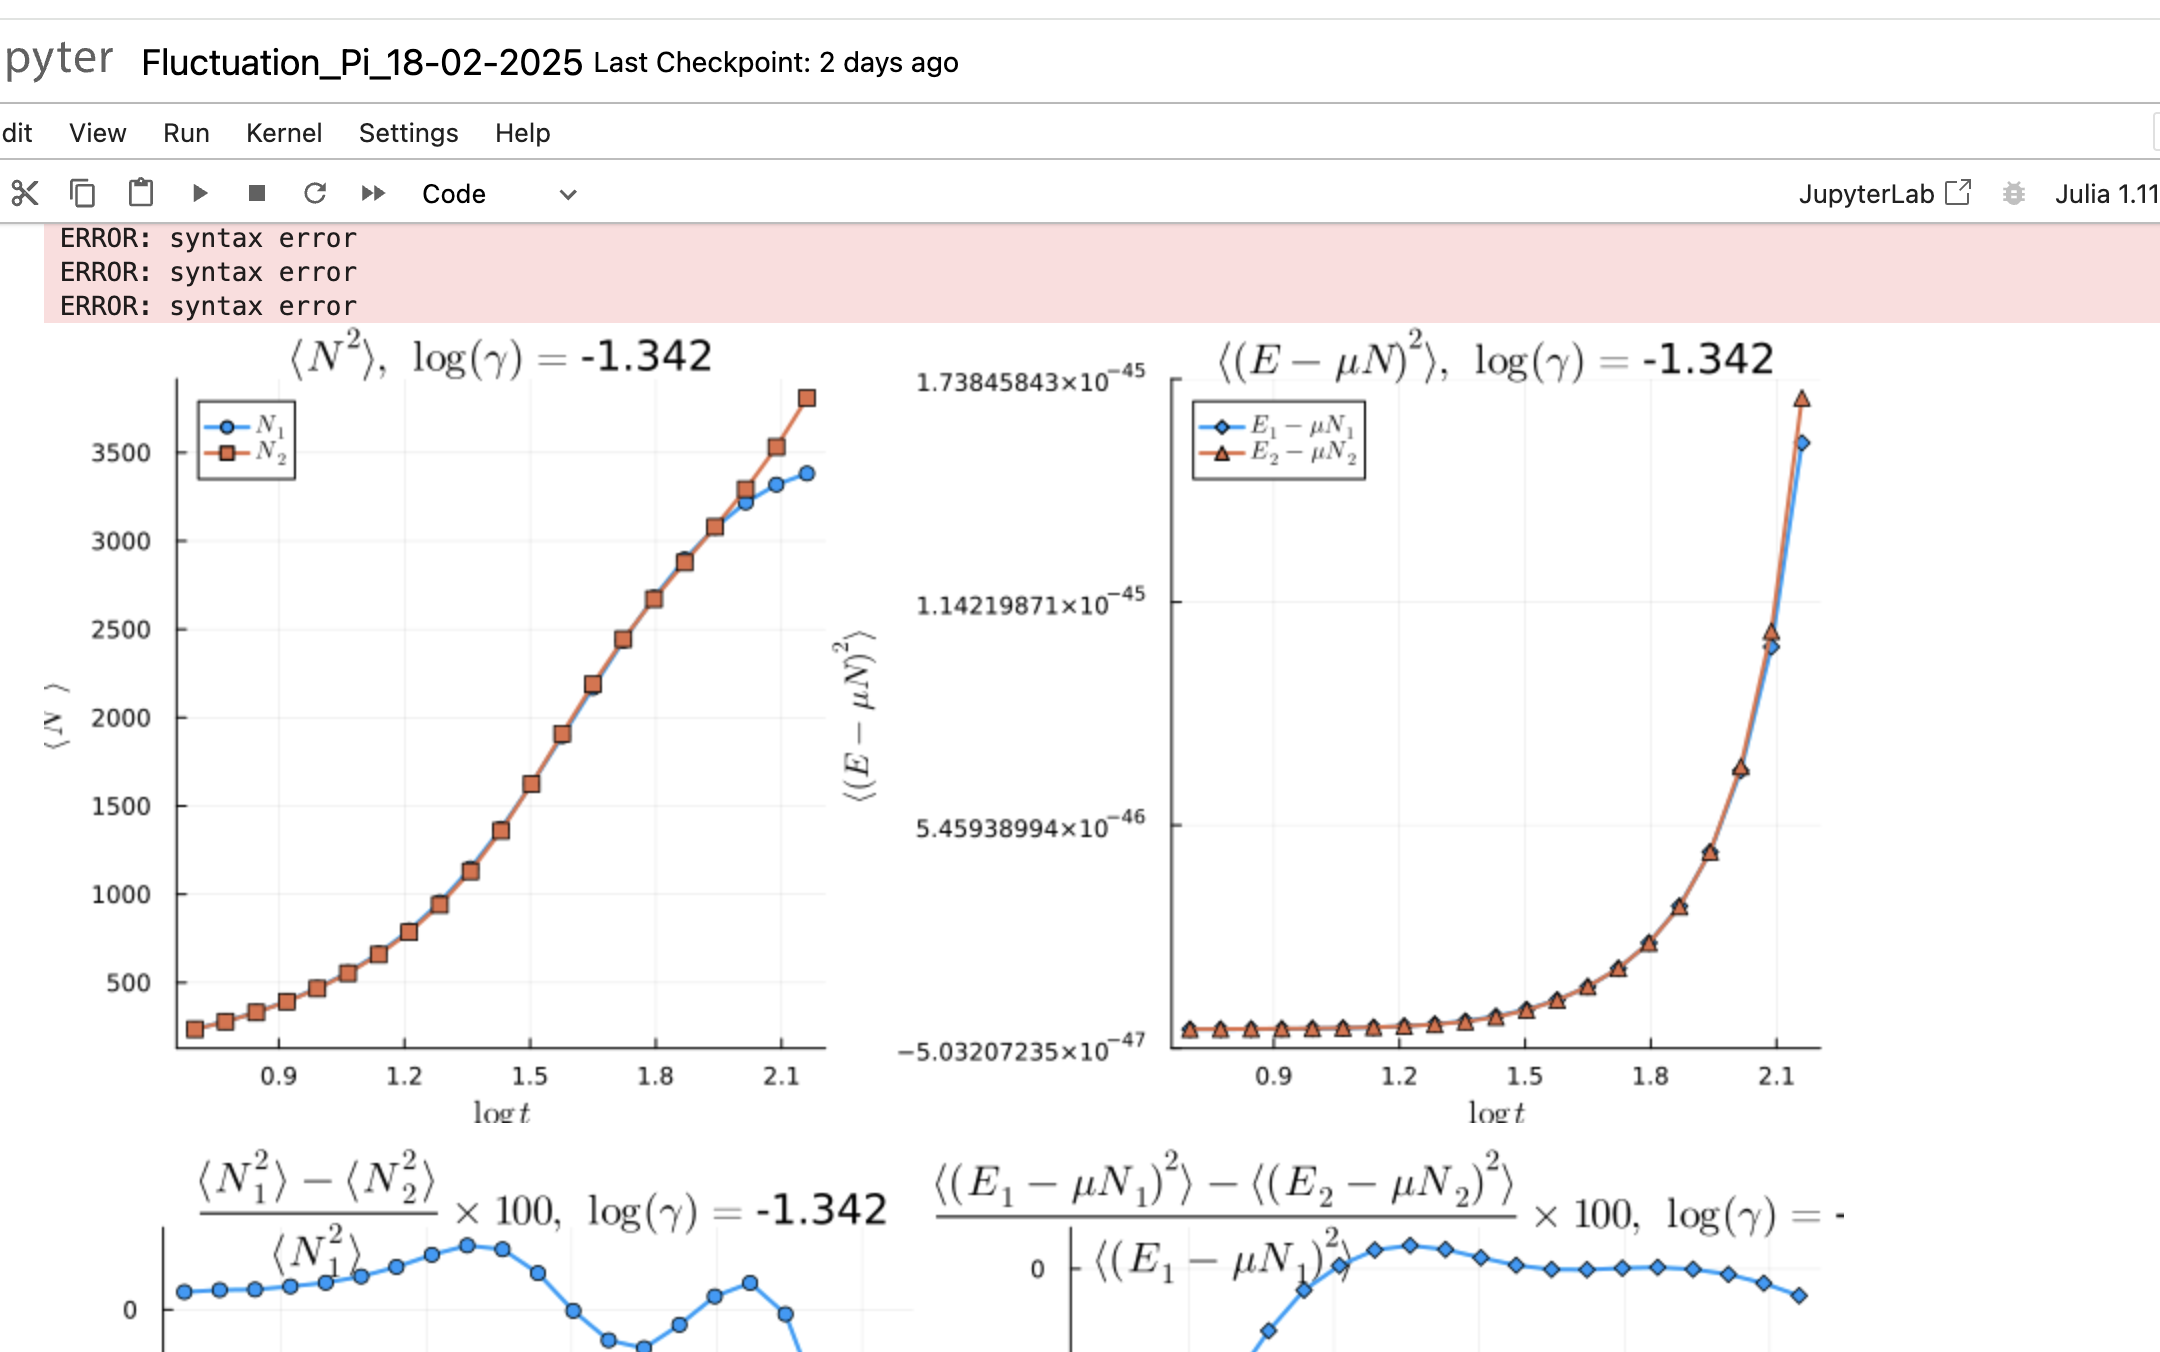
\includegraphics[width=1\textwidth]{Figures/test}

%\begin{aff}
%Donc une a l'ordre un en $\delta \theta (\operator{A}^{(0)})^{-1} %\operator{V}$ 

%\begin{eqnarray*}
%	\langle \delta \Pi ( \theta) \delta \Pi ( \theta') \rangle & = &  ( (\Pi^c_s - \Pi^c)\Pi^c/\Pi^c_s ) ( \theta ) \delta_{\theta, \theta'}/\delta \theta + \mathscr{F}(\theta , \theta' ) ,	
%\end{eqnarray*}

%avec 

%\begin{eqnarray*}
%	\mathscr{F}(\theta , \theta' ) & = & \left [ (\Pi^c_s - \Pi^c )( \theta)  +  (\Pi^c_s - \Pi^c ) ( \theta' )\right ] \frac{\Pi^c}{\Pi^c_s}(\theta)\frac{\Pi^c}{\Pi^c_s}(\theta') \frac{ \Delta( \theta'- \theta )}{ 2 \pi }\\
%	&&  - \left [ (\Pi^c_s - \Pi^c )( \theta)   (\Pi^c_s - \Pi^c ) ( \theta' )\right ] \frac{\Pi^c}{\Pi^c_s}(\theta)\frac{\Pi^c}{\Pi^c_s}(\theta')\int d\theta'' \left (   \frac{ \Pi^c/\Pi^c_s}{\Pi^c_s - \Pi^c} \right )(\theta'') \frac{\Delta(\theta''- \theta)}{2 \pi}\frac{\Delta(\theta''- \theta')}{2 \pi}  	
%\end{eqnarray*}
%\end{aff}



 









\subsection{États du vide et pseudovacuum}
%Dans ce chapitre, nous nous intéressons aux fluctuations de la distribution de rapidité \( \delta \rho \) autour d'une distribution de référence \( \rho^c \), qui maximise la contribution à la fonction de partition des états, exprimée comme une fonctionnelle de la distribution \( \rho \) : 

La fonction de partition des états, s'exprime comme une fonctionnelle de la distribution \( \rho \) : 

\begin{eqnarray*}
	\Xi & = & \sum_\rho \exp \left( -\mathcal{A}(\rho) \right).
\end{eqnarray*}  

Dans la section {\em \bf Entropie de Yang-Yang} (\ref{??}), l'action \( \mathcal{A}(\rho) \) s'écrit sous la forme :  

\begin{eqnarray*}
	\mathcal{A}(\rho) & \doteq & - L\mathcal{S}_{YY}(\rho) + L\int f(\theta) \rho (\theta) \, d\theta,		
\end{eqnarray*}  

où \( \mathcal{S}_{YY} \) est la fonctionnelle d'entropie de Yang-Yang, définie dans (\ref{??}), et \( f \) est la fonction paramétrant les charges, introduite dans (\ref{??}).  

Dans cette même section {\em \bf Entropie de Yang-Yang} (\ref{??}), nous avons établi un lien entre \( f \) et distribution de référence \( \rho^c \), qui maximise la contribution à la fonction de partition des états .\\

On veux tester si nos experience est décrit pas un GGE. Pour cela nous nous intéressons aux fluctuations de la distribution de rapidité \( \delta \rho \) autour \( \rho^c \).

%Nous poursuivons à présent avec cette définition de l'action de classe $\mathcal{C}^2$ et admetant une distribution critique $\rho^c$ tel que sa différentielle en ce point critique soit nulle $d\mathcal{A}_{\rho^c} = 0 $ (\ref{??}) de sorte que d'aprés la formule de Taylor-Youg %afin de déterminer les fluctuations autour de \( \Pi^c \). Pour cela, nous réécrivons l'action sous la forme :  

Nous poursuivons à présent avec cette définition de l'action de classe $\mathcal{C}^2$ et admetant une distribution critique $\rho^c$ tel que sa différentielle en ce point critique soit nulle $d\mathcal{A}_{\rho^c} = 0 $ (\ref{??}) de sorte que d'aprés la formule de Taylor-Youg %afin de déterminer les fluctuations autour de \( \Pi^c \). Pour cela, nous réécrivons l'action sous la forme :  

\begin{eqnarray*}  
	\mathcal{A}(\rho^c + \delta \rho) & \underset{ \delta \rho \to 0 }{=} & \mathcal{A}(\rho^c)  + \frac{1}{2} \left. \frac{\delta^2 \mathcal{A}}{\delta \rho^2} \right|_{\rho^c} (\delta \rho) + \mathcal{O}((\delta \rho)^3),  
\end{eqnarray*}  

une expression quadratique pour l'action à l'ordre dominant en \( \delta \Pi \) avec $\left. \frac{\delta^2 \mathcal{A}}{\delta \rho^2} \right|_{\rho^c}$ la forme quadratique définie positive (Fig (\ref{fig.fluctu.A})).

\begin{figure}[H]
	\centering 
	\begin{tikzpicture}
		\begin{scope}[shift={(0,0)}]
			\begin{scope}[transform canvas={scale=0.6}]
				\input{Figures/Fonc_A_code}	
			
			\end{scope}
			
			\draw[color = red , scale = 0.5 , draw = none  ] (-2 , -1) rectangle (5, 6) ; 	
		\end{scope}
		
		\begin{scope}[shift={(19,-1)}]
			\begin{scope}[transform canvas={scale=0.6}]
				\input{Figures/Occupation_theta_code}	
			
			\end{scope}
			\begin{scope}[scale=1]
				\draw[color = red , scale = 1 , draw = none  ] (-1 , -1) rectangle (5, 5) ; 
			\end{scope}	
		\end{scope}

		
				
			
	\end{tikzpicture}	
	\captionsetup{skip=10pt} % Ajoute de l’espace après la légende
	\label{fig.fluctu.A}
\end{figure}


On discrétise l'axe des rapidités en  petite cellule de rapidité $[\theta, \theta+\delta\theta]$, qui contient $L\rho(\theta) \delta \theta$ rapidités. 
	



Avec ces petites tranches, la forme quadratique s’écrit :

\begin{eqnarray*}
    \left. \frac{\delta^2 \mathcal{A}}{{\delta \rho}^2} \right|_{\rho^c}(\delta \rho ) &=&  \sum_{a,b \mid \text{tranche}}  
    \delta \rho(\theta_a)  \frac{\partial^2 \mathcal{A}}{\partial \delta \rho(\theta_a) \partial \delta \rho(\theta_b) } (\rho^c)  \delta \rho(\theta_b).
\end{eqnarray*}
Les fluctuations s’écrivent donc :

\begin{eqnarray*}
    \langle \delta \rho ( \theta) \delta \rho ( \theta') \rangle &=&  
    \frac{ \int d\delta \rho \, \delta \rho(\theta) \delta \rho ( \theta') 
    \exp \left( - \frac{1}{2} \sum_{a,b \mid \text{tranche}}  
    \delta \rho(\theta_a) \frac{\partial^2 \mathcal{A}}{\partial \delta \rho(\theta_a) \partial \delta \rho(\theta_b) } (\rho^c)  \delta \rho(\theta_b) \right) }
    { \int d\delta \Pi  
    \exp \left( - \frac{1}{2} \sum_{a,b \mid \text{tranche}}  
    \delta \rho(\theta_a) \frac{\partial^2 \mathcal{A}}{\partial \delta \rho(\theta_a) \partial \delta \rho(\theta_b) } (\rho^c)  \delta \rho(\theta_b) \right) } \\
    &=& \left( \mathbf{A}^{-1} \right)_{\theta , \theta'}
\end{eqnarray*}


\begin{aff}

\begin{eqnarray*}
	\langle \delta \rho ( \theta) \delta \rho ( \theta') \rangle &=& 	\left( \mathbf{A}^{-1} \right)_{\theta , \theta'}
\end{eqnarray*}

	
avec la  {\em matrice hessienne} $\mathbf{A}_{\theta , \theta'} \equiv \frac{\partial^2 \mathcal{A}}{\partial \delta \rho(\theta) \partial \delta \rho(\theta') }(\rho^c)$, au point critique/ qui maximise la probabilité  $\rho^c=\rho^c_s \nu^c $, s'écrit

\begin{eqnarray*}
	\operator{A} & = & \operator{A}^{(0)} + \delta \theta \operator{V}
\end{eqnarray*}

avec 

\begin{eqnarray*}
	A^{(0)}_{\theta , \theta'}  & = &  L\delta \theta \left ( \frac{ 1}{\rho^c_s ( 1  - \nu^c ) \nu^c } \right )(\theta)    \delta({\theta - \theta '})	,\\
	V_{\theta , \theta'}  &= & L \delta \theta \left \{ - \left [ \left ( \frac{1}{\rho^c_s( 1 - \nu^c) } \right ) ( \theta)  +  \left ( \frac{1}{\rho^c_s( 1 - \nu^c) } \right ) ( \theta' )\right ] \frac{ \Delta( \theta'- \theta )}{ 2 \pi } + \int d\theta''  \left ( \frac{\nu^c}{\rho^c_s( 1 - \nu^c) } \right )(\theta'') \frac{\Delta(\theta''- \theta)}{2 \pi}\frac{\Delta(\theta''- \theta')}{2 \pi}   \right \} 	
\end{eqnarray*}

\end{aff}

\subsection{Testes}

\begin{eqnarray*}
	\Delta_{\operator{\mathcal{N}}}^2  & = &  \frac{1}{\beta} \left . \frac{\partial \langle \operator{\mathcal{N}} \rangle}{\partial \mu} \right )_T \\
	\Delta_{\operator{\mathcal{E}}-\mu \operator{\mathcal{N}}}^2  & = &  - \left . \frac{\partial \langle \operator{\mathcal{E}}-\mu \operator{\mathcal{N}} \rangle}{\partial \beta} \right )_\mu 
\end{eqnarray*}

et 

\begin{eqnarray*}
	\Delta_{\operator{\mathcal{N}}}^2  &= & L^2 \int d\theta_a \int d \theta_b \, \langle \delta \rho(\theta_a) \delta \rho(\theta_b) \rangle \\
	\Delta_{\operator{\mathcal{E}}-\mu \operator{\mathcal{N}}}^2  & = & L^2 \int d\theta_a \int d \theta_b \, \left ( - \mu + \frac{1}2 m \theta_a^2  \right  )\left ( - \mu + \frac{1}2 m \theta_b^2  \right  )  \langle \delta \rho(\theta_a) \delta \rho(\theta_b) \rangle
\end{eqnarray*}

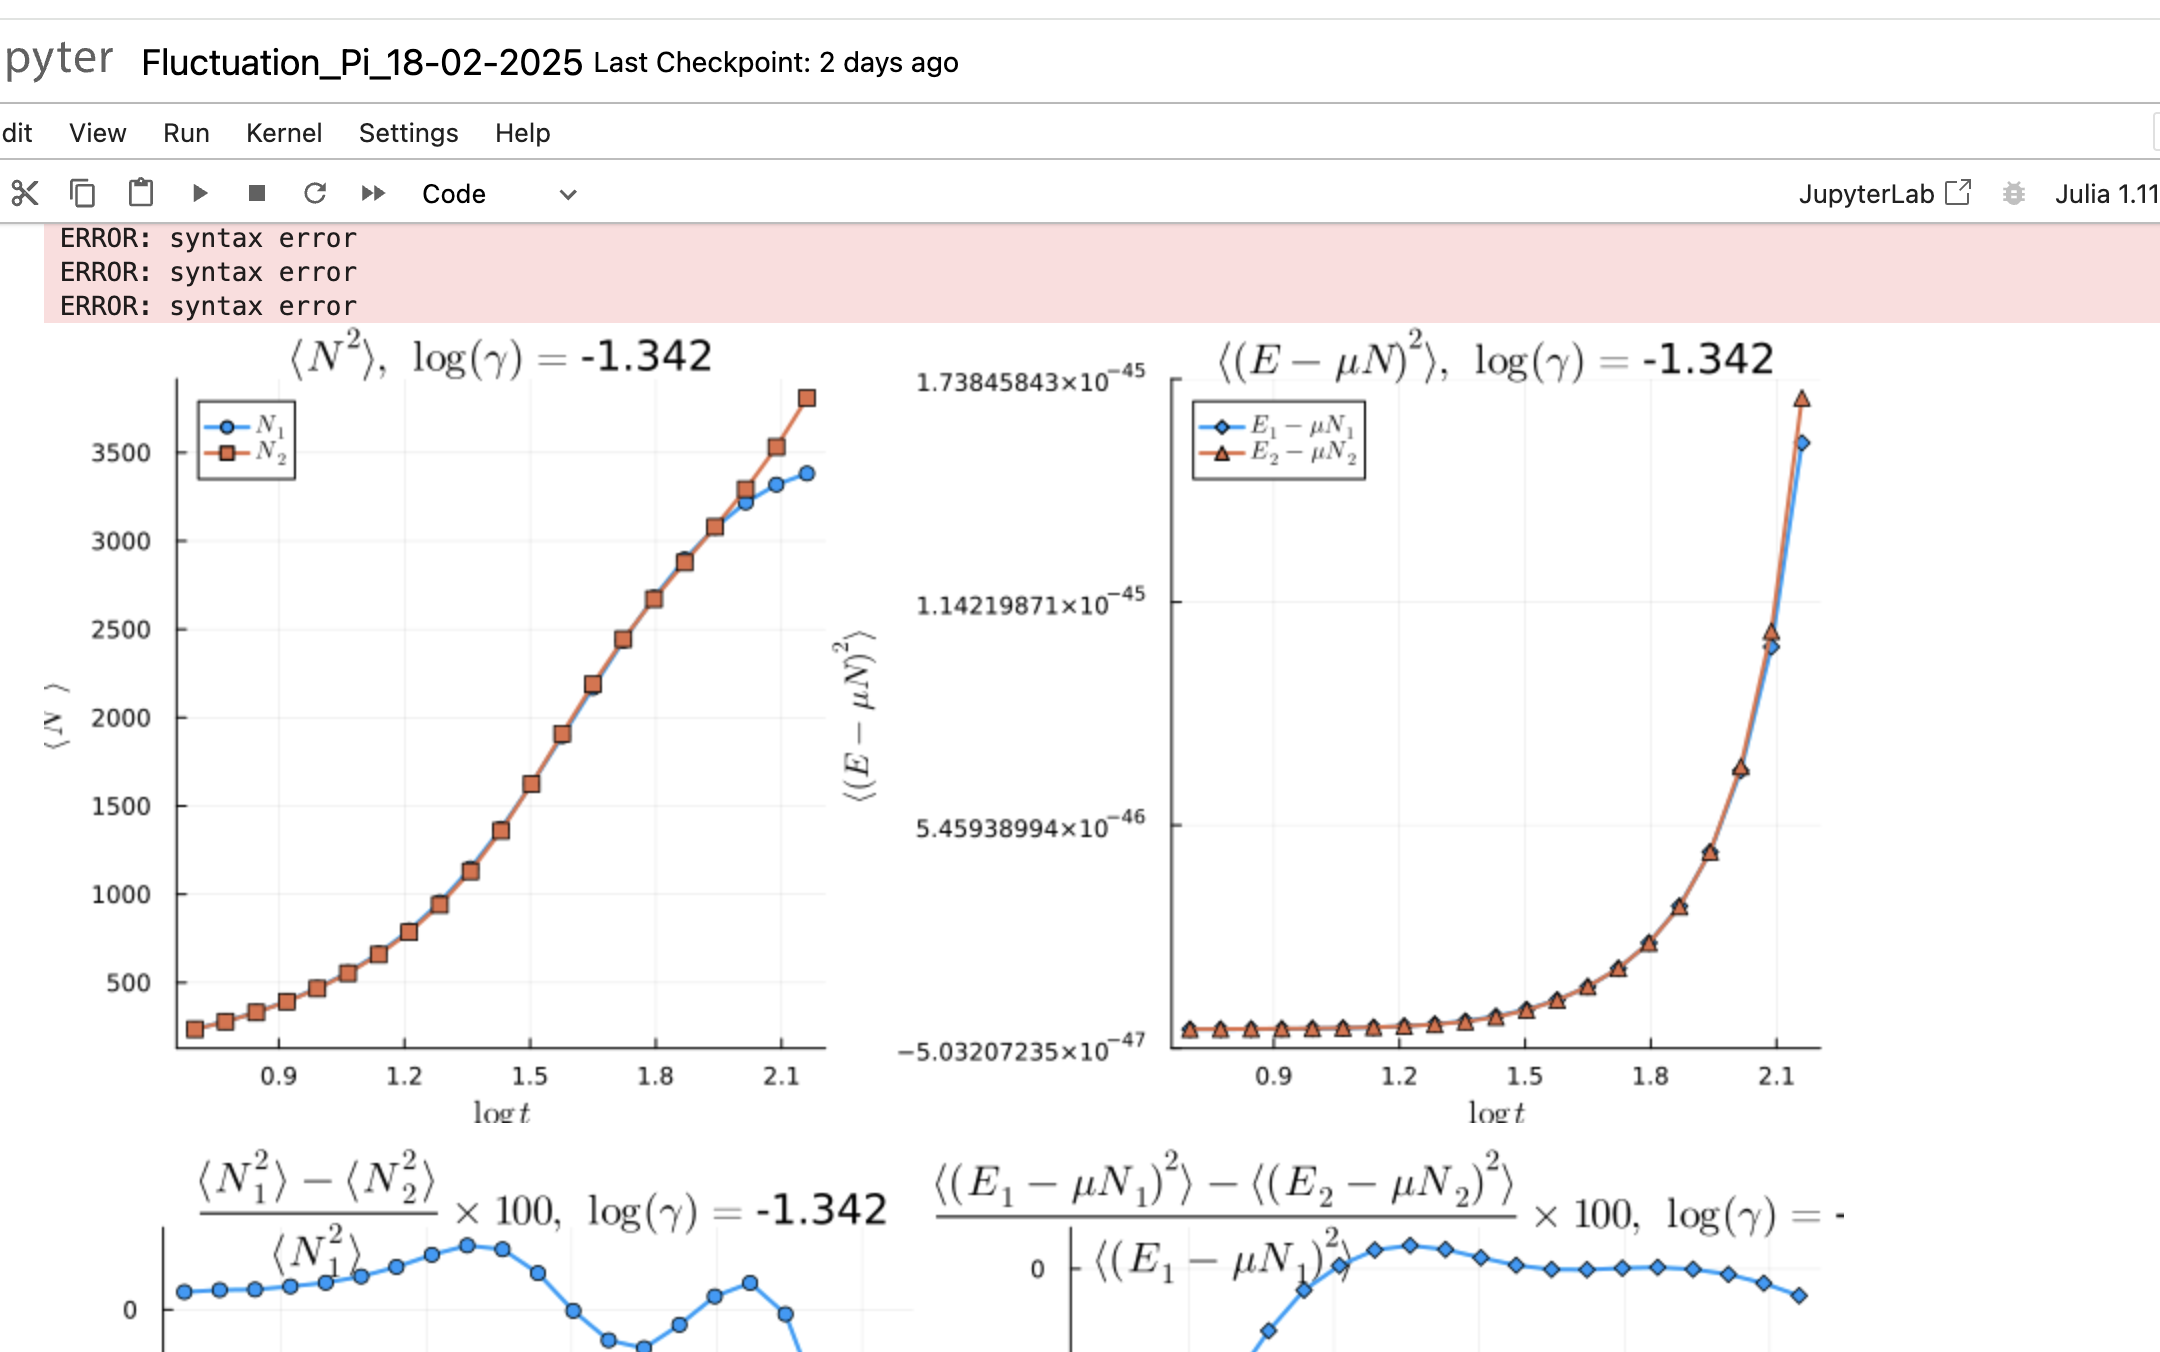
\includegraphics[width=1\textwidth]{Figures/test}

%\begin{aff}
%Donc une a l'ordre un en $\delta \theta (\operator{A}^{(0)})^{-1} %\operator{V}$ 

%\begin{eqnarray*}
%	\langle \delta \Pi ( \theta) \delta \Pi ( \theta') \rangle & = &  ( (\Pi^c_s - \Pi^c)\Pi^c/\Pi^c_s ) ( \theta ) \delta_{\theta, \theta'}/\delta \theta + \mathscr{F}(\theta , \theta' ) ,	
%\end{eqnarray*}

%avec 

%\begin{eqnarray*}
%	\mathscr{F}(\theta , \theta' ) & = & \left [ (\Pi^c_s - \Pi^c )( \theta)  +  (\Pi^c_s - \Pi^c ) ( \theta' )\right ] \frac{\Pi^c}{\Pi^c_s}(\theta)\frac{\Pi^c}{\Pi^c_s}(\theta') \frac{ \Delta( \theta'- \theta )}{ 2 \pi }\\
%	&&  - \left [ (\Pi^c_s - \Pi^c )( \theta)   (\Pi^c_s - \Pi^c ) ( \theta' )\right ] \frac{\Pi^c}{\Pi^c_s}(\theta)\frac{\Pi^c}{\Pi^c_s}(\theta')\int d\theta'' \left (   \frac{ \Pi^c/\Pi^c_s}{\Pi^c_s - \Pi^c} \right )(\theta'') \frac{\Delta(\theta''- \theta)}{2 \pi}\frac{\Delta(\theta''- \theta')}{2 \pi}  	
%\end{eqnarray*}
%\end{aff}



 










\subsection{Opérateurs conservés (intégrales du mouvement)}
%Dans ce chapitre, nous nous intéressons aux fluctuations de la distribution de rapidité \( \delta \rho \) autour d'une distribution de référence \( \rho^c \), qui maximise la contribution à la fonction de partition des états, exprimée comme une fonctionnelle de la distribution \( \rho \) : 

La fonction de partition des états, s'exprime comme une fonctionnelle de la distribution \( \rho \) : 

\begin{eqnarray*}
	\Xi & = & \sum_\rho \exp \left( -\mathcal{A}(\rho) \right).
\end{eqnarray*}  

Dans la section {\em \bf Entropie de Yang-Yang} (\ref{??}), l'action \( \mathcal{A}(\rho) \) s'écrit sous la forme :  

\begin{eqnarray*}
	\mathcal{A}(\rho) & \doteq & - L\mathcal{S}_{YY}(\rho) + L\int f(\theta) \rho (\theta) \, d\theta,		
\end{eqnarray*}  

où \( \mathcal{S}_{YY} \) est la fonctionnelle d'entropie de Yang-Yang, définie dans (\ref{??}), et \( f \) est la fonction paramétrant les charges, introduite dans (\ref{??}).  

Dans cette même section {\em \bf Entropie de Yang-Yang} (\ref{??}), nous avons établi un lien entre \( f \) et distribution de référence \( \rho^c \), qui maximise la contribution à la fonction de partition des états .\\

On veux tester si nos experience est décrit pas un GGE. Pour cela nous nous intéressons aux fluctuations de la distribution de rapidité \( \delta \rho \) autour \( \rho^c \).

%Nous poursuivons à présent avec cette définition de l'action de classe $\mathcal{C}^2$ et admetant une distribution critique $\rho^c$ tel que sa différentielle en ce point critique soit nulle $d\mathcal{A}_{\rho^c} = 0 $ (\ref{??}) de sorte que d'aprés la formule de Taylor-Youg %afin de déterminer les fluctuations autour de \( \Pi^c \). Pour cela, nous réécrivons l'action sous la forme :  

Nous poursuivons à présent avec cette définition de l'action de classe $\mathcal{C}^2$ et admetant une distribution critique $\rho^c$ tel que sa différentielle en ce point critique soit nulle $d\mathcal{A}_{\rho^c} = 0 $ (\ref{??}) de sorte que d'aprés la formule de Taylor-Youg %afin de déterminer les fluctuations autour de \( \Pi^c \). Pour cela, nous réécrivons l'action sous la forme :  

\begin{eqnarray*}  
	\mathcal{A}(\rho^c + \delta \rho) & \underset{ \delta \rho \to 0 }{=} & \mathcal{A}(\rho^c)  + \frac{1}{2} \left. \frac{\delta^2 \mathcal{A}}{\delta \rho^2} \right|_{\rho^c} (\delta \rho) + \mathcal{O}((\delta \rho)^3),  
\end{eqnarray*}  

une expression quadratique pour l'action à l'ordre dominant en \( \delta \Pi \) avec $\left. \frac{\delta^2 \mathcal{A}}{\delta \rho^2} \right|_{\rho^c}$ la forme quadratique définie positive (Fig (\ref{fig.fluctu.A})).

\begin{figure}[H]
	\centering 
	\begin{tikzpicture}
		\begin{scope}[shift={(0,0)}]
			\begin{scope}[transform canvas={scale=0.6}]
				\input{Figures/Fonc_A_code}	
			
			\end{scope}
			
			\draw[color = red , scale = 0.5 , draw = none  ] (-2 , -1) rectangle (5, 6) ; 	
		\end{scope}
		
		\begin{scope}[shift={(19,-1)}]
			\begin{scope}[transform canvas={scale=0.6}]
				\input{Figures/Occupation_theta_code}	
			
			\end{scope}
			\begin{scope}[scale=1]
				\draw[color = red , scale = 1 , draw = none  ] (-1 , -1) rectangle (5, 5) ; 
			\end{scope}	
		\end{scope}

		
				
			
	\end{tikzpicture}	
	\captionsetup{skip=10pt} % Ajoute de l’espace après la légende
	\label{fig.fluctu.A}
\end{figure}


On discrétise l'axe des rapidités en  petite cellule de rapidité $[\theta, \theta+\delta\theta]$, qui contient $L\rho(\theta) \delta \theta$ rapidités. 
	



Avec ces petites tranches, la forme quadratique s’écrit :

\begin{eqnarray*}
    \left. \frac{\delta^2 \mathcal{A}}{{\delta \rho}^2} \right|_{\rho^c}(\delta \rho ) &=&  \sum_{a,b \mid \text{tranche}}  
    \delta \rho(\theta_a)  \frac{\partial^2 \mathcal{A}}{\partial \delta \rho(\theta_a) \partial \delta \rho(\theta_b) } (\rho^c)  \delta \rho(\theta_b).
\end{eqnarray*}
Les fluctuations s’écrivent donc :

\begin{eqnarray*}
    \langle \delta \rho ( \theta) \delta \rho ( \theta') \rangle &=&  
    \frac{ \int d\delta \rho \, \delta \rho(\theta) \delta \rho ( \theta') 
    \exp \left( - \frac{1}{2} \sum_{a,b \mid \text{tranche}}  
    \delta \rho(\theta_a) \frac{\partial^2 \mathcal{A}}{\partial \delta \rho(\theta_a) \partial \delta \rho(\theta_b) } (\rho^c)  \delta \rho(\theta_b) \right) }
    { \int d\delta \Pi  
    \exp \left( - \frac{1}{2} \sum_{a,b \mid \text{tranche}}  
    \delta \rho(\theta_a) \frac{\partial^2 \mathcal{A}}{\partial \delta \rho(\theta_a) \partial \delta \rho(\theta_b) } (\rho^c)  \delta \rho(\theta_b) \right) } \\
    &=& \left( \mathbf{A}^{-1} \right)_{\theta , \theta'}
\end{eqnarray*}


\begin{aff}

\begin{eqnarray*}
	\langle \delta \rho ( \theta) \delta \rho ( \theta') \rangle &=& 	\left( \mathbf{A}^{-1} \right)_{\theta , \theta'}
\end{eqnarray*}

	
avec la  {\em matrice hessienne} $\mathbf{A}_{\theta , \theta'} \equiv \frac{\partial^2 \mathcal{A}}{\partial \delta \rho(\theta) \partial \delta \rho(\theta') }(\rho^c)$, au point critique/ qui maximise la probabilité  $\rho^c=\rho^c_s \nu^c $, s'écrit

\begin{eqnarray*}
	\operator{A} & = & \operator{A}^{(0)} + \delta \theta \operator{V}
\end{eqnarray*}

avec 

\begin{eqnarray*}
	A^{(0)}_{\theta , \theta'}  & = &  L\delta \theta \left ( \frac{ 1}{\rho^c_s ( 1  - \nu^c ) \nu^c } \right )(\theta)    \delta({\theta - \theta '})	,\\
	V_{\theta , \theta'}  &= & L \delta \theta \left \{ - \left [ \left ( \frac{1}{\rho^c_s( 1 - \nu^c) } \right ) ( \theta)  +  \left ( \frac{1}{\rho^c_s( 1 - \nu^c) } \right ) ( \theta' )\right ] \frac{ \Delta( \theta'- \theta )}{ 2 \pi } + \int d\theta''  \left ( \frac{\nu^c}{\rho^c_s( 1 - \nu^c) } \right )(\theta'') \frac{\Delta(\theta''- \theta)}{2 \pi}\frac{\Delta(\theta''- \theta')}{2 \pi}   \right \} 	
\end{eqnarray*}

\end{aff}

\subsection{Testes}

\begin{eqnarray*}
	\Delta_{\operator{\mathcal{N}}}^2  & = &  \frac{1}{\beta} \left . \frac{\partial \langle \operator{\mathcal{N}} \rangle}{\partial \mu} \right )_T \\
	\Delta_{\operator{\mathcal{E}}-\mu \operator{\mathcal{N}}}^2  & = &  - \left . \frac{\partial \langle \operator{\mathcal{E}}-\mu \operator{\mathcal{N}} \rangle}{\partial \beta} \right )_\mu 
\end{eqnarray*}

et 

\begin{eqnarray*}
	\Delta_{\operator{\mathcal{N}}}^2  &= & L^2 \int d\theta_a \int d \theta_b \, \langle \delta \rho(\theta_a) \delta \rho(\theta_b) \rangle \\
	\Delta_{\operator{\mathcal{E}}-\mu \operator{\mathcal{N}}}^2  & = & L^2 \int d\theta_a \int d \theta_b \, \left ( - \mu + \frac{1}2 m \theta_a^2  \right  )\left ( - \mu + \frac{1}2 m \theta_b^2  \right  )  \langle \delta \rho(\theta_a) \delta \rho(\theta_b) \rangle
\end{eqnarray*}

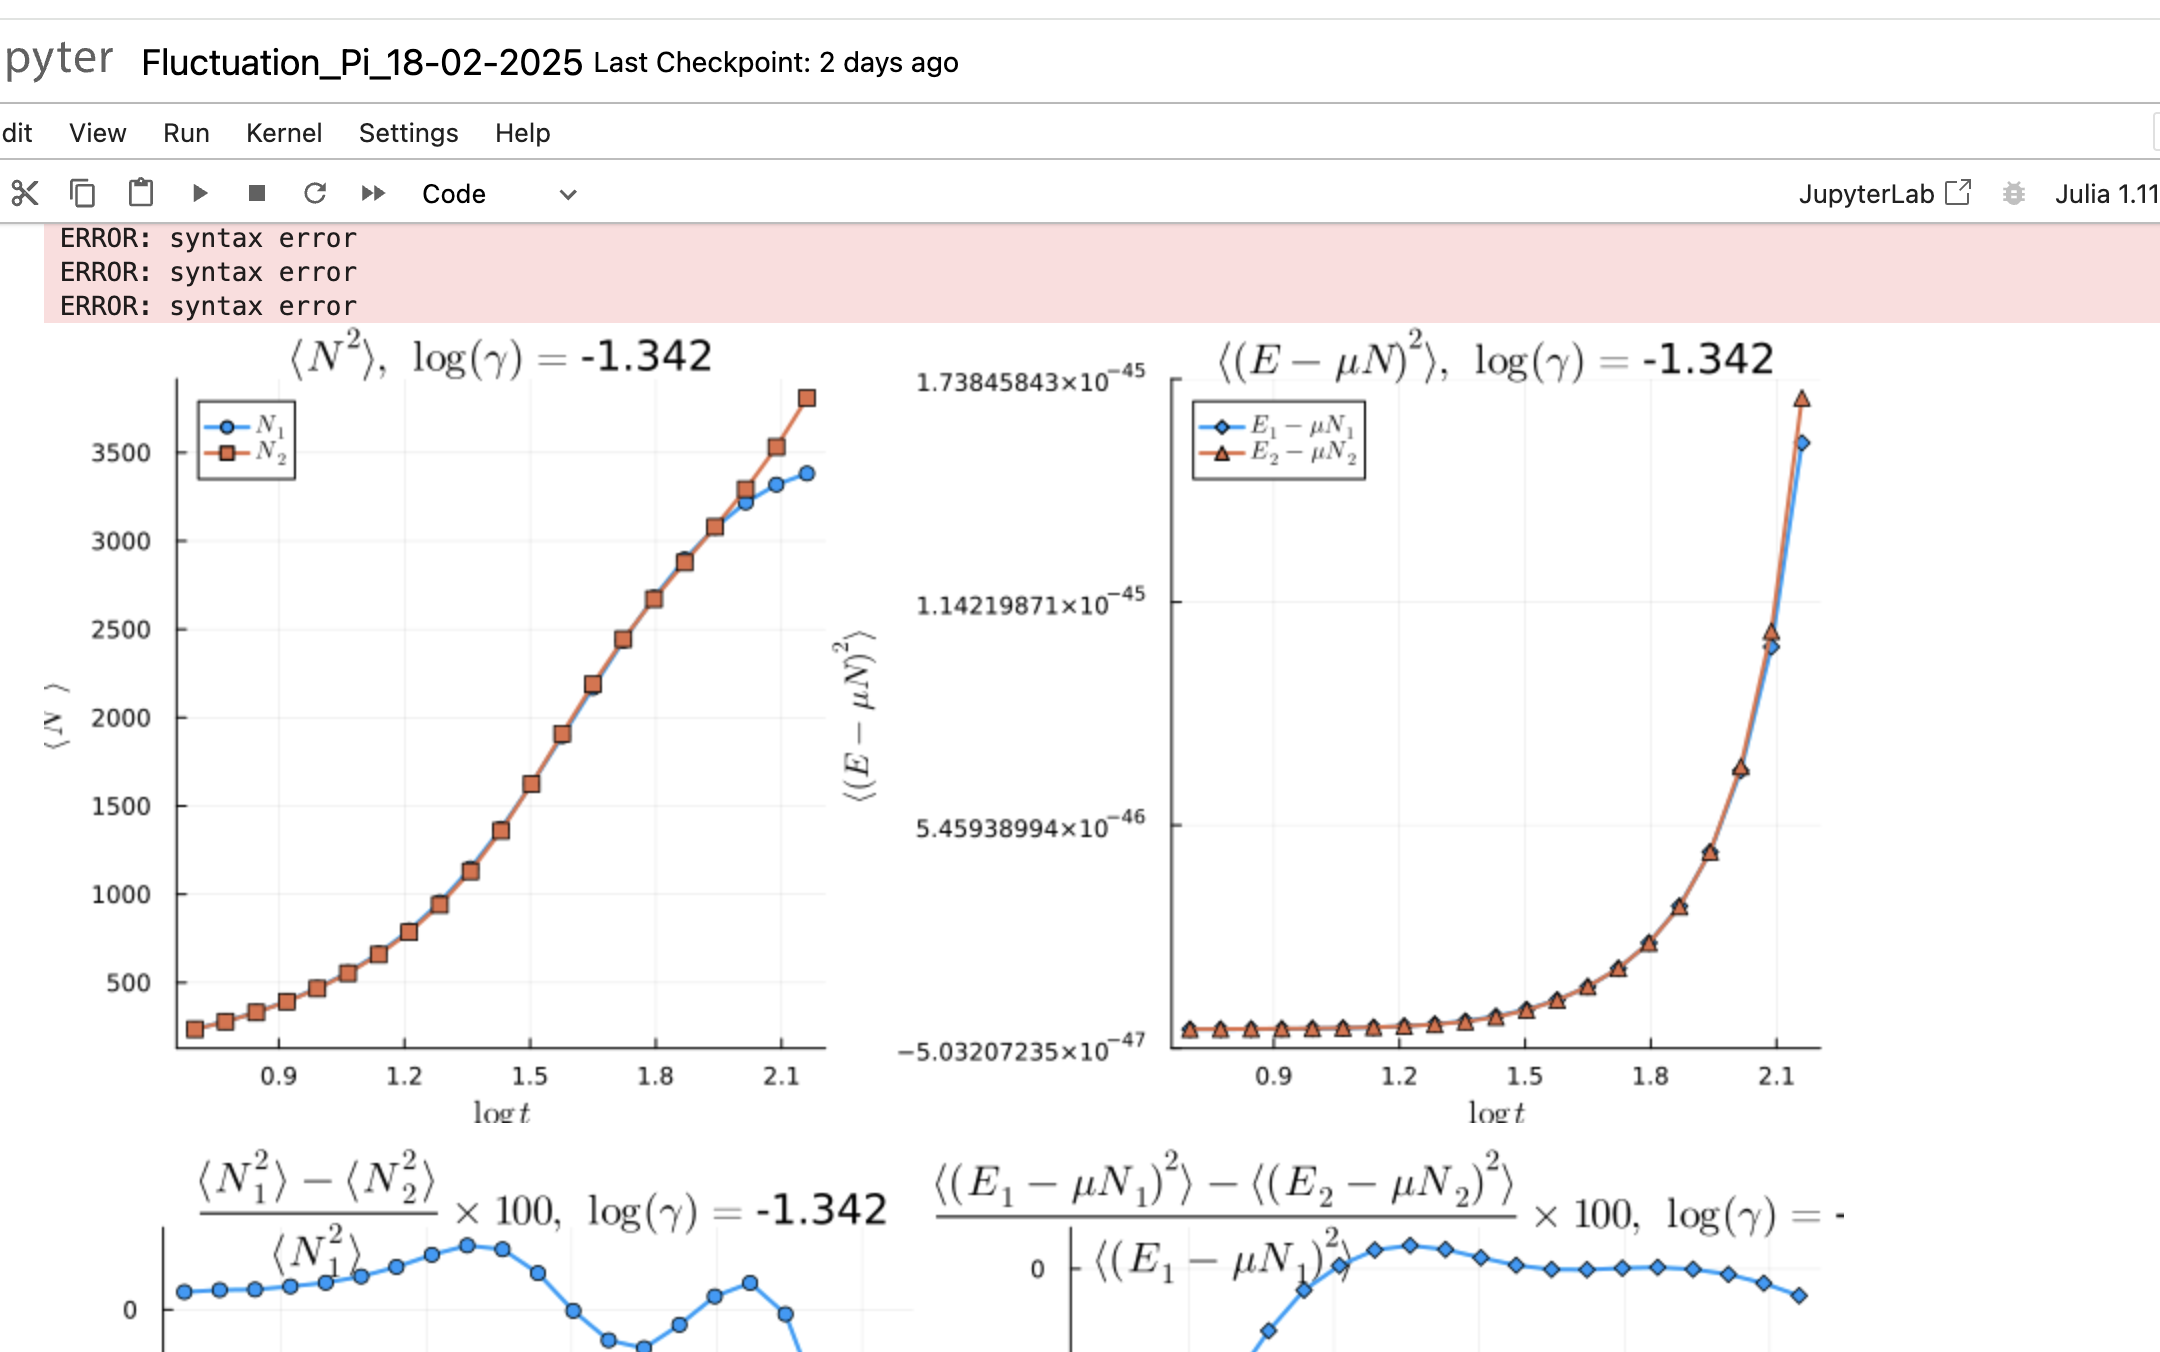
\includegraphics[width=1\textwidth]{Figures/test}

%\begin{aff}
%Donc une a l'ordre un en $\delta \theta (\operator{A}^{(0)})^{-1} %\operator{V}$ 

%\begin{eqnarray*}
%	\langle \delta \Pi ( \theta) \delta \Pi ( \theta') \rangle & = &  ( (\Pi^c_s - \Pi^c)\Pi^c/\Pi^c_s ) ( \theta ) \delta_{\theta, \theta'}/\delta \theta + \mathscr{F}(\theta , \theta' ) ,	
%\end{eqnarray*}

%avec 

%\begin{eqnarray*}
%	\mathscr{F}(\theta , \theta' ) & = & \left [ (\Pi^c_s - \Pi^c )( \theta)  +  (\Pi^c_s - \Pi^c ) ( \theta' )\right ] \frac{\Pi^c}{\Pi^c_s}(\theta)\frac{\Pi^c}{\Pi^c_s}(\theta') \frac{ \Delta( \theta'- \theta )}{ 2 \pi }\\
%	&&  - \left [ (\Pi^c_s - \Pi^c )( \theta)   (\Pi^c_s - \Pi^c ) ( \theta' )\right ] \frac{\Pi^c}{\Pi^c_s}(\theta)\frac{\Pi^c}{\Pi^c_s}(\theta')\int d\theta'' \left (   \frac{ \Pi^c/\Pi^c_s}{\Pi^c_s - \Pi^c} \right )(\theta'') \frac{\Delta(\theta''- \theta)}{2 \pi}\frac{\Delta(\theta''- \theta')}{2 \pi}  	
%\end{eqnarray*}
%\end{aff}



 








 
\subsection{Fonction d’onde $\chi_N$ et Hamiltonien et moment à N corps}
%Dans ce chapitre, nous nous intéressons aux fluctuations de la distribution de rapidité \( \delta \rho \) autour d'une distribution de référence \( \rho^c \), qui maximise la contribution à la fonction de partition des états, exprimée comme une fonctionnelle de la distribution \( \rho \) : 

La fonction de partition des états, s'exprime comme une fonctionnelle de la distribution \( \rho \) : 

\begin{eqnarray*}
	\Xi & = & \sum_\rho \exp \left( -\mathcal{A}(\rho) \right).
\end{eqnarray*}  

Dans la section {\em \bf Entropie de Yang-Yang} (\ref{??}), l'action \( \mathcal{A}(\rho) \) s'écrit sous la forme :  

\begin{eqnarray*}
	\mathcal{A}(\rho) & \doteq & - L\mathcal{S}_{YY}(\rho) + L\int f(\theta) \rho (\theta) \, d\theta,		
\end{eqnarray*}  

où \( \mathcal{S}_{YY} \) est la fonctionnelle d'entropie de Yang-Yang, définie dans (\ref{??}), et \( f \) est la fonction paramétrant les charges, introduite dans (\ref{??}).  

Dans cette même section {\em \bf Entropie de Yang-Yang} (\ref{??}), nous avons établi un lien entre \( f \) et distribution de référence \( \rho^c \), qui maximise la contribution à la fonction de partition des états .\\

On veux tester si nos experience est décrit pas un GGE. Pour cela nous nous intéressons aux fluctuations de la distribution de rapidité \( \delta \rho \) autour \( \rho^c \).

%Nous poursuivons à présent avec cette définition de l'action de classe $\mathcal{C}^2$ et admetant une distribution critique $\rho^c$ tel que sa différentielle en ce point critique soit nulle $d\mathcal{A}_{\rho^c} = 0 $ (\ref{??}) de sorte que d'aprés la formule de Taylor-Youg %afin de déterminer les fluctuations autour de \( \Pi^c \). Pour cela, nous réécrivons l'action sous la forme :  

Nous poursuivons à présent avec cette définition de l'action de classe $\mathcal{C}^2$ et admetant une distribution critique $\rho^c$ tel que sa différentielle en ce point critique soit nulle $d\mathcal{A}_{\rho^c} = 0 $ (\ref{??}) de sorte que d'aprés la formule de Taylor-Youg %afin de déterminer les fluctuations autour de \( \Pi^c \). Pour cela, nous réécrivons l'action sous la forme :  

\begin{eqnarray*}  
	\mathcal{A}(\rho^c + \delta \rho) & \underset{ \delta \rho \to 0 }{=} & \mathcal{A}(\rho^c)  + \frac{1}{2} \left. \frac{\delta^2 \mathcal{A}}{\delta \rho^2} \right|_{\rho^c} (\delta \rho) + \mathcal{O}((\delta \rho)^3),  
\end{eqnarray*}  

une expression quadratique pour l'action à l'ordre dominant en \( \delta \Pi \) avec $\left. \frac{\delta^2 \mathcal{A}}{\delta \rho^2} \right|_{\rho^c}$ la forme quadratique définie positive (Fig (\ref{fig.fluctu.A})).

\begin{figure}[H]
	\centering 
	\begin{tikzpicture}
		\begin{scope}[shift={(0,0)}]
			\begin{scope}[transform canvas={scale=0.6}]
				\input{Figures/Fonc_A_code}	
			
			\end{scope}
			
			\draw[color = red , scale = 0.5 , draw = none  ] (-2 , -1) rectangle (5, 6) ; 	
		\end{scope}
		
		\begin{scope}[shift={(19,-1)}]
			\begin{scope}[transform canvas={scale=0.6}]
				\input{Figures/Occupation_theta_code}	
			
			\end{scope}
			\begin{scope}[scale=1]
				\draw[color = red , scale = 1 , draw = none  ] (-1 , -1) rectangle (5, 5) ; 
			\end{scope}	
		\end{scope}

		
				
			
	\end{tikzpicture}	
	\captionsetup{skip=10pt} % Ajoute de l’espace après la légende
	\label{fig.fluctu.A}
\end{figure}


On discrétise l'axe des rapidités en  petite cellule de rapidité $[\theta, \theta+\delta\theta]$, qui contient $L\rho(\theta) \delta \theta$ rapidités. 
	



Avec ces petites tranches, la forme quadratique s’écrit :

\begin{eqnarray*}
    \left. \frac{\delta^2 \mathcal{A}}{{\delta \rho}^2} \right|_{\rho^c}(\delta \rho ) &=&  \sum_{a,b \mid \text{tranche}}  
    \delta \rho(\theta_a)  \frac{\partial^2 \mathcal{A}}{\partial \delta \rho(\theta_a) \partial \delta \rho(\theta_b) } (\rho^c)  \delta \rho(\theta_b).
\end{eqnarray*}
Les fluctuations s’écrivent donc :

\begin{eqnarray*}
    \langle \delta \rho ( \theta) \delta \rho ( \theta') \rangle &=&  
    \frac{ \int d\delta \rho \, \delta \rho(\theta) \delta \rho ( \theta') 
    \exp \left( - \frac{1}{2} \sum_{a,b \mid \text{tranche}}  
    \delta \rho(\theta_a) \frac{\partial^2 \mathcal{A}}{\partial \delta \rho(\theta_a) \partial \delta \rho(\theta_b) } (\rho^c)  \delta \rho(\theta_b) \right) }
    { \int d\delta \Pi  
    \exp \left( - \frac{1}{2} \sum_{a,b \mid \text{tranche}}  
    \delta \rho(\theta_a) \frac{\partial^2 \mathcal{A}}{\partial \delta \rho(\theta_a) \partial \delta \rho(\theta_b) } (\rho^c)  \delta \rho(\theta_b) \right) } \\
    &=& \left( \mathbf{A}^{-1} \right)_{\theta , \theta'}
\end{eqnarray*}


\begin{aff}

\begin{eqnarray*}
	\langle \delta \rho ( \theta) \delta \rho ( \theta') \rangle &=& 	\left( \mathbf{A}^{-1} \right)_{\theta , \theta'}
\end{eqnarray*}

	
avec la  {\em matrice hessienne} $\mathbf{A}_{\theta , \theta'} \equiv \frac{\partial^2 \mathcal{A}}{\partial \delta \rho(\theta) \partial \delta \rho(\theta') }(\rho^c)$, au point critique/ qui maximise la probabilité  $\rho^c=\rho^c_s \nu^c $, s'écrit

\begin{eqnarray*}
	\operator{A} & = & \operator{A}^{(0)} + \delta \theta \operator{V}
\end{eqnarray*}

avec 

\begin{eqnarray*}
	A^{(0)}_{\theta , \theta'}  & = &  L\delta \theta \left ( \frac{ 1}{\rho^c_s ( 1  - \nu^c ) \nu^c } \right )(\theta)    \delta({\theta - \theta '})	,\\
	V_{\theta , \theta'}  &= & L \delta \theta \left \{ - \left [ \left ( \frac{1}{\rho^c_s( 1 - \nu^c) } \right ) ( \theta)  +  \left ( \frac{1}{\rho^c_s( 1 - \nu^c) } \right ) ( \theta' )\right ] \frac{ \Delta( \theta'- \theta )}{ 2 \pi } + \int d\theta''  \left ( \frac{\nu^c}{\rho^c_s( 1 - \nu^c) } \right )(\theta'') \frac{\Delta(\theta''- \theta)}{2 \pi}\frac{\Delta(\theta''- \theta')}{2 \pi}   \right \} 	
\end{eqnarray*}

\end{aff}

\subsection{Testes}

\begin{eqnarray*}
	\Delta_{\operator{\mathcal{N}}}^2  & = &  \frac{1}{\beta} \left . \frac{\partial \langle \operator{\mathcal{N}} \rangle}{\partial \mu} \right )_T \\
	\Delta_{\operator{\mathcal{E}}-\mu \operator{\mathcal{N}}}^2  & = &  - \left . \frac{\partial \langle \operator{\mathcal{E}}-\mu \operator{\mathcal{N}} \rangle}{\partial \beta} \right )_\mu 
\end{eqnarray*}

et 

\begin{eqnarray*}
	\Delta_{\operator{\mathcal{N}}}^2  &= & L^2 \int d\theta_a \int d \theta_b \, \langle \delta \rho(\theta_a) \delta \rho(\theta_b) \rangle \\
	\Delta_{\operator{\mathcal{E}}-\mu \operator{\mathcal{N}}}^2  & = & L^2 \int d\theta_a \int d \theta_b \, \left ( - \mu + \frac{1}2 m \theta_a^2  \right  )\left ( - \mu + \frac{1}2 m \theta_b^2  \right  )  \langle \delta \rho(\theta_a) \delta \rho(\theta_b) \rangle
\end{eqnarray*}

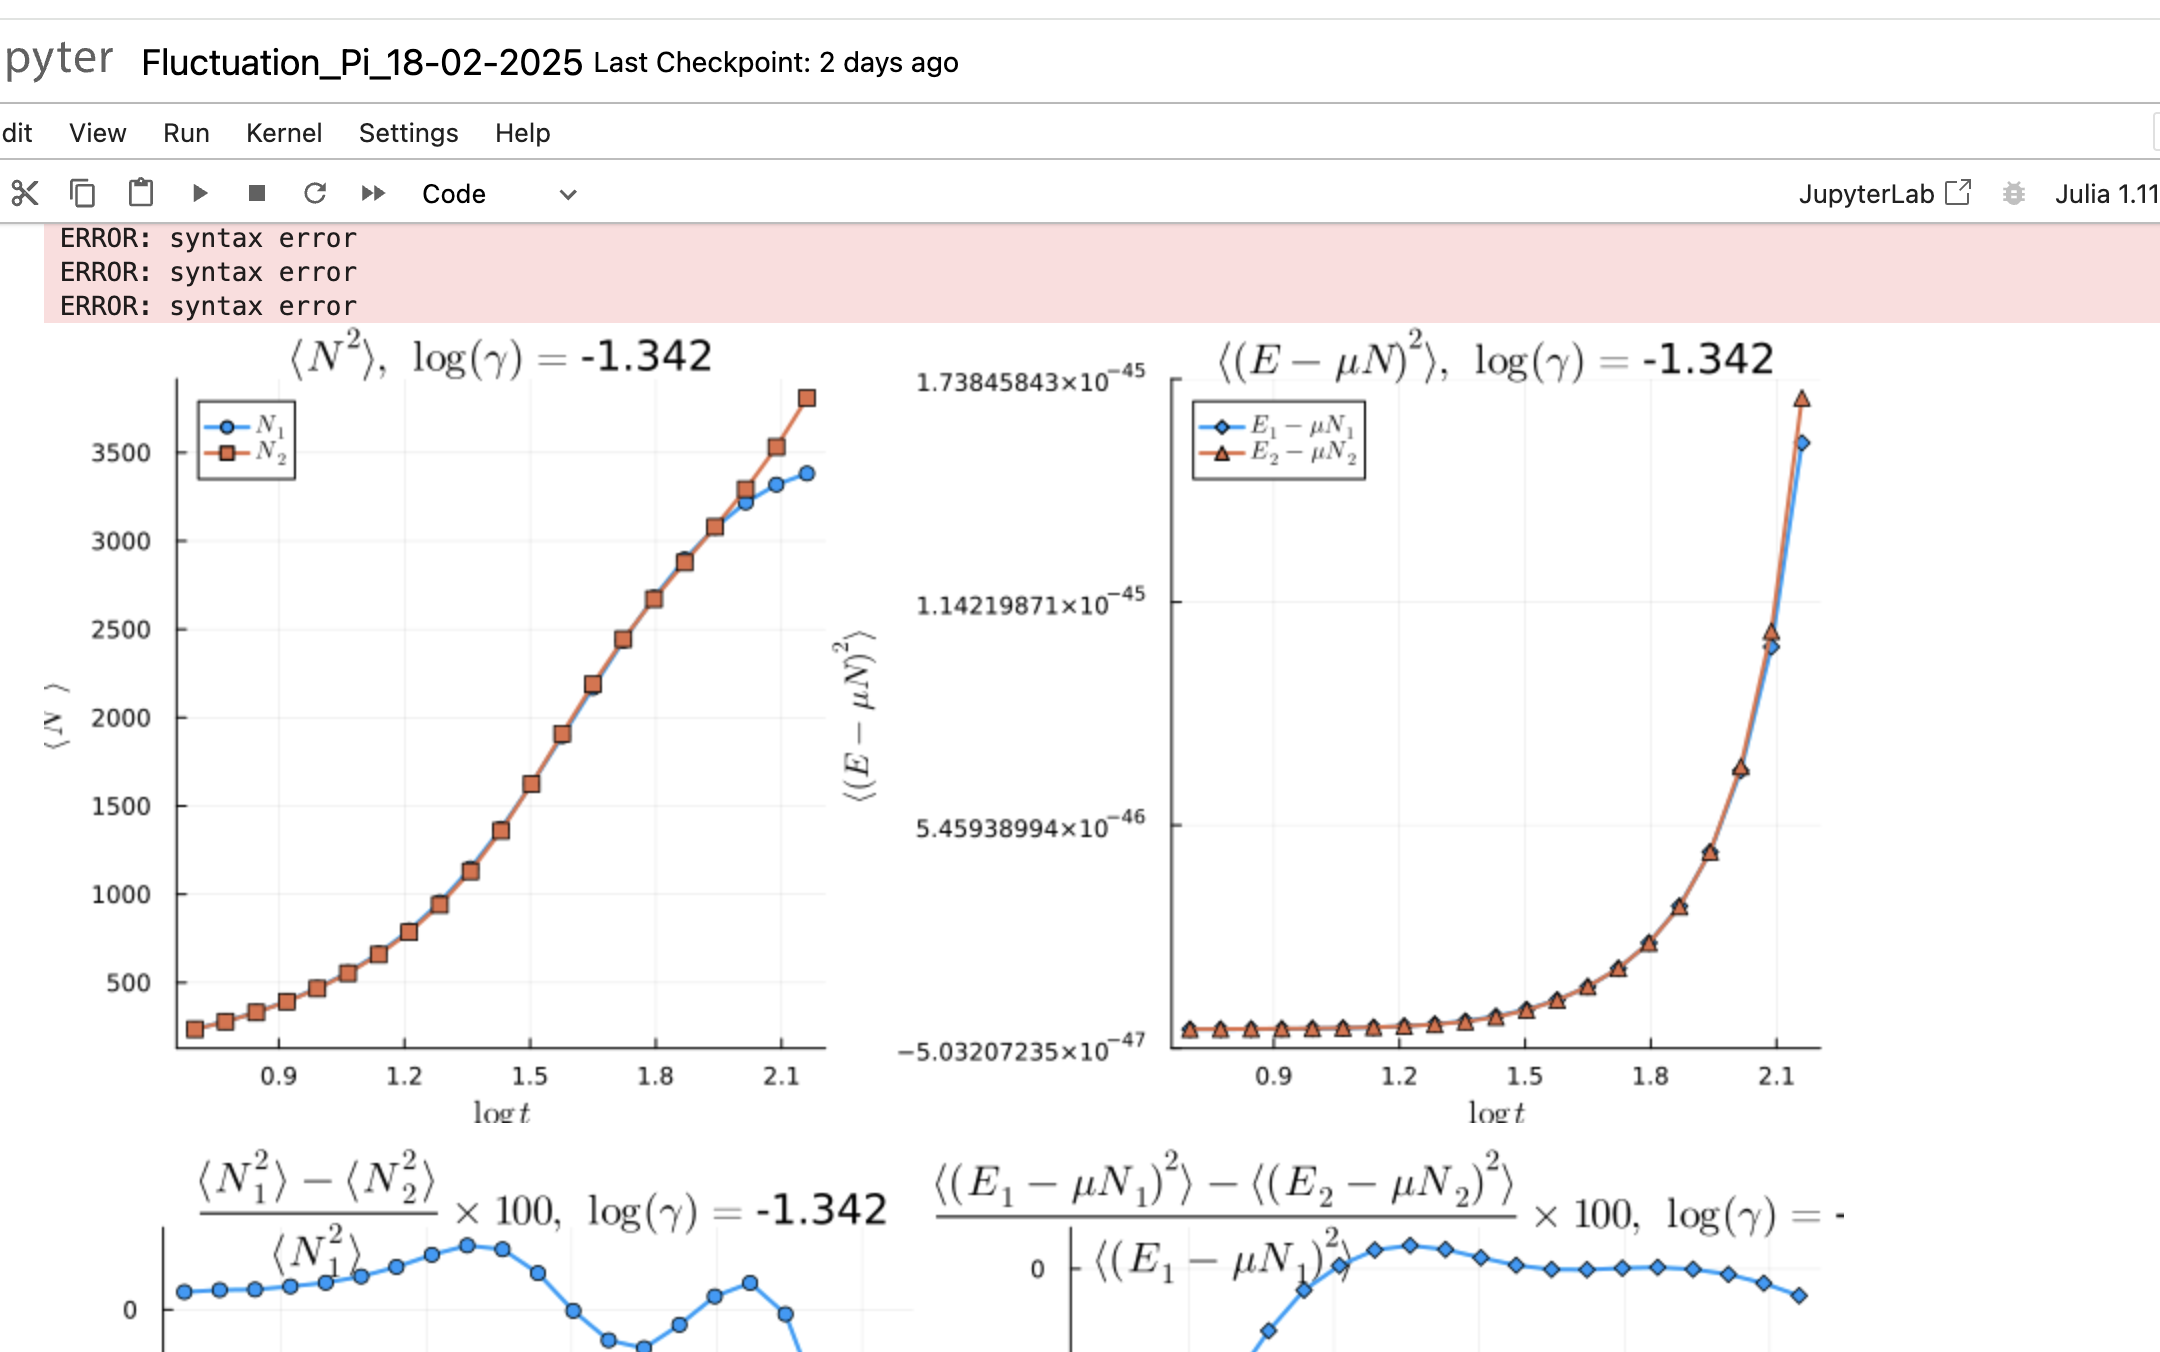
\includegraphics[width=1\textwidth]{Figures/test}

%\begin{aff}
%Donc une a l'ordre un en $\delta \theta (\operator{A}^{(0)})^{-1} %\operator{V}$ 

%\begin{eqnarray*}
%	\langle \delta \Pi ( \theta) \delta \Pi ( \theta') \rangle & = &  ( (\Pi^c_s - \Pi^c)\Pi^c/\Pi^c_s ) ( \theta ) \delta_{\theta, \theta'}/\delta \theta + \mathscr{F}(\theta , \theta' ) ,	
%\end{eqnarray*}

%avec 

%\begin{eqnarray*}
%	\mathscr{F}(\theta , \theta' ) & = & \left [ (\Pi^c_s - \Pi^c )( \theta)  +  (\Pi^c_s - \Pi^c ) ( \theta' )\right ] \frac{\Pi^c}{\Pi^c_s}(\theta)\frac{\Pi^c}{\Pi^c_s}(\theta') \frac{ \Delta( \theta'- \theta )}{ 2 \pi }\\
%	&&  - \left [ (\Pi^c_s - \Pi^c )( \theta)   (\Pi^c_s - \Pi^c ) ( \theta' )\right ] \frac{\Pi^c}{\Pi^c_s}(\theta)\frac{\Pi^c}{\Pi^c_s}(\theta')\int d\theta'' \left (   \frac{ \Pi^c/\Pi^c_s}{\Pi^c_s - \Pi^c} \right )(\theta'') \frac{\Delta(\theta''- \theta)}{2 \pi}\frac{\Delta(\theta''- \theta')}{2 \pi}  	
%\end{eqnarray*}
%\end{aff}



 









\subsection{Exemple : action de $\operator{P}$ sur l’état $\vert \psi_N\rangle$}
%Dans ce chapitre, nous nous intéressons aux fluctuations de la distribution de rapidité \( \delta \rho \) autour d'une distribution de référence \( \rho^c \), qui maximise la contribution à la fonction de partition des états, exprimée comme une fonctionnelle de la distribution \( \rho \) : 

La fonction de partition des états, s'exprime comme une fonctionnelle de la distribution \( \rho \) : 

\begin{eqnarray*}
	\Xi & = & \sum_\rho \exp \left( -\mathcal{A}(\rho) \right).
\end{eqnarray*}  

Dans la section {\em \bf Entropie de Yang-Yang} (\ref{??}), l'action \( \mathcal{A}(\rho) \) s'écrit sous la forme :  

\begin{eqnarray*}
	\mathcal{A}(\rho) & \doteq & - L\mathcal{S}_{YY}(\rho) + L\int f(\theta) \rho (\theta) \, d\theta,		
\end{eqnarray*}  

où \( \mathcal{S}_{YY} \) est la fonctionnelle d'entropie de Yang-Yang, définie dans (\ref{??}), et \( f \) est la fonction paramétrant les charges, introduite dans (\ref{??}).  

Dans cette même section {\em \bf Entropie de Yang-Yang} (\ref{??}), nous avons établi un lien entre \( f \) et distribution de référence \( \rho^c \), qui maximise la contribution à la fonction de partition des états .\\

On veux tester si nos experience est décrit pas un GGE. Pour cela nous nous intéressons aux fluctuations de la distribution de rapidité \( \delta \rho \) autour \( \rho^c \).

%Nous poursuivons à présent avec cette définition de l'action de classe $\mathcal{C}^2$ et admetant une distribution critique $\rho^c$ tel que sa différentielle en ce point critique soit nulle $d\mathcal{A}_{\rho^c} = 0 $ (\ref{??}) de sorte que d'aprés la formule de Taylor-Youg %afin de déterminer les fluctuations autour de \( \Pi^c \). Pour cela, nous réécrivons l'action sous la forme :  

Nous poursuivons à présent avec cette définition de l'action de classe $\mathcal{C}^2$ et admetant une distribution critique $\rho^c$ tel que sa différentielle en ce point critique soit nulle $d\mathcal{A}_{\rho^c} = 0 $ (\ref{??}) de sorte que d'aprés la formule de Taylor-Youg %afin de déterminer les fluctuations autour de \( \Pi^c \). Pour cela, nous réécrivons l'action sous la forme :  

\begin{eqnarray*}  
	\mathcal{A}(\rho^c + \delta \rho) & \underset{ \delta \rho \to 0 }{=} & \mathcal{A}(\rho^c)  + \frac{1}{2} \left. \frac{\delta^2 \mathcal{A}}{\delta \rho^2} \right|_{\rho^c} (\delta \rho) + \mathcal{O}((\delta \rho)^3),  
\end{eqnarray*}  

une expression quadratique pour l'action à l'ordre dominant en \( \delta \Pi \) avec $\left. \frac{\delta^2 \mathcal{A}}{\delta \rho^2} \right|_{\rho^c}$ la forme quadratique définie positive (Fig (\ref{fig.fluctu.A})).

\begin{figure}[H]
	\centering 
	\begin{tikzpicture}
		\begin{scope}[shift={(0,0)}]
			\begin{scope}[transform canvas={scale=0.6}]
				\input{Figures/Fonc_A_code}	
			
			\end{scope}
			
			\draw[color = red , scale = 0.5 , draw = none  ] (-2 , -1) rectangle (5, 6) ; 	
		\end{scope}
		
		\begin{scope}[shift={(19,-1)}]
			\begin{scope}[transform canvas={scale=0.6}]
				\input{Figures/Occupation_theta_code}	
			
			\end{scope}
			\begin{scope}[scale=1]
				\draw[color = red , scale = 1 , draw = none  ] (-1 , -1) rectangle (5, 5) ; 
			\end{scope}	
		\end{scope}

		
				
			
	\end{tikzpicture}	
	\captionsetup{skip=10pt} % Ajoute de l’espace après la légende
	\label{fig.fluctu.A}
\end{figure}


On discrétise l'axe des rapidités en  petite cellule de rapidité $[\theta, \theta+\delta\theta]$, qui contient $L\rho(\theta) \delta \theta$ rapidités. 
	



Avec ces petites tranches, la forme quadratique s’écrit :

\begin{eqnarray*}
    \left. \frac{\delta^2 \mathcal{A}}{{\delta \rho}^2} \right|_{\rho^c}(\delta \rho ) &=&  \sum_{a,b \mid \text{tranche}}  
    \delta \rho(\theta_a)  \frac{\partial^2 \mathcal{A}}{\partial \delta \rho(\theta_a) \partial \delta \rho(\theta_b) } (\rho^c)  \delta \rho(\theta_b).
\end{eqnarray*}
Les fluctuations s’écrivent donc :

\begin{eqnarray*}
    \langle \delta \rho ( \theta) \delta \rho ( \theta') \rangle &=&  
    \frac{ \int d\delta \rho \, \delta \rho(\theta) \delta \rho ( \theta') 
    \exp \left( - \frac{1}{2} \sum_{a,b \mid \text{tranche}}  
    \delta \rho(\theta_a) \frac{\partial^2 \mathcal{A}}{\partial \delta \rho(\theta_a) \partial \delta \rho(\theta_b) } (\rho^c)  \delta \rho(\theta_b) \right) }
    { \int d\delta \Pi  
    \exp \left( - \frac{1}{2} \sum_{a,b \mid \text{tranche}}  
    \delta \rho(\theta_a) \frac{\partial^2 \mathcal{A}}{\partial \delta \rho(\theta_a) \partial \delta \rho(\theta_b) } (\rho^c)  \delta \rho(\theta_b) \right) } \\
    &=& \left( \mathbf{A}^{-1} \right)_{\theta , \theta'}
\end{eqnarray*}


\begin{aff}

\begin{eqnarray*}
	\langle \delta \rho ( \theta) \delta \rho ( \theta') \rangle &=& 	\left( \mathbf{A}^{-1} \right)_{\theta , \theta'}
\end{eqnarray*}

	
avec la  {\em matrice hessienne} $\mathbf{A}_{\theta , \theta'} \equiv \frac{\partial^2 \mathcal{A}}{\partial \delta \rho(\theta) \partial \delta \rho(\theta') }(\rho^c)$, au point critique/ qui maximise la probabilité  $\rho^c=\rho^c_s \nu^c $, s'écrit

\begin{eqnarray*}
	\operator{A} & = & \operator{A}^{(0)} + \delta \theta \operator{V}
\end{eqnarray*}

avec 

\begin{eqnarray*}
	A^{(0)}_{\theta , \theta'}  & = &  L\delta \theta \left ( \frac{ 1}{\rho^c_s ( 1  - \nu^c ) \nu^c } \right )(\theta)    \delta({\theta - \theta '})	,\\
	V_{\theta , \theta'}  &= & L \delta \theta \left \{ - \left [ \left ( \frac{1}{\rho^c_s( 1 - \nu^c) } \right ) ( \theta)  +  \left ( \frac{1}{\rho^c_s( 1 - \nu^c) } \right ) ( \theta' )\right ] \frac{ \Delta( \theta'- \theta )}{ 2 \pi } + \int d\theta''  \left ( \frac{\nu^c}{\rho^c_s( 1 - \nu^c) } \right )(\theta'') \frac{\Delta(\theta''- \theta)}{2 \pi}\frac{\Delta(\theta''- \theta')}{2 \pi}   \right \} 	
\end{eqnarray*}

\end{aff}

\subsection{Testes}

\begin{eqnarray*}
	\Delta_{\operator{\mathcal{N}}}^2  & = &  \frac{1}{\beta} \left . \frac{\partial \langle \operator{\mathcal{N}} \rangle}{\partial \mu} \right )_T \\
	\Delta_{\operator{\mathcal{E}}-\mu \operator{\mathcal{N}}}^2  & = &  - \left . \frac{\partial \langle \operator{\mathcal{E}}-\mu \operator{\mathcal{N}} \rangle}{\partial \beta} \right )_\mu 
\end{eqnarray*}

et 

\begin{eqnarray*}
	\Delta_{\operator{\mathcal{N}}}^2  &= & L^2 \int d\theta_a \int d \theta_b \, \langle \delta \rho(\theta_a) \delta \rho(\theta_b) \rangle \\
	\Delta_{\operator{\mathcal{E}}-\mu \operator{\mathcal{N}}}^2  & = & L^2 \int d\theta_a \int d \theta_b \, \left ( - \mu + \frac{1}2 m \theta_a^2  \right  )\left ( - \mu + \frac{1}2 m \theta_b^2  \right  )  \langle \delta \rho(\theta_a) \delta \rho(\theta_b) \rangle
\end{eqnarray*}

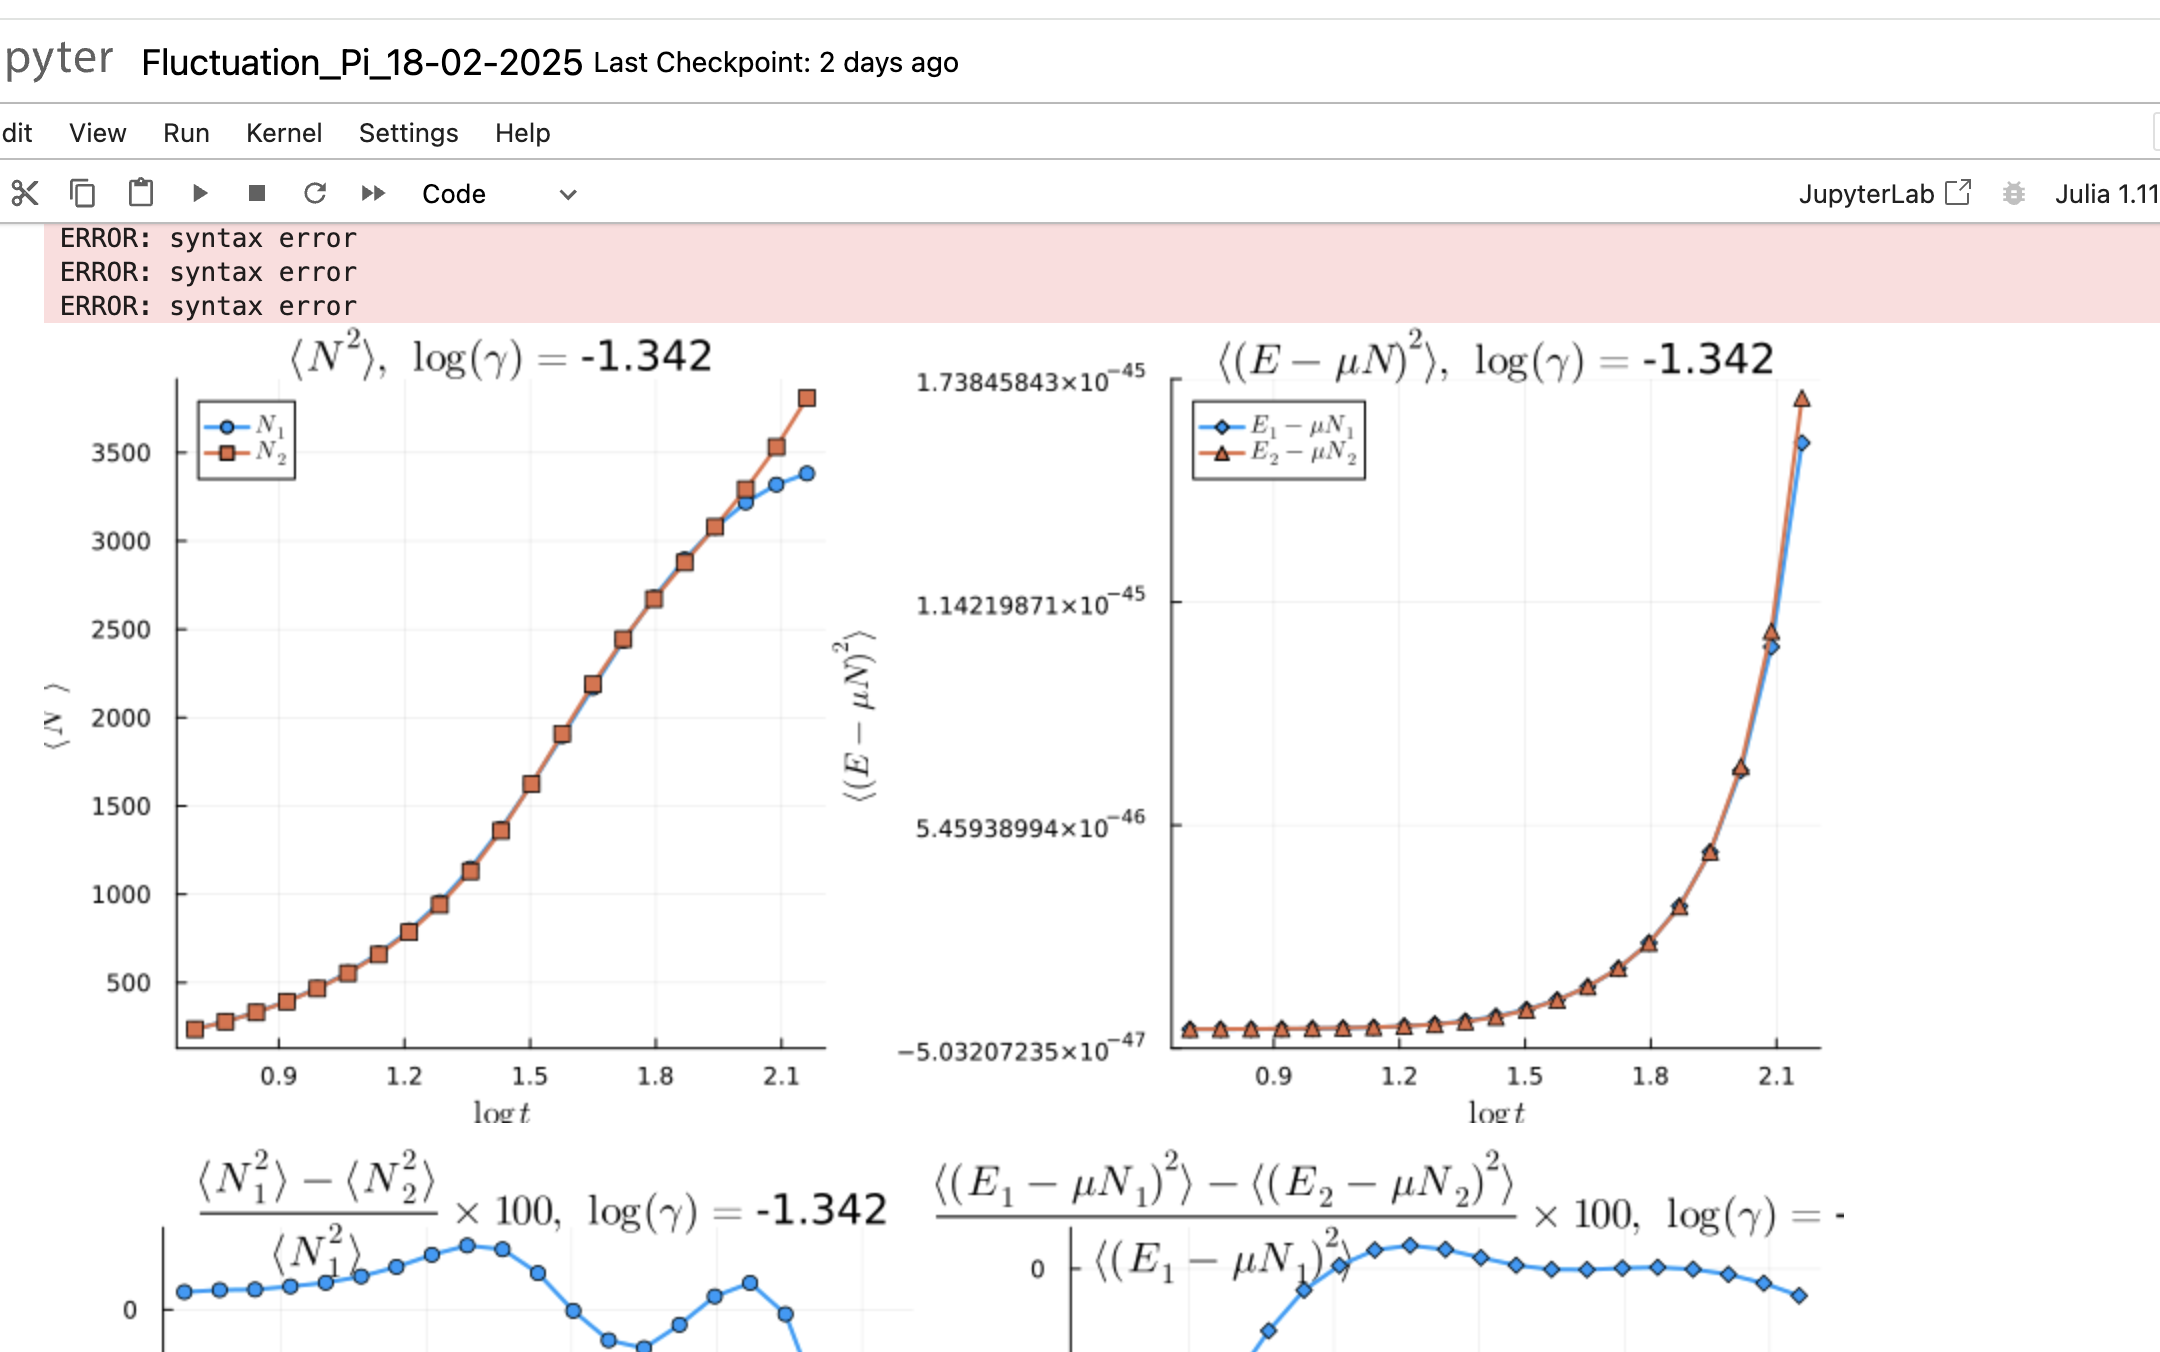
\includegraphics[width=1\textwidth]{Figures/test}

%\begin{aff}
%Donc une a l'ordre un en $\delta \theta (\operator{A}^{(0)})^{-1} %\operator{V}$ 

%\begin{eqnarray*}
%	\langle \delta \Pi ( \theta) \delta \Pi ( \theta') \rangle & = &  ( (\Pi^c_s - \Pi^c)\Pi^c/\Pi^c_s ) ( \theta ) \delta_{\theta, \theta'}/\delta \theta + \mathscr{F}(\theta , \theta' ) ,	
%\end{eqnarray*}

%avec 

%\begin{eqnarray*}
%	\mathscr{F}(\theta , \theta' ) & = & \left [ (\Pi^c_s - \Pi^c )( \theta)  +  (\Pi^c_s - \Pi^c ) ( \theta' )\right ] \frac{\Pi^c}{\Pi^c_s}(\theta)\frac{\Pi^c}{\Pi^c_s}(\theta') \frac{ \Delta( \theta'- \theta )}{ 2 \pi }\\
%	&&  - \left [ (\Pi^c_s - \Pi^c )( \theta)   (\Pi^c_s - \Pi^c ) ( \theta' )\right ] \frac{\Pi^c}{\Pi^c_s}(\theta)\frac{\Pi^c}{\Pi^c_s}(\theta')\int d\theta'' \left (   \frac{ \Pi^c/\Pi^c_s}{\Pi^c_s - \Pi^c} \right )(\theta'') \frac{\Delta(\theta''- \theta)}{2 \pi}\frac{\Delta(\theta''- \theta')}{2 \pi}  	
%\end{eqnarray*}
%\end{aff}



 









\subsection{Aaction de $\operator{H}$ sur l’état $\vert \psi_N\rangle$}
%Dans ce chapitre, nous nous intéressons aux fluctuations de la distribution de rapidité \( \delta \rho \) autour d'une distribution de référence \( \rho^c \), qui maximise la contribution à la fonction de partition des états, exprimée comme une fonctionnelle de la distribution \( \rho \) : 

La fonction de partition des états, s'exprime comme une fonctionnelle de la distribution \( \rho \) : 

\begin{eqnarray*}
	\Xi & = & \sum_\rho \exp \left( -\mathcal{A}(\rho) \right).
\end{eqnarray*}  

Dans la section {\em \bf Entropie de Yang-Yang} (\ref{??}), l'action \( \mathcal{A}(\rho) \) s'écrit sous la forme :  

\begin{eqnarray*}
	\mathcal{A}(\rho) & \doteq & - L\mathcal{S}_{YY}(\rho) + L\int f(\theta) \rho (\theta) \, d\theta,		
\end{eqnarray*}  

où \( \mathcal{S}_{YY} \) est la fonctionnelle d'entropie de Yang-Yang, définie dans (\ref{??}), et \( f \) est la fonction paramétrant les charges, introduite dans (\ref{??}).  

Dans cette même section {\em \bf Entropie de Yang-Yang} (\ref{??}), nous avons établi un lien entre \( f \) et distribution de référence \( \rho^c \), qui maximise la contribution à la fonction de partition des états .\\

On veux tester si nos experience est décrit pas un GGE. Pour cela nous nous intéressons aux fluctuations de la distribution de rapidité \( \delta \rho \) autour \( \rho^c \).

%Nous poursuivons à présent avec cette définition de l'action de classe $\mathcal{C}^2$ et admetant une distribution critique $\rho^c$ tel que sa différentielle en ce point critique soit nulle $d\mathcal{A}_{\rho^c} = 0 $ (\ref{??}) de sorte que d'aprés la formule de Taylor-Youg %afin de déterminer les fluctuations autour de \( \Pi^c \). Pour cela, nous réécrivons l'action sous la forme :  

Nous poursuivons à présent avec cette définition de l'action de classe $\mathcal{C}^2$ et admetant une distribution critique $\rho^c$ tel que sa différentielle en ce point critique soit nulle $d\mathcal{A}_{\rho^c} = 0 $ (\ref{??}) de sorte que d'aprés la formule de Taylor-Youg %afin de déterminer les fluctuations autour de \( \Pi^c \). Pour cela, nous réécrivons l'action sous la forme :  

\begin{eqnarray*}  
	\mathcal{A}(\rho^c + \delta \rho) & \underset{ \delta \rho \to 0 }{=} & \mathcal{A}(\rho^c)  + \frac{1}{2} \left. \frac{\delta^2 \mathcal{A}}{\delta \rho^2} \right|_{\rho^c} (\delta \rho) + \mathcal{O}((\delta \rho)^3),  
\end{eqnarray*}  

une expression quadratique pour l'action à l'ordre dominant en \( \delta \Pi \) avec $\left. \frac{\delta^2 \mathcal{A}}{\delta \rho^2} \right|_{\rho^c}$ la forme quadratique définie positive (Fig (\ref{fig.fluctu.A})).

\begin{figure}[H]
	\centering 
	\begin{tikzpicture}
		\begin{scope}[shift={(0,0)}]
			\begin{scope}[transform canvas={scale=0.6}]
				\input{Figures/Fonc_A_code}	
			
			\end{scope}
			
			\draw[color = red , scale = 0.5 , draw = none  ] (-2 , -1) rectangle (5, 6) ; 	
		\end{scope}
		
		\begin{scope}[shift={(19,-1)}]
			\begin{scope}[transform canvas={scale=0.6}]
				\input{Figures/Occupation_theta_code}	
			
			\end{scope}
			\begin{scope}[scale=1]
				\draw[color = red , scale = 1 , draw = none  ] (-1 , -1) rectangle (5, 5) ; 
			\end{scope}	
		\end{scope}

		
				
			
	\end{tikzpicture}	
	\captionsetup{skip=10pt} % Ajoute de l’espace après la légende
	\label{fig.fluctu.A}
\end{figure}


On discrétise l'axe des rapidités en  petite cellule de rapidité $[\theta, \theta+\delta\theta]$, qui contient $L\rho(\theta) \delta \theta$ rapidités. 
	



Avec ces petites tranches, la forme quadratique s’écrit :

\begin{eqnarray*}
    \left. \frac{\delta^2 \mathcal{A}}{{\delta \rho}^2} \right|_{\rho^c}(\delta \rho ) &=&  \sum_{a,b \mid \text{tranche}}  
    \delta \rho(\theta_a)  \frac{\partial^2 \mathcal{A}}{\partial \delta \rho(\theta_a) \partial \delta \rho(\theta_b) } (\rho^c)  \delta \rho(\theta_b).
\end{eqnarray*}
Les fluctuations s’écrivent donc :

\begin{eqnarray*}
    \langle \delta \rho ( \theta) \delta \rho ( \theta') \rangle &=&  
    \frac{ \int d\delta \rho \, \delta \rho(\theta) \delta \rho ( \theta') 
    \exp \left( - \frac{1}{2} \sum_{a,b \mid \text{tranche}}  
    \delta \rho(\theta_a) \frac{\partial^2 \mathcal{A}}{\partial \delta \rho(\theta_a) \partial \delta \rho(\theta_b) } (\rho^c)  \delta \rho(\theta_b) \right) }
    { \int d\delta \Pi  
    \exp \left( - \frac{1}{2} \sum_{a,b \mid \text{tranche}}  
    \delta \rho(\theta_a) \frac{\partial^2 \mathcal{A}}{\partial \delta \rho(\theta_a) \partial \delta \rho(\theta_b) } (\rho^c)  \delta \rho(\theta_b) \right) } \\
    &=& \left( \mathbf{A}^{-1} \right)_{\theta , \theta'}
\end{eqnarray*}


\begin{aff}

\begin{eqnarray*}
	\langle \delta \rho ( \theta) \delta \rho ( \theta') \rangle &=& 	\left( \mathbf{A}^{-1} \right)_{\theta , \theta'}
\end{eqnarray*}

	
avec la  {\em matrice hessienne} $\mathbf{A}_{\theta , \theta'} \equiv \frac{\partial^2 \mathcal{A}}{\partial \delta \rho(\theta) \partial \delta \rho(\theta') }(\rho^c)$, au point critique/ qui maximise la probabilité  $\rho^c=\rho^c_s \nu^c $, s'écrit

\begin{eqnarray*}
	\operator{A} & = & \operator{A}^{(0)} + \delta \theta \operator{V}
\end{eqnarray*}

avec 

\begin{eqnarray*}
	A^{(0)}_{\theta , \theta'}  & = &  L\delta \theta \left ( \frac{ 1}{\rho^c_s ( 1  - \nu^c ) \nu^c } \right )(\theta)    \delta({\theta - \theta '})	,\\
	V_{\theta , \theta'}  &= & L \delta \theta \left \{ - \left [ \left ( \frac{1}{\rho^c_s( 1 - \nu^c) } \right ) ( \theta)  +  \left ( \frac{1}{\rho^c_s( 1 - \nu^c) } \right ) ( \theta' )\right ] \frac{ \Delta( \theta'- \theta )}{ 2 \pi } + \int d\theta''  \left ( \frac{\nu^c}{\rho^c_s( 1 - \nu^c) } \right )(\theta'') \frac{\Delta(\theta''- \theta)}{2 \pi}\frac{\Delta(\theta''- \theta')}{2 \pi}   \right \} 	
\end{eqnarray*}

\end{aff}

\subsection{Testes}

\begin{eqnarray*}
	\Delta_{\operator{\mathcal{N}}}^2  & = &  \frac{1}{\beta} \left . \frac{\partial \langle \operator{\mathcal{N}} \rangle}{\partial \mu} \right )_T \\
	\Delta_{\operator{\mathcal{E}}-\mu \operator{\mathcal{N}}}^2  & = &  - \left . \frac{\partial \langle \operator{\mathcal{E}}-\mu \operator{\mathcal{N}} \rangle}{\partial \beta} \right )_\mu 
\end{eqnarray*}

et 

\begin{eqnarray*}
	\Delta_{\operator{\mathcal{N}}}^2  &= & L^2 \int d\theta_a \int d \theta_b \, \langle \delta \rho(\theta_a) \delta \rho(\theta_b) \rangle \\
	\Delta_{\operator{\mathcal{E}}-\mu \operator{\mathcal{N}}}^2  & = & L^2 \int d\theta_a \int d \theta_b \, \left ( - \mu + \frac{1}2 m \theta_a^2  \right  )\left ( - \mu + \frac{1}2 m \theta_b^2  \right  )  \langle \delta \rho(\theta_a) \delta \rho(\theta_b) \rangle
\end{eqnarray*}

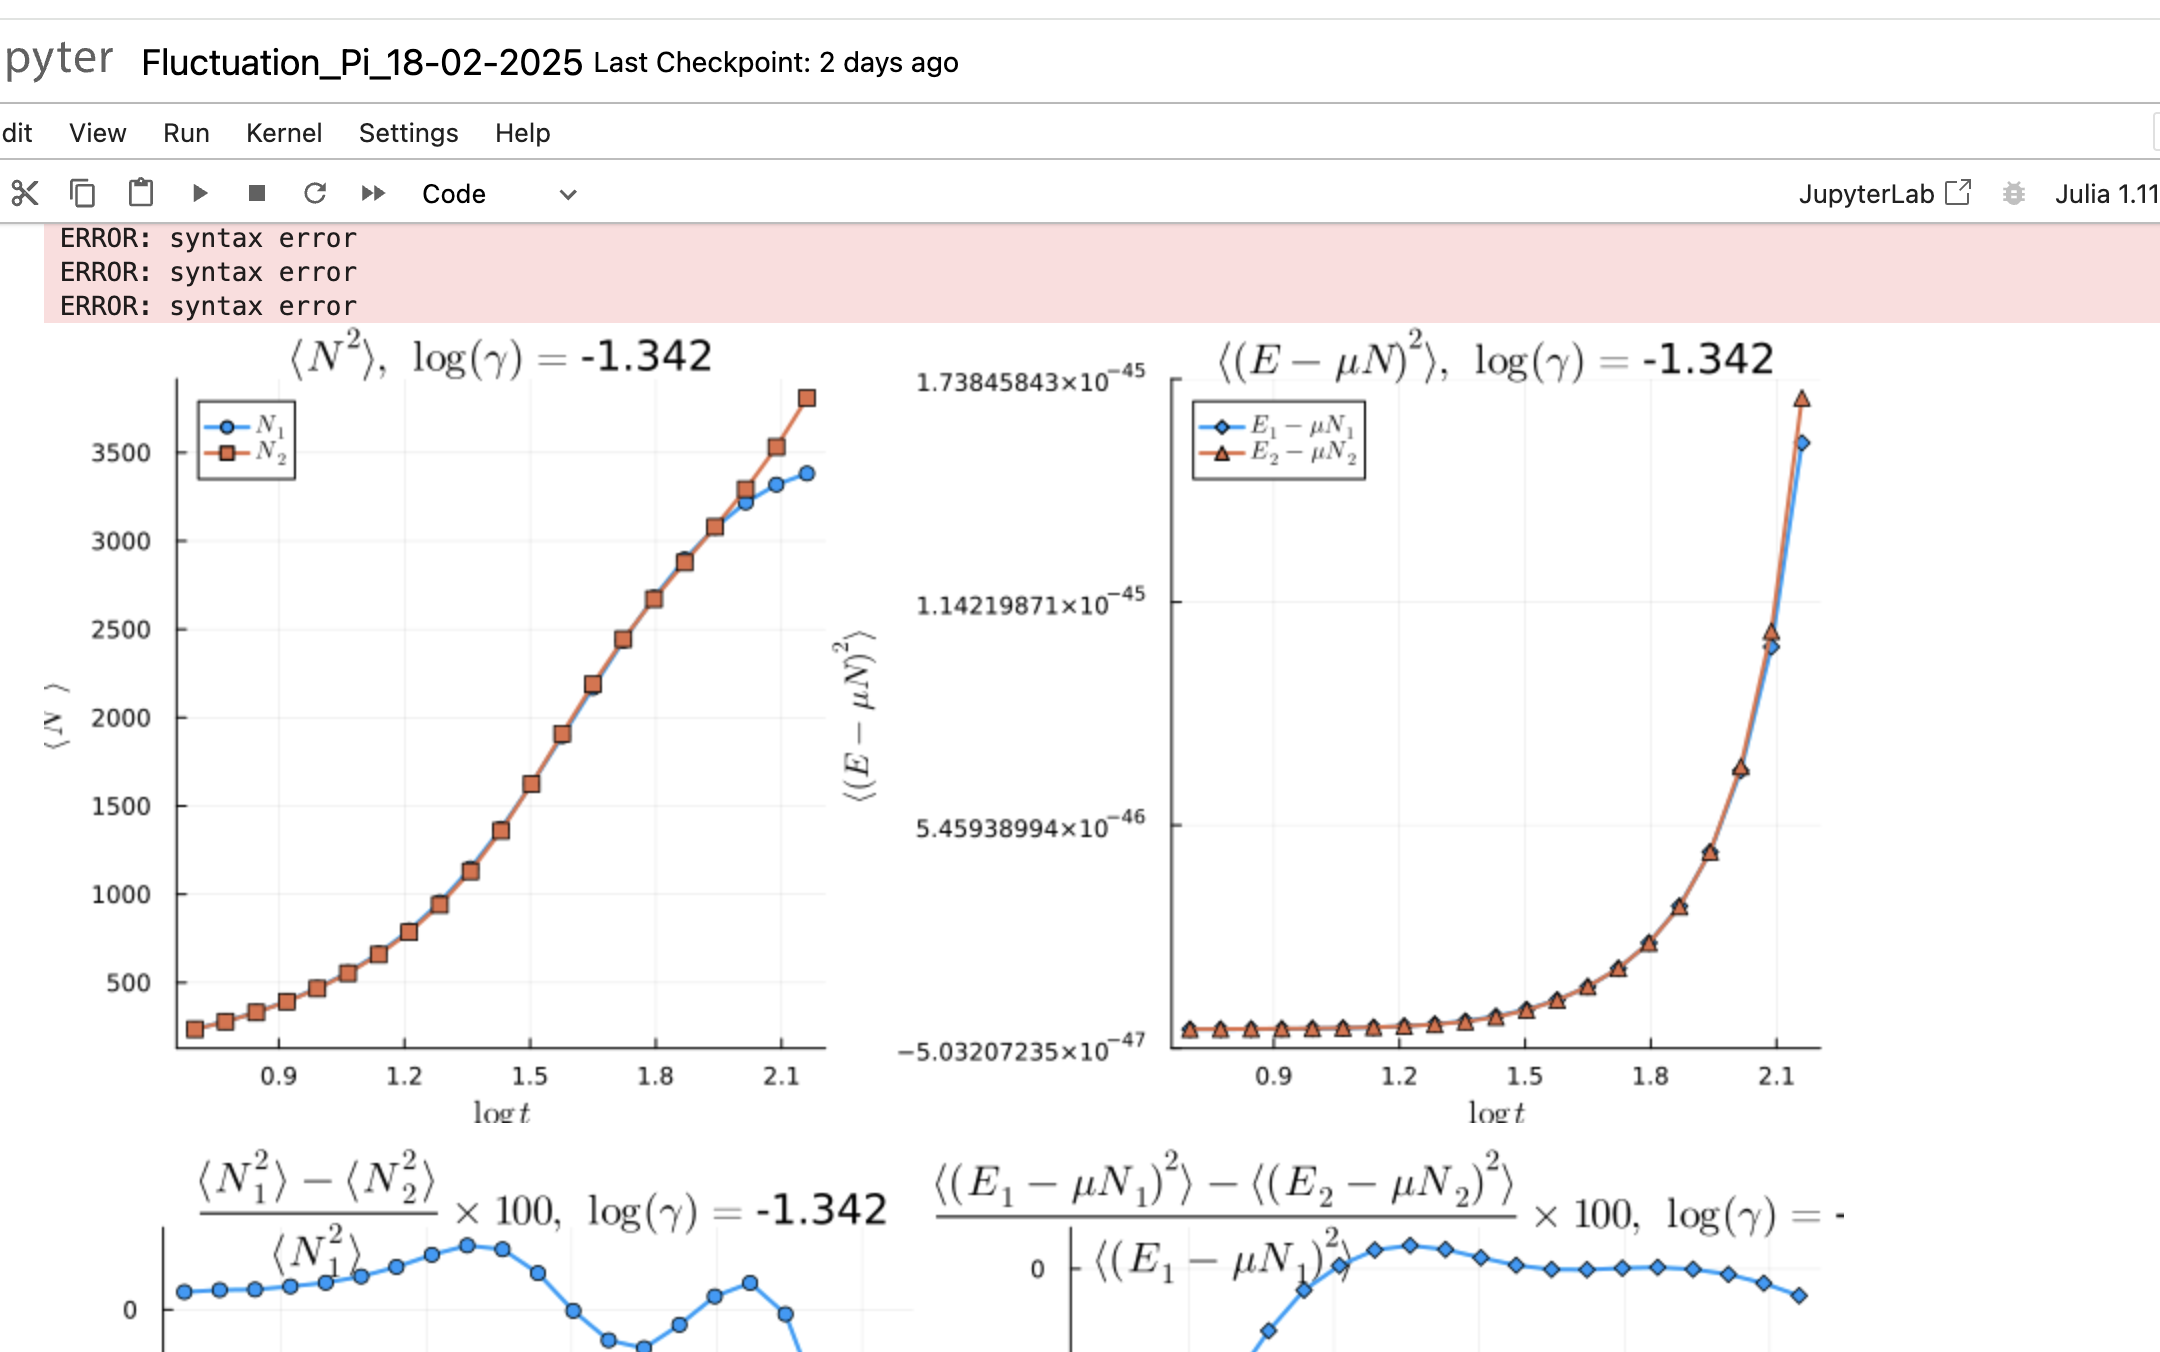
\includegraphics[width=1\textwidth]{Figures/test}

%\begin{aff}
%Donc une a l'ordre un en $\delta \theta (\operator{A}^{(0)})^{-1} %\operator{V}$ 

%\begin{eqnarray*}
%	\langle \delta \Pi ( \theta) \delta \Pi ( \theta') \rangle & = &  ( (\Pi^c_s - \Pi^c)\Pi^c/\Pi^c_s ) ( \theta ) \delta_{\theta, \theta'}/\delta \theta + \mathscr{F}(\theta , \theta' ) ,	
%\end{eqnarray*}

%avec 

%\begin{eqnarray*}
%	\mathscr{F}(\theta , \theta' ) & = & \left [ (\Pi^c_s - \Pi^c )( \theta)  +  (\Pi^c_s - \Pi^c ) ( \theta' )\right ] \frac{\Pi^c}{\Pi^c_s}(\theta)\frac{\Pi^c}{\Pi^c_s}(\theta') \frac{ \Delta( \theta'- \theta )}{ 2 \pi }\\
%	&&  - \left [ (\Pi^c_s - \Pi^c )( \theta)   (\Pi^c_s - \Pi^c ) ( \theta' )\right ] \frac{\Pi^c}{\Pi^c_s}(\theta)\frac{\Pi^c}{\Pi^c_s}(\theta')\int d\theta'' \left (   \frac{ \Pi^c/\Pi^c_s}{\Pi^c_s - \Pi^c} \right )(\theta'') \frac{\Delta(\theta''- \theta)}{2 \pi}\frac{\Delta(\theta''- \theta')}{2 \pi}  	
%\end{eqnarray*}
%\end{aff}



 









\subsection{Vérification explicite de la condition aux limites}
%Dans ce chapitre, nous nous intéressons aux fluctuations de la distribution de rapidité \( \delta \rho \) autour d'une distribution de référence \( \rho^c \), qui maximise la contribution à la fonction de partition des états, exprimée comme une fonctionnelle de la distribution \( \rho \) : 

La fonction de partition des états, s'exprime comme une fonctionnelle de la distribution \( \rho \) : 

\begin{eqnarray*}
	\Xi & = & \sum_\rho \exp \left( -\mathcal{A}(\rho) \right).
\end{eqnarray*}  

Dans la section {\em \bf Entropie de Yang-Yang} (\ref{??}), l'action \( \mathcal{A}(\rho) \) s'écrit sous la forme :  

\begin{eqnarray*}
	\mathcal{A}(\rho) & \doteq & - L\mathcal{S}_{YY}(\rho) + L\int f(\theta) \rho (\theta) \, d\theta,		
\end{eqnarray*}  

où \( \mathcal{S}_{YY} \) est la fonctionnelle d'entropie de Yang-Yang, définie dans (\ref{??}), et \( f \) est la fonction paramétrant les charges, introduite dans (\ref{??}).  

Dans cette même section {\em \bf Entropie de Yang-Yang} (\ref{??}), nous avons établi un lien entre \( f \) et distribution de référence \( \rho^c \), qui maximise la contribution à la fonction de partition des états .\\

On veux tester si nos experience est décrit pas un GGE. Pour cela nous nous intéressons aux fluctuations de la distribution de rapidité \( \delta \rho \) autour \( \rho^c \).

%Nous poursuivons à présent avec cette définition de l'action de classe $\mathcal{C}^2$ et admetant une distribution critique $\rho^c$ tel que sa différentielle en ce point critique soit nulle $d\mathcal{A}_{\rho^c} = 0 $ (\ref{??}) de sorte que d'aprés la formule de Taylor-Youg %afin de déterminer les fluctuations autour de \( \Pi^c \). Pour cela, nous réécrivons l'action sous la forme :  

Nous poursuivons à présent avec cette définition de l'action de classe $\mathcal{C}^2$ et admetant une distribution critique $\rho^c$ tel que sa différentielle en ce point critique soit nulle $d\mathcal{A}_{\rho^c} = 0 $ (\ref{??}) de sorte que d'aprés la formule de Taylor-Youg %afin de déterminer les fluctuations autour de \( \Pi^c \). Pour cela, nous réécrivons l'action sous la forme :  

\begin{eqnarray*}  
	\mathcal{A}(\rho^c + \delta \rho) & \underset{ \delta \rho \to 0 }{=} & \mathcal{A}(\rho^c)  + \frac{1}{2} \left. \frac{\delta^2 \mathcal{A}}{\delta \rho^2} \right|_{\rho^c} (\delta \rho) + \mathcal{O}((\delta \rho)^3),  
\end{eqnarray*}  

une expression quadratique pour l'action à l'ordre dominant en \( \delta \Pi \) avec $\left. \frac{\delta^2 \mathcal{A}}{\delta \rho^2} \right|_{\rho^c}$ la forme quadratique définie positive (Fig (\ref{fig.fluctu.A})).

\begin{figure}[H]
	\centering 
	\begin{tikzpicture}
		\begin{scope}[shift={(0,0)}]
			\begin{scope}[transform canvas={scale=0.6}]
				\input{Figures/Fonc_A_code}	
			
			\end{scope}
			
			\draw[color = red , scale = 0.5 , draw = none  ] (-2 , -1) rectangle (5, 6) ; 	
		\end{scope}
		
		\begin{scope}[shift={(19,-1)}]
			\begin{scope}[transform canvas={scale=0.6}]
				\input{Figures/Occupation_theta_code}	
			
			\end{scope}
			\begin{scope}[scale=1]
				\draw[color = red , scale = 1 , draw = none  ] (-1 , -1) rectangle (5, 5) ; 
			\end{scope}	
		\end{scope}

		
				
			
	\end{tikzpicture}	
	\captionsetup{skip=10pt} % Ajoute de l’espace après la légende
	\label{fig.fluctu.A}
\end{figure}


On discrétise l'axe des rapidités en  petite cellule de rapidité $[\theta, \theta+\delta\theta]$, qui contient $L\rho(\theta) \delta \theta$ rapidités. 
	



Avec ces petites tranches, la forme quadratique s’écrit :

\begin{eqnarray*}
    \left. \frac{\delta^2 \mathcal{A}}{{\delta \rho}^2} \right|_{\rho^c}(\delta \rho ) &=&  \sum_{a,b \mid \text{tranche}}  
    \delta \rho(\theta_a)  \frac{\partial^2 \mathcal{A}}{\partial \delta \rho(\theta_a) \partial \delta \rho(\theta_b) } (\rho^c)  \delta \rho(\theta_b).
\end{eqnarray*}
Les fluctuations s’écrivent donc :

\begin{eqnarray*}
    \langle \delta \rho ( \theta) \delta \rho ( \theta') \rangle &=&  
    \frac{ \int d\delta \rho \, \delta \rho(\theta) \delta \rho ( \theta') 
    \exp \left( - \frac{1}{2} \sum_{a,b \mid \text{tranche}}  
    \delta \rho(\theta_a) \frac{\partial^2 \mathcal{A}}{\partial \delta \rho(\theta_a) \partial \delta \rho(\theta_b) } (\rho^c)  \delta \rho(\theta_b) \right) }
    { \int d\delta \Pi  
    \exp \left( - \frac{1}{2} \sum_{a,b \mid \text{tranche}}  
    \delta \rho(\theta_a) \frac{\partial^2 \mathcal{A}}{\partial \delta \rho(\theta_a) \partial \delta \rho(\theta_b) } (\rho^c)  \delta \rho(\theta_b) \right) } \\
    &=& \left( \mathbf{A}^{-1} \right)_{\theta , \theta'}
\end{eqnarray*}


\begin{aff}

\begin{eqnarray*}
	\langle \delta \rho ( \theta) \delta \rho ( \theta') \rangle &=& 	\left( \mathbf{A}^{-1} \right)_{\theta , \theta'}
\end{eqnarray*}

	
avec la  {\em matrice hessienne} $\mathbf{A}_{\theta , \theta'} \equiv \frac{\partial^2 \mathcal{A}}{\partial \delta \rho(\theta) \partial \delta \rho(\theta') }(\rho^c)$, au point critique/ qui maximise la probabilité  $\rho^c=\rho^c_s \nu^c $, s'écrit

\begin{eqnarray*}
	\operator{A} & = & \operator{A}^{(0)} + \delta \theta \operator{V}
\end{eqnarray*}

avec 

\begin{eqnarray*}
	A^{(0)}_{\theta , \theta'}  & = &  L\delta \theta \left ( \frac{ 1}{\rho^c_s ( 1  - \nu^c ) \nu^c } \right )(\theta)    \delta({\theta - \theta '})	,\\
	V_{\theta , \theta'}  &= & L \delta \theta \left \{ - \left [ \left ( \frac{1}{\rho^c_s( 1 - \nu^c) } \right ) ( \theta)  +  \left ( \frac{1}{\rho^c_s( 1 - \nu^c) } \right ) ( \theta' )\right ] \frac{ \Delta( \theta'- \theta )}{ 2 \pi } + \int d\theta''  \left ( \frac{\nu^c}{\rho^c_s( 1 - \nu^c) } \right )(\theta'') \frac{\Delta(\theta''- \theta)}{2 \pi}\frac{\Delta(\theta''- \theta')}{2 \pi}   \right \} 	
\end{eqnarray*}

\end{aff}

\subsection{Testes}

\begin{eqnarray*}
	\Delta_{\operator{\mathcal{N}}}^2  & = &  \frac{1}{\beta} \left . \frac{\partial \langle \operator{\mathcal{N}} \rangle}{\partial \mu} \right )_T \\
	\Delta_{\operator{\mathcal{E}}-\mu \operator{\mathcal{N}}}^2  & = &  - \left . \frac{\partial \langle \operator{\mathcal{E}}-\mu \operator{\mathcal{N}} \rangle}{\partial \beta} \right )_\mu 
\end{eqnarray*}

et 

\begin{eqnarray*}
	\Delta_{\operator{\mathcal{N}}}^2  &= & L^2 \int d\theta_a \int d \theta_b \, \langle \delta \rho(\theta_a) \delta \rho(\theta_b) \rangle \\
	\Delta_{\operator{\mathcal{E}}-\mu \operator{\mathcal{N}}}^2  & = & L^2 \int d\theta_a \int d \theta_b \, \left ( - \mu + \frac{1}2 m \theta_a^2  \right  )\left ( - \mu + \frac{1}2 m \theta_b^2  \right  )  \langle \delta \rho(\theta_a) \delta \rho(\theta_b) \rangle
\end{eqnarray*}

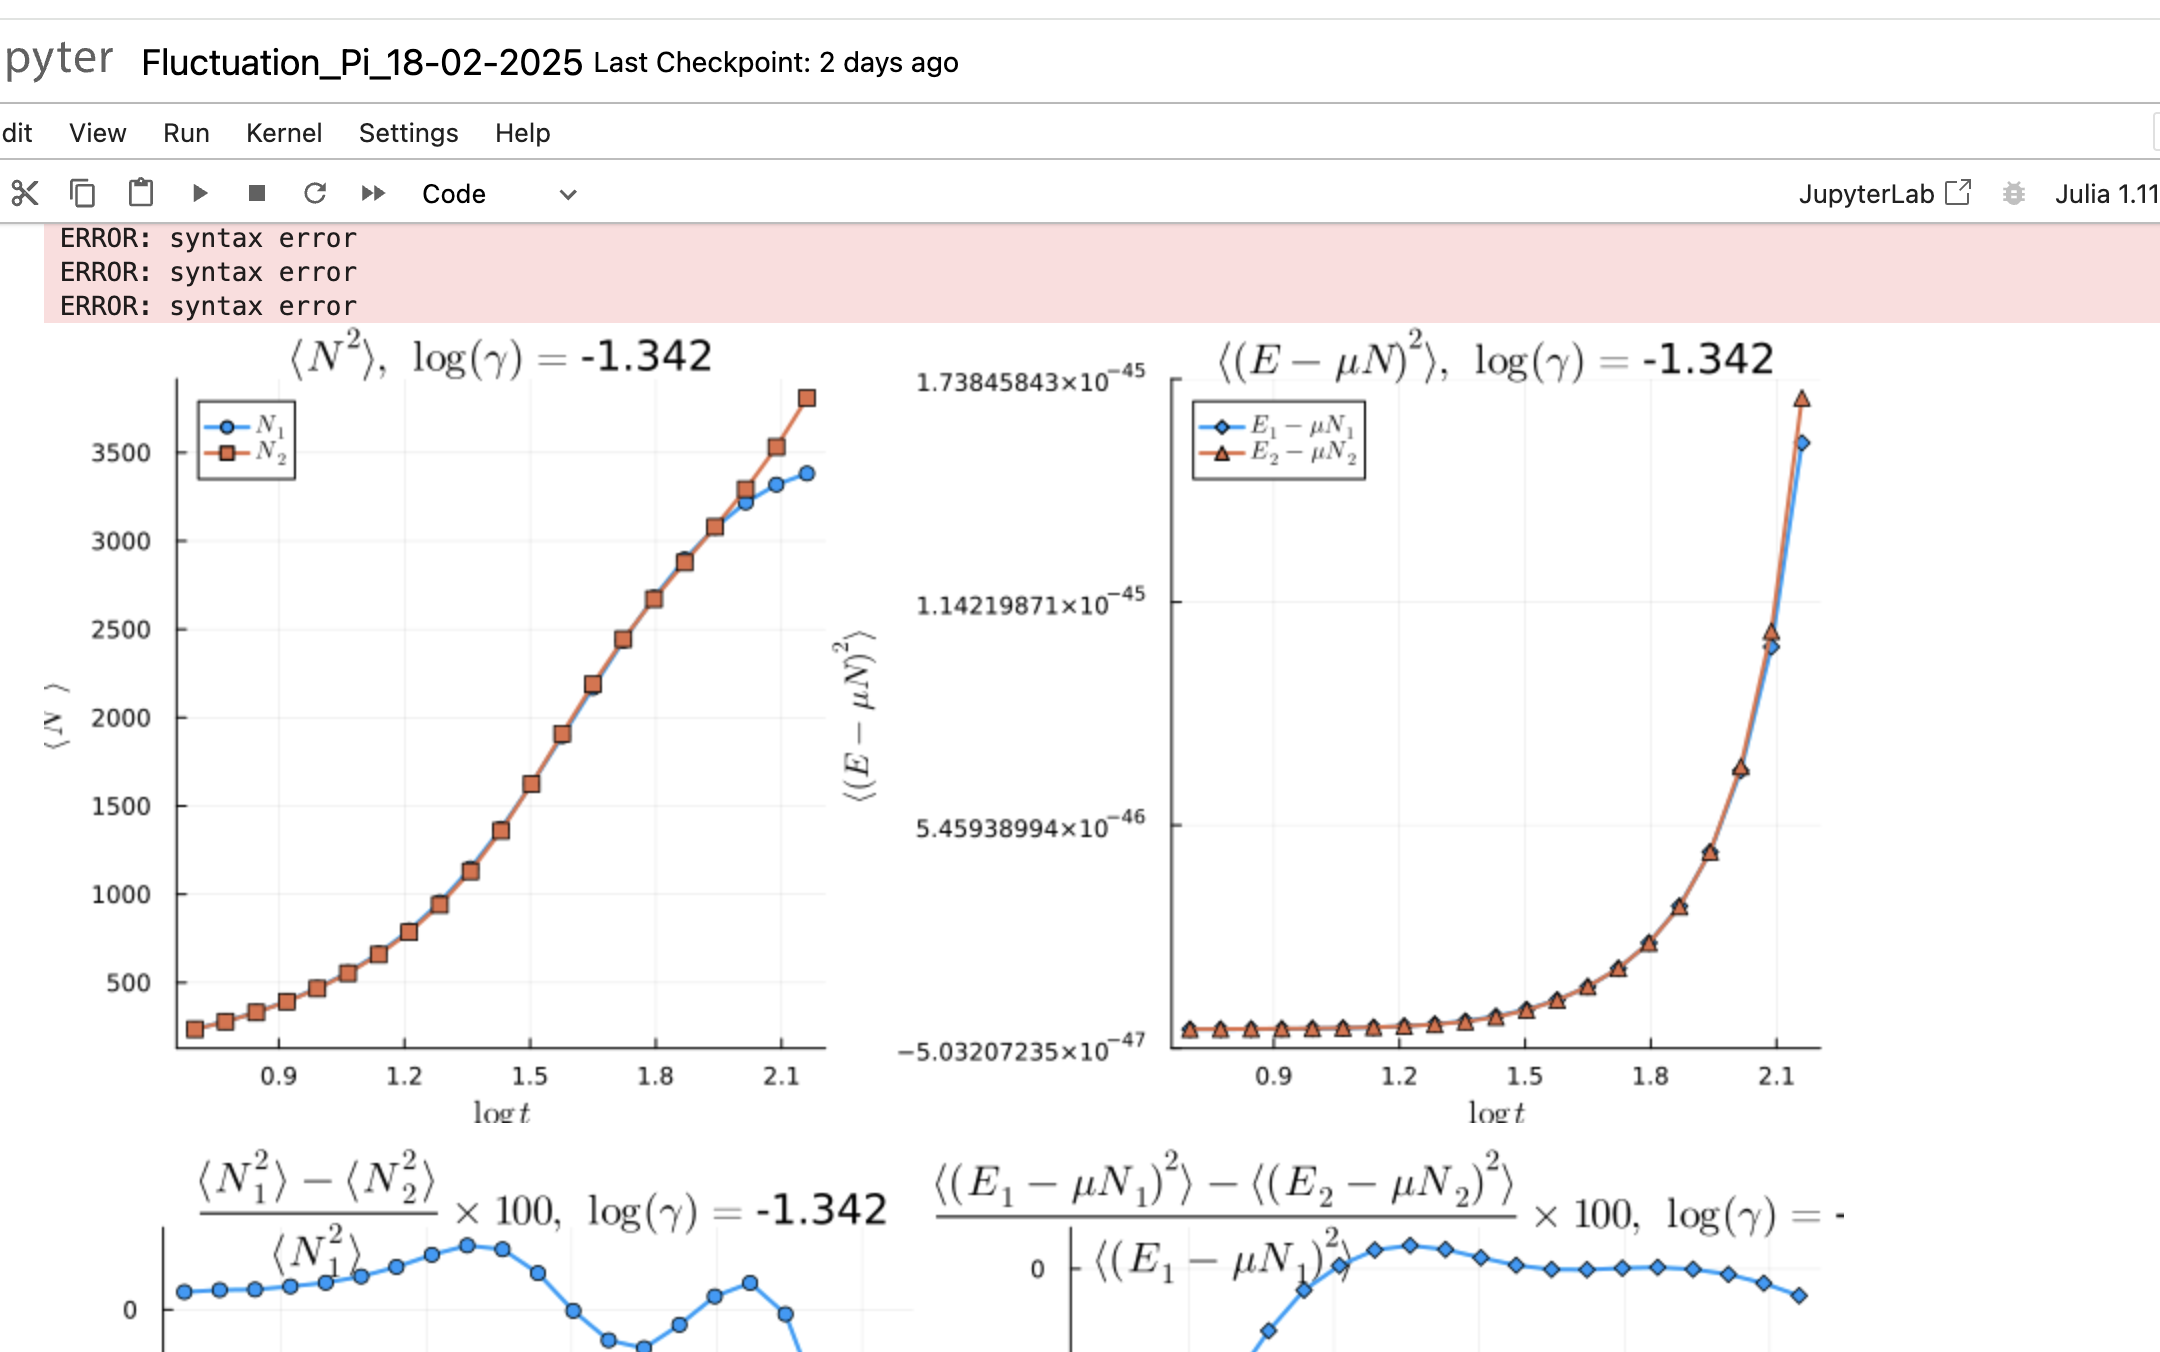
\includegraphics[width=1\textwidth]{Figures/test}

%\begin{aff}
%Donc une a l'ordre un en $\delta \theta (\operator{A}^{(0)})^{-1} %\operator{V}$ 

%\begin{eqnarray*}
%	\langle \delta \Pi ( \theta) \delta \Pi ( \theta') \rangle & = &  ( (\Pi^c_s - \Pi^c)\Pi^c/\Pi^c_s ) ( \theta ) \delta_{\theta, \theta'}/\delta \theta + \mathscr{F}(\theta , \theta' ) ,	
%\end{eqnarray*}

%avec 

%\begin{eqnarray*}
%	\mathscr{F}(\theta , \theta' ) & = & \left [ (\Pi^c_s - \Pi^c )( \theta)  +  (\Pi^c_s - \Pi^c ) ( \theta' )\right ] \frac{\Pi^c}{\Pi^c_s}(\theta)\frac{\Pi^c}{\Pi^c_s}(\theta') \frac{ \Delta( \theta'- \theta )}{ 2 \pi }\\
%	&&  - \left [ (\Pi^c_s - \Pi^c )( \theta)   (\Pi^c_s - \Pi^c ) ( \theta' )\right ] \frac{\Pi^c}{\Pi^c_s}(\theta)\frac{\Pi^c}{\Pi^c_s}(\theta')\int d\theta'' \left (   \frac{ \Pi^c/\Pi^c_s}{\Pi^c_s - \Pi^c} \right )(\theta'') \frac{\Delta(\theta''- \theta)}{2 \pi}\frac{\Delta(\theta''- \theta')}{2 \pi}  	
%\end{eqnarray*}
%\end{aff}



 











\subsection{Lien avec les équations de Bethe}
%Dans ce chapitre, nous nous intéressons aux fluctuations de la distribution de rapidité \( \delta \rho \) autour d'une distribution de référence \( \rho^c \), qui maximise la contribution à la fonction de partition des états, exprimée comme une fonctionnelle de la distribution \( \rho \) : 

La fonction de partition des états, s'exprime comme une fonctionnelle de la distribution \( \rho \) : 

\begin{eqnarray*}
	\Xi & = & \sum_\rho \exp \left( -\mathcal{A}(\rho) \right).
\end{eqnarray*}  

Dans la section {\em \bf Entropie de Yang-Yang} (\ref{??}), l'action \( \mathcal{A}(\rho) \) s'écrit sous la forme :  

\begin{eqnarray*}
	\mathcal{A}(\rho) & \doteq & - L\mathcal{S}_{YY}(\rho) + L\int f(\theta) \rho (\theta) \, d\theta,		
\end{eqnarray*}  

où \( \mathcal{S}_{YY} \) est la fonctionnelle d'entropie de Yang-Yang, définie dans (\ref{??}), et \( f \) est la fonction paramétrant les charges, introduite dans (\ref{??}).  

Dans cette même section {\em \bf Entropie de Yang-Yang} (\ref{??}), nous avons établi un lien entre \( f \) et distribution de référence \( \rho^c \), qui maximise la contribution à la fonction de partition des états .\\

On veux tester si nos experience est décrit pas un GGE. Pour cela nous nous intéressons aux fluctuations de la distribution de rapidité \( \delta \rho \) autour \( \rho^c \).

%Nous poursuivons à présent avec cette définition de l'action de classe $\mathcal{C}^2$ et admetant une distribution critique $\rho^c$ tel que sa différentielle en ce point critique soit nulle $d\mathcal{A}_{\rho^c} = 0 $ (\ref{??}) de sorte que d'aprés la formule de Taylor-Youg %afin de déterminer les fluctuations autour de \( \Pi^c \). Pour cela, nous réécrivons l'action sous la forme :  

Nous poursuivons à présent avec cette définition de l'action de classe $\mathcal{C}^2$ et admetant une distribution critique $\rho^c$ tel que sa différentielle en ce point critique soit nulle $d\mathcal{A}_{\rho^c} = 0 $ (\ref{??}) de sorte que d'aprés la formule de Taylor-Youg %afin de déterminer les fluctuations autour de \( \Pi^c \). Pour cela, nous réécrivons l'action sous la forme :  

\begin{eqnarray*}  
	\mathcal{A}(\rho^c + \delta \rho) & \underset{ \delta \rho \to 0 }{=} & \mathcal{A}(\rho^c)  + \frac{1}{2} \left. \frac{\delta^2 \mathcal{A}}{\delta \rho^2} \right|_{\rho^c} (\delta \rho) + \mathcal{O}((\delta \rho)^3),  
\end{eqnarray*}  

une expression quadratique pour l'action à l'ordre dominant en \( \delta \Pi \) avec $\left. \frac{\delta^2 \mathcal{A}}{\delta \rho^2} \right|_{\rho^c}$ la forme quadratique définie positive (Fig (\ref{fig.fluctu.A})).

\begin{figure}[H]
	\centering 
	\begin{tikzpicture}
		\begin{scope}[shift={(0,0)}]
			\begin{scope}[transform canvas={scale=0.6}]
				\input{Figures/Fonc_A_code}	
			
			\end{scope}
			
			\draw[color = red , scale = 0.5 , draw = none  ] (-2 , -1) rectangle (5, 6) ; 	
		\end{scope}
		
		\begin{scope}[shift={(19,-1)}]
			\begin{scope}[transform canvas={scale=0.6}]
				\input{Figures/Occupation_theta_code}	
			
			\end{scope}
			\begin{scope}[scale=1]
				\draw[color = red , scale = 1 , draw = none  ] (-1 , -1) rectangle (5, 5) ; 
			\end{scope}	
		\end{scope}

		
				
			
	\end{tikzpicture}	
	\captionsetup{skip=10pt} % Ajoute de l’espace après la légende
	\label{fig.fluctu.A}
\end{figure}


On discrétise l'axe des rapidités en  petite cellule de rapidité $[\theta, \theta+\delta\theta]$, qui contient $L\rho(\theta) \delta \theta$ rapidités. 
	



Avec ces petites tranches, la forme quadratique s’écrit :

\begin{eqnarray*}
    \left. \frac{\delta^2 \mathcal{A}}{{\delta \rho}^2} \right|_{\rho^c}(\delta \rho ) &=&  \sum_{a,b \mid \text{tranche}}  
    \delta \rho(\theta_a)  \frac{\partial^2 \mathcal{A}}{\partial \delta \rho(\theta_a) \partial \delta \rho(\theta_b) } (\rho^c)  \delta \rho(\theta_b).
\end{eqnarray*}
Les fluctuations s’écrivent donc :

\begin{eqnarray*}
    \langle \delta \rho ( \theta) \delta \rho ( \theta') \rangle &=&  
    \frac{ \int d\delta \rho \, \delta \rho(\theta) \delta \rho ( \theta') 
    \exp \left( - \frac{1}{2} \sum_{a,b \mid \text{tranche}}  
    \delta \rho(\theta_a) \frac{\partial^2 \mathcal{A}}{\partial \delta \rho(\theta_a) \partial \delta \rho(\theta_b) } (\rho^c)  \delta \rho(\theta_b) \right) }
    { \int d\delta \Pi  
    \exp \left( - \frac{1}{2} \sum_{a,b \mid \text{tranche}}  
    \delta \rho(\theta_a) \frac{\partial^2 \mathcal{A}}{\partial \delta \rho(\theta_a) \partial \delta \rho(\theta_b) } (\rho^c)  \delta \rho(\theta_b) \right) } \\
    &=& \left( \mathbf{A}^{-1} \right)_{\theta , \theta'}
\end{eqnarray*}


\begin{aff}

\begin{eqnarray*}
	\langle \delta \rho ( \theta) \delta \rho ( \theta') \rangle &=& 	\left( \mathbf{A}^{-1} \right)_{\theta , \theta'}
\end{eqnarray*}

	
avec la  {\em matrice hessienne} $\mathbf{A}_{\theta , \theta'} \equiv \frac{\partial^2 \mathcal{A}}{\partial \delta \rho(\theta) \partial \delta \rho(\theta') }(\rho^c)$, au point critique/ qui maximise la probabilité  $\rho^c=\rho^c_s \nu^c $, s'écrit

\begin{eqnarray*}
	\operator{A} & = & \operator{A}^{(0)} + \delta \theta \operator{V}
\end{eqnarray*}

avec 

\begin{eqnarray*}
	A^{(0)}_{\theta , \theta'}  & = &  L\delta \theta \left ( \frac{ 1}{\rho^c_s ( 1  - \nu^c ) \nu^c } \right )(\theta)    \delta({\theta - \theta '})	,\\
	V_{\theta , \theta'}  &= & L \delta \theta \left \{ - \left [ \left ( \frac{1}{\rho^c_s( 1 - \nu^c) } \right ) ( \theta)  +  \left ( \frac{1}{\rho^c_s( 1 - \nu^c) } \right ) ( \theta' )\right ] \frac{ \Delta( \theta'- \theta )}{ 2 \pi } + \int d\theta''  \left ( \frac{\nu^c}{\rho^c_s( 1 - \nu^c) } \right )(\theta'') \frac{\Delta(\theta''- \theta)}{2 \pi}\frac{\Delta(\theta''- \theta')}{2 \pi}   \right \} 	
\end{eqnarray*}

\end{aff}

\subsection{Testes}

\begin{eqnarray*}
	\Delta_{\operator{\mathcal{N}}}^2  & = &  \frac{1}{\beta} \left . \frac{\partial \langle \operator{\mathcal{N}} \rangle}{\partial \mu} \right )_T \\
	\Delta_{\operator{\mathcal{E}}-\mu \operator{\mathcal{N}}}^2  & = &  - \left . \frac{\partial \langle \operator{\mathcal{E}}-\mu \operator{\mathcal{N}} \rangle}{\partial \beta} \right )_\mu 
\end{eqnarray*}

et 

\begin{eqnarray*}
	\Delta_{\operator{\mathcal{N}}}^2  &= & L^2 \int d\theta_a \int d \theta_b \, \langle \delta \rho(\theta_a) \delta \rho(\theta_b) \rangle \\
	\Delta_{\operator{\mathcal{E}}-\mu \operator{\mathcal{N}}}^2  & = & L^2 \int d\theta_a \int d \theta_b \, \left ( - \mu + \frac{1}2 m \theta_a^2  \right  )\left ( - \mu + \frac{1}2 m \theta_b^2  \right  )  \langle \delta \rho(\theta_a) \delta \rho(\theta_b) \rangle
\end{eqnarray*}

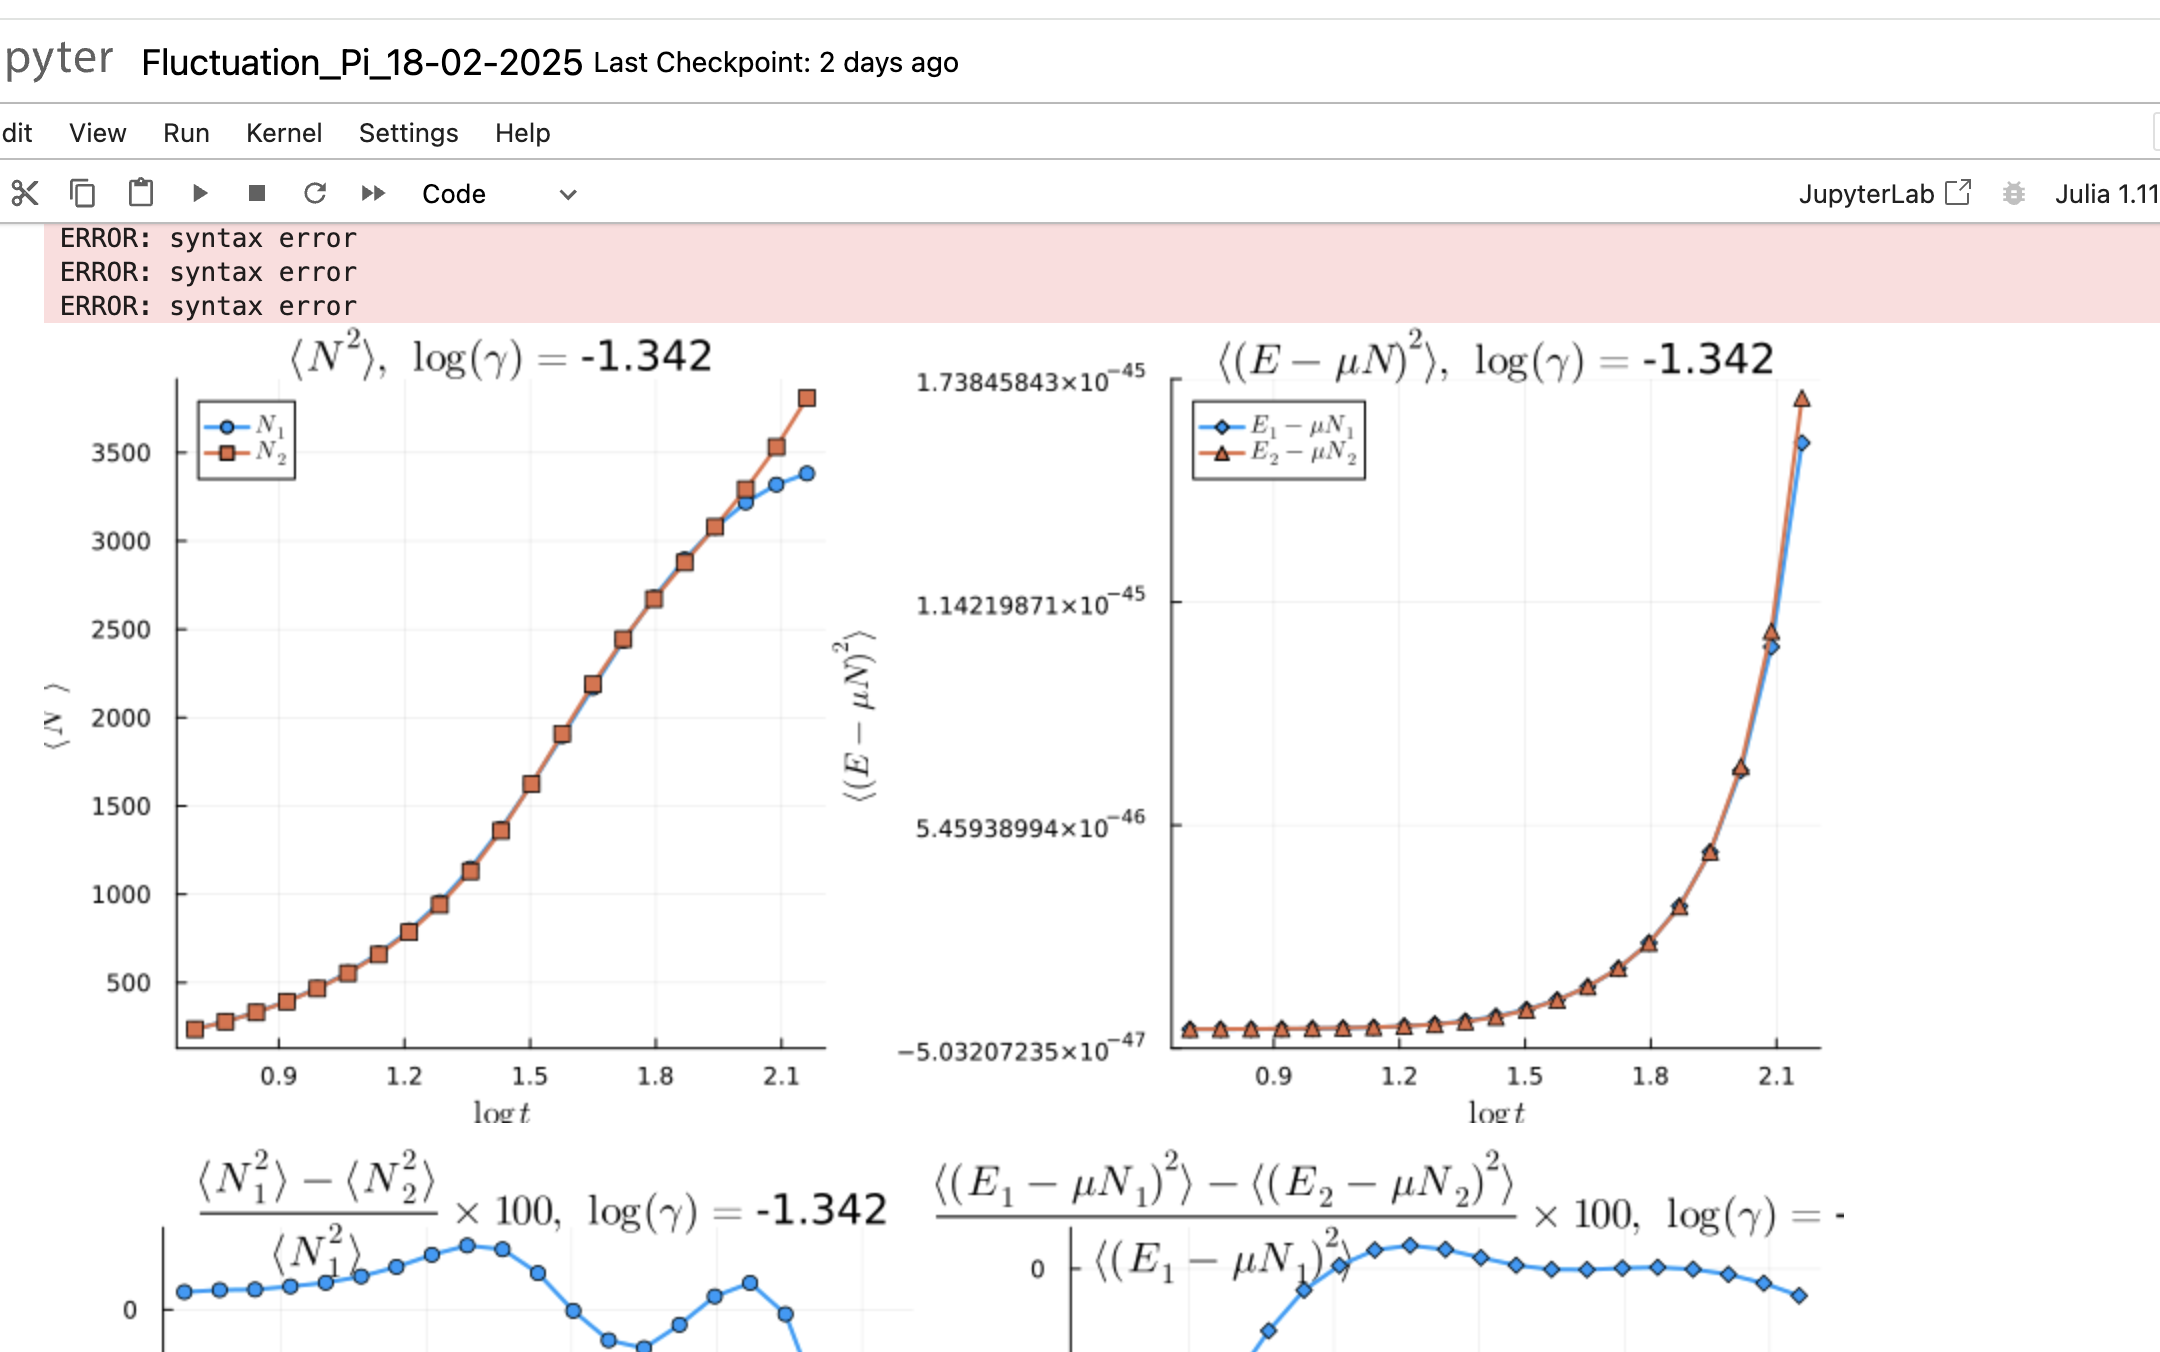
\includegraphics[width=1\textwidth]{Figures/test}

%\begin{aff}
%Donc une a l'ordre un en $\delta \theta (\operator{A}^{(0)})^{-1} %\operator{V}$ 

%\begin{eqnarray*}
%	\langle \delta \Pi ( \theta) \delta \Pi ( \theta') \rangle & = &  ( (\Pi^c_s - \Pi^c)\Pi^c/\Pi^c_s ) ( \theta ) \delta_{\theta, \theta'}/\delta \theta + \mathscr{F}(\theta , \theta' ) ,	
%\end{eqnarray*}

%avec 

%\begin{eqnarray*}
%	\mathscr{F}(\theta , \theta' ) & = & \left [ (\Pi^c_s - \Pi^c )( \theta)  +  (\Pi^c_s - \Pi^c ) ( \theta' )\right ] \frac{\Pi^c}{\Pi^c_s}(\theta)\frac{\Pi^c}{\Pi^c_s}(\theta') \frac{ \Delta( \theta'- \theta )}{ 2 \pi }\\
%	&&  - \left [ (\Pi^c_s - \Pi^c )( \theta)   (\Pi^c_s - \Pi^c ) ( \theta' )\right ] \frac{\Pi^c}{\Pi^c_s}(\theta)\frac{\Pi^c}{\Pi^c_s}(\theta')\int d\theta'' \left (   \frac{ \Pi^c/\Pi^c_s}{\Pi^c_s - \Pi^c} \right )(\theta'') \frac{\Delta(\theta''- \theta)}{2 \pi}\frac{\Delta(\theta''- \theta')}{2 \pi}  	
%\end{eqnarray*}
%\end{aff}



 



















%\subsection{Vérification explicite de la condition aux limites}
%%Dans ce chapitre, nous nous intéressons aux fluctuations de la distribution de rapidité \( \delta \rho \) autour d'une distribution de référence \( \rho^c \), qui maximise la contribution à la fonction de partition des états, exprimée comme une fonctionnelle de la distribution \( \rho \) : 

La fonction de partition des états, s'exprime comme une fonctionnelle de la distribution \( \rho \) : 

\begin{eqnarray*}
	\Xi & = & \sum_\rho \exp \left( -\mathcal{A}(\rho) \right).
\end{eqnarray*}  

Dans la section {\em \bf Entropie de Yang-Yang} (\ref{??}), l'action \( \mathcal{A}(\rho) \) s'écrit sous la forme :  

\begin{eqnarray*}
	\mathcal{A}(\rho) & \doteq & - L\mathcal{S}_{YY}(\rho) + L\int f(\theta) \rho (\theta) \, d\theta,		
\end{eqnarray*}  

où \( \mathcal{S}_{YY} \) est la fonctionnelle d'entropie de Yang-Yang, définie dans (\ref{??}), et \( f \) est la fonction paramétrant les charges, introduite dans (\ref{??}).  

Dans cette même section {\em \bf Entropie de Yang-Yang} (\ref{??}), nous avons établi un lien entre \( f \) et distribution de référence \( \rho^c \), qui maximise la contribution à la fonction de partition des états .\\

On veux tester si nos experience est décrit pas un GGE. Pour cela nous nous intéressons aux fluctuations de la distribution de rapidité \( \delta \rho \) autour \( \rho^c \).

%Nous poursuivons à présent avec cette définition de l'action de classe $\mathcal{C}^2$ et admetant une distribution critique $\rho^c$ tel que sa différentielle en ce point critique soit nulle $d\mathcal{A}_{\rho^c} = 0 $ (\ref{??}) de sorte que d'aprés la formule de Taylor-Youg %afin de déterminer les fluctuations autour de \( \Pi^c \). Pour cela, nous réécrivons l'action sous la forme :  

Nous poursuivons à présent avec cette définition de l'action de classe $\mathcal{C}^2$ et admetant une distribution critique $\rho^c$ tel que sa différentielle en ce point critique soit nulle $d\mathcal{A}_{\rho^c} = 0 $ (\ref{??}) de sorte que d'aprés la formule de Taylor-Youg %afin de déterminer les fluctuations autour de \( \Pi^c \). Pour cela, nous réécrivons l'action sous la forme :  

\begin{eqnarray*}  
	\mathcal{A}(\rho^c + \delta \rho) & \underset{ \delta \rho \to 0 }{=} & \mathcal{A}(\rho^c)  + \frac{1}{2} \left. \frac{\delta^2 \mathcal{A}}{\delta \rho^2} \right|_{\rho^c} (\delta \rho) + \mathcal{O}((\delta \rho)^3),  
\end{eqnarray*}  

une expression quadratique pour l'action à l'ordre dominant en \( \delta \Pi \) avec $\left. \frac{\delta^2 \mathcal{A}}{\delta \rho^2} \right|_{\rho^c}$ la forme quadratique définie positive (Fig (\ref{fig.fluctu.A})).

\begin{figure}[H]
	\centering 
	\begin{tikzpicture}
		\begin{scope}[shift={(0,0)}]
			\begin{scope}[transform canvas={scale=0.6}]
				% Définition des couleurs avec les codes HTML
\definecolor{colorOne}{HTML}{443E46}
\definecolor{colorTwo}{HTML}{F6DEB8}
\definecolor{colorThree}{HTML}{908CA4}
\definecolor{colorFour}{HTML}{57659E}
\definecolor{colorFive}{HTML}{C57284}
\definecolor{colorSix}{HTML}{FF5B69}

% Raccourcis pour les couleurs
\def\colorOne{colorOne}
\def\colorTwo{colorTwo}
\def\colorThree{colorThree}
\def\colorFour{colorFour}
\def\colorFive{colorFive}
\def\colorSix{colorSix}

\def\colorslide{blue!50!black}



\begin{scope}
	% Tracer une courbe lisse entre des points
	\draw[shift={(0,0)} ,\colorOne]
		(-1 , 0 ) edge [thick,line width=0.8ex , ->,>=triangle 45  , \colorOne] node [pos = 1 , below ]{\huge$\rho$}( 5  , 0 )
	;
	\draw[shift={(0,0)}, color=\colorOne]
		(0, -1.0 ) edge [thick,line width=0.8ex , ->,>=triangle 45  ]node [pos=0.9,left=0.2cm ]{\huge$\mathcal{A}(\rho)$}( 0  , 5 )
	;
	\draw[]
		(2.5, 0.12 ) edge [thick,line width=0.8ex ,\colorThree ]node [pos=1,below  ]{\huge$\rho^c$} (2.5, -0.12 )	
	;
	
	\draw[]
		(2.5, -0.12 ) edge [thick,line width=0.4ex , dashed, \colorThree ] (2.5, 5.5 )
		(1.5, 1 ) edge [thick,line width=0.4ex , <->,>=triangle 45  , \colorThree ] (3.5, 1 )
		(-0.3,1) edge [thick,line width=0.4ex  , \colorThree ] node [pos=0,left ]{\huge$\mathcal{A}(\rho^c)$} (0.3, 1 )	
	;
    \draw[thick, line width=0.8ex , \colorFour] plot[smooth, tension=0.7] coordinates {
        (1, 5) (1.6 , 3 ) (2.5, 1) (3.5 , 3 )  (4, 5)
    };		
	
\end{scope}

	
			
			\end{scope}
			
			\draw[color = red , scale = 0.5 , draw = none  ] (-2 , -1) rectangle (5, 6) ; 	
		\end{scope}
		
		\begin{scope}[shift={(19,-1)}]
			\begin{scope}[transform canvas={scale=0.6}]
				% Définition des couleurs avec les codes HTML
\definecolor{colorOne}{HTML}{443E46}
\definecolor{colorTwo}{HTML}{F6DEB8}
\definecolor{colorThree}{HTML}{908CA4}
\definecolor{colorFour}{HTML}{57659E}
\definecolor{colorFive}{HTML}{C57284}
\definecolor{colorSix}{HTML}{FF5B69}

% Raccourcis pour les couleurs
\def\colorOne{colorOne}
\def\colorTwo{colorTwo}
\def\colorThree{colorThree}
\def\colorFour{colorFour}
\def\colorFive{colorFive}
\def\colorSix{colorSix}

\def\colorslide{blue!50!black}

\def\Occupation{
	\def\traitx{0.3}
	\def\traity{0.5}
	\draw[shift={(0,0)}]
		(-13.5 , 0 ) edge [thick,line width=0.8ex ]( -3.2  , 0 )
		( -3.2 - \traitx  , 0 - \traity ) edge [thick,line width=0.8ex ]( -3.2 + \traitx  , 0 + \traity  )
		( -2.8 - \traitx  , 0 - \traity ) edge [thick,line width=0.8ex ]( -2.8 + \traitx  , 0 + \traity  )
		(-2.8 , 0 ) edge [thick,line width=0.8ex ](2.8  , 0 )
		( 2.8 - \traitx  , 0 - \traity ) edge [thick,line width=0.8ex ]( 2.8 + \traitx  , 0 + \traity  )
		( 3.2 - \traitx  , 0 - \traity ) edge [thick,line width=0.8ex ]( 3.2 + \traitx  , 0 + \traity  )
		(3.2, 0 ) edge [thick,line width=0.8ex,->,>=triangle 45 , color = black ]node [pos=1.01,below  ]{\huge$\theta$}	( 13  , 0 )
	;
	\draw[shift={(0,0)}, color=\colorOne]
		(-10.5 , -1.5 ) edge [thick,line width=0.8ex , ->,>=triangle 45  ]( -10.5  , 4.5 )
	;
		
	\foreach \r in {1 , ... , 3 } {
%		\draw[
%		decoration={
%		markings,
%    	mark connection node=my node,
%    	mark=at position 0 with{\node [blue,transform shape] (my node) {\large \r};}},
%		color=gray, thick, 
%		line width=0.5ex] decorate { 
%            (-11.0, \r) -- (-10.1, \r )}
%        ;
        \draw[
			color=\colorOne,
			] 
            (-11.0, \r) edge[color=\colorThree , thick,line width=0.5ex] node [pos=-0.5 ]{\large\color{\colorFour} $\frac{\r}{\delta \theta}$ } (-10.3, \r )
        	;
	
	}
	

	
	% Graduation abcsisse 
	% Définitions des listes
% Definitions of the lists
\def\listetuple{-9/\theta_{1}, -8/\theta_{2} , -5/\theta_{3} , -2/\theta_{a-1} , 0/\theta_{a} , 1/\theta_{a+1} , 2/\theta_{a+2} ,  5/\theta_{N-4} , 7/\theta_{N-3},8/\theta_{N-1},9/\theta_{N} }
\def\listetrais{-12 , -11, -10, -9 , -8 , -7 ,  -6 , -5, -4.5,-4, -2 , -1, 0 , 0.5, 1, 2, 4 , 5 ,  6 , 7 , 8 ,8.5, 9 ,  10 , 11, 12 }

% Loop over listetrais
\foreach \r in \listetrais {
    % Initialize found variable to zero
    % Initialize found variable to zero
    %\pgfmathsetmacro\found{0}
    \global\def\found{0}
    \xdef\nomtheta{}
    
    % Check if \r is in listetuple
    \foreach \x/\y in \listetuple { 
        \ifdim \r pt=\x pt % If \r matches any \x in listetuple
            \global\def\found{1} ;
            \xdef\nomtheta{\y} % Set \nomtheta to the corresponding \y
            %\pgfmathsetmacro\found{1} % Set found to 1            
            %\global\pgfmathsetmacro\found{1}
        \fi
    }
    
    %\node [circle, draw, red] (A) at (\r, 2) {\found , $\nomtheta$};
    
    % Draw the line and display \nomtheta if found
    \ifnum\found=1
        \draw[color=\colorOne, thick, line width=0.5ex] 
            (\r, -0.3) -- (\r, 0.3) node[red , pos=-0.5] {\large $\nomtheta$};
         \filldraw[line width=0.5ex, color=\colorSix, outer color=\colorSix, inner color=\colorSix] 
            (\r, 0) circle (4pt);
    \else 
        % Draw without \nomtheta and add a blue circle if not found
        \draw[color=\colorOne, thick, line width=0.5ex] 
            (\r, -0.3) -- (\r, 0.3);
        \filldraw[line width=0.5ex, color=\colorSix, outer color=\colorTwo, inner color=\colorTwo] 
            (\r, 0) circle (4pt); 
    \fi
}

\def\listetrais{-9.5/\theta_{i-1}/2/3, -6.5/\theta_{i}/1/4  ,   -1.5/\theta_{j}/2/4 , 1.5/\theta_{j+1}/-1/3 , 3.5/\theta_{\ell-1}/1/3 , 6.5/\theta_{\ell}/3/4 , 9.5/\theta(\theta_{\ell+1})/-1/3 };



\foreach \r/\nomx/\y/\ys in \listetrais {
	\draw[
		decoration={
		markings,
    	mark connection node=my node,
    	mark=at position .5 with{\node [blue,transform shape] (my node) {\large \color{\colorFour} $\nomx$};}},
		color=\colorThree , thick, 
		line width=0.5ex] decorate { 
            (\r, 0.12) -- (\r, -1.2)}
        ;
     
     \ifdim \y pt > -1 pt 
     	\draw[
			decoration={
			markings,
    		mark connection node=my node,
    		mark=at position .5 with{\node [blue,transform shape] (my node) {\large \color{\colorFour} $\Pi(\nomx) $};}},
			color=\colorThree, thick, 
			line width=0.5ex] decorate { 
            (\r, \y) -- (\r +3, \y)}
        ;
        \draw[
			decoration={
			markings,
    		mark connection node=my node,
    		mark=at position .5 with{\node [blue,transform shape] (my node) {\large \color{\colorFive} $\Pi_s(\nomx) $};}},
			color=\colorFive, thick, 
			line width=0.5ex] decorate { 
            (\r, \ys) -- (\r +3, \ys)}
        ;
     \fi 
     \ifdim \r pt= -1.5 pt
     	\draw[
     		decoration={
			markings,
    		mark connection node=my node,
    		mark=at position .5 with{\node [blue,transform shape] (my node) {\large \color{\colorFour}  $\delta \theta $};},
    		%mark=at position 0.1  with {\arrow[blue, line width=0.5ex]{<}},
    		%mark=at position 1  with {\arrow[blue, line width=0.5ex]{>}}
    		},
        	color=\colorThree,
        	thick,
        	line width=0.5ex,
        	%arrows={Computer Modern Rightarrow[line cap=round]-Computer Modern Rightarrow[line cap=round]}
   			](\r, -1.2) edge[arrows={Computer Modern Rightarrow[line cap=round]-}] (\r + 0.4, -1.2)decorate {
    		(\r, -1.2) -- (\r + 3, -1.2)}(\r + 2, -1.2) edge[arrows={-Computer Modern Rightarrow[line cap=round]}] (\r + 3, -1.2)
    		;
    \fi
			
	
}


			
}


\begin{scope}
	%\draw[help lines , width=1.5ex] (-8,-3) grid (8,3);\draw[help lines ,width=0.5ex , opacity = 0.5] (-3,-3) grid[step=0.1] (3,3));
	
	%\draw[help lines] 
	%	(-3,-3) edge[width=1.5ex] grid (3,3)	
	%	(-3,-3) edge[width=0.5ex , opacity = 0.5] grid (3,3)	
	%;
	\begin{scope}[shift={(0,1)},rotate=0,opacity=1,color=black]
		\Occupation	
		
		%\node[anchor=east, font=\bfseries] at (-11, 0) {\color{red}\large (T = 0 )} ;	
	\end{scope}
	
	
	
	
	\begin{scope}[shift={(-10.5,7)},rotate=0,opacity=1,color=black]
	
	\begin{scope}[shift={(-0,0)},rotate=0,opacity=1,color=black]
	
		\draw[shift={(0,0)} ,line width=1ex,rounded corners = 1ex,color=\colorOne , opacity =1 ,fill=\colorOne!00 , pattern={north east lines} , pattern color=\colorOne!00 ]
			(0 , -1 ) rectangle (5,1)
		;
		

		\begin{scope}[shift={(0.5,0.5)}]
			\draw[color=\colorOne, thick, line width=0.5ex] 
            (0, -0.3) -- (0, 0.3) ;
            \filldraw[line width=0.5ex, color=\colorSix, outer color=\colorSix, inner color=\colorSix] 
            (0, 0) circle (4pt);
            
            \node[anchor=west, font=\bfseries] at (0.2, 0) {\color{\colorSix}\large : quasi-particule};
		\end{scope}
		
		\begin{scope}[shift={(0.5,-0.5)}]
			\draw[color=\colorOne, thick, line width=0.5ex] 
            (0, -0.3) -- (0, 0.3) ;
            \filldraw[line width=0.5ex, color=\colorSix, outer color=\colorTwo, inner color=\colorTwo] 
            (0, 0) circle (4pt);
            
            \node[anchor=west, font=\bfseries] at (0.2, 0) {\color{\colorSix}\large : hole};
		\end{scope}

	\end{scope}
	
	\begin{scope}[shift={(6,0)},rotate=0,opacity=1,color=black]	
		
		\draw[shift={(0,0)} ,line width=1ex,rounded corners = 1ex,color=\colorOne , opacity =1 ,fill=\colorOne!00 , pattern={north east lines} , pattern color=\colorOne!00 ]
			(0 , -1 ) rectangle (7.5,1)
		;
		
		\node[anchor=west] at (0.5, 0.5) {\color{\colorFour}\large $\Pi$ };\node[anchor=west, font=\bfseries] at (1, 0.5) {\color{\colorFour}\large : quasi-particule distribution};
		
		\node[anchor=west] at (0.5, -0.5) {\color{\colorFour}\large $\Pi_h$ };\node[anchor=west, font=\bfseries] at (1, -0.5) {\color{\colorFour}\large  : hole distribution};
		
	\end{scope}
	
	\begin{scope}[shift={(14.5,0)},rotate=0,opacity=1,color=black]	
		
		\draw[shift={(0,0)} ,line width=1ex,rounded corners = 1ex,color=\colorOne , opacity =1 ,fill=\colorOne!00 , pattern={north east lines} , pattern color=\colorOne!00 ]
			(0 , -0.5 ) rectangle (7.0,0.5)
		;
		
		\node[anchor=west] at (0.2, 0) {\color{\colorFour}\large ${\color{\colorFive}\Pi_s} = \Pi + \Pi_h $ } node[anchor=west , font=\bfseries] at (3.1 , 0 )  {\color{\colorFour}\large {\color{\colorFive} : density of states}};
		
	\end{scope}
	
	
	\end{scope}


		
	
\end{scope}

	
			
			\end{scope}
			\begin{scope}[scale=1]
				\draw[color = red , scale = 1 , draw = none  ] (-1 , -1) rectangle (5, 5) ; 
			\end{scope}	
		\end{scope}

		
				
			
	\end{tikzpicture}	
	\captionsetup{skip=10pt} % Ajoute de l’espace après la légende
	\label{fig.fluctu.A}
\end{figure}


On discrétise l'axe des rapidités en  petite cellule de rapidité $[\theta, \theta+\delta\theta]$, qui contient $L\rho(\theta) \delta \theta$ rapidités. 
	



Avec ces petites tranches, la forme quadratique s’écrit :

\begin{eqnarray*}
    \left. \frac{\delta^2 \mathcal{A}}{{\delta \rho}^2} \right|_{\rho^c}(\delta \rho ) &=&  \sum_{a,b \mid \text{tranche}}  
    \delta \rho(\theta_a)  \frac{\partial^2 \mathcal{A}}{\partial \delta \rho(\theta_a) \partial \delta \rho(\theta_b) } (\rho^c)  \delta \rho(\theta_b).
\end{eqnarray*}
Les fluctuations s’écrivent donc :

\begin{eqnarray*}
    \langle \delta \rho ( \theta) \delta \rho ( \theta') \rangle &=&  
    \frac{ \int d\delta \rho \, \delta \rho(\theta) \delta \rho ( \theta') 
    \exp \left( - \frac{1}{2} \sum_{a,b \mid \text{tranche}}  
    \delta \rho(\theta_a) \frac{\partial^2 \mathcal{A}}{\partial \delta \rho(\theta_a) \partial \delta \rho(\theta_b) } (\rho^c)  \delta \rho(\theta_b) \right) }
    { \int d\delta \Pi  
    \exp \left( - \frac{1}{2} \sum_{a,b \mid \text{tranche}}  
    \delta \rho(\theta_a) \frac{\partial^2 \mathcal{A}}{\partial \delta \rho(\theta_a) \partial \delta \rho(\theta_b) } (\rho^c)  \delta \rho(\theta_b) \right) } \\
    &=& \left( \mathbf{A}^{-1} \right)_{\theta , \theta'}
\end{eqnarray*}


\begin{aff}

\begin{eqnarray*}
	\langle \delta \rho ( \theta) \delta \rho ( \theta') \rangle &=& 	\left( \mathbf{A}^{-1} \right)_{\theta , \theta'}
\end{eqnarray*}

	
avec la  {\em matrice hessienne} $\mathbf{A}_{\theta , \theta'} \equiv \frac{\partial^2 \mathcal{A}}{\partial \delta \rho(\theta) \partial \delta \rho(\theta') }(\rho^c)$, au point critique/ qui maximise la probabilité  $\rho^c=\rho^c_s \nu^c $, s'écrit

\begin{eqnarray*}
	\operator{A} & = & \operator{A}^{(0)} + \delta \theta \operator{V}
\end{eqnarray*}

avec 

\begin{eqnarray*}
	A^{(0)}_{\theta , \theta'}  & = &  L\delta \theta \left ( \frac{ 1}{\rho^c_s ( 1  - \nu^c ) \nu^c } \right )(\theta)    \delta({\theta - \theta '})	,\\
	V_{\theta , \theta'}  &= & L \delta \theta \left \{ - \left [ \left ( \frac{1}{\rho^c_s( 1 - \nu^c) } \right ) ( \theta)  +  \left ( \frac{1}{\rho^c_s( 1 - \nu^c) } \right ) ( \theta' )\right ] \frac{ \Delta( \theta'- \theta )}{ 2 \pi } + \int d\theta''  \left ( \frac{\nu^c}{\rho^c_s( 1 - \nu^c) } \right )(\theta'') \frac{\Delta(\theta''- \theta)}{2 \pi}\frac{\Delta(\theta''- \theta')}{2 \pi}   \right \} 	
\end{eqnarray*}

\end{aff}

\subsection{Testes}

\begin{eqnarray*}
	\Delta_{\operator{\mathcal{N}}}^2  & = &  \frac{1}{\beta} \left . \frac{\partial \langle \operator{\mathcal{N}} \rangle}{\partial \mu} \right )_T \\
	\Delta_{\operator{\mathcal{E}}-\mu \operator{\mathcal{N}}}^2  & = &  - \left . \frac{\partial \langle \operator{\mathcal{E}}-\mu \operator{\mathcal{N}} \rangle}{\partial \beta} \right )_\mu 
\end{eqnarray*}

et 

\begin{eqnarray*}
	\Delta_{\operator{\mathcal{N}}}^2  &= & L^2 \int d\theta_a \int d \theta_b \, \langle \delta \rho(\theta_a) \delta \rho(\theta_b) \rangle \\
	\Delta_{\operator{\mathcal{E}}-\mu \operator{\mathcal{N}}}^2  & = & L^2 \int d\theta_a \int d \theta_b \, \left ( - \mu + \frac{1}2 m \theta_a^2  \right  )\left ( - \mu + \frac{1}2 m \theta_b^2  \right  )  \langle \delta \rho(\theta_a) \delta \rho(\theta_b) \rangle
\end{eqnarray*}

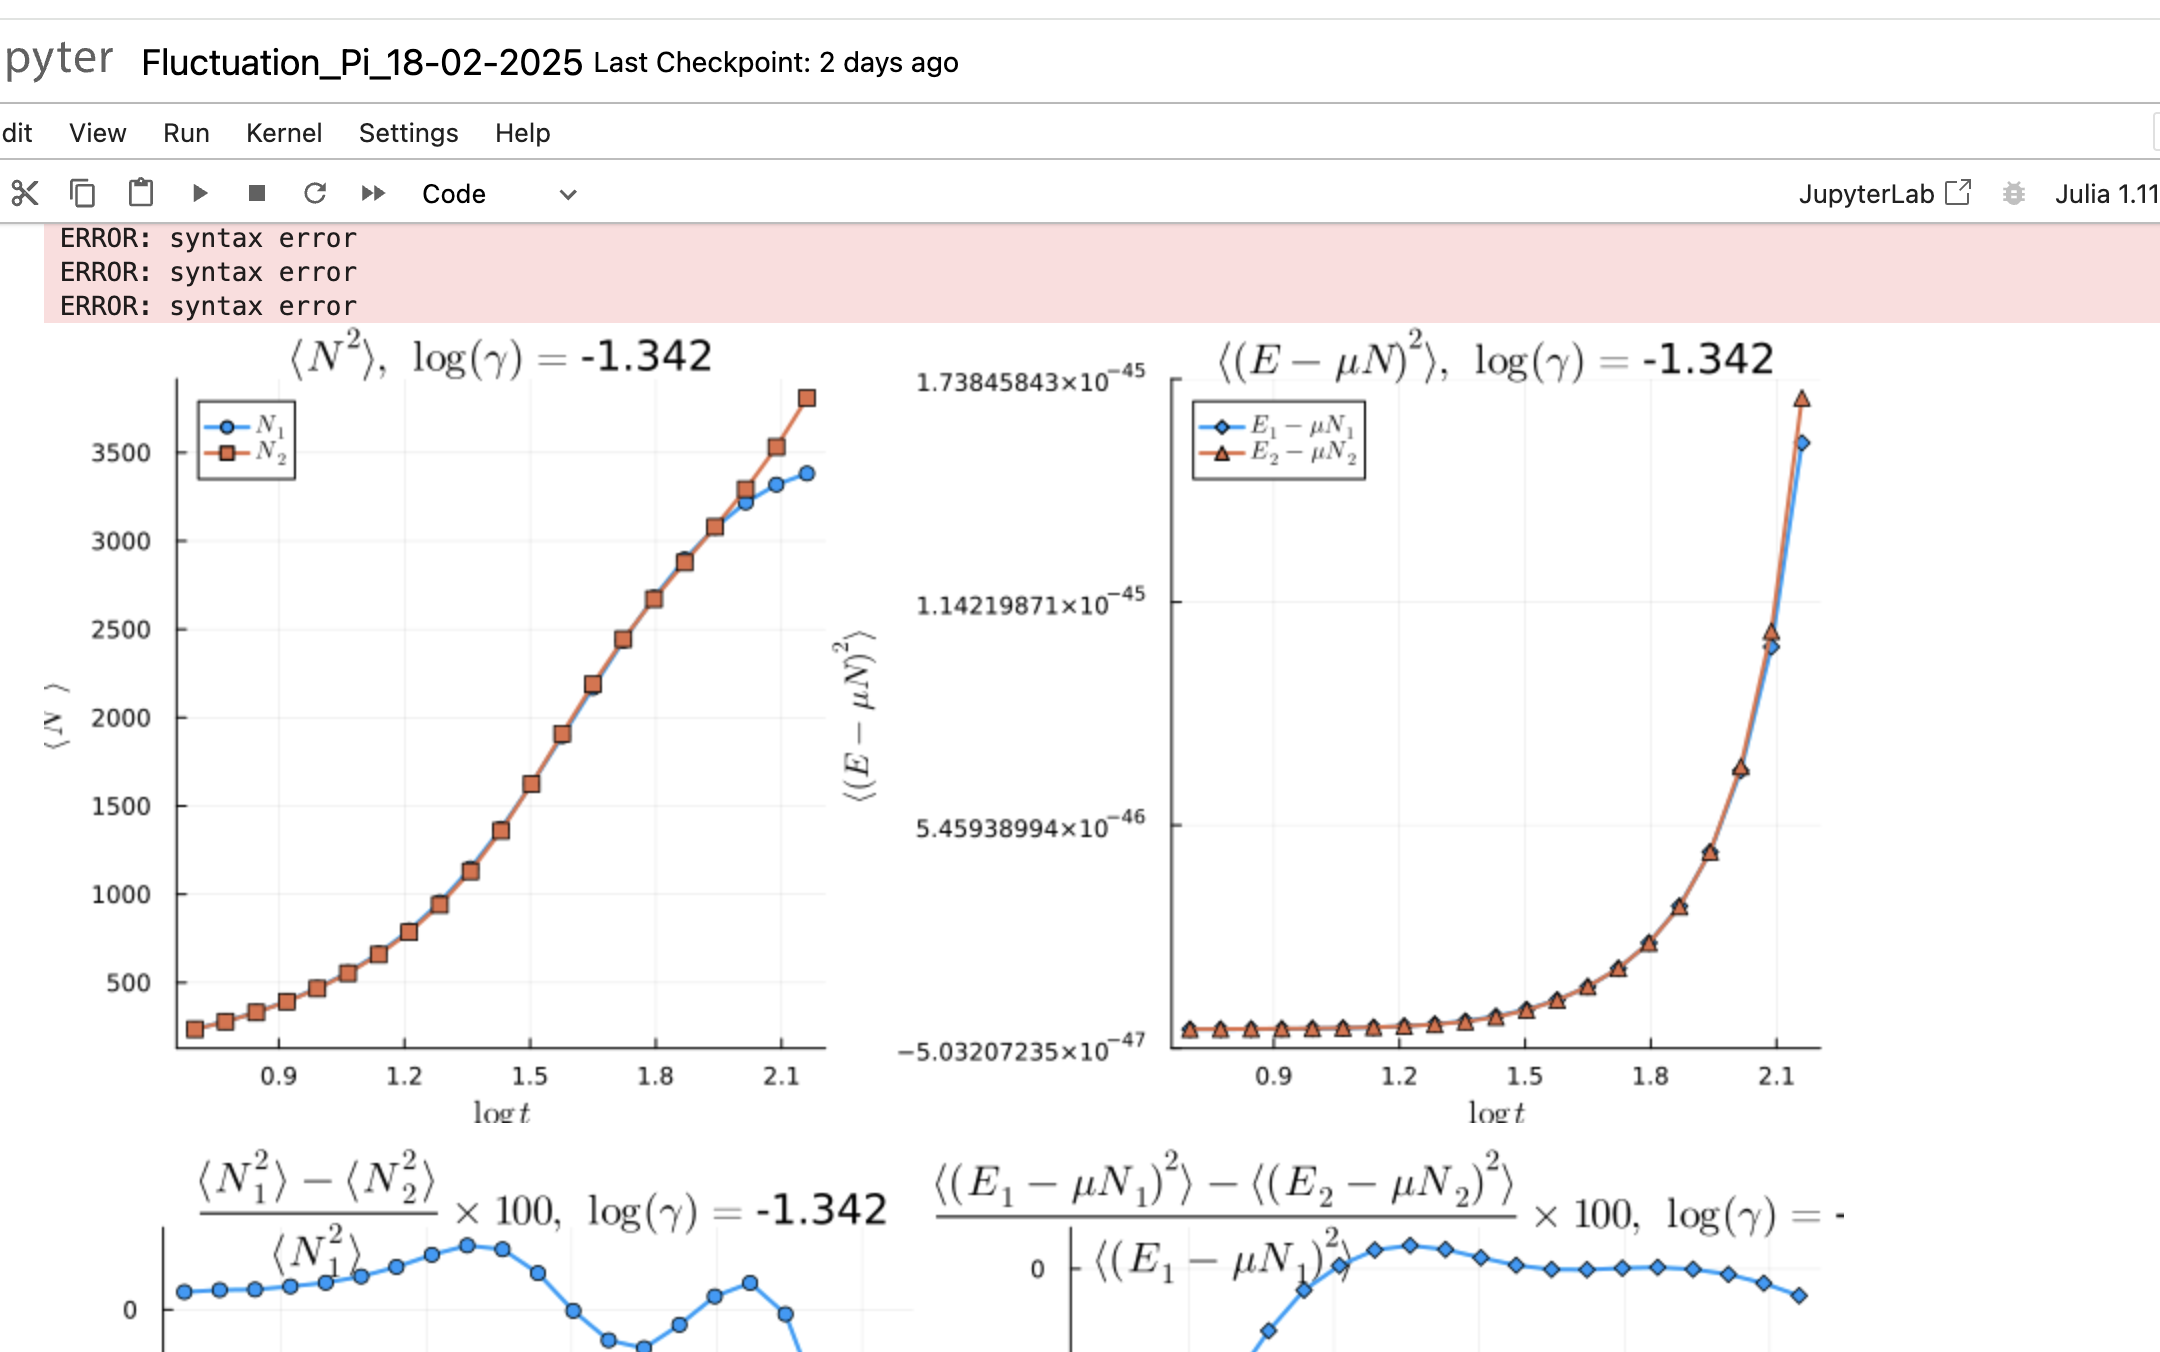
\includegraphics[width=1\textwidth]{Figures/test}

%\begin{aff}
%Donc une a l'ordre un en $\delta \theta (\operator{A}^{(0)})^{-1} %\operator{V}$ 

%\begin{eqnarray*}
%	\langle \delta \Pi ( \theta) \delta \Pi ( \theta') \rangle & = &  ( (\Pi^c_s - \Pi^c)\Pi^c/\Pi^c_s ) ( \theta ) \delta_{\theta, \theta'}/\delta \theta + \mathscr{F}(\theta , \theta' ) ,	
%\end{eqnarray*}

%avec 

%\begin{eqnarray*}
%	\mathscr{F}(\theta , \theta' ) & = & \left [ (\Pi^c_s - \Pi^c )( \theta)  +  (\Pi^c_s - \Pi^c ) ( \theta' )\right ] \frac{\Pi^c}{\Pi^c_s}(\theta)\frac{\Pi^c}{\Pi^c_s}(\theta') \frac{ \Delta( \theta'- \theta )}{ 2 \pi }\\
%	&&  - \left [ (\Pi^c_s - \Pi^c )( \theta)   (\Pi^c_s - \Pi^c ) ( \theta' )\right ] \frac{\Pi^c}{\Pi^c_s}(\theta)\frac{\Pi^c}{\Pi^c_s}(\theta')\int d\theta'' \left (   \frac{ \Pi^c/\Pi^c_s}{\Pi^c_s - \Pi^c} \right )(\theta'') \frac{\Delta(\theta''- \theta)}{2 \pi}\frac{\Delta(\theta''- \theta')}{2 \pi}  	
%\end{eqnarray*}
%\end{aff}



 











%\subsection{Lien avec les équations de Bethe}
%%Dans ce chapitre, nous nous intéressons aux fluctuations de la distribution de rapidité \( \delta \rho \) autour d'une distribution de référence \( \rho^c \), qui maximise la contribution à la fonction de partition des états, exprimée comme une fonctionnelle de la distribution \( \rho \) : 

La fonction de partition des états, s'exprime comme une fonctionnelle de la distribution \( \rho \) : 

\begin{eqnarray*}
	\Xi & = & \sum_\rho \exp \left( -\mathcal{A}(\rho) \right).
\end{eqnarray*}  

Dans la section {\em \bf Entropie de Yang-Yang} (\ref{??}), l'action \( \mathcal{A}(\rho) \) s'écrit sous la forme :  

\begin{eqnarray*}
	\mathcal{A}(\rho) & \doteq & - L\mathcal{S}_{YY}(\rho) + L\int f(\theta) \rho (\theta) \, d\theta,		
\end{eqnarray*}  

où \( \mathcal{S}_{YY} \) est la fonctionnelle d'entropie de Yang-Yang, définie dans (\ref{??}), et \( f \) est la fonction paramétrant les charges, introduite dans (\ref{??}).  

Dans cette même section {\em \bf Entropie de Yang-Yang} (\ref{??}), nous avons établi un lien entre \( f \) et distribution de référence \( \rho^c \), qui maximise la contribution à la fonction de partition des états .\\

On veux tester si nos experience est décrit pas un GGE. Pour cela nous nous intéressons aux fluctuations de la distribution de rapidité \( \delta \rho \) autour \( \rho^c \).

%Nous poursuivons à présent avec cette définition de l'action de classe $\mathcal{C}^2$ et admetant une distribution critique $\rho^c$ tel que sa différentielle en ce point critique soit nulle $d\mathcal{A}_{\rho^c} = 0 $ (\ref{??}) de sorte que d'aprés la formule de Taylor-Youg %afin de déterminer les fluctuations autour de \( \Pi^c \). Pour cela, nous réécrivons l'action sous la forme :  

Nous poursuivons à présent avec cette définition de l'action de classe $\mathcal{C}^2$ et admetant une distribution critique $\rho^c$ tel que sa différentielle en ce point critique soit nulle $d\mathcal{A}_{\rho^c} = 0 $ (\ref{??}) de sorte que d'aprés la formule de Taylor-Youg %afin de déterminer les fluctuations autour de \( \Pi^c \). Pour cela, nous réécrivons l'action sous la forme :  

\begin{eqnarray*}  
	\mathcal{A}(\rho^c + \delta \rho) & \underset{ \delta \rho \to 0 }{=} & \mathcal{A}(\rho^c)  + \frac{1}{2} \left. \frac{\delta^2 \mathcal{A}}{\delta \rho^2} \right|_{\rho^c} (\delta \rho) + \mathcal{O}((\delta \rho)^3),  
\end{eqnarray*}  

une expression quadratique pour l'action à l'ordre dominant en \( \delta \Pi \) avec $\left. \frac{\delta^2 \mathcal{A}}{\delta \rho^2} \right|_{\rho^c}$ la forme quadratique définie positive (Fig (\ref{fig.fluctu.A})).

\begin{figure}[H]
	\centering 
	\begin{tikzpicture}
		\begin{scope}[shift={(0,0)}]
			\begin{scope}[transform canvas={scale=0.6}]
				% Définition des couleurs avec les codes HTML
\definecolor{colorOne}{HTML}{443E46}
\definecolor{colorTwo}{HTML}{F6DEB8}
\definecolor{colorThree}{HTML}{908CA4}
\definecolor{colorFour}{HTML}{57659E}
\definecolor{colorFive}{HTML}{C57284}
\definecolor{colorSix}{HTML}{FF5B69}

% Raccourcis pour les couleurs
\def\colorOne{colorOne}
\def\colorTwo{colorTwo}
\def\colorThree{colorThree}
\def\colorFour{colorFour}
\def\colorFive{colorFive}
\def\colorSix{colorSix}

\def\colorslide{blue!50!black}



\begin{scope}
	% Tracer une courbe lisse entre des points
	\draw[shift={(0,0)} ,\colorOne]
		(-1 , 0 ) edge [thick,line width=0.8ex , ->,>=triangle 45  , \colorOne] node [pos = 1 , below ]{\huge$\rho$}( 5  , 0 )
	;
	\draw[shift={(0,0)}, color=\colorOne]
		(0, -1.0 ) edge [thick,line width=0.8ex , ->,>=triangle 45  ]node [pos=0.9,left=0.2cm ]{\huge$\mathcal{A}(\rho)$}( 0  , 5 )
	;
	\draw[]
		(2.5, 0.12 ) edge [thick,line width=0.8ex ,\colorThree ]node [pos=1,below  ]{\huge$\rho^c$} (2.5, -0.12 )	
	;
	
	\draw[]
		(2.5, -0.12 ) edge [thick,line width=0.4ex , dashed, \colorThree ] (2.5, 5.5 )
		(1.5, 1 ) edge [thick,line width=0.4ex , <->,>=triangle 45  , \colorThree ] (3.5, 1 )
		(-0.3,1) edge [thick,line width=0.4ex  , \colorThree ] node [pos=0,left ]{\huge$\mathcal{A}(\rho^c)$} (0.3, 1 )	
	;
    \draw[thick, line width=0.8ex , \colorFour] plot[smooth, tension=0.7] coordinates {
        (1, 5) (1.6 , 3 ) (2.5, 1) (3.5 , 3 )  (4, 5)
    };		
	
\end{scope}

	
			
			\end{scope}
			
			\draw[color = red , scale = 0.5 , draw = none  ] (-2 , -1) rectangle (5, 6) ; 	
		\end{scope}
		
		\begin{scope}[shift={(19,-1)}]
			\begin{scope}[transform canvas={scale=0.6}]
				% Définition des couleurs avec les codes HTML
\definecolor{colorOne}{HTML}{443E46}
\definecolor{colorTwo}{HTML}{F6DEB8}
\definecolor{colorThree}{HTML}{908CA4}
\definecolor{colorFour}{HTML}{57659E}
\definecolor{colorFive}{HTML}{C57284}
\definecolor{colorSix}{HTML}{FF5B69}

% Raccourcis pour les couleurs
\def\colorOne{colorOne}
\def\colorTwo{colorTwo}
\def\colorThree{colorThree}
\def\colorFour{colorFour}
\def\colorFive{colorFive}
\def\colorSix{colorSix}

\def\colorslide{blue!50!black}

\def\Occupation{
	\def\traitx{0.3}
	\def\traity{0.5}
	\draw[shift={(0,0)}]
		(-13.5 , 0 ) edge [thick,line width=0.8ex ]( -3.2  , 0 )
		( -3.2 - \traitx  , 0 - \traity ) edge [thick,line width=0.8ex ]( -3.2 + \traitx  , 0 + \traity  )
		( -2.8 - \traitx  , 0 - \traity ) edge [thick,line width=0.8ex ]( -2.8 + \traitx  , 0 + \traity  )
		(-2.8 , 0 ) edge [thick,line width=0.8ex ](2.8  , 0 )
		( 2.8 - \traitx  , 0 - \traity ) edge [thick,line width=0.8ex ]( 2.8 + \traitx  , 0 + \traity  )
		( 3.2 - \traitx  , 0 - \traity ) edge [thick,line width=0.8ex ]( 3.2 + \traitx  , 0 + \traity  )
		(3.2, 0 ) edge [thick,line width=0.8ex,->,>=triangle 45 , color = black ]node [pos=1.01,below  ]{\huge$\theta$}	( 13  , 0 )
	;
	\draw[shift={(0,0)}, color=\colorOne]
		(-10.5 , -1.5 ) edge [thick,line width=0.8ex , ->,>=triangle 45  ]( -10.5  , 4.5 )
	;
		
	\foreach \r in {1 , ... , 3 } {
%		\draw[
%		decoration={
%		markings,
%    	mark connection node=my node,
%    	mark=at position 0 with{\node [blue,transform shape] (my node) {\large \r};}},
%		color=gray, thick, 
%		line width=0.5ex] decorate { 
%            (-11.0, \r) -- (-10.1, \r )}
%        ;
        \draw[
			color=\colorOne,
			] 
            (-11.0, \r) edge[color=\colorThree , thick,line width=0.5ex] node [pos=-0.5 ]{\large\color{\colorFour} $\frac{\r}{\delta \theta}$ } (-10.3, \r )
        	;
	
	}
	

	
	% Graduation abcsisse 
	% Définitions des listes
% Definitions of the lists
\def\listetuple{-9/\theta_{1}, -8/\theta_{2} , -5/\theta_{3} , -2/\theta_{a-1} , 0/\theta_{a} , 1/\theta_{a+1} , 2/\theta_{a+2} ,  5/\theta_{N-4} , 7/\theta_{N-3},8/\theta_{N-1},9/\theta_{N} }
\def\listetrais{-12 , -11, -10, -9 , -8 , -7 ,  -6 , -5, -4.5,-4, -2 , -1, 0 , 0.5, 1, 2, 4 , 5 ,  6 , 7 , 8 ,8.5, 9 ,  10 , 11, 12 }

% Loop over listetrais
\foreach \r in \listetrais {
    % Initialize found variable to zero
    % Initialize found variable to zero
    %\pgfmathsetmacro\found{0}
    \global\def\found{0}
    \xdef\nomtheta{}
    
    % Check if \r is in listetuple
    \foreach \x/\y in \listetuple { 
        \ifdim \r pt=\x pt % If \r matches any \x in listetuple
            \global\def\found{1} ;
            \xdef\nomtheta{\y} % Set \nomtheta to the corresponding \y
            %\pgfmathsetmacro\found{1} % Set found to 1            
            %\global\pgfmathsetmacro\found{1}
        \fi
    }
    
    %\node [circle, draw, red] (A) at (\r, 2) {\found , $\nomtheta$};
    
    % Draw the line and display \nomtheta if found
    \ifnum\found=1
        \draw[color=\colorOne, thick, line width=0.5ex] 
            (\r, -0.3) -- (\r, 0.3) node[red , pos=-0.5] {\large $\nomtheta$};
         \filldraw[line width=0.5ex, color=\colorSix, outer color=\colorSix, inner color=\colorSix] 
            (\r, 0) circle (4pt);
    \else 
        % Draw without \nomtheta and add a blue circle if not found
        \draw[color=\colorOne, thick, line width=0.5ex] 
            (\r, -0.3) -- (\r, 0.3);
        \filldraw[line width=0.5ex, color=\colorSix, outer color=\colorTwo, inner color=\colorTwo] 
            (\r, 0) circle (4pt); 
    \fi
}

\def\listetrais{-9.5/\theta_{i-1}/2/3, -6.5/\theta_{i}/1/4  ,   -1.5/\theta_{j}/2/4 , 1.5/\theta_{j+1}/-1/3 , 3.5/\theta_{\ell-1}/1/3 , 6.5/\theta_{\ell}/3/4 , 9.5/\theta(\theta_{\ell+1})/-1/3 };



\foreach \r/\nomx/\y/\ys in \listetrais {
	\draw[
		decoration={
		markings,
    	mark connection node=my node,
    	mark=at position .5 with{\node [blue,transform shape] (my node) {\large \color{\colorFour} $\nomx$};}},
		color=\colorThree , thick, 
		line width=0.5ex] decorate { 
            (\r, 0.12) -- (\r, -1.2)}
        ;
     
     \ifdim \y pt > -1 pt 
     	\draw[
			decoration={
			markings,
    		mark connection node=my node,
    		mark=at position .5 with{\node [blue,transform shape] (my node) {\large \color{\colorFour} $\Pi(\nomx) $};}},
			color=\colorThree, thick, 
			line width=0.5ex] decorate { 
            (\r, \y) -- (\r +3, \y)}
        ;
        \draw[
			decoration={
			markings,
    		mark connection node=my node,
    		mark=at position .5 with{\node [blue,transform shape] (my node) {\large \color{\colorFive} $\Pi_s(\nomx) $};}},
			color=\colorFive, thick, 
			line width=0.5ex] decorate { 
            (\r, \ys) -- (\r +3, \ys)}
        ;
     \fi 
     \ifdim \r pt= -1.5 pt
     	\draw[
     		decoration={
			markings,
    		mark connection node=my node,
    		mark=at position .5 with{\node [blue,transform shape] (my node) {\large \color{\colorFour}  $\delta \theta $};},
    		%mark=at position 0.1  with {\arrow[blue, line width=0.5ex]{<}},
    		%mark=at position 1  with {\arrow[blue, line width=0.5ex]{>}}
    		},
        	color=\colorThree,
        	thick,
        	line width=0.5ex,
        	%arrows={Computer Modern Rightarrow[line cap=round]-Computer Modern Rightarrow[line cap=round]}
   			](\r, -1.2) edge[arrows={Computer Modern Rightarrow[line cap=round]-}] (\r + 0.4, -1.2)decorate {
    		(\r, -1.2) -- (\r + 3, -1.2)}(\r + 2, -1.2) edge[arrows={-Computer Modern Rightarrow[line cap=round]}] (\r + 3, -1.2)
    		;
    \fi
			
	
}


			
}


\begin{scope}
	%\draw[help lines , width=1.5ex] (-8,-3) grid (8,3);\draw[help lines ,width=0.5ex , opacity = 0.5] (-3,-3) grid[step=0.1] (3,3));
	
	%\draw[help lines] 
	%	(-3,-3) edge[width=1.5ex] grid (3,3)	
	%	(-3,-3) edge[width=0.5ex , opacity = 0.5] grid (3,3)	
	%;
	\begin{scope}[shift={(0,1)},rotate=0,opacity=1,color=black]
		\Occupation	
		
		%\node[anchor=east, font=\bfseries] at (-11, 0) {\color{red}\large (T = 0 )} ;	
	\end{scope}
	
	
	
	
	\begin{scope}[shift={(-10.5,7)},rotate=0,opacity=1,color=black]
	
	\begin{scope}[shift={(-0,0)},rotate=0,opacity=1,color=black]
	
		\draw[shift={(0,0)} ,line width=1ex,rounded corners = 1ex,color=\colorOne , opacity =1 ,fill=\colorOne!00 , pattern={north east lines} , pattern color=\colorOne!00 ]
			(0 , -1 ) rectangle (5,1)
		;
		

		\begin{scope}[shift={(0.5,0.5)}]
			\draw[color=\colorOne, thick, line width=0.5ex] 
            (0, -0.3) -- (0, 0.3) ;
            \filldraw[line width=0.5ex, color=\colorSix, outer color=\colorSix, inner color=\colorSix] 
            (0, 0) circle (4pt);
            
            \node[anchor=west, font=\bfseries] at (0.2, 0) {\color{\colorSix}\large : quasi-particule};
		\end{scope}
		
		\begin{scope}[shift={(0.5,-0.5)}]
			\draw[color=\colorOne, thick, line width=0.5ex] 
            (0, -0.3) -- (0, 0.3) ;
            \filldraw[line width=0.5ex, color=\colorSix, outer color=\colorTwo, inner color=\colorTwo] 
            (0, 0) circle (4pt);
            
            \node[anchor=west, font=\bfseries] at (0.2, 0) {\color{\colorSix}\large : hole};
		\end{scope}

	\end{scope}
	
	\begin{scope}[shift={(6,0)},rotate=0,opacity=1,color=black]	
		
		\draw[shift={(0,0)} ,line width=1ex,rounded corners = 1ex,color=\colorOne , opacity =1 ,fill=\colorOne!00 , pattern={north east lines} , pattern color=\colorOne!00 ]
			(0 , -1 ) rectangle (7.5,1)
		;
		
		\node[anchor=west] at (0.5, 0.5) {\color{\colorFour}\large $\Pi$ };\node[anchor=west, font=\bfseries] at (1, 0.5) {\color{\colorFour}\large : quasi-particule distribution};
		
		\node[anchor=west] at (0.5, -0.5) {\color{\colorFour}\large $\Pi_h$ };\node[anchor=west, font=\bfseries] at (1, -0.5) {\color{\colorFour}\large  : hole distribution};
		
	\end{scope}
	
	\begin{scope}[shift={(14.5,0)},rotate=0,opacity=1,color=black]	
		
		\draw[shift={(0,0)} ,line width=1ex,rounded corners = 1ex,color=\colorOne , opacity =1 ,fill=\colorOne!00 , pattern={north east lines} , pattern color=\colorOne!00 ]
			(0 , -0.5 ) rectangle (7.0,0.5)
		;
		
		\node[anchor=west] at (0.2, 0) {\color{\colorFour}\large ${\color{\colorFive}\Pi_s} = \Pi + \Pi_h $ } node[anchor=west , font=\bfseries] at (3.1 , 0 )  {\color{\colorFour}\large {\color{\colorFive} : density of states}};
		
	\end{scope}
	
	
	\end{scope}


		
	
\end{scope}

	
			
			\end{scope}
			\begin{scope}[scale=1]
				\draw[color = red , scale = 1 , draw = none  ] (-1 , -1) rectangle (5, 5) ; 
			\end{scope}	
		\end{scope}

		
				
			
	\end{tikzpicture}	
	\captionsetup{skip=10pt} % Ajoute de l’espace après la légende
	\label{fig.fluctu.A}
\end{figure}


On discrétise l'axe des rapidités en  petite cellule de rapidité $[\theta, \theta+\delta\theta]$, qui contient $L\rho(\theta) \delta \theta$ rapidités. 
	



Avec ces petites tranches, la forme quadratique s’écrit :

\begin{eqnarray*}
    \left. \frac{\delta^2 \mathcal{A}}{{\delta \rho}^2} \right|_{\rho^c}(\delta \rho ) &=&  \sum_{a,b \mid \text{tranche}}  
    \delta \rho(\theta_a)  \frac{\partial^2 \mathcal{A}}{\partial \delta \rho(\theta_a) \partial \delta \rho(\theta_b) } (\rho^c)  \delta \rho(\theta_b).
\end{eqnarray*}
Les fluctuations s’écrivent donc :

\begin{eqnarray*}
    \langle \delta \rho ( \theta) \delta \rho ( \theta') \rangle &=&  
    \frac{ \int d\delta \rho \, \delta \rho(\theta) \delta \rho ( \theta') 
    \exp \left( - \frac{1}{2} \sum_{a,b \mid \text{tranche}}  
    \delta \rho(\theta_a) \frac{\partial^2 \mathcal{A}}{\partial \delta \rho(\theta_a) \partial \delta \rho(\theta_b) } (\rho^c)  \delta \rho(\theta_b) \right) }
    { \int d\delta \Pi  
    \exp \left( - \frac{1}{2} \sum_{a,b \mid \text{tranche}}  
    \delta \rho(\theta_a) \frac{\partial^2 \mathcal{A}}{\partial \delta \rho(\theta_a) \partial \delta \rho(\theta_b) } (\rho^c)  \delta \rho(\theta_b) \right) } \\
    &=& \left( \mathbf{A}^{-1} \right)_{\theta , \theta'}
\end{eqnarray*}


\begin{aff}

\begin{eqnarray*}
	\langle \delta \rho ( \theta) \delta \rho ( \theta') \rangle &=& 	\left( \mathbf{A}^{-1} \right)_{\theta , \theta'}
\end{eqnarray*}

	
avec la  {\em matrice hessienne} $\mathbf{A}_{\theta , \theta'} \equiv \frac{\partial^2 \mathcal{A}}{\partial \delta \rho(\theta) \partial \delta \rho(\theta') }(\rho^c)$, au point critique/ qui maximise la probabilité  $\rho^c=\rho^c_s \nu^c $, s'écrit

\begin{eqnarray*}
	\operator{A} & = & \operator{A}^{(0)} + \delta \theta \operator{V}
\end{eqnarray*}

avec 

\begin{eqnarray*}
	A^{(0)}_{\theta , \theta'}  & = &  L\delta \theta \left ( \frac{ 1}{\rho^c_s ( 1  - \nu^c ) \nu^c } \right )(\theta)    \delta({\theta - \theta '})	,\\
	V_{\theta , \theta'}  &= & L \delta \theta \left \{ - \left [ \left ( \frac{1}{\rho^c_s( 1 - \nu^c) } \right ) ( \theta)  +  \left ( \frac{1}{\rho^c_s( 1 - \nu^c) } \right ) ( \theta' )\right ] \frac{ \Delta( \theta'- \theta )}{ 2 \pi } + \int d\theta''  \left ( \frac{\nu^c}{\rho^c_s( 1 - \nu^c) } \right )(\theta'') \frac{\Delta(\theta''- \theta)}{2 \pi}\frac{\Delta(\theta''- \theta')}{2 \pi}   \right \} 	
\end{eqnarray*}

\end{aff}

\subsection{Testes}

\begin{eqnarray*}
	\Delta_{\operator{\mathcal{N}}}^2  & = &  \frac{1}{\beta} \left . \frac{\partial \langle \operator{\mathcal{N}} \rangle}{\partial \mu} \right )_T \\
	\Delta_{\operator{\mathcal{E}}-\mu \operator{\mathcal{N}}}^2  & = &  - \left . \frac{\partial \langle \operator{\mathcal{E}}-\mu \operator{\mathcal{N}} \rangle}{\partial \beta} \right )_\mu 
\end{eqnarray*}

et 

\begin{eqnarray*}
	\Delta_{\operator{\mathcal{N}}}^2  &= & L^2 \int d\theta_a \int d \theta_b \, \langle \delta \rho(\theta_a) \delta \rho(\theta_b) \rangle \\
	\Delta_{\operator{\mathcal{E}}-\mu \operator{\mathcal{N}}}^2  & = & L^2 \int d\theta_a \int d \theta_b \, \left ( - \mu + \frac{1}2 m \theta_a^2  \right  )\left ( - \mu + \frac{1}2 m \theta_b^2  \right  )  \langle \delta \rho(\theta_a) \delta \rho(\theta_b) \rangle
\end{eqnarray*}

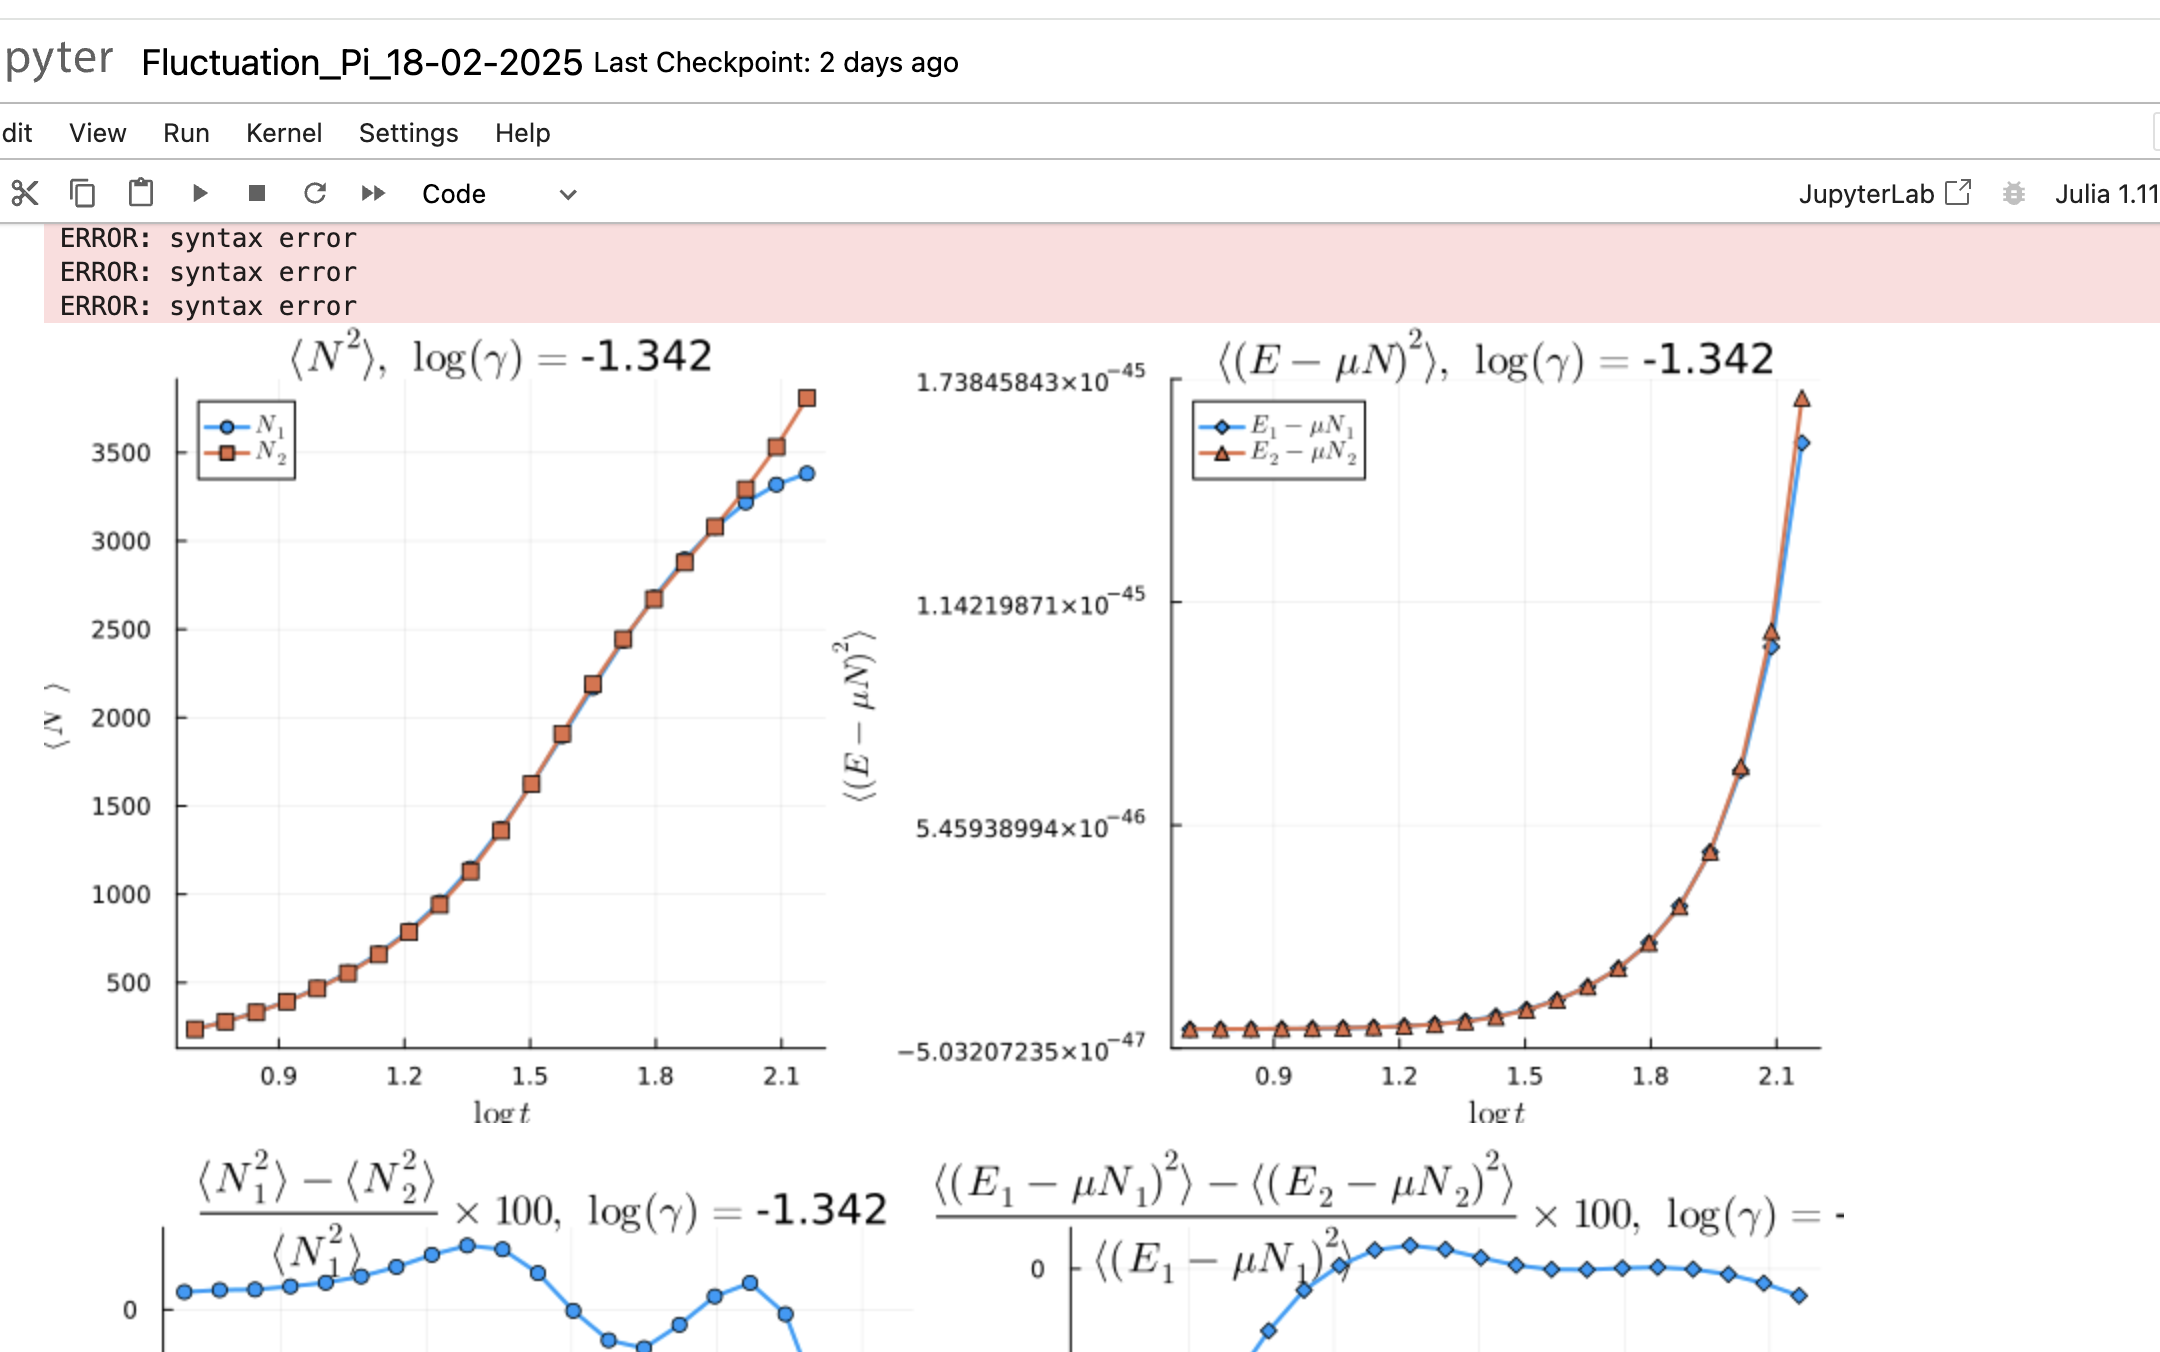
\includegraphics[width=1\textwidth]{Figures/test}

%\begin{aff}
%Donc une a l'ordre un en $\delta \theta (\operator{A}^{(0)})^{-1} %\operator{V}$ 

%\begin{eqnarray*}
%	\langle \delta \Pi ( \theta) \delta \Pi ( \theta') \rangle & = &  ( (\Pi^c_s - \Pi^c)\Pi^c/\Pi^c_s ) ( \theta ) \delta_{\theta, \theta'}/\delta \theta + \mathscr{F}(\theta , \theta' ) ,	
%\end{eqnarray*}

%avec 

%\begin{eqnarray*}
%	\mathscr{F}(\theta , \theta' ) & = & \left [ (\Pi^c_s - \Pi^c )( \theta)  +  (\Pi^c_s - \Pi^c ) ( \theta' )\right ] \frac{\Pi^c}{\Pi^c_s}(\theta)\frac{\Pi^c}{\Pi^c_s}(\theta') \frac{ \Delta( \theta'- \theta )}{ 2 \pi }\\
%	&&  - \left [ (\Pi^c_s - \Pi^c )( \theta)   (\Pi^c_s - \Pi^c ) ( \theta' )\right ] \frac{\Pi^c}{\Pi^c_s}(\theta)\frac{\Pi^c}{\Pi^c_s}(\theta')\int d\theta'' \left (   \frac{ \Pi^c/\Pi^c_s}{\Pi^c_s - \Pi^c} \right )(\theta'') \frac{\Delta(\theta''- \theta)}{2 \pi}\frac{\Delta(\theta''- \theta')}{2 \pi}  	
%\end{eqnarray*}
%\end{aff}



 











 
%\subsection{Fonction d’onde et Hamiltonien et moment à N corps}
%%Dans ce chapitre, nous nous intéressons aux fluctuations de la distribution de rapidité \( \delta \rho \) autour d'une distribution de référence \( \rho^c \), qui maximise la contribution à la fonction de partition des états, exprimée comme une fonctionnelle de la distribution \( \rho \) : 

La fonction de partition des états, s'exprime comme une fonctionnelle de la distribution \( \rho \) : 

\begin{eqnarray*}
	\Xi & = & \sum_\rho \exp \left( -\mathcal{A}(\rho) \right).
\end{eqnarray*}  

Dans la section {\em \bf Entropie de Yang-Yang} (\ref{??}), l'action \( \mathcal{A}(\rho) \) s'écrit sous la forme :  

\begin{eqnarray*}
	\mathcal{A}(\rho) & \doteq & - L\mathcal{S}_{YY}(\rho) + L\int f(\theta) \rho (\theta) \, d\theta,		
\end{eqnarray*}  

où \( \mathcal{S}_{YY} \) est la fonctionnelle d'entropie de Yang-Yang, définie dans (\ref{??}), et \( f \) est la fonction paramétrant les charges, introduite dans (\ref{??}).  

Dans cette même section {\em \bf Entropie de Yang-Yang} (\ref{??}), nous avons établi un lien entre \( f \) et distribution de référence \( \rho^c \), qui maximise la contribution à la fonction de partition des états .\\

On veux tester si nos experience est décrit pas un GGE. Pour cela nous nous intéressons aux fluctuations de la distribution de rapidité \( \delta \rho \) autour \( \rho^c \).

%Nous poursuivons à présent avec cette définition de l'action de classe $\mathcal{C}^2$ et admetant une distribution critique $\rho^c$ tel que sa différentielle en ce point critique soit nulle $d\mathcal{A}_{\rho^c} = 0 $ (\ref{??}) de sorte que d'aprés la formule de Taylor-Youg %afin de déterminer les fluctuations autour de \( \Pi^c \). Pour cela, nous réécrivons l'action sous la forme :  

Nous poursuivons à présent avec cette définition de l'action de classe $\mathcal{C}^2$ et admetant une distribution critique $\rho^c$ tel que sa différentielle en ce point critique soit nulle $d\mathcal{A}_{\rho^c} = 0 $ (\ref{??}) de sorte que d'aprés la formule de Taylor-Youg %afin de déterminer les fluctuations autour de \( \Pi^c \). Pour cela, nous réécrivons l'action sous la forme :  

\begin{eqnarray*}  
	\mathcal{A}(\rho^c + \delta \rho) & \underset{ \delta \rho \to 0 }{=} & \mathcal{A}(\rho^c)  + \frac{1}{2} \left. \frac{\delta^2 \mathcal{A}}{\delta \rho^2} \right|_{\rho^c} (\delta \rho) + \mathcal{O}((\delta \rho)^3),  
\end{eqnarray*}  

une expression quadratique pour l'action à l'ordre dominant en \( \delta \Pi \) avec $\left. \frac{\delta^2 \mathcal{A}}{\delta \rho^2} \right|_{\rho^c}$ la forme quadratique définie positive (Fig (\ref{fig.fluctu.A})).

\begin{figure}[H]
	\centering 
	\begin{tikzpicture}
		\begin{scope}[shift={(0,0)}]
			\begin{scope}[transform canvas={scale=0.6}]
				% Définition des couleurs avec les codes HTML
\definecolor{colorOne}{HTML}{443E46}
\definecolor{colorTwo}{HTML}{F6DEB8}
\definecolor{colorThree}{HTML}{908CA4}
\definecolor{colorFour}{HTML}{57659E}
\definecolor{colorFive}{HTML}{C57284}
\definecolor{colorSix}{HTML}{FF5B69}

% Raccourcis pour les couleurs
\def\colorOne{colorOne}
\def\colorTwo{colorTwo}
\def\colorThree{colorThree}
\def\colorFour{colorFour}
\def\colorFive{colorFive}
\def\colorSix{colorSix}

\def\colorslide{blue!50!black}



\begin{scope}
	% Tracer une courbe lisse entre des points
	\draw[shift={(0,0)} ,\colorOne]
		(-1 , 0 ) edge [thick,line width=0.8ex , ->,>=triangle 45  , \colorOne] node [pos = 1 , below ]{\huge$\rho$}( 5  , 0 )
	;
	\draw[shift={(0,0)}, color=\colorOne]
		(0, -1.0 ) edge [thick,line width=0.8ex , ->,>=triangle 45  ]node [pos=0.9,left=0.2cm ]{\huge$\mathcal{A}(\rho)$}( 0  , 5 )
	;
	\draw[]
		(2.5, 0.12 ) edge [thick,line width=0.8ex ,\colorThree ]node [pos=1,below  ]{\huge$\rho^c$} (2.5, -0.12 )	
	;
	
	\draw[]
		(2.5, -0.12 ) edge [thick,line width=0.4ex , dashed, \colorThree ] (2.5, 5.5 )
		(1.5, 1 ) edge [thick,line width=0.4ex , <->,>=triangle 45  , \colorThree ] (3.5, 1 )
		(-0.3,1) edge [thick,line width=0.4ex  , \colorThree ] node [pos=0,left ]{\huge$\mathcal{A}(\rho^c)$} (0.3, 1 )	
	;
    \draw[thick, line width=0.8ex , \colorFour] plot[smooth, tension=0.7] coordinates {
        (1, 5) (1.6 , 3 ) (2.5, 1) (3.5 , 3 )  (4, 5)
    };		
	
\end{scope}

	
			
			\end{scope}
			
			\draw[color = red , scale = 0.5 , draw = none  ] (-2 , -1) rectangle (5, 6) ; 	
		\end{scope}
		
		\begin{scope}[shift={(19,-1)}]
			\begin{scope}[transform canvas={scale=0.6}]
				% Définition des couleurs avec les codes HTML
\definecolor{colorOne}{HTML}{443E46}
\definecolor{colorTwo}{HTML}{F6DEB8}
\definecolor{colorThree}{HTML}{908CA4}
\definecolor{colorFour}{HTML}{57659E}
\definecolor{colorFive}{HTML}{C57284}
\definecolor{colorSix}{HTML}{FF5B69}

% Raccourcis pour les couleurs
\def\colorOne{colorOne}
\def\colorTwo{colorTwo}
\def\colorThree{colorThree}
\def\colorFour{colorFour}
\def\colorFive{colorFive}
\def\colorSix{colorSix}

\def\colorslide{blue!50!black}

\def\Occupation{
	\def\traitx{0.3}
	\def\traity{0.5}
	\draw[shift={(0,0)}]
		(-13.5 , 0 ) edge [thick,line width=0.8ex ]( -3.2  , 0 )
		( -3.2 - \traitx  , 0 - \traity ) edge [thick,line width=0.8ex ]( -3.2 + \traitx  , 0 + \traity  )
		( -2.8 - \traitx  , 0 - \traity ) edge [thick,line width=0.8ex ]( -2.8 + \traitx  , 0 + \traity  )
		(-2.8 , 0 ) edge [thick,line width=0.8ex ](2.8  , 0 )
		( 2.8 - \traitx  , 0 - \traity ) edge [thick,line width=0.8ex ]( 2.8 + \traitx  , 0 + \traity  )
		( 3.2 - \traitx  , 0 - \traity ) edge [thick,line width=0.8ex ]( 3.2 + \traitx  , 0 + \traity  )
		(3.2, 0 ) edge [thick,line width=0.8ex,->,>=triangle 45 , color = black ]node [pos=1.01,below  ]{\huge$\theta$}	( 13  , 0 )
	;
	\draw[shift={(0,0)}, color=\colorOne]
		(-10.5 , -1.5 ) edge [thick,line width=0.8ex , ->,>=triangle 45  ]( -10.5  , 4.5 )
	;
		
	\foreach \r in {1 , ... , 3 } {
%		\draw[
%		decoration={
%		markings,
%    	mark connection node=my node,
%    	mark=at position 0 with{\node [blue,transform shape] (my node) {\large \r};}},
%		color=gray, thick, 
%		line width=0.5ex] decorate { 
%            (-11.0, \r) -- (-10.1, \r )}
%        ;
        \draw[
			color=\colorOne,
			] 
            (-11.0, \r) edge[color=\colorThree , thick,line width=0.5ex] node [pos=-0.5 ]{\large\color{\colorFour} $\frac{\r}{\delta \theta}$ } (-10.3, \r )
        	;
	
	}
	

	
	% Graduation abcsisse 
	% Définitions des listes
% Definitions of the lists
\def\listetuple{-9/\theta_{1}, -8/\theta_{2} , -5/\theta_{3} , -2/\theta_{a-1} , 0/\theta_{a} , 1/\theta_{a+1} , 2/\theta_{a+2} ,  5/\theta_{N-4} , 7/\theta_{N-3},8/\theta_{N-1},9/\theta_{N} }
\def\listetrais{-12 , -11, -10, -9 , -8 , -7 ,  -6 , -5, -4.5,-4, -2 , -1, 0 , 0.5, 1, 2, 4 , 5 ,  6 , 7 , 8 ,8.5, 9 ,  10 , 11, 12 }

% Loop over listetrais
\foreach \r in \listetrais {
    % Initialize found variable to zero
    % Initialize found variable to zero
    %\pgfmathsetmacro\found{0}
    \global\def\found{0}
    \xdef\nomtheta{}
    
    % Check if \r is in listetuple
    \foreach \x/\y in \listetuple { 
        \ifdim \r pt=\x pt % If \r matches any \x in listetuple
            \global\def\found{1} ;
            \xdef\nomtheta{\y} % Set \nomtheta to the corresponding \y
            %\pgfmathsetmacro\found{1} % Set found to 1            
            %\global\pgfmathsetmacro\found{1}
        \fi
    }
    
    %\node [circle, draw, red] (A) at (\r, 2) {\found , $\nomtheta$};
    
    % Draw the line and display \nomtheta if found
    \ifnum\found=1
        \draw[color=\colorOne, thick, line width=0.5ex] 
            (\r, -0.3) -- (\r, 0.3) node[red , pos=-0.5] {\large $\nomtheta$};
         \filldraw[line width=0.5ex, color=\colorSix, outer color=\colorSix, inner color=\colorSix] 
            (\r, 0) circle (4pt);
    \else 
        % Draw without \nomtheta and add a blue circle if not found
        \draw[color=\colorOne, thick, line width=0.5ex] 
            (\r, -0.3) -- (\r, 0.3);
        \filldraw[line width=0.5ex, color=\colorSix, outer color=\colorTwo, inner color=\colorTwo] 
            (\r, 0) circle (4pt); 
    \fi
}

\def\listetrais{-9.5/\theta_{i-1}/2/3, -6.5/\theta_{i}/1/4  ,   -1.5/\theta_{j}/2/4 , 1.5/\theta_{j+1}/-1/3 , 3.5/\theta_{\ell-1}/1/3 , 6.5/\theta_{\ell}/3/4 , 9.5/\theta(\theta_{\ell+1})/-1/3 };



\foreach \r/\nomx/\y/\ys in \listetrais {
	\draw[
		decoration={
		markings,
    	mark connection node=my node,
    	mark=at position .5 with{\node [blue,transform shape] (my node) {\large \color{\colorFour} $\nomx$};}},
		color=\colorThree , thick, 
		line width=0.5ex] decorate { 
            (\r, 0.12) -- (\r, -1.2)}
        ;
     
     \ifdim \y pt > -1 pt 
     	\draw[
			decoration={
			markings,
    		mark connection node=my node,
    		mark=at position .5 with{\node [blue,transform shape] (my node) {\large \color{\colorFour} $\Pi(\nomx) $};}},
			color=\colorThree, thick, 
			line width=0.5ex] decorate { 
            (\r, \y) -- (\r +3, \y)}
        ;
        \draw[
			decoration={
			markings,
    		mark connection node=my node,
    		mark=at position .5 with{\node [blue,transform shape] (my node) {\large \color{\colorFive} $\Pi_s(\nomx) $};}},
			color=\colorFive, thick, 
			line width=0.5ex] decorate { 
            (\r, \ys) -- (\r +3, \ys)}
        ;
     \fi 
     \ifdim \r pt= -1.5 pt
     	\draw[
     		decoration={
			markings,
    		mark connection node=my node,
    		mark=at position .5 with{\node [blue,transform shape] (my node) {\large \color{\colorFour}  $\delta \theta $};},
    		%mark=at position 0.1  with {\arrow[blue, line width=0.5ex]{<}},
    		%mark=at position 1  with {\arrow[blue, line width=0.5ex]{>}}
    		},
        	color=\colorThree,
        	thick,
        	line width=0.5ex,
        	%arrows={Computer Modern Rightarrow[line cap=round]-Computer Modern Rightarrow[line cap=round]}
   			](\r, -1.2) edge[arrows={Computer Modern Rightarrow[line cap=round]-}] (\r + 0.4, -1.2)decorate {
    		(\r, -1.2) -- (\r + 3, -1.2)}(\r + 2, -1.2) edge[arrows={-Computer Modern Rightarrow[line cap=round]}] (\r + 3, -1.2)
    		;
    \fi
			
	
}


			
}


\begin{scope}
	%\draw[help lines , width=1.5ex] (-8,-3) grid (8,3);\draw[help lines ,width=0.5ex , opacity = 0.5] (-3,-3) grid[step=0.1] (3,3));
	
	%\draw[help lines] 
	%	(-3,-3) edge[width=1.5ex] grid (3,3)	
	%	(-3,-3) edge[width=0.5ex , opacity = 0.5] grid (3,3)	
	%;
	\begin{scope}[shift={(0,1)},rotate=0,opacity=1,color=black]
		\Occupation	
		
		%\node[anchor=east, font=\bfseries] at (-11, 0) {\color{red}\large (T = 0 )} ;	
	\end{scope}
	
	
	
	
	\begin{scope}[shift={(-10.5,7)},rotate=0,opacity=1,color=black]
	
	\begin{scope}[shift={(-0,0)},rotate=0,opacity=1,color=black]
	
		\draw[shift={(0,0)} ,line width=1ex,rounded corners = 1ex,color=\colorOne , opacity =1 ,fill=\colorOne!00 , pattern={north east lines} , pattern color=\colorOne!00 ]
			(0 , -1 ) rectangle (5,1)
		;
		

		\begin{scope}[shift={(0.5,0.5)}]
			\draw[color=\colorOne, thick, line width=0.5ex] 
            (0, -0.3) -- (0, 0.3) ;
            \filldraw[line width=0.5ex, color=\colorSix, outer color=\colorSix, inner color=\colorSix] 
            (0, 0) circle (4pt);
            
            \node[anchor=west, font=\bfseries] at (0.2, 0) {\color{\colorSix}\large : quasi-particule};
		\end{scope}
		
		\begin{scope}[shift={(0.5,-0.5)}]
			\draw[color=\colorOne, thick, line width=0.5ex] 
            (0, -0.3) -- (0, 0.3) ;
            \filldraw[line width=0.5ex, color=\colorSix, outer color=\colorTwo, inner color=\colorTwo] 
            (0, 0) circle (4pt);
            
            \node[anchor=west, font=\bfseries] at (0.2, 0) {\color{\colorSix}\large : hole};
		\end{scope}

	\end{scope}
	
	\begin{scope}[shift={(6,0)},rotate=0,opacity=1,color=black]	
		
		\draw[shift={(0,0)} ,line width=1ex,rounded corners = 1ex,color=\colorOne , opacity =1 ,fill=\colorOne!00 , pattern={north east lines} , pattern color=\colorOne!00 ]
			(0 , -1 ) rectangle (7.5,1)
		;
		
		\node[anchor=west] at (0.5, 0.5) {\color{\colorFour}\large $\Pi$ };\node[anchor=west, font=\bfseries] at (1, 0.5) {\color{\colorFour}\large : quasi-particule distribution};
		
		\node[anchor=west] at (0.5, -0.5) {\color{\colorFour}\large $\Pi_h$ };\node[anchor=west, font=\bfseries] at (1, -0.5) {\color{\colorFour}\large  : hole distribution};
		
	\end{scope}
	
	\begin{scope}[shift={(14.5,0)},rotate=0,opacity=1,color=black]	
		
		\draw[shift={(0,0)} ,line width=1ex,rounded corners = 1ex,color=\colorOne , opacity =1 ,fill=\colorOne!00 , pattern={north east lines} , pattern color=\colorOne!00 ]
			(0 , -0.5 ) rectangle (7.0,0.5)
		;
		
		\node[anchor=west] at (0.2, 0) {\color{\colorFour}\large ${\color{\colorFive}\Pi_s} = \Pi + \Pi_h $ } node[anchor=west , font=\bfseries] at (3.1 , 0 )  {\color{\colorFour}\large {\color{\colorFive} : density of states}};
		
	\end{scope}
	
	
	\end{scope}


		
	
\end{scope}

	
			
			\end{scope}
			\begin{scope}[scale=1]
				\draw[color = red , scale = 1 , draw = none  ] (-1 , -1) rectangle (5, 5) ; 
			\end{scope}	
		\end{scope}

		
				
			
	\end{tikzpicture}	
	\captionsetup{skip=10pt} % Ajoute de l’espace après la légende
	\label{fig.fluctu.A}
\end{figure}


On discrétise l'axe des rapidités en  petite cellule de rapidité $[\theta, \theta+\delta\theta]$, qui contient $L\rho(\theta) \delta \theta$ rapidités. 
	



Avec ces petites tranches, la forme quadratique s’écrit :

\begin{eqnarray*}
    \left. \frac{\delta^2 \mathcal{A}}{{\delta \rho}^2} \right|_{\rho^c}(\delta \rho ) &=&  \sum_{a,b \mid \text{tranche}}  
    \delta \rho(\theta_a)  \frac{\partial^2 \mathcal{A}}{\partial \delta \rho(\theta_a) \partial \delta \rho(\theta_b) } (\rho^c)  \delta \rho(\theta_b).
\end{eqnarray*}
Les fluctuations s’écrivent donc :

\begin{eqnarray*}
    \langle \delta \rho ( \theta) \delta \rho ( \theta') \rangle &=&  
    \frac{ \int d\delta \rho \, \delta \rho(\theta) \delta \rho ( \theta') 
    \exp \left( - \frac{1}{2} \sum_{a,b \mid \text{tranche}}  
    \delta \rho(\theta_a) \frac{\partial^2 \mathcal{A}}{\partial \delta \rho(\theta_a) \partial \delta \rho(\theta_b) } (\rho^c)  \delta \rho(\theta_b) \right) }
    { \int d\delta \Pi  
    \exp \left( - \frac{1}{2} \sum_{a,b \mid \text{tranche}}  
    \delta \rho(\theta_a) \frac{\partial^2 \mathcal{A}}{\partial \delta \rho(\theta_a) \partial \delta \rho(\theta_b) } (\rho^c)  \delta \rho(\theta_b) \right) } \\
    &=& \left( \mathbf{A}^{-1} \right)_{\theta , \theta'}
\end{eqnarray*}


\begin{aff}

\begin{eqnarray*}
	\langle \delta \rho ( \theta) \delta \rho ( \theta') \rangle &=& 	\left( \mathbf{A}^{-1} \right)_{\theta , \theta'}
\end{eqnarray*}

	
avec la  {\em matrice hessienne} $\mathbf{A}_{\theta , \theta'} \equiv \frac{\partial^2 \mathcal{A}}{\partial \delta \rho(\theta) \partial \delta \rho(\theta') }(\rho^c)$, au point critique/ qui maximise la probabilité  $\rho^c=\rho^c_s \nu^c $, s'écrit

\begin{eqnarray*}
	\operator{A} & = & \operator{A}^{(0)} + \delta \theta \operator{V}
\end{eqnarray*}

avec 

\begin{eqnarray*}
	A^{(0)}_{\theta , \theta'}  & = &  L\delta \theta \left ( \frac{ 1}{\rho^c_s ( 1  - \nu^c ) \nu^c } \right )(\theta)    \delta({\theta - \theta '})	,\\
	V_{\theta , \theta'}  &= & L \delta \theta \left \{ - \left [ \left ( \frac{1}{\rho^c_s( 1 - \nu^c) } \right ) ( \theta)  +  \left ( \frac{1}{\rho^c_s( 1 - \nu^c) } \right ) ( \theta' )\right ] \frac{ \Delta( \theta'- \theta )}{ 2 \pi } + \int d\theta''  \left ( \frac{\nu^c}{\rho^c_s( 1 - \nu^c) } \right )(\theta'') \frac{\Delta(\theta''- \theta)}{2 \pi}\frac{\Delta(\theta''- \theta')}{2 \pi}   \right \} 	
\end{eqnarray*}

\end{aff}

\subsection{Testes}

\begin{eqnarray*}
	\Delta_{\operator{\mathcal{N}}}^2  & = &  \frac{1}{\beta} \left . \frac{\partial \langle \operator{\mathcal{N}} \rangle}{\partial \mu} \right )_T \\
	\Delta_{\operator{\mathcal{E}}-\mu \operator{\mathcal{N}}}^2  & = &  - \left . \frac{\partial \langle \operator{\mathcal{E}}-\mu \operator{\mathcal{N}} \rangle}{\partial \beta} \right )_\mu 
\end{eqnarray*}

et 

\begin{eqnarray*}
	\Delta_{\operator{\mathcal{N}}}^2  &= & L^2 \int d\theta_a \int d \theta_b \, \langle \delta \rho(\theta_a) \delta \rho(\theta_b) \rangle \\
	\Delta_{\operator{\mathcal{E}}-\mu \operator{\mathcal{N}}}^2  & = & L^2 \int d\theta_a \int d \theta_b \, \left ( - \mu + \frac{1}2 m \theta_a^2  \right  )\left ( - \mu + \frac{1}2 m \theta_b^2  \right  )  \langle \delta \rho(\theta_a) \delta \rho(\theta_b) \rangle
\end{eqnarray*}

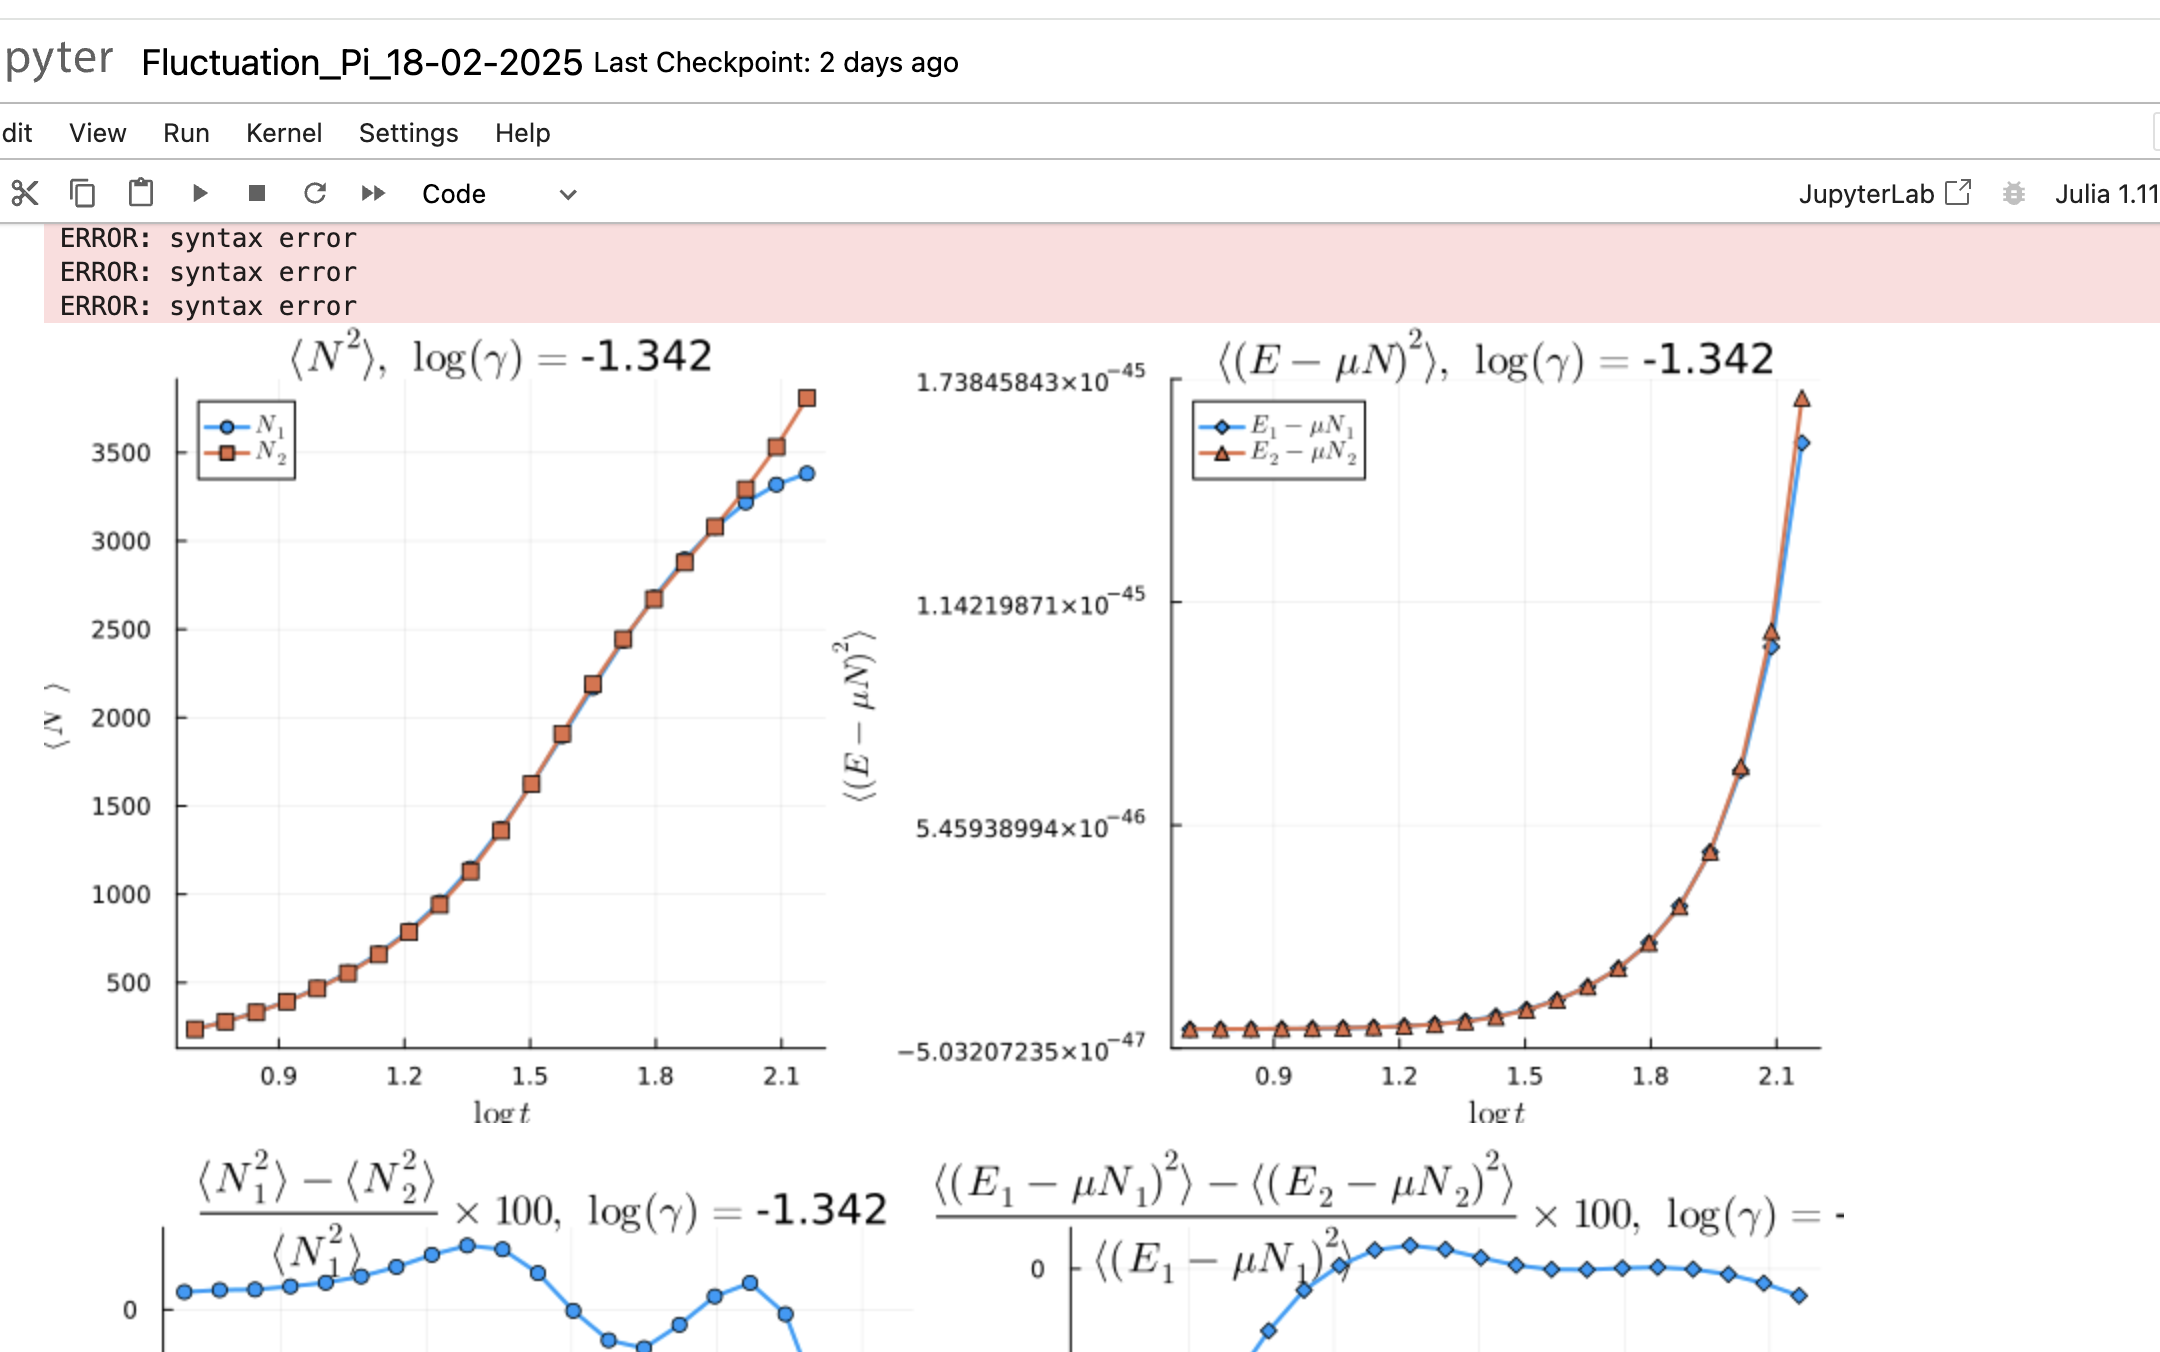
\includegraphics[width=1\textwidth]{Figures/test}

%\begin{aff}
%Donc une a l'ordre un en $\delta \theta (\operator{A}^{(0)})^{-1} %\operator{V}$ 

%\begin{eqnarray*}
%	\langle \delta \Pi ( \theta) \delta \Pi ( \theta') \rangle & = &  ( (\Pi^c_s - \Pi^c)\Pi^c/\Pi^c_s ) ( \theta ) \delta_{\theta, \theta'}/\delta \theta + \mathscr{F}(\theta , \theta' ) ,	
%\end{eqnarray*}

%avec 

%\begin{eqnarray*}
%	\mathscr{F}(\theta , \theta' ) & = & \left [ (\Pi^c_s - \Pi^c )( \theta)  +  (\Pi^c_s - \Pi^c ) ( \theta' )\right ] \frac{\Pi^c}{\Pi^c_s}(\theta)\frac{\Pi^c}{\Pi^c_s}(\theta') \frac{ \Delta( \theta'- \theta )}{ 2 \pi }\\
%	&&  - \left [ (\Pi^c_s - \Pi^c )( \theta)   (\Pi^c_s - \Pi^c ) ( \theta' )\right ] \frac{\Pi^c}{\Pi^c_s}(\theta)\frac{\Pi^c}{\Pi^c_s}(\theta')\int d\theta'' \left (   \frac{ \Pi^c/\Pi^c_s}{\Pi^c_s - \Pi^c} \right )(\theta'') \frac{\Delta(\theta''- \theta)}{2 \pi}\frac{\Delta(\theta''- \theta')}{2 \pi}  	
%\end{eqnarray*}
%\end{aff}



 








%\subsection{Introduction au modèle de gaz de Bose unidimensionnel}
%Dans ce chapitre, nous nous intéressons aux fluctuations de la distribution de rapidité \( \delta \rho \) autour d'une distribution de référence \( \rho^c \), qui maximise la contribution à la fonction de partition des états, exprimée comme une fonctionnelle de la distribution \( \rho \) : 

La fonction de partition des états, s'exprime comme une fonctionnelle de la distribution \( \rho \) : 

\begin{eqnarray*}
	\Xi & = & \sum_\rho \exp \left( -\mathcal{A}(\rho) \right).
\end{eqnarray*}  

Dans la section {\em \bf Entropie de Yang-Yang} (\ref{??}), l'action \( \mathcal{A}(\rho) \) s'écrit sous la forme :  

\begin{eqnarray*}
	\mathcal{A}(\rho) & \doteq & - L\mathcal{S}_{YY}(\rho) + L\int f(\theta) \rho (\theta) \, d\theta,		
\end{eqnarray*}  

où \( \mathcal{S}_{YY} \) est la fonctionnelle d'entropie de Yang-Yang, définie dans (\ref{??}), et \( f \) est la fonction paramétrant les charges, introduite dans (\ref{??}).  

Dans cette même section {\em \bf Entropie de Yang-Yang} (\ref{??}), nous avons établi un lien entre \( f \) et distribution de référence \( \rho^c \), qui maximise la contribution à la fonction de partition des états .\\

On veux tester si nos experience est décrit pas un GGE. Pour cela nous nous intéressons aux fluctuations de la distribution de rapidité \( \delta \rho \) autour \( \rho^c \).

%Nous poursuivons à présent avec cette définition de l'action de classe $\mathcal{C}^2$ et admetant une distribution critique $\rho^c$ tel que sa différentielle en ce point critique soit nulle $d\mathcal{A}_{\rho^c} = 0 $ (\ref{??}) de sorte que d'aprés la formule de Taylor-Youg %afin de déterminer les fluctuations autour de \( \Pi^c \). Pour cela, nous réécrivons l'action sous la forme :  

Nous poursuivons à présent avec cette définition de l'action de classe $\mathcal{C}^2$ et admetant une distribution critique $\rho^c$ tel que sa différentielle en ce point critique soit nulle $d\mathcal{A}_{\rho^c} = 0 $ (\ref{??}) de sorte que d'aprés la formule de Taylor-Youg %afin de déterminer les fluctuations autour de \( \Pi^c \). Pour cela, nous réécrivons l'action sous la forme :  

\begin{eqnarray*}  
	\mathcal{A}(\rho^c + \delta \rho) & \underset{ \delta \rho \to 0 }{=} & \mathcal{A}(\rho^c)  + \frac{1}{2} \left. \frac{\delta^2 \mathcal{A}}{\delta \rho^2} \right|_{\rho^c} (\delta \rho) + \mathcal{O}((\delta \rho)^3),  
\end{eqnarray*}  

une expression quadratique pour l'action à l'ordre dominant en \( \delta \Pi \) avec $\left. \frac{\delta^2 \mathcal{A}}{\delta \rho^2} \right|_{\rho^c}$ la forme quadratique définie positive (Fig (\ref{fig.fluctu.A})).

\begin{figure}[H]
	\centering 
	\begin{tikzpicture}
		\begin{scope}[shift={(0,0)}]
			\begin{scope}[transform canvas={scale=0.6}]
				% Définition des couleurs avec les codes HTML
\definecolor{colorOne}{HTML}{443E46}
\definecolor{colorTwo}{HTML}{F6DEB8}
\definecolor{colorThree}{HTML}{908CA4}
\definecolor{colorFour}{HTML}{57659E}
\definecolor{colorFive}{HTML}{C57284}
\definecolor{colorSix}{HTML}{FF5B69}

% Raccourcis pour les couleurs
\def\colorOne{colorOne}
\def\colorTwo{colorTwo}
\def\colorThree{colorThree}
\def\colorFour{colorFour}
\def\colorFive{colorFive}
\def\colorSix{colorSix}

\def\colorslide{blue!50!black}



\begin{scope}
	% Tracer une courbe lisse entre des points
	\draw[shift={(0,0)} ,\colorOne]
		(-1 , 0 ) edge [thick,line width=0.8ex , ->,>=triangle 45  , \colorOne] node [pos = 1 , below ]{\huge$\rho$}( 5  , 0 )
	;
	\draw[shift={(0,0)}, color=\colorOne]
		(0, -1.0 ) edge [thick,line width=0.8ex , ->,>=triangle 45  ]node [pos=0.9,left=0.2cm ]{\huge$\mathcal{A}(\rho)$}( 0  , 5 )
	;
	\draw[]
		(2.5, 0.12 ) edge [thick,line width=0.8ex ,\colorThree ]node [pos=1,below  ]{\huge$\rho^c$} (2.5, -0.12 )	
	;
	
	\draw[]
		(2.5, -0.12 ) edge [thick,line width=0.4ex , dashed, \colorThree ] (2.5, 5.5 )
		(1.5, 1 ) edge [thick,line width=0.4ex , <->,>=triangle 45  , \colorThree ] (3.5, 1 )
		(-0.3,1) edge [thick,line width=0.4ex  , \colorThree ] node [pos=0,left ]{\huge$\mathcal{A}(\rho^c)$} (0.3, 1 )	
	;
    \draw[thick, line width=0.8ex , \colorFour] plot[smooth, tension=0.7] coordinates {
        (1, 5) (1.6 , 3 ) (2.5, 1) (3.5 , 3 )  (4, 5)
    };		
	
\end{scope}

	
			
			\end{scope}
			
			\draw[color = red , scale = 0.5 , draw = none  ] (-2 , -1) rectangle (5, 6) ; 	
		\end{scope}
		
		\begin{scope}[shift={(19,-1)}]
			\begin{scope}[transform canvas={scale=0.6}]
				% Définition des couleurs avec les codes HTML
\definecolor{colorOne}{HTML}{443E46}
\definecolor{colorTwo}{HTML}{F6DEB8}
\definecolor{colorThree}{HTML}{908CA4}
\definecolor{colorFour}{HTML}{57659E}
\definecolor{colorFive}{HTML}{C57284}
\definecolor{colorSix}{HTML}{FF5B69}

% Raccourcis pour les couleurs
\def\colorOne{colorOne}
\def\colorTwo{colorTwo}
\def\colorThree{colorThree}
\def\colorFour{colorFour}
\def\colorFive{colorFive}
\def\colorSix{colorSix}

\def\colorslide{blue!50!black}

\def\Occupation{
	\def\traitx{0.3}
	\def\traity{0.5}
	\draw[shift={(0,0)}]
		(-13.5 , 0 ) edge [thick,line width=0.8ex ]( -3.2  , 0 )
		( -3.2 - \traitx  , 0 - \traity ) edge [thick,line width=0.8ex ]( -3.2 + \traitx  , 0 + \traity  )
		( -2.8 - \traitx  , 0 - \traity ) edge [thick,line width=0.8ex ]( -2.8 + \traitx  , 0 + \traity  )
		(-2.8 , 0 ) edge [thick,line width=0.8ex ](2.8  , 0 )
		( 2.8 - \traitx  , 0 - \traity ) edge [thick,line width=0.8ex ]( 2.8 + \traitx  , 0 + \traity  )
		( 3.2 - \traitx  , 0 - \traity ) edge [thick,line width=0.8ex ]( 3.2 + \traitx  , 0 + \traity  )
		(3.2, 0 ) edge [thick,line width=0.8ex,->,>=triangle 45 , color = black ]node [pos=1.01,below  ]{\huge$\theta$}	( 13  , 0 )
	;
	\draw[shift={(0,0)}, color=\colorOne]
		(-10.5 , -1.5 ) edge [thick,line width=0.8ex , ->,>=triangle 45  ]( -10.5  , 4.5 )
	;
		
	\foreach \r in {1 , ... , 3 } {
%		\draw[
%		decoration={
%		markings,
%    	mark connection node=my node,
%    	mark=at position 0 with{\node [blue,transform shape] (my node) {\large \r};}},
%		color=gray, thick, 
%		line width=0.5ex] decorate { 
%            (-11.0, \r) -- (-10.1, \r )}
%        ;
        \draw[
			color=\colorOne,
			] 
            (-11.0, \r) edge[color=\colorThree , thick,line width=0.5ex] node [pos=-0.5 ]{\large\color{\colorFour} $\frac{\r}{\delta \theta}$ } (-10.3, \r )
        	;
	
	}
	

	
	% Graduation abcsisse 
	% Définitions des listes
% Definitions of the lists
\def\listetuple{-9/\theta_{1}, -8/\theta_{2} , -5/\theta_{3} , -2/\theta_{a-1} , 0/\theta_{a} , 1/\theta_{a+1} , 2/\theta_{a+2} ,  5/\theta_{N-4} , 7/\theta_{N-3},8/\theta_{N-1},9/\theta_{N} }
\def\listetrais{-12 , -11, -10, -9 , -8 , -7 ,  -6 , -5, -4.5,-4, -2 , -1, 0 , 0.5, 1, 2, 4 , 5 ,  6 , 7 , 8 ,8.5, 9 ,  10 , 11, 12 }

% Loop over listetrais
\foreach \r in \listetrais {
    % Initialize found variable to zero
    % Initialize found variable to zero
    %\pgfmathsetmacro\found{0}
    \global\def\found{0}
    \xdef\nomtheta{}
    
    % Check if \r is in listetuple
    \foreach \x/\y in \listetuple { 
        \ifdim \r pt=\x pt % If \r matches any \x in listetuple
            \global\def\found{1} ;
            \xdef\nomtheta{\y} % Set \nomtheta to the corresponding \y
            %\pgfmathsetmacro\found{1} % Set found to 1            
            %\global\pgfmathsetmacro\found{1}
        \fi
    }
    
    %\node [circle, draw, red] (A) at (\r, 2) {\found , $\nomtheta$};
    
    % Draw the line and display \nomtheta if found
    \ifnum\found=1
        \draw[color=\colorOne, thick, line width=0.5ex] 
            (\r, -0.3) -- (\r, 0.3) node[red , pos=-0.5] {\large $\nomtheta$};
         \filldraw[line width=0.5ex, color=\colorSix, outer color=\colorSix, inner color=\colorSix] 
            (\r, 0) circle (4pt);
    \else 
        % Draw without \nomtheta and add a blue circle if not found
        \draw[color=\colorOne, thick, line width=0.5ex] 
            (\r, -0.3) -- (\r, 0.3);
        \filldraw[line width=0.5ex, color=\colorSix, outer color=\colorTwo, inner color=\colorTwo] 
            (\r, 0) circle (4pt); 
    \fi
}

\def\listetrais{-9.5/\theta_{i-1}/2/3, -6.5/\theta_{i}/1/4  ,   -1.5/\theta_{j}/2/4 , 1.5/\theta_{j+1}/-1/3 , 3.5/\theta_{\ell-1}/1/3 , 6.5/\theta_{\ell}/3/4 , 9.5/\theta(\theta_{\ell+1})/-1/3 };



\foreach \r/\nomx/\y/\ys in \listetrais {
	\draw[
		decoration={
		markings,
    	mark connection node=my node,
    	mark=at position .5 with{\node [blue,transform shape] (my node) {\large \color{\colorFour} $\nomx$};}},
		color=\colorThree , thick, 
		line width=0.5ex] decorate { 
            (\r, 0.12) -- (\r, -1.2)}
        ;
     
     \ifdim \y pt > -1 pt 
     	\draw[
			decoration={
			markings,
    		mark connection node=my node,
    		mark=at position .5 with{\node [blue,transform shape] (my node) {\large \color{\colorFour} $\Pi(\nomx) $};}},
			color=\colorThree, thick, 
			line width=0.5ex] decorate { 
            (\r, \y) -- (\r +3, \y)}
        ;
        \draw[
			decoration={
			markings,
    		mark connection node=my node,
    		mark=at position .5 with{\node [blue,transform shape] (my node) {\large \color{\colorFive} $\Pi_s(\nomx) $};}},
			color=\colorFive, thick, 
			line width=0.5ex] decorate { 
            (\r, \ys) -- (\r +3, \ys)}
        ;
     \fi 
     \ifdim \r pt= -1.5 pt
     	\draw[
     		decoration={
			markings,
    		mark connection node=my node,
    		mark=at position .5 with{\node [blue,transform shape] (my node) {\large \color{\colorFour}  $\delta \theta $};},
    		%mark=at position 0.1  with {\arrow[blue, line width=0.5ex]{<}},
    		%mark=at position 1  with {\arrow[blue, line width=0.5ex]{>}}
    		},
        	color=\colorThree,
        	thick,
        	line width=0.5ex,
        	%arrows={Computer Modern Rightarrow[line cap=round]-Computer Modern Rightarrow[line cap=round]}
   			](\r, -1.2) edge[arrows={Computer Modern Rightarrow[line cap=round]-}] (\r + 0.4, -1.2)decorate {
    		(\r, -1.2) -- (\r + 3, -1.2)}(\r + 2, -1.2) edge[arrows={-Computer Modern Rightarrow[line cap=round]}] (\r + 3, -1.2)
    		;
    \fi
			
	
}


			
}


\begin{scope}
	%\draw[help lines , width=1.5ex] (-8,-3) grid (8,3);\draw[help lines ,width=0.5ex , opacity = 0.5] (-3,-3) grid[step=0.1] (3,3));
	
	%\draw[help lines] 
	%	(-3,-3) edge[width=1.5ex] grid (3,3)	
	%	(-3,-3) edge[width=0.5ex , opacity = 0.5] grid (3,3)	
	%;
	\begin{scope}[shift={(0,1)},rotate=0,opacity=1,color=black]
		\Occupation	
		
		%\node[anchor=east, font=\bfseries] at (-11, 0) {\color{red}\large (T = 0 )} ;	
	\end{scope}
	
	
	
	
	\begin{scope}[shift={(-10.5,7)},rotate=0,opacity=1,color=black]
	
	\begin{scope}[shift={(-0,0)},rotate=0,opacity=1,color=black]
	
		\draw[shift={(0,0)} ,line width=1ex,rounded corners = 1ex,color=\colorOne , opacity =1 ,fill=\colorOne!00 , pattern={north east lines} , pattern color=\colorOne!00 ]
			(0 , -1 ) rectangle (5,1)
		;
		

		\begin{scope}[shift={(0.5,0.5)}]
			\draw[color=\colorOne, thick, line width=0.5ex] 
            (0, -0.3) -- (0, 0.3) ;
            \filldraw[line width=0.5ex, color=\colorSix, outer color=\colorSix, inner color=\colorSix] 
            (0, 0) circle (4pt);
            
            \node[anchor=west, font=\bfseries] at (0.2, 0) {\color{\colorSix}\large : quasi-particule};
		\end{scope}
		
		\begin{scope}[shift={(0.5,-0.5)}]
			\draw[color=\colorOne, thick, line width=0.5ex] 
            (0, -0.3) -- (0, 0.3) ;
            \filldraw[line width=0.5ex, color=\colorSix, outer color=\colorTwo, inner color=\colorTwo] 
            (0, 0) circle (4pt);
            
            \node[anchor=west, font=\bfseries] at (0.2, 0) {\color{\colorSix}\large : hole};
		\end{scope}

	\end{scope}
	
	\begin{scope}[shift={(6,0)},rotate=0,opacity=1,color=black]	
		
		\draw[shift={(0,0)} ,line width=1ex,rounded corners = 1ex,color=\colorOne , opacity =1 ,fill=\colorOne!00 , pattern={north east lines} , pattern color=\colorOne!00 ]
			(0 , -1 ) rectangle (7.5,1)
		;
		
		\node[anchor=west] at (0.5, 0.5) {\color{\colorFour}\large $\Pi$ };\node[anchor=west, font=\bfseries] at (1, 0.5) {\color{\colorFour}\large : quasi-particule distribution};
		
		\node[anchor=west] at (0.5, -0.5) {\color{\colorFour}\large $\Pi_h$ };\node[anchor=west, font=\bfseries] at (1, -0.5) {\color{\colorFour}\large  : hole distribution};
		
	\end{scope}
	
	\begin{scope}[shift={(14.5,0)},rotate=0,opacity=1,color=black]	
		
		\draw[shift={(0,0)} ,line width=1ex,rounded corners = 1ex,color=\colorOne , opacity =1 ,fill=\colorOne!00 , pattern={north east lines} , pattern color=\colorOne!00 ]
			(0 , -0.5 ) rectangle (7.0,0.5)
		;
		
		\node[anchor=west] at (0.2, 0) {\color{\colorFour}\large ${\color{\colorFive}\Pi_s} = \Pi + \Pi_h $ } node[anchor=west , font=\bfseries] at (3.1 , 0 )  {\color{\colorFour}\large {\color{\colorFive} : density of states}};
		
	\end{scope}
	
	
	\end{scope}


		
	
\end{scope}

	
			
			\end{scope}
			\begin{scope}[scale=1]
				\draw[color = red , scale = 1 , draw = none  ] (-1 , -1) rectangle (5, 5) ; 
			\end{scope}	
		\end{scope}

		
				
			
	\end{tikzpicture}	
	\captionsetup{skip=10pt} % Ajoute de l’espace après la légende
	\label{fig.fluctu.A}
\end{figure}


On discrétise l'axe des rapidités en  petite cellule de rapidité $[\theta, \theta+\delta\theta]$, qui contient $L\rho(\theta) \delta \theta$ rapidités. 
	



Avec ces petites tranches, la forme quadratique s’écrit :

\begin{eqnarray*}
    \left. \frac{\delta^2 \mathcal{A}}{{\delta \rho}^2} \right|_{\rho^c}(\delta \rho ) &=&  \sum_{a,b \mid \text{tranche}}  
    \delta \rho(\theta_a)  \frac{\partial^2 \mathcal{A}}{\partial \delta \rho(\theta_a) \partial \delta \rho(\theta_b) } (\rho^c)  \delta \rho(\theta_b).
\end{eqnarray*}
Les fluctuations s’écrivent donc :

\begin{eqnarray*}
    \langle \delta \rho ( \theta) \delta \rho ( \theta') \rangle &=&  
    \frac{ \int d\delta \rho \, \delta \rho(\theta) \delta \rho ( \theta') 
    \exp \left( - \frac{1}{2} \sum_{a,b \mid \text{tranche}}  
    \delta \rho(\theta_a) \frac{\partial^2 \mathcal{A}}{\partial \delta \rho(\theta_a) \partial \delta \rho(\theta_b) } (\rho^c)  \delta \rho(\theta_b) \right) }
    { \int d\delta \Pi  
    \exp \left( - \frac{1}{2} \sum_{a,b \mid \text{tranche}}  
    \delta \rho(\theta_a) \frac{\partial^2 \mathcal{A}}{\partial \delta \rho(\theta_a) \partial \delta \rho(\theta_b) } (\rho^c)  \delta \rho(\theta_b) \right) } \\
    &=& \left( \mathbf{A}^{-1} \right)_{\theta , \theta'}
\end{eqnarray*}


\begin{aff}

\begin{eqnarray*}
	\langle \delta \rho ( \theta) \delta \rho ( \theta') \rangle &=& 	\left( \mathbf{A}^{-1} \right)_{\theta , \theta'}
\end{eqnarray*}

	
avec la  {\em matrice hessienne} $\mathbf{A}_{\theta , \theta'} \equiv \frac{\partial^2 \mathcal{A}}{\partial \delta \rho(\theta) \partial \delta \rho(\theta') }(\rho^c)$, au point critique/ qui maximise la probabilité  $\rho^c=\rho^c_s \nu^c $, s'écrit

\begin{eqnarray*}
	\operator{A} & = & \operator{A}^{(0)} + \delta \theta \operator{V}
\end{eqnarray*}

avec 

\begin{eqnarray*}
	A^{(0)}_{\theta , \theta'}  & = &  L\delta \theta \left ( \frac{ 1}{\rho^c_s ( 1  - \nu^c ) \nu^c } \right )(\theta)    \delta({\theta - \theta '})	,\\
	V_{\theta , \theta'}  &= & L \delta \theta \left \{ - \left [ \left ( \frac{1}{\rho^c_s( 1 - \nu^c) } \right ) ( \theta)  +  \left ( \frac{1}{\rho^c_s( 1 - \nu^c) } \right ) ( \theta' )\right ] \frac{ \Delta( \theta'- \theta )}{ 2 \pi } + \int d\theta''  \left ( \frac{\nu^c}{\rho^c_s( 1 - \nu^c) } \right )(\theta'') \frac{\Delta(\theta''- \theta)}{2 \pi}\frac{\Delta(\theta''- \theta')}{2 \pi}   \right \} 	
\end{eqnarray*}

\end{aff}

\subsection{Testes}

\begin{eqnarray*}
	\Delta_{\operator{\mathcal{N}}}^2  & = &  \frac{1}{\beta} \left . \frac{\partial \langle \operator{\mathcal{N}} \rangle}{\partial \mu} \right )_T \\
	\Delta_{\operator{\mathcal{E}}-\mu \operator{\mathcal{N}}}^2  & = &  - \left . \frac{\partial \langle \operator{\mathcal{E}}-\mu \operator{\mathcal{N}} \rangle}{\partial \beta} \right )_\mu 
\end{eqnarray*}

et 

\begin{eqnarray*}
	\Delta_{\operator{\mathcal{N}}}^2  &= & L^2 \int d\theta_a \int d \theta_b \, \langle \delta \rho(\theta_a) \delta \rho(\theta_b) \rangle \\
	\Delta_{\operator{\mathcal{E}}-\mu \operator{\mathcal{N}}}^2  & = & L^2 \int d\theta_a \int d \theta_b \, \left ( - \mu + \frac{1}2 m \theta_a^2  \right  )\left ( - \mu + \frac{1}2 m \theta_b^2  \right  )  \langle \delta \rho(\theta_a) \delta \rho(\theta_b) \rangle
\end{eqnarray*}

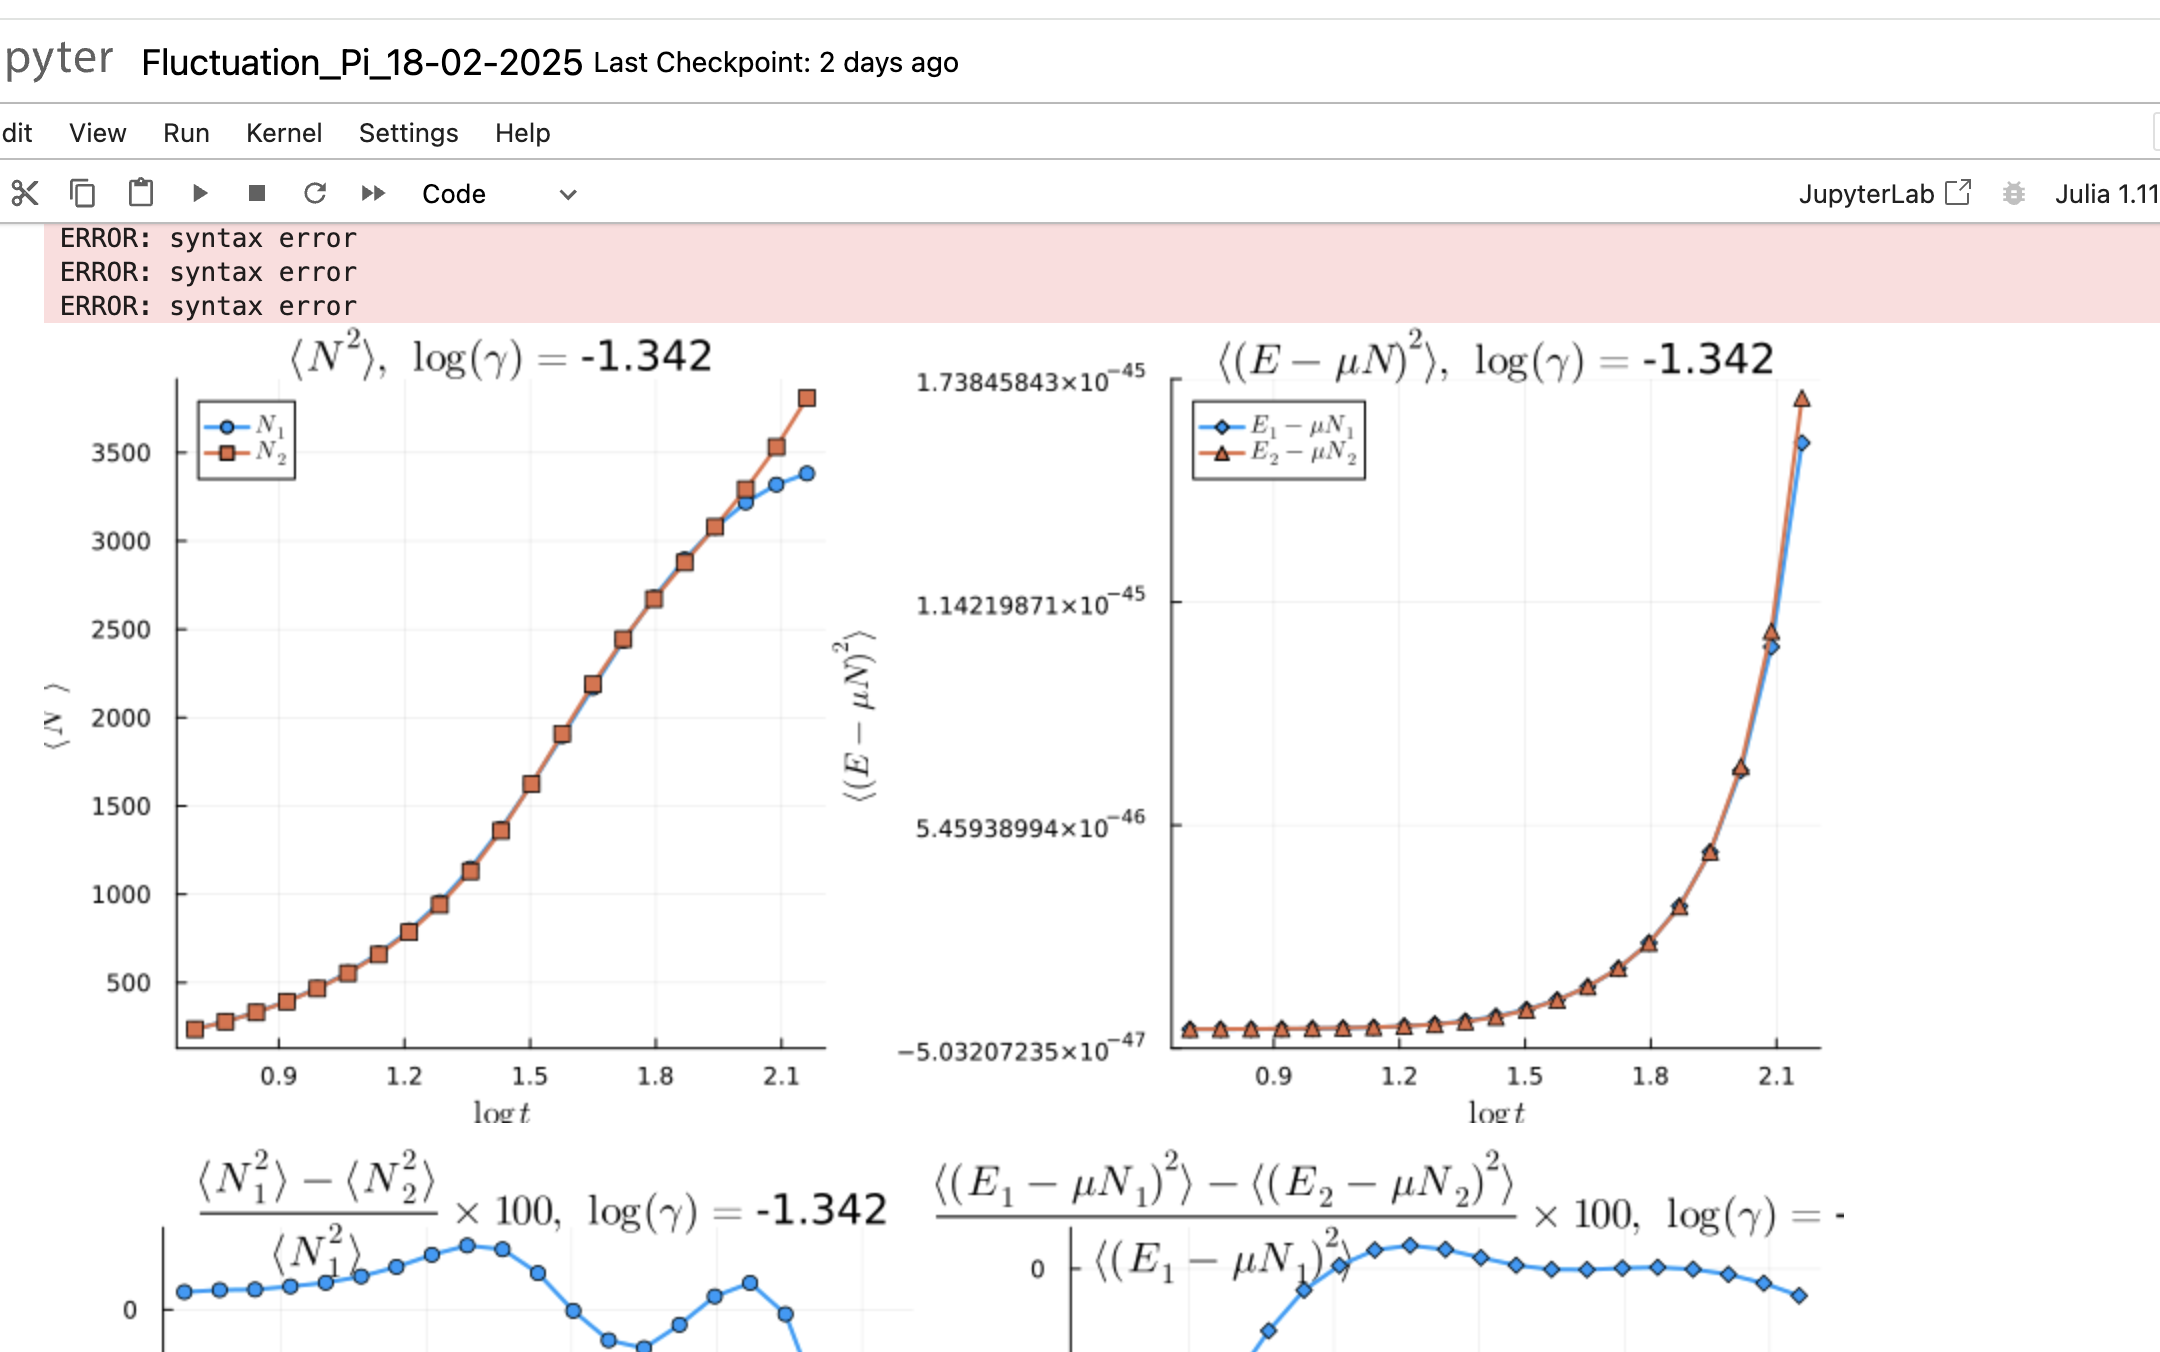
\includegraphics[width=1\textwidth]{Figures/test}

%\begin{aff}
%Donc une a l'ordre un en $\delta \theta (\operator{A}^{(0)})^{-1} %\operator{V}$ 

%\begin{eqnarray*}
%	\langle \delta \Pi ( \theta) \delta \Pi ( \theta') \rangle & = &  ( (\Pi^c_s - \Pi^c)\Pi^c/\Pi^c_s ) ( \theta ) \delta_{\theta, \theta'}/\delta \theta + \mathscr{F}(\theta , \theta' ) ,	
%\end{eqnarray*}

%avec 

%\begin{eqnarray*}
%	\mathscr{F}(\theta , \theta' ) & = & \left [ (\Pi^c_s - \Pi^c )( \theta)  +  (\Pi^c_s - \Pi^c ) ( \theta' )\right ] \frac{\Pi^c}{\Pi^c_s}(\theta)\frac{\Pi^c}{\Pi^c_s}(\theta') \frac{ \Delta( \theta'- \theta )}{ 2 \pi }\\
%	&&  - \left [ (\Pi^c_s - \Pi^c )( \theta)   (\Pi^c_s - \Pi^c ) ( \theta' )\right ] \frac{\Pi^c}{\Pi^c_s}(\theta)\frac{\Pi^c}{\Pi^c_s}(\theta')\int d\theta'' \left (   \frac{ \Pi^c/\Pi^c_s}{\Pi^c_s - \Pi^c} \right )(\theta'') \frac{\Delta(\theta''- \theta)}{2 \pi}\frac{\Delta(\theta''- \theta')}{2 \pi}  	
%\end{eqnarray*}
%\end{aff}



 









\subsection{Hamiltonien du modèle}
%Dans ce chapitre, nous nous intéressons aux fluctuations de la distribution de rapidité \( \delta \rho \) autour d'une distribution de référence \( \rho^c \), qui maximise la contribution à la fonction de partition des états, exprimée comme une fonctionnelle de la distribution \( \rho \) : 

La fonction de partition des états, s'exprime comme une fonctionnelle de la distribution \( \rho \) : 

\begin{eqnarray*}
	\Xi & = & \sum_\rho \exp \left( -\mathcal{A}(\rho) \right).
\end{eqnarray*}  

Dans la section {\em \bf Entropie de Yang-Yang} (\ref{??}), l'action \( \mathcal{A}(\rho) \) s'écrit sous la forme :  

\begin{eqnarray*}
	\mathcal{A}(\rho) & \doteq & - L\mathcal{S}_{YY}(\rho) + L\int f(\theta) \rho (\theta) \, d\theta,		
\end{eqnarray*}  

où \( \mathcal{S}_{YY} \) est la fonctionnelle d'entropie de Yang-Yang, définie dans (\ref{??}), et \( f \) est la fonction paramétrant les charges, introduite dans (\ref{??}).  

Dans cette même section {\em \bf Entropie de Yang-Yang} (\ref{??}), nous avons établi un lien entre \( f \) et distribution de référence \( \rho^c \), qui maximise la contribution à la fonction de partition des états .\\

On veux tester si nos experience est décrit pas un GGE. Pour cela nous nous intéressons aux fluctuations de la distribution de rapidité \( \delta \rho \) autour \( \rho^c \).

%Nous poursuivons à présent avec cette définition de l'action de classe $\mathcal{C}^2$ et admetant une distribution critique $\rho^c$ tel que sa différentielle en ce point critique soit nulle $d\mathcal{A}_{\rho^c} = 0 $ (\ref{??}) de sorte que d'aprés la formule de Taylor-Youg %afin de déterminer les fluctuations autour de \( \Pi^c \). Pour cela, nous réécrivons l'action sous la forme :  

Nous poursuivons à présent avec cette définition de l'action de classe $\mathcal{C}^2$ et admetant une distribution critique $\rho^c$ tel que sa différentielle en ce point critique soit nulle $d\mathcal{A}_{\rho^c} = 0 $ (\ref{??}) de sorte que d'aprés la formule de Taylor-Youg %afin de déterminer les fluctuations autour de \( \Pi^c \). Pour cela, nous réécrivons l'action sous la forme :  

\begin{eqnarray*}  
	\mathcal{A}(\rho^c + \delta \rho) & \underset{ \delta \rho \to 0 }{=} & \mathcal{A}(\rho^c)  + \frac{1}{2} \left. \frac{\delta^2 \mathcal{A}}{\delta \rho^2} \right|_{\rho^c} (\delta \rho) + \mathcal{O}((\delta \rho)^3),  
\end{eqnarray*}  

une expression quadratique pour l'action à l'ordre dominant en \( \delta \Pi \) avec $\left. \frac{\delta^2 \mathcal{A}}{\delta \rho^2} \right|_{\rho^c}$ la forme quadratique définie positive (Fig (\ref{fig.fluctu.A})).

\begin{figure}[H]
	\centering 
	\begin{tikzpicture}
		\begin{scope}[shift={(0,0)}]
			\begin{scope}[transform canvas={scale=0.6}]
				% Définition des couleurs avec les codes HTML
\definecolor{colorOne}{HTML}{443E46}
\definecolor{colorTwo}{HTML}{F6DEB8}
\definecolor{colorThree}{HTML}{908CA4}
\definecolor{colorFour}{HTML}{57659E}
\definecolor{colorFive}{HTML}{C57284}
\definecolor{colorSix}{HTML}{FF5B69}

% Raccourcis pour les couleurs
\def\colorOne{colorOne}
\def\colorTwo{colorTwo}
\def\colorThree{colorThree}
\def\colorFour{colorFour}
\def\colorFive{colorFive}
\def\colorSix{colorSix}

\def\colorslide{blue!50!black}



\begin{scope}
	% Tracer une courbe lisse entre des points
	\draw[shift={(0,0)} ,\colorOne]
		(-1 , 0 ) edge [thick,line width=0.8ex , ->,>=triangle 45  , \colorOne] node [pos = 1 , below ]{\huge$\rho$}( 5  , 0 )
	;
	\draw[shift={(0,0)}, color=\colorOne]
		(0, -1.0 ) edge [thick,line width=0.8ex , ->,>=triangle 45  ]node [pos=0.9,left=0.2cm ]{\huge$\mathcal{A}(\rho)$}( 0  , 5 )
	;
	\draw[]
		(2.5, 0.12 ) edge [thick,line width=0.8ex ,\colorThree ]node [pos=1,below  ]{\huge$\rho^c$} (2.5, -0.12 )	
	;
	
	\draw[]
		(2.5, -0.12 ) edge [thick,line width=0.4ex , dashed, \colorThree ] (2.5, 5.5 )
		(1.5, 1 ) edge [thick,line width=0.4ex , <->,>=triangle 45  , \colorThree ] (3.5, 1 )
		(-0.3,1) edge [thick,line width=0.4ex  , \colorThree ] node [pos=0,left ]{\huge$\mathcal{A}(\rho^c)$} (0.3, 1 )	
	;
    \draw[thick, line width=0.8ex , \colorFour] plot[smooth, tension=0.7] coordinates {
        (1, 5) (1.6 , 3 ) (2.5, 1) (3.5 , 3 )  (4, 5)
    };		
	
\end{scope}

	
			
			\end{scope}
			
			\draw[color = red , scale = 0.5 , draw = none  ] (-2 , -1) rectangle (5, 6) ; 	
		\end{scope}
		
		\begin{scope}[shift={(19,-1)}]
			\begin{scope}[transform canvas={scale=0.6}]
				% Définition des couleurs avec les codes HTML
\definecolor{colorOne}{HTML}{443E46}
\definecolor{colorTwo}{HTML}{F6DEB8}
\definecolor{colorThree}{HTML}{908CA4}
\definecolor{colorFour}{HTML}{57659E}
\definecolor{colorFive}{HTML}{C57284}
\definecolor{colorSix}{HTML}{FF5B69}

% Raccourcis pour les couleurs
\def\colorOne{colorOne}
\def\colorTwo{colorTwo}
\def\colorThree{colorThree}
\def\colorFour{colorFour}
\def\colorFive{colorFive}
\def\colorSix{colorSix}

\def\colorslide{blue!50!black}

\def\Occupation{
	\def\traitx{0.3}
	\def\traity{0.5}
	\draw[shift={(0,0)}]
		(-13.5 , 0 ) edge [thick,line width=0.8ex ]( -3.2  , 0 )
		( -3.2 - \traitx  , 0 - \traity ) edge [thick,line width=0.8ex ]( -3.2 + \traitx  , 0 + \traity  )
		( -2.8 - \traitx  , 0 - \traity ) edge [thick,line width=0.8ex ]( -2.8 + \traitx  , 0 + \traity  )
		(-2.8 , 0 ) edge [thick,line width=0.8ex ](2.8  , 0 )
		( 2.8 - \traitx  , 0 - \traity ) edge [thick,line width=0.8ex ]( 2.8 + \traitx  , 0 + \traity  )
		( 3.2 - \traitx  , 0 - \traity ) edge [thick,line width=0.8ex ]( 3.2 + \traitx  , 0 + \traity  )
		(3.2, 0 ) edge [thick,line width=0.8ex,->,>=triangle 45 , color = black ]node [pos=1.01,below  ]{\huge$\theta$}	( 13  , 0 )
	;
	\draw[shift={(0,0)}, color=\colorOne]
		(-10.5 , -1.5 ) edge [thick,line width=0.8ex , ->,>=triangle 45  ]( -10.5  , 4.5 )
	;
		
	\foreach \r in {1 , ... , 3 } {
%		\draw[
%		decoration={
%		markings,
%    	mark connection node=my node,
%    	mark=at position 0 with{\node [blue,transform shape] (my node) {\large \r};}},
%		color=gray, thick, 
%		line width=0.5ex] decorate { 
%            (-11.0, \r) -- (-10.1, \r )}
%        ;
        \draw[
			color=\colorOne,
			] 
            (-11.0, \r) edge[color=\colorThree , thick,line width=0.5ex] node [pos=-0.5 ]{\large\color{\colorFour} $\frac{\r}{\delta \theta}$ } (-10.3, \r )
        	;
	
	}
	

	
	% Graduation abcsisse 
	% Définitions des listes
% Definitions of the lists
\def\listetuple{-9/\theta_{1}, -8/\theta_{2} , -5/\theta_{3} , -2/\theta_{a-1} , 0/\theta_{a} , 1/\theta_{a+1} , 2/\theta_{a+2} ,  5/\theta_{N-4} , 7/\theta_{N-3},8/\theta_{N-1},9/\theta_{N} }
\def\listetrais{-12 , -11, -10, -9 , -8 , -7 ,  -6 , -5, -4.5,-4, -2 , -1, 0 , 0.5, 1, 2, 4 , 5 ,  6 , 7 , 8 ,8.5, 9 ,  10 , 11, 12 }

% Loop over listetrais
\foreach \r in \listetrais {
    % Initialize found variable to zero
    % Initialize found variable to zero
    %\pgfmathsetmacro\found{0}
    \global\def\found{0}
    \xdef\nomtheta{}
    
    % Check if \r is in listetuple
    \foreach \x/\y in \listetuple { 
        \ifdim \r pt=\x pt % If \r matches any \x in listetuple
            \global\def\found{1} ;
            \xdef\nomtheta{\y} % Set \nomtheta to the corresponding \y
            %\pgfmathsetmacro\found{1} % Set found to 1            
            %\global\pgfmathsetmacro\found{1}
        \fi
    }
    
    %\node [circle, draw, red] (A) at (\r, 2) {\found , $\nomtheta$};
    
    % Draw the line and display \nomtheta if found
    \ifnum\found=1
        \draw[color=\colorOne, thick, line width=0.5ex] 
            (\r, -0.3) -- (\r, 0.3) node[red , pos=-0.5] {\large $\nomtheta$};
         \filldraw[line width=0.5ex, color=\colorSix, outer color=\colorSix, inner color=\colorSix] 
            (\r, 0) circle (4pt);
    \else 
        % Draw without \nomtheta and add a blue circle if not found
        \draw[color=\colorOne, thick, line width=0.5ex] 
            (\r, -0.3) -- (\r, 0.3);
        \filldraw[line width=0.5ex, color=\colorSix, outer color=\colorTwo, inner color=\colorTwo] 
            (\r, 0) circle (4pt); 
    \fi
}

\def\listetrais{-9.5/\theta_{i-1}/2/3, -6.5/\theta_{i}/1/4  ,   -1.5/\theta_{j}/2/4 , 1.5/\theta_{j+1}/-1/3 , 3.5/\theta_{\ell-1}/1/3 , 6.5/\theta_{\ell}/3/4 , 9.5/\theta(\theta_{\ell+1})/-1/3 };



\foreach \r/\nomx/\y/\ys in \listetrais {
	\draw[
		decoration={
		markings,
    	mark connection node=my node,
    	mark=at position .5 with{\node [blue,transform shape] (my node) {\large \color{\colorFour} $\nomx$};}},
		color=\colorThree , thick, 
		line width=0.5ex] decorate { 
            (\r, 0.12) -- (\r, -1.2)}
        ;
     
     \ifdim \y pt > -1 pt 
     	\draw[
			decoration={
			markings,
    		mark connection node=my node,
    		mark=at position .5 with{\node [blue,transform shape] (my node) {\large \color{\colorFour} $\Pi(\nomx) $};}},
			color=\colorThree, thick, 
			line width=0.5ex] decorate { 
            (\r, \y) -- (\r +3, \y)}
        ;
        \draw[
			decoration={
			markings,
    		mark connection node=my node,
    		mark=at position .5 with{\node [blue,transform shape] (my node) {\large \color{\colorFive} $\Pi_s(\nomx) $};}},
			color=\colorFive, thick, 
			line width=0.5ex] decorate { 
            (\r, \ys) -- (\r +3, \ys)}
        ;
     \fi 
     \ifdim \r pt= -1.5 pt
     	\draw[
     		decoration={
			markings,
    		mark connection node=my node,
    		mark=at position .5 with{\node [blue,transform shape] (my node) {\large \color{\colorFour}  $\delta \theta $};},
    		%mark=at position 0.1  with {\arrow[blue, line width=0.5ex]{<}},
    		%mark=at position 1  with {\arrow[blue, line width=0.5ex]{>}}
    		},
        	color=\colorThree,
        	thick,
        	line width=0.5ex,
        	%arrows={Computer Modern Rightarrow[line cap=round]-Computer Modern Rightarrow[line cap=round]}
   			](\r, -1.2) edge[arrows={Computer Modern Rightarrow[line cap=round]-}] (\r + 0.4, -1.2)decorate {
    		(\r, -1.2) -- (\r + 3, -1.2)}(\r + 2, -1.2) edge[arrows={-Computer Modern Rightarrow[line cap=round]}] (\r + 3, -1.2)
    		;
    \fi
			
	
}


			
}


\begin{scope}
	%\draw[help lines , width=1.5ex] (-8,-3) grid (8,3);\draw[help lines ,width=0.5ex , opacity = 0.5] (-3,-3) grid[step=0.1] (3,3));
	
	%\draw[help lines] 
	%	(-3,-3) edge[width=1.5ex] grid (3,3)	
	%	(-3,-3) edge[width=0.5ex , opacity = 0.5] grid (3,3)	
	%;
	\begin{scope}[shift={(0,1)},rotate=0,opacity=1,color=black]
		\Occupation	
		
		%\node[anchor=east, font=\bfseries] at (-11, 0) {\color{red}\large (T = 0 )} ;	
	\end{scope}
	
	
	
	
	\begin{scope}[shift={(-10.5,7)},rotate=0,opacity=1,color=black]
	
	\begin{scope}[shift={(-0,0)},rotate=0,opacity=1,color=black]
	
		\draw[shift={(0,0)} ,line width=1ex,rounded corners = 1ex,color=\colorOne , opacity =1 ,fill=\colorOne!00 , pattern={north east lines} , pattern color=\colorOne!00 ]
			(0 , -1 ) rectangle (5,1)
		;
		

		\begin{scope}[shift={(0.5,0.5)}]
			\draw[color=\colorOne, thick, line width=0.5ex] 
            (0, -0.3) -- (0, 0.3) ;
            \filldraw[line width=0.5ex, color=\colorSix, outer color=\colorSix, inner color=\colorSix] 
            (0, 0) circle (4pt);
            
            \node[anchor=west, font=\bfseries] at (0.2, 0) {\color{\colorSix}\large : quasi-particule};
		\end{scope}
		
		\begin{scope}[shift={(0.5,-0.5)}]
			\draw[color=\colorOne, thick, line width=0.5ex] 
            (0, -0.3) -- (0, 0.3) ;
            \filldraw[line width=0.5ex, color=\colorSix, outer color=\colorTwo, inner color=\colorTwo] 
            (0, 0) circle (4pt);
            
            \node[anchor=west, font=\bfseries] at (0.2, 0) {\color{\colorSix}\large : hole};
		\end{scope}

	\end{scope}
	
	\begin{scope}[shift={(6,0)},rotate=0,opacity=1,color=black]	
		
		\draw[shift={(0,0)} ,line width=1ex,rounded corners = 1ex,color=\colorOne , opacity =1 ,fill=\colorOne!00 , pattern={north east lines} , pattern color=\colorOne!00 ]
			(0 , -1 ) rectangle (7.5,1)
		;
		
		\node[anchor=west] at (0.5, 0.5) {\color{\colorFour}\large $\Pi$ };\node[anchor=west, font=\bfseries] at (1, 0.5) {\color{\colorFour}\large : quasi-particule distribution};
		
		\node[anchor=west] at (0.5, -0.5) {\color{\colorFour}\large $\Pi_h$ };\node[anchor=west, font=\bfseries] at (1, -0.5) {\color{\colorFour}\large  : hole distribution};
		
	\end{scope}
	
	\begin{scope}[shift={(14.5,0)},rotate=0,opacity=1,color=black]	
		
		\draw[shift={(0,0)} ,line width=1ex,rounded corners = 1ex,color=\colorOne , opacity =1 ,fill=\colorOne!00 , pattern={north east lines} , pattern color=\colorOne!00 ]
			(0 , -0.5 ) rectangle (7.0,0.5)
		;
		
		\node[anchor=west] at (0.2, 0) {\color{\colorFour}\large ${\color{\colorFive}\Pi_s} = \Pi + \Pi_h $ } node[anchor=west , font=\bfseries] at (3.1 , 0 )  {\color{\colorFour}\large {\color{\colorFive} : density of states}};
		
	\end{scope}
	
	
	\end{scope}


		
	
\end{scope}

	
			
			\end{scope}
			\begin{scope}[scale=1]
				\draw[color = red , scale = 1 , draw = none  ] (-1 , -1) rectangle (5, 5) ; 
			\end{scope}	
		\end{scope}

		
				
			
	\end{tikzpicture}	
	\captionsetup{skip=10pt} % Ajoute de l’espace après la légende
	\label{fig.fluctu.A}
\end{figure}


On discrétise l'axe des rapidités en  petite cellule de rapidité $[\theta, \theta+\delta\theta]$, qui contient $L\rho(\theta) \delta \theta$ rapidités. 
	



Avec ces petites tranches, la forme quadratique s’écrit :

\begin{eqnarray*}
    \left. \frac{\delta^2 \mathcal{A}}{{\delta \rho}^2} \right|_{\rho^c}(\delta \rho ) &=&  \sum_{a,b \mid \text{tranche}}  
    \delta \rho(\theta_a)  \frac{\partial^2 \mathcal{A}}{\partial \delta \rho(\theta_a) \partial \delta \rho(\theta_b) } (\rho^c)  \delta \rho(\theta_b).
\end{eqnarray*}
Les fluctuations s’écrivent donc :

\begin{eqnarray*}
    \langle \delta \rho ( \theta) \delta \rho ( \theta') \rangle &=&  
    \frac{ \int d\delta \rho \, \delta \rho(\theta) \delta \rho ( \theta') 
    \exp \left( - \frac{1}{2} \sum_{a,b \mid \text{tranche}}  
    \delta \rho(\theta_a) \frac{\partial^2 \mathcal{A}}{\partial \delta \rho(\theta_a) \partial \delta \rho(\theta_b) } (\rho^c)  \delta \rho(\theta_b) \right) }
    { \int d\delta \Pi  
    \exp \left( - \frac{1}{2} \sum_{a,b \mid \text{tranche}}  
    \delta \rho(\theta_a) \frac{\partial^2 \mathcal{A}}{\partial \delta \rho(\theta_a) \partial \delta \rho(\theta_b) } (\rho^c)  \delta \rho(\theta_b) \right) } \\
    &=& \left( \mathbf{A}^{-1} \right)_{\theta , \theta'}
\end{eqnarray*}


\begin{aff}

\begin{eqnarray*}
	\langle \delta \rho ( \theta) \delta \rho ( \theta') \rangle &=& 	\left( \mathbf{A}^{-1} \right)_{\theta , \theta'}
\end{eqnarray*}

	
avec la  {\em matrice hessienne} $\mathbf{A}_{\theta , \theta'} \equiv \frac{\partial^2 \mathcal{A}}{\partial \delta \rho(\theta) \partial \delta \rho(\theta') }(\rho^c)$, au point critique/ qui maximise la probabilité  $\rho^c=\rho^c_s \nu^c $, s'écrit

\begin{eqnarray*}
	\operator{A} & = & \operator{A}^{(0)} + \delta \theta \operator{V}
\end{eqnarray*}

avec 

\begin{eqnarray*}
	A^{(0)}_{\theta , \theta'}  & = &  L\delta \theta \left ( \frac{ 1}{\rho^c_s ( 1  - \nu^c ) \nu^c } \right )(\theta)    \delta({\theta - \theta '})	,\\
	V_{\theta , \theta'}  &= & L \delta \theta \left \{ - \left [ \left ( \frac{1}{\rho^c_s( 1 - \nu^c) } \right ) ( \theta)  +  \left ( \frac{1}{\rho^c_s( 1 - \nu^c) } \right ) ( \theta' )\right ] \frac{ \Delta( \theta'- \theta )}{ 2 \pi } + \int d\theta''  \left ( \frac{\nu^c}{\rho^c_s( 1 - \nu^c) } \right )(\theta'') \frac{\Delta(\theta''- \theta)}{2 \pi}\frac{\Delta(\theta''- \theta')}{2 \pi}   \right \} 	
\end{eqnarray*}

\end{aff}

\subsection{Testes}

\begin{eqnarray*}
	\Delta_{\operator{\mathcal{N}}}^2  & = &  \frac{1}{\beta} \left . \frac{\partial \langle \operator{\mathcal{N}} \rangle}{\partial \mu} \right )_T \\
	\Delta_{\operator{\mathcal{E}}-\mu \operator{\mathcal{N}}}^2  & = &  - \left . \frac{\partial \langle \operator{\mathcal{E}}-\mu \operator{\mathcal{N}} \rangle}{\partial \beta} \right )_\mu 
\end{eqnarray*}

et 

\begin{eqnarray*}
	\Delta_{\operator{\mathcal{N}}}^2  &= & L^2 \int d\theta_a \int d \theta_b \, \langle \delta \rho(\theta_a) \delta \rho(\theta_b) \rangle \\
	\Delta_{\operator{\mathcal{E}}-\mu \operator{\mathcal{N}}}^2  & = & L^2 \int d\theta_a \int d \theta_b \, \left ( - \mu + \frac{1}2 m \theta_a^2  \right  )\left ( - \mu + \frac{1}2 m \theta_b^2  \right  )  \langle \delta \rho(\theta_a) \delta \rho(\theta_b) \rangle
\end{eqnarray*}

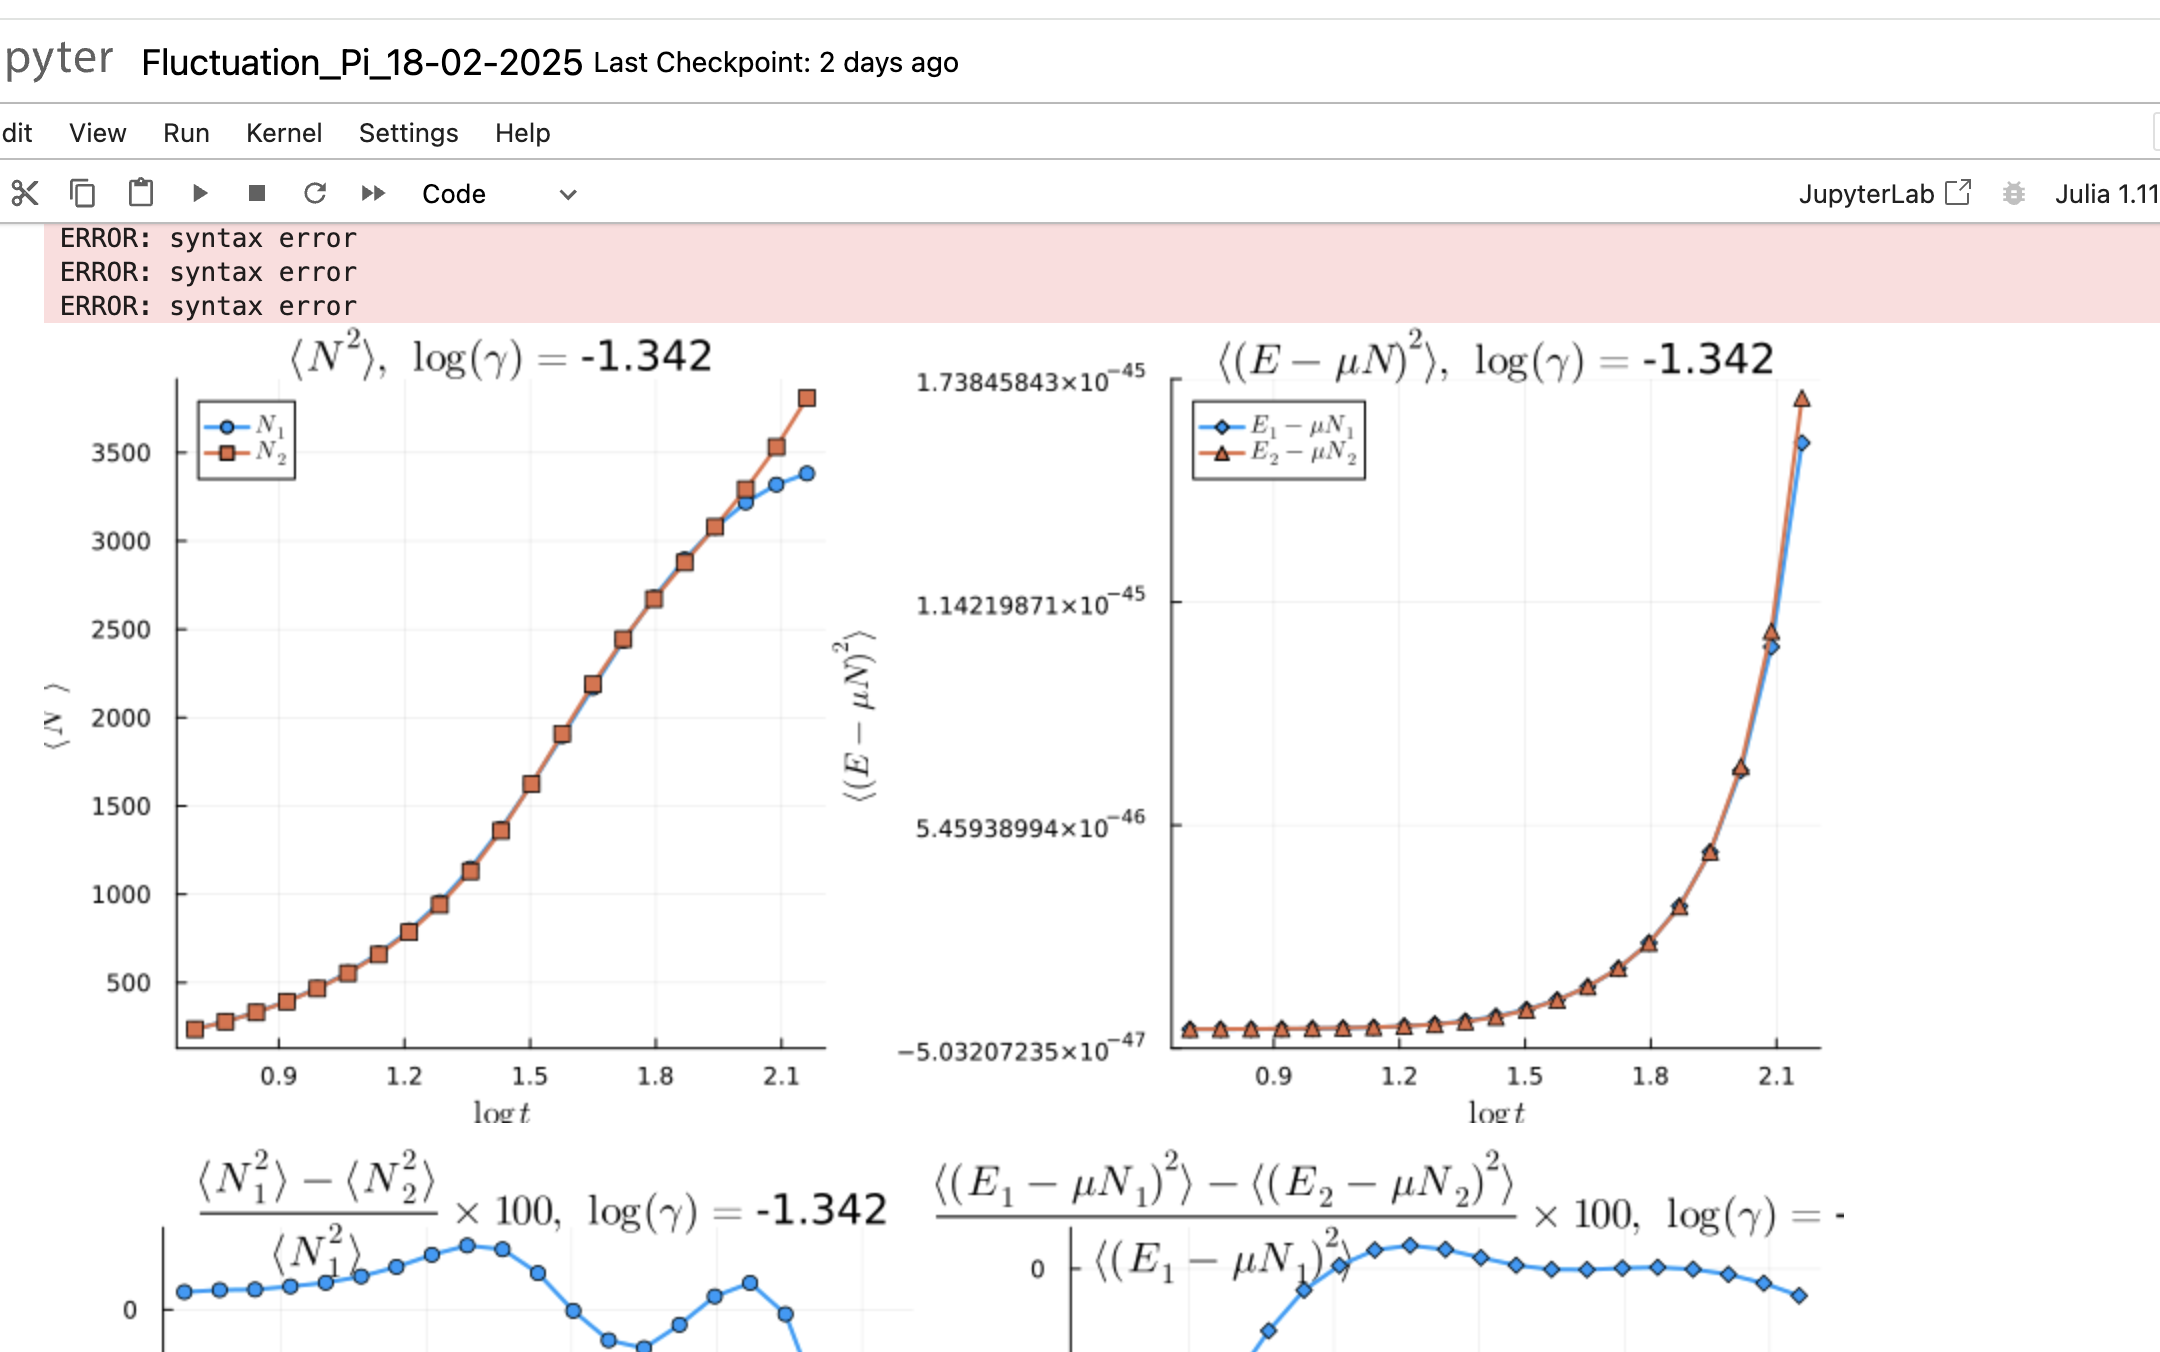
\includegraphics[width=1\textwidth]{Figures/test}

%\begin{aff}
%Donc une a l'ordre un en $\delta \theta (\operator{A}^{(0)})^{-1} %\operator{V}$ 

%\begin{eqnarray*}
%	\langle \delta \Pi ( \theta) \delta \Pi ( \theta') \rangle & = &  ( (\Pi^c_s - \Pi^c)\Pi^c/\Pi^c_s ) ( \theta ) \delta_{\theta, \theta'}/\delta \theta + \mathscr{F}(\theta , \theta' ) ,	
%\end{eqnarray*}

%avec 

%\begin{eqnarray*}
%	\mathscr{F}(\theta , \theta' ) & = & \left [ (\Pi^c_s - \Pi^c )( \theta)  +  (\Pi^c_s - \Pi^c ) ( \theta' )\right ] \frac{\Pi^c}{\Pi^c_s}(\theta)\frac{\Pi^c}{\Pi^c_s}(\theta') \frac{ \Delta( \theta'- \theta )}{ 2 \pi }\\
%	&&  - \left [ (\Pi^c_s - \Pi^c )( \theta)   (\Pi^c_s - \Pi^c ) ( \theta' )\right ] \frac{\Pi^c}{\Pi^c_s}(\theta)\frac{\Pi^c}{\Pi^c_s}(\theta')\int d\theta'' \left (   \frac{ \Pi^c/\Pi^c_s}{\Pi^c_s - \Pi^c} \right )(\theta'') \frac{\Delta(\theta''- \theta)}{2 \pi}\frac{\Delta(\theta''- \theta')}{2 \pi}  	
%\end{eqnarray*}
%\end{aff}



 









\subsection{États du vide et pseudovacuum}
%Dans ce chapitre, nous nous intéressons aux fluctuations de la distribution de rapidité \( \delta \rho \) autour d'une distribution de référence \( \rho^c \), qui maximise la contribution à la fonction de partition des états, exprimée comme une fonctionnelle de la distribution \( \rho \) : 

La fonction de partition des états, s'exprime comme une fonctionnelle de la distribution \( \rho \) : 

\begin{eqnarray*}
	\Xi & = & \sum_\rho \exp \left( -\mathcal{A}(\rho) \right).
\end{eqnarray*}  

Dans la section {\em \bf Entropie de Yang-Yang} (\ref{??}), l'action \( \mathcal{A}(\rho) \) s'écrit sous la forme :  

\begin{eqnarray*}
	\mathcal{A}(\rho) & \doteq & - L\mathcal{S}_{YY}(\rho) + L\int f(\theta) \rho (\theta) \, d\theta,		
\end{eqnarray*}  

où \( \mathcal{S}_{YY} \) est la fonctionnelle d'entropie de Yang-Yang, définie dans (\ref{??}), et \( f \) est la fonction paramétrant les charges, introduite dans (\ref{??}).  

Dans cette même section {\em \bf Entropie de Yang-Yang} (\ref{??}), nous avons établi un lien entre \( f \) et distribution de référence \( \rho^c \), qui maximise la contribution à la fonction de partition des états .\\

On veux tester si nos experience est décrit pas un GGE. Pour cela nous nous intéressons aux fluctuations de la distribution de rapidité \( \delta \rho \) autour \( \rho^c \).

%Nous poursuivons à présent avec cette définition de l'action de classe $\mathcal{C}^2$ et admetant une distribution critique $\rho^c$ tel que sa différentielle en ce point critique soit nulle $d\mathcal{A}_{\rho^c} = 0 $ (\ref{??}) de sorte que d'aprés la formule de Taylor-Youg %afin de déterminer les fluctuations autour de \( \Pi^c \). Pour cela, nous réécrivons l'action sous la forme :  

Nous poursuivons à présent avec cette définition de l'action de classe $\mathcal{C}^2$ et admetant une distribution critique $\rho^c$ tel que sa différentielle en ce point critique soit nulle $d\mathcal{A}_{\rho^c} = 0 $ (\ref{??}) de sorte que d'aprés la formule de Taylor-Youg %afin de déterminer les fluctuations autour de \( \Pi^c \). Pour cela, nous réécrivons l'action sous la forme :  

\begin{eqnarray*}  
	\mathcal{A}(\rho^c + \delta \rho) & \underset{ \delta \rho \to 0 }{=} & \mathcal{A}(\rho^c)  + \frac{1}{2} \left. \frac{\delta^2 \mathcal{A}}{\delta \rho^2} \right|_{\rho^c} (\delta \rho) + \mathcal{O}((\delta \rho)^3),  
\end{eqnarray*}  

une expression quadratique pour l'action à l'ordre dominant en \( \delta \Pi \) avec $\left. \frac{\delta^2 \mathcal{A}}{\delta \rho^2} \right|_{\rho^c}$ la forme quadratique définie positive (Fig (\ref{fig.fluctu.A})).

\begin{figure}[H]
	\centering 
	\begin{tikzpicture}
		\begin{scope}[shift={(0,0)}]
			\begin{scope}[transform canvas={scale=0.6}]
				% Définition des couleurs avec les codes HTML
\definecolor{colorOne}{HTML}{443E46}
\definecolor{colorTwo}{HTML}{F6DEB8}
\definecolor{colorThree}{HTML}{908CA4}
\definecolor{colorFour}{HTML}{57659E}
\definecolor{colorFive}{HTML}{C57284}
\definecolor{colorSix}{HTML}{FF5B69}

% Raccourcis pour les couleurs
\def\colorOne{colorOne}
\def\colorTwo{colorTwo}
\def\colorThree{colorThree}
\def\colorFour{colorFour}
\def\colorFive{colorFive}
\def\colorSix{colorSix}

\def\colorslide{blue!50!black}



\begin{scope}
	% Tracer une courbe lisse entre des points
	\draw[shift={(0,0)} ,\colorOne]
		(-1 , 0 ) edge [thick,line width=0.8ex , ->,>=triangle 45  , \colorOne] node [pos = 1 , below ]{\huge$\rho$}( 5  , 0 )
	;
	\draw[shift={(0,0)}, color=\colorOne]
		(0, -1.0 ) edge [thick,line width=0.8ex , ->,>=triangle 45  ]node [pos=0.9,left=0.2cm ]{\huge$\mathcal{A}(\rho)$}( 0  , 5 )
	;
	\draw[]
		(2.5, 0.12 ) edge [thick,line width=0.8ex ,\colorThree ]node [pos=1,below  ]{\huge$\rho^c$} (2.5, -0.12 )	
	;
	
	\draw[]
		(2.5, -0.12 ) edge [thick,line width=0.4ex , dashed, \colorThree ] (2.5, 5.5 )
		(1.5, 1 ) edge [thick,line width=0.4ex , <->,>=triangle 45  , \colorThree ] (3.5, 1 )
		(-0.3,1) edge [thick,line width=0.4ex  , \colorThree ] node [pos=0,left ]{\huge$\mathcal{A}(\rho^c)$} (0.3, 1 )	
	;
    \draw[thick, line width=0.8ex , \colorFour] plot[smooth, tension=0.7] coordinates {
        (1, 5) (1.6 , 3 ) (2.5, 1) (3.5 , 3 )  (4, 5)
    };		
	
\end{scope}

	
			
			\end{scope}
			
			\draw[color = red , scale = 0.5 , draw = none  ] (-2 , -1) rectangle (5, 6) ; 	
		\end{scope}
		
		\begin{scope}[shift={(19,-1)}]
			\begin{scope}[transform canvas={scale=0.6}]
				% Définition des couleurs avec les codes HTML
\definecolor{colorOne}{HTML}{443E46}
\definecolor{colorTwo}{HTML}{F6DEB8}
\definecolor{colorThree}{HTML}{908CA4}
\definecolor{colorFour}{HTML}{57659E}
\definecolor{colorFive}{HTML}{C57284}
\definecolor{colorSix}{HTML}{FF5B69}

% Raccourcis pour les couleurs
\def\colorOne{colorOne}
\def\colorTwo{colorTwo}
\def\colorThree{colorThree}
\def\colorFour{colorFour}
\def\colorFive{colorFive}
\def\colorSix{colorSix}

\def\colorslide{blue!50!black}

\def\Occupation{
	\def\traitx{0.3}
	\def\traity{0.5}
	\draw[shift={(0,0)}]
		(-13.5 , 0 ) edge [thick,line width=0.8ex ]( -3.2  , 0 )
		( -3.2 - \traitx  , 0 - \traity ) edge [thick,line width=0.8ex ]( -3.2 + \traitx  , 0 + \traity  )
		( -2.8 - \traitx  , 0 - \traity ) edge [thick,line width=0.8ex ]( -2.8 + \traitx  , 0 + \traity  )
		(-2.8 , 0 ) edge [thick,line width=0.8ex ](2.8  , 0 )
		( 2.8 - \traitx  , 0 - \traity ) edge [thick,line width=0.8ex ]( 2.8 + \traitx  , 0 + \traity  )
		( 3.2 - \traitx  , 0 - \traity ) edge [thick,line width=0.8ex ]( 3.2 + \traitx  , 0 + \traity  )
		(3.2, 0 ) edge [thick,line width=0.8ex,->,>=triangle 45 , color = black ]node [pos=1.01,below  ]{\huge$\theta$}	( 13  , 0 )
	;
	\draw[shift={(0,0)}, color=\colorOne]
		(-10.5 , -1.5 ) edge [thick,line width=0.8ex , ->,>=triangle 45  ]( -10.5  , 4.5 )
	;
		
	\foreach \r in {1 , ... , 3 } {
%		\draw[
%		decoration={
%		markings,
%    	mark connection node=my node,
%    	mark=at position 0 with{\node [blue,transform shape] (my node) {\large \r};}},
%		color=gray, thick, 
%		line width=0.5ex] decorate { 
%            (-11.0, \r) -- (-10.1, \r )}
%        ;
        \draw[
			color=\colorOne,
			] 
            (-11.0, \r) edge[color=\colorThree , thick,line width=0.5ex] node [pos=-0.5 ]{\large\color{\colorFour} $\frac{\r}{\delta \theta}$ } (-10.3, \r )
        	;
	
	}
	

	
	% Graduation abcsisse 
	% Définitions des listes
% Definitions of the lists
\def\listetuple{-9/\theta_{1}, -8/\theta_{2} , -5/\theta_{3} , -2/\theta_{a-1} , 0/\theta_{a} , 1/\theta_{a+1} , 2/\theta_{a+2} ,  5/\theta_{N-4} , 7/\theta_{N-3},8/\theta_{N-1},9/\theta_{N} }
\def\listetrais{-12 , -11, -10, -9 , -8 , -7 ,  -6 , -5, -4.5,-4, -2 , -1, 0 , 0.5, 1, 2, 4 , 5 ,  6 , 7 , 8 ,8.5, 9 ,  10 , 11, 12 }

% Loop over listetrais
\foreach \r in \listetrais {
    % Initialize found variable to zero
    % Initialize found variable to zero
    %\pgfmathsetmacro\found{0}
    \global\def\found{0}
    \xdef\nomtheta{}
    
    % Check if \r is in listetuple
    \foreach \x/\y in \listetuple { 
        \ifdim \r pt=\x pt % If \r matches any \x in listetuple
            \global\def\found{1} ;
            \xdef\nomtheta{\y} % Set \nomtheta to the corresponding \y
            %\pgfmathsetmacro\found{1} % Set found to 1            
            %\global\pgfmathsetmacro\found{1}
        \fi
    }
    
    %\node [circle, draw, red] (A) at (\r, 2) {\found , $\nomtheta$};
    
    % Draw the line and display \nomtheta if found
    \ifnum\found=1
        \draw[color=\colorOne, thick, line width=0.5ex] 
            (\r, -0.3) -- (\r, 0.3) node[red , pos=-0.5] {\large $\nomtheta$};
         \filldraw[line width=0.5ex, color=\colorSix, outer color=\colorSix, inner color=\colorSix] 
            (\r, 0) circle (4pt);
    \else 
        % Draw without \nomtheta and add a blue circle if not found
        \draw[color=\colorOne, thick, line width=0.5ex] 
            (\r, -0.3) -- (\r, 0.3);
        \filldraw[line width=0.5ex, color=\colorSix, outer color=\colorTwo, inner color=\colorTwo] 
            (\r, 0) circle (4pt); 
    \fi
}

\def\listetrais{-9.5/\theta_{i-1}/2/3, -6.5/\theta_{i}/1/4  ,   -1.5/\theta_{j}/2/4 , 1.5/\theta_{j+1}/-1/3 , 3.5/\theta_{\ell-1}/1/3 , 6.5/\theta_{\ell}/3/4 , 9.5/\theta(\theta_{\ell+1})/-1/3 };



\foreach \r/\nomx/\y/\ys in \listetrais {
	\draw[
		decoration={
		markings,
    	mark connection node=my node,
    	mark=at position .5 with{\node [blue,transform shape] (my node) {\large \color{\colorFour} $\nomx$};}},
		color=\colorThree , thick, 
		line width=0.5ex] decorate { 
            (\r, 0.12) -- (\r, -1.2)}
        ;
     
     \ifdim \y pt > -1 pt 
     	\draw[
			decoration={
			markings,
    		mark connection node=my node,
    		mark=at position .5 with{\node [blue,transform shape] (my node) {\large \color{\colorFour} $\Pi(\nomx) $};}},
			color=\colorThree, thick, 
			line width=0.5ex] decorate { 
            (\r, \y) -- (\r +3, \y)}
        ;
        \draw[
			decoration={
			markings,
    		mark connection node=my node,
    		mark=at position .5 with{\node [blue,transform shape] (my node) {\large \color{\colorFive} $\Pi_s(\nomx) $};}},
			color=\colorFive, thick, 
			line width=0.5ex] decorate { 
            (\r, \ys) -- (\r +3, \ys)}
        ;
     \fi 
     \ifdim \r pt= -1.5 pt
     	\draw[
     		decoration={
			markings,
    		mark connection node=my node,
    		mark=at position .5 with{\node [blue,transform shape] (my node) {\large \color{\colorFour}  $\delta \theta $};},
    		%mark=at position 0.1  with {\arrow[blue, line width=0.5ex]{<}},
    		%mark=at position 1  with {\arrow[blue, line width=0.5ex]{>}}
    		},
        	color=\colorThree,
        	thick,
        	line width=0.5ex,
        	%arrows={Computer Modern Rightarrow[line cap=round]-Computer Modern Rightarrow[line cap=round]}
   			](\r, -1.2) edge[arrows={Computer Modern Rightarrow[line cap=round]-}] (\r + 0.4, -1.2)decorate {
    		(\r, -1.2) -- (\r + 3, -1.2)}(\r + 2, -1.2) edge[arrows={-Computer Modern Rightarrow[line cap=round]}] (\r + 3, -1.2)
    		;
    \fi
			
	
}


			
}


\begin{scope}
	%\draw[help lines , width=1.5ex] (-8,-3) grid (8,3);\draw[help lines ,width=0.5ex , opacity = 0.5] (-3,-3) grid[step=0.1] (3,3));
	
	%\draw[help lines] 
	%	(-3,-3) edge[width=1.5ex] grid (3,3)	
	%	(-3,-3) edge[width=0.5ex , opacity = 0.5] grid (3,3)	
	%;
	\begin{scope}[shift={(0,1)},rotate=0,opacity=1,color=black]
		\Occupation	
		
		%\node[anchor=east, font=\bfseries] at (-11, 0) {\color{red}\large (T = 0 )} ;	
	\end{scope}
	
	
	
	
	\begin{scope}[shift={(-10.5,7)},rotate=0,opacity=1,color=black]
	
	\begin{scope}[shift={(-0,0)},rotate=0,opacity=1,color=black]
	
		\draw[shift={(0,0)} ,line width=1ex,rounded corners = 1ex,color=\colorOne , opacity =1 ,fill=\colorOne!00 , pattern={north east lines} , pattern color=\colorOne!00 ]
			(0 , -1 ) rectangle (5,1)
		;
		

		\begin{scope}[shift={(0.5,0.5)}]
			\draw[color=\colorOne, thick, line width=0.5ex] 
            (0, -0.3) -- (0, 0.3) ;
            \filldraw[line width=0.5ex, color=\colorSix, outer color=\colorSix, inner color=\colorSix] 
            (0, 0) circle (4pt);
            
            \node[anchor=west, font=\bfseries] at (0.2, 0) {\color{\colorSix}\large : quasi-particule};
		\end{scope}
		
		\begin{scope}[shift={(0.5,-0.5)}]
			\draw[color=\colorOne, thick, line width=0.5ex] 
            (0, -0.3) -- (0, 0.3) ;
            \filldraw[line width=0.5ex, color=\colorSix, outer color=\colorTwo, inner color=\colorTwo] 
            (0, 0) circle (4pt);
            
            \node[anchor=west, font=\bfseries] at (0.2, 0) {\color{\colorSix}\large : hole};
		\end{scope}

	\end{scope}
	
	\begin{scope}[shift={(6,0)},rotate=0,opacity=1,color=black]	
		
		\draw[shift={(0,0)} ,line width=1ex,rounded corners = 1ex,color=\colorOne , opacity =1 ,fill=\colorOne!00 , pattern={north east lines} , pattern color=\colorOne!00 ]
			(0 , -1 ) rectangle (7.5,1)
		;
		
		\node[anchor=west] at (0.5, 0.5) {\color{\colorFour}\large $\Pi$ };\node[anchor=west, font=\bfseries] at (1, 0.5) {\color{\colorFour}\large : quasi-particule distribution};
		
		\node[anchor=west] at (0.5, -0.5) {\color{\colorFour}\large $\Pi_h$ };\node[anchor=west, font=\bfseries] at (1, -0.5) {\color{\colorFour}\large  : hole distribution};
		
	\end{scope}
	
	\begin{scope}[shift={(14.5,0)},rotate=0,opacity=1,color=black]	
		
		\draw[shift={(0,0)} ,line width=1ex,rounded corners = 1ex,color=\colorOne , opacity =1 ,fill=\colorOne!00 , pattern={north east lines} , pattern color=\colorOne!00 ]
			(0 , -0.5 ) rectangle (7.0,0.5)
		;
		
		\node[anchor=west] at (0.2, 0) {\color{\colorFour}\large ${\color{\colorFive}\Pi_s} = \Pi + \Pi_h $ } node[anchor=west , font=\bfseries] at (3.1 , 0 )  {\color{\colorFour}\large {\color{\colorFive} : density of states}};
		
	\end{scope}
	
	
	\end{scope}


		
	
\end{scope}

	
			
			\end{scope}
			\begin{scope}[scale=1]
				\draw[color = red , scale = 1 , draw = none  ] (-1 , -1) rectangle (5, 5) ; 
			\end{scope}	
		\end{scope}

		
				
			
	\end{tikzpicture}	
	\captionsetup{skip=10pt} % Ajoute de l’espace après la légende
	\label{fig.fluctu.A}
\end{figure}


On discrétise l'axe des rapidités en  petite cellule de rapidité $[\theta, \theta+\delta\theta]$, qui contient $L\rho(\theta) \delta \theta$ rapidités. 
	



Avec ces petites tranches, la forme quadratique s’écrit :

\begin{eqnarray*}
    \left. \frac{\delta^2 \mathcal{A}}{{\delta \rho}^2} \right|_{\rho^c}(\delta \rho ) &=&  \sum_{a,b \mid \text{tranche}}  
    \delta \rho(\theta_a)  \frac{\partial^2 \mathcal{A}}{\partial \delta \rho(\theta_a) \partial \delta \rho(\theta_b) } (\rho^c)  \delta \rho(\theta_b).
\end{eqnarray*}
Les fluctuations s’écrivent donc :

\begin{eqnarray*}
    \langle \delta \rho ( \theta) \delta \rho ( \theta') \rangle &=&  
    \frac{ \int d\delta \rho \, \delta \rho(\theta) \delta \rho ( \theta') 
    \exp \left( - \frac{1}{2} \sum_{a,b \mid \text{tranche}}  
    \delta \rho(\theta_a) \frac{\partial^2 \mathcal{A}}{\partial \delta \rho(\theta_a) \partial \delta \rho(\theta_b) } (\rho^c)  \delta \rho(\theta_b) \right) }
    { \int d\delta \Pi  
    \exp \left( - \frac{1}{2} \sum_{a,b \mid \text{tranche}}  
    \delta \rho(\theta_a) \frac{\partial^2 \mathcal{A}}{\partial \delta \rho(\theta_a) \partial \delta \rho(\theta_b) } (\rho^c)  \delta \rho(\theta_b) \right) } \\
    &=& \left( \mathbf{A}^{-1} \right)_{\theta , \theta'}
\end{eqnarray*}


\begin{aff}

\begin{eqnarray*}
	\langle \delta \rho ( \theta) \delta \rho ( \theta') \rangle &=& 	\left( \mathbf{A}^{-1} \right)_{\theta , \theta'}
\end{eqnarray*}

	
avec la  {\em matrice hessienne} $\mathbf{A}_{\theta , \theta'} \equiv \frac{\partial^2 \mathcal{A}}{\partial \delta \rho(\theta) \partial \delta \rho(\theta') }(\rho^c)$, au point critique/ qui maximise la probabilité  $\rho^c=\rho^c_s \nu^c $, s'écrit

\begin{eqnarray*}
	\operator{A} & = & \operator{A}^{(0)} + \delta \theta \operator{V}
\end{eqnarray*}

avec 

\begin{eqnarray*}
	A^{(0)}_{\theta , \theta'}  & = &  L\delta \theta \left ( \frac{ 1}{\rho^c_s ( 1  - \nu^c ) \nu^c } \right )(\theta)    \delta({\theta - \theta '})	,\\
	V_{\theta , \theta'}  &= & L \delta \theta \left \{ - \left [ \left ( \frac{1}{\rho^c_s( 1 - \nu^c) } \right ) ( \theta)  +  \left ( \frac{1}{\rho^c_s( 1 - \nu^c) } \right ) ( \theta' )\right ] \frac{ \Delta( \theta'- \theta )}{ 2 \pi } + \int d\theta''  \left ( \frac{\nu^c}{\rho^c_s( 1 - \nu^c) } \right )(\theta'') \frac{\Delta(\theta''- \theta)}{2 \pi}\frac{\Delta(\theta''- \theta')}{2 \pi}   \right \} 	
\end{eqnarray*}

\end{aff}

\subsection{Testes}

\begin{eqnarray*}
	\Delta_{\operator{\mathcal{N}}}^2  & = &  \frac{1}{\beta} \left . \frac{\partial \langle \operator{\mathcal{N}} \rangle}{\partial \mu} \right )_T \\
	\Delta_{\operator{\mathcal{E}}-\mu \operator{\mathcal{N}}}^2  & = &  - \left . \frac{\partial \langle \operator{\mathcal{E}}-\mu \operator{\mathcal{N}} \rangle}{\partial \beta} \right )_\mu 
\end{eqnarray*}

et 

\begin{eqnarray*}
	\Delta_{\operator{\mathcal{N}}}^2  &= & L^2 \int d\theta_a \int d \theta_b \, \langle \delta \rho(\theta_a) \delta \rho(\theta_b) \rangle \\
	\Delta_{\operator{\mathcal{E}}-\mu \operator{\mathcal{N}}}^2  & = & L^2 \int d\theta_a \int d \theta_b \, \left ( - \mu + \frac{1}2 m \theta_a^2  \right  )\left ( - \mu + \frac{1}2 m \theta_b^2  \right  )  \langle \delta \rho(\theta_a) \delta \rho(\theta_b) \rangle
\end{eqnarray*}

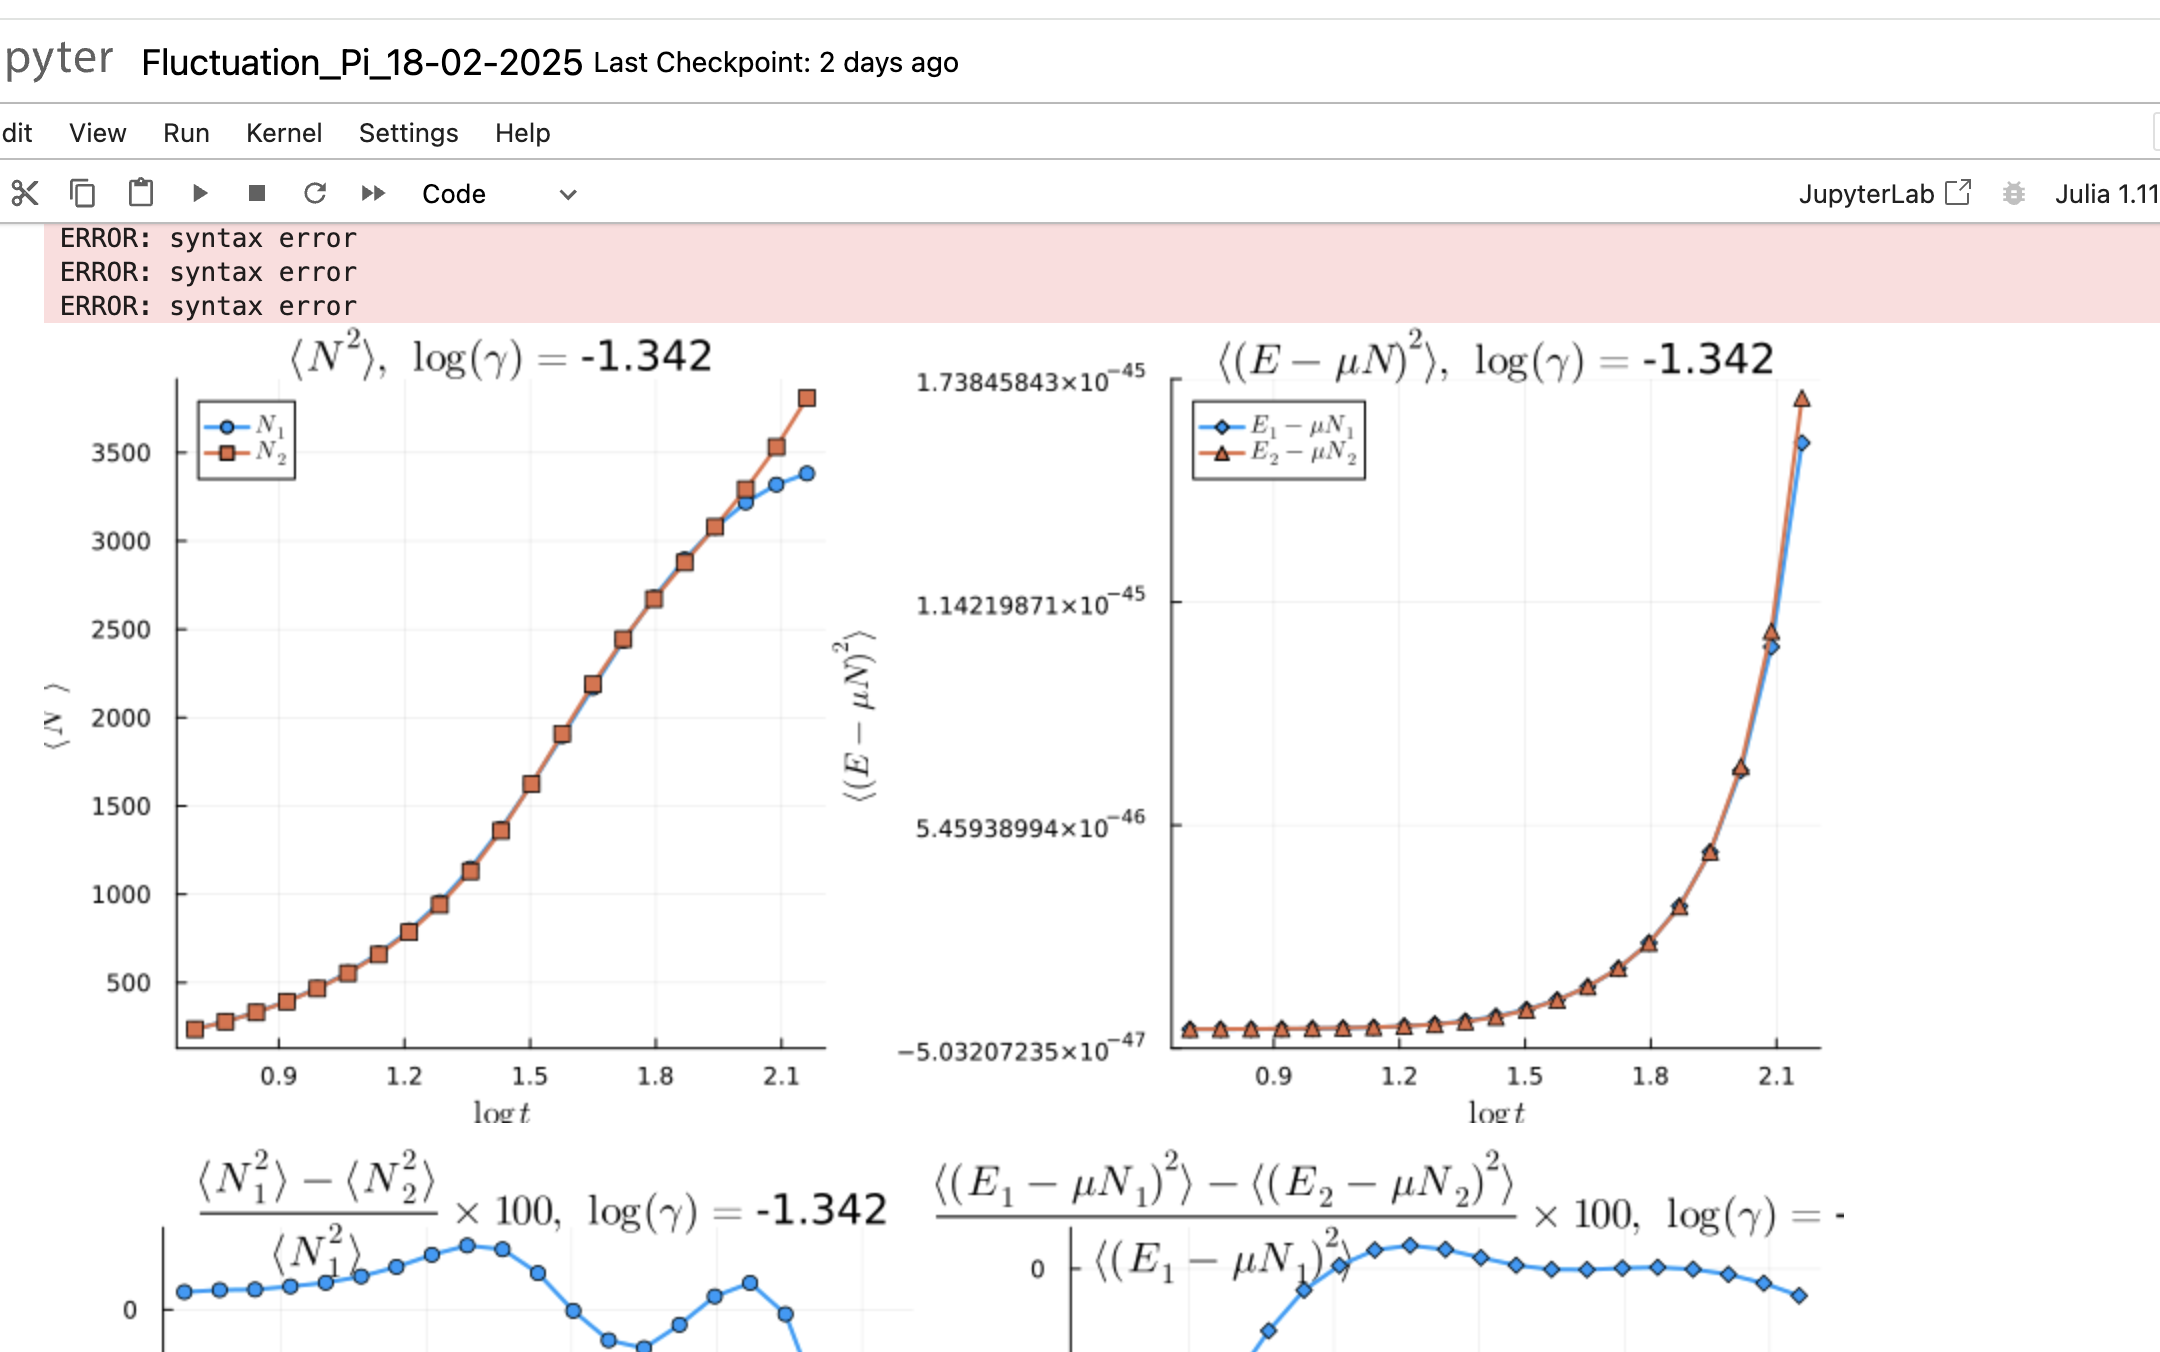
\includegraphics[width=1\textwidth]{Figures/test}

%\begin{aff}
%Donc une a l'ordre un en $\delta \theta (\operator{A}^{(0)})^{-1} %\operator{V}$ 

%\begin{eqnarray*}
%	\langle \delta \Pi ( \theta) \delta \Pi ( \theta') \rangle & = &  ( (\Pi^c_s - \Pi^c)\Pi^c/\Pi^c_s ) ( \theta ) \delta_{\theta, \theta'}/\delta \theta + \mathscr{F}(\theta , \theta' ) ,	
%\end{eqnarray*}

%avec 

%\begin{eqnarray*}
%	\mathscr{F}(\theta , \theta' ) & = & \left [ (\Pi^c_s - \Pi^c )( \theta)  +  (\Pi^c_s - \Pi^c ) ( \theta' )\right ] \frac{\Pi^c}{\Pi^c_s}(\theta)\frac{\Pi^c}{\Pi^c_s}(\theta') \frac{ \Delta( \theta'- \theta )}{ 2 \pi }\\
%	&&  - \left [ (\Pi^c_s - \Pi^c )( \theta)   (\Pi^c_s - \Pi^c ) ( \theta' )\right ] \frac{\Pi^c}{\Pi^c_s}(\theta)\frac{\Pi^c}{\Pi^c_s}(\theta')\int d\theta'' \left (   \frac{ \Pi^c/\Pi^c_s}{\Pi^c_s - \Pi^c} \right )(\theta'') \frac{\Delta(\theta''- \theta)}{2 \pi}\frac{\Delta(\theta''- \theta')}{2 \pi}  	
%\end{eqnarray*}
%\end{aff}



 










\subsection{Opérateurs conservés (intégrales du mouvement)}
%Dans ce chapitre, nous nous intéressons aux fluctuations de la distribution de rapidité \( \delta \rho \) autour d'une distribution de référence \( \rho^c \), qui maximise la contribution à la fonction de partition des états, exprimée comme une fonctionnelle de la distribution \( \rho \) : 

La fonction de partition des états, s'exprime comme une fonctionnelle de la distribution \( \rho \) : 

\begin{eqnarray*}
	\Xi & = & \sum_\rho \exp \left( -\mathcal{A}(\rho) \right).
\end{eqnarray*}  

Dans la section {\em \bf Entropie de Yang-Yang} (\ref{??}), l'action \( \mathcal{A}(\rho) \) s'écrit sous la forme :  

\begin{eqnarray*}
	\mathcal{A}(\rho) & \doteq & - L\mathcal{S}_{YY}(\rho) + L\int f(\theta) \rho (\theta) \, d\theta,		
\end{eqnarray*}  

où \( \mathcal{S}_{YY} \) est la fonctionnelle d'entropie de Yang-Yang, définie dans (\ref{??}), et \( f \) est la fonction paramétrant les charges, introduite dans (\ref{??}).  

Dans cette même section {\em \bf Entropie de Yang-Yang} (\ref{??}), nous avons établi un lien entre \( f \) et distribution de référence \( \rho^c \), qui maximise la contribution à la fonction de partition des états .\\

On veux tester si nos experience est décrit pas un GGE. Pour cela nous nous intéressons aux fluctuations de la distribution de rapidité \( \delta \rho \) autour \( \rho^c \).

%Nous poursuivons à présent avec cette définition de l'action de classe $\mathcal{C}^2$ et admetant une distribution critique $\rho^c$ tel que sa différentielle en ce point critique soit nulle $d\mathcal{A}_{\rho^c} = 0 $ (\ref{??}) de sorte que d'aprés la formule de Taylor-Youg %afin de déterminer les fluctuations autour de \( \Pi^c \). Pour cela, nous réécrivons l'action sous la forme :  

Nous poursuivons à présent avec cette définition de l'action de classe $\mathcal{C}^2$ et admetant une distribution critique $\rho^c$ tel que sa différentielle en ce point critique soit nulle $d\mathcal{A}_{\rho^c} = 0 $ (\ref{??}) de sorte que d'aprés la formule de Taylor-Youg %afin de déterminer les fluctuations autour de \( \Pi^c \). Pour cela, nous réécrivons l'action sous la forme :  

\begin{eqnarray*}  
	\mathcal{A}(\rho^c + \delta \rho) & \underset{ \delta \rho \to 0 }{=} & \mathcal{A}(\rho^c)  + \frac{1}{2} \left. \frac{\delta^2 \mathcal{A}}{\delta \rho^2} \right|_{\rho^c} (\delta \rho) + \mathcal{O}((\delta \rho)^3),  
\end{eqnarray*}  

une expression quadratique pour l'action à l'ordre dominant en \( \delta \Pi \) avec $\left. \frac{\delta^2 \mathcal{A}}{\delta \rho^2} \right|_{\rho^c}$ la forme quadratique définie positive (Fig (\ref{fig.fluctu.A})).

\begin{figure}[H]
	\centering 
	\begin{tikzpicture}
		\begin{scope}[shift={(0,0)}]
			\begin{scope}[transform canvas={scale=0.6}]
				% Définition des couleurs avec les codes HTML
\definecolor{colorOne}{HTML}{443E46}
\definecolor{colorTwo}{HTML}{F6DEB8}
\definecolor{colorThree}{HTML}{908CA4}
\definecolor{colorFour}{HTML}{57659E}
\definecolor{colorFive}{HTML}{C57284}
\definecolor{colorSix}{HTML}{FF5B69}

% Raccourcis pour les couleurs
\def\colorOne{colorOne}
\def\colorTwo{colorTwo}
\def\colorThree{colorThree}
\def\colorFour{colorFour}
\def\colorFive{colorFive}
\def\colorSix{colorSix}

\def\colorslide{blue!50!black}



\begin{scope}
	% Tracer une courbe lisse entre des points
	\draw[shift={(0,0)} ,\colorOne]
		(-1 , 0 ) edge [thick,line width=0.8ex , ->,>=triangle 45  , \colorOne] node [pos = 1 , below ]{\huge$\rho$}( 5  , 0 )
	;
	\draw[shift={(0,0)}, color=\colorOne]
		(0, -1.0 ) edge [thick,line width=0.8ex , ->,>=triangle 45  ]node [pos=0.9,left=0.2cm ]{\huge$\mathcal{A}(\rho)$}( 0  , 5 )
	;
	\draw[]
		(2.5, 0.12 ) edge [thick,line width=0.8ex ,\colorThree ]node [pos=1,below  ]{\huge$\rho^c$} (2.5, -0.12 )	
	;
	
	\draw[]
		(2.5, -0.12 ) edge [thick,line width=0.4ex , dashed, \colorThree ] (2.5, 5.5 )
		(1.5, 1 ) edge [thick,line width=0.4ex , <->,>=triangle 45  , \colorThree ] (3.5, 1 )
		(-0.3,1) edge [thick,line width=0.4ex  , \colorThree ] node [pos=0,left ]{\huge$\mathcal{A}(\rho^c)$} (0.3, 1 )	
	;
    \draw[thick, line width=0.8ex , \colorFour] plot[smooth, tension=0.7] coordinates {
        (1, 5) (1.6 , 3 ) (2.5, 1) (3.5 , 3 )  (4, 5)
    };		
	
\end{scope}

	
			
			\end{scope}
			
			\draw[color = red , scale = 0.5 , draw = none  ] (-2 , -1) rectangle (5, 6) ; 	
		\end{scope}
		
		\begin{scope}[shift={(19,-1)}]
			\begin{scope}[transform canvas={scale=0.6}]
				% Définition des couleurs avec les codes HTML
\definecolor{colorOne}{HTML}{443E46}
\definecolor{colorTwo}{HTML}{F6DEB8}
\definecolor{colorThree}{HTML}{908CA4}
\definecolor{colorFour}{HTML}{57659E}
\definecolor{colorFive}{HTML}{C57284}
\definecolor{colorSix}{HTML}{FF5B69}

% Raccourcis pour les couleurs
\def\colorOne{colorOne}
\def\colorTwo{colorTwo}
\def\colorThree{colorThree}
\def\colorFour{colorFour}
\def\colorFive{colorFive}
\def\colorSix{colorSix}

\def\colorslide{blue!50!black}

\def\Occupation{
	\def\traitx{0.3}
	\def\traity{0.5}
	\draw[shift={(0,0)}]
		(-13.5 , 0 ) edge [thick,line width=0.8ex ]( -3.2  , 0 )
		( -3.2 - \traitx  , 0 - \traity ) edge [thick,line width=0.8ex ]( -3.2 + \traitx  , 0 + \traity  )
		( -2.8 - \traitx  , 0 - \traity ) edge [thick,line width=0.8ex ]( -2.8 + \traitx  , 0 + \traity  )
		(-2.8 , 0 ) edge [thick,line width=0.8ex ](2.8  , 0 )
		( 2.8 - \traitx  , 0 - \traity ) edge [thick,line width=0.8ex ]( 2.8 + \traitx  , 0 + \traity  )
		( 3.2 - \traitx  , 0 - \traity ) edge [thick,line width=0.8ex ]( 3.2 + \traitx  , 0 + \traity  )
		(3.2, 0 ) edge [thick,line width=0.8ex,->,>=triangle 45 , color = black ]node [pos=1.01,below  ]{\huge$\theta$}	( 13  , 0 )
	;
	\draw[shift={(0,0)}, color=\colorOne]
		(-10.5 , -1.5 ) edge [thick,line width=0.8ex , ->,>=triangle 45  ]( -10.5  , 4.5 )
	;
		
	\foreach \r in {1 , ... , 3 } {
%		\draw[
%		decoration={
%		markings,
%    	mark connection node=my node,
%    	mark=at position 0 with{\node [blue,transform shape] (my node) {\large \r};}},
%		color=gray, thick, 
%		line width=0.5ex] decorate { 
%            (-11.0, \r) -- (-10.1, \r )}
%        ;
        \draw[
			color=\colorOne,
			] 
            (-11.0, \r) edge[color=\colorThree , thick,line width=0.5ex] node [pos=-0.5 ]{\large\color{\colorFour} $\frac{\r}{\delta \theta}$ } (-10.3, \r )
        	;
	
	}
	

	
	% Graduation abcsisse 
	% Définitions des listes
% Definitions of the lists
\def\listetuple{-9/\theta_{1}, -8/\theta_{2} , -5/\theta_{3} , -2/\theta_{a-1} , 0/\theta_{a} , 1/\theta_{a+1} , 2/\theta_{a+2} ,  5/\theta_{N-4} , 7/\theta_{N-3},8/\theta_{N-1},9/\theta_{N} }
\def\listetrais{-12 , -11, -10, -9 , -8 , -7 ,  -6 , -5, -4.5,-4, -2 , -1, 0 , 0.5, 1, 2, 4 , 5 ,  6 , 7 , 8 ,8.5, 9 ,  10 , 11, 12 }

% Loop over listetrais
\foreach \r in \listetrais {
    % Initialize found variable to zero
    % Initialize found variable to zero
    %\pgfmathsetmacro\found{0}
    \global\def\found{0}
    \xdef\nomtheta{}
    
    % Check if \r is in listetuple
    \foreach \x/\y in \listetuple { 
        \ifdim \r pt=\x pt % If \r matches any \x in listetuple
            \global\def\found{1} ;
            \xdef\nomtheta{\y} % Set \nomtheta to the corresponding \y
            %\pgfmathsetmacro\found{1} % Set found to 1            
            %\global\pgfmathsetmacro\found{1}
        \fi
    }
    
    %\node [circle, draw, red] (A) at (\r, 2) {\found , $\nomtheta$};
    
    % Draw the line and display \nomtheta if found
    \ifnum\found=1
        \draw[color=\colorOne, thick, line width=0.5ex] 
            (\r, -0.3) -- (\r, 0.3) node[red , pos=-0.5] {\large $\nomtheta$};
         \filldraw[line width=0.5ex, color=\colorSix, outer color=\colorSix, inner color=\colorSix] 
            (\r, 0) circle (4pt);
    \else 
        % Draw without \nomtheta and add a blue circle if not found
        \draw[color=\colorOne, thick, line width=0.5ex] 
            (\r, -0.3) -- (\r, 0.3);
        \filldraw[line width=0.5ex, color=\colorSix, outer color=\colorTwo, inner color=\colorTwo] 
            (\r, 0) circle (4pt); 
    \fi
}

\def\listetrais{-9.5/\theta_{i-1}/2/3, -6.5/\theta_{i}/1/4  ,   -1.5/\theta_{j}/2/4 , 1.5/\theta_{j+1}/-1/3 , 3.5/\theta_{\ell-1}/1/3 , 6.5/\theta_{\ell}/3/4 , 9.5/\theta(\theta_{\ell+1})/-1/3 };



\foreach \r/\nomx/\y/\ys in \listetrais {
	\draw[
		decoration={
		markings,
    	mark connection node=my node,
    	mark=at position .5 with{\node [blue,transform shape] (my node) {\large \color{\colorFour} $\nomx$};}},
		color=\colorThree , thick, 
		line width=0.5ex] decorate { 
            (\r, 0.12) -- (\r, -1.2)}
        ;
     
     \ifdim \y pt > -1 pt 
     	\draw[
			decoration={
			markings,
    		mark connection node=my node,
    		mark=at position .5 with{\node [blue,transform shape] (my node) {\large \color{\colorFour} $\Pi(\nomx) $};}},
			color=\colorThree, thick, 
			line width=0.5ex] decorate { 
            (\r, \y) -- (\r +3, \y)}
        ;
        \draw[
			decoration={
			markings,
    		mark connection node=my node,
    		mark=at position .5 with{\node [blue,transform shape] (my node) {\large \color{\colorFive} $\Pi_s(\nomx) $};}},
			color=\colorFive, thick, 
			line width=0.5ex] decorate { 
            (\r, \ys) -- (\r +3, \ys)}
        ;
     \fi 
     \ifdim \r pt= -1.5 pt
     	\draw[
     		decoration={
			markings,
    		mark connection node=my node,
    		mark=at position .5 with{\node [blue,transform shape] (my node) {\large \color{\colorFour}  $\delta \theta $};},
    		%mark=at position 0.1  with {\arrow[blue, line width=0.5ex]{<}},
    		%mark=at position 1  with {\arrow[blue, line width=0.5ex]{>}}
    		},
        	color=\colorThree,
        	thick,
        	line width=0.5ex,
        	%arrows={Computer Modern Rightarrow[line cap=round]-Computer Modern Rightarrow[line cap=round]}
   			](\r, -1.2) edge[arrows={Computer Modern Rightarrow[line cap=round]-}] (\r + 0.4, -1.2)decorate {
    		(\r, -1.2) -- (\r + 3, -1.2)}(\r + 2, -1.2) edge[arrows={-Computer Modern Rightarrow[line cap=round]}] (\r + 3, -1.2)
    		;
    \fi
			
	
}


			
}


\begin{scope}
	%\draw[help lines , width=1.5ex] (-8,-3) grid (8,3);\draw[help lines ,width=0.5ex , opacity = 0.5] (-3,-3) grid[step=0.1] (3,3));
	
	%\draw[help lines] 
	%	(-3,-3) edge[width=1.5ex] grid (3,3)	
	%	(-3,-3) edge[width=0.5ex , opacity = 0.5] grid (3,3)	
	%;
	\begin{scope}[shift={(0,1)},rotate=0,opacity=1,color=black]
		\Occupation	
		
		%\node[anchor=east, font=\bfseries] at (-11, 0) {\color{red}\large (T = 0 )} ;	
	\end{scope}
	
	
	
	
	\begin{scope}[shift={(-10.5,7)},rotate=0,opacity=1,color=black]
	
	\begin{scope}[shift={(-0,0)},rotate=0,opacity=1,color=black]
	
		\draw[shift={(0,0)} ,line width=1ex,rounded corners = 1ex,color=\colorOne , opacity =1 ,fill=\colorOne!00 , pattern={north east lines} , pattern color=\colorOne!00 ]
			(0 , -1 ) rectangle (5,1)
		;
		

		\begin{scope}[shift={(0.5,0.5)}]
			\draw[color=\colorOne, thick, line width=0.5ex] 
            (0, -0.3) -- (0, 0.3) ;
            \filldraw[line width=0.5ex, color=\colorSix, outer color=\colorSix, inner color=\colorSix] 
            (0, 0) circle (4pt);
            
            \node[anchor=west, font=\bfseries] at (0.2, 0) {\color{\colorSix}\large : quasi-particule};
		\end{scope}
		
		\begin{scope}[shift={(0.5,-0.5)}]
			\draw[color=\colorOne, thick, line width=0.5ex] 
            (0, -0.3) -- (0, 0.3) ;
            \filldraw[line width=0.5ex, color=\colorSix, outer color=\colorTwo, inner color=\colorTwo] 
            (0, 0) circle (4pt);
            
            \node[anchor=west, font=\bfseries] at (0.2, 0) {\color{\colorSix}\large : hole};
		\end{scope}

	\end{scope}
	
	\begin{scope}[shift={(6,0)},rotate=0,opacity=1,color=black]	
		
		\draw[shift={(0,0)} ,line width=1ex,rounded corners = 1ex,color=\colorOne , opacity =1 ,fill=\colorOne!00 , pattern={north east lines} , pattern color=\colorOne!00 ]
			(0 , -1 ) rectangle (7.5,1)
		;
		
		\node[anchor=west] at (0.5, 0.5) {\color{\colorFour}\large $\Pi$ };\node[anchor=west, font=\bfseries] at (1, 0.5) {\color{\colorFour}\large : quasi-particule distribution};
		
		\node[anchor=west] at (0.5, -0.5) {\color{\colorFour}\large $\Pi_h$ };\node[anchor=west, font=\bfseries] at (1, -0.5) {\color{\colorFour}\large  : hole distribution};
		
	\end{scope}
	
	\begin{scope}[shift={(14.5,0)},rotate=0,opacity=1,color=black]	
		
		\draw[shift={(0,0)} ,line width=1ex,rounded corners = 1ex,color=\colorOne , opacity =1 ,fill=\colorOne!00 , pattern={north east lines} , pattern color=\colorOne!00 ]
			(0 , -0.5 ) rectangle (7.0,0.5)
		;
		
		\node[anchor=west] at (0.2, 0) {\color{\colorFour}\large ${\color{\colorFive}\Pi_s} = \Pi + \Pi_h $ } node[anchor=west , font=\bfseries] at (3.1 , 0 )  {\color{\colorFour}\large {\color{\colorFive} : density of states}};
		
	\end{scope}
	
	
	\end{scope}


		
	
\end{scope}

	
			
			\end{scope}
			\begin{scope}[scale=1]
				\draw[color = red , scale = 1 , draw = none  ] (-1 , -1) rectangle (5, 5) ; 
			\end{scope}	
		\end{scope}

		
				
			
	\end{tikzpicture}	
	\captionsetup{skip=10pt} % Ajoute de l’espace après la légende
	\label{fig.fluctu.A}
\end{figure}


On discrétise l'axe des rapidités en  petite cellule de rapidité $[\theta, \theta+\delta\theta]$, qui contient $L\rho(\theta) \delta \theta$ rapidités. 
	



Avec ces petites tranches, la forme quadratique s’écrit :

\begin{eqnarray*}
    \left. \frac{\delta^2 \mathcal{A}}{{\delta \rho}^2} \right|_{\rho^c}(\delta \rho ) &=&  \sum_{a,b \mid \text{tranche}}  
    \delta \rho(\theta_a)  \frac{\partial^2 \mathcal{A}}{\partial \delta \rho(\theta_a) \partial \delta \rho(\theta_b) } (\rho^c)  \delta \rho(\theta_b).
\end{eqnarray*}
Les fluctuations s’écrivent donc :

\begin{eqnarray*}
    \langle \delta \rho ( \theta) \delta \rho ( \theta') \rangle &=&  
    \frac{ \int d\delta \rho \, \delta \rho(\theta) \delta \rho ( \theta') 
    \exp \left( - \frac{1}{2} \sum_{a,b \mid \text{tranche}}  
    \delta \rho(\theta_a) \frac{\partial^2 \mathcal{A}}{\partial \delta \rho(\theta_a) \partial \delta \rho(\theta_b) } (\rho^c)  \delta \rho(\theta_b) \right) }
    { \int d\delta \Pi  
    \exp \left( - \frac{1}{2} \sum_{a,b \mid \text{tranche}}  
    \delta \rho(\theta_a) \frac{\partial^2 \mathcal{A}}{\partial \delta \rho(\theta_a) \partial \delta \rho(\theta_b) } (\rho^c)  \delta \rho(\theta_b) \right) } \\
    &=& \left( \mathbf{A}^{-1} \right)_{\theta , \theta'}
\end{eqnarray*}


\begin{aff}

\begin{eqnarray*}
	\langle \delta \rho ( \theta) \delta \rho ( \theta') \rangle &=& 	\left( \mathbf{A}^{-1} \right)_{\theta , \theta'}
\end{eqnarray*}

	
avec la  {\em matrice hessienne} $\mathbf{A}_{\theta , \theta'} \equiv \frac{\partial^2 \mathcal{A}}{\partial \delta \rho(\theta) \partial \delta \rho(\theta') }(\rho^c)$, au point critique/ qui maximise la probabilité  $\rho^c=\rho^c_s \nu^c $, s'écrit

\begin{eqnarray*}
	\operator{A} & = & \operator{A}^{(0)} + \delta \theta \operator{V}
\end{eqnarray*}

avec 

\begin{eqnarray*}
	A^{(0)}_{\theta , \theta'}  & = &  L\delta \theta \left ( \frac{ 1}{\rho^c_s ( 1  - \nu^c ) \nu^c } \right )(\theta)    \delta({\theta - \theta '})	,\\
	V_{\theta , \theta'}  &= & L \delta \theta \left \{ - \left [ \left ( \frac{1}{\rho^c_s( 1 - \nu^c) } \right ) ( \theta)  +  \left ( \frac{1}{\rho^c_s( 1 - \nu^c) } \right ) ( \theta' )\right ] \frac{ \Delta( \theta'- \theta )}{ 2 \pi } + \int d\theta''  \left ( \frac{\nu^c}{\rho^c_s( 1 - \nu^c) } \right )(\theta'') \frac{\Delta(\theta''- \theta)}{2 \pi}\frac{\Delta(\theta''- \theta')}{2 \pi}   \right \} 	
\end{eqnarray*}

\end{aff}

\subsection{Testes}

\begin{eqnarray*}
	\Delta_{\operator{\mathcal{N}}}^2  & = &  \frac{1}{\beta} \left . \frac{\partial \langle \operator{\mathcal{N}} \rangle}{\partial \mu} \right )_T \\
	\Delta_{\operator{\mathcal{E}}-\mu \operator{\mathcal{N}}}^2  & = &  - \left . \frac{\partial \langle \operator{\mathcal{E}}-\mu \operator{\mathcal{N}} \rangle}{\partial \beta} \right )_\mu 
\end{eqnarray*}

et 

\begin{eqnarray*}
	\Delta_{\operator{\mathcal{N}}}^2  &= & L^2 \int d\theta_a \int d \theta_b \, \langle \delta \rho(\theta_a) \delta \rho(\theta_b) \rangle \\
	\Delta_{\operator{\mathcal{E}}-\mu \operator{\mathcal{N}}}^2  & = & L^2 \int d\theta_a \int d \theta_b \, \left ( - \mu + \frac{1}2 m \theta_a^2  \right  )\left ( - \mu + \frac{1}2 m \theta_b^2  \right  )  \langle \delta \rho(\theta_a) \delta \rho(\theta_b) \rangle
\end{eqnarray*}

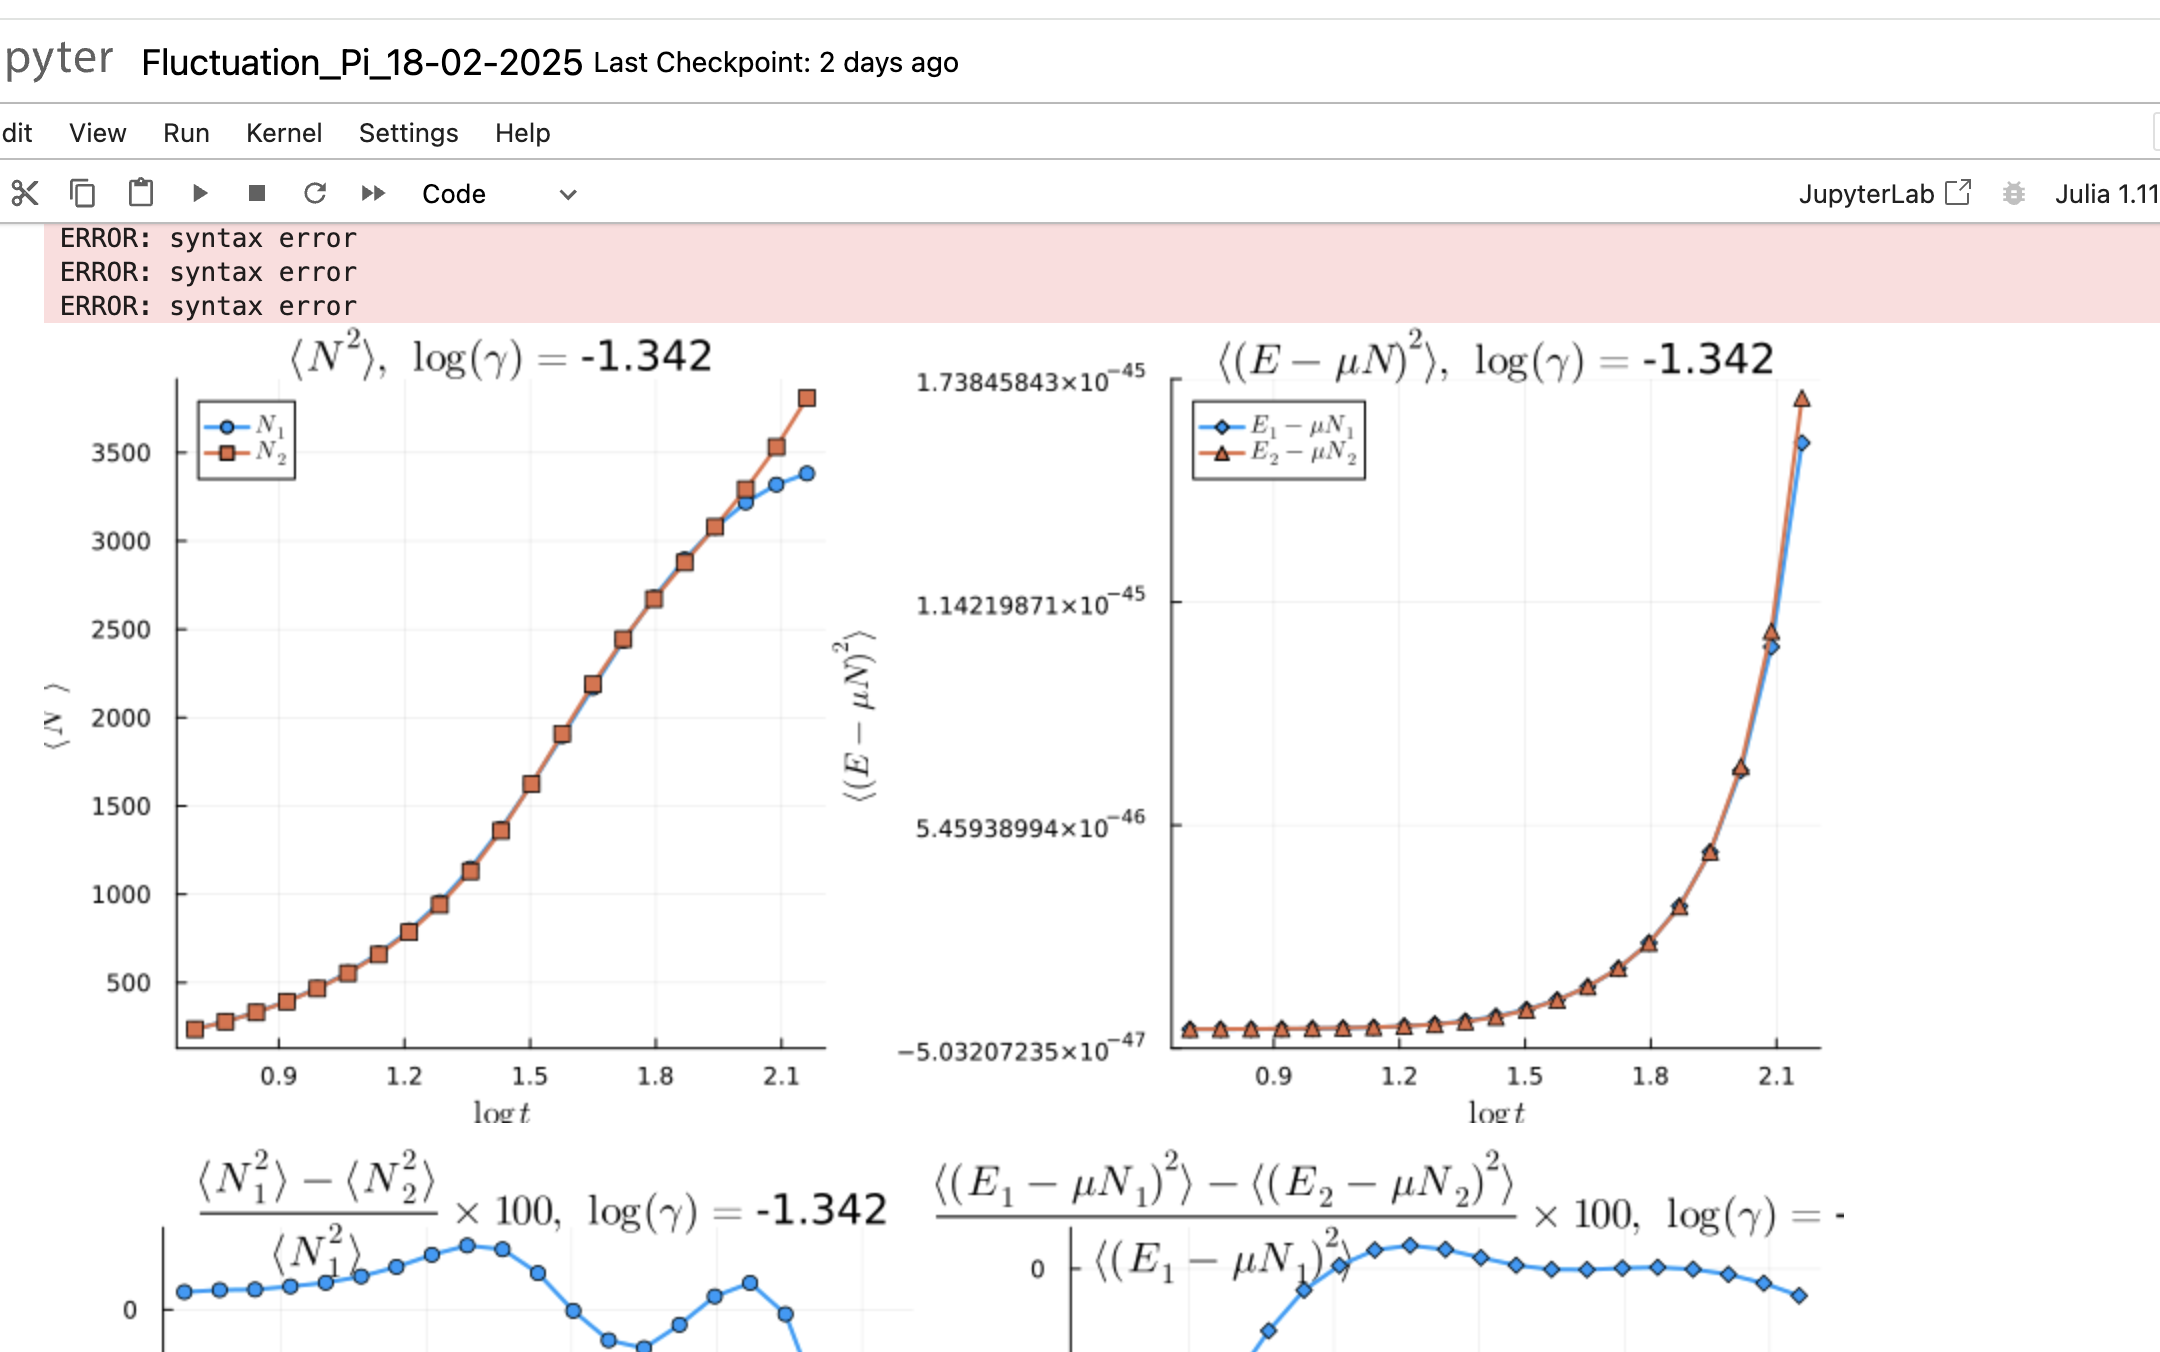
\includegraphics[width=1\textwidth]{Figures/test}

%\begin{aff}
%Donc une a l'ordre un en $\delta \theta (\operator{A}^{(0)})^{-1} %\operator{V}$ 

%\begin{eqnarray*}
%	\langle \delta \Pi ( \theta) \delta \Pi ( \theta') \rangle & = &  ( (\Pi^c_s - \Pi^c)\Pi^c/\Pi^c_s ) ( \theta ) \delta_{\theta, \theta'}/\delta \theta + \mathscr{F}(\theta , \theta' ) ,	
%\end{eqnarray*}

%avec 

%\begin{eqnarray*}
%	\mathscr{F}(\theta , \theta' ) & = & \left [ (\Pi^c_s - \Pi^c )( \theta)  +  (\Pi^c_s - \Pi^c ) ( \theta' )\right ] \frac{\Pi^c}{\Pi^c_s}(\theta)\frac{\Pi^c}{\Pi^c_s}(\theta') \frac{ \Delta( \theta'- \theta )}{ 2 \pi }\\
%	&&  - \left [ (\Pi^c_s - \Pi^c )( \theta)   (\Pi^c_s - \Pi^c ) ( \theta' )\right ] \frac{\Pi^c}{\Pi^c_s}(\theta)\frac{\Pi^c}{\Pi^c_s}(\theta')\int d\theta'' \left (   \frac{ \Pi^c/\Pi^c_s}{\Pi^c_s - \Pi^c} \right )(\theta'') \frac{\Delta(\theta''- \theta)}{2 \pi}\frac{\Delta(\theta''- \theta')}{2 \pi}  	
%\end{eqnarray*}
%\end{aff}



 








 
\subsection{Fonction d’onde $\chi_N$ et Hamiltonien et moment à N corps}
%Dans ce chapitre, nous nous intéressons aux fluctuations de la distribution de rapidité \( \delta \rho \) autour d'une distribution de référence \( \rho^c \), qui maximise la contribution à la fonction de partition des états, exprimée comme une fonctionnelle de la distribution \( \rho \) : 

La fonction de partition des états, s'exprime comme une fonctionnelle de la distribution \( \rho \) : 

\begin{eqnarray*}
	\Xi & = & \sum_\rho \exp \left( -\mathcal{A}(\rho) \right).
\end{eqnarray*}  

Dans la section {\em \bf Entropie de Yang-Yang} (\ref{??}), l'action \( \mathcal{A}(\rho) \) s'écrit sous la forme :  

\begin{eqnarray*}
	\mathcal{A}(\rho) & \doteq & - L\mathcal{S}_{YY}(\rho) + L\int f(\theta) \rho (\theta) \, d\theta,		
\end{eqnarray*}  

où \( \mathcal{S}_{YY} \) est la fonctionnelle d'entropie de Yang-Yang, définie dans (\ref{??}), et \( f \) est la fonction paramétrant les charges, introduite dans (\ref{??}).  

Dans cette même section {\em \bf Entropie de Yang-Yang} (\ref{??}), nous avons établi un lien entre \( f \) et distribution de référence \( \rho^c \), qui maximise la contribution à la fonction de partition des états .\\

On veux tester si nos experience est décrit pas un GGE. Pour cela nous nous intéressons aux fluctuations de la distribution de rapidité \( \delta \rho \) autour \( \rho^c \).

%Nous poursuivons à présent avec cette définition de l'action de classe $\mathcal{C}^2$ et admetant une distribution critique $\rho^c$ tel que sa différentielle en ce point critique soit nulle $d\mathcal{A}_{\rho^c} = 0 $ (\ref{??}) de sorte que d'aprés la formule de Taylor-Youg %afin de déterminer les fluctuations autour de \( \Pi^c \). Pour cela, nous réécrivons l'action sous la forme :  

Nous poursuivons à présent avec cette définition de l'action de classe $\mathcal{C}^2$ et admetant une distribution critique $\rho^c$ tel que sa différentielle en ce point critique soit nulle $d\mathcal{A}_{\rho^c} = 0 $ (\ref{??}) de sorte que d'aprés la formule de Taylor-Youg %afin de déterminer les fluctuations autour de \( \Pi^c \). Pour cela, nous réécrivons l'action sous la forme :  

\begin{eqnarray*}  
	\mathcal{A}(\rho^c + \delta \rho) & \underset{ \delta \rho \to 0 }{=} & \mathcal{A}(\rho^c)  + \frac{1}{2} \left. \frac{\delta^2 \mathcal{A}}{\delta \rho^2} \right|_{\rho^c} (\delta \rho) + \mathcal{O}((\delta \rho)^3),  
\end{eqnarray*}  

une expression quadratique pour l'action à l'ordre dominant en \( \delta \Pi \) avec $\left. \frac{\delta^2 \mathcal{A}}{\delta \rho^2} \right|_{\rho^c}$ la forme quadratique définie positive (Fig (\ref{fig.fluctu.A})).

\begin{figure}[H]
	\centering 
	\begin{tikzpicture}
		\begin{scope}[shift={(0,0)}]
			\begin{scope}[transform canvas={scale=0.6}]
				% Définition des couleurs avec les codes HTML
\definecolor{colorOne}{HTML}{443E46}
\definecolor{colorTwo}{HTML}{F6DEB8}
\definecolor{colorThree}{HTML}{908CA4}
\definecolor{colorFour}{HTML}{57659E}
\definecolor{colorFive}{HTML}{C57284}
\definecolor{colorSix}{HTML}{FF5B69}

% Raccourcis pour les couleurs
\def\colorOne{colorOne}
\def\colorTwo{colorTwo}
\def\colorThree{colorThree}
\def\colorFour{colorFour}
\def\colorFive{colorFive}
\def\colorSix{colorSix}

\def\colorslide{blue!50!black}



\begin{scope}
	% Tracer une courbe lisse entre des points
	\draw[shift={(0,0)} ,\colorOne]
		(-1 , 0 ) edge [thick,line width=0.8ex , ->,>=triangle 45  , \colorOne] node [pos = 1 , below ]{\huge$\rho$}( 5  , 0 )
	;
	\draw[shift={(0,0)}, color=\colorOne]
		(0, -1.0 ) edge [thick,line width=0.8ex , ->,>=triangle 45  ]node [pos=0.9,left=0.2cm ]{\huge$\mathcal{A}(\rho)$}( 0  , 5 )
	;
	\draw[]
		(2.5, 0.12 ) edge [thick,line width=0.8ex ,\colorThree ]node [pos=1,below  ]{\huge$\rho^c$} (2.5, -0.12 )	
	;
	
	\draw[]
		(2.5, -0.12 ) edge [thick,line width=0.4ex , dashed, \colorThree ] (2.5, 5.5 )
		(1.5, 1 ) edge [thick,line width=0.4ex , <->,>=triangle 45  , \colorThree ] (3.5, 1 )
		(-0.3,1) edge [thick,line width=0.4ex  , \colorThree ] node [pos=0,left ]{\huge$\mathcal{A}(\rho^c)$} (0.3, 1 )	
	;
    \draw[thick, line width=0.8ex , \colorFour] plot[smooth, tension=0.7] coordinates {
        (1, 5) (1.6 , 3 ) (2.5, 1) (3.5 , 3 )  (4, 5)
    };		
	
\end{scope}

	
			
			\end{scope}
			
			\draw[color = red , scale = 0.5 , draw = none  ] (-2 , -1) rectangle (5, 6) ; 	
		\end{scope}
		
		\begin{scope}[shift={(19,-1)}]
			\begin{scope}[transform canvas={scale=0.6}]
				% Définition des couleurs avec les codes HTML
\definecolor{colorOne}{HTML}{443E46}
\definecolor{colorTwo}{HTML}{F6DEB8}
\definecolor{colorThree}{HTML}{908CA4}
\definecolor{colorFour}{HTML}{57659E}
\definecolor{colorFive}{HTML}{C57284}
\definecolor{colorSix}{HTML}{FF5B69}

% Raccourcis pour les couleurs
\def\colorOne{colorOne}
\def\colorTwo{colorTwo}
\def\colorThree{colorThree}
\def\colorFour{colorFour}
\def\colorFive{colorFive}
\def\colorSix{colorSix}

\def\colorslide{blue!50!black}

\def\Occupation{
	\def\traitx{0.3}
	\def\traity{0.5}
	\draw[shift={(0,0)}]
		(-13.5 , 0 ) edge [thick,line width=0.8ex ]( -3.2  , 0 )
		( -3.2 - \traitx  , 0 - \traity ) edge [thick,line width=0.8ex ]( -3.2 + \traitx  , 0 + \traity  )
		( -2.8 - \traitx  , 0 - \traity ) edge [thick,line width=0.8ex ]( -2.8 + \traitx  , 0 + \traity  )
		(-2.8 , 0 ) edge [thick,line width=0.8ex ](2.8  , 0 )
		( 2.8 - \traitx  , 0 - \traity ) edge [thick,line width=0.8ex ]( 2.8 + \traitx  , 0 + \traity  )
		( 3.2 - \traitx  , 0 - \traity ) edge [thick,line width=0.8ex ]( 3.2 + \traitx  , 0 + \traity  )
		(3.2, 0 ) edge [thick,line width=0.8ex,->,>=triangle 45 , color = black ]node [pos=1.01,below  ]{\huge$\theta$}	( 13  , 0 )
	;
	\draw[shift={(0,0)}, color=\colorOne]
		(-10.5 , -1.5 ) edge [thick,line width=0.8ex , ->,>=triangle 45  ]( -10.5  , 4.5 )
	;
		
	\foreach \r in {1 , ... , 3 } {
%		\draw[
%		decoration={
%		markings,
%    	mark connection node=my node,
%    	mark=at position 0 with{\node [blue,transform shape] (my node) {\large \r};}},
%		color=gray, thick, 
%		line width=0.5ex] decorate { 
%            (-11.0, \r) -- (-10.1, \r )}
%        ;
        \draw[
			color=\colorOne,
			] 
            (-11.0, \r) edge[color=\colorThree , thick,line width=0.5ex] node [pos=-0.5 ]{\large\color{\colorFour} $\frac{\r}{\delta \theta}$ } (-10.3, \r )
        	;
	
	}
	

	
	% Graduation abcsisse 
	% Définitions des listes
% Definitions of the lists
\def\listetuple{-9/\theta_{1}, -8/\theta_{2} , -5/\theta_{3} , -2/\theta_{a-1} , 0/\theta_{a} , 1/\theta_{a+1} , 2/\theta_{a+2} ,  5/\theta_{N-4} , 7/\theta_{N-3},8/\theta_{N-1},9/\theta_{N} }
\def\listetrais{-12 , -11, -10, -9 , -8 , -7 ,  -6 , -5, -4.5,-4, -2 , -1, 0 , 0.5, 1, 2, 4 , 5 ,  6 , 7 , 8 ,8.5, 9 ,  10 , 11, 12 }

% Loop over listetrais
\foreach \r in \listetrais {
    % Initialize found variable to zero
    % Initialize found variable to zero
    %\pgfmathsetmacro\found{0}
    \global\def\found{0}
    \xdef\nomtheta{}
    
    % Check if \r is in listetuple
    \foreach \x/\y in \listetuple { 
        \ifdim \r pt=\x pt % If \r matches any \x in listetuple
            \global\def\found{1} ;
            \xdef\nomtheta{\y} % Set \nomtheta to the corresponding \y
            %\pgfmathsetmacro\found{1} % Set found to 1            
            %\global\pgfmathsetmacro\found{1}
        \fi
    }
    
    %\node [circle, draw, red] (A) at (\r, 2) {\found , $\nomtheta$};
    
    % Draw the line and display \nomtheta if found
    \ifnum\found=1
        \draw[color=\colorOne, thick, line width=0.5ex] 
            (\r, -0.3) -- (\r, 0.3) node[red , pos=-0.5] {\large $\nomtheta$};
         \filldraw[line width=0.5ex, color=\colorSix, outer color=\colorSix, inner color=\colorSix] 
            (\r, 0) circle (4pt);
    \else 
        % Draw without \nomtheta and add a blue circle if not found
        \draw[color=\colorOne, thick, line width=0.5ex] 
            (\r, -0.3) -- (\r, 0.3);
        \filldraw[line width=0.5ex, color=\colorSix, outer color=\colorTwo, inner color=\colorTwo] 
            (\r, 0) circle (4pt); 
    \fi
}

\def\listetrais{-9.5/\theta_{i-1}/2/3, -6.5/\theta_{i}/1/4  ,   -1.5/\theta_{j}/2/4 , 1.5/\theta_{j+1}/-1/3 , 3.5/\theta_{\ell-1}/1/3 , 6.5/\theta_{\ell}/3/4 , 9.5/\theta(\theta_{\ell+1})/-1/3 };



\foreach \r/\nomx/\y/\ys in \listetrais {
	\draw[
		decoration={
		markings,
    	mark connection node=my node,
    	mark=at position .5 with{\node [blue,transform shape] (my node) {\large \color{\colorFour} $\nomx$};}},
		color=\colorThree , thick, 
		line width=0.5ex] decorate { 
            (\r, 0.12) -- (\r, -1.2)}
        ;
     
     \ifdim \y pt > -1 pt 
     	\draw[
			decoration={
			markings,
    		mark connection node=my node,
    		mark=at position .5 with{\node [blue,transform shape] (my node) {\large \color{\colorFour} $\Pi(\nomx) $};}},
			color=\colorThree, thick, 
			line width=0.5ex] decorate { 
            (\r, \y) -- (\r +3, \y)}
        ;
        \draw[
			decoration={
			markings,
    		mark connection node=my node,
    		mark=at position .5 with{\node [blue,transform shape] (my node) {\large \color{\colorFive} $\Pi_s(\nomx) $};}},
			color=\colorFive, thick, 
			line width=0.5ex] decorate { 
            (\r, \ys) -- (\r +3, \ys)}
        ;
     \fi 
     \ifdim \r pt= -1.5 pt
     	\draw[
     		decoration={
			markings,
    		mark connection node=my node,
    		mark=at position .5 with{\node [blue,transform shape] (my node) {\large \color{\colorFour}  $\delta \theta $};},
    		%mark=at position 0.1  with {\arrow[blue, line width=0.5ex]{<}},
    		%mark=at position 1  with {\arrow[blue, line width=0.5ex]{>}}
    		},
        	color=\colorThree,
        	thick,
        	line width=0.5ex,
        	%arrows={Computer Modern Rightarrow[line cap=round]-Computer Modern Rightarrow[line cap=round]}
   			](\r, -1.2) edge[arrows={Computer Modern Rightarrow[line cap=round]-}] (\r + 0.4, -1.2)decorate {
    		(\r, -1.2) -- (\r + 3, -1.2)}(\r + 2, -1.2) edge[arrows={-Computer Modern Rightarrow[line cap=round]}] (\r + 3, -1.2)
    		;
    \fi
			
	
}


			
}


\begin{scope}
	%\draw[help lines , width=1.5ex] (-8,-3) grid (8,3);\draw[help lines ,width=0.5ex , opacity = 0.5] (-3,-3) grid[step=0.1] (3,3));
	
	%\draw[help lines] 
	%	(-3,-3) edge[width=1.5ex] grid (3,3)	
	%	(-3,-3) edge[width=0.5ex , opacity = 0.5] grid (3,3)	
	%;
	\begin{scope}[shift={(0,1)},rotate=0,opacity=1,color=black]
		\Occupation	
		
		%\node[anchor=east, font=\bfseries] at (-11, 0) {\color{red}\large (T = 0 )} ;	
	\end{scope}
	
	
	
	
	\begin{scope}[shift={(-10.5,7)},rotate=0,opacity=1,color=black]
	
	\begin{scope}[shift={(-0,0)},rotate=0,opacity=1,color=black]
	
		\draw[shift={(0,0)} ,line width=1ex,rounded corners = 1ex,color=\colorOne , opacity =1 ,fill=\colorOne!00 , pattern={north east lines} , pattern color=\colorOne!00 ]
			(0 , -1 ) rectangle (5,1)
		;
		

		\begin{scope}[shift={(0.5,0.5)}]
			\draw[color=\colorOne, thick, line width=0.5ex] 
            (0, -0.3) -- (0, 0.3) ;
            \filldraw[line width=0.5ex, color=\colorSix, outer color=\colorSix, inner color=\colorSix] 
            (0, 0) circle (4pt);
            
            \node[anchor=west, font=\bfseries] at (0.2, 0) {\color{\colorSix}\large : quasi-particule};
		\end{scope}
		
		\begin{scope}[shift={(0.5,-0.5)}]
			\draw[color=\colorOne, thick, line width=0.5ex] 
            (0, -0.3) -- (0, 0.3) ;
            \filldraw[line width=0.5ex, color=\colorSix, outer color=\colorTwo, inner color=\colorTwo] 
            (0, 0) circle (4pt);
            
            \node[anchor=west, font=\bfseries] at (0.2, 0) {\color{\colorSix}\large : hole};
		\end{scope}

	\end{scope}
	
	\begin{scope}[shift={(6,0)},rotate=0,opacity=1,color=black]	
		
		\draw[shift={(0,0)} ,line width=1ex,rounded corners = 1ex,color=\colorOne , opacity =1 ,fill=\colorOne!00 , pattern={north east lines} , pattern color=\colorOne!00 ]
			(0 , -1 ) rectangle (7.5,1)
		;
		
		\node[anchor=west] at (0.5, 0.5) {\color{\colorFour}\large $\Pi$ };\node[anchor=west, font=\bfseries] at (1, 0.5) {\color{\colorFour}\large : quasi-particule distribution};
		
		\node[anchor=west] at (0.5, -0.5) {\color{\colorFour}\large $\Pi_h$ };\node[anchor=west, font=\bfseries] at (1, -0.5) {\color{\colorFour}\large  : hole distribution};
		
	\end{scope}
	
	\begin{scope}[shift={(14.5,0)},rotate=0,opacity=1,color=black]	
		
		\draw[shift={(0,0)} ,line width=1ex,rounded corners = 1ex,color=\colorOne , opacity =1 ,fill=\colorOne!00 , pattern={north east lines} , pattern color=\colorOne!00 ]
			(0 , -0.5 ) rectangle (7.0,0.5)
		;
		
		\node[anchor=west] at (0.2, 0) {\color{\colorFour}\large ${\color{\colorFive}\Pi_s} = \Pi + \Pi_h $ } node[anchor=west , font=\bfseries] at (3.1 , 0 )  {\color{\colorFour}\large {\color{\colorFive} : density of states}};
		
	\end{scope}
	
	
	\end{scope}


		
	
\end{scope}

	
			
			\end{scope}
			\begin{scope}[scale=1]
				\draw[color = red , scale = 1 , draw = none  ] (-1 , -1) rectangle (5, 5) ; 
			\end{scope}	
		\end{scope}

		
				
			
	\end{tikzpicture}	
	\captionsetup{skip=10pt} % Ajoute de l’espace après la légende
	\label{fig.fluctu.A}
\end{figure}


On discrétise l'axe des rapidités en  petite cellule de rapidité $[\theta, \theta+\delta\theta]$, qui contient $L\rho(\theta) \delta \theta$ rapidités. 
	



Avec ces petites tranches, la forme quadratique s’écrit :

\begin{eqnarray*}
    \left. \frac{\delta^2 \mathcal{A}}{{\delta \rho}^2} \right|_{\rho^c}(\delta \rho ) &=&  \sum_{a,b \mid \text{tranche}}  
    \delta \rho(\theta_a)  \frac{\partial^2 \mathcal{A}}{\partial \delta \rho(\theta_a) \partial \delta \rho(\theta_b) } (\rho^c)  \delta \rho(\theta_b).
\end{eqnarray*}
Les fluctuations s’écrivent donc :

\begin{eqnarray*}
    \langle \delta \rho ( \theta) \delta \rho ( \theta') \rangle &=&  
    \frac{ \int d\delta \rho \, \delta \rho(\theta) \delta \rho ( \theta') 
    \exp \left( - \frac{1}{2} \sum_{a,b \mid \text{tranche}}  
    \delta \rho(\theta_a) \frac{\partial^2 \mathcal{A}}{\partial \delta \rho(\theta_a) \partial \delta \rho(\theta_b) } (\rho^c)  \delta \rho(\theta_b) \right) }
    { \int d\delta \Pi  
    \exp \left( - \frac{1}{2} \sum_{a,b \mid \text{tranche}}  
    \delta \rho(\theta_a) \frac{\partial^2 \mathcal{A}}{\partial \delta \rho(\theta_a) \partial \delta \rho(\theta_b) } (\rho^c)  \delta \rho(\theta_b) \right) } \\
    &=& \left( \mathbf{A}^{-1} \right)_{\theta , \theta'}
\end{eqnarray*}


\begin{aff}

\begin{eqnarray*}
	\langle \delta \rho ( \theta) \delta \rho ( \theta') \rangle &=& 	\left( \mathbf{A}^{-1} \right)_{\theta , \theta'}
\end{eqnarray*}

	
avec la  {\em matrice hessienne} $\mathbf{A}_{\theta , \theta'} \equiv \frac{\partial^2 \mathcal{A}}{\partial \delta \rho(\theta) \partial \delta \rho(\theta') }(\rho^c)$, au point critique/ qui maximise la probabilité  $\rho^c=\rho^c_s \nu^c $, s'écrit

\begin{eqnarray*}
	\operator{A} & = & \operator{A}^{(0)} + \delta \theta \operator{V}
\end{eqnarray*}

avec 

\begin{eqnarray*}
	A^{(0)}_{\theta , \theta'}  & = &  L\delta \theta \left ( \frac{ 1}{\rho^c_s ( 1  - \nu^c ) \nu^c } \right )(\theta)    \delta({\theta - \theta '})	,\\
	V_{\theta , \theta'}  &= & L \delta \theta \left \{ - \left [ \left ( \frac{1}{\rho^c_s( 1 - \nu^c) } \right ) ( \theta)  +  \left ( \frac{1}{\rho^c_s( 1 - \nu^c) } \right ) ( \theta' )\right ] \frac{ \Delta( \theta'- \theta )}{ 2 \pi } + \int d\theta''  \left ( \frac{\nu^c}{\rho^c_s( 1 - \nu^c) } \right )(\theta'') \frac{\Delta(\theta''- \theta)}{2 \pi}\frac{\Delta(\theta''- \theta')}{2 \pi}   \right \} 	
\end{eqnarray*}

\end{aff}

\subsection{Testes}

\begin{eqnarray*}
	\Delta_{\operator{\mathcal{N}}}^2  & = &  \frac{1}{\beta} \left . \frac{\partial \langle \operator{\mathcal{N}} \rangle}{\partial \mu} \right )_T \\
	\Delta_{\operator{\mathcal{E}}-\mu \operator{\mathcal{N}}}^2  & = &  - \left . \frac{\partial \langle \operator{\mathcal{E}}-\mu \operator{\mathcal{N}} \rangle}{\partial \beta} \right )_\mu 
\end{eqnarray*}

et 

\begin{eqnarray*}
	\Delta_{\operator{\mathcal{N}}}^2  &= & L^2 \int d\theta_a \int d \theta_b \, \langle \delta \rho(\theta_a) \delta \rho(\theta_b) \rangle \\
	\Delta_{\operator{\mathcal{E}}-\mu \operator{\mathcal{N}}}^2  & = & L^2 \int d\theta_a \int d \theta_b \, \left ( - \mu + \frac{1}2 m \theta_a^2  \right  )\left ( - \mu + \frac{1}2 m \theta_b^2  \right  )  \langle \delta \rho(\theta_a) \delta \rho(\theta_b) \rangle
\end{eqnarray*}

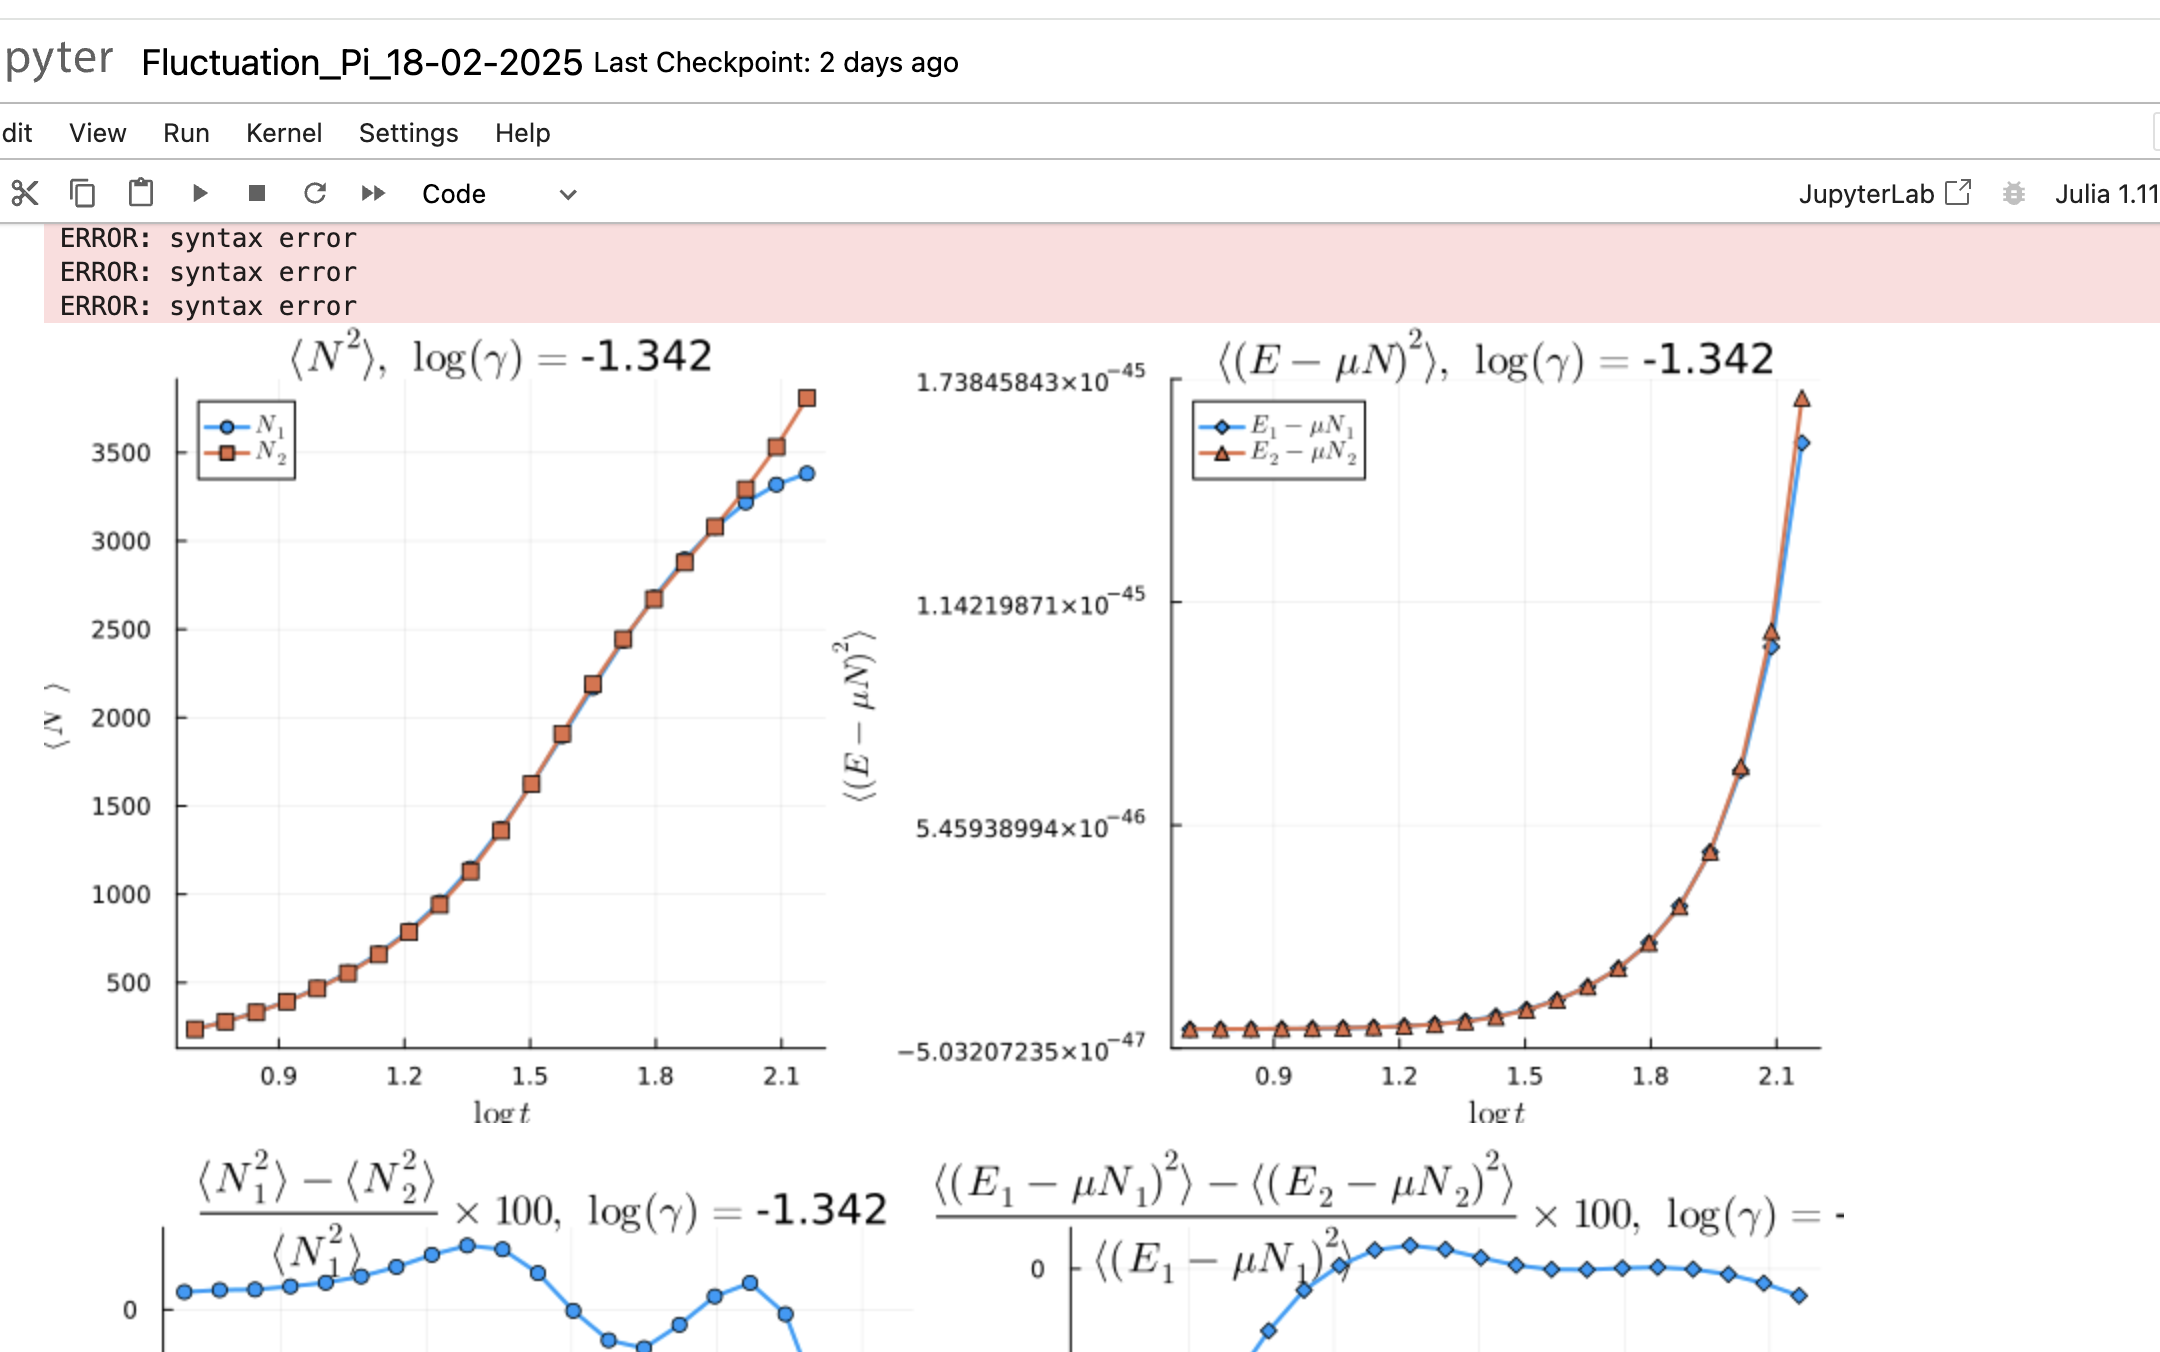
\includegraphics[width=1\textwidth]{Figures/test}

%\begin{aff}
%Donc une a l'ordre un en $\delta \theta (\operator{A}^{(0)})^{-1} %\operator{V}$ 

%\begin{eqnarray*}
%	\langle \delta \Pi ( \theta) \delta \Pi ( \theta') \rangle & = &  ( (\Pi^c_s - \Pi^c)\Pi^c/\Pi^c_s ) ( \theta ) \delta_{\theta, \theta'}/\delta \theta + \mathscr{F}(\theta , \theta' ) ,	
%\end{eqnarray*}

%avec 

%\begin{eqnarray*}
%	\mathscr{F}(\theta , \theta' ) & = & \left [ (\Pi^c_s - \Pi^c )( \theta)  +  (\Pi^c_s - \Pi^c ) ( \theta' )\right ] \frac{\Pi^c}{\Pi^c_s}(\theta)\frac{\Pi^c}{\Pi^c_s}(\theta') \frac{ \Delta( \theta'- \theta )}{ 2 \pi }\\
%	&&  - \left [ (\Pi^c_s - \Pi^c )( \theta)   (\Pi^c_s - \Pi^c ) ( \theta' )\right ] \frac{\Pi^c}{\Pi^c_s}(\theta)\frac{\Pi^c}{\Pi^c_s}(\theta')\int d\theta'' \left (   \frac{ \Pi^c/\Pi^c_s}{\Pi^c_s - \Pi^c} \right )(\theta'') \frac{\Delta(\theta''- \theta)}{2 \pi}\frac{\Delta(\theta''- \theta')}{2 \pi}  	
%\end{eqnarray*}
%\end{aff}



 









\subsection{Exemple : action de $\operator{P}$ sur l’état $\vert \psi_N\rangle$}
%Dans ce chapitre, nous nous intéressons aux fluctuations de la distribution de rapidité \( \delta \rho \) autour d'une distribution de référence \( \rho^c \), qui maximise la contribution à la fonction de partition des états, exprimée comme une fonctionnelle de la distribution \( \rho \) : 

La fonction de partition des états, s'exprime comme une fonctionnelle de la distribution \( \rho \) : 

\begin{eqnarray*}
	\Xi & = & \sum_\rho \exp \left( -\mathcal{A}(\rho) \right).
\end{eqnarray*}  

Dans la section {\em \bf Entropie de Yang-Yang} (\ref{??}), l'action \( \mathcal{A}(\rho) \) s'écrit sous la forme :  

\begin{eqnarray*}
	\mathcal{A}(\rho) & \doteq & - L\mathcal{S}_{YY}(\rho) + L\int f(\theta) \rho (\theta) \, d\theta,		
\end{eqnarray*}  

où \( \mathcal{S}_{YY} \) est la fonctionnelle d'entropie de Yang-Yang, définie dans (\ref{??}), et \( f \) est la fonction paramétrant les charges, introduite dans (\ref{??}).  

Dans cette même section {\em \bf Entropie de Yang-Yang} (\ref{??}), nous avons établi un lien entre \( f \) et distribution de référence \( \rho^c \), qui maximise la contribution à la fonction de partition des états .\\

On veux tester si nos experience est décrit pas un GGE. Pour cela nous nous intéressons aux fluctuations de la distribution de rapidité \( \delta \rho \) autour \( \rho^c \).

%Nous poursuivons à présent avec cette définition de l'action de classe $\mathcal{C}^2$ et admetant une distribution critique $\rho^c$ tel que sa différentielle en ce point critique soit nulle $d\mathcal{A}_{\rho^c} = 0 $ (\ref{??}) de sorte que d'aprés la formule de Taylor-Youg %afin de déterminer les fluctuations autour de \( \Pi^c \). Pour cela, nous réécrivons l'action sous la forme :  

Nous poursuivons à présent avec cette définition de l'action de classe $\mathcal{C}^2$ et admetant une distribution critique $\rho^c$ tel que sa différentielle en ce point critique soit nulle $d\mathcal{A}_{\rho^c} = 0 $ (\ref{??}) de sorte que d'aprés la formule de Taylor-Youg %afin de déterminer les fluctuations autour de \( \Pi^c \). Pour cela, nous réécrivons l'action sous la forme :  

\begin{eqnarray*}  
	\mathcal{A}(\rho^c + \delta \rho) & \underset{ \delta \rho \to 0 }{=} & \mathcal{A}(\rho^c)  + \frac{1}{2} \left. \frac{\delta^2 \mathcal{A}}{\delta \rho^2} \right|_{\rho^c} (\delta \rho) + \mathcal{O}((\delta \rho)^3),  
\end{eqnarray*}  

une expression quadratique pour l'action à l'ordre dominant en \( \delta \Pi \) avec $\left. \frac{\delta^2 \mathcal{A}}{\delta \rho^2} \right|_{\rho^c}$ la forme quadratique définie positive (Fig (\ref{fig.fluctu.A})).

\begin{figure}[H]
	\centering 
	\begin{tikzpicture}
		\begin{scope}[shift={(0,0)}]
			\begin{scope}[transform canvas={scale=0.6}]
				% Définition des couleurs avec les codes HTML
\definecolor{colorOne}{HTML}{443E46}
\definecolor{colorTwo}{HTML}{F6DEB8}
\definecolor{colorThree}{HTML}{908CA4}
\definecolor{colorFour}{HTML}{57659E}
\definecolor{colorFive}{HTML}{C57284}
\definecolor{colorSix}{HTML}{FF5B69}

% Raccourcis pour les couleurs
\def\colorOne{colorOne}
\def\colorTwo{colorTwo}
\def\colorThree{colorThree}
\def\colorFour{colorFour}
\def\colorFive{colorFive}
\def\colorSix{colorSix}

\def\colorslide{blue!50!black}



\begin{scope}
	% Tracer une courbe lisse entre des points
	\draw[shift={(0,0)} ,\colorOne]
		(-1 , 0 ) edge [thick,line width=0.8ex , ->,>=triangle 45  , \colorOne] node [pos = 1 , below ]{\huge$\rho$}( 5  , 0 )
	;
	\draw[shift={(0,0)}, color=\colorOne]
		(0, -1.0 ) edge [thick,line width=0.8ex , ->,>=triangle 45  ]node [pos=0.9,left=0.2cm ]{\huge$\mathcal{A}(\rho)$}( 0  , 5 )
	;
	\draw[]
		(2.5, 0.12 ) edge [thick,line width=0.8ex ,\colorThree ]node [pos=1,below  ]{\huge$\rho^c$} (2.5, -0.12 )	
	;
	
	\draw[]
		(2.5, -0.12 ) edge [thick,line width=0.4ex , dashed, \colorThree ] (2.5, 5.5 )
		(1.5, 1 ) edge [thick,line width=0.4ex , <->,>=triangle 45  , \colorThree ] (3.5, 1 )
		(-0.3,1) edge [thick,line width=0.4ex  , \colorThree ] node [pos=0,left ]{\huge$\mathcal{A}(\rho^c)$} (0.3, 1 )	
	;
    \draw[thick, line width=0.8ex , \colorFour] plot[smooth, tension=0.7] coordinates {
        (1, 5) (1.6 , 3 ) (2.5, 1) (3.5 , 3 )  (4, 5)
    };		
	
\end{scope}

	
			
			\end{scope}
			
			\draw[color = red , scale = 0.5 , draw = none  ] (-2 , -1) rectangle (5, 6) ; 	
		\end{scope}
		
		\begin{scope}[shift={(19,-1)}]
			\begin{scope}[transform canvas={scale=0.6}]
				% Définition des couleurs avec les codes HTML
\definecolor{colorOne}{HTML}{443E46}
\definecolor{colorTwo}{HTML}{F6DEB8}
\definecolor{colorThree}{HTML}{908CA4}
\definecolor{colorFour}{HTML}{57659E}
\definecolor{colorFive}{HTML}{C57284}
\definecolor{colorSix}{HTML}{FF5B69}

% Raccourcis pour les couleurs
\def\colorOne{colorOne}
\def\colorTwo{colorTwo}
\def\colorThree{colorThree}
\def\colorFour{colorFour}
\def\colorFive{colorFive}
\def\colorSix{colorSix}

\def\colorslide{blue!50!black}

\def\Occupation{
	\def\traitx{0.3}
	\def\traity{0.5}
	\draw[shift={(0,0)}]
		(-13.5 , 0 ) edge [thick,line width=0.8ex ]( -3.2  , 0 )
		( -3.2 - \traitx  , 0 - \traity ) edge [thick,line width=0.8ex ]( -3.2 + \traitx  , 0 + \traity  )
		( -2.8 - \traitx  , 0 - \traity ) edge [thick,line width=0.8ex ]( -2.8 + \traitx  , 0 + \traity  )
		(-2.8 , 0 ) edge [thick,line width=0.8ex ](2.8  , 0 )
		( 2.8 - \traitx  , 0 - \traity ) edge [thick,line width=0.8ex ]( 2.8 + \traitx  , 0 + \traity  )
		( 3.2 - \traitx  , 0 - \traity ) edge [thick,line width=0.8ex ]( 3.2 + \traitx  , 0 + \traity  )
		(3.2, 0 ) edge [thick,line width=0.8ex,->,>=triangle 45 , color = black ]node [pos=1.01,below  ]{\huge$\theta$}	( 13  , 0 )
	;
	\draw[shift={(0,0)}, color=\colorOne]
		(-10.5 , -1.5 ) edge [thick,line width=0.8ex , ->,>=triangle 45  ]( -10.5  , 4.5 )
	;
		
	\foreach \r in {1 , ... , 3 } {
%		\draw[
%		decoration={
%		markings,
%    	mark connection node=my node,
%    	mark=at position 0 with{\node [blue,transform shape] (my node) {\large \r};}},
%		color=gray, thick, 
%		line width=0.5ex] decorate { 
%            (-11.0, \r) -- (-10.1, \r )}
%        ;
        \draw[
			color=\colorOne,
			] 
            (-11.0, \r) edge[color=\colorThree , thick,line width=0.5ex] node [pos=-0.5 ]{\large\color{\colorFour} $\frac{\r}{\delta \theta}$ } (-10.3, \r )
        	;
	
	}
	

	
	% Graduation abcsisse 
	% Définitions des listes
% Definitions of the lists
\def\listetuple{-9/\theta_{1}, -8/\theta_{2} , -5/\theta_{3} , -2/\theta_{a-1} , 0/\theta_{a} , 1/\theta_{a+1} , 2/\theta_{a+2} ,  5/\theta_{N-4} , 7/\theta_{N-3},8/\theta_{N-1},9/\theta_{N} }
\def\listetrais{-12 , -11, -10, -9 , -8 , -7 ,  -6 , -5, -4.5,-4, -2 , -1, 0 , 0.5, 1, 2, 4 , 5 ,  6 , 7 , 8 ,8.5, 9 ,  10 , 11, 12 }

% Loop over listetrais
\foreach \r in \listetrais {
    % Initialize found variable to zero
    % Initialize found variable to zero
    %\pgfmathsetmacro\found{0}
    \global\def\found{0}
    \xdef\nomtheta{}
    
    % Check if \r is in listetuple
    \foreach \x/\y in \listetuple { 
        \ifdim \r pt=\x pt % If \r matches any \x in listetuple
            \global\def\found{1} ;
            \xdef\nomtheta{\y} % Set \nomtheta to the corresponding \y
            %\pgfmathsetmacro\found{1} % Set found to 1            
            %\global\pgfmathsetmacro\found{1}
        \fi
    }
    
    %\node [circle, draw, red] (A) at (\r, 2) {\found , $\nomtheta$};
    
    % Draw the line and display \nomtheta if found
    \ifnum\found=1
        \draw[color=\colorOne, thick, line width=0.5ex] 
            (\r, -0.3) -- (\r, 0.3) node[red , pos=-0.5] {\large $\nomtheta$};
         \filldraw[line width=0.5ex, color=\colorSix, outer color=\colorSix, inner color=\colorSix] 
            (\r, 0) circle (4pt);
    \else 
        % Draw without \nomtheta and add a blue circle if not found
        \draw[color=\colorOne, thick, line width=0.5ex] 
            (\r, -0.3) -- (\r, 0.3);
        \filldraw[line width=0.5ex, color=\colorSix, outer color=\colorTwo, inner color=\colorTwo] 
            (\r, 0) circle (4pt); 
    \fi
}

\def\listetrais{-9.5/\theta_{i-1}/2/3, -6.5/\theta_{i}/1/4  ,   -1.5/\theta_{j}/2/4 , 1.5/\theta_{j+1}/-1/3 , 3.5/\theta_{\ell-1}/1/3 , 6.5/\theta_{\ell}/3/4 , 9.5/\theta(\theta_{\ell+1})/-1/3 };



\foreach \r/\nomx/\y/\ys in \listetrais {
	\draw[
		decoration={
		markings,
    	mark connection node=my node,
    	mark=at position .5 with{\node [blue,transform shape] (my node) {\large \color{\colorFour} $\nomx$};}},
		color=\colorThree , thick, 
		line width=0.5ex] decorate { 
            (\r, 0.12) -- (\r, -1.2)}
        ;
     
     \ifdim \y pt > -1 pt 
     	\draw[
			decoration={
			markings,
    		mark connection node=my node,
    		mark=at position .5 with{\node [blue,transform shape] (my node) {\large \color{\colorFour} $\Pi(\nomx) $};}},
			color=\colorThree, thick, 
			line width=0.5ex] decorate { 
            (\r, \y) -- (\r +3, \y)}
        ;
        \draw[
			decoration={
			markings,
    		mark connection node=my node,
    		mark=at position .5 with{\node [blue,transform shape] (my node) {\large \color{\colorFive} $\Pi_s(\nomx) $};}},
			color=\colorFive, thick, 
			line width=0.5ex] decorate { 
            (\r, \ys) -- (\r +3, \ys)}
        ;
     \fi 
     \ifdim \r pt= -1.5 pt
     	\draw[
     		decoration={
			markings,
    		mark connection node=my node,
    		mark=at position .5 with{\node [blue,transform shape] (my node) {\large \color{\colorFour}  $\delta \theta $};},
    		%mark=at position 0.1  with {\arrow[blue, line width=0.5ex]{<}},
    		%mark=at position 1  with {\arrow[blue, line width=0.5ex]{>}}
    		},
        	color=\colorThree,
        	thick,
        	line width=0.5ex,
        	%arrows={Computer Modern Rightarrow[line cap=round]-Computer Modern Rightarrow[line cap=round]}
   			](\r, -1.2) edge[arrows={Computer Modern Rightarrow[line cap=round]-}] (\r + 0.4, -1.2)decorate {
    		(\r, -1.2) -- (\r + 3, -1.2)}(\r + 2, -1.2) edge[arrows={-Computer Modern Rightarrow[line cap=round]}] (\r + 3, -1.2)
    		;
    \fi
			
	
}


			
}


\begin{scope}
	%\draw[help lines , width=1.5ex] (-8,-3) grid (8,3);\draw[help lines ,width=0.5ex , opacity = 0.5] (-3,-3) grid[step=0.1] (3,3));
	
	%\draw[help lines] 
	%	(-3,-3) edge[width=1.5ex] grid (3,3)	
	%	(-3,-3) edge[width=0.5ex , opacity = 0.5] grid (3,3)	
	%;
	\begin{scope}[shift={(0,1)},rotate=0,opacity=1,color=black]
		\Occupation	
		
		%\node[anchor=east, font=\bfseries] at (-11, 0) {\color{red}\large (T = 0 )} ;	
	\end{scope}
	
	
	
	
	\begin{scope}[shift={(-10.5,7)},rotate=0,opacity=1,color=black]
	
	\begin{scope}[shift={(-0,0)},rotate=0,opacity=1,color=black]
	
		\draw[shift={(0,0)} ,line width=1ex,rounded corners = 1ex,color=\colorOne , opacity =1 ,fill=\colorOne!00 , pattern={north east lines} , pattern color=\colorOne!00 ]
			(0 , -1 ) rectangle (5,1)
		;
		

		\begin{scope}[shift={(0.5,0.5)}]
			\draw[color=\colorOne, thick, line width=0.5ex] 
            (0, -0.3) -- (0, 0.3) ;
            \filldraw[line width=0.5ex, color=\colorSix, outer color=\colorSix, inner color=\colorSix] 
            (0, 0) circle (4pt);
            
            \node[anchor=west, font=\bfseries] at (0.2, 0) {\color{\colorSix}\large : quasi-particule};
		\end{scope}
		
		\begin{scope}[shift={(0.5,-0.5)}]
			\draw[color=\colorOne, thick, line width=0.5ex] 
            (0, -0.3) -- (0, 0.3) ;
            \filldraw[line width=0.5ex, color=\colorSix, outer color=\colorTwo, inner color=\colorTwo] 
            (0, 0) circle (4pt);
            
            \node[anchor=west, font=\bfseries] at (0.2, 0) {\color{\colorSix}\large : hole};
		\end{scope}

	\end{scope}
	
	\begin{scope}[shift={(6,0)},rotate=0,opacity=1,color=black]	
		
		\draw[shift={(0,0)} ,line width=1ex,rounded corners = 1ex,color=\colorOne , opacity =1 ,fill=\colorOne!00 , pattern={north east lines} , pattern color=\colorOne!00 ]
			(0 , -1 ) rectangle (7.5,1)
		;
		
		\node[anchor=west] at (0.5, 0.5) {\color{\colorFour}\large $\Pi$ };\node[anchor=west, font=\bfseries] at (1, 0.5) {\color{\colorFour}\large : quasi-particule distribution};
		
		\node[anchor=west] at (0.5, -0.5) {\color{\colorFour}\large $\Pi_h$ };\node[anchor=west, font=\bfseries] at (1, -0.5) {\color{\colorFour}\large  : hole distribution};
		
	\end{scope}
	
	\begin{scope}[shift={(14.5,0)},rotate=0,opacity=1,color=black]	
		
		\draw[shift={(0,0)} ,line width=1ex,rounded corners = 1ex,color=\colorOne , opacity =1 ,fill=\colorOne!00 , pattern={north east lines} , pattern color=\colorOne!00 ]
			(0 , -0.5 ) rectangle (7.0,0.5)
		;
		
		\node[anchor=west] at (0.2, 0) {\color{\colorFour}\large ${\color{\colorFive}\Pi_s} = \Pi + \Pi_h $ } node[anchor=west , font=\bfseries] at (3.1 , 0 )  {\color{\colorFour}\large {\color{\colorFive} : density of states}};
		
	\end{scope}
	
	
	\end{scope}


		
	
\end{scope}

	
			
			\end{scope}
			\begin{scope}[scale=1]
				\draw[color = red , scale = 1 , draw = none  ] (-1 , -1) rectangle (5, 5) ; 
			\end{scope}	
		\end{scope}

		
				
			
	\end{tikzpicture}	
	\captionsetup{skip=10pt} % Ajoute de l’espace après la légende
	\label{fig.fluctu.A}
\end{figure}


On discrétise l'axe des rapidités en  petite cellule de rapidité $[\theta, \theta+\delta\theta]$, qui contient $L\rho(\theta) \delta \theta$ rapidités. 
	



Avec ces petites tranches, la forme quadratique s’écrit :

\begin{eqnarray*}
    \left. \frac{\delta^2 \mathcal{A}}{{\delta \rho}^2} \right|_{\rho^c}(\delta \rho ) &=&  \sum_{a,b \mid \text{tranche}}  
    \delta \rho(\theta_a)  \frac{\partial^2 \mathcal{A}}{\partial \delta \rho(\theta_a) \partial \delta \rho(\theta_b) } (\rho^c)  \delta \rho(\theta_b).
\end{eqnarray*}
Les fluctuations s’écrivent donc :

\begin{eqnarray*}
    \langle \delta \rho ( \theta) \delta \rho ( \theta') \rangle &=&  
    \frac{ \int d\delta \rho \, \delta \rho(\theta) \delta \rho ( \theta') 
    \exp \left( - \frac{1}{2} \sum_{a,b \mid \text{tranche}}  
    \delta \rho(\theta_a) \frac{\partial^2 \mathcal{A}}{\partial \delta \rho(\theta_a) \partial \delta \rho(\theta_b) } (\rho^c)  \delta \rho(\theta_b) \right) }
    { \int d\delta \Pi  
    \exp \left( - \frac{1}{2} \sum_{a,b \mid \text{tranche}}  
    \delta \rho(\theta_a) \frac{\partial^2 \mathcal{A}}{\partial \delta \rho(\theta_a) \partial \delta \rho(\theta_b) } (\rho^c)  \delta \rho(\theta_b) \right) } \\
    &=& \left( \mathbf{A}^{-1} \right)_{\theta , \theta'}
\end{eqnarray*}


\begin{aff}

\begin{eqnarray*}
	\langle \delta \rho ( \theta) \delta \rho ( \theta') \rangle &=& 	\left( \mathbf{A}^{-1} \right)_{\theta , \theta'}
\end{eqnarray*}

	
avec la  {\em matrice hessienne} $\mathbf{A}_{\theta , \theta'} \equiv \frac{\partial^2 \mathcal{A}}{\partial \delta \rho(\theta) \partial \delta \rho(\theta') }(\rho^c)$, au point critique/ qui maximise la probabilité  $\rho^c=\rho^c_s \nu^c $, s'écrit

\begin{eqnarray*}
	\operator{A} & = & \operator{A}^{(0)} + \delta \theta \operator{V}
\end{eqnarray*}

avec 

\begin{eqnarray*}
	A^{(0)}_{\theta , \theta'}  & = &  L\delta \theta \left ( \frac{ 1}{\rho^c_s ( 1  - \nu^c ) \nu^c } \right )(\theta)    \delta({\theta - \theta '})	,\\
	V_{\theta , \theta'}  &= & L \delta \theta \left \{ - \left [ \left ( \frac{1}{\rho^c_s( 1 - \nu^c) } \right ) ( \theta)  +  \left ( \frac{1}{\rho^c_s( 1 - \nu^c) } \right ) ( \theta' )\right ] \frac{ \Delta( \theta'- \theta )}{ 2 \pi } + \int d\theta''  \left ( \frac{\nu^c}{\rho^c_s( 1 - \nu^c) } \right )(\theta'') \frac{\Delta(\theta''- \theta)}{2 \pi}\frac{\Delta(\theta''- \theta')}{2 \pi}   \right \} 	
\end{eqnarray*}

\end{aff}

\subsection{Testes}

\begin{eqnarray*}
	\Delta_{\operator{\mathcal{N}}}^2  & = &  \frac{1}{\beta} \left . \frac{\partial \langle \operator{\mathcal{N}} \rangle}{\partial \mu} \right )_T \\
	\Delta_{\operator{\mathcal{E}}-\mu \operator{\mathcal{N}}}^2  & = &  - \left . \frac{\partial \langle \operator{\mathcal{E}}-\mu \operator{\mathcal{N}} \rangle}{\partial \beta} \right )_\mu 
\end{eqnarray*}

et 

\begin{eqnarray*}
	\Delta_{\operator{\mathcal{N}}}^2  &= & L^2 \int d\theta_a \int d \theta_b \, \langle \delta \rho(\theta_a) \delta \rho(\theta_b) \rangle \\
	\Delta_{\operator{\mathcal{E}}-\mu \operator{\mathcal{N}}}^2  & = & L^2 \int d\theta_a \int d \theta_b \, \left ( - \mu + \frac{1}2 m \theta_a^2  \right  )\left ( - \mu + \frac{1}2 m \theta_b^2  \right  )  \langle \delta \rho(\theta_a) \delta \rho(\theta_b) \rangle
\end{eqnarray*}

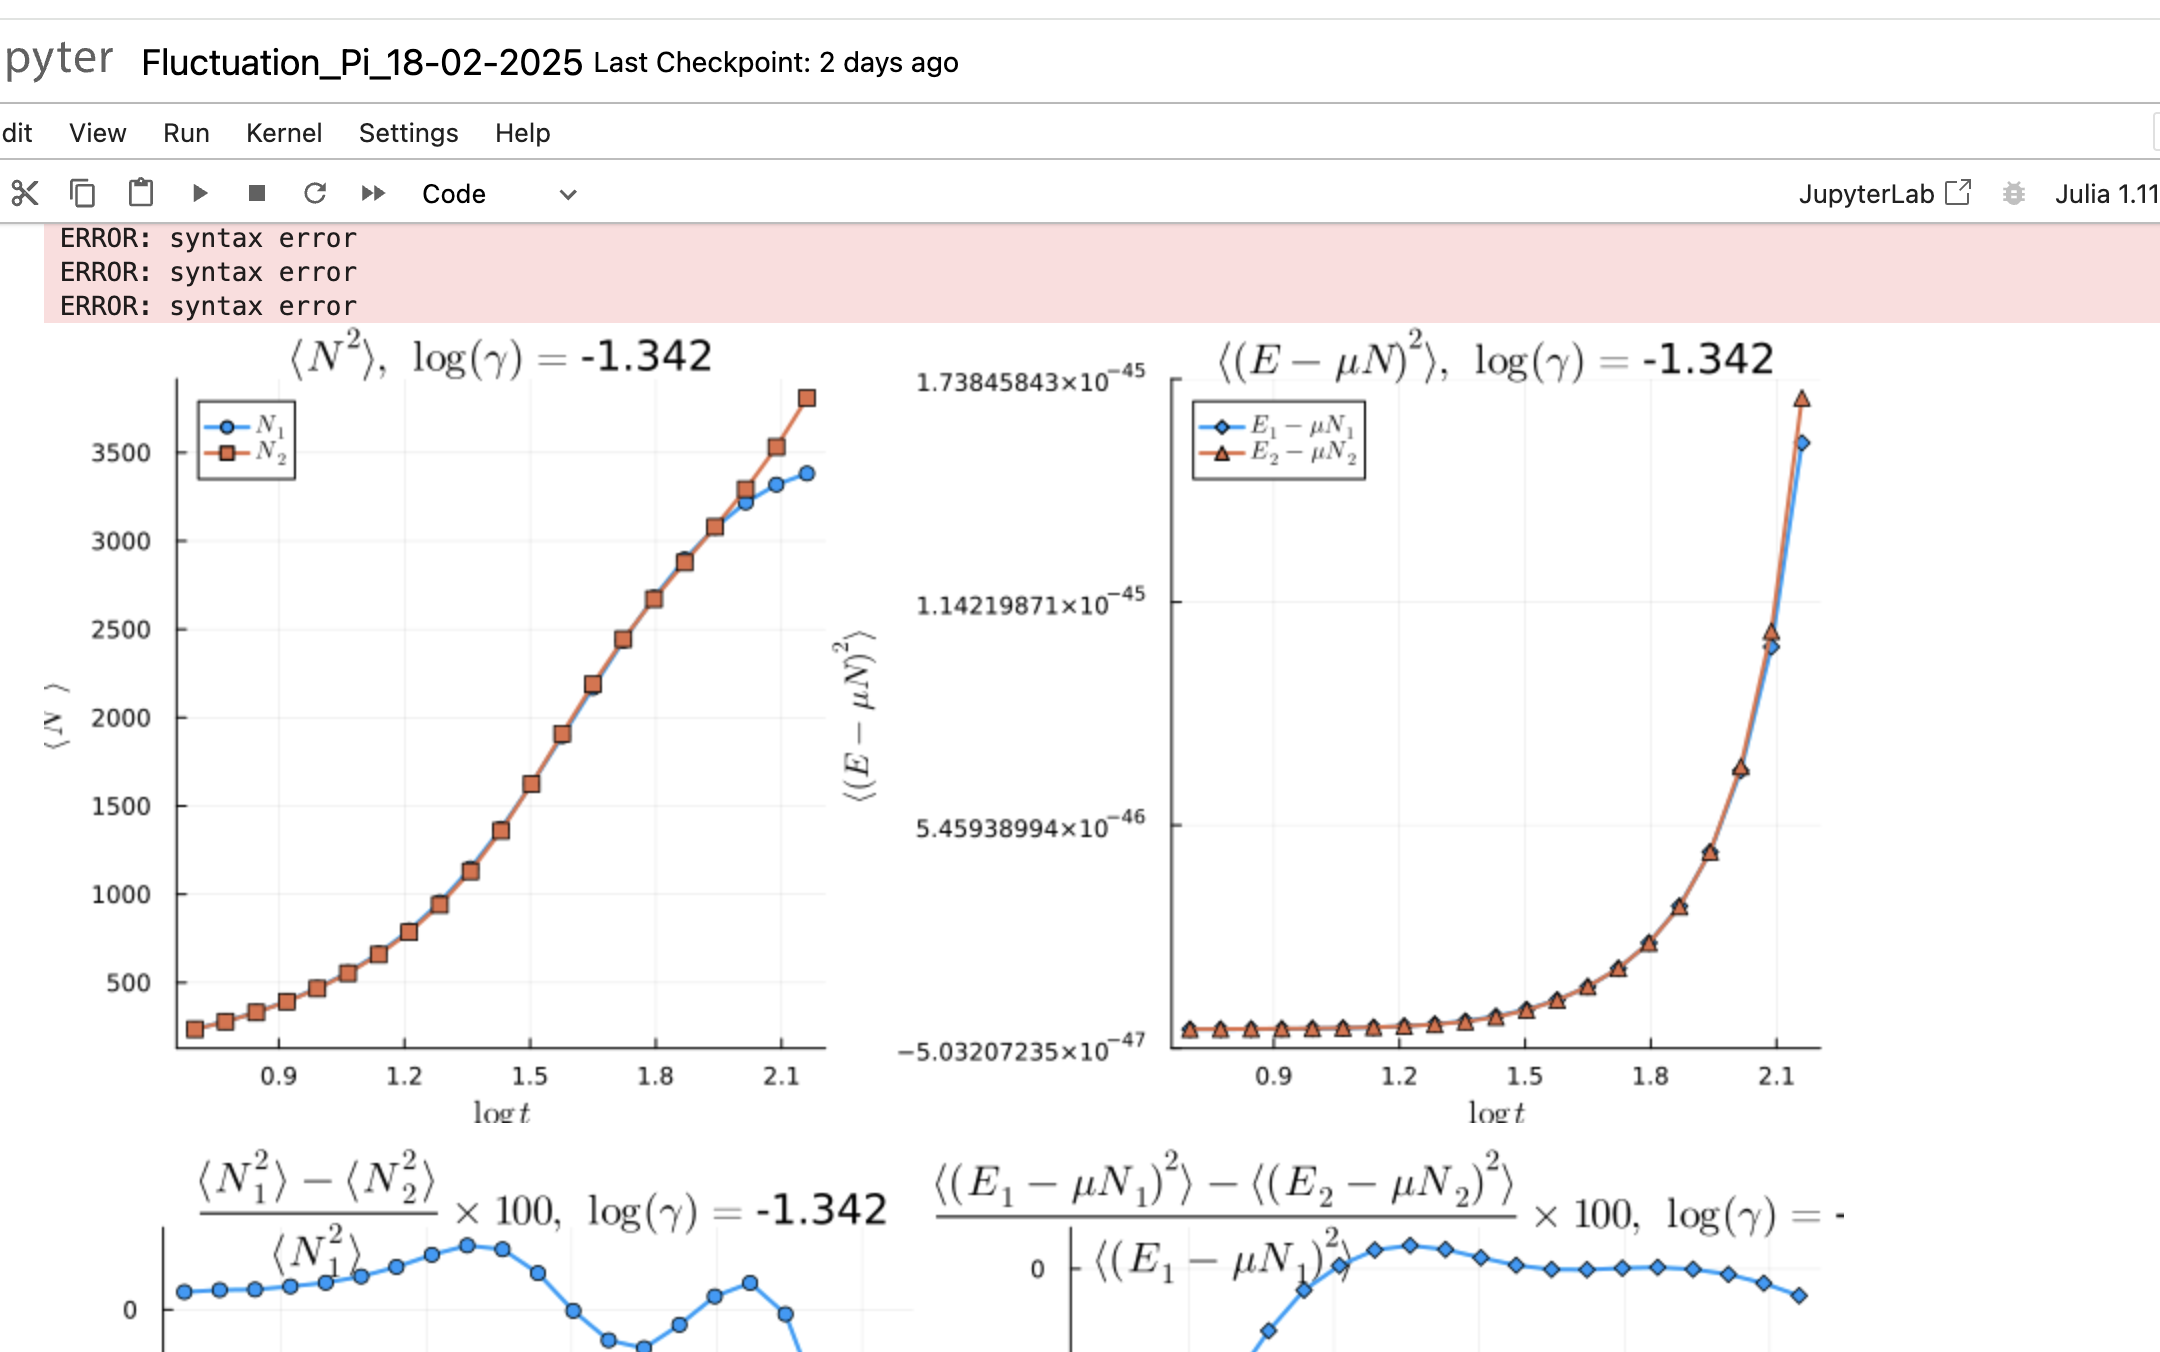
\includegraphics[width=1\textwidth]{Figures/test}

%\begin{aff}
%Donc une a l'ordre un en $\delta \theta (\operator{A}^{(0)})^{-1} %\operator{V}$ 

%\begin{eqnarray*}
%	\langle \delta \Pi ( \theta) \delta \Pi ( \theta') \rangle & = &  ( (\Pi^c_s - \Pi^c)\Pi^c/\Pi^c_s ) ( \theta ) \delta_{\theta, \theta'}/\delta \theta + \mathscr{F}(\theta , \theta' ) ,	
%\end{eqnarray*}

%avec 

%\begin{eqnarray*}
%	\mathscr{F}(\theta , \theta' ) & = & \left [ (\Pi^c_s - \Pi^c )( \theta)  +  (\Pi^c_s - \Pi^c ) ( \theta' )\right ] \frac{\Pi^c}{\Pi^c_s}(\theta)\frac{\Pi^c}{\Pi^c_s}(\theta') \frac{ \Delta( \theta'- \theta )}{ 2 \pi }\\
%	&&  - \left [ (\Pi^c_s - \Pi^c )( \theta)   (\Pi^c_s - \Pi^c ) ( \theta' )\right ] \frac{\Pi^c}{\Pi^c_s}(\theta)\frac{\Pi^c}{\Pi^c_s}(\theta')\int d\theta'' \left (   \frac{ \Pi^c/\Pi^c_s}{\Pi^c_s - \Pi^c} \right )(\theta'') \frac{\Delta(\theta''- \theta)}{2 \pi}\frac{\Delta(\theta''- \theta')}{2 \pi}  	
%\end{eqnarray*}
%\end{aff}



 









\subsection{Aaction de $\operator{H}$ sur l’état $\vert \psi_N\rangle$}
%Dans ce chapitre, nous nous intéressons aux fluctuations de la distribution de rapidité \( \delta \rho \) autour d'une distribution de référence \( \rho^c \), qui maximise la contribution à la fonction de partition des états, exprimée comme une fonctionnelle de la distribution \( \rho \) : 

La fonction de partition des états, s'exprime comme une fonctionnelle de la distribution \( \rho \) : 

\begin{eqnarray*}
	\Xi & = & \sum_\rho \exp \left( -\mathcal{A}(\rho) \right).
\end{eqnarray*}  

Dans la section {\em \bf Entropie de Yang-Yang} (\ref{??}), l'action \( \mathcal{A}(\rho) \) s'écrit sous la forme :  

\begin{eqnarray*}
	\mathcal{A}(\rho) & \doteq & - L\mathcal{S}_{YY}(\rho) + L\int f(\theta) \rho (\theta) \, d\theta,		
\end{eqnarray*}  

où \( \mathcal{S}_{YY} \) est la fonctionnelle d'entropie de Yang-Yang, définie dans (\ref{??}), et \( f \) est la fonction paramétrant les charges, introduite dans (\ref{??}).  

Dans cette même section {\em \bf Entropie de Yang-Yang} (\ref{??}), nous avons établi un lien entre \( f \) et distribution de référence \( \rho^c \), qui maximise la contribution à la fonction de partition des états .\\

On veux tester si nos experience est décrit pas un GGE. Pour cela nous nous intéressons aux fluctuations de la distribution de rapidité \( \delta \rho \) autour \( \rho^c \).

%Nous poursuivons à présent avec cette définition de l'action de classe $\mathcal{C}^2$ et admetant une distribution critique $\rho^c$ tel que sa différentielle en ce point critique soit nulle $d\mathcal{A}_{\rho^c} = 0 $ (\ref{??}) de sorte que d'aprés la formule de Taylor-Youg %afin de déterminer les fluctuations autour de \( \Pi^c \). Pour cela, nous réécrivons l'action sous la forme :  

Nous poursuivons à présent avec cette définition de l'action de classe $\mathcal{C}^2$ et admetant une distribution critique $\rho^c$ tel que sa différentielle en ce point critique soit nulle $d\mathcal{A}_{\rho^c} = 0 $ (\ref{??}) de sorte que d'aprés la formule de Taylor-Youg %afin de déterminer les fluctuations autour de \( \Pi^c \). Pour cela, nous réécrivons l'action sous la forme :  

\begin{eqnarray*}  
	\mathcal{A}(\rho^c + \delta \rho) & \underset{ \delta \rho \to 0 }{=} & \mathcal{A}(\rho^c)  + \frac{1}{2} \left. \frac{\delta^2 \mathcal{A}}{\delta \rho^2} \right|_{\rho^c} (\delta \rho) + \mathcal{O}((\delta \rho)^3),  
\end{eqnarray*}  

une expression quadratique pour l'action à l'ordre dominant en \( \delta \Pi \) avec $\left. \frac{\delta^2 \mathcal{A}}{\delta \rho^2} \right|_{\rho^c}$ la forme quadratique définie positive (Fig (\ref{fig.fluctu.A})).

\begin{figure}[H]
	\centering 
	\begin{tikzpicture}
		\begin{scope}[shift={(0,0)}]
			\begin{scope}[transform canvas={scale=0.6}]
				% Définition des couleurs avec les codes HTML
\definecolor{colorOne}{HTML}{443E46}
\definecolor{colorTwo}{HTML}{F6DEB8}
\definecolor{colorThree}{HTML}{908CA4}
\definecolor{colorFour}{HTML}{57659E}
\definecolor{colorFive}{HTML}{C57284}
\definecolor{colorSix}{HTML}{FF5B69}

% Raccourcis pour les couleurs
\def\colorOne{colorOne}
\def\colorTwo{colorTwo}
\def\colorThree{colorThree}
\def\colorFour{colorFour}
\def\colorFive{colorFive}
\def\colorSix{colorSix}

\def\colorslide{blue!50!black}



\begin{scope}
	% Tracer une courbe lisse entre des points
	\draw[shift={(0,0)} ,\colorOne]
		(-1 , 0 ) edge [thick,line width=0.8ex , ->,>=triangle 45  , \colorOne] node [pos = 1 , below ]{\huge$\rho$}( 5  , 0 )
	;
	\draw[shift={(0,0)}, color=\colorOne]
		(0, -1.0 ) edge [thick,line width=0.8ex , ->,>=triangle 45  ]node [pos=0.9,left=0.2cm ]{\huge$\mathcal{A}(\rho)$}( 0  , 5 )
	;
	\draw[]
		(2.5, 0.12 ) edge [thick,line width=0.8ex ,\colorThree ]node [pos=1,below  ]{\huge$\rho^c$} (2.5, -0.12 )	
	;
	
	\draw[]
		(2.5, -0.12 ) edge [thick,line width=0.4ex , dashed, \colorThree ] (2.5, 5.5 )
		(1.5, 1 ) edge [thick,line width=0.4ex , <->,>=triangle 45  , \colorThree ] (3.5, 1 )
		(-0.3,1) edge [thick,line width=0.4ex  , \colorThree ] node [pos=0,left ]{\huge$\mathcal{A}(\rho^c)$} (0.3, 1 )	
	;
    \draw[thick, line width=0.8ex , \colorFour] plot[smooth, tension=0.7] coordinates {
        (1, 5) (1.6 , 3 ) (2.5, 1) (3.5 , 3 )  (4, 5)
    };		
	
\end{scope}

	
			
			\end{scope}
			
			\draw[color = red , scale = 0.5 , draw = none  ] (-2 , -1) rectangle (5, 6) ; 	
		\end{scope}
		
		\begin{scope}[shift={(19,-1)}]
			\begin{scope}[transform canvas={scale=0.6}]
				% Définition des couleurs avec les codes HTML
\definecolor{colorOne}{HTML}{443E46}
\definecolor{colorTwo}{HTML}{F6DEB8}
\definecolor{colorThree}{HTML}{908CA4}
\definecolor{colorFour}{HTML}{57659E}
\definecolor{colorFive}{HTML}{C57284}
\definecolor{colorSix}{HTML}{FF5B69}

% Raccourcis pour les couleurs
\def\colorOne{colorOne}
\def\colorTwo{colorTwo}
\def\colorThree{colorThree}
\def\colorFour{colorFour}
\def\colorFive{colorFive}
\def\colorSix{colorSix}

\def\colorslide{blue!50!black}

\def\Occupation{
	\def\traitx{0.3}
	\def\traity{0.5}
	\draw[shift={(0,0)}]
		(-13.5 , 0 ) edge [thick,line width=0.8ex ]( -3.2  , 0 )
		( -3.2 - \traitx  , 0 - \traity ) edge [thick,line width=0.8ex ]( -3.2 + \traitx  , 0 + \traity  )
		( -2.8 - \traitx  , 0 - \traity ) edge [thick,line width=0.8ex ]( -2.8 + \traitx  , 0 + \traity  )
		(-2.8 , 0 ) edge [thick,line width=0.8ex ](2.8  , 0 )
		( 2.8 - \traitx  , 0 - \traity ) edge [thick,line width=0.8ex ]( 2.8 + \traitx  , 0 + \traity  )
		( 3.2 - \traitx  , 0 - \traity ) edge [thick,line width=0.8ex ]( 3.2 + \traitx  , 0 + \traity  )
		(3.2, 0 ) edge [thick,line width=0.8ex,->,>=triangle 45 , color = black ]node [pos=1.01,below  ]{\huge$\theta$}	( 13  , 0 )
	;
	\draw[shift={(0,0)}, color=\colorOne]
		(-10.5 , -1.5 ) edge [thick,line width=0.8ex , ->,>=triangle 45  ]( -10.5  , 4.5 )
	;
		
	\foreach \r in {1 , ... , 3 } {
%		\draw[
%		decoration={
%		markings,
%    	mark connection node=my node,
%    	mark=at position 0 with{\node [blue,transform shape] (my node) {\large \r};}},
%		color=gray, thick, 
%		line width=0.5ex] decorate { 
%            (-11.0, \r) -- (-10.1, \r )}
%        ;
        \draw[
			color=\colorOne,
			] 
            (-11.0, \r) edge[color=\colorThree , thick,line width=0.5ex] node [pos=-0.5 ]{\large\color{\colorFour} $\frac{\r}{\delta \theta}$ } (-10.3, \r )
        	;
	
	}
	

	
	% Graduation abcsisse 
	% Définitions des listes
% Definitions of the lists
\def\listetuple{-9/\theta_{1}, -8/\theta_{2} , -5/\theta_{3} , -2/\theta_{a-1} , 0/\theta_{a} , 1/\theta_{a+1} , 2/\theta_{a+2} ,  5/\theta_{N-4} , 7/\theta_{N-3},8/\theta_{N-1},9/\theta_{N} }
\def\listetrais{-12 , -11, -10, -9 , -8 , -7 ,  -6 , -5, -4.5,-4, -2 , -1, 0 , 0.5, 1, 2, 4 , 5 ,  6 , 7 , 8 ,8.5, 9 ,  10 , 11, 12 }

% Loop over listetrais
\foreach \r in \listetrais {
    % Initialize found variable to zero
    % Initialize found variable to zero
    %\pgfmathsetmacro\found{0}
    \global\def\found{0}
    \xdef\nomtheta{}
    
    % Check if \r is in listetuple
    \foreach \x/\y in \listetuple { 
        \ifdim \r pt=\x pt % If \r matches any \x in listetuple
            \global\def\found{1} ;
            \xdef\nomtheta{\y} % Set \nomtheta to the corresponding \y
            %\pgfmathsetmacro\found{1} % Set found to 1            
            %\global\pgfmathsetmacro\found{1}
        \fi
    }
    
    %\node [circle, draw, red] (A) at (\r, 2) {\found , $\nomtheta$};
    
    % Draw the line and display \nomtheta if found
    \ifnum\found=1
        \draw[color=\colorOne, thick, line width=0.5ex] 
            (\r, -0.3) -- (\r, 0.3) node[red , pos=-0.5] {\large $\nomtheta$};
         \filldraw[line width=0.5ex, color=\colorSix, outer color=\colorSix, inner color=\colorSix] 
            (\r, 0) circle (4pt);
    \else 
        % Draw without \nomtheta and add a blue circle if not found
        \draw[color=\colorOne, thick, line width=0.5ex] 
            (\r, -0.3) -- (\r, 0.3);
        \filldraw[line width=0.5ex, color=\colorSix, outer color=\colorTwo, inner color=\colorTwo] 
            (\r, 0) circle (4pt); 
    \fi
}

\def\listetrais{-9.5/\theta_{i-1}/2/3, -6.5/\theta_{i}/1/4  ,   -1.5/\theta_{j}/2/4 , 1.5/\theta_{j+1}/-1/3 , 3.5/\theta_{\ell-1}/1/3 , 6.5/\theta_{\ell}/3/4 , 9.5/\theta(\theta_{\ell+1})/-1/3 };



\foreach \r/\nomx/\y/\ys in \listetrais {
	\draw[
		decoration={
		markings,
    	mark connection node=my node,
    	mark=at position .5 with{\node [blue,transform shape] (my node) {\large \color{\colorFour} $\nomx$};}},
		color=\colorThree , thick, 
		line width=0.5ex] decorate { 
            (\r, 0.12) -- (\r, -1.2)}
        ;
     
     \ifdim \y pt > -1 pt 
     	\draw[
			decoration={
			markings,
    		mark connection node=my node,
    		mark=at position .5 with{\node [blue,transform shape] (my node) {\large \color{\colorFour} $\Pi(\nomx) $};}},
			color=\colorThree, thick, 
			line width=0.5ex] decorate { 
            (\r, \y) -- (\r +3, \y)}
        ;
        \draw[
			decoration={
			markings,
    		mark connection node=my node,
    		mark=at position .5 with{\node [blue,transform shape] (my node) {\large \color{\colorFive} $\Pi_s(\nomx) $};}},
			color=\colorFive, thick, 
			line width=0.5ex] decorate { 
            (\r, \ys) -- (\r +3, \ys)}
        ;
     \fi 
     \ifdim \r pt= -1.5 pt
     	\draw[
     		decoration={
			markings,
    		mark connection node=my node,
    		mark=at position .5 with{\node [blue,transform shape] (my node) {\large \color{\colorFour}  $\delta \theta $};},
    		%mark=at position 0.1  with {\arrow[blue, line width=0.5ex]{<}},
    		%mark=at position 1  with {\arrow[blue, line width=0.5ex]{>}}
    		},
        	color=\colorThree,
        	thick,
        	line width=0.5ex,
        	%arrows={Computer Modern Rightarrow[line cap=round]-Computer Modern Rightarrow[line cap=round]}
   			](\r, -1.2) edge[arrows={Computer Modern Rightarrow[line cap=round]-}] (\r + 0.4, -1.2)decorate {
    		(\r, -1.2) -- (\r + 3, -1.2)}(\r + 2, -1.2) edge[arrows={-Computer Modern Rightarrow[line cap=round]}] (\r + 3, -1.2)
    		;
    \fi
			
	
}


			
}


\begin{scope}
	%\draw[help lines , width=1.5ex] (-8,-3) grid (8,3);\draw[help lines ,width=0.5ex , opacity = 0.5] (-3,-3) grid[step=0.1] (3,3));
	
	%\draw[help lines] 
	%	(-3,-3) edge[width=1.5ex] grid (3,3)	
	%	(-3,-3) edge[width=0.5ex , opacity = 0.5] grid (3,3)	
	%;
	\begin{scope}[shift={(0,1)},rotate=0,opacity=1,color=black]
		\Occupation	
		
		%\node[anchor=east, font=\bfseries] at (-11, 0) {\color{red}\large (T = 0 )} ;	
	\end{scope}
	
	
	
	
	\begin{scope}[shift={(-10.5,7)},rotate=0,opacity=1,color=black]
	
	\begin{scope}[shift={(-0,0)},rotate=0,opacity=1,color=black]
	
		\draw[shift={(0,0)} ,line width=1ex,rounded corners = 1ex,color=\colorOne , opacity =1 ,fill=\colorOne!00 , pattern={north east lines} , pattern color=\colorOne!00 ]
			(0 , -1 ) rectangle (5,1)
		;
		

		\begin{scope}[shift={(0.5,0.5)}]
			\draw[color=\colorOne, thick, line width=0.5ex] 
            (0, -0.3) -- (0, 0.3) ;
            \filldraw[line width=0.5ex, color=\colorSix, outer color=\colorSix, inner color=\colorSix] 
            (0, 0) circle (4pt);
            
            \node[anchor=west, font=\bfseries] at (0.2, 0) {\color{\colorSix}\large : quasi-particule};
		\end{scope}
		
		\begin{scope}[shift={(0.5,-0.5)}]
			\draw[color=\colorOne, thick, line width=0.5ex] 
            (0, -0.3) -- (0, 0.3) ;
            \filldraw[line width=0.5ex, color=\colorSix, outer color=\colorTwo, inner color=\colorTwo] 
            (0, 0) circle (4pt);
            
            \node[anchor=west, font=\bfseries] at (0.2, 0) {\color{\colorSix}\large : hole};
		\end{scope}

	\end{scope}
	
	\begin{scope}[shift={(6,0)},rotate=0,opacity=1,color=black]	
		
		\draw[shift={(0,0)} ,line width=1ex,rounded corners = 1ex,color=\colorOne , opacity =1 ,fill=\colorOne!00 , pattern={north east lines} , pattern color=\colorOne!00 ]
			(0 , -1 ) rectangle (7.5,1)
		;
		
		\node[anchor=west] at (0.5, 0.5) {\color{\colorFour}\large $\Pi$ };\node[anchor=west, font=\bfseries] at (1, 0.5) {\color{\colorFour}\large : quasi-particule distribution};
		
		\node[anchor=west] at (0.5, -0.5) {\color{\colorFour}\large $\Pi_h$ };\node[anchor=west, font=\bfseries] at (1, -0.5) {\color{\colorFour}\large  : hole distribution};
		
	\end{scope}
	
	\begin{scope}[shift={(14.5,0)},rotate=0,opacity=1,color=black]	
		
		\draw[shift={(0,0)} ,line width=1ex,rounded corners = 1ex,color=\colorOne , opacity =1 ,fill=\colorOne!00 , pattern={north east lines} , pattern color=\colorOne!00 ]
			(0 , -0.5 ) rectangle (7.0,0.5)
		;
		
		\node[anchor=west] at (0.2, 0) {\color{\colorFour}\large ${\color{\colorFive}\Pi_s} = \Pi + \Pi_h $ } node[anchor=west , font=\bfseries] at (3.1 , 0 )  {\color{\colorFour}\large {\color{\colorFive} : density of states}};
		
	\end{scope}
	
	
	\end{scope}


		
	
\end{scope}

	
			
			\end{scope}
			\begin{scope}[scale=1]
				\draw[color = red , scale = 1 , draw = none  ] (-1 , -1) rectangle (5, 5) ; 
			\end{scope}	
		\end{scope}

		
				
			
	\end{tikzpicture}	
	\captionsetup{skip=10pt} % Ajoute de l’espace après la légende
	\label{fig.fluctu.A}
\end{figure}


On discrétise l'axe des rapidités en  petite cellule de rapidité $[\theta, \theta+\delta\theta]$, qui contient $L\rho(\theta) \delta \theta$ rapidités. 
	



Avec ces petites tranches, la forme quadratique s’écrit :

\begin{eqnarray*}
    \left. \frac{\delta^2 \mathcal{A}}{{\delta \rho}^2} \right|_{\rho^c}(\delta \rho ) &=&  \sum_{a,b \mid \text{tranche}}  
    \delta \rho(\theta_a)  \frac{\partial^2 \mathcal{A}}{\partial \delta \rho(\theta_a) \partial \delta \rho(\theta_b) } (\rho^c)  \delta \rho(\theta_b).
\end{eqnarray*}
Les fluctuations s’écrivent donc :

\begin{eqnarray*}
    \langle \delta \rho ( \theta) \delta \rho ( \theta') \rangle &=&  
    \frac{ \int d\delta \rho \, \delta \rho(\theta) \delta \rho ( \theta') 
    \exp \left( - \frac{1}{2} \sum_{a,b \mid \text{tranche}}  
    \delta \rho(\theta_a) \frac{\partial^2 \mathcal{A}}{\partial \delta \rho(\theta_a) \partial \delta \rho(\theta_b) } (\rho^c)  \delta \rho(\theta_b) \right) }
    { \int d\delta \Pi  
    \exp \left( - \frac{1}{2} \sum_{a,b \mid \text{tranche}}  
    \delta \rho(\theta_a) \frac{\partial^2 \mathcal{A}}{\partial \delta \rho(\theta_a) \partial \delta \rho(\theta_b) } (\rho^c)  \delta \rho(\theta_b) \right) } \\
    &=& \left( \mathbf{A}^{-1} \right)_{\theta , \theta'}
\end{eqnarray*}


\begin{aff}

\begin{eqnarray*}
	\langle \delta \rho ( \theta) \delta \rho ( \theta') \rangle &=& 	\left( \mathbf{A}^{-1} \right)_{\theta , \theta'}
\end{eqnarray*}

	
avec la  {\em matrice hessienne} $\mathbf{A}_{\theta , \theta'} \equiv \frac{\partial^2 \mathcal{A}}{\partial \delta \rho(\theta) \partial \delta \rho(\theta') }(\rho^c)$, au point critique/ qui maximise la probabilité  $\rho^c=\rho^c_s \nu^c $, s'écrit

\begin{eqnarray*}
	\operator{A} & = & \operator{A}^{(0)} + \delta \theta \operator{V}
\end{eqnarray*}

avec 

\begin{eqnarray*}
	A^{(0)}_{\theta , \theta'}  & = &  L\delta \theta \left ( \frac{ 1}{\rho^c_s ( 1  - \nu^c ) \nu^c } \right )(\theta)    \delta({\theta - \theta '})	,\\
	V_{\theta , \theta'}  &= & L \delta \theta \left \{ - \left [ \left ( \frac{1}{\rho^c_s( 1 - \nu^c) } \right ) ( \theta)  +  \left ( \frac{1}{\rho^c_s( 1 - \nu^c) } \right ) ( \theta' )\right ] \frac{ \Delta( \theta'- \theta )}{ 2 \pi } + \int d\theta''  \left ( \frac{\nu^c}{\rho^c_s( 1 - \nu^c) } \right )(\theta'') \frac{\Delta(\theta''- \theta)}{2 \pi}\frac{\Delta(\theta''- \theta')}{2 \pi}   \right \} 	
\end{eqnarray*}

\end{aff}

\subsection{Testes}

\begin{eqnarray*}
	\Delta_{\operator{\mathcal{N}}}^2  & = &  \frac{1}{\beta} \left . \frac{\partial \langle \operator{\mathcal{N}} \rangle}{\partial \mu} \right )_T \\
	\Delta_{\operator{\mathcal{E}}-\mu \operator{\mathcal{N}}}^2  & = &  - \left . \frac{\partial \langle \operator{\mathcal{E}}-\mu \operator{\mathcal{N}} \rangle}{\partial \beta} \right )_\mu 
\end{eqnarray*}

et 

\begin{eqnarray*}
	\Delta_{\operator{\mathcal{N}}}^2  &= & L^2 \int d\theta_a \int d \theta_b \, \langle \delta \rho(\theta_a) \delta \rho(\theta_b) \rangle \\
	\Delta_{\operator{\mathcal{E}}-\mu \operator{\mathcal{N}}}^2  & = & L^2 \int d\theta_a \int d \theta_b \, \left ( - \mu + \frac{1}2 m \theta_a^2  \right  )\left ( - \mu + \frac{1}2 m \theta_b^2  \right  )  \langle \delta \rho(\theta_a) \delta \rho(\theta_b) \rangle
\end{eqnarray*}

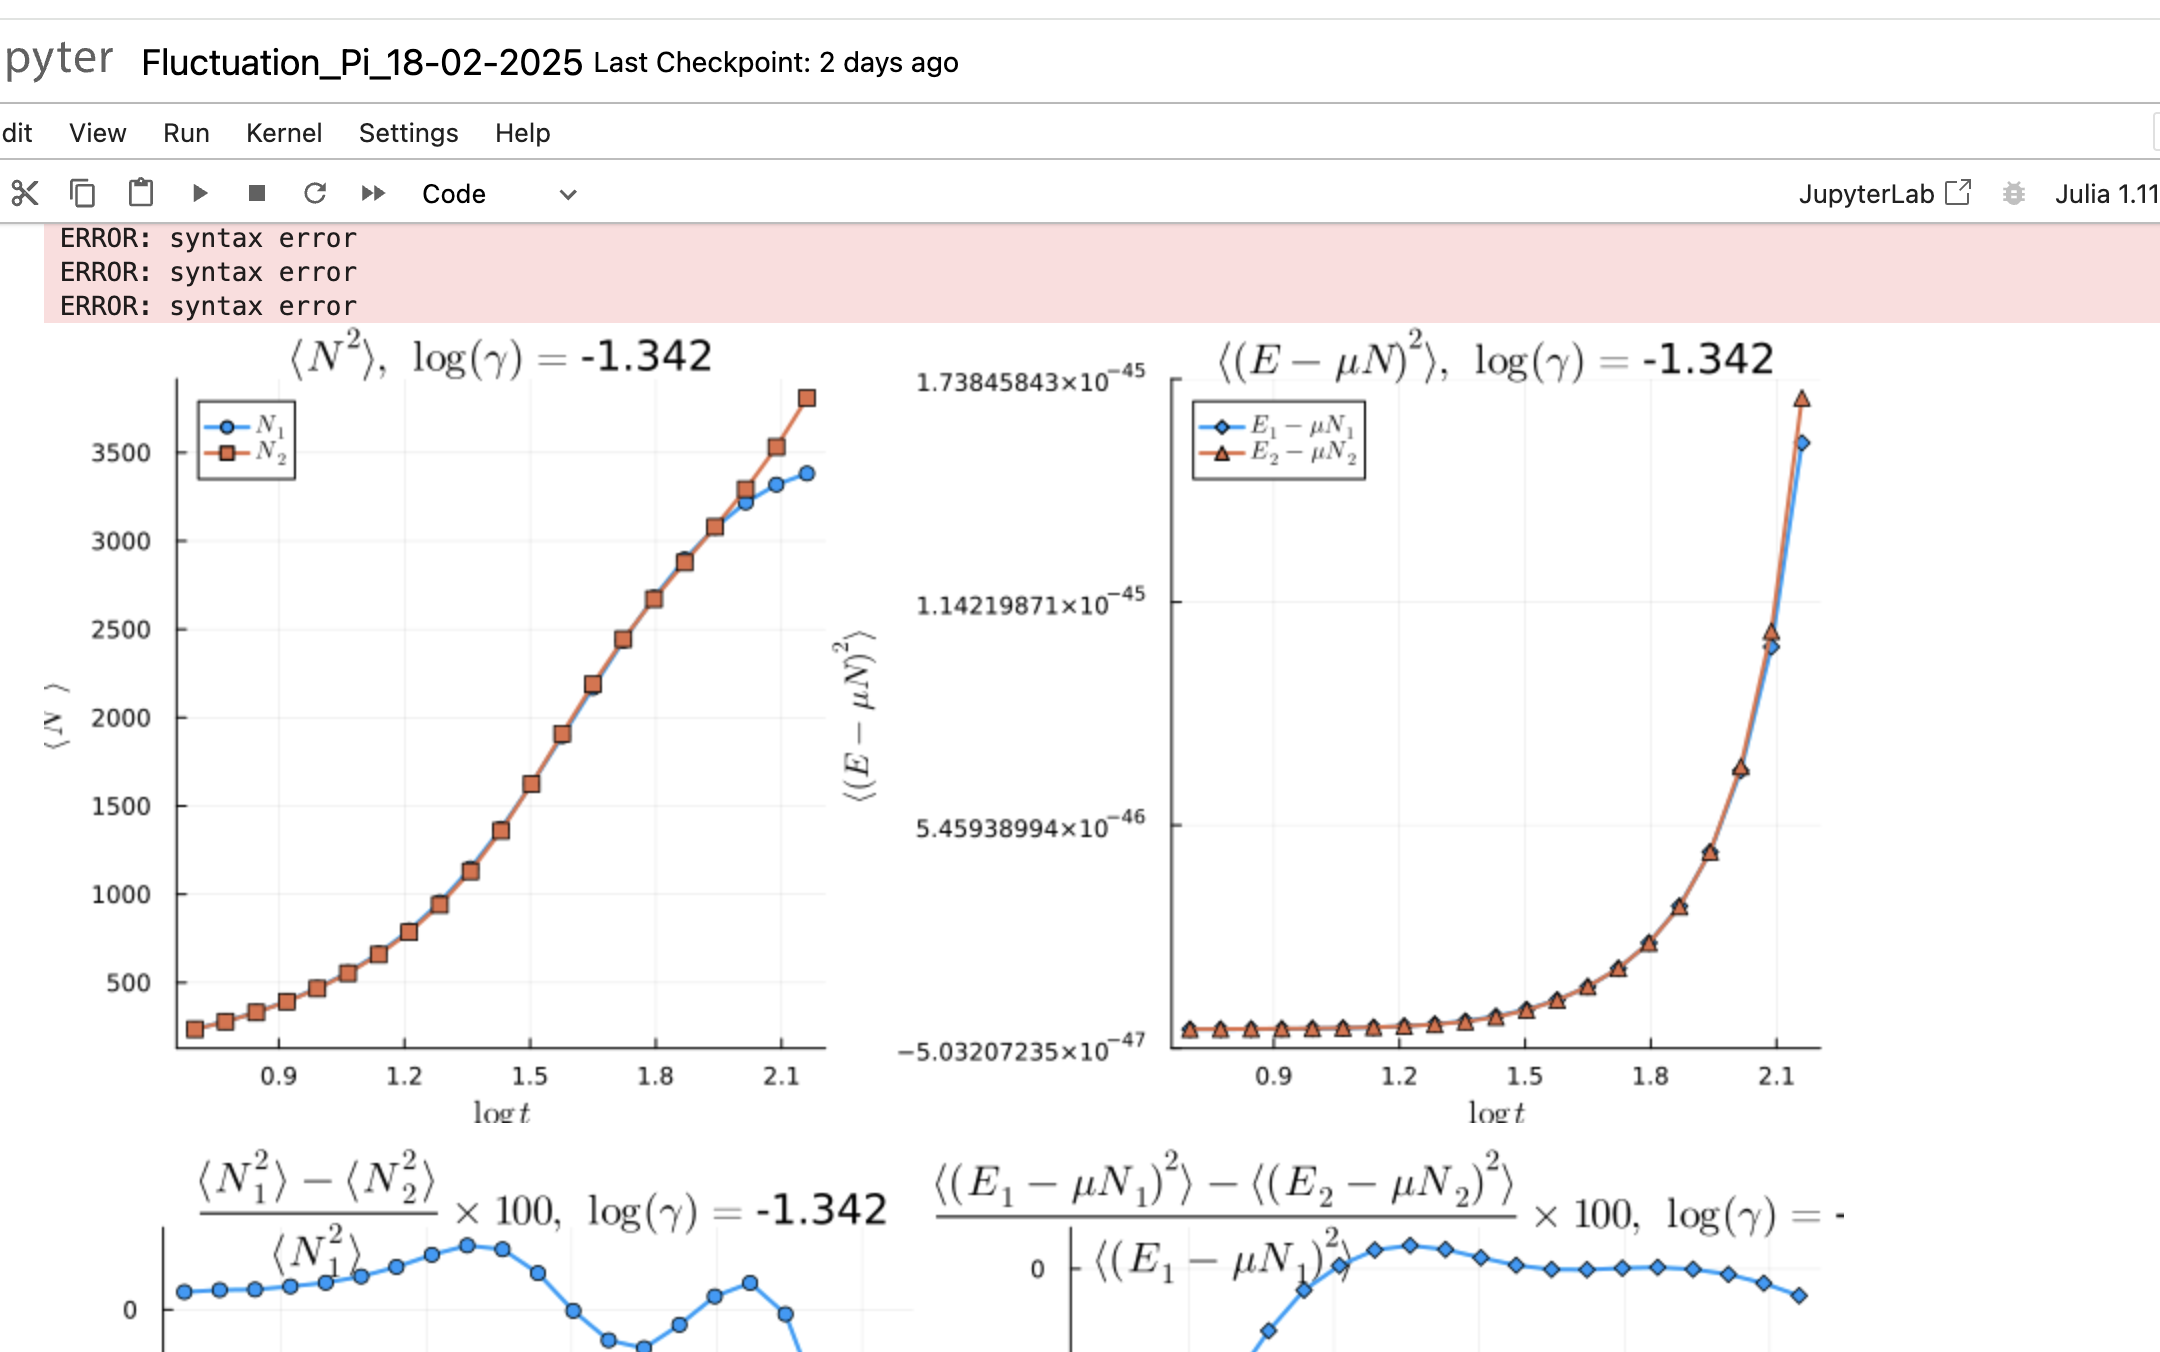
\includegraphics[width=1\textwidth]{Figures/test}

%\begin{aff}
%Donc une a l'ordre un en $\delta \theta (\operator{A}^{(0)})^{-1} %\operator{V}$ 

%\begin{eqnarray*}
%	\langle \delta \Pi ( \theta) \delta \Pi ( \theta') \rangle & = &  ( (\Pi^c_s - \Pi^c)\Pi^c/\Pi^c_s ) ( \theta ) \delta_{\theta, \theta'}/\delta \theta + \mathscr{F}(\theta , \theta' ) ,	
%\end{eqnarray*}

%avec 

%\begin{eqnarray*}
%	\mathscr{F}(\theta , \theta' ) & = & \left [ (\Pi^c_s - \Pi^c )( \theta)  +  (\Pi^c_s - \Pi^c ) ( \theta' )\right ] \frac{\Pi^c}{\Pi^c_s}(\theta)\frac{\Pi^c}{\Pi^c_s}(\theta') \frac{ \Delta( \theta'- \theta )}{ 2 \pi }\\
%	&&  - \left [ (\Pi^c_s - \Pi^c )( \theta)   (\Pi^c_s - \Pi^c ) ( \theta' )\right ] \frac{\Pi^c}{\Pi^c_s}(\theta)\frac{\Pi^c}{\Pi^c_s}(\theta')\int d\theta'' \left (   \frac{ \Pi^c/\Pi^c_s}{\Pi^c_s - \Pi^c} \right )(\theta'') \frac{\Delta(\theta''- \theta)}{2 \pi}\frac{\Delta(\theta''- \theta')}{2 \pi}  	
%\end{eqnarray*}
%\end{aff}



 









\subsection{Vérification explicite de la condition aux limites}
%Dans ce chapitre, nous nous intéressons aux fluctuations de la distribution de rapidité \( \delta \rho \) autour d'une distribution de référence \( \rho^c \), qui maximise la contribution à la fonction de partition des états, exprimée comme une fonctionnelle de la distribution \( \rho \) : 

La fonction de partition des états, s'exprime comme une fonctionnelle de la distribution \( \rho \) : 

\begin{eqnarray*}
	\Xi & = & \sum_\rho \exp \left( -\mathcal{A}(\rho) \right).
\end{eqnarray*}  

Dans la section {\em \bf Entropie de Yang-Yang} (\ref{??}), l'action \( \mathcal{A}(\rho) \) s'écrit sous la forme :  

\begin{eqnarray*}
	\mathcal{A}(\rho) & \doteq & - L\mathcal{S}_{YY}(\rho) + L\int f(\theta) \rho (\theta) \, d\theta,		
\end{eqnarray*}  

où \( \mathcal{S}_{YY} \) est la fonctionnelle d'entropie de Yang-Yang, définie dans (\ref{??}), et \( f \) est la fonction paramétrant les charges, introduite dans (\ref{??}).  

Dans cette même section {\em \bf Entropie de Yang-Yang} (\ref{??}), nous avons établi un lien entre \( f \) et distribution de référence \( \rho^c \), qui maximise la contribution à la fonction de partition des états .\\

On veux tester si nos experience est décrit pas un GGE. Pour cela nous nous intéressons aux fluctuations de la distribution de rapidité \( \delta \rho \) autour \( \rho^c \).

%Nous poursuivons à présent avec cette définition de l'action de classe $\mathcal{C}^2$ et admetant une distribution critique $\rho^c$ tel que sa différentielle en ce point critique soit nulle $d\mathcal{A}_{\rho^c} = 0 $ (\ref{??}) de sorte que d'aprés la formule de Taylor-Youg %afin de déterminer les fluctuations autour de \( \Pi^c \). Pour cela, nous réécrivons l'action sous la forme :  

Nous poursuivons à présent avec cette définition de l'action de classe $\mathcal{C}^2$ et admetant une distribution critique $\rho^c$ tel que sa différentielle en ce point critique soit nulle $d\mathcal{A}_{\rho^c} = 0 $ (\ref{??}) de sorte que d'aprés la formule de Taylor-Youg %afin de déterminer les fluctuations autour de \( \Pi^c \). Pour cela, nous réécrivons l'action sous la forme :  

\begin{eqnarray*}  
	\mathcal{A}(\rho^c + \delta \rho) & \underset{ \delta \rho \to 0 }{=} & \mathcal{A}(\rho^c)  + \frac{1}{2} \left. \frac{\delta^2 \mathcal{A}}{\delta \rho^2} \right|_{\rho^c} (\delta \rho) + \mathcal{O}((\delta \rho)^3),  
\end{eqnarray*}  

une expression quadratique pour l'action à l'ordre dominant en \( \delta \Pi \) avec $\left. \frac{\delta^2 \mathcal{A}}{\delta \rho^2} \right|_{\rho^c}$ la forme quadratique définie positive (Fig (\ref{fig.fluctu.A})).

\begin{figure}[H]
	\centering 
	\begin{tikzpicture}
		\begin{scope}[shift={(0,0)}]
			\begin{scope}[transform canvas={scale=0.6}]
				% Définition des couleurs avec les codes HTML
\definecolor{colorOne}{HTML}{443E46}
\definecolor{colorTwo}{HTML}{F6DEB8}
\definecolor{colorThree}{HTML}{908CA4}
\definecolor{colorFour}{HTML}{57659E}
\definecolor{colorFive}{HTML}{C57284}
\definecolor{colorSix}{HTML}{FF5B69}

% Raccourcis pour les couleurs
\def\colorOne{colorOne}
\def\colorTwo{colorTwo}
\def\colorThree{colorThree}
\def\colorFour{colorFour}
\def\colorFive{colorFive}
\def\colorSix{colorSix}

\def\colorslide{blue!50!black}



\begin{scope}
	% Tracer une courbe lisse entre des points
	\draw[shift={(0,0)} ,\colorOne]
		(-1 , 0 ) edge [thick,line width=0.8ex , ->,>=triangle 45  , \colorOne] node [pos = 1 , below ]{\huge$\rho$}( 5  , 0 )
	;
	\draw[shift={(0,0)}, color=\colorOne]
		(0, -1.0 ) edge [thick,line width=0.8ex , ->,>=triangle 45  ]node [pos=0.9,left=0.2cm ]{\huge$\mathcal{A}(\rho)$}( 0  , 5 )
	;
	\draw[]
		(2.5, 0.12 ) edge [thick,line width=0.8ex ,\colorThree ]node [pos=1,below  ]{\huge$\rho^c$} (2.5, -0.12 )	
	;
	
	\draw[]
		(2.5, -0.12 ) edge [thick,line width=0.4ex , dashed, \colorThree ] (2.5, 5.5 )
		(1.5, 1 ) edge [thick,line width=0.4ex , <->,>=triangle 45  , \colorThree ] (3.5, 1 )
		(-0.3,1) edge [thick,line width=0.4ex  , \colorThree ] node [pos=0,left ]{\huge$\mathcal{A}(\rho^c)$} (0.3, 1 )	
	;
    \draw[thick, line width=0.8ex , \colorFour] plot[smooth, tension=0.7] coordinates {
        (1, 5) (1.6 , 3 ) (2.5, 1) (3.5 , 3 )  (4, 5)
    };		
	
\end{scope}

	
			
			\end{scope}
			
			\draw[color = red , scale = 0.5 , draw = none  ] (-2 , -1) rectangle (5, 6) ; 	
		\end{scope}
		
		\begin{scope}[shift={(19,-1)}]
			\begin{scope}[transform canvas={scale=0.6}]
				% Définition des couleurs avec les codes HTML
\definecolor{colorOne}{HTML}{443E46}
\definecolor{colorTwo}{HTML}{F6DEB8}
\definecolor{colorThree}{HTML}{908CA4}
\definecolor{colorFour}{HTML}{57659E}
\definecolor{colorFive}{HTML}{C57284}
\definecolor{colorSix}{HTML}{FF5B69}

% Raccourcis pour les couleurs
\def\colorOne{colorOne}
\def\colorTwo{colorTwo}
\def\colorThree{colorThree}
\def\colorFour{colorFour}
\def\colorFive{colorFive}
\def\colorSix{colorSix}

\def\colorslide{blue!50!black}

\def\Occupation{
	\def\traitx{0.3}
	\def\traity{0.5}
	\draw[shift={(0,0)}]
		(-13.5 , 0 ) edge [thick,line width=0.8ex ]( -3.2  , 0 )
		( -3.2 - \traitx  , 0 - \traity ) edge [thick,line width=0.8ex ]( -3.2 + \traitx  , 0 + \traity  )
		( -2.8 - \traitx  , 0 - \traity ) edge [thick,line width=0.8ex ]( -2.8 + \traitx  , 0 + \traity  )
		(-2.8 , 0 ) edge [thick,line width=0.8ex ](2.8  , 0 )
		( 2.8 - \traitx  , 0 - \traity ) edge [thick,line width=0.8ex ]( 2.8 + \traitx  , 0 + \traity  )
		( 3.2 - \traitx  , 0 - \traity ) edge [thick,line width=0.8ex ]( 3.2 + \traitx  , 0 + \traity  )
		(3.2, 0 ) edge [thick,line width=0.8ex,->,>=triangle 45 , color = black ]node [pos=1.01,below  ]{\huge$\theta$}	( 13  , 0 )
	;
	\draw[shift={(0,0)}, color=\colorOne]
		(-10.5 , -1.5 ) edge [thick,line width=0.8ex , ->,>=triangle 45  ]( -10.5  , 4.5 )
	;
		
	\foreach \r in {1 , ... , 3 } {
%		\draw[
%		decoration={
%		markings,
%    	mark connection node=my node,
%    	mark=at position 0 with{\node [blue,transform shape] (my node) {\large \r};}},
%		color=gray, thick, 
%		line width=0.5ex] decorate { 
%            (-11.0, \r) -- (-10.1, \r )}
%        ;
        \draw[
			color=\colorOne,
			] 
            (-11.0, \r) edge[color=\colorThree , thick,line width=0.5ex] node [pos=-0.5 ]{\large\color{\colorFour} $\frac{\r}{\delta \theta}$ } (-10.3, \r )
        	;
	
	}
	

	
	% Graduation abcsisse 
	% Définitions des listes
% Definitions of the lists
\def\listetuple{-9/\theta_{1}, -8/\theta_{2} , -5/\theta_{3} , -2/\theta_{a-1} , 0/\theta_{a} , 1/\theta_{a+1} , 2/\theta_{a+2} ,  5/\theta_{N-4} , 7/\theta_{N-3},8/\theta_{N-1},9/\theta_{N} }
\def\listetrais{-12 , -11, -10, -9 , -8 , -7 ,  -6 , -5, -4.5,-4, -2 , -1, 0 , 0.5, 1, 2, 4 , 5 ,  6 , 7 , 8 ,8.5, 9 ,  10 , 11, 12 }

% Loop over listetrais
\foreach \r in \listetrais {
    % Initialize found variable to zero
    % Initialize found variable to zero
    %\pgfmathsetmacro\found{0}
    \global\def\found{0}
    \xdef\nomtheta{}
    
    % Check if \r is in listetuple
    \foreach \x/\y in \listetuple { 
        \ifdim \r pt=\x pt % If \r matches any \x in listetuple
            \global\def\found{1} ;
            \xdef\nomtheta{\y} % Set \nomtheta to the corresponding \y
            %\pgfmathsetmacro\found{1} % Set found to 1            
            %\global\pgfmathsetmacro\found{1}
        \fi
    }
    
    %\node [circle, draw, red] (A) at (\r, 2) {\found , $\nomtheta$};
    
    % Draw the line and display \nomtheta if found
    \ifnum\found=1
        \draw[color=\colorOne, thick, line width=0.5ex] 
            (\r, -0.3) -- (\r, 0.3) node[red , pos=-0.5] {\large $\nomtheta$};
         \filldraw[line width=0.5ex, color=\colorSix, outer color=\colorSix, inner color=\colorSix] 
            (\r, 0) circle (4pt);
    \else 
        % Draw without \nomtheta and add a blue circle if not found
        \draw[color=\colorOne, thick, line width=0.5ex] 
            (\r, -0.3) -- (\r, 0.3);
        \filldraw[line width=0.5ex, color=\colorSix, outer color=\colorTwo, inner color=\colorTwo] 
            (\r, 0) circle (4pt); 
    \fi
}

\def\listetrais{-9.5/\theta_{i-1}/2/3, -6.5/\theta_{i}/1/4  ,   -1.5/\theta_{j}/2/4 , 1.5/\theta_{j+1}/-1/3 , 3.5/\theta_{\ell-1}/1/3 , 6.5/\theta_{\ell}/3/4 , 9.5/\theta(\theta_{\ell+1})/-1/3 };



\foreach \r/\nomx/\y/\ys in \listetrais {
	\draw[
		decoration={
		markings,
    	mark connection node=my node,
    	mark=at position .5 with{\node [blue,transform shape] (my node) {\large \color{\colorFour} $\nomx$};}},
		color=\colorThree , thick, 
		line width=0.5ex] decorate { 
            (\r, 0.12) -- (\r, -1.2)}
        ;
     
     \ifdim \y pt > -1 pt 
     	\draw[
			decoration={
			markings,
    		mark connection node=my node,
    		mark=at position .5 with{\node [blue,transform shape] (my node) {\large \color{\colorFour} $\Pi(\nomx) $};}},
			color=\colorThree, thick, 
			line width=0.5ex] decorate { 
            (\r, \y) -- (\r +3, \y)}
        ;
        \draw[
			decoration={
			markings,
    		mark connection node=my node,
    		mark=at position .5 with{\node [blue,transform shape] (my node) {\large \color{\colorFive} $\Pi_s(\nomx) $};}},
			color=\colorFive, thick, 
			line width=0.5ex] decorate { 
            (\r, \ys) -- (\r +3, \ys)}
        ;
     \fi 
     \ifdim \r pt= -1.5 pt
     	\draw[
     		decoration={
			markings,
    		mark connection node=my node,
    		mark=at position .5 with{\node [blue,transform shape] (my node) {\large \color{\colorFour}  $\delta \theta $};},
    		%mark=at position 0.1  with {\arrow[blue, line width=0.5ex]{<}},
    		%mark=at position 1  with {\arrow[blue, line width=0.5ex]{>}}
    		},
        	color=\colorThree,
        	thick,
        	line width=0.5ex,
        	%arrows={Computer Modern Rightarrow[line cap=round]-Computer Modern Rightarrow[line cap=round]}
   			](\r, -1.2) edge[arrows={Computer Modern Rightarrow[line cap=round]-}] (\r + 0.4, -1.2)decorate {
    		(\r, -1.2) -- (\r + 3, -1.2)}(\r + 2, -1.2) edge[arrows={-Computer Modern Rightarrow[line cap=round]}] (\r + 3, -1.2)
    		;
    \fi
			
	
}


			
}


\begin{scope}
	%\draw[help lines , width=1.5ex] (-8,-3) grid (8,3);\draw[help lines ,width=0.5ex , opacity = 0.5] (-3,-3) grid[step=0.1] (3,3));
	
	%\draw[help lines] 
	%	(-3,-3) edge[width=1.5ex] grid (3,3)	
	%	(-3,-3) edge[width=0.5ex , opacity = 0.5] grid (3,3)	
	%;
	\begin{scope}[shift={(0,1)},rotate=0,opacity=1,color=black]
		\Occupation	
		
		%\node[anchor=east, font=\bfseries] at (-11, 0) {\color{red}\large (T = 0 )} ;	
	\end{scope}
	
	
	
	
	\begin{scope}[shift={(-10.5,7)},rotate=0,opacity=1,color=black]
	
	\begin{scope}[shift={(-0,0)},rotate=0,opacity=1,color=black]
	
		\draw[shift={(0,0)} ,line width=1ex,rounded corners = 1ex,color=\colorOne , opacity =1 ,fill=\colorOne!00 , pattern={north east lines} , pattern color=\colorOne!00 ]
			(0 , -1 ) rectangle (5,1)
		;
		

		\begin{scope}[shift={(0.5,0.5)}]
			\draw[color=\colorOne, thick, line width=0.5ex] 
            (0, -0.3) -- (0, 0.3) ;
            \filldraw[line width=0.5ex, color=\colorSix, outer color=\colorSix, inner color=\colorSix] 
            (0, 0) circle (4pt);
            
            \node[anchor=west, font=\bfseries] at (0.2, 0) {\color{\colorSix}\large : quasi-particule};
		\end{scope}
		
		\begin{scope}[shift={(0.5,-0.5)}]
			\draw[color=\colorOne, thick, line width=0.5ex] 
            (0, -0.3) -- (0, 0.3) ;
            \filldraw[line width=0.5ex, color=\colorSix, outer color=\colorTwo, inner color=\colorTwo] 
            (0, 0) circle (4pt);
            
            \node[anchor=west, font=\bfseries] at (0.2, 0) {\color{\colorSix}\large : hole};
		\end{scope}

	\end{scope}
	
	\begin{scope}[shift={(6,0)},rotate=0,opacity=1,color=black]	
		
		\draw[shift={(0,0)} ,line width=1ex,rounded corners = 1ex,color=\colorOne , opacity =1 ,fill=\colorOne!00 , pattern={north east lines} , pattern color=\colorOne!00 ]
			(0 , -1 ) rectangle (7.5,1)
		;
		
		\node[anchor=west] at (0.5, 0.5) {\color{\colorFour}\large $\Pi$ };\node[anchor=west, font=\bfseries] at (1, 0.5) {\color{\colorFour}\large : quasi-particule distribution};
		
		\node[anchor=west] at (0.5, -0.5) {\color{\colorFour}\large $\Pi_h$ };\node[anchor=west, font=\bfseries] at (1, -0.5) {\color{\colorFour}\large  : hole distribution};
		
	\end{scope}
	
	\begin{scope}[shift={(14.5,0)},rotate=0,opacity=1,color=black]	
		
		\draw[shift={(0,0)} ,line width=1ex,rounded corners = 1ex,color=\colorOne , opacity =1 ,fill=\colorOne!00 , pattern={north east lines} , pattern color=\colorOne!00 ]
			(0 , -0.5 ) rectangle (7.0,0.5)
		;
		
		\node[anchor=west] at (0.2, 0) {\color{\colorFour}\large ${\color{\colorFive}\Pi_s} = \Pi + \Pi_h $ } node[anchor=west , font=\bfseries] at (3.1 , 0 )  {\color{\colorFour}\large {\color{\colorFive} : density of states}};
		
	\end{scope}
	
	
	\end{scope}


		
	
\end{scope}

	
			
			\end{scope}
			\begin{scope}[scale=1]
				\draw[color = red , scale = 1 , draw = none  ] (-1 , -1) rectangle (5, 5) ; 
			\end{scope}	
		\end{scope}

		
				
			
	\end{tikzpicture}	
	\captionsetup{skip=10pt} % Ajoute de l’espace après la légende
	\label{fig.fluctu.A}
\end{figure}


On discrétise l'axe des rapidités en  petite cellule de rapidité $[\theta, \theta+\delta\theta]$, qui contient $L\rho(\theta) \delta \theta$ rapidités. 
	



Avec ces petites tranches, la forme quadratique s’écrit :

\begin{eqnarray*}
    \left. \frac{\delta^2 \mathcal{A}}{{\delta \rho}^2} \right|_{\rho^c}(\delta \rho ) &=&  \sum_{a,b \mid \text{tranche}}  
    \delta \rho(\theta_a)  \frac{\partial^2 \mathcal{A}}{\partial \delta \rho(\theta_a) \partial \delta \rho(\theta_b) } (\rho^c)  \delta \rho(\theta_b).
\end{eqnarray*}
Les fluctuations s’écrivent donc :

\begin{eqnarray*}
    \langle \delta \rho ( \theta) \delta \rho ( \theta') \rangle &=&  
    \frac{ \int d\delta \rho \, \delta \rho(\theta) \delta \rho ( \theta') 
    \exp \left( - \frac{1}{2} \sum_{a,b \mid \text{tranche}}  
    \delta \rho(\theta_a) \frac{\partial^2 \mathcal{A}}{\partial \delta \rho(\theta_a) \partial \delta \rho(\theta_b) } (\rho^c)  \delta \rho(\theta_b) \right) }
    { \int d\delta \Pi  
    \exp \left( - \frac{1}{2} \sum_{a,b \mid \text{tranche}}  
    \delta \rho(\theta_a) \frac{\partial^2 \mathcal{A}}{\partial \delta \rho(\theta_a) \partial \delta \rho(\theta_b) } (\rho^c)  \delta \rho(\theta_b) \right) } \\
    &=& \left( \mathbf{A}^{-1} \right)_{\theta , \theta'}
\end{eqnarray*}


\begin{aff}

\begin{eqnarray*}
	\langle \delta \rho ( \theta) \delta \rho ( \theta') \rangle &=& 	\left( \mathbf{A}^{-1} \right)_{\theta , \theta'}
\end{eqnarray*}

	
avec la  {\em matrice hessienne} $\mathbf{A}_{\theta , \theta'} \equiv \frac{\partial^2 \mathcal{A}}{\partial \delta \rho(\theta) \partial \delta \rho(\theta') }(\rho^c)$, au point critique/ qui maximise la probabilité  $\rho^c=\rho^c_s \nu^c $, s'écrit

\begin{eqnarray*}
	\operator{A} & = & \operator{A}^{(0)} + \delta \theta \operator{V}
\end{eqnarray*}

avec 

\begin{eqnarray*}
	A^{(0)}_{\theta , \theta'}  & = &  L\delta \theta \left ( \frac{ 1}{\rho^c_s ( 1  - \nu^c ) \nu^c } \right )(\theta)    \delta({\theta - \theta '})	,\\
	V_{\theta , \theta'}  &= & L \delta \theta \left \{ - \left [ \left ( \frac{1}{\rho^c_s( 1 - \nu^c) } \right ) ( \theta)  +  \left ( \frac{1}{\rho^c_s( 1 - \nu^c) } \right ) ( \theta' )\right ] \frac{ \Delta( \theta'- \theta )}{ 2 \pi } + \int d\theta''  \left ( \frac{\nu^c}{\rho^c_s( 1 - \nu^c) } \right )(\theta'') \frac{\Delta(\theta''- \theta)}{2 \pi}\frac{\Delta(\theta''- \theta')}{2 \pi}   \right \} 	
\end{eqnarray*}

\end{aff}

\subsection{Testes}

\begin{eqnarray*}
	\Delta_{\operator{\mathcal{N}}}^2  & = &  \frac{1}{\beta} \left . \frac{\partial \langle \operator{\mathcal{N}} \rangle}{\partial \mu} \right )_T \\
	\Delta_{\operator{\mathcal{E}}-\mu \operator{\mathcal{N}}}^2  & = &  - \left . \frac{\partial \langle \operator{\mathcal{E}}-\mu \operator{\mathcal{N}} \rangle}{\partial \beta} \right )_\mu 
\end{eqnarray*}

et 

\begin{eqnarray*}
	\Delta_{\operator{\mathcal{N}}}^2  &= & L^2 \int d\theta_a \int d \theta_b \, \langle \delta \rho(\theta_a) \delta \rho(\theta_b) \rangle \\
	\Delta_{\operator{\mathcal{E}}-\mu \operator{\mathcal{N}}}^2  & = & L^2 \int d\theta_a \int d \theta_b \, \left ( - \mu + \frac{1}2 m \theta_a^2  \right  )\left ( - \mu + \frac{1}2 m \theta_b^2  \right  )  \langle \delta \rho(\theta_a) \delta \rho(\theta_b) \rangle
\end{eqnarray*}

\includegraphics[width=1\textwidth]{Figures/test}

%\begin{aff}
%Donc une a l'ordre un en $\delta \theta (\operator{A}^{(0)})^{-1} %\operator{V}$ 

%\begin{eqnarray*}
%	\langle \delta \Pi ( \theta) \delta \Pi ( \theta') \rangle & = &  ( (\Pi^c_s - \Pi^c)\Pi^c/\Pi^c_s ) ( \theta ) \delta_{\theta, \theta'}/\delta \theta + \mathscr{F}(\theta , \theta' ) ,	
%\end{eqnarray*}

%avec 

%\begin{eqnarray*}
%	\mathscr{F}(\theta , \theta' ) & = & \left [ (\Pi^c_s - \Pi^c )( \theta)  +  (\Pi^c_s - \Pi^c ) ( \theta' )\right ] \frac{\Pi^c}{\Pi^c_s}(\theta)\frac{\Pi^c}{\Pi^c_s}(\theta') \frac{ \Delta( \theta'- \theta )}{ 2 \pi }\\
%	&&  - \left [ (\Pi^c_s - \Pi^c )( \theta)   (\Pi^c_s - \Pi^c ) ( \theta' )\right ] \frac{\Pi^c}{\Pi^c_s}(\theta)\frac{\Pi^c}{\Pi^c_s}(\theta')\int d\theta'' \left (   \frac{ \Pi^c/\Pi^c_s}{\Pi^c_s - \Pi^c} \right )(\theta'') \frac{\Delta(\theta''- \theta)}{2 \pi}\frac{\Delta(\theta''- \theta')}{2 \pi}  	
%\end{eqnarray*}
%\end{aff}



 











\subsection{Lien avec les équations de Bethe}
%Dans ce chapitre, nous nous intéressons aux fluctuations de la distribution de rapidité \( \delta \rho \) autour d'une distribution de référence \( \rho^c \), qui maximise la contribution à la fonction de partition des états, exprimée comme une fonctionnelle de la distribution \( \rho \) : 

La fonction de partition des états, s'exprime comme une fonctionnelle de la distribution \( \rho \) : 

\begin{eqnarray*}
	\Xi & = & \sum_\rho \exp \left( -\mathcal{A}(\rho) \right).
\end{eqnarray*}  

Dans la section {\em \bf Entropie de Yang-Yang} (\ref{??}), l'action \( \mathcal{A}(\rho) \) s'écrit sous la forme :  

\begin{eqnarray*}
	\mathcal{A}(\rho) & \doteq & - L\mathcal{S}_{YY}(\rho) + L\int f(\theta) \rho (\theta) \, d\theta,		
\end{eqnarray*}  

où \( \mathcal{S}_{YY} \) est la fonctionnelle d'entropie de Yang-Yang, définie dans (\ref{??}), et \( f \) est la fonction paramétrant les charges, introduite dans (\ref{??}).  

Dans cette même section {\em \bf Entropie de Yang-Yang} (\ref{??}), nous avons établi un lien entre \( f \) et distribution de référence \( \rho^c \), qui maximise la contribution à la fonction de partition des états .\\

On veux tester si nos experience est décrit pas un GGE. Pour cela nous nous intéressons aux fluctuations de la distribution de rapidité \( \delta \rho \) autour \( \rho^c \).

%Nous poursuivons à présent avec cette définition de l'action de classe $\mathcal{C}^2$ et admetant une distribution critique $\rho^c$ tel que sa différentielle en ce point critique soit nulle $d\mathcal{A}_{\rho^c} = 0 $ (\ref{??}) de sorte que d'aprés la formule de Taylor-Youg %afin de déterminer les fluctuations autour de \( \Pi^c \). Pour cela, nous réécrivons l'action sous la forme :  

Nous poursuivons à présent avec cette définition de l'action de classe $\mathcal{C}^2$ et admetant une distribution critique $\rho^c$ tel que sa différentielle en ce point critique soit nulle $d\mathcal{A}_{\rho^c} = 0 $ (\ref{??}) de sorte que d'aprés la formule de Taylor-Youg %afin de déterminer les fluctuations autour de \( \Pi^c \). Pour cela, nous réécrivons l'action sous la forme :  

\begin{eqnarray*}  
	\mathcal{A}(\rho^c + \delta \rho) & \underset{ \delta \rho \to 0 }{=} & \mathcal{A}(\rho^c)  + \frac{1}{2} \left. \frac{\delta^2 \mathcal{A}}{\delta \rho^2} \right|_{\rho^c} (\delta \rho) + \mathcal{O}((\delta \rho)^3),  
\end{eqnarray*}  

une expression quadratique pour l'action à l'ordre dominant en \( \delta \Pi \) avec $\left. \frac{\delta^2 \mathcal{A}}{\delta \rho^2} \right|_{\rho^c}$ la forme quadratique définie positive (Fig (\ref{fig.fluctu.A})).

\begin{figure}[H]
	\centering 
	\begin{tikzpicture}
		\begin{scope}[shift={(0,0)}]
			\begin{scope}[transform canvas={scale=0.6}]
				% Définition des couleurs avec les codes HTML
\definecolor{colorOne}{HTML}{443E46}
\definecolor{colorTwo}{HTML}{F6DEB8}
\definecolor{colorThree}{HTML}{908CA4}
\definecolor{colorFour}{HTML}{57659E}
\definecolor{colorFive}{HTML}{C57284}
\definecolor{colorSix}{HTML}{FF5B69}

% Raccourcis pour les couleurs
\def\colorOne{colorOne}
\def\colorTwo{colorTwo}
\def\colorThree{colorThree}
\def\colorFour{colorFour}
\def\colorFive{colorFive}
\def\colorSix{colorSix}

\def\colorslide{blue!50!black}



\begin{scope}
	% Tracer une courbe lisse entre des points
	\draw[shift={(0,0)} ,\colorOne]
		(-1 , 0 ) edge [thick,line width=0.8ex , ->,>=triangle 45  , \colorOne] node [pos = 1 , below ]{\huge$\rho$}( 5  , 0 )
	;
	\draw[shift={(0,0)}, color=\colorOne]
		(0, -1.0 ) edge [thick,line width=0.8ex , ->,>=triangle 45  ]node [pos=0.9,left=0.2cm ]{\huge$\mathcal{A}(\rho)$}( 0  , 5 )
	;
	\draw[]
		(2.5, 0.12 ) edge [thick,line width=0.8ex ,\colorThree ]node [pos=1,below  ]{\huge$\rho^c$} (2.5, -0.12 )	
	;
	
	\draw[]
		(2.5, -0.12 ) edge [thick,line width=0.4ex , dashed, \colorThree ] (2.5, 5.5 )
		(1.5, 1 ) edge [thick,line width=0.4ex , <->,>=triangle 45  , \colorThree ] (3.5, 1 )
		(-0.3,1) edge [thick,line width=0.4ex  , \colorThree ] node [pos=0,left ]{\huge$\mathcal{A}(\rho^c)$} (0.3, 1 )	
	;
    \draw[thick, line width=0.8ex , \colorFour] plot[smooth, tension=0.7] coordinates {
        (1, 5) (1.6 , 3 ) (2.5, 1) (3.5 , 3 )  (4, 5)
    };		
	
\end{scope}

	
			
			\end{scope}
			
			\draw[color = red , scale = 0.5 , draw = none  ] (-2 , -1) rectangle (5, 6) ; 	
		\end{scope}
		
		\begin{scope}[shift={(19,-1)}]
			\begin{scope}[transform canvas={scale=0.6}]
				% Définition des couleurs avec les codes HTML
\definecolor{colorOne}{HTML}{443E46}
\definecolor{colorTwo}{HTML}{F6DEB8}
\definecolor{colorThree}{HTML}{908CA4}
\definecolor{colorFour}{HTML}{57659E}
\definecolor{colorFive}{HTML}{C57284}
\definecolor{colorSix}{HTML}{FF5B69}

% Raccourcis pour les couleurs
\def\colorOne{colorOne}
\def\colorTwo{colorTwo}
\def\colorThree{colorThree}
\def\colorFour{colorFour}
\def\colorFive{colorFive}
\def\colorSix{colorSix}

\def\colorslide{blue!50!black}

\def\Occupation{
	\def\traitx{0.3}
	\def\traity{0.5}
	\draw[shift={(0,0)}]
		(-13.5 , 0 ) edge [thick,line width=0.8ex ]( -3.2  , 0 )
		( -3.2 - \traitx  , 0 - \traity ) edge [thick,line width=0.8ex ]( -3.2 + \traitx  , 0 + \traity  )
		( -2.8 - \traitx  , 0 - \traity ) edge [thick,line width=0.8ex ]( -2.8 + \traitx  , 0 + \traity  )
		(-2.8 , 0 ) edge [thick,line width=0.8ex ](2.8  , 0 )
		( 2.8 - \traitx  , 0 - \traity ) edge [thick,line width=0.8ex ]( 2.8 + \traitx  , 0 + \traity  )
		( 3.2 - \traitx  , 0 - \traity ) edge [thick,line width=0.8ex ]( 3.2 + \traitx  , 0 + \traity  )
		(3.2, 0 ) edge [thick,line width=0.8ex,->,>=triangle 45 , color = black ]node [pos=1.01,below  ]{\huge$\theta$}	( 13  , 0 )
	;
	\draw[shift={(0,0)}, color=\colorOne]
		(-10.5 , -1.5 ) edge [thick,line width=0.8ex , ->,>=triangle 45  ]( -10.5  , 4.5 )
	;
		
	\foreach \r in {1 , ... , 3 } {
%		\draw[
%		decoration={
%		markings,
%    	mark connection node=my node,
%    	mark=at position 0 with{\node [blue,transform shape] (my node) {\large \r};}},
%		color=gray, thick, 
%		line width=0.5ex] decorate { 
%            (-11.0, \r) -- (-10.1, \r )}
%        ;
        \draw[
			color=\colorOne,
			] 
            (-11.0, \r) edge[color=\colorThree , thick,line width=0.5ex] node [pos=-0.5 ]{\large\color{\colorFour} $\frac{\r}{\delta \theta}$ } (-10.3, \r )
        	;
	
	}
	

	
	% Graduation abcsisse 
	% Définitions des listes
% Definitions of the lists
\def\listetuple{-9/\theta_{1}, -8/\theta_{2} , -5/\theta_{3} , -2/\theta_{a-1} , 0/\theta_{a} , 1/\theta_{a+1} , 2/\theta_{a+2} ,  5/\theta_{N-4} , 7/\theta_{N-3},8/\theta_{N-1},9/\theta_{N} }
\def\listetrais{-12 , -11, -10, -9 , -8 , -7 ,  -6 , -5, -4.5,-4, -2 , -1, 0 , 0.5, 1, 2, 4 , 5 ,  6 , 7 , 8 ,8.5, 9 ,  10 , 11, 12 }

% Loop over listetrais
\foreach \r in \listetrais {
    % Initialize found variable to zero
    % Initialize found variable to zero
    %\pgfmathsetmacro\found{0}
    \global\def\found{0}
    \xdef\nomtheta{}
    
    % Check if \r is in listetuple
    \foreach \x/\y in \listetuple { 
        \ifdim \r pt=\x pt % If \r matches any \x in listetuple
            \global\def\found{1} ;
            \xdef\nomtheta{\y} % Set \nomtheta to the corresponding \y
            %\pgfmathsetmacro\found{1} % Set found to 1            
            %\global\pgfmathsetmacro\found{1}
        \fi
    }
    
    %\node [circle, draw, red] (A) at (\r, 2) {\found , $\nomtheta$};
    
    % Draw the line and display \nomtheta if found
    \ifnum\found=1
        \draw[color=\colorOne, thick, line width=0.5ex] 
            (\r, -0.3) -- (\r, 0.3) node[red , pos=-0.5] {\large $\nomtheta$};
         \filldraw[line width=0.5ex, color=\colorSix, outer color=\colorSix, inner color=\colorSix] 
            (\r, 0) circle (4pt);
    \else 
        % Draw without \nomtheta and add a blue circle if not found
        \draw[color=\colorOne, thick, line width=0.5ex] 
            (\r, -0.3) -- (\r, 0.3);
        \filldraw[line width=0.5ex, color=\colorSix, outer color=\colorTwo, inner color=\colorTwo] 
            (\r, 0) circle (4pt); 
    \fi
}

\def\listetrais{-9.5/\theta_{i-1}/2/3, -6.5/\theta_{i}/1/4  ,   -1.5/\theta_{j}/2/4 , 1.5/\theta_{j+1}/-1/3 , 3.5/\theta_{\ell-1}/1/3 , 6.5/\theta_{\ell}/3/4 , 9.5/\theta(\theta_{\ell+1})/-1/3 };



\foreach \r/\nomx/\y/\ys in \listetrais {
	\draw[
		decoration={
		markings,
    	mark connection node=my node,
    	mark=at position .5 with{\node [blue,transform shape] (my node) {\large \color{\colorFour} $\nomx$};}},
		color=\colorThree , thick, 
		line width=0.5ex] decorate { 
            (\r, 0.12) -- (\r, -1.2)}
        ;
     
     \ifdim \y pt > -1 pt 
     	\draw[
			decoration={
			markings,
    		mark connection node=my node,
    		mark=at position .5 with{\node [blue,transform shape] (my node) {\large \color{\colorFour} $\Pi(\nomx) $};}},
			color=\colorThree, thick, 
			line width=0.5ex] decorate { 
            (\r, \y) -- (\r +3, \y)}
        ;
        \draw[
			decoration={
			markings,
    		mark connection node=my node,
    		mark=at position .5 with{\node [blue,transform shape] (my node) {\large \color{\colorFive} $\Pi_s(\nomx) $};}},
			color=\colorFive, thick, 
			line width=0.5ex] decorate { 
            (\r, \ys) -- (\r +3, \ys)}
        ;
     \fi 
     \ifdim \r pt= -1.5 pt
     	\draw[
     		decoration={
			markings,
    		mark connection node=my node,
    		mark=at position .5 with{\node [blue,transform shape] (my node) {\large \color{\colorFour}  $\delta \theta $};},
    		%mark=at position 0.1  with {\arrow[blue, line width=0.5ex]{<}},
    		%mark=at position 1  with {\arrow[blue, line width=0.5ex]{>}}
    		},
        	color=\colorThree,
        	thick,
        	line width=0.5ex,
        	%arrows={Computer Modern Rightarrow[line cap=round]-Computer Modern Rightarrow[line cap=round]}
   			](\r, -1.2) edge[arrows={Computer Modern Rightarrow[line cap=round]-}] (\r + 0.4, -1.2)decorate {
    		(\r, -1.2) -- (\r + 3, -1.2)}(\r + 2, -1.2) edge[arrows={-Computer Modern Rightarrow[line cap=round]}] (\r + 3, -1.2)
    		;
    \fi
			
	
}


			
}


\begin{scope}
	%\draw[help lines , width=1.5ex] (-8,-3) grid (8,3);\draw[help lines ,width=0.5ex , opacity = 0.5] (-3,-3) grid[step=0.1] (3,3));
	
	%\draw[help lines] 
	%	(-3,-3) edge[width=1.5ex] grid (3,3)	
	%	(-3,-3) edge[width=0.5ex , opacity = 0.5] grid (3,3)	
	%;
	\begin{scope}[shift={(0,1)},rotate=0,opacity=1,color=black]
		\Occupation	
		
		%\node[anchor=east, font=\bfseries] at (-11, 0) {\color{red}\large (T = 0 )} ;	
	\end{scope}
	
	
	
	
	\begin{scope}[shift={(-10.5,7)},rotate=0,opacity=1,color=black]
	
	\begin{scope}[shift={(-0,0)},rotate=0,opacity=1,color=black]
	
		\draw[shift={(0,0)} ,line width=1ex,rounded corners = 1ex,color=\colorOne , opacity =1 ,fill=\colorOne!00 , pattern={north east lines} , pattern color=\colorOne!00 ]
			(0 , -1 ) rectangle (5,1)
		;
		

		\begin{scope}[shift={(0.5,0.5)}]
			\draw[color=\colorOne, thick, line width=0.5ex] 
            (0, -0.3) -- (0, 0.3) ;
            \filldraw[line width=0.5ex, color=\colorSix, outer color=\colorSix, inner color=\colorSix] 
            (0, 0) circle (4pt);
            
            \node[anchor=west, font=\bfseries] at (0.2, 0) {\color{\colorSix}\large : quasi-particule};
		\end{scope}
		
		\begin{scope}[shift={(0.5,-0.5)}]
			\draw[color=\colorOne, thick, line width=0.5ex] 
            (0, -0.3) -- (0, 0.3) ;
            \filldraw[line width=0.5ex, color=\colorSix, outer color=\colorTwo, inner color=\colorTwo] 
            (0, 0) circle (4pt);
            
            \node[anchor=west, font=\bfseries] at (0.2, 0) {\color{\colorSix}\large : hole};
		\end{scope}

	\end{scope}
	
	\begin{scope}[shift={(6,0)},rotate=0,opacity=1,color=black]	
		
		\draw[shift={(0,0)} ,line width=1ex,rounded corners = 1ex,color=\colorOne , opacity =1 ,fill=\colorOne!00 , pattern={north east lines} , pattern color=\colorOne!00 ]
			(0 , -1 ) rectangle (7.5,1)
		;
		
		\node[anchor=west] at (0.5, 0.5) {\color{\colorFour}\large $\Pi$ };\node[anchor=west, font=\bfseries] at (1, 0.5) {\color{\colorFour}\large : quasi-particule distribution};
		
		\node[anchor=west] at (0.5, -0.5) {\color{\colorFour}\large $\Pi_h$ };\node[anchor=west, font=\bfseries] at (1, -0.5) {\color{\colorFour}\large  : hole distribution};
		
	\end{scope}
	
	\begin{scope}[shift={(14.5,0)},rotate=0,opacity=1,color=black]	
		
		\draw[shift={(0,0)} ,line width=1ex,rounded corners = 1ex,color=\colorOne , opacity =1 ,fill=\colorOne!00 , pattern={north east lines} , pattern color=\colorOne!00 ]
			(0 , -0.5 ) rectangle (7.0,0.5)
		;
		
		\node[anchor=west] at (0.2, 0) {\color{\colorFour}\large ${\color{\colorFive}\Pi_s} = \Pi + \Pi_h $ } node[anchor=west , font=\bfseries] at (3.1 , 0 )  {\color{\colorFour}\large {\color{\colorFive} : density of states}};
		
	\end{scope}
	
	
	\end{scope}


		
	
\end{scope}

	
			
			\end{scope}
			\begin{scope}[scale=1]
				\draw[color = red , scale = 1 , draw = none  ] (-1 , -1) rectangle (5, 5) ; 
			\end{scope}	
		\end{scope}

		
				
			
	\end{tikzpicture}	
	\captionsetup{skip=10pt} % Ajoute de l’espace après la légende
	\label{fig.fluctu.A}
\end{figure}


On discrétise l'axe des rapidités en  petite cellule de rapidité $[\theta, \theta+\delta\theta]$, qui contient $L\rho(\theta) \delta \theta$ rapidités. 
	



Avec ces petites tranches, la forme quadratique s’écrit :

\begin{eqnarray*}
    \left. \frac{\delta^2 \mathcal{A}}{{\delta \rho}^2} \right|_{\rho^c}(\delta \rho ) &=&  \sum_{a,b \mid \text{tranche}}  
    \delta \rho(\theta_a)  \frac{\partial^2 \mathcal{A}}{\partial \delta \rho(\theta_a) \partial \delta \rho(\theta_b) } (\rho^c)  \delta \rho(\theta_b).
\end{eqnarray*}
Les fluctuations s’écrivent donc :

\begin{eqnarray*}
    \langle \delta \rho ( \theta) \delta \rho ( \theta') \rangle &=&  
    \frac{ \int d\delta \rho \, \delta \rho(\theta) \delta \rho ( \theta') 
    \exp \left( - \frac{1}{2} \sum_{a,b \mid \text{tranche}}  
    \delta \rho(\theta_a) \frac{\partial^2 \mathcal{A}}{\partial \delta \rho(\theta_a) \partial \delta \rho(\theta_b) } (\rho^c)  \delta \rho(\theta_b) \right) }
    { \int d\delta \Pi  
    \exp \left( - \frac{1}{2} \sum_{a,b \mid \text{tranche}}  
    \delta \rho(\theta_a) \frac{\partial^2 \mathcal{A}}{\partial \delta \rho(\theta_a) \partial \delta \rho(\theta_b) } (\rho^c)  \delta \rho(\theta_b) \right) } \\
    &=& \left( \mathbf{A}^{-1} \right)_{\theta , \theta'}
\end{eqnarray*}


\begin{aff}

\begin{eqnarray*}
	\langle \delta \rho ( \theta) \delta \rho ( \theta') \rangle &=& 	\left( \mathbf{A}^{-1} \right)_{\theta , \theta'}
\end{eqnarray*}

	
avec la  {\em matrice hessienne} $\mathbf{A}_{\theta , \theta'} \equiv \frac{\partial^2 \mathcal{A}}{\partial \delta \rho(\theta) \partial \delta \rho(\theta') }(\rho^c)$, au point critique/ qui maximise la probabilité  $\rho^c=\rho^c_s \nu^c $, s'écrit

\begin{eqnarray*}
	\operator{A} & = & \operator{A}^{(0)} + \delta \theta \operator{V}
\end{eqnarray*}

avec 

\begin{eqnarray*}
	A^{(0)}_{\theta , \theta'}  & = &  L\delta \theta \left ( \frac{ 1}{\rho^c_s ( 1  - \nu^c ) \nu^c } \right )(\theta)    \delta({\theta - \theta '})	,\\
	V_{\theta , \theta'}  &= & L \delta \theta \left \{ - \left [ \left ( \frac{1}{\rho^c_s( 1 - \nu^c) } \right ) ( \theta)  +  \left ( \frac{1}{\rho^c_s( 1 - \nu^c) } \right ) ( \theta' )\right ] \frac{ \Delta( \theta'- \theta )}{ 2 \pi } + \int d\theta''  \left ( \frac{\nu^c}{\rho^c_s( 1 - \nu^c) } \right )(\theta'') \frac{\Delta(\theta''- \theta)}{2 \pi}\frac{\Delta(\theta''- \theta')}{2 \pi}   \right \} 	
\end{eqnarray*}

\end{aff}

\subsection{Testes}

\begin{eqnarray*}
	\Delta_{\operator{\mathcal{N}}}^2  & = &  \frac{1}{\beta} \left . \frac{\partial \langle \operator{\mathcal{N}} \rangle}{\partial \mu} \right )_T \\
	\Delta_{\operator{\mathcal{E}}-\mu \operator{\mathcal{N}}}^2  & = &  - \left . \frac{\partial \langle \operator{\mathcal{E}}-\mu \operator{\mathcal{N}} \rangle}{\partial \beta} \right )_\mu 
\end{eqnarray*}

et 

\begin{eqnarray*}
	\Delta_{\operator{\mathcal{N}}}^2  &= & L^2 \int d\theta_a \int d \theta_b \, \langle \delta \rho(\theta_a) \delta \rho(\theta_b) \rangle \\
	\Delta_{\operator{\mathcal{E}}-\mu \operator{\mathcal{N}}}^2  & = & L^2 \int d\theta_a \int d \theta_b \, \left ( - \mu + \frac{1}2 m \theta_a^2  \right  )\left ( - \mu + \frac{1}2 m \theta_b^2  \right  )  \langle \delta \rho(\theta_a) \delta \rho(\theta_b) \rangle
\end{eqnarray*}

\includegraphics[width=1\textwidth]{Figures/test}

%\begin{aff}
%Donc une a l'ordre un en $\delta \theta (\operator{A}^{(0)})^{-1} %\operator{V}$ 

%\begin{eqnarray*}
%	\langle \delta \Pi ( \theta) \delta \Pi ( \theta') \rangle & = &  ( (\Pi^c_s - \Pi^c)\Pi^c/\Pi^c_s ) ( \theta ) \delta_{\theta, \theta'}/\delta \theta + \mathscr{F}(\theta , \theta' ) ,	
%\end{eqnarray*}

%avec 

%\begin{eqnarray*}
%	\mathscr{F}(\theta , \theta' ) & = & \left [ (\Pi^c_s - \Pi^c )( \theta)  +  (\Pi^c_s - \Pi^c ) ( \theta' )\right ] \frac{\Pi^c}{\Pi^c_s}(\theta)\frac{\Pi^c}{\Pi^c_s}(\theta') \frac{ \Delta( \theta'- \theta )}{ 2 \pi }\\
%	&&  - \left [ (\Pi^c_s - \Pi^c )( \theta)   (\Pi^c_s - \Pi^c ) ( \theta' )\right ] \frac{\Pi^c}{\Pi^c_s}(\theta)\frac{\Pi^c}{\Pi^c_s}(\theta')\int d\theta'' \left (   \frac{ \Pi^c/\Pi^c_s}{\Pi^c_s - \Pi^c} \right )(\theta'') \frac{\Delta(\theta''- \theta)}{2 \pi}\frac{\Delta(\theta''- \theta')}{2 \pi}  	
%\end{eqnarray*}
%\end{aff}



 













\subsection{Fonction d’onde et Hamiltonien et moment à 2 corps}
\subsection{Introduction au modèle de gaz de Bose unidimensionnel}
%Dans ce chapitre, nous nous intéressons aux fluctuations de la distribution de rapidité \( \delta \rho \) autour d'une distribution de référence \( \rho^c \), qui maximise la contribution à la fonction de partition des états, exprimée comme une fonctionnelle de la distribution \( \rho \) : 

La fonction de partition des états, s'exprime comme une fonctionnelle de la distribution \( \rho \) : 

\begin{eqnarray*}
	\Xi & = & \sum_\rho \exp \left( -\mathcal{A}(\rho) \right).
\end{eqnarray*}  

Dans la section {\em \bf Entropie de Yang-Yang} (\ref{??}), l'action \( \mathcal{A}(\rho) \) s'écrit sous la forme :  

\begin{eqnarray*}
	\mathcal{A}(\rho) & \doteq & - L\mathcal{S}_{YY}(\rho) + L\int f(\theta) \rho (\theta) \, d\theta,		
\end{eqnarray*}  

où \( \mathcal{S}_{YY} \) est la fonctionnelle d'entropie de Yang-Yang, définie dans (\ref{??}), et \( f \) est la fonction paramétrant les charges, introduite dans (\ref{??}).  

Dans cette même section {\em \bf Entropie de Yang-Yang} (\ref{??}), nous avons établi un lien entre \( f \) et distribution de référence \( \rho^c \), qui maximise la contribution à la fonction de partition des états .\\

On veux tester si nos experience est décrit pas un GGE. Pour cela nous nous intéressons aux fluctuations de la distribution de rapidité \( \delta \rho \) autour \( \rho^c \).

%Nous poursuivons à présent avec cette définition de l'action de classe $\mathcal{C}^2$ et admetant une distribution critique $\rho^c$ tel que sa différentielle en ce point critique soit nulle $d\mathcal{A}_{\rho^c} = 0 $ (\ref{??}) de sorte que d'aprés la formule de Taylor-Youg %afin de déterminer les fluctuations autour de \( \Pi^c \). Pour cela, nous réécrivons l'action sous la forme :  

Nous poursuivons à présent avec cette définition de l'action de classe $\mathcal{C}^2$ et admetant une distribution critique $\rho^c$ tel que sa différentielle en ce point critique soit nulle $d\mathcal{A}_{\rho^c} = 0 $ (\ref{??}) de sorte que d'aprés la formule de Taylor-Youg %afin de déterminer les fluctuations autour de \( \Pi^c \). Pour cela, nous réécrivons l'action sous la forme :  

\begin{eqnarray*}  
	\mathcal{A}(\rho^c + \delta \rho) & \underset{ \delta \rho \to 0 }{=} & \mathcal{A}(\rho^c)  + \frac{1}{2} \left. \frac{\delta^2 \mathcal{A}}{\delta \rho^2} \right|_{\rho^c} (\delta \rho) + \mathcal{O}((\delta \rho)^3),  
\end{eqnarray*}  

une expression quadratique pour l'action à l'ordre dominant en \( \delta \Pi \) avec $\left. \frac{\delta^2 \mathcal{A}}{\delta \rho^2} \right|_{\rho^c}$ la forme quadratique définie positive (Fig (\ref{fig.fluctu.A})).

\begin{figure}[H]
	\centering 
	\begin{tikzpicture}
		\begin{scope}[shift={(0,0)}]
			\begin{scope}[transform canvas={scale=0.6}]
				% Définition des couleurs avec les codes HTML
\definecolor{colorOne}{HTML}{443E46}
\definecolor{colorTwo}{HTML}{F6DEB8}
\definecolor{colorThree}{HTML}{908CA4}
\definecolor{colorFour}{HTML}{57659E}
\definecolor{colorFive}{HTML}{C57284}
\definecolor{colorSix}{HTML}{FF5B69}

% Raccourcis pour les couleurs
\def\colorOne{colorOne}
\def\colorTwo{colorTwo}
\def\colorThree{colorThree}
\def\colorFour{colorFour}
\def\colorFive{colorFive}
\def\colorSix{colorSix}

\def\colorslide{blue!50!black}



\begin{scope}
	% Tracer une courbe lisse entre des points
	\draw[shift={(0,0)} ,\colorOne]
		(-1 , 0 ) edge [thick,line width=0.8ex , ->,>=triangle 45  , \colorOne] node [pos = 1 , below ]{\huge$\rho$}( 5  , 0 )
	;
	\draw[shift={(0,0)}, color=\colorOne]
		(0, -1.0 ) edge [thick,line width=0.8ex , ->,>=triangle 45  ]node [pos=0.9,left=0.2cm ]{\huge$\mathcal{A}(\rho)$}( 0  , 5 )
	;
	\draw[]
		(2.5, 0.12 ) edge [thick,line width=0.8ex ,\colorThree ]node [pos=1,below  ]{\huge$\rho^c$} (2.5, -0.12 )	
	;
	
	\draw[]
		(2.5, -0.12 ) edge [thick,line width=0.4ex , dashed, \colorThree ] (2.5, 5.5 )
		(1.5, 1 ) edge [thick,line width=0.4ex , <->,>=triangle 45  , \colorThree ] (3.5, 1 )
		(-0.3,1) edge [thick,line width=0.4ex  , \colorThree ] node [pos=0,left ]{\huge$\mathcal{A}(\rho^c)$} (0.3, 1 )	
	;
    \draw[thick, line width=0.8ex , \colorFour] plot[smooth, tension=0.7] coordinates {
        (1, 5) (1.6 , 3 ) (2.5, 1) (3.5 , 3 )  (4, 5)
    };		
	
\end{scope}

	
			
			\end{scope}
			
			\draw[color = red , scale = 0.5 , draw = none  ] (-2 , -1) rectangle (5, 6) ; 	
		\end{scope}
		
		\begin{scope}[shift={(19,-1)}]
			\begin{scope}[transform canvas={scale=0.6}]
				% Définition des couleurs avec les codes HTML
\definecolor{colorOne}{HTML}{443E46}
\definecolor{colorTwo}{HTML}{F6DEB8}
\definecolor{colorThree}{HTML}{908CA4}
\definecolor{colorFour}{HTML}{57659E}
\definecolor{colorFive}{HTML}{C57284}
\definecolor{colorSix}{HTML}{FF5B69}

% Raccourcis pour les couleurs
\def\colorOne{colorOne}
\def\colorTwo{colorTwo}
\def\colorThree{colorThree}
\def\colorFour{colorFour}
\def\colorFive{colorFive}
\def\colorSix{colorSix}

\def\colorslide{blue!50!black}

\def\Occupation{
	\def\traitx{0.3}
	\def\traity{0.5}
	\draw[shift={(0,0)}]
		(-13.5 , 0 ) edge [thick,line width=0.8ex ]( -3.2  , 0 )
		( -3.2 - \traitx  , 0 - \traity ) edge [thick,line width=0.8ex ]( -3.2 + \traitx  , 0 + \traity  )
		( -2.8 - \traitx  , 0 - \traity ) edge [thick,line width=0.8ex ]( -2.8 + \traitx  , 0 + \traity  )
		(-2.8 , 0 ) edge [thick,line width=0.8ex ](2.8  , 0 )
		( 2.8 - \traitx  , 0 - \traity ) edge [thick,line width=0.8ex ]( 2.8 + \traitx  , 0 + \traity  )
		( 3.2 - \traitx  , 0 - \traity ) edge [thick,line width=0.8ex ]( 3.2 + \traitx  , 0 + \traity  )
		(3.2, 0 ) edge [thick,line width=0.8ex,->,>=triangle 45 , color = black ]node [pos=1.01,below  ]{\huge$\theta$}	( 13  , 0 )
	;
	\draw[shift={(0,0)}, color=\colorOne]
		(-10.5 , -1.5 ) edge [thick,line width=0.8ex , ->,>=triangle 45  ]( -10.5  , 4.5 )
	;
		
	\foreach \r in {1 , ... , 3 } {
%		\draw[
%		decoration={
%		markings,
%    	mark connection node=my node,
%    	mark=at position 0 with{\node [blue,transform shape] (my node) {\large \r};}},
%		color=gray, thick, 
%		line width=0.5ex] decorate { 
%            (-11.0, \r) -- (-10.1, \r )}
%        ;
        \draw[
			color=\colorOne,
			] 
            (-11.0, \r) edge[color=\colorThree , thick,line width=0.5ex] node [pos=-0.5 ]{\large\color{\colorFour} $\frac{\r}{\delta \theta}$ } (-10.3, \r )
        	;
	
	}
	

	
	% Graduation abcsisse 
	% Définitions des listes
% Definitions of the lists
\def\listetuple{-9/\theta_{1}, -8/\theta_{2} , -5/\theta_{3} , -2/\theta_{a-1} , 0/\theta_{a} , 1/\theta_{a+1} , 2/\theta_{a+2} ,  5/\theta_{N-4} , 7/\theta_{N-3},8/\theta_{N-1},9/\theta_{N} }
\def\listetrais{-12 , -11, -10, -9 , -8 , -7 ,  -6 , -5, -4.5,-4, -2 , -1, 0 , 0.5, 1, 2, 4 , 5 ,  6 , 7 , 8 ,8.5, 9 ,  10 , 11, 12 }

% Loop over listetrais
\foreach \r in \listetrais {
    % Initialize found variable to zero
    % Initialize found variable to zero
    %\pgfmathsetmacro\found{0}
    \global\def\found{0}
    \xdef\nomtheta{}
    
    % Check if \r is in listetuple
    \foreach \x/\y in \listetuple { 
        \ifdim \r pt=\x pt % If \r matches any \x in listetuple
            \global\def\found{1} ;
            \xdef\nomtheta{\y} % Set \nomtheta to the corresponding \y
            %\pgfmathsetmacro\found{1} % Set found to 1            
            %\global\pgfmathsetmacro\found{1}
        \fi
    }
    
    %\node [circle, draw, red] (A) at (\r, 2) {\found , $\nomtheta$};
    
    % Draw the line and display \nomtheta if found
    \ifnum\found=1
        \draw[color=\colorOne, thick, line width=0.5ex] 
            (\r, -0.3) -- (\r, 0.3) node[red , pos=-0.5] {\large $\nomtheta$};
         \filldraw[line width=0.5ex, color=\colorSix, outer color=\colorSix, inner color=\colorSix] 
            (\r, 0) circle (4pt);
    \else 
        % Draw without \nomtheta and add a blue circle if not found
        \draw[color=\colorOne, thick, line width=0.5ex] 
            (\r, -0.3) -- (\r, 0.3);
        \filldraw[line width=0.5ex, color=\colorSix, outer color=\colorTwo, inner color=\colorTwo] 
            (\r, 0) circle (4pt); 
    \fi
}

\def\listetrais{-9.5/\theta_{i-1}/2/3, -6.5/\theta_{i}/1/4  ,   -1.5/\theta_{j}/2/4 , 1.5/\theta_{j+1}/-1/3 , 3.5/\theta_{\ell-1}/1/3 , 6.5/\theta_{\ell}/3/4 , 9.5/\theta(\theta_{\ell+1})/-1/3 };



\foreach \r/\nomx/\y/\ys in \listetrais {
	\draw[
		decoration={
		markings,
    	mark connection node=my node,
    	mark=at position .5 with{\node [blue,transform shape] (my node) {\large \color{\colorFour} $\nomx$};}},
		color=\colorThree , thick, 
		line width=0.5ex] decorate { 
            (\r, 0.12) -- (\r, -1.2)}
        ;
     
     \ifdim \y pt > -1 pt 
     	\draw[
			decoration={
			markings,
    		mark connection node=my node,
    		mark=at position .5 with{\node [blue,transform shape] (my node) {\large \color{\colorFour} $\Pi(\nomx) $};}},
			color=\colorThree, thick, 
			line width=0.5ex] decorate { 
            (\r, \y) -- (\r +3, \y)}
        ;
        \draw[
			decoration={
			markings,
    		mark connection node=my node,
    		mark=at position .5 with{\node [blue,transform shape] (my node) {\large \color{\colorFive} $\Pi_s(\nomx) $};}},
			color=\colorFive, thick, 
			line width=0.5ex] decorate { 
            (\r, \ys) -- (\r +3, \ys)}
        ;
     \fi 
     \ifdim \r pt= -1.5 pt
     	\draw[
     		decoration={
			markings,
    		mark connection node=my node,
    		mark=at position .5 with{\node [blue,transform shape] (my node) {\large \color{\colorFour}  $\delta \theta $};},
    		%mark=at position 0.1  with {\arrow[blue, line width=0.5ex]{<}},
    		%mark=at position 1  with {\arrow[blue, line width=0.5ex]{>}}
    		},
        	color=\colorThree,
        	thick,
        	line width=0.5ex,
        	%arrows={Computer Modern Rightarrow[line cap=round]-Computer Modern Rightarrow[line cap=round]}
   			](\r, -1.2) edge[arrows={Computer Modern Rightarrow[line cap=round]-}] (\r + 0.4, -1.2)decorate {
    		(\r, -1.2) -- (\r + 3, -1.2)}(\r + 2, -1.2) edge[arrows={-Computer Modern Rightarrow[line cap=round]}] (\r + 3, -1.2)
    		;
    \fi
			
	
}


			
}


\begin{scope}
	%\draw[help lines , width=1.5ex] (-8,-3) grid (8,3);\draw[help lines ,width=0.5ex , opacity = 0.5] (-3,-3) grid[step=0.1] (3,3));
	
	%\draw[help lines] 
	%	(-3,-3) edge[width=1.5ex] grid (3,3)	
	%	(-3,-3) edge[width=0.5ex , opacity = 0.5] grid (3,3)	
	%;
	\begin{scope}[shift={(0,1)},rotate=0,opacity=1,color=black]
		\Occupation	
		
		%\node[anchor=east, font=\bfseries] at (-11, 0) {\color{red}\large (T = 0 )} ;	
	\end{scope}
	
	
	
	
	\begin{scope}[shift={(-10.5,7)},rotate=0,opacity=1,color=black]
	
	\begin{scope}[shift={(-0,0)},rotate=0,opacity=1,color=black]
	
		\draw[shift={(0,0)} ,line width=1ex,rounded corners = 1ex,color=\colorOne , opacity =1 ,fill=\colorOne!00 , pattern={north east lines} , pattern color=\colorOne!00 ]
			(0 , -1 ) rectangle (5,1)
		;
		

		\begin{scope}[shift={(0.5,0.5)}]
			\draw[color=\colorOne, thick, line width=0.5ex] 
            (0, -0.3) -- (0, 0.3) ;
            \filldraw[line width=0.5ex, color=\colorSix, outer color=\colorSix, inner color=\colorSix] 
            (0, 0) circle (4pt);
            
            \node[anchor=west, font=\bfseries] at (0.2, 0) {\color{\colorSix}\large : quasi-particule};
		\end{scope}
		
		\begin{scope}[shift={(0.5,-0.5)}]
			\draw[color=\colorOne, thick, line width=0.5ex] 
            (0, -0.3) -- (0, 0.3) ;
            \filldraw[line width=0.5ex, color=\colorSix, outer color=\colorTwo, inner color=\colorTwo] 
            (0, 0) circle (4pt);
            
            \node[anchor=west, font=\bfseries] at (0.2, 0) {\color{\colorSix}\large : hole};
		\end{scope}

	\end{scope}
	
	\begin{scope}[shift={(6,0)},rotate=0,opacity=1,color=black]	
		
		\draw[shift={(0,0)} ,line width=1ex,rounded corners = 1ex,color=\colorOne , opacity =1 ,fill=\colorOne!00 , pattern={north east lines} , pattern color=\colorOne!00 ]
			(0 , -1 ) rectangle (7.5,1)
		;
		
		\node[anchor=west] at (0.5, 0.5) {\color{\colorFour}\large $\Pi$ };\node[anchor=west, font=\bfseries] at (1, 0.5) {\color{\colorFour}\large : quasi-particule distribution};
		
		\node[anchor=west] at (0.5, -0.5) {\color{\colorFour}\large $\Pi_h$ };\node[anchor=west, font=\bfseries] at (1, -0.5) {\color{\colorFour}\large  : hole distribution};
		
	\end{scope}
	
	\begin{scope}[shift={(14.5,0)},rotate=0,opacity=1,color=black]	
		
		\draw[shift={(0,0)} ,line width=1ex,rounded corners = 1ex,color=\colorOne , opacity =1 ,fill=\colorOne!00 , pattern={north east lines} , pattern color=\colorOne!00 ]
			(0 , -0.5 ) rectangle (7.0,0.5)
		;
		
		\node[anchor=west] at (0.2, 0) {\color{\colorFour}\large ${\color{\colorFive}\Pi_s} = \Pi + \Pi_h $ } node[anchor=west , font=\bfseries] at (3.1 , 0 )  {\color{\colorFour}\large {\color{\colorFive} : density of states}};
		
	\end{scope}
	
	
	\end{scope}


		
	
\end{scope}

	
			
			\end{scope}
			\begin{scope}[scale=1]
				\draw[color = red , scale = 1 , draw = none  ] (-1 , -1) rectangle (5, 5) ; 
			\end{scope}	
		\end{scope}

		
				
			
	\end{tikzpicture}	
	\captionsetup{skip=10pt} % Ajoute de l’espace après la légende
	\label{fig.fluctu.A}
\end{figure}


On discrétise l'axe des rapidités en  petite cellule de rapidité $[\theta, \theta+\delta\theta]$, qui contient $L\rho(\theta) \delta \theta$ rapidités. 
	



Avec ces petites tranches, la forme quadratique s’écrit :

\begin{eqnarray*}
    \left. \frac{\delta^2 \mathcal{A}}{{\delta \rho}^2} \right|_{\rho^c}(\delta \rho ) &=&  \sum_{a,b \mid \text{tranche}}  
    \delta \rho(\theta_a)  \frac{\partial^2 \mathcal{A}}{\partial \delta \rho(\theta_a) \partial \delta \rho(\theta_b) } (\rho^c)  \delta \rho(\theta_b).
\end{eqnarray*}
Les fluctuations s’écrivent donc :

\begin{eqnarray*}
    \langle \delta \rho ( \theta) \delta \rho ( \theta') \rangle &=&  
    \frac{ \int d\delta \rho \, \delta \rho(\theta) \delta \rho ( \theta') 
    \exp \left( - \frac{1}{2} \sum_{a,b \mid \text{tranche}}  
    \delta \rho(\theta_a) \frac{\partial^2 \mathcal{A}}{\partial \delta \rho(\theta_a) \partial \delta \rho(\theta_b) } (\rho^c)  \delta \rho(\theta_b) \right) }
    { \int d\delta \Pi  
    \exp \left( - \frac{1}{2} \sum_{a,b \mid \text{tranche}}  
    \delta \rho(\theta_a) \frac{\partial^2 \mathcal{A}}{\partial \delta \rho(\theta_a) \partial \delta \rho(\theta_b) } (\rho^c)  \delta \rho(\theta_b) \right) } \\
    &=& \left( \mathbf{A}^{-1} \right)_{\theta , \theta'}
\end{eqnarray*}


\begin{aff}

\begin{eqnarray*}
	\langle \delta \rho ( \theta) \delta \rho ( \theta') \rangle &=& 	\left( \mathbf{A}^{-1} \right)_{\theta , \theta'}
\end{eqnarray*}

	
avec la  {\em matrice hessienne} $\mathbf{A}_{\theta , \theta'} \equiv \frac{\partial^2 \mathcal{A}}{\partial \delta \rho(\theta) \partial \delta \rho(\theta') }(\rho^c)$, au point critique/ qui maximise la probabilité  $\rho^c=\rho^c_s \nu^c $, s'écrit

\begin{eqnarray*}
	\operator{A} & = & \operator{A}^{(0)} + \delta \theta \operator{V}
\end{eqnarray*}

avec 

\begin{eqnarray*}
	A^{(0)}_{\theta , \theta'}  & = &  L\delta \theta \left ( \frac{ 1}{\rho^c_s ( 1  - \nu^c ) \nu^c } \right )(\theta)    \delta({\theta - \theta '})	,\\
	V_{\theta , \theta'}  &= & L \delta \theta \left \{ - \left [ \left ( \frac{1}{\rho^c_s( 1 - \nu^c) } \right ) ( \theta)  +  \left ( \frac{1}{\rho^c_s( 1 - \nu^c) } \right ) ( \theta' )\right ] \frac{ \Delta( \theta'- \theta )}{ 2 \pi } + \int d\theta''  \left ( \frac{\nu^c}{\rho^c_s( 1 - \nu^c) } \right )(\theta'') \frac{\Delta(\theta''- \theta)}{2 \pi}\frac{\Delta(\theta''- \theta')}{2 \pi}   \right \} 	
\end{eqnarray*}

\end{aff}

\subsection{Testes}

\begin{eqnarray*}
	\Delta_{\operator{\mathcal{N}}}^2  & = &  \frac{1}{\beta} \left . \frac{\partial \langle \operator{\mathcal{N}} \rangle}{\partial \mu} \right )_T \\
	\Delta_{\operator{\mathcal{E}}-\mu \operator{\mathcal{N}}}^2  & = &  - \left . \frac{\partial \langle \operator{\mathcal{E}}-\mu \operator{\mathcal{N}} \rangle}{\partial \beta} \right )_\mu 
\end{eqnarray*}

et 

\begin{eqnarray*}
	\Delta_{\operator{\mathcal{N}}}^2  &= & L^2 \int d\theta_a \int d \theta_b \, \langle \delta \rho(\theta_a) \delta \rho(\theta_b) \rangle \\
	\Delta_{\operator{\mathcal{E}}-\mu \operator{\mathcal{N}}}^2  & = & L^2 \int d\theta_a \int d \theta_b \, \left ( - \mu + \frac{1}2 m \theta_a^2  \right  )\left ( - \mu + \frac{1}2 m \theta_b^2  \right  )  \langle \delta \rho(\theta_a) \delta \rho(\theta_b) \rangle
\end{eqnarray*}

\includegraphics[width=1\textwidth]{Figures/test}

%\begin{aff}
%Donc une a l'ordre un en $\delta \theta (\operator{A}^{(0)})^{-1} %\operator{V}$ 

%\begin{eqnarray*}
%	\langle \delta \Pi ( \theta) \delta \Pi ( \theta') \rangle & = &  ( (\Pi^c_s - \Pi^c)\Pi^c/\Pi^c_s ) ( \theta ) \delta_{\theta, \theta'}/\delta \theta + \mathscr{F}(\theta , \theta' ) ,	
%\end{eqnarray*}

%avec 

%\begin{eqnarray*}
%	\mathscr{F}(\theta , \theta' ) & = & \left [ (\Pi^c_s - \Pi^c )( \theta)  +  (\Pi^c_s - \Pi^c ) ( \theta' )\right ] \frac{\Pi^c}{\Pi^c_s}(\theta)\frac{\Pi^c}{\Pi^c_s}(\theta') \frac{ \Delta( \theta'- \theta )}{ 2 \pi }\\
%	&&  - \left [ (\Pi^c_s - \Pi^c )( \theta)   (\Pi^c_s - \Pi^c ) ( \theta' )\right ] \frac{\Pi^c}{\Pi^c_s}(\theta)\frac{\Pi^c}{\Pi^c_s}(\theta')\int d\theta'' \left (   \frac{ \Pi^c/\Pi^c_s}{\Pi^c_s - \Pi^c} \right )(\theta'') \frac{\Delta(\theta''- \theta)}{2 \pi}\frac{\Delta(\theta''- \theta')}{2 \pi}  	
%\end{eqnarray*}
%\end{aff}



 









\subsection{Hamiltonien du modèle}
%Dans ce chapitre, nous nous intéressons aux fluctuations de la distribution de rapidité \( \delta \rho \) autour d'une distribution de référence \( \rho^c \), qui maximise la contribution à la fonction de partition des états, exprimée comme une fonctionnelle de la distribution \( \rho \) : 

La fonction de partition des états, s'exprime comme une fonctionnelle de la distribution \( \rho \) : 

\begin{eqnarray*}
	\Xi & = & \sum_\rho \exp \left( -\mathcal{A}(\rho) \right).
\end{eqnarray*}  

Dans la section {\em \bf Entropie de Yang-Yang} (\ref{??}), l'action \( \mathcal{A}(\rho) \) s'écrit sous la forme :  

\begin{eqnarray*}
	\mathcal{A}(\rho) & \doteq & - L\mathcal{S}_{YY}(\rho) + L\int f(\theta) \rho (\theta) \, d\theta,		
\end{eqnarray*}  

où \( \mathcal{S}_{YY} \) est la fonctionnelle d'entropie de Yang-Yang, définie dans (\ref{??}), et \( f \) est la fonction paramétrant les charges, introduite dans (\ref{??}).  

Dans cette même section {\em \bf Entropie de Yang-Yang} (\ref{??}), nous avons établi un lien entre \( f \) et distribution de référence \( \rho^c \), qui maximise la contribution à la fonction de partition des états .\\

On veux tester si nos experience est décrit pas un GGE. Pour cela nous nous intéressons aux fluctuations de la distribution de rapidité \( \delta \rho \) autour \( \rho^c \).

%Nous poursuivons à présent avec cette définition de l'action de classe $\mathcal{C}^2$ et admetant une distribution critique $\rho^c$ tel que sa différentielle en ce point critique soit nulle $d\mathcal{A}_{\rho^c} = 0 $ (\ref{??}) de sorte que d'aprés la formule de Taylor-Youg %afin de déterminer les fluctuations autour de \( \Pi^c \). Pour cela, nous réécrivons l'action sous la forme :  

Nous poursuivons à présent avec cette définition de l'action de classe $\mathcal{C}^2$ et admetant une distribution critique $\rho^c$ tel que sa différentielle en ce point critique soit nulle $d\mathcal{A}_{\rho^c} = 0 $ (\ref{??}) de sorte que d'aprés la formule de Taylor-Youg %afin de déterminer les fluctuations autour de \( \Pi^c \). Pour cela, nous réécrivons l'action sous la forme :  

\begin{eqnarray*}  
	\mathcal{A}(\rho^c + \delta \rho) & \underset{ \delta \rho \to 0 }{=} & \mathcal{A}(\rho^c)  + \frac{1}{2} \left. \frac{\delta^2 \mathcal{A}}{\delta \rho^2} \right|_{\rho^c} (\delta \rho) + \mathcal{O}((\delta \rho)^3),  
\end{eqnarray*}  

une expression quadratique pour l'action à l'ordre dominant en \( \delta \Pi \) avec $\left. \frac{\delta^2 \mathcal{A}}{\delta \rho^2} \right|_{\rho^c}$ la forme quadratique définie positive (Fig (\ref{fig.fluctu.A})).

\begin{figure}[H]
	\centering 
	\begin{tikzpicture}
		\begin{scope}[shift={(0,0)}]
			\begin{scope}[transform canvas={scale=0.6}]
				% Définition des couleurs avec les codes HTML
\definecolor{colorOne}{HTML}{443E46}
\definecolor{colorTwo}{HTML}{F6DEB8}
\definecolor{colorThree}{HTML}{908CA4}
\definecolor{colorFour}{HTML}{57659E}
\definecolor{colorFive}{HTML}{C57284}
\definecolor{colorSix}{HTML}{FF5B69}

% Raccourcis pour les couleurs
\def\colorOne{colorOne}
\def\colorTwo{colorTwo}
\def\colorThree{colorThree}
\def\colorFour{colorFour}
\def\colorFive{colorFive}
\def\colorSix{colorSix}

\def\colorslide{blue!50!black}



\begin{scope}
	% Tracer une courbe lisse entre des points
	\draw[shift={(0,0)} ,\colorOne]
		(-1 , 0 ) edge [thick,line width=0.8ex , ->,>=triangle 45  , \colorOne] node [pos = 1 , below ]{\huge$\rho$}( 5  , 0 )
	;
	\draw[shift={(0,0)}, color=\colorOne]
		(0, -1.0 ) edge [thick,line width=0.8ex , ->,>=triangle 45  ]node [pos=0.9,left=0.2cm ]{\huge$\mathcal{A}(\rho)$}( 0  , 5 )
	;
	\draw[]
		(2.5, 0.12 ) edge [thick,line width=0.8ex ,\colorThree ]node [pos=1,below  ]{\huge$\rho^c$} (2.5, -0.12 )	
	;
	
	\draw[]
		(2.5, -0.12 ) edge [thick,line width=0.4ex , dashed, \colorThree ] (2.5, 5.5 )
		(1.5, 1 ) edge [thick,line width=0.4ex , <->,>=triangle 45  , \colorThree ] (3.5, 1 )
		(-0.3,1) edge [thick,line width=0.4ex  , \colorThree ] node [pos=0,left ]{\huge$\mathcal{A}(\rho^c)$} (0.3, 1 )	
	;
    \draw[thick, line width=0.8ex , \colorFour] plot[smooth, tension=0.7] coordinates {
        (1, 5) (1.6 , 3 ) (2.5, 1) (3.5 , 3 )  (4, 5)
    };		
	
\end{scope}

	
			
			\end{scope}
			
			\draw[color = red , scale = 0.5 , draw = none  ] (-2 , -1) rectangle (5, 6) ; 	
		\end{scope}
		
		\begin{scope}[shift={(19,-1)}]
			\begin{scope}[transform canvas={scale=0.6}]
				% Définition des couleurs avec les codes HTML
\definecolor{colorOne}{HTML}{443E46}
\definecolor{colorTwo}{HTML}{F6DEB8}
\definecolor{colorThree}{HTML}{908CA4}
\definecolor{colorFour}{HTML}{57659E}
\definecolor{colorFive}{HTML}{C57284}
\definecolor{colorSix}{HTML}{FF5B69}

% Raccourcis pour les couleurs
\def\colorOne{colorOne}
\def\colorTwo{colorTwo}
\def\colorThree{colorThree}
\def\colorFour{colorFour}
\def\colorFive{colorFive}
\def\colorSix{colorSix}

\def\colorslide{blue!50!black}

\def\Occupation{
	\def\traitx{0.3}
	\def\traity{0.5}
	\draw[shift={(0,0)}]
		(-13.5 , 0 ) edge [thick,line width=0.8ex ]( -3.2  , 0 )
		( -3.2 - \traitx  , 0 - \traity ) edge [thick,line width=0.8ex ]( -3.2 + \traitx  , 0 + \traity  )
		( -2.8 - \traitx  , 0 - \traity ) edge [thick,line width=0.8ex ]( -2.8 + \traitx  , 0 + \traity  )
		(-2.8 , 0 ) edge [thick,line width=0.8ex ](2.8  , 0 )
		( 2.8 - \traitx  , 0 - \traity ) edge [thick,line width=0.8ex ]( 2.8 + \traitx  , 0 + \traity  )
		( 3.2 - \traitx  , 0 - \traity ) edge [thick,line width=0.8ex ]( 3.2 + \traitx  , 0 + \traity  )
		(3.2, 0 ) edge [thick,line width=0.8ex,->,>=triangle 45 , color = black ]node [pos=1.01,below  ]{\huge$\theta$}	( 13  , 0 )
	;
	\draw[shift={(0,0)}, color=\colorOne]
		(-10.5 , -1.5 ) edge [thick,line width=0.8ex , ->,>=triangle 45  ]( -10.5  , 4.5 )
	;
		
	\foreach \r in {1 , ... , 3 } {
%		\draw[
%		decoration={
%		markings,
%    	mark connection node=my node,
%    	mark=at position 0 with{\node [blue,transform shape] (my node) {\large \r};}},
%		color=gray, thick, 
%		line width=0.5ex] decorate { 
%            (-11.0, \r) -- (-10.1, \r )}
%        ;
        \draw[
			color=\colorOne,
			] 
            (-11.0, \r) edge[color=\colorThree , thick,line width=0.5ex] node [pos=-0.5 ]{\large\color{\colorFour} $\frac{\r}{\delta \theta}$ } (-10.3, \r )
        	;
	
	}
	

	
	% Graduation abcsisse 
	% Définitions des listes
% Definitions of the lists
\def\listetuple{-9/\theta_{1}, -8/\theta_{2} , -5/\theta_{3} , -2/\theta_{a-1} , 0/\theta_{a} , 1/\theta_{a+1} , 2/\theta_{a+2} ,  5/\theta_{N-4} , 7/\theta_{N-3},8/\theta_{N-1},9/\theta_{N} }
\def\listetrais{-12 , -11, -10, -9 , -8 , -7 ,  -6 , -5, -4.5,-4, -2 , -1, 0 , 0.5, 1, 2, 4 , 5 ,  6 , 7 , 8 ,8.5, 9 ,  10 , 11, 12 }

% Loop over listetrais
\foreach \r in \listetrais {
    % Initialize found variable to zero
    % Initialize found variable to zero
    %\pgfmathsetmacro\found{0}
    \global\def\found{0}
    \xdef\nomtheta{}
    
    % Check if \r is in listetuple
    \foreach \x/\y in \listetuple { 
        \ifdim \r pt=\x pt % If \r matches any \x in listetuple
            \global\def\found{1} ;
            \xdef\nomtheta{\y} % Set \nomtheta to the corresponding \y
            %\pgfmathsetmacro\found{1} % Set found to 1            
            %\global\pgfmathsetmacro\found{1}
        \fi
    }
    
    %\node [circle, draw, red] (A) at (\r, 2) {\found , $\nomtheta$};
    
    % Draw the line and display \nomtheta if found
    \ifnum\found=1
        \draw[color=\colorOne, thick, line width=0.5ex] 
            (\r, -0.3) -- (\r, 0.3) node[red , pos=-0.5] {\large $\nomtheta$};
         \filldraw[line width=0.5ex, color=\colorSix, outer color=\colorSix, inner color=\colorSix] 
            (\r, 0) circle (4pt);
    \else 
        % Draw without \nomtheta and add a blue circle if not found
        \draw[color=\colorOne, thick, line width=0.5ex] 
            (\r, -0.3) -- (\r, 0.3);
        \filldraw[line width=0.5ex, color=\colorSix, outer color=\colorTwo, inner color=\colorTwo] 
            (\r, 0) circle (4pt); 
    \fi
}

\def\listetrais{-9.5/\theta_{i-1}/2/3, -6.5/\theta_{i}/1/4  ,   -1.5/\theta_{j}/2/4 , 1.5/\theta_{j+1}/-1/3 , 3.5/\theta_{\ell-1}/1/3 , 6.5/\theta_{\ell}/3/4 , 9.5/\theta(\theta_{\ell+1})/-1/3 };



\foreach \r/\nomx/\y/\ys in \listetrais {
	\draw[
		decoration={
		markings,
    	mark connection node=my node,
    	mark=at position .5 with{\node [blue,transform shape] (my node) {\large \color{\colorFour} $\nomx$};}},
		color=\colorThree , thick, 
		line width=0.5ex] decorate { 
            (\r, 0.12) -- (\r, -1.2)}
        ;
     
     \ifdim \y pt > -1 pt 
     	\draw[
			decoration={
			markings,
    		mark connection node=my node,
    		mark=at position .5 with{\node [blue,transform shape] (my node) {\large \color{\colorFour} $\Pi(\nomx) $};}},
			color=\colorThree, thick, 
			line width=0.5ex] decorate { 
            (\r, \y) -- (\r +3, \y)}
        ;
        \draw[
			decoration={
			markings,
    		mark connection node=my node,
    		mark=at position .5 with{\node [blue,transform shape] (my node) {\large \color{\colorFive} $\Pi_s(\nomx) $};}},
			color=\colorFive, thick, 
			line width=0.5ex] decorate { 
            (\r, \ys) -- (\r +3, \ys)}
        ;
     \fi 
     \ifdim \r pt= -1.5 pt
     	\draw[
     		decoration={
			markings,
    		mark connection node=my node,
    		mark=at position .5 with{\node [blue,transform shape] (my node) {\large \color{\colorFour}  $\delta \theta $};},
    		%mark=at position 0.1  with {\arrow[blue, line width=0.5ex]{<}},
    		%mark=at position 1  with {\arrow[blue, line width=0.5ex]{>}}
    		},
        	color=\colorThree,
        	thick,
        	line width=0.5ex,
        	%arrows={Computer Modern Rightarrow[line cap=round]-Computer Modern Rightarrow[line cap=round]}
   			](\r, -1.2) edge[arrows={Computer Modern Rightarrow[line cap=round]-}] (\r + 0.4, -1.2)decorate {
    		(\r, -1.2) -- (\r + 3, -1.2)}(\r + 2, -1.2) edge[arrows={-Computer Modern Rightarrow[line cap=round]}] (\r + 3, -1.2)
    		;
    \fi
			
	
}


			
}


\begin{scope}
	%\draw[help lines , width=1.5ex] (-8,-3) grid (8,3);\draw[help lines ,width=0.5ex , opacity = 0.5] (-3,-3) grid[step=0.1] (3,3));
	
	%\draw[help lines] 
	%	(-3,-3) edge[width=1.5ex] grid (3,3)	
	%	(-3,-3) edge[width=0.5ex , opacity = 0.5] grid (3,3)	
	%;
	\begin{scope}[shift={(0,1)},rotate=0,opacity=1,color=black]
		\Occupation	
		
		%\node[anchor=east, font=\bfseries] at (-11, 0) {\color{red}\large (T = 0 )} ;	
	\end{scope}
	
	
	
	
	\begin{scope}[shift={(-10.5,7)},rotate=0,opacity=1,color=black]
	
	\begin{scope}[shift={(-0,0)},rotate=0,opacity=1,color=black]
	
		\draw[shift={(0,0)} ,line width=1ex,rounded corners = 1ex,color=\colorOne , opacity =1 ,fill=\colorOne!00 , pattern={north east lines} , pattern color=\colorOne!00 ]
			(0 , -1 ) rectangle (5,1)
		;
		

		\begin{scope}[shift={(0.5,0.5)}]
			\draw[color=\colorOne, thick, line width=0.5ex] 
            (0, -0.3) -- (0, 0.3) ;
            \filldraw[line width=0.5ex, color=\colorSix, outer color=\colorSix, inner color=\colorSix] 
            (0, 0) circle (4pt);
            
            \node[anchor=west, font=\bfseries] at (0.2, 0) {\color{\colorSix}\large : quasi-particule};
		\end{scope}
		
		\begin{scope}[shift={(0.5,-0.5)}]
			\draw[color=\colorOne, thick, line width=0.5ex] 
            (0, -0.3) -- (0, 0.3) ;
            \filldraw[line width=0.5ex, color=\colorSix, outer color=\colorTwo, inner color=\colorTwo] 
            (0, 0) circle (4pt);
            
            \node[anchor=west, font=\bfseries] at (0.2, 0) {\color{\colorSix}\large : hole};
		\end{scope}

	\end{scope}
	
	\begin{scope}[shift={(6,0)},rotate=0,opacity=1,color=black]	
		
		\draw[shift={(0,0)} ,line width=1ex,rounded corners = 1ex,color=\colorOne , opacity =1 ,fill=\colorOne!00 , pattern={north east lines} , pattern color=\colorOne!00 ]
			(0 , -1 ) rectangle (7.5,1)
		;
		
		\node[anchor=west] at (0.5, 0.5) {\color{\colorFour}\large $\Pi$ };\node[anchor=west, font=\bfseries] at (1, 0.5) {\color{\colorFour}\large : quasi-particule distribution};
		
		\node[anchor=west] at (0.5, -0.5) {\color{\colorFour}\large $\Pi_h$ };\node[anchor=west, font=\bfseries] at (1, -0.5) {\color{\colorFour}\large  : hole distribution};
		
	\end{scope}
	
	\begin{scope}[shift={(14.5,0)},rotate=0,opacity=1,color=black]	
		
		\draw[shift={(0,0)} ,line width=1ex,rounded corners = 1ex,color=\colorOne , opacity =1 ,fill=\colorOne!00 , pattern={north east lines} , pattern color=\colorOne!00 ]
			(0 , -0.5 ) rectangle (7.0,0.5)
		;
		
		\node[anchor=west] at (0.2, 0) {\color{\colorFour}\large ${\color{\colorFive}\Pi_s} = \Pi + \Pi_h $ } node[anchor=west , font=\bfseries] at (3.1 , 0 )  {\color{\colorFour}\large {\color{\colorFive} : density of states}};
		
	\end{scope}
	
	
	\end{scope}


		
	
\end{scope}

	
			
			\end{scope}
			\begin{scope}[scale=1]
				\draw[color = red , scale = 1 , draw = none  ] (-1 , -1) rectangle (5, 5) ; 
			\end{scope}	
		\end{scope}

		
				
			
	\end{tikzpicture}	
	\captionsetup{skip=10pt} % Ajoute de l’espace après la légende
	\label{fig.fluctu.A}
\end{figure}


On discrétise l'axe des rapidités en  petite cellule de rapidité $[\theta, \theta+\delta\theta]$, qui contient $L\rho(\theta) \delta \theta$ rapidités. 
	



Avec ces petites tranches, la forme quadratique s’écrit :

\begin{eqnarray*}
    \left. \frac{\delta^2 \mathcal{A}}{{\delta \rho}^2} \right|_{\rho^c}(\delta \rho ) &=&  \sum_{a,b \mid \text{tranche}}  
    \delta \rho(\theta_a)  \frac{\partial^2 \mathcal{A}}{\partial \delta \rho(\theta_a) \partial \delta \rho(\theta_b) } (\rho^c)  \delta \rho(\theta_b).
\end{eqnarray*}
Les fluctuations s’écrivent donc :

\begin{eqnarray*}
    \langle \delta \rho ( \theta) \delta \rho ( \theta') \rangle &=&  
    \frac{ \int d\delta \rho \, \delta \rho(\theta) \delta \rho ( \theta') 
    \exp \left( - \frac{1}{2} \sum_{a,b \mid \text{tranche}}  
    \delta \rho(\theta_a) \frac{\partial^2 \mathcal{A}}{\partial \delta \rho(\theta_a) \partial \delta \rho(\theta_b) } (\rho^c)  \delta \rho(\theta_b) \right) }
    { \int d\delta \Pi  
    \exp \left( - \frac{1}{2} \sum_{a,b \mid \text{tranche}}  
    \delta \rho(\theta_a) \frac{\partial^2 \mathcal{A}}{\partial \delta \rho(\theta_a) \partial \delta \rho(\theta_b) } (\rho^c)  \delta \rho(\theta_b) \right) } \\
    &=& \left( \mathbf{A}^{-1} \right)_{\theta , \theta'}
\end{eqnarray*}


\begin{aff}

\begin{eqnarray*}
	\langle \delta \rho ( \theta) \delta \rho ( \theta') \rangle &=& 	\left( \mathbf{A}^{-1} \right)_{\theta , \theta'}
\end{eqnarray*}

	
avec la  {\em matrice hessienne} $\mathbf{A}_{\theta , \theta'} \equiv \frac{\partial^2 \mathcal{A}}{\partial \delta \rho(\theta) \partial \delta \rho(\theta') }(\rho^c)$, au point critique/ qui maximise la probabilité  $\rho^c=\rho^c_s \nu^c $, s'écrit

\begin{eqnarray*}
	\operator{A} & = & \operator{A}^{(0)} + \delta \theta \operator{V}
\end{eqnarray*}

avec 

\begin{eqnarray*}
	A^{(0)}_{\theta , \theta'}  & = &  L\delta \theta \left ( \frac{ 1}{\rho^c_s ( 1  - \nu^c ) \nu^c } \right )(\theta)    \delta({\theta - \theta '})	,\\
	V_{\theta , \theta'}  &= & L \delta \theta \left \{ - \left [ \left ( \frac{1}{\rho^c_s( 1 - \nu^c) } \right ) ( \theta)  +  \left ( \frac{1}{\rho^c_s( 1 - \nu^c) } \right ) ( \theta' )\right ] \frac{ \Delta( \theta'- \theta )}{ 2 \pi } + \int d\theta''  \left ( \frac{\nu^c}{\rho^c_s( 1 - \nu^c) } \right )(\theta'') \frac{\Delta(\theta''- \theta)}{2 \pi}\frac{\Delta(\theta''- \theta')}{2 \pi}   \right \} 	
\end{eqnarray*}

\end{aff}

\subsection{Testes}

\begin{eqnarray*}
	\Delta_{\operator{\mathcal{N}}}^2  & = &  \frac{1}{\beta} \left . \frac{\partial \langle \operator{\mathcal{N}} \rangle}{\partial \mu} \right )_T \\
	\Delta_{\operator{\mathcal{E}}-\mu \operator{\mathcal{N}}}^2  & = &  - \left . \frac{\partial \langle \operator{\mathcal{E}}-\mu \operator{\mathcal{N}} \rangle}{\partial \beta} \right )_\mu 
\end{eqnarray*}

et 

\begin{eqnarray*}
	\Delta_{\operator{\mathcal{N}}}^2  &= & L^2 \int d\theta_a \int d \theta_b \, \langle \delta \rho(\theta_a) \delta \rho(\theta_b) \rangle \\
	\Delta_{\operator{\mathcal{E}}-\mu \operator{\mathcal{N}}}^2  & = & L^2 \int d\theta_a \int d \theta_b \, \left ( - \mu + \frac{1}2 m \theta_a^2  \right  )\left ( - \mu + \frac{1}2 m \theta_b^2  \right  )  \langle \delta \rho(\theta_a) \delta \rho(\theta_b) \rangle
\end{eqnarray*}

\includegraphics[width=1\textwidth]{Figures/test}

%\begin{aff}
%Donc une a l'ordre un en $\delta \theta (\operator{A}^{(0)})^{-1} %\operator{V}$ 

%\begin{eqnarray*}
%	\langle \delta \Pi ( \theta) \delta \Pi ( \theta') \rangle & = &  ( (\Pi^c_s - \Pi^c)\Pi^c/\Pi^c_s ) ( \theta ) \delta_{\theta, \theta'}/\delta \theta + \mathscr{F}(\theta , \theta' ) ,	
%\end{eqnarray*}

%avec 

%\begin{eqnarray*}
%	\mathscr{F}(\theta , \theta' ) & = & \left [ (\Pi^c_s - \Pi^c )( \theta)  +  (\Pi^c_s - \Pi^c ) ( \theta' )\right ] \frac{\Pi^c}{\Pi^c_s}(\theta)\frac{\Pi^c}{\Pi^c_s}(\theta') \frac{ \Delta( \theta'- \theta )}{ 2 \pi }\\
%	&&  - \left [ (\Pi^c_s - \Pi^c )( \theta)   (\Pi^c_s - \Pi^c ) ( \theta' )\right ] \frac{\Pi^c}{\Pi^c_s}(\theta)\frac{\Pi^c}{\Pi^c_s}(\theta')\int d\theta'' \left (   \frac{ \Pi^c/\Pi^c_s}{\Pi^c_s - \Pi^c} \right )(\theta'') \frac{\Delta(\theta''- \theta)}{2 \pi}\frac{\Delta(\theta''- \theta')}{2 \pi}  	
%\end{eqnarray*}
%\end{aff}



 









\subsection{États du vide et pseudovacuum}
%Dans ce chapitre, nous nous intéressons aux fluctuations de la distribution de rapidité \( \delta \rho \) autour d'une distribution de référence \( \rho^c \), qui maximise la contribution à la fonction de partition des états, exprimée comme une fonctionnelle de la distribution \( \rho \) : 

La fonction de partition des états, s'exprime comme une fonctionnelle de la distribution \( \rho \) : 

\begin{eqnarray*}
	\Xi & = & \sum_\rho \exp \left( -\mathcal{A}(\rho) \right).
\end{eqnarray*}  

Dans la section {\em \bf Entropie de Yang-Yang} (\ref{??}), l'action \( \mathcal{A}(\rho) \) s'écrit sous la forme :  

\begin{eqnarray*}
	\mathcal{A}(\rho) & \doteq & - L\mathcal{S}_{YY}(\rho) + L\int f(\theta) \rho (\theta) \, d\theta,		
\end{eqnarray*}  

où \( \mathcal{S}_{YY} \) est la fonctionnelle d'entropie de Yang-Yang, définie dans (\ref{??}), et \( f \) est la fonction paramétrant les charges, introduite dans (\ref{??}).  

Dans cette même section {\em \bf Entropie de Yang-Yang} (\ref{??}), nous avons établi un lien entre \( f \) et distribution de référence \( \rho^c \), qui maximise la contribution à la fonction de partition des états .\\

On veux tester si nos experience est décrit pas un GGE. Pour cela nous nous intéressons aux fluctuations de la distribution de rapidité \( \delta \rho \) autour \( \rho^c \).

%Nous poursuivons à présent avec cette définition de l'action de classe $\mathcal{C}^2$ et admetant une distribution critique $\rho^c$ tel que sa différentielle en ce point critique soit nulle $d\mathcal{A}_{\rho^c} = 0 $ (\ref{??}) de sorte que d'aprés la formule de Taylor-Youg %afin de déterminer les fluctuations autour de \( \Pi^c \). Pour cela, nous réécrivons l'action sous la forme :  

Nous poursuivons à présent avec cette définition de l'action de classe $\mathcal{C}^2$ et admetant une distribution critique $\rho^c$ tel que sa différentielle en ce point critique soit nulle $d\mathcal{A}_{\rho^c} = 0 $ (\ref{??}) de sorte que d'aprés la formule de Taylor-Youg %afin de déterminer les fluctuations autour de \( \Pi^c \). Pour cela, nous réécrivons l'action sous la forme :  

\begin{eqnarray*}  
	\mathcal{A}(\rho^c + \delta \rho) & \underset{ \delta \rho \to 0 }{=} & \mathcal{A}(\rho^c)  + \frac{1}{2} \left. \frac{\delta^2 \mathcal{A}}{\delta \rho^2} \right|_{\rho^c} (\delta \rho) + \mathcal{O}((\delta \rho)^3),  
\end{eqnarray*}  

une expression quadratique pour l'action à l'ordre dominant en \( \delta \Pi \) avec $\left. \frac{\delta^2 \mathcal{A}}{\delta \rho^2} \right|_{\rho^c}$ la forme quadratique définie positive (Fig (\ref{fig.fluctu.A})).

\begin{figure}[H]
	\centering 
	\begin{tikzpicture}
		\begin{scope}[shift={(0,0)}]
			\begin{scope}[transform canvas={scale=0.6}]
				% Définition des couleurs avec les codes HTML
\definecolor{colorOne}{HTML}{443E46}
\definecolor{colorTwo}{HTML}{F6DEB8}
\definecolor{colorThree}{HTML}{908CA4}
\definecolor{colorFour}{HTML}{57659E}
\definecolor{colorFive}{HTML}{C57284}
\definecolor{colorSix}{HTML}{FF5B69}

% Raccourcis pour les couleurs
\def\colorOne{colorOne}
\def\colorTwo{colorTwo}
\def\colorThree{colorThree}
\def\colorFour{colorFour}
\def\colorFive{colorFive}
\def\colorSix{colorSix}

\def\colorslide{blue!50!black}



\begin{scope}
	% Tracer une courbe lisse entre des points
	\draw[shift={(0,0)} ,\colorOne]
		(-1 , 0 ) edge [thick,line width=0.8ex , ->,>=triangle 45  , \colorOne] node [pos = 1 , below ]{\huge$\rho$}( 5  , 0 )
	;
	\draw[shift={(0,0)}, color=\colorOne]
		(0, -1.0 ) edge [thick,line width=0.8ex , ->,>=triangle 45  ]node [pos=0.9,left=0.2cm ]{\huge$\mathcal{A}(\rho)$}( 0  , 5 )
	;
	\draw[]
		(2.5, 0.12 ) edge [thick,line width=0.8ex ,\colorThree ]node [pos=1,below  ]{\huge$\rho^c$} (2.5, -0.12 )	
	;
	
	\draw[]
		(2.5, -0.12 ) edge [thick,line width=0.4ex , dashed, \colorThree ] (2.5, 5.5 )
		(1.5, 1 ) edge [thick,line width=0.4ex , <->,>=triangle 45  , \colorThree ] (3.5, 1 )
		(-0.3,1) edge [thick,line width=0.4ex  , \colorThree ] node [pos=0,left ]{\huge$\mathcal{A}(\rho^c)$} (0.3, 1 )	
	;
    \draw[thick, line width=0.8ex , \colorFour] plot[smooth, tension=0.7] coordinates {
        (1, 5) (1.6 , 3 ) (2.5, 1) (3.5 , 3 )  (4, 5)
    };		
	
\end{scope}

	
			
			\end{scope}
			
			\draw[color = red , scale = 0.5 , draw = none  ] (-2 , -1) rectangle (5, 6) ; 	
		\end{scope}
		
		\begin{scope}[shift={(19,-1)}]
			\begin{scope}[transform canvas={scale=0.6}]
				% Définition des couleurs avec les codes HTML
\definecolor{colorOne}{HTML}{443E46}
\definecolor{colorTwo}{HTML}{F6DEB8}
\definecolor{colorThree}{HTML}{908CA4}
\definecolor{colorFour}{HTML}{57659E}
\definecolor{colorFive}{HTML}{C57284}
\definecolor{colorSix}{HTML}{FF5B69}

% Raccourcis pour les couleurs
\def\colorOne{colorOne}
\def\colorTwo{colorTwo}
\def\colorThree{colorThree}
\def\colorFour{colorFour}
\def\colorFive{colorFive}
\def\colorSix{colorSix}

\def\colorslide{blue!50!black}

\def\Occupation{
	\def\traitx{0.3}
	\def\traity{0.5}
	\draw[shift={(0,0)}]
		(-13.5 , 0 ) edge [thick,line width=0.8ex ]( -3.2  , 0 )
		( -3.2 - \traitx  , 0 - \traity ) edge [thick,line width=0.8ex ]( -3.2 + \traitx  , 0 + \traity  )
		( -2.8 - \traitx  , 0 - \traity ) edge [thick,line width=0.8ex ]( -2.8 + \traitx  , 0 + \traity  )
		(-2.8 , 0 ) edge [thick,line width=0.8ex ](2.8  , 0 )
		( 2.8 - \traitx  , 0 - \traity ) edge [thick,line width=0.8ex ]( 2.8 + \traitx  , 0 + \traity  )
		( 3.2 - \traitx  , 0 - \traity ) edge [thick,line width=0.8ex ]( 3.2 + \traitx  , 0 + \traity  )
		(3.2, 0 ) edge [thick,line width=0.8ex,->,>=triangle 45 , color = black ]node [pos=1.01,below  ]{\huge$\theta$}	( 13  , 0 )
	;
	\draw[shift={(0,0)}, color=\colorOne]
		(-10.5 , -1.5 ) edge [thick,line width=0.8ex , ->,>=triangle 45  ]( -10.5  , 4.5 )
	;
		
	\foreach \r in {1 , ... , 3 } {
%		\draw[
%		decoration={
%		markings,
%    	mark connection node=my node,
%    	mark=at position 0 with{\node [blue,transform shape] (my node) {\large \r};}},
%		color=gray, thick, 
%		line width=0.5ex] decorate { 
%            (-11.0, \r) -- (-10.1, \r )}
%        ;
        \draw[
			color=\colorOne,
			] 
            (-11.0, \r) edge[color=\colorThree , thick,line width=0.5ex] node [pos=-0.5 ]{\large\color{\colorFour} $\frac{\r}{\delta \theta}$ } (-10.3, \r )
        	;
	
	}
	

	
	% Graduation abcsisse 
	% Définitions des listes
% Definitions of the lists
\def\listetuple{-9/\theta_{1}, -8/\theta_{2} , -5/\theta_{3} , -2/\theta_{a-1} , 0/\theta_{a} , 1/\theta_{a+1} , 2/\theta_{a+2} ,  5/\theta_{N-4} , 7/\theta_{N-3},8/\theta_{N-1},9/\theta_{N} }
\def\listetrais{-12 , -11, -10, -9 , -8 , -7 ,  -6 , -5, -4.5,-4, -2 , -1, 0 , 0.5, 1, 2, 4 , 5 ,  6 , 7 , 8 ,8.5, 9 ,  10 , 11, 12 }

% Loop over listetrais
\foreach \r in \listetrais {
    % Initialize found variable to zero
    % Initialize found variable to zero
    %\pgfmathsetmacro\found{0}
    \global\def\found{0}
    \xdef\nomtheta{}
    
    % Check if \r is in listetuple
    \foreach \x/\y in \listetuple { 
        \ifdim \r pt=\x pt % If \r matches any \x in listetuple
            \global\def\found{1} ;
            \xdef\nomtheta{\y} % Set \nomtheta to the corresponding \y
            %\pgfmathsetmacro\found{1} % Set found to 1            
            %\global\pgfmathsetmacro\found{1}
        \fi
    }
    
    %\node [circle, draw, red] (A) at (\r, 2) {\found , $\nomtheta$};
    
    % Draw the line and display \nomtheta if found
    \ifnum\found=1
        \draw[color=\colorOne, thick, line width=0.5ex] 
            (\r, -0.3) -- (\r, 0.3) node[red , pos=-0.5] {\large $\nomtheta$};
         \filldraw[line width=0.5ex, color=\colorSix, outer color=\colorSix, inner color=\colorSix] 
            (\r, 0) circle (4pt);
    \else 
        % Draw without \nomtheta and add a blue circle if not found
        \draw[color=\colorOne, thick, line width=0.5ex] 
            (\r, -0.3) -- (\r, 0.3);
        \filldraw[line width=0.5ex, color=\colorSix, outer color=\colorTwo, inner color=\colorTwo] 
            (\r, 0) circle (4pt); 
    \fi
}

\def\listetrais{-9.5/\theta_{i-1}/2/3, -6.5/\theta_{i}/1/4  ,   -1.5/\theta_{j}/2/4 , 1.5/\theta_{j+1}/-1/3 , 3.5/\theta_{\ell-1}/1/3 , 6.5/\theta_{\ell}/3/4 , 9.5/\theta(\theta_{\ell+1})/-1/3 };



\foreach \r/\nomx/\y/\ys in \listetrais {
	\draw[
		decoration={
		markings,
    	mark connection node=my node,
    	mark=at position .5 with{\node [blue,transform shape] (my node) {\large \color{\colorFour} $\nomx$};}},
		color=\colorThree , thick, 
		line width=0.5ex] decorate { 
            (\r, 0.12) -- (\r, -1.2)}
        ;
     
     \ifdim \y pt > -1 pt 
     	\draw[
			decoration={
			markings,
    		mark connection node=my node,
    		mark=at position .5 with{\node [blue,transform shape] (my node) {\large \color{\colorFour} $\Pi(\nomx) $};}},
			color=\colorThree, thick, 
			line width=0.5ex] decorate { 
            (\r, \y) -- (\r +3, \y)}
        ;
        \draw[
			decoration={
			markings,
    		mark connection node=my node,
    		mark=at position .5 with{\node [blue,transform shape] (my node) {\large \color{\colorFive} $\Pi_s(\nomx) $};}},
			color=\colorFive, thick, 
			line width=0.5ex] decorate { 
            (\r, \ys) -- (\r +3, \ys)}
        ;
     \fi 
     \ifdim \r pt= -1.5 pt
     	\draw[
     		decoration={
			markings,
    		mark connection node=my node,
    		mark=at position .5 with{\node [blue,transform shape] (my node) {\large \color{\colorFour}  $\delta \theta $};},
    		%mark=at position 0.1  with {\arrow[blue, line width=0.5ex]{<}},
    		%mark=at position 1  with {\arrow[blue, line width=0.5ex]{>}}
    		},
        	color=\colorThree,
        	thick,
        	line width=0.5ex,
        	%arrows={Computer Modern Rightarrow[line cap=round]-Computer Modern Rightarrow[line cap=round]}
   			](\r, -1.2) edge[arrows={Computer Modern Rightarrow[line cap=round]-}] (\r + 0.4, -1.2)decorate {
    		(\r, -1.2) -- (\r + 3, -1.2)}(\r + 2, -1.2) edge[arrows={-Computer Modern Rightarrow[line cap=round]}] (\r + 3, -1.2)
    		;
    \fi
			
	
}


			
}


\begin{scope}
	%\draw[help lines , width=1.5ex] (-8,-3) grid (8,3);\draw[help lines ,width=0.5ex , opacity = 0.5] (-3,-3) grid[step=0.1] (3,3));
	
	%\draw[help lines] 
	%	(-3,-3) edge[width=1.5ex] grid (3,3)	
	%	(-3,-3) edge[width=0.5ex , opacity = 0.5] grid (3,3)	
	%;
	\begin{scope}[shift={(0,1)},rotate=0,opacity=1,color=black]
		\Occupation	
		
		%\node[anchor=east, font=\bfseries] at (-11, 0) {\color{red}\large (T = 0 )} ;	
	\end{scope}
	
	
	
	
	\begin{scope}[shift={(-10.5,7)},rotate=0,opacity=1,color=black]
	
	\begin{scope}[shift={(-0,0)},rotate=0,opacity=1,color=black]
	
		\draw[shift={(0,0)} ,line width=1ex,rounded corners = 1ex,color=\colorOne , opacity =1 ,fill=\colorOne!00 , pattern={north east lines} , pattern color=\colorOne!00 ]
			(0 , -1 ) rectangle (5,1)
		;
		

		\begin{scope}[shift={(0.5,0.5)}]
			\draw[color=\colorOne, thick, line width=0.5ex] 
            (0, -0.3) -- (0, 0.3) ;
            \filldraw[line width=0.5ex, color=\colorSix, outer color=\colorSix, inner color=\colorSix] 
            (0, 0) circle (4pt);
            
            \node[anchor=west, font=\bfseries] at (0.2, 0) {\color{\colorSix}\large : quasi-particule};
		\end{scope}
		
		\begin{scope}[shift={(0.5,-0.5)}]
			\draw[color=\colorOne, thick, line width=0.5ex] 
            (0, -0.3) -- (0, 0.3) ;
            \filldraw[line width=0.5ex, color=\colorSix, outer color=\colorTwo, inner color=\colorTwo] 
            (0, 0) circle (4pt);
            
            \node[anchor=west, font=\bfseries] at (0.2, 0) {\color{\colorSix}\large : hole};
		\end{scope}

	\end{scope}
	
	\begin{scope}[shift={(6,0)},rotate=0,opacity=1,color=black]	
		
		\draw[shift={(0,0)} ,line width=1ex,rounded corners = 1ex,color=\colorOne , opacity =1 ,fill=\colorOne!00 , pattern={north east lines} , pattern color=\colorOne!00 ]
			(0 , -1 ) rectangle (7.5,1)
		;
		
		\node[anchor=west] at (0.5, 0.5) {\color{\colorFour}\large $\Pi$ };\node[anchor=west, font=\bfseries] at (1, 0.5) {\color{\colorFour}\large : quasi-particule distribution};
		
		\node[anchor=west] at (0.5, -0.5) {\color{\colorFour}\large $\Pi_h$ };\node[anchor=west, font=\bfseries] at (1, -0.5) {\color{\colorFour}\large  : hole distribution};
		
	\end{scope}
	
	\begin{scope}[shift={(14.5,0)},rotate=0,opacity=1,color=black]	
		
		\draw[shift={(0,0)} ,line width=1ex,rounded corners = 1ex,color=\colorOne , opacity =1 ,fill=\colorOne!00 , pattern={north east lines} , pattern color=\colorOne!00 ]
			(0 , -0.5 ) rectangle (7.0,0.5)
		;
		
		\node[anchor=west] at (0.2, 0) {\color{\colorFour}\large ${\color{\colorFive}\Pi_s} = \Pi + \Pi_h $ } node[anchor=west , font=\bfseries] at (3.1 , 0 )  {\color{\colorFour}\large {\color{\colorFive} : density of states}};
		
	\end{scope}
	
	
	\end{scope}


		
	
\end{scope}

	
			
			\end{scope}
			\begin{scope}[scale=1]
				\draw[color = red , scale = 1 , draw = none  ] (-1 , -1) rectangle (5, 5) ; 
			\end{scope}	
		\end{scope}

		
				
			
	\end{tikzpicture}	
	\captionsetup{skip=10pt} % Ajoute de l’espace après la légende
	\label{fig.fluctu.A}
\end{figure}


On discrétise l'axe des rapidités en  petite cellule de rapidité $[\theta, \theta+\delta\theta]$, qui contient $L\rho(\theta) \delta \theta$ rapidités. 
	



Avec ces petites tranches, la forme quadratique s’écrit :

\begin{eqnarray*}
    \left. \frac{\delta^2 \mathcal{A}}{{\delta \rho}^2} \right|_{\rho^c}(\delta \rho ) &=&  \sum_{a,b \mid \text{tranche}}  
    \delta \rho(\theta_a)  \frac{\partial^2 \mathcal{A}}{\partial \delta \rho(\theta_a) \partial \delta \rho(\theta_b) } (\rho^c)  \delta \rho(\theta_b).
\end{eqnarray*}
Les fluctuations s’écrivent donc :

\begin{eqnarray*}
    \langle \delta \rho ( \theta) \delta \rho ( \theta') \rangle &=&  
    \frac{ \int d\delta \rho \, \delta \rho(\theta) \delta \rho ( \theta') 
    \exp \left( - \frac{1}{2} \sum_{a,b \mid \text{tranche}}  
    \delta \rho(\theta_a) \frac{\partial^2 \mathcal{A}}{\partial \delta \rho(\theta_a) \partial \delta \rho(\theta_b) } (\rho^c)  \delta \rho(\theta_b) \right) }
    { \int d\delta \Pi  
    \exp \left( - \frac{1}{2} \sum_{a,b \mid \text{tranche}}  
    \delta \rho(\theta_a) \frac{\partial^2 \mathcal{A}}{\partial \delta \rho(\theta_a) \partial \delta \rho(\theta_b) } (\rho^c)  \delta \rho(\theta_b) \right) } \\
    &=& \left( \mathbf{A}^{-1} \right)_{\theta , \theta'}
\end{eqnarray*}


\begin{aff}

\begin{eqnarray*}
	\langle \delta \rho ( \theta) \delta \rho ( \theta') \rangle &=& 	\left( \mathbf{A}^{-1} \right)_{\theta , \theta'}
\end{eqnarray*}

	
avec la  {\em matrice hessienne} $\mathbf{A}_{\theta , \theta'} \equiv \frac{\partial^2 \mathcal{A}}{\partial \delta \rho(\theta) \partial \delta \rho(\theta') }(\rho^c)$, au point critique/ qui maximise la probabilité  $\rho^c=\rho^c_s \nu^c $, s'écrit

\begin{eqnarray*}
	\operator{A} & = & \operator{A}^{(0)} + \delta \theta \operator{V}
\end{eqnarray*}

avec 

\begin{eqnarray*}
	A^{(0)}_{\theta , \theta'}  & = &  L\delta \theta \left ( \frac{ 1}{\rho^c_s ( 1  - \nu^c ) \nu^c } \right )(\theta)    \delta({\theta - \theta '})	,\\
	V_{\theta , \theta'}  &= & L \delta \theta \left \{ - \left [ \left ( \frac{1}{\rho^c_s( 1 - \nu^c) } \right ) ( \theta)  +  \left ( \frac{1}{\rho^c_s( 1 - \nu^c) } \right ) ( \theta' )\right ] \frac{ \Delta( \theta'- \theta )}{ 2 \pi } + \int d\theta''  \left ( \frac{\nu^c}{\rho^c_s( 1 - \nu^c) } \right )(\theta'') \frac{\Delta(\theta''- \theta)}{2 \pi}\frac{\Delta(\theta''- \theta')}{2 \pi}   \right \} 	
\end{eqnarray*}

\end{aff}

\subsection{Testes}

\begin{eqnarray*}
	\Delta_{\operator{\mathcal{N}}}^2  & = &  \frac{1}{\beta} \left . \frac{\partial \langle \operator{\mathcal{N}} \rangle}{\partial \mu} \right )_T \\
	\Delta_{\operator{\mathcal{E}}-\mu \operator{\mathcal{N}}}^2  & = &  - \left . \frac{\partial \langle \operator{\mathcal{E}}-\mu \operator{\mathcal{N}} \rangle}{\partial \beta} \right )_\mu 
\end{eqnarray*}

et 

\begin{eqnarray*}
	\Delta_{\operator{\mathcal{N}}}^2  &= & L^2 \int d\theta_a \int d \theta_b \, \langle \delta \rho(\theta_a) \delta \rho(\theta_b) \rangle \\
	\Delta_{\operator{\mathcal{E}}-\mu \operator{\mathcal{N}}}^2  & = & L^2 \int d\theta_a \int d \theta_b \, \left ( - \mu + \frac{1}2 m \theta_a^2  \right  )\left ( - \mu + \frac{1}2 m \theta_b^2  \right  )  \langle \delta \rho(\theta_a) \delta \rho(\theta_b) \rangle
\end{eqnarray*}

\includegraphics[width=1\textwidth]{Figures/test}

%\begin{aff}
%Donc une a l'ordre un en $\delta \theta (\operator{A}^{(0)})^{-1} %\operator{V}$ 

%\begin{eqnarray*}
%	\langle \delta \Pi ( \theta) \delta \Pi ( \theta') \rangle & = &  ( (\Pi^c_s - \Pi^c)\Pi^c/\Pi^c_s ) ( \theta ) \delta_{\theta, \theta'}/\delta \theta + \mathscr{F}(\theta , \theta' ) ,	
%\end{eqnarray*}

%avec 

%\begin{eqnarray*}
%	\mathscr{F}(\theta , \theta' ) & = & \left [ (\Pi^c_s - \Pi^c )( \theta)  +  (\Pi^c_s - \Pi^c ) ( \theta' )\right ] \frac{\Pi^c}{\Pi^c_s}(\theta)\frac{\Pi^c}{\Pi^c_s}(\theta') \frac{ \Delta( \theta'- \theta )}{ 2 \pi }\\
%	&&  - \left [ (\Pi^c_s - \Pi^c )( \theta)   (\Pi^c_s - \Pi^c ) ( \theta' )\right ] \frac{\Pi^c}{\Pi^c_s}(\theta)\frac{\Pi^c}{\Pi^c_s}(\theta')\int d\theta'' \left (   \frac{ \Pi^c/\Pi^c_s}{\Pi^c_s - \Pi^c} \right )(\theta'') \frac{\Delta(\theta''- \theta)}{2 \pi}\frac{\Delta(\theta''- \theta')}{2 \pi}  	
%\end{eqnarray*}
%\end{aff}



 










\subsection{Opérateurs conservés (intégrales du mouvement)}
%Dans ce chapitre, nous nous intéressons aux fluctuations de la distribution de rapidité \( \delta \rho \) autour d'une distribution de référence \( \rho^c \), qui maximise la contribution à la fonction de partition des états, exprimée comme une fonctionnelle de la distribution \( \rho \) : 

La fonction de partition des états, s'exprime comme une fonctionnelle de la distribution \( \rho \) : 

\begin{eqnarray*}
	\Xi & = & \sum_\rho \exp \left( -\mathcal{A}(\rho) \right).
\end{eqnarray*}  

Dans la section {\em \bf Entropie de Yang-Yang} (\ref{??}), l'action \( \mathcal{A}(\rho) \) s'écrit sous la forme :  

\begin{eqnarray*}
	\mathcal{A}(\rho) & \doteq & - L\mathcal{S}_{YY}(\rho) + L\int f(\theta) \rho (\theta) \, d\theta,		
\end{eqnarray*}  

où \( \mathcal{S}_{YY} \) est la fonctionnelle d'entropie de Yang-Yang, définie dans (\ref{??}), et \( f \) est la fonction paramétrant les charges, introduite dans (\ref{??}).  

Dans cette même section {\em \bf Entropie de Yang-Yang} (\ref{??}), nous avons établi un lien entre \( f \) et distribution de référence \( \rho^c \), qui maximise la contribution à la fonction de partition des états .\\

On veux tester si nos experience est décrit pas un GGE. Pour cela nous nous intéressons aux fluctuations de la distribution de rapidité \( \delta \rho \) autour \( \rho^c \).

%Nous poursuivons à présent avec cette définition de l'action de classe $\mathcal{C}^2$ et admetant une distribution critique $\rho^c$ tel que sa différentielle en ce point critique soit nulle $d\mathcal{A}_{\rho^c} = 0 $ (\ref{??}) de sorte que d'aprés la formule de Taylor-Youg %afin de déterminer les fluctuations autour de \( \Pi^c \). Pour cela, nous réécrivons l'action sous la forme :  

Nous poursuivons à présent avec cette définition de l'action de classe $\mathcal{C}^2$ et admetant une distribution critique $\rho^c$ tel que sa différentielle en ce point critique soit nulle $d\mathcal{A}_{\rho^c} = 0 $ (\ref{??}) de sorte que d'aprés la formule de Taylor-Youg %afin de déterminer les fluctuations autour de \( \Pi^c \). Pour cela, nous réécrivons l'action sous la forme :  

\begin{eqnarray*}  
	\mathcal{A}(\rho^c + \delta \rho) & \underset{ \delta \rho \to 0 }{=} & \mathcal{A}(\rho^c)  + \frac{1}{2} \left. \frac{\delta^2 \mathcal{A}}{\delta \rho^2} \right|_{\rho^c} (\delta \rho) + \mathcal{O}((\delta \rho)^3),  
\end{eqnarray*}  

une expression quadratique pour l'action à l'ordre dominant en \( \delta \Pi \) avec $\left. \frac{\delta^2 \mathcal{A}}{\delta \rho^2} \right|_{\rho^c}$ la forme quadratique définie positive (Fig (\ref{fig.fluctu.A})).

\begin{figure}[H]
	\centering 
	\begin{tikzpicture}
		\begin{scope}[shift={(0,0)}]
			\begin{scope}[transform canvas={scale=0.6}]
				% Définition des couleurs avec les codes HTML
\definecolor{colorOne}{HTML}{443E46}
\definecolor{colorTwo}{HTML}{F6DEB8}
\definecolor{colorThree}{HTML}{908CA4}
\definecolor{colorFour}{HTML}{57659E}
\definecolor{colorFive}{HTML}{C57284}
\definecolor{colorSix}{HTML}{FF5B69}

% Raccourcis pour les couleurs
\def\colorOne{colorOne}
\def\colorTwo{colorTwo}
\def\colorThree{colorThree}
\def\colorFour{colorFour}
\def\colorFive{colorFive}
\def\colorSix{colorSix}

\def\colorslide{blue!50!black}



\begin{scope}
	% Tracer une courbe lisse entre des points
	\draw[shift={(0,0)} ,\colorOne]
		(-1 , 0 ) edge [thick,line width=0.8ex , ->,>=triangle 45  , \colorOne] node [pos = 1 , below ]{\huge$\rho$}( 5  , 0 )
	;
	\draw[shift={(0,0)}, color=\colorOne]
		(0, -1.0 ) edge [thick,line width=0.8ex , ->,>=triangle 45  ]node [pos=0.9,left=0.2cm ]{\huge$\mathcal{A}(\rho)$}( 0  , 5 )
	;
	\draw[]
		(2.5, 0.12 ) edge [thick,line width=0.8ex ,\colorThree ]node [pos=1,below  ]{\huge$\rho^c$} (2.5, -0.12 )	
	;
	
	\draw[]
		(2.5, -0.12 ) edge [thick,line width=0.4ex , dashed, \colorThree ] (2.5, 5.5 )
		(1.5, 1 ) edge [thick,line width=0.4ex , <->,>=triangle 45  , \colorThree ] (3.5, 1 )
		(-0.3,1) edge [thick,line width=0.4ex  , \colorThree ] node [pos=0,left ]{\huge$\mathcal{A}(\rho^c)$} (0.3, 1 )	
	;
    \draw[thick, line width=0.8ex , \colorFour] plot[smooth, tension=0.7] coordinates {
        (1, 5) (1.6 , 3 ) (2.5, 1) (3.5 , 3 )  (4, 5)
    };		
	
\end{scope}

	
			
			\end{scope}
			
			\draw[color = red , scale = 0.5 , draw = none  ] (-2 , -1) rectangle (5, 6) ; 	
		\end{scope}
		
		\begin{scope}[shift={(19,-1)}]
			\begin{scope}[transform canvas={scale=0.6}]
				% Définition des couleurs avec les codes HTML
\definecolor{colorOne}{HTML}{443E46}
\definecolor{colorTwo}{HTML}{F6DEB8}
\definecolor{colorThree}{HTML}{908CA4}
\definecolor{colorFour}{HTML}{57659E}
\definecolor{colorFive}{HTML}{C57284}
\definecolor{colorSix}{HTML}{FF5B69}

% Raccourcis pour les couleurs
\def\colorOne{colorOne}
\def\colorTwo{colorTwo}
\def\colorThree{colorThree}
\def\colorFour{colorFour}
\def\colorFive{colorFive}
\def\colorSix{colorSix}

\def\colorslide{blue!50!black}

\def\Occupation{
	\def\traitx{0.3}
	\def\traity{0.5}
	\draw[shift={(0,0)}]
		(-13.5 , 0 ) edge [thick,line width=0.8ex ]( -3.2  , 0 )
		( -3.2 - \traitx  , 0 - \traity ) edge [thick,line width=0.8ex ]( -3.2 + \traitx  , 0 + \traity  )
		( -2.8 - \traitx  , 0 - \traity ) edge [thick,line width=0.8ex ]( -2.8 + \traitx  , 0 + \traity  )
		(-2.8 , 0 ) edge [thick,line width=0.8ex ](2.8  , 0 )
		( 2.8 - \traitx  , 0 - \traity ) edge [thick,line width=0.8ex ]( 2.8 + \traitx  , 0 + \traity  )
		( 3.2 - \traitx  , 0 - \traity ) edge [thick,line width=0.8ex ]( 3.2 + \traitx  , 0 + \traity  )
		(3.2, 0 ) edge [thick,line width=0.8ex,->,>=triangle 45 , color = black ]node [pos=1.01,below  ]{\huge$\theta$}	( 13  , 0 )
	;
	\draw[shift={(0,0)}, color=\colorOne]
		(-10.5 , -1.5 ) edge [thick,line width=0.8ex , ->,>=triangle 45  ]( -10.5  , 4.5 )
	;
		
	\foreach \r in {1 , ... , 3 } {
%		\draw[
%		decoration={
%		markings,
%    	mark connection node=my node,
%    	mark=at position 0 with{\node [blue,transform shape] (my node) {\large \r};}},
%		color=gray, thick, 
%		line width=0.5ex] decorate { 
%            (-11.0, \r) -- (-10.1, \r )}
%        ;
        \draw[
			color=\colorOne,
			] 
            (-11.0, \r) edge[color=\colorThree , thick,line width=0.5ex] node [pos=-0.5 ]{\large\color{\colorFour} $\frac{\r}{\delta \theta}$ } (-10.3, \r )
        	;
	
	}
	

	
	% Graduation abcsisse 
	% Définitions des listes
% Definitions of the lists
\def\listetuple{-9/\theta_{1}, -8/\theta_{2} , -5/\theta_{3} , -2/\theta_{a-1} , 0/\theta_{a} , 1/\theta_{a+1} , 2/\theta_{a+2} ,  5/\theta_{N-4} , 7/\theta_{N-3},8/\theta_{N-1},9/\theta_{N} }
\def\listetrais{-12 , -11, -10, -9 , -8 , -7 ,  -6 , -5, -4.5,-4, -2 , -1, 0 , 0.5, 1, 2, 4 , 5 ,  6 , 7 , 8 ,8.5, 9 ,  10 , 11, 12 }

% Loop over listetrais
\foreach \r in \listetrais {
    % Initialize found variable to zero
    % Initialize found variable to zero
    %\pgfmathsetmacro\found{0}
    \global\def\found{0}
    \xdef\nomtheta{}
    
    % Check if \r is in listetuple
    \foreach \x/\y in \listetuple { 
        \ifdim \r pt=\x pt % If \r matches any \x in listetuple
            \global\def\found{1} ;
            \xdef\nomtheta{\y} % Set \nomtheta to the corresponding \y
            %\pgfmathsetmacro\found{1} % Set found to 1            
            %\global\pgfmathsetmacro\found{1}
        \fi
    }
    
    %\node [circle, draw, red] (A) at (\r, 2) {\found , $\nomtheta$};
    
    % Draw the line and display \nomtheta if found
    \ifnum\found=1
        \draw[color=\colorOne, thick, line width=0.5ex] 
            (\r, -0.3) -- (\r, 0.3) node[red , pos=-0.5] {\large $\nomtheta$};
         \filldraw[line width=0.5ex, color=\colorSix, outer color=\colorSix, inner color=\colorSix] 
            (\r, 0) circle (4pt);
    \else 
        % Draw without \nomtheta and add a blue circle if not found
        \draw[color=\colorOne, thick, line width=0.5ex] 
            (\r, -0.3) -- (\r, 0.3);
        \filldraw[line width=0.5ex, color=\colorSix, outer color=\colorTwo, inner color=\colorTwo] 
            (\r, 0) circle (4pt); 
    \fi
}

\def\listetrais{-9.5/\theta_{i-1}/2/3, -6.5/\theta_{i}/1/4  ,   -1.5/\theta_{j}/2/4 , 1.5/\theta_{j+1}/-1/3 , 3.5/\theta_{\ell-1}/1/3 , 6.5/\theta_{\ell}/3/4 , 9.5/\theta(\theta_{\ell+1})/-1/3 };



\foreach \r/\nomx/\y/\ys in \listetrais {
	\draw[
		decoration={
		markings,
    	mark connection node=my node,
    	mark=at position .5 with{\node [blue,transform shape] (my node) {\large \color{\colorFour} $\nomx$};}},
		color=\colorThree , thick, 
		line width=0.5ex] decorate { 
            (\r, 0.12) -- (\r, -1.2)}
        ;
     
     \ifdim \y pt > -1 pt 
     	\draw[
			decoration={
			markings,
    		mark connection node=my node,
    		mark=at position .5 with{\node [blue,transform shape] (my node) {\large \color{\colorFour} $\Pi(\nomx) $};}},
			color=\colorThree, thick, 
			line width=0.5ex] decorate { 
            (\r, \y) -- (\r +3, \y)}
        ;
        \draw[
			decoration={
			markings,
    		mark connection node=my node,
    		mark=at position .5 with{\node [blue,transform shape] (my node) {\large \color{\colorFive} $\Pi_s(\nomx) $};}},
			color=\colorFive, thick, 
			line width=0.5ex] decorate { 
            (\r, \ys) -- (\r +3, \ys)}
        ;
     \fi 
     \ifdim \r pt= -1.5 pt
     	\draw[
     		decoration={
			markings,
    		mark connection node=my node,
    		mark=at position .5 with{\node [blue,transform shape] (my node) {\large \color{\colorFour}  $\delta \theta $};},
    		%mark=at position 0.1  with {\arrow[blue, line width=0.5ex]{<}},
    		%mark=at position 1  with {\arrow[blue, line width=0.5ex]{>}}
    		},
        	color=\colorThree,
        	thick,
        	line width=0.5ex,
        	%arrows={Computer Modern Rightarrow[line cap=round]-Computer Modern Rightarrow[line cap=round]}
   			](\r, -1.2) edge[arrows={Computer Modern Rightarrow[line cap=round]-}] (\r + 0.4, -1.2)decorate {
    		(\r, -1.2) -- (\r + 3, -1.2)}(\r + 2, -1.2) edge[arrows={-Computer Modern Rightarrow[line cap=round]}] (\r + 3, -1.2)
    		;
    \fi
			
	
}


			
}


\begin{scope}
	%\draw[help lines , width=1.5ex] (-8,-3) grid (8,3);\draw[help lines ,width=0.5ex , opacity = 0.5] (-3,-3) grid[step=0.1] (3,3));
	
	%\draw[help lines] 
	%	(-3,-3) edge[width=1.5ex] grid (3,3)	
	%	(-3,-3) edge[width=0.5ex , opacity = 0.5] grid (3,3)	
	%;
	\begin{scope}[shift={(0,1)},rotate=0,opacity=1,color=black]
		\Occupation	
		
		%\node[anchor=east, font=\bfseries] at (-11, 0) {\color{red}\large (T = 0 )} ;	
	\end{scope}
	
	
	
	
	\begin{scope}[shift={(-10.5,7)},rotate=0,opacity=1,color=black]
	
	\begin{scope}[shift={(-0,0)},rotate=0,opacity=1,color=black]
	
		\draw[shift={(0,0)} ,line width=1ex,rounded corners = 1ex,color=\colorOne , opacity =1 ,fill=\colorOne!00 , pattern={north east lines} , pattern color=\colorOne!00 ]
			(0 , -1 ) rectangle (5,1)
		;
		

		\begin{scope}[shift={(0.5,0.5)}]
			\draw[color=\colorOne, thick, line width=0.5ex] 
            (0, -0.3) -- (0, 0.3) ;
            \filldraw[line width=0.5ex, color=\colorSix, outer color=\colorSix, inner color=\colorSix] 
            (0, 0) circle (4pt);
            
            \node[anchor=west, font=\bfseries] at (0.2, 0) {\color{\colorSix}\large : quasi-particule};
		\end{scope}
		
		\begin{scope}[shift={(0.5,-0.5)}]
			\draw[color=\colorOne, thick, line width=0.5ex] 
            (0, -0.3) -- (0, 0.3) ;
            \filldraw[line width=0.5ex, color=\colorSix, outer color=\colorTwo, inner color=\colorTwo] 
            (0, 0) circle (4pt);
            
            \node[anchor=west, font=\bfseries] at (0.2, 0) {\color{\colorSix}\large : hole};
		\end{scope}

	\end{scope}
	
	\begin{scope}[shift={(6,0)},rotate=0,opacity=1,color=black]	
		
		\draw[shift={(0,0)} ,line width=1ex,rounded corners = 1ex,color=\colorOne , opacity =1 ,fill=\colorOne!00 , pattern={north east lines} , pattern color=\colorOne!00 ]
			(0 , -1 ) rectangle (7.5,1)
		;
		
		\node[anchor=west] at (0.5, 0.5) {\color{\colorFour}\large $\Pi$ };\node[anchor=west, font=\bfseries] at (1, 0.5) {\color{\colorFour}\large : quasi-particule distribution};
		
		\node[anchor=west] at (0.5, -0.5) {\color{\colorFour}\large $\Pi_h$ };\node[anchor=west, font=\bfseries] at (1, -0.5) {\color{\colorFour}\large  : hole distribution};
		
	\end{scope}
	
	\begin{scope}[shift={(14.5,0)},rotate=0,opacity=1,color=black]	
		
		\draw[shift={(0,0)} ,line width=1ex,rounded corners = 1ex,color=\colorOne , opacity =1 ,fill=\colorOne!00 , pattern={north east lines} , pattern color=\colorOne!00 ]
			(0 , -0.5 ) rectangle (7.0,0.5)
		;
		
		\node[anchor=west] at (0.2, 0) {\color{\colorFour}\large ${\color{\colorFive}\Pi_s} = \Pi + \Pi_h $ } node[anchor=west , font=\bfseries] at (3.1 , 0 )  {\color{\colorFour}\large {\color{\colorFive} : density of states}};
		
	\end{scope}
	
	
	\end{scope}


		
	
\end{scope}

	
			
			\end{scope}
			\begin{scope}[scale=1]
				\draw[color = red , scale = 1 , draw = none  ] (-1 , -1) rectangle (5, 5) ; 
			\end{scope}	
		\end{scope}

		
				
			
	\end{tikzpicture}	
	\captionsetup{skip=10pt} % Ajoute de l’espace après la légende
	\label{fig.fluctu.A}
\end{figure}


On discrétise l'axe des rapidités en  petite cellule de rapidité $[\theta, \theta+\delta\theta]$, qui contient $L\rho(\theta) \delta \theta$ rapidités. 
	



Avec ces petites tranches, la forme quadratique s’écrit :

\begin{eqnarray*}
    \left. \frac{\delta^2 \mathcal{A}}{{\delta \rho}^2} \right|_{\rho^c}(\delta \rho ) &=&  \sum_{a,b \mid \text{tranche}}  
    \delta \rho(\theta_a)  \frac{\partial^2 \mathcal{A}}{\partial \delta \rho(\theta_a) \partial \delta \rho(\theta_b) } (\rho^c)  \delta \rho(\theta_b).
\end{eqnarray*}
Les fluctuations s’écrivent donc :

\begin{eqnarray*}
    \langle \delta \rho ( \theta) \delta \rho ( \theta') \rangle &=&  
    \frac{ \int d\delta \rho \, \delta \rho(\theta) \delta \rho ( \theta') 
    \exp \left( - \frac{1}{2} \sum_{a,b \mid \text{tranche}}  
    \delta \rho(\theta_a) \frac{\partial^2 \mathcal{A}}{\partial \delta \rho(\theta_a) \partial \delta \rho(\theta_b) } (\rho^c)  \delta \rho(\theta_b) \right) }
    { \int d\delta \Pi  
    \exp \left( - \frac{1}{2} \sum_{a,b \mid \text{tranche}}  
    \delta \rho(\theta_a) \frac{\partial^2 \mathcal{A}}{\partial \delta \rho(\theta_a) \partial \delta \rho(\theta_b) } (\rho^c)  \delta \rho(\theta_b) \right) } \\
    &=& \left( \mathbf{A}^{-1} \right)_{\theta , \theta'}
\end{eqnarray*}


\begin{aff}

\begin{eqnarray*}
	\langle \delta \rho ( \theta) \delta \rho ( \theta') \rangle &=& 	\left( \mathbf{A}^{-1} \right)_{\theta , \theta'}
\end{eqnarray*}

	
avec la  {\em matrice hessienne} $\mathbf{A}_{\theta , \theta'} \equiv \frac{\partial^2 \mathcal{A}}{\partial \delta \rho(\theta) \partial \delta \rho(\theta') }(\rho^c)$, au point critique/ qui maximise la probabilité  $\rho^c=\rho^c_s \nu^c $, s'écrit

\begin{eqnarray*}
	\operator{A} & = & \operator{A}^{(0)} + \delta \theta \operator{V}
\end{eqnarray*}

avec 

\begin{eqnarray*}
	A^{(0)}_{\theta , \theta'}  & = &  L\delta \theta \left ( \frac{ 1}{\rho^c_s ( 1  - \nu^c ) \nu^c } \right )(\theta)    \delta({\theta - \theta '})	,\\
	V_{\theta , \theta'}  &= & L \delta \theta \left \{ - \left [ \left ( \frac{1}{\rho^c_s( 1 - \nu^c) } \right ) ( \theta)  +  \left ( \frac{1}{\rho^c_s( 1 - \nu^c) } \right ) ( \theta' )\right ] \frac{ \Delta( \theta'- \theta )}{ 2 \pi } + \int d\theta''  \left ( \frac{\nu^c}{\rho^c_s( 1 - \nu^c) } \right )(\theta'') \frac{\Delta(\theta''- \theta)}{2 \pi}\frac{\Delta(\theta''- \theta')}{2 \pi}   \right \} 	
\end{eqnarray*}

\end{aff}

\subsection{Testes}

\begin{eqnarray*}
	\Delta_{\operator{\mathcal{N}}}^2  & = &  \frac{1}{\beta} \left . \frac{\partial \langle \operator{\mathcal{N}} \rangle}{\partial \mu} \right )_T \\
	\Delta_{\operator{\mathcal{E}}-\mu \operator{\mathcal{N}}}^2  & = &  - \left . \frac{\partial \langle \operator{\mathcal{E}}-\mu \operator{\mathcal{N}} \rangle}{\partial \beta} \right )_\mu 
\end{eqnarray*}

et 

\begin{eqnarray*}
	\Delta_{\operator{\mathcal{N}}}^2  &= & L^2 \int d\theta_a \int d \theta_b \, \langle \delta \rho(\theta_a) \delta \rho(\theta_b) \rangle \\
	\Delta_{\operator{\mathcal{E}}-\mu \operator{\mathcal{N}}}^2  & = & L^2 \int d\theta_a \int d \theta_b \, \left ( - \mu + \frac{1}2 m \theta_a^2  \right  )\left ( - \mu + \frac{1}2 m \theta_b^2  \right  )  \langle \delta \rho(\theta_a) \delta \rho(\theta_b) \rangle
\end{eqnarray*}

\includegraphics[width=1\textwidth]{Figures/test}

%\begin{aff}
%Donc une a l'ordre un en $\delta \theta (\operator{A}^{(0)})^{-1} %\operator{V}$ 

%\begin{eqnarray*}
%	\langle \delta \Pi ( \theta) \delta \Pi ( \theta') \rangle & = &  ( (\Pi^c_s - \Pi^c)\Pi^c/\Pi^c_s ) ( \theta ) \delta_{\theta, \theta'}/\delta \theta + \mathscr{F}(\theta , \theta' ) ,	
%\end{eqnarray*}

%avec 

%\begin{eqnarray*}
%	\mathscr{F}(\theta , \theta' ) & = & \left [ (\Pi^c_s - \Pi^c )( \theta)  +  (\Pi^c_s - \Pi^c ) ( \theta' )\right ] \frac{\Pi^c}{\Pi^c_s}(\theta)\frac{\Pi^c}{\Pi^c_s}(\theta') \frac{ \Delta( \theta'- \theta )}{ 2 \pi }\\
%	&&  - \left [ (\Pi^c_s - \Pi^c )( \theta)   (\Pi^c_s - \Pi^c ) ( \theta' )\right ] \frac{\Pi^c}{\Pi^c_s}(\theta)\frac{\Pi^c}{\Pi^c_s}(\theta')\int d\theta'' \left (   \frac{ \Pi^c/\Pi^c_s}{\Pi^c_s - \Pi^c} \right )(\theta'') \frac{\Delta(\theta''- \theta)}{2 \pi}\frac{\Delta(\theta''- \theta')}{2 \pi}  	
%\end{eqnarray*}
%\end{aff}



 








 
\subsection{Fonction d’onde $\chi_N$ et Hamiltonien et moment à N corps}
%Dans ce chapitre, nous nous intéressons aux fluctuations de la distribution de rapidité \( \delta \rho \) autour d'une distribution de référence \( \rho^c \), qui maximise la contribution à la fonction de partition des états, exprimée comme une fonctionnelle de la distribution \( \rho \) : 

La fonction de partition des états, s'exprime comme une fonctionnelle de la distribution \( \rho \) : 

\begin{eqnarray*}
	\Xi & = & \sum_\rho \exp \left( -\mathcal{A}(\rho) \right).
\end{eqnarray*}  

Dans la section {\em \bf Entropie de Yang-Yang} (\ref{??}), l'action \( \mathcal{A}(\rho) \) s'écrit sous la forme :  

\begin{eqnarray*}
	\mathcal{A}(\rho) & \doteq & - L\mathcal{S}_{YY}(\rho) + L\int f(\theta) \rho (\theta) \, d\theta,		
\end{eqnarray*}  

où \( \mathcal{S}_{YY} \) est la fonctionnelle d'entropie de Yang-Yang, définie dans (\ref{??}), et \( f \) est la fonction paramétrant les charges, introduite dans (\ref{??}).  

Dans cette même section {\em \bf Entropie de Yang-Yang} (\ref{??}), nous avons établi un lien entre \( f \) et distribution de référence \( \rho^c \), qui maximise la contribution à la fonction de partition des états .\\

On veux tester si nos experience est décrit pas un GGE. Pour cela nous nous intéressons aux fluctuations de la distribution de rapidité \( \delta \rho \) autour \( \rho^c \).

%Nous poursuivons à présent avec cette définition de l'action de classe $\mathcal{C}^2$ et admetant une distribution critique $\rho^c$ tel que sa différentielle en ce point critique soit nulle $d\mathcal{A}_{\rho^c} = 0 $ (\ref{??}) de sorte que d'aprés la formule de Taylor-Youg %afin de déterminer les fluctuations autour de \( \Pi^c \). Pour cela, nous réécrivons l'action sous la forme :  

Nous poursuivons à présent avec cette définition de l'action de classe $\mathcal{C}^2$ et admetant une distribution critique $\rho^c$ tel que sa différentielle en ce point critique soit nulle $d\mathcal{A}_{\rho^c} = 0 $ (\ref{??}) de sorte que d'aprés la formule de Taylor-Youg %afin de déterminer les fluctuations autour de \( \Pi^c \). Pour cela, nous réécrivons l'action sous la forme :  

\begin{eqnarray*}  
	\mathcal{A}(\rho^c + \delta \rho) & \underset{ \delta \rho \to 0 }{=} & \mathcal{A}(\rho^c)  + \frac{1}{2} \left. \frac{\delta^2 \mathcal{A}}{\delta \rho^2} \right|_{\rho^c} (\delta \rho) + \mathcal{O}((\delta \rho)^3),  
\end{eqnarray*}  

une expression quadratique pour l'action à l'ordre dominant en \( \delta \Pi \) avec $\left. \frac{\delta^2 \mathcal{A}}{\delta \rho^2} \right|_{\rho^c}$ la forme quadratique définie positive (Fig (\ref{fig.fluctu.A})).

\begin{figure}[H]
	\centering 
	\begin{tikzpicture}
		\begin{scope}[shift={(0,0)}]
			\begin{scope}[transform canvas={scale=0.6}]
				% Définition des couleurs avec les codes HTML
\definecolor{colorOne}{HTML}{443E46}
\definecolor{colorTwo}{HTML}{F6DEB8}
\definecolor{colorThree}{HTML}{908CA4}
\definecolor{colorFour}{HTML}{57659E}
\definecolor{colorFive}{HTML}{C57284}
\definecolor{colorSix}{HTML}{FF5B69}

% Raccourcis pour les couleurs
\def\colorOne{colorOne}
\def\colorTwo{colorTwo}
\def\colorThree{colorThree}
\def\colorFour{colorFour}
\def\colorFive{colorFive}
\def\colorSix{colorSix}

\def\colorslide{blue!50!black}



\begin{scope}
	% Tracer une courbe lisse entre des points
	\draw[shift={(0,0)} ,\colorOne]
		(-1 , 0 ) edge [thick,line width=0.8ex , ->,>=triangle 45  , \colorOne] node [pos = 1 , below ]{\huge$\rho$}( 5  , 0 )
	;
	\draw[shift={(0,0)}, color=\colorOne]
		(0, -1.0 ) edge [thick,line width=0.8ex , ->,>=triangle 45  ]node [pos=0.9,left=0.2cm ]{\huge$\mathcal{A}(\rho)$}( 0  , 5 )
	;
	\draw[]
		(2.5, 0.12 ) edge [thick,line width=0.8ex ,\colorThree ]node [pos=1,below  ]{\huge$\rho^c$} (2.5, -0.12 )	
	;
	
	\draw[]
		(2.5, -0.12 ) edge [thick,line width=0.4ex , dashed, \colorThree ] (2.5, 5.5 )
		(1.5, 1 ) edge [thick,line width=0.4ex , <->,>=triangle 45  , \colorThree ] (3.5, 1 )
		(-0.3,1) edge [thick,line width=0.4ex  , \colorThree ] node [pos=0,left ]{\huge$\mathcal{A}(\rho^c)$} (0.3, 1 )	
	;
    \draw[thick, line width=0.8ex , \colorFour] plot[smooth, tension=0.7] coordinates {
        (1, 5) (1.6 , 3 ) (2.5, 1) (3.5 , 3 )  (4, 5)
    };		
	
\end{scope}

	
			
			\end{scope}
			
			\draw[color = red , scale = 0.5 , draw = none  ] (-2 , -1) rectangle (5, 6) ; 	
		\end{scope}
		
		\begin{scope}[shift={(19,-1)}]
			\begin{scope}[transform canvas={scale=0.6}]
				% Définition des couleurs avec les codes HTML
\definecolor{colorOne}{HTML}{443E46}
\definecolor{colorTwo}{HTML}{F6DEB8}
\definecolor{colorThree}{HTML}{908CA4}
\definecolor{colorFour}{HTML}{57659E}
\definecolor{colorFive}{HTML}{C57284}
\definecolor{colorSix}{HTML}{FF5B69}

% Raccourcis pour les couleurs
\def\colorOne{colorOne}
\def\colorTwo{colorTwo}
\def\colorThree{colorThree}
\def\colorFour{colorFour}
\def\colorFive{colorFive}
\def\colorSix{colorSix}

\def\colorslide{blue!50!black}

\def\Occupation{
	\def\traitx{0.3}
	\def\traity{0.5}
	\draw[shift={(0,0)}]
		(-13.5 , 0 ) edge [thick,line width=0.8ex ]( -3.2  , 0 )
		( -3.2 - \traitx  , 0 - \traity ) edge [thick,line width=0.8ex ]( -3.2 + \traitx  , 0 + \traity  )
		( -2.8 - \traitx  , 0 - \traity ) edge [thick,line width=0.8ex ]( -2.8 + \traitx  , 0 + \traity  )
		(-2.8 , 0 ) edge [thick,line width=0.8ex ](2.8  , 0 )
		( 2.8 - \traitx  , 0 - \traity ) edge [thick,line width=0.8ex ]( 2.8 + \traitx  , 0 + \traity  )
		( 3.2 - \traitx  , 0 - \traity ) edge [thick,line width=0.8ex ]( 3.2 + \traitx  , 0 + \traity  )
		(3.2, 0 ) edge [thick,line width=0.8ex,->,>=triangle 45 , color = black ]node [pos=1.01,below  ]{\huge$\theta$}	( 13  , 0 )
	;
	\draw[shift={(0,0)}, color=\colorOne]
		(-10.5 , -1.5 ) edge [thick,line width=0.8ex , ->,>=triangle 45  ]( -10.5  , 4.5 )
	;
		
	\foreach \r in {1 , ... , 3 } {
%		\draw[
%		decoration={
%		markings,
%    	mark connection node=my node,
%    	mark=at position 0 with{\node [blue,transform shape] (my node) {\large \r};}},
%		color=gray, thick, 
%		line width=0.5ex] decorate { 
%            (-11.0, \r) -- (-10.1, \r )}
%        ;
        \draw[
			color=\colorOne,
			] 
            (-11.0, \r) edge[color=\colorThree , thick,line width=0.5ex] node [pos=-0.5 ]{\large\color{\colorFour} $\frac{\r}{\delta \theta}$ } (-10.3, \r )
        	;
	
	}
	

	
	% Graduation abcsisse 
	% Définitions des listes
% Definitions of the lists
\def\listetuple{-9/\theta_{1}, -8/\theta_{2} , -5/\theta_{3} , -2/\theta_{a-1} , 0/\theta_{a} , 1/\theta_{a+1} , 2/\theta_{a+2} ,  5/\theta_{N-4} , 7/\theta_{N-3},8/\theta_{N-1},9/\theta_{N} }
\def\listetrais{-12 , -11, -10, -9 , -8 , -7 ,  -6 , -5, -4.5,-4, -2 , -1, 0 , 0.5, 1, 2, 4 , 5 ,  6 , 7 , 8 ,8.5, 9 ,  10 , 11, 12 }

% Loop over listetrais
\foreach \r in \listetrais {
    % Initialize found variable to zero
    % Initialize found variable to zero
    %\pgfmathsetmacro\found{0}
    \global\def\found{0}
    \xdef\nomtheta{}
    
    % Check if \r is in listetuple
    \foreach \x/\y in \listetuple { 
        \ifdim \r pt=\x pt % If \r matches any \x in listetuple
            \global\def\found{1} ;
            \xdef\nomtheta{\y} % Set \nomtheta to the corresponding \y
            %\pgfmathsetmacro\found{1} % Set found to 1            
            %\global\pgfmathsetmacro\found{1}
        \fi
    }
    
    %\node [circle, draw, red] (A) at (\r, 2) {\found , $\nomtheta$};
    
    % Draw the line and display \nomtheta if found
    \ifnum\found=1
        \draw[color=\colorOne, thick, line width=0.5ex] 
            (\r, -0.3) -- (\r, 0.3) node[red , pos=-0.5] {\large $\nomtheta$};
         \filldraw[line width=0.5ex, color=\colorSix, outer color=\colorSix, inner color=\colorSix] 
            (\r, 0) circle (4pt);
    \else 
        % Draw without \nomtheta and add a blue circle if not found
        \draw[color=\colorOne, thick, line width=0.5ex] 
            (\r, -0.3) -- (\r, 0.3);
        \filldraw[line width=0.5ex, color=\colorSix, outer color=\colorTwo, inner color=\colorTwo] 
            (\r, 0) circle (4pt); 
    \fi
}

\def\listetrais{-9.5/\theta_{i-1}/2/3, -6.5/\theta_{i}/1/4  ,   -1.5/\theta_{j}/2/4 , 1.5/\theta_{j+1}/-1/3 , 3.5/\theta_{\ell-1}/1/3 , 6.5/\theta_{\ell}/3/4 , 9.5/\theta(\theta_{\ell+1})/-1/3 };



\foreach \r/\nomx/\y/\ys in \listetrais {
	\draw[
		decoration={
		markings,
    	mark connection node=my node,
    	mark=at position .5 with{\node [blue,transform shape] (my node) {\large \color{\colorFour} $\nomx$};}},
		color=\colorThree , thick, 
		line width=0.5ex] decorate { 
            (\r, 0.12) -- (\r, -1.2)}
        ;
     
     \ifdim \y pt > -1 pt 
     	\draw[
			decoration={
			markings,
    		mark connection node=my node,
    		mark=at position .5 with{\node [blue,transform shape] (my node) {\large \color{\colorFour} $\Pi(\nomx) $};}},
			color=\colorThree, thick, 
			line width=0.5ex] decorate { 
            (\r, \y) -- (\r +3, \y)}
        ;
        \draw[
			decoration={
			markings,
    		mark connection node=my node,
    		mark=at position .5 with{\node [blue,transform shape] (my node) {\large \color{\colorFive} $\Pi_s(\nomx) $};}},
			color=\colorFive, thick, 
			line width=0.5ex] decorate { 
            (\r, \ys) -- (\r +3, \ys)}
        ;
     \fi 
     \ifdim \r pt= -1.5 pt
     	\draw[
     		decoration={
			markings,
    		mark connection node=my node,
    		mark=at position .5 with{\node [blue,transform shape] (my node) {\large \color{\colorFour}  $\delta \theta $};},
    		%mark=at position 0.1  with {\arrow[blue, line width=0.5ex]{<}},
    		%mark=at position 1  with {\arrow[blue, line width=0.5ex]{>}}
    		},
        	color=\colorThree,
        	thick,
        	line width=0.5ex,
        	%arrows={Computer Modern Rightarrow[line cap=round]-Computer Modern Rightarrow[line cap=round]}
   			](\r, -1.2) edge[arrows={Computer Modern Rightarrow[line cap=round]-}] (\r + 0.4, -1.2)decorate {
    		(\r, -1.2) -- (\r + 3, -1.2)}(\r + 2, -1.2) edge[arrows={-Computer Modern Rightarrow[line cap=round]}] (\r + 3, -1.2)
    		;
    \fi
			
	
}


			
}


\begin{scope}
	%\draw[help lines , width=1.5ex] (-8,-3) grid (8,3);\draw[help lines ,width=0.5ex , opacity = 0.5] (-3,-3) grid[step=0.1] (3,3));
	
	%\draw[help lines] 
	%	(-3,-3) edge[width=1.5ex] grid (3,3)	
	%	(-3,-3) edge[width=0.5ex , opacity = 0.5] grid (3,3)	
	%;
	\begin{scope}[shift={(0,1)},rotate=0,opacity=1,color=black]
		\Occupation	
		
		%\node[anchor=east, font=\bfseries] at (-11, 0) {\color{red}\large (T = 0 )} ;	
	\end{scope}
	
	
	
	
	\begin{scope}[shift={(-10.5,7)},rotate=0,opacity=1,color=black]
	
	\begin{scope}[shift={(-0,0)},rotate=0,opacity=1,color=black]
	
		\draw[shift={(0,0)} ,line width=1ex,rounded corners = 1ex,color=\colorOne , opacity =1 ,fill=\colorOne!00 , pattern={north east lines} , pattern color=\colorOne!00 ]
			(0 , -1 ) rectangle (5,1)
		;
		

		\begin{scope}[shift={(0.5,0.5)}]
			\draw[color=\colorOne, thick, line width=0.5ex] 
            (0, -0.3) -- (0, 0.3) ;
            \filldraw[line width=0.5ex, color=\colorSix, outer color=\colorSix, inner color=\colorSix] 
            (0, 0) circle (4pt);
            
            \node[anchor=west, font=\bfseries] at (0.2, 0) {\color{\colorSix}\large : quasi-particule};
		\end{scope}
		
		\begin{scope}[shift={(0.5,-0.5)}]
			\draw[color=\colorOne, thick, line width=0.5ex] 
            (0, -0.3) -- (0, 0.3) ;
            \filldraw[line width=0.5ex, color=\colorSix, outer color=\colorTwo, inner color=\colorTwo] 
            (0, 0) circle (4pt);
            
            \node[anchor=west, font=\bfseries] at (0.2, 0) {\color{\colorSix}\large : hole};
		\end{scope}

	\end{scope}
	
	\begin{scope}[shift={(6,0)},rotate=0,opacity=1,color=black]	
		
		\draw[shift={(0,0)} ,line width=1ex,rounded corners = 1ex,color=\colorOne , opacity =1 ,fill=\colorOne!00 , pattern={north east lines} , pattern color=\colorOne!00 ]
			(0 , -1 ) rectangle (7.5,1)
		;
		
		\node[anchor=west] at (0.5, 0.5) {\color{\colorFour}\large $\Pi$ };\node[anchor=west, font=\bfseries] at (1, 0.5) {\color{\colorFour}\large : quasi-particule distribution};
		
		\node[anchor=west] at (0.5, -0.5) {\color{\colorFour}\large $\Pi_h$ };\node[anchor=west, font=\bfseries] at (1, -0.5) {\color{\colorFour}\large  : hole distribution};
		
	\end{scope}
	
	\begin{scope}[shift={(14.5,0)},rotate=0,opacity=1,color=black]	
		
		\draw[shift={(0,0)} ,line width=1ex,rounded corners = 1ex,color=\colorOne , opacity =1 ,fill=\colorOne!00 , pattern={north east lines} , pattern color=\colorOne!00 ]
			(0 , -0.5 ) rectangle (7.0,0.5)
		;
		
		\node[anchor=west] at (0.2, 0) {\color{\colorFour}\large ${\color{\colorFive}\Pi_s} = \Pi + \Pi_h $ } node[anchor=west , font=\bfseries] at (3.1 , 0 )  {\color{\colorFour}\large {\color{\colorFive} : density of states}};
		
	\end{scope}
	
	
	\end{scope}


		
	
\end{scope}

	
			
			\end{scope}
			\begin{scope}[scale=1]
				\draw[color = red , scale = 1 , draw = none  ] (-1 , -1) rectangle (5, 5) ; 
			\end{scope}	
		\end{scope}

		
				
			
	\end{tikzpicture}	
	\captionsetup{skip=10pt} % Ajoute de l’espace après la légende
	\label{fig.fluctu.A}
\end{figure}


On discrétise l'axe des rapidités en  petite cellule de rapidité $[\theta, \theta+\delta\theta]$, qui contient $L\rho(\theta) \delta \theta$ rapidités. 
	



Avec ces petites tranches, la forme quadratique s’écrit :

\begin{eqnarray*}
    \left. \frac{\delta^2 \mathcal{A}}{{\delta \rho}^2} \right|_{\rho^c}(\delta \rho ) &=&  \sum_{a,b \mid \text{tranche}}  
    \delta \rho(\theta_a)  \frac{\partial^2 \mathcal{A}}{\partial \delta \rho(\theta_a) \partial \delta \rho(\theta_b) } (\rho^c)  \delta \rho(\theta_b).
\end{eqnarray*}
Les fluctuations s’écrivent donc :

\begin{eqnarray*}
    \langle \delta \rho ( \theta) \delta \rho ( \theta') \rangle &=&  
    \frac{ \int d\delta \rho \, \delta \rho(\theta) \delta \rho ( \theta') 
    \exp \left( - \frac{1}{2} \sum_{a,b \mid \text{tranche}}  
    \delta \rho(\theta_a) \frac{\partial^2 \mathcal{A}}{\partial \delta \rho(\theta_a) \partial \delta \rho(\theta_b) } (\rho^c)  \delta \rho(\theta_b) \right) }
    { \int d\delta \Pi  
    \exp \left( - \frac{1}{2} \sum_{a,b \mid \text{tranche}}  
    \delta \rho(\theta_a) \frac{\partial^2 \mathcal{A}}{\partial \delta \rho(\theta_a) \partial \delta \rho(\theta_b) } (\rho^c)  \delta \rho(\theta_b) \right) } \\
    &=& \left( \mathbf{A}^{-1} \right)_{\theta , \theta'}
\end{eqnarray*}


\begin{aff}

\begin{eqnarray*}
	\langle \delta \rho ( \theta) \delta \rho ( \theta') \rangle &=& 	\left( \mathbf{A}^{-1} \right)_{\theta , \theta'}
\end{eqnarray*}

	
avec la  {\em matrice hessienne} $\mathbf{A}_{\theta , \theta'} \equiv \frac{\partial^2 \mathcal{A}}{\partial \delta \rho(\theta) \partial \delta \rho(\theta') }(\rho^c)$, au point critique/ qui maximise la probabilité  $\rho^c=\rho^c_s \nu^c $, s'écrit

\begin{eqnarray*}
	\operator{A} & = & \operator{A}^{(0)} + \delta \theta \operator{V}
\end{eqnarray*}

avec 

\begin{eqnarray*}
	A^{(0)}_{\theta , \theta'}  & = &  L\delta \theta \left ( \frac{ 1}{\rho^c_s ( 1  - \nu^c ) \nu^c } \right )(\theta)    \delta({\theta - \theta '})	,\\
	V_{\theta , \theta'}  &= & L \delta \theta \left \{ - \left [ \left ( \frac{1}{\rho^c_s( 1 - \nu^c) } \right ) ( \theta)  +  \left ( \frac{1}{\rho^c_s( 1 - \nu^c) } \right ) ( \theta' )\right ] \frac{ \Delta( \theta'- \theta )}{ 2 \pi } + \int d\theta''  \left ( \frac{\nu^c}{\rho^c_s( 1 - \nu^c) } \right )(\theta'') \frac{\Delta(\theta''- \theta)}{2 \pi}\frac{\Delta(\theta''- \theta')}{2 \pi}   \right \} 	
\end{eqnarray*}

\end{aff}

\subsection{Testes}

\begin{eqnarray*}
	\Delta_{\operator{\mathcal{N}}}^2  & = &  \frac{1}{\beta} \left . \frac{\partial \langle \operator{\mathcal{N}} \rangle}{\partial \mu} \right )_T \\
	\Delta_{\operator{\mathcal{E}}-\mu \operator{\mathcal{N}}}^2  & = &  - \left . \frac{\partial \langle \operator{\mathcal{E}}-\mu \operator{\mathcal{N}} \rangle}{\partial \beta} \right )_\mu 
\end{eqnarray*}

et 

\begin{eqnarray*}
	\Delta_{\operator{\mathcal{N}}}^2  &= & L^2 \int d\theta_a \int d \theta_b \, \langle \delta \rho(\theta_a) \delta \rho(\theta_b) \rangle \\
	\Delta_{\operator{\mathcal{E}}-\mu \operator{\mathcal{N}}}^2  & = & L^2 \int d\theta_a \int d \theta_b \, \left ( - \mu + \frac{1}2 m \theta_a^2  \right  )\left ( - \mu + \frac{1}2 m \theta_b^2  \right  )  \langle \delta \rho(\theta_a) \delta \rho(\theta_b) \rangle
\end{eqnarray*}

\includegraphics[width=1\textwidth]{Figures/test}

%\begin{aff}
%Donc une a l'ordre un en $\delta \theta (\operator{A}^{(0)})^{-1} %\operator{V}$ 

%\begin{eqnarray*}
%	\langle \delta \Pi ( \theta) \delta \Pi ( \theta') \rangle & = &  ( (\Pi^c_s - \Pi^c)\Pi^c/\Pi^c_s ) ( \theta ) \delta_{\theta, \theta'}/\delta \theta + \mathscr{F}(\theta , \theta' ) ,	
%\end{eqnarray*}

%avec 

%\begin{eqnarray*}
%	\mathscr{F}(\theta , \theta' ) & = & \left [ (\Pi^c_s - \Pi^c )( \theta)  +  (\Pi^c_s - \Pi^c ) ( \theta' )\right ] \frac{\Pi^c}{\Pi^c_s}(\theta)\frac{\Pi^c}{\Pi^c_s}(\theta') \frac{ \Delta( \theta'- \theta )}{ 2 \pi }\\
%	&&  - \left [ (\Pi^c_s - \Pi^c )( \theta)   (\Pi^c_s - \Pi^c ) ( \theta' )\right ] \frac{\Pi^c}{\Pi^c_s}(\theta)\frac{\Pi^c}{\Pi^c_s}(\theta')\int d\theta'' \left (   \frac{ \Pi^c/\Pi^c_s}{\Pi^c_s - \Pi^c} \right )(\theta'') \frac{\Delta(\theta''- \theta)}{2 \pi}\frac{\Delta(\theta''- \theta')}{2 \pi}  	
%\end{eqnarray*}
%\end{aff}



 









\subsection{Exemple : action de $\operator{P}$ sur l’état $\vert \psi_N\rangle$}
%Dans ce chapitre, nous nous intéressons aux fluctuations de la distribution de rapidité \( \delta \rho \) autour d'une distribution de référence \( \rho^c \), qui maximise la contribution à la fonction de partition des états, exprimée comme une fonctionnelle de la distribution \( \rho \) : 

La fonction de partition des états, s'exprime comme une fonctionnelle de la distribution \( \rho \) : 

\begin{eqnarray*}
	\Xi & = & \sum_\rho \exp \left( -\mathcal{A}(\rho) \right).
\end{eqnarray*}  

Dans la section {\em \bf Entropie de Yang-Yang} (\ref{??}), l'action \( \mathcal{A}(\rho) \) s'écrit sous la forme :  

\begin{eqnarray*}
	\mathcal{A}(\rho) & \doteq & - L\mathcal{S}_{YY}(\rho) + L\int f(\theta) \rho (\theta) \, d\theta,		
\end{eqnarray*}  

où \( \mathcal{S}_{YY} \) est la fonctionnelle d'entropie de Yang-Yang, définie dans (\ref{??}), et \( f \) est la fonction paramétrant les charges, introduite dans (\ref{??}).  

Dans cette même section {\em \bf Entropie de Yang-Yang} (\ref{??}), nous avons établi un lien entre \( f \) et distribution de référence \( \rho^c \), qui maximise la contribution à la fonction de partition des états .\\

On veux tester si nos experience est décrit pas un GGE. Pour cela nous nous intéressons aux fluctuations de la distribution de rapidité \( \delta \rho \) autour \( \rho^c \).

%Nous poursuivons à présent avec cette définition de l'action de classe $\mathcal{C}^2$ et admetant une distribution critique $\rho^c$ tel que sa différentielle en ce point critique soit nulle $d\mathcal{A}_{\rho^c} = 0 $ (\ref{??}) de sorte que d'aprés la formule de Taylor-Youg %afin de déterminer les fluctuations autour de \( \Pi^c \). Pour cela, nous réécrivons l'action sous la forme :  

Nous poursuivons à présent avec cette définition de l'action de classe $\mathcal{C}^2$ et admetant une distribution critique $\rho^c$ tel que sa différentielle en ce point critique soit nulle $d\mathcal{A}_{\rho^c} = 0 $ (\ref{??}) de sorte que d'aprés la formule de Taylor-Youg %afin de déterminer les fluctuations autour de \( \Pi^c \). Pour cela, nous réécrivons l'action sous la forme :  

\begin{eqnarray*}  
	\mathcal{A}(\rho^c + \delta \rho) & \underset{ \delta \rho \to 0 }{=} & \mathcal{A}(\rho^c)  + \frac{1}{2} \left. \frac{\delta^2 \mathcal{A}}{\delta \rho^2} \right|_{\rho^c} (\delta \rho) + \mathcal{O}((\delta \rho)^3),  
\end{eqnarray*}  

une expression quadratique pour l'action à l'ordre dominant en \( \delta \Pi \) avec $\left. \frac{\delta^2 \mathcal{A}}{\delta \rho^2} \right|_{\rho^c}$ la forme quadratique définie positive (Fig (\ref{fig.fluctu.A})).

\begin{figure}[H]
	\centering 
	\begin{tikzpicture}
		\begin{scope}[shift={(0,0)}]
			\begin{scope}[transform canvas={scale=0.6}]
				% Définition des couleurs avec les codes HTML
\definecolor{colorOne}{HTML}{443E46}
\definecolor{colorTwo}{HTML}{F6DEB8}
\definecolor{colorThree}{HTML}{908CA4}
\definecolor{colorFour}{HTML}{57659E}
\definecolor{colorFive}{HTML}{C57284}
\definecolor{colorSix}{HTML}{FF5B69}

% Raccourcis pour les couleurs
\def\colorOne{colorOne}
\def\colorTwo{colorTwo}
\def\colorThree{colorThree}
\def\colorFour{colorFour}
\def\colorFive{colorFive}
\def\colorSix{colorSix}

\def\colorslide{blue!50!black}



\begin{scope}
	% Tracer une courbe lisse entre des points
	\draw[shift={(0,0)} ,\colorOne]
		(-1 , 0 ) edge [thick,line width=0.8ex , ->,>=triangle 45  , \colorOne] node [pos = 1 , below ]{\huge$\rho$}( 5  , 0 )
	;
	\draw[shift={(0,0)}, color=\colorOne]
		(0, -1.0 ) edge [thick,line width=0.8ex , ->,>=triangle 45  ]node [pos=0.9,left=0.2cm ]{\huge$\mathcal{A}(\rho)$}( 0  , 5 )
	;
	\draw[]
		(2.5, 0.12 ) edge [thick,line width=0.8ex ,\colorThree ]node [pos=1,below  ]{\huge$\rho^c$} (2.5, -0.12 )	
	;
	
	\draw[]
		(2.5, -0.12 ) edge [thick,line width=0.4ex , dashed, \colorThree ] (2.5, 5.5 )
		(1.5, 1 ) edge [thick,line width=0.4ex , <->,>=triangle 45  , \colorThree ] (3.5, 1 )
		(-0.3,1) edge [thick,line width=0.4ex  , \colorThree ] node [pos=0,left ]{\huge$\mathcal{A}(\rho^c)$} (0.3, 1 )	
	;
    \draw[thick, line width=0.8ex , \colorFour] plot[smooth, tension=0.7] coordinates {
        (1, 5) (1.6 , 3 ) (2.5, 1) (3.5 , 3 )  (4, 5)
    };		
	
\end{scope}

	
			
			\end{scope}
			
			\draw[color = red , scale = 0.5 , draw = none  ] (-2 , -1) rectangle (5, 6) ; 	
		\end{scope}
		
		\begin{scope}[shift={(19,-1)}]
			\begin{scope}[transform canvas={scale=0.6}]
				% Définition des couleurs avec les codes HTML
\definecolor{colorOne}{HTML}{443E46}
\definecolor{colorTwo}{HTML}{F6DEB8}
\definecolor{colorThree}{HTML}{908CA4}
\definecolor{colorFour}{HTML}{57659E}
\definecolor{colorFive}{HTML}{C57284}
\definecolor{colorSix}{HTML}{FF5B69}

% Raccourcis pour les couleurs
\def\colorOne{colorOne}
\def\colorTwo{colorTwo}
\def\colorThree{colorThree}
\def\colorFour{colorFour}
\def\colorFive{colorFive}
\def\colorSix{colorSix}

\def\colorslide{blue!50!black}

\def\Occupation{
	\def\traitx{0.3}
	\def\traity{0.5}
	\draw[shift={(0,0)}]
		(-13.5 , 0 ) edge [thick,line width=0.8ex ]( -3.2  , 0 )
		( -3.2 - \traitx  , 0 - \traity ) edge [thick,line width=0.8ex ]( -3.2 + \traitx  , 0 + \traity  )
		( -2.8 - \traitx  , 0 - \traity ) edge [thick,line width=0.8ex ]( -2.8 + \traitx  , 0 + \traity  )
		(-2.8 , 0 ) edge [thick,line width=0.8ex ](2.8  , 0 )
		( 2.8 - \traitx  , 0 - \traity ) edge [thick,line width=0.8ex ]( 2.8 + \traitx  , 0 + \traity  )
		( 3.2 - \traitx  , 0 - \traity ) edge [thick,line width=0.8ex ]( 3.2 + \traitx  , 0 + \traity  )
		(3.2, 0 ) edge [thick,line width=0.8ex,->,>=triangle 45 , color = black ]node [pos=1.01,below  ]{\huge$\theta$}	( 13  , 0 )
	;
	\draw[shift={(0,0)}, color=\colorOne]
		(-10.5 , -1.5 ) edge [thick,line width=0.8ex , ->,>=triangle 45  ]( -10.5  , 4.5 )
	;
		
	\foreach \r in {1 , ... , 3 } {
%		\draw[
%		decoration={
%		markings,
%    	mark connection node=my node,
%    	mark=at position 0 with{\node [blue,transform shape] (my node) {\large \r};}},
%		color=gray, thick, 
%		line width=0.5ex] decorate { 
%            (-11.0, \r) -- (-10.1, \r )}
%        ;
        \draw[
			color=\colorOne,
			] 
            (-11.0, \r) edge[color=\colorThree , thick,line width=0.5ex] node [pos=-0.5 ]{\large\color{\colorFour} $\frac{\r}{\delta \theta}$ } (-10.3, \r )
        	;
	
	}
	

	
	% Graduation abcsisse 
	% Définitions des listes
% Definitions of the lists
\def\listetuple{-9/\theta_{1}, -8/\theta_{2} , -5/\theta_{3} , -2/\theta_{a-1} , 0/\theta_{a} , 1/\theta_{a+1} , 2/\theta_{a+2} ,  5/\theta_{N-4} , 7/\theta_{N-3},8/\theta_{N-1},9/\theta_{N} }
\def\listetrais{-12 , -11, -10, -9 , -8 , -7 ,  -6 , -5, -4.5,-4, -2 , -1, 0 , 0.5, 1, 2, 4 , 5 ,  6 , 7 , 8 ,8.5, 9 ,  10 , 11, 12 }

% Loop over listetrais
\foreach \r in \listetrais {
    % Initialize found variable to zero
    % Initialize found variable to zero
    %\pgfmathsetmacro\found{0}
    \global\def\found{0}
    \xdef\nomtheta{}
    
    % Check if \r is in listetuple
    \foreach \x/\y in \listetuple { 
        \ifdim \r pt=\x pt % If \r matches any \x in listetuple
            \global\def\found{1} ;
            \xdef\nomtheta{\y} % Set \nomtheta to the corresponding \y
            %\pgfmathsetmacro\found{1} % Set found to 1            
            %\global\pgfmathsetmacro\found{1}
        \fi
    }
    
    %\node [circle, draw, red] (A) at (\r, 2) {\found , $\nomtheta$};
    
    % Draw the line and display \nomtheta if found
    \ifnum\found=1
        \draw[color=\colorOne, thick, line width=0.5ex] 
            (\r, -0.3) -- (\r, 0.3) node[red , pos=-0.5] {\large $\nomtheta$};
         \filldraw[line width=0.5ex, color=\colorSix, outer color=\colorSix, inner color=\colorSix] 
            (\r, 0) circle (4pt);
    \else 
        % Draw without \nomtheta and add a blue circle if not found
        \draw[color=\colorOne, thick, line width=0.5ex] 
            (\r, -0.3) -- (\r, 0.3);
        \filldraw[line width=0.5ex, color=\colorSix, outer color=\colorTwo, inner color=\colorTwo] 
            (\r, 0) circle (4pt); 
    \fi
}

\def\listetrais{-9.5/\theta_{i-1}/2/3, -6.5/\theta_{i}/1/4  ,   -1.5/\theta_{j}/2/4 , 1.5/\theta_{j+1}/-1/3 , 3.5/\theta_{\ell-1}/1/3 , 6.5/\theta_{\ell}/3/4 , 9.5/\theta(\theta_{\ell+1})/-1/3 };



\foreach \r/\nomx/\y/\ys in \listetrais {
	\draw[
		decoration={
		markings,
    	mark connection node=my node,
    	mark=at position .5 with{\node [blue,transform shape] (my node) {\large \color{\colorFour} $\nomx$};}},
		color=\colorThree , thick, 
		line width=0.5ex] decorate { 
            (\r, 0.12) -- (\r, -1.2)}
        ;
     
     \ifdim \y pt > -1 pt 
     	\draw[
			decoration={
			markings,
    		mark connection node=my node,
    		mark=at position .5 with{\node [blue,transform shape] (my node) {\large \color{\colorFour} $\Pi(\nomx) $};}},
			color=\colorThree, thick, 
			line width=0.5ex] decorate { 
            (\r, \y) -- (\r +3, \y)}
        ;
        \draw[
			decoration={
			markings,
    		mark connection node=my node,
    		mark=at position .5 with{\node [blue,transform shape] (my node) {\large \color{\colorFive} $\Pi_s(\nomx) $};}},
			color=\colorFive, thick, 
			line width=0.5ex] decorate { 
            (\r, \ys) -- (\r +3, \ys)}
        ;
     \fi 
     \ifdim \r pt= -1.5 pt
     	\draw[
     		decoration={
			markings,
    		mark connection node=my node,
    		mark=at position .5 with{\node [blue,transform shape] (my node) {\large \color{\colorFour}  $\delta \theta $};},
    		%mark=at position 0.1  with {\arrow[blue, line width=0.5ex]{<}},
    		%mark=at position 1  with {\arrow[blue, line width=0.5ex]{>}}
    		},
        	color=\colorThree,
        	thick,
        	line width=0.5ex,
        	%arrows={Computer Modern Rightarrow[line cap=round]-Computer Modern Rightarrow[line cap=round]}
   			](\r, -1.2) edge[arrows={Computer Modern Rightarrow[line cap=round]-}] (\r + 0.4, -1.2)decorate {
    		(\r, -1.2) -- (\r + 3, -1.2)}(\r + 2, -1.2) edge[arrows={-Computer Modern Rightarrow[line cap=round]}] (\r + 3, -1.2)
    		;
    \fi
			
	
}


			
}


\begin{scope}
	%\draw[help lines , width=1.5ex] (-8,-3) grid (8,3);\draw[help lines ,width=0.5ex , opacity = 0.5] (-3,-3) grid[step=0.1] (3,3));
	
	%\draw[help lines] 
	%	(-3,-3) edge[width=1.5ex] grid (3,3)	
	%	(-3,-3) edge[width=0.5ex , opacity = 0.5] grid (3,3)	
	%;
	\begin{scope}[shift={(0,1)},rotate=0,opacity=1,color=black]
		\Occupation	
		
		%\node[anchor=east, font=\bfseries] at (-11, 0) {\color{red}\large (T = 0 )} ;	
	\end{scope}
	
	
	
	
	\begin{scope}[shift={(-10.5,7)},rotate=0,opacity=1,color=black]
	
	\begin{scope}[shift={(-0,0)},rotate=0,opacity=1,color=black]
	
		\draw[shift={(0,0)} ,line width=1ex,rounded corners = 1ex,color=\colorOne , opacity =1 ,fill=\colorOne!00 , pattern={north east lines} , pattern color=\colorOne!00 ]
			(0 , -1 ) rectangle (5,1)
		;
		

		\begin{scope}[shift={(0.5,0.5)}]
			\draw[color=\colorOne, thick, line width=0.5ex] 
            (0, -0.3) -- (0, 0.3) ;
            \filldraw[line width=0.5ex, color=\colorSix, outer color=\colorSix, inner color=\colorSix] 
            (0, 0) circle (4pt);
            
            \node[anchor=west, font=\bfseries] at (0.2, 0) {\color{\colorSix}\large : quasi-particule};
		\end{scope}
		
		\begin{scope}[shift={(0.5,-0.5)}]
			\draw[color=\colorOne, thick, line width=0.5ex] 
            (0, -0.3) -- (0, 0.3) ;
            \filldraw[line width=0.5ex, color=\colorSix, outer color=\colorTwo, inner color=\colorTwo] 
            (0, 0) circle (4pt);
            
            \node[anchor=west, font=\bfseries] at (0.2, 0) {\color{\colorSix}\large : hole};
		\end{scope}

	\end{scope}
	
	\begin{scope}[shift={(6,0)},rotate=0,opacity=1,color=black]	
		
		\draw[shift={(0,0)} ,line width=1ex,rounded corners = 1ex,color=\colorOne , opacity =1 ,fill=\colorOne!00 , pattern={north east lines} , pattern color=\colorOne!00 ]
			(0 , -1 ) rectangle (7.5,1)
		;
		
		\node[anchor=west] at (0.5, 0.5) {\color{\colorFour}\large $\Pi$ };\node[anchor=west, font=\bfseries] at (1, 0.5) {\color{\colorFour}\large : quasi-particule distribution};
		
		\node[anchor=west] at (0.5, -0.5) {\color{\colorFour}\large $\Pi_h$ };\node[anchor=west, font=\bfseries] at (1, -0.5) {\color{\colorFour}\large  : hole distribution};
		
	\end{scope}
	
	\begin{scope}[shift={(14.5,0)},rotate=0,opacity=1,color=black]	
		
		\draw[shift={(0,0)} ,line width=1ex,rounded corners = 1ex,color=\colorOne , opacity =1 ,fill=\colorOne!00 , pattern={north east lines} , pattern color=\colorOne!00 ]
			(0 , -0.5 ) rectangle (7.0,0.5)
		;
		
		\node[anchor=west] at (0.2, 0) {\color{\colorFour}\large ${\color{\colorFive}\Pi_s} = \Pi + \Pi_h $ } node[anchor=west , font=\bfseries] at (3.1 , 0 )  {\color{\colorFour}\large {\color{\colorFive} : density of states}};
		
	\end{scope}
	
	
	\end{scope}


		
	
\end{scope}

	
			
			\end{scope}
			\begin{scope}[scale=1]
				\draw[color = red , scale = 1 , draw = none  ] (-1 , -1) rectangle (5, 5) ; 
			\end{scope}	
		\end{scope}

		
				
			
	\end{tikzpicture}	
	\captionsetup{skip=10pt} % Ajoute de l’espace après la légende
	\label{fig.fluctu.A}
\end{figure}


On discrétise l'axe des rapidités en  petite cellule de rapidité $[\theta, \theta+\delta\theta]$, qui contient $L\rho(\theta) \delta \theta$ rapidités. 
	



Avec ces petites tranches, la forme quadratique s’écrit :

\begin{eqnarray*}
    \left. \frac{\delta^2 \mathcal{A}}{{\delta \rho}^2} \right|_{\rho^c}(\delta \rho ) &=&  \sum_{a,b \mid \text{tranche}}  
    \delta \rho(\theta_a)  \frac{\partial^2 \mathcal{A}}{\partial \delta \rho(\theta_a) \partial \delta \rho(\theta_b) } (\rho^c)  \delta \rho(\theta_b).
\end{eqnarray*}
Les fluctuations s’écrivent donc :

\begin{eqnarray*}
    \langle \delta \rho ( \theta) \delta \rho ( \theta') \rangle &=&  
    \frac{ \int d\delta \rho \, \delta \rho(\theta) \delta \rho ( \theta') 
    \exp \left( - \frac{1}{2} \sum_{a,b \mid \text{tranche}}  
    \delta \rho(\theta_a) \frac{\partial^2 \mathcal{A}}{\partial \delta \rho(\theta_a) \partial \delta \rho(\theta_b) } (\rho^c)  \delta \rho(\theta_b) \right) }
    { \int d\delta \Pi  
    \exp \left( - \frac{1}{2} \sum_{a,b \mid \text{tranche}}  
    \delta \rho(\theta_a) \frac{\partial^2 \mathcal{A}}{\partial \delta \rho(\theta_a) \partial \delta \rho(\theta_b) } (\rho^c)  \delta \rho(\theta_b) \right) } \\
    &=& \left( \mathbf{A}^{-1} \right)_{\theta , \theta'}
\end{eqnarray*}


\begin{aff}

\begin{eqnarray*}
	\langle \delta \rho ( \theta) \delta \rho ( \theta') \rangle &=& 	\left( \mathbf{A}^{-1} \right)_{\theta , \theta'}
\end{eqnarray*}

	
avec la  {\em matrice hessienne} $\mathbf{A}_{\theta , \theta'} \equiv \frac{\partial^2 \mathcal{A}}{\partial \delta \rho(\theta) \partial \delta \rho(\theta') }(\rho^c)$, au point critique/ qui maximise la probabilité  $\rho^c=\rho^c_s \nu^c $, s'écrit

\begin{eqnarray*}
	\operator{A} & = & \operator{A}^{(0)} + \delta \theta \operator{V}
\end{eqnarray*}

avec 

\begin{eqnarray*}
	A^{(0)}_{\theta , \theta'}  & = &  L\delta \theta \left ( \frac{ 1}{\rho^c_s ( 1  - \nu^c ) \nu^c } \right )(\theta)    \delta({\theta - \theta '})	,\\
	V_{\theta , \theta'}  &= & L \delta \theta \left \{ - \left [ \left ( \frac{1}{\rho^c_s( 1 - \nu^c) } \right ) ( \theta)  +  \left ( \frac{1}{\rho^c_s( 1 - \nu^c) } \right ) ( \theta' )\right ] \frac{ \Delta( \theta'- \theta )}{ 2 \pi } + \int d\theta''  \left ( \frac{\nu^c}{\rho^c_s( 1 - \nu^c) } \right )(\theta'') \frac{\Delta(\theta''- \theta)}{2 \pi}\frac{\Delta(\theta''- \theta')}{2 \pi}   \right \} 	
\end{eqnarray*}

\end{aff}

\subsection{Testes}

\begin{eqnarray*}
	\Delta_{\operator{\mathcal{N}}}^2  & = &  \frac{1}{\beta} \left . \frac{\partial \langle \operator{\mathcal{N}} \rangle}{\partial \mu} \right )_T \\
	\Delta_{\operator{\mathcal{E}}-\mu \operator{\mathcal{N}}}^2  & = &  - \left . \frac{\partial \langle \operator{\mathcal{E}}-\mu \operator{\mathcal{N}} \rangle}{\partial \beta} \right )_\mu 
\end{eqnarray*}

et 

\begin{eqnarray*}
	\Delta_{\operator{\mathcal{N}}}^2  &= & L^2 \int d\theta_a \int d \theta_b \, \langle \delta \rho(\theta_a) \delta \rho(\theta_b) \rangle \\
	\Delta_{\operator{\mathcal{E}}-\mu \operator{\mathcal{N}}}^2  & = & L^2 \int d\theta_a \int d \theta_b \, \left ( - \mu + \frac{1}2 m \theta_a^2  \right  )\left ( - \mu + \frac{1}2 m \theta_b^2  \right  )  \langle \delta \rho(\theta_a) \delta \rho(\theta_b) \rangle
\end{eqnarray*}

\includegraphics[width=1\textwidth]{Figures/test}

%\begin{aff}
%Donc une a l'ordre un en $\delta \theta (\operator{A}^{(0)})^{-1} %\operator{V}$ 

%\begin{eqnarray*}
%	\langle \delta \Pi ( \theta) \delta \Pi ( \theta') \rangle & = &  ( (\Pi^c_s - \Pi^c)\Pi^c/\Pi^c_s ) ( \theta ) \delta_{\theta, \theta'}/\delta \theta + \mathscr{F}(\theta , \theta' ) ,	
%\end{eqnarray*}

%avec 

%\begin{eqnarray*}
%	\mathscr{F}(\theta , \theta' ) & = & \left [ (\Pi^c_s - \Pi^c )( \theta)  +  (\Pi^c_s - \Pi^c ) ( \theta' )\right ] \frac{\Pi^c}{\Pi^c_s}(\theta)\frac{\Pi^c}{\Pi^c_s}(\theta') \frac{ \Delta( \theta'- \theta )}{ 2 \pi }\\
%	&&  - \left [ (\Pi^c_s - \Pi^c )( \theta)   (\Pi^c_s - \Pi^c ) ( \theta' )\right ] \frac{\Pi^c}{\Pi^c_s}(\theta)\frac{\Pi^c}{\Pi^c_s}(\theta')\int d\theta'' \left (   \frac{ \Pi^c/\Pi^c_s}{\Pi^c_s - \Pi^c} \right )(\theta'') \frac{\Delta(\theta''- \theta)}{2 \pi}\frac{\Delta(\theta''- \theta')}{2 \pi}  	
%\end{eqnarray*}
%\end{aff}



 









\subsection{Aaction de $\operator{H}$ sur l’état $\vert \psi_N\rangle$}
%Dans ce chapitre, nous nous intéressons aux fluctuations de la distribution de rapidité \( \delta \rho \) autour d'une distribution de référence \( \rho^c \), qui maximise la contribution à la fonction de partition des états, exprimée comme une fonctionnelle de la distribution \( \rho \) : 

La fonction de partition des états, s'exprime comme une fonctionnelle de la distribution \( \rho \) : 

\begin{eqnarray*}
	\Xi & = & \sum_\rho \exp \left( -\mathcal{A}(\rho) \right).
\end{eqnarray*}  

Dans la section {\em \bf Entropie de Yang-Yang} (\ref{??}), l'action \( \mathcal{A}(\rho) \) s'écrit sous la forme :  

\begin{eqnarray*}
	\mathcal{A}(\rho) & \doteq & - L\mathcal{S}_{YY}(\rho) + L\int f(\theta) \rho (\theta) \, d\theta,		
\end{eqnarray*}  

où \( \mathcal{S}_{YY} \) est la fonctionnelle d'entropie de Yang-Yang, définie dans (\ref{??}), et \( f \) est la fonction paramétrant les charges, introduite dans (\ref{??}).  

Dans cette même section {\em \bf Entropie de Yang-Yang} (\ref{??}), nous avons établi un lien entre \( f \) et distribution de référence \( \rho^c \), qui maximise la contribution à la fonction de partition des états .\\

On veux tester si nos experience est décrit pas un GGE. Pour cela nous nous intéressons aux fluctuations de la distribution de rapidité \( \delta \rho \) autour \( \rho^c \).

%Nous poursuivons à présent avec cette définition de l'action de classe $\mathcal{C}^2$ et admetant une distribution critique $\rho^c$ tel que sa différentielle en ce point critique soit nulle $d\mathcal{A}_{\rho^c} = 0 $ (\ref{??}) de sorte que d'aprés la formule de Taylor-Youg %afin de déterminer les fluctuations autour de \( \Pi^c \). Pour cela, nous réécrivons l'action sous la forme :  

Nous poursuivons à présent avec cette définition de l'action de classe $\mathcal{C}^2$ et admetant une distribution critique $\rho^c$ tel que sa différentielle en ce point critique soit nulle $d\mathcal{A}_{\rho^c} = 0 $ (\ref{??}) de sorte que d'aprés la formule de Taylor-Youg %afin de déterminer les fluctuations autour de \( \Pi^c \). Pour cela, nous réécrivons l'action sous la forme :  

\begin{eqnarray*}  
	\mathcal{A}(\rho^c + \delta \rho) & \underset{ \delta \rho \to 0 }{=} & \mathcal{A}(\rho^c)  + \frac{1}{2} \left. \frac{\delta^2 \mathcal{A}}{\delta \rho^2} \right|_{\rho^c} (\delta \rho) + \mathcal{O}((\delta \rho)^3),  
\end{eqnarray*}  

une expression quadratique pour l'action à l'ordre dominant en \( \delta \Pi \) avec $\left. \frac{\delta^2 \mathcal{A}}{\delta \rho^2} \right|_{\rho^c}$ la forme quadratique définie positive (Fig (\ref{fig.fluctu.A})).

\begin{figure}[H]
	\centering 
	\begin{tikzpicture}
		\begin{scope}[shift={(0,0)}]
			\begin{scope}[transform canvas={scale=0.6}]
				% Définition des couleurs avec les codes HTML
\definecolor{colorOne}{HTML}{443E46}
\definecolor{colorTwo}{HTML}{F6DEB8}
\definecolor{colorThree}{HTML}{908CA4}
\definecolor{colorFour}{HTML}{57659E}
\definecolor{colorFive}{HTML}{C57284}
\definecolor{colorSix}{HTML}{FF5B69}

% Raccourcis pour les couleurs
\def\colorOne{colorOne}
\def\colorTwo{colorTwo}
\def\colorThree{colorThree}
\def\colorFour{colorFour}
\def\colorFive{colorFive}
\def\colorSix{colorSix}

\def\colorslide{blue!50!black}



\begin{scope}
	% Tracer une courbe lisse entre des points
	\draw[shift={(0,0)} ,\colorOne]
		(-1 , 0 ) edge [thick,line width=0.8ex , ->,>=triangle 45  , \colorOne] node [pos = 1 , below ]{\huge$\rho$}( 5  , 0 )
	;
	\draw[shift={(0,0)}, color=\colorOne]
		(0, -1.0 ) edge [thick,line width=0.8ex , ->,>=triangle 45  ]node [pos=0.9,left=0.2cm ]{\huge$\mathcal{A}(\rho)$}( 0  , 5 )
	;
	\draw[]
		(2.5, 0.12 ) edge [thick,line width=0.8ex ,\colorThree ]node [pos=1,below  ]{\huge$\rho^c$} (2.5, -0.12 )	
	;
	
	\draw[]
		(2.5, -0.12 ) edge [thick,line width=0.4ex , dashed, \colorThree ] (2.5, 5.5 )
		(1.5, 1 ) edge [thick,line width=0.4ex , <->,>=triangle 45  , \colorThree ] (3.5, 1 )
		(-0.3,1) edge [thick,line width=0.4ex  , \colorThree ] node [pos=0,left ]{\huge$\mathcal{A}(\rho^c)$} (0.3, 1 )	
	;
    \draw[thick, line width=0.8ex , \colorFour] plot[smooth, tension=0.7] coordinates {
        (1, 5) (1.6 , 3 ) (2.5, 1) (3.5 , 3 )  (4, 5)
    };		
	
\end{scope}

	
			
			\end{scope}
			
			\draw[color = red , scale = 0.5 , draw = none  ] (-2 , -1) rectangle (5, 6) ; 	
		\end{scope}
		
		\begin{scope}[shift={(19,-1)}]
			\begin{scope}[transform canvas={scale=0.6}]
				% Définition des couleurs avec les codes HTML
\definecolor{colorOne}{HTML}{443E46}
\definecolor{colorTwo}{HTML}{F6DEB8}
\definecolor{colorThree}{HTML}{908CA4}
\definecolor{colorFour}{HTML}{57659E}
\definecolor{colorFive}{HTML}{C57284}
\definecolor{colorSix}{HTML}{FF5B69}

% Raccourcis pour les couleurs
\def\colorOne{colorOne}
\def\colorTwo{colorTwo}
\def\colorThree{colorThree}
\def\colorFour{colorFour}
\def\colorFive{colorFive}
\def\colorSix{colorSix}

\def\colorslide{blue!50!black}

\def\Occupation{
	\def\traitx{0.3}
	\def\traity{0.5}
	\draw[shift={(0,0)}]
		(-13.5 , 0 ) edge [thick,line width=0.8ex ]( -3.2  , 0 )
		( -3.2 - \traitx  , 0 - \traity ) edge [thick,line width=0.8ex ]( -3.2 + \traitx  , 0 + \traity  )
		( -2.8 - \traitx  , 0 - \traity ) edge [thick,line width=0.8ex ]( -2.8 + \traitx  , 0 + \traity  )
		(-2.8 , 0 ) edge [thick,line width=0.8ex ](2.8  , 0 )
		( 2.8 - \traitx  , 0 - \traity ) edge [thick,line width=0.8ex ]( 2.8 + \traitx  , 0 + \traity  )
		( 3.2 - \traitx  , 0 - \traity ) edge [thick,line width=0.8ex ]( 3.2 + \traitx  , 0 + \traity  )
		(3.2, 0 ) edge [thick,line width=0.8ex,->,>=triangle 45 , color = black ]node [pos=1.01,below  ]{\huge$\theta$}	( 13  , 0 )
	;
	\draw[shift={(0,0)}, color=\colorOne]
		(-10.5 , -1.5 ) edge [thick,line width=0.8ex , ->,>=triangle 45  ]( -10.5  , 4.5 )
	;
		
	\foreach \r in {1 , ... , 3 } {
%		\draw[
%		decoration={
%		markings,
%    	mark connection node=my node,
%    	mark=at position 0 with{\node [blue,transform shape] (my node) {\large \r};}},
%		color=gray, thick, 
%		line width=0.5ex] decorate { 
%            (-11.0, \r) -- (-10.1, \r )}
%        ;
        \draw[
			color=\colorOne,
			] 
            (-11.0, \r) edge[color=\colorThree , thick,line width=0.5ex] node [pos=-0.5 ]{\large\color{\colorFour} $\frac{\r}{\delta \theta}$ } (-10.3, \r )
        	;
	
	}
	

	
	% Graduation abcsisse 
	% Définitions des listes
% Definitions of the lists
\def\listetuple{-9/\theta_{1}, -8/\theta_{2} , -5/\theta_{3} , -2/\theta_{a-1} , 0/\theta_{a} , 1/\theta_{a+1} , 2/\theta_{a+2} ,  5/\theta_{N-4} , 7/\theta_{N-3},8/\theta_{N-1},9/\theta_{N} }
\def\listetrais{-12 , -11, -10, -9 , -8 , -7 ,  -6 , -5, -4.5,-4, -2 , -1, 0 , 0.5, 1, 2, 4 , 5 ,  6 , 7 , 8 ,8.5, 9 ,  10 , 11, 12 }

% Loop over listetrais
\foreach \r in \listetrais {
    % Initialize found variable to zero
    % Initialize found variable to zero
    %\pgfmathsetmacro\found{0}
    \global\def\found{0}
    \xdef\nomtheta{}
    
    % Check if \r is in listetuple
    \foreach \x/\y in \listetuple { 
        \ifdim \r pt=\x pt % If \r matches any \x in listetuple
            \global\def\found{1} ;
            \xdef\nomtheta{\y} % Set \nomtheta to the corresponding \y
            %\pgfmathsetmacro\found{1} % Set found to 1            
            %\global\pgfmathsetmacro\found{1}
        \fi
    }
    
    %\node [circle, draw, red] (A) at (\r, 2) {\found , $\nomtheta$};
    
    % Draw the line and display \nomtheta if found
    \ifnum\found=1
        \draw[color=\colorOne, thick, line width=0.5ex] 
            (\r, -0.3) -- (\r, 0.3) node[red , pos=-0.5] {\large $\nomtheta$};
         \filldraw[line width=0.5ex, color=\colorSix, outer color=\colorSix, inner color=\colorSix] 
            (\r, 0) circle (4pt);
    \else 
        % Draw without \nomtheta and add a blue circle if not found
        \draw[color=\colorOne, thick, line width=0.5ex] 
            (\r, -0.3) -- (\r, 0.3);
        \filldraw[line width=0.5ex, color=\colorSix, outer color=\colorTwo, inner color=\colorTwo] 
            (\r, 0) circle (4pt); 
    \fi
}

\def\listetrais{-9.5/\theta_{i-1}/2/3, -6.5/\theta_{i}/1/4  ,   -1.5/\theta_{j}/2/4 , 1.5/\theta_{j+1}/-1/3 , 3.5/\theta_{\ell-1}/1/3 , 6.5/\theta_{\ell}/3/4 , 9.5/\theta(\theta_{\ell+1})/-1/3 };



\foreach \r/\nomx/\y/\ys in \listetrais {
	\draw[
		decoration={
		markings,
    	mark connection node=my node,
    	mark=at position .5 with{\node [blue,transform shape] (my node) {\large \color{\colorFour} $\nomx$};}},
		color=\colorThree , thick, 
		line width=0.5ex] decorate { 
            (\r, 0.12) -- (\r, -1.2)}
        ;
     
     \ifdim \y pt > -1 pt 
     	\draw[
			decoration={
			markings,
    		mark connection node=my node,
    		mark=at position .5 with{\node [blue,transform shape] (my node) {\large \color{\colorFour} $\Pi(\nomx) $};}},
			color=\colorThree, thick, 
			line width=0.5ex] decorate { 
            (\r, \y) -- (\r +3, \y)}
        ;
        \draw[
			decoration={
			markings,
    		mark connection node=my node,
    		mark=at position .5 with{\node [blue,transform shape] (my node) {\large \color{\colorFive} $\Pi_s(\nomx) $};}},
			color=\colorFive, thick, 
			line width=0.5ex] decorate { 
            (\r, \ys) -- (\r +3, \ys)}
        ;
     \fi 
     \ifdim \r pt= -1.5 pt
     	\draw[
     		decoration={
			markings,
    		mark connection node=my node,
    		mark=at position .5 with{\node [blue,transform shape] (my node) {\large \color{\colorFour}  $\delta \theta $};},
    		%mark=at position 0.1  with {\arrow[blue, line width=0.5ex]{<}},
    		%mark=at position 1  with {\arrow[blue, line width=0.5ex]{>}}
    		},
        	color=\colorThree,
        	thick,
        	line width=0.5ex,
        	%arrows={Computer Modern Rightarrow[line cap=round]-Computer Modern Rightarrow[line cap=round]}
   			](\r, -1.2) edge[arrows={Computer Modern Rightarrow[line cap=round]-}] (\r + 0.4, -1.2)decorate {
    		(\r, -1.2) -- (\r + 3, -1.2)}(\r + 2, -1.2) edge[arrows={-Computer Modern Rightarrow[line cap=round]}] (\r + 3, -1.2)
    		;
    \fi
			
	
}


			
}


\begin{scope}
	%\draw[help lines , width=1.5ex] (-8,-3) grid (8,3);\draw[help lines ,width=0.5ex , opacity = 0.5] (-3,-3) grid[step=0.1] (3,3));
	
	%\draw[help lines] 
	%	(-3,-3) edge[width=1.5ex] grid (3,3)	
	%	(-3,-3) edge[width=0.5ex , opacity = 0.5] grid (3,3)	
	%;
	\begin{scope}[shift={(0,1)},rotate=0,opacity=1,color=black]
		\Occupation	
		
		%\node[anchor=east, font=\bfseries] at (-11, 0) {\color{red}\large (T = 0 )} ;	
	\end{scope}
	
	
	
	
	\begin{scope}[shift={(-10.5,7)},rotate=0,opacity=1,color=black]
	
	\begin{scope}[shift={(-0,0)},rotate=0,opacity=1,color=black]
	
		\draw[shift={(0,0)} ,line width=1ex,rounded corners = 1ex,color=\colorOne , opacity =1 ,fill=\colorOne!00 , pattern={north east lines} , pattern color=\colorOne!00 ]
			(0 , -1 ) rectangle (5,1)
		;
		

		\begin{scope}[shift={(0.5,0.5)}]
			\draw[color=\colorOne, thick, line width=0.5ex] 
            (0, -0.3) -- (0, 0.3) ;
            \filldraw[line width=0.5ex, color=\colorSix, outer color=\colorSix, inner color=\colorSix] 
            (0, 0) circle (4pt);
            
            \node[anchor=west, font=\bfseries] at (0.2, 0) {\color{\colorSix}\large : quasi-particule};
		\end{scope}
		
		\begin{scope}[shift={(0.5,-0.5)}]
			\draw[color=\colorOne, thick, line width=0.5ex] 
            (0, -0.3) -- (0, 0.3) ;
            \filldraw[line width=0.5ex, color=\colorSix, outer color=\colorTwo, inner color=\colorTwo] 
            (0, 0) circle (4pt);
            
            \node[anchor=west, font=\bfseries] at (0.2, 0) {\color{\colorSix}\large : hole};
		\end{scope}

	\end{scope}
	
	\begin{scope}[shift={(6,0)},rotate=0,opacity=1,color=black]	
		
		\draw[shift={(0,0)} ,line width=1ex,rounded corners = 1ex,color=\colorOne , opacity =1 ,fill=\colorOne!00 , pattern={north east lines} , pattern color=\colorOne!00 ]
			(0 , -1 ) rectangle (7.5,1)
		;
		
		\node[anchor=west] at (0.5, 0.5) {\color{\colorFour}\large $\Pi$ };\node[anchor=west, font=\bfseries] at (1, 0.5) {\color{\colorFour}\large : quasi-particule distribution};
		
		\node[anchor=west] at (0.5, -0.5) {\color{\colorFour}\large $\Pi_h$ };\node[anchor=west, font=\bfseries] at (1, -0.5) {\color{\colorFour}\large  : hole distribution};
		
	\end{scope}
	
	\begin{scope}[shift={(14.5,0)},rotate=0,opacity=1,color=black]	
		
		\draw[shift={(0,0)} ,line width=1ex,rounded corners = 1ex,color=\colorOne , opacity =1 ,fill=\colorOne!00 , pattern={north east lines} , pattern color=\colorOne!00 ]
			(0 , -0.5 ) rectangle (7.0,0.5)
		;
		
		\node[anchor=west] at (0.2, 0) {\color{\colorFour}\large ${\color{\colorFive}\Pi_s} = \Pi + \Pi_h $ } node[anchor=west , font=\bfseries] at (3.1 , 0 )  {\color{\colorFour}\large {\color{\colorFive} : density of states}};
		
	\end{scope}
	
	
	\end{scope}


		
	
\end{scope}

	
			
			\end{scope}
			\begin{scope}[scale=1]
				\draw[color = red , scale = 1 , draw = none  ] (-1 , -1) rectangle (5, 5) ; 
			\end{scope}	
		\end{scope}

		
				
			
	\end{tikzpicture}	
	\captionsetup{skip=10pt} % Ajoute de l’espace après la légende
	\label{fig.fluctu.A}
\end{figure}


On discrétise l'axe des rapidités en  petite cellule de rapidité $[\theta, \theta+\delta\theta]$, qui contient $L\rho(\theta) \delta \theta$ rapidités. 
	



Avec ces petites tranches, la forme quadratique s’écrit :

\begin{eqnarray*}
    \left. \frac{\delta^2 \mathcal{A}}{{\delta \rho}^2} \right|_{\rho^c}(\delta \rho ) &=&  \sum_{a,b \mid \text{tranche}}  
    \delta \rho(\theta_a)  \frac{\partial^2 \mathcal{A}}{\partial \delta \rho(\theta_a) \partial \delta \rho(\theta_b) } (\rho^c)  \delta \rho(\theta_b).
\end{eqnarray*}
Les fluctuations s’écrivent donc :

\begin{eqnarray*}
    \langle \delta \rho ( \theta) \delta \rho ( \theta') \rangle &=&  
    \frac{ \int d\delta \rho \, \delta \rho(\theta) \delta \rho ( \theta') 
    \exp \left( - \frac{1}{2} \sum_{a,b \mid \text{tranche}}  
    \delta \rho(\theta_a) \frac{\partial^2 \mathcal{A}}{\partial \delta \rho(\theta_a) \partial \delta \rho(\theta_b) } (\rho^c)  \delta \rho(\theta_b) \right) }
    { \int d\delta \Pi  
    \exp \left( - \frac{1}{2} \sum_{a,b \mid \text{tranche}}  
    \delta \rho(\theta_a) \frac{\partial^2 \mathcal{A}}{\partial \delta \rho(\theta_a) \partial \delta \rho(\theta_b) } (\rho^c)  \delta \rho(\theta_b) \right) } \\
    &=& \left( \mathbf{A}^{-1} \right)_{\theta , \theta'}
\end{eqnarray*}


\begin{aff}

\begin{eqnarray*}
	\langle \delta \rho ( \theta) \delta \rho ( \theta') \rangle &=& 	\left( \mathbf{A}^{-1} \right)_{\theta , \theta'}
\end{eqnarray*}

	
avec la  {\em matrice hessienne} $\mathbf{A}_{\theta , \theta'} \equiv \frac{\partial^2 \mathcal{A}}{\partial \delta \rho(\theta) \partial \delta \rho(\theta') }(\rho^c)$, au point critique/ qui maximise la probabilité  $\rho^c=\rho^c_s \nu^c $, s'écrit

\begin{eqnarray*}
	\operator{A} & = & \operator{A}^{(0)} + \delta \theta \operator{V}
\end{eqnarray*}

avec 

\begin{eqnarray*}
	A^{(0)}_{\theta , \theta'}  & = &  L\delta \theta \left ( \frac{ 1}{\rho^c_s ( 1  - \nu^c ) \nu^c } \right )(\theta)    \delta({\theta - \theta '})	,\\
	V_{\theta , \theta'}  &= & L \delta \theta \left \{ - \left [ \left ( \frac{1}{\rho^c_s( 1 - \nu^c) } \right ) ( \theta)  +  \left ( \frac{1}{\rho^c_s( 1 - \nu^c) } \right ) ( \theta' )\right ] \frac{ \Delta( \theta'- \theta )}{ 2 \pi } + \int d\theta''  \left ( \frac{\nu^c}{\rho^c_s( 1 - \nu^c) } \right )(\theta'') \frac{\Delta(\theta''- \theta)}{2 \pi}\frac{\Delta(\theta''- \theta')}{2 \pi}   \right \} 	
\end{eqnarray*}

\end{aff}

\subsection{Testes}

\begin{eqnarray*}
	\Delta_{\operator{\mathcal{N}}}^2  & = &  \frac{1}{\beta} \left . \frac{\partial \langle \operator{\mathcal{N}} \rangle}{\partial \mu} \right )_T \\
	\Delta_{\operator{\mathcal{E}}-\mu \operator{\mathcal{N}}}^2  & = &  - \left . \frac{\partial \langle \operator{\mathcal{E}}-\mu \operator{\mathcal{N}} \rangle}{\partial \beta} \right )_\mu 
\end{eqnarray*}

et 

\begin{eqnarray*}
	\Delta_{\operator{\mathcal{N}}}^2  &= & L^2 \int d\theta_a \int d \theta_b \, \langle \delta \rho(\theta_a) \delta \rho(\theta_b) \rangle \\
	\Delta_{\operator{\mathcal{E}}-\mu \operator{\mathcal{N}}}^2  & = & L^2 \int d\theta_a \int d \theta_b \, \left ( - \mu + \frac{1}2 m \theta_a^2  \right  )\left ( - \mu + \frac{1}2 m \theta_b^2  \right  )  \langle \delta \rho(\theta_a) \delta \rho(\theta_b) \rangle
\end{eqnarray*}

\includegraphics[width=1\textwidth]{Figures/test}

%\begin{aff}
%Donc une a l'ordre un en $\delta \theta (\operator{A}^{(0)})^{-1} %\operator{V}$ 

%\begin{eqnarray*}
%	\langle \delta \Pi ( \theta) \delta \Pi ( \theta') \rangle & = &  ( (\Pi^c_s - \Pi^c)\Pi^c/\Pi^c_s ) ( \theta ) \delta_{\theta, \theta'}/\delta \theta + \mathscr{F}(\theta , \theta' ) ,	
%\end{eqnarray*}

%avec 

%\begin{eqnarray*}
%	\mathscr{F}(\theta , \theta' ) & = & \left [ (\Pi^c_s - \Pi^c )( \theta)  +  (\Pi^c_s - \Pi^c ) ( \theta' )\right ] \frac{\Pi^c}{\Pi^c_s}(\theta)\frac{\Pi^c}{\Pi^c_s}(\theta') \frac{ \Delta( \theta'- \theta )}{ 2 \pi }\\
%	&&  - \left [ (\Pi^c_s - \Pi^c )( \theta)   (\Pi^c_s - \Pi^c ) ( \theta' )\right ] \frac{\Pi^c}{\Pi^c_s}(\theta)\frac{\Pi^c}{\Pi^c_s}(\theta')\int d\theta'' \left (   \frac{ \Pi^c/\Pi^c_s}{\Pi^c_s - \Pi^c} \right )(\theta'') \frac{\Delta(\theta''- \theta)}{2 \pi}\frac{\Delta(\theta''- \theta')}{2 \pi}  	
%\end{eqnarray*}
%\end{aff}



 









\subsection{Vérification explicite de la condition aux limites}
%Dans ce chapitre, nous nous intéressons aux fluctuations de la distribution de rapidité \( \delta \rho \) autour d'une distribution de référence \( \rho^c \), qui maximise la contribution à la fonction de partition des états, exprimée comme une fonctionnelle de la distribution \( \rho \) : 

La fonction de partition des états, s'exprime comme une fonctionnelle de la distribution \( \rho \) : 

\begin{eqnarray*}
	\Xi & = & \sum_\rho \exp \left( -\mathcal{A}(\rho) \right).
\end{eqnarray*}  

Dans la section {\em \bf Entropie de Yang-Yang} (\ref{??}), l'action \( \mathcal{A}(\rho) \) s'écrit sous la forme :  

\begin{eqnarray*}
	\mathcal{A}(\rho) & \doteq & - L\mathcal{S}_{YY}(\rho) + L\int f(\theta) \rho (\theta) \, d\theta,		
\end{eqnarray*}  

où \( \mathcal{S}_{YY} \) est la fonctionnelle d'entropie de Yang-Yang, définie dans (\ref{??}), et \( f \) est la fonction paramétrant les charges, introduite dans (\ref{??}).  

Dans cette même section {\em \bf Entropie de Yang-Yang} (\ref{??}), nous avons établi un lien entre \( f \) et distribution de référence \( \rho^c \), qui maximise la contribution à la fonction de partition des états .\\

On veux tester si nos experience est décrit pas un GGE. Pour cela nous nous intéressons aux fluctuations de la distribution de rapidité \( \delta \rho \) autour \( \rho^c \).

%Nous poursuivons à présent avec cette définition de l'action de classe $\mathcal{C}^2$ et admetant une distribution critique $\rho^c$ tel que sa différentielle en ce point critique soit nulle $d\mathcal{A}_{\rho^c} = 0 $ (\ref{??}) de sorte que d'aprés la formule de Taylor-Youg %afin de déterminer les fluctuations autour de \( \Pi^c \). Pour cela, nous réécrivons l'action sous la forme :  

Nous poursuivons à présent avec cette définition de l'action de classe $\mathcal{C}^2$ et admetant une distribution critique $\rho^c$ tel que sa différentielle en ce point critique soit nulle $d\mathcal{A}_{\rho^c} = 0 $ (\ref{??}) de sorte que d'aprés la formule de Taylor-Youg %afin de déterminer les fluctuations autour de \( \Pi^c \). Pour cela, nous réécrivons l'action sous la forme :  

\begin{eqnarray*}  
	\mathcal{A}(\rho^c + \delta \rho) & \underset{ \delta \rho \to 0 }{=} & \mathcal{A}(\rho^c)  + \frac{1}{2} \left. \frac{\delta^2 \mathcal{A}}{\delta \rho^2} \right|_{\rho^c} (\delta \rho) + \mathcal{O}((\delta \rho)^3),  
\end{eqnarray*}  

une expression quadratique pour l'action à l'ordre dominant en \( \delta \Pi \) avec $\left. \frac{\delta^2 \mathcal{A}}{\delta \rho^2} \right|_{\rho^c}$ la forme quadratique définie positive (Fig (\ref{fig.fluctu.A})).

\begin{figure}[H]
	\centering 
	\begin{tikzpicture}
		\begin{scope}[shift={(0,0)}]
			\begin{scope}[transform canvas={scale=0.6}]
				% Définition des couleurs avec les codes HTML
\definecolor{colorOne}{HTML}{443E46}
\definecolor{colorTwo}{HTML}{F6DEB8}
\definecolor{colorThree}{HTML}{908CA4}
\definecolor{colorFour}{HTML}{57659E}
\definecolor{colorFive}{HTML}{C57284}
\definecolor{colorSix}{HTML}{FF5B69}

% Raccourcis pour les couleurs
\def\colorOne{colorOne}
\def\colorTwo{colorTwo}
\def\colorThree{colorThree}
\def\colorFour{colorFour}
\def\colorFive{colorFive}
\def\colorSix{colorSix}

\def\colorslide{blue!50!black}



\begin{scope}
	% Tracer une courbe lisse entre des points
	\draw[shift={(0,0)} ,\colorOne]
		(-1 , 0 ) edge [thick,line width=0.8ex , ->,>=triangle 45  , \colorOne] node [pos = 1 , below ]{\huge$\rho$}( 5  , 0 )
	;
	\draw[shift={(0,0)}, color=\colorOne]
		(0, -1.0 ) edge [thick,line width=0.8ex , ->,>=triangle 45  ]node [pos=0.9,left=0.2cm ]{\huge$\mathcal{A}(\rho)$}( 0  , 5 )
	;
	\draw[]
		(2.5, 0.12 ) edge [thick,line width=0.8ex ,\colorThree ]node [pos=1,below  ]{\huge$\rho^c$} (2.5, -0.12 )	
	;
	
	\draw[]
		(2.5, -0.12 ) edge [thick,line width=0.4ex , dashed, \colorThree ] (2.5, 5.5 )
		(1.5, 1 ) edge [thick,line width=0.4ex , <->,>=triangle 45  , \colorThree ] (3.5, 1 )
		(-0.3,1) edge [thick,line width=0.4ex  , \colorThree ] node [pos=0,left ]{\huge$\mathcal{A}(\rho^c)$} (0.3, 1 )	
	;
    \draw[thick, line width=0.8ex , \colorFour] plot[smooth, tension=0.7] coordinates {
        (1, 5) (1.6 , 3 ) (2.5, 1) (3.5 , 3 )  (4, 5)
    };		
	
\end{scope}

	
			
			\end{scope}
			
			\draw[color = red , scale = 0.5 , draw = none  ] (-2 , -1) rectangle (5, 6) ; 	
		\end{scope}
		
		\begin{scope}[shift={(19,-1)}]
			\begin{scope}[transform canvas={scale=0.6}]
				% Définition des couleurs avec les codes HTML
\definecolor{colorOne}{HTML}{443E46}
\definecolor{colorTwo}{HTML}{F6DEB8}
\definecolor{colorThree}{HTML}{908CA4}
\definecolor{colorFour}{HTML}{57659E}
\definecolor{colorFive}{HTML}{C57284}
\definecolor{colorSix}{HTML}{FF5B69}

% Raccourcis pour les couleurs
\def\colorOne{colorOne}
\def\colorTwo{colorTwo}
\def\colorThree{colorThree}
\def\colorFour{colorFour}
\def\colorFive{colorFive}
\def\colorSix{colorSix}

\def\colorslide{blue!50!black}

\def\Occupation{
	\def\traitx{0.3}
	\def\traity{0.5}
	\draw[shift={(0,0)}]
		(-13.5 , 0 ) edge [thick,line width=0.8ex ]( -3.2  , 0 )
		( -3.2 - \traitx  , 0 - \traity ) edge [thick,line width=0.8ex ]( -3.2 + \traitx  , 0 + \traity  )
		( -2.8 - \traitx  , 0 - \traity ) edge [thick,line width=0.8ex ]( -2.8 + \traitx  , 0 + \traity  )
		(-2.8 , 0 ) edge [thick,line width=0.8ex ](2.8  , 0 )
		( 2.8 - \traitx  , 0 - \traity ) edge [thick,line width=0.8ex ]( 2.8 + \traitx  , 0 + \traity  )
		( 3.2 - \traitx  , 0 - \traity ) edge [thick,line width=0.8ex ]( 3.2 + \traitx  , 0 + \traity  )
		(3.2, 0 ) edge [thick,line width=0.8ex,->,>=triangle 45 , color = black ]node [pos=1.01,below  ]{\huge$\theta$}	( 13  , 0 )
	;
	\draw[shift={(0,0)}, color=\colorOne]
		(-10.5 , -1.5 ) edge [thick,line width=0.8ex , ->,>=triangle 45  ]( -10.5  , 4.5 )
	;
		
	\foreach \r in {1 , ... , 3 } {
%		\draw[
%		decoration={
%		markings,
%    	mark connection node=my node,
%    	mark=at position 0 with{\node [blue,transform shape] (my node) {\large \r};}},
%		color=gray, thick, 
%		line width=0.5ex] decorate { 
%            (-11.0, \r) -- (-10.1, \r )}
%        ;
        \draw[
			color=\colorOne,
			] 
            (-11.0, \r) edge[color=\colorThree , thick,line width=0.5ex] node [pos=-0.5 ]{\large\color{\colorFour} $\frac{\r}{\delta \theta}$ } (-10.3, \r )
        	;
	
	}
	

	
	% Graduation abcsisse 
	% Définitions des listes
% Definitions of the lists
\def\listetuple{-9/\theta_{1}, -8/\theta_{2} , -5/\theta_{3} , -2/\theta_{a-1} , 0/\theta_{a} , 1/\theta_{a+1} , 2/\theta_{a+2} ,  5/\theta_{N-4} , 7/\theta_{N-3},8/\theta_{N-1},9/\theta_{N} }
\def\listetrais{-12 , -11, -10, -9 , -8 , -7 ,  -6 , -5, -4.5,-4, -2 , -1, 0 , 0.5, 1, 2, 4 , 5 ,  6 , 7 , 8 ,8.5, 9 ,  10 , 11, 12 }

% Loop over listetrais
\foreach \r in \listetrais {
    % Initialize found variable to zero
    % Initialize found variable to zero
    %\pgfmathsetmacro\found{0}
    \global\def\found{0}
    \xdef\nomtheta{}
    
    % Check if \r is in listetuple
    \foreach \x/\y in \listetuple { 
        \ifdim \r pt=\x pt % If \r matches any \x in listetuple
            \global\def\found{1} ;
            \xdef\nomtheta{\y} % Set \nomtheta to the corresponding \y
            %\pgfmathsetmacro\found{1} % Set found to 1            
            %\global\pgfmathsetmacro\found{1}
        \fi
    }
    
    %\node [circle, draw, red] (A) at (\r, 2) {\found , $\nomtheta$};
    
    % Draw the line and display \nomtheta if found
    \ifnum\found=1
        \draw[color=\colorOne, thick, line width=0.5ex] 
            (\r, -0.3) -- (\r, 0.3) node[red , pos=-0.5] {\large $\nomtheta$};
         \filldraw[line width=0.5ex, color=\colorSix, outer color=\colorSix, inner color=\colorSix] 
            (\r, 0) circle (4pt);
    \else 
        % Draw without \nomtheta and add a blue circle if not found
        \draw[color=\colorOne, thick, line width=0.5ex] 
            (\r, -0.3) -- (\r, 0.3);
        \filldraw[line width=0.5ex, color=\colorSix, outer color=\colorTwo, inner color=\colorTwo] 
            (\r, 0) circle (4pt); 
    \fi
}

\def\listetrais{-9.5/\theta_{i-1}/2/3, -6.5/\theta_{i}/1/4  ,   -1.5/\theta_{j}/2/4 , 1.5/\theta_{j+1}/-1/3 , 3.5/\theta_{\ell-1}/1/3 , 6.5/\theta_{\ell}/3/4 , 9.5/\theta(\theta_{\ell+1})/-1/3 };



\foreach \r/\nomx/\y/\ys in \listetrais {
	\draw[
		decoration={
		markings,
    	mark connection node=my node,
    	mark=at position .5 with{\node [blue,transform shape] (my node) {\large \color{\colorFour} $\nomx$};}},
		color=\colorThree , thick, 
		line width=0.5ex] decorate { 
            (\r, 0.12) -- (\r, -1.2)}
        ;
     
     \ifdim \y pt > -1 pt 
     	\draw[
			decoration={
			markings,
    		mark connection node=my node,
    		mark=at position .5 with{\node [blue,transform shape] (my node) {\large \color{\colorFour} $\Pi(\nomx) $};}},
			color=\colorThree, thick, 
			line width=0.5ex] decorate { 
            (\r, \y) -- (\r +3, \y)}
        ;
        \draw[
			decoration={
			markings,
    		mark connection node=my node,
    		mark=at position .5 with{\node [blue,transform shape] (my node) {\large \color{\colorFive} $\Pi_s(\nomx) $};}},
			color=\colorFive, thick, 
			line width=0.5ex] decorate { 
            (\r, \ys) -- (\r +3, \ys)}
        ;
     \fi 
     \ifdim \r pt= -1.5 pt
     	\draw[
     		decoration={
			markings,
    		mark connection node=my node,
    		mark=at position .5 with{\node [blue,transform shape] (my node) {\large \color{\colorFour}  $\delta \theta $};},
    		%mark=at position 0.1  with {\arrow[blue, line width=0.5ex]{<}},
    		%mark=at position 1  with {\arrow[blue, line width=0.5ex]{>}}
    		},
        	color=\colorThree,
        	thick,
        	line width=0.5ex,
        	%arrows={Computer Modern Rightarrow[line cap=round]-Computer Modern Rightarrow[line cap=round]}
   			](\r, -1.2) edge[arrows={Computer Modern Rightarrow[line cap=round]-}] (\r + 0.4, -1.2)decorate {
    		(\r, -1.2) -- (\r + 3, -1.2)}(\r + 2, -1.2) edge[arrows={-Computer Modern Rightarrow[line cap=round]}] (\r + 3, -1.2)
    		;
    \fi
			
	
}


			
}


\begin{scope}
	%\draw[help lines , width=1.5ex] (-8,-3) grid (8,3);\draw[help lines ,width=0.5ex , opacity = 0.5] (-3,-3) grid[step=0.1] (3,3));
	
	%\draw[help lines] 
	%	(-3,-3) edge[width=1.5ex] grid (3,3)	
	%	(-3,-3) edge[width=0.5ex , opacity = 0.5] grid (3,3)	
	%;
	\begin{scope}[shift={(0,1)},rotate=0,opacity=1,color=black]
		\Occupation	
		
		%\node[anchor=east, font=\bfseries] at (-11, 0) {\color{red}\large (T = 0 )} ;	
	\end{scope}
	
	
	
	
	\begin{scope}[shift={(-10.5,7)},rotate=0,opacity=1,color=black]
	
	\begin{scope}[shift={(-0,0)},rotate=0,opacity=1,color=black]
	
		\draw[shift={(0,0)} ,line width=1ex,rounded corners = 1ex,color=\colorOne , opacity =1 ,fill=\colorOne!00 , pattern={north east lines} , pattern color=\colorOne!00 ]
			(0 , -1 ) rectangle (5,1)
		;
		

		\begin{scope}[shift={(0.5,0.5)}]
			\draw[color=\colorOne, thick, line width=0.5ex] 
            (0, -0.3) -- (0, 0.3) ;
            \filldraw[line width=0.5ex, color=\colorSix, outer color=\colorSix, inner color=\colorSix] 
            (0, 0) circle (4pt);
            
            \node[anchor=west, font=\bfseries] at (0.2, 0) {\color{\colorSix}\large : quasi-particule};
		\end{scope}
		
		\begin{scope}[shift={(0.5,-0.5)}]
			\draw[color=\colorOne, thick, line width=0.5ex] 
            (0, -0.3) -- (0, 0.3) ;
            \filldraw[line width=0.5ex, color=\colorSix, outer color=\colorTwo, inner color=\colorTwo] 
            (0, 0) circle (4pt);
            
            \node[anchor=west, font=\bfseries] at (0.2, 0) {\color{\colorSix}\large : hole};
		\end{scope}

	\end{scope}
	
	\begin{scope}[shift={(6,0)},rotate=0,opacity=1,color=black]	
		
		\draw[shift={(0,0)} ,line width=1ex,rounded corners = 1ex,color=\colorOne , opacity =1 ,fill=\colorOne!00 , pattern={north east lines} , pattern color=\colorOne!00 ]
			(0 , -1 ) rectangle (7.5,1)
		;
		
		\node[anchor=west] at (0.5, 0.5) {\color{\colorFour}\large $\Pi$ };\node[anchor=west, font=\bfseries] at (1, 0.5) {\color{\colorFour}\large : quasi-particule distribution};
		
		\node[anchor=west] at (0.5, -0.5) {\color{\colorFour}\large $\Pi_h$ };\node[anchor=west, font=\bfseries] at (1, -0.5) {\color{\colorFour}\large  : hole distribution};
		
	\end{scope}
	
	\begin{scope}[shift={(14.5,0)},rotate=0,opacity=1,color=black]	
		
		\draw[shift={(0,0)} ,line width=1ex,rounded corners = 1ex,color=\colorOne , opacity =1 ,fill=\colorOne!00 , pattern={north east lines} , pattern color=\colorOne!00 ]
			(0 , -0.5 ) rectangle (7.0,0.5)
		;
		
		\node[anchor=west] at (0.2, 0) {\color{\colorFour}\large ${\color{\colorFive}\Pi_s} = \Pi + \Pi_h $ } node[anchor=west , font=\bfseries] at (3.1 , 0 )  {\color{\colorFour}\large {\color{\colorFive} : density of states}};
		
	\end{scope}
	
	
	\end{scope}


		
	
\end{scope}

	
			
			\end{scope}
			\begin{scope}[scale=1]
				\draw[color = red , scale = 1 , draw = none  ] (-1 , -1) rectangle (5, 5) ; 
			\end{scope}	
		\end{scope}

		
				
			
	\end{tikzpicture}	
	\captionsetup{skip=10pt} % Ajoute de l’espace après la légende
	\label{fig.fluctu.A}
\end{figure}


On discrétise l'axe des rapidités en  petite cellule de rapidité $[\theta, \theta+\delta\theta]$, qui contient $L\rho(\theta) \delta \theta$ rapidités. 
	



Avec ces petites tranches, la forme quadratique s’écrit :

\begin{eqnarray*}
    \left. \frac{\delta^2 \mathcal{A}}{{\delta \rho}^2} \right|_{\rho^c}(\delta \rho ) &=&  \sum_{a,b \mid \text{tranche}}  
    \delta \rho(\theta_a)  \frac{\partial^2 \mathcal{A}}{\partial \delta \rho(\theta_a) \partial \delta \rho(\theta_b) } (\rho^c)  \delta \rho(\theta_b).
\end{eqnarray*}
Les fluctuations s’écrivent donc :

\begin{eqnarray*}
    \langle \delta \rho ( \theta) \delta \rho ( \theta') \rangle &=&  
    \frac{ \int d\delta \rho \, \delta \rho(\theta) \delta \rho ( \theta') 
    \exp \left( - \frac{1}{2} \sum_{a,b \mid \text{tranche}}  
    \delta \rho(\theta_a) \frac{\partial^2 \mathcal{A}}{\partial \delta \rho(\theta_a) \partial \delta \rho(\theta_b) } (\rho^c)  \delta \rho(\theta_b) \right) }
    { \int d\delta \Pi  
    \exp \left( - \frac{1}{2} \sum_{a,b \mid \text{tranche}}  
    \delta \rho(\theta_a) \frac{\partial^2 \mathcal{A}}{\partial \delta \rho(\theta_a) \partial \delta \rho(\theta_b) } (\rho^c)  \delta \rho(\theta_b) \right) } \\
    &=& \left( \mathbf{A}^{-1} \right)_{\theta , \theta'}
\end{eqnarray*}


\begin{aff}

\begin{eqnarray*}
	\langle \delta \rho ( \theta) \delta \rho ( \theta') \rangle &=& 	\left( \mathbf{A}^{-1} \right)_{\theta , \theta'}
\end{eqnarray*}

	
avec la  {\em matrice hessienne} $\mathbf{A}_{\theta , \theta'} \equiv \frac{\partial^2 \mathcal{A}}{\partial \delta \rho(\theta) \partial \delta \rho(\theta') }(\rho^c)$, au point critique/ qui maximise la probabilité  $\rho^c=\rho^c_s \nu^c $, s'écrit

\begin{eqnarray*}
	\operator{A} & = & \operator{A}^{(0)} + \delta \theta \operator{V}
\end{eqnarray*}

avec 

\begin{eqnarray*}
	A^{(0)}_{\theta , \theta'}  & = &  L\delta \theta \left ( \frac{ 1}{\rho^c_s ( 1  - \nu^c ) \nu^c } \right )(\theta)    \delta({\theta - \theta '})	,\\
	V_{\theta , \theta'}  &= & L \delta \theta \left \{ - \left [ \left ( \frac{1}{\rho^c_s( 1 - \nu^c) } \right ) ( \theta)  +  \left ( \frac{1}{\rho^c_s( 1 - \nu^c) } \right ) ( \theta' )\right ] \frac{ \Delta( \theta'- \theta )}{ 2 \pi } + \int d\theta''  \left ( \frac{\nu^c}{\rho^c_s( 1 - \nu^c) } \right )(\theta'') \frac{\Delta(\theta''- \theta)}{2 \pi}\frac{\Delta(\theta''- \theta')}{2 \pi}   \right \} 	
\end{eqnarray*}

\end{aff}

\subsection{Testes}

\begin{eqnarray*}
	\Delta_{\operator{\mathcal{N}}}^2  & = &  \frac{1}{\beta} \left . \frac{\partial \langle \operator{\mathcal{N}} \rangle}{\partial \mu} \right )_T \\
	\Delta_{\operator{\mathcal{E}}-\mu \operator{\mathcal{N}}}^2  & = &  - \left . \frac{\partial \langle \operator{\mathcal{E}}-\mu \operator{\mathcal{N}} \rangle}{\partial \beta} \right )_\mu 
\end{eqnarray*}

et 

\begin{eqnarray*}
	\Delta_{\operator{\mathcal{N}}}^2  &= & L^2 \int d\theta_a \int d \theta_b \, \langle \delta \rho(\theta_a) \delta \rho(\theta_b) \rangle \\
	\Delta_{\operator{\mathcal{E}}-\mu \operator{\mathcal{N}}}^2  & = & L^2 \int d\theta_a \int d \theta_b \, \left ( - \mu + \frac{1}2 m \theta_a^2  \right  )\left ( - \mu + \frac{1}2 m \theta_b^2  \right  )  \langle \delta \rho(\theta_a) \delta \rho(\theta_b) \rangle
\end{eqnarray*}

\includegraphics[width=1\textwidth]{Figures/test}

%\begin{aff}
%Donc une a l'ordre un en $\delta \theta (\operator{A}^{(0)})^{-1} %\operator{V}$ 

%\begin{eqnarray*}
%	\langle \delta \Pi ( \theta) \delta \Pi ( \theta') \rangle & = &  ( (\Pi^c_s - \Pi^c)\Pi^c/\Pi^c_s ) ( \theta ) \delta_{\theta, \theta'}/\delta \theta + \mathscr{F}(\theta , \theta' ) ,	
%\end{eqnarray*}

%avec 

%\begin{eqnarray*}
%	\mathscr{F}(\theta , \theta' ) & = & \left [ (\Pi^c_s - \Pi^c )( \theta)  +  (\Pi^c_s - \Pi^c ) ( \theta' )\right ] \frac{\Pi^c}{\Pi^c_s}(\theta)\frac{\Pi^c}{\Pi^c_s}(\theta') \frac{ \Delta( \theta'- \theta )}{ 2 \pi }\\
%	&&  - \left [ (\Pi^c_s - \Pi^c )( \theta)   (\Pi^c_s - \Pi^c ) ( \theta' )\right ] \frac{\Pi^c}{\Pi^c_s}(\theta)\frac{\Pi^c}{\Pi^c_s}(\theta')\int d\theta'' \left (   \frac{ \Pi^c/\Pi^c_s}{\Pi^c_s - \Pi^c} \right )(\theta'') \frac{\Delta(\theta''- \theta)}{2 \pi}\frac{\Delta(\theta''- \theta')}{2 \pi}  	
%\end{eqnarray*}
%\end{aff}



 











\subsection{Lien avec les équations de Bethe}
%Dans ce chapitre, nous nous intéressons aux fluctuations de la distribution de rapidité \( \delta \rho \) autour d'une distribution de référence \( \rho^c \), qui maximise la contribution à la fonction de partition des états, exprimée comme une fonctionnelle de la distribution \( \rho \) : 

La fonction de partition des états, s'exprime comme une fonctionnelle de la distribution \( \rho \) : 

\begin{eqnarray*}
	\Xi & = & \sum_\rho \exp \left( -\mathcal{A}(\rho) \right).
\end{eqnarray*}  

Dans la section {\em \bf Entropie de Yang-Yang} (\ref{??}), l'action \( \mathcal{A}(\rho) \) s'écrit sous la forme :  

\begin{eqnarray*}
	\mathcal{A}(\rho) & \doteq & - L\mathcal{S}_{YY}(\rho) + L\int f(\theta) \rho (\theta) \, d\theta,		
\end{eqnarray*}  

où \( \mathcal{S}_{YY} \) est la fonctionnelle d'entropie de Yang-Yang, définie dans (\ref{??}), et \( f \) est la fonction paramétrant les charges, introduite dans (\ref{??}).  

Dans cette même section {\em \bf Entropie de Yang-Yang} (\ref{??}), nous avons établi un lien entre \( f \) et distribution de référence \( \rho^c \), qui maximise la contribution à la fonction de partition des états .\\

On veux tester si nos experience est décrit pas un GGE. Pour cela nous nous intéressons aux fluctuations de la distribution de rapidité \( \delta \rho \) autour \( \rho^c \).

%Nous poursuivons à présent avec cette définition de l'action de classe $\mathcal{C}^2$ et admetant une distribution critique $\rho^c$ tel que sa différentielle en ce point critique soit nulle $d\mathcal{A}_{\rho^c} = 0 $ (\ref{??}) de sorte que d'aprés la formule de Taylor-Youg %afin de déterminer les fluctuations autour de \( \Pi^c \). Pour cela, nous réécrivons l'action sous la forme :  

Nous poursuivons à présent avec cette définition de l'action de classe $\mathcal{C}^2$ et admetant une distribution critique $\rho^c$ tel que sa différentielle en ce point critique soit nulle $d\mathcal{A}_{\rho^c} = 0 $ (\ref{??}) de sorte que d'aprés la formule de Taylor-Youg %afin de déterminer les fluctuations autour de \( \Pi^c \). Pour cela, nous réécrivons l'action sous la forme :  

\begin{eqnarray*}  
	\mathcal{A}(\rho^c + \delta \rho) & \underset{ \delta \rho \to 0 }{=} & \mathcal{A}(\rho^c)  + \frac{1}{2} \left. \frac{\delta^2 \mathcal{A}}{\delta \rho^2} \right|_{\rho^c} (\delta \rho) + \mathcal{O}((\delta \rho)^3),  
\end{eqnarray*}  

une expression quadratique pour l'action à l'ordre dominant en \( \delta \Pi \) avec $\left. \frac{\delta^2 \mathcal{A}}{\delta \rho^2} \right|_{\rho^c}$ la forme quadratique définie positive (Fig (\ref{fig.fluctu.A})).

\begin{figure}[H]
	\centering 
	\begin{tikzpicture}
		\begin{scope}[shift={(0,0)}]
			\begin{scope}[transform canvas={scale=0.6}]
				% Définition des couleurs avec les codes HTML
\definecolor{colorOne}{HTML}{443E46}
\definecolor{colorTwo}{HTML}{F6DEB8}
\definecolor{colorThree}{HTML}{908CA4}
\definecolor{colorFour}{HTML}{57659E}
\definecolor{colorFive}{HTML}{C57284}
\definecolor{colorSix}{HTML}{FF5B69}

% Raccourcis pour les couleurs
\def\colorOne{colorOne}
\def\colorTwo{colorTwo}
\def\colorThree{colorThree}
\def\colorFour{colorFour}
\def\colorFive{colorFive}
\def\colorSix{colorSix}

\def\colorslide{blue!50!black}



\begin{scope}
	% Tracer une courbe lisse entre des points
	\draw[shift={(0,0)} ,\colorOne]
		(-1 , 0 ) edge [thick,line width=0.8ex , ->,>=triangle 45  , \colorOne] node [pos = 1 , below ]{\huge$\rho$}( 5  , 0 )
	;
	\draw[shift={(0,0)}, color=\colorOne]
		(0, -1.0 ) edge [thick,line width=0.8ex , ->,>=triangle 45  ]node [pos=0.9,left=0.2cm ]{\huge$\mathcal{A}(\rho)$}( 0  , 5 )
	;
	\draw[]
		(2.5, 0.12 ) edge [thick,line width=0.8ex ,\colorThree ]node [pos=1,below  ]{\huge$\rho^c$} (2.5, -0.12 )	
	;
	
	\draw[]
		(2.5, -0.12 ) edge [thick,line width=0.4ex , dashed, \colorThree ] (2.5, 5.5 )
		(1.5, 1 ) edge [thick,line width=0.4ex , <->,>=triangle 45  , \colorThree ] (3.5, 1 )
		(-0.3,1) edge [thick,line width=0.4ex  , \colorThree ] node [pos=0,left ]{\huge$\mathcal{A}(\rho^c)$} (0.3, 1 )	
	;
    \draw[thick, line width=0.8ex , \colorFour] plot[smooth, tension=0.7] coordinates {
        (1, 5) (1.6 , 3 ) (2.5, 1) (3.5 , 3 )  (4, 5)
    };		
	
\end{scope}

	
			
			\end{scope}
			
			\draw[color = red , scale = 0.5 , draw = none  ] (-2 , -1) rectangle (5, 6) ; 	
		\end{scope}
		
		\begin{scope}[shift={(19,-1)}]
			\begin{scope}[transform canvas={scale=0.6}]
				% Définition des couleurs avec les codes HTML
\definecolor{colorOne}{HTML}{443E46}
\definecolor{colorTwo}{HTML}{F6DEB8}
\definecolor{colorThree}{HTML}{908CA4}
\definecolor{colorFour}{HTML}{57659E}
\definecolor{colorFive}{HTML}{C57284}
\definecolor{colorSix}{HTML}{FF5B69}

% Raccourcis pour les couleurs
\def\colorOne{colorOne}
\def\colorTwo{colorTwo}
\def\colorThree{colorThree}
\def\colorFour{colorFour}
\def\colorFive{colorFive}
\def\colorSix{colorSix}

\def\colorslide{blue!50!black}

\def\Occupation{
	\def\traitx{0.3}
	\def\traity{0.5}
	\draw[shift={(0,0)}]
		(-13.5 , 0 ) edge [thick,line width=0.8ex ]( -3.2  , 0 )
		( -3.2 - \traitx  , 0 - \traity ) edge [thick,line width=0.8ex ]( -3.2 + \traitx  , 0 + \traity  )
		( -2.8 - \traitx  , 0 - \traity ) edge [thick,line width=0.8ex ]( -2.8 + \traitx  , 0 + \traity  )
		(-2.8 , 0 ) edge [thick,line width=0.8ex ](2.8  , 0 )
		( 2.8 - \traitx  , 0 - \traity ) edge [thick,line width=0.8ex ]( 2.8 + \traitx  , 0 + \traity  )
		( 3.2 - \traitx  , 0 - \traity ) edge [thick,line width=0.8ex ]( 3.2 + \traitx  , 0 + \traity  )
		(3.2, 0 ) edge [thick,line width=0.8ex,->,>=triangle 45 , color = black ]node [pos=1.01,below  ]{\huge$\theta$}	( 13  , 0 )
	;
	\draw[shift={(0,0)}, color=\colorOne]
		(-10.5 , -1.5 ) edge [thick,line width=0.8ex , ->,>=triangle 45  ]( -10.5  , 4.5 )
	;
		
	\foreach \r in {1 , ... , 3 } {
%		\draw[
%		decoration={
%		markings,
%    	mark connection node=my node,
%    	mark=at position 0 with{\node [blue,transform shape] (my node) {\large \r};}},
%		color=gray, thick, 
%		line width=0.5ex] decorate { 
%            (-11.0, \r) -- (-10.1, \r )}
%        ;
        \draw[
			color=\colorOne,
			] 
            (-11.0, \r) edge[color=\colorThree , thick,line width=0.5ex] node [pos=-0.5 ]{\large\color{\colorFour} $\frac{\r}{\delta \theta}$ } (-10.3, \r )
        	;
	
	}
	

	
	% Graduation abcsisse 
	% Définitions des listes
% Definitions of the lists
\def\listetuple{-9/\theta_{1}, -8/\theta_{2} , -5/\theta_{3} , -2/\theta_{a-1} , 0/\theta_{a} , 1/\theta_{a+1} , 2/\theta_{a+2} ,  5/\theta_{N-4} , 7/\theta_{N-3},8/\theta_{N-1},9/\theta_{N} }
\def\listetrais{-12 , -11, -10, -9 , -8 , -7 ,  -6 , -5, -4.5,-4, -2 , -1, 0 , 0.5, 1, 2, 4 , 5 ,  6 , 7 , 8 ,8.5, 9 ,  10 , 11, 12 }

% Loop over listetrais
\foreach \r in \listetrais {
    % Initialize found variable to zero
    % Initialize found variable to zero
    %\pgfmathsetmacro\found{0}
    \global\def\found{0}
    \xdef\nomtheta{}
    
    % Check if \r is in listetuple
    \foreach \x/\y in \listetuple { 
        \ifdim \r pt=\x pt % If \r matches any \x in listetuple
            \global\def\found{1} ;
            \xdef\nomtheta{\y} % Set \nomtheta to the corresponding \y
            %\pgfmathsetmacro\found{1} % Set found to 1            
            %\global\pgfmathsetmacro\found{1}
        \fi
    }
    
    %\node [circle, draw, red] (A) at (\r, 2) {\found , $\nomtheta$};
    
    % Draw the line and display \nomtheta if found
    \ifnum\found=1
        \draw[color=\colorOne, thick, line width=0.5ex] 
            (\r, -0.3) -- (\r, 0.3) node[red , pos=-0.5] {\large $\nomtheta$};
         \filldraw[line width=0.5ex, color=\colorSix, outer color=\colorSix, inner color=\colorSix] 
            (\r, 0) circle (4pt);
    \else 
        % Draw without \nomtheta and add a blue circle if not found
        \draw[color=\colorOne, thick, line width=0.5ex] 
            (\r, -0.3) -- (\r, 0.3);
        \filldraw[line width=0.5ex, color=\colorSix, outer color=\colorTwo, inner color=\colorTwo] 
            (\r, 0) circle (4pt); 
    \fi
}

\def\listetrais{-9.5/\theta_{i-1}/2/3, -6.5/\theta_{i}/1/4  ,   -1.5/\theta_{j}/2/4 , 1.5/\theta_{j+1}/-1/3 , 3.5/\theta_{\ell-1}/1/3 , 6.5/\theta_{\ell}/3/4 , 9.5/\theta(\theta_{\ell+1})/-1/3 };



\foreach \r/\nomx/\y/\ys in \listetrais {
	\draw[
		decoration={
		markings,
    	mark connection node=my node,
    	mark=at position .5 with{\node [blue,transform shape] (my node) {\large \color{\colorFour} $\nomx$};}},
		color=\colorThree , thick, 
		line width=0.5ex] decorate { 
            (\r, 0.12) -- (\r, -1.2)}
        ;
     
     \ifdim \y pt > -1 pt 
     	\draw[
			decoration={
			markings,
    		mark connection node=my node,
    		mark=at position .5 with{\node [blue,transform shape] (my node) {\large \color{\colorFour} $\Pi(\nomx) $};}},
			color=\colorThree, thick, 
			line width=0.5ex] decorate { 
            (\r, \y) -- (\r +3, \y)}
        ;
        \draw[
			decoration={
			markings,
    		mark connection node=my node,
    		mark=at position .5 with{\node [blue,transform shape] (my node) {\large \color{\colorFive} $\Pi_s(\nomx) $};}},
			color=\colorFive, thick, 
			line width=0.5ex] decorate { 
            (\r, \ys) -- (\r +3, \ys)}
        ;
     \fi 
     \ifdim \r pt= -1.5 pt
     	\draw[
     		decoration={
			markings,
    		mark connection node=my node,
    		mark=at position .5 with{\node [blue,transform shape] (my node) {\large \color{\colorFour}  $\delta \theta $};},
    		%mark=at position 0.1  with {\arrow[blue, line width=0.5ex]{<}},
    		%mark=at position 1  with {\arrow[blue, line width=0.5ex]{>}}
    		},
        	color=\colorThree,
        	thick,
        	line width=0.5ex,
        	%arrows={Computer Modern Rightarrow[line cap=round]-Computer Modern Rightarrow[line cap=round]}
   			](\r, -1.2) edge[arrows={Computer Modern Rightarrow[line cap=round]-}] (\r + 0.4, -1.2)decorate {
    		(\r, -1.2) -- (\r + 3, -1.2)}(\r + 2, -1.2) edge[arrows={-Computer Modern Rightarrow[line cap=round]}] (\r + 3, -1.2)
    		;
    \fi
			
	
}


			
}


\begin{scope}
	%\draw[help lines , width=1.5ex] (-8,-3) grid (8,3);\draw[help lines ,width=0.5ex , opacity = 0.5] (-3,-3) grid[step=0.1] (3,3));
	
	%\draw[help lines] 
	%	(-3,-3) edge[width=1.5ex] grid (3,3)	
	%	(-3,-3) edge[width=0.5ex , opacity = 0.5] grid (3,3)	
	%;
	\begin{scope}[shift={(0,1)},rotate=0,opacity=1,color=black]
		\Occupation	
		
		%\node[anchor=east, font=\bfseries] at (-11, 0) {\color{red}\large (T = 0 )} ;	
	\end{scope}
	
	
	
	
	\begin{scope}[shift={(-10.5,7)},rotate=0,opacity=1,color=black]
	
	\begin{scope}[shift={(-0,0)},rotate=0,opacity=1,color=black]
	
		\draw[shift={(0,0)} ,line width=1ex,rounded corners = 1ex,color=\colorOne , opacity =1 ,fill=\colorOne!00 , pattern={north east lines} , pattern color=\colorOne!00 ]
			(0 , -1 ) rectangle (5,1)
		;
		

		\begin{scope}[shift={(0.5,0.5)}]
			\draw[color=\colorOne, thick, line width=0.5ex] 
            (0, -0.3) -- (0, 0.3) ;
            \filldraw[line width=0.5ex, color=\colorSix, outer color=\colorSix, inner color=\colorSix] 
            (0, 0) circle (4pt);
            
            \node[anchor=west, font=\bfseries] at (0.2, 0) {\color{\colorSix}\large : quasi-particule};
		\end{scope}
		
		\begin{scope}[shift={(0.5,-0.5)}]
			\draw[color=\colorOne, thick, line width=0.5ex] 
            (0, -0.3) -- (0, 0.3) ;
            \filldraw[line width=0.5ex, color=\colorSix, outer color=\colorTwo, inner color=\colorTwo] 
            (0, 0) circle (4pt);
            
            \node[anchor=west, font=\bfseries] at (0.2, 0) {\color{\colorSix}\large : hole};
		\end{scope}

	\end{scope}
	
	\begin{scope}[shift={(6,0)},rotate=0,opacity=1,color=black]	
		
		\draw[shift={(0,0)} ,line width=1ex,rounded corners = 1ex,color=\colorOne , opacity =1 ,fill=\colorOne!00 , pattern={north east lines} , pattern color=\colorOne!00 ]
			(0 , -1 ) rectangle (7.5,1)
		;
		
		\node[anchor=west] at (0.5, 0.5) {\color{\colorFour}\large $\Pi$ };\node[anchor=west, font=\bfseries] at (1, 0.5) {\color{\colorFour}\large : quasi-particule distribution};
		
		\node[anchor=west] at (0.5, -0.5) {\color{\colorFour}\large $\Pi_h$ };\node[anchor=west, font=\bfseries] at (1, -0.5) {\color{\colorFour}\large  : hole distribution};
		
	\end{scope}
	
	\begin{scope}[shift={(14.5,0)},rotate=0,opacity=1,color=black]	
		
		\draw[shift={(0,0)} ,line width=1ex,rounded corners = 1ex,color=\colorOne , opacity =1 ,fill=\colorOne!00 , pattern={north east lines} , pattern color=\colorOne!00 ]
			(0 , -0.5 ) rectangle (7.0,0.5)
		;
		
		\node[anchor=west] at (0.2, 0) {\color{\colorFour}\large ${\color{\colorFive}\Pi_s} = \Pi + \Pi_h $ } node[anchor=west , font=\bfseries] at (3.1 , 0 )  {\color{\colorFour}\large {\color{\colorFive} : density of states}};
		
	\end{scope}
	
	
	\end{scope}


		
	
\end{scope}

	
			
			\end{scope}
			\begin{scope}[scale=1]
				\draw[color = red , scale = 1 , draw = none  ] (-1 , -1) rectangle (5, 5) ; 
			\end{scope}	
		\end{scope}

		
				
			
	\end{tikzpicture}	
	\captionsetup{skip=10pt} % Ajoute de l’espace après la légende
	\label{fig.fluctu.A}
\end{figure}


On discrétise l'axe des rapidités en  petite cellule de rapidité $[\theta, \theta+\delta\theta]$, qui contient $L\rho(\theta) \delta \theta$ rapidités. 
	



Avec ces petites tranches, la forme quadratique s’écrit :

\begin{eqnarray*}
    \left. \frac{\delta^2 \mathcal{A}}{{\delta \rho}^2} \right|_{\rho^c}(\delta \rho ) &=&  \sum_{a,b \mid \text{tranche}}  
    \delta \rho(\theta_a)  \frac{\partial^2 \mathcal{A}}{\partial \delta \rho(\theta_a) \partial \delta \rho(\theta_b) } (\rho^c)  \delta \rho(\theta_b).
\end{eqnarray*}
Les fluctuations s’écrivent donc :

\begin{eqnarray*}
    \langle \delta \rho ( \theta) \delta \rho ( \theta') \rangle &=&  
    \frac{ \int d\delta \rho \, \delta \rho(\theta) \delta \rho ( \theta') 
    \exp \left( - \frac{1}{2} \sum_{a,b \mid \text{tranche}}  
    \delta \rho(\theta_a) \frac{\partial^2 \mathcal{A}}{\partial \delta \rho(\theta_a) \partial \delta \rho(\theta_b) } (\rho^c)  \delta \rho(\theta_b) \right) }
    { \int d\delta \Pi  
    \exp \left( - \frac{1}{2} \sum_{a,b \mid \text{tranche}}  
    \delta \rho(\theta_a) \frac{\partial^2 \mathcal{A}}{\partial \delta \rho(\theta_a) \partial \delta \rho(\theta_b) } (\rho^c)  \delta \rho(\theta_b) \right) } \\
    &=& \left( \mathbf{A}^{-1} \right)_{\theta , \theta'}
\end{eqnarray*}


\begin{aff}

\begin{eqnarray*}
	\langle \delta \rho ( \theta) \delta \rho ( \theta') \rangle &=& 	\left( \mathbf{A}^{-1} \right)_{\theta , \theta'}
\end{eqnarray*}

	
avec la  {\em matrice hessienne} $\mathbf{A}_{\theta , \theta'} \equiv \frac{\partial^2 \mathcal{A}}{\partial \delta \rho(\theta) \partial \delta \rho(\theta') }(\rho^c)$, au point critique/ qui maximise la probabilité  $\rho^c=\rho^c_s \nu^c $, s'écrit

\begin{eqnarray*}
	\operator{A} & = & \operator{A}^{(0)} + \delta \theta \operator{V}
\end{eqnarray*}

avec 

\begin{eqnarray*}
	A^{(0)}_{\theta , \theta'}  & = &  L\delta \theta \left ( \frac{ 1}{\rho^c_s ( 1  - \nu^c ) \nu^c } \right )(\theta)    \delta({\theta - \theta '})	,\\
	V_{\theta , \theta'}  &= & L \delta \theta \left \{ - \left [ \left ( \frac{1}{\rho^c_s( 1 - \nu^c) } \right ) ( \theta)  +  \left ( \frac{1}{\rho^c_s( 1 - \nu^c) } \right ) ( \theta' )\right ] \frac{ \Delta( \theta'- \theta )}{ 2 \pi } + \int d\theta''  \left ( \frac{\nu^c}{\rho^c_s( 1 - \nu^c) } \right )(\theta'') \frac{\Delta(\theta''- \theta)}{2 \pi}\frac{\Delta(\theta''- \theta')}{2 \pi}   \right \} 	
\end{eqnarray*}

\end{aff}

\subsection{Testes}

\begin{eqnarray*}
	\Delta_{\operator{\mathcal{N}}}^2  & = &  \frac{1}{\beta} \left . \frac{\partial \langle \operator{\mathcal{N}} \rangle}{\partial \mu} \right )_T \\
	\Delta_{\operator{\mathcal{E}}-\mu \operator{\mathcal{N}}}^2  & = &  - \left . \frac{\partial \langle \operator{\mathcal{E}}-\mu \operator{\mathcal{N}} \rangle}{\partial \beta} \right )_\mu 
\end{eqnarray*}

et 

\begin{eqnarray*}
	\Delta_{\operator{\mathcal{N}}}^2  &= & L^2 \int d\theta_a \int d \theta_b \, \langle \delta \rho(\theta_a) \delta \rho(\theta_b) \rangle \\
	\Delta_{\operator{\mathcal{E}}-\mu \operator{\mathcal{N}}}^2  & = & L^2 \int d\theta_a \int d \theta_b \, \left ( - \mu + \frac{1}2 m \theta_a^2  \right  )\left ( - \mu + \frac{1}2 m \theta_b^2  \right  )  \langle \delta \rho(\theta_a) \delta \rho(\theta_b) \rangle
\end{eqnarray*}

\includegraphics[width=1\textwidth]{Figures/test}

%\begin{aff}
%Donc une a l'ordre un en $\delta \theta (\operator{A}^{(0)})^{-1} %\operator{V}$ 

%\begin{eqnarray*}
%	\langle \delta \Pi ( \theta) \delta \Pi ( \theta') \rangle & = &  ( (\Pi^c_s - \Pi^c)\Pi^c/\Pi^c_s ) ( \theta ) \delta_{\theta, \theta'}/\delta \theta + \mathscr{F}(\theta , \theta' ) ,	
%\end{eqnarray*}

%avec 

%\begin{eqnarray*}
%	\mathscr{F}(\theta , \theta' ) & = & \left [ (\Pi^c_s - \Pi^c )( \theta)  +  (\Pi^c_s - \Pi^c ) ( \theta' )\right ] \frac{\Pi^c}{\Pi^c_s}(\theta)\frac{\Pi^c}{\Pi^c_s}(\theta') \frac{ \Delta( \theta'- \theta )}{ 2 \pi }\\
%	&&  - \left [ (\Pi^c_s - \Pi^c )( \theta)   (\Pi^c_s - \Pi^c ) ( \theta' )\right ] \frac{\Pi^c}{\Pi^c_s}(\theta)\frac{\Pi^c}{\Pi^c_s}(\theta')\int d\theta'' \left (   \frac{ \Pi^c/\Pi^c_s}{\Pi^c_s - \Pi^c} \right )(\theta'') \frac{\Delta(\theta''- \theta)}{2 \pi}\frac{\Delta(\theta''- \theta')}{2 \pi}  	
%\end{eqnarray*}
%\end{aff}



 





















%\subsection{Vérification explicite de la condition aux limites}
%%Dans ce chapitre, nous nous intéressons aux fluctuations de la distribution de rapidité \( \delta \rho \) autour d'une distribution de référence \( \rho^c \), qui maximise la contribution à la fonction de partition des états, exprimée comme une fonctionnelle de la distribution \( \rho \) : 

La fonction de partition des états, s'exprime comme une fonctionnelle de la distribution \( \rho \) : 

\begin{eqnarray*}
	\Xi & = & \sum_\rho \exp \left( -\mathcal{A}(\rho) \right).
\end{eqnarray*}  

Dans la section {\em \bf Entropie de Yang-Yang} (\ref{??}), l'action \( \mathcal{A}(\rho) \) s'écrit sous la forme :  

\begin{eqnarray*}
	\mathcal{A}(\rho) & \doteq & - L\mathcal{S}_{YY}(\rho) + L\int f(\theta) \rho (\theta) \, d\theta,		
\end{eqnarray*}  

où \( \mathcal{S}_{YY} \) est la fonctionnelle d'entropie de Yang-Yang, définie dans (\ref{??}), et \( f \) est la fonction paramétrant les charges, introduite dans (\ref{??}).  

Dans cette même section {\em \bf Entropie de Yang-Yang} (\ref{??}), nous avons établi un lien entre \( f \) et distribution de référence \( \rho^c \), qui maximise la contribution à la fonction de partition des états .\\

On veux tester si nos experience est décrit pas un GGE. Pour cela nous nous intéressons aux fluctuations de la distribution de rapidité \( \delta \rho \) autour \( \rho^c \).

%Nous poursuivons à présent avec cette définition de l'action de classe $\mathcal{C}^2$ et admetant une distribution critique $\rho^c$ tel que sa différentielle en ce point critique soit nulle $d\mathcal{A}_{\rho^c} = 0 $ (\ref{??}) de sorte que d'aprés la formule de Taylor-Youg %afin de déterminer les fluctuations autour de \( \Pi^c \). Pour cela, nous réécrivons l'action sous la forme :  

Nous poursuivons à présent avec cette définition de l'action de classe $\mathcal{C}^2$ et admetant une distribution critique $\rho^c$ tel que sa différentielle en ce point critique soit nulle $d\mathcal{A}_{\rho^c} = 0 $ (\ref{??}) de sorte que d'aprés la formule de Taylor-Youg %afin de déterminer les fluctuations autour de \( \Pi^c \). Pour cela, nous réécrivons l'action sous la forme :  

\begin{eqnarray*}  
	\mathcal{A}(\rho^c + \delta \rho) & \underset{ \delta \rho \to 0 }{=} & \mathcal{A}(\rho^c)  + \frac{1}{2} \left. \frac{\delta^2 \mathcal{A}}{\delta \rho^2} \right|_{\rho^c} (\delta \rho) + \mathcal{O}((\delta \rho)^3),  
\end{eqnarray*}  

une expression quadratique pour l'action à l'ordre dominant en \( \delta \Pi \) avec $\left. \frac{\delta^2 \mathcal{A}}{\delta \rho^2} \right|_{\rho^c}$ la forme quadratique définie positive (Fig (\ref{fig.fluctu.A})).

\begin{figure}[H]
	\centering 
	\begin{tikzpicture}
		\begin{scope}[shift={(0,0)}]
			\begin{scope}[transform canvas={scale=0.6}]
				% Définition des couleurs avec les codes HTML
\definecolor{colorOne}{HTML}{443E46}
\definecolor{colorTwo}{HTML}{F6DEB8}
\definecolor{colorThree}{HTML}{908CA4}
\definecolor{colorFour}{HTML}{57659E}
\definecolor{colorFive}{HTML}{C57284}
\definecolor{colorSix}{HTML}{FF5B69}

% Raccourcis pour les couleurs
\def\colorOne{colorOne}
\def\colorTwo{colorTwo}
\def\colorThree{colorThree}
\def\colorFour{colorFour}
\def\colorFive{colorFive}
\def\colorSix{colorSix}

\def\colorslide{blue!50!black}



\begin{scope}
	% Tracer une courbe lisse entre des points
	\draw[shift={(0,0)} ,\colorOne]
		(-1 , 0 ) edge [thick,line width=0.8ex , ->,>=triangle 45  , \colorOne] node [pos = 1 , below ]{\huge$\rho$}( 5  , 0 )
	;
	\draw[shift={(0,0)}, color=\colorOne]
		(0, -1.0 ) edge [thick,line width=0.8ex , ->,>=triangle 45  ]node [pos=0.9,left=0.2cm ]{\huge$\mathcal{A}(\rho)$}( 0  , 5 )
	;
	\draw[]
		(2.5, 0.12 ) edge [thick,line width=0.8ex ,\colorThree ]node [pos=1,below  ]{\huge$\rho^c$} (2.5, -0.12 )	
	;
	
	\draw[]
		(2.5, -0.12 ) edge [thick,line width=0.4ex , dashed, \colorThree ] (2.5, 5.5 )
		(1.5, 1 ) edge [thick,line width=0.4ex , <->,>=triangle 45  , \colorThree ] (3.5, 1 )
		(-0.3,1) edge [thick,line width=0.4ex  , \colorThree ] node [pos=0,left ]{\huge$\mathcal{A}(\rho^c)$} (0.3, 1 )	
	;
    \draw[thick, line width=0.8ex , \colorFour] plot[smooth, tension=0.7] coordinates {
        (1, 5) (1.6 , 3 ) (2.5, 1) (3.5 , 3 )  (4, 5)
    };		
	
\end{scope}

	
			
			\end{scope}
			
			\draw[color = red , scale = 0.5 , draw = none  ] (-2 , -1) rectangle (5, 6) ; 	
		\end{scope}
		
		\begin{scope}[shift={(19,-1)}]
			\begin{scope}[transform canvas={scale=0.6}]
				% Définition des couleurs avec les codes HTML
\definecolor{colorOne}{HTML}{443E46}
\definecolor{colorTwo}{HTML}{F6DEB8}
\definecolor{colorThree}{HTML}{908CA4}
\definecolor{colorFour}{HTML}{57659E}
\definecolor{colorFive}{HTML}{C57284}
\definecolor{colorSix}{HTML}{FF5B69}

% Raccourcis pour les couleurs
\def\colorOne{colorOne}
\def\colorTwo{colorTwo}
\def\colorThree{colorThree}
\def\colorFour{colorFour}
\def\colorFive{colorFive}
\def\colorSix{colorSix}

\def\colorslide{blue!50!black}

\def\Occupation{
	\def\traitx{0.3}
	\def\traity{0.5}
	\draw[shift={(0,0)}]
		(-13.5 , 0 ) edge [thick,line width=0.8ex ]( -3.2  , 0 )
		( -3.2 - \traitx  , 0 - \traity ) edge [thick,line width=0.8ex ]( -3.2 + \traitx  , 0 + \traity  )
		( -2.8 - \traitx  , 0 - \traity ) edge [thick,line width=0.8ex ]( -2.8 + \traitx  , 0 + \traity  )
		(-2.8 , 0 ) edge [thick,line width=0.8ex ](2.8  , 0 )
		( 2.8 - \traitx  , 0 - \traity ) edge [thick,line width=0.8ex ]( 2.8 + \traitx  , 0 + \traity  )
		( 3.2 - \traitx  , 0 - \traity ) edge [thick,line width=0.8ex ]( 3.2 + \traitx  , 0 + \traity  )
		(3.2, 0 ) edge [thick,line width=0.8ex,->,>=triangle 45 , color = black ]node [pos=1.01,below  ]{\huge$\theta$}	( 13  , 0 )
	;
	\draw[shift={(0,0)}, color=\colorOne]
		(-10.5 , -1.5 ) edge [thick,line width=0.8ex , ->,>=triangle 45  ]( -10.5  , 4.5 )
	;
		
	\foreach \r in {1 , ... , 3 } {
%		\draw[
%		decoration={
%		markings,
%    	mark connection node=my node,
%    	mark=at position 0 with{\node [blue,transform shape] (my node) {\large \r};}},
%		color=gray, thick, 
%		line width=0.5ex] decorate { 
%            (-11.0, \r) -- (-10.1, \r )}
%        ;
        \draw[
			color=\colorOne,
			] 
            (-11.0, \r) edge[color=\colorThree , thick,line width=0.5ex] node [pos=-0.5 ]{\large\color{\colorFour} $\frac{\r}{\delta \theta}$ } (-10.3, \r )
        	;
	
	}
	

	
	% Graduation abcsisse 
	% Définitions des listes
% Definitions of the lists
\def\listetuple{-9/\theta_{1}, -8/\theta_{2} , -5/\theta_{3} , -2/\theta_{a-1} , 0/\theta_{a} , 1/\theta_{a+1} , 2/\theta_{a+2} ,  5/\theta_{N-4} , 7/\theta_{N-3},8/\theta_{N-1},9/\theta_{N} }
\def\listetrais{-12 , -11, -10, -9 , -8 , -7 ,  -6 , -5, -4.5,-4, -2 , -1, 0 , 0.5, 1, 2, 4 , 5 ,  6 , 7 , 8 ,8.5, 9 ,  10 , 11, 12 }

% Loop over listetrais
\foreach \r in \listetrais {
    % Initialize found variable to zero
    % Initialize found variable to zero
    %\pgfmathsetmacro\found{0}
    \global\def\found{0}
    \xdef\nomtheta{}
    
    % Check if \r is in listetuple
    \foreach \x/\y in \listetuple { 
        \ifdim \r pt=\x pt % If \r matches any \x in listetuple
            \global\def\found{1} ;
            \xdef\nomtheta{\y} % Set \nomtheta to the corresponding \y
            %\pgfmathsetmacro\found{1} % Set found to 1            
            %\global\pgfmathsetmacro\found{1}
        \fi
    }
    
    %\node [circle, draw, red] (A) at (\r, 2) {\found , $\nomtheta$};
    
    % Draw the line and display \nomtheta if found
    \ifnum\found=1
        \draw[color=\colorOne, thick, line width=0.5ex] 
            (\r, -0.3) -- (\r, 0.3) node[red , pos=-0.5] {\large $\nomtheta$};
         \filldraw[line width=0.5ex, color=\colorSix, outer color=\colorSix, inner color=\colorSix] 
            (\r, 0) circle (4pt);
    \else 
        % Draw without \nomtheta and add a blue circle if not found
        \draw[color=\colorOne, thick, line width=0.5ex] 
            (\r, -0.3) -- (\r, 0.3);
        \filldraw[line width=0.5ex, color=\colorSix, outer color=\colorTwo, inner color=\colorTwo] 
            (\r, 0) circle (4pt); 
    \fi
}

\def\listetrais{-9.5/\theta_{i-1}/2/3, -6.5/\theta_{i}/1/4  ,   -1.5/\theta_{j}/2/4 , 1.5/\theta_{j+1}/-1/3 , 3.5/\theta_{\ell-1}/1/3 , 6.5/\theta_{\ell}/3/4 , 9.5/\theta(\theta_{\ell+1})/-1/3 };



\foreach \r/\nomx/\y/\ys in \listetrais {
	\draw[
		decoration={
		markings,
    	mark connection node=my node,
    	mark=at position .5 with{\node [blue,transform shape] (my node) {\large \color{\colorFour} $\nomx$};}},
		color=\colorThree , thick, 
		line width=0.5ex] decorate { 
            (\r, 0.12) -- (\r, -1.2)}
        ;
     
     \ifdim \y pt > -1 pt 
     	\draw[
			decoration={
			markings,
    		mark connection node=my node,
    		mark=at position .5 with{\node [blue,transform shape] (my node) {\large \color{\colorFour} $\Pi(\nomx) $};}},
			color=\colorThree, thick, 
			line width=0.5ex] decorate { 
            (\r, \y) -- (\r +3, \y)}
        ;
        \draw[
			decoration={
			markings,
    		mark connection node=my node,
    		mark=at position .5 with{\node [blue,transform shape] (my node) {\large \color{\colorFive} $\Pi_s(\nomx) $};}},
			color=\colorFive, thick, 
			line width=0.5ex] decorate { 
            (\r, \ys) -- (\r +3, \ys)}
        ;
     \fi 
     \ifdim \r pt= -1.5 pt
     	\draw[
     		decoration={
			markings,
    		mark connection node=my node,
    		mark=at position .5 with{\node [blue,transform shape] (my node) {\large \color{\colorFour}  $\delta \theta $};},
    		%mark=at position 0.1  with {\arrow[blue, line width=0.5ex]{<}},
    		%mark=at position 1  with {\arrow[blue, line width=0.5ex]{>}}
    		},
        	color=\colorThree,
        	thick,
        	line width=0.5ex,
        	%arrows={Computer Modern Rightarrow[line cap=round]-Computer Modern Rightarrow[line cap=round]}
   			](\r, -1.2) edge[arrows={Computer Modern Rightarrow[line cap=round]-}] (\r + 0.4, -1.2)decorate {
    		(\r, -1.2) -- (\r + 3, -1.2)}(\r + 2, -1.2) edge[arrows={-Computer Modern Rightarrow[line cap=round]}] (\r + 3, -1.2)
    		;
    \fi
			
	
}


			
}


\begin{scope}
	%\draw[help lines , width=1.5ex] (-8,-3) grid (8,3);\draw[help lines ,width=0.5ex , opacity = 0.5] (-3,-3) grid[step=0.1] (3,3));
	
	%\draw[help lines] 
	%	(-3,-3) edge[width=1.5ex] grid (3,3)	
	%	(-3,-3) edge[width=0.5ex , opacity = 0.5] grid (3,3)	
	%;
	\begin{scope}[shift={(0,1)},rotate=0,opacity=1,color=black]
		\Occupation	
		
		%\node[anchor=east, font=\bfseries] at (-11, 0) {\color{red}\large (T = 0 )} ;	
	\end{scope}
	
	
	
	
	\begin{scope}[shift={(-10.5,7)},rotate=0,opacity=1,color=black]
	
	\begin{scope}[shift={(-0,0)},rotate=0,opacity=1,color=black]
	
		\draw[shift={(0,0)} ,line width=1ex,rounded corners = 1ex,color=\colorOne , opacity =1 ,fill=\colorOne!00 , pattern={north east lines} , pattern color=\colorOne!00 ]
			(0 , -1 ) rectangle (5,1)
		;
		

		\begin{scope}[shift={(0.5,0.5)}]
			\draw[color=\colorOne, thick, line width=0.5ex] 
            (0, -0.3) -- (0, 0.3) ;
            \filldraw[line width=0.5ex, color=\colorSix, outer color=\colorSix, inner color=\colorSix] 
            (0, 0) circle (4pt);
            
            \node[anchor=west, font=\bfseries] at (0.2, 0) {\color{\colorSix}\large : quasi-particule};
		\end{scope}
		
		\begin{scope}[shift={(0.5,-0.5)}]
			\draw[color=\colorOne, thick, line width=0.5ex] 
            (0, -0.3) -- (0, 0.3) ;
            \filldraw[line width=0.5ex, color=\colorSix, outer color=\colorTwo, inner color=\colorTwo] 
            (0, 0) circle (4pt);
            
            \node[anchor=west, font=\bfseries] at (0.2, 0) {\color{\colorSix}\large : hole};
		\end{scope}

	\end{scope}
	
	\begin{scope}[shift={(6,0)},rotate=0,opacity=1,color=black]	
		
		\draw[shift={(0,0)} ,line width=1ex,rounded corners = 1ex,color=\colorOne , opacity =1 ,fill=\colorOne!00 , pattern={north east lines} , pattern color=\colorOne!00 ]
			(0 , -1 ) rectangle (7.5,1)
		;
		
		\node[anchor=west] at (0.5, 0.5) {\color{\colorFour}\large $\Pi$ };\node[anchor=west, font=\bfseries] at (1, 0.5) {\color{\colorFour}\large : quasi-particule distribution};
		
		\node[anchor=west] at (0.5, -0.5) {\color{\colorFour}\large $\Pi_h$ };\node[anchor=west, font=\bfseries] at (1, -0.5) {\color{\colorFour}\large  : hole distribution};
		
	\end{scope}
	
	\begin{scope}[shift={(14.5,0)},rotate=0,opacity=1,color=black]	
		
		\draw[shift={(0,0)} ,line width=1ex,rounded corners = 1ex,color=\colorOne , opacity =1 ,fill=\colorOne!00 , pattern={north east lines} , pattern color=\colorOne!00 ]
			(0 , -0.5 ) rectangle (7.0,0.5)
		;
		
		\node[anchor=west] at (0.2, 0) {\color{\colorFour}\large ${\color{\colorFive}\Pi_s} = \Pi + \Pi_h $ } node[anchor=west , font=\bfseries] at (3.1 , 0 )  {\color{\colorFour}\large {\color{\colorFive} : density of states}};
		
	\end{scope}
	
	
	\end{scope}


		
	
\end{scope}

	
			
			\end{scope}
			\begin{scope}[scale=1]
				\draw[color = red , scale = 1 , draw = none  ] (-1 , -1) rectangle (5, 5) ; 
			\end{scope}	
		\end{scope}

		
				
			
	\end{tikzpicture}	
	\captionsetup{skip=10pt} % Ajoute de l’espace après la légende
	\label{fig.fluctu.A}
\end{figure}


On discrétise l'axe des rapidités en  petite cellule de rapidité $[\theta, \theta+\delta\theta]$, qui contient $L\rho(\theta) \delta \theta$ rapidités. 
	



Avec ces petites tranches, la forme quadratique s’écrit :

\begin{eqnarray*}
    \left. \frac{\delta^2 \mathcal{A}}{{\delta \rho}^2} \right|_{\rho^c}(\delta \rho ) &=&  \sum_{a,b \mid \text{tranche}}  
    \delta \rho(\theta_a)  \frac{\partial^2 \mathcal{A}}{\partial \delta \rho(\theta_a) \partial \delta \rho(\theta_b) } (\rho^c)  \delta \rho(\theta_b).
\end{eqnarray*}
Les fluctuations s’écrivent donc :

\begin{eqnarray*}
    \langle \delta \rho ( \theta) \delta \rho ( \theta') \rangle &=&  
    \frac{ \int d\delta \rho \, \delta \rho(\theta) \delta \rho ( \theta') 
    \exp \left( - \frac{1}{2} \sum_{a,b \mid \text{tranche}}  
    \delta \rho(\theta_a) \frac{\partial^2 \mathcal{A}}{\partial \delta \rho(\theta_a) \partial \delta \rho(\theta_b) } (\rho^c)  \delta \rho(\theta_b) \right) }
    { \int d\delta \Pi  
    \exp \left( - \frac{1}{2} \sum_{a,b \mid \text{tranche}}  
    \delta \rho(\theta_a) \frac{\partial^2 \mathcal{A}}{\partial \delta \rho(\theta_a) \partial \delta \rho(\theta_b) } (\rho^c)  \delta \rho(\theta_b) \right) } \\
    &=& \left( \mathbf{A}^{-1} \right)_{\theta , \theta'}
\end{eqnarray*}


\begin{aff}

\begin{eqnarray*}
	\langle \delta \rho ( \theta) \delta \rho ( \theta') \rangle &=& 	\left( \mathbf{A}^{-1} \right)_{\theta , \theta'}
\end{eqnarray*}

	
avec la  {\em matrice hessienne} $\mathbf{A}_{\theta , \theta'} \equiv \frac{\partial^2 \mathcal{A}}{\partial \delta \rho(\theta) \partial \delta \rho(\theta') }(\rho^c)$, au point critique/ qui maximise la probabilité  $\rho^c=\rho^c_s \nu^c $, s'écrit

\begin{eqnarray*}
	\operator{A} & = & \operator{A}^{(0)} + \delta \theta \operator{V}
\end{eqnarray*}

avec 

\begin{eqnarray*}
	A^{(0)}_{\theta , \theta'}  & = &  L\delta \theta \left ( \frac{ 1}{\rho^c_s ( 1  - \nu^c ) \nu^c } \right )(\theta)    \delta({\theta - \theta '})	,\\
	V_{\theta , \theta'}  &= & L \delta \theta \left \{ - \left [ \left ( \frac{1}{\rho^c_s( 1 - \nu^c) } \right ) ( \theta)  +  \left ( \frac{1}{\rho^c_s( 1 - \nu^c) } \right ) ( \theta' )\right ] \frac{ \Delta( \theta'- \theta )}{ 2 \pi } + \int d\theta''  \left ( \frac{\nu^c}{\rho^c_s( 1 - \nu^c) } \right )(\theta'') \frac{\Delta(\theta''- \theta)}{2 \pi}\frac{\Delta(\theta''- \theta')}{2 \pi}   \right \} 	
\end{eqnarray*}

\end{aff}

\subsection{Testes}

\begin{eqnarray*}
	\Delta_{\operator{\mathcal{N}}}^2  & = &  \frac{1}{\beta} \left . \frac{\partial \langle \operator{\mathcal{N}} \rangle}{\partial \mu} \right )_T \\
	\Delta_{\operator{\mathcal{E}}-\mu \operator{\mathcal{N}}}^2  & = &  - \left . \frac{\partial \langle \operator{\mathcal{E}}-\mu \operator{\mathcal{N}} \rangle}{\partial \beta} \right )_\mu 
\end{eqnarray*}

et 

\begin{eqnarray*}
	\Delta_{\operator{\mathcal{N}}}^2  &= & L^2 \int d\theta_a \int d \theta_b \, \langle \delta \rho(\theta_a) \delta \rho(\theta_b) \rangle \\
	\Delta_{\operator{\mathcal{E}}-\mu \operator{\mathcal{N}}}^2  & = & L^2 \int d\theta_a \int d \theta_b \, \left ( - \mu + \frac{1}2 m \theta_a^2  \right  )\left ( - \mu + \frac{1}2 m \theta_b^2  \right  )  \langle \delta \rho(\theta_a) \delta \rho(\theta_b) \rangle
\end{eqnarray*}

\includegraphics[width=1\textwidth]{Figures/test}

%\begin{aff}
%Donc une a l'ordre un en $\delta \theta (\operator{A}^{(0)})^{-1} %\operator{V}$ 

%\begin{eqnarray*}
%	\langle \delta \Pi ( \theta) \delta \Pi ( \theta') \rangle & = &  ( (\Pi^c_s - \Pi^c)\Pi^c/\Pi^c_s ) ( \theta ) \delta_{\theta, \theta'}/\delta \theta + \mathscr{F}(\theta , \theta' ) ,	
%\end{eqnarray*}

%avec 

%\begin{eqnarray*}
%	\mathscr{F}(\theta , \theta' ) & = & \left [ (\Pi^c_s - \Pi^c )( \theta)  +  (\Pi^c_s - \Pi^c ) ( \theta' )\right ] \frac{\Pi^c}{\Pi^c_s}(\theta)\frac{\Pi^c}{\Pi^c_s}(\theta') \frac{ \Delta( \theta'- \theta )}{ 2 \pi }\\
%	&&  - \left [ (\Pi^c_s - \Pi^c )( \theta)   (\Pi^c_s - \Pi^c ) ( \theta' )\right ] \frac{\Pi^c}{\Pi^c_s}(\theta)\frac{\Pi^c}{\Pi^c_s}(\theta')\int d\theta'' \left (   \frac{ \Pi^c/\Pi^c_s}{\Pi^c_s - \Pi^c} \right )(\theta'') \frac{\Delta(\theta''- \theta)}{2 \pi}\frac{\Delta(\theta''- \theta')}{2 \pi}  	
%\end{eqnarray*}
%\end{aff}



 











%\subsection{Lien avec les équations de Bethe}
%%Dans ce chapitre, nous nous intéressons aux fluctuations de la distribution de rapidité \( \delta \rho \) autour d'une distribution de référence \( \rho^c \), qui maximise la contribution à la fonction de partition des états, exprimée comme une fonctionnelle de la distribution \( \rho \) : 

La fonction de partition des états, s'exprime comme une fonctionnelle de la distribution \( \rho \) : 

\begin{eqnarray*}
	\Xi & = & \sum_\rho \exp \left( -\mathcal{A}(\rho) \right).
\end{eqnarray*}  

Dans la section {\em \bf Entropie de Yang-Yang} (\ref{??}), l'action \( \mathcal{A}(\rho) \) s'écrit sous la forme :  

\begin{eqnarray*}
	\mathcal{A}(\rho) & \doteq & - L\mathcal{S}_{YY}(\rho) + L\int f(\theta) \rho (\theta) \, d\theta,		
\end{eqnarray*}  

où \( \mathcal{S}_{YY} \) est la fonctionnelle d'entropie de Yang-Yang, définie dans (\ref{??}), et \( f \) est la fonction paramétrant les charges, introduite dans (\ref{??}).  

Dans cette même section {\em \bf Entropie de Yang-Yang} (\ref{??}), nous avons établi un lien entre \( f \) et distribution de référence \( \rho^c \), qui maximise la contribution à la fonction de partition des états .\\

On veux tester si nos experience est décrit pas un GGE. Pour cela nous nous intéressons aux fluctuations de la distribution de rapidité \( \delta \rho \) autour \( \rho^c \).

%Nous poursuivons à présent avec cette définition de l'action de classe $\mathcal{C}^2$ et admetant une distribution critique $\rho^c$ tel que sa différentielle en ce point critique soit nulle $d\mathcal{A}_{\rho^c} = 0 $ (\ref{??}) de sorte que d'aprés la formule de Taylor-Youg %afin de déterminer les fluctuations autour de \( \Pi^c \). Pour cela, nous réécrivons l'action sous la forme :  

Nous poursuivons à présent avec cette définition de l'action de classe $\mathcal{C}^2$ et admetant une distribution critique $\rho^c$ tel que sa différentielle en ce point critique soit nulle $d\mathcal{A}_{\rho^c} = 0 $ (\ref{??}) de sorte que d'aprés la formule de Taylor-Youg %afin de déterminer les fluctuations autour de \( \Pi^c \). Pour cela, nous réécrivons l'action sous la forme :  

\begin{eqnarray*}  
	\mathcal{A}(\rho^c + \delta \rho) & \underset{ \delta \rho \to 0 }{=} & \mathcal{A}(\rho^c)  + \frac{1}{2} \left. \frac{\delta^2 \mathcal{A}}{\delta \rho^2} \right|_{\rho^c} (\delta \rho) + \mathcal{O}((\delta \rho)^3),  
\end{eqnarray*}  

une expression quadratique pour l'action à l'ordre dominant en \( \delta \Pi \) avec $\left. \frac{\delta^2 \mathcal{A}}{\delta \rho^2} \right|_{\rho^c}$ la forme quadratique définie positive (Fig (\ref{fig.fluctu.A})).

\begin{figure}[H]
	\centering 
	\begin{tikzpicture}
		\begin{scope}[shift={(0,0)}]
			\begin{scope}[transform canvas={scale=0.6}]
				% Définition des couleurs avec les codes HTML
\definecolor{colorOne}{HTML}{443E46}
\definecolor{colorTwo}{HTML}{F6DEB8}
\definecolor{colorThree}{HTML}{908CA4}
\definecolor{colorFour}{HTML}{57659E}
\definecolor{colorFive}{HTML}{C57284}
\definecolor{colorSix}{HTML}{FF5B69}

% Raccourcis pour les couleurs
\def\colorOne{colorOne}
\def\colorTwo{colorTwo}
\def\colorThree{colorThree}
\def\colorFour{colorFour}
\def\colorFive{colorFive}
\def\colorSix{colorSix}

\def\colorslide{blue!50!black}



\begin{scope}
	% Tracer une courbe lisse entre des points
	\draw[shift={(0,0)} ,\colorOne]
		(-1 , 0 ) edge [thick,line width=0.8ex , ->,>=triangle 45  , \colorOne] node [pos = 1 , below ]{\huge$\rho$}( 5  , 0 )
	;
	\draw[shift={(0,0)}, color=\colorOne]
		(0, -1.0 ) edge [thick,line width=0.8ex , ->,>=triangle 45  ]node [pos=0.9,left=0.2cm ]{\huge$\mathcal{A}(\rho)$}( 0  , 5 )
	;
	\draw[]
		(2.5, 0.12 ) edge [thick,line width=0.8ex ,\colorThree ]node [pos=1,below  ]{\huge$\rho^c$} (2.5, -0.12 )	
	;
	
	\draw[]
		(2.5, -0.12 ) edge [thick,line width=0.4ex , dashed, \colorThree ] (2.5, 5.5 )
		(1.5, 1 ) edge [thick,line width=0.4ex , <->,>=triangle 45  , \colorThree ] (3.5, 1 )
		(-0.3,1) edge [thick,line width=0.4ex  , \colorThree ] node [pos=0,left ]{\huge$\mathcal{A}(\rho^c)$} (0.3, 1 )	
	;
    \draw[thick, line width=0.8ex , \colorFour] plot[smooth, tension=0.7] coordinates {
        (1, 5) (1.6 , 3 ) (2.5, 1) (3.5 , 3 )  (4, 5)
    };		
	
\end{scope}

	
			
			\end{scope}
			
			\draw[color = red , scale = 0.5 , draw = none  ] (-2 , -1) rectangle (5, 6) ; 	
		\end{scope}
		
		\begin{scope}[shift={(19,-1)}]
			\begin{scope}[transform canvas={scale=0.6}]
				% Définition des couleurs avec les codes HTML
\definecolor{colorOne}{HTML}{443E46}
\definecolor{colorTwo}{HTML}{F6DEB8}
\definecolor{colorThree}{HTML}{908CA4}
\definecolor{colorFour}{HTML}{57659E}
\definecolor{colorFive}{HTML}{C57284}
\definecolor{colorSix}{HTML}{FF5B69}

% Raccourcis pour les couleurs
\def\colorOne{colorOne}
\def\colorTwo{colorTwo}
\def\colorThree{colorThree}
\def\colorFour{colorFour}
\def\colorFive{colorFive}
\def\colorSix{colorSix}

\def\colorslide{blue!50!black}

\def\Occupation{
	\def\traitx{0.3}
	\def\traity{0.5}
	\draw[shift={(0,0)}]
		(-13.5 , 0 ) edge [thick,line width=0.8ex ]( -3.2  , 0 )
		( -3.2 - \traitx  , 0 - \traity ) edge [thick,line width=0.8ex ]( -3.2 + \traitx  , 0 + \traity  )
		( -2.8 - \traitx  , 0 - \traity ) edge [thick,line width=0.8ex ]( -2.8 + \traitx  , 0 + \traity  )
		(-2.8 , 0 ) edge [thick,line width=0.8ex ](2.8  , 0 )
		( 2.8 - \traitx  , 0 - \traity ) edge [thick,line width=0.8ex ]( 2.8 + \traitx  , 0 + \traity  )
		( 3.2 - \traitx  , 0 - \traity ) edge [thick,line width=0.8ex ]( 3.2 + \traitx  , 0 + \traity  )
		(3.2, 0 ) edge [thick,line width=0.8ex,->,>=triangle 45 , color = black ]node [pos=1.01,below  ]{\huge$\theta$}	( 13  , 0 )
	;
	\draw[shift={(0,0)}, color=\colorOne]
		(-10.5 , -1.5 ) edge [thick,line width=0.8ex , ->,>=triangle 45  ]( -10.5  , 4.5 )
	;
		
	\foreach \r in {1 , ... , 3 } {
%		\draw[
%		decoration={
%		markings,
%    	mark connection node=my node,
%    	mark=at position 0 with{\node [blue,transform shape] (my node) {\large \r};}},
%		color=gray, thick, 
%		line width=0.5ex] decorate { 
%            (-11.0, \r) -- (-10.1, \r )}
%        ;
        \draw[
			color=\colorOne,
			] 
            (-11.0, \r) edge[color=\colorThree , thick,line width=0.5ex] node [pos=-0.5 ]{\large\color{\colorFour} $\frac{\r}{\delta \theta}$ } (-10.3, \r )
        	;
	
	}
	

	
	% Graduation abcsisse 
	% Définitions des listes
% Definitions of the lists
\def\listetuple{-9/\theta_{1}, -8/\theta_{2} , -5/\theta_{3} , -2/\theta_{a-1} , 0/\theta_{a} , 1/\theta_{a+1} , 2/\theta_{a+2} ,  5/\theta_{N-4} , 7/\theta_{N-3},8/\theta_{N-1},9/\theta_{N} }
\def\listetrais{-12 , -11, -10, -9 , -8 , -7 ,  -6 , -5, -4.5,-4, -2 , -1, 0 , 0.5, 1, 2, 4 , 5 ,  6 , 7 , 8 ,8.5, 9 ,  10 , 11, 12 }

% Loop over listetrais
\foreach \r in \listetrais {
    % Initialize found variable to zero
    % Initialize found variable to zero
    %\pgfmathsetmacro\found{0}
    \global\def\found{0}
    \xdef\nomtheta{}
    
    % Check if \r is in listetuple
    \foreach \x/\y in \listetuple { 
        \ifdim \r pt=\x pt % If \r matches any \x in listetuple
            \global\def\found{1} ;
            \xdef\nomtheta{\y} % Set \nomtheta to the corresponding \y
            %\pgfmathsetmacro\found{1} % Set found to 1            
            %\global\pgfmathsetmacro\found{1}
        \fi
    }
    
    %\node [circle, draw, red] (A) at (\r, 2) {\found , $\nomtheta$};
    
    % Draw the line and display \nomtheta if found
    \ifnum\found=1
        \draw[color=\colorOne, thick, line width=0.5ex] 
            (\r, -0.3) -- (\r, 0.3) node[red , pos=-0.5] {\large $\nomtheta$};
         \filldraw[line width=0.5ex, color=\colorSix, outer color=\colorSix, inner color=\colorSix] 
            (\r, 0) circle (4pt);
    \else 
        % Draw without \nomtheta and add a blue circle if not found
        \draw[color=\colorOne, thick, line width=0.5ex] 
            (\r, -0.3) -- (\r, 0.3);
        \filldraw[line width=0.5ex, color=\colorSix, outer color=\colorTwo, inner color=\colorTwo] 
            (\r, 0) circle (4pt); 
    \fi
}

\def\listetrais{-9.5/\theta_{i-1}/2/3, -6.5/\theta_{i}/1/4  ,   -1.5/\theta_{j}/2/4 , 1.5/\theta_{j+1}/-1/3 , 3.5/\theta_{\ell-1}/1/3 , 6.5/\theta_{\ell}/3/4 , 9.5/\theta(\theta_{\ell+1})/-1/3 };



\foreach \r/\nomx/\y/\ys in \listetrais {
	\draw[
		decoration={
		markings,
    	mark connection node=my node,
    	mark=at position .5 with{\node [blue,transform shape] (my node) {\large \color{\colorFour} $\nomx$};}},
		color=\colorThree , thick, 
		line width=0.5ex] decorate { 
            (\r, 0.12) -- (\r, -1.2)}
        ;
     
     \ifdim \y pt > -1 pt 
     	\draw[
			decoration={
			markings,
    		mark connection node=my node,
    		mark=at position .5 with{\node [blue,transform shape] (my node) {\large \color{\colorFour} $\Pi(\nomx) $};}},
			color=\colorThree, thick, 
			line width=0.5ex] decorate { 
            (\r, \y) -- (\r +3, \y)}
        ;
        \draw[
			decoration={
			markings,
    		mark connection node=my node,
    		mark=at position .5 with{\node [blue,transform shape] (my node) {\large \color{\colorFive} $\Pi_s(\nomx) $};}},
			color=\colorFive, thick, 
			line width=0.5ex] decorate { 
            (\r, \ys) -- (\r +3, \ys)}
        ;
     \fi 
     \ifdim \r pt= -1.5 pt
     	\draw[
     		decoration={
			markings,
    		mark connection node=my node,
    		mark=at position .5 with{\node [blue,transform shape] (my node) {\large \color{\colorFour}  $\delta \theta $};},
    		%mark=at position 0.1  with {\arrow[blue, line width=0.5ex]{<}},
    		%mark=at position 1  with {\arrow[blue, line width=0.5ex]{>}}
    		},
        	color=\colorThree,
        	thick,
        	line width=0.5ex,
        	%arrows={Computer Modern Rightarrow[line cap=round]-Computer Modern Rightarrow[line cap=round]}
   			](\r, -1.2) edge[arrows={Computer Modern Rightarrow[line cap=round]-}] (\r + 0.4, -1.2)decorate {
    		(\r, -1.2) -- (\r + 3, -1.2)}(\r + 2, -1.2) edge[arrows={-Computer Modern Rightarrow[line cap=round]}] (\r + 3, -1.2)
    		;
    \fi
			
	
}


			
}


\begin{scope}
	%\draw[help lines , width=1.5ex] (-8,-3) grid (8,3);\draw[help lines ,width=0.5ex , opacity = 0.5] (-3,-3) grid[step=0.1] (3,3));
	
	%\draw[help lines] 
	%	(-3,-3) edge[width=1.5ex] grid (3,3)	
	%	(-3,-3) edge[width=0.5ex , opacity = 0.5] grid (3,3)	
	%;
	\begin{scope}[shift={(0,1)},rotate=0,opacity=1,color=black]
		\Occupation	
		
		%\node[anchor=east, font=\bfseries] at (-11, 0) {\color{red}\large (T = 0 )} ;	
	\end{scope}
	
	
	
	
	\begin{scope}[shift={(-10.5,7)},rotate=0,opacity=1,color=black]
	
	\begin{scope}[shift={(-0,0)},rotate=0,opacity=1,color=black]
	
		\draw[shift={(0,0)} ,line width=1ex,rounded corners = 1ex,color=\colorOne , opacity =1 ,fill=\colorOne!00 , pattern={north east lines} , pattern color=\colorOne!00 ]
			(0 , -1 ) rectangle (5,1)
		;
		

		\begin{scope}[shift={(0.5,0.5)}]
			\draw[color=\colorOne, thick, line width=0.5ex] 
            (0, -0.3) -- (0, 0.3) ;
            \filldraw[line width=0.5ex, color=\colorSix, outer color=\colorSix, inner color=\colorSix] 
            (0, 0) circle (4pt);
            
            \node[anchor=west, font=\bfseries] at (0.2, 0) {\color{\colorSix}\large : quasi-particule};
		\end{scope}
		
		\begin{scope}[shift={(0.5,-0.5)}]
			\draw[color=\colorOne, thick, line width=0.5ex] 
            (0, -0.3) -- (0, 0.3) ;
            \filldraw[line width=0.5ex, color=\colorSix, outer color=\colorTwo, inner color=\colorTwo] 
            (0, 0) circle (4pt);
            
            \node[anchor=west, font=\bfseries] at (0.2, 0) {\color{\colorSix}\large : hole};
		\end{scope}

	\end{scope}
	
	\begin{scope}[shift={(6,0)},rotate=0,opacity=1,color=black]	
		
		\draw[shift={(0,0)} ,line width=1ex,rounded corners = 1ex,color=\colorOne , opacity =1 ,fill=\colorOne!00 , pattern={north east lines} , pattern color=\colorOne!00 ]
			(0 , -1 ) rectangle (7.5,1)
		;
		
		\node[anchor=west] at (0.5, 0.5) {\color{\colorFour}\large $\Pi$ };\node[anchor=west, font=\bfseries] at (1, 0.5) {\color{\colorFour}\large : quasi-particule distribution};
		
		\node[anchor=west] at (0.5, -0.5) {\color{\colorFour}\large $\Pi_h$ };\node[anchor=west, font=\bfseries] at (1, -0.5) {\color{\colorFour}\large  : hole distribution};
		
	\end{scope}
	
	\begin{scope}[shift={(14.5,0)},rotate=0,opacity=1,color=black]	
		
		\draw[shift={(0,0)} ,line width=1ex,rounded corners = 1ex,color=\colorOne , opacity =1 ,fill=\colorOne!00 , pattern={north east lines} , pattern color=\colorOne!00 ]
			(0 , -0.5 ) rectangle (7.0,0.5)
		;
		
		\node[anchor=west] at (0.2, 0) {\color{\colorFour}\large ${\color{\colorFive}\Pi_s} = \Pi + \Pi_h $ } node[anchor=west , font=\bfseries] at (3.1 , 0 )  {\color{\colorFour}\large {\color{\colorFive} : density of states}};
		
	\end{scope}
	
	
	\end{scope}


		
	
\end{scope}

	
			
			\end{scope}
			\begin{scope}[scale=1]
				\draw[color = red , scale = 1 , draw = none  ] (-1 , -1) rectangle (5, 5) ; 
			\end{scope}	
		\end{scope}

		
				
			
	\end{tikzpicture}	
	\captionsetup{skip=10pt} % Ajoute de l’espace après la légende
	\label{fig.fluctu.A}
\end{figure}


On discrétise l'axe des rapidités en  petite cellule de rapidité $[\theta, \theta+\delta\theta]$, qui contient $L\rho(\theta) \delta \theta$ rapidités. 
	



Avec ces petites tranches, la forme quadratique s’écrit :

\begin{eqnarray*}
    \left. \frac{\delta^2 \mathcal{A}}{{\delta \rho}^2} \right|_{\rho^c}(\delta \rho ) &=&  \sum_{a,b \mid \text{tranche}}  
    \delta \rho(\theta_a)  \frac{\partial^2 \mathcal{A}}{\partial \delta \rho(\theta_a) \partial \delta \rho(\theta_b) } (\rho^c)  \delta \rho(\theta_b).
\end{eqnarray*}
Les fluctuations s’écrivent donc :

\begin{eqnarray*}
    \langle \delta \rho ( \theta) \delta \rho ( \theta') \rangle &=&  
    \frac{ \int d\delta \rho \, \delta \rho(\theta) \delta \rho ( \theta') 
    \exp \left( - \frac{1}{2} \sum_{a,b \mid \text{tranche}}  
    \delta \rho(\theta_a) \frac{\partial^2 \mathcal{A}}{\partial \delta \rho(\theta_a) \partial \delta \rho(\theta_b) } (\rho^c)  \delta \rho(\theta_b) \right) }
    { \int d\delta \Pi  
    \exp \left( - \frac{1}{2} \sum_{a,b \mid \text{tranche}}  
    \delta \rho(\theta_a) \frac{\partial^2 \mathcal{A}}{\partial \delta \rho(\theta_a) \partial \delta \rho(\theta_b) } (\rho^c)  \delta \rho(\theta_b) \right) } \\
    &=& \left( \mathbf{A}^{-1} \right)_{\theta , \theta'}
\end{eqnarray*}


\begin{aff}

\begin{eqnarray*}
	\langle \delta \rho ( \theta) \delta \rho ( \theta') \rangle &=& 	\left( \mathbf{A}^{-1} \right)_{\theta , \theta'}
\end{eqnarray*}

	
avec la  {\em matrice hessienne} $\mathbf{A}_{\theta , \theta'} \equiv \frac{\partial^2 \mathcal{A}}{\partial \delta \rho(\theta) \partial \delta \rho(\theta') }(\rho^c)$, au point critique/ qui maximise la probabilité  $\rho^c=\rho^c_s \nu^c $, s'écrit

\begin{eqnarray*}
	\operator{A} & = & \operator{A}^{(0)} + \delta \theta \operator{V}
\end{eqnarray*}

avec 

\begin{eqnarray*}
	A^{(0)}_{\theta , \theta'}  & = &  L\delta \theta \left ( \frac{ 1}{\rho^c_s ( 1  - \nu^c ) \nu^c } \right )(\theta)    \delta({\theta - \theta '})	,\\
	V_{\theta , \theta'}  &= & L \delta \theta \left \{ - \left [ \left ( \frac{1}{\rho^c_s( 1 - \nu^c) } \right ) ( \theta)  +  \left ( \frac{1}{\rho^c_s( 1 - \nu^c) } \right ) ( \theta' )\right ] \frac{ \Delta( \theta'- \theta )}{ 2 \pi } + \int d\theta''  \left ( \frac{\nu^c}{\rho^c_s( 1 - \nu^c) } \right )(\theta'') \frac{\Delta(\theta''- \theta)}{2 \pi}\frac{\Delta(\theta''- \theta')}{2 \pi}   \right \} 	
\end{eqnarray*}

\end{aff}

\subsection{Testes}

\begin{eqnarray*}
	\Delta_{\operator{\mathcal{N}}}^2  & = &  \frac{1}{\beta} \left . \frac{\partial \langle \operator{\mathcal{N}} \rangle}{\partial \mu} \right )_T \\
	\Delta_{\operator{\mathcal{E}}-\mu \operator{\mathcal{N}}}^2  & = &  - \left . \frac{\partial \langle \operator{\mathcal{E}}-\mu \operator{\mathcal{N}} \rangle}{\partial \beta} \right )_\mu 
\end{eqnarray*}

et 

\begin{eqnarray*}
	\Delta_{\operator{\mathcal{N}}}^2  &= & L^2 \int d\theta_a \int d \theta_b \, \langle \delta \rho(\theta_a) \delta \rho(\theta_b) \rangle \\
	\Delta_{\operator{\mathcal{E}}-\mu \operator{\mathcal{N}}}^2  & = & L^2 \int d\theta_a \int d \theta_b \, \left ( - \mu + \frac{1}2 m \theta_a^2  \right  )\left ( - \mu + \frac{1}2 m \theta_b^2  \right  )  \langle \delta \rho(\theta_a) \delta \rho(\theta_b) \rangle
\end{eqnarray*}

\includegraphics[width=1\textwidth]{Figures/test}

%\begin{aff}
%Donc une a l'ordre un en $\delta \theta (\operator{A}^{(0)})^{-1} %\operator{V}$ 

%\begin{eqnarray*}
%	\langle \delta \Pi ( \theta) \delta \Pi ( \theta') \rangle & = &  ( (\Pi^c_s - \Pi^c)\Pi^c/\Pi^c_s ) ( \theta ) \delta_{\theta, \theta'}/\delta \theta + \mathscr{F}(\theta , \theta' ) ,	
%\end{eqnarray*}

%avec 

%\begin{eqnarray*}
%	\mathscr{F}(\theta , \theta' ) & = & \left [ (\Pi^c_s - \Pi^c )( \theta)  +  (\Pi^c_s - \Pi^c ) ( \theta' )\right ] \frac{\Pi^c}{\Pi^c_s}(\theta)\frac{\Pi^c}{\Pi^c_s}(\theta') \frac{ \Delta( \theta'- \theta )}{ 2 \pi }\\
%	&&  - \left [ (\Pi^c_s - \Pi^c )( \theta)   (\Pi^c_s - \Pi^c ) ( \theta' )\right ] \frac{\Pi^c}{\Pi^c_s}(\theta)\frac{\Pi^c}{\Pi^c_s}(\theta')\int d\theta'' \left (   \frac{ \Pi^c/\Pi^c_s}{\Pi^c_s - \Pi^c} \right )(\theta'') \frac{\Delta(\theta''- \theta)}{2 \pi}\frac{\Delta(\theta''- \theta')}{2 \pi}  	
%\end{eqnarray*}
%\end{aff}



 









